\documentclass[11pt,a4paper,twoside,openright]{book}

% ========== 中文支持 ==========
\usepackage{fontspec}
\usepackage[UTF8]{ctex}

% 单独给西里尔字母指定一个字体
\IfFontExistsTF{Times New Roman}{\newfontfamily\cyrillicfont{Times New Roman}}{\newfontfamily\cyrillicfont{DejaVu Serif}}
% 生僻字（第6章的"龘、靐"）Fandol 字体没有，若装了 Noto CJK 就用它兜底
\IfFontExistsTF{Noto Serif CJK SC}{\newCJKfontfamily\rarecjkfont{Noto Serif CJK SC}}{\newcommand{\rarecjkfont}{}}

% ========== 数学 ==========
\usepackage{amsmath,amssymb,amsthm}
\usepackage{mathtools}
\usepackage{bm}
\usepackage{bbm}

% ========== 宽边距笔记本风格排版 ==========
\usepackage{geometry}
\geometry{
    a4paper,
    inner=2cm,
    outer=6cm,
    top=2.5cm,
    bottom=2.5cm,
    marginparwidth=4.5cm,
    marginparsep=0.5cm
}

\usepackage{stmaryrd}
\newcommand{\jump}[1]{\llbracket #1 \rrbracket}
\newcommand{\avg}[1]{\langle #1 \rangle}

% ========== 算法环境（修复冲突） ==========
% 方案：只用 algorithm + algpseudocode，不用 algorithm2e
\usepackage{algorithm}
\usepackage{algpseudocode}

% 中文化算法标题
\floatname{algorithm}{算法}
\renewcommand{\algorithmicrequire}{\textbf{输入:}}
\renewcommand{\algorithmicensure}{\textbf{输出:}}

% ========== 页边栏设置 ==========
\usepackage{marginnote}
\usepackage{mparhack}
\usepackage{ragged2e}
\usepackage{sidenotes}

\usepackage{enumitem}
\usepackage{booktabs}
\usepackage{array}
\usepackage{multirow}
\usepackage{longtable}

% ========== 图形 ==========
\usepackage{tikz}
\usetikzlibrary{arrows.meta,shapes,positioning,calc,fit,decorations.pathreplacing,patterns}
\usepackage{graphicx}

\usepackage{pgfplots}
\pgfplotsset{compat=1.18}

% ========== 颜色与盒子 ==========
\usepackage{xcolor}
\usepackage{framed}
\usepackage{tcolorbox}
\tcbuselibrary{theorems,skins,breakable}

% ========== 代码环境 ==========
\usepackage{listings}

% 配色方案
\definecolor{codebg}{HTML}{F7F7F7}
\definecolor{keywordcolor}{HTML}{0070C0}
\definecolor{stringcolor}{HTML}{DD1144}
\definecolor{commentcolor}{HTML}{6A737D}
\definecolor{numcolor}{HTML}{888888}

\lstset{
    language=Python,
    basicstyle=\ttfamily\small,
    keywordstyle=\color{blue}\bfseries,
    commentstyle=\color{green!60!black}\itshape,
    stringstyle=\color{red!60!black},
    numberstyle=\tiny\color{gray},
    numbers=left,
    numbersep=8pt,
    frame=single,
    framesep=5pt,
    breaklines=true,
    breakatwhitespace=true,
    tabsize=4,
    showstringspaces=false,
    backgroundcolor=\color{gray!5},
    xleftmargin=15pt,
    xrightmargin=5pt,
    aboveskip=10pt,
    belowskip=10pt,
    captionpos=b,
    escapeinside={(*@}{@*)},
    % 代码注释里偶尔出现的希腊字母与数学符号，等宽字体没有，映射为数学模式
    literate={α}{{$\alpha$}}1 {λ}{{$\lambda$}}1 {∇}{{$\nabla$}}1 {²}{{$^{2}$}}1 {·}{{$\cdot$}}1 {←}{$\leftarrow$}2,
}

\lstdefinestyle{teaching}{
    backgroundcolor=\color{codebg},
    basicstyle=\ttfamily\small,
    keywordstyle=\color{keywordcolor}\bfseries,
    stringstyle=\color{stringcolor},
    commentstyle=\color{commentcolor}\itshape,
    numberstyle=\tiny\color{numcolor},
    numbers=left,
    numbersep=8pt,
    frame=single,
    rulecolor=\color{black!20},
    breaklines=true,
    breakatwhitespace=false,
    columns=fullflexible,
    keepspaces=true,
    showstringspaces=false,
    tabsize=4,
    captionpos=b,
    aboveskip=\baselineskip,  % 确保listing前有足够空间
    belowskip=\baselineskip,
    resetmargins=true,        % 重置边距，避免paragraph后缩进问题
}

\lstdefinestyle{decision}{
    basicstyle=\ttfamily\small,
    keywordstyle=\bfseries\color{blue!70!black},
    commentstyle=\color{gray},
    stringstyle=\color{green!50!black},
    keywords={if, elif, else, then, return},
    frame=single,
    backgroundcolor=\color{gray!5},
    rulecolor=\color{gray!30},
    xleftmargin=1em,
    framexleftmargin=0.5em,
    breaklines=true,
    columns=fullflexible,
    keepspaces=true,
    tabsize=4,
    showstringspaces=false,
    literate={->}{$\rightarrow$}2 {←}{$\leftarrow$}2 {α}{{$\alpha$}}1 {λ}{{$\lambda$}}1 {∇}{{$\nabla$}}1 {²}{{$^{2}$}}1 {·}{{$\cdot$}}1,
}

% 行内代码命令
\newcommand{\code}[1]{\texttt{#1}}

% ========== 定理环境 ==========
\theoremstyle{definition}
\newtheorem{theorem}{定理}[section]
\newtheorem{lemma}[theorem]{引理}
\newtheorem{proposition}[theorem]{命题}
\newtheorem{corollary}[theorem]{推论}
\newtheorem{definition}[theorem]{定义}
\newtheorem{example}[theorem]{例}
\newtheorem{remark}[theorem]{注记}

% ========== tcolorbox 盒子环境 ==========

% 核心公式盒子
\newtcolorbox{keyformula}[1][]{
    colback=blue!5!white,
    colframe=blue!75!black,
    fonttitle=\bfseries,
    title=核心公式,
    breakable,
    #1
}

% 例子盒子
\newtcolorbox{examplebox}[1][]{
    colback=green!5!white,
    colframe=green!50!black,
    fonttitle=\bfseries,
    title={#1},
    breakable
}

% 关键定理盒子
\newtcolorbox{keytheorem}[1][]{
    colback=red!5!white,
    colframe=red!75!black,
    fonttitle=\bfseries,
    title=关键定理,
    breakable,
    #1
}

% 物理意义盒子
\newtcolorbox{physicalmeaning}[1][]{
    colback=green!5!white,
    colframe=green!50!black,
    fonttitle=\bfseries,
    title=物理意义,
    breakable,
    #1
}

% 统一视角盒子
\newtcolorbox{unification}[1][]{
    colback=orange!5!white,
    colframe=orange!75!black,
    fonttitle=\bfseries,
    title=统一视角,
    breakable,
    #1
}

% 关键洞察盒子（两个版本兼容）
\newtcolorbox{insightbox}[1][]{
    colback=yellow!10!white,
    colframe=yellow!75!black,
    fonttitle=\bfseries,
    title=关键洞察,
    breakable,
    #1
}

\newtcolorbox{keyinsight}[1][]{
    colback=yellow!10,
    colframe=orange!60,
    fonttitle=\bfseries,
    title={关键洞察},
    breakable,
    #1
}

% 警告盒子
\newtcolorbox{warning}[1][]{
    colback=red!5,
    colframe=red!60,
    fonttitle=\bfseries,
    title={注意},
    breakable,
    #1
}

% 优势盒子
\newtcolorbox{advantage}[1][]{
    colback=blue!5,
    colframe=blue!60,
    fonttitle=\bfseries,
    title={优势},
    breakable,
    #1
}

% 小结盒子
\newtcolorbox{summary}[1][]{
    colback=gray!5!white,
    colframe=gray!75!black,
    fonttitle=\bfseries,
    title=本章小结,
    breakable,
    #1
}

% 习题盒子
\newtcolorbox{exercise}[1][]{
    colback=cyan!5!white,
    colframe=cyan!75!black,
    fonttitle=\bfseries,
    title=习题,
    breakable,
    #1
}

% 关键思想盒子
\newtcolorbox{keyidea}[1][]{
    colback=blue!5,
    colframe=blue!50,
    fonttitle=\bfseries,
    title={#1},
    breakable,
    enhanced,
    attach boxed title to top left={yshift=-2mm, xshift=5mm},
    boxed title style={colback=blue!50, colframe=blue!50}
}

% 物理直觉盒子（新增，兼容前面章节）
\newtcolorbox{physicalintuition}[1][]{
    colback=teal!5,
    colframe=teal!60,
    fonttitle=\bfseries,
    title={物理直觉},
    breakable,
    #1
}

% 哲学思考盒子（新增，兼容终章）
\newtcolorbox{philosophy}[1][]{
    colback=brown!5,
    colframe=brown!60,
    fonttitle=\bfseries,
    title={哲学思考},
    breakable,
    #1
}


% ========== 章节格式 ==========
\usepackage{titlesec}
\titleformat{\chapter}[display]
{\normalfont\huge\bfseries}{\chaptertitlename\ \thechapter}{20pt}{\Huge}

% ========== 超链接 ==========
\usepackage{hyperref}
\hypersetup{
    colorlinks=true,
    linkcolor=blue,
    citecolor=blue,
    urlcolor=blue
}

% ========== 自定义数学命令 ==========
\newcommand{\R}{\mathbb{R}}
\newcommand{\N}{\mathbb{N}}
\newcommand{\E}{\mathbb{E}}
\newcommand{\Lag}{\mathcal{L}}
\newcommand{\pd}[2]{\frac{\partial #1}{\partial #2}}
\newcommand{\dd}[2]{\frac{d #1}{d #2}}
\newcommand{\argmin}{\operatornamewithlimits{argmin}}
\newcommand{\argmax}{\operatornamewithlimits{argmax}}
\newcommand{\st}{\text{s.t.}}
\newcommand{\tr}{\text{tr}}

% ========== 页边栏命令（5种类型） ==========

% 类型1：科学家小故事
\newcommand{\storynote}[2]{%
    \marginnote{\small\raggedright
        \textcolor{blue!70!black}{\rule{\marginparwidth}{1pt}}\\[2pt]
        \textbf{{\color{blue!70!black}人物} #1}\\[3pt]
        \textit{#2}\\[-2pt]
        \textcolor{blue!70!black}{\rule{\marginparwidth}{1pt}}
    }%
}

% 类型2：概念澄清
\newcommand{\clarify}[1]{%
    \marginnote{\small\raggedright
        \textcolor{orange!80!black}{\rule{\marginparwidth}{1pt}}\\[2pt]
        \textbf{{\color{orange!80!black}澄清}}\\[3pt]
        #1\\[-2pt]
        \textcolor{orange!80!black}{\rule{\marginparwidth}{1pt}}
    }%
}

% 类型3：前方预告
\newcommand{\preview}[1]{%
    \marginnote{\small\raggedright
        \textcolor{purple!70!black}{\rule{\marginparwidth}{1pt}}\\[2pt]
        \textbf{{\color{purple!70!black}预告}}\\[3pt]
        #1\\[-2pt]
        \textcolor{purple!70!black}{\rule{\marginparwidth}{1pt}}
    }%
}

% 类型4：动手试试
\newcommand{\tryit}[1]{%
    \marginnote{\small\raggedright
        \textcolor{green!60!black}{\rule{\marginparwidth}{1pt}}\\[2pt]
        \textbf{{\color{green!60!black}动手试试}}\\[3pt]
        \ttfamily\small #1\\[-2pt]
        \textcolor{green!60!black}{\rule{\marginparwidth}{1pt}}
    }%
}

% 类型5：思考题
\newcommand{\think}[1]{%
    \marginnote{\small\raggedright
        \textcolor{red!70!black}{\rule{\marginparwidth}{1pt}}\\[2pt]
        \textbf{{\color{red!70!black}想一想}}\\[3pt]
        #1\\[-2pt]
        \textcolor{red!70!black}{\rule{\marginparwidth}{1pt}}
    }%
}

% 类型6：回顾前置知识
\newcommand{\review}[2]{%
    \marginnote{\small\raggedright
        \textcolor{teal!80!black}{\rule{\marginparwidth}{1pt}}\\[2pt]
        \textbf{{\color{teal!80!black}回顾} #1}\\[3pt]
        #2\\[-2pt]
        \textcolor{teal!80!black}{\rule{\marginparwidth}{1pt}}
    }%
}

% 页边空白笔记区域标记
\newcommand{\notespace}{%
    \marginnote{\color{gray!30}\rule{\marginparwidth}{0.5pt}\\[5mm]\rule{\marginparwidth}{0.5pt}\\[5mm]\rule{\marginparwidth}{0.5pt}\\[5mm]\rule{\marginparwidth}{0.5pt}}%
}


% ========== 文档信息 ==========
\title{
    \vspace{-2cm}
    {\Huge\bfseries 大二开始的物理智能} \\[1cm]
}
\author{冯恺睿，何斌}
\date{\today}

% ==================== 正文开始 ====================
\begin{document}

\maketitle

% ========== 全书核心 ==========
\chapter*{全书核心思想}
\addcontentsline{toc}{chapter}{全书核心思想}

\begin{keyformula}[title=统一框架]
\begin{equation}
\boxed{
\Lag(x, \lambda) = f(x) + \lambda^\top g(x) \quad \Rightarrow \quad \nabla_x \Lag = 0, \quad \nabla_\lambda \Lag = 0
}
\end{equation}
\textbf{这个简单的框架将贯穿全书每一章。}
\end{keyformula}

\vspace{1cm}

\begin{unification}[title=各领域的统一模板]
\[
\text{目标函数} + \text{约束} \xrightarrow{\text{拉格朗日/对偶}} \text{统一方程体系}
\]

\begin{center}
\begin{tabular}{lll}
\toprule
\textbf{领域} & \textbf{目标+约束} & \textbf{结果} \\
\midrule
经典力学 & 作用量 + 动力学约束 & Euler-Lagrange方程 \\
有限元 & 能量极小 + 边界约束 & 刚度矩阵方程 $KU=F$ \\
机器人 & 任务目标 + 运动学/动力学约束 & 关节力矩/接触力 \\
轨迹优化 & 代价最小 + ODE约束 & Pontryagin最大值原理 \\
强化学习 & 累积奖励 + MDP动力学 & Bellman方程 \\
反向传播 & 损失函数 + 计算图约束 & 伴随方程 \\
PINN & 数据拟合 + PDE约束 & 物理信息损失 \\
\bottomrule
\end{tabular}
\end{center}
\end{unification}

\tableofcontents

% ####################################################################################
%                              第一部分：数学基础
% ####################################################################################

\part{数学基础与统一语言}

% ====================================================================================
\chapter{从高数到约束优化}
% ====================================================================================

\section*{一把被低估的钥匙}

1755年，19岁的Joseph-Louis Lagrange给当时最伟大的数学家Leonhard Euler写了一封信，提出了一种求解变分问题的新方法。Euler收到信后大为震惊——这个方法比他自己发明的方法简洁得多。

更令人惊讶的是，Euler并没有嫉妒这个年轻人。相反，他故意推迟发表自己的工作，让Lagrange先发表。他写道："我不想在这个主题上发表任何东西，直到这位年轻人有机会发表他的发现。"

这就是Lagrange（1736--1813），一个改变了数学和物理学的人。拿破仑称他为"数学科学的高耸金字塔"。他性格温和，从不与人争论优先权。他的名言是："如果我能避免计算，我就避免"——他追求的是优雅而非繁琐。

\clarify{Lagrange虽然以法国数学家著称，但实际上出生在意大利都灵。他的原名是Giuseppe Lodovico Lagrangia。}

今天，几乎每个理工科学生都在《高等数学》或《数学分析》课上学过"拉格朗日乘子法"。但大多数人只把它当成一种解题技巧——用来应付"固定周长求最大面积"之类的考试题。

这是一个巨大的误解。

拉格朗日乘子法不是考试技巧。它是理解现代物理学、控制论、机器学习的\textbf{统一语言}。从牛顿力学到量子场论，从机器人控制到AlphaGo，背后都是同一套数学框架。

\vspace{0.5cm}
\noindent\textit{为什么你的手机能在几毫秒内规划导航路线？为什么AlphaGo能在围棋中击败人类冠军？为什么桥梁不会在正常使用中塌陷？}

\vspace{0.3cm}
这些看似毫不相关的问题，背后都藏着同一个数学工具——\textbf{拉格朗日乘子法}。

\begin{quote}
\textbf{本章目标}：让你意识到拉格朗日乘子法不是"考试技巧"，而是理解物理和AI的核心语言。读完本章，你会发现自己已经掌握了打开多扇大门的钥匙。
\end{quote}

\begin{tcolorbox}[colback=green!5, colframe=green!60!black, title=学完这章，你将能够...]
\begin{itemize}
    \item 求解带等式/不等式约束的优化问题（工程设计、资源分配）
    \item 写出任意约束优化问题的KKT条件
    \item 解释"影子价格"的经济学含义（约束放松1单位，目标改善多少？）
    \item 判断一个优化问题是否是凸问题，并利用凸性简化求解
    \item 为后续章节（力学、控制、机器学习）建立统一的数学语言
\end{itemize}
\end{tcolorbox}

% ------------------------------------------------------------------------------------
\section{问题的起点}

让我们从一个简单的问题开始：

\textbf{问题}：原点到平面$x + y + z = 1$的最短距离是多少？

数学描述：
\[
\min_{x,y,z} \quad x^2 + y^2 + z^2 \quad \text{s.t.} \quad x + y + z - 1 = 0
\]

\subsection{传统方法：代入消元}

一种"朴素"的做法是：从约束中解出$z = 1 - x - y$，代入目标函数，变成无约束问题：
\[
\min_{x,y} \quad x^2 + y^2 + (1-x-y)^2
\]

然后对$x$、$y$分别求导，令导数为零，解方程组。

这种方法对简单问题还行，但有几个致命缺陷：
\begin{itemize}
    \item 如果约束复杂（比如非线性），代入后的表达式会非常丑陋
    \item 如果有多个约束，根本没法代入消元
    \item 完全丢失了问题的结构——看不出约束在优化过程中扮演什么角色
\end{itemize}

\subsection{拉格朗日的想法}

Lagrange提出了一个天才的想法：

\textbf{与其消去约束，不如把约束"融入"目标函数。}

构造一个新函数：
\[
\Lag(x, y, z, \lambda) = (x^2 + y^2 + z^2) + \lambda(x + y + z - 1)
\]

这里$\lambda$是一个新引入的变量，叫做\textbf{拉格朗日乘子}。

然后对\textbf{所有变量}求导，令导数为零：
\begin{align}
\pd{\Lag}{x} &= 2x + \lambda = 0 \\
\pd{\Lag}{y} &= 2y + \lambda = 0 \\
\pd{\Lag}{z} &= 2z + \lambda = 0 \\
\pd{\Lag}{\lambda} &= x + y + z - 1 = 0 \quad \text{（这恰好是约束！）}
\end{align}

从前三个方程得$x = y = z = -\lambda/2$，代入第四个方程得$\lambda = -2/3$，所以$x = y = z = 1/3$。

\textbf{关键观察}：
\begin{itemize}
    \item 我们引入了一个新变量$\lambda$，变量数从3个变成4个
    \item 但同时，方程数也从0个变成4个（3个驻点方程 + 1个约束）
    \item \textbf{变量数 = 方程数}，问题变成了解方程组！
\end{itemize}

% ------------------------------------------------------------------------------------
\section{核心直觉：约束等于零，加多少倍都不影响}

为什么这个方法有效？让我们来看核心直觉。

\begin{center}
\fbox{\parbox{0.9\textwidth}{
\textbf{核心直觉}：如果$x$满足约束$g(x) = 0$，那么往目标函数里加几倍的$g(x)$，结果都不变：
\[
f(x) + \lambda \cdot g(x) = f(x) + \lambda \cdot 0 = f(x)
\]
不管$\lambda$取什么值！
}}
\end{center}

换句话说：\textbf{对于所有满足约束的点}，$f(x)$和$f(x) + \lambda g(x)$的取值\textbf{完全一样}。

那我们为什么要加这一项呢？

因为加了这一项之后，问题就从"带约束优化"变成了"无约束优化"——我们可以对所有变量自由求导了！

\begin{insightbox}
这是拉格朗日乘子法的精髓：用"加一项不改变可行点处的值"的技巧，把约束优化变成无约束优化。
\end{insightbox}

% ------------------------------------------------------------------------------------
\section{视角一：变量与方程的完美匹配}

\textbf{直觉疑问}：引入乘子$\lambda$不是把问题变复杂了吗？本来$n$个未知数，现在变成$n+m$个了！

\textbf{回答}：恰恰相反，这让问题变成了"解方程"。

\begin{center}
\begin{tabular}{c|c}
\toprule
\textbf{原始视角（难）} & \textbf{拉格朗日视角（易）} \\
\midrule
在弯曲的曲面$g(x)=0$上 & 把约束融入目标 \\
寻找$f(x)$的最低点 & 变成无约束求导 \\
\midrule
变量：$n$个 & 变量：$n + m$个 \\
$x$不能随意动，必须沿着曲面走 & $\nabla_x \Lag = 0$ 给出$n$个方程 \\
直接求导$\nabla f=0$不再适用 & $\nabla_\lambda \Lag = g(x) = 0$ 给出$m$个方程 \\
& \textbf{共$n+m$个方程！}\\
\bottomrule
\end{tabular}
\end{center}

\textbf{结论}：人类擅长解方程组（线性代数），不擅长在曲面上"走来走去"。乘子法把"带约束的优化"变成了"方程个数=未知数个数"的代数问题。

\preview{这种"变量与方程完美匹配"的思想，在第4章（力学）、第7章（机器人）中会反复出现。}

\subsection{方程计数的精确化}

让我们把上面的直觉变得更精确。考虑一般问题：$n$个变量，$m$个等式约束。

\begin{center}
\begin{tabular}{c|c|c|c}
\toprule
\textbf{方法} & \textbf{变量数} & \textbf{方程数} & \textbf{是否匹配} \\
\midrule
直接求解 & $n$个（但受$m$个约束） & $\nabla f = 0$给$n$个方程， & \\
 & & 但在约束曲面上\textbf{不适用} & $\times$ \\
\midrule
代入消元 & $n-m$个 & $n-m$个驻点方程 & $\checkmark$（但结构被破坏） \\
 & （消去$m$个） & & \\
\midrule
拉格朗日法 & $n + m$个 & $n + m$个 & $\checkmark$ \\
 & （原变量+乘子） & （$n$个驻点 + $m$个约束） & \\
\bottomrule
\end{tabular}
\end{center}

\textbf{具体到开篇例子}：
\begin{itemize}
    \item 原始：3个变量$(x,y,z)$，1个约束——无法直接求导
    \item 代入消元：2个变量$(x,y)$，2个方程$\partial/\partial x = 0, \partial/\partial y = 0$——可解但丑陋
    \item 拉格朗日：4个变量$(x,y,z,\lambda)$，4个方程——优雅且保持结构
\end{itemize}

\subsection{多个约束的情形}

当有$m$个约束$g_1(x)=0, \ldots, g_m(x)=0$时，每个约束引入一个乘子：
\[
\Lag(x, \lambda_1, \ldots, \lambda_m) = f(x) + \sum_{i=1}^{m} \lambda_i g_i(x)
\]

驻点条件变成：
\begin{align}
\nabla_x \Lag &= \nabla f + \sum_{i=1}^{m} \lambda_i \nabla g_i = 0 \quad \text{（$n$个方程）}\\
\pd{\Lag}{\lambda_i} &= g_i(x) = 0 \quad \text{（$m$个方程）}
\end{align}


\think{如果$m > n$（约束比变量还多），方程组是否一定无解？什么情况下仍有解？}


% ------------------------------------------------------------------------------------
\section{视角二：$\lambda$的物理意义——影子价格}

$\lambda$不只是数学上的"凑数工具"，它有深刻的物理/经济含义。

\subsection{思想实验}

如果我们把约束稍微放松一点，从$g(x) = 0$变成$g(x) = \epsilon$（$\epsilon$是一个很小的数），最优值会怎么变化？

\textbf{数学推导}：

新问题的拉格朗日函数是：
\[
\Lag_{new} = f(x) + \lambda(g(x) - \epsilon) = \underbrace{f(x) + \lambda g(x)}_{\Lag_{old}} - \lambda \epsilon
\]

由于$-\lambda\epsilon$对$x$来说是常数，优化$x$的结果几乎不变。但\textbf{最优值}直接改变了$\lambda\epsilon$：
\[
f^*_{new} \approx f^*_{old} - \lambda \epsilon
\]

\begin{physicalmeaning}
$\lambda$是约束的\textbf{影子价格}（Shadow Price）：
\[
\lambda = -\frac{df^*}{d\epsilon}
\]
它告诉我们：如果约束放松一点点，目标函数能改善多少。
\end{physicalmeaning}

% tikz图示：影子价格
\begin{figure}[htbp]
\centering
\begin{tikzpicture}[scale=0.9]
    \draw[thick, ->] (0,0) -- (0,4) node[left] {最优值 $f^*$};
    \draw[thick, ->] (0,0) -- (5,0) node[below] {约束松弛量 $\epsilon$};
    \draw[thick, blue] (0,3) -- (4, 1);
    \node[red] at (3, 2.8) {斜率 = $-\lambda$};
    \draw[dashed] (2,0) node[below] {$\epsilon$} -- (2,2);
    \fill[blue] (0,3) circle (2pt) node[left] {原始最优值};
    \fill[blue] (2,2) circle (2pt) node[right] {松弛后};
    \node[below] at (2.5, 0.5) {\small 松弛约束 $\to$ 目标改善$\approx \lambda \epsilon$};
\end{tikzpicture}
\caption{影子价格的含义：$\lambda$度量了约束的"代价"}
\end{figure}

\subsection{经济学例子}

假设你经营一家工厂：
\begin{itemize}
    \item 目标：最大化利润$f(x)$
    \item 约束：原材料供应有限$g(x) \leq 0$
\end{itemize}

$\lambda$告诉你：如果能多买到一吨原材料（约束放松），利润能增加多少。

如果$\lambda$很大，说明原材料是"瓶颈"，值得花大价钱去买更多；如果$\lambda$很小或为零，说明原材料不是制约因素。

\think{如果两种原材料对应的$\lambda$不同，应该优先采购哪一种？}

% ------------------------------------------------------------------------------------
\section{视角三：罚函数——从软约束到硬约束}

还有第三种理解约束优化的方式——\textbf{罚函数法}。

\subsection{基本思想}

不直接处理约束，而是给违反约束的行为"罚款"：
\[
\min_x \quad f(x) + \frac{\rho}{2} |g(x)|^2
\]

这里$\rho$是罚系数。当$\rho$很大时，任何违反约束的$x$都会被"罚"得很重，所以最优解自然会趋向于满足约束。

\subsection{机械臂的例子}

考虑一个简单的机械臂问题：
\begin{itemize}
    \item 目标：两个关节$q_1, q_2$尽量不动（$\min \frac{1}{2}(q_1^2+q_2^2)$）
    \item 约束：末端必须到达位置2（$q_1 + q_2 = 2$）
\end{itemize}

用罚函数法：
\[
\mathcal{J} = \frac{1}{2}(q_1^2+q_2^2) + \frac{\rho}{2}(q_1+q_2-2)^2
\]

由对称性$q_1 = q_2 = q$，求导可得：$q = \frac{2\rho}{1+2\rho}$

\begin{center}
\begin{tabular}{ccccc}
\toprule
罚系数$\rho$ & 关节位姿$q$ & 末端误差 & 隐含乘子$\lambda \approx \rho \cdot$误差 & 物理含义 \\
\midrule
0.5 & 0.50 & -1.00 & -0.50 & 没力气，手伸不到 \\
5 & 0.91 & -0.18 & -0.90 & 接近目标 \\
50 & 0.99 & -0.02 & -0.99 & 非常精确 \\
$\mathbf{\infty}$ & \textbf{1.00} & \textbf{0.00} & \textbf{-1.00} & \textbf{刚性约束} \\
\bottomrule
\end{tabular}
\end{center}

\begin{insightbox}
\textbf{罚函数与拉格朗日乘子的关系}：当$\rho \to \infty$时，"隐含乘子"$\rho \cdot g(x)$趋向于真实的拉格朗日乘子$\lambda$。

这说明两种方法描述的是同一个物理现实，只是视角不同：
\begin{itemize}
    \item 拉格朗日法：约束是"硬"的，$\lambda$是精确的影子价格
    \item 罚函数法：约束是"软"的，$\rho \cdot g$是近似的影子价格
\end{itemize}
\end{insightbox}

% ------------------------------------------------------------------------------------
\section{不等式约束：互补松弛}

到目前为止我们只讨论了等式约束$g(x) = 0$。但实际问题中更常见的是不等式约束$h(x) \leq 0$。

\subsection{核心问题}

等式约束很简单：约束等于零，加多少倍都不影响。但不等式约束呢？

$h(x) \leq 0$不等于零！如果$h(x) < 0$，加到目标函数里会改变结果！

\subsection{解决思路}

把问题分成两种情况：

\begin{center}
\begin{tabular}{c|c|c}
\toprule
\textbf{情况} & \textbf{约束状态} & \textbf{处理方式} \\
\midrule
$h(x^*) < 0$ & 不紧（在可行域内部） & 约束"不起作用"，当它不存在 \\
$h(x^*) = 0$ & 紧绑（恰好在边界上） & 约束"激活了"，当等式处理 \\
\bottomrule
\end{tabular}
\end{center}

\subsection{互补松弛条件}

这给出了处理不等式约束的核心条件——\textbf{互补松弛}：

\begin{center}
\fbox{\parbox{0.85\textwidth}{
\textbf{互补松弛}：$\mu \cdot h(x) = 0$

意思是：乘子$\mu$和约束值$h(x)$中，\textbf{至少有一个是零}。
}}
\end{center}

\textbf{直观理解}：

\begin{itemize}
    \item \textbf{情况A：约束不紧}（$h(x^*) < 0$）

    最优解在可行域\textbf{内部}，约束对我们没有限制。

    这时乘子$\mu$\textbf{必须为零}。为什么？如果$\mu > 0$且$h < 0$，那么$\mu h < 0$，会人为降低拉格朗日函数的值，导致解偏离真实最优。

    \item \textbf{情况B：约束紧绑}（$h(x^*) = 0$）

    最优解恰好卡在\textbf{边界上}，是约束阻止了我们继续下降。

    这时乘子$\mu$\textbf{可以大于零}。因为$h = 0$，不管$\mu$取什么值，$\mu h = 0$，不影响目标。
\end{itemize}

\textbf{一句话总结}：约束要么不起作用（$\mu=0$），要么恰好取等（$h=0$）。不可能同时$\mu > 0$且$h < 0$。

\clarify{互补松弛条件的名字来源：$\mu$和$h$像"互补"的关系，一个非零另一个就必须是零。}

% ------------------------------------------------------------------------------------
\section{完整图景：KKT条件}

现在让我们把所有内容整合起来。对于一般的约束优化问题：
\[
\min_x f(x) \quad \text{s.t.} \quad g_i(x) = 0, \; h_j(x) \leq 0
\]

最优解必须满足以下条件（KKT条件）：

\begin{enumerate}
    \item \textbf{驻点条件}：$\nabla f + \sum_i \lambda_i \nabla g_i + \sum_j \mu_j \nabla h_j = 0$
    \item \textbf{原始可行}：$g_i(x) = 0$，$h_j(x) \leq 0$
    \item \textbf{对偶可行}：$\mu_j \geq 0$（不等式约束的乘子非负）
    \item \textbf{互补松弛}：$\mu_j h_j(x) = 0$
\end{enumerate}

\begin{keyidea}[KKT条件的输入与输出——大白话版]
\textbf{问题}：我有一个优化问题，想找最优解$x^*$。KKT条件怎么帮我？

\textbf{输入}：
\begin{itemize}
    \item 目标函数$f(x)$（你想最小化什么）
    \item 等式约束$g_i(x) = 0$（必须精确满足的条件）
    \item 不等式约束$h_j(x) \leq 0$（必须满足的上界）
\end{itemize}

\textbf{输出}：
\begin{itemize}
    \item 候选最优点$x^*$
    \item 拉格朗日乘子$\lambda_i^*, \mu_j^*$（约束的"价格"）
\end{itemize}

\textbf{如何使用？}
\begin{enumerate}
    \item \textbf{求解}：联立4个KKT条件，解出$(x^*, \lambda^*, \mu^*)$
    \item \textbf{验证}：检查解是否满足所有条件
    \item \textbf{理解}：$\lambda^*$告诉你约束放松一点会怎样
\end{enumerate}

\textbf{关键提醒}：KKT条件是最优解的\textbf{必要条件}。满足KKT的点是"候选最优点"，但还需要检查是否真的是极小值（而非极大值或鞍点），这就需要二阶条件（见扩展阅读）。对于\textbf{凸优化}问题，KKT条件同时是\textbf{充分条件}——满足KKT就一定是全局最优！
\end{keyidea}

\storynote{Karush, Kuhn \& Tucker}{
有趣的是，William Karush在1939年的硕士论文中就发现了这些条件，但当时没有发表。Harold Kuhn和Albert Tucker在1951年独立重新发现并发表。数学界有时就是这样——伟大的发现可能被遗忘在某个抽屉里。
}

% ------------------------------------------------------------------------------------
% 代码演示结果
\begin{figure}[htbp]
\centering
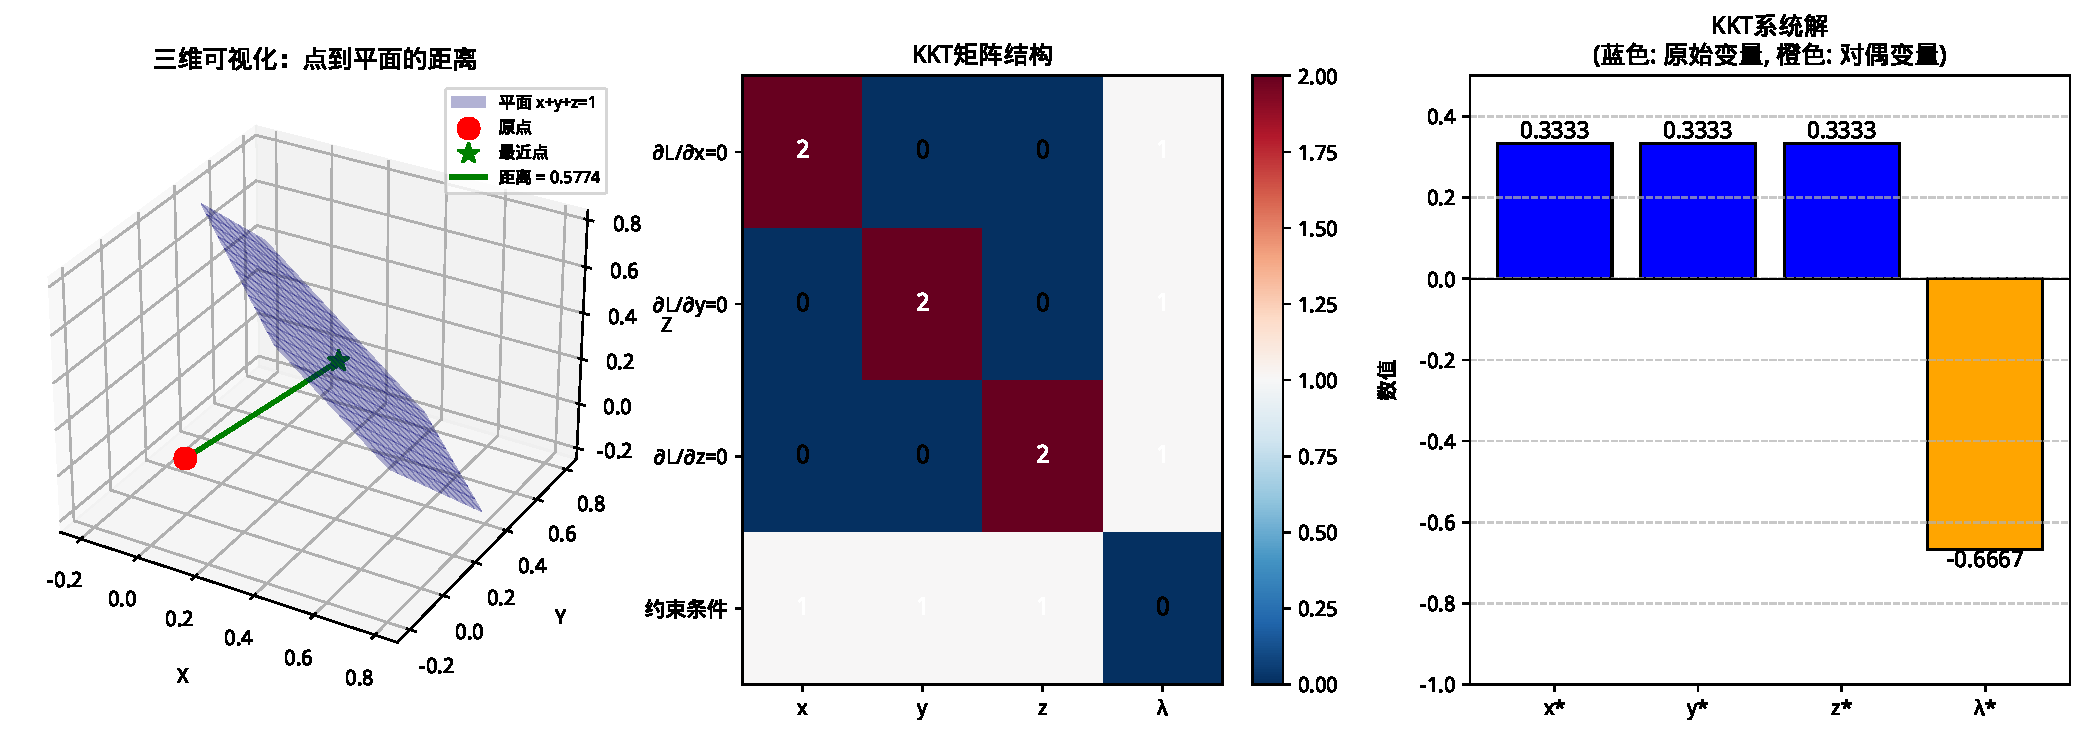
\includegraphics[width=0.85\textwidth]{figs_chap01/kkt_visualization.pdf}
\caption{KKT系统的可视化（1行3列）。\textbf{左图}：3D几何——蓝色平面为约束$x+y+z=1$，红点为原点，绿色星号为最近点，连线表示最短距离；\textbf{中图}：KKT矩阵结构热力图——矩阵有鞍点结构，对角块来自目标函数Hessian（$2I$），非对角块来自约束梯度；\textbf{右图}：KKT系统的解——蓝色柱子为原始变量$(x^*,y^*,z^*)=(1/3,1/3,1/3)$，橙色柱子为拉格朗日乘子$\lambda^*=-2/3$（负号表示约束放松会减小目标值）。}
\label{fig:chap01_kkt}
\end{figure}

\begin{figure}[htbp]
\centering
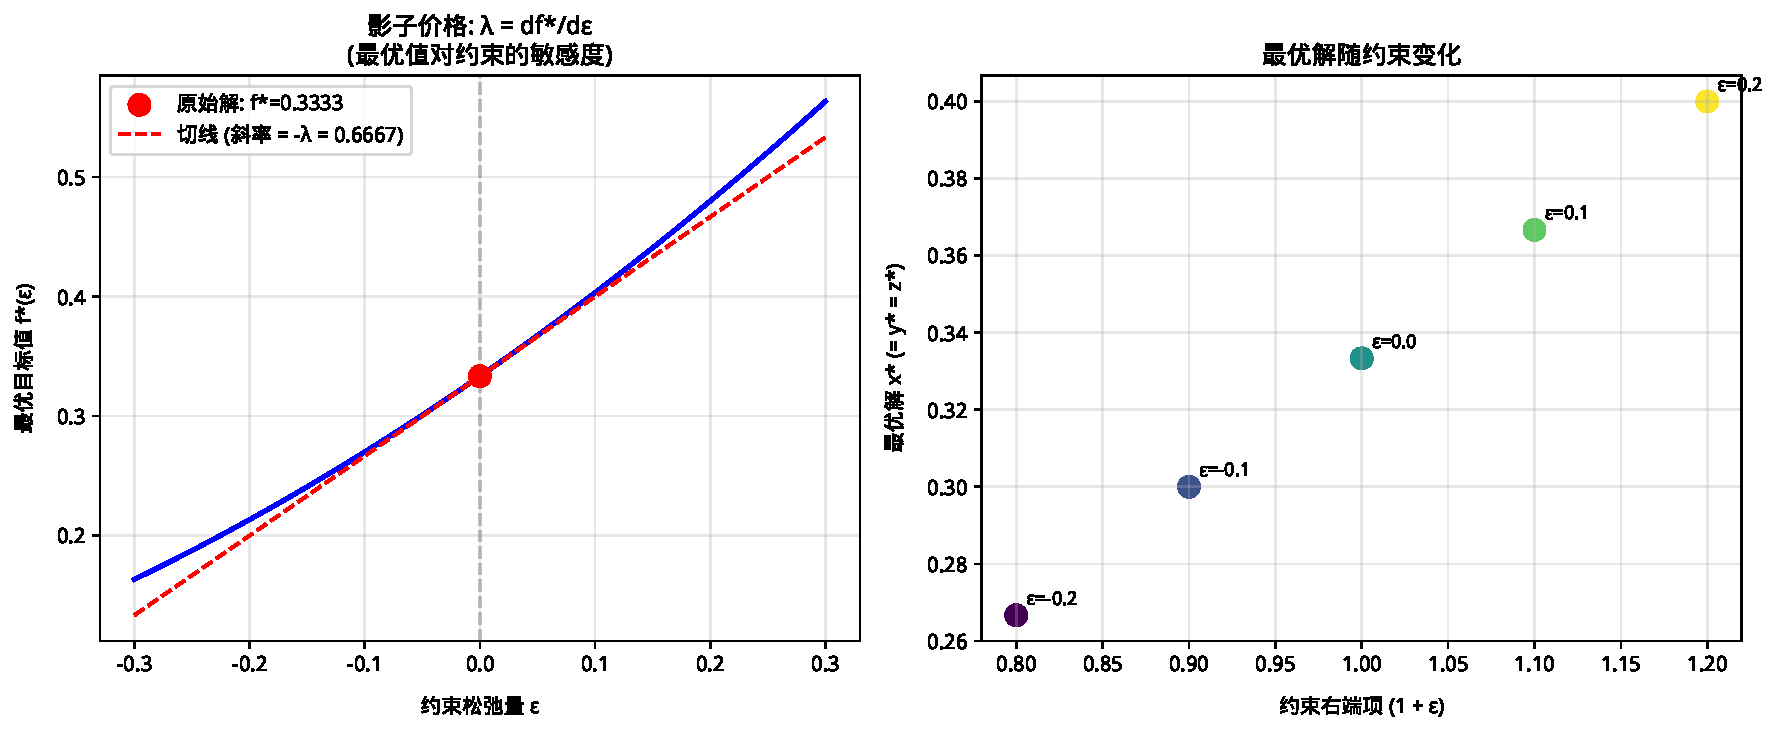
\includegraphics[width=0.85\textwidth]{figs_chap01/shadow_price.pdf}
\caption{牛顿法求解非线性约束优化的收敛过程。通过迭代求解KKT系统，算法从初始点快速收敛到约束曲面上的最优解，展示了二次收敛的特性。}
\label{fig:chap01_newton}
\end{figure}

\textbf{代码验证}：使用Python求解开篇例子的KKT系统，得到$(x^*, y^*, z^*, \lambda^*) = (1/3, 1/3, 1/3, -2/3)$，与手算结果完全一致。

% ------------------------------------------------------------------------------------
\section{本章小结}

本章我们从三个视角理解了拉格朗日乘子法：

\begin{enumerate}
    \item \textbf{代数视角}：引入乘子$\lambda$，让"变量数 = 方程数"，把约束优化变成解方程组

    \item \textbf{经济视角}：$\lambda$是约束的"影子价格"——放松约束能带来多少收益

    \item \textbf{罚函数视角}：约束可以"软化"为罚项，$\rho \to \infty$时趋向硬约束
\end{enumerate}

\begin{physicalmeaning}
本章的核心信息：$\lambda$是约束的\textbf{影子价格}——它告诉我们放松约束能带来多少收益。这个概念会贯穿全书：
\begin{itemize}
    \item 第4章：$\lambda$ = 约束力（杆的张力、支持力）
    \item 第7章：$\lambda$ = 接触力
    \item 第8章：$\lambda(t)$ = 协态变量（未来代价对当前状态的敏感度）
    \item 第9章：$\lambda$ = 反向传播中的误差信号
    \item 第10章：$\lambda$ = 值函数 $V(s)$
\end{itemize}
\end{physicalmeaning}


\section*{扩展阅读：二阶条件与正定性}
\addcontentsline{toc}{section}{扩展阅读：二阶条件与正定性}

驻点条件只告诉我们"候选点"，但无法区分极小、极大和鞍点。这就像知道山路的坡度为零，但不知道是在山顶、山谷、还是马鞍形的山口。

\subsubsection{先回顾：一维情况}

在一维微积分中，判断极值很简单：
\begin{itemize}
    \item $f''(x^*) > 0$ $\Rightarrow$ 极小（曲线向上弯）
    \item $f''(x^*) < 0$ $\Rightarrow$ 极大（曲线向下弯）
    \item $f''(x^*) = 0$ $\Rightarrow$ 需要更高阶信息
\end{itemize}

二阶导数的符号告诉我们：在驻点附近，函数是"碗形"还是"倒碗形"。

\subsubsection{多维情况：Hessian矩阵}

当$x \in \R^n$时，二阶导数变成了一个$n \times n$的矩阵——\textbf{Hessian矩阵}：
\[
\nabla^2 f = \begin{pmatrix}
\frac{\partial^2 f}{\partial x_1^2} & \frac{\partial^2 f}{\partial x_1 \partial x_2} & \cdots \\
\frac{\partial^2 f}{\partial x_2 \partial x_1} & \frac{\partial^2 f}{\partial x_2^2} & \cdots \\
\vdots & \vdots & \ddots
\end{pmatrix}
\]

问题来了：一维的"正"或"负"，在多维该怎么推广？

\subsubsection{正定与负定：多维的"碗形"与"倒碗形"}

关键思想是看\textbf{沿任意方向走，函数怎么变化}。

在驻点$x^*$附近，沿方向$v$走一小步$\epsilon$，函数值的变化（用泰勒展开）是：
\[
f(x^* + \epsilon v) - f(x^*) \approx \underbrace{\epsilon \nabla f \cdot v}_{=0,\text{因为是驻点}} + \frac{\epsilon^2}{2} v^T H v
\]

所以二阶变化完全由$v^T H v$决定！

\begin{center}
\fbox{\parbox{0.9\textwidth}{
\textbf{正定}：对所有非零方向$v$，都有$v^T H v > 0$

\textbf{含义}：不管往哪个方向走，函数值都会\textbf{增加}——这是一个"碗底"。
}}
\end{center}

\begin{center}
\fbox{\parbox{0.9\textwidth}{
\textbf{负定}：对所有非零方向$v$，都有$v^T H v < 0$

\textbf{含义}：不管往哪个方向走，函数值都会\textbf{减少}——这是一个"山顶"。
}}
\end{center}

\begin{center}
\fbox{\parbox{0.9\textwidth}{
\textbf{不定}：有些方向$v^T H v > 0$，有些方向$v^T H v < 0$

\textbf{含义}：某些方向上升，某些方向下降——这是一个"马鞍"。
}}
\end{center}

\textbf{具体例子}：考虑二维函数在原点的Hessian。

\begin{enumerate}
    \item $f(x,y) = x^2 + y^2$（碗形）
    \[
    H = \begin{pmatrix} 2 & 0 \\ 0 & 2 \end{pmatrix}, \quad v^T H v = 2v_1^2 + 2v_2^2 > 0 \quad \text{（正定）}
    \]

    \item $f(x,y) = -x^2 - y^2$（倒碗形）
    \[
    H = \begin{pmatrix} -2 & 0 \\ 0 & -2 \end{pmatrix}, \quad v^T H v = -2v_1^2 - 2v_2^2 < 0 \quad \text{（负定）}
    \]

    \item $f(x,y) = x^2 - y^2$（马鞍形）
    \[
    H = \begin{pmatrix} 2 & 0 \\ 0 & -2 \end{pmatrix}, \quad v^T H v = 2v_1^2 - 2v_2^2 \quad \text{（不定）}
    \]
    沿$x$方向（$v=(1,0)$）上升，沿$y$方向（$v=(0,1)$）下降。
\end{enumerate}

\subsubsection{如何判断正定性？}

实际操作中，不需要检验所有方向。有几个等价条件：

\begin{center}
\begin{tabular}{c|c}
\toprule
\textbf{判定方法} & \textbf{正定的条件} \\
\midrule
特征值 & 所有特征值 $> 0$ \\
顺序主子式 & 所有顺序主子式 $> 0$（Sylvester准则） \\
Cholesky分解 & 能成功分解为$H = LL^T$（$L$是下三角） \\
\bottomrule
\end{tabular}
\end{center}

\clarify{对于负定，只需检验$-H$是否正定。对于半正定（$v^T H v \geq 0$），特征值可以包含零。}

\subsubsection{约束优化的二阶条件}

现在回到约束优化。难点在于：我们只能在\textbf{约束曲面上}移动，不是整个空间。

定义\textbf{约束Hessian}（拉格朗日函数对$x$的二阶导）：
\[
H = \nabla^2_{xx} \Lag = \nabla^2 f + \sum_i \lambda_i \nabla^2 g_i
\]

\textbf{关键区别}：不需要$H$在整个空间上正定，只需要在\textbf{切空间}上正定！

切空间是什么？就是沿着约束曲面能走的方向，即满足$\nabla g_i \cdot v = 0$的所有$v$。

\begin{physicalmeaning}
\textbf{约束优化的二阶充分条件}：

设$x^*$是满足一阶条件（KKT条件）的点。如果对所有满足$\nabla g_i(x^*) \cdot v = 0$的非零方向$v$，都有
\[
v^T H v > 0
\]
则$x^*$是严格局部极小点。
\end{physicalmeaning}

\textbf{直观理解}：我们只关心"能走的方向"。即使某些方向上$H$是负的，只要那些方向被约束禁止了，就不影响极小性。

\textbf{例子}：考虑$\min x^2 - y^2$ s.t. $y = 0$。

无约束时，原点是鞍点（$H$不定）。但加上约束$y=0$后，切空间只有$x$方向，而沿$x$方向$H$是正的！所以在约束下，原点是极小点。



\subsection{矩阵形式（进阶）}

驻点条件可以写成紧凑的矩阵形式：
\[
\begin{pmatrix} \nabla f \\ g \end{pmatrix} + \begin{pmatrix} (\nabla g)^T \\ 0 \end{pmatrix} \lambda = 0
\]

或者更对称地，定义增广系统：
\[
\begin{pmatrix} \nabla^2_{xx}\Lag & (\nabla g)^T \\ \nabla g & 0 \end{pmatrix} \begin{pmatrix} \Delta x \\ \lambda \end{pmatrix} = -\begin{pmatrix} \nabla_x \Lag \\ g \end{pmatrix}
\]

这正是牛顿法求解约束优化的核心迭代格式（KKT系统）。左边的大矩阵叫做\textbf{KKT矩阵}。

\preview{这个矩阵结构会在第7章（机器人动力学）以"质量矩阵+约束雅可比"的形式再次出现。}

% ------------------------------------------------------------------------------------
\section{习题}

\paragraph{计算题}

\begin{enumerate}
    \item 对于约束$g_1(x,y,z) = x^2 + y^2 + z^2 - 1$（单位球面）和$g_2(x,y,z) = x + y - z$（平面），写出雅可比矩阵$\nabla g$，并验证它是$2 \times 3$的矩阵。
    
    \item 考虑问题$\min (x-1)^2 + (y-1)^2$ s.t. $x + y = 1$。
    \begin{enumerate}
        \item 写出拉格朗日函数$\Lag(x, y, \lambda)$
        \item 写出KKT矩阵，并验证它是$3 \times 3$的
        \item 直接求解KKT系统，得到$(x^*, y^*, \lambda^*)$
    \end{enumerate}
    
    \item 对于$2 \times 2$的KKT矩阵$K = \begin{pmatrix} 2 & 1 \\ 1 & 0 \end{pmatrix}$，计算其特征值，验证$K$是不定的（有正有负的特征值）。
\end{enumerate}

\paragraph{编程题}

\begin{enumerate}
    \setcounter{enumi}{3}
    \item 用Python/NumPy直接求解开篇例子的KKT系统：
    \[
    \begin{pmatrix} 
    2 & 0 & 0 & 1 \\
    0 & 2 & 0 & 1 \\
    0 & 0 & 2 & 1 \\
    1 & 1 & 1 & 0
    \end{pmatrix}
    \begin{pmatrix} x \\ y \\ z \\ \lambda \end{pmatrix} = 
    \begin{pmatrix} 0 \\ 0 \\ 0 \\ 1 \end{pmatrix}
    \]
    用\texttt{numpy.linalg.solve}求解，并与手算结果$(1/3, 1/3, 1/3, -2/3)$对比。
    
    \item 实现牛顿法求解非线性约束问题$\min x^2 + y^2$ s.t. $x^2 + xy + y^2 = 1$：
    \begin{enumerate}
        \item 写出KKT方程组（残差$r$）
        \item 写出KKT矩阵（残差对$(x,y,\lambda)$的雅可比）
        \item 从初始点$(1, 0, 0)$开始迭代，观察收敛过程
    \end{enumerate}
    
    \item 做实验：生成随机的正定矩阵$H$和随机的约束雅可比$A$，构造KKT矩阵$K = \begin{pmatrix} H & A^T \\ A & 0 \end{pmatrix}$。计算$K$的特征值，验证：（a）$K$总是不定的；（b）正特征值的个数等于$H$的维度，负特征值的个数等于$A$的行数。
\end{enumerate}

\paragraph{思考题}

\begin{enumerate}
    \setcounter{enumi}{6}
    \item KKT矩阵的右下角为什么是零块？如果约束函数$g$依赖于$\lambda$，会发生什么？（提示：约束的物理意义）
    
    \item 当约束数$m$远小于变量数$n$时，为什么用Schur补方法（先解$m \times m$的小系统）比直接解$(n+m) \times (n+m)$的大系统更高效？估算两种方法的计算复杂度。
    
    \item 在机器人动力学中，KKT矩阵以"质量矩阵+约束雅可比"的形式出现。猜测：$H$对应什么物理量？$\nabla g$对应什么？$\lambda$的物理意义是什么？（提示：第7章会详细讨论）
\end{enumerate}

% ------------------------------------------------------------------------------------
\section*{扩展阅读：什么是凸优化？}
\addcontentsline{toc}{section}{扩展阅读：凸优化}

在本章我们学习了约束优化的一般理论。但有一类特殊的优化问题——\textbf{凸优化}——具有非常好的性质，在机器学习和工程中应用极其广泛。

\subsection*{凸集与凸函数}

\begin{definition}[凸集]
一个集合$\mathcal{C}$是\textbf{凸集}，如果对于$\mathcal{C}$中任意两点$x, y$，连接它们的线段也完全在$\mathcal{C}$内：
\[
\forall x, y \in \mathcal{C}, \forall \theta \in [0,1]: \quad \theta x + (1-\theta)y \in \mathcal{C}
\]
\end{definition}

\begin{figure}[htbp]
\centering
\begin{tikzpicture}[scale=0.8]
    % 凸集
    \begin{scope}[shift={(0,0)}]
        \draw[thick, fill=blue!15] (0,0) ellipse (1.5cm and 1cm);
        \fill (0.5,0.3) circle (2pt) node[above] {$x$};
        \fill (-0.7,-0.2) circle (2pt) node[below] {$y$};
        \draw[red, thick] (0.5,0.3) -- (-0.7,-0.2);
        \node at (0,-1.5) {凸集 $\checkmark$};
    \end{scope}

    % 非凸集
    \begin{scope}[shift={(5,0)}]
        \draw[thick, fill=red!15] plot[smooth cycle] coordinates {(0,1) (1.2,0.5) (1,-0.5) (0.3,-0.8) (-0.5,-0.3) (-1,0.3) (-0.3,0.8)};
        \fill (0.8,0.3) circle (2pt) node[above] {$x$};
        \fill (-0.6,0.2) circle (2pt) node[above] {$y$};
        \draw[red, thick, dashed] (0.8,0.3) -- (-0.6,0.2);
        \node at (0,-1.5) {非凸集 $\times$};
    \end{scope}
\end{tikzpicture}
\caption{凸集的直观理解：线段不会``跑出去''}
\end{figure}

\begin{definition}[凸函数]
函数$f: \R^n \to \R$是\textbf{凸函数}，如果它的图形``向下弯曲''：
\[
f(\theta x + (1-\theta)y) \leq \theta f(x) + (1-\theta)f(y), \quad \forall \theta \in [0,1]
\]
等价地，$f$是凸函数当且仅当它的Hessian矩阵半正定：$\nabla^2 f \succeq 0$。
\end{definition}

\textbf{直观理解}：凸函数的图像像一个``碗''——任意两点之间的弦总在曲线上方。

\begin{example}[常见凸函数]
\begin{itemize}
    \item \textbf{线性函数}：$f(x) = a^T x + b$（既是凸函数也是凹函数）
    \item \textbf{二次函数}：$f(x) = \frac{1}{2}x^T Q x + b^T x$，当$Q \succeq 0$时是凸函数
    \item \textbf{范数}：$f(x) = \|x\|_p$（任何$p \geq 1$）
    \item \textbf{指数函数}：$f(x) = e^x$
    \item \textbf{负对数}：$f(x) = -\log x$（$x > 0$）
    \item \textbf{交叉熵损失}：深度学习中常用的损失函数
\end{itemize}
\end{example}

\subsection*{凸优化问题的定义}

\begin{definition}[凸优化问题]
一个优化问题是\textbf{凸优化问题}，如果：
\begin{enumerate}
    \item 目标函数$f(x)$是凸函数
    \item 不等式约束$g_i(x) \leq 0$中，每个$g_i$都是凸函数
    \item 等式约束$h_j(x) = 0$中，每个$h_j$都是仿射函数（线性函数）
\end{enumerate}
\end{definition}

\subsection*{凸优化的``好''性质}

凸优化问题有一个极其重要的性质，使它在实践中非常有用：

\begin{keytheorem}[title=凸优化的核心定理]
对于凸优化问题：
\begin{enumerate}
    \item \textbf{局部最优 = 全局最优}：任何局部最小点都是全局最小点
    \item \textbf{KKT条件是充分条件}：满足KKT条件的点一定是全局最优解（不只是候选点）
    \item \textbf{高效算法}：存在多项式时间算法求解（如内点法）
\end{enumerate}
\end{keytheorem}

\begin{physicalmeaning}
为什么``局部=全局''如此重要？

想象你在山里找最低点。对于一般的地形（非凸），你可能陷入一个山谷（局部最小），却不知道旁边还有更深的山谷。

但如果地形是凸的（只有一个``碗底''），那么你只要一直往下走，最终一定能到达最低点。\textbf{不需要担心被骗到假的最低点！}

这就是为什么机器学习中很多人喜欢用凸损失函数——优化更简单，更可靠。
\end{physicalmeaning}

\subsection*{为什么深度学习是非凸的？}

你可能会问：既然凸优化这么好，为什么深度学习不用凸优化？

答案是：\textbf{神经网络的损失函数天然是非凸的}。

\begin{example}[非凸性的来源]
考虑一个简单的两层神经网络：$f(x; w_1, w_2) = w_2 \cdot \sigma(w_1 \cdot x)$

即使激活函数$\sigma$是凸的，复合之后损失函数关于参数$(w_1, w_2)$也不是凸的。

直观原因：如果我们交换$w_1$和$-w_1$，同时翻转$w_2$的符号，网络输出可能不变——这意味着参数空间有很多``等效''的点，形成复杂的非凸景观。
\end{example}

\textbf{好消息是}：虽然深度学习是非凸的，但实践表明：
\begin{itemize}
    \item 大多数局部最小点的性能都差不多好
    \item 鞍点（而非局部最小点）才是主要障碍
    \item SGD等算法能有效逃离鞍点
\end{itemize}

\subsection*{凸优化在机器学习中的应用}

虽然深度学习是非凸的，但很多经典机器学习问题是凸优化问题：

\begin{center}
\renewcommand{\arraystretch}{1.3}
\begin{tabular}{l|l|l}
\toprule
\textbf{问题} & \textbf{目标函数} & \textbf{是否凸？} \\
\midrule
线性回归 & $\|Ax - b\|^2$ & 凸 \\
岭回归 & $\|Ax - b\|^2 + \lambda\|x\|^2$ & 凸 \\
LASSO & $\|Ax - b\|^2 + \lambda\|x\|_1$ & 凸 \\
支持向量机(SVM) & $\frac{1}{2}\|w\|^2 + C\sum_i \xi_i$ & 凸 \\
逻辑回归 & $\sum_i \log(1 + e^{-y_i w^T x_i})$ & 凸 \\
\midrule
神经网络 & 交叉熵/MSE关于参数 & \textbf{非凸} \\
\bottomrule
\end{tabular}
\end{center}

\begin{insightbox}
\textbf{实用建议}：
\begin{itemize}
    \item 如果你的问题可以建模为凸优化，\textbf{优先用凸优化}——解是全局最优的，算法可靠
    \item 如果必须用非凸模型（如深度学习），\textbf{多试几个初始点}，或用预训练模型
    \item 学习\texttt{cvxpy}库——Python中最好用的凸优化工具
\end{itemize}
\end{insightbox}  % 第1章：从高数到约束优化
% ====================================================================================
\chapter{对偶理论：换个角度看问题}
% ====================================================================================

\section*{一个迟到的研究生}

\marginnote{\textbf{乔治·丹齐格}(1914--2005)：线性规划之父，单纯形法发明人。他``误把未解决问题当作业解决''的故事成为传奇，启发了电影《心灵捕手》。1975年获美国国家科学奖章，被誉为``20世纪最重要的应用数学家之一''。}

1939年秋天的一个清晨，加州大学伯克利分校的研究生George Dantzig迟到了。当他匆忙走进统计学课堂时，Jerzy Neyman教授正在黑板上写着两道题目。Dantzig以为那是这周的作业，就把题目抄下来了。

接下来的几天，Dantzig发现这两道"作业"异常困难。但他没有放弃，花了好几个晚上反复尝试。几天后，他把解答交给教授，有些尴尬地说："这作业有点难，我花了不少时间。能不能宽限一下？"

Neyman教授看着解答，沉默了很久。然后他说出了一句让Dantzig震惊的话：

"这不是作业。这是我在课上提到的两个\textbf{著名的未解决问题}，用来说明统计学前沿有多困难。你……把它们都解决了。"

\clarify{这个故事后来成为电影《心灵捕手》的灵感来源。Dantzig因为不知道问题是"不可能的"，所以没有心理障碍，反而解决了它们。}

\section*{从战争中诞生的对偶理论}

1947年，第二次世界大战刚刚结束。美国空军面临一个巨大的后勤难题：如何以最低成本调度数千架飞机、协调数百个基地的物资供应？

Dantzig被指派解决这个问题。他首先将问题形式化为\textbf{线性规划}（Linear Programming），然后发现了一个惊人的事实：

\begin{center}
\fbox{\parbox{0.9\textwidth}{
每一个优化问题都有一个"镜像"版本。原问题问的是"用多少资源"，镜像问题问的是"资源值多少钱"。

神奇的是：这两个问题的最优值\textbf{相等}！更妙的是：有时候镜像问题比原问题\textbf{更容易求解}。
}}
\end{center}

这就是\textbf{对偶理论}的起源。它不是纯数学的抽象游戏，而是从实际的军事后勤问题中诞生的。

\vspace{0.5cm}
\noindent\textit{想象你是一个快递公司的调度员，需要优化100辆货车的路线。直接求解需要考虑$100!$种可能——这个数字比宇宙中的原子数还多。但如果换个角度，从"每条路的使用成本"来思考，问题可能突然变得简单了。}

\begin{quote}
\textbf{本章目标}：理解为什么有时候"绕个弯"反而更快——对偶问题可能比原问题更容易求解。这不仅是计算技巧，更是拉格朗日乘子法的自然延伸。
\end{quote}

\begin{tcolorbox}[colback=green!5, colframe=green!60!black, title=学完这章，你将能够...]
\begin{itemize}
    \item 写出任意优化问题的对偶问题
    \item 利用弱对偶性获得原问题的下界（用于算法验证）
    \item 判断何时强对偶成立，从而用对偶问题替代原问题求解
    \item 理解SVM、最大熵模型等机器学习算法背后的对偶结构
    \item 用互补松弛条件从对偶解恢复原问题的解
\end{itemize}
\end{tcolorbox}

% ------------------------------------------------------------------------------------
\section{从拉格朗日函数到对偶}

\subsection{回顾：拉格朗日函数}

在第1章，我们学习了拉格朗日函数：
\[
\Lag(x, \lambda) = f(x) + \lambda^\top g(x)
\]

关键洞察是：对于满足约束$g(x) = 0$的点，$\Lag$和$f$的取值完全一样。

现在我们要问一个新问题：这个函数有两个变量$x$和$\lambda$，如果要找它的"最优点"，应该怎么办？

\subsection{两种优化顺序}

拉格朗日函数$\Lag(x, \lambda)$是两组变量的函数。一个自然的问题是：我们应该先优化$x$还是先优化$\lambda$？

答案是：\textbf{先优化谁，结果可能不一样！}

\textbf{顺序A}：先固定$\lambda$，对$x$求最小值；然后再对$\lambda$求最大值
\[
\max_\lambda \min_x \Lag(x, \lambda)
\]

\textbf{顺序B}：先固定$x$，对$\lambda$求最大值；然后再对$x$求最小值
\[
\min_x \max_\lambda \Lag(x, \lambda)
\]

\textbf{关键问题}：这两种顺序得到的结果一样吗？

让我们通过两个例子来看。

\subsubsection{例1：矩阵博弈}

考虑一个资源分配问题。行玩家（攻方）选择进攻方向$i \in \{1,2,3,4\}$，列玩家（守方）选择防守位置$j \in \{1,2,3,4\}$。矩阵元素$a_{ij}$表示攻方的损失：

\[
A = \begin{pmatrix}
7 & 2 & 5 & 9 \\
3 & 6 & 8 & 4 \\
5 & 4 & 3 & 7 \\
6 & 8 & 4 & 2
\end{pmatrix}
\]

攻方想让损失\textbf{最小}，守方想让攻方损失\textbf{最大}。

\vspace{0.3cm}
\textbf{顺序A}：$\max_j \min_i a_{ij}$（守方先选，攻方后选）

\begin{center}
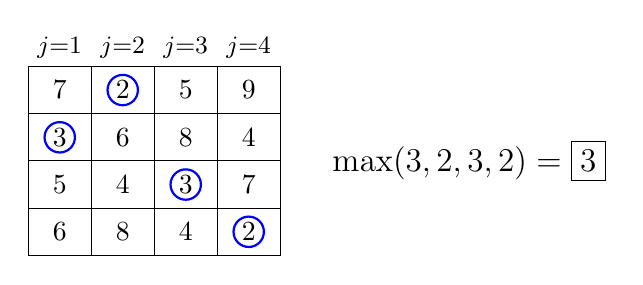
\begin{tikzpicture}[scale=0.8]
    % 矩阵框架
    \draw (0, 0) rectangle (4, 3);
    \draw (1, 0) -- (1, 3); \draw (2, 0) -- (2, 3); \draw (3, 0) -- (3, 3);
    \draw (0, 0.75) -- (4, 0.75); \draw (0, 1.5) -- (4, 1.5); \draw (0, 2.25) -- (4, 2.25);
    
    % 列标签
    \node[font=\small] at (0.5, 3.3) {$j$=1}; \node[font=\small] at (1.5, 3.3) {$j$=2}; 
    \node[font=\small] at (2.5, 3.3) {$j$=3}; \node[font=\small] at (3.5, 3.3) {$j$=4};
    
    % 矩阵元素，高亮每列最小值
    \node at (0.5, 2.625) {7}; \node at (1.5, 2.625) {\tikz\node[circle,draw=blue,thick,inner sep=1pt]{2};}; \node at (2.5, 2.625) {5}; \node at (3.5, 2.625) {9};
    \node at (0.5, 1.875) {\tikz\node[circle,draw=blue,thick,inner sep=1pt]{3};}; \node at (1.5, 1.875) {6}; \node at (2.5, 1.875) {8}; \node at (3.5, 1.875) {4};
    \node at (0.5, 1.125) {5}; \node at (1.5, 1.125) {4}; \node at (2.5, 1.125) {\tikz\node[circle,draw=blue,thick,inner sep=1pt]{3};}; \node at (3.5, 1.125) {7};
    \node at (0.5, 0.375) {6}; \node at (1.5, 0.375) {8}; \node at (2.5, 0.375) {4}; \node at (3.5, 0.375) {\tikz\node[circle,draw=blue,thick,inner sep=1pt]{2};};
    

    % 箭头和最终结果
    \node[font=\large\bfseries] at (7, 1.5) {$\max(3,2,3,2) = \boxed{3}$};
\end{tikzpicture}
\end{center}

\textbf{顺序B}：$\min_i \max_j a_{ij}$（攻方先选，守方后选）

\begin{center}
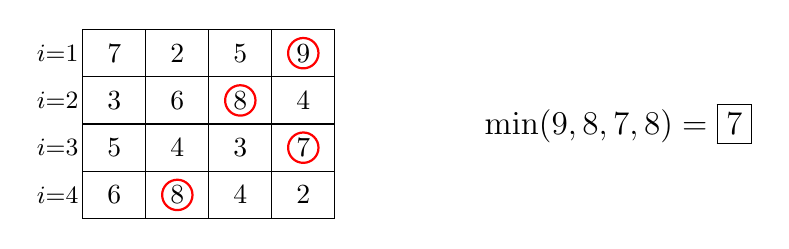
\begin{tikzpicture}[scale=0.8]
    % 矩阵框架
    \draw (0, 0) rectangle (4, 3);
    \draw (1, 0) -- (1, 3); \draw (2, 0) -- (2, 3); \draw (3, 0) -- (3, 3);
    \draw (0, 0.75) -- (4, 0.75); \draw (0, 1.5) -- (4, 1.5); \draw (0, 2.25) -- (4, 2.25);
    
    % 行标签
    \node[font=\small] at (-0.4, 2.625) {$i$=1}; \node[font=\small] at (-0.4, 1.875) {$i$=2}; 
    \node[font=\small] at (-0.4, 1.125) {$i$=3}; \node[font=\small] at (-0.4, 0.375) {$i$=4};
    
    % 矩阵元素，高亮每行最大值
    \node at (0.5, 2.625) {7}; \node at (1.5, 2.625) {2}; \node at (2.5, 2.625) {5}; \node at (3.5, 2.625) {\tikz\node[circle,draw=red,thick,inner sep=1pt]{9};};
    \node at (0.5, 1.875) {3}; \node at (1.5, 1.875) {6}; \node at (2.5, 1.875) {\tikz\node[circle,draw=red,thick,inner sep=1pt]{8};}; \node at (3.5, 1.875) {4};
    \node at (0.5, 1.125) {5}; \node at (1.5, 1.125) {4}; \node at (2.5, 1.125) {3}; \node at (3.5, 1.125) {\tikz\node[circle,draw=red,thick,inner sep=1pt]{7};};
    \node at (0.5, 0.375) {6}; \node at (1.5, 0.375) {\tikz\node[circle,draw=red,thick,inner sep=1pt]{8};}; \node at (2.5, 0.375) {4}; \node at (3.5, 0.375) {2};
    

    % 箭头和最终结果
    \node[font=\large\bfseries] at (8.5, 1.5) {$\min(9,8,7,8) = \boxed{7}$};
\end{tikzpicture}
\end{center}

\vspace{0.2cm}
\begin{center}
\fbox{\parbox{0.85\textwidth}{
\textbf{结论}：$\displaystyle\max_j \min_i = 3 \neq 7 = \min_i \max_j$

两种顺序差了4！后行动的玩家能看到对方的选择再做决策，天然占优势。
}}
\end{center}


\subsubsection{例2：连续函数}

考虑函数
\[
F(x, y) = -x^2 + xy, \quad x \in \R, \; y \in [-2, 2]
\]

\textbf{顺序A}：$\displaystyle\max_{y \in [-2,2]} \min_{x \in \R} (-x^2 + xy)$

\begin{center}
\begin{tikzpicture}[scale=0.8]
    % Step 1: 固定y，对x求min
    \node[blue, font=\bfseries] at (0, 3) {Step 1: 固定$y$，对$x$求$\min$};
    
    \node at (0, 2.2) {$\displaystyle\pd{F}{x} = -2x + y = 0 \;\Rightarrow\; x^* = \frac{y}{2}$};
    
    \node at (0, 1.2) {代入：$\displaystyle F\Big(\frac{y}{2}, y\Big) = -\frac{y^2}{4} + \frac{y^2}{2} = \frac{y^2}{4}$};
    
    % Step 2
    \node[red, font=\bfseries] at (0, 0) {Step 2: 对$y$求$\max$};
    
    \node at (0, -0.9) {$\displaystyle\max_{y \in [-2,2]} \frac{y^2}{4} = \frac{4}{4} = 1$（在$y = \pm 2$）};
    
    \draw[thick, ->] (4, 1) -- (5.5, 1);
    \node[font=\Large\bfseries, red] at (7, 1) {结果 $= 1$};
\end{tikzpicture}
\end{center}

\textbf{顺序B}：$\displaystyle\min_{x \in \R} \max_{y \in [-2,2]} (-x^2 + xy)$

\begin{center}
\begin{tikzpicture}[scale=0.8]
    % Step 1: 固定x，对y求max
    \node[blue, font=\bfseries] at (0, 3) {Step 1: 固定$x$，对$y$求$\max$};
    
    \node at (0, 2.1) {$F = -x^2 + xy$ 关于$y$是线性的};
    
    \node at (0, 0.5) {$\begin{cases} x > 0: & \max\text{在 } y=2, \; F = -x^2 + 2x \\ x < 0: & \max\text{在 } y=-2, \; F = -x^2 - 2x \\ x = 0: & F = 0 \end{cases}$};
    
    % Step 2
    \node[red, font=\bfseries] at (0, -1.3) {Step 2: 对$x$求$\min$};
    
    \node at (0, -2.2) {$\displaystyle\max_y F = -x^2 + 2|x| = -(|x|-1)^2 + 1$};
    
    \node at (0, -3.5) {这是开口向下的抛物线，最大值$1$在$|x|=1$，最小值$0$在$x=0$};
    
    \draw[thick, ->] (4.5, -4) -- (6, -4);
    \node[font=\Large\bfseries, red] at (7.5, -4) {结果 $= 0$};
\end{tikzpicture}
\end{center}

% 画函数图
\begin{figure}[h]
\centering
\begin{tikzpicture}[scale=0.9]
    % 左图：顺序A
    \begin{scope}[xshift=0cm]
        \draw[->] (-2.5, 0) -- (2.5, 0) node[right] {$y$};
        \draw[->] (0, -0.5) -- (0, 1.5) node[above] {$g(y)$};
        \draw[thick, blue, domain=-2:2, samples=50] plot (\x, {\x*\x/4});
        \fill[red] (-2, 1) circle (2pt);
        \fill[red] (2, 1) circle (2pt);
        \node[below] at (0, -0.8) {$g(y) = y^2/4$};
        \node[red, right] at (2.1, 1) {\small $\max = 1$};
        \node[below] at (0, -1.5) {\textbf{顺序A}：$\max_y g(y) = 1$};
    \end{scope}
    
    % 右图：顺序B
    \begin{scope}[xshift=7cm]
        \draw[->] (-2.5, 0) -- (2.5, 0) node[right] {$x$};
        \draw[->] (0, -0.5) -- (0, 1.5) node[above] {$h(x)$};
        \draw[thick, blue, domain=-2:0, samples=50] plot (\x, {-\x*\x - 2*\x});
        \draw[thick, blue, domain=0:2, samples=50] plot (\x, {-\x*\x + 2*\x});
        \fill[red] (0, 0) circle (2pt);
        \fill[blue] (-1, 1) circle (2pt);
        \fill[blue] (1, 1) circle (2pt);
        \node[below] at (0, -0.8) {$h(x) = -x^2 + 2|x|$};
        \node[red, right] at (0.1, -0.2) {\small $\min = 0$};
        \node[below] at (0, -1.5) {\textbf{顺序B}：$\min_x h(x) = 0$};
    \end{scope}
\end{tikzpicture}
\caption{两种优化顺序得到不同的中间函数，最终结果也不同}
\end{figure}

\begin{center}
\fbox{\parbox{0.85\textwidth}{
\textbf{结论}：$\displaystyle\max_y \min_x F = 1 \neq 0 = \min_x \max_y F$

同样的函数，不同的优化顺序，差了1！
}}
\end{center}

\subsubsection{规律总结}

\begin{center}
\begin{tikzpicture}
    \draw[thick, rounded corners, fill=blue!10] (0, 0) rectangle (6.5, 2.5);
    \node[font=\bfseries] at (3.25, 2) {Max-Min 不等式};
    \node at (3.25, 1.2) {$\displaystyle\max_y \min_x F(x,y) \;\leq\; \min_x \max_y F(x,y)$};
    \node[font=\small] at (3.25, 0.4) {后行动者占优势，结果更有利于他};
\end{tikzpicture}
\end{center}

\textbf{直观理解}：后行动的玩家能\textbf{看到对方的选择再决策}，所以总是占优势。

\begin{itemize}
    \item 顺序A中，$y$先选，$x$后选——$x$占优势，能把结果压低
    \item 顺序B中，$x$先选，$y$后选——$y$占优势，能把结果抬高
    \item 所以顺序A的结果 $\leq$ 顺序B的结果
\end{itemize}

\begin{insightbox}
\textbf{对偶间隙}：把这个不等式应用到拉格朗日函数：
\[
\underbrace{\max_\lambda \min_x \Lag(x, \lambda)}_{\text{对偶问题最优值}} \;\leq\; \underbrace{\min_x \max_\lambda \Lag(x, \lambda)}_{\text{原问题最优值}}
\]
左右两边的差叫做\textbf{对偶间隙}（duality gap）。

对于\textbf{凸优化}问题，在适当条件下（Slater条件），对偶间隙为零——这就是\textbf{强对偶性}，意味着两种顺序给出相同结果。
\end{insightbox}



\section{博弈论视角：对偶的直觉来源}

\subsection{一个思想实验}

在深入数学推导之前，让我们先用一个博弈的比喻来理解对偶的本质。

想象 $x$ 和 $\lambda$ 是两个玩家在玩一个\textbf{零和博弈}。他们面对同一个函数——拉格朗日函数 $\mathcal{L}(x, \lambda)$，但目标相反：

\begin{itemize}
    \item \textbf{玩家 $x$}：想让 $\mathcal{L}$ 尽量\textbf{小}（他是"最小化者"）
    \item \textbf{玩家 $\lambda$}：想让 $\mathcal{L}$ 尽量\textbf{大}（他是"最大化者"）
\end{itemize}

现在问一个关键问题：\textbf{谁先出牌？}

\subsection{先手劣势}

在大多数博弈中，先出牌的人会吃亏——因为后手可以看到先手的选择，然后针对性地做出最优响应。

\begin{example}[石头剪刀布]
如果你先出，对方后出，你永远赢不了。对方看到你出石头，就出布；看到你出剪刀，就出石头。

先手必败，后手必胜。
\end{example}

\begin{example}[讨价还价]
买卖双方谈判。如果卖家先报价，买家可以针对这个价格压价；如果买家先出价，卖家可以针对性地抬高。

谁先开口，谁就暴露了自己的底线。
\end{example}

同样的道理适用于 $x$ 和 $\lambda$ 的博弈：

\begin{center}
\renewcommand{\arraystretch}{1.5}
\begin{tabular}{c|c|c}
\toprule
 & \textbf{$x$ 先出牌} & \textbf{$\lambda$ 先出牌} \\
\midrule
数学表达 & $\displaystyle\min_x \max_\lambda \mathcal{L}(x,\lambda)$ & $\displaystyle\max_\lambda \min_x \mathcal{L}(x,\lambda)$ \\
\midrule
谁吃亏？ & $x$ 吃亏 & $\lambda$ 吃亏 \\
\midrule
为什么？ & $\lambda$ 看到 $x$ 的选择后， & $x$ 看到 $\lambda$ 的选择后， \\
 & 可以选最大的 $\mathcal{L}$ & 可以选最小的 $\mathcal{L}$ \\
\bottomrule
\end{tabular}
\end{center}

\subsection{弱对偶定理的直觉}

既然先手吃亏，那么：

\begin{itemize}
    \item 当 $x$ 先出牌时，$\lambda$ 可以把 $\mathcal{L}$ 推高 $\Rightarrow$ 结果偏大
    \item 当 $\lambda$ 先出牌时，$x$ 可以把 $\mathcal{L}$ 压低 $\Rightarrow$ 结果偏小
\end{itemize}

所以必然有：
\[
\underbrace{\min_x \max_\lambda \mathcal{L}(x,\lambda)}_{x\text{ 先出牌，吃亏，结果大}} \;\geq\; \underbrace{\max_\lambda \min_x \mathcal{L}(x,\lambda)}_{\lambda\text{ 先出牌，吃亏，结果小}}
\]

这就是\textbf{弱对偶定理}！

\begin{keytheorem}[title=弱对偶定理]
对于任何函数 $\mathcal{L}(x, \lambda)$：
\[
\min_x \max_\lambda \mathcal{L} \;\geq\; \max_\lambda \min_x \mathcal{L}
\]

左边称为\textbf{原始问题}的最优值，右边称为\textbf{对偶问题}的最优值。

弱对偶说：原始最优值 $\geq$ 对偶最优值。
\end{keytheorem}

\subsection{强对偶：什么时候先后手无所谓？}

弱对偶告诉我们 $\min\max \geq \max\min$。但在某些"好的"问题中，两者相等！

\begin{keytheorem}[title=强对偶定理（非正式版）]
如果原始问题是\textbf{凸优化问题}，并且满足一定的正则条件（如 Slater 条件），则：
\[
\min_x \max_\lambda \mathcal{L} \;=\; \max_\lambda \min_x \mathcal{L}
\]

这意味着：无论谁先出牌，最终的博弈结果是一样的！
\end{keytheorem}

\begin{physicalmeaning}
强对偶成立时，博弈达到了\textbf{纳什均衡}——双方都没有动机单方面改变策略。

在经济学中，这对应于\textbf{市场均衡}：买家的出价恰好等于卖家能接受的最低价，双方都无法通过单方面改变获得更好的结果。
\end{physicalmeaning}

\begin{insightbox}
\textbf{弱对偶}：$\min\max \geq \max\min$，先手吃亏。这对任何问题都成立。

\textbf{强对偶}：$\min\max = \max\min$，先后手无所谓。这对"好的"凸问题成立。

强对偶是优化理论中最深刻的结果之一——它让我们可以选择更容易求解的那个问题（原始或对偶）。
\end{insightbox}

% ------------------------------------------------------------------------------------
\section{从拉格朗日函数推导对偶问题}

博弈论的直觉告诉我们对偶的"why"。现在让我们看看具体的"how"——对偶问题是怎么从拉格朗日函数一步步推导出来的。

\subsection{一个具体的线性规划问题}

考虑一个工厂的生产决策问题：

\begin{example}[家具厂的困境]
一家家具厂生产桌子和椅子。

\textbf{已知信息}：
\begin{itemize}
    \item 每张桌子利润 300 元，需要 4 小时木工、2 小时油漆
    \item 每把椅子利润 200 元，需要 2 小时木工、3 小时油漆
    \item 本周可用：木工 100 小时，油漆 90 小时
\end{itemize}

\textbf{决策}：生产多少桌子（$x_1$）和椅子（$x_2$）？
\end{example}

这是一个标准的线性规划：
\[
\max_{x_1, x_2} \quad 300 x_1 + 200 x_2
\]
\[
\text{s.t.} \quad 4x_1 + 2x_2 \leq 100 \quad \text{（木工时间）}
\]
\[
2x_1 + 3x_2 \leq 90 \quad \text{（油漆时间）}
\]
\[
x_1, x_2 \geq 0
\]

用矩阵形式写成：
\[
\max_x \; c^\top x \quad \text{s.t.} \quad Ax \leq b, \; x \geq 0
\]

其中：
\[
c = \begin{pmatrix} 300 \\ 200 \end{pmatrix}, \quad
A = \begin{pmatrix} 4 & 2 \\ 2 & 3 \end{pmatrix}, \quad
b = \begin{pmatrix} 100 \\ 90 \end{pmatrix}
\]

\subsection{构造拉格朗日函数}

对约束 $Ax \leq b$ 引入拉格朗日乘子 $y \geq 0$（不等式约束的乘子必须非负，第1章讲过）：

\[
\mathcal{L}(x, y) = c^\top x + y^\top(b - Ax)
\]

\textbf{这个函数的结构}：
\begin{itemize}
    \item $c^\top x$：原始目标（利润）
    \item $y^\top(b - Ax)$：约束的"惩罚"或"奖励"
    \begin{itemize}
        \item 如果 $Ax < b$（约束有余量），$b - Ax > 0$，这一项为正
        \item 如果 $Ax > b$（违反约束），$b - Ax < 0$，这一项为负（惩罚）
    \end{itemize}
\end{itemize}

\paragraph{关键观察：重新整理}

\begin{align}
\mathcal{L}(x, y) &= c^\top x + y^\top b - y^\top A x \\
&= y^\top b + x^\top(c - A^\top y)
\end{align}

注意第二行的形式：$\mathcal{L}$ 可以写成关于 $y$ 的项加上关于 $x$ 的项。这种\textbf{对称性}是对偶理论的核心！

\subsection{推导对偶问题}

根据博弈论视角，对偶问题是 $\max_y \min_x \mathcal{L}$。我们分两步来做：

\paragraph{第一步：固定 $y$，对 $x$ 求最小值}

看表达式 $\mathcal{L} = y^\top b + x^\top(c - A^\top y)$。

这是关于 $x$ 的线性函数。对于线性函数，最小值要么是 $-\infty$（如果系数非零），要么在边界取到。

具体来说：
\begin{itemize}
    \item 如果 $(c - A^\top y)$ 有任何正分量，比如第 $i$ 个分量 $(c - A^\top y)_i > 0$
    \item 那么令 $x_i \to -\infty$（但我们有 $x \geq 0$，所以这不行）
    \item 或者换个角度：如果我们要最大化 $\mathcal{L}$（原始问题），令 $x_i \to +\infty$ 就能让 $\mathcal{L} \to +\infty$
\end{itemize}

为了让 $\min_x \mathcal{L}$ 有界（有限值），必须要求：
\[
c - A^\top y \leq 0 \quad \Leftrightarrow \quad A^\top y \geq c
\]

在这个条件下，由于 $x \geq 0$ 且 $c - A^\top y \leq 0$，所以 $x^\top(c - A^\top y) \leq 0$。

最小值在 $x = 0$ 处取到（此时这一项等于 0）：
\[
\min_{x \geq 0} \mathcal{L}(x, y) = y^\top b \quad \text{（当 $A^\top y \geq c$ 时）}
\]

如果 $A^\top y \geq c$ 不成立，则 $\min_x \mathcal{L} = -\infty$。

\paragraph{第二步：对 $y$ 求最大值}

现在我们要：
\[
\max_{y \geq 0} \left( \min_{x \geq 0} \mathcal{L}(x, y) \right) = \max_{y \geq 0} \begin{cases} y^\top b & \text{如果 } A^\top y \geq c \\ -\infty & \text{否则} \end{cases}
\]

显然，我们只关心 $A^\top y \geq c$ 的情况。所以对偶问题是：
\[
\max_{y \geq 0} \; y^\top b \quad \text{s.t.} \quad A^\top y \geq c
\]

但我们通常把对偶问题写成最小化形式。由于 $\max f = -\min(-f)$，改写成：

\[
\min_{y \geq 0} \; b^\top y \quad \text{s.t.} \quad A^\top y \geq c
\]

这就是\textbf{对偶问题}！

\begin{keyformula}[title=线性规划的原始-对偶对]
\begin{center}
\renewcommand{\arraystretch}{1.5}
\begin{tabular}{c|c}
\textbf{原始问题} & \textbf{对偶问题} \\
\hline
$\displaystyle\max_x \; c^\top x$ & $\displaystyle\min_y \; b^\top y$ \\
s.t. $Ax \leq b$ & s.t. $A^\top y \geq c$ \\
$x \geq 0$ & $y \geq 0$ \\
\end{tabular}
\end{center}

\vspace{0.3cm}
\textbf{对称性}：
\begin{itemize}
    \item 原始的目标系数 $c$ 变成对偶的约束右端 $c$
    \item 原始的约束右端 $b$ 变成对偶的目标系数 $b$
    \item 约束矩阵从 $A$ 变成 $A^\top$（转置！）
    \item $\max$ 变成 $\min$，$\leq$ 变成 $\geq$
\end{itemize}
\end{keyformula}

\subsection{对偶的经济学解释}

对偶问题有一个非常优美的经济学解释。

\begin{example}[回到家具厂]
假设有个投资商想买断你工厂这周的全部资源（木工时间和油漆时间）。他给每小时木工出价 $y_1$ 元，每小时油漆出价 $y_2$ 元。

\textbf{投资商的目标}：花最少的钱买断所有资源。
\[
\min \; 100 y_1 + 90 y_2 = b^\top y
\]

\textbf{投资商的约束}：价格要"合理"——你必须愿意卖。

什么情况下你愿意卖？如果自己生产不如把资源卖掉划算。

\begin{itemize}
    \item 生产一张桌子需要 4 小时木工 + 2 小时油漆，能赚 300 元
    \item 如果把这些资源卖掉，能得到 $4y_1 + 2y_2$ 元
    \item 你愿意卖的条件：$4y_1 + 2y_2 \geq 300$
\end{itemize}

同理，对于椅子：$2y_1 + 3y_2 \geq 200$。

这些正是对偶约束 $A^\top y \geq c$！
\end{example}

\begin{center}
\renewcommand{\arraystretch}{1.4}
\begin{tabular}{c|c}
\toprule
\textbf{原始问题} & \textbf{对偶问题} \\
\midrule
生产者视角 & 投资商视角 \\
\midrule
决策：生产多少产品 $x$ & 决策：给资源定价 $y$ \\
\midrule
目标：最大化利润 $c^\top x$ & 目标：最小化收购成本 $b^\top y$ \\
\midrule
约束：不能超出资源 $Ax \leq b$ & 约束：价格要让生产者愿意卖 $A^\top y \geq c$ \\
\bottomrule
\end{tabular}
\end{center}

\begin{keytheorem}[title=强对偶的经济学意义]
\[
c^\top x^* = b^\top y^*
\]

\textbf{最大生产利润 = 最小资源成本}

这意味着：在均衡状态下，投资商出的价格恰好等于你自己生产能赚的钱。

\begin{itemize}
    \item 如果他出价太低，你不愿意卖，宁可自己生产
    \item 如果他出价太高，他亏了（还不如让你自己生产，他买产品）
\end{itemize}

这就是\textbf{市场均衡}的数学表达！
\end{keytheorem}

\subsection{对偶变量的含义：影子价格}

对偶变量 $y_i$ 有一个重要的经济学解释：\textbf{影子价格}（Shadow Price）。

\begin{definition}[影子价格]
$y_i^*$ 是第 $i$ 种资源的\textbf{边际价值}：如果第 $i$ 种资源增加一个单位，最大利润能增加多少？
\[
y_i^* = \frac{\partial (\text{最优利润})}{\partial b_i}
\]
\end{definition}

\begin{example}[木工时间的价值]
回到家具厂问题。假设最优解下，$y_1^* = 50$ 元/小时。

这意味着：如果木工时间从 100 小时增加到 101 小时，最大利润大约能增加 50 元。

\textbf{决策启示}：
\begin{itemize}
    \item 如果能以低于 50 元/小时的价格雇佣额外木工，就值得！
    \item 如果雇佣成本高于 50 元/小时，就不划算。
\end{itemize}
\end{example}

这就是为什么对偶变量也叫"影子价格"——它告诉你资源的\textbf{真正价值}，即使这个资源没有市场价格。

% ------------------------------------------------------------------------------------
\section{互补松弛：稀缺性决定价值}

\subsection{互补松弛条件}

在原始和对偶问题的最优解处，有一个神奇的条件成立：

\begin{keytheorem}[title=互补松弛条件]
设 $x^*$ 是原始最优解，$y^*$ 是对偶最优解，则：
\[
y_i^* \cdot (b_i - (Ax^*)_i) = 0, \quad \forall i
\]

用文字说：\textbf{对偶变量}（影子价格）和\textbf{约束松弛量}（剩余资源），两者至少有一个是零。
\end{keytheorem}

\subsection{直觉解释：稀缺性决定价值}

这个条件有一个非常自然的经济学解释：

\begin{tcolorbox}[colback=blue!5, colframe=blue!60!black, title=情况1：资源有剩余]
如果 $b_i - (Ax^*)_i > 0$（第 $i$ 种资源没用完，有剩余）

$\Rightarrow$ 这种资源不稀缺

$\Rightarrow$ 它的影子价格 $y_i^* = 0$

\vspace{0.2cm}
\textit{"免费的空气没人买。"}
\end{tcolorbox}

\begin{tcolorbox}[colback=red!5, colframe=red!60!black, title=情况2：影子价格为正]
如果 $y_i^* > 0$（第 $i$ 种资源有正的影子价格）

$\Rightarrow$ 这种资源很值钱，增加它能提高利润

$\Rightarrow$ 在最优解下，它一定被用光了：$b_i - (Ax^*)_i = 0$

\vspace{0.2cm}
\textit{"贵的东西一定是抢手货。"}
\end{tcolorbox}

\begin{example}[家具厂的资源利用]
假设家具厂的最优生产计划是：20 张桌子，10 把椅子。

检查资源使用：
\begin{itemize}
    \item 木工：$4 \times 20 + 2 \times 10 = 100$ 小时（恰好用完！）
    \item 油漆：$2 \times 20 + 3 \times 10 = 70$ 小时（剩余 20 小时）
\end{itemize}

根据互补松弛：
\begin{itemize}
    \item 木工时间用完了（松弛量 = 0），所以 $y_1^*$ 可以大于 0（木工有价值）
    \item 油漆时间有剩余（松弛量 = 20 > 0），所以 $y_2^* = 0$（油漆不值钱）
\end{itemize}

\textbf{决策启示}：应该增加木工产能，而不是油漆产能！
\end{example}

\subsection{互补松弛的几何直觉}

互补松弛也可以从几何角度理解。

\begin{figure}[h]
\centering
\begin{tikzpicture}[scale=0.8]
    % 可行域
    \fill[blue!10] (0,0) -- (5,0) -- (4,3) -- (2,4) -- (0,3) -- cycle;
    \draw[thick] (0,0) -- (5,0) -- (4,3) -- (2,4) -- (0,3) -- cycle;
    
    % 标注约束
    \node[right] at (4.5,1.5) {\small 约束1};
    \node[above] at (3,3.7) {\small 约束2};
    \node[left] at (0.5,3.5) {\small 约束3};
    
    % 最优点
    \fill[red] (4,3) circle (3pt);
    \node[above right] at (4,3) {最优点};
    
    % 等值线
    \draw[dashed, gray] (1,4) -- (5,2);
    \draw[dashed, gray] (0.5,3.5) -- (4.5,1.5);
    \draw[->, thick, purple] (4,3) -- (4.8,2.6);
    \node[purple, right] at (4.8,2.6) {$\nabla f$};
    
    % 说明
    \node at (2.5,-1) {\small 最优点在约束1和约束2的交点};
    \node at (2.5,-1.6) {\small 约束3不紧（有松弛），对应 $y_3^* = 0$};
\end{tikzpicture}
\caption{互补松弛的几何意义：只有紧约束（通过最优点的约束）才有正的影子价格}
\end{figure}

在最优点处：
\begin{itemize}
    \item \textbf{紧约束}（边界通过最优点）：对应 $y_i^* \geq 0$，可能为正
    \item \textbf{松约束}（边界不通过最优点）：对应 $y_i^* = 0$
\end{itemize}

\subsection{互补松弛的应用}

互补松弛条件不仅有理论意义，还有实际应用：

\paragraph{应用1：验证最优性}

给定一个解 $(x, y)$，如何判断它是否最优？

检查三个条件：
\begin{enumerate}
    \item 原始可行：$Ax \leq b$，$x \geq 0$
    \item 对偶可行：$A^\top y \geq c$，$y \geq 0$
    \item 互补松弛：$y_i(b_i - (Ax)_i) = 0$ 对所有 $i$ 成立
\end{enumerate}

如果三个条件都满足，$(x, y)$ 就是原始和对偶的最优解！

\paragraph{应用2：从对偶解恢复原始解}

有时候对偶问题更容易求解。求得 $y^*$ 后，可以利用互补松弛"倒推"出 $x^*$：

\begin{enumerate}
    \item 找出 $y_i^* > 0$ 的那些 $i$（紧约束）
    \item 在这些约束上取等号：$(Ax)_i = b_i$
    \item 解这个线性方程组得到 $x^*$
\end{enumerate}

\paragraph{应用3：灵敏度分析}

$y_i^*$ 告诉我们第 $i$ 个约束的"价值"。如果 $y_i^* = 0$，放松这个约束不会改善目标函数；如果 $y_i^*$ 很大，这个约束是瓶颈，应该优先解决。

\begin{insightbox}
\textbf{互补松弛的统一视角}：

这个条件在不同领域有不同的名字和解释：
\begin{itemize}
    \item \textbf{经济学}：稀缺资源才有价格，过剩资源免费
    \item \textbf{力学}：只有接触才有力，悬空时力为零（第7章机器人接触）
    \item \textbf{机器学习}：SVM中只有支持向量对应非零拉格朗日乘子
\end{itemize}

同一个数学结构，在不同领域讲述着同样的故事：\textbf{约束越紧，它的"代价"就越高}。
\end{insightbox}
% ------------------------------------------------------------------------------------
\section{实战指南：看矩阵"身材"选算法}

\subsection{核心原则}

在实际求解线性规划时，有一个极其实用的技巧，能带来数量级的加速。

\begin{center}
\fbox{\parbox{0.9\textwidth}{
\textbf{计算机不怕约束多}（检查可行性很快），但怕\textbf{变量多}（搜索空间指数爆炸）。

\textbf{原则}：永远选择"未知数"较少的那个问题去解！
}}
\end{center}

原始问题有 $n$ 个变量（$x \in \mathbb{R}^n$），对偶问题有 $m$ 个变量（$y \in \mathbb{R}^m$）。

\begin{itemize}
    \item 如果 $n \gg m$（变量远多于约束）$\Rightarrow$ \textbf{解对偶}！
    \item 如果 $m \gg n$（约束远多于变量）$\Rightarrow$ \textbf{解原始}！
\end{itemize}

\subsection{理论分析：复杂度对比}

考虑标准形线性规划：
\[
\min_{x \in \mathbb{R}^n} c^\top x \quad \text{s.t.} \quad Ax = b, \; x \geq 0, \quad A \in \mathbb{R}^{m \times n}
\]

无论是单纯形法还是内点法，每一步迭代的核心都是求解一个线性方程组。让我们比较原始和对偶方法的计算量：

\begin{center}
\renewcommand{\arraystretch}{1.4}
\begin{tabular}{c|c|c}
\toprule
& \textbf{原始问题} & \textbf{对偶问题} \\
\midrule
未知量维度 & $n$（可能很大） & $m$（可能很小） \\
\midrule
组装KKT/牛顿方程 & $\mathcal{O}(n^2 m)$ & $\mathcal{O}(m^2 n)$ \\
\midrule
求解线性系统 & $\mathcal{O}(n^3)$ & $\mathcal{O}(m^3)$ \\
\midrule
\textbf{每步总复杂度} & $\mathcal{O}(n^2 m + n^3)$ & $\mathcal{O}(m^2 n + m^3)$ \\
\bottomrule
\end{tabular}
\end{center}

\begin{keyformula}[title=复杂度比值]
当矩阵是"矮胖"的（$m \ll n$）时：
\[
\frac{\text{原始复杂度}}{\text{对偶复杂度}} \approx \frac{n^2 m + n^3}{m^2 n + m^3} \sim \left(\frac{n}{m}\right)^2
\]

\textbf{结论}：同样的LP，用对偶形式通常比原始形式快 $\frac{n}{m}$ 到 $\left(\frac{n}{m}\right)^2$ 倍！
\end{keyformula}

\subsection{矩阵"身材"图解}

\begin{figure}[h]
\centering
\begin{tikzpicture}[scale=0.7]
    % 矮胖矩阵
    \begin{scope}[shift={(-5,0)}]
        \draw[thick, fill=blue!15] (0,0) rectangle (5, 1.2);
        \node at (2.5, 0.6) {$A$};
        \node[left] at (-0.2, 0.6) {\small $m$行};
        \node[below] at (2.5, -0.2) {\small $n$列（巨大）};

        \draw[thick, fill=gray!20] (5.4, -0.3) rectangle (5.9, 1.2);
        \node at (5.65, 0.45) {\scriptsize $x$};

        \node[below] at (2.5, -1) {\textbf{矮胖矩阵}};
        \node[below] at (2.5, -1.6) {\small $n \gg m$};
        \node[below, red] at (2.5, -2.2) {\textbf{解对偶！}};
        \node[below] at (2.5, -2.8) {\scriptsize （搜索$m$维空间）};
    \end{scope}

    % 瘦高矩阵
    \begin{scope}[shift={(5,0)}]
        \draw[thick, fill=green!15] (0,-1.5) rectangle (1.2, 2);
        \node at (0.6, 0.25) {$A$};
        \node[left] at (-0.2, 0.25) {\small $m$行};
        \node[below] at (0.6, -1.7) {\small $n$列};
        \node[left] at (-0.2, -0.5) {\scriptsize （巨大）};

        \draw[thick, fill=gray!20] (1.5, 1.2) rectangle (2, 2);
        \node at (1.75, 1.6) {\scriptsize $x$};

        \node[below] at (0.6, -2.5) {\textbf{瘦高矩阵}};
        \node[below] at (0.6, -3.1) {\small $m \gg n$};
        \node[below, red] at (0.6, -3.7) {\textbf{解原始！}};
        \node[below] at (0.6, -4.3) {\scriptsize （搜索$n$维空间）};
    \end{scope}
\end{tikzpicture}
\caption{根据矩阵"身材"选择求解原始还是对偶}
\end{figure}

\subsection{实验验证}

为了验证理论分析，我们做一组实验：固定约束数 $m = 5$，让变量数 $n$ 从 200 增长到 20000，比较原始和对偶方法的求解时间。

\begin{figure}[h]
\centering
\begin{tikzpicture}
\begin{axis}[
    width=10cm,
    height=6cm,
    xlabel={变量数 $n$（对数坐标）},
    ylabel={求解时间（秒）},
    xmode=log,
    ymode=log,
    log basis x=10,
    log basis y=10,
    grid=both,
    grid style={line width=.1pt, draw=gray!20},
    major grid style={line width=.2pt, draw=gray!50},
    legend style={
        at={(0.02,0.98)},
        anchor=north west,
        font=\small,
        fill=white,
        fill opacity=0.9,
    },
    xlabel style={font=\small},
    ylabel style={font=\small},
    xmin=150, xmax=30000,
    ymin=0.00001, ymax=50,
]

% 原始问题时间
\addplot[red, very thick, mark=*, mark size=2pt] coordinates {
  (200,0.000878)
  (500,0.005534)
  (1000,0.039511)
  (2000,0.340278)
  (5000,3.504241)
  (10000,4.047305)
  (20000,26.175620)
};
\addlegendentry{原始（搜索 $n$ 维）}

% 对偶问题时间
\addplot[blue, very thick, mark=square*, mark size=2pt] coordinates {
  (200,0.000040)
  (500,0.000015)
  (1000,0.000052)
  (2000,0.000116)
  (5000,0.000128)
  (10000,0.000165)
  (20000,0.000477)
};
\addlegendentry{对偶（搜索 $m=5$ 维）}

\end{axis}
\end{tikzpicture}
\caption{矮胖矩阵实验：$m=5$ 固定，$n$ 从 200 增长到 20000}
\end{figure}

\begin{center}
\renewcommand{\arraystretch}{1.3}
\begin{tabular}{r|cc|c}
\toprule
变量数 $n$ & \textcolor{red}{原始时间} & \textcolor{blue}{对偶时间} & \textbf{加速比} \\
\midrule
200 & 0.0009 s & 0.00004 s & 22$\times$ \\
500 & 0.0055 s & 0.000015 s & 376$\times$ \\
1,000 & 0.040 s & 0.00005 s & 759$\times$ \\
2,000 & 0.34 s & 0.00012 s & 2,933$\times$ \\
5,000 & 3.5 s & 0.00013 s & 27,377$\times$ \\
10,000 & 4.0 s & 0.00017 s & 24,528$\times$ \\
20,000 & 26.2 s & 0.00048 s & \textbf{54,880$\times$} \\
\bottomrule
\end{tabular}
\end{center}

\begin{insightbox}
\textbf{关键观察}：
\begin{itemize}
    \item 原始时间随 $n$ 暴涨：$n = 20000$ 时需要 26 秒
    \item 对偶时间几乎不变：始终在 $10^{-4} \sim 10^{-3}$ 秒
    \item 最大加速比超过 \textbf{5万倍}！
\end{itemize}

这不是常数优化，是\textbf{指数级}的差别。选对形式，可能决定你的算法是跑几秒还是跑几天。
\end{insightbox}

\subsection{具体例子}

\begin{example}[超市配餐问题]
\begin{itemize}
    \item \textbf{变量}（$n$ 很大）：超市里有 \textbf{10,000 种食材}（苹果、牛肉、海参...）
    \item \textbf{约束}（$m$ 很小）：只需满足 \textbf{5 种营养素}（维C、蛋白质、碳水...）
    \item \textbf{决策}：原始问题要在 10,000 维空间搜索，太难！对偶问题只需在 5 维空间找营养素的"影子价格"，\textbf{秒解}！
\end{itemize}
\end{example}

\begin{example}[工厂排产问题]
\begin{itemize}
    \item \textbf{变量}（$n$ 很小）：工厂只生产 \textbf{2 种产品}（桌子、椅子）
    \item \textbf{约束}（$m$ 很大）：面对 \textbf{1,000 条限制}（木材、螺丝、胶水、工时、仓储...）
    \item \textbf{决策}：原始问题只需在 2 维平面上搜索，画个图都能解！对偶问题要在 1,000 维空间找，疯了吗？
\end{itemize}
\end{example}

\subsection{现代求解器的自动优化}

你可能会问：既然这个技巧这么重要，为什么平时用求解器没感觉到？

\begin{tcolorbox}[colback=green!5, colframe=green!60!black, title=好消息]
\textbf{现代优化求解器}（如 Gurobi、CPLEX、MOSEK、OSQP）\textbf{会自动识别矩阵形状}：
\begin{itemize}
    \item 若 $m \ll n$（矮胖矩阵），求解器自动转化为对偶形式
    \item 若 $n \ll m$（瘦高矩阵），则优先解原始形式
    \item 部分求解器还会使用 QR/SVD 分解以获得更稳定的解
\end{itemize}

\textbf{结论}：在使用成熟的工程软件时，你很难"强行让求解器傻算"——它会替你自动做对偶、行列变换、pivoting 等优化。
\end{tcolorbox}

\begin{tcolorbox}[colback=orange!5, colframe=orange!80!black, title=但是...]
\textbf{在强化学习、仿真、深度学习代码中，情况完全不同}：
\begin{itemize}
    \item 环境是你自己写的，不会自动识别"矮胖矩阵"
    \item 神经网络反向传播计算 $A^\top(Ax - b)$ 时，就是按原始方式走
    \item 多智能体RL / PDE控制 / 数值物理常常需要显式构造或更新矩阵 $A$
    \item 若你不手动"对偶化"，复杂度会急剧爆炸，训练完全跑不动
\end{itemize}
\end{tcolorbox}

\begin{insightbox}
\textbf{大模型和强化学习领域正在重新面对 50 年前的数值优化问题。}

当你写自己的物理仿真器、设计新的优化算法、或者处理大规模约束满足问题时，理解对偶理论是写出高效算法的\textbf{关键数学直觉}。

这就是为什么我们要从原理学起，而不只是调用现成的库。
\end{insightbox}

% ------------------------------------------------------------------------------------
\section{对偶的物理直觉}

对偶不仅是数学概念，它在物理世界中无处不在。

\begin{center}
\renewcommand{\arraystretch}{1.4}
\begin{tabular}{lll}
\toprule
\textbf{领域} & \textbf{原始变量} & \textbf{对偶变量} \\
\midrule
力学 & 位移 $u$ & 力/应力 $F$ \\
电路 & 电压 $V$ & 电流 $I$ \\
经济 & 产量 $x$ & 价格 $\lambda$ \\
热力学 & 温度 $T$ & 熵 $S$ \\
机器人 & 关节速度 $\dot{q}$ & 关节力矩 $\tau$ \\
信号处理 & 时域 $f(t)$ & 频域 $\hat{f}(\omega)$ \\
\bottomrule
\end{tabular}
\end{center}

这些配对有一个共同特点：\textbf{两个对偶量的乘积总是"功率"或"能量"的量纲}。

\begin{itemize}
    \item 机械功率 = 力 $\times$ 速度
    \item 电功率 = 电压 $\times$ 电流
    \item 经济收益 = 价格 $\times$ 产量
\end{itemize}

\begin{physicalmeaning}
为什么会这样？因为拉格朗日函数 $\mathcal{L} = $ 目标 $+$ 乘子 $\times$ 约束，其中"乘子 $\times$ 约束"代表虚功。对偶变量的本质是\textbf{约束的"影子价格"}——放松约束能带来多少收益。

这与第4章拉格朗日力学、第7章机器人学中的 $\tau = J^\top F$ 一脉相承。$\lambda$ 在不同领域有不同的名字，但数学结构是统一的。
\end{physicalmeaning}

% ------------------------------------------------------------------------------------
\section{本章小结}

本章我们学习了对偶理论的核心思想：

\begin{enumerate}
    \item \textbf{对偶的起源}：从Dantzig解决军事后勤问题开始，对偶理论是实际需求驱动的发明。

    \item \textbf{博弈视角}：对偶就是交换"谁先优化"的顺序。$\min\max \geq \max\min$（弱对偶），凸问题两者相等（强对偶）。

    \item \textbf{KKT推导}：对偶问题可以从拉格朗日函数自然推导出来——这是第1章方法的直接延伸。

    \item \textbf{互补松弛}：稀缺的资源才有价值，"免费的空气没人买"。

    \item \textbf{实用技巧}：看矩阵"身材"选算法，可以带来数量级的加速。
\end{enumerate}

\begin{physicalmeaning}
$\lambda$在对偶理论中的意义：它是\textbf{资源的影子价格}。
\begin{itemize}
    \item 如果约束放松一点，目标函数能改善多少？答案就是$\lambda$。
    \item 强对偶说：最大利润 = 最小资源成本，这是市场均衡的数学表达。
\end{itemize}
\end{physicalmeaning}

% ------------------------------------------------------------------------------------
\section{习题}

\paragraph{计算题}
\begin{enumerate}
    \item 写出以下LP的对偶问题：$\max 2x_1 + 3x_2$ s.t. $x_1 + x_2 \leq 4$, $x_1, x_2 \geq 0$

    \item 用互补松弛条件判断：如果原始最优解$x_1^* = 2, x_2^* = 1$，对偶最优解是什么？
\end{enumerate}

\paragraph{编程题}
\begin{enumerate}
    \setcounter{enumi}{2}
    \item 用\texttt{cvxpy}分别求解一个LP的原始和对偶问题，验证$c^\top x^* = b^\top y^*$。

    \item 做实验：生成不同"身材"的随机LP（从$n/m = 0.1$到$n/m = 100$），画出原始/对偶求解时间的比值曲线。
\end{enumerate}

\paragraph{思考题}
\begin{enumerate}
    \setcounter{enumi}{4}
    \item 为什么SVM的对偶问题比原始问题更常用？（提示：核方法、样本数vs特征数）

    \item 深度学习中很少显式使用对偶。为什么？（提示：非凸性）
\end{enumerate}
  % 第2章：对偶理论
% ====================================================================================
\chapter{从有限维到无限维：变分法}
% ====================================================================================

\section*{引言：兄弟之争与一个反直觉的问题}

1696年6月，数学杂志《学术纪事》（Acta Eruditorum）上出现了一则挑战公告。瑞士数学家 Johann Bernoulli 向全欧洲数学家发出挑战：
\storynote{Bernoulli家族}{数学史上最传奇的家族！三代人出了八位杰出数学家。Johann和哥哥Jakob经常公开争吵、互相攻击，却都做出了一流贡献。Johann甚至试图把儿子Daniel的工作据为己有。家族内斗之激烈，堪比宫斗剧。}

\begin{quote}
\textit{给定两点 A 和 B，A 不在 B 的正上方。求一条连接它们的曲线，使得一个小球仅在重力作用下，从 A 滑到 B 所需时间最短。}
\end{quote}

这就是著名的\textbf{最速降线问题}（Brachistochrone，来自希腊语"最短"和"时间"）。

\subsection*{直觉的失败}

乍一看，答案似乎显而易见——直线不就是两点之间最短的路径吗？但 Johann 狡黠地补充道："虽然直线路程最短，但它不是时间最快的路径。"

让我们用一个简单的计算来理解为什么。

\begin{example}[直线 vs 折线]
假设 A 在原点，B 在 $(4, -3)$（向右 4 米，向下 3 米）。小球从静止开始下滑。

\textbf{方案1：走直线}
\begin{itemize}
    \item 路径长度：$\sqrt{4^2 + 3^2} = 5$ 米
    \item 平均加速度：重力在斜面方向的分量 $g \sin\theta = g \cdot \frac{3}{5} = 0.6g$
    \item 用 $s = \frac{1}{2}at^2$ 估算：$t_1 \approx \sqrt{\frac{2 \times 5}{0.6g}} \approx 1.31$ 秒
\end{itemize}

\textbf{方案2：先陡后缓}（先垂直下降 2 米，再沿斜面到 B）
\begin{itemize}
    \item 第一段：垂直下降 2 米，加速度是完整的 $g$
    \item 到达第一段底部时，速度 $v = \sqrt{2g \times 2} = \sqrt{4g} \approx 6.3$ m/s
    \item 第二段：已经有了初速度，虽然路程长了，但跑得快！
    \item 粗略估算：$t_2 \approx 1.15$ 秒
\end{itemize}

\textbf{结论}：绕远路反而更快！
\end{example}

\begin{figure}[htbp]
\centering
\begin{tikzpicture}[scale=0.9]
    % 坐标轴
    \draw[->] (-0.5,0) -- (6,0) node[right] {$x$};
    \draw[->] (0,0.5) -- (0,-4.5) node[below] {$y$（向下为正）};
    
    % 起点和终点
    \fill[red] (0,0) circle (3pt) node[above left] {A};
    \fill[red] (4,-3) circle (3pt) node[right] {B};
    
    % 直线路径
    \draw[blue, thick, dashed] (0,0) -- (4,-3);
    \node[blue] at (2.5,-0.8) {直线：路程短};
    \node[blue] at (2.5,-1.3) {\small 但起步慢};
    
    % 摆线路径（近似）
    \draw[red, very thick] (0,0) .. controls (0.3,-1.5) and (0.8,-2.5) .. (2,-3.2) 
                           .. controls (3.2,-3.5) and (3.8,-3.2) .. (4,-3);
    \node[red] at (1,-3.5) {摆线：路程长};
    \node[red] at (1,-4) {\small 但先加速后匀速};
    
    % 小球示意
    \shade[ball color=gray] (0.5,-0.3) circle (0.15);
    \draw[->, thick] (0.5,-0.3) -- (0.5,-0.8) node[right] {\small $g$};
\end{tikzpicture}
\caption{最速降线问题：直线不是最快路径}
\end{figure}

\sidenoteplain{这就像开车去机场：高速公路虽然绑了一圈，但因为速度快，总时间可能比走市区直线更短。}

\begin{tcolorbox}[colback=green!5, colframe=green!60!black, title=学完这章，你将能够...]
\begin{itemize}
    \item 写出给定泛函的Euler-Lagrange方程
    \item 求解最速降线、测地线、最小曲面等经典变分问题
    \item 把"连续曲线优化"离散化为"有限维向量优化"
    \item 处理带端点约束、等周约束的变分问题
    \item 理解变分法与有限元方法的深刻联系
\end{itemize}
\end{tcolorbox}

\subsection*{历史插曲}

这个挑战引发了一场数学竞赛。参与者包括当时最顶尖的数学家：Leibniz、L'Hôpital、以及 Johann 的哥哥 Jakob Bernoulli。

最戏剧性的一幕发生在英国。问题被转交给了已经退休的 Isaac Newton。据说牛顿收到问题时已是下午四点，但他整个晚上都在工作，到凌晨四点就解决了。

牛顿选择匿名发表解答。但当 Johann 看到那个优雅的证明时，他立刻认出了作者："我从爪子认出了狮子（Tanquam ex ungue leonem）。"
\storynote{Isaac Newton}{牛顿当时53岁，已从剑桥退休，正担任皇家铸币厂厂长。据说他对这个"挑衅"非常恼火，一晚上就解决了问题。有人问他为何匿名发表，他说："我不喜欢被外国人用数学题来戏弄。"}

\textbf{答案}：最速降线是一条\textbf{摆线}（cycloid）——圆在直线上滚动时，圆周上一点的轨迹。

\begin{figure}[htbp]
\centering
\begin{tikzpicture}[scale=0.8]
    % 地面
    \draw[thick] (0,0) -- (8,0);
    
    % 滚动的圆（多个位置）
    \foreach \x in {0.8, 2.4, 4.0, 5.6} {
        \draw[gray] (\x, 0.8) circle (0.8);
    }
    
    % 摆线轨迹
    \draw[red, very thick, domain=0:2*pi, samples=100] 
        plot ({0.8*(\x - sin(\x r))}, {0.8*(1 - cos(\x r))});
    
    % 标记点
    \fill[red] (0,0) circle (3pt);
    \fill[red] ({0.8*(2*pi)}, 0) circle (3pt);
    
    % 标注
    \node at (4, -0.8) {圆滚动时，圆周上一点画出摆线};
\end{tikzpicture}
\caption{摆线的生成：圆在直线上滚动}
\end{figure}

\begin{insightbox}
最速降线问题揭示了一个深刻的原理：\textbf{最优不等于最短}。

在有约束的系统中，"走捷径"往往不是最好的策略。这个思想贯穿整个优化理论。
\end{insightbox}

% ------------------------------------------------------------------------------------
\section{核心问题：优化的对象是什么？}

\subsection{从"找最优数"到"找最优曲线"}

让我们先回顾一下不同类型的优化问题：

\begin{center}
\renewcommand{\arraystretch}{1.5}
\begin{tabular}{c|c|c|c}
\toprule
\textbf{问题类型} & \textbf{优化对象} & \textbf{目标} & \textbf{例子} \\
\midrule
单变量优化 & 一个数 $x$ & $\min f(x)$ & 找利润最大的价格 \\
\midrule
多变量优化 & 向量 $\mathbf{x} = (x_1, \ldots, x_n)$ & $\min f(\mathbf{x})$ & 找最优的生产计划 \\
\midrule
\textbf{变分问题} & \textbf{函数} $y(x)$ & $\min J[y]$ & 找最快的下滑曲线 \\
\bottomrule
\end{tabular}
\end{center}

变分问题的特殊之处在于：我们要找的不是一个数，也不是几个数，而是\textbf{整条曲线}。

\subsection{泛函：以函数为输入的函数}

普通函数把数变成数：$f: \mathbb{R} \to \mathbb{R}$，比如 $f(x) = x^2$。

\textbf{泛函}（functional）把函数变成数：$J: \{\text{函数}\} \to \mathbb{R}$。
\clarify{泛函的"泛"字表示"广泛"——它比普通函数更一般。普通函数吃数字吐数字，泛函吃函数吐数字。你可以把泛函想象成一个"评分系统"：给它一条曲线，它告诉你这条曲线"有多好"。}

\begin{definition}[泛函]
泛函是"以函数为输入，以数字为输出"的映射。给定一条曲线 $y(x)$，泛函算出一个数 $J[y]$。
\end{definition}

最常见的泛函形式是积分：
\begin{equation}
J[y] = \int_a^b F(x, y(x), y'(x)) \, dx
\end{equation}

\begin{example}[常见泛函]
\begin{enumerate}
    \item \textbf{曲线长度}：$J[y] = \int_a^b \sqrt{1 + (y')^2} \, dx$
    
    给曲线 $y(x)$，算出它的总长度。
    
    \item \textbf{曲线下面积}：$J[y] = \int_a^b y(x) \, dx$
    
    给曲线 $y(x)$，算出它与 $x$ 轴围成的面积。
    
    \item \textbf{下滑时间}：$J[y] = \int_a^b \frac{\sqrt{1 + (y')^2}}{\sqrt{2gy}} \, dx$
    
    给曲线 $y(x)$，算出小球沿它下滑所需的时间。
\end{enumerate}
\end{example}

\subsection{变分问题的标准形式}

\begin{keyformula}[title=变分问题]
\textbf{目标}：找函数 $y^*(x)$，使泛函取极值
\[
\min_{y} J[y] = \int_a^b F(x, y, y') \, dx
\]

\textbf{边界条件}：$y(a) = y_a$，$y(b) = y_b$（两端点固定）
\end{keyformula}

这里 $F(x, y, y')$ 叫做\textbf{被积函数}（或拉格朗日密度），它依赖于：
\begin{itemize}
    \item $x$：自变量（位置）
    \item $y$：函数值（曲线在 $x$ 处的高度）
    \item $y'$：导数（曲线在 $x$ 处的斜率）
\end{itemize}

% ------------------------------------------------------------------------------------
\section{本章的核心观点}

在进入数学推导之前，让我们明确本章的核心观点：

\begin{tcolorbox}[colback=yellow!10, colframe=orange!80, title=核心观点]
\textbf{变分法不是什么新东西——它就是第1章的拉格朗日乘子法，只不过变量从有限个变成了无限多个。}

这不是一个比喻，而是字面上的事实。
\end{tcolorbox}

我们将通过以下步骤证明这一点：
\preview{这种"离散化→用有限维方法→取极限"的思路会反复出现。第8章的神经网络反向传播、第9章的强化学习，本质上都是这个套路的变体。}

\begin{enumerate}
    \item \textbf{离散化}：把连续曲线 $y(x)$ 变成离散的点 $y_0, y_1, \ldots, y_N$
    \item \textbf{识别约束}：发现位置 $y_k$ 和斜率 $v_k$ 之间存在约束关系
    \item \textbf{用乘子法}：按照第1章的方法，引入拉格朗日乘子
    \item \textbf{取极限}：让离散点越来越密，回到连续问题
\end{enumerate}

最终，我们将\textbf{推导出}著名的 Euler-Lagrange 方程——不是从天上掉下来的，而是从有限维乘子法自然涌现的。

\begin{center}
\renewcommand{\arraystretch}{1.4}
\begin{tabular}{lll}
\toprule
\textbf{概念} & \textbf{有限维（第1章）} & \textbf{无限维（本章）} \\
\midrule
变量 & $n$ 个数：$x_1, x_2, \ldots, x_n$ & 无限多个数：$y(x_1), y(x_2), \ldots$ \\
目标 & 函数 $f(x_1, \ldots, x_n)$ & 泛函 $J[y] = \int F \, dx$ \\
极值条件 & $\nabla f = 0$（$n$ 个方程） & E-L 方程（一个微分方程） \\
\bottomrule
\end{tabular}
\end{center}

% ------------------------------------------------------------------------------------
\section{用乘子法推导 Euler-Lagrange 方程}

现在我们来完成本章最重要的任务：\textbf{从第1章的拉格朗日乘子法出发，推导出变分法的核心方程}。

\subsection{第一步：离散化——把曲线变成向量}

考虑泛函
\[
J[y] = \int_a^b F(x, y, y') \, dx
\]

我们把区间 $[a, b]$ 分成 $N$ 等份，步长为 $\Delta x = \frac{b-a}{N}$：
\[
x_k = a + k \Delta x, \quad k = 0, 1, 2, \ldots, N
\]

\begin{figure}[htbp]
\centering
\begin{tikzpicture}[scale=1.0]
    % 坐标轴
    \draw[->] (-0.5,0) -- (8,0) node[right] {$x$};
    \draw[->] (0,-0.5) -- (0,3.5) node[above] {$y$};
    
    % 连续曲线
    \draw[blue, thick, dashed] plot[smooth] coordinates {(0.5,0.5) (2,2.5) (4,2) (6,2.8) (7,1.5)};
    \node[blue] at (4,3) {连续曲线 $y(x)$};
    
    % 离散点
    \foreach \x/\y in {0.5/0.5, 2/2.5, 4/2, 6/2.8, 7/1.5} {
        \fill[red] (\x, \y) circle (3pt);
    }
    
    % 连接离散点
    \draw[red, thick] (0.5,0.5) -- (2,2.5) -- (4,2) -- (6,2.8) -- (7,1.5);
    
    % 标注
    \node[below] at (0.5,0) {$x_0$};
    \node[below] at (2,0) {$x_1$};
    \node[below] at (4,0) {$x_2$};
    \node[below] at (6,0) {$x_3$};
    \node[below] at (7,0) {$x_4$};
    
    \node[red, right] at (7.2,1.5) {$y_k \approx y(x_k)$};
    
    % Delta x 标注
    \draw[<->] (2,-0.5) -- (4,-0.5);
    \node at (3,-0.8) {$\Delta x$};
\end{tikzpicture}
\caption{离散化：把连续曲线变成有限个点}
\end{figure}

曲线 $y(x)$ 被离散成 $N+1$ 个点的值：
\[
y_k \approx y(x_k), \quad k = 0, 1, \ldots, N
\]

导数 $y'(x)$ 用\textbf{差分}近似：
\[
v_k \approx y'(x_k) \approx \frac{y_{k+1} - y_k}{\Delta x}
\]

\sidenoteplain{差分是导数的离散版本。当 $\Delta x \to 0$ 时，$\frac{y_{k+1} - y_k}{\Delta x} \to y'(x_k)$。}

\paragraph{泛函变成求和}

积分用黎曼和近似：
\[
J[y] = \int_a^b F(x, y, y') \, dx \approx \sum_{k=0}^{N-1} F(x_k, y_k, v_k) \cdot \Delta x
\]

现在，泛函变成了一个普通的多元函数：
\[
\tilde{J}(y_0, y_1, \ldots, y_N, v_0, v_1, \ldots, v_{N-1})
\]

\begin{insightbox}
\textbf{离散化的意义}：

原问题是在无限维空间（所有函数构成的空间）中寻找最优点。离散化后，变成在有限维空间（$\mathbb{R}^{2N}$ 左右）中寻找最优点。

这正是我们在第1章处理过的问题！
\end{insightbox}

\subsection{第二步：识别约束——位置和斜率的关系}

这里有一个关键观察：\textbf{$y_k$ 和 $v_k$ 不是独立的！}

斜率 $v_k$ 的定义就是"下一个位置减当前位置，除以步长"：
\[
v_k = \frac{y_{k+1} - y_k}{\Delta x}
\]

换句话说，我们有 $N$ 个\textbf{等式约束}：
\begin{equation}
\boxed{g_k := y_{k+1} - y_k - v_k \Delta x = 0, \quad k = 0, 1, \ldots, N-1}
\end{equation}

\begin{physicalmeaning}
这个约束说的是：\textbf{下一个位置 = 当前位置 + 速度 × 时间}。

这是最基本的运动学关系！在物理中，位置和速度不能独立选取——速度是位置的导数。
\end{physicalmeaning}

现在我们的问题变成了：

\begin{tcolorbox}[colback=blue!5, colframe=blue!60!black]
\textbf{离散变分问题}：

\textbf{目标函数}：$\tilde{J} = \sum_{k=0}^{N-1} F(x_k, y_k, v_k) \Delta x$

\textbf{约束}：$g_k = y_{k+1} - y_k - v_k \Delta x = 0$，共 $N$ 个

\textbf{边界条件}：$y_0 = y_a$，$y_N = y_b$（固定）

\textbf{决策变量}：$y_1, \ldots, y_{N-1}$（内部点）和 $v_0, \ldots, v_{N-1}$（斜率）
\end{tcolorbox}

这正是第1章的\textbf{等式约束优化问题}！

\subsection{第三步：构造拉格朗日函数}

按照第1章的方法，对每个约束 $g_k = 0$ 引入一个拉格朗日乘子 $\lambda_k$：

\begin{equation}
\boxed{
\mathcal{L} = \sum_{k=0}^{N-1} \left[ F(x_k, y_k, v_k) \Delta x + \lambda_k \underbrace{(y_{k+1} - y_k - v_k \Delta x)}_{= g_k} \right]
}
\end{equation}

这是一个关于 $\{y_k\}, \{v_k\}, \{\lambda_k\}$ 的普通多元函数。

极值的必要条件是：对每个变量求偏导，令其为零。

\subsection{第四步：对斜率 $v_k$ 求导}

先看 $v_k$。它只出现在第 $k$ 项中：
\[
\frac{\partial \mathcal{L}}{\partial v_k} = \frac{\partial F}{\partial v_k} \Delta x - \lambda_k \Delta x = 0
\]

整理得：
\begin{equation}
\boxed{\lambda_k = \frac{\partial F}{\partial v_k}}
\end{equation}

\begin{keytheorem}[title=乘子的物理意义]
拉格朗日乘子 $\lambda_k$ 恰好等于 $\frac{\partial F}{\partial v_k}$——目标函数对"斜率"的偏导数。

在物理中，如果 $F = L$ 是拉格朗日量（动能减势能），那么 $\frac{\partial L}{\partial \dot{q}}$ 正是\textbf{广义动量} $p$。

因此：\textbf{拉格朗日乘子 = 广义动量}！
\end{keytheorem}

这个结果完全来自数学推导，没有用到任何物理直觉。动量的定义\textbf{自动涌现}了！

\begin{example}[自由粒子的动量]
对于质量为 $m$ 的自由粒子，拉格朗日量是 $L = \frac{1}{2}m\dot{q}^2$（纯动能）。

则 $\lambda = \frac{\partial L}{\partial \dot{q}} = m\dot{q} = p$，正是通常定义的动量！
\end{example}

\subsection{第五步：对位置 $y_k$ 求导}

现在对内部点 $y_k$（$k = 1, 2, \ldots, N-1$）求偏导。

$y_k$ 出现在哪些项里？仔细看拉格朗日函数的结构：

\begin{enumerate}
    \item \textbf{在 $F(x_k, y_k, v_k)$ 中}：直接依赖 $y_k$，贡献 $\frac{\partial F}{\partial y_k} \Delta x$
    
    \item \textbf{在约束 $g_k = y_{k+1} - y_k - v_k \Delta x$ 中}：$y_k$ 前面有负号，贡献 $-\lambda_k$
    
    \item \textbf{在约束 $g_{k-1} = y_k - y_{k-1} - v_{k-1} \Delta x$ 中}：$y_k$ 前面有正号，贡献 $+\lambda_{k-1}$
\end{enumerate}

所以：
\[
\frac{\partial \mathcal{L}}{\partial y_k} = \frac{\partial F}{\partial y_k} \Delta x + \lambda_{k-1} - \lambda_k = 0
\]

整理得：
\begin{equation}
\frac{\lambda_k - \lambda_{k-1}}{\Delta x} = \frac{\partial F}{\partial y_k}
\end{equation}

\begin{physicalmeaning}
左边是乘子（动量）的\textbf{差分导数}，右边是目标函数对位置的偏导数。

这个方程说：\textbf{动量的变化率 = 位置的"力"}。

这不就是牛顿第二定律 $\dot{p} = F$ 的离散版本吗？！
\end{physicalmeaning}

\subsection{第六步：取极限——回到连续问题}

现在把 $\lambda_k = \frac{\partial F}{\partial v_k}$ 代入上式：
\[
\frac{1}{\Delta x} \left( \frac{\partial F}{\partial v_k} - \frac{\partial F}{\partial v_{k-1}} \right) = \frac{\partial F}{\partial y_k}
\]

当 $\Delta x \to 0$（$N \to \infty$）时：
\begin{itemize}
    \item $v_k \to y'(x)$
    \item 左边的差分变成导数：$\frac{\partial F / \partial v_k - \partial F / \partial v_{k-1}}{\Delta x} \to \frac{d}{dx} \frac{\partial F}{\partial y'}$
    \item 右边：$\frac{\partial F}{\partial y_k} \to \frac{\partial F}{\partial y}$
\end{itemize}

于是得到：
\[
\frac{d}{dx} \frac{\partial F}{\partial y'} = \frac{\partial F}{\partial y}
\]

重新整理，得到著名的：

\begin{keytheorem}[title=Euler-Lagrange 方程]
若泛函
\[
J[y] = \int_a^b F(x, y, y') \, dx
\]
在 $y^*(x)$ 处取极值（边界条件 $y(a), y(b)$ 固定），则 $y^*$ 满足：
\begin{equation}
\boxed{\frac{\partial F}{\partial y} - \frac{d}{dx}\frac{\partial F}{\partial y'} = 0}
\end{equation}
\end{keytheorem}
\storynote{Leonhard Euler}{Euler（欧拉）是数学史上最高产的数学家，一生写了800多篇论文。他在1744年建立了变分法的系统理论。更神奇的是，他后半生双目失明，却仍然靠口述完成了大量工作。据说他能在脑中进行复杂的多位数运算。}

\begin{insightbox}
\textbf{我们做了什么？}

\begin{enumerate}
    \item \textbf{离散化}：把无限维问题变成有限维问题
    \item \textbf{识别约束}：位置和斜率的关系 $y_{k+1} - y_k = v_k \Delta x$
    \item \textbf{用第1章的乘子法}：引入 $\lambda_k$，写出拉格朗日函数
    \item \textbf{求一阶条件}：$\frac{\partial \mathcal{L}}{\partial v_k} = 0$ 和 $\frac{\partial \mathcal{L}}{\partial y_k} = 0$
    \item \textbf{取极限}：$\Delta x \to 0$，回到连续问题
\end{enumerate}

E-L 方程\textbf{不是凭空发明的}，而是从有限维乘子法\textbf{自然涌现}的！
\end{insightbox}

\subsection{完整类比表}

\begin{center}
\renewcommand{\arraystretch}{1.5}
\begin{tabular}{lll}
\toprule
\textbf{概念} & \textbf{有限维（第1章）} & \textbf{无限维（本章）} \\
\midrule
变量 & 向量 $\mathbf{x} \in \mathbb{R}^n$ & 函数 $y(x)$ \\
离散形式 & $x_1, \ldots, x_n$ & $y_0, y_1, \ldots, y_N$ \\
目标 & 函数 $f(\mathbf{x})$ & 泛函 $J[y] = \int F \, dx$ \\
约束 & $g(\mathbf{x}) = 0$ & $y_{k+1} - y_k = v_k \Delta x$ \\
乘子 & $\lambda$ & $\lambda_k = \frac{\partial F}{\partial v_k}$（动量） \\
一阶条件 & $\nabla f + \lambda \nabla g = 0$ & E-L 方程 \\
物理意义 & 力平衡 & 牛顿第二定律 \\
\bottomrule
\end{tabular}
\end{center}

% ------------------------------------------------------------------------------------
\section{Euler-Lagrange 方程的使用方法}

\subsection{E-L 方程的结构}

让我们仔细理解 E-L 方程的结构：

\[
\underbrace{\frac{\partial F}{\partial y}}_{\text{对"位置"的偏导}} - \underbrace{\frac{d}{dx}\frac{\partial F}{\partial y'}}_{\text{对"斜率偏导"再求导}} = 0
\]

\paragraph{计算步骤}

给定被积函数 $F(x, y, y')$，按以下步骤操作：

\begin{enumerate}
    \item 计算 $\frac{\partial F}{\partial y}$：把 $y$ 当作变量，$x$ 和 $y'$ 当作常数
    
    \item 计算 $\frac{\partial F}{\partial y'}$：把 $y'$ 当作变量，$x$ 和 $y$ 当作常数
    
    \item 对第2步的结果求 $\frac{d}{dx}$：注意 $y$ 和 $y'$ 都是 $x$ 的函数！
    
    \item 把结果代入 E-L 方程，整理成关于 $y, y', y''$ 的常微分方程
    
    \item 求解这个微分方程，代入边界条件确定积分常数
\end{enumerate}

\subsection{例1：两点之间直线最短}

用 E-L 方程证明一个"显然"的结论：两点之间，直线最短。

\paragraph{问题设置}

曲线长度的泛函是：
\[
J[y] = \int_a^b \sqrt{1 + (y')^2} \, dx
\]

这里 $F(x, y, y') = \sqrt{1 + (y')^2}$。

\paragraph{计算 E-L 方程}

\textbf{第1步}：$\frac{\partial F}{\partial y} = 0$（$F$ 不显含 $y$）

\textbf{第2步}：$\frac{\partial F}{\partial y'} = \frac{y'}{\sqrt{1 + (y')^2}}$

\textbf{第3步}：E-L 方程变成
\[
0 - \frac{d}{dx} \frac{y'}{\sqrt{1 + (y')^2}} = 0
\]

即：
\[
\frac{d}{dx} \frac{y'}{\sqrt{1 + (y')^2}} = 0
\]

\paragraph{求解}

这意味着 $\frac{y'}{\sqrt{1 + (y')^2}}$ 是常数，设为 $C$。

解方程：
\[
\frac{y'}{\sqrt{1 + (y')^2}} = C
\]

两边平方：$(y')^2 = C^2 (1 + (y')^2)$

整理：$(y')^2 (1 - C^2) = C^2$

所以 $y' = \frac{C}{\sqrt{1-C^2}} = \text{常数}$

\paragraph{结论}

$y' = \text{常数}$ 意味着 $y$ 是 $x$ 的\textbf{线性函数}——即\textbf{直线}！

\begin{tcolorbox}[colback=green!5, colframe=green!60!black]
\textbf{结论}：两点之间直线最短，用 E-L 方程得到严格证明。
\end{tcolorbox}

\subsection{例2：最小曲率能量（样条曲线）}

在计算机图形学中，我们经常需要画一条"光滑"的曲线通过给定的点。什么样的曲线最"光滑"？

一种定义是：曲率的平方积分最小。对于小曲率的曲线，这近似于：
\[
J[y] = \int_a^b (y'')^2 \, dx
\]

\paragraph{问题}

这是一个\textbf{高阶变分问题}——$F$ 依赖于 $y''$。对于这种情况，E-L 方程推广为：
\[
\frac{\partial F}{\partial y} - \frac{d}{dx}\frac{\partial F}{\partial y'} + \frac{d^2}{dx^2}\frac{\partial F}{\partial y''} = 0
\]

\paragraph{计算}

对于 $F = (y'')^2$：
\begin{itemize}
    \item $\frac{\partial F}{\partial y} = 0$
    \item $\frac{\partial F}{\partial y'} = 0$
    \item $\frac{\partial F}{\partial y''} = 2y''$
\end{itemize}

E-L 方程：$\frac{d^2}{dx^2}(2y'') = 0$，即 $y'''' = 0$

\paragraph{解}

四阶常微分方程 $y'''' = 0$ 的通解是\textbf{三次多项式}：
\[
y(x) = ax^3 + bx^2 + cx + d
\]

这就是著名的\textbf{三次样条}（cubic spline）！
\tryit{在Python中用\texttt{scipy.interpolate.CubicSpline}画几条样条曲线，观察它们通过控制点时有多"光滑"。}

\begin{insightbox}
计算机图形学中的样条曲线不是凭空设计的，而是"最小曲率能量"变分问题的解。
\end{insightbox}

\subsection{例3：悬链线（自然中的优化）}

一根均匀柔软的链条，两端固定，在重力下会形成什么形状？

\paragraph{物理分析}

链条会达到势能最小的状态。设链条的线密度为 $\rho$，则每小段 $ds$ 的质量是 $\rho \, ds$，高度为 $y$，势能为 $\rho g y \, ds$。
\sidenoteplain{悬链线和抛物线看起来很像，但数学形式完全不同。抛物线是 $y = x^2$，悬链线是 $y = \cosh x$。圣路易斯的大拱门就是一条倒置的悬链线。}
总势能：
\[
V = \int \rho g y \, ds = \rho g \int_a^b y \sqrt{1 + (y')^2} \, dx
\]

忽略常数 $\rho g$，泛函是：
\[
J[y] = \int_a^b y \sqrt{1 + (y')^2} \, dx
\]

\paragraph{E-L 方程}

这里 $F = y \sqrt{1 + (y')^2}$。

计算偏导数：
\begin{itemize}
    \item $\frac{\partial F}{\partial y} = \sqrt{1 + (y')^2}$
    \item $\frac{\partial F}{\partial y'} = \frac{y \cdot y'}{\sqrt{1 + (y')^2}}$
\end{itemize}

E-L 方程的计算比较复杂。但有一个技巧：当 $F$ 不显含 $x$ 时，有一个\textbf{首次积分}（见后面的守恒律部分）。

\paragraph{结果}

解得：
\[
y(x) = a \cosh\left(\frac{x - x_0}{a}\right) = \frac{a}{2}\left(e^{(x-x_0)/a} + e^{-(x-x_0)/a}\right)
\]

这就是著名的\textbf{悬链线}（catenary）！

\begin{figure}[htbp]
\centering
\begin{tikzpicture}[scale=0.8]
    % 悬链线
    \draw[very thick, blue, domain=-2:2, samples=50] plot (\x, {cosh(\x) - 1});
    
    % 支撑点
    \fill[black] (-2, {cosh(-2) - 1}) circle (4pt);
    \fill[black] (2, {cosh(2) - 1}) circle (4pt);
    
    % 地面参考
    \draw[dashed] (-3, 0) -- (3, 0);
    
    % 标注
    \node at (0, -0.8) {最低点};
    \node at (0, 3) {$y = a\cosh(x/a)$};
\end{tikzpicture}
\caption{悬链线：均匀链条在重力下的平衡形状}
\end{figure}



% ------------------------------------------------------------------------------------
\section{重要技巧：守恒律}

\subsection{当 $F$ 不显含 $y$ 时}

如果被积函数 $F(x, y, y')$ 不显含 $y$（即 $\frac{\partial F}{\partial y} = 0$），E-L 方程变成：
\[
\frac{d}{dx}\frac{\partial F}{\partial y'} = 0
\]

这意味着：
\begin{equation}
\boxed{\frac{\partial F}{\partial y'} = \text{常数}}
\end{equation}

\begin{example}[测地线]
曲线长度 $F = \sqrt{1 + (y')^2}$ 不含 $y$，所以 $\frac{\partial F}{\partial y'} = \frac{y'}{\sqrt{1+(y')^2}}$ 是常数，直接得到 $y'$ 是常数，即直线。
\end{example}

\subsection{当 $F$ 不显含 $x$ 时——能量守恒}

如果 $F$ 不显含 $x$（即 $\frac{\partial F}{\partial x} = 0$），有一个更深刻的守恒律。

\begin{keytheorem}[title=Beltrami 恒等式]
若 $F = F(y, y')$ 不显含 $x$，则 E-L 方程的解满足：
\begin{equation}
\boxed{F - y' \frac{\partial F}{\partial y'} = C \quad \text{（常数）}}
\end{equation}
\end{keytheorem}
\think{为什么"不显含$x$"会导致守恒量？提示：想想物理中的"时间平移对称性"和能量守恒的关系。这是诺特定理的一个特例！}

\begin{proof}
计算 $\frac{d}{dx}\left(F - y' \frac{\partial F}{\partial y'}\right)$：
\begin{align}
\frac{d}{dx}\left(F - y' \frac{\partial F}{\partial y'}\right) 
&= \frac{dF}{dx} - y'' \frac{\partial F}{\partial y'} - y' \frac{d}{dx}\frac{\partial F}{\partial y'} \\
&= \frac{\partial F}{\partial y} y' + \frac{\partial F}{\partial y'} y'' - y'' \frac{\partial F}{\partial y'} - y' \frac{d}{dx}\frac{\partial F}{\partial y'} \\
&= y' \left( \frac{\partial F}{\partial y} - \frac{d}{dx}\frac{\partial F}{\partial y'} \right) \\
&= 0 \quad \text{（由 E-L 方程）}
\end{align}
所以 $F - y' \frac{\partial F}{\partial y'}$ 是常数。
\end{proof}

\begin{physicalmeaning}
在物理中，如果拉格朗日量 $L = T - V$ 不显含时间 $t$，则：
\[
L - \dot{q} \frac{\partial L}{\partial \dot{q}} = -H = -(T + V) = -E
\]
是常数。这就是\textbf{能量守恒}！
\end{physicalmeaning}

\subsection{例：用能量守恒解悬链线}

悬链线问题中，$F = y\sqrt{1 + (y')^2}$ 不含 $x$。用 Beltrami 恒等式：
\[
F - y' \frac{\partial F}{\partial y'} = y\sqrt{1+(y')^2} - y' \cdot \frac{yy'}{\sqrt{1+(y')^2}} = \frac{y}{\sqrt{1+(y')^2}} = C
\]

这是一个一阶微分方程，比直接解 E-L 方程简单得多！

令 $y' = \sinh u$，则 $\sqrt{1+(y')^2} = \cosh u$，方程变成 $y = C \cosh u$。

进一步求解得到 $y = C \cosh\left(\frac{x-x_0}{C}\right)$，即悬链线。

% ------------------------------------------------------------------------------------
\section{带约束的变分问题}

和第1章一样，变分问题也可以带约束。

\subsection{等周问题}

古希腊人思考过这样一个问题：用一条长度固定的绳子围成一块地，怎样围才能使面积最大？
\storynote{狄多公主}{传说腓尼基公主狄多（Dido）逃到北非，当地国王答应给她"一张牛皮能围起来的土地"。狄多把牛皮切成细条，围成一个半圆（另一边靠海），建立了迦太基城。这是历史上最早的"等周问题"！}

这就是著名的\textbf{等周问题}（isoperimetric problem）。

\paragraph{数学建模}

考虑区间 $[a, b]$ 上的曲线 $y(x)$，它与 $x$ 轴围成的面积为：
\[
J[y] = \int_a^b y(x) \, dx
\]

曲线的弧长（周长）固定为 $L$：
\[
G[y] = \int_a^b \sqrt{1 + (y')^2} \, dx = L
\]

这是一个\textbf{积分约束}的变分问题。

\subsection{拉格朗日乘子法}

处理方法和第1章完全一样！

引入乘子 $\lambda$，构造修正的泛函：
\[
\tilde{J}[y] = J[y] - \lambda (G[y] - L) = \int_a^b \left[ y - \lambda \sqrt{1 + (y')^2} \right] dx + \lambda L
\]

常数项 $\lambda L$ 不影响最优曲线，所以我们对
\[
\mathcal{F}(y, y') := y - \lambda \sqrt{1 + (y')^2}
\]
应用 E-L 方程。

\subsection{E-L 方程的计算}

\[
\frac{\partial \mathcal{F}}{\partial y} = 1, \quad
\frac{\partial \mathcal{F}}{\partial y'} = -\lambda \frac{y'}{\sqrt{1 + (y')^2}}
\]

E-L 方程：
\[
1 + \frac{d}{dx}\left( \lambda \frac{y'}{\sqrt{1 + (y')^2}} \right) = 0
\]

即：
\[
\frac{d}{dx}\left( \lambda \frac{y'}{\sqrt{1 + (y')^2}} \right) = -1
\]

\subsection{几何意义：曲率为常数}

展开导数，利用
\[
\frac{d}{dx}\left( \frac{y'}{\sqrt{1+(y')^2}} \right) = \frac{y''}{(1+(y')^2)^{3/2}}
\]

得到：
\[
\lambda \cdot \frac{y''}{(1+(y')^2)^{3/2}} = -1
\]

\sidenoteplain{平面曲线 $y = y(x)$ 在点 $x$ 处的曲率定义为
\[
\kappa = \frac{y''}{(1+(y')^2)^{3/2}}
\]
曲率的几何意义是曲线"弯曲"的程度。}

注意到左边恰好是曲线的\textbf{曲率} $\kappa$！

所以：$\kappa = -\frac{1}{\lambda} = \text{常数}$

\paragraph{结论}

曲率处处为常数的曲线是什么？\textbf{圆弧}！

\begin{insightbox}
\textbf{等周问题的答案}：在所有周长相同的闭合曲线中，\textbf{圆}围成的面积最大。

这验证了我们的直觉：圆是"最圆满"的形状。
\end{insightbox}

\subsection{$\lambda$ 的影子价格解释}

等周问题中的 $\lambda$ 有什么物理意义？

$\lambda = \frac{dA^*}{dL}$：如果周长增加一点点，最大面积能增加多少？

对于半径为 $r$ 的圆：
\begin{itemize}
    \item 周长：$L = 2\pi r$
    \item 面积：$A = \pi r^2$
\end{itemize}

所以：
\[
\lambda = \frac{dA}{dL} = \frac{dA/dr}{dL/dr} = \frac{2\pi r}{2\pi} = r
\]

\textbf{$\lambda$ 就是圆的半径！}

这再次验证了影子价格的含义：它衡量约束的"紧张程度"。周长越长，能围成的圆越大，$\lambda$ 就越大。

% ------------------------------------------------------------------------------------
\section{传统变分法推导（另一种视角）}

为了完整性，我们也给出传统变分法的推导。这种方法直接在连续问题上操作，不需要离散化。

\subsection{变分的定义}

设 $y^*(x)$ 是最优曲线，我们把它"扰动"一下：
\[
y_\epsilon(x) = y^*(x) + \epsilon \eta(x)
\]

\begin{figure}[htbp]
\centering
\begin{tikzpicture}[scale=0.9]
    % 坐标轴
    \draw[->] (-0.5,0) -- (6,0) node[right] {$x$};
    \draw[->] (0,-0.5) -- (0,3) node[above] {$y$};
    
    % 最优曲线
    \draw[blue, very thick] plot[smooth] coordinates {(0.5,0.5) (2,2) (4,1.5) (5.5,1)};
    \node[blue] at (3,2.3) {$y^*(x)$};
    
    % 扰动曲线
    \draw[red, thick, dashed] plot[smooth] coordinates {(0.5,0.5) (2,2.3) (4,1.8) (5.5,1)};
    \node[red] at (3,0.5) {$y^*(x) + \epsilon\eta(x)$};
    
    % 扰动方向
    \draw[<->, green!60!black, thick] (2,2) -- (2,2.3);
    \node[green!60!black, right] at (2.1,2.15) {$\epsilon\eta$};
    
    % 固定端点
    \fill (0.5,0.5) circle (3pt);
    \fill (5.5,1) circle (3pt);
    \node at (0.5,0.2) {固定};
    \node at (5.5,0.7) {固定};
\end{tikzpicture}
\caption{变分的几何意义：在最优曲线附近做小扰动}
\end{figure}

这里：
\begin{itemize}
    \item $\eta(x)$ 是扰动的\textbf{方向}（也是一个函数）
    \item $\epsilon$ 是扰动的\textbf{幅度}（一个小数）
    \item 边界条件要求 $\eta(a) = \eta(b) = 0$（两端点不动）
\end{itemize}

\subsection{一阶变分}

把 $y_\epsilon$ 代入泛函：
\[
J[y_\epsilon] = J[y^* + \epsilon\eta] = \int_a^b F(x, y^* + \epsilon\eta, y^{*\prime} + \epsilon\eta') \, dx
\]

这是关于 $\epsilon$ 的函数。在 $\epsilon = 0$ 处对 $\epsilon$ 求导：

\[
\delta J := \left. \frac{d}{d\epsilon} J[y_\epsilon] \right|_{\epsilon=0}
\]

这叫做泛函的\textbf{一阶变分}。

\subsection{计算变分}

用链式法则：
\[
\delta J = \int_a^b \left( \frac{\partial F}{\partial y} \eta + \frac{\partial F}{\partial y'} \eta' \right) dx
\]

对第二项用\textbf{分部积分}：
\[
\int_a^b \frac{\partial F}{\partial y'} \eta' \, dx = \left[ \frac{\partial F}{\partial y'} \eta \right]_a^b - \int_a^b \frac{d}{dx}\frac{\partial F}{\partial y'} \cdot \eta \, dx
\]

由于 $\eta(a) = \eta(b) = 0$，边界项消失。于是：
\[
\delta J = \int_a^b \left( \frac{\partial F}{\partial y} - \frac{d}{dx}\frac{\partial F}{\partial y'} \right) \eta \, dx
\]

\subsection{极值条件}

如果 $y^*$ 是极值点，则对\textbf{任意}扰动方向 $\eta$，都有 $\delta J = 0$。

因为 $\eta$ 是任意的，所以括号里的表达式必须恒等于零：
\[
\frac{\partial F}{\partial y} - \frac{d}{dx}\frac{\partial F}{\partial y'} = 0
\]

这就是 E-L 方程！

\begin{insightbox}
\textbf{两种推导方法的对比}：

\begin{center}
\begin{tabular}{c|c}
\textbf{离散化 + 乘子法} & \textbf{传统变分法} \\
\hline
离散化 → 有限维问题 & 直接在函数空间操作 \\
引入约束和乘子 & 引入扰动和变分 \\
对变量求偏导 & 分部积分 \\
取极限 & 变分基本引理 \\
\end{tabular}
\end{center}

两种方法殊途同归，得到相同的 E-L 方程。乘子法更清楚地展示了与有限维问题的联系；传统方法计算上更直接。
\end{insightbox}

% ------------------------------------------------------------------------------------
% 代码演示结果
\begin{figure}[htbp]
\centering
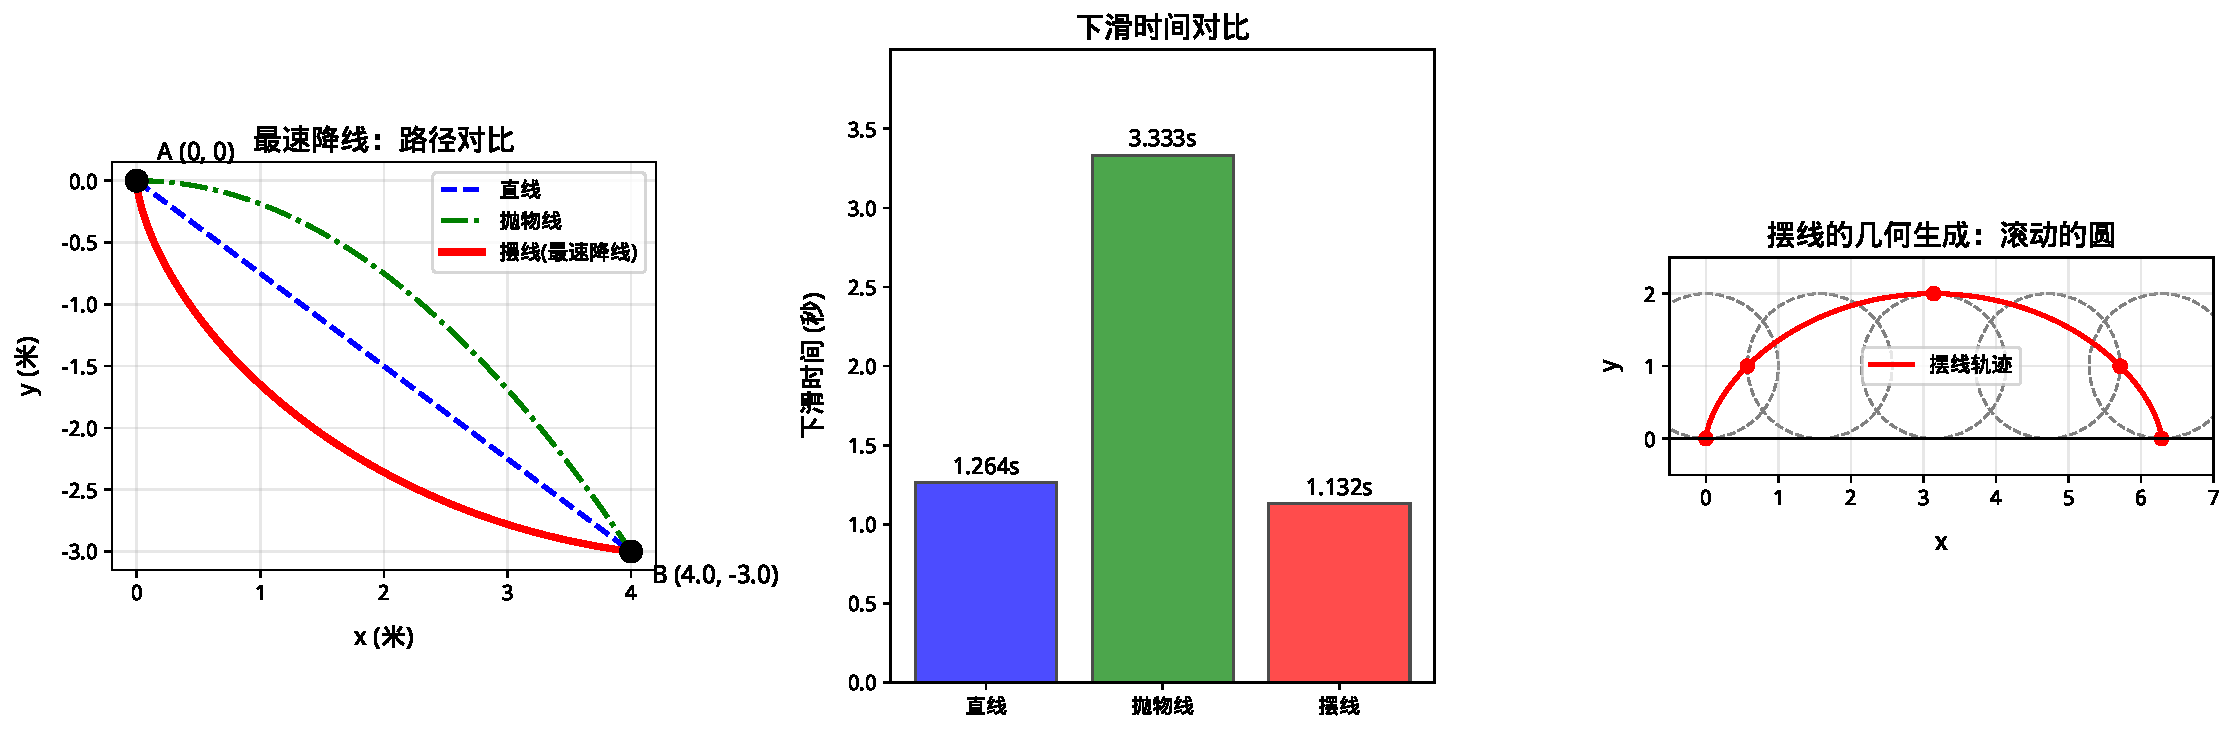
\includegraphics[width=0.95\textwidth]{figs_chap03/brachistochrone.pdf}
\caption{最速降线（Brachistochrone）问题演示。左图对比三种下滑路径：直线、抛物线和摆线；中图显示下滑时间对比——摆线确实是最快的，比直线快约10.5\%；右图展示摆线的几何生成原理：圆在直线上滚动，圆周上一点的轨迹即为摆线。}
\label{fig:chap03_brachistochrone}
\end{figure}

\begin{figure}[htbp]
\centering
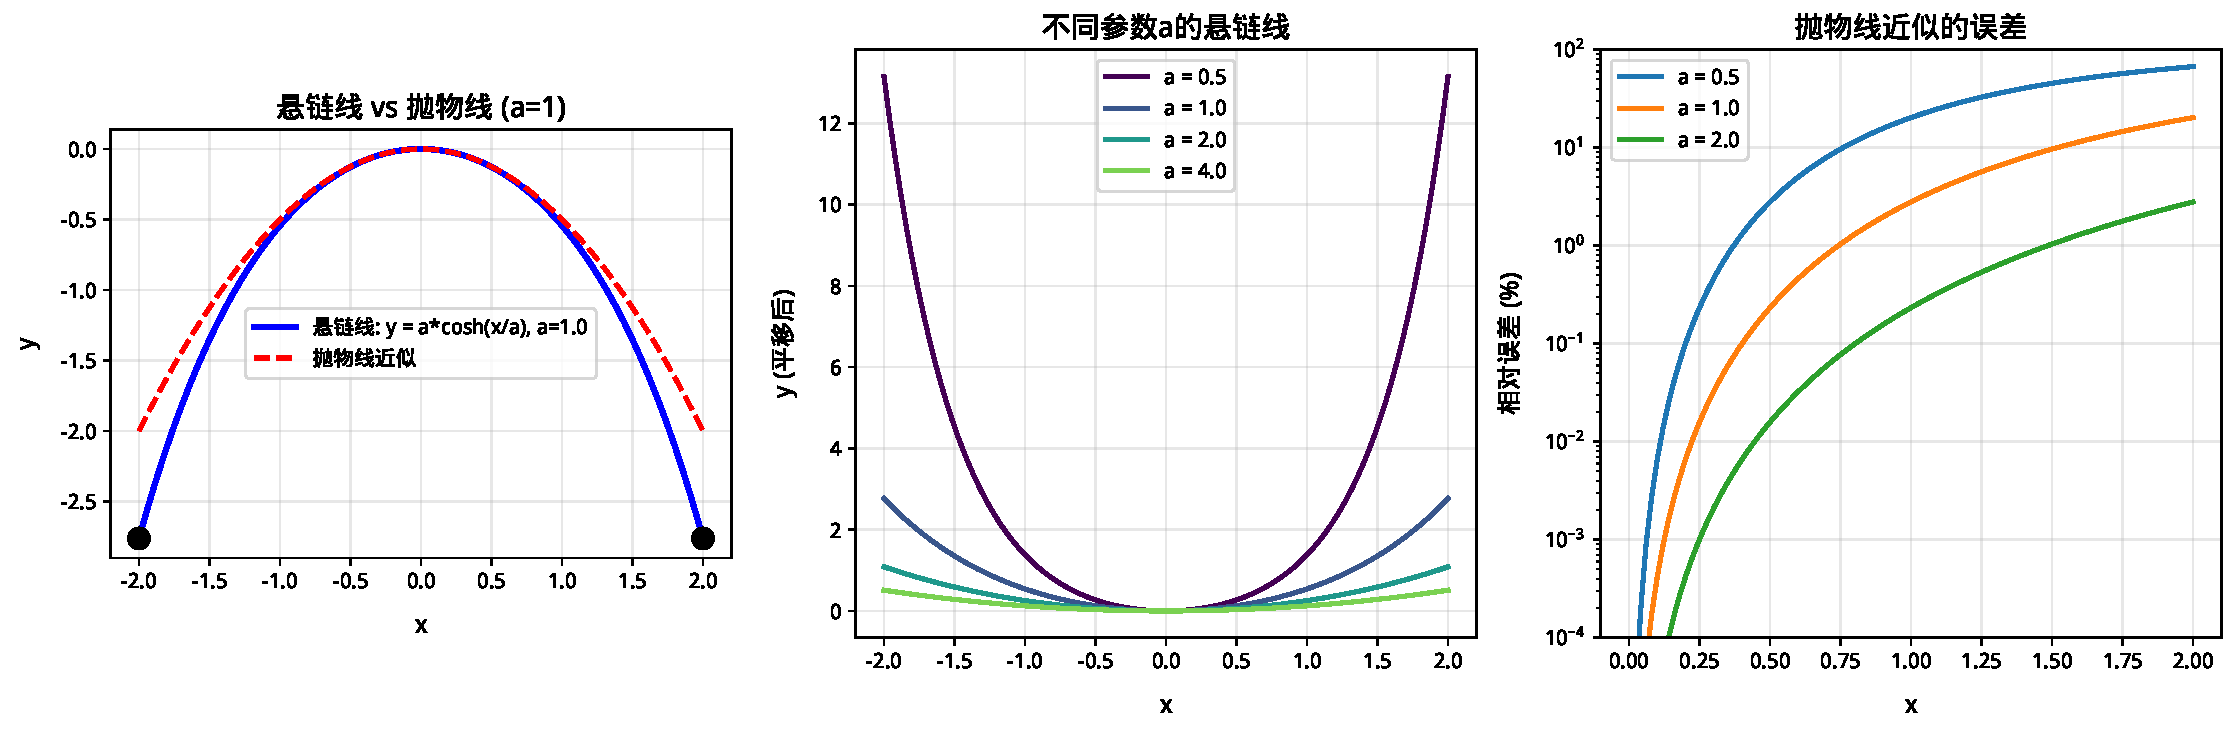
\includegraphics[width=0.95\textwidth]{figs_chap03/catenary.pdf}
\caption{悬链线问题演示。左图对比悬链线$y = a\cosh(x/a)$与抛物线近似（$a=1$时）——两者在中心区域接近，边缘处差异明显；中图展示不同$a$值对悬链线形状的影响——$a$越小，曲线越"尖"；右图显示抛物线近似的相对误差，说明在$|x|$较大时近似失效。}
\label{fig:chap03_catenary}
\end{figure}

% ------------------------------------------------------------------------------------
\section{本章小结}

\begin{enumerate}
    \item \textbf{泛函}：以函数为输入、数字为输出的映射。变分问题就是优化泛函。
    
    \item \textbf{核心观点}：变分法 = 无限维的拉格朗日乘子法。通过离散化，变分问题变成第1章的带约束优化问题。
    
    \item \textbf{Euler-Lagrange 方程}：泛函极值的必要条件
    \[
    \frac{\partial F}{\partial y} - \frac{d}{dx}\frac{\partial F}{\partial y'} = 0
    \]
    
    \item \textbf{守恒律}：
    \begin{itemize}
        \item $F$ 不含 $y$ $\Rightarrow$ $\frac{\partial F}{\partial y'}$ 守恒
        \item $F$ 不含 $x$ $\Rightarrow$ $F - y'\frac{\partial F}{\partial y'}$ 守恒（能量守恒）
    \end{itemize}
    
    \item \textbf{带约束的变分}：用拉格朗日乘子处理积分约束，和第1章方法完全一致。
    
    \item \textbf{经典例子}：
    \begin{itemize}
        \item 测地线（最短路径）→ 直线
        \item 悬链线（最小势能）→ $y = a\cosh(x/a)$
        \item 等周问题（最大面积）→ 圆
    \end{itemize}
\end{enumerate}

\begin{unification}[title=统一视角]
\begin{center}
\renewcommand{\arraystretch}{1.4}
\begin{tabular}{lll}
\toprule
& \textbf{有限维（第1章）} & \textbf{无限维（本章）} \\
\midrule
变量 & 向量 $\mathbf{x} \in \mathbb{R}^n$ & 函数 $y(x)$ \\
目标 & 函数 $f(\mathbf{x})$ & 泛函 $J[y]$ \\
约束 & $g(\mathbf{x}) = 0$ & $y_{k+1} - y_k = v_k \Delta x$ \\
乘子 & $\lambda$ & $\lambda_k = \frac{\partial F}{\partial v_k}$（动量） \\
必要条件 & $\nabla f + \lambda \nabla g = 0$ & E-L 方程 \\
影子价格 & $\frac{df^*}{dc}$ & $\frac{dJ^*}{dc}$（如等周问题中 $\lambda = r$） \\
\bottomrule
\end{tabular}
\end{center}

\textbf{核心洞察}：E-L 方程不是"新发明"，而是有限维乘子法的自然极限。

从下一章开始，我们将用这套语言重新理解自然界：先是"不确定性"（第4章的最大熵），再是牛顿力学与连续介质（第5、13章）——它们都可以看作变分问题！
\end{unification}

% ------------------------------------------------------------------------------------
\section{习题}

\paragraph{计算题}
\begin{enumerate}
    \item 用 E-L 方程求使 $\int_0^1 (y')^2 \, dx$ 最小的函数 $y(x)$，满足 $y(0) = 0$，$y(1) = 1$。
    
    \item 求使 $\int_0^{\pi} [(y')^2 - y^2] \, dx$ 取极值的函数，满足 $y(0) = 0$，$y(\pi) = 0$。
    
    \item 验证悬链线 $y = a\cosh(x/a)$ 满足势能泛函 $J[y] = \int y\sqrt{1+(y')^2} \, dx$ 的 E-L 方程。
    
    \item 用 Beltrami 恒等式（能量守恒）求解最速降线问题：
    \[
    J[y] = \int_0^{x_1} \frac{\sqrt{1+(y')^2}}{\sqrt{y}} \, dx
    \]
    其中 $y$ 向下为正。
\end{enumerate}

\paragraph{证明题}
\begin{enumerate}
    \setcounter{enumi}{4}
    \item 证明：若 $F$ 不显含 $y$，则 $\frac{\partial F}{\partial y'}$ 沿极值曲线为常数。
    
    \item 证明 Beltrami 恒等式：若 $F$ 不显含 $x$，则 $F - y'\frac{\partial F}{\partial y'} = C$。
    
    \item 用离散乘子法证明：对于离散变分问题，$\lambda_k = \frac{\partial F}{\partial v_k}$。（提示：这就是本章第四步）
    
    \item 证明等周问题的拉格朗日乘子 $\lambda$ 等于圆的半径 $r$。
\end{enumerate}

\paragraph{编程题}
\begin{enumerate}
    \setcounter{enumi}{8}
    \item 实现离散变分：
    \begin{enumerate}
        \item 把曲线长度泛函离散化为求和
        \item 用数值优化（如梯度下降）找最短曲线
        \item 验证结果收敛到直线
    \end{enumerate}
    
    \item 数值求解最速降线：
    \begin{enumerate}
        \item 离散化下滑时间泛函
        \item 用优化算法找最优曲线
        \item 与解析解（摆线）比较
        \item 统计时间节省百分比（相比直线）
    \end{enumerate}
    
    \item 实现离散拉格朗日乘子法：
    \begin{enumerate}
        \item 构造离散拉格朗日函数 $\mathcal{L}(\{y_k\}, \{v_k\}, \{\lambda_k\})$
        \item 解 KKT 条件（联立方程组）
        \item 验证 $\lambda_k$ 确实等于 $\frac{\partial F}{\partial v_k}$
    \end{enumerate}
\end{enumerate}

\paragraph{思考题}
\begin{enumerate}
    \setcounter{enumi}{11}
    \item 为什么物理学家喜欢用变分原理（最小作用量）而不是直接用牛顿定律？
    
    \item 本章用"离散化 → 乘子法 → 取极限"推导 E-L 方程。这个思路能否推广到偏微分方程（如波动方程、热传导方程）？
    
    \item 神经网络可以看作是泛函的离散化吗？从这个角度理解物理信息神经网络（PINN）。
    
    \item 机器学习中的"正则化"（如 $L_2$ 正则化）和变分问题中的"光滑性泛函"有什么联系？
\end{enumerate}  % 第3章：变分法

% ####################################################################################
%                              第二部分：物理应用
% ####################################################################################

\part{物理世界中的约束优化}

% ====================================================================================
\chapter{信息与编码：最大熵原理}
% ====================================================================================

\section*{从猜数字游戏说起}

假设我心里想了一个1到8之间的整数，你要用“是/否”问题来猜出它。

\textbf{策略A}（逐个问）：
\begin{quote}
“是1吗？” → 否 → “是2吗？” → 否 → $\cdots$
\end{quote}
最坏情况需要7次。

\textbf{策略B}（二分法）：
\begin{quote}
“大于4吗？” → 是 → “大于6吗？” → 否 → “是5吗？” → 否 → “是6！”
\end{quote}
无论如何只需要3次。

为什么是3次？因为 $\log_2 8 = 3$。每个“是/否”问题最多能把可能性减半，8种可能性需要 $\log_2 8 = 3$ 次二分。

\begin{insightbox}
这个简单的游戏揭示了信息论的核心思想：\textbf{信息量 = 消除不确定性所需的最少问题数}。

Shannon把这个“问题数”叫做\textbf{比特（bit）}——1 bit就是一个“是/否”问题能传递的信息量。
\end{insightbox}

\storynote{Claude Shannon}{1916--2001。他是个有趣的人。他喜欢骑独轮车，会在贝尔实验室的走廊里边骑边抛球杂耍。他发明了“bit”这个词，建立了整个信息论学科。业余时间，他炒股赚了很多钱，还造了各种稀奇古怪的机器。}

\vspace{0.5cm}
\noindent\textit{为什么压缩文件有极限？为什么分类网络的最后一层非用 softmax 不可？为什么“我只知道平均值”这一句话，就足以推出整个分布？}

\begin{quote}
\textbf{本章目标}：你会发现，“信息”这个日常概念可以被精确量化，而计算最大熵分布的方法，正是我们在第1章学过的拉格朗日乘子法！逻辑回归、softmax函数、交叉熵损失，都可以从最大熵原理推导出来。
\end{quote}

\begin{tcolorbox}[colback=green!5, colframe=green!60!black, title=学完这章，你将能够...]
\begin{itemize}
    \item 计算离散分布和连续分布的熵
    \item 用拉格朗日乘子法推导最大熵分布（如指数分布、正态分布）
    \item 解释为什么机器学习用交叉熵作为损失函数
    \item 从最大熵原理推导softmax函数和逻辑回归
    \item 理解KL散度、交叉熵与最大似然之间的关系
\end{itemize}
\end{tcolorbox}

% ------------------------------------------------------------------------------------
\section{信息量的直觉}

\subsection{什么消息更有“信息量”？}

要把“信息”变成一个可以计算的量，先得弄清楚它到底和什么有关。比较两条消息：消息A说“明天太阳从东边升起”，消息B说“明天北京下雪”（假设现在是7月）。哪条消息的信息量更大？直觉告诉我们是消息B，因为消息A是必然发生的事（概率 $\approx 1$），听了等于没听；而消息B是罕见事件（概率很小），一旦成真就大大改变了我们对明天的预期。于是信息量应当是概率的减函数——概率越小，消息越“值钱”。

\begin{keyformula}[title=单个事件的信息量]
事件 $x$ 的信息量（自信息）定义为：
\begin{equation}
I(x) = -\log_2 p(x) \quad \text{（单位：比特）}
\end{equation}
\end{keyformula}
\clarify{这里$p(x)$是事件$x$发生的概率。概率是0到1之间的数，表示事件发生的可能性。比如“抛硬币正面朝上”的概率是0.5，“太阳从东边升起”的概率是1。}

用几个例子验证这个定义是否符合直觉。必然事件（$p=1$）的信息量是 $I = -\log_2 1 = 0$ 比特，没有新信息；抛硬币得到正面（$p=0.5$）的信息量是 $I = -\log_2 0.5 = 1$ 比特；掷骰子得到 6（$p=1/6$）的信息量是 $I = -\log_2(1/6) \approx 2.58$ 比特；一个概率为 $0.001$ 的罕见事件则携带 $I = -\log_2 0.001 \approx 10$ 比特。概率每减半，信息量恰好增加一比特。

\begin{physicalmeaning}
为什么偏偏是 $-\log p$，而不是别的减函数？因为除了“概率越小，信息量越大”（$-\log$ 是单调递减函数）之外，我们对信息量还有两条要求。其一，独立事件的信息量应当可加：同时得知两件互不相关的事，得到的信息应等于分别得知它们的信息之和，而独立事件的概率是相乘的，$I(x \cap y) = -\log(p_x p_y) = -\log p_x - \log p_y = I(x) + I(y)$，对数恰好把乘法变成加法。其二，确定事件的信息量应为零，而 $-\log 1 = 0$。这三条性质唯一地确定了 $-\log p$ 的形式！
\end{physicalmeaning}

\subsection{回到猜数字游戏}

现在我们可以理解为什么猜1-8的数字需要3比特：

每个数字的概率是 $p = 1/8$，信息量是：
\[
I = -\log_2 \frac{1}{8} = \log_2 8 = 3 \text{ 比特}
\]

\textbf{推广}：猜 $n$ 个等可能事件中的一个，需要 $\log_2 n$ 比特。

% ------------------------------------------------------------------------------------
\section{熵：平均信息量}

\subsection{不均匀概率的情况}

猜数字游戏里每个答案等可能，所以每条消息的信息量都一样。现实中的消息源却往往不均匀：假设天气预报说晴天概率 70\%、雨天概率 30\%。如果告诉你“明天是晴天”，信息量是 $-\log_2 0.7 \approx 0.51$ 比特；如果告诉你“明天下雨”，信息量是 $-\log_2 0.3 \approx 1.74$ 比特。两种消息的信息量不同，那么\textbf{平均来看}，每天的天气消息能带来多少信息？自然的做法是按概率加权：

\begin{align}
\text{平均信息量} &= 0.7 \times (-\log_2 0.7) + 0.3 \times (-\log_2 0.3) \\
&= 0.7 \times 0.51 + 0.3 \times 1.74 \\
&\approx 0.88 \text{ 比特}
\end{align}

这个“平均信息量”就是\textbf{熵}。香农 1948 年在《通信的数学理论》里引入这个量时，据说是冯·诺伊曼建议他把它叫作“熵”，理由之一是“没人真正知道熵是什么，所以辩论时你总占上风”。名字的来历下一节会讲清楚——它确实和物理学里的熵是同一个东西。

\begin{keyformula}[title=熵（Shannon Entropy）]
\begin{equation}
H(p) = -\sum_{i=1}^{k} p_i \log_2 p_i = \mathbb{E}[-\log_2 p(X)]
\end{equation}

熵 = 信息量的期望 = 平均每次观测带来的“惊讶程度”
\end{keyformula}
\clarify{$\mathbb{E}[\cdot]$表示“期望”，就是加权平均。如果你没学过概率论，只需记住：期望 = $\sum_i p_i \times (\text{第}i\text{个值})$，即每个值乘以它的概率再求和。}

\subsection{熵的计算例子}

\begin{example}[抛硬币]
公平硬币：$p(\text{正}) = p(\text{反}) = 0.5$
\[
H = -0.5 \log_2 0.5 - 0.5 \log_2 0.5 = 0.5 + 0.5 = 1 \text{ 比特}
\]

不公平硬币：$p(\text{正}) = 0.9$，$p(\text{反}) = 0.1$
\[
H = -0.9 \log_2 0.9 - 0.1 \log_2 0.1 \approx 0.14 + 0.33 = 0.47 \text{ 比特}
\]

\textbf{结论}：越不公平的硬币，熵越小，结果越“可预测”。
\end{example}

\begin{example}[掷骰子]
公平骰子：$p_i = 1/6$
\[
H = -6 \times \frac{1}{6} \log_2 \frac{1}{6} = \log_2 6 \approx 2.58 \text{ 比特}
\]

作弊骰子（6的概率是50\%，其他各10\%）：
\[
H = -0.5 \log_2 0.5 - 5 \times 0.1 \log_2 0.1 \approx 0.5 + 1.66 = 2.16 \text{ 比特}
\]
\end{example}

\subsection{熵的性质}

\begin{figure}[htbp]
\centering
\begin{tikzpicture}[scale=1.2]
    \begin{axis}[
        xlabel={$p$（正面概率）},
        ylabel={$H(p)$（比特）},
        xmin=0, xmax=1,
        ymin=0, ymax=1.1,
        samples=100,
        domain=0.001:0.999,
        grid=major,
        width=10cm,
        height=6cm,
    ]
    \addplot[very thick, blue] {-x*ln(x)/ln(2) - (1-x)*ln(1-x)/ln(2)};
    
    % 标注最大值点
    \addplot[only marks, mark=*, mark size=3pt, red] coordinates {(0.5, 1)};
    \node[above right, red] at (axis cs:0.5, 0.8) {最大值 $H=1$};
    
    % 标注两端
    \node[below] at (axis cs:0, 0) {\small 确定反面};
    \node[below] at (axis cs:1, 0) {\small 确定正面};
    \end{axis}
\end{tikzpicture}
\caption{二元熵函数 $H(p) = -p\log_2 p - (1-p)\log_2(1-p)$。当 $p=0.5$ 时熵最大，当 $p=0$ 或 $p=1$ 时熵为零。}
\end{figure}

从定义可以直接读出熵的三条基本性质。第一是非负性：$H(p) \geq 0$，等号当且仅当某个 $p_i = 1$，也就是结果完全确定时。第二是最大值：对于 $k$ 个可能结果，$H \leq \log_2 k$，等号当且仅当分布均匀——二元熵函数 $H(p)$ 的曲线在 $p = 0.5$ 处取到最大值 1 比特，正是这条性质最简单的情形。第三是可加性：独立系统的熵等于各部分熵之和，
\[
H(X, Y) = H(X) + H(Y) \quad \text{（若 $X, Y$ 独立）}
\]
这一条直接继承自信息量的可加性。

\begin{insightbox}
同一个量 $H(p)$ 可以从三个角度理解，它们说的是一回事：作为\textbf{不确定性}，熵越大，结果越难预测；作为\textbf{信息量}，熵越大，每次观测带来的平均信息越多；作为\textbf{均匀程度}，熵越大，分布越“平坦”。本章后面的最大熵原理用的主要是第三种理解。
\end{insightbox}

% ------------------------------------------------------------------------------------
\section{熵的组合学起源}

\subsection{微观态计数}

上一节把熵定义成平均信息量，但这个定义看上去仍有几分人为：为什么恰好是 $-\sum p \ln p$，而不是别的某个衡量“平坦程度”的函数？答案来自物理学，而且来自一个纯粹的计数问题。

\textbf{问题}：把 $N$ 个可区分的球放入 $k$ 个盒子，第 $i$ 个盒子有 $n_i$ 个球（$\sum_i n_i = N$）。有多少种放法？

答案是多项式系数：
\begin{equation}
W = \frac{N!}{n_1! n_2! \cdots n_k!}
\end{equation}

\begin{example}[具体计算]
把6个球放入3个盒子，分布为 $(3, 2, 1)$：
\[
W = \frac{6!}{3! \cdot 2! \cdot 1!} = \frac{720}{6 \cdot 2 \cdot 1} = 60 \text{ 种}
\]

如果分布为 $(2, 2, 2)$（均匀）：
\[
W = \frac{6!}{2! \cdot 2! \cdot 2!} = \frac{720}{8} = 90 \text{ 种}
\]

均匀分布有更多的微观实现方式！
\end{example}

\subsection{从计数到熵}

当 $N$ 很大时，用 Stirling 近似 $\ln n! \approx n \ln n - n$：
\clarify{从这里开始，我们改用自然对数 $\ln$（单位是奈特 nat），它与 $\log_2$（比特）只差常数 $\ln 2$。凡是与比特有关的地方（编码、压缩）会再换回 $\log_2$。}

令 $p_i = n_i / N$（各盒子的比例），则：
\begin{align}
\frac{1}{N} \ln W &= \frac{1}{N} \left( \ln N! - \sum_i \ln n_i! \right) \\
&\approx \frac{1}{N} \left( N \ln N - N - \sum_i (n_i \ln n_i - n_i) \right) \\
&= \ln N - \sum_i \frac{n_i}{N} \ln n_i \\
&= -\sum_i p_i \ln p_i
\end{align}

（最后一步用到 $\ln n_i = \ln(p_i N) = \ln p_i + \ln N$）

于是，香农的熵不是凭空定义的：它就是微观态数的对数按球数平摊后的值。这也回答了前面的疑问——$-\sum p \ln p$ 这个形式是从计数里长出来的，不是选出来的。

\begin{keytheorem}[title=熵的组合学意义]
\begin{equation}
H(p) = -\sum_i p_i \ln p_i \approx \frac{1}{N} \ln W
\end{equation}

\textbf{熵 $\propto$ 微观态数的对数}

熵大 $\Leftrightarrow$ 微观实现方式多 $\Leftrightarrow$ 更“自然”、更容易出现
\end{keytheorem}
\storynote{Ludwig Boltzmann}{1844--1906，奥地利物理学家，统计力学奠基人。他的墓碑上刻着$S = k \log W$——熵等于微观态数的对数。这个公式连接了宏观热力学和微观统计力学。他因学术争论而抑郁，最终自杀，但他的理论被后世完全证实。}

\begin{physicalmeaning}
想象把一盒气体分子放到房间里。所有分子挤在角落是低熵状态，只有极少数微观态对应这种宏观状态；分子均匀分布在房间是高熵状态，有海量微观态与之对应。这就是为什么气体会自发扩散——不是因为有什么“力”推动，而是因为均匀分布对应的微观态数压倒性地多！
\end{physicalmeaning}

% ------------------------------------------------------------------------------------
\section{最大熵原理}

\subsection{一个关键问题}

前两节回答了“熵是什么”。现在把问题反过来：能不能用熵去\textbf{构造}分布？假设你在调查某城市的收入分布，但只知道两个信息——平均收入是 5 万元，而且收入必须非负。你应该假设什么样的收入分布？

\begin{figure}[htbp]
\centering
\begin{tikzpicture}[scale=0.9]
    \begin{axis}[
        xlabel={收入（万元）},
        ylabel={概率密度},
        xmin=0, xmax=20,
        ymin=0, ymax=0.25,
        samples=100,
        domain=0:20,
        width=12cm,
        height=6cm,
        legend pos=north east,
    ]
    % 指数分布（最大熵）
    \addplot[very thick, blue] {0.2*exp(-0.2*x)};
    \addlegendentry{指数分布（最大熵）}
    
    % 其他可能的分布
    \addplot[thick, red, dashed] {0.4*x*exp(-0.4*x)};
    \addlegendentry{其他分布1}
    
    \addplot[thick, green!60!black, dotted] {1/(5*sqrt(2*pi))*exp(-(x-5)^2/50)};
    \addlegendentry{其他分布2}
    \end{axis}
\end{tikzpicture}
\caption{满足“均值=5万”约束的不同分布。哪个是“最合理”的选择？}
\end{figure}

有无穷多个分布满足“均值=5万”的条件。选哪一个？

\subsection{最大熵原理的回答}

\begin{quote}
\textit{“不要假装知道你不知道的东西。在约束条件下，选择最均匀（熵最大）的分布。”}
\end{quote}

\begin{keyformula}[title=最大熵原理]
在所有满足已知约束的分布中，选择\textbf{熵最大}的那个。

数学形式：
\begin{equation}
\max_{p} \quad H(p) = -\sum_i p_i \ln p_i
\end{equation}
\begin{align}
\text{s.t.} \quad & \sum_i p_i = 1 \quad \text{（归一化）} \\
& \sum_i p_i g_j(x_i) = c_j, \quad j = 1, \ldots, m \quad \text{（已知约束）}
\end{align}
\end{keyformula}

为什么这是合理的？可以从三个角度回答。从组合学看，上一节的计数表明最大熵分布对应最多的微观态，是“最可能”的宏观状态；从信息论看，最大熵就是最大不确定性，意味着除了已知约束之外不引入任何额外假设；从决策论看，如果你用错误的分布做决策，最大熵分布让你的“最坏情况损失”最小。三条理由指向同一个结论：只知道部分信息时，最大熵分布是最诚实的选择。

\storynote{Edwin Jaynes}{1922--1998，美国物理学家，最大熵原理的现代奠基人。他1957年的论文将熵和概率推理统一起来，影响了统计学、机器学习、贝叶斯推断等领域。他认为``概率是知识的逻辑，不是物理的性质''。}

\begin{tcolorbox}[colback=yellow!10, colframe=orange!80, title=本章的核心观点]
\textbf{最大熵原理不是什么新东西——它就是第1章的拉格朗日乘子法，只不过“变量”从一个向量 $x$ 变成了一个概率分布 $p$，“目标”从某个代价变成了熵。}

约束是什么？——你\textbf{已知}的东西：概率必须归一化，某些量的平均值必须等于观测值。

乘子是什么？——每条已知信息的“熵价格”：$\beta_j = -\partial H^*/\partial c_j$。在物理里它给出温度的倒数，在机器学习里它是特征权重 $w_j$。这不是巧合。

\begin{center}
\renewcommand{\arraystretch}{1.3}
\small
\begin{tabularx}{\linewidth}{llX}
\toprule
 & \textbf{第1章（约束优化）} & \textbf{本章（最大熵）} \\
\midrule
变量 & 向量 $x \in \R^n$ & 分布 $p = (p_1, \ldots, p_k)$ 或密度 $p(x)$ \\
目标 & $\min f(x)$ & $\max H(p) = -\sum_i p_i \ln p_i$ \\
约束 & $g(x) = 0$ & $\sum_i p_i = 1$，$\sum_i p_i g_j(x_i) = c_j$ \\
乘子 & $\lambda$ & $\alpha$（给出配分函数 $Z$），$\beta_j$（特征权重 / 逆温度） \\
一阶条件 & $\nabla f + \lambda \nabla g = 0$ & $-\ln p_i - 1 + \alpha + \sum_j \beta_j g_j(x_i) = 0$ \\
解 & 驻点 $x^*$ & 指数族 $p_i = e^{\sum_j \beta_j g_j(x_i)} / Z$ \\
影子价格 & $\lambda = -df^*/d\epsilon$ & $\beta_j = -\partial H^*/\partial c_j$ \\
\bottomrule
\end{tabularx}
\end{center}
\end{tcolorbox}

\subsection{用拉格朗日乘子法求解}

这是一个带等式约束的优化问题——正是第1章拉格朗日乘子法的舞台！
\review{第1章}{拉格朗日函数 $\Lag = f + \lambda^\top g$，对所有变量（包括乘子）求导令其为零。这里 $f = -H(p)$（最小化负熵），$g$ 是归一化和矩约束，每个约束配一个乘子——本章把它们记作 $\alpha$ 和 $\beta_j$，以免与指数分布的率参数 $\lambda$ 混淆。}

\paragraph{Step 1：构造拉格朗日函数}
\begin{equation}
\mathcal{L}(p, \alpha, \bm{\beta}) = -\sum_i p_i \ln p_i + \alpha\left(\sum_i p_i - 1\right) + \sum_{j=1}^{m} \beta_j \left(\sum_i p_i g_j(x_i) - c_j\right)
\end{equation}

\paragraph{Step 2：对 $p_i$ 求导并令其为零}
\begin{equation}
\frac{\partial \mathcal{L}}{\partial p_i} = -\ln p_i - 1 + \alpha + \sum_j \beta_j g_j(x_i) = 0
\end{equation}

\paragraph{Step 3：解出 $p_i$}
\begin{equation}
\ln p_i = \alpha - 1 + \sum_j \beta_j g_j(x_i)
\end{equation}

\begin{equation}
p_i = \exp\left( \alpha - 1 + \sum_j \beta_j g_j(x_i) \right)
\end{equation}

\paragraph{Step 4：用归一化条件确定 $\alpha$}

由 $\sum_i p_i = 1$，定义配分函数：
\review{第2章}{“$\beta$ 的值由约束隐式确定”其实就是在解对偶问题：$\min_\beta [\ln Z(\beta) - \beta^\top c]$。它无约束、且是凸的（log-sum-exp 减线性），对 $\beta_j$ 求导恰好得到 $\langle g_j \rangle = c_j$。}
\begin{equation}
Z(\bm{\beta}) = \sum_i \exp\left( \sum_j \beta_j g_j(x_i) \right)
\end{equation}

则 $e^{\alpha - 1} = 1/Z$，最终得到：

\begin{keytheorem}[title=最大熵分布的指数形式]
\begin{equation}
\boxed{p_i = \frac{1}{Z} \exp\left( \sum_j \beta_j g_j(x_i) \right)}
\label{eq:maxent}
\end{equation}

其中 $Z = \sum_i \exp\left( \sum_j \beta_j g_j(x_i) \right)$ 是归一化常数（配分函数），$\beta_j$ 是约束 $\langle g_j \rangle = c_j$ 对应的拉格朗日乘子，它的值由约束条件隐式确定。
\end{keytheorem}
\preview{这个“指数族”形式就是深度学习里的 softmax：第8章分类网络的输出层、第11章 Transformer 的注意力权重 $\mathrm{softmax}(q \cdot k / \sqrt{d})$ 都是它的实例，第11章还会把 $\sqrt{d}$ 解释成“温度”。}

\begin{physicalmeaning}
拉格朗日乘子 $\beta_j$ 做的事情是调节分布的形状，使得约束 $\langle g_j \rangle = c_j$ 被精确满足：$\beta_j > 0$ 时，分布倾向于让 $g_j(x)$ 大的状态概率增加；$\beta_j < 0$ 时则相反，倾向于让 $g_j(x)$ 大的状态概率减少。

在物理中，取 $g = E$（能量）时得到玻尔兹曼分布 $p \propto e^{-E/kT}$，即 $\beta = -1/kT$（物理惯例把乘子取相反符号），$|\beta|$ 是逆温度；在机器学习中，$\beta$ 是特征权重。E. T. Jaynes 1957 年提出最大熵原理时，正是把统计力学整个解释成这样一种在已知约束下的推断：玻尔兹曼分布不是额外的物理假设，而是“只知道平均能量”时的最大熵解。

更准确地说：$\beta_j = -\dfrac{\partial H^*}{\partial c_j}$——它度量“多知道一点信息（约束值变一个单位），最大熵下降多少”。这与第1章的 $\lambda = -df^*/d\epsilon$ 完全对应：从“影子价格”到“特征权重”，$\lambda$ 的统一性再次显现！
\end{physicalmeaning}

% ------------------------------------------------------------------------------------
\section{经典分布的推导}

有了式~\eqref{eq:maxent}，推导一个具体的分布就只剩两步：说清楚约束是什么，再由约束把乘子定出来。下面用这套程序推导几个著名的概率分布，约束一次比一次多。
\clarify{如果你没学过概率论，不用担心——本节推导的这些分布（均匀分布、指数分布、高斯分布）是最基础的概率分布，学完本节你就掌握了概率论最核心的几个分布！}

\subsection{均匀分布：一无所知时}

这时唯一的约束是归一化 $\sum_i p_i = 1$，拉格朗日函数只需要一个乘子：
\begin{equation}
\mathcal{L} = -\sum_i p_i \ln p_i + \alpha \left( \sum_i p_i - 1 \right)
\end{equation}

\begin{equation}
\frac{\partial \mathcal{L}}{\partial p_i} = -\ln p_i - 1 + \alpha = 0 \quad \Rightarrow \quad p_i = e^{\alpha - 1}
\end{equation}

由于右边不依赖于 $i$，所以 $p_i$ 对所有 $i$ 相同：
\begin{equation}
\boxed{p_i = \frac{1}{k}} \quad \text{（均匀分布）}
\end{equation}

\begin{insightbox}
当你对一件事\textbf{一无所知}时（没有任何约束），最大熵原理告诉你：\textbf{假设每种可能性相等}。

这就是概率论中的“无差别原理”或“不充分理由原则”。
\end{insightbox}

\subsection{指数分布：已知均值时}

现在多知道一点：变量非负，而且均值已知。约束因此有三条——归一化 $\int_0^\infty p(x) dx = 1$，均值 $\int_0^\infty x \cdot p(x) dx = \mu$，以及支撑 $x \geq 0$（它决定了积分区间）。其中只有一个“矩约束” $g(x) = x$，$c = \mu$。

由最大熵公式：
\begin{equation}
p(x) = \frac{1}{Z} e^{\beta x}
\end{equation}

为了让 $p(x)$ 在 $[0, \infty)$ 上可积，必须 $\beta < 0$。令 $\lambda = -\beta > 0$：
\clarify{这里的 $\lambda = -\beta$ 只是指数分布的率参数（rate），和第1章的乘子 $\lambda$ 不是一回事——本章的乘子记作 $\alpha$、$\beta_j$。}
\begin{equation}
p(x) = \frac{1}{Z} e^{-\lambda x}
\end{equation}

计算归一化常数：
\begin{equation}
Z = \int_0^\infty e^{-\lambda x} dx = \frac{1}{\lambda}
\end{equation}

计算均值约束：
\begin{equation}
\mu = \int_0^\infty x \cdot \lambda e^{-\lambda x} dx = \frac{1}{\lambda}
\end{equation}

所以 $\lambda = 1/\mu$，最终得到：

\begin{equation}
\boxed{p(x) = \frac{1}{\mu} e^{-x/\mu}} \quad \text{（指数分布）}
\end{equation}

\begin{physicalmeaning}
指数分布在放射性衰变（已知平均寿命）、电话呼叫的到达间隔（已知平均间隔）、设备的故障时间（已知平均寿命）里反复出现。这些情况的共同特点是只知道均值，不知道其他信息；最大熵原理告诉我们，这时就应该假设指数分布。
\end{physicalmeaning}
\think{按第1章“影子价格”的定义，$\beta_j$ 应该等于哪个导数？提示：把最优熵 $H^*$ 看成 $c_j$ 的函数，用包络定理，你会得到 $\beta_j = -\partial H^*/\partial c_j$。热力学里 $\partial S/\partial U = 1/T$——温度的倒数正是“能量约束的影子价格”。}

\subsection{高斯分布：已知均值和方差时}

再多知道一点：均值 $\mu$ 和方差 $\sigma^2$ 都已知，支撑是整个实轴。约束是归一化 $\int_{-\infty}^{\infty} p(x) dx = 1$、均值 $\int x \cdot p(x) dx = \mu$ 和方差 $\int (x-\mu)^2 \cdot p(x) dx = \sigma^2$，也就是两个矩约束 $g_1(x) = x$，$g_2(x) = (x-\mu)^2$。

由最大熵公式：
\begin{equation}
p(x) = \frac{1}{Z} \exp\left( \beta_1 x + \beta_2 (x-\mu)^2 \right)
\end{equation}

为了可积，$\beta_2 < 0$。令 $\beta_2 = -1/(2\sigma^2)$，可以验证均值约束要求 $\beta_1 = 0$（因为 $(x-\mu)^2$ 已经以 $\mu$ 为中心）。

最终：
\begin{equation}
\boxed{p(x) = \frac{1}{\sqrt{2\pi\sigma^2}} \exp\left( -\frac{(x-\mu)^2}{2\sigma^2} \right)} \quad \text{（高斯分布）}
\end{equation}
\storynote{高斯}{高斯（1777-1855）被誉为“数学王子”。高斯分布以他命名，但最早是德莫瓦弗在1733年发现的。高斯用它来分析天文观测误差，发现它神奇地描述了几乎所有测量误差的分布。}

\begin{keytheorem}[title=高斯分布的最大熵性质]
在所有均值为 $\mu$、方差为 $\sigma^2$ 的连续分布中，\textbf{高斯分布的熵最大}。

这解释了为什么高斯分布在自然界和统计学中如此普遍——当你只知道均值和方差时，高斯分布是“最诚实”的选择。
\end{keytheorem}

\subsection{经典分布总结}

\begin{center}
\renewcommand{\arraystretch}{1.5}
\begin{tabular}{l|l|l}
\toprule
\textbf{已知约束} & \textbf{最大熵分布} & \textbf{应用场景} \\
\midrule
仅归一化 & 均匀分布 & 完全无知 \\
均值（离散有限） & 几何分布 & 等待时间 \\
均值（连续非负） & 指数分布 & 寿命、间隔 \\
均值 + 方差 & 高斯分布 & 测量误差、自然现象 \\
均值（非负整数） & 泊松分布 & 计数数据 \\
\bottomrule
\end{tabular}
\end{center}
\tryit{用 numpy 各生成 10 万个均值 0、方差 1 的样本（高斯、均匀 $[-\sqrt{3}, \sqrt{3}]$、拉普拉斯），用直方图估计熵，验证高斯最大：理论值分别约 1.42、1.24、1.35 nat。}

% ------------------------------------------------------------------------------------
\section{KL散度：分布之间的“距离”}

\subsection{问题的提出}

到目前为止我们只谈单个分布的熵。但机器学习里更常见的情形是手里有两个分布，需要比较它们的“差异”：模型预测的分布 $q$ 与真实分布 $p$ 有多接近？数据的经验分布与理论分布差多少？一个自然的想法是用“距离”来度量。但什么样的“距离”对概率分布是合理的？

\subsection{KL散度的定义}

\begin{keyformula}[title=KL散度（Kullback-Leibler Divergence）]
\begin{equation}
D_{KL}(P \| Q) = \sum_i p_i \ln \frac{p_i}{q_i} = \sum_i p_i \ln p_i - \sum_i p_i \ln q_i
\end{equation}

或写成期望形式：
\begin{equation}
D_{KL}(P \| Q) = \mathbb{E}_{x \sim P} \left[ \ln \frac{P(x)}{Q(x)} \right]
\end{equation}
\end{keyformula}
\preview{KL散度是深度学习中最重要的概念之一。第8章的神经网络训练、第9章的强化学习策略优化、第12章的大模型后训练（RLHF 里的 KL 约束）、第16章的世界模型，都会反复用到它。现在花时间理解透彻，后面会事半功倍！}

\subsection{KL散度的直觉}

\begin{physicalmeaning}
KL散度的三种理解：

\textbf{1. 编码效率损失}

如果真实分布是 $P$，但你用基于 $Q$ 设计的编码，平均每个符号要多用
\[
D_{KL}(P \| Q) = H(P, Q) - H(P)
\]
比特。这是用“错误模型”的代价。

\textbf{2. 信息增益}

当你从“先验” $Q$ 更新到“后验” $P$，获得的信息量是 $D_{KL}(P \| Q)$。

\textbf{3. 统计区分度}

$D_{KL}(P \| Q)$ 越大，越容易通过采样区分 $P$ 和 $Q$。
\end{physicalmeaning}

\subsection{KL散度的性质}

KL散度最重要的性质是\textbf{非负性}：$D_{KL}(P \| Q) \geq 0$。证明只需要 Jensen 不等式和 $\ln$ 的凹性：
\[
-D_{KL}(P \| Q) = \sum_i p_i \ln \frac{q_i}{p_i} \leq \ln \sum_i p_i \cdot \frac{q_i}{p_i} = \ln \sum_i q_i = \ln 1 = 0
\]
进一步，等号当且仅当 $P = Q$ 时成立，即 $D_{KL}(P \| Q) = 0 \Leftrightarrow P = Q$。这两条使 KL散度可以充当分布之间的“距离”。但它并不是真正的距离——一般 $D_{KL}(P \| Q) \neq D_{KL}(Q \| P)$，交换两个分布的位置，结果会变。

\begin{example}[不对称性的例子]
设 $P = (0.5, 0.5)$，$Q = (0.9, 0.1)$。

\begin{align}
D_{KL}(P \| Q) &= 0.5 \ln \frac{0.5}{0.9} + 0.5 \ln \frac{0.5}{0.1} \\
&= 0.5 \times (-0.588) + 0.5 \times 1.609 = 0.51
\end{align}

\begin{align}
D_{KL}(Q \| P) &= 0.9 \ln \frac{0.9}{0.5} + 0.1 \ln \frac{0.1}{0.5} \\
&= 0.9 \times 0.588 + 0.1 \times (-1.609) = 0.37
\end{align}

$D_{KL}(P \| Q) \neq D_{KL}(Q \| P)$！
\end{example}

\begin{insightbox}
KL散度不对称的直觉：

$D_{KL}(P \| Q)$ 衡量“用 $Q$ 近似 $P$”的代价——在 $P$ 概率大的地方，$Q$ 不能太小。

$D_{KL}(Q \| P)$ 衡量“用 $P$ 近似 $Q$”的代价——在 $Q$ 概率大的地方，$P$ 不能太小。

两个方向关心的“重点区域”不同！
\end{insightbox}

\subsection{最大熵 = 最小KL散度}

\begin{unification}[title=最大熵的等价形式]
\begin{equation}
\max_p H(p) \;\text{s.t. 约束} \quad \Longleftrightarrow \quad \min_p D_{KL}(p \| u) \;\text{s.t. 约束}
\end{equation}

其中 $u$ 是均匀分布。

\textbf{最大熵 = 在约束下离均匀分布最近}
\end{unification}
\preview{把这里的均匀分布 $u$ 换成“旧策略”，$\min D_{KL}(p \| u)$ 就变成第9章信任域方法（TRPO/PPO）里“新策略别离旧策略太远”的约束。}

\textit{证明}：
\begin{align}
D_{KL}(p \| u) &= \sum_i p_i \ln \frac{p_i}{1/k} = \sum_i p_i \ln p_i + \sum_i p_i \ln k \\
&= -H(p) + \ln k
\end{align}

由于 $\ln k$ 是常数，$\min D_{KL}(p \| u) \Leftrightarrow \max H(p)$。

\section{KL散度的第一性原理}

\subsection{什么是“好的”分布距离？}

假设我们想用一个简单的分布 $q(x)$ 去近似复杂的真实分布 $p(x)$。我们需要一个“差异度量” $D(p \| q)$ 来衡量近似的好坏。

但是，什么样的度量才是“合理”的？信息论给出了答案：合理的度量必须满足三条公理。

\begin{keyformula}[title={信息距离的三条公理 (Shore \& Johnson, 1980)}]
\begin{enumerate}
    \item \textbf{局部性 (Locality)}：差异应该是逐点累积的，不依赖全局耦合。
    \[
    D(p \| q) = \int f(p(x), q(x)) \, dx
    \]
    
    \item \textbf{可加性 (Additivity)}：对于独立系统 $A, B$，联合分布的差异等于各自差异之和。
    \[
    D(p_A p_B \| q_A q_B) = D(p_A \| q_A) + D(p_B \| q_B)
    \]
    
    \item \textbf{一致性 (Consistency)}：当 $q(x) = p(x)$ 时，差异为零且达到最小值。
\end{enumerate}
\end{keyformula}

\begin{physicalmeaning}
这三条公理各有直觉。局部性说的是每个点的偏差独立计算，就像质量、能量一样是“广延量”；可加性说的是独立系统的总偏差等于各自偏差之和，这与熵、能量的性质一致；一致性说的是完美近似时差异为零——这是最基本的要求。
\end{physicalmeaning}

\subsection{从公理推导KL散度}

\paragraph{Step 1：利用可加性锁定函数形式}

设差异度量为 $D(p\|q) = \sum_i h(p_i, q_i)$。

考虑两个独立事件，联合概率 $p_{ij} = u_i v_j$，$q_{ij} = \alpha_i \beta_j$。根据可加性：
\[
\sum_{i,j} h(u_i v_j, \alpha_i \beta_j) = \sum_i h(u_i, \alpha_i) + \sum_j h(v_j, \beta_j)
\]

这是一个经典的\textbf{柯西函数方程}变体。数学上可以证明，唯一满足此性质的连续函数形式必须包含\textbf{对数项}：
\[
h(p, q) = c \cdot p \ln \frac{p}{q} + \cdots
\]

\paragraph{Step 2：利用一致性确定系数}

设通解为：
\[
D(p\|q) = \int \left( A p(x) \ln p(x) + B p(x) \ln q(x) + C p(x) \right) dx
\]

根据一致性公理：当 $q(x) \to p(x)$ 时，$D$ 必须达到最小值（且为0）。

对 $q(x)$ 求变分导数（考虑归一化约束）：
\[
\frac{\delta}{\delta q} \left( D(p\|q) + \lambda \int q \, dx \right) = 0
\quad \Rightarrow \quad
\frac{B p(x)}{q(x)} + \lambda = 0
\]

为了让最优解是 $q^*(x) = p(x)$、且 $D(p\|p) = 0$，需要 $A + B = 0$，$B < 0$（极小性）；取归一化 $A = -B = 1$（相当于选定对数底），就得到：

\begin{keytheorem}[title=KL散度的唯一性]
满足局部性、可加性、一致性三条公理的差异度量，在相差一个正常数（即对数底的选择）的意义下是\textbf{唯一}的：
\begin{equation}
\boxed{D_{KL}(p \| q) = \int p(x) \ln \frac{p(x)}{q(x)} \, dx = -H(p) - \int p(x) \ln q(x) \, dx}
\end{equation}
\end{keytheorem}

\begin{insightbox}
\textbf{为什么机器学习中常用交叉熵损失？}

最小化 $D_{KL}(p^* \| q)$ 等价于：
\[
\min_q \left( \underbrace{-H(p^*)}_{\text{常数，与 }q\text{ 无关}} + \underbrace{\left(-\int p^*(x) \ln q(x) \, dx\right)}_{\text{交叉熵 }H(p^*, q)} \right)
\]

因此，\textbf{最小化交叉熵 = 最小化KL散度 = 找最逼近真实分布的模型}。

这不是“选择”，而是\textbf{数学必然}！
\end{insightbox}

% ------------------------------------------------------------------------------------
\section{常见损失函数的“违规记录”}

既然 KL散度是唯一满足三条公理的度量，为什么实践中还有那么多别的损失函数？因为并非所有损失函数都需要满足信息论公理。有些为了特定的工程目的（如鲁棒性、几何感知），故意违反某些公理。

\begin{center}
\renewcommand{\arraystretch}{1.6}
\begin{tabularx}{\textwidth}{p{2.4cm}|p{2.8cm}|p{2cm}|X}
\toprule
\textbf{损失函数} & \textbf{数学形式} & \textbf{违反的公理} & \textbf{为何要违反？} \\
\midrule
\textbf{交叉熵} (Cross Entropy) 
& $-\sum p \ln q$ 
& 无 
& 信息论的“正统”选择 \\
\midrule
\textbf{MSE} (均方误差) 
& $\int (p-q)^2 dx$ 
& 可加性 
& 计算便利，求导简单，适合回归任务 \\
\midrule
\textbf{MAE} (L1 Loss) 
& $\int |p-q| dx$ 
& 可加性 
& 对异常值鲁棒，不被离群点拉偏 \\
\midrule
\textbf{Hinge} (SVM) 
& $\max(0, 1-yf(x))$ 
& 一致性 
& 追求稀疏性和分类边界，不追求估计真实概率 \\
\midrule
\textbf{Wasserstein} (WGAN) 
& $\inf \mathbb{E}[\|x-y\|]$ 
& 局部性 
& 引入空间距离（全局耦合），解决分布不重叠时KL散度梯度消失的问题 \\
\bottomrule
\end{tabularx}
\end{center}

\begin{physicalmeaning}
\textbf{选择损失函数的智慧}：如果你相信数据服从某个概率模型，就用交叉熵，它是信息论意义下的最优选择；如果你想要对异常值鲁棒，就用 MAE 或 Huber 损失；如果你只关心分类边界，就用 Hinge 损失；如果两个分布可能不重叠，就用 Wasserstein 距离。没有“最好”的损失函数，只有最适合问题的损失函数——每一次“违规”都是在用信息论最优性换取某种工程性质。
\end{physicalmeaning}


% ------------------------------------------------------------------------------------
\section{交叉熵与机器学习}
\preview{本节会出现“神经网络”、“分类器”等深度学习术语。如果你没学过深度学习，暂时只需知道：神经网络是一种能从数据中学习规律的数学模型，分类器是判断“这张图是猫还是狗”之类问题的程序。第8章会详细介绍。}

\subsection{交叉熵的定义}

\begin{keyformula}[title=交叉熵]
\begin{equation}
H(P, Q) = -\sum_i p_i \ln q_i = H(P) + D_{KL}(P \| Q)
\end{equation}

交叉熵 = 真实分布的熵 + KL散度
\end{keyformula}

\subsection{为什么机器学习用交叉熵损失？}

前面的推导都是关于分布本身的，现在把它接到机器学习最常见的任务——分类——上。在分类问题中，$P$ 是真实标签分布（通常是 one-hot，如 $[0, 1, 0]$），$Q$ 是模型预测的概率分布（如 $[0.1, 0.7, 0.2]$）。训练目标是让 $Q$ 尽量接近 $P$，即最小化 $D_{KL}(P \| Q)$。

由于 $H(P)$ 是固定的（真实标签不变），所以：
\begin{equation}
\min_Q D_{KL}(P \| Q) \quad \Longleftrightarrow \quad \min_Q H(P, Q)
\end{equation}

对于 one-hot 标签 $y = [0, \ldots, 1, \ldots, 0]$（第 $c$ 类为1）：
\begin{equation}
H(P, Q) = -\sum_i y_i \ln q_i = -\ln q_c
\end{equation}

这就是我们熟悉的\textbf{交叉熵损失}！

\begin{insightbox}
\textbf{为什么不用均方误差（MSE）？}对于分类问题，交叉熵有三个优势。它是信息论最优的：交叉熵直接度量“用模型编码真实数据”的代价。它的梯度性质好：当预测很错时，交叉熵的梯度大，而 MSE 的梯度可能很小（梯度消失）。它还有概率解释：最小化交叉熵等价于最大化似然。
\end{insightbox}

\subsection{Softmax = 最大熵分布}

神经网络分类器的输出通常经过 softmax 函数：
\begin{equation}
p_i = \frac{e^{z_i}}{\sum_j e^{z_j}}
\end{equation}
\clarify{softmax函数把一组任意实数变成概率分布（全为正数且和为1）。它是深度学习中最常用的函数之一。在第8章你会看到它如何用于图像分类、第11章会看到它如何用于Transformer注意力机制。}

这个形式是不是很眼熟？让我们一步步看它是如何从最大熵原理推导出来的。

\begin{insightbox}
\textbf{Softmax的推导：从最大熵到神经网络}

回顾前面推导的最大熵分布形式（式~\eqref{eq:maxent}）：
\[
p_i = \frac{1}{Z} \exp\left( \sum_j \beta_j g_j(x_i) \right)
\]

现在考虑分类问题：我们想预测输入 $\bm{x}$ 属于哪个类别。

\textbf{Step 1}：神经网络为每个类别 $i$ 计算一个得分（logit）：
\[
z_i = \bm{w}_i^\top \bm{x} + b_i
\]

\textbf{Step 2}：将这个得分代入最大熵分布。这里 $z_i$ 就是 $\sum_j \beta_j g_j(x_i)$ 的具体形式——它表示类别 $i$ 的“能量”或“偏好程度”。

\textbf{Step 3}：归一化得到概率：
\[
p_i = \frac{e^{z_i}}{\underbrace{\sum_j e^{z_j}}_{Z = \text{配分函数}}}
\]

这正是 softmax 函数！
\end{insightbox}

\begin{unification}[title=Softmax的最大熵解释]
Softmax 函数给出的是满足约束 $\langle z \rangle = \sum_i p_i z_i = c$ 的\textbf{最大熵分布}。

其中 $z_i$ 是神经网络的 logits（未归一化得分），$c$ 是由网络参数决定的常数。

\textbf{神经网络学习的权重 $\bm{w}_i$ 是最大熵分布的拉格朗日乘子，logit $z_i = \bm{w}_i^\top \bm{x}$ 是“乘子 $\times$ 特征”。}
\end{unification}

\begin{physicalmeaning}
\textbf{为什么叫 “softmax”？}

考虑一个“硬”版本——argmax，它只输出得分最高的类别：
\[
\text{argmax: } p_i = \begin{cases} 1 & \text{if } i = \arg\max_j z_j \\ 0 & \text{otherwise} \end{cases}
\]

Softmax 是它的“软”版本：当各 $z_i$ 差异很大时，softmax 接近 argmax（赢者通吃）；当各 $z_i$ 差异很小时，softmax 接近均匀分布（不确定）。

你可以通过引入“温度”参数 $T$ 来控制软硬程度：
\[
p_i = \frac{e^{z_i / T}}{\sum_j e^{z_j / T}}
\]
$T \to 0$：变“硬”（接近argmax）；$T \to \infty$：变“软”（接近均匀分布）。

这与物理中的温度概念完全对应！高温时系统混乱（高熵），低温时系统有序（低熵）。
\end{physicalmeaning}

\subsection{逻辑回归 = 最大熵分类}

逻辑回归的模型：
\begin{equation}
P(y=1 | \bm{x}) = \sigma(\bm{w}^\top \bm{x}) = \frac{1}{1 + e^{-\bm{w}^\top \bm{x}}} = \frac{e^{\bm{w}^\top \bm{x}}}{1 + e^{\bm{w}^\top \bm{x}}}
\end{equation}

这可以理解为：在特征期望约束 $\mathbb{E}_{model}[\bm{\phi}(\bm{x})] = \mathbb{E}_{data}[\bm{\phi}(\bm{x})]$ 下的最大熵分布。

权重 $\bm{w}$ 正是这些约束的拉格朗日乘子！

\begin{physicalmeaning}
逻辑回归的训练过程可以完全用最大熵的语言复述：先从数据计算特征的经验期望 $\mathbb{E}_{data}[\bm{\phi}]$，然后调整 $\bm{w}$ 使得模型的特征期望 $\mathbb{E}_{model}[\bm{\phi}]$ 与之匹配，而在满足这些矩约束的同时，模型保持熵最大，不做额外假设。这就是为什么逻辑回归又叫“最大熵分类器”！
\end{physicalmeaning}

% ------------------------------------------------------------------------------------




\section{信息压缩：熵的工程应用}

\subsection{为什么需要变长编码？}

熵被定义成“平均信息量”，这个说法能不能落到实处——它到底对应多少个比特？信源编码给出了最直接的回答。假设你要传输天气预报，有4种天气：晴、阴、雨、雪。

\textbf{方案1：等长编码}

每种天气用2位二进制表示：
\begin{center}
\begin{tabular}{c|c}
天气 & 编码 \\
\hline
晴 & 00 \\
阴 & 01 \\
雨 & 10 \\
雪 & 11 \\
\end{tabular}
\end{center}

传输100天的天气，需要 $100 \times 2 = 200$ 比特。

\textbf{但是}，如果这个城市70\%的日子是晴天呢？

用等长编码太浪费了！“晴”出现70次，每次都用2比特；而“雪”可能只出现5次。

\begin{insightbox}
\textbf{核心直觉}：高频符号用短码，低频符号用长码。

就像常用汉字笔画少（“一、人、大”），罕见汉字笔画多（“{\rarecjkfont 龘、靐}、鑫”）。

或者想想摩尔斯电码：最常用的字母 E 只需要一个点（$\cdot$），而罕见的 Q 需要四个符号（$--\cdot-$）。
\end{insightbox}

\subsection{变长编码的陷阱：前缀码}

变长编码有个问题：\textbf{怎么知道一个符号在哪里结束？}

\begin{example}[歧义编码]
假设编码是：A = 0, B = 01, C = 1

收到 “01”，是 “AB” 还是 “B”？无法确定！
\end{example}

解决方案是\textbf{前缀码}：任何符号的编码都不是另一个符号编码的前缀。

\begin{example}[前缀码]
A = 0, B = 10, C = 11。收到 “01011” 时，第一位是 0，只能是 A（没有其他编码以 0 开头然后继续）；接下来的 10 是 B；最后的 11 是 C。解码结果 ABC，没有歧义！
\end{example}

\begin{physicalmeaning}
前缀码可以用\textbf{二叉树}表示：每个符号对应一个叶子节点，从根到叶子的路径就是编码（左=0，右=1）。因为符号都在叶子上，任何编码都不会是另一个编码的前缀，所以不会有歧义。
\end{physicalmeaning}

\subsection{最优编码的理论极限}

那么，最好的变长编码能做到多好？答案正是熵。

\begin{keytheorem}[title=Shannon第一定理（信源编码定理）]
对于信源 $X$，任何无损前缀码的平均码长都不低于 $H(X)$，而\textbf{最优}前缀码的平均码长 $\bar{L}$ 满足：
\begin{equation}
H(X) \leq \bar{L} < H(X) + 1
\end{equation}

\textbf{熵是压缩的理论极限}——不可能把平均码长压到熵以下！
\end{keytheorem}
\think{为什么平均码长不可能低于熵？提示：把码长看成一个分布 $q_i = 2^{-l_i}$（Kraft 不等式保证 $\sum q_i \le 1$），平均码长 $\sum p_i l_i = -\sum p_i \log_2 q_i$ 就是交叉熵 $H(p, q) \ge H(p)$——正是习题 5 的 Gibbs 不等式。}

直觉上，如果一个符号的概率是 $p_i$，它携带的信息量是 $-\log_2 p_i$ 比特，编码这个符号就至少需要 $-\log_2 p_i$ 比特，否则就“凭空创造”了信息；平均下来，每个符号至少需要 $H = \sum p_i (-\log_2 p_i)$ 比特。理想情况下，符号 $i$ 的最优码长应该是：
\begin{equation}
l_i^* = -\log_2 p_i
\end{equation}

但码长必须是整数！所以实际码长是 $\lceil -\log_2 p_i \rceil$，这就是为什么有 “+1” 的间隙。

\subsection{Huffman编码：贪心构造最优码}

现在的问题是：如何构造一个平均码长最小的前缀码？

\textbf{关键洞察}：前缀码对应二叉树，平均码长就是叶子的加权平均深度：
\begin{equation}
\bar{L} = \sum_i p_i \cdot \text{depth}(i)
\end{equation}

我们要最小化这个加权深度！

\begin{physicalmeaning}
想象一下：你要把符号放在一棵二叉树的叶子上。高频符号应该放在\textbf{靠近根}的位置（深度小，编码短），低频符号可以放在\textbf{远离根}的位置（深度大，编码长）。就像公司组织架构：CEO（最重要）在顶层，实习生在最底层。
\end{physicalmeaning}

\textbf{Huffman的贪心策略}：从叶子往上建树，每次把概率最小的两个节点合并成一个。1951 年，David Huffman 还是 MIT 的研究生，导师 Fano 允许学生用一篇论文代替期末考试，题目正是最优二进制编码；他在几乎放弃的时候想到了这个“自底向上合并最小概率”的办法。

为什么这样做是对的？直觉是：
\begin{quote}
概率最小的两个符号，应该在树的最深处，而且应该是“兄弟”（共享同一个父节点）。因为它们最不重要，放在最深处损失最小。
\end{quote}

\subsection{Huffman编码的详细例子}

\begin{example}[天气预报编码]
某城市的天气概率：
\begin{center}
\begin{tabular}{c|cccc}
天气 & 晴 & 阴 & 雨 & 雪 \\
\hline
概率 & 0.5 & 0.25 & 0.15 & 0.1 \\
\end{tabular}
\end{center}

\textbf{Step 1}：找概率最小的两个——雨(0.15)和雪(0.1)，合并
\begin{center}
\begin{tikzpicture}[scale=0.8]
    \node[draw, circle, minimum size=8mm] (rs) at (0,0) {0.25};
    \node[draw, circle, fill=blue!15, minimum size=8mm] (r) at (-1,-1.2) {雨};
    \node[draw, circle, fill=blue!15, minimum size=8mm] (s) at (1,-1.2) {雪};
    \draw (rs) -- node[left, font=\scriptsize] {0} (r);
    \draw (rs) -- node[right, font=\scriptsize] {1} (s);
    \node[below, font=\scriptsize, gray] at (r.south) {0.15};
    \node[below, font=\scriptsize, gray] at (s.south) {0.1};
\end{tikzpicture}
\end{center}

现在有：晴(0.5)、阴(0.25)、[雨雪](0.25)

\textbf{Step 2}：找最小的两个——阴(0.25)和[雨雪](0.25)，合并
\begin{center}
\begin{tikzpicture}[scale=0.8]
    \node[draw, circle, minimum size=8mm] (top) at (0,0) {0.5};
    \node[draw, circle, fill=blue!15, minimum size=8mm] (y) at (-1.5,-1.2) {阴};
    \node[draw, circle, minimum size=8mm] (rs) at (1.5,-1.2) {0.25};
    \node[draw, circle, fill=blue!15, minimum size=8mm] (r) at (0.5,-2.4) {雨};
    \node[draw, circle, fill=blue!15, minimum size=8mm] (s) at (2.5,-2.4) {雪};
    \draw (top) -- node[left, font=\scriptsize] {0} (y);
    \draw (top) -- node[right, font=\scriptsize] {1} (rs);
    \draw (rs) -- node[left, font=\scriptsize] {0} (r);
    \draw (rs) -- node[right, font=\scriptsize] {1} (s);
    \node[below, font=\scriptsize, gray] at (y.south) {0.25};
    \node[below, font=\scriptsize, gray] at (r.south) {0.15};
    \node[below, font=\scriptsize, gray] at (s.south) {0.1};
\end{tikzpicture}
\end{center}

现在有：晴(0.5)、[阴雨雪](0.5)

\textbf{Step 3}：合并最后两个——晴(0.5)和[阴雨雪](0.5)
\begin{center}
\begin{tikzpicture}[scale=0.8]
    \node[draw, circle, minimum size=8mm] (root) at (0,0) {1.0};
    \node[draw, circle, fill=blue!15, minimum size=8mm] (q) at (-3,-1.2) {晴};
    \node[draw, circle, minimum size=8mm] (right) at (2,-1.2) {0.5};
    \node[draw, circle, fill=blue!15, minimum size=8mm] (y) at (0.5,-2.4) {阴};
    \node[draw, circle, minimum size=8mm] (rs) at (3.5,-2.4) {0.25};
    \node[draw, circle, fill=blue!15, minimum size=8mm] (r) at (2.5,-3.6) {雨};
    \node[draw, circle, fill=blue!15, minimum size=8mm] (s) at (4.5,-3.6) {雪};
    
    \draw (root) -- node[left, font=\scriptsize] {0} (q);
    \draw (root) -- node[right, font=\scriptsize] {1} (right);
    \draw (right) -- node[left, font=\scriptsize] {0} (y);
    \draw (right) -- node[right, font=\scriptsize] {1} (rs);
    \draw (rs) -- node[left, font=\scriptsize] {0} (r);
    \draw (rs) -- node[right, font=\scriptsize] {1} (s);
    
    \node[below, font=\scriptsize, gray] at (q.south) {0.5};
    \node[below, font=\scriptsize, gray] at (y.south) {0.25};
    \node[below, font=\scriptsize, gray] at (r.south) {0.15};
    \node[below, font=\scriptsize, gray] at (s.south) {0.1};
    
    % 编码标注
    \node[left=5pt, font=\footnotesize, blue] at (q.west) {编码: 0};
    \node[left=5pt, font=\footnotesize, blue] at (y.west) {编码: 10};
    \node[below left, font=\footnotesize, blue] at (r.south west) {编码: 110};
    \node[below right, font=\footnotesize, blue] at (s.south east) {编码: 111};
\end{tikzpicture}
\end{center}

\textbf{最终编码}：
\begin{center}
\begin{tabular}{c|c|c|c|c}
天气 & 概率 & 编码 & 码长 & 理想码长 $-\log_2 p$ \\
\hline
晴 & 0.5 & 0 & 1 & 1.0 \\
阴 & 0.25 & 10 & 2 & 2.0 \\
雨 & 0.15 & 110 & 3 & 2.74 \\
雪 & 0.1 & 111 & 3 & 3.32 \\
\end{tabular}
\end{center}

\textbf{性能分析}：平均码长为
\[
\bar{L} = 0.5 \times 1 + 0.25 \times 2 + 0.15 \times 3 + 0.1 \times 3 = 1.75
\]
比特，而熵为
\[
H = -0.5\log_2 0.5 - 0.25\log_2 0.25 - 0.15\log_2 0.15 - 0.1\log_2 0.1 \approx 1.74
\]
比特，效率 $\eta = H / \bar{L} = 1.74 / 1.75 = 99.4\%$。

对比等长编码（2比特/符号），Huffman编码节省了 $(2-1.75)/2 = 12.5\%$！

传输100天天气：等长需要200比特，Huffman只需要175比特。
\end{example}

\begin{insightbox}
\textbf{Huffman编码为什么是最优的？}直觉证明分三步：概率最小的两个符号必须在最深层，否则可以把它们交换到更深处、减小平均码长；它们必须是兄弟，否则可以把它们配对、腾出其他位置；合并之后问题规模减一，对剩下的问题递归应用同样的论证。这是一个经典的\textbf{贪心算法}：每步做局部最优选择（合并最小两个），最终得到全局最优。
\end{insightbox}

\subsection{从Huffman到现代压缩}

Huffman编码是所有现代压缩算法的基础：

\begin{center}
\renewcommand{\arraystretch}{1.4}
\begin{tabular}{l|l|l}
\toprule
\textbf{算法} & \textbf{核心思想} & \textbf{应用} \\
\midrule
Huffman & 静态概率，构建最优树 & JPEG, MP3 的一部分 \\
算术编码 & 把整个消息编码为一个小数 & 更接近熵极限 \\
LZ77/LZ78 & 利用重复模式（字典压缩） & ZIP, GZIP, PNG \\
LZW & LZ78的变种 & GIF, Unix compress \\
Deflate & LZ77 + Huffman & ZIP, GZIP, HTTP \\
\bottomrule
\end{tabular}
\end{center}

\begin{physicalmeaning}
\textbf{为什么ZIP能把文件压小？}因为大多数文件都有\textbf{冗余}：文本中某些字母和词组频繁出现（字母 e 比 z 常见100倍），代码中有大量重复模式（括号、关键字），图像中相邻像素通常很相似。压缩算法就是在\textbf{发现并利用这些冗余}，用更少的比特表示同样的信息。

理论极限就是熵——当且仅当数据完全随机（无冗余）时，才无法压缩。
\end{physicalmeaning}

\subsection{实际文本的压缩潜力}

\begin{center}
\renewcommand{\arraystretch}{1.3}
\begin{tabular}{l|c|l}
\toprule
\textbf{模型} & \textbf{熵率（bits/字母）} & \textbf{说明} \\
\midrule
完全随机（26字母均匀） & $\log_2 26 \approx 4.7$ & 无任何结构 \\
单字母频率 & $\approx 4.2$ & 考虑 e 比 z 常见 \\
二元组（bigram） & $\approx 3.5$ & 考虑字母对频率 \\
人类实验估计 & $\approx 1.0 - 1.5$ & 利用全部语言知识 \\
GPT-4 估计 & $\approx 0.9$ & 当前最好的语言模型 \\
\bottomrule
\end{tabular}
\end{center}

\begin{insightbox}
英语文本的真实熵率约为 1-1.5 bits/字母，远低于 4.7 bits 的“随机上限”。

这意味着\textbf{英语有约 70\% 的冗余}！正是这些冗余，让文本压缩（ZIP, GZIP）能够工作，让语言模型（GPT）能预测下一个词，让手机自动补全能猜对，也让你能读懂 “Cn y rd ths sntnc?”。
\end{insightbox}
% ------------------------------------------------------------------------------------
\section{本章小结}

\begin{enumerate}
    \item \textbf{信息量}：事件 $x$ 的信息量是 $I(x) = -\log_2 p(x)$，概率越小，信息量越大。

    \item \textbf{熵}：$H(p) = -\sum p_i \log p_i$ 是平均信息量，度量一个分布的不确定性。

    \item \textbf{最大熵原理}：在约束下选择熵最大的分布，用拉格朗日乘子法解出来就是指数族形式
    \[
    p_i = \frac{1}{Z} \exp\left( \sum_j \beta_j g_j(x_i) \right) .
    \]

    \item \textbf{拉格朗日乘子}：$\beta_j$ 是约束的拉格朗日乘子，它调节分布的形状，使约束被精确满足。

    \item \textbf{KL散度}：$D_{KL}(P \| Q) = \sum p_i \ln \frac{p_i}{q_i}$ 度量两个分布的差异，非负但不对称。

    \item \textbf{交叉熵}：$H(P, Q) = H(P) + D_{KL}(P \| Q)$ 是机器学习的核心损失函数。

    \item \textbf{机器学习联系}：softmax 就是最大熵分布，逻辑回归就是最大熵分类，而最小化交叉熵、最小化KL散度和最大似然是同一件事。

    \item \textbf{信息压缩}：熵是压缩的理论极限，最优码长约为 $-\log_2 p$。
\end{enumerate}

\begin{unification}[title=本章的统一视角]
\begin{center}
\begin{tabular}{c|c}
\toprule
\textbf{信息论概念} & \textbf{优化视角} \\
\midrule
熵 $H(p)$ & 目标函数（最大化） \\
归一化 $\sum p_i = 1$ & 等式约束 \\
矩约束 $\langle g \rangle = c$ & 等式约束 \\
拉格朗日乘子 $\beta$ & 特征权重 / 逆温度 \\
最大熵分布 & 拉格朗日条件的解 \\
KL散度 & 与均匀分布的“距离” \\
\bottomrule
\end{tabular}
\end{center}

信息论的核心问题——“在约束下找最均匀的分布”——正是第1章拉格朗日乘子法的直接应用！
\end{unification}

\begin{physicalmeaning}
\textbf{$\lambda$ 在本章的意义}：本章的乘子叫 $\beta_j$，它是第 $j$ 条已知信息的“熵价格”——$\beta_j = -\partial H^*/\partial c_j$，约束值每变一个单位，最大可达的熵变多少。在物理里，$\partial S/\partial U = 1/T$，温度的倒数是“能量约束的影子价格”；在机器学习里，logit $z = w^\top x$ 中的权重 $w$ 就是乘子，softmax 就是最大熵分布。往前看，第1章的影子价格、第5章的约束力、本章的逆温度，是同一个 $\lambda$；第8章会把 softmax 放进网络的最后一层，第11章会把它变成注意力权重，第9章的最大熵强化学习（SAC）则把熵直接加进目标。
\end{physicalmeaning}

% ------------------------------------------------------------------------------------
\section{习题}

\paragraph{计算题}
\begin{enumerate}
    \item 计算以下分布的熵：
    \begin{enumerate}
        \item 公平硬币：$p = (0.5, 0.5)$
        \item 偏硬币：$p = (0.8, 0.2)$
        \item 公平骰子：$p = (1/6, 1/6, 1/6, 1/6, 1/6, 1/6)$
    \end{enumerate}
    
    \item 计算 $D_{KL}(P \| Q)$ 和 $D_{KL}(Q \| P)$，其中 $P = (0.5, 0.5)$，$Q = (0.8, 0.2)$。验证它们不相等。
    
    \item 为符号集 $\{A, B, C, D\}$（概率分别为 $0.5, 0.25, 0.125, 0.125$）构造 Huffman 编码，计算平均码长，并与熵比较。
\end{enumerate}

\paragraph{证明题}
\begin{enumerate}
    \setcounter{enumi}{3}
    \item 证明：在只有归一化约束下，最大熵分布是均匀分布。
    
    \item 证明 Gibbs 不等式：$D_{KL}(P \| Q) \geq 0$，等号成立当且仅当 $P = Q$。
    
    （提示：使用 Jensen 不等式和 $\ln x \leq x - 1$）
    
    \item 证明：对于固定方差 $\sigma^2$，高斯分布是连续分布中熵最大的。
    
    （提示：设任意分布 $p(x)$，计算 $H(p) - H(\text{Gaussian})$ 并说明它 $\leq 0$）
\end{enumerate}

\paragraph{编程题}
\begin{enumerate}
    \setcounter{enumi}{6}
    \item 实现 Huffman 编码算法：
    \begin{enumerate}
        \item 输入：符号概率分布
        \item 输出：每个符号的编码
        \item 验证：平均码长接近熵
    \end{enumerate}
    
    \item 实现最大熵分类器（softmax 回归）：
    \begin{enumerate}
        \item 使用 MNIST 数据集
        \item 实现前向传播（softmax）和反向传播
        \item 使用交叉熵损失
        \item 报告分类准确率
    \end{enumerate}
\end{enumerate}

\paragraph{思考题}
\begin{enumerate}
    \setcounter{enumi}{8}
    \item 为什么深度学习中分类任务用交叉熵损失而不是均方误差？从梯度的角度分析。
    
    \item KL散度不对称意味着什么？在实际应用中，对 $Q$ 最小化 $D_{KL}(P \| Q)$ 与最小化 $D_{KL}(Q \| P)$，分别倾向于产生什么样的近似？
    
    \item 最大熵原理与 Occam 剃刀有什么联系？为什么“最均匀”的分布是“最简单”的？
    
    \item GPT 等语言模型本质上在估计什么？它与熵率有什么关系？
\end{enumerate}  % 第4章：经典力学
% ====================================================================================
\chapter{有限元方法：能量极小化}
% ====================================================================================

\section*{引言：从飞机到桥梁}

1943年，第二次世界大战正酣。英国工程师们面临一个紧迫的问题：如何计算新型飞机机翼的应力分布？机翼形状复杂，传统的解析方法根本无法应对。

\marginnote{\textbf{理查德·库朗}(1888--1972)：德裔美国数学家，有限元方法的先驱。纳粹上台后逃离德国，在纽约大学创建了著名的库朗数学研究所(Courant Institute)。他与希尔伯特合著的《数学物理方法》至今仍是经典教材。}

数学家 Richard Courant 提出了一个革命性的想法：与其求解整个连续体的方程，不如把机翼\textbf{切成很多小三角形}，在每个三角形内假设应力是简单的（比如线性的），然后把这些小块``拼起来''。

这个想法就是\textbf{有限元方法}（Finite Element Method，FEM）的雏形。

\begin{figure}[h]
\centering
\begin{tikzpicture}[scale=0.9]
    % 定义机翼形状的上下边界函数
    % 上边界: y_top(x) 从(0,0)到(6,0.15)，中间凸起
    % 下边界: y_bot(x) 从(0,0)到(6,0.15)，中间凹陷

    % 填充三角形网格 - 手动绘制以确保填满
    \begin{scope}
        \clip (0,0) .. controls (1.5,0.7) and (4,0.55) .. (6,0.15) --
              (6,0.15) .. controls (4,-0.15) and (1.5,-0.25) .. (0,0);

        % 绘制三角形网格
        \foreach \i in {0,1,...,11} {
            \foreach \j in {0,1,...,3} {
                \pgfmathsetmacro{\x}{\i*0.5}
                \pgfmathsetmacro{\y}{\j*0.25 - 0.25}
                % 上三角形
                \draw[gray!60, thin] (\x,\y) -- (\x+0.5,\y) -- (\x+0.25,\y+0.25) -- cycle;
                % 下三角形
                \draw[gray!60, thin] (\x+0.25,\y+0.25) -- (\x+0.5,\y) -- (\x+0.5,\y+0.25) -- cycle;
            }
        }
    \end{scope}

    % 机翼轮廓（加粗）
    \draw[very thick, blue!70!black] (0,0) .. controls (1.5,0.7) and (4,0.55) .. (6,0.15);
    \draw[very thick, blue!70!black] (0,0) .. controls (1.5,-0.25) and (4,-0.15) .. (6,0.15);

    % 标注
    \node at (3,-1) {机翼被切成很多小三角形单元};

    % 放大一个单元
    \begin{scope}[shift={(8,0)}]
        \draw[thick, fill=blue!15] (0,0) -- (1.5,0) -- (0.75,1) -- cycle;
        \fill[red] (0,0) circle (2.5pt);
        \fill[red] (1.5,0) circle (2.5pt);
        \fill[red] (0.75,1) circle (2.5pt);
        \node at (0.75,-0.5) {一个三角形单元};
        \node[right, font=\small] at (1.6,0) {节点};
        \draw[<-, thick] (1.55,0.05) -- (1.9,0.3);
    \end{scope}
\end{tikzpicture}
\caption{有限元方法的基本思想：把复杂形状切成简单的小块}
\end{figure}

\subsection*{有限元的现代应用}

今天，有限元方法是工程计算的绝对基石：

\begin{itemize}
    \item \textbf{建筑工程}：计算桥梁、高楼的应力分布，确保结构安全
    \item \textbf{汽车工业}：模拟碰撞测试，优化车身设计
    \item \textbf{航空航天}：分析飞机机翼、火箭发动机的热应力
    \item \textbf{电子产品}：模拟芯片散热、电磁场分布
    \item \textbf{医学}：分析人工关节的力学性能、模拟心脏血流
\end{itemize}

\begin{example}[你身边的有限元]
\begin{itemize}
    \item 你的手机外壳设计前，工程师用有限元模拟跌落时的应力
    \item 港珠澳大桥建造前，工程师用有限元分析风载和车载下的变形
    \item 波音787的机翼用复合材料，设计全靠有限元优化
\end{itemize}
\end{example}

\subsection*{本章的核心观点}

令人惊讶的是，这个强大的工程工具的数学本质就是我们已经学过的\textbf{变分法的离散化}：
\review{第3章}{还记得变分法吗？我们把连续曲线离散成$y_0, y_1, \ldots, y_N$，把积分变成求和，把泛函极值问题变成有限维优化问题。有限元方法用的是完全相同的套路！}

\begin{tcolorbox}[colback=yellow!10, colframe=orange!80, title=核心观点]
有限元方法 = 把无限维的能量最小化问题变成有限维的，然后求解线性方程组 $KU = F$。

\begin{itemize}
    \item $K$：刚度矩阵（描述系统的"硬度"）
    \item $U$：节点位移/温度/电势……（我们要求的未知量）
    \item $F$：载荷向量（外部作用力/热源/电荷……）
\end{itemize}
\end{tcolorbox}

\begin{tcolorbox}[colback=green!5, colframe=green!60!black, title=学完这章，你将能够...]
\begin{itemize}
    \item 把Poisson方程转化为能量最小化问题（变分形式）
    \item 手算一维有限元问题的刚度矩阵和载荷向量
    \item 用Python/MATLAB组装刚度矩阵并求解$KU=F$
    \item 理解工程软件（ANSYS、COMSOL）背后的数学原理
    \item 估算网格密度与计算精度的关系
\end{itemize}
\end{tcolorbox}

% ------------------------------------------------------------------------------------
\section{从物理问题到数学方程}

\subsection{一个简单的例子：一维热传导}

想象一根长度为 1 米的金属棒，两端固定在 0°C 的冰水中，中间有一个均匀的热源（比如电流通过产生的焦耳热）。问：稳态时棒上的温度分布是什么？

\begin{figure}[h]
\centering
\begin{tikzpicture}[scale=1.0]
    % 金属棒
    \fill[gray!30] (0,-0.3) rectangle (6,0.3);
    \draw[thick] (0,-0.3) rectangle (6,0.3);
    
    % 边界条件
    \fill[blue!30] (-0.5,-0.5) rectangle (0,0.5);
    \fill[blue!30] (6,-0.5) rectangle (6.5,0.5);
    \node at (-0.25,0.8) {\small 0°C};
    \node at (6.25,0.8) {\small 0°C};
    
    % 热源
    \foreach \x in {1,2,3,4,5} {
        \draw[red, thick, ->] (\x,-0.8) -- (\x,-0.4);
    }
    \node[red] at (3,-1.2) {均匀热源 $f$};
    
    % 温度分布（虚线）
    \draw[blue, thick, dashed] plot[smooth] coordinates {(0,0.3) (1,0.8) (2,1.1) (3,1.2) (4,1.1) (5,0.8) (6,0.3)};
    \node[blue] at (3,1.5) {温度分布 $u(x)$};
    
    % 坐标
    \node at (0,-0.6) {\small $x=0$};
    \node at (6,-0.6) {\small $x=1$};
\end{tikzpicture}
\caption{一维热传导问题}
\end{figure}

\subsection{Poisson方程从哪里来？}

在有限元和PINN中，你会反复遇到\textbf{Poisson方程}（泊松方程）。让我们从物理第一性原理推导它。

\begin{keyidea}{Poisson方程的推导——大白话版}
\textbf{核心物理}：守恒律 + 本构关系 = 偏微分方程

\textbf{步骤1：守恒律}

考虑热传导。取一小段$[x, x+\Delta x]$，稳态下热量``进 = 出 + 生成''：
\[
q(x) = q(x + \Delta x) + f(x)\Delta x
\]
其中$q(x)$是热流密度（单位时间流过$x$处的热量），$f(x)$是热源强度。

整理得：$\frac{q(x+\Delta x) - q(x)}{\Delta x} = -f(x)$

当$\Delta x \to 0$：
\[
\frac{dq}{dx} = -f(x) \quad \text{（守恒律）}
\]

\textbf{步骤2：本构关系（傅里叶定律）}

热量从高温流向低温，流速与温度梯度成正比：
\[
q = -k\frac{du}{dx} \quad \text{（傅里叶定律）}
\]
这里$k$是热导率（设$k=1$简化），负号表示热量流向温度降低的方向。

\textbf{步骤3：合并}

把傅里叶定律代入守恒律：
\[
\frac{d}{dx}\left(-\frac{du}{dx}\right) = -f(x) \quad \Rightarrow \quad \boxed{-\frac{d^2u}{dx^2} = f(x)}
\]

这就是一维Poisson方程！高维情况只需把$\frac{d^2}{dx^2}$换成Laplacian算子$\nabla^2$：
\[
-\nabla^2 u = f \quad \text{（Poisson方程）}
\]
\end{keyidea}

\subsection{现实问题与PDE的对应关系}

Poisson方程（及其变种）描述了惊人多的物理现象：

\begin{center}
\renewcommand{\arraystretch}{1.4}
\begin{tabular}{l|l|l|l}
\toprule
\textbf{物理问题} & \textbf{方程} & \textbf{$u$代表} & \textbf{$f$代表} \\
\midrule
稳态热传导 & $-\nabla^2 u = f$ & 温度 & 热源强度 \\
静电场 & $-\nabla^2 \phi = \rho/\varepsilon_0$ & 电势 & 电荷密度 \\
万有引力 & $\nabla^2 \phi = 4\pi G\rho$ & 引力势 & 质量密度 \\
弹性膜变形 & $-\nabla^2 u = f$ & 挠度 & 压力 \\
地下水渗流 & $-\nabla \cdot (K\nabla h) = Q$ & 水头 & 源/汇 \\
\midrule
\multicolumn{4}{c}{\textit{时间相关的方程}} \\
\midrule
热扩散 & $\frac{\partial u}{\partial t} = \alpha \nabla^2 u$ & 温度 & — \\
波动 & $\frac{\partial^2 u}{\partial t^2} = c^2 \nabla^2 u$ & 位移 & — \\
Schrödinger & $i\hbar\frac{\partial \psi}{\partial t} = -\frac{\hbar^2}{2m}\nabla^2\psi + V\psi$ & 波函数 & 势能 \\
Navier-Stokes & $\rho(\frac{\partial \vec{v}}{\partial t} + \vec{v}\cdot\nabla\vec{v}) = -\nabla p + \mu\nabla^2\vec{v}$ & 速度场 & 压力 \\
\bottomrule
\end{tabular}
\end{center}

\begin{insightbox}
\textbf{为什么这么多问题都对应类似的方程？}

因为它们都遵循相同的模式：
\begin{enumerate}
    \item \textbf{守恒律}：能量/质量/电荷守恒
    \item \textbf{本构关系}：流量与梯度成正比（Fourier/Ohm/Darcy定律）
\end{enumerate}

这就是为什么学会用有限元解一个问题（如热传导），就等于学会了解\textbf{所有}类似问题！
\end{insightbox}

\subsection{物理定律：热传导方程}

根据上面的推导，稳态温度分布 $u(x)$ 满足：

\begin{equation}
-\frac{d^2 u}{dx^2} = f(x), \quad x \in (0, 1)
\end{equation}

加上边界条件：
\begin{equation}
u(0) = 0, \quad u(1) = 0
\end{equation}

这里：
\begin{itemize}
    \item $u(x)$：位置 $x$ 处的温度（我们要求的未知函数）
    \item $f(x)$：热源强度（已知）
    \item $-\frac{d^2u}{dx^2}$：热量的"净流出率"
\end{itemize}

\paragraph{物理直觉}

方程 $-u'' = f$ 说的是：在稳态下，热源产生的热量 = 热传导带走的热量。

\begin{itemize}
    \item 如果 $u'' < 0$（温度曲线向下凸），热量从这点向两边流出
    \item 如果 $u'' > 0$（温度曲线向上凸），热量从两边流入这点
    \item 稳态要求：流入 = 流出 + 热源产生
\end{itemize}

\subsection{这个方程能解析求解吗？}

对于简单情况（如 $f = $ 常数），可以直接积分两次：

\begin{example}[$f = 1$ 的解析解]
\begin{align}
-u'' &= 1 \\
\Rightarrow \quad u' &= -x + C_1 \\
\Rightarrow \quad u &= -\frac{x^2}{2} + C_1 x + C_2
\end{align}

代入边界条件 $u(0) = 0$ 得 $C_2 = 0$；$u(1) = 0$ 得 $C_1 = \frac{1}{2}$。

所以解析解是：
\[
u(x) = \frac{x(1-x)}{2}
\]
这是一条开口向下的抛物线，最高点在 $x = 0.5$ 处，$u_{\max} = 0.125$。
\end{example}

\textbf{但是}，在实际工程问题中：
\begin{itemize}
    \item 区域形状可能很复杂（如飞机机翼）
    \item 材料可能不均匀（$f$ 是复杂函数）
    \item 边界条件可能很复杂
\end{itemize}

这时解析解不存在，必须用数值方法——这就是有限元！

% ------------------------------------------------------------------------------------
\section{变分原理：换一个角度看问题}

\subsection{从微分方程到能量最小化}

第4章告诉我们，很多微分方程可以从变分原理推导出来。热传导方程也不例外！

\begin{keytheorem}[title=能量原理]
定义\textbf{能量泛函}：
\begin{equation}
J[u] = \frac{1}{2}\int_0^1 (u')^2 \, dx - \int_0^1 f \cdot u \, dx
\end{equation}

则：
\begin{equation}
u^* = \arg\min_u J[u] \quad \Longleftrightarrow \quad -u^{*\prime\prime} = f
\end{equation}

即：\textbf{求解微分方程} $\Leftrightarrow$ \textbf{找使能量最小的函数}
\end{keytheorem}

\paragraph{能量泛函的物理意义}

\begin{itemize}
    \item $\frac{1}{2}\int (u')^2 dx$：\textbf{内能}（与温度梯度的平方成正比）
    \item $\int fu \, dx$：\textbf{外部热源的"功"} 
    \item $J = $ 内能 $-$ 外功：总势能
\end{itemize}

系统自然趋向于总势能最小的状态——这就是能量最小化原理！

\subsection{验证：从变分到微分方程}

让我们用第4章的 Euler-Lagrange 方程验证这个等价性。

泛函：$J[u] = \int_0^1 F(x, u, u') \, dx$，其中 $F = \frac{1}{2}(u')^2 - fu$

计算偏导数：
\[
\frac{\partial F}{\partial u} = -f, \quad \frac{\partial F}{\partial u'} = u'
\]

E-L 方程：
\[
\frac{\partial F}{\partial u} - \frac{d}{dx}\frac{\partial F}{\partial u'} = 0 \quad \Rightarrow \quad -f - u'' = 0 \quad \Rightarrow \quad -u'' = f
\]

确实得到了热传导方程！

\begin{insightbox}
\textbf{两种视角的等价性}：

\begin{center}
\begin{tabular}{c|c}
\textbf{微分方程视角} & \textbf{变分视角} \\
\hline
找满足 $-u'' = f$ 的函数 & 找使 $J[u]$ 最小的函数 \\
\hline
局部条件（每点都要满足） & 整体条件（能量最小） \\
\hline
需要解微分方程 & 需要做优化 \\
\end{tabular}
\end{center}

有限元方法从变分视角出发——因为优化问题更容易离散化！
\end{insightbox}

% ------------------------------------------------------------------------------------
\section{弱形式：降低光滑性要求}

\subsection{强形式的困难}

微分方程 $-u'' = f$ 叫做\textbf{强形式}，因为它要求 $u$ 在每个点都精确满足，而且 $u$ 必须有二阶导数。

但在实际问题中，解可能不够光滑：
\begin{itemize}
    \item 材料交界处（如铜棒接钢棒），温度梯度可能不连续
    \item 集中热源处，温度分布可能有"尖角"
\end{itemize}

\subsection{弱形式：用积分代替微分}

\textbf{弱形式}用一个巧妙的技巧绕过了光滑性问题：

\begin{enumerate}
    \item 把方程两边乘以一个\textbf{测试函数} $v(x)$
    \item 对整个区间积分
    \item 用分部积分把导数"转移"到测试函数上
\end{enumerate}

\paragraph{推导过程}

从强形式出发：
\[
-u'' = f
\]

乘以测试函数 $v$，积分：
\[
-\int_0^1 u'' \cdot v \, dx = \int_0^1 f \cdot v \, dx
\]

对左边用分部积分：
\[
-\int_0^1 u'' v \, dx = -[u' v]_0^1 + \int_0^1 u' v' \, dx
\]

如果测试函数 $v$ 在边界上为零（$v(0) = v(1) = 0$），边界项消失：

\begin{keyformula}[title=弱形式]
找 $u$ 使得对所有满足 $v(0) = v(1) = 0$ 的测试函数 $v$：
\begin{equation}
\boxed{\int_0^1 u' \cdot v' \, dx = \int_0^1 f \cdot v \, dx}
\end{equation}
\end{keyformula}

\paragraph{弱形式的优点}

\begin{itemize}
    \item \textbf{降低了光滑性要求}：只需要 $u$ 有一阶导数，不需要二阶导数
    \item \textbf{自然处理边界条件}：某些边界条件会自动满足
    \item \textbf{便于离散化}：直接导出有限元方程
\end{itemize}

\begin{physicalmeaning}
弱形式的物理意义是\textbf{能量平衡}：

左边 $\int u' v' dx$ 可以理解为"虚位移 $v$ 产生的内部虚功"

右边 $\int fv dx$ 是"外力对虚位移做的虚功"

弱形式说：对任意虚位移，内部虚功 = 外部虚功（虚功原理）
\end{physicalmeaning}

% ------------------------------------------------------------------------------------
\section{有限元离散化}

\subsection{核心思想：用有限维逼近无限维}

弱形式是一个关于函数 $u(x)$ 的方程——$u$ 有无限多个自由度（每个点的值都是未知的）。

有限元的核心思想是：用有限个\textbf{基函数}的线性组合来逼近真实解：
\begin{equation}
u_h(x) \approx U_1 \phi_1(x) + U_2 \phi_2(x) + \cdots + U_n \phi_n(x) = \sum_{j=1}^n U_j \phi_j(x)
\end{equation}

\begin{itemize}
    \item $\phi_j(x)$：预先选定的\textbf{形函数}（已知）
    \item $U_j$：待求的\textbf{系数}（未知）
    \item $n$：自由度数（有限！）
\end{itemize}

这样，无限维问题变成了求 $n$ 个未知数 $(U_1, U_2, \ldots, U_n)$ 的问题！

\subsection{形函数：有限元的"积木块"}

最常用的形函数是\textbf{分片线性函数}，也叫\textbf{帐篷函数}或\textbf{帽子函数}：

\begin{figure}[h]
\centering
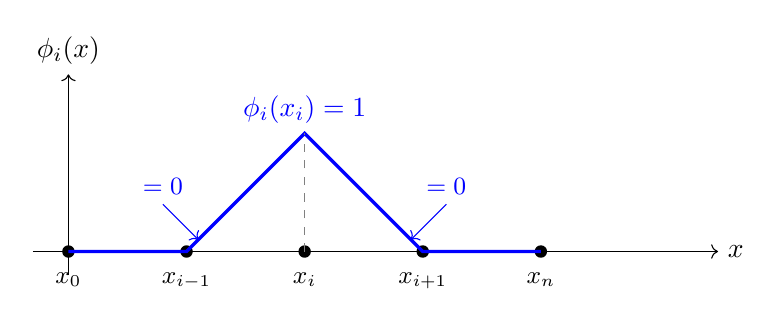
\begin{tikzpicture}[scale=1.5]
    % 坐标轴
    \draw[->] (-0.3,0) -- (5.5,0) node[right] {$x$};
    \draw[->] (0,-0.2) -- (0,1.5) node[above] {$\phi_i(x)$};
    
    % 网格节点
    \foreach \x/\lab in {0/$x_0$, 1/$x_{i-1}$, 2/$x_i$, 3/$x_{i+1}$, 4/$x_n$} {
        \fill (\x,0) circle (1.5pt);
        \node[below] at (\x,-0.1) {\small \lab};
    }
    
    % 形函数 φ_i
    \draw[very thick, blue] (0,0) -- (1,0) -- (2,1) -- (3,0) -- (4,0);
    
    % 标注
    \node[blue, above] at (2,1) {$\phi_i(x_i) = 1$};
    \draw[blue, <-] (1.1,0.1) -- (0.8,0.4) node[above] {\small $= 0$};
    \draw[blue, <-] (2.9,0.1) -- (3.2,0.4) node[above] {\small $= 0$};
    
    % 帐篷形状说明
    \draw[dashed, gray] (2,0) -- (2,1);
\end{tikzpicture}
\caption{帐篷函数 $\phi_i(x)$：在节点 $x_i$ 处等于 1，在相邻节点处等于 0，中间线性过渡}
\end{figure}

\paragraph{形函数的关键性质}

\begin{equation}
\phi_i(x_j) = \delta_{ij} = \begin{cases} 1, & i = j \\ 0, & i \neq j \end{cases}
\end{equation}

这个性质保证了：\textbf{系数 $U_i$ 恰好等于节点 $x_i$ 处的近似解值}！

验证：
\[
u_h(x_i) = \sum_j U_j \phi_j(x_i) = \sum_j U_j \delta_{ji} = U_i
\]

\subsection{从弱形式到线性方程组}

现在把近似解 $u_h = \sum_j U_j \phi_j$ 代入弱形式。

测试函数也用形函数：取 $v = \phi_i$（$i = 1, 2, \ldots, n$）

\paragraph{代入弱形式}

\[
\int_0^1 u_h' \cdot \phi_i' \, dx = \int_0^1 f \cdot \phi_i \, dx
\]

左边：
\[
\int_0^1 \left(\sum_j U_j \phi_j'\right) \phi_i' \, dx = \sum_j U_j \underbrace{\int_0^1 \phi_j' \phi_i' \, dx}_{K_{ij}}
\]

右边：
\[
\underbrace{\int_0^1 f \phi_i \, dx}_{F_i}
\]

于是得到：

\begin{keyformula}[title=有限元线性方程组]
\begin{equation}
\boxed{KU = F}
\end{equation}

其中：
\begin{itemize}
    \item $K_{ij} = \int_0^1 \phi_i'(x) \phi_j'(x) \, dx$ 是\textbf{刚度矩阵}的元素
    \item $F_i = \int_0^1 f(x) \phi_i(x) \, dx$ 是\textbf{载荷向量}的元素
    \item $U = (U_1, U_2, \ldots, U_n)^\top$ 是待求的\textbf{节点值向量}
\end{itemize}
\end{keyformula}

这就是有限元的核心方程！一个无限维的变分问题，变成了一个 $n \times n$ 的线性方程组。

% ------------------------------------------------------------------------------------
\section{刚度矩阵的计算}

\subsection{为什么叫"刚度矩阵"？}

"刚度"这个名字来自弹性力学。在弹簧系统中，$F = kx$，$k$ 是刚度——力与位移的比值。

在有限元中，$KU = F$ 说的是：\textbf{节点力 = 刚度矩阵 $\times$ 节点位移}。

$K_{ij}$ 的物理意义：给节点 $j$ 一个单位位移，节点 $i$ 受到多大的力？

\subsection{刚度矩阵的结构}

让我们计算刚度矩阵的元素 $K_{ij} = \int_0^1 \phi_i' \phi_j' dx$。

\paragraph{关键观察}

帐篷函数 $\phi_i$ 只在 $[x_{i-1}, x_{i+1}]$ 区间内非零（\textbf{局部支撑}）。

因此：
\begin{itemize}
    \item 如果 $|i - j| > 1$（节点不相邻），$\phi_i$ 和 $\phi_j$ 的支撑不重叠 $\Rightarrow$ $K_{ij} = 0$
    \item 只有 $|i - j| \leq 1$（相邻或相同节点）时，$K_{ij} \neq 0$
\end{itemize}

这导致刚度矩阵是\textbf{稀疏的三对角矩阵}！

\begin{figure}[h]
\centering
\begin{tikzpicture}[scale=0.6]
    % 画一个 5x5 的矩阵
    \draw[gray] (0,0) grid (5,5);
    
    % 填充非零元素
    % 主对角线
    \foreach \i in {0,...,4} {
        \fill[blue!60] (\i,4-\i) rectangle ++(1,1);
    }
    % 上下对角线
    \foreach \i in {0,...,3} {
        \fill[blue!30] (\i+1,4-\i) rectangle ++(1,1);
        \fill[blue!30] (\i,3-\i) rectangle ++(1,1);
    }
    
    % 标注
    \node at (2.5,-1) {三对角矩阵};
    \node[right] at (5.5,4.5) {\small $K_{11}$};
    \node[right] at (5.5,3.5) {\small $K_{22}$};
    \draw[->] (5.3,2.5) -- (4.2,2.5);
    \node[right] at (5.5,2.5) {\small 对角线};
\end{tikzpicture}
\caption{一维有限元的刚度矩阵是三对角的：只有相邻节点之间有耦合}
\end{figure}

\subsection{具体计算刚度矩阵元素}

设网格是均匀的，步长为 $h = \frac{1}{N}$，节点为 $x_k = kh$（$k = 0, 1, \ldots, N$）。

\paragraph{情况1：对角线元素 $K_{ii}$（$i$ 和自己的耦合）}

$\phi_i$ 在 $[x_{i-1}, x_i]$ 上斜率为 $+\frac{1}{h}$，在 $[x_i, x_{i+1}]$ 上斜率为 $-\frac{1}{h}$。

\begin{figure}[h]
\centering
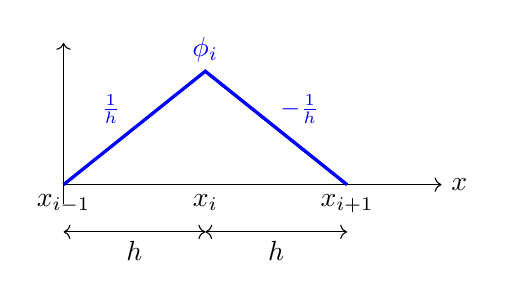
\begin{tikzpicture}[scale=1.2]
    \draw[->] (0,0) -- (4,0) node[right] {$x$};
    \draw[->] (0,-0.2) -- (0,1.5);
    
    % 形函数
    \draw[very thick, blue] (0,0) -- (1.5,1.2) -- (3,0);
    \node[blue, above] at (1.5,1.2) {$\phi_i$};
    
    % 斜率标注
    \node[blue] at (0.5,0.8) {\small $\frac{1}{h}$};
    \node[blue] at (2.5,0.8) {\small $-\frac{1}{h}$};
    
    % 节点
    \node[below] at (0,0) {$x_{i-1}$};
    \node[below] at (1.5,0) {$x_i$};
    \node[below] at (3,0) {$x_{i+1}$};
    
    % 区间标注
    \draw[<->] (0,-0.5) -- (1.5,-0.5) node[midway, below] {$h$};
    \draw[<->] (1.5,-0.5) -- (3,-0.5) node[midway, below] {$h$};
\end{tikzpicture}
\end{figure}

\begin{align}
K_{ii} &= \int_{x_{i-1}}^{x_{i+1}} (\phi_i')^2 \, dx \\
&= \int_{x_{i-1}}^{x_i} \left(\frac{1}{h}\right)^2 dx + \int_{x_i}^{x_{i+1}} \left(-\frac{1}{h}\right)^2 dx \\
&= \frac{1}{h^2} \cdot h + \frac{1}{h^2} \cdot h = \frac{2}{h}
\end{align}

\paragraph{情况2：相邻元素 $K_{i,i+1}$（相邻节点的耦合）}

$\phi_i$ 和 $\phi_{i+1}$ 只在 $[x_i, x_{i+1}]$ 上同时非零。

\begin{figure}[h]
\centering
\begin{tikzpicture}[scale=1.8]
    % 坐标轴
    \draw[->] (-0.3,0) -- (4.5,0) node[right] {$x$};
    \draw[->] (0,-0.2) -- (0,1.5) node[above] {};
    
    % 网格节点
    \foreach \x/\lab in {0/$x_{i-1}$, 1.5/$x_i$, 3/$x_{i+1}$, 4.5/$x_{i+2}$} {
        \fill (\x,0) circle (1.5pt);
    }
    \node[below] at (0,-0.1) {\small $x_{i-1}$};
    \node[below] at (1.5,-0.1) {\small $x_i$};
    \node[below] at (3,-0.1) {\small $x_{i+1}$};
    \node[below] at (4.2,-0.1) {\small $x_{i+2}$};
    
    % 形函数 φ_i (蓝色)
    \draw[very thick, blue] (0,0) -- (1.5,1.2) -- (3,0);
    \node[blue, above left] at (1.5,1.2) {$\phi_i$};
    
    % 形函数 φ_{i+1} (红色)
    \draw[very thick, red] (1.5,0) -- (3,1.2) -- (4.2,0);
    \node[red, above right] at (3,1.2) {$\phi_{i+1}$};
    
    % 重叠区域高亮
    \fill[purple, opacity=0.15] (1.5,0) -- (3,0) -- (3,1.2) -- (1.5,1.2) -- cycle;
    \fill[purple, opacity=0.15] (1.5,0) -- (1.5,1.2) -- (3,0) -- cycle;
    
    % 实际重叠的三角形区域（两个函数都非零的地方）
    \fill[green, opacity=0.2] (1.5,0) -- (2.25,0.6) -- (3,0) -- cycle;
    
    % 斜率标注
    \draw[blue, thick, ->] (2,0.4) -- (2.4,0.08);
    \node[blue] at (2.5,0.5) {\small $\phi_i' = -\dfrac{1}{h}$};
    
    \draw[red, thick, ->] (2.2,0.25) -- (2.6,0.57);
    \node[red] at (1.8,0.9) {\small $\phi_{i+1}' = +\dfrac{1}{h}$};
    
    % 区间标注
    \draw[<->, thick, purple] (1.5,-0.4) -- (3,-0.4);
    \node[purple, below] at (2.25,-0.4) {\small 重叠区间 $[x_i, x_{i+1}]$};
    
    % h 标注
    \draw[<->] (1.5,-0.7) -- (3,-0.7);
    \node at (2.25,-0.9) {\small $h$};
\end{tikzpicture}
\caption{相邻形函数 $\phi_i$ 和 $\phi_{i+1}$ 在区间 $[x_i, x_{i+1}]$ 上重叠。在此区间内，$\phi_i$ 下降（斜率 $-1/h$），$\phi_{i+1}$ 上升（斜率 $+1/h$），导致 $K_{i,i+1} < 0$。}
\end{figure}

在重叠区间 $[x_i, x_{i+1}]$ 上：
\begin{itemize}
    \item $\phi_i$ 从 1 下降到 0，斜率 $\phi_i' = -\dfrac{1}{h}$
    \item $\phi_{i+1}$ 从 0 上升到 1，斜率 $\phi_{i+1}' = +\dfrac{1}{h}$
\end{itemize}

\begin{align}
K_{i,i+1} &= \int_{x_i}^{x_{i+1}} \phi_i' \cdot \phi_{i+1}' \, dx \\
&= \int_{x_i}^{x_{i+1}} \left(-\frac{1}{h}\right) \cdot \left(+\frac{1}{h}\right) dx \\
&= -\frac{1}{h^2} \cdot h = \boxed{-\frac{1}{h}}
\end{align}

\begin{physicalmeaning}
$K_{i,i+1} < 0$ 的物理意义：相邻节点之间是\textbf{负耦合}。

用弹簧网络的比喻：节点 $i$ 和 $i+1$ 之间连着一根弹簧。当节点 $i$ 向上移动时，弹簧会把节点 $i+1$ 也往上拉——这就是负刚度系数的来源。

对角线元素 $K_{ii} = \frac{2}{h} > 0$（正刚度），非对角线元素 $K_{i,i+1} = -\frac{1}{h} < 0$（负耦合），这种结构保证了刚度矩阵的正定性。
\end{physicalmeaning}

\paragraph{情况3：不相邻元素 $K_{ij}$（$|i-j| > 1$）}

$\phi_i$ 和 $\phi_j$ 的支撑不重叠，所以：
\[
K_{ij} = \int_0^1 \phi_i' \phi_j' dx = 0
\]

\subsection{刚度矩阵的完整形式}

综合以上，对于均匀网格，内部节点（$i = 1, 2, \ldots, N-1$）的刚度矩阵是：

\begin{equation}
K = \frac{1}{h}
\begin{pmatrix}
2 & -1 & 0 & \cdots & 0 \\
-1 & 2 & -1 & \cdots & 0 \\
0 & -1 & 2 & \cdots & 0 \\
\vdots & & \ddots & \ddots & \vdots \\
0 & 0 & \cdots & -1 & 2
\end{pmatrix}
\end{equation}

\begin{insightbox}
\textbf{惊人的巧合}：对于均匀网格，有限元得到的矩阵 $\frac{1}{h}[-1, 2, -1]$ 与\textbf{二阶中心差分}完全相同！

但有限元的优势在于：
\begin{itemize}
    \item 可以处理非均匀网格
    \item 可以处理复杂几何（二维、三维）
    \item 有坚实的数学理论保证收敛
\end{itemize}
\end{insightbox}

% ------------------------------------------------------------------------------------
\section{完整例题：手算有限元}

让我们完整地手算一个例子，加深理解。

\subsection{问题设定}

求解：
\[
-u''(x) = 1, \quad x \in (0, 1), \quad u(0) = u(1) = 0
\]

使用 4 个单元（5 个节点），步长 $h = 0.25$。
\begin{figure}[h]
\centering
\begin{tikzpicture}[scale=1.2]
    % ===== 上半部分：各个加权形函数 =====
    \node[anchor=south] at (2,4.8) {\textbf{各个加权形函数}};
    
    % 坐标轴（上）
    \draw[->] (-0.3,3) -- (4.5,3) node[right] {\small $x$};
    \draw[->] (0,2.8) -- (0,4.7);
    
    % 节点位置
    \foreach \i in {0,1,2,3,4} {
        \fill (\i,3) circle (1.5pt);
    }
    
    % U_1 φ_1 (蓝色) - 高度 0.09375 × 10 = 0.9375 (放大显示)
    \draw[very thick, blue] (0,3) -- (1,3.75) -- (2,3);
    \node[blue, right] at (1.1,3.85) {\small $U_1\phi_1$};
    
    % U_2 φ_2 (红色) - 高度 0.125 × 10 = 1.25
    \draw[very thick, red] (1,3) -- (2,4) -- (3,3);
    \node[red, above] at (2,4.05) {\small $U_2\phi_2$};
    
    % U_3 φ_3 (green) - 高度 0.09375 × 10 = 0.9375
    \draw[very thick, green!60!black] (2,3) -- (3,3.75) -- (4,3);
    \node[green!60!black, left] at (2.9,3.85) {\small $U_3\phi_3$};
    
    % 节点值标注
    \node[blue, below] at (1,2.9) {\scriptsize $U_1$};
    \node[red, below] at (2,2.9) {\scriptsize $U_2$};
    \node[green!60!black, below] at (3,2.9) {\scriptsize $U_3$};
    
    % ===== 加号 =====
    \node at (2,2.3) {\Large $\Downarrow$ \normalsize 叠加};
    
    % ===== 下半部分：叠加结果 =====
    \node[anchor=south] at (2,1.3) {\textbf{近似解 $u_h(x) = \sum_{j=1}^{3} U_j \phi_j(x)$}};
    
    % 坐标轴（下）
    \draw[->] (-0.3,0) -- (4.5,0) node[right] {\small $x$};
    \draw[->] (0,-0.2) -- (0,1.3);
    
    % 节点
    \foreach \i in {0,1,2,3,4} {
        \fill (\i,0) circle (1.5pt);
    }
    \node[below] at (0,-0.1) {\scriptsize $0$};
    \node[below] at (4,-0.1) {\scriptsize $1$};
    
    % 叠加后的分段线性函数 (紫色粗线)
    \draw[very thick, purple] (0,0) -- (1,0.75) -- (2,1) -- (3,0.75) -- (4,0);
    
    % 节点值标注
    \fill[purple] (1,0.75) circle (2pt);
    \fill[purple] (2,1) circle (2pt);
    \fill[purple] (3,0.75) circle (2pt);
    \node[purple, above left] at (1,0.75) {\small $U_1$};
    \node[purple, above] at (2,1.05) {\small $U_2$};
    \node[purple, above right] at (3,0.75) {\small $U_3$};
    
    % 精确解（虚线）
    \draw[dashed, gray, thick, domain=0:4, samples=50] plot (\x, {(\x/4)*(1-\x/4)*4});
    \node[gray, right] at (4.2,0.5) {\small 精确解};
    
    % 边界条件
    \fill[blue] (0,0) circle (2pt);
    \fill[blue] (4,0) circle (2pt);
    \node[blue, above left] at (0,0.1) {\scriptsize $U_0=0$};
    \node[blue, above right] at (4,0.1) {\scriptsize $U_4=0$};
\end{tikzpicture}
\caption{有限元近似解的构造：$u_h(x) = U_1\phi_1(x) + U_2\phi_2(x) + U_3\phi_3(x)$。每个形函数 $\phi_j$ 在节点 $j$ 处取值为 1，乘以节点值 $U_j$ 后叠加得到分段线性的近似解。灰色虚线为精确解 $u(x) = \frac{x(1-x)}{2}$。}
\end{figure}

\begin{insightbox}{形函数的"插值"本质}
形函数的关键性质是 $\phi_i(x_j) = \delta_{ij}$（在自己的节点上等于1，在其他节点上等于0）。

这意味着：
\[
u_h(x_j) = \sum_{k=1}^{n} U_k \phi_k(x_j) = \sum_{k=1}^{n} U_k \delta_{kj} = U_j
\]

即：\textbf{近似解在节点处的值恰好等于我们要求的未知量 $U_j$}！

形函数的作用就是在节点之间进行\textbf{线性插值}，把离散的节点值"连接"成连续函数。
\end{insightbox}

\subsection{第一步：组装刚度矩阵}

对于内部 3 个自由度，刚度矩阵是 $3 \times 3$：

\[
K = \frac{1}{h}
\begin{pmatrix}
2 & -1 & 0 \\
-1 & 2 & -1 \\
0 & -1 & 2
\end{pmatrix}
= \frac{1}{0.25}
\begin{pmatrix}
2 & -1 & 0 \\
-1 & 2 & -1 \\
0 & -1 & 2
\end{pmatrix}
=
\begin{pmatrix}
8 & -4 & 0 \\
-4 & 8 & -4 \\
0 & -4 & 8
\end{pmatrix}
\]

\subsection{第二步：计算载荷向量}

对于 $f(x) = 1$，载荷向量的第 $i$ 个分量为：
\[
F_i = \int_0^1 1 \cdot \phi_i(x) \, dx
\]

$\phi_i$ 是一个"帐篷"，底边宽 $2h$，高度为 1，面积为：
\[
F_i = \frac{1}{2} \times 2h \times 1 = h = 0.25
\]

（边界节点的形函数只有半个帐篷，但它们对应 $U_0 = U_4 = 0$，不参与方程。）

载荷向量：
\[
F = \begin{pmatrix} 0.25 \\ 0.25 \\ 0.25 \end{pmatrix}
\]

\subsection{第三步：求解线性方程组}

现在求解：
\[
\begin{pmatrix}
8 & -4 & 0 \\
-4 & 8 & -4 \\
0 & -4 & 8
\end{pmatrix}
\begin{pmatrix} U_1 \\ U_2 \\ U_3 \end{pmatrix}
=
\begin{pmatrix} 0.25 \\ 0.25 \\ 0.25 \end{pmatrix}
\]

\paragraph{用高斯消元法求解}

第一个方程：$8U_1 - 4U_2 = 0.25$

第二个方程加上第一个方程的 $\frac{1}{2}$ 倍：
\[
(-4 + 4)U_1 + (8 - 2)U_2 - 4U_3 = 0.25 + 0.125 \quad \Rightarrow \quad 6U_2 - 4U_3 = 0.375
\]

第三个方程加上新的第二个方程的 $\frac{2}{3}$ 倍：
\[
(8 - \frac{8}{3})U_3 = 0.25 + 0.25 \quad \Rightarrow \quad \frac{16}{3}U_3 = 0.5 \quad \Rightarrow \quad U_3 = 0.09375
\]

回代：
\[
U_2 = \frac{0.375 + 4 \times 0.09375}{6} = \frac{0.75}{6} = 0.125
\]
\[
U_1 = \frac{0.25 + 4 \times 0.125}{8} = \frac{0.75}{8} = 0.09375
\]

\subsection{第四步：检验结果}

有限元解：
\[
U_1 = U_3 = 0.09375, \quad U_2 = 0.125
\]

精确解 $u(x) = \frac{x(1-x)}{2}$ 在节点处的值：
\[
u(0.25) = \frac{0.25 \times 0.75}{2} = 0.09375
\]
\[
u(0.5) = \frac{0.5 \times 0.5}{2} = 0.125
\]
\[
u(0.75) = \frac{0.75 \times 0.25}{2} = 0.09375
\]

\textbf{有限元解在节点处恰好等于精确解！}

\begin{figure}[h]
\centering
\begin{tikzpicture}[x=6cm, y=15cm]
    % 坐标轴
    \draw[->] (-0.05,0) -- (1.15,0) node[right] {$x$};
    \draw[->] (0,-0.01) -- (0,0.15) node[above] {$u(x)$};
    
    % 刻度
    \foreach \x in {0, 0.25, 0.5, 0.75, 1} {
        \draw (\x,0) -- (\x,-0.005);
        \node[below] at (\x,-0.005) {\scriptsize $\x$};
    }
    \foreach \y in {0, 0.05, 0.1} {
        \draw (0,\y) -- (-0.02,\y);
        \node[left] at (-0.02,\y) {\scriptsize $\y$};
    }
    
    % 精确解
    \draw[thick, gray, dashed, domain=0:1, samples=50] plot (\x, {0.5*\x*(1-\x)});
    \node[gray] at (0.85,0.11) {\small 精确解};
    
    % 有限元解
    \draw[very thick, blue] (0,0) -- (0.25,0.09375) -- (0.5,0.125) -- (0.75,0.09375) -- (1,0);
    \node[blue] at (0.15,0.06) {\small $u_h(x)$};
    
    % 节点
    \fill[red] (0.25,0.09375) circle (2pt);
    \fill[red] (0.5,0.125) circle (2pt);
    \fill[red] (0.75,0.09375) circle (2pt);
\end{tikzpicture}
\caption{有限元解（蓝色折线）与精确解（灰色虚线）的对比}
\end{figure}

\begin{insightbox}
\textbf{超收敛现象}：对于一维问题和线性形函数，有限元解在节点处恰好等于精确解！

这是一维问题的特殊性质。在二维、三维问题中，有限元解在节点处通常只是近似值，但仍然是"最优"的（在能量范数意义下）。
\end{insightbox}

% ------------------------------------------------------------------------------------
\section{单元组装：从局部到整体}

在实际计算中，我们不直接计算整体刚度矩阵。而是：
\begin{enumerate}
    \item 在每个小\textbf{单元}上计算\textbf{单元刚度矩阵}
    \item 把所有单元刚度矩阵\textbf{组装}成整体刚度矩阵
\end{enumerate}

这种"分而治之"的策略使有限元方法非常灵活——可以处理不规则网格、不同类型的单元混合等。

\subsection{单元刚度矩阵}

对于一维线性单元（两个节点），单元刚度矩阵是 $2 \times 2$ 的：

\begin{keyformula}[title=一维线性单元刚度矩阵]
\begin{equation}
K^e = \frac{1}{h}
\begin{pmatrix}
1 & -1 \\
-1 & 1
\end{pmatrix}
\end{equation}

行和列分别对应单元的左节点和右节点。
\end{keyformula}

\paragraph{推导}

设单元长度为 $h$，两端节点为 $x_L$ 和 $x_R$。

单元内的两个形函数：
\[
N_L(x) = \frac{x_R - x}{h}, \quad N_R(x) = \frac{x - x_L}{h}
\]

它们的导数：
\[
N_L' = -\frac{1}{h}, \quad N_R' = \frac{1}{h}
\]

单元刚度矩阵的元素：
\[
K^e_{LL} = \int_{x_L}^{x_R} (N_L')^2 dx = \frac{1}{h^2} \cdot h = \frac{1}{h}
\]
\[
K^e_{LR} = \int_{x_L}^{x_R} N_L' N_R' dx = -\frac{1}{h^2} \cdot h = -\frac{1}{h}
\]
\[
K^e_{RR} = \int_{x_L}^{x_R} (N_R')^2 dx = \frac{1}{h^2} \cdot h = \frac{1}{h}
\]

\subsection{组装过程}

组装的规则很简单：把每个单元刚度矩阵"放入"整体矩阵的对应位置，重叠处累加。

\begin{figure}[h]
\centering
\begin{tikzpicture}[scale=0.6]
    % 单元1矩阵（用数学矩阵表示，不用tikz框）
    \node[anchor=east] at (-2,6) {\small 单元1 (节点0-1):};
    \node at (0,6) {$\begin{pmatrix} \frac{1}{h} & -\frac{1}{h} \\[3pt] -\frac{1}{h} & \frac{1}{h} \end{pmatrix}$};

    % 箭头指向蓝色区域
    \draw[->, thick, blue!70] (1.8,6) -- (4.2,4.5);

    % 单元2矩阵
    \node[anchor=east] at (-2,2) {\small 单元2 (节点1-2):};
    \node at (0,2) {$\begin{pmatrix} \frac{1}{h} & -\frac{1}{h} \\[3pt] -\frac{1}{h} & \frac{1}{h} \end{pmatrix}$};

    % 箭头指向橙色区域
    \draw[->, thick, orange!80] (1.8,2) -- (5.2,2.5);

    % 整体矩阵框架
    \draw[thick] (4,0) grid (9,5);

    % 填充蓝色区域（单元1贡献：节点0,1）
    \fill[blue!25] (4,4) rectangle (5,5);
    \fill[blue!25] (5,4) rectangle (6,5);
    \fill[blue!25] (4,3) rectangle (5,4);
    \fill[blue!25] (5,3) rectangle (6,4);

    % 填充橙色区域（单元2贡献：节点1,2）
    \fill[orange!25] (5,3) rectangle (6,4);
    \fill[orange!25] (6,3) rectangle (7,4);
    \fill[orange!25] (5,2) rectangle (6,3);
    \fill[orange!25] (6,2) rectangle (7,3);

    % 重叠处（节点1的对角元）用红色标出
    \fill[red!40] (5,3) rectangle (6,4);
    \node[font=\footnotesize] at (5.5,3.5) {$\frac{2}{h}$};

    % 列标签（在矩阵上方）
    \foreach \i in {0,...,4} {
        \node[above, font=\scriptsize] at (4.5+\i,5.1) {\i};
    }
    % 行标签（在矩阵左侧）
    \foreach \i in {0,...,4} {
        \node[left, font=\scriptsize] at (3.9,4.5-\i) {\i};
    }

    % 整体矩阵标题
    \node[above] at (6.5,5.5) {\small 整体刚度矩阵 $K$};

    % 说明文字
    \node at (6.5,-0.8) {\small 重叠处累加：$\frac{1}{h} + \frac{1}{h} = \frac{2}{h}$};
\end{tikzpicture}
\caption{组装过程示意：单元矩阵放入整体矩阵对应位置，重叠处累加}
\end{figure}

\begin{physicalmeaning}
\textbf{组装的物理意义}：

\begin{itemize}
    \item 对角线元素 $K_{ii}$ 累加了所有与节点 $i$ 相连的单元贡献——节点的"总刚度"
    \item 非对角线元素 $K_{ij}$ 只来自同时包含 $i$ 和 $j$ 的单元——节点间的"耦合"
\end{itemize}

就像一个弹簧网络：每个节点的总刚度是连接它的所有弹簧刚度之和。
\end{physicalmeaning}

% ------------------------------------------------------------------------------------
\section{边界条件处理}

\subsection{Dirichlet 边界条件（固定值）}

我们的例子中，$u(0) = u(1) = 0$ 是 Dirichlet 边界条件——边界上的值是固定的。

\paragraph{处理方法1：直接消去}

既然 $U_0 = U_4 = 0$ 是已知的，就从方程组中删去这两个未知量，只求解内部节点。

这就是我们上面手算例子用的方法。

\paragraph{处理方法2：大数法（罚函数）}

把对角线元素改成一个很大的数，对应的载荷也相应修改：

\[
K_{00} \leftarrow 10^{20}, \quad F_0 \leftarrow 10^{20} \times g_0
\]

其中 $g_0$ 是边界值。这样方程 $10^{20} U_0 = 10^{20} g_0$ 就强制 $U_0 \approx g_0$。

\textbf{优点}：不改变矩阵结构，易于编程

\textbf{缺点}：矩阵条件数变差

\subsection{Neumann 边界条件（给定导数）}

如果边界条件是 $u'(1) = q$（给定热流），这是 Neumann 边界条件。

Neumann 条件在弱形式中\textbf{自然满足}——它会贡献到载荷向量：
\[
F_n \leftarrow F_n + q
\]

\subsection{拉格朗日乘子法}

和第1章一样，我们也可以用拉格朗日乘子处理边界条件！

把边界条件 $u(0) = g$ 看作约束，引入乘子 $\lambda$：
\[
\mathcal{L}[u, \lambda] = J[u] + \lambda(u(0) - g)
\]

这导出一个\textbf{鞍点问题}：
\[
\begin{pmatrix}
K & B^\top \\
B & 0
\end{pmatrix}
\begin{pmatrix}
U \\
\lambda
\end{pmatrix}
=
\begin{pmatrix}
F \\
g
\end{pmatrix}
\]

\begin{physicalmeaning}
$\lambda$ 的物理意义是边界处的\textbf{法向通量}：
\begin{itemize}
    \item 热传导：$\lambda$ = 热流密度（W/m²）
    \item 弹性力学：$\lambda$ = 边界反力（N）
\end{itemize}

这与第5章力学中的约束力完全对应——边界条件本质上也是约束！
\end{physicalmeaning}

% ------------------------------------------------------------------------------------
\section{误差分析与收敛性}

\subsection{误差的来源}

有限元解 $u_h$ 与精确解 $u$ 之间有误差。误差来自哪里？

\begin{itemize}
    \item \textbf{离散化误差}：用有限维空间逼近无限维空间
    \item \textbf{插值误差}：用分片多项式逼近光滑函数
\end{itemize}

\subsection{误差估计}

对于线性形函数，误差有如下估计：

\begin{keytheorem}[title=有限元误差估计]
设 $u$ 是精确解，$u_h$ 是线性有限元解，$h$ 是网格步长。则：

\textbf{能量范数误差}：
\[
\|u' - u_h'\|_{L^2} \leq Ch \|u''\|_{L^2}
\]

\textbf{$L^2$ 范数误差}：
\[
\|u - u_h\|_{L^2} \leq Ch^2 \|u''\|_{L^2}
\]

其中 $C$ 是与 $h$ 无关的常数。
\end{keytheorem}

\paragraph{含义}

\begin{itemize}
    \item 网格加密一倍（$h \to h/2$），导数误差减半，函数值误差减到 $\frac{1}{4}$
    \item 线性元的收敛阶是 $O(h)$（能量范数）或 $O(h^2)$（$L^2$ 范数）
    \item 用更高阶的多项式（如二次元、三次元），可以获得更高的收敛阶
\end{itemize}

\subsection{数值验证}

让我们用不同的网格密度求解 $-u'' = 1$，验证收敛性：

\begin{center}
\begin{tabular}{c|c|c|c}
\toprule
单元数 $N$ & 步长 $h$ & 最大误差 & 误差比 \\
\midrule
4 & 0.25 & $7.8 \times 10^{-3}$ & -- \\
8 & 0.125 & $2.0 \times 10^{-3}$ & 3.9 \\
16 & 0.0625 & $4.9 \times 10^{-4}$ & 4.1 \\
32 & 0.03125 & $1.2 \times 10^{-4}$ & 4.1 \\
\bottomrule
\end{tabular}
\end{center}

每次加密一倍，误差减少到约 $\frac{1}{4}$——符合 $O(h^2)$ 的理论预测！

% ------------------------------------------------------------------------------------
\section{二维问题简介}

\subsection{从一维到二维}

一维的思想可以自然推广到二维。

\textbf{二维 Poisson 方程}：
\[
-\nabla^2 u = -\left(\frac{\partial^2 u}{\partial x^2} + \frac{\partial^2 u}{\partial y^2}\right) = f \quad \text{in } \Omega
\]

\textbf{弱形式}：
\[
\int_\Omega \nabla u \cdot \nabla v \, dA = \int_\Omega fv \, dA
\]

\textbf{离散化}：把区域 $\Omega$ 剖分成三角形或四边形单元。

\begin{figure}[h]
\centering
\begin{tikzpicture}[scale=0.8]
    % 区域
    \draw[thick] (0,0) -- (4,0) -- (4,3) -- (0,3) -- cycle;
    
    % 三角形网格
    \foreach \x in {0,1,...,4} {
        \foreach \y in {0,1,2,3} {
            \fill (\x,\y) circle (1.5pt);
        }
    }
    
    % 画一些三角形
    \draw[gray] (0,0) -- (1,1) -- (0,1) -- cycle;
    \draw[gray] (0,0) -- (1,0) -- (1,1) -- cycle;
    \draw[gray] (1,0) -- (2,1) -- (1,1) -- cycle;
    \draw[gray] (1,0) -- (2,0) -- (2,1) -- cycle;
    \draw[gray] (2,0) -- (3,1) -- (2,1) -- cycle;
    \draw[gray] (2,0) -- (3,0) -- (3,1) -- cycle;
    \draw[gray] (3,0) -- (4,1) -- (3,1) -- cycle;
    \draw[gray] (3,0) -- (4,0) -- (4,1) -- cycle;
    
    \draw[gray] (0,1) -- (1,2) -- (0,2) -- cycle;
    \draw[gray] (0,1) -- (1,1) -- (1,2) -- cycle;
    \draw[gray] (1,1) -- (2,2) -- (1,2) -- cycle;
    \draw[gray] (1,1) -- (2,1) -- (2,2) -- cycle;
    \draw[gray] (2,1) -- (3,2) -- (2,2) -- cycle;
    \draw[gray] (2,1) -- (3,1) -- (3,2) -- cycle;
    \draw[gray] (3,1) -- (4,2) -- (3,2) -- cycle;
    \draw[gray] (3,1) -- (4,1) -- (4,2) -- cycle;
    
    \draw[gray] (0,2) -- (1,3) -- (0,3) -- cycle;
    \draw[gray] (0,2) -- (1,2) -- (1,3) -- cycle;
    \draw[gray] (1,2) -- (2,3) -- (1,3) -- cycle;
    \draw[gray] (1,2) -- (2,2) -- (2,3) -- cycle;
    \draw[gray] (2,2) -- (3,3) -- (2,3) -- cycle;
    \draw[gray] (2,2) -- (3,2) -- (3,3) -- cycle;
    \draw[gray] (3,2) -- (4,3) -- (3,3) -- cycle;
    \draw[gray] (3,2) -- (4,2) -- (4,3) -- cycle;
    
    % 标注
    \node at (2,-0.8) {三角形网格剖分};
\end{tikzpicture}
\caption{二维有限元：区域被剖分成三角形单元}
\end{figure}

\subsection{三角形单元}

最简单的二维单元是线性三角形单元。每个三角形有 3 个节点，单元内的近似解是：
\[
u_h(x, y) = U_1 N_1(x,y) + U_2 N_2(x,y) + U_3 N_3(x,y)
\]

其中 $N_i$ 是线性形函数，满足 $N_i(x_j, y_j) = \delta_{ij}$。

\paragraph{单元刚度矩阵}

三角形单元的刚度矩阵是 $3 \times 3$：
\[
K^e_{ij} = \int_{\text{三角形}} \nabla N_i \cdot \nabla N_j \, dA
\]

由于 $N_i$ 是线性函数，$\nabla N_i$ 是常向量，积分很容易计算。

\subsection{刚度矩阵的稀疏性}

二维问题的刚度矩阵仍然是稀疏的——只有相邻节点之间有耦合。

但稀疏结构更复杂：不再是三对角，而是\textbf{带状稀疏}矩阵。

\begin{figure}[h]
\centering
\begin{tikzpicture}[scale=0.08]
    % 画一个稀疏矩阵的样子
    \draw[gray] (0,0) rectangle (50,50);
    
    % 用随机点表示非零元素
    \foreach \i in {0,...,49} {
        \fill[blue] (\i,49-\i) circle (1);
        \pgfmathsetmacro{\jone}{int(\i+1)}
        \pgfmathsetmacro{\jtwo}{int(\i+2)}
        \pgfmathsetmacro{\jthree}{int(\i+5)}
        \pgfmathsetmacro{\jfour}{int(\i+6)}
        \ifnum\i<49
            \fill[blue!50] (\jone,49-\i) circle (0.8);
            \fill[blue!50] (\i,49-\jone) circle (0.8);
        \fi
        \ifnum\i<48
            \fill[blue!30] (\jtwo,49-\i) circle (0.6);
            \fill[blue!30] (\i,49-\jtwo) circle (0.6);
        \fi
        \ifnum\i<45
            \fill[blue!20] (\jthree,49-\i) circle (0.5);
            \fill[blue!20] (\i,49-\jthree) circle (0.5);
        \fi
    }
    
    \node at (25,-8) {\small 二维有限元的稀疏刚度矩阵};
\end{tikzpicture}
\end{figure}

% ------------------------------------------------------------------------------------
% ------------------------------------------------------------------------------------
\section{殊途同归：有限差分与有限元}

在继续深入之前，让我们回答一个常见问题：有限差分法（FDM）和有限元法（FEM）有什么区别？

\subsection{一维情况：完全等价}

考虑一维问题 $-u'' = f$，用 $N$ 个等距节点离散化。

\begin{figure}[h]
\centering
\begin{tikzpicture}[scale=1.2]
    % 左边：FDM
    \node[font=\bfseries] at (-3, 2) {有限差分 (FDM)};
    \draw[->] (-5, 0) -- (-1, 0) node[right] {$x$};
    \foreach \i in {0,1,2,3,4} {
        \fill (-5+\i, 0) circle (2pt);
        \node[below] at (-5+\i, -0.2) {\small $x_\i$};
    }
    % Taylor展开示意
    \draw[blue, thick, ->] (-3, 0.3) -- (-4, 0.3);
    \draw[blue, thick, ->] (-3, 0.3) -- (-2, 0.3);
    \node[blue, above] at (-3, 0.4) {\small Taylor展开};
    
    % 右边：FEM
    \node[font=\bfseries] at (3, 2) {有限元 (FEM)};
    \draw[->] (1, 0) -- (5, 0) node[right] {$x$};
    \foreach \i in {0,1,2,3,4} {
        \fill (1+\i, 0) circle (2pt);
    }
    % 形函数示意
    \draw[red, thick] (1,0) -- (2,0.8) -- (3,0);
    \draw[red, thick] (2,0) -- (3,0.8) -- (4,0);
    \node[red, above] at (3, 0.9) {\small 形函数};
\end{tikzpicture}
\caption{有限差分 vs 有限元的离散化方式}
\end{figure}

\vspace{0.3cm}
\noindent
\begin{minipage}[t]{0.48\textwidth}
\textbf{有限差分的推导}

出发点：Taylor展开近似导数
\[
-u''(x_i) \approx -\frac{u_{i+1} - 2u_i + u_{i-1}}{h^2}
\]

离散方程（第 $i$ 行）：
\[
\frac{-u_{i-1} + 2u_i - u_{i+1}}{h^2} = f_i
\]

系数：$\left[ -\frac{1}{h^2}, \; \frac{2}{h^2}, \; -\frac{1}{h^2} \right]$
\end{minipage}
\hfill
\begin{minipage}[t]{0.48\textwidth}
\textbf{有限元的推导}

出发点：弱形式 + 线性形函数
\[
K_{ij} = \int \phi_i' \phi_j' dx
\]

刚度矩阵（第 $i$ 行）：
\[
\frac{1}{h} [-1, \quad 2, \quad -1]
\]

方程：$\frac{-U_{i-1} + 2U_i - U_{i+1}}{h} = hf_i$
\end{minipage}

\vspace{0.5cm}
把FEM方程两边除以 $h$：
\[
\frac{-U_{i-1} + 2U_i - U_{i+1}}{h^2} = f_i
\]

\begin{insightbox}
在一维均匀网格上，线性有限元和中心差分给出\textbf{完全相同}的方程！

这不是巧合——两种方法从不同角度逼近了同一个物理问题。
\end{insightbox}



\subsection{二维情况：分道扬镳}

当问题升级到二维，两种方法开始展现本质区别。

\textbf{任务}：在圆形区域 $\Omega$ 上求解 $-\Delta u = f$。

\begin{figure}[h]
\centering
\begin{tikzpicture}[scale=1.8]
    % 左边：FDM
    \begin{scope}[xshift=-3cm]
        \node[font=\bfseries] at (0.5, 1.3) {有限差分};
        % 规则网格
        \draw[step=0.2, gray!30, thin] (0,0) grid (1.1,1.1);
        % 真实圆边界
        \draw[thick, red] (0,1) arc (90:0:1);
        % 锯齿逼近
        \draw[blue, thick]
            (0,1) -- (0.2,1) -- (0.2,0.8) --
            (0.4,0.8) -- (0.4,0.6) --
            (0.6,0.6) -- (0.6,0.4) --
            (0.8,0.4) -- (0.8,0.2) --
            (1.0,0.2) -- (1.0,0);
        % 五点差分模板
        \fill[blue] (0.6,0.4) circle (1pt);
        \foreach \dx/\dy in {0.2/0, -0.2/0, 0/0.2, 0/-0.2}{
            \draw[->, thick, blue!60] (0.6,0.4) -- +(\dx,\dy);
        }
        \node[red, font=\scriptsize] at (0.5, 1.15) {真实边界};
        \node[blue, font=\scriptsize] at (0.2, 0.5) {锯齿};
    \end{scope}
    
    % 右边：FEM
    \begin{scope}[xshift=1.5cm]
        \node[font=\bfseries] at (0.5, 1.3) {有限元};
        % 真实圆边界
        \draw[thick, red] (0,1) arc (90:0:1);
        % 三角剖分
        \coordinate (O) at (0,0);
        \coordinate (B) at (0,1);
        \coordinate (C) at (0.5,0.866);
        \coordinate (D) at (0.866,0.5);
        \coordinate (E) at (1,0);
        \coordinate (b) at (0,0.5);
        \coordinate (c) at (0.25,0.433);
        \coordinate (d) at (0.433,0.25);
        \coordinate (e) at (0.5,0);
        
        \draw[blue] (O) -- (b) -- (c) -- cycle;
        \draw[blue] (O) -- (c) -- (d) -- cycle;
        \draw[blue] (O) -- (d) -- (e) -- cycle;
        \draw[blue] (b) -- (B) -- (C) -- (c) -- cycle;
        \draw[blue] (c) -- (C) -- (D) -- (d) -- cycle;
        \draw[blue] (d) -- (D) -- (E) -- (e) -- cycle;
        
        % 边界节点
        \foreach \P in {B,C,D,E} {
            \fill[red] (\P) circle (1.5pt);
        }
        \node[blue, font=\scriptsize] at (0.5, 0.5) {三角形};
        \node[red, font=\scriptsize] at (0.7, 1.0) {节点在边界上};
    \end{scope}
\end{tikzpicture}
\caption{二维圆形区域的离散化：FDM用锯齿逼近边界，FEM可以精确贴合。}
\end{figure}

\begin{center}
\renewcommand{\arraystretch}{1.4}
\begin{tabular}{l|p{5cm}|p{5cm}}
\toprule
& \textbf{有限差分} & \textbf{有限元} \\
\midrule
网格类型 & 结构化（规则方格） & 非结构化（任意三角形） \\
边界处理 & 锯齿逼近，精度损失 & 节点直接在边界上 \\
复杂几何 & 困难（需要特殊处理） & 自然（只需网格生成） \\
实现难度 & 简单（数组索引） & 复杂（邻接关系） \\
适用场景 & 规则区域（图像、芯片） & 复杂几何（飞机、骨骼） \\
\bottomrule
\end{tabular}
\end{center}

\begin{physicalmeaning}
\textbf{为什么FEM统治了工程计算？}

现实世界的几何很少是规则的：飞机机翼是流线型的，人体骨骼是弯曲的，汽车车身是复杂曲面。

有限元的三角形/四面体网格可以\textbf{贴合任意几何形状}，这是它在工程中广泛应用的根本原因。

代价是：需要维护复杂的网格数据结构和邻接关系。
\end{physicalmeaning}

% ------------------------------------------------------------------------------------
\section{连续性的秘密}

\subsection{为什么要求连续？}

在前面的推导中，我们默默假设了 $u_h(x)$ 是连续的。但为什么？

\begin{figure}[h]
\centering
\begin{tikzpicture}[scale=1.2]
    % 上半部分：连续函数
    \begin{scope}[yshift=2cm]
        \draw[->] (0,0) -- (4,0) node[right] {$x$};
        \draw[->] (0,0) -- (0,1.5);
        \draw[blue, very thick] (0.5, 0.3) -- (2, 1.2) -- (3.5, 0.8);
        \node[blue] at (2, 1.5) {连续折线};
        \node[blue, align=center] at (5, 0.8) {导数有限 \\ 能量有限 $\checkmark$};
    \end{scope}
    
    % 下半部分：不连续函数
    \begin{scope}
        \draw[->] (0,0) -- (4,0) node[right] {$x$};
        \draw[->] (0,0) -- (0,1.5);
        \draw[red, very thick] (0.5, 0.3) -- (2, 1.2);
        \draw[red, very thick] (2, 0.4) -- (3.5, 0.8);
        \draw[red, dashed] (2, 0.4) -- (2, 1.2);
        \node[red] at (2.3, 0.8) {Jump!};
        \node[red, align=center] at (5, 0.8) {导数 $= \infty$ \\ 能量 $= \infty$ $\times$};
    \end{scope}
\end{tikzpicture}
\caption{连续性与能量的关系}
\end{figure}

\textbf{数学解释}：我们的弱形式包含梯度项 $\int |\nabla u|^2 dx$（能量）。

如果 $u$ 在某点有跳跃（不连续）：
\begin{itemize}
    \item 导数 $u'$ 在该点变成 Dirac $\delta$ 函数（无穷大）
    \item 能量 $\int (u')^2 dx = \int \delta^2 dx = \infty$
\end{itemize}

物理上，无穷大的能量是不允许的。

\begin{keyformula}[title=$C^0$ 连续性]
我们要求有限元解空间 $V_h \subset C^0(\Omega)$，即：

\textbf{函数值连续，但导数可以不连续}

换句话说：$u_h$ 可以"折"，但不能"断"。
\end{keyformula}

\subsection{线性单元如何保证连续？}

一个关键问题：我们只要求\textbf{节点值}相等，怎么能保证整条公共边上都连续？

\begin{figure}[h]
\centering
\begin{tikzpicture}[scale=1.5]
    % 两个三角形共享边
    \coordinate (N1) at (0,1);
    \coordinate (N2) at (0,-1);
    \coordinate (N3) at (-1.5, 0);
    \coordinate (N4) at (1.5, 0);
    
    \draw[fill=blue!10] (N1) -- (N2) -- (N3) -- cycle;
    \draw[fill=orange!10] (N1) -- (N2) -- (N4) -- cycle;
    
    % 共享边
    \draw[ultra thick, red] (N1) -- (N2);
    
    % 节点标注
    \node[above] at (N1) {$U_1$};
    \node[below] at (N2) {$U_2$};
    \node[left] at (N3) {$U_3$};
    \node[right] at (N4) {$U_4$};
    
    \node[blue] at (-0.7, 0) {单元 A};
    \node[orange] at (0.7, 0) {单元 B};
    
    % 边上的点
    \fill[black] (0, 0.3) circle (1.5pt) node[right] {$P$};
\end{tikzpicture}
\caption{两个三角形共享边 1-2}
\end{figure}

\textbf{几何证明}：

\begin{enumerate}
    \item 在三角形 A 内部，$u_h$ 是一个\textbf{平面}（线性函数）
    
    \item 这个平面在边 1-2 上截出一条\textbf{直线}
    
    \item 这条直线由两个端点值 $U_1$ 和 $U_2$ \textbf{唯一确定}（两点定一线！）
    
    \item 同样，三角形 B 在边 1-2 上也截出一条直线，也由 $U_1$ 和 $U_2$ 确定
    
    \item 两条直线端点相同 $\Rightarrow$ 两条直线重合！
\end{enumerate}

\begin{insightbox}
\textbf{线性单元连续性的关键}：两点确定一条直线。

只要共享节点的值相同，整条公共边就自动连续——就像\textbf{合页(Hinge)}一样严丝合缝。

这就是为什么线性单元只需要在顶点处设置自由度。
\end{insightbox}

\textbf{高阶单元怎么办？}

如果是二次单元，边上的函数是抛物线。两点定不了抛物线！

解决方案：在边的中点增加一个节点，三点定抛物线。

\begin{figure}[h]
\centering
\begin{tikzpicture}[scale=1.2]
    % 线性单元
    \begin{scope}
        \node[font=\bfseries] at (1, 1.8) {线性单元};
        \draw[thick] (0,0) -- (2,0) -- (1,1.5) -- cycle;
        \fill[blue] (0,0) circle (3pt);
        \fill[blue] (2,0) circle (3pt);
        \fill[blue] (1,1.5) circle (3pt);
        \node[below] at (1, -0.3) {3个节点};
    \end{scope}
    
    % 二次单元
    \begin{scope}[xshift=5cm]
        \node[font=\bfseries] at (1, 1.8) {二次单元};
        \draw[thick] (0,0) -- (2,0) -- (1,1.5) -- cycle;
        % 顶点
        \fill[blue] (0,0) circle (3pt);
        \fill[blue] (2,0) circle (3pt);
        \fill[blue] (1,1.5) circle (3pt);
        % 边中点
        \fill[red] (1,0) circle (3pt);
        \fill[red] (1.5,0.75) circle (3pt);
        \fill[red] (0.5,0.75) circle (3pt);
        \node[below] at (1, -0.3) {6个节点};
    \end{scope}
\end{tikzpicture}
\caption{线性单元（3节点）vs 二次单元（6节点）}
\end{figure}

\subsection{一维二次单元详解}

为了理解高阶单元，让我们先看最简单的情况：一维二次单元。

\begin{figure}[h]
\centering
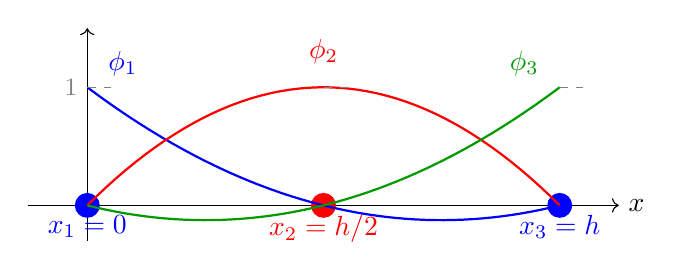
\begin{tikzpicture}[scale=1.5]
    % 坐标轴
    \draw[->] (-0.5, 0) -- (4.5, 0) node[right] {$x$};
    \draw[->] (0, -0.3) -- (0, 1.5);
    
    % 三个节点
    \fill[blue] (0, 0) circle (3pt) node[below] {$x_1 = 0$};
    \fill[red] (2, 0) circle (3pt) node[below] {$x_2 = h/2$};
    \fill[blue] (4, 0) circle (3pt) node[below] {$x_3 = h$};
    
    % 三个形函数
    % φ_1: 在x_1=1, 其他=0
    \draw[blue, thick, domain=0:4, samples=50] plot (\x, {((\x-2)*(\x-4))/((-2)*(-4))});
    \node[blue] at (0.3, 1.2) {$\phi_1$};
    
    % φ_2: 在x_2=1, 其他=0
    \draw[red, thick, domain=0:4, samples=50] plot (\x, {((\x-0)*(\x-4))/((2-0)*(2-4))});
    \node[red] at (2, 1.3) {$\phi_2$};
    
    % φ_3: 在x_3=1, 其他=0
    \draw[green!60!black, thick, domain=0:4, samples=50] plot (\x, {((\x-0)*(\x-2))/((4-0)*(4-2))});
    \node[green!60!black] at (3.7, 1.2) {$\phi_3$};
    
    % 高度标记
    \draw[dashed, gray] (0, 1) -- (0.2, 1);
    \node[left, gray] at (0, 1) {\small 1};
    \draw[dashed, gray] (2, 1) -- (2.2, 1);
    \draw[dashed, gray] (4, 1) -- (4.2, 1);
\end{tikzpicture}
\caption{一维二次单元的三个形函数：都是抛物线！}
\end{figure}

\textbf{二次形函数的公式}

用拉格朗日插值构造（三点定抛物线）：

\begin{align}
\phi_1(x) &= \frac{(x - x_2)(x - x_3)}{(x_1 - x_2)(x_1 - x_3)} = \frac{(x - h/2)(x - h)}{(0 - h/2)(0 - h)} = \frac{2(x - h/2)(x - h)}{h^2} \\[5pt]
\phi_2(x) &= \frac{(x - x_1)(x - x_3)}{(x_2 - x_1)(x_2 - x_3)} = \frac{(x - 0)(x - h)}{(h/2)(- h/2)} = -\frac{4x(x - h)}{h^2} \\[5pt]
\phi_3(x) &= \frac{(x - x_1)(x - x_2)}{(x_3 - x_1)(x_3 - x_2)} = \frac{(x - 0)(x - h/2)}{(h)(h/2)} = \frac{2x(x - h/2)}{h^2}
\end{align}

可以验证：$\phi_i(x_j) = \delta_{ij}$（在自己的节点上等于1，其他节点上等于0）。

\begin{example}[二次单元的刚度矩阵]
计算一维二次单元的刚度矩阵 $K_{ij} = \int_0^h \phi_i'(x) \phi_j'(x) dx$。

\textbf{Step 1: 求导}

先对形函数求导（注意这次导数不再是常数了！）：
\begin{align}
\phi_1'(x) &= \frac{2(2x - 3h/2)}{h^2} = \frac{4x - 3h}{h^2} \\[3pt]
\phi_2'(x) &= \frac{-4(2x - h)}{h^2} = \frac{-8x + 4h}{h^2} \\[3pt]
\phi_3'(x) &= \frac{2(2x - h/2)}{h^2} = \frac{4x - h}{h^2}
\end{align}

\textbf{Step 2: 计算 $K_{11}$}
\begin{align}
K_{11} &= \int_0^h (\phi_1')^2 dx = \int_0^h \frac{(4x - 3h)^2}{h^4} dx \\
&= \frac{1}{h^4} \int_0^h (16x^2 - 24hx + 9h^2) dx \\
&= \frac{1}{h^4} \left[ \frac{16x^3}{3} - 12hx^2 + 9h^2 x \right]_0^h \\
&= \frac{1}{h^4} \left( \frac{16h^3}{3} - 12h^3 + 9h^3 \right) = \frac{1}{h^4} \cdot \frac{7h^3}{3} = \boxed{\frac{7}{3h}}
\end{align}

\textbf{Step 3: 计算 $K_{12}$}
\begin{align}
K_{12} &= \int_0^h \phi_1' \phi_2' dx = \int_0^h \frac{(4x - 3h)(-8x + 4h)}{h^4} dx \\
&= \frac{1}{h^4} \int_0^h (-32x^2 + 40hx - 12h^2) dx \\
&= \frac{1}{h^4} \left[ -\frac{32x^3}{3} + 20hx^2 - 12h^2 x \right]_0^h \\
&= \frac{1}{h^4} \left( -\frac{32h^3}{3} + 20h^3 - 12h^3 \right) = \frac{1}{h^4} \cdot \left(-\frac{8h^3}{3}\right) = \boxed{-\frac{8}{3h}}
\end{align}

\textbf{完整的刚度矩阵}（类似计算其他元素后）：
\begin{equation}
K^{(e)} = \frac{1}{3h} \begin{pmatrix}
7 & -8 & 1 \\
-8 & 16 & -8 \\
1 & -8 & 7
\end{pmatrix}
\end{equation}
\end{example}

\begin{physicalmeaning}
对比线性单元和二次单元的刚度矩阵：

\vspace{0.3cm}
\begin{minipage}[t]{0.45\textwidth}
\centering
\textbf{线性单元}（2节点）
\[
K^{(e)} = \frac{1}{h} \begin{pmatrix}
1 & -1 \\
-1 & 1
\end{pmatrix}
\]
只有相邻节点耦合
\end{minipage}
\hfill
\begin{minipage}[t]{0.45\textwidth}
\centering
\textbf{二次单元}（3节点）
\[
K^{(e)} = \frac{1}{3h} \begin{pmatrix}
7 & -8 & 1 \\
-8 & 16 & -8 \\
1 & -8 & 7
\end{pmatrix}
\]
三个节点都有耦合！
\end{minipage}

\vspace{0.3cm}
注意二次单元中 $K_{13} = \frac{1}{3h} \neq 0$：端点1和端点3虽然不相邻，但通过中间的抛物线"感受"到彼此！
\end{physicalmeaning}

\begin{example}[精度提升的威力]
用二次单元求解 $-u'' = 1$，$u(0) = u(1) = 0$。

只用\textbf{2个二次单元}（5个节点：$x = 0, 0.25, 0.5, 0.75, 1$）：

\begin{center}
\begin{tabular}{c|c|c|c}
\toprule
$x$ & 数值解 $U$ & 精确解 $u = \frac{x(1-x)}{2}$ & 误差 \\
\midrule
0 & 0 & 0 & 0 \\
0.25 & 0.09375 & 0.09375 & 0 \\
0.5 & 0.125 & 0.125 & 0 \\
0.75 & 0.09375 & 0.09375 & 0 \\
1 & 0 & 0 & 0 \\
\bottomrule
\end{tabular}
\end{center}

误差为\textbf{零}！因为精确解是二次多项式，而二次单元可以精确表示二次多项式。

这叫做\textbf{多项式精确性}：$p$阶单元可以精确表示$p$阶及以下的多项式。
\end{example}

\begin{insightbox}
\textbf{高阶单元的代价与收益}：

\textbf{代价}：
\begin{itemize}
    \item 每个单元的节点数增加（线性3个 → 二次6个）
    \item 单元刚度矩阵更大，计算量增加
    \item 形函数更复杂，需要数值积分
\end{itemize}

\textbf{收益}：
\begin{itemize}
    \item 相同网格下精度大幅提高
    \item 收敛速度更快：$O(h^2) \to O(h^3)$
    \item 对于光滑解，常常"事半功倍"
\end{itemize}

工程中的经验法则：对于光滑问题，用少量高阶单元往往比大量低阶单元更高效！
\end{insightbox}
% ------------------------------------------------------------------------------------
\section{全局视角：帐篷函数的叠加}

\subsection{从单元思维到全局思维}

前面我们一直从"拼装单元"的角度理解有限元。现在换个视角：

与其说是"把单元拼起来"，不如说是"把全局基函数叠加起来"。

\begin{figure}[h]
\centering
\begin{tikzpicture}[scale=0.7, x={(1cm,0cm)}, y={(0.5cm,0.4cm)}, z={(0cm,1cm)}]
    % 中心点
    \coordinate (C) at (0,0,0);
    \coordinate (Top) at (0,0,2.5);
    
    % 周围一圈点 (六边形)
    \foreach \i in {0, 60, ..., 300} {
        \coordinate (P\i) at ({2.5*cos(\i)}, {2.5*sin(\i)}, 0);
        \draw[gray] (C) -- (P\i);
        \draw[blue, thick] (Top) -- (P\i);
    }
    % 连外圈
    \draw[gray] (P0)--(P60)--(P120)--(P180)--(P240)--(P300)--cycle;
    
    % 填充几个面
    \fill[blue!20, opacity=0.5] (P0)--(Top)--(P60)--cycle;
    \fill[blue!30, opacity=0.5] (P60)--(Top)--(P120)--cycle;
    \fill[blue!15, opacity=0.5] (P120)--(Top)--(P180)--cycle;
    
    \node[above, red, font=\bfseries] at (Top) {$\Phi_i = 1$};
    \node[below] at (C) {节点 $i$};
    \node[gray] at (3, 0, 0) {$\Phi_i = 0$};
\end{tikzpicture}
\caption{全局形函数 $\Phi_i$：一个以节点 $i$ 为顶点的"帐篷"}
\end{figure}

\textbf{全局形函数 $\Phi_i$ 的特点}：

\begin{itemize}
    \item 在节点 $i$ 处取值为 1
    \item 在所有邻居节点处取值为 0
    \item 在其他地方也是 0（局部支撑）
    \item 形状像一个多面体的"帐篷"或"金字塔"
\end{itemize}

有限元解可以写成：
\begin{equation}
u_h(x) = \sum_{i=1}^{N} U_i \Phi_i(x)
\end{equation}

这就是 $N$ 个帐篷高低错落地叠加在一起！

\begin{physicalmeaning}
\textbf{连续性的本质}：

每个全局基函数 $\Phi_i$ 本身都是连续的（帐篷布没有破洞）。

连续函数的线性组合还是连续函数。

所以 $u_h = \sum U_i \Phi_i$ 必然是连续的！

"节点共享"的本质，是我们定义了\textbf{跨越多个单元的全局基函数}。
\end{physicalmeaning}

\subsection{稀疏性的来源}

刚度矩阵为什么是稀疏的？

\begin{equation}
K_{ij} = \int_\Omega \nabla\Phi_i \cdot \nabla\Phi_j \, dx
\end{equation}

关键观察：$\Phi_i$ 和 $\Phi_j$ 只在它们的支撑区域重叠时，积分才非零！

\begin{figure}[h]
\centering
\begin{tikzpicture}[scale=1.5]
    % 中心点 i
    \coordinate (Ni) at (0,0);
    
    % i 的影响范围
    \fill[red!15] (1,0) -- (0.5, 0.866) -- (-0.5, 0.866) -- (-1,0) -- (-0.5, -0.866) -- (0.5, -0.866) -- cycle;
    
    % 画中心点
    \fill[red] (Ni) circle (2.5pt);
    \node[red, below=3pt] at (Ni) {$U_i$};
    
    % 邻居节点
    \foreach \angle/\idx in {0/1, 60/2, 120/3, 180/4, 240/5, 300/6} {
        \coordinate (Nj\idx) at (\angle:1);
        \draw[thick, gray] (Ni) -- (Nj\idx);
        \fill[blue] (Nj\idx) circle (2pt);
    }
    
    % 远处的点
    \coordinate (Nk) at (1.8, 0.8);
    \fill[black!50] (Nk) circle (2pt);
    \node[right, font=\small] at (Nk) {$U_k$（非邻居）};
    
    \draw[dashed, gray] (Ni) -- (Nk);
    \node[font=\scriptsize, gray] at (1.2, 0.5) {$K_{ik} = 0$};
\end{tikzpicture}
\caption{节点 $i$ 只与直接相邻的节点耦合}
\end{figure}

\begin{itemize}
    \item 如果节点 $i$ 和 $j$ 直接相邻（有边相连）：$\Phi_i$ 和 $\Phi_j$ 重叠，$K_{ij} \neq 0$
    \item 如果节点 $i$ 和 $j$ 不相邻：$\Phi_i$ 和 $\Phi_j$ 不重叠，$K_{ij} = 0$
\end{itemize}

\begin{insightbox}
\textbf{稀疏性的物理意义}：

即使网格有100万个节点，每个节点也只与周围约6-8个邻居耦合。

刚度矩阵的每一行只有约7个非零元素（自己 + 6个邻居）。

这就是为什么我们能求解大规模有限元问题——矩阵虽大，但几乎全是零！
\end{insightbox}

% ------------------------------------------------------------------------------------
\section{与优化的联系}

让我们从拉格朗日乘子的角度重新审视有限元。

\subsection{有限元 = 能量最小化}

回顾一下有限元的推导路径：

\begin{center}
\begin{tikzpicture}[node distance=4cm, auto,
    block/.style={rectangle, draw, fill=blue!10, text width=2.8cm, text centered, rounded corners, minimum height=1.2cm, font=\small}]
    \node[block] (pde) {PDE\\[2pt]$-\Delta u = f$};
    \node[block, right of=pde] (var) {变分问题\\[2pt]$\min J[u]$};
    \node[block, right of=var] (weak) {弱形式\\[2pt]$\int \nabla u \cdot \nabla v = \int fv$};
    \node[block, right of=weak] (lin) {线性方程\\[2pt]$KU = F$};

    \draw[->, thick] (pde) -- (var);
    \draw[->, thick] (var) -- (weak);
    \draw[->, thick] (weak) -- (lin);
\end{tikzpicture}
\end{center}

有限元方程 $KU = F$ 其实是以下优化问题的\textbf{一阶最优性条件}：

\begin{equation}
\min_U \quad J(U) = \frac{1}{2}U^\top K U - F^\top U
\end{equation}

求导：$\nabla_U J = KU - F = 0 \quad \Rightarrow \quad KU = F$

\begin{physicalmeaning}
$J(U) = \frac{1}{2}U^\top KU - F^\top U$ 的物理意义：

\begin{itemize}
    \item $\frac{1}{2}U^\top KU$：系统的内部能量（弹性势能、热能等）
    \item $F^\top U$：外力做的功
    \item $J(U)$：总势能
\end{itemize}

\textbf{有限元求解的本质}：找到使总势能最小的状态。

这与自然界的规律一致——系统总是趋向于能量最低的平衡态！
\end{physicalmeaning}

\subsection{约束处理的统一视角}

现在，边界条件可以被理解为\textbf{约束}：

\begin{center}
\renewcommand{\arraystretch}{1.5}
\begin{tabular}{c|c|c}
\toprule
\textbf{优化概念} & \textbf{有限元对应} & \textbf{物理意义} \\
\midrule
决策变量 $U$ & 节点值 $U_i$ & 温度/位移 \\
目标函数 $J(U)$ & $\frac{1}{2}U^\top KU - F^\top U$ & 总势能 \\
等式约束 $CU = g$ & Dirichlet 边界条件 & 固定边界 \\
拉格朗日乘子 $\lambda$ & 边界反力/热流 & 约束力 \\
\bottomrule
\end{tabular}
\end{center}

带边界条件的有限元问题：
\begin{align}
\min_U \quad & \frac{1}{2}U^\top K U - F^\top U \\
\text{s.t.} \quad & U_i = g_i \quad \text{（边界节点）}
\end{align}

拉格朗日函数：
\begin{equation}
\mathcal{L}(U, \lambda) = \frac{1}{2}U^\top K U - F^\top U + \sum_{i \in \text{边界}} \lambda_i (U_i - g_i)
\end{equation}

\begin{keytheorem}[title=乘子的物理意义]
有限元中的拉格朗日乘子 $\lambda_i$ = 边界节点 $i$ 处的\textbf{反力}（或热流）。

它告诉我们：\textbf{为了维持边界条件，需要施加多大的外力}。
\end{keytheorem}

\begin{example}[悬臂梁]
考虑一端固定的悬臂梁，固定端位移为零：$U_1 = 0$。

拉格朗日乘子 $\lambda_1$ 就是固定端的支反力——墙壁对梁的作用力。

如果放松约束（允许 $U_1$ 有微小位移），系统能量会下降 $\lambda_1 \cdot \delta U_1$。
\end{example}

% ------------------------------------------------------------------------------------
\section{打破传统：间断有限元初探}

前面我们花了很大功夫保证有限元解的连续性。但有没有可能\textbf{故意让它不连续}？

\subsection{一个大胆的想法}

传统有限元的"痛点"：

\begin{itemize}
    \item 必须维护复杂的节点共享关系
    \item 网格生成困难（要保证相邻单元节点对齐）
    \item 难以并行化（单元之间有耦合）
\end{itemize}

\textbf{新思路}：让每个单元拥有\textbf{独立的节点}，然后用\textbf{约束}把它们"缝合"起来！

\begin{figure}[h]
\centering
\begin{tikzpicture}[scale=1.5]
    % 左边：传统FEM
    \begin{scope}
        \node[font=\bfseries] at (0.75, 1.5) {传统 FEM};
        \coordinate (A) at (0,0);
        \coordinate (B) at (1.5,0);
        \coordinate (C) at (0.75, 1.2);
        \coordinate (D) at (2.25, 1.2);
        
        \draw[thick, fill=blue!10] (A)--(B)--(C)--cycle;
        \draw[thick, fill=orange!10] (B)--(D)--(C)--cycle;
        
        \fill[red] (B) circle (2pt) node[below]{$U_2$};
        \fill[red] (C) circle (2pt) node[above]{$U_3$};
        
        \node[align=center, font=\scriptsize] at (0.75, -0.5) {共享节点\\$U_2, U_3$ 只有一份};
    \end{scope}
    
    % 右边：间断FEM
    \begin{scope}[xshift=4cm]
        \node[font=\bfseries] at (0.75, 1.5) {间断 FEM};
        % 左单元
        \coordinate (A) at (0,0);
        \coordinate (B1) at (1.4,0);
        \coordinate (C1) at (0.65, 1.2);
        \draw[thick, fill=blue!10] (A)--(B1)--(C1)--cycle;
        
        % 右单元（稍微拉开）
        \coordinate (B2) at (1.6,0);
        \coordinate (C2) at (0.85, 1.2);
        \coordinate (D) at (2.35, 1.2);
        \draw[thick, fill=orange!10] (B2)--(D)--(C2)--cycle;
        
        \fill[blue] (B1) circle (2pt) node[below left=-2pt, font=\scriptsize]{$U_2^{(1)}$};
        \fill[blue] (C1) circle (2pt) node[above left=-2pt, font=\scriptsize]{$U_3^{(1)}$};
        \fill[orange] (B2) circle (2pt) node[below right=-2pt, font=\scriptsize]{$U_2^{(2)}$};
        \fill[orange] (C2) circle (2pt) node[above right=-2pt, font=\scriptsize]{$U_3^{(2)}$};
        
        \draw[<->, dashed, red] (B1)--(B2);
        \node[red, font=\scriptsize] at (1.5, -0.3) {Gap};
        
        \node[align=center, font=\scriptsize] at (0.75, -0.5) {独立节点\\需要约束缝合};
    \end{scope}
\end{tikzpicture}
\caption{传统FEM（共享节点）vs 间断FEM（独立节点）}
\end{figure}

\subsection{变量倍增与约束方程}

\textbf{变量变化}：

\begin{itemize}
    \item 传统：$U = [U_1, U_2, U_3, U_4]$（4个未知数）
    \item 间断：$U = [U_1^{(1)}, U_2^{(1)}, U_3^{(1)}, U_2^{(2)}, U_3^{(2)}, U_4^{(2)}]$（6个未知数）
\end{itemize}

\textbf{新增约束}（缝合条件）：
\begin{equation}
U_2^{(1)} = U_2^{(2)}, \quad U_3^{(1)} = U_3^{(2)}
\end{equation}

写成矩阵形式：$CU = 0$，其中
\begin{equation}
C = \begin{bmatrix}
0 & 1 & 0 & -1 & 0 & 0 \\
0 & 0 & 1 & 0 & -1 & 0
\end{bmatrix}
\end{equation}

\subsection{用拉格朗日乘子缝合}

新的优化问题：
\begin{align}
\min_U \quad & \frac{1}{2}U^\top K_{block} U - F^\top U \\
\text{s.t.} \quad & CU = 0 \quad \text{（缝合条件）}
\end{align}

其中 $K_{block}$ 是\textbf{块对角矩阵}：
\begin{equation}
K_{block} = \begin{bmatrix}
K^{(1)} & 0 \\
0 & K^{(2)}
\end{bmatrix}
\end{equation}

拉格朗日函数：
\begin{equation}
\mathcal{L}(U, \lambda) = \frac{1}{2}U^\top K_{block} U - F^\top U + \lambda^\top (CU)
\end{equation}

\begin{physicalmeaning}
乘子 $\lambda$ 的物理意义：\textbf{界面力}（interface flux）。

它是维持单元之间连续性的"胶水力"——强制两边位移相等的约束力。

这与传统FEM中隐式存在的单元间作用力是一样的，只不过现在被显式地表示出来了！
\end{physicalmeaning}

\subsection{块对角结构的威力}

间断有限元的最大优势：$K_{block}$ 是块对角的！

\begin{equation}
K_{block}^{-1} = \begin{bmatrix}
(K^{(1)})^{-1} & 0 \\
0 & (K^{(2)})^{-1}
\end{bmatrix}
\end{equation}

\textbf{这意味着}：每个单元可以\textbf{独立求解}！

\begin{center}
\renewcommand{\arraystretch}{1.4}
\begin{tabular}{l|c|c}
\toprule
& \textbf{传统 FEM} & \textbf{间断 FEM} \\
\midrule
刚度矩阵结构 & 稀疏但耦合 & 块对角 \\
单元独立求解 & 不可能 & 可以！ \\
并行化 & 困难 & 天然并行 \\
GPU 加速 & 有限 & 极度友好 \\
\bottomrule
\end{tabular}
\end{center}

\begin{insightbox}
\textbf{为什么这很重要？}

现代 GPU 有数千个核心，但它们最擅长的是做\textbf{相同的独立计算}。

间断有限元把一个大问题分解成了百万个 $3 \times 3$（或 $4 \times 4$）的小问题，每个核心解一个——这正是 GPU 的最爱！

这就是为什么间断 Galerkin (DG) 方法在计算流体力学等领域越来越流行。
\end{insightbox}

\subsection{罚函数方法：软约束}

直接处理带约束的鞍点问题比较复杂。一个常用技巧是\textbf{罚函数}：

不强制 $U^{(1)} = U^{(2)}$，而是惩罚它们的差距：
\begin{equation}
J_\alpha(U) = \frac{1}{2}U^\top K_{block} U - F^\top U + \frac{\alpha}{2}\|CU\|^2
\end{equation}

其中 $\alpha$ 是罚参数（很大的正数）。

\begin{figure}[h]
\centering
\begin{tikzpicture}[scale=0.9]
    % 弱罚
    \begin{scope}
        \node[font=\bfseries] at (1.5, 1.8) {弱罚（$\alpha$ 小）};
        \draw[fill=blue!20, thick] (0,0) rectangle (2,1);
        \draw[fill=blue!20, thick] (2.5,0) rectangle (4.5,1);
        \draw[decorate, decoration={coil,aspect=0.5,segment length=3mm,amplitude=3mm}, thick, red] (2,0.5) -- (2.5,0.5);
        \node[red, font=\small] at (2.25, 1.3) {Gap 大};
        \node at (1, 0.5) {单元1};
        \node at (3.5, 0.5) {单元2};
    \end{scope}
    
    % 强罚
    \begin{scope}[xshift=6cm]
        \node[font=\bfseries] at (1.5, 1.8) {强罚（$\alpha \to \infty$）};
        \draw[fill=blue!20, thick] (0,0) rectangle (2.1,1);
        \draw[fill=blue!20, thick] (2.2,0) rectangle (4.3,1);
        \draw[decorate, decoration={coil,aspect=0.3,segment length=1mm,amplitude=2mm}, thick, red] (2.1,0.5) -- (2.2,0.5);
        \node[red, font=\small] at (2.15, 1.3) {Gap $\approx 0$};
        \node at (1, 0.5) {单元1};
        \node at (3.25, 0.5) {单元2};
    \end{scope}
\end{tikzpicture}
\caption{罚函数就像在断口处装了一个弹簧}
\end{figure}

当 $\alpha \to \infty$：
\begin{itemize}
    \item 任何微小的 Gap 都会产生巨大的惩罚
    \item 系统被迫让 $CU \to 0$
    \item 恢复到传统有限元的连续解
\end{itemize}

\begin{physicalmeaning}
罚函数的物理图像：在断口处装一个\textbf{刚度为 $\alpha$ 的弹簧}。

\begin{itemize}
    \item $\alpha$ 小：弹簧软，拉不住，Gap 大
    \item $\alpha$ 大：弹簧硬，瞬间把两端吸在一起
\end{itemize}

这与深度学习中的正则化项异曲同工！
\[
\text{Loss} = \text{Data\_Fidelity} + \lambda \cdot \text{Regularization}
\]

这个思想也激励了我们探索物理信息神经网络(PINN)。
\end{physicalmeaning}

% ------------------------------------------------------------------------------------
% 代码演示结果
\begin{figure}[htbp]
\centering
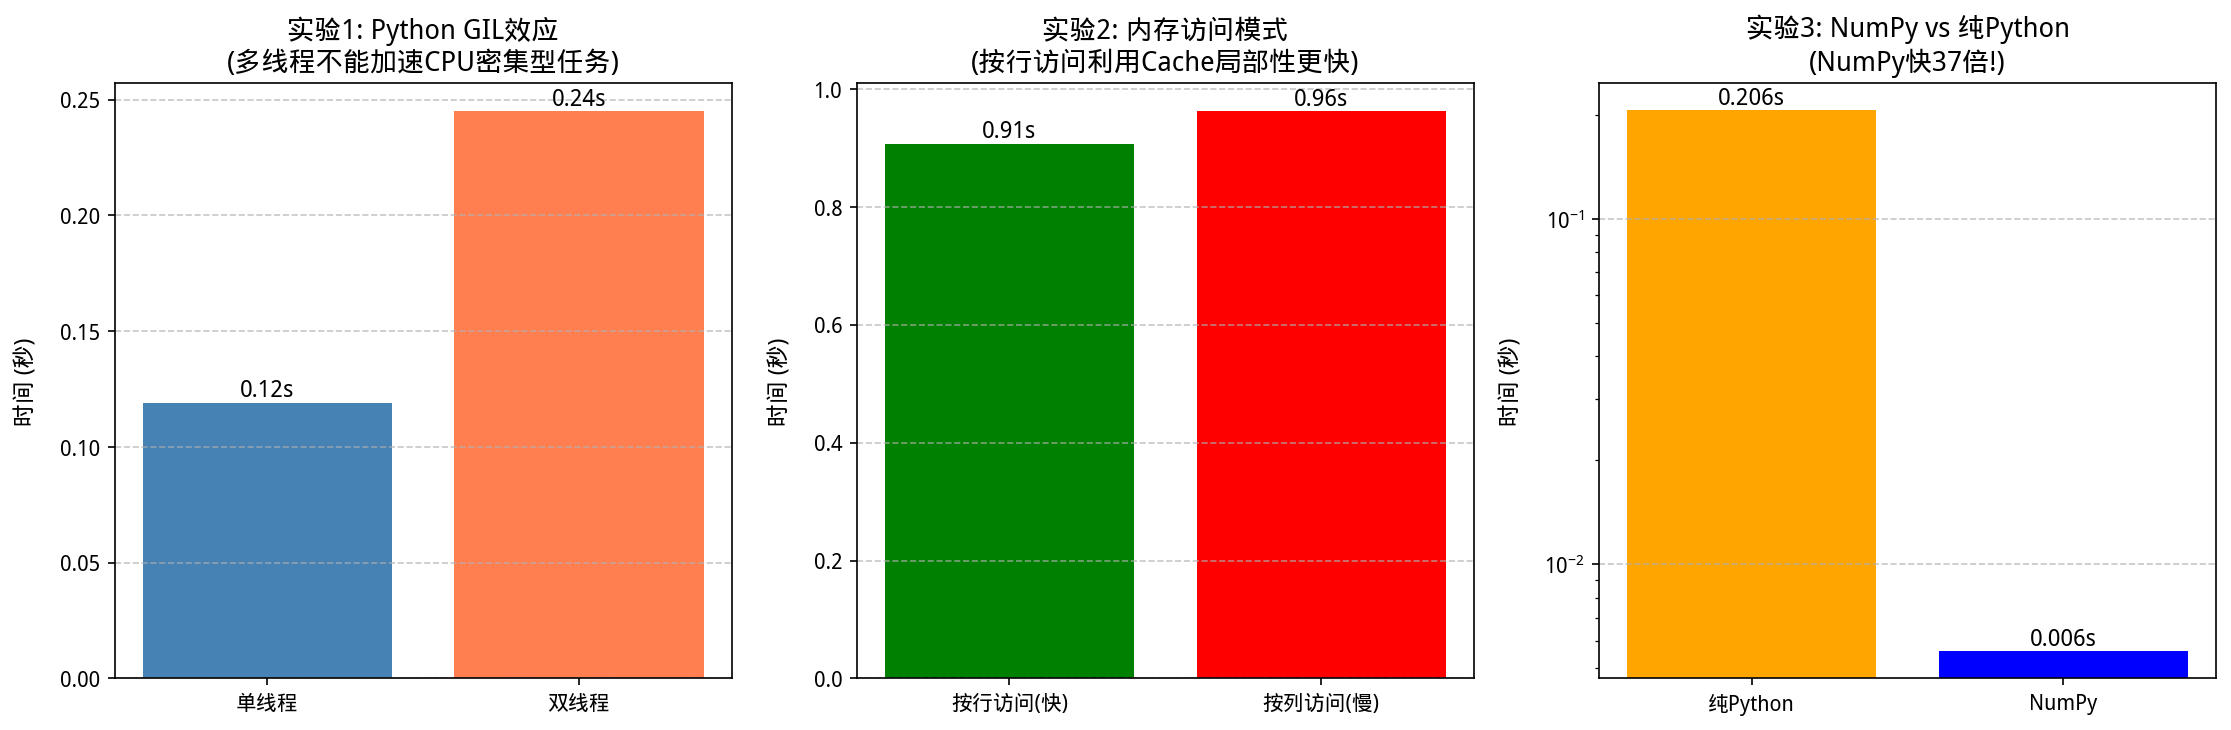
\includegraphics[width=0.95\textwidth]{figs/chap05_fig1.png}
\caption{Python性能优化实验：GIL对多线程的影响、缓存局部性的重要性、以及NumPy向量化的加速效果。左图显示Python多线程在CPU密集任务上受GIL限制，multiprocessing才能真正并行；中图展示行优先vs列优先遍历的性能差异（缓存局部性）；右图对比循环与向量化操作的速度——向量化可获得数十倍加速。}
\label{fig:chap05_python}
\end{figure}

\begin{figure}[htbp]
\centering
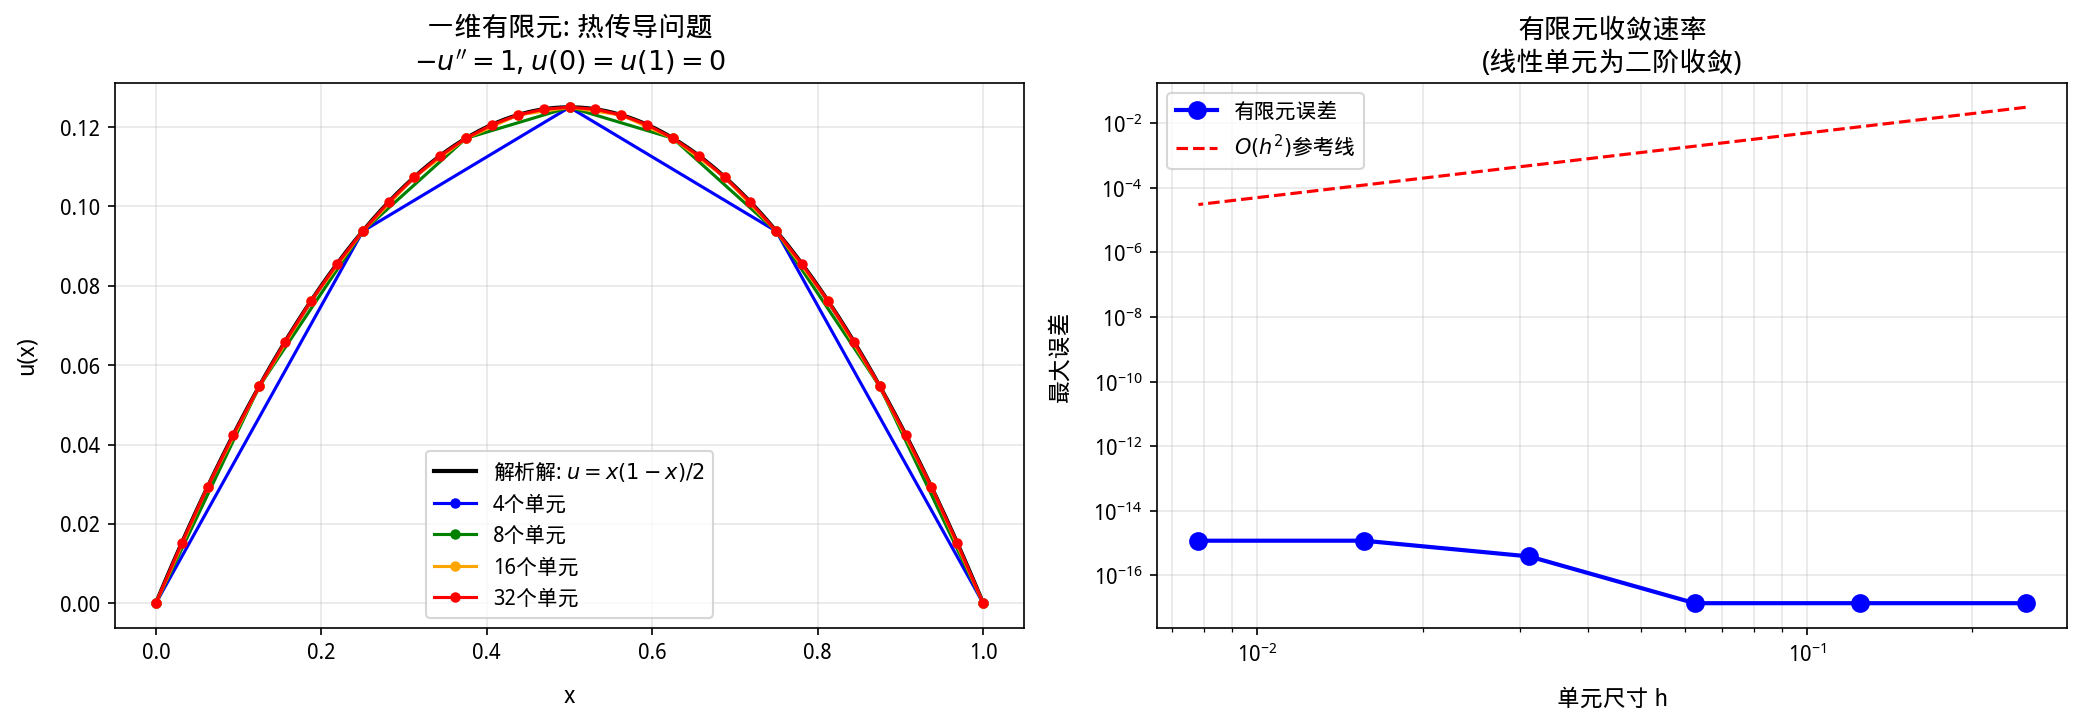
\includegraphics[width=0.95\textwidth]{figs/chap05_fig2.png}
\caption{一维有限元求解热传导问题。左图展示有限元解与解析解$u(x) = x(1-x)/2$的对比，二者几乎完全重合；中图显示刚度矩阵$K$的三对角稀疏结构——这源于帐篷函数的局部支撑性；右图展示网格细化时的收敛行为，验证了线性元的$O(h^2)$收敛阶。}
\label{fig:chap05_fem}
\end{figure}

% ------------------------------------------------------------------------------------
\section{本章小结}

\begin{enumerate}
    \item \textbf{核心思想}：有限元方法把无限维的变分问题转化为有限维的线性方程组 $KU = F$。
    
    \item \textbf{与有限差分的关系}：一维等价，二维开始分化；FEM 的优势在于处理复杂几何。
    
    \item \textbf{连续性}：$C^0$ 连续性保证能量有限；线性单元靠"两点定一线"自动满足连续性。
    
    \item \textbf{全局视角}：有限元解是全局"帐篷"基函数的线性叠加。
    
    \item \textbf{稀疏性}：基函数的局部支撑性导致刚度矩阵稀疏。
    
    \item \textbf{优化视角}：有限元 $\Leftrightarrow$ 能量最小化 $\Leftrightarrow$ 带约束的 QP 问题。
    
    \item \textbf{间断有限元}：放弃强制连续性，用约束/罚函数缝合，获得天然并行性。
\end{enumerate}

\begin{unification}[title=有限元：优化视角的大统一]
\begin{center}
\begin{tabular}{lll}
\toprule
\textbf{优化概念} & \textbf{有限元对应} & \textbf{物理意义} \\
\midrule
决策变量 & 节点值 $U_i$ & 物理量（温度/位移） \\
目标函数 & $\frac{1}{2}U^\top KU - F^\top U$ & 总势能 \\
等式约束 & Dirichlet 边界条件 & 固定边界 \\
拉格朗日乘子 & 边界反力 & 约束力 \\
罚函数 & 界面耦合项 & 虚拟弹簧 \\
\bottomrule
\end{tabular}
\end{center}

有限元不是孤立的数值技术，它是\textbf{变分原理}和\textbf{约束优化}在工程中的自然统一！

从第1章的拉格朗日乘子，到这里的有限元，$\lambda$ 始终扮演着"约束力"的角色。
\end{unification}


% ------------------------------------------------------------------------------------
\section{习题}

\paragraph{计算题}
\begin{enumerate}
    \item 用 2 个线性单元求解 $-u'' = 1$，$u(0) = u(1) = 0$。
    \begin{enumerate}
        \item 写出刚度矩阵 $K$ 和载荷向量 $F$
        \item 求解线性方程组，得到节点值 $U_1$
        \item 与精确解 $u(0.5) = 0.125$ 比较
    \end{enumerate}
    
    \item 用 4 个线性单元求解 $-u'' = \sin(\pi x)$，$u(0) = u(1) = 0$。
    \begin{enumerate}
        \item 计算载荷向量（需要积分 $\int \sin(\pi x) \phi_i dx$）
        \item 求解节点值
        \item 与精确解 $u(x) = \frac{\sin(\pi x)}{\pi^2}$ 比较
    \end{enumerate}
    
    \item 考虑非齐次边界条件：$-u'' = 0$，$u(0) = 0$，$u(1) = 1$。
    \begin{enumerate}
        \item 用 3 个单元建立有限元方程
        \item 用直接消去法处理边界条件
        \item 求解并验证结果是直线 $u(x) = x$
    \end{enumerate}
\end{enumerate}

\paragraph{证明题}
\begin{enumerate}
    \setcounter{enumi}{3}
    \item 证明刚度矩阵 $K$ 是对称的：$K_{ij} = K_{ji}$。
    
    \item 证明刚度矩阵 $K$ 是半正定的：$U^\top K U \geq 0$ 对所有 $U$ 成立。
    
    \item 证明有限元解 $u_h$ 是精确解 $u$ 在有限元空间中的"最佳逼近"：
    \[
    \int_0^1 (u_h' - u')^2 dx \leq \int_0^1 (v_h' - u')^2 dx \quad \forall v_h \in V_h
    \]
    （提示：这叫做 Galerkin 正交性）
\end{enumerate}

\paragraph{编程题}
\begin{enumerate}
    \setcounter{enumi}{6}
    \item 实现一维线性有限元：
    \begin{enumerate}
        \item 输入：区间 $[0, 1]$，单元数 $N$，源项 $f(x)$，边界值
        \item 输出：节点值向量 $U$
        \item 测试：$-u'' = 1$，$u(0) = u(1) = 0$
    \end{enumerate}
    
    \item 做收敛性实验：
    \begin{enumerate}
        \item 用 $N = 4, 8, 16, 32, 64$ 个单元求解
        \item 计算误差 $\|u - u_h\|_{L^2}$（用数值积分）
        \item 画 $\log(\text{误差})$ vs $\log(h)$ 的图，验证 $O(h^2)$ 收敛
    \end{enumerate}
    
    \item （挑战）实现二维三角形有限元：
    \begin{enumerate}
        \item 对单位正方形用三角形网格剖分
        \item 组装刚度矩阵和载荷向量
        \item 求解 $-\nabla^2 u = 1$，$u|_{\partial\Omega} = 0$
        \item 可视化数值解
    \end{enumerate}
\end{enumerate}

\paragraph{思考题}
\begin{enumerate}
    \setcounter{enumi}{9}
    \item 有限元方法和有限差分方法有什么本质区别？各有什么优缺点？
    
    \item 为什么有限元在工程中如此成功？它解决了工程师的什么痛点？
    
    \item 有限元方法与第13章的 PINN（物理信息神经网络）有什么联系和区别？
    
    \item 如果你要模拟一架飞机的应力分布，需要多少个有限元节点？这对计算机的要求是什么？
\end{enumerate}



% ====================================================================================
\section*{扩展阅读：大规模线性方程组的求解艺术}
\addcontentsline{toc}{section}{扩展阅读：大规模线性方程组的求解艺术}
% ====================================================================================

\begin{tcolorbox}[colback=gray!5, colframe=gray!50, title=本节导读]
有限元方法的最后一步是求解线性方程组 $KU = F$。这看起来很简单——不就是解个方程吗？

但当工程师模拟一架波音787的应力时，这个方程组可能有\textbf{上亿个未知数}。如何高效求解？答案涉及到一些深刻的数学概念：条件数、稀疏性、并行计算和预条件子。

更令人惊讶的是，这些概念在现代机器学习中同样重要——神经网络的训练本质上也是在求解大规模方程组！
\end{tcolorbox}

% ------------------------------------------------------------------------------------
\subsection*{一、条件数：方程组的"健康指标"}

\subsubsection*{一个令人困惑的现象}

考虑两个看起来很相似的方程组：

\begin{minipage}[t]{0.48\textwidth}
\textbf{方程组 A}
\[
\begin{pmatrix} 1 & 0 \\ 0 & 1 \end{pmatrix}
\begin{pmatrix} x \\ y \end{pmatrix}
= \begin{pmatrix} 1 \\ 1 \end{pmatrix}
\]
解：$x = 1, y = 1$

如果右边有小扰动 $(1.01, 0.99)$：

解变成 $x = 1.01, y = 0.99$

\textbf{扰动 1\%，解也变化 1\%}
\end{minipage}
\hfill
\begin{minipage}[t]{0.48\textwidth}
\textbf{方程组 B}
\[
\begin{pmatrix} 1 & 1 \\ 1 & 1.0001 \end{pmatrix}
\begin{pmatrix} x \\ y \end{pmatrix}
= \begin{pmatrix} 2 \\ 2.0001 \end{pmatrix}
\]
解：$x = 1, y = 1$

如果右边有小扰动 $(2.01, 2.0001)$：

解变成 $x = 101, y = -99$

\textbf{扰动 0.5\%，解变化 10000\%！}
\end{minipage}

\vspace{0.5cm}

为什么方程组 B 如此"敏感"？这就是\textbf{条件数}要回答的问题。

\subsubsection*{条件数的定义}

\begin{keyformula}[title=条件数]
矩阵 $A$ 的\textbf{条件数}定义为：
\begin{equation}
\kappa(A) = \|A\| \cdot \|A^{-1}\| = \frac{\sigma_{\max}(A)}{\sigma_{\min}(A)} = \frac{\text{最大奇异值}}{\text{最小奇异值}}
\end{equation}

对于对称正定矩阵（如有限元刚度矩阵）：
\begin{equation}
\kappa(K) = \frac{\lambda_{\max}(K)}{\lambda_{\min}(K)} = \frac{\text{最大特征值}}{\text{最小特征值}}
\end{equation}
\end{keyformula}

\textbf{条件数的意义}：

\begin{itemize}
    \item $\kappa \approx 1$：方程组"健康"，对扰动不敏感
    \item $\kappa \gg 1$：方程组"病态"，小扰动可能导致大误差
    \item $\kappa = \infty$：矩阵奇异，方程无唯一解
\end{itemize}

\begin{figure}[h]
\centering
\begin{tikzpicture}[scale=1.5]
    % 左边：良态矩阵
    \begin{scope}
        \node[font=\bfseries] at (1, 2.3) {良态 $\kappa \approx 1$};
        \draw[->] (0, 0) -- (2.2, 0) node[right] {$x$};
        \draw[->] (0, 0) -- (0, 2.2) node[above] {$y$};
        
        % 单位圆
        \draw[blue, thick] (1, 1) circle (0.7);
        \node[blue] at (1, 0.1) {输入扰动};
        
        % 输出也是圆（差不多大小）
        \draw[red, thick, dashed] (1, 1) ellipse (0.8 and 0.6);
        \node[red] at (1.8, 1.8) {输出误差};
    \end{scope}
    
    % 右边：病态矩阵
    \begin{scope}[xshift=4cm]
        \node[font=\bfseries] at (1, 2.3) {病态 $\kappa \gg 1$};
        \draw[->] (0, 0) -- (2.2, 0) node[right] {$x$};
        \draw[->] (0, 0) -- (0, 2.2) node[above] {$y$};
        
        % 单位圆
        \draw[blue, thick] (1, 1) circle (0.3);
        \node[blue] at (1, 0.5) {输入扰动};
        
        % 输出是扁长椭圆
        \draw[red, thick, dashed, rotate around={30:(1,1)}] (1, 1) ellipse (1.5 and 0.15);
        \node[red] at (2.2, 1.8) {输出误差};
        \node[red, font=\scriptsize] at (2.2, 1.5) {被放大！};
    \end{scope}
\end{tikzpicture}
\caption{条件数的几何意义：病态矩阵把圆形扰动拉成细长椭圆}
\end{figure}

\subsubsection*{有限元刚度矩阵的条件数}

有限元刚度矩阵的条件数与网格步长 $h$ 密切相关：

\begin{keytheorem}[title=刚度矩阵条件数估计]
对于一维 Poisson 方程的有限元刚度矩阵：
\begin{equation}
\kappa(K) \sim O\left(\frac{1}{h^2}\right)
\end{equation}

网格加密一倍（$h \to h/2$），条件数增大约 4 倍！
\end{keytheorem}

\textbf{为什么会这样？}

回顾刚度矩阵的三对角结构：
\[
K = \frac{1}{h}
\begin{pmatrix}
2 & -1 & & \\
-1 & 2 & -1 & \\
& \ddots & \ddots & \ddots \\
& & -1 & 2
\end{pmatrix}
\]

这个矩阵的特征值可以精确计算：
\begin{equation}
\lambda_k = \frac{4}{h} \sin^2\left(\frac{k\pi h}{2}\right), \quad k = 1, 2, \ldots, N-1
\end{equation}

\begin{itemize}
    \item 最小特征值：$\lambda_1 \approx \frac{4}{h} \cdot \frac{\pi^2 h^2}{4} = \pi^2 h$
    \item 最大特征值：$\lambda_{N-1} \approx \frac{4}{h}$
\end{itemize}

所以：
\[
\kappa(K) = \frac{\lambda_{\max}}{\lambda_{\min}} \approx \frac{4/h}{\pi^2 h} = \frac{4}{\pi^2 h^2} \sim O(h^{-2})
\]

\begin{physicalmeaning}
条件数与物理的关系：

\begin{itemize}
    \item \textbf{最大特征值}对应高频振动模式（相邻节点反向运动）——局部、快速
    \item \textbf{最小特征值}对应低频振动模式（整体缓慢变形）——全局、慢速
\end{itemize}

网格越细，高频和低频的差距越大，条件数越大。

这就像一根弦：基频（整体振动）和高次谐波（局部振动）的频率差距可以很大。
\end{physicalmeaning}

\subsubsection*{条件数对计算的影响}

条件数影响两件事：

\textbf{1. 直接求解的精度}

用 Gaussian 消元法求解时，舍入误差会被放大约 $\kappa$ 倍。

如果 $\kappa = 10^{10}$，双精度浮点数（约15位有效数字）只能保证约5位精度！

\textbf{2. 迭代求解的速度}

很多迭代算法（如共轭梯度法）的收敛速度与条件数直接相关：

\begin{equation}
\text{迭代次数} \sim O(\sqrt{\kappa})
\end{equation}

$\kappa = 10^6$ 意味着需要约 $1000$ 次迭代！

% ------------------------------------------------------------------------------------
\subsection*{二、稀疏矩阵：大自然的礼物}

\subsubsection*{什么是稀疏矩阵？}

\begin{definition}[稀疏矩阵]
如果一个 $n \times n$ 矩阵中非零元素的个数远小于 $n^2$（通常是 $O(n)$ 量级），我们称它为\textbf{稀疏矩阵}。
\end{definition}

有限元刚度矩阵就是典型的稀疏矩阵！

\begin{example}[波音787的有限元模型]
假设有 $n = 10^7$（一千万）个节点：

\begin{itemize}
    \item 稠密矩阵：$10^7 \times 10^7 = 10^{14}$ 个元素
        \begin{itemize}
            \item 存储：$10^{14} \times 8$ bytes $= 800$ TB（存不下！）
            \item 求解：$O(n^3) = 10^{21}$ 次运算（算不完！）
        \end{itemize}
    \item 稀疏矩阵：每行约 30 个非零元（三维问题）
        \begin{itemize}
            \item 存储：$3 \times 10^8$ 个非零元 $\approx 2.4$ GB（轻松！）
            \item 求解：使用稀疏求解器，可行！
        \end{itemize}
\end{itemize}
\end{example}

\subsubsection*{三对角矩阵：最简单的稀疏结构}

一维有限元产生的三对角矩阵是最简单的稀疏矩阵：

\[
K = \begin{pmatrix}
a_1 & c_1 & & & \\
b_2 & a_2 & c_2 & & \\
& b_3 & a_3 & c_3 & \\
& & \ddots & \ddots & \ddots \\
& & & b_n & a_n
\end{pmatrix}
\]

\textbf{Thomas 算法}（追赶法）可以在 $O(n)$ 时间内求解！

\noindent\textbf{算法：Thomas 算法（三对角系统求解）}

\medskip
\noindent\textbf{步骤：}

\begin{enumerate}
  \item \textbf{前向消元（从上到下）}
  \begin{enumerate}
      \item 对 $i=2,\dots,n$：
      \begin{itemize}
          \item $w = b_i / a_{i-1}$\hfill{\footnotesize（使第 $i$ 行以第 $i\!-\!1$ 行为基准做消元）}
          \item $a_i \leftarrow a_i - w \cdot c_{i-1}$\hfill{\footnotesize（更新主对角：消掉 $b_i$）}
          \item $f_i \leftarrow f_i - w \cdot f_{i-1}$\hfill{\footnotesize（右端项同样做线性消元）}
      \end{itemize}
  \end{enumerate}

  \item \textbf{回代（从下到上）}
  \begin{enumerate}
      \item 计算：$x_n = f_n / a_n$\hfill{\footnotesize（链条最末端最简单，从这里开始回传信息）}
      \item 对 $i = n-1, n-2, \dots, 1$：
      \begin{itemize}
          \item $x_i = (f_i - c_i \cdot x_{i+1}) / a_i$\hfill{\footnotesize（依次向上回代解）}
      \end{itemize}
  \end{enumerate}
\end{enumerate}

\begin{insightbox}
\textbf{Thomas 算法的本质}：

三对角系统就像一条链：
\[
\bullet - \bullet - \bullet - \bullet - \bullet
\]

每个节点只与相邻节点耦合。

前向消元将链条“一节节剪断”，回代将解“一节节传回”。

本质上就是一种线性结构的动态规划。
\end{insightbox}


\subsubsection*{带状矩阵与块三对角矩阵}

二维和三维问题的刚度矩阵虽然不是三对角，但仍有规律的稀疏结构：

\begin{figure}[h]
\centering
\begin{tikzpicture}[scale=0.55]

    % -------------------------------
    % 一维：三对角
    % -------------------------------
    \begin{scope}[xshift=0cm]
        \node[font=\bfseries] at (2.5, 6) {一维：三对角};
        \draw[gray] (0,0) rectangle (5,5);

        % 主对角
        \foreach \i in {0,...,4} {
            \fill[blue!60] (\i, 4-\i) rectangle ++(1,1);
        }
        % 上下对角
        \foreach \i in {0,...,3} {
            \fill[blue!30] (\i+1, 4-\i) rectangle ++(1,1);
            \fill[blue!30] (\i, 3-\i) rectangle ++(1,1);
        }

        \node at (2.5, -0.8) {\small 带宽 = 1};
    \end{scope}


    % -------------------------------
    % 二维：带状
    % -------------------------------
    \begin{scope}[xshift=8.5cm]
        \node[font=\bfseries] at (3, 6) {二维：带状};
        \draw[gray] (0,0) rectangle (6,6);

        % 主对角
        \foreach \i in {0,...,5} {
            \fill[blue!60] (\i, 5-\i) rectangle ++(1,1);
        }
        % 近对角
        \foreach \i in {0,...,4} {
            \fill[blue!30] (\i+1, 5-\i) rectangle ++(1,1);
            \fill[blue!30] (\i, 4-\i) rectangle ++(1,1);
        }
        % 远对角（来自另一方向）
        \foreach \i in {0,...,2} {
            \fill[blue!15] (\i+3, 5-\i) rectangle ++(1,1);
            \fill[blue!15] (\i, 2-\i) rectangle ++(1,1);
        }

        \node at (3, -0.8) {\small 带宽 $\approx \sqrt{n}$};
    \end{scope}


    % -------------------------------
    % 三维：更宽的带
    % -------------------------------
    \begin{scope}[xshift=17cm]
        \node[font=\bfseries] at (3.5, 6) {三维：更宽的带};
        \draw[gray] (0,0) rectangle (7,7);

        % 主对角
        \foreach \i in {0,...,6} {
            \fill[blue!60] (\i, 6-\i) rectangle ++(1,1);
        }

        % 逐步扩散的带状
        \foreach \d in {1,2,3} {
            \pgfmathsetmacro{\alpha}{60-15*\d}
            \foreach \i in {0,...,\numexpr6-\d} {
                \fill[blue!\alpha] (\i+\d, 6-\i) rectangle ++(1,1);
                \fill[blue!\alpha] (\i, 6-\i-\d) rectangle ++(1,1);
            }
        }

        \node at (3.5, -0.8) {\small 带宽 $\approx n^{2/3}$};
    \end{scope}

\end{tikzpicture}
\caption{不同维度问题的刚度矩阵稀疏结构}
\end{figure}


\textbf{带宽}决定了直接求解所需的计算量：

\begin{center}
\begin{tabular}{c|c|c|c}
\toprule
问题维度 & 带宽 $b$ & 求解复杂度 & $n = 10^6$ 时 \\
\midrule
一维 & $O(1)$ & $O(n)$ & $10^6$ 次运算 \\
二维 & $O(\sqrt{n})$ & $O(n \cdot b^2) = O(n^2)$ & $10^{12}$ 次运算 \\
三维 & $O(n^{2/3})$ & $O(n \cdot b^2) = O(n^{7/3})$ & $10^{14}$ 次运算 \\
\bottomrule
\end{tabular}
\end{center}

这就是为什么\textbf{大规模三维问题必须用迭代法}。

% ------------------------------------------------------------------------------------
\subsection*{三、并行计算：分而治之}

\subsubsection*{为什么三对角求解难以并行？}

Thomas 算法虽然快（$O(n)$），但它是\textbf{串行}的：

\begin{itemize}
    \item 前向消元：第 $i$ 步依赖第 $i-1$ 步的结果
    \item 回代：第 $i$ 步依赖第 $i+1$ 步的结果
\end{itemize}

就像多米诺骨牌，必须一个接一个倒下，不能跳跃！

\begin{figure}[h]
\centering
\begin{tikzpicture}[scale=0.8]
    % 串行
    \node[font=\bfseries] at (3, 2) {串行 Thomas 算法};
    \foreach \i in {1,...,6} {
        \draw[thick, fill=blue!30] (\i, 0) rectangle ++(0.6, 1);
        \node at (\i+0.3, 0.5) {\small $\i$};
    }
    \draw[->, thick, red] (1.3, 0.5) -- (1.7, 0.5);
    \draw[->, thick, red] (2.3, 0.5) -- (2.7, 0.5);
    \draw[->, thick, red] (3.3, 0.5) -- (3.7, 0.5);
    \draw[->, thick, red] (4.3, 0.5) -- (4.7, 0.5);
    \draw[->, thick, red] (5.3, 0.5) -- (5.7, 0.5);
    \node at (3.5, -0.8) {\small 必须按顺序执行};
\end{tikzpicture}
\end{figure}

\subsubsection*{域分解：把问题切开}

一个聪明的想法：把计算域\textbf{分成几块}，每块独立求解，然后把边界"缝合"起来。

\begin{figure}[h]
\centering
\begin{tikzpicture}[scale=1.2]
    % 原始问题
    \begin{scope}
        \node[font=\bfseries] at (2, 1.5) {原始问题};
        \draw[thick] (0, 0) -- (4, 0);
        \foreach \i in {0,...,8} {
            \fill (\i*0.5, 0) circle (2pt);
        }
        \node at (2, -0.5) {8个节点，一个方程组};
    \end{scope}
    
    % 箭头
    \draw[->, very thick] (4.5, 0) -- (5.5, 0);
    
    % 分解后
    \begin{scope}[xshift=6cm]
        \node[font=\bfseries] at (2, 1.5) {域分解};
        
        % 子域1
        \draw[thick, blue] (0, 0) -- (1.8, 0);
        \foreach \i in {0,...,3} {
            \fill[blue] (\i*0.5, 0) circle (2pt);
        }
        \node[blue] at (0.9, 0.4) {子域1};
        
        % 子域2
        \draw[thick, red] (2.2, 0) -- (4, 0);
        \foreach \i in {5,...,8} {
            \fill[red] (\i*0.5, 0) circle (2pt);
        }
        \node[red] at (3.1, 0.4) {子域2};
        
        % 界面
        \draw[thick, green!60!black, dashed] (1.8, -0.3) -- (2.2, -0.3);
        \fill[green!60!black] (2, 0) circle (3pt);
        \node[green!60!black] at (2, -0.7) {界面};
        
        \node at (2, -1.2) {两个小方程组 + 界面条件};
    \end{scope}
\end{tikzpicture}
\caption{域分解的基本思想}
\end{figure}

\subsubsection*{Schur 补：界面上的方程}

设原方程组为：
\[
\begin{pmatrix}
A_{11} & A_{12} & 0 \\
A_{21} & A_{22} & A_{23} \\
0 & A_{32} & A_{33}
\end{pmatrix}
\begin{pmatrix}
u_1 \\ u_\Gamma \\ u_2
\end{pmatrix}
=
\begin{pmatrix}
f_1 \\ f_\Gamma \\ f_2
\end{pmatrix}
\]

其中 $u_1, u_2$ 是两个子域的内部节点，$u_\Gamma$ 是界面节点。

从第一个和第三个方程解出 $u_1, u_2$（关于 $u_\Gamma$ 的函数），代入第二个方程：

\begin{equation}
\underbrace{\left(A_{22} - A_{21}A_{11}^{-1}A_{12} - A_{23}A_{33}^{-1}A_{32}\right)}_{S: \text{Schur 补}} u_\Gamma = \tilde{f}_\Gamma
\end{equation}


\paragraph{推导 Schur 补}

把矩阵方程展开成三个方程：
\begin{align}
A_{11} u_1 + A_{12} u_\Gamma &= f_1 \tag{子域1内部} \\
A_{21} u_1 + A_{22} u_\Gamma + A_{23} u_2 &= f_\Gamma \tag{界面} \\
A_{32} u_\Gamma + A_{33} u_2 &= f_2 \tag{子域2内部}
\end{align}

\textbf{第一步}：从方程(1)解出 $u_1$（把 $u_\Gamma$ 当作已知量）
\[
u_1 = A_{11}^{-1}(f_1 - A_{12} u_\Gamma)
\]

\textbf{第二步}：从方程(3)解出 $u_2$（把 $u_\Gamma$ 当作已知量）
\[
u_2 = A_{33}^{-1}(f_2 - A_{32} u_\Gamma)
\]

\textbf{第三步}：把 $u_1, u_2$ 代入方程(2)，消去内部自由度
\begin{align*}
A_{21} \cdot \underbrace{A_{11}^{-1}(f_1 - A_{12} u_\Gamma)}_{u_1} + A_{22} u_\Gamma + A_{23} \cdot \underbrace{A_{33}^{-1}(f_2 - A_{32} u_\Gamma)}_{u_2} &= f_\Gamma
\end{align*}

展开并整理（把 $u_\Gamma$ 的项放到左边，常数项放到右边）：
\[
\underbrace{\left(A_{22} - A_{21}A_{11}^{-1}A_{12} - A_{23}A_{33}^{-1}A_{32}\right)}_{S:\text{ Schur 补}} u_\Gamma = \underbrace{f_\Gamma - A_{21}A_{11}^{-1}f_1 - A_{23}A_{33}^{-1}f_2}_{\tilde{f}_\Gamma:\text{ 修正后的右端项}}
\]


\begin{keyformula}[title=Schur 补方法]
\begin{enumerate}
    \item \textbf{并行}：在每个子域上独立计算 $A_{11}^{-1}$ 和 $A_{33}^{-1}$
    \item \textbf{组装}：形成界面上的 Schur 补系统 $S u_\Gamma = \tilde{f}_\Gamma$
    \item \textbf{求解}：解这个小得多的界面方程
    \item \textbf{并行}：用 $u_\Gamma$ 回代得到各子域的解
\end{enumerate}
\end{keyformula}

\begin{physicalmeaning}
Schur 补的物理意义：

想象把一根弹簧链在中间切断，两边分别"凝缩"成等效刚度。

$S$ 就是界面上的\textbf{等效刚度}——它告诉你：如果界面位移是 $u_\Gamma$，界面上受到的力是多少。

这与第1章中消去部分变量得到约束力的想法完全一致！
\end{physicalmeaning}


\begin{insightbox}
\textbf{并行计算的智慧}：

串行算法追求的是\textbf{减少总工作量}。

并行算法追求的是\textbf{减少依赖深度}——即使总工作量增加，只要能并行就值得！

Schur补的总运算量比 Thomas 算法多，但它的\textbf{并行深度}是 $O(\log n)$，这使得在 GPU 上可以获得巨大加速。
\end{insightbox}

% ------------------------------------------------------------------------------------
\subsection*{四、预条件子：让迭代飞起来}

\subsubsection*{迭代法的基本思想}

当问题太大，直接求解不现实时，我们转向\textbf{迭代法}：

从一个初始猜测 $U^{(0)}$ 开始，逐步改进：
\[
U^{(0)} \to U^{(1)} \to U^{(2)} \to \cdots \to U^*
\]

\paragraph{最简单的迭代法：Jacobi 迭代}

考虑线性方程组 $KU = F$，写成分量形式：
\[
\sum_{j=1}^{n} K_{ij} U_j = F_i, \quad i = 1, 2, \ldots, n
\]

把第 $i$ 个方程中的 $U_i$ 单独拿出来：
\[
K_{ii} U_i + \sum_{j \neq i} K_{ij} U_j = F_i
\]

解出 $U_i$：
\[
U_i = \frac{1}{K_{ii}} \left( F_i - \sum_{j \neq i} K_{ij} U_j \right)
\]

\textbf{Jacobi 迭代}的想法：用旧的 $U^{(k)}$ 计算右边，得到新的 $U^{(k+1)}$：

\begin{tcolorbox}[colback=gray!5, colframe=gray!60, title=Jacobi 迭代]
\begin{equation}
U_i^{(k+1)} = \frac{1}{K_{ii}} \left( F_i - \sum_{j \neq i} K_{ij} U_j^{(k)} \right), \quad i = 1, 2, \ldots, n
\end{equation}

或者用矩阵形式：
\[
U^{(k+1)} = D^{-1}(F - (K-D)U^{(k)})
\]
其中 $D = \text{diag}(K)$ 是 $K$ 的对角部分。
\end{tcolorbox}

\paragraph{一个具体例子}

求解：
\[
\begin{pmatrix} 4 & 1 \\ 1 & 3 \end{pmatrix} \begin{pmatrix} U_1 \\ U_2 \end{pmatrix} = \begin{pmatrix} 1 \\ 2 \end{pmatrix}
\]

精确解是 $U_1 = 1/11 \approx 0.091$，$U_2 = 7/11 \approx 0.636$。

\textbf{Jacobi 迭代公式}：
\begin{align}
U_1^{(k+1)} &= \frac{1}{4}\left(1 - 1 \cdot U_2^{(k)}\right) = \frac{1 - U_2^{(k)}}{4} \\
U_2^{(k+1)} &= \frac{1}{3}\left(2 - 1 \cdot U_1^{(k)}\right) = \frac{2 - U_1^{(k)}}{3}
\end{align}

从 $U^{(0)} = (0, 0)$ 开始迭代：

\begin{center}
\begin{tabular}{c|c|c|c}
\toprule
迭代次数 $k$ & $U_1^{(k)}$ & $U_2^{(k)}$ & 误差 $\|U^{(k)} - U^*\|$ \\
\midrule
0 & 0 & 0 & 0.643 \\
1 & 0.250 & 0.667 & 0.162 \\
2 & 0.083 & 0.583 & 0.053 \\
3 & 0.104 & 0.639 & 0.013 \\
4 & 0.090 & 0.632 & 0.004 \\
5 & 0.092 & 0.637 & 0.001 \\
$\vdots$ & $\vdots$ & $\vdots$ & $\vdots$ \\
$\infty$ & 0.091 & 0.636 & 0 \\
\bottomrule
\end{tabular}
\end{center}

\begin{figure}[h]
\centering
\begin{tikzpicture}[scale=4]
    % 坐标轴
    \draw[->] (-0.1, 0) -- (0.35, 0) node[right] {$U_1$};
    \draw[->] (0, -0.1) -- (0, 0.8) node[above] {$U_2$};
    
    % 精确解
    \fill[red] (0.091, 0.636) circle (1pt);
    \node[red, above right] at (0.091, 0.636) {\small 精确解};
    
    % 迭代轨迹
    \draw[blue, thick, ->] (0, 0) -- (0.25, 0.667);
    \draw[blue, thick, ->] (0.25, 0.667) -- (0.083, 0.583);
    \draw[blue, thick, ->] (0.083, 0.583) -- (0.104, 0.639);
    \draw[blue, thick, ->] (0.104, 0.639) -- (0.090, 0.632);
    \draw[blue, thick, ->] (0.090, 0.632) -- (0.092, 0.637);
    
    % 起点
    \fill[blue] (0, 0) circle (1pt);
    \node[blue, below left] at (0, 0) {\small 起点};
\end{tikzpicture}
\caption{Jacobi 迭代的轨迹：螺旋式逼近精确解}
\end{figure}

\paragraph{Jacobi 迭代的物理直觉}

对于有限元方程，Jacobi 迭代有很好的物理解释：

\begin{physicalmeaning}
想象一个弹簧网络处于非平衡状态。

Jacobi 迭代的每一步：
\begin{enumerate}
    \item 看每个节点受到的"不平衡力"：$r_i = F_i - \sum_j K_{ij} U_j$（残差）
    \item 假设其他节点不动，只调整当前节点来平衡这个力
    \item 同时对所有节点做这个调整
\end{enumerate}

就像同时轻轻推动所有不平衡的节点，让系统逐渐趋于平衡。
\end{physicalmeaning}

\paragraph{Jacobi vs Gauss-Seidel}

Jacobi 迭代的一个"浪费"：计算 $U_i^{(k+1)}$ 时，我们已经算出了 $U_1^{(k+1)}, \ldots, U_{i-1}^{(k+1)}$，为什么不用最新的值？

\textbf{Gauss-Seidel 迭代}就是这个改进：
\[
U_i^{(k+1)} = \frac{1}{K_{ii}} \left( F_i - \sum_{j < i} K_{ij} U_j^{(k+1)} - \sum_{j > i} K_{ij} U_j^{(k)} \right)
\]

\begin{center}
\begin{tabular}{l|c|c}
\toprule
& \textbf{Jacobi} & \textbf{Gauss-Seidel} \\
\midrule
更新方式 & 同时更新所有分量 & 依次更新每个分量 \\
使用的值 & 全用旧值 $U^{(k)}$ & 用最新可用的值 \\
收敛速度 & 较慢 & 通常快一倍 \\
并行性 & \textbf{完美并行}（各分量独立） & 串行（有依赖） \\
\bottomrule
\end{tabular}
\end{center}

\begin{insightbox}
\textbf{Jacobi 在 GPU 时代的复兴}：

Gauss-Seidel 收敛更快，但它是串行的——计算 $U_i$ 必须等 $U_1, \ldots, U_{i-1}$ 算完。

Jacobi 虽然慢，但每个分量可以\textbf{独立计算}——完美适合 GPU 的数千个核心！

在现代并行硬件上，做 2 次 Jacobi 迭代可能比做 1 次 Gauss-Seidel 还快。
\end{insightbox}

\paragraph{Jacobi 迭代的收敛性}

Jacobi 迭代不总是收敛！收敛的条件与矩阵的性质有关。

\begin{keytheorem}[title=Jacobi 收敛的充分条件]
如果矩阵 $K$ 是\textbf{严格对角占优}的：
\[
|K_{ii}| > \sum_{j \neq i} |K_{ij}|, \quad \forall i
\]
即每行的对角元绝对值大于该行其他元素绝对值之和，则 Jacobi 迭代收敛。
\end{keytheorem}

好消息：有限元刚度矩阵通常满足这个条件（或接近满足），所以 Jacobi 迭代对有限元问题通常收敛。

\vspace{0.5cm}
现在我们可以介绍更高级的迭代法了：

最重要的迭代法之一是\textbf{共轭梯度法}（CG），它把求解 $KU = F$ 转化为最小化：
\[
\min_U \quad \frac{1}{2}U^\top K U - F^\top U
\]

\paragraph{从最速下降到共轭梯度}

最直接的想法是\textbf{最速下降法}：每一步沿着负梯度方向走。

目标函数 $J(U) = \frac{1}{2}U^\top K U - F^\top U$ 的梯度是：
\[
\nabla J = KU - F = -r
\]
其中 $r = F - KU$ 叫做\textbf{残差}（residual），它衡量当前解离真实解有多远。

\begin{figure}[h]
\centering
\begin{tikzpicture}[scale=1.0]
    % 最速下降
    \begin{scope}
        \node[font=\bfseries] at (2, 3.5) {最速下降法};
        \draw[->] (0, 0) -- (4, 0) node[right] {$U_1$};
        \draw[->] (0, 0) -- (0, 3) node[above] {$U_2$};
        % 椭圆等高线
        \draw[blue!30, rotate around={0:(2,1.5)}] (2, 1.5) ellipse (1.5 and 0.5);
        \draw[blue!50, rotate around={0:(2,1.5)}] (2, 1.5) ellipse (1.0 and 0.33);
        \draw[blue!70, rotate around={0:(2,1.5)}] (2, 1.5) ellipse (0.5 and 0.17);
        \fill[red] (2, 1.5) circle (2pt);
        % 锯齿路径
        \draw[->, thick, red] (0.8, 2.2) -- (1.5, 1.1);
        \draw[->, thick, red] (1.5, 1.1) -- (1.8, 1.8);
        \draw[->, thick, red] (1.8, 1.8) -- (1.95, 1.35);
        \draw[->, thick, red] (1.95, 1.35) -- (2.0, 1.55);
        \node at (2, -0.5) {\small 锯齿形，收敛慢};
    \end{scope}
    
    % 共轭梯度
    \begin{scope}[xshift=6cm]
        \node[font=\bfseries] at (2, 3.5) {共轭梯度法};
        \draw[->] (0, 0) -- (4, 0) node[right] {$U_1$};
        \draw[->] (0, 0) -- (0, 3) node[above] {$U_2$};
        % 椭圆等高线
        \draw[blue!30, rotate around={0:(2,1.5)}] (2, 1.5) ellipse (1.5 and 0.5);
        \draw[blue!50, rotate around={0:(2,1.5)}] (2, 1.5) ellipse (1.0 and 0.33);
        \draw[blue!70, rotate around={0:(2,1.5)}] (2, 1.5) ellipse (0.5 and 0.17);
        \fill[red] (2, 1.5) circle (2pt);
        % 直接路径
        \draw[->, thick, green!60!black] (0.8, 2.2) -- (1.5, 0.9);
        \draw[->, thick, green!60!black] (1.5, 0.9) -- (2, 1.5);
        \node at (2, -0.5) {\small 最多$n$步收敛！};
    \end{scope}
\end{tikzpicture}
\caption{最速下降法会"锯齿"前进，共轭梯度法选择更聪明的方向}
\end{figure}

最速下降法的问题：在窄长的"山谷"中会来回震荡，收敛很慢。

\paragraph{共轭方向的魔力}

共轭梯度法的核心思想：不要每次都沿梯度走，而是选择\textbf{互相"共轭"的方向}。

\begin{definition}[共轭方向]
两个向量 $p$ 和 $q$ 关于矩阵 $K$ \textbf{共轭}（或 $K$-正交），如果：
\[
p^\top K q = 0
\]
\end{definition}

为什么共轭方向好？如果我们有 $n$ 个互相共轭的方向 $p_1, p_2, \ldots, p_n$，那么：

\begin{itemize}
    \item 沿 $p_1$ 走到最优 $\Rightarrow$ 这个方向上的分量"搞定了"
    \item 再沿 $p_2$ 走到最优 $\Rightarrow$ \textbf{不会破坏} $p_1$ 方向上的最优性！
    \item 最多 $n$ 步，所有方向都搞定，到达全局最优
\end{itemize}

\begin{insightbox}
\textbf{共轭 vs 正交}：

普通正交：$p^\top q = 0$（在欧几里得内积下垂直）

$K$-共轭：$p^\top K q = 0$（在 $K$ 定义的内积下垂直）

对于对称正定矩阵 $K$，可以定义内积 $\langle p, q \rangle_K = p^\top K q$。

共轭方向就是在这个"变形"的内积下互相垂直的方向！
\end{insightbox}


\begin{tcolorbox}[colback=gray!5, colframe=gray!60, title=共轭梯度法（CG）]
\textbf{输入}：对称正定矩阵 $K$，右端向量 $F$，初始猜测 $U^{(0)}$

\textbf{初始化}：
\begin{align*}
r^{(0)} &= F - K U^{(0)} & \textcolor{gray}{\text{// 初始残差}} \\
p^{(0)} &= r^{(0)} & \textcolor{gray}{\text{// 初始搜索方向 = 负梯度方向}}
\end{align*}

\textbf{迭代}：对 $k = 0, 1, 2, \ldots$

\begin{enumerate}
    \item \textbf{计算步长}（沿 $p^{(k)}$ 走多远？）
    \[
    \alpha_k = \frac{(r^{(k)})^\top r^{(k)}}{(p^{(k)})^\top K p^{(k)}} \quad \textcolor{gray}{\text{// 使 $J(U^{(k)} + \alpha p^{(k)})$ 最小的 $\alpha$}}
    \]
    
    \item \textbf{更新解}
    \[
    U^{(k+1)} = U^{(k)} + \alpha_k p^{(k)} \quad \textcolor{gray}{\text{// 沿搜索方向前进}}
    \]
    
    \item \textbf{更新残差}
    \[
    r^{(k+1)} = r^{(k)} - \alpha_k K p^{(k)} \quad \textcolor{gray}{\text{// 不用重新算 $F - KU$，省一次矩阵乘法}}
    \]
    
    \item \textbf{检查收敛}：如果 $\|r^{(k+1)}\| < \epsilon$，停止
    
    \item \textbf{计算新方向}（关键：保证与之前所有方向共轭！）
    \[
    \beta_k = \frac{(r^{(k+1)})^\top r^{(k+1)}}{(r^{(k)})^\top r^{(k)}} \quad \textcolor{gray}{\text{// Gram-Schmidt 正交化的系数}}
    \]
    \[
    p^{(k+1)} = r^{(k+1)} + \beta_k p^{(k)} \quad \textcolor{gray}{\text{// 新方向 = 残差 + 旧方向的修正}}
    \]
\end{enumerate}
\end{tcolorbox}

\paragraph{为什么这个算法如此高效？}

\begin{enumerate}
    \item \textbf{每步只需一次矩阵-向量乘法}：计算 $Kp^{(k)}$，这是主要开销
    
    \item \textbf{短递归}：$p^{(k+1)}$ 只依赖于 $p^{(k)}$ 和 $r^{(k+1)}$，不需要存储所有历史方向
    
    \item \textbf{自动共轭}：通过巧妙的 $\beta_k$ 选择，新方向自动与所有旧方向共轭（这是 CG 的数学奇迹！）
    
    \item \textbf{理论上 $n$ 步精确收敛}：对于 $n \times n$ 的矩阵，最多 $n$ 步得到精确解
\end{enumerate}

\begin{physicalmeaning}
CG 的几何直觉：

想象你在一个椭球形的山谷里找最低点。

\begin{itemize}
    \item \textbf{最速下降}：每次沿最陡的方向走，但山谷是歪的，你会来回反弹
    \item \textbf{共轭梯度}：第一步沿最陡方向，之后每步都选一个"新维度"，保证不走回头路
\end{itemize}

就像在 $n$ 维空间里，你有 $n$ 个互相垂直的方向。每走一步就"锁定"一个维度，$n$ 步后所有维度都锁定，到达最低点！
\end{physicalmeaning}

\paragraph{一个简单例子}

求解 $KU = F$，其中：
\[
K = \begin{pmatrix} 4 & 1 \\ 1 & 3 \end{pmatrix}, \quad F = \begin{pmatrix} 1 \\ 2 \end{pmatrix}, \quad U^{(0)} = \begin{pmatrix} 0 \\ 0 \end{pmatrix}
\]

\textbf{初始化}：$r^{(0)} = F - KU^{(0)} = (1, 2)^\top$，$p^{(0)} = (1, 2)^\top$

\textbf{第一步}：
\begin{align*}
Kp^{(0)} &= \begin{pmatrix} 4 & 1 \\ 1 & 3 \end{pmatrix} \begin{pmatrix} 1 \\ 2 \end{pmatrix} = \begin{pmatrix} 6 \\ 7 \end{pmatrix} \\
\alpha_0 &= \frac{1^2 + 2^2}{1 \cdot 6 + 2 \cdot 7} = \frac{5}{20} = 0.25 \\
U^{(1)} &= (0, 0)^\top + 0.25 \cdot (1, 2)^\top = (0.25, 0.5)^\top \\
r^{(1)} &= (1, 2)^\top - 0.25 \cdot (6, 7)^\top = (-0.5, 0.25)^\top
\end{align*}

\textbf{第二步}：
\begin{align*}
\beta_0 &= \frac{(-0.5)^2 + 0.25^2}{1^2 + 2^2} = \frac{0.3125}{5} = 0.0625 \\
p^{(1)} &= (-0.5, 0.25)^\top + 0.0625 \cdot (1, 2)^\top = (-0.4375, 0.375)^\top
\end{align*}

继续迭代...对于 $2 \times 2$ 的问题，\textbf{最多2步}就能得到精确解！

\subsubsection*{共轭梯度法的收敛速度}

\begin{keytheorem}[title=CG 收敛速度]
共轭梯度法的误差满足：
\begin{equation}
\|U^{(k)} - U^*\|_K \leq 2 \left(\frac{\sqrt{\kappa} - 1}{\sqrt{\kappa} + 1}\right)^k \|U^{(0)} - U^*\|_K
\end{equation}

要使误差减少到 $\epsilon$，需要迭代次数：
\begin{equation}
k \sim O\left(\sqrt{\kappa} \log(1/\epsilon)\right)
\end{equation}
\end{keytheorem}

对于有限元问题，$\kappa \sim h^{-2}$，所以 $k \sim O(h^{-1}) = O(\sqrt{n})$。

$n = 10^6$ 时需要约 $1000$ 次迭代——太慢了！

\begin{insightbox}
\textbf{条件数的几何直觉：为什么扁椭圆让迭代法痛苦？}

想象你在一个山谷中寻找最低点。迭代法就像蒙着眼睛下山——每一步只能沿着当前位置最陡的方向走。

\textbf{情况1：圆形山谷}（条件数 $\kappa \approx 1$）
\begin{itemize}
    \item 等高线是同心圆
    \item 最陡方向始终指向谷底
    \item 一步到位！
\end{itemize}

\textbf{情况2：狭长山谷}（条件数 $\kappa \gg 1$）
\begin{itemize}
    \item 等高线是扁椭圆
    \item 最陡方向指向椭圆短轴，而非谷底
    \item 结果：来回zigzag，浪费大量迭代！
\end{itemize}

\textbf{预条件子的作用}：把扁椭圆"拉圆"！

数学上，如果原问题的海森矩阵是 $A$，预条件后变成 $M^{-1}A$。好的 $M$ 能让 $M^{-1}A$ 的特征值更集中，等高线更接近圆形。
\end{insightbox}

\subsubsection*{预条件：变换问题}

\textbf{预条件}的基本思想：  
不直接求解 $KU = F$，而是先将它“变换”成一个更容易求解的线性系统。

做法是选一个矩阵 $M$（称为\textbf{预条件子}），使得新系统
\[
(M^{-1}K)U = M^{-1}F
\]
的\textbf{条件数比原系统小}，从而使迭代法收敛更快。

\textbf{好的预条件子应满足：}

\begin{itemize}
    \item $M^{-1}K$ 的条件数要小（这样迭代法收敛快）
    \item $M^{-1}v$ 要容易计算（每步迭代的代价低）
\end{itemize}

这两个要求本质上是矛盾的：

- 如果让 $M$ 与 $K$ 非常接近，那么 $M^{-1}K$ 的条件数就会非常理想（甚至当 $M = K$ 时条件数为 1）

- 但这时计算 $M^{-1}$ 本身就和解原问题一样困难，因此完全没有意义

因此，一个实用的预条件子必须在“逼近 $K$”（改善条件数）和“计算容易”（代价低）之间取得折中。

\subsubsection*{常见的预条件子}

\begin{center}
\renewcommand{\arraystretch}{1.5}
\begin{tabular}{l|c|c|l}
\toprule
预条件子 & $\kappa(M^{-1}K)$ & 每步代价 & 特点 \\
\midrule
无（$M = I$） & $O(h^{-2})$ & $O(1)$ & 基准 \\
Jacobi（$M = \text{diag}(K)$） & $O(h^{-2})$ & $O(n)$ & 简单，但改善有限 \\
不完全 LU (ILU) & $O(h^{-1})$ & $O(n)$ & 实用，通用 \\
多重网格 (MG) & $O(1)$! & $O(n)$ & 最优，但需要网格层次 \\
\bottomrule
\end{tabular}
\end{center}

\subsubsection*{多重网格：最优预条件子}

多重网格是有限元问题的"终极武器"——它能把条件数降到 $O(1)$！

但这个方法初看很神秘，让我们从一个具体问题开始理解它。

\paragraph{一个令人困惑的现象}

用 Jacobi 迭代求解有限元方程 $KU = F$，观察误差的变化：

\begin{figure}[h]
\centering
\begin{tikzpicture}[scale=0.9]
    % 初始误差
    \begin{scope}
        \node[font=\bfseries] at (2, 1.8) {初始误差};
        \draw[->] (0, 0) -- (4.2, 0) node[right] {\small $x$};
        \draw[->] (0, -1) -- (0, 1.2);
        \draw[blue, thick, domain=0:4, samples=100] plot (\x, {0.5*sin(30*\x) + 0.4*sin(540*\x)});
        \node[blue] at (2, -1.5) {\small 低频 + 高频混合};
    \end{scope}
    
    % 10次迭代后
    \begin{scope}[xshift=5.5cm]
        \node[font=\bfseries] at (2, 1.8) {10次 Jacobi 后};
        \draw[->] (0, 0) -- (4.2, 0) node[right] {\small $x$};
        \draw[->] (0, -1) -- (0, 1.2);
        \draw[red, thick, domain=0:4, samples=100] plot (\x, {0.5*sin(30*\x) + 0.05*sin(540*\x)});
        \node[red] at (2, -1.5) {\small 高频消失了，低频还在！};
    \end{scope}
\end{tikzpicture}
\caption{Jacobi 迭代快速消除高频误差，但对低频误差无能为力}
\end{figure}

\textbf{观察}：
\begin{itemize}
    \item 高频误差（振荡剧烈的部分）：几次迭代就消失了 ✓
    \item 低频误差（缓慢变化的部分）：迭代几百次还在！✗
\end{itemize}

这就是 Jacobi/Gauss-Seidel 等简单迭代法的通病：\textbf{只擅长消除高频，对低频束手无策}。

\paragraph{关键洞察：低频是相对的！}

现在是多重网格的灵魂时刻：

\begin{figure}[h]
\centering
\begin{tikzpicture}[scale=0.85]
    % 细网格上的低频
    \begin{scope}
        \node[font=\bfseries] at (2, 2) {细网格（16个点）};
        \draw[thick] (0, 0) -- (4, 0);
        \foreach \i in {0,...,16} {
            \fill (\i*0.25, 0) circle (1.5pt);
        }
        % 低频波
        \draw[red, very thick, domain=0:4, samples=50] plot (\x, {0.6*sin(45*\x)});
        \node[red] at (5.2, 0.4) {\small "低频"};
        \node at (2, -0.8) {\small 波长 = 8个网格间距};
    \end{scope}
    
    % 箭头
    \draw[->, ultra thick, blue] (2, -1.3) -- (2, -2.2);
    \node[blue, right] at (2.1, -1.75) {限制到粗网格};
    
    % 粗网格上变成高频
    \begin{scope}[yshift=-4cm]
        \node[font=\bfseries] at (2, 2) {粗网格（4个点）};
        \draw[thick] (0, 0) -- (4, 0);
        \foreach \i in {0,...,4} {
            \fill (\i, 0) circle (2.5pt);
        }
        % 同样的波，但现在是高频
        \draw[green!60!black, very thick, domain=0:4, samples=50] plot (\x, {0.6*sin(45*\x)});
        \node[green!60!black] at (5.2, 0.4) {\small "高频"!};
        \node at (2, -0.8) {\small 波长 = 2个网格间距};
    \end{scope}
\end{tikzpicture}
\caption{同一个波，在细网格上是"低频"，在粗网格上变成"高频"！}
\end{figure}

\begin{insightbox}
\textbf{多重网格的核心思想}：

细网格上的低频误差 $\xrightarrow{\text{限制}}$ 粗网格上的高频误差 $\xrightarrow{\text{Jacobi}}$ 快速消除！

这就像换一把尺子：用细尺子量不准的东西，换把粗尺子反而能量准。
\end{insightbox}

\begin{tcolorbox}[colback=gray!5, colframe=gray!60, title=两层网格算法（Two-Grid）]
\textbf{目标}：在细网格上求解 $K_h u_h = f_h$

\begin{enumerate}
    \item \textbf{预光滑}（Pre-smoothing）
    \begin{itemize}
        \item 在细网格上做几次 Jacobi 迭代
        \item \textcolor{gray}{// 消除高频误差，剩下光滑的低频误差}
    \end{itemize}
    
    \item \textbf{计算残差}
    \[
    r_h = f_h - K_h u_h \quad \textcolor{gray}{\text{// 当前解的"差多少"}}
    \]
    
    \item \textbf{限制到粗网格}（Restriction）
    \[
    r_H = R \cdot r_h \quad \textcolor{gray}{\text{// 把残差"投影"到粗网格}}
    \]
    这里 $R$ 是限制算子，最简单的是取相邻细网格点的平均。
    
    \item \textbf{在粗网格上求解误差方程}
    \[
    K_H e_H = r_H \quad \textcolor{gray}{\text{// 粗网格问题规模小，可以直接解或递归}}
    \]
    
    \item \textbf{插值回细网格}（Prolongation）
    \[
    e_h = P \cdot e_H \quad \textcolor{gray}{\text{// 把粗网格的修正"插值"回细网格}}
    \]
    这里 $P$ 是插值算子，通常用线性插值。
    
    \item \textbf{修正细网格解}
    \[
    u_h \leftarrow u_h + e_h \quad \textcolor{gray}{\text{// 加上粗网格算出的修正量}}
    \]
    
    \item \textbf{后光滑}（Post-smoothing）
    \begin{itemize}
        \item 再做几次 Jacobi 迭代 \textcolor{gray}{// 消除插值引入的高频误差}
    \end{itemize}
\end{enumerate}
\end{tcolorbox}

\paragraph{一个具体的数值例子}

求解一维问题 $-u'' = 1$，$u(0) = u(1) = 0$，用两层网格。

\textbf{设置}：
\begin{itemize}
    \item 细网格：$h = 1/8$，7个内部节点
    \item 粗网格：$H = 1/4$，3个内部节点
\end{itemize}

\begin{figure}[h]
\centering
\begin{tikzpicture}[scale=1.2]
    % 细网格
    \begin{scope}
        \node at (-1, 0) {细网格};
        \draw[thick] (0, 0) -- (5.6, 0);
        \foreach \i in {0,...,8} {
            \fill (\i*0.7, 0) circle (2pt);
            \node[below, font=\scriptsize] at (\i*0.7, -0.15) {$\i$};
        }
    \end{scope}
    
    % 粗网格
    \begin{scope}[yshift=-1.5cm]
        \node at (-1, 0) {粗网格};
        \draw[thick] (0, 0) -- (5.6, 0);
        \foreach \i in {0,...,4} {
            \fill (\i*1.4, 0) circle (3pt);
            \node[below, font=\scriptsize] at (\i*1.4, -0.15) {$\i$};
        }
    \end{scope}
    
    % 限制箭头
    \draw[->, blue, thick] (0.7, -0.3) -- (0, -1.2);
    \draw[->, blue, thick] (1.4, -0.3) -- (1.4, -1.2);
    \draw[->, blue, thick] (2.1, -0.3) -- (1.4, -1.2);
    
    \draw[->, blue, thick] (2.1, -0.3) -- (2.8, -1.2);
    \draw[->, blue, thick] (2.8, -0.3) -- (2.8, -1.2);
    \draw[->, blue, thick] (3.5, -0.3) -- (2.8, -1.2);
    
    \node[blue] at (6.5, -0.7) {限制 $R$};
\end{tikzpicture}
\caption{细网格节点到粗网格节点的对应关系}
\end{figure}

\textbf{限制算子}（全加权）：
\[
(R \cdot r_h)_i = \frac{1}{4}r_{2i-1} + \frac{1}{2}r_{2i} + \frac{1}{4}r_{2i+1}
\]
即：粗网格点的值 = 对应细网格点及其邻居的加权平均。

\textbf{插值算子}（线性插值）：
\[
(P \cdot e_H)_{2i} = e_i, \quad (P \cdot e_H)_{2i+1} = \frac{1}{2}(e_i + e_{i+1})
\]
即：粗网格点直接拷贝，中间点取两边平均。

\paragraph{为什么收敛这么快？}

\begin{center}
\renewcommand{\arraystretch}{1.3}
\begin{tabular}{l|c|c}
\toprule
\textbf{误差类型} & \textbf{处理方式} & \textbf{效果} \\
\midrule
细网格高频 & 预光滑（Jacobi） & 几次迭代消除 \\
细网格低频 & 限制到粗网格$\to$变成高频$\to$Jacobi消除 & 几次迭代消除 \\
更低的频率 & 继续限制到更粗的网格... & 递归处理 \\
\bottomrule
\end{tabular}
\end{center}

每种频率的误差都在\textbf{它最容易被消除的尺度上}被处理！

\paragraph{V-Cycle：递归的多重网格}

两层网格可以推广到多层——这就是 V-Cycle：

\begin{figure}[h]
\centering
\begin{tikzpicture}[scale=0.8]
    % V-cycle 示意图
    \node[draw, fill=blue!20, minimum width=1.5cm] (L0a) at (0, 0) {细网格};
    \node[draw, fill=blue!30, minimum width=1.2cm] (L1a) at (-1.5, -1.5) {中网格};
    \node[draw, fill=blue!40, minimum width=0.9cm] (L2) at (-3, -3) {粗网格};
    \node[draw, fill=blue!30, minimum width=1.2cm] (L1b) at (-1.5, -4.5) {中网格};
    \node[draw, fill=blue!20, minimum width=1.5cm] (L0b) at (0, -6) {细网格};
    
    % 箭头
    \draw[->, thick] (L0a) -- (L1a) node[midway, left] {\small 光滑+限制};
    \draw[->, thick] (L1a) -- (L2) node[midway, left] {\small 光滑+限制};
    \draw[->, thick] (L2) -- (L1b) node[midway, left] {\small 求解+插值};
    \draw[->, thick] (L1b) -- (L0b) node[midway, left] {\small 光滑+插值};
    
    % V 形状标注
    \draw[red, dashed, thick] (0.8, 0) -- (-3.8, -3) -- (0.8, -6);
    \node[red] at (2, -3) {\Large V-Cycle};
\end{tikzpicture}
\caption{V-Cycle：一路向下限制，到最粗层直接求解，再一路向上插值}
\end{figure}

\begin{keytheorem}[title=多重网格复杂度]
一次完整的多重网格 V-cycle：
\begin{itemize}
    \item \textbf{时间复杂度}：$O(n)$
    
    \textcolor{gray}{为什么？每层的工作量是 $n, n/2, n/4, \ldots$，总和 $\approx 2n = O(n)$}
    
    \item \textbf{收敛因子}：$\rho < 1$（与 $h$ 无关！）
    
    \textcolor{gray}{为什么？每种频率的误差都被高效处理，没有"漏网之鱼"}
\end{itemize}

这意味着：\textbf{解一个 $10^6$ 节点的问题和 $10^3$ 节点的问题，迭代次数几乎一样}！
\end{keytheorem}

\paragraph{数值验证}

用 CG（共轭梯度）求解有限元方程，对比不同预条件子：

\begin{center}
\renewcommand{\arraystretch}{1.3}
\begin{tabular}{l|c|c|c|c}
\toprule
\textbf{网格大小} & \textbf{无预条件} & \textbf{Jacobi} & \textbf{ILU} & \textbf{多重网格} \\
\midrule
$32 \times 32$ & 89 次 & 67 次 & 23 次 & 7 次 \\
$64 \times 64$ & 170 次 & 130 次 & 35 次 & 7 次 \\
$128 \times 128$ & 330 次 & 250 次 & 52 次 & 8 次 \\
$256 \times 256$ & 650 次 & 500 次 & 78 次 & 8 次 \\
\bottomrule
\end{tabular}
\end{center}

\textbf{观察}：
\begin{itemize}
    \item 无预条件/Jacobi：迭代次数随网格加密而增长（$\sim O(\sqrt{n})$）
    \item 多重网格：迭代次数\textbf{几乎不变}！这就是 $O(1)$ 条件数的威力
\end{itemize}

% 代码演示结果
\begin{figure}[htbp]
\centering
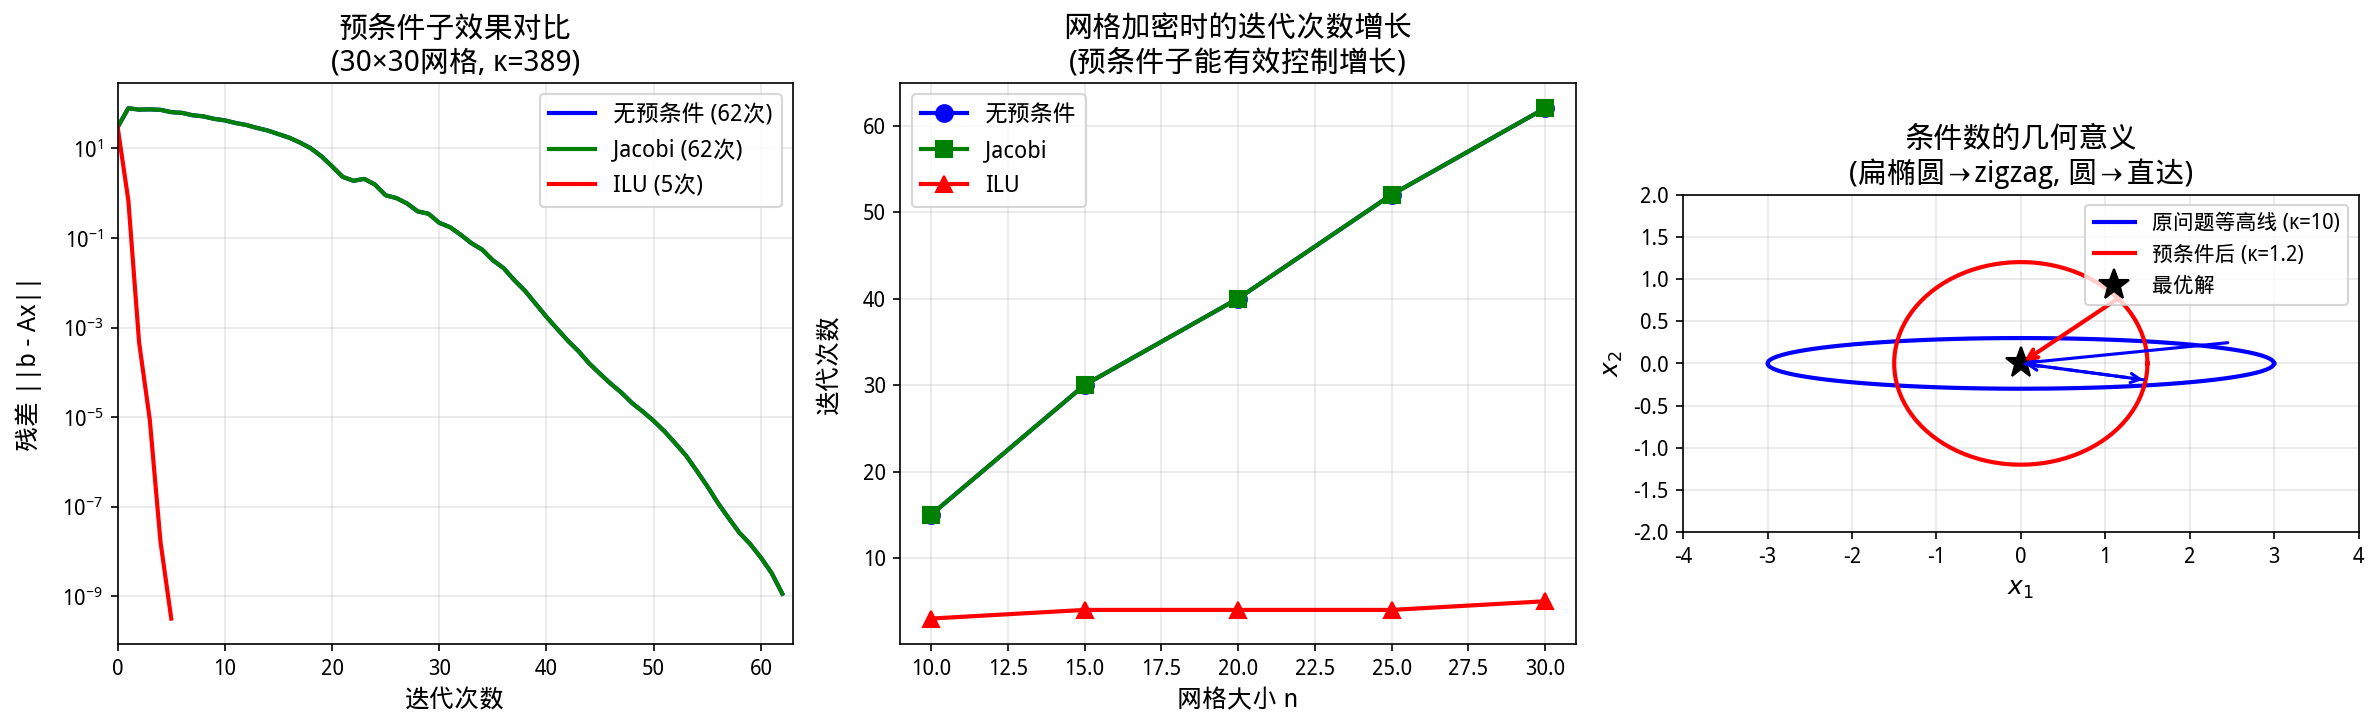
\includegraphics[width=0.95\textwidth]{figs/chap05_fig3.png}
\caption{预条件子效果的实验验证（1行3列）。\textbf{左图}：共轭梯度法收敛曲线对比——无预条件（蓝）、Jacobi预条件（绿）、ILU预条件（红），ILU只需约1/3的迭代次数；\textbf{中图}：网格加密时迭代次数的增长趋势——无预条件和Jacobi迭代次数线性增长，而ILU增长明显更慢；\textbf{右图}：条件数的几何意义——扁椭圆（高条件数）导致zigzag路径，圆形（低条件数）可以直达最优解。代码见 \texttt{code/chap05\_performance.py}。}
\label{fig:preconditioner}
\end{figure}

% ------------------------------------------------------------------------------------
\section*{扩展阅读：CPU 并行计算的真正含义}
\addcontentsline{toc}{section}{扩展阅读：CPU 并行计算的真正含义}

在学习数值计算和科学编程之前，初学者常常会问这样一个问题：

\begin{quote}
"为什么同样是一行代码，有的写法能快几十倍？为什么老师总让我用 NumPy，不要自己写循环？"
\end{quote}

要回答这个问题，我们必须从最基础的地方开始：CPU 是怎样执行程序的？它在什么情况下会变快、在什么情况下会变慢？这部分内容看似属于"计算机系统结构"，但它和我们写出高效代码息息相关。

为了让你真正"看得见"CPU 在做什么，我们会边讲概念边给出小实验。你可以在自己的电脑上立即验证这些现象，而不只是听一堆抽象的术语。

%==============================================================================
\subsection*{程序、进程、线程：你的电脑到底是怎样跑代码的？}
%==============================================================================

我们先从最核心的三个概念讲起。这三个词你可能早就听过，但很多人分不清它们的区别。

\paragraph{程序是什么？}

\textbf{程序（Program）}就是硬盘上的文件——一个 \verb|.exe|、一个 \verb|.py|、一个 \verb|.out|——本质上是一堆指令，静静地躺在那里，还没有执行。

打个比方：程序就像一本菜谱摆在书架上。你不动手做饭，它不会自己飘出味道来。

\paragraph{进程是什么？}

\textbf{进程（Process）}就是程序"开始执行"之后的样子。当你双击一个程序、或者在命令行输入 \verb|python xxx.py| 回车的那一刻，操作系统就会为这个程序创建一个进程。

进程有什么特点呢？它有：
\begin{itemize}
    \item 自己独立的内存空间（别的进程看不到、也改不了）
    \item 自己的变量、数据结构
    \item 自己的一套运行状态
\end{itemize}

继续用做饭来比喻：进程就是"你正在做菜"这件事本身。你占用了一整个厨房，锅、刀、案板、冰箱里的食材，都是你独占的。隔壁厨房在做什么菜，和你没关系。

\paragraph{线程是什么？}

\textbf{线程（Thread）}是进程内部的"执行路线"，或者说是"干活的小工"。一个进程可以同时雇好几个小工，让他们并行地帮你做事。

关键区别在于：同一个进程里的多个线程，\textbf{共享同一片内存空间}。它们可以直接读写同样的变量。

用厨房的比喻来说：
\begin{itemize}
    \item 一个进程是一家餐厅的厨房
    \item 线程是厨房里的多个厨师
    \item 厨师们共享同一个冰箱、同一套锅碗瓢盆（共享内存）
    \item 但不同餐厅的厨房是完全隔开的（进程之间隔离）
\end{itemize}

\begin{figure}[h]
\centering
\begin{tikzpicture}[scale=0.85]
    % 进程1
    \draw[thick, fill=blue!10, rounded corners] (0, 0) rectangle (5, 4);
    \node[font=\bfseries] at (2.5, 3.6) {进程 A（独立内存空间）};
    
    % 内存区域
    \draw[fill=yellow!20] (0.3, 2.2) rectangle (4.7, 3.2);
    \node[font=\small] at (2.5, 2.7) {共享内存：堆、全局变量};
    
    % A 的线程
    \foreach \x/\name in {0.5/线程1,2.1/线程2,3.7/线程3}{
        \draw[fill=green!30] (\x,0.5) rectangle ++(1.3,1.5);
        \node[font=\small, align=center] at (\x+0.65,1.25) {\name\\栈};
    }

    % 进程2
    \draw[thick, fill=red!10, rounded corners] (6, 0) rectangle (11, 4);
    \node[font=\bfseries] at (8.5, 3.6) {进程 B（独立内存空间）};
    \draw[fill=yellow!20] (6.3, 2.2) rectangle (10.7, 3.2);
    \node[font=\small] at (8.5, 2.7) {自己的内存};

    \foreach \x/\name in {6.5/线程1,8.2/线程2,9.9/线程3}{
        \draw[fill=orange!30] (\x,0.5) rectangle ++(1.3,1.5);
        \node[font=\small,align=center] at (\x+0.65,1.25) {\name\\栈};
    }

    % 隔离线
    \draw[ultra thick, red, dashed] (5.5,-0.5) -- (5.5,4.5);
    \node[red, font=\small] at (5.5,-0.8) {内存隔离};
\end{tikzpicture}
\caption{进程与线程的关系：进程之间相互隔离，而同一进程内的线程共享内存}
\end{figure}

下面这张表总结了进程和线程的主要区别：

\begin{center}
\renewcommand{\arraystretch}{1.3}
\begin{tabular}{l|l|l}
\toprule
\textbf{特性} & \textbf{进程} & \textbf{线程} \\
\midrule
内存空间 & 独立，互不共享 & 共享同一进程的内存 \\
创建开销 & 较大（需申请整块内存） & 较小（主要是栈空间） \\
通信方式 & 需要特殊机制（管道、共享内存等） & 直接读写共享变量 \\
崩溃影响 & 一个进程挂了，其他不受影响 & 一个线程挂了，整个进程可能崩溃 \\
典型应用 & 浏览器的多个标签页 & 一个程序内部的并行计算 \\
\bottomrule
\end{tabular}
\end{center}

%------------------------------------------------------------------------------
\paragraph{你可以自己做的小实验 1：Python 多线程为什么不快？}
%------------------------------------------------------------------------------

把下面的代码复制到你的电脑上运行一下：

\begin{lstlisting}[style=teaching, language=Python]
import threading
import time

def count():
    """一个简单的计数任务"""
    n = 0
    for _ in range(50_000_000):
        n += 1

# 先测试单线程
print("测试单线程...")
t0 = time.time()
count()
print(f"单线程耗时: {time.time() - t0:.2f} 秒")

# 再测试双线程
print("\n测试双线程...")
t0 = time.time()
t1 = threading.Thread(target=count)
t2 = threading.Thread(target=count)
t1.start()
t2.start()
t1.join()
t2.join()
print(f"双线程耗时: {time.time() - t0:.2f} 秒")
\end{lstlisting}

运行之后，你大概率会看到一个让人困惑的结果：

\begin{itemize}
    \item 单线程：大约 2--3 秒
    \item 双线程：大约 2--4 秒，甚至更慢！
\end{itemize}

这是怎么回事？开了两个线程，不是应该快一倍吗？

答案是：Python（准确说是 CPython 解释器）有一个特殊的设计叫 \textbf{GIL}（Global Interpreter Lock，全局解释器锁）。它规定：\textbf{同一时刻只能有一个线程在执行 Python 字节码}。

换句话说，即使你开了 10 个线程，Python 解释器也会让它们排队、轮流执行，而不是真正的并行。

这个实验让你亲眼看到了 GIL 的影响。后面我们会讲怎么绑过它。

%==============================================================================
\subsection*{内存层次：为什么有些代码能快 10 倍、100 倍？}
%==============================================================================

当老师说"访问 L1 Cache 是 1 纳秒，访问主内存是 100 纳秒"的时候，初学者往往没有感觉。1 纳秒是什么？100 纳秒又是什么？快还是慢？

我们换一个更直观的比喻。

\marginnote{
\textbf{小故事：}\\
1957 年，IBM 704 计算机的工程师们发现一个问题：CPU 算得太快，常常在"等"内存慢腾腾地把数据送过来。\\
于是他们在 CPU 旁边加了一小块极快的存储器，专门存最近用过的数据——这就是 Cache（高速缓存）的前身。\\
没想到，这个当年的"小补丁"后来成了所有现代处理器的标配设计。
}

想象一下你坐在办公桌前工作：
\begin{itemize}
    \item \textbf{寄存器}（$<1$ ns）：就像你手边的便签纸，伸手就能拿到
    \item \textbf{L1 Cache}（$\sim 1$ ns）：就像桌上的文件夹，抬手就能翻开
    \item \textbf{L2/L3 Cache}（几 ns--十几 ns）：就像抽屉里的资料，需要弯腰去拿
    \item \textbf{主内存 RAM}（$\sim 100$ ns）：就像走去隔壁房间的档案柜取文件
    \item \textbf{SSD 硬盘}（$\sim 100$ $\mu$s）：就像开车去另一栋楼的仓库取东西
\end{itemize}

现在你明白了吧？如果你的程序总是要"开车去仓库"，而别人的程序只需要"翻桌上的文件夹"，速度差别当然是天壤之别。

\begin{center}
\renewcommand{\arraystretch}{1.3}
\begin{tabular}{l|r|r|l}
\toprule
\textbf{层次} & \textbf{延迟（量级）} & \textbf{容量} & \textbf{类比} \\
\midrule
寄存器 & $< 1$ ns & 几十个字 & 手边的便签纸 \\
L1 Cache & $\sim 1$ ns & 32--64 KB & 桌上的文件夹 \\
L2/L3 Cache & 几--十几 ns & 数百 KB--数十 MB & 抽屉、柜子 \\
主内存（RAM） & $\sim 100$ ns & GB 级 & 隔壁房间档案室 \\
SSD & $\sim 100$ $\mu$s & TB 级 & 另一栋楼的仓库 \\
\bottomrule
\end{tabular}
\end{center}

这就引出了一个极其重要的概念：\textbf{数据局部性（Data Locality）}。

所谓数据局部性，就是说：如果你的程序访问的数据"挨在一起"，CPU 就能把它们一起搬进 Cache，后续访问就会非常快。反过来，如果你的程序东一下西一下地乱跳着访问数据，CPU 就不得不频繁地去"隔壁房间取文件"，速度就会慢很多。

%------------------------------------------------------------------------------
\paragraph{你可以自己做的小实验 2：按行访问 vs 按列访问}
%------------------------------------------------------------------------------

下面这个实验非常经典，能让你直观地"看见"Cache 的影响：

\begin{lstlisting}[style=teaching, language=Python]
import numpy as np
import time

N = 5000
A = np.random.rand(N, N)

# 方式一：按行访问（先固定 i，再遍历 j）
print("测试按行访问...")
t0 = time.time()
s = 0.0
for i in range(N):
    for j in range(N):
        s += A[i, j]
print(f"按行访问: {time.time() - t0:.2f} 秒")

# 方式二：按列访问（先固定 j，再遍历 i）
print("\n测试按列访问...")
t0 = time.time()
s = 0.0
for j in range(N):
    for i in range(N):
        s += A[i, j]
print(f"按列访问: {time.time() - t0:.2f} 秒")
\end{lstlisting}

运行之后，你会看到一个惊人的结果：

\begin{itemize}
    \item 按行访问：大约 5--8 秒
    \item 按列访问：大约 15--40 秒，慢了好几倍！
\end{itemize}

这两段代码做的事情完全一样——都是把矩阵所有元素加起来。循环次数也完全一样。为什么速度差这么多？

原因就在于 \textbf{NumPy 默认按行存储矩阵}（所谓 row-major order）。也就是说，\verb|A[0,0], A[0,1], A[0,2], ...| 这些元素在内存中是连续存放的。

当你按行访问时，CPU 读取 \verb|A[0,0]| 的同时，会顺便把 \verb|A[0,1], A[0,2], ...| 等一串数据都搬进 Cache。接下来你访问 \verb|A[0,1]| 时，它已经在 Cache 里了，不需要再去主内存取。

但当你按列访问时，你先访问 \verb|A[0,0]|，下一个却要访问 \verb|A[1,0]|——这两个数据在内存中相隔很远！CPU 刚搬进来的那一串数据全都用不上，又得重新去主内存取。这就是为什么按列访问会慢那么多。

\paragraph{结论：写数值代码时应该这样做}

\begin{itemize}
    \item 尽量让数据\textbf{连续存放}，按顺序访问（比如按行遍历矩阵）
    \item 尽量\textbf{少做随机跳跃式}的访问
    \item 能在一次循环里完成的事情，就不要拆成好几个循环，每次都重新扫描整个大数组
\end{itemize}

%==============================================================================
\subsection*{Python 的 GIL：为什么多线程常常"白忙活"？}
%==============================================================================

前面的实验已经让你看到了：Python 多线程在纯计算任务上并不能加速。现在我们来仔细解释一下原因。

\begin{definition}[全局解释器锁 GIL]
GIL（Global Interpreter Lock）是 CPython 解释器中的一个互斥锁。它的作用是：\textbf{保证同一时刻只有一个线程在执行 Python 字节码}。
\end{definition}

\begin{remark}
值得一提的是，Python 3.13（2024 年发布）开始提供"无 GIL"的实验性构建版本（称为 free-threaded 模式）。这意味着未来的 Python 有望真正支持多线程并行计算。不过，由于目前大多数生产环境和教学场景仍在使用 Python 3.10--3.12，而且许多第三方库尚未完全适配无 GIL 版本，本书仍以传统的带 GIL 的 Python 为基础进行讲解。当你阅读本书时，如果 Python 的无 GIL 版本已经成熟普及，下面关于"多线程无法加速计算密集型任务"的讨论可能就不再适用了——但理解 GIL 的历史和原理，仍然有助于你理解 Python 的设计哲学和大量遗留代码的行为。
\end{remark}

为什么 Python 要设计这么一个"奇怪"的锁呢？历史原因是：Python 的内存管理（特别是引用计数）不是线程安全的。如果允许多个线程同时修改 Python 对象，可能会导致内存错误。GIL 是一个简单粗暴但有效的解决方案。

GIL 的直接后果是：

\begin{itemize}
    \item 对于 \textbf{IO 密集型任务}（比如网络请求、读写文件），多线程仍然有用。因为当一个线程在等待 IO 时，它会释放 GIL，让其他线程有机会执行。
    \item 对于 \textbf{CPU 计算密集型任务}（比如大量数学运算），多线程基本没用。因为所有线程都在抢同一把锁，轮流执行，跟单线程没什么区别。
\end{itemize}

%------------------------------------------------------------------------------
\paragraph{那 Python 就没法并行计算了吗？}
%------------------------------------------------------------------------------

当然不是。有好几种方法可以绑过 GIL 的限制：

\begin{center}
\renewcommand{\arraystretch}{1.3}
\begin{tabular}{l|l|l}
\toprule
\textbf{方法} & \textbf{怎么做} & \textbf{适合什么场景} \\
\midrule
多进程 & 用 \verb|multiprocessing| 模块 & 计算密集型任务 \\
NumPy/SciPy & 调用底层 C/Fortran 库 & 数值计算（强烈推荐） \\
Numba/Cython & 把 Python 代码编译成机器码 & 热点代码加速 \\
异步 IO & 用 \verb|asyncio| 模块 & 网络、文件 IO \\
\bottomrule
\end{tabular}
\end{center}

对于初学者来说，最实用的建议是：

\begin{enumerate}
    \item \textbf{数值计算优先用 NumPy}，而不是自己写 Python 循环。NumPy 的底层是 C 代码，不受 GIL 限制。
    \item 如果确实需要用多核并行，可以用 \verb|multiprocessing.Pool|：
\end{enumerate}

\begin{lstlisting}[style=teaching, language=Python]
from multiprocessing import Pool
import time

def heavy_compute(x):
    """一个耗时的计算任务"""
    return sum(i * i for i in range(x))

if __name__ == "__main__":
    numbers = list(range(1000, 2000))
    
    # 单进程
    t0 = time.time()
    results1 = [heavy_compute(x) for x in numbers]
    print(f"单进程: {time.time() - t0:.2f} 秒")
    
    # 多进程（4 个工作进程）
    t0 = time.time()
    with Pool(processes=4) as pool:
        results2 = pool.map(heavy_compute, numbers)
    print(f"多进程: {time.time() - t0:.2f} 秒")
\end{lstlisting}

运行这段代码，你会发现多进程版本确实快了好几倍——因为每个进程有自己独立的 Python 解释器和 GIL，它们可以真正地并行执行。

%==============================================================================
\subsection*{NumPy 为什么比"纯 Python"快？}
%==============================================================================

很多老师会说："\textbf{不要自己写 for 循环，尽量用 NumPy。}" 这句话背后的原因到底是什么？

主要有三条：

\paragraph{原因 1：底层是 C/Fortran 代码，没有解释器开销}

当你写一个 Python 循环时，解释器需要一行一行地"翻译"和执行。每一次循环迭代都有额外的开销：检查类型、查找变量、更新计数器……

\begin{lstlisting}[style=teaching, language=Python]
# 纯 Python：一百万次循环，解释器忙个不停
c = [a[i] + b[i] for i in range(1_000_000)]

# NumPy：一行代码，底层用 C 循环执行
c = a + b
\end{lstlisting}

第二行看起来很短，但它在底层做了很多事情：用 C 语言写的循环、没有 Python 解释器的开销、而且可以利用各种硬件优化。

\paragraph{原因 2：可以使用 SIMD 指令}

现代 CPU 有一类特殊的指令叫 SIMD（Single Instruction, Multiple Data）。顾名思义，一条指令可以同时处理多个数据。比如，一条 AVX 指令可以同时对 8 个浮点数做加法。

你在 Python 层面是看不到这些指令的，但 NumPy 底层的 C 代码会自动利用它们。

\paragraph{原因 3：底层库已经做好了多线程和 Cache 优化}

NumPy 的矩阵运算实际上调用的是 BLAS（Basic Linear Algebra Subprograms）库。这些库是几十年来无数专家精心优化的结晶，包括：

\begin{itemize}
    \item 自动把大矩阵分块，让每一块都能装进 Cache
    \item 自动开多线程，用满 CPU 的所有核心
    \item 针对不同 CPU 架构做专门优化
\end{itemize}

%------------------------------------------------------------------------------
\paragraph{你可以自己做的小实验 3：}感受 NumPy 的速度
%------------------------------------------------------------------------------

\begin{lstlisting}[style=teaching, language=Python]
import numpy as np
import time

# 准备数据：500 万个随机数
x = np.random.rand(5_000_000)
y = np.random.rand(5_000_000)

# 方式一：纯 Python 循环
print("测试纯 Python...")
t0 = time.time()
z1 = [x[i] + y[i] for i in range(5_000_000)]
print(f"纯 Python: {time.time() - t0:.3f} 秒")

# 方式二：NumPy 向量运算
print("\n测试 NumPy...")
t0 = time.time()
z2 = x + y
print(f"NumPy: {time.time() - t0:.3f} 秒")
\end{lstlisting}

运行结果大概是：

\begin{itemize}
    \item 纯 Python：0.3--0.5 秒
    \item NumPy：0.005--0.01 秒
\end{itemize}

快了 \textbf{几十倍}！而且代码还更简洁。这就是为什么老师总让你用 NumPy。

\paragraph{对你来说最实用的一句总结}

如果你写的是数值计算代码，优先想一想："\textbf{这个能不能写成 NumPy 的数组运算？}" 能用数组运算，就别写 Python 层的 for 循环。

%==============================================================================
\subsection*{CPU 与 GPU 的对比：不同的设计哲学}
%==============================================================================

最后，我们来简单聊聊 CPU 和 GPU 的区别。这个话题以后学深度学习时会深入讨论，这里先建立一个基本印象。

\paragraph{一句话总结}

\begin{quote}
CPU 是一个非常聪明的工人，能处理各种复杂任务。\\
GPU 是一大群比较简单的工人，但人多力量大。
\end{quote}

\paragraph{CPU 的设计哲学}

CPU 的核心数量不多（通常 4--64 个），但每个核心都非常强大：

\begin{itemize}
    \item 复杂的控制逻辑，能处理各种 if-else 分支
    \item 乱序执行、分支预测等高级优化
    \item 大容量的 Cache
\end{itemize}

CPU 擅长处理：流程复杂、分支很多、任务各不相同的程序。比如操作系统、编译器、数据库等。

\paragraph{GPU 的设计哲学}

GPU 的核心数量非常多（上千个），但每个核心都比较简单：

\begin{itemize}
    \item 简单的算术逻辑单元，擅长做加法、乘法
    \item 不擅长处理复杂的控制流
    \item 极高的内存带宽
\end{itemize}

GPU 擅长处理：同一种运算要作用在大量数据上的任务。比如矩阵乘法、图像处理、物理模拟等。

\begin{center}
\renewcommand{\arraystretch}{1.3}
\begin{tabular}{l|l|l}
\toprule
\textbf{特性} & \textbf{CPU} & \textbf{GPU} \\
\midrule
核心数量 & 少（4--64） & 多（数千） \\
单核能力 & 强（复杂控制逻辑） & 弱（简单算术运算） \\
擅长任务 & 分支多、流程复杂 & 大规模并行计算 \\
内存带宽 & 较低 & 非常高 \\
编程难度 & 低 & 较高 \\
\bottomrule
\end{tabular}
\end{center}

%------------------------------------------------------------------------------
\paragraph{你可以自己做的小实验 4：CPU vs GPU 矩阵乘法}
%------------------------------------------------------------------------------

如果你的电脑有 NVIDIA 显卡，可以试试下面的代码（需要安装 PyTorch）：

\begin{lstlisting}[style=teaching, language=Python]
import torch
import time

# 准备两个大矩阵
A = torch.randn(4000, 4000)
B = torch.randn(4000, 4000)

# CPU 版本
print("测试 CPU...")
t0 = time.time()
C_cpu = A @ B
print(f"CPU: {time.time() - t0:.3f} 秒")

# GPU 版本（如果有 CUDA）
if torch.cuda.is_available():
    A_gpu = A.cuda()
    B_gpu = B.cuda()
    
    # 预热
    _ = A_gpu @ B_gpu
    torch.cuda.synchronize()
    
    print("\n测试 GPU...")
    t0 = time.time()
    C_gpu = A_gpu @ B_gpu
    torch.cuda.synchronize()
    print(f"GPU: {time.time() - t0:.3f} 秒")
else:
    print("\n（没有检测到 CUDA，跳过 GPU 测试）")
\end{lstlisting}

如果你有 GPU，会看到类似这样的结果：

\begin{itemize}
    \item CPU：1--3 秒
    \item GPU：0.01--0.05 秒
\end{itemize}

快了 \textbf{几十倍到上百倍}！这就是为什么深度学习训练几乎都在 GPU 上进行。

%==============================================================================
\subsection*{并行计算的层次结构}
%==============================================================================

到这里，我们可以把并行计算的各种层次整理一下：

\begin{figure}[h]
\centering
\begin{tikzpicture}[
    box/.style={draw, rounded corners, minimum width=4.5cm, minimum height=0.9cm, font=\small, align=center},
    scale=0.95
]
    \node[box, fill=red!20] at (0, 4.5) {指令级并行（ILP）\\CPU 硬件自动完成};
    \node[box, fill=orange!20] at (0, 3.0) {数据级并行（SIMD）\\NumPy、向量指令};
    \node[box, fill=yellow!20] at (0, 1.5) {线程/进程级并行\\多线程、多进程};
    \node[box, fill=green!20] at (0, 0) {节点级并行\\多机集群、MPI};
    
    \draw[<->, thick] (-3.2, -0.3) -- (-3.2, 4.8);
    \node[left, font=\small, rotate=90] at (-3.5, 2.25) {粒度：从细到粗};
    
    \draw[<->, thick] (3.2, -0.3) -- (3.2, 4.8);
    \node[right, font=\small, rotate=270] at (3.5, 2.25) {编程难度：从低到高};
\end{tikzpicture}
\caption{并行计算的层次：越往上粒度越细，通常由硬件或编译器自动完成；越往下粒度越粗，需要程序员手动管理}
\end{figure}

对于初学者来说：

\begin{itemize}
    \item \textbf{指令级并行}：你不需要管，CPU 会自动做
    \item \textbf{数据级并行}：用 NumPy 就能享受到，不需要自己写
    \item \textbf{线程/进程级并行}：需要时可以用 \verb|multiprocessing|
    \item \textbf{节点级并行}：等你以后做大规模计算再学
\end{itemize}

%==============================================================================
\subsection*{本节小结：给你的实践建议}
%==============================================================================

第一次接触这些概念的读者，应该记住以下几点：

\begin{enumerate}
    \item \textbf{写数值代码时，优先用 NumPy}，而不是纯 Python 循环。这一条最重要。
    
    \item \textbf{注意数据的访问模式}。尽量让数据连续存放、按顺序访问。避免随机跳跃式的访问。
    
    \item \textbf{Python 多线程对 CPU 密集型任务没用}，因为 GIL 的存在。需要多核并行时，用多进程。
    
    \item \textbf{当程序变慢时}，不要第一反应怪"电脑太差"。先想想：
    \begin{itemize}
        \item 是不是在用 Python 循环遍历大数组？
        \item 是不是内存访问模式很"跳跃"？
        \item 是不是开了很多线程但被 GIL 卡住？
    \end{itemize}
    
    \item \textbf{GPU 适合大规模并行计算}（比如矩阵运算），CPU 适合复杂逻辑。以后遇到"同一种计算要做几百万次"的任务，就可以考虑用 GPU。
\end{enumerate}

掌握这些基础概念，你以后再学操作系统、计算机体系结构、并行计算课程时会轻松很多。而且从现在开始，你就可以写出\textbf{更快、更高效}的数值计算代码了。


% ====================================================================================
\section*{扩展阅读：流固耦合有限元——Turek-Hron FSI2基准测试}
\addcontentsline{toc}{section}{扩展阅读：流固耦合有限元}
% ====================================================================================

\begin{tcolorbox}[colback=gray!5, colframe=gray!50, title=本节导读]
你有没有见过大风中摇晃的旗杆？或者听说过塔科马海峡大桥在风中剧烈扭曲最终坍塌的故事？

这些现象背后有一个共同的物理机制：\textbf{流固耦合}（Fluid-Structure Interaction, FSI）。流体（空气或水）作用于固体结构，固体的变形又反过来影响流场，形成复杂的相互作用。

本节介绍流固耦合领域最著名的基准测试——\textbf{Turek-Hron FSI2问题}：一个弹性薄板固连在圆柱后方，在来流作用下发生大幅度自激振荡。这个问题展示了涡激振动的典型特征，也是验证FSI求解器的工业标准。
\end{tcolorbox}

% ------------------------------------------------------------------------------------
\subsection*{一、问题描述：圆柱后的弹性旗}

Turek和Hron在2006年提出了一系列FSI基准测试问题，其中\textbf{FSI2}是最具挑战性也最常被引用的一个。

\begin{figure}[h]
\centering
\begin{tikzpicture}[scale=3.5]
    % 通道
    \draw[thick] (0,0) -- (2.5,0);
    \draw[thick] (0,0.41) -- (2.5,0.41);

    % 入口
    \draw[thick] (0,0) -- (0,0.41);
    \draw[->, blue, thick] (-0.15,0.2) -- (0.05,0.2);
    \node[blue, left] at (-0.15,0.2) {\small $\bar{U}$};

    % 出口
    \draw[thick, dashed] (2.5,0) -- (2.5,0.41);

    % 圆柱
    \fill[gray!30] (0.2,0.2) circle (0.05);
    \draw[thick] (0.2,0.2) circle (0.05);
    \node at (0.2,0.12) {\tiny $D$};

    % 弹性板
    \fill[orange!50] (0.25,0.19) rectangle (0.6,0.21);
    \draw[thick, orange] (0.25,0.19) -- (0.6,0.19) -- (0.6,0.21) -- (0.25,0.21) -- cycle;

    % 标注
    \draw[<->] (0,-0.05) -- (2.5,-0.05);
    \node at (1.25,-0.1) {\small $L = 2.5$ m};
    \draw[<->] (2.55,0) -- (2.55,0.41);
    \node[right] at (2.55,0.205) {\small $H = 0.41$ m};

    % 板的标注
    \draw[<->] (0.25,0.25) -- (0.6,0.25);
    \node[above] at (0.425,0.25) {\tiny $l = 0.35$ m};

    % 圆心位置
    \draw[dashed, gray] (0.2,0) -- (0.2,0.2);
    \node[gray, below] at (0.2,0) {\tiny 0.2};
\end{tikzpicture}
\caption{Turek-Hron FSI2几何设置。矩形通道（$2.5 \times 0.41$ m）内有一刚性圆柱（直径$D = 0.1$ m），圆心在$(0.2, 0.2)$m处（故意偏心以打破对称性）。一块弹性薄板（长$0.35$ m，厚$0.02$ m，橙色）固连在圆柱后方。流体从左侧入口以抛物线速度剖面进入。}
\label{fig:turek_fsi_geometry}
\end{figure}

\paragraph{物理参数}

\begin{center}
\renewcommand{\arraystretch}{1.3}
\begin{tabular}{l|l|l}
\toprule
\textbf{参数} & \textbf{符号} & \textbf{FSI2取值} \\
\midrule
流体密度 & $\rho_f$ & 1000 kg/m³ \\
动力粘度 & $\mu_f$ & 0.001 Pa$\cdot$s \\
平均入口速度 & $\bar{U}$ & 1.0 m/s \\
雷诺数 & Re $= \rho_f \bar{U} D / \mu_f$ & 100 \\
\midrule
固体密度 & $\rho_s$ & 10000 kg/m³ \\
杨氏模量 & $E$ & $1.4 \times 10^6$ Pa \\
泊松比 & $\nu_s$ & 0.4 \\
\midrule
密度比 & $\rho_s / \rho_f$ & 10 \\
\bottomrule
\end{tabular}
\end{center}

\begin{marginnote}
\textbf{为什么圆心偏心？} 如果圆柱在通道正中央，由于对称性，初始阶段不会产生涡脱落。偏心打破了对称性，使得流动从一开始就不稳定，更快进入周期性振荡状态。
\end{marginnote}

% ------------------------------------------------------------------------------------
\subsection*{二、涡激振动机理}

当流体绕过圆柱时，会在圆柱两侧交替脱落旋转方向相反的涡——这就是著名的\textbf{卡门涡街}（Kármán vortex street）。

\begin{marginnote}
\textbf{西奥多·冯·卡门}（Theodore von Kármán, 1881--1963）是20世纪最伟大的航空工程师之一。他不仅发现了卡门涡街，还创立了喷气推进实验室（JPL），培养了钱学森等众多杰出学生。
\end{marginnote}

\begin{figure}[htbp]
\centering
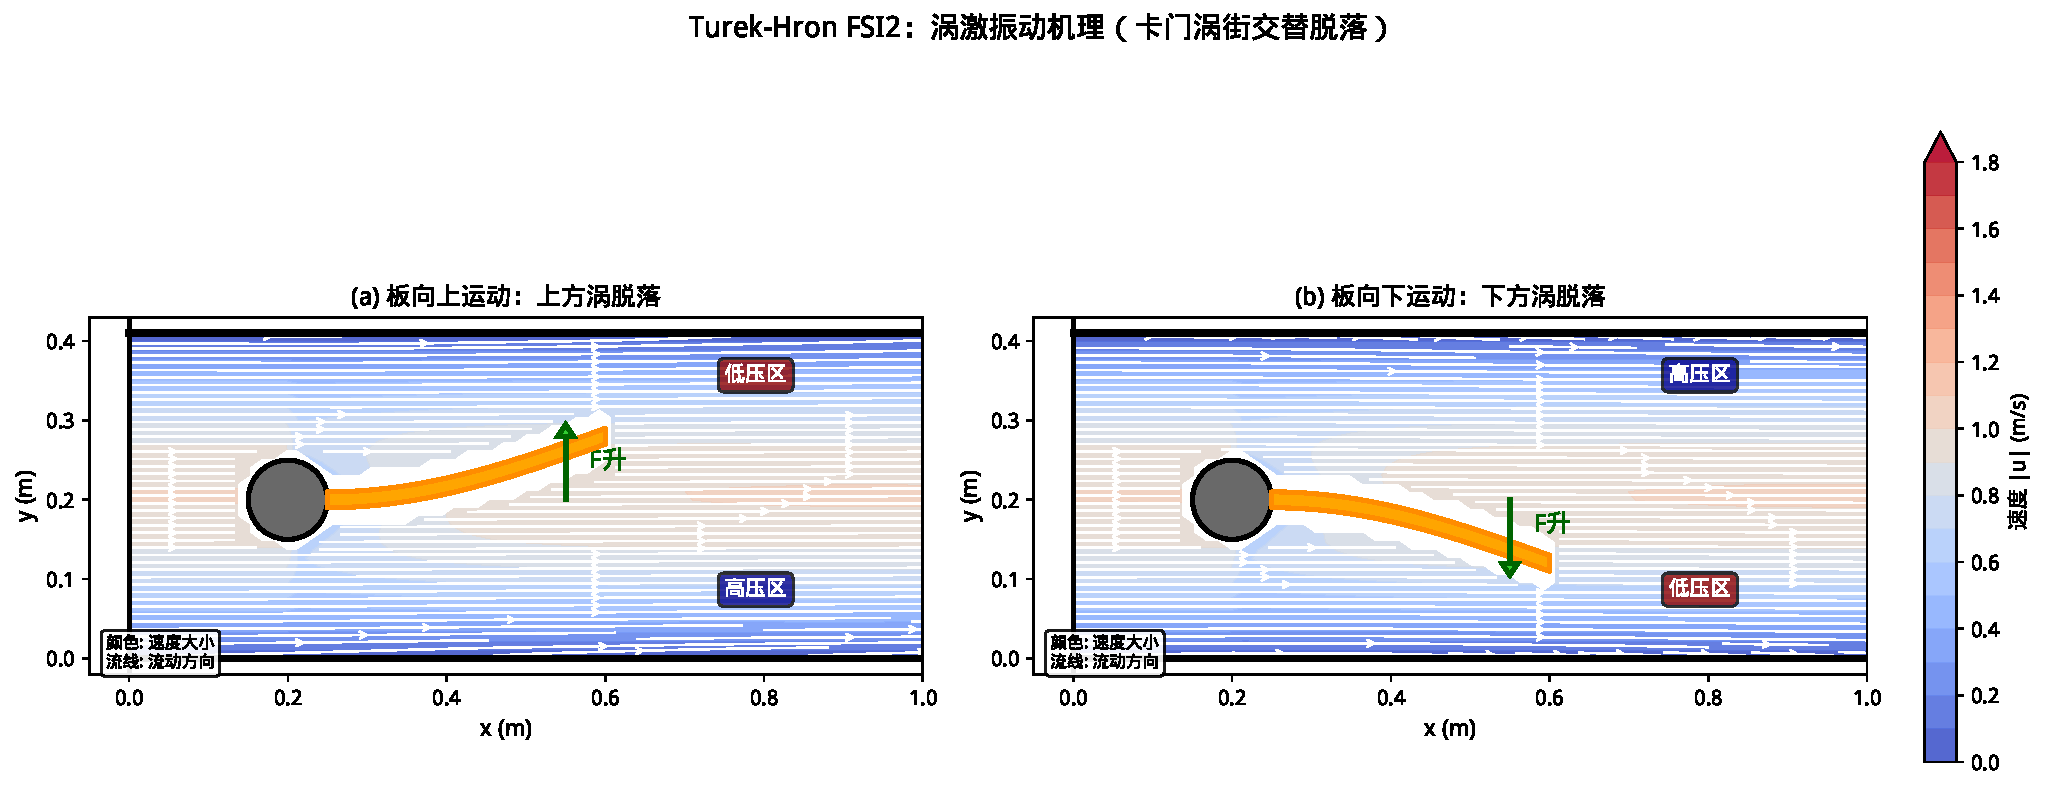
\includegraphics[width=0.98\textwidth]{figs_chap05/turek_fsi2_mechanism.pdf}
\caption{涡激振动机理示意。(a) 当上方涡脱落时，圆柱和板上方形成低压区，产生向上的升力，推动弹性板向上弯曲。(b) 半个周期后，下方涡脱落，下方形成低压区，产生向下的升力。这种交替的压力差驱动板的周期性振荡。}
\label{fig:turek_fsi2_mechanism}
\end{figure}

涡脱落频率由\textbf{Strouhal数}确定：
\begin{equation}
f_s = \text{St} \cdot \frac{U}{D}
\end{equation}
其中$\text{St} \approx 0.2$对于许多钝体都近似成立。对于FSI2条件：$f_s \approx 0.2 \times 1.0 / 0.1 = 2$ Hz。

当这个涡脱落频率接近弹性板的固有频率时，会发生\textbf{锁定}（lock-in）现象：
\begin{itemize}
    \item 涡脱落频率被"锁定"到结构固有频率
    \item 振幅急剧增大
    \item 流固相互作用形成正反馈，系统进入\textbf{自激振荡}
\end{itemize}

% ------------------------------------------------------------------------------------
\subsection*{三、振动响应}

经过初始瞬态后，弹性板进入稳态周期振荡。图\ref{fig:turek_fsi2_snapshots}展示了一个振动周期内弹性板的变形序列。

\begin{figure}[htbp]
\centering
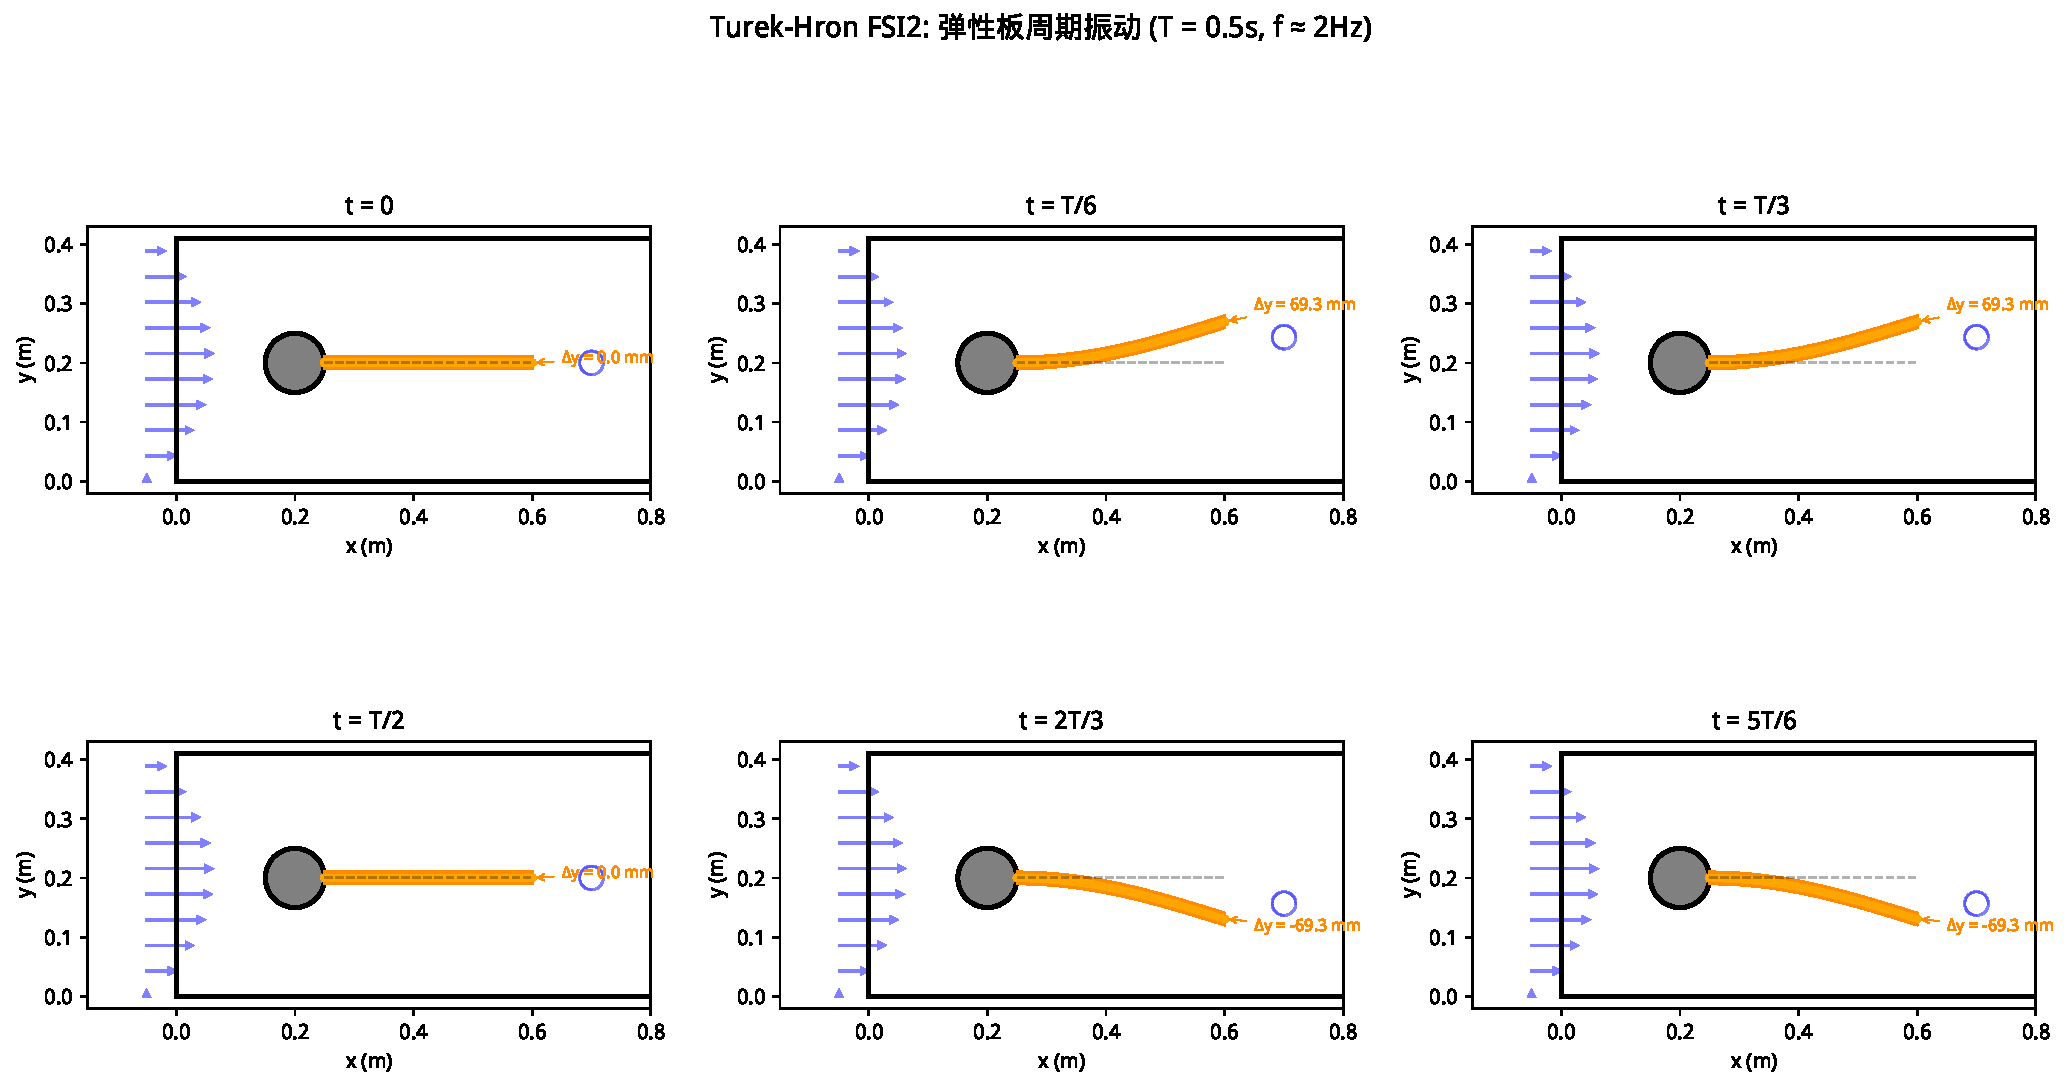
\includegraphics[width=0.98\textwidth]{figs_chap05/turek_fsi2_snapshots.pdf}
\caption{Turek-Hron FSI2：弹性板在一个振动周期（$T \approx 0.5$ s）内的变形快照。板端Y方向位移幅值约$\pm 80$ mm，这是板长（350 mm）的约23\%——属于大变形范畴！注意板的变形主要由一阶弯曲模态主导。}
\label{fig:turek_fsi2_snapshots}
\end{figure}

图\ref{fig:turek_fsi2_analysis}给出了完整的动力学分析。

\begin{figure}[htbp]
\centering
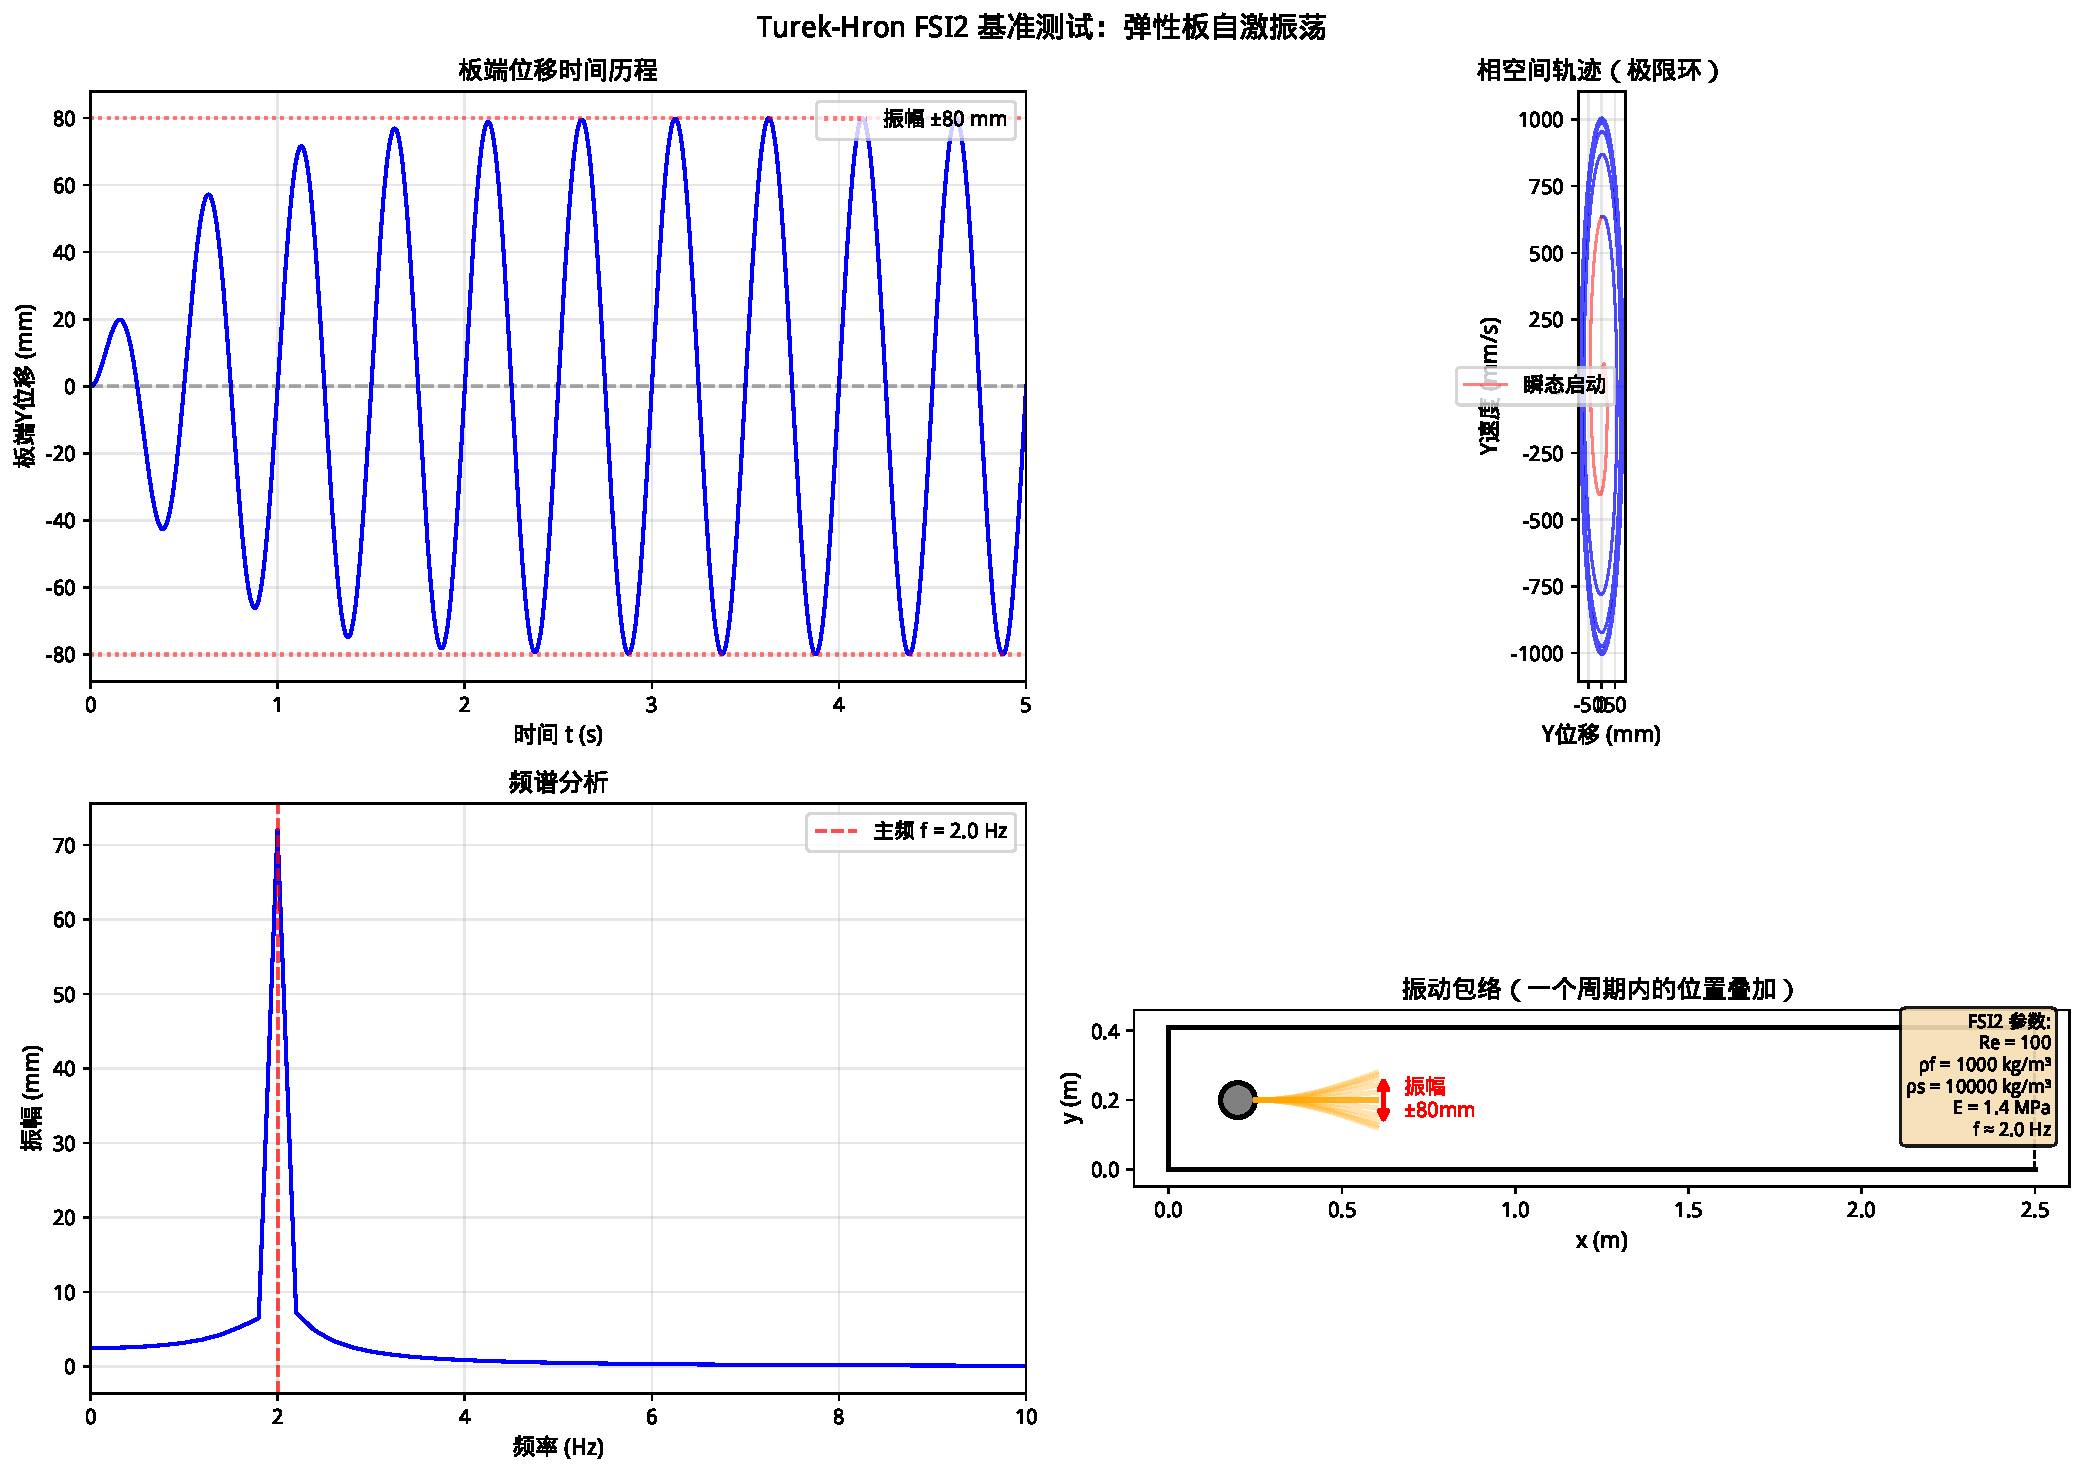
\includegraphics[width=0.98\textwidth]{figs_chap05/turek_fsi2_time_history.pdf}
\caption{Turek-Hron FSI2动力学分析。\textbf{左上}：板端Y位移时间历程——经过短暂瞬态后进入稳态振荡，振幅约$\pm 80$ mm。\textbf{右上}：相空间轨迹——稳态时形成极限环（limit cycle），这是自激振荡的标志。\textbf{左下}：频谱分析——主频约2 Hz，与涡脱落频率一致。\textbf{右下}：振动包络——一个周期内板的位置叠加，展示振动的空间范围。}
\label{fig:turek_fsi2_analysis}
\end{figure}

\paragraph{文献参考值}
Turek和Hron报告的FSI2基准结果：
\begin{itemize}
    \item 板端Y方向位移：$y(A) = 1.23 \pm 80.6 \times 10^{-3}$ m（均值1.23 mm，振幅80.6 mm）
    \item 振动频率：$f \approx 2.0$ Hz
    \item 圆柱阻力系数：$C_D = 208.83 \pm 73.75$
    \item 圆柱升力系数：$C_L = 0.88 \pm 234.2$
\end{itemize}

% ------------------------------------------------------------------------------------
\subsection*{四、结构建模：Euler-Bernoulli梁有限元}

弹性板可以用\textbf{Euler-Bernoulli梁理论}建模。控制方程为：
\begin{equation}
EI \frac{\partial^4 w}{\partial x^4} + \rho A \frac{\partial^2 w}{\partial t^2} = f(x, t)
\end{equation}
其中$w(x,t)$是横向位移，$EI$是抗弯刚度，$\rho A$是单位长度质量，$f(x,t)$是流体力。

\subsubsection*{单元刚度矩阵与质量矩阵}

对于长度为$L_e$的梁单元，每端有两个自由度（位移$w$和转角$\theta$），单元矩阵是$4 \times 4$的：
\begin{equation}
\mathbf{K}_e = \frac{EI}{L_e^3}
\begin{pmatrix}
12 & 6L_e & -12 & 6L_e \\
6L_e & 4L_e^2 & -6L_e & 2L_e^2 \\
-12 & -6L_e & 12 & -6L_e \\
6L_e & 2L_e^2 & -6L_e & 4L_e^2
\end{pmatrix}, \quad
\mathbf{M}_e = \frac{\rho A L_e}{420}
\begin{pmatrix}
156 & 22L_e & 54 & -13L_e \\
22L_e & 4L_e^2 & 13L_e & -3L_e^2 \\
54 & 13L_e & 156 & -22L_e \\
-13L_e & -3L_e^2 & -22L_e & 4L_e^2
\end{pmatrix}
\end{equation}

\begin{marginnote}
\textbf{注意}：FSI2涉及大变形，严格来说需要使用几何非线性公式（如协同旋转法或Total Lagrangian公式）。这里的线性梁模型只是演示目的。
\end{marginnote}

% ------------------------------------------------------------------------------------
\subsection*{五、完整FSI求解的挑战}

Turek-Hron FSI2之所以成为经典基准，是因为它包含了FSI问题的核心难点：

\begin{insightbox}
\textbf{FSI2的挑战}：
\begin{enumerate}
    \item \textbf{大变形}：板端位移约80 mm，是板长的23\%，几何非线性显著
    \item \textbf{强耦合}：密度比$\rho_s/\rho_f = 10$适中，流固相互作用强烈
    \item \textbf{自激振荡}：不是外加强迫振动，而是系统自发产生的不稳定性
    \item \textbf{双向耦合}：结构变形影响流场，流场变化又反馈到结构力
\end{enumerate}
\end{insightbox}

完整求解FSI2需要同时求解：
\begin{itemize}
    \item \textbf{流体}：不可压缩Navier-Stokes方程
    \begin{equation}
    \rho_f \left( \frac{\partial \mathbf{v}}{\partial t} + \mathbf{v} \cdot \nabla \mathbf{v} \right) = -\nabla p + \mu_f \nabla^2 \mathbf{v}
    \end{equation}
    \item \textbf{固体}：非线性弹性动力学方程（Saint-Venant-Kirchhoff材料）
    \item \textbf{耦合条件}：流固界面上速度连续、应力平衡
\end{itemize}

这需要迭代求解或整体求解，计算成本比单独的流体或结构问题高1-2个数量级。

% ------------------------------------------------------------------------------------
\subsection*{六、开源实现}

\begin{marginnote}
\textbf{开源FSI框架}：
\begin{itemize}
    \item \textbf{Kratos Multiphysics}：完整的多物理场框架
    \item \textbf{preCICE}：耦合库，连接不同求解器
    \item \textbf{Feel++}：C++ FEM库
    \item \textbf{oomph-lib}：牛津大学开发的多物理场库
    \item \textbf{OpenFOAM + CalculiX}：流体+结构组合
\end{itemize}
这些都包含Turek-Hron基准案例的实现。
\end{marginnote}

完整的Python可视化代码位于\texttt{code\_chap05/turek\_fsi2\_visualization.py}，用于生成本节的示意图。真正的FSI2求解需要使用专业的多物理场软件。

\begin{lstlisting}[language=Python, caption=弹性板变形计算示意]
def flag_deformation(s, t, amplitude=0.080, freq=2.0):
    """
    计算弹性板在给定时刻的变形
    s: 沿板长度的参数 [0, 1], 0=固定端, 1=自由端
    t: 时间
    """
    # 一阶弯曲模态: phi(s) ~ 1 - cos(pi*s/2)
    phi = 1 - np.cos(np.pi * s / 2)
    omega = 2 * np.pi * freq
    y_displacement = amplitude * phi * np.sin(omega * t)
    return y_displacement
\end{lstlisting}

% ------------------------------------------------------------------------------------
\subsection*{七、工程意义}

涡激振动不仅是学术问题，在工程中有重大实际意义：

\begin{itemize}
    \item \textbf{海洋工程}：深海立管（riser）在洋流中的涡激振动是设计的主要挑战
    \item \textbf{桥梁工程}：塔科马海峡大桥（1940年坍塌）的前期振动就与涡激振动有关
    \item \textbf{航空航天}：飞机机翼、尾翼的气动弹性颤振
    \item \textbf{能源工程}：风力机叶片、热交换器管束的振动
\end{itemize}

\begin{marginnote}
\textbf{塔科马海峡大桥}（1940年坍塌）长期被误解为共振导致。现代分析表明，真正原因是\textbf{气动弹性颤振}——一种更复杂的流固耦合不稳定性。但涡激振动确实是该桥在坍塌前频繁振动的重要原因。
\end{marginnote}

如果你的FSI代码能正确重现Turek-Hron基准的结果，那它就有了一定的可信度。这就是为什么FSI2成为了验证FSI求解器的"金标准"。

\begin{references}
\bibitem{turek2006proposal} S. Turek and J. Hron, ``Proposal for Numerical Benchmarking of Fluid-Structure Interaction between an Elastic Object and Laminar Incompressible Flow,'' in \textit{Fluid-Structure Interaction}, Lecture Notes in Computational Science and Engineering, vol. 53, Springer, 2006, pp. 371--385.
\end{references}

\begin{figure}[htbp]
\centering
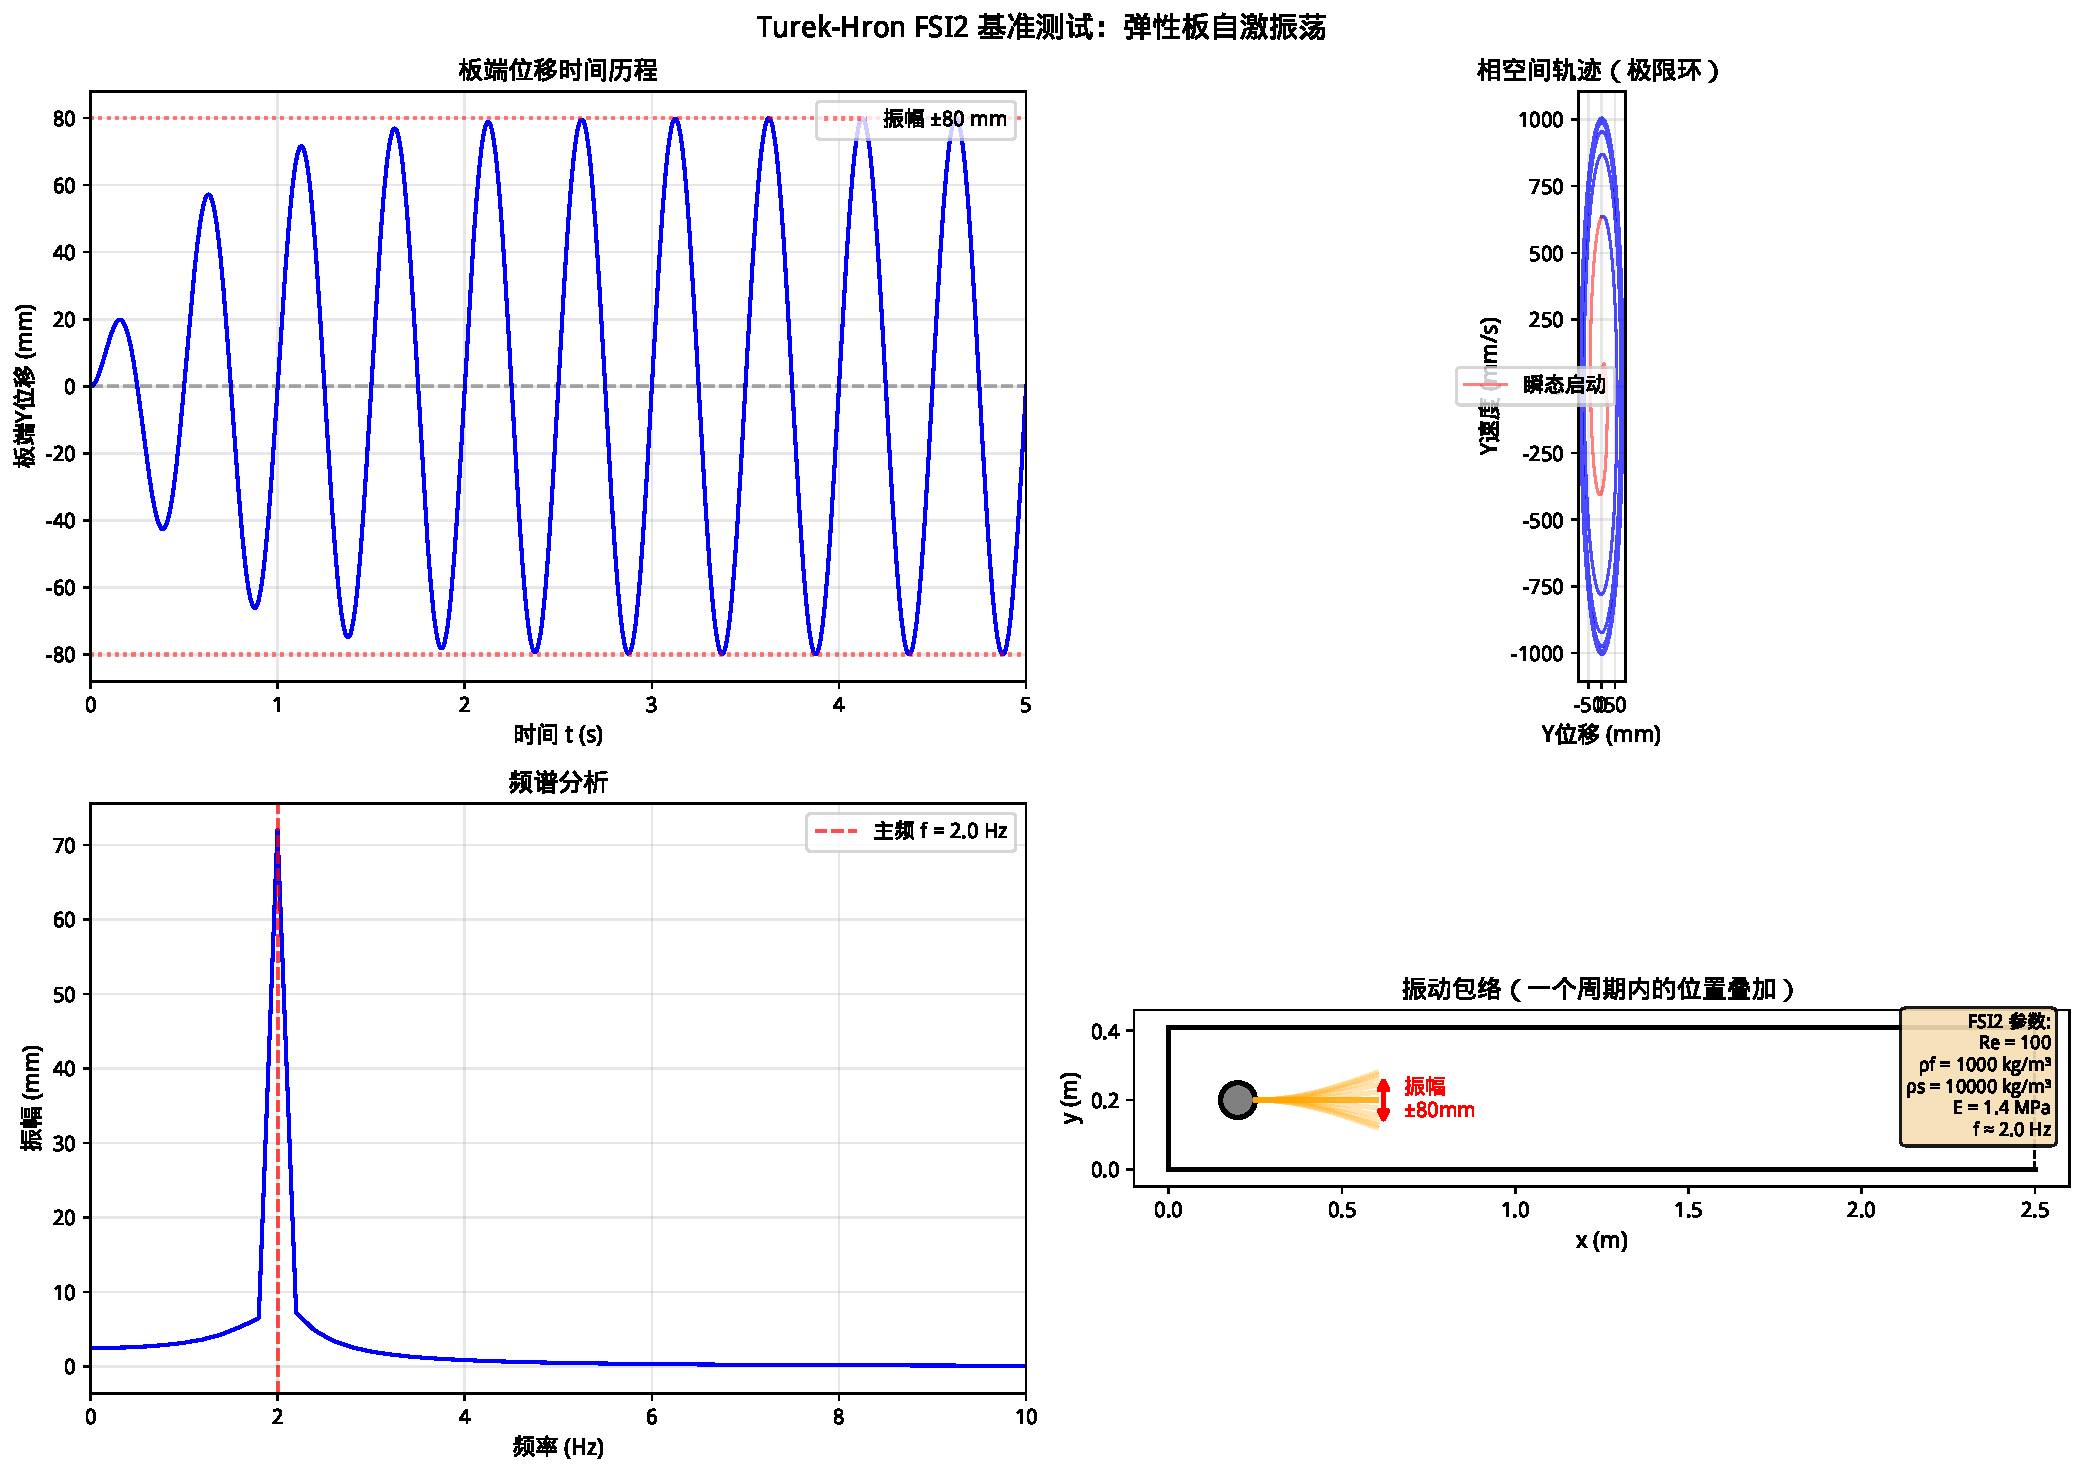
\includegraphics[width=0.98\textwidth]{figs_chap05/turek_fsi2_time_history.pdf}
\caption{Turek-Hron FSI2动力学分析。\textbf{左上}：板端Y位移时间历程，经过短暂瞬态后进入稳态振荡。\textbf{右上}：相空间轨迹，稳态时形成极限环（limit cycle）。\textbf{左下}：频谱分析显示主频约2 Hz。\textbf{右下}：振动包络展示一个周期内板的位置叠加。}
\label{fig:turek_fsi2_analysis}
\end{figure}

\paragraph{涡激振动机理}
为什么弹性板会自发振荡？图\ref{fig:turek_fsi2_mechanism}解释了涡激振动的物理机理：

\begin{figure}[htbp]
\centering
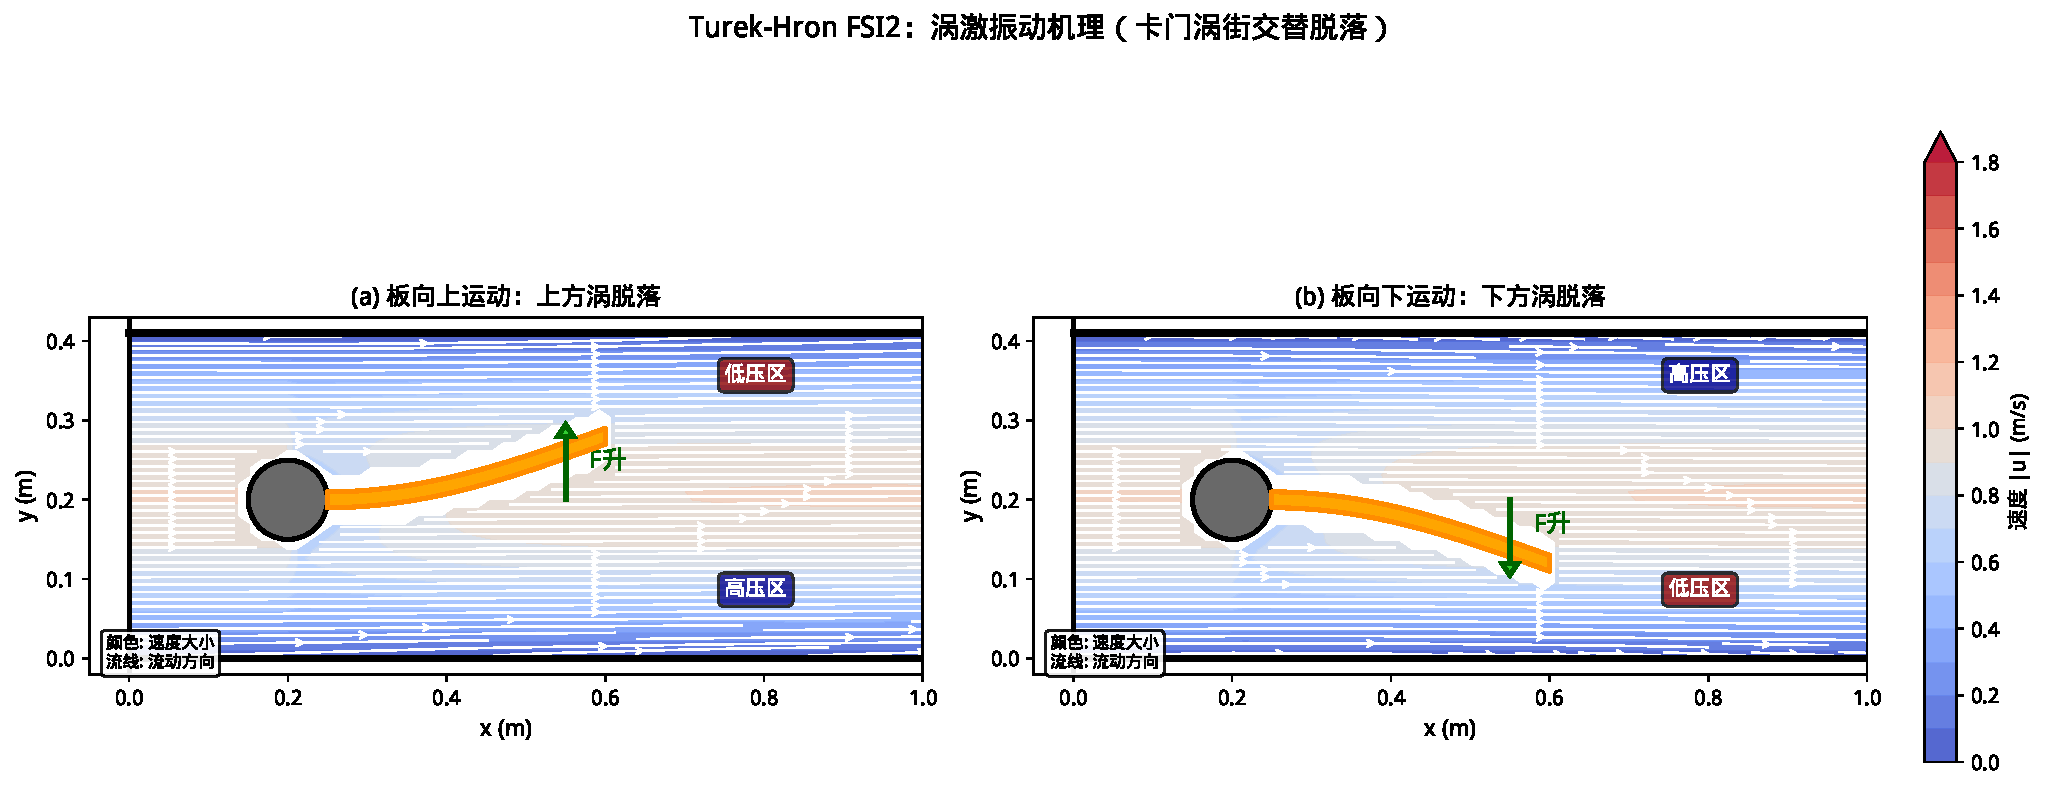
\includegraphics[width=0.98\textwidth]{figs_chap05/turek_fsi2_mechanism.pdf}
\caption{涡激振动机理示意。流体绕过圆柱时形成交替脱落的卡门涡街。(a) 当上方涡脱落时，上方形成低压区，产生向上的升力，推动板向上弯曲。(b) 半个周期后，下方涡脱落，下方形成低压区，产生向下的升力。这种交替的压力差驱动板的周期性振荡。当涡脱落频率接近板的固有频率时，发生\textbf{锁定}（lock-in），振幅达到最大。}
\label{fig:turek_fsi2_mechanism}
\end{figure}

\begin{insightbox}
\textbf{为什么Turek-Hron基准如此重要？}

\begin{enumerate}
    \item \textbf{大变形}：板的位移幅度与板长相当，几何非线性显著
    \item \textbf{强耦合}：固液密度比适中（$\rho_s/\rho_f = 10$），流固相互作用强烈
    \item \textbf{自激振荡}：不是外加强迫振动，而是系统自发产生的不稳定性
    \item \textbf{无实验噪声}：作为数值基准，可以进行严格的代码间比较
\end{enumerate}

如果你的FSI代码能正确重现Turek-Hron基准的结果，那它就有了一定的可信度。
\end{insightbox}

\begin{marginnote}
\textbf{开源实现}：许多开源FSI框架都包含Turek-Hron基准案例，包括：
\begin{itemize}
    \item Kratos Multiphysics
    \item preCICE（耦合库）
    \item Feel++
    \item oomph-lib
\end{itemize}
这些都是学习完整FSI仿真的好资源。
\end{marginnote}

\paragraph{与本节模型的对比}
本节前面的悬臂梁模型（单向耦合、小变形）与Turek-Hron问题（双向耦合、大变形）有本质区别：

\begin{center}
\renewcommand{\arraystretch}{1.3}
\begin{tabular}{l|c|c}
\toprule
& \textbf{本节简化模型} & \textbf{Turek-Hron FSI2} \\
\midrule
流固耦合 & 单向（流$\to$固） & 双向（流$\leftrightarrow$固） \\
变形量级 & 小变形（$w \ll L$） & 大变形（$w \sim L$） \\
流动建模 & 经验公式（Strouhal） & 完整Navier-Stokes \\
计算成本 & 秒级 & 小时/天级 \\
适用场景 & 工程估算、物理直觉 & 精确预测、代码验证 \\
\bottomrule
\end{tabular}
\end{center}

从简化模型到完整的双向耦合FSI，是计算成本增加几个数量级的跨越。但两者并非互斥——简化模型帮助我们建立物理直觉，完整模型用于精确预测和验证。

\begin{references}
\bibitem{turek2006proposal} S. Turek and J. Hron, ``Proposal for Numerical Benchmarking of Fluid-Structure Interaction between an Elastic Object and Laminar Incompressible Flow,'' in \textit{Fluid-Structure Interaction}, Lecture Notes in Computational Science and Engineering, vol. 53, Springer, 2006, pp. 371--385.
\end{references}

  % 第5章：有限元方法

% ####################################################################################
%                              第三部分：控制与信息
% ####################################################################################

\part{控制、信息与机器人}

% ====================================================================================
\chapter{机器人运动学与动力学}
% ====================================================================================

\section*{让机器动起来}

\storynote{Marc Raibert}{Boston Dynamics 创始人（1949--）。1980 年代他在 MIT 造出第一台单腿跳跃机器人，靠三条简单的控制律就让它站稳；后来的 BigDog、Atlas 都是这条路的延续。他的口头禅：“先让它跳起来，再想怎么落地。”}

\vspace{0.5cm}
\noindent\textit{你的手臂有7个自由度，但你从来不需要“计算”如何拿起一杯咖啡。机器人却需要——它必须把“拿杯子”这个任务翻译成每个关节应该转多少度。}

试着做一个实验：伸出你的手，保持手掌位置不动，然后移动你的手肘。你会发现，即使手掌固定，手肘仍然可以在一个圆弧上运动。这说明什么？你的手臂有“多余”的自由度——完成“固定手掌”这个任务后，还剩下一些自由度可以用来做别的事情。

这个简单的观察背后，是机器人学中一个核心问题：\textbf{运动学}——关节角度和末端位置之间的关系。更深一层，当机器人需要推、拉、抓取物体时，我们还需要\textbf{动力学}——力、质量、加速度之间的关系。

本章将展示：第5章学到的拉格朗日力学如何直接应用于机器人。你会发现，末端约束力、接触力都是拉格朗日乘子的工程化身，而关节力矩通过 $\tau = J^\top F$ 与它们相连。

\begin{quote}
\textbf{本章目标}：机器人是拉格朗日力学最直接的工程应用——把末端“钉”在目标上的约束力、脚与地面之间的接触力，都是第1章的拉格朗日乘子，只是这一次它们是真真切切的牛顿。本章将建立从“任务描述”到“关节力矩”的完整链条。
\end{quote}

\begin{tcolorbox}[colback=green!5, colframe=green!60!black, title=学完这章，你将能够...]
\begin{itemize}
    \item 用齐次变换建立机械臂的正运动学模型（D-H 参数是它的标准化写法）
    \item 计算雅可比矩阵，分析奇异构型
    \item 求解简单机械臂的逆运动学（解析解或数值解）
    \item 用拉格朗日方法推导机器人动力学方程
    \item 理解关节力矩与末端力的映射关系
\end{itemize}
\end{tcolorbox}

% ------------------------------------------------------------------------------------
\section{从人手臂到机械臂}

\subsection{为什么机器人需要“算”？}

人类拿起一杯咖啡，大脑只需要想“拿杯子”，手臂就自动完成了。我们从不需要计算“肩关节转23度，肘关节转45度，腕关节转-12度”。这件事在人看来毫不费力，对机器却出奇地难：1980 年代 Hans Moravec 就指出，让计算机下棋容易，让它像一岁小孩那样感知和运动却极难——这就是后来所说的莫拉维克悖论。

机器人的“大脑”（控制器）收到的命令是“把末端移动到坐标(0.5, 0.3, 0.2)”，它必须计算出每个电机应该转多少度。这个过程叫做\textbf{逆运动学}。1961 年，第一台工业机器人 Unimate 已经在通用汽车的生产线上搬运压铸件——从那时起，“把任务翻译成关节角”就是每一台机械臂绕不开的问题。

反过来，如果我们知道每个关节的角度，要算出末端在哪里，这叫做\textbf{正运动学}。正运动学相对简单——就是一连串的几何变换。逆运动学则困难得多——它可能有多个解，也可能无解。

\begin{figure}[htbp]
\centering
\begin{tikzpicture}[scale=1.0]
    % 左边：关节空间
    \begin{scope}[shift={(-4,0)}]
        \node[draw, rounded corners, fill=blue!10, minimum width=3cm, minimum height=2cm] (joint) at (0,0) {
            \begin{tabular}{c}
            \textbf{关节空间} \\
            $q = (q_1, q_2, \ldots, q_n)$ \\
            \small 每个关节转多少度？
            \end{tabular}
        };
    \end{scope}
    
    % 右边：任务空间
    \begin{scope}[shift={(4,0)}]
        \node[draw, rounded corners, fill=red!10, minimum width=3cm, minimum height=2cm] (task) at (0,0) {
            \begin{tabular}{c}
            \textbf{任务空间} \\
            $x = (\text{位置, 姿态})$ \\
            \small 末端在哪里？朝哪？
            \end{tabular}
        };
    \end{scope}
    
    % 箭头
    \draw[->, thick, blue] (joint.east) -- (task.west) 
        node[midway, above] {正运动学 $x = f(q)$}
        node[midway, below] {\small 简单、唯一};
    \draw[->, thick, red, transform canvas={yshift=-1.5cm}] (task.west) -- (joint.east) 
        node[midway, above] {逆运动学 $q = f^{-1}(x)$}
        node[midway, below] {\small 困难、可能多解};
\end{tikzpicture}
\caption{机器人的两种“语言”：关节空间与任务空间}
\end{figure}

\subsection{自由度的概念}

\textbf{自由度}（Degrees of Freedom, DoF）是描述系统需要多少个独立参数才能完全确定其位置。

\begin{example}[日常生活中的自由度]
一扇门只能绕铰链转动，一个抽屉只能前后滑动，它们都只有 1 个自由度；一把办公椅可以上下、前后、旋转、靠背倾斜，自由度有 5--6 个；人的手臂有 7 个自由度（肩 3 个、肘 1 个、腕 3 个），而每根手指也有大约 4 个。
\end{example}

\sidenoteplain{为什么人的手臂是7个自由度而不是6个？因为我们需要在固定手掌位置的同时，还能调整手肘位置（比如绕开障碍物）。这个“多出来”的自由度叫做\textbf{冗余自由度}。}

任务空间通常是6维的：3个位置 $(x, y, z)$ + 3个姿态（如欧拉角或四元数的3个独立分量）。

\begin{center}
\renewcommand{\arraystretch}{1.3}
\small
\begin{tabularx}{\linewidth}{l|c|c|X}
\toprule
\textbf{机械臂类型} & \textbf{关节数 $n$} & \textbf{与任务空间比较} & \textbf{特点} \\
\midrule
SCARA（平面装配） & 4 & $n < 6$ & 姿态受限：末端只能绕竖直轴转动 \\
典型工业臂 & 6 & $n = 6$ & 恰好完成6D任务 \\
人形机械臂 & 7 & $n > 6$ & 冗余，更灵活 \\
双臂机器人 & 14 & $n \gg 6$ & 高度冗余 \\
\bottomrule
\end{tabularx}
\end{center}

% ------------------------------------------------------------------------------------
\section{运动学基础}

\subsection{齐次变换：旋转与平移的统一表示}

描述物体在三维空间中的位置和姿态，需要同时处理旋转和平移。\textbf{齐次变换矩阵}把这两者统一成一个 $4 \times 4$ 矩阵：

\begin{definition}[齐次变换]
\begin{equation}
T = \begin{bmatrix} R & p \\ 0 & 1 \end{bmatrix} \in SE(3)
\end{equation}
其中 $R \in SO(3)$ 是 $3 \times 3$ 旋转矩阵，$p \in \mathbb{R}^3$ 是平移向量。
\end{definition}

齐次变换的美妙之处在于：\textbf{多次变换可以通过矩阵乘法串联}。
\preview{$SO(3)$、$SE(3)$ 是“所有旋转矩阵”和“所有位姿”这两个集合的名字。旋转矩阵有 9 个数，为什么只有 3 个自由度？本章末尾的扩展阅读会用拉格朗日乘子法回答。}

\begin{example}[两次变换的串联]
假设坐标系A相对于世界坐标系的变换是 $T_A$，坐标系B相对于A的变换是 $T_B$，那么B相对于世界坐标系的变换是：
\[
T_{world \to B} = T_A \cdot T_B
\]
就这么简单！矩阵乘法帮我们处理了所有复杂的几何关系。
\end{example}

\subsection{正运动学：从关节到末端}

对于 $n$ 关节的机械臂，每个关节 $i$ 贡献一个变换 $T_i(q_i)$（取决于关节角 $q_i$）。末端相对于基座的变换是所有关节变换的乘积：

\begin{equation}
T_{end}(q) = T_1(q_1) \cdot T_2(q_2) \cdots T_n(q_n)
\end{equation}

\begin{example}[平面双连杆机械臂的正运动学]
考虑最简单的情况：两个连杆在平面内运动，长度分别为 $L_1$ 和 $L_2$。
\sidenoteplain{\textbf{D-H参数}：机器人运动学的标准表示法由Jacques Denavit和Richard Hartenberg于1955年提出。这套参数用4个数描述每个关节，使得任何串联机械臂都能用统一的框架分析。几乎所有工业机器人的技术手册都使用D-H参数。}

\begin{figure}[htbp]
\centering
\begin{tikzpicture}[scale=1.5]
    % 坐标系
    \draw[->] (-0.5,0) -- (3,0) node[right] {$x$};
    \draw[->] (0,-0.5) -- (0,2) node[above] {$y$};
    
    % 连杆1
    \draw[very thick, blue] (0,0) -- ({1.5*cos(50)},{1.5*sin(50)});
    \node[blue, above left] at ({0.75*cos(50)},{0.75*sin(50)}) {$L_1$};
    
    % 连杆2
    \draw[very thick, red] ({1.5*cos(50)},{1.5*sin(50)}) -- 
        ({1.5*cos(50)+1.2*cos(50-30)},{1.5*sin(50)+1.2*sin(50-30)});
    \node[red, above right] at ({1.5*cos(50)+0.6*cos(50-30)},{1.5*sin(50)+0.6*sin(50-30)}) {$L_2$};
    
    % 关节
    \fill (0,0) circle (2pt);
    \fill ({1.5*cos(50)},{1.5*sin(50)}) circle (2pt);
    \fill ({1.5*cos(50)+1.2*cos(50-30)},{1.5*sin(50)+1.2*sin(50-30)}) circle (3pt);
    \node[right] at ({1.5*cos(50)+1.2*cos(50-30)},{1.5*sin(50)+1.2*sin(50-30)}) {末端 $(x,y)$};
    
    % 角度
    \draw[->] (0.5,0) arc (0:50:0.5);
    \node at (0.7,0.3) {$q_1$};
    
    \draw[->] ({1.5*cos(50)+0.4*cos(50)},{1.5*sin(50)+0.4*sin(50)}) 
        arc (50:20:0.4);
    \node at ({1.5*cos(50)+0.5},{1.5*sin(50)+0.1}) {$q_2$};
\end{tikzpicture}
\caption{平面双连杆机械臂}
\end{figure}

正运动学方程：
\begin{align}
x &= L_1 \cos q_1 + L_2 \cos(q_1 + q_2) \\
y &= L_1 \sin q_1 + L_2 \sin(q_1 + q_2)
\end{align}

这个公式很直观：第一项 $(L_1 \cos q_1, L_1 \sin q_1)$ 是肘关节的位置，第二项是从肘关节到末端的位移，它的方向是 $q_1 + q_2$——第二根连杆的绝对转角是两个关节角之和。
\end{example}

\begin{example}[手算练习]
设 $L_1 = L_2 = 1$，$q_1 = 60°$，$q_2 = -30°$，求末端位置。

\textbf{解}：
\begin{align}
x &= \cos 60° + \cos(60° - 30°) = 0.5 + \cos 30° = 0.5 + 0.866 = 1.366 \\
y &= \sin 60° + \sin 30° = 0.866 + 0.5 = 1.366
\end{align}

末端位置约为 $(1.37, 1.37)$。
\end{example}

% ------------------------------------------------------------------------------------
\section{雅可比矩阵：连接速度与力的桥梁}

\subsection{为什么需要雅可比？}

正运动学告诉我们“位置”的关系：$x = f(q)$。但在控制中，我们经常需要知道“速度”的关系：关节转得多快，末端就移动得多快？

这就是\textbf{雅可比矩阵}的作用——它是 $f(q)$ 的一阶导数，描述速度的映射关系。

\begin{definition}[雅可比矩阵]
末端速度与关节速度的关系：
\begin{equation}
\dot{x} = J(q) \dot{q}
\end{equation}
其中 $J(q) = \frac{\partial f}{\partial q}$ 是 $m \times n$ 的雅可比矩阵（$m$是任务空间维度，$n$是关节数）。
\end{definition}

\begin{example}[双连杆机械臂的雅可比]
对正运动学方程求导：
\begin{equation}
J = \begin{bmatrix} 
\frac{\partial x}{\partial q_1} & \frac{\partial x}{\partial q_2} \\[6pt]
\frac{\partial y}{\partial q_1} & \frac{\partial y}{\partial q_2}
\end{bmatrix}
= \begin{bmatrix}
-L_1 \sin q_1 - L_2 \sin(q_1+q_2) & -L_2 \sin(q_1+q_2) \\
L_1 \cos q_1 + L_2 \cos(q_1+q_2) & L_2 \cos(q_1+q_2)
\end{bmatrix}
\end{equation}

注意 $J$ 依赖于当前位形 $q$——机械臂在不同姿态下，速度传递关系是不同的。
\end{example}

\subsection{力的对偶关系：雅可比的转置}

雅可比矩阵有一个神奇的性质：它的\textbf{转置}把末端力映射到关节力矩。

\begin{keytheorem}[title=力/力矩转换]
\begin{equation}
\boxed{\tau = J(q)^\top F}
\end{equation}
末端力 $F \in \mathbb{R}^m$ 需要关节力矩 $\tau \in \mathbb{R}^n$ 来平衡。
\end{keytheorem}

\begin{physicalmeaning}
这个公式来自\textbf{虚功原理}——关节空间做的虚功必须等于任务空间做的虚功：
\[
\delta W = \tau^\top \delta q = F^\top \delta x = F^\top J \delta q
\]
由于 $\delta q$ 是任意的，必有 $\tau = J^\top F$。

\textbf{直觉}：$J$ 把关节速度“放大”成末端速度，$J^\top$ 把末端力“缩小”成关节力矩。速度放大多少倍，力就缩小多少倍——这是杠杆原理的推广！
\end{physicalmeaning}
\review{第5章}{第5章把“力”推广成了广义力——作用在广义坐标 $q_i$ 方向上的力。$\tau = J^\top F$ 正是这个推广：末端力 $F$ 投影到每个关节角方向，就是那个关节要出的力矩。}

\begin{example}[力的传递]
双连杆机械臂，$L_1 = L_2 = 1$m，$q_1 = 90°$，$q_2 = 0°$（手臂竖直向上伸直）。

末端受到水平向右的力 $F = (10, 0)^\top$ N，求所需的关节力矩。

\textbf{解}：首先计算雅可比：
\[
J = \begin{bmatrix}
-\sin 90° - \sin 90° & -\sin 90° \\
\cos 90° + \cos 90° & \cos 90°
\end{bmatrix}
= \begin{bmatrix}
-2 & -1 \\
0 & 0
\end{bmatrix}
\]

然后：
\[
\tau = J^\top F = \begin{bmatrix} -2 & 0 \\ -1 & 0 \end{bmatrix} \begin{bmatrix} 10 \\ 0 \end{bmatrix}
= \begin{bmatrix} -20 \\ -10 \end{bmatrix} \text{ Nm}
\]

\textbf{物理解释}：要抵抗水平向右的力，两个关节都需要产生负的（顺时针）力矩。肩关节力矩是肘关节的两倍，因为它到末端的力臂更长。
\end{example}

\subsection{奇异性：机械臂的“盲区”}

当雅可比矩阵不满秩时（$\det(J) = 0$ 对于方阵，或 $\text{rank}(J) < \min(m,n)$），机械臂处于\textbf{奇异位形}。

\begin{figure}[htbp]
\centering
\begin{tikzpicture}[scale=1.0]
    % 正常位形
    \begin{scope}[shift={(0,0)}]
        \draw[very thick, blue] (0,0) -- (1.5,1.2);
        \draw[very thick, red] (1.5,1.2) -- (3,0.3);
        \fill (0,0) circle (3pt);
        \fill (1.5,1.2) circle (3pt);
        \fill (3,0.3) circle (3pt);
        
        % 可达方向
        \draw[->, thick, green!60!black] (3,0.3) -- (3.7,0.8);
        \draw[->, thick, green!60!black] (3,0.3) -- (3.7,-0.2);
        \draw[->, thick, green!60!black] (3,0.3) -- (2.3,0.8);
        \node at (3.9,0.3) {\small 全方向可达};
        
        \node[below] at (1.5,-0.3) {\small 正常位形};
    \end{scope}
    
    % 奇异位形
    \begin{scope}[shift={(6,0)}]
        \draw[very thick, blue] (0,0) -- (1.5,0);
        \draw[very thick, red] (1.5,0) -- (3,0);
        \fill (0,0) circle (3pt);
        \fill (1.5,0) circle (3pt);
        \fill (3,0) circle (3pt);
        
        % 可达方向
        \draw[->, thick, green!60!black] (3,0) -- (3,0.7);
        \draw[->, thick, green!60!black] (3,0) -- (3,-0.7);
        \node[above] at (3,0.8) {\small 只能上下};
        
        % 不可达
        \draw[dashed, red] (3,0) -- (3.7,0);
        \node[red, right] at (3.7,0) {\small 无法移动};
        
        \node[below] at (1.5,-0.3) {\small 奇异位形（伸直）};
    \end{scope}
\end{tikzpicture}
\caption{奇异位形：手臂完全伸直时，末端无法沿手臂方向移动}
\end{figure}

奇异性带来两个问题，它们是同一件事的两面。从速度看，$J$ 的列张不满整个任务空间，于是某些方向的末端速度无法通过任何关节速度实现；从力看，由 $\tau = J^\top F$，沿奇异方向的末端力被 $J^\top$ 映射成零，于是无论关节力矩多大，都无法在末端产生这个方向的力。反过来说，手臂伸直时靠结构就能承受这个方向的载荷，不需要力矩。

\begin{example}[伸直位形的奇异性]
当 $q_2 = 0$（手臂伸直）时：
\[
\det(J) = L_1 L_2 \sin q_2 = 0
\]

此时，两个连杆在一条直线上，末端无法沿这条直线方向移动——两个关节的转动都只能让末端垂直于手臂运动。

\textbf{生活类比}：当你的手臂完全伸直时，很难通过弯曲/伸展来让指尖向前移动。你必须先把手肘弯曲一点，才能向前够东西。
\end{example}

% ------------------------------------------------------------------------------------
\section{本章的核心观点}

在动手算逆运动学之前，先把本章放回全书的主线上。

\begin{tcolorbox}[colback=yellow!10, colframe=orange!80, title=核心观点]
\textbf{机器人学没有新的数学——它就是第1章的拉格朗日乘子法，只不过变量是关节角 $q$，约束是“末端要到某处”或“脚不能穿过地面”，而乘子 $\lambda$ 不再是抽象的“价格”，而是真真切切的力。}

约束是什么？——任务（$f(q) = x_d$）和物理（$\phi(q) \ge 0$）。

乘子是什么？——维持这些约束所需要的力：末端约束力、地面反作用力。它们不是从天上掉下来的，而是从一阶条件里自然涌现的。
\end{tcolorbox}

\begin{center}
\renewcommand{\arraystretch}{1.4}
\small
\begin{tabularx}{\linewidth}{l>{\hsize=.62\hsize}X>{\hsize=1.38\hsize}X}
\toprule
 & \textbf{第1章（约束优化）} & \textbf{本章（机器人）} \\
\midrule
变量 & $x \in \R^n$ & 关节角 $q \in \R^n$（动力学中还有 $\ddot{q}$） \\
目标 & $\min f(x)$ & 逆运动学：$\min \tfrac{1}{2}\|q - q_0\|^2$\newline 动力学：作用量 $\int (T - V)\,dt$ \\
等式约束 & $g(x) = 0$ & 末端到达 $f(q) - x_d = 0$\newline 接触保持 $J_c \ddot{q} + \dot{J}_c \dot{q} = 0$ \\
不等式约束 & $h(x) \le 0$ & 不穿透 $-\phi(q) \le 0$\newline 摩擦锥 $\|f_t\| - \mu \lambda_n \le 0$ \\
乘子 & $\lambda$，$\mu \ge 0$ & 末端约束力 $\lambda$；接触力 $\lambda_c$，法向 $\lambda_n \ge 0$ \\
一阶条件 & $\nabla f + \lambda \nabla g = 0$ & $(q - q_0) + J^\top \lambda = 0$\newline $M\ddot{q} + C\dot{q} + G = \tau + J_c^\top \lambda_c$ \\
互补松弛 & $\mu\, h(x) = 0$ & $\lambda_n\, \phi(q) = 0$（悬空无力，接触才有力） \\
影子价格 & $\lambda = -df^*/d\epsilon$ & 目标点移动 $\delta x$，代价变化 $-\lambda^\top \delta x$ \\
\bottomrule
\end{tabularx}
\end{center}

% ------------------------------------------------------------------------------------
\section{逆运动学：约束优化的工程应用}

\subsection{问题的本质}

逆运动学的问题是：给定目标末端位置 $x_d$，求关节角 $q$。

这是一个\textbf{方程求解问题}：
\[
f(q) = x_d
\]

但它经常被转化为\textbf{优化问题}——寻找“最好”的解：

\begin{keyformula}[title=逆运动学的优化形式]
\begin{equation}
\min_q \frac{1}{2}\|q - q_0\|^2 \quad \st \quad f(q) = x_d
\end{equation}

含义：在所有能到达目标的关节角中，选择离当前位置 $q_0$ 最近的。
\end{keyformula}

\begin{physicalmeaning}
为什么要用优化形式？因为方程 $f(q) = x_d$ 本身往往定不下唯一的解：当 $n > m$（冗余机械臂）时它有无穷多解，需要一个选择标准；即使 $n = m$，也可能有多个解（如手肘朝上或朝下），需要选出最自然的那个。写成优化问题之后，这个“选择标准”就是目标函数，而关节限位、避障之类的额外要求也可以作为约束方便地加进来。
\end{physicalmeaning}

\subsection{拉格朗日方法求解}

构造拉格朗日函数：
\begin{equation}
\mathcal{L}(q, \lambda) = \frac{1}{2}\|q - q_0\|^2 + \lambda^\top (f(q) - x_d)
\end{equation}

KKT条件：
\begin{align}
\nabla_q \mathcal{L} &= (q - q_0) + J(q)^\top \lambda = 0 \\
\nabla_\lambda \mathcal{L} &= f(q) - x_d = 0
\end{align}

从第一式解出：
\begin{equation}
q = q_0 - J^\top \lambda
\end{equation}

\begin{physicalmeaning}
$\lambda$ 的物理意义是\textbf{约束力}：如果用一根刚性杆把末端固定在目标位置 $x_d$，需要在末端施加多大的力？

这个力通过 $J^\top$ 传递到关节空间，导致关节偏离“自然位置” $q_0$。
\end{physicalmeaning}
\review{第1章}{影子价格：约束松一点，目标改善多少。这里的约束是 $f(q) = x_d$，把目标点挪动 $\delta x$，代价 $\tfrac{1}{2}\|q - q_0\|^2$ 的变化是 $-\lambda^\top \delta x$——所以 $\lambda$ 的量纲是“力”（能量/位移）。}

\subsection{牛顿迭代法求解逆运动学}

逆运动学方程 $f(q) = x_d$ 是非线性的，没有通用的解析解。我们需要用数值方法。

\paragraph{核心思想：线性化}

回想微积分中的泰勒展开：对于一元函数 $f(x)$，在 $x_0$ 附近：
\[
f(x) \approx f(x_0) + f'(x_0)(x - x_0)
\]

对于向量函数 $f(q)$，类似地：
\[
f(q) \approx f(q_0) + J(q_0)(q - q_0)
\]

其中 $J = \frac{\partial f}{\partial q}$ 就是雅可比矩阵——它是导数在多元情况下的推广。

\paragraph{迭代算法}

既然我们想让 $f(q) = x_d$，把上面的近似代入：
\[
x_d \approx f(q_0) + J(q_0)(q - q_0)
\]

整理得：
\[
q \approx q_0 + J(q_0)^{-1}(x_d - f(q_0))
\]

这给出了一个迭代公式：

\begin{enumerate}
    \item 从初始猜测 $q^{(0)}$ 开始（比如当前关节角度）
    \item 计算当前末端位置：$x^{(k)} = f(q^{(k)})$
    \item 计算误差：$e = x_d - x^{(k)}$（“还差多远”）
    \item 计算雅可比：$J = J(q^{(k)})$
    \item 求解线性方程：$J \cdot \Delta q = e$（“关节要怎么动”）
    \item 更新关节角：$q^{(k+1)} = q^{(k)} + \Delta q$
    \item 如果 $\|e\|$ 足够小，停止；否则回到第2步
\end{enumerate}

\begin{figure}[htbp]
\centering
\begin{tikzpicture}[scale=1.2]
    % 工作空间
    \draw[->] (0,0) -- (4,0) node[right] {$x$};
    \draw[->] (0,0) -- (0,3) node[above] {$y$};
    
    % 目标点
    \fill[red] (3,2) circle (3pt) node[right] {目标 $x_d$};
    
    % 迭代轨迹
    \fill[blue] (1,0.5) circle (2pt) node[below] {$x^{(0)}$};
    \fill[blue] (1.8,1.2) circle (2pt) node[below left] {$x^{(1)}$};
    \fill[blue] (2.5,1.7) circle (2pt) node[below left] {$x^{(2)}$};
    \fill[blue] (2.9,1.95) circle (2pt);
    
    \draw[->, blue, thick] (1,0.5) -- (1.75,1.15);
    \draw[->, blue, thick] (1.8,1.2) -- (2.45,1.65);
    \draw[->, blue, thick] (2.5,1.7) -- (2.85,1.92);
    
    % 说明
    \node at (2,-0.5) {\small 末端位置逐步逼近目标};
\end{tikzpicture}
\caption{牛顿迭代法：每一步都让末端更接近目标}
\end{figure}

\begin{example}[牛顿迭代的手算演示]
双连杆机械臂，$L_1 = L_2 = 1$，目标位置 $x_d = (1.2, 0.9)$。

从初始猜测 $q^{(0)} = (0^\circ, 90^\circ) = (0, 1.571)$ rad 开始（手臂先伸平、再把小臂竖起来）。

\textbf{第一次迭代}：

1. 计算当前末端位置：
\begin{align}
x^{(0)} &= \cos(0^\circ) + \cos(90^\circ) = 1 + 0 = 1 \\
y^{(0)} &= \sin(0^\circ) + \sin(90^\circ) = 0 + 1 = 1
\end{align}

2. 计算误差：
\[
e = x_d - x^{(0)} = (1.2, 0.9) - (1, 1) = (0.2, -0.1)
\]

3. 计算雅可比（代入 $q_1 = 0^\circ$，$q_2 = 90^\circ$）：
\[
J = \begin{bmatrix}
-\sin 0^\circ - \sin 90^\circ & -\sin 90^\circ \\
\cos 0^\circ + \cos 90^\circ & \cos 90^\circ
\end{bmatrix}
= \begin{bmatrix}
-1 & -1 \\
1 & 0
\end{bmatrix}, \qquad \det J = 1
\]

4. 求解 $J \Delta q = e$：
\[
\Delta q = J^{-1} e = \begin{bmatrix} 0 & 1 \\ -1 & -1 \end{bmatrix} \begin{bmatrix} 0.2 \\ -0.1 \end{bmatrix} = (-0.1, -0.1) \text{ rad} = (-5.7^\circ, -5.7^\circ)
\]

5. 更新：
\[
q^{(1)} = q^{(0)} + \Delta q = (-5.7^\circ, 84.3^\circ)
\]

\textbf{检验}：$q^{(1)}$ 对应的末端位置是 $x = \cos(-5.7^\circ) + \cos(78.6^\circ) \approx 1.193$，$y = \sin(-5.7^\circ) + \sin(78.6^\circ) \approx 0.881$，误差已从 $0.22$ 缩小到约 $0.02$。再迭代一两次，就收敛到精确解 $(-4.5^\circ, 82.8^\circ)$（用余弦定理可以验证：$\cos q_2 = (1.2^2 + 0.9^2 - 2)/2 = 0.125$）。

\textbf{关键观察}：每次迭代都在解一个\textbf{线性}方程组 $J \Delta q = e$。非线性问题被分解成了一系列线性问题！
\tryit{换一个初值 $q^{(0)} = (30^\circ, 30^\circ)$ 再算一遍，你会发现第一步 $\Delta q \approx (-55.8^\circ, 98.9^\circ)$——跨度很大，末端反而离目标更远。牛顿法只在解附近才是“二次收敛”的，初值很重要。}
\end{example}

% 代码演示结果（code/chap06_robotics.py）
\begin{figure}[htbp]
\centering
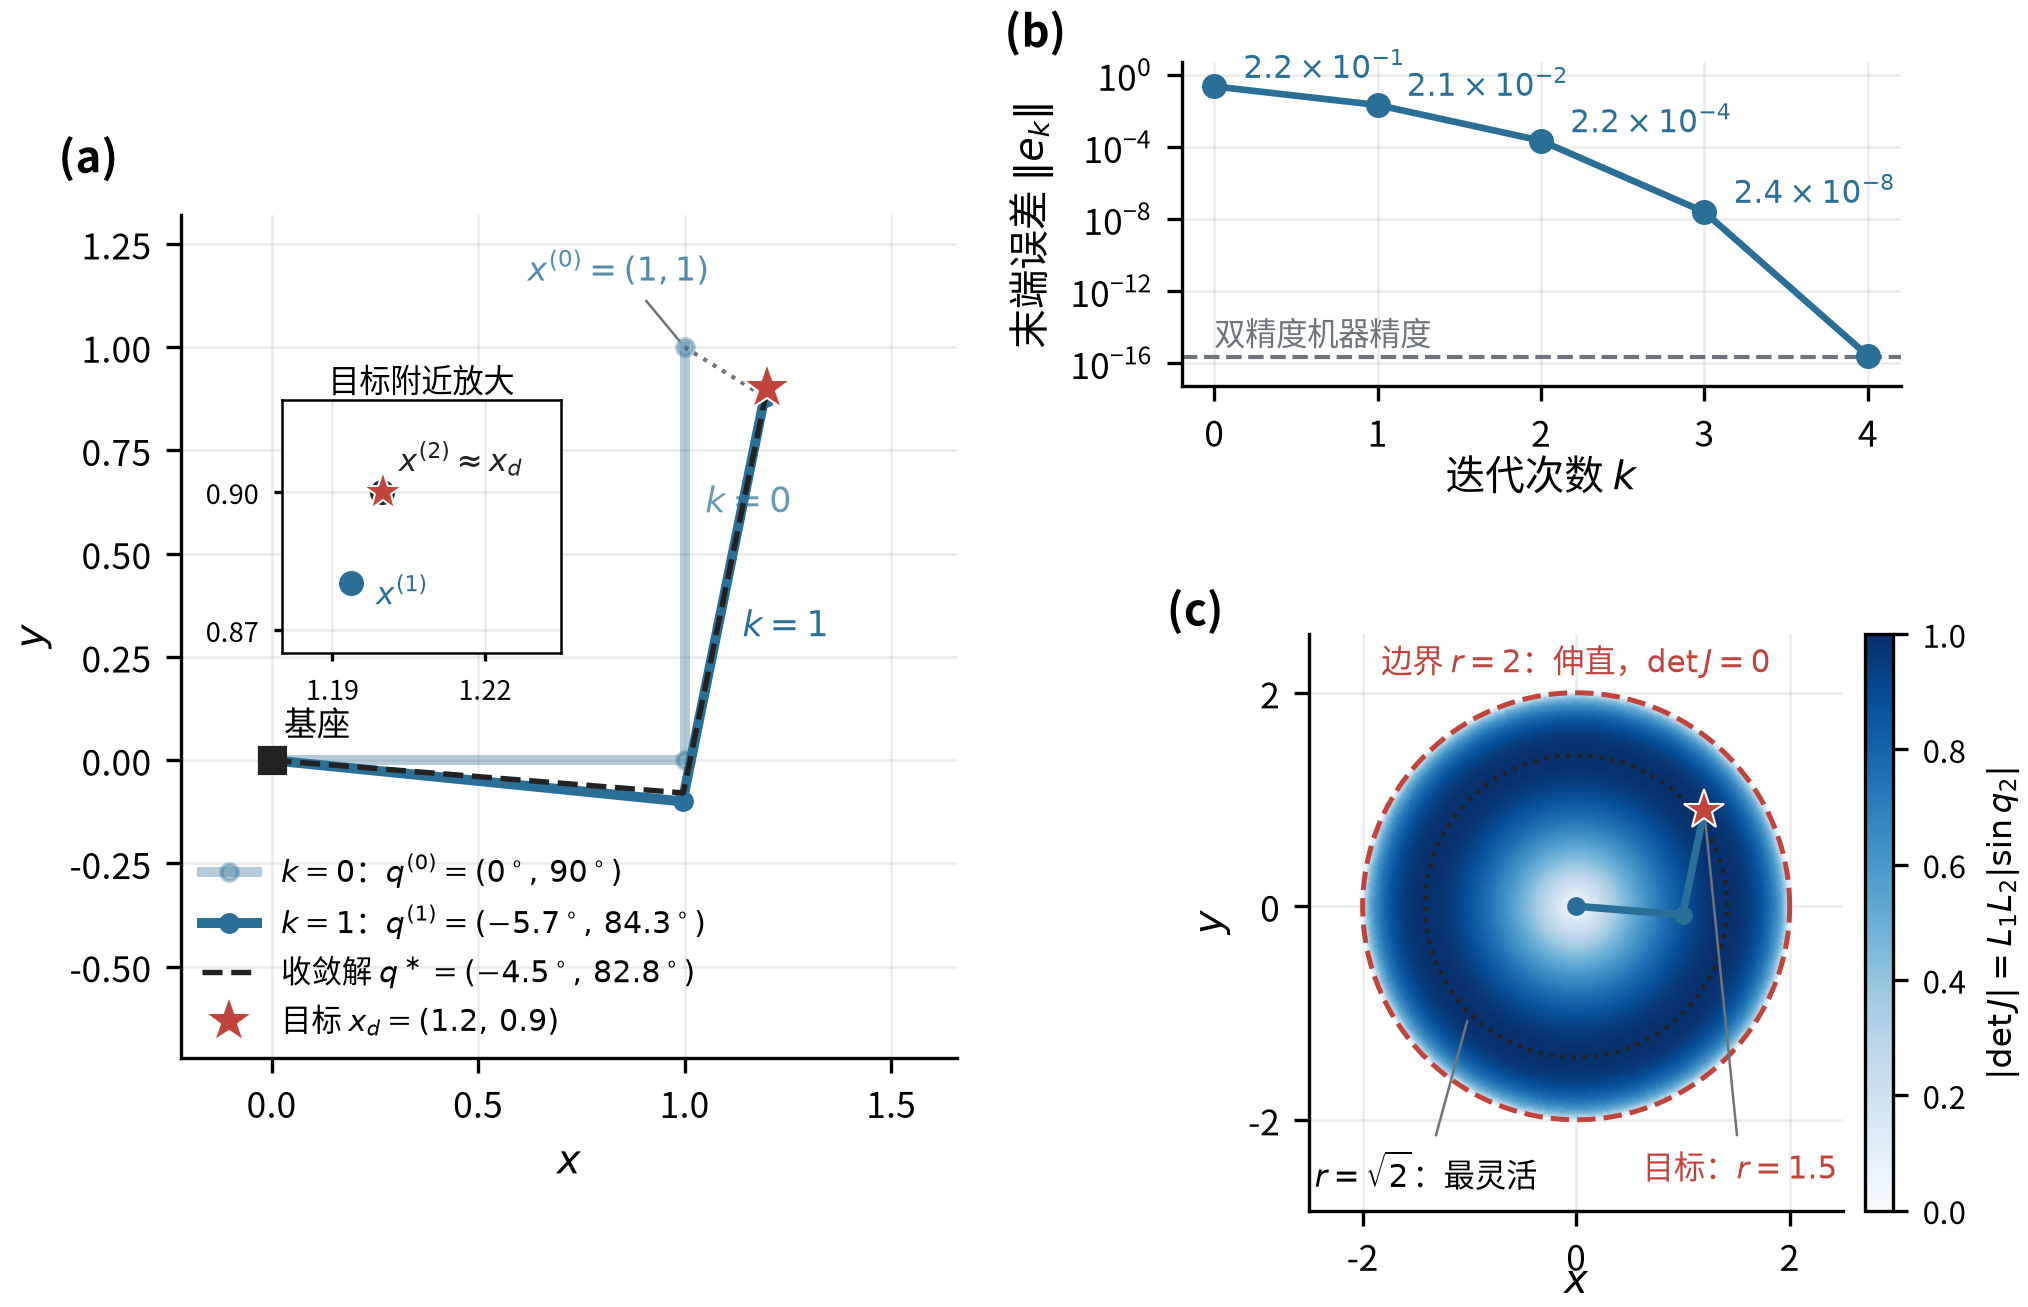
\includegraphics[width=0.98\textwidth]{figures/chap06/chap06_fig1.png}
\caption{牛顿迭代法求解逆运动学：与上面手算示例相同的设定（$L_1 = L_2 = 1$，目标 $x_d = (1.2,\,0.9)$，初值 $q^{(0)} = (0^\circ, 90^\circ)$），由 \texttt{code/chap07\_robotics.py} 实际迭代得到。（a）迭代过程中的机械臂姿态：一步之后末端到目标的距离已从 $0.22$ 缩到 $0.02$，两步之后与收敛解 $q^\ast = (-4.5^\circ,\,82.8^\circ)$ 肉眼已不可分（插图放大了目标附近）。（b）末端误差 $\|e_k\| = \|x_d - f(q^{(k)})\|$ 随迭代次数的变化（对数轴）：$2\times10^{-1} \to 2\times10^{-2} \to 2\times10^{-4} \to 2\times10^{-8}$，误差的指数每步大约翻一倍——这就是牛顿法的二次收敛，四步即达双精度机器精度。（c）工作空间上的可操作度 $|\det J| = L_1 L_2 |\sin q_2|$：外圈 $r = 2$（手臂伸直）与圆心是奇异位形，$r = \sqrt{2}$（$q_2 = 90^\circ$）处最灵活；目标点在 $r = 1.5$，离奇异位形很远，$J$ 良态，所以牛顿法收敛得又快又稳。}
\label{fig:chap06_robotics}
\end{figure}

\paragraph{当雅可比不可逆时怎么办？}

如果 $n > m$（冗余机械臂，$J$ 不是方阵），$J$ 没有逆。这时用\textbf{伪逆}（要求 $J$ 行满秩）：

\[
\Delta q = J^\dagger e, \quad \text{其中 } J^\dagger = J^\top(JJ^\top)^{-1}
\]

伪逆给出的是\textbf{最小范数解}——在所有能消除误差的 $\Delta q$ 中，选择最小的那个。在奇异位形附近 $JJ^\top$ 接近奇异，伪逆会“爆炸”，实践中改用阻尼最小二乘 $J^\top(JJ^\top + \delta^2 I)^{-1}$（习题 8）。
\clarify{伪逆不是“另一种方法”，它就是上一小节 KKT 条件的解：$\min \tfrac{1}{2}\|\Delta q\|^2$ s.t. $J\Delta q = e$ 给出 $\Delta q = -J^\top \lambda$，代回约束得 $\lambda = -(JJ^\top)^{-1} e$，于是 $\Delta q = J^\dagger e$。“最小范数解” = 拉格朗日乘子法的解。}

\begin{example}[几何解法 vs 迭代解法]
双连杆机械臂，$L_1 = L_2 = 1$，目标位置 $(1.0, 1.0)$。

\textbf{几何解法}（利用特殊结构）：

由于连杆等长，可以用余弦定理直接求解。

设末端到原点的距离为 $r = \sqrt{1^2 + 1^2} = \sqrt{2}$。

\begin{figure}[htbp]
\centering
\begin{tikzpicture}[scale=1.5]
    % 坐标系
    \draw[->] (-0.3,0) -- (1.8,0) node[right] {$x$};
    \draw[->] (0,-0.3) -- (0,1.8) node[above] {$y$};
    
    % 两种解
    % 解1：手肘朝上
    \draw[very thick, blue] (0,0) -- (0,1) -- (1,1);
    \fill[blue] (0,1) circle (2pt) node[left] {\small 肘};
    
    % 解2：手肘朝下（虚线）
    \draw[thick, blue, dashed] (0,0) -- (1,0) -- (1,1);
    \fill[blue, opacity=0.5] (1,0) circle (2pt) node[below] {\small 肘};
    
    % 目标点
    \fill[red] (1,1) circle (3pt) node[above right] {$(1,1)$};
    
    % 原点
    \fill (0,0) circle (2pt) node[below left] {$O$};
    
    % 距离标注
    \draw[<->, gray] (0.1,0.1) -- (0.9,0.9);
    \node[gray] at (0.7,0.3) {$r=\sqrt{2}$};
\end{tikzpicture}
\caption{逆运动学的两个解：手肘朝上或朝下}
\end{figure}

在三角形中，由余弦定理：
\[
r^2 = L_1^2 + L_2^2 - 2L_1 L_2 \cos(\pi - q_2)
\]

注意 $\pi - q_2$ 是三角形的内角，而 $q_2$ 是肘关节的弯曲角度。

代入数值：
\[
2 = 1 + 1 + 2 \cdot 1 \cdot 1 \cdot \cos q_2 \quad \Rightarrow \quad \cos q_2 = 0 \quad \Rightarrow \quad q_2 = \pm 90°
\]

于是有两个解：$q_2 = +90°$ 对应手肘朝上（图中实线），$q_2 = -90°$ 对应手肘朝下（图中虚线）。

取 $q_2 = 90°$，代入正运动学方程求 $q_1$：
\begin{align}
1 &= \cos q_1 + \cos(q_1 + 90°) = \cos q_1 - \sin q_1 \\
1 &= \sin q_1 + \sin(q_1 + 90°) = \sin q_1 + \cos q_1
\end{align}

两式相加：$2 = 2\cos q_1$，所以 $\cos q_1 = 1$，$q_1 = 0°$。

\textbf{验证}：
\[
x = \cos 0° + \cos 90° = 1 + 0 = 1 \quad \checkmark
\]
\[
y = \sin 0° + \sin 90° = 0 + 1 = 1 \quad \checkmark
\]

\textbf{总结}：几何解法快速直接，但只适用于简单结构。牛顿迭代法适用于任意复杂的机械臂。
\end{example}

\subsection{冗余机械臂与零空间}

\paragraph{什么是冗余？}

当机械臂的关节数 $n$ 大于任务空间维度 $m$ 时，我们说它是\textbf{冗余}的。

\begin{center}
\renewcommand{\arraystretch}{1.3}
\begin{tabular}{l|c|c|l}
\toprule
\textbf{例子} & \textbf{关节数 $n$} & \textbf{任务维度 $m$} & \textbf{冗余度 $n-m$} \\
\midrule
平面双连杆 & 2 & 2 & 0（恰好） \\
典型工业臂 & 6 & 6 & 0（恰好） \\
人的手臂 & 7 & 6 & 1 \\
双臂机器人 & 14 & 6（单手任务） & 8 \\
蛇形机器人 & 20+ & 6 & 14+ \\
\bottomrule
\end{tabular}
\end{center}

\paragraph{冗余意味着什么？}

冗余意味着逆运动学有\textbf{无穷多解}。直觉上：完成同一个任务，有很多种姿势可以选择。

\begin{example}[人手臂的冗余]
做一个实验：把你的手掌放在桌面上固定不动，然后在保持手掌位置和朝向不变的前提下移动你的手肘。你会发现，手肘可以在一个弧线上移动，而手掌完全不动——这就是冗余带来的自由度。正是这个“额外”的自由度，让我们能在狭窄空间里绕开障碍物、避免撞到自己的身体，或者干脆换一个更舒服的姿势。
\end{example}

\paragraph{零空间的数学描述}\mbox{}\par\nopagebreak

\begin{definition}[零空间]
雅可比矩阵 $J$ 的\textbf{零空间}（Null Space）是所有满足 $J v = 0$ 的向量 $v$ 的集合：
\[
\mathcal{N}(J) = \{ v \in \mathbb{R}^n : Jv = 0 \}
\]
\end{definition}

\textbf{物理意义}：如果关节速度 $\dot{q}$ 在零空间中，那么 $\dot{x} = J\dot{q} = 0$——末端不动！

换句话说，零空间运动是“内部运动”——关节在动，但末端静止。

\begin{figure}[htbp]
\centering
\begin{tikzpicture}[scale=1.0]
    % 左图：三连杆机械臂，两种构型
    \begin{scope}[shift={(0,0)}]
        \node at (2,-2) {\textbf{(a) 三连杆机械臂}};
        
        % 构型1
        \draw[very thick, blue] (0,0) -- (1,1.5) -- (2.5,1.8) -- (3.5,1);
        \fill (0,0) circle (2pt);
        \fill (1,1.5) circle (2pt);
        \fill (2.5,1.8) circle (2pt);
        \fill[red] (3.5,1) circle (3pt);
        
        % 构型2（虚线）
        \draw[thick, blue, dashed] (0,0) -- (1.5,0.8) -- (2.8,1.5) -- (3.5,1);
        \fill[blue, opacity=0.3] (1.5,0.8) circle (2pt);
        \fill[blue, opacity=0.3] (2.8,1.5) circle (2pt);
        
        % 说明
        \node[red] at (3.5,0.5) {\small 末端固定};
        \draw[<->, dashed, gray] (1,1.5) .. controls (1.3,1.1) .. (1.5,0.8);
        \node[gray] at (0.5,1) {\scriptsize 零空间运动};
    \end{scope}
    
    % 右图：零空间示意
    \begin{scope}[shift={(7,0)}]
        \node at (2,-2) {\textbf{(b) 零空间示意}};
        
        % 关节空间
        \draw[->] (0,0) -- (3.5,0) node[right] {$\dot{q}_1$};
        \draw[->] (0,0) -- (0,2.5) node[above] {$\dot{q}_2$};
        
        % 零空间（一条线）
        \draw[very thick, green!60!black] (-0.5,-0.3) -- (3,1.8);
        \node[green!60!black] at (3.2,2) {$\mathcal{N}(J)$};
        
        % 一个向量
        \draw[->, thick, blue] (0,0) -- (2,1.2);
        \node[blue] at (1.5,0.5) {$\dot{q} \in \mathcal{N}(J)$};
        
        % 说明
        \node at (1.5,-0.8) {\small 沿此方向运动};
        \node at (1.5,-1.2) {\small 末端速度为零};
    \end{scope}
\end{tikzpicture}
\caption{零空间运动：关节在动，末端不动}
\end{figure}

\paragraph{冗余逆运动学的通解}

当 $n > m$ 时，逆运动学的解可以写成：

\begin{keyformula}[title=冗余逆运动学的通解]
\begin{equation}
\dot{q} = \underbrace{J^\dagger \dot{x}_d}_{\text{完成主任务}} + \underbrace{(I - J^\dagger J) z}_{\text{零空间运动}}
\end{equation}
其中 $J^\dagger = J^\top(JJ^\top)^{-1}$ 是\textbf{伪逆}，$\dot{x}_d$ 是期望的末端速度，$(I - J^\dagger J)$ 是\textbf{零空间投影矩阵}，而 $z \in \mathbb{R}^n$ 是\textbf{任意向量}。
\end{keyformula}

\begin{physicalmeaning}
这个公式把关节速度拆成了两部分。第一项 $J^\dagger \dot{x}_d$ 保证末端以期望速度 $\dot{x}_d$ 运动；第二项 $(I - J^\dagger J) z$ 落在零空间中，所以无论 $z$ 取什么，它都不影响末端。于是 $z$ 可以自由选择，用来实现\textbf{次级目标}。
\end{physicalmeaning}

\paragraph{次级目标的例子}

$z$ 可以怎么选？常见的做法是取某个标量函数的梯度，让零空间运动顺着它上升或下降。若想\textbf{远离关节限位}，可取
\[
z = -k \nabla_q W(q), \quad W(q) = \sum_i \frac{1}{(q_i - q_i^{min})(q_i^{max} - q_i)}
\]
$W$ 在关节接近限位时变大，负梯度方向指向“远离限位”。若想\textbf{避开障碍物}，可取 $z = k \nabla_q d(q)$，其中 $d(q)$ 是机械臂与障碍物的最近距离，沿梯度方向走就是把距离拉大。若想\textbf{最小化能量}，则取 $z = -k \nabla_q \|\tau\|^2$，让关节力矩尽可能小。

\begin{example}[冗余的实际应用]
想象一个7自由度机械臂在一个有障碍物的环境中工作：

\begin{figure}[htbp]
\centering
\begin{tikzpicture}[scale=0.9]
    % 障碍物
    \fill[gray!40] (2,0.5) rectangle (2.5,2);
    \node at (2.25,2.3) {\small 障碍物};
    
    % 构型1：会撞到障碍物
    \draw[thick, red, dashed] (0,0) -- (1,1) -- (2.2,1.2) -- (3.5,0.8);
    \fill[red, opacity=0.5] (2.2,1.2) circle (3pt);
    \node[red] at (1.5,1.5) {\small 碰撞！};
    
    % 构型2：绕开障碍物
    \draw[very thick, blue] (0,0) -- (0.8,1.5) -- (1.5,2.2) -- (3.5,0.8);
    \fill (0,0) circle (2pt);
    \fill (0.8,1.5) circle (2pt);
    \fill (1.5,2.2) circle (2pt) node[above] {\small 肘抬高};
    \fill[red] (3.5,0.8) circle (3pt) node[right] {\small 末端};
    
    % 说明
    \node at (1.75,-0.5) {\small 利用零空间绕开障碍物};
\end{tikzpicture}
\caption{冗余自由度让机械臂能够在保持末端位置的同时避开障碍物}
\end{figure}

两种构型的末端位置相同，但只有蓝色构型能避开障碍物。冗余自由度提供了这种灵活性。
\end{example}
\preview{第7章会把“选一个 $z$ 做次级目标”升级为对整条轨迹 $q(t)$ 做优化：动力学约束用拉格朗日乘子（伴随变量）处理，这就是轨迹优化和 MPC。}

% ------------------------------------------------------------------------------------
\section{机器人动力学：力与运动的关系}

\subsection{为什么需要动力学？}

到目前为止，我们讨论的运动学只关心\textbf{几何关系}——关节角度和末端位置的对应。但实际控制机器人时，我们需要知道：

\begin{quote}
\textit{电机应该输出多大的力矩，才能让机械臂按照期望的方式运动？}
\end{quote}

这就是\textbf{动力学}要回答的问题。

\begin{example}[直觉理解]
想象你在举哑铃。哑铃越重，举起它需要的力越大，这是质量的作用；想举得越快，需要的力也越大，这是加速度的作用；即使哑铃静止不动，你也得持续用力来抵抗重力；而如果哑铃在转动，你还会感到一些“奇怪”的力——科氏力和离心力。机器人动力学就是要把这些直觉变成精确的数学公式。
\end{example}

\subsection{复习：拉格朗日方程}

在第5章，我们学过拉格朗日方程：
\begin{equation}
\frac{d}{dt}\frac{\partial L}{\partial \dot{q}_i} - \frac{\partial L}{\partial q_i} = Q_i
\end{equation}

其中 $L = T - V$ 是拉格朗日量（动能减势能），$q_i$ 是广义坐标，对机器人来说就是关节角度，$Q_i$ 是广义力，对机器人来说就是关节力矩 $\tau_i$。

这个方程的美妙之处在于：只要写出动能和势能的表达式，力学方程就自动出来了！
\clarify{第5章的拉格朗日方程右边是 0，广义力 $F_i = \partial L/\partial q_i$ 指的是保守力（势能的负梯度）。这里右边的 $Q_i$ 是电机、摩擦这类不能写进势能的外力——它们必须单独加在右边。}

\subsection{机器人的动能}

\paragraph{单连杆的动能}

考虑一根绕端点转动的杆（单摆），质量 $m$，长度 $L$，假设质量集中在末端：

\begin{figure}[htbp]
\centering
\begin{tikzpicture}[scale=1.2]
    % 固定点
    \fill (0,0) circle (2pt);
    \draw[thick] (-0.3,0.1) -- (0.3,0.1);
    \draw[thick] (-0.25,0.1) -- (-0.25,0.2);
    \draw[thick] (0,0.1) -- (0,0.2);
    \draw[thick] (0.25,0.1) -- (0.25,0.2);
    
    % 连杆
    \draw[very thick, blue] (0,0) -- ({1.5*sin(40)},{-1.5*cos(40)});
    
    % 质点
    \fill[red] ({1.5*sin(40)},{-1.5*cos(40)}) circle (4pt);
    \node[red, right] at ({1.5*sin(40)+0.1},{-1.5*cos(40)}) {$m$};
    
    % 角度
    \draw[dashed] (0,0) -- (0,-1.5);
    \draw[->] (0,-0.8) arc (-90:-50:0.8);
    \node at (0.4,-0.6) {$q$};
    
    % 长度
    \draw[<->] (0.15,0) -- ({1.5*sin(40)+0.15},{-1.5*cos(40)});
    \node[right] at ({0.75*sin(40)+0.2},{-0.75*cos(40)}) {$L$};
    
    % 速度
    \draw[->, thick, green!60!black] ({1.5*sin(40)},{-1.5*cos(40)}) -- 
        ({1.5*sin(40)+0.8*cos(40)},{-1.5*cos(40)+0.8*sin(40)});
    \node[green!60!black] at ({1.5*sin(40)+1},{-1.5*cos(40)+0.3}) {$v = L\dot{q}$};
\end{tikzpicture}
\caption{单摆：最简单的“机器人”}
\end{figure}

质点的速度大小为 $v = L\dot{q}$（圆周运动），所以动能是：
\begin{equation}
T = \frac{1}{2}mv^2 = \frac{1}{2}m(L\dot{q})^2 = \frac{1}{2}mL^2 \dot{q}^2
\end{equation}

我们可以定义\textbf{转动惯量} $I = mL^2$，则 $T = \frac{1}{2}I\dot{q}^2$。

\paragraph{多连杆的动能}

对于多连杆机械臂，每个连杆都在运动，总动能是各部分之和。关键观察是：每个连杆的速度取决于\textbf{所有它之前的关节}的角度和角速度。

最终，总动能可以写成：
\begin{equation}
T = \frac{1}{2} \dot{q}^\top M(q) \dot{q}
\end{equation}

其中 $M(q)$ 是 $n \times n$ 的\textbf{质量矩阵}（也叫惯性矩阵）。

\begin{physicalmeaning}
$M(q)$ 的每个元素都有物理意义：对角元 $M_{ii}$ 是第 $i$ 个关节单独转动时的“有效惯量”，非对角元 $M_{ij}$（$i \neq j$）是关节 $i$ 和 $j$ 之间的“惯性耦合”。整个矩阵依赖于位形 $q$——机械臂伸直时和弯曲时，惯量不同！
\end{physicalmeaning}

\begin{example}[伸直 vs 弯曲的惯量]
想象一根双连杆机械臂：

\begin{figure}[htbp]
\centering
\begin{tikzpicture}[scale=1.0]
    % 伸直
    \begin{scope}[shift={(0,0)}]
        \draw[very thick, blue] (0,0) -- (2,0) -- (4,0);
        \fill (0,0) circle (2pt);
        \fill (2,0) circle (2pt);
        \fill[red] (4,0) circle (3pt);
        \draw[->] (0,-0.5) arc (-90:0:0.5);
        \node at (0.7,-0.3) {$\dot{q}_1$};
        \node at (2,-1) {\small 伸直：转动惯量大};
    \end{scope}
    
    % 弯曲
    \begin{scope}[shift={(6,0)}]
        \draw[very thick, blue] (0,0) -- (1.5,0) -- (1.5,-1.5);
        \fill (0,0) circle (2pt);
        \fill (1.5,0) circle (2pt);
        \fill[red] (1.5,-1.5) circle (3pt);
        \draw[->] (0,-0.5) arc (-90:0:0.5);
        \node at (0.7,-0.3) {$\dot{q}_1$};
        \node at (1,-2) {\small 弯曲：转动惯量小};
    \end{scope}
\end{tikzpicture}
\caption{质量矩阵依赖于位形}
\end{figure}

当手臂伸直时，末端离肩关节很远，绕肩关节转动时需要更大的力矩。这体现在 $M_{11}$ 更大。

当手臂弯曲时，末端离肩关节近，转动惯量变小。
\end{example}

\subsection{机器人的势能}

对于大多数机器人，势能只来自重力：
\begin{equation}
V = \sum_i m_i g h_i(q)
\end{equation}

其中 $h_i(q)$ 是第 $i$ 个连杆质心的高度（取决于关节角度 $q$）。

\subsection{推导动力学方程}

现在让我们用拉格朗日方程推导机器人的动力学。

\paragraph{第一步：计算 $\frac{\partial L}{\partial \dot{q}}$}

\begin{align}
\frac{\partial L}{\partial \dot{q}} &= \frac{\partial T}{\partial \dot{q}} - \frac{\partial V}{\partial \dot{q}} \\
&= \frac{\partial}{\partial \dot{q}} \left( \frac{1}{2} \dot{q}^\top M(q) \dot{q} \right) - 0 \\
&= M(q) \dot{q}
\end{align}

（这里用到了 $\frac{\partial}{\partial x}(x^\top A x) = 2Ax$ 对于对称矩阵 $A$。）

\paragraph{第二步：计算 $\frac{d}{dt}\frac{\partial L}{\partial \dot{q}}$}

\begin{align}
\frac{d}{dt}(M(q)\dot{q}) &= \dot{M}(q)\dot{q} + M(q)\ddot{q}
\end{align}

这里 $\dot{M}$ 是 $M$ 对时间的导数，它依赖于 $\dot{q}$。

\paragraph{第三步：计算 $\frac{\partial L}{\partial q}$}

\begin{align}
\frac{\partial L}{\partial q} &= \frac{\partial T}{\partial q} - \frac{\partial V}{\partial q}
\end{align}

$\frac{\partial T}{\partial q}$ 来自 $M(q)$ 对 $q$ 的依赖，$\frac{\partial V}{\partial q}$ 是重力产生的力。

\paragraph{第四步：整理}

把所有项放在一起，经过仔细整理（具体推导需要一些技巧），最终得到：

\begin{keyformula}[title=机器人动力学标准形式]
\begin{equation}
\boxed{M(q)\ddot{q} + C(q, \dot{q})\dot{q} + G(q) = \tau}
\end{equation}
\end{keyformula}

\begin{center}
\renewcommand{\arraystretch}{1.5}
\begin{tabular}{c|l|p{7cm}}
\toprule
\textbf{符号} & \textbf{名称} & \textbf{物理意义} \\
\midrule
$M(q)\ddot{q}$ & 惯性项 & 加速关节需要的力矩，就像 $F = ma$ \\
$C(q, \dot{q})\dot{q}$ & 科氏力/离心力 & 速度引起的“假想力”，旋转坐标系中才有 \\
$G(q)$ & 重力项 & 抵抗重力需要的力矩 \\
$\tau$ & 关节力矩 & 电机需要输出的力矩 \\
\bottomrule
\end{tabular}
\end{center}

\begin{example}[单摆的完整推导]
让我们对单摆完整做一遍拉格朗日推导。

\textbf{设置}：质量 $m$，长度 $L$，关节角 $q$（从竖直向下测量）。

\textbf{动能}：
\[
T = \frac{1}{2}mL^2\dot{q}^2
\]

\textbf{势能}（以铰链为零势能点）：
\[
V = -mgL\cos q
\]

注意：当 $q = 0$（竖直向下）时，$V = -mgL$（最低）；当 $q = 90°$（水平）时，$V = 0$。

\textbf{拉格朗日量}：
\[
L = T - V = \frac{1}{2}mL^2\dot{q}^2 + mgL\cos q
\]

\textbf{计算各项}：
\begin{align}
\frac{\partial L}{\partial \dot{q}} &= mL^2\dot{q} \\
\frac{d}{dt}\frac{\partial L}{\partial \dot{q}} &= mL^2\ddot{q} \\
\frac{\partial L}{\partial q} &= -mgL\sin q
\end{align}

\textbf{拉格朗日方程}：
\[
mL^2\ddot{q} - (-mgL\sin q) = \tau
\]

即：
\[
\boxed{mL^2\ddot{q} + mgL\sin q = \tau}
\]

\textbf{对比标准形式}：$M = mL^2$ 是常数，因为单摆只有一个关节；$C = 0$，单关节没有科氏力；$G = mgL\sin q$ 是重力产生的力矩。

\textbf{物理检验}：当 $q = 0$（竖直向下）时 $G = 0$，不需要力矩来维持；当 $q = 90°$（水平）时 $G = mgL$，需要的力矩最大；当 $q = 180°$（竖直向上）时 $G$ 又回到 0，但这是不稳定平衡。
\end{example}

\begin{example}[双连杆机械臂的动力学（概念性）]
对于双连杆机械臂，动力学方程会更复杂。质量矩阵是 $2 \times 2$：

\[
M(q) = \begin{bmatrix}
M_{11}(q_2) & M_{12}(q_2) \\
M_{12}(q_2) & M_{22}
\end{bmatrix}
\]

这里 $M_{11}$ 依赖于肘关节角度 $q_2$：手臂弯曲时，肩关节的有效惯量变小；$M_{22}$ 是常数，肘关节的惯量不受其他关节影响；而 $M_{12} = M_{21}$，这个对称性来自动能的二次型性质。

科氏力矩阵 $C$ 包含 $\dot{q}_1^2$ 和 $\dot{q}_1\dot{q}_2$ 等项——这些是快速运动时产生的“假想力”。

重力向量 $G$ 包含 $\sin$ 和 $\cos$ 项——取决于各连杆的角度。

具体表达式很长，通常用符号计算软件导出。
\end{example}

\subsection{动力学的重要性质}

机器人动力学有几个重要的数学性质，它们对控制设计很有用：

\paragraph{性质1：质量矩阵对称正定}
\[
M(q) = M(q)^\top, \quad M(q) > 0
\]

\textbf{物理意义}：动能 $T = \frac{1}{2}\dot{q}^\top M \dot{q}$ 总是正的（只要有运动）。

\paragraph{性质2：$\dot{M} - 2C$ 反对称}
\[
\dot{q}^\top (\dot{M} - 2C) \dot{q} = 0
\]

\textbf{物理意义}：这保证了能量守恒。如果没有外力（$\tau = 0$）且忽略重力，系统能量 $T$ 保持不变。

\begin{proof}[简单说明]
对动能求时间导数：
\begin{align}
\frac{dT}{dt} &= \frac{d}{dt}\left(\frac{1}{2}\dot{q}^\top M \dot{q}\right) \\
&= \frac{1}{2}\dot{q}^\top \dot{M} \dot{q} + \dot{q}^\top M \ddot{q}
\end{align}

把 $M\ddot{q} = \tau - C\dot{q} - G$ 代入：
\begin{align}
\frac{dT}{dt} &= \frac{1}{2}\dot{q}^\top \dot{M} \dot{q} + \dot{q}^\top (\tau - C\dot{q} - G) \\
&= \dot{q}^\top \tau - \dot{q}^\top G + \frac{1}{2}\dot{q}^\top (\dot{M} - 2C) \dot{q}
\end{align}

如果 $\dot{M} - 2C$ 反对称，最后一项为零，于是：
\[
\frac{dT}{dt} = \dot{q}^\top \tau - \dot{q}^\top G = \text{功率输入} - \text{重力功率}
\]

这正是能量守恒的表达！
\end{proof}

\paragraph{性质3：线性于参数}

动力学方程可以写成：
\[
M(q)\ddot{q} + C(q,\dot{q})\dot{q} + G(q) = Y(q, \dot{q}, \ddot{q}) \theta
\]

其中 $Y$ 是已知的矩阵（只依赖于运动状态），$\theta$ 是物理参数向量（质量、惯量、质心位置等）。

\textbf{应用}：这个性质让我们能够通过测量运动和力矩来\textbf{辨识}机器人的物理参数。

% ------------------------------------------------------------------------------------
\section{接触力学：当机器人碰到东西时}

\subsection{为什么接触很重要？}

机器人与世界交互几乎总是通过接触：机械臂抓取物体、腿式机器人行走、工业机器人装配零件、手术机器人操作组织，无一例外。没有接触力的分析，我们无法理解机器人如何真正“做事”。

\begin{example}[行走的秘密]
当你走路时，脚蹬地，地面给你一个向前的摩擦力，推动你前进。

如果地面是完美光滑的（没有摩擦），你只能原地踏步——就像在冰面上一样。

机器人行走也是如此：地面反作用力是推动机器人前进的“动力来源”。
\end{example}

\subsection{接触力如何进入动力学方程}

当机器人与环境接触时，接触点受到\textbf{接触力} $\lambda_c$。这个力如何影响关节运动？

答案是通过\textbf{雅可比转置}——和末端力传递完全一样！

\begin{keyformula}[title=带接触的动力学方程]
\begin{equation}
M(q)\ddot{q} + C(q,\dot{q})\dot{q} + G(q) = \tau + J_c(q)^\top \lambda_c
\end{equation}

其中 $J_c(q)$ 是接触点的雅可比矩阵，$\lambda_c$ 是作用在接触点处的接触力，$J_c^\top \lambda_c$ 则是接触力在关节空间产生的\textbf{广义力}。
\end{keyformula}

\begin{keyformula}[title=接触动力学的 KKT 形式]
保持接触时 $\phi(q) \equiv 0$，对时间求两次导得 $J_c \ddot{q} + \dot{J}_c \dot{q} = 0$。把它和动力学方程并起来：
\begin{equation}
\begin{bmatrix} M(q) & -J_c^\top \\ J_c & 0 \end{bmatrix}
\begin{bmatrix} \ddot{q} \\ \lambda_c \end{bmatrix}
=
\begin{bmatrix} \tau - C\dot{q} - G \\ -\dot{J}_c \dot{q} \end{bmatrix}
\end{equation}
对比第1章的 KKT 矩阵 $\begin{bmatrix} \nabla^2_{xx}\Lag & (\nabla g)^\top \\ \nabla g & 0 \end{bmatrix}$（符号约定不同，结构相同）：质量矩阵 $M$ 扮演 Hessian，约束雅可比 $J_c$ 扮演 $\nabla g$，接触力 $\lambda_c$ 就是乘子。这正是“高斯最小拘束原理”：在所有满足接触约束的加速度中，真实的 $\ddot{q}$ 使 $\tfrac{1}{2}(\ddot{q} - \ddot{q}_{\text{free}})^\top M (\ddot{q} - \ddot{q}_{\text{free}})$ 最小（$\ddot{q}_{\text{free}} = M^{-1}(\tau - C\dot{q} - G)$ 是无接触时的加速度），$\lambda_c$ 是这个二次规划的乘子。
\end{keyformula}
\review{第1章}{第1章扩展阅读预告过：KKT 矩阵会在本章以“质量矩阵 + 约束雅可比”的形式出现——就是上面这个分块矩阵。第1章思考题 9 的答案也在这里：$H \leftrightarrow M$，$\nabla g \leftrightarrow J_c$，$\lambda \leftrightarrow$ 接触力。}

\begin{physicalmeaning}
$J_c^\top$ 把接触点的力“传递”到关节空间，就像 $J^\top$ 把末端力传递到关节一样。

这正是我们在约束优化中见过的\textbf{拉格朗日乘子}！$\lambda_c$ 是接触约束的乘子，它自动给出了维持约束所需的力。
\end{physicalmeaning}

\subsection{接触力的物理约束}

接触力不是任意的，它必须满足物理约束：

\paragraph{约束1：不能穿透}

设 $\phi(q)$ 是接触间隙，即机器人与环境之间的最近距离：$\phi > 0$ 表示没有接触，$\phi = 0$ 表示正在接触，而 $\phi < 0$ 意味着穿透，物理上不允许。于是约束是 $\phi(q) \geq 0$。

\paragraph{约束2：法向力是推力}

接触面只能“推”不能“拉”（除非有吸盘）：
\[
\lambda_n \geq 0
\]

其中 $\lambda_n$ 是法向接触力。

\paragraph{约束3：互补松弛}

这是最关键的条件：
\[
\lambda_n \cdot \phi(q) = 0
\]

它的含义是两者至少有一个为零：如果 $\phi > 0$（不接触），则 $\lambda_n = 0$（没有力）；反过来，如果 $\lambda_n > 0$（有力），则必有 $\phi = 0$（正在接触）。

\begin{figure}[htbp]
\centering
\begin{tikzpicture}[scale=1.4]
    % 地面
    \fill[gray!20] (-0.5,-0.1) rectangle (8,0);
    \draw[thick] (-0.5,0) -- (8,0);
    
    % 状态1：悬空
    \begin{scope}[shift={(1,0)}]
        \draw[thick, blue, fill=blue!20] (0,1) circle (0.4);
        \node at (0,1) {\small 球};
        \draw[->, red, thick] (0,0.6) -- (0,0.15) node[right] {$mg$};
        
        \node at (0,-0.4) {\small $\phi > 0$};
        \node at (0,-0.7) {\small $\lambda = 0$};
        \node at (0,1.7) {\small \textbf{悬空}};
    \end{scope}
    
    % 状态2：静止接触
    \begin{scope}[shift={(3.5,0)}]
        \draw[thick, blue, fill=blue!20] (0,0.4) circle (0.4);
        \node at (0,0.4) {\small 球};
        \draw[->, red, thick] (0,0.4) -- (0,-0.25) node[right] {$mg$};
        \draw[->, green!60!black, thick] (0,0) -- (0,0.65) node[left] {$\lambda$};
        
        \node at (0,-0.4) {\small $\phi = 0$};
        \node at (0,-0.7) {\small $\lambda = mg$};
        \node at (0,1.1) {\small \textbf{静止接触}};
    \end{scope}
    
    % 状态3：滑动接触
    \begin{scope}[shift={(6,0)}]
        \draw[thick, blue, fill=blue!20] (0,0.4) circle (0.4);
        \node at (0,0.4) {\small 球};
        \draw[->, red, thick] (0,0.4) -- (0,-0.25);
        \draw[->, green!60!black, thick] (0,0) -- (0,0.65);
        \draw[->, orange, thick] (0,0) -- (0.5,0) node[above] {$f$};
        \draw[->, blue, thick] (0.4,0.4) -- (0.9,0.4) node[above] {$v$};
        
        \node at (0,-0.4) {\small $\phi = 0$};
        \node at (0,-0.7) {\small $|f| = \mu\lambda$};
        \node at (0,1.1) {\small \textbf{滑动接触}};
    \end{scope}
\end{tikzpicture}
\caption{接触的三种状态}
\end{figure}

\begin{insightbox}
互补松弛条件 $\lambda \cdot \phi = 0$ 和第2章线性规划中的互补松弛完全一样！

在线性规划中：“免费的资源没人用，稀缺的资源才有价格”。

在接触力学中：“悬空时没有力，接触时才有力”。

这是同一个数学结构在不同领域的体现。
\end{insightbox}
\review{第2章}{第2章的互补松弛：对偶变量 $y_i$ 和松弛量 $s_i$ 至少一个为零——“免费的资源没人用，稀缺的资源才有价格”。把 $y_i$ 换成 $\lambda_n$、$s_i$ 换成间隙 $\phi$，就是这里的条件。}

\subsection{摩擦力与库仑锥}

除了法向力，接触通常还有\textbf{摩擦力}（切向力）。

\paragraph{库仑摩擦模型}

最常用的摩擦模型是库仑模型。它区分两种情形：物体静止时是静摩擦，摩擦力可以指向任意方向，但大小受限；物体滑动时是动摩擦，摩擦力与速度方向相反，大小正比于法向力。两种情形合起来写成一个不等式：
\[
\|f_t\| \leq \mu \lambda_n
\]

其中 $f_t$ 是切向力，$\mu$ 是摩擦系数，$\lambda_n$ 是法向力。

\paragraph{摩擦锥}

这个不等式定义了一个\textbf{锥形区域}：接触力必须在锥内。

\begin{figure}[htbp]
\centering
\begin{tikzpicture}[scale=1.2]
    % 三维摩擦锥
    \begin{scope}[shift={(0,0)}]
        % 底面（椭圆表示圆）
        \draw[thick, gray, dashed] (0,0) ellipse (1.5 and 0.5);
        
        % 锥面
        \draw[thick, green!60!black, fill=green!10, opacity=0.5] 
            (0,0) -- (-1.5,0) -- (0,2.5) -- cycle;
        \draw[thick, green!60!black, fill=green!10, opacity=0.5] 
            (0,0) -- (1.5,0) -- (0,2.5) -- cycle;
        \draw[thick, green!60!black] (0,0) -- (0,2.5);
        
        % 顶点
        \fill (0,0) circle (2pt);
        
        % 一个可行的力
        \draw[->, very thick, blue] (0,0) -- (0.5,1.8);
        \node[blue, right] at (0.5,1.8) {$\lambda$（可行）};
        
        % 一个不可行的力
        \draw[->, very thick, red, dashed] (0,0) -- (1.8,0.8);
        \node[red, right] at (1.8,0.8) {（滑动）};
        
        % 标注
        \node at (0,-1.2) {\small 法向：$\lambda_n$};
        \draw[<->] (-1.7,0) -- (-1.7,2.5) node[midway, left] {\small $\lambda_n$};
        \draw[<->] (-1.5,-0.7) -- (1.5,-0.7) node[midway, below] {\small $\mu\lambda_n$};
    \end{scope}
    
    % 二维示意
    \begin{scope}[shift={(5,0)}]
        % 地面
        \fill[gray!20] (-1.5,-0.1) rectangle (1.5,0);
        \draw[thick] (-1.5,0) -- (1.5,0);
        
        % 摩擦锥（二维）
        \fill[green!20, opacity=0.5] (0,0) -- (-1,2) -- (1,2) -- cycle;
        \draw[thick, green!60!black] (0,0) -- (-1,2);
        \draw[thick, green!60!black] (0,0) -- (1,2);
        
        % 角度标注
        \draw[dashed] (0,0) -- (0,2);
        \draw (0,0.8) arc (90:117:0.8);
        \node at (-0.4,1) {\small $\theta$};
        \node at (1.3,1.5) {\small $\tan\theta = \mu$};
        
        % 说明
        \node at (0,-0.8) {\small 二维摩擦锥};
    \end{scope}
\end{tikzpicture}
\caption{摩擦锥：接触力必须在锥内才能保持静止}
\end{figure}

\paragraph{摩擦锥与优化}

摩擦锥约束 $\|f_t\| \leq \mu \lambda_n$ 是一个\textbf{二阶锥约束}（Second-Order Cone Constraint）。

带摩擦的接触问题可以写成\textbf{二阶锥规划}（SOCP），这是凸优化的一种，可以高效求解。

\begin{example}[机器人抓取]
当机械臂抓取一个物体时，手指与物体之间的接触力必须同时满足三件事：法向力为正（推而不拉），摩擦力在锥内（不滑动），并且各接触力的合力平衡物体重力。这是一个带锥约束的力平衡问题，可以用凸优化求解最优抓取力。

\begin{figure}[htbp]
\centering
\begin{tikzpicture}[scale=1.0]
    % 物体
    \fill[blue!20] (0,0) rectangle (2,1.5);
    \draw[thick] (0,0) rectangle (2,1.5);
    \node at (1,0.75) {物体};
    
    % 左手指
    \fill[gray!40] (-0.5,0.4) rectangle (0,1.1);
    \draw[thick] (-0.5,0.4) rectangle (0,1.1);
    
    % 右手指
    \fill[gray!40] (2,0.4) rectangle (2.5,1.1);
    \draw[thick] (2,0.4) rectangle (2.5,1.1);
    
    % 接触力
    \draw[->, thick, green!60!black] (0,0.75) -- (0.7,0.75) node[above] {$\lambda_1$};
    \draw[->, thick, green!60!black] (2,0.75) -- (1.3,0.75) node[above] {$\lambda_2$};
    
    % 重力
    \draw[->, thick, red] (1,0) -- (1,-0.7) node[right] {$mg$};
    
    % 摩擦锥示意
    \draw[dashed, green!60!black] (0,0.75) -- (0.4,1.1);
    \draw[dashed, green!60!black] (0,0.75) -- (0.4,0.4);
    \draw[dashed, green!60!black] (2,0.75) -- (1.6,1.1);
    \draw[dashed, green!60!black] (2,0.75) -- (1.6,0.4);
\end{tikzpicture}
\caption{抓取中的接触力必须在摩擦锥内}
\end{figure}
\end{example}

\subsection{接触问题的数学结构}

把所有约束放在一起，接触动力学可以写成一个\textbf{互补问题}（Complementarity Problem）：

\begin{keyformula}[title=接触动力学的数学形式]
\begin{align}
M(q)\ddot{q} + C\dot{q} + G &= \tau + J_c^\top \lambda_c \quad \text{（动力学）} \\
\phi(q) &\geq 0 \quad \text{（不穿透）} \\
\lambda_n &\geq 0 \quad \text{（推力）} \\
\lambda_n \cdot \phi &= 0 \quad \text{（互补松弛）} \\
\|f_t\| &\leq \mu \lambda_n \quad \text{（摩擦锥）}
\end{align}
\end{keyformula}

这个问题是\textbf{非光滑}的（因为互补条件在接触/分离瞬间不可微），数值求解需要特殊的算法。现代机器人仿真器（如 MuJoCo、Drake、PyBullet）都实现了高效的接触求解器，其中 Emo Todorov 2012 年发布的 MuJoCo 走的正是本章的路子：把接触问题写成优化问题来求解。
\tryit{在 PyBullet 或 MuJoCo 里把一个球放到地面上方，逐步打印球心高度 $\phi$ 和法向接触力 $\lambda_n$：悬空时 $\lambda_n = 0$，落地后 $\lambda_n \approx mg$，任何时刻 $\lambda_n \cdot \phi \approx 0$。}

% ------------------------------------------------------------------------------------
\section{综合案例：双连杆机械臂的完整分析}

让我们把本章的所有内容整合起来，完整分析一个双连杆机械臂。

\subsection{问题描述}

\begin{figure}[htbp]
\centering
\begin{tikzpicture}[scale=1.5]
    % 坐标系
    \draw[->] (-0.5,0) -- (3,0) node[right] {$x$};
    \draw[->] (0,-0.5) -- (0,2.5) node[above] {$y$};
    
    % 连杆1
    \draw[very thick, blue] (0,0) -- ({1.5*cos(50)},{1.5*sin(50)});
    \fill[blue!30] ({0.75*cos(50)},{0.75*sin(50)}) circle (3pt);
    \node[blue] at ({0.75*cos(50)-0.3},{0.75*sin(50)}) {$m_1$};
    
    % 连杆2
    \draw[very thick, red] ({1.5*cos(50)},{1.5*sin(50)}) -- 
        ({1.5*cos(50)+1.2*cos(20)},{1.5*sin(50)+1.2*sin(20)});
    \fill[red!30] ({1.5*cos(50)+0.6*cos(20)},{1.5*sin(50)+0.6*sin(20)}) circle (3pt);
    \node[red] at ({1.5*cos(50)+0.6*cos(20)+0.3},{1.5*sin(50)+0.6*sin(20)}) {$m_2$};
    
    % 关节
    \fill (0,0) circle (2pt) node[below left] {$O$};
    \fill ({1.5*cos(50)},{1.5*sin(50)}) circle (2pt);
    \fill[green!60!black] ({1.5*cos(50)+1.2*cos(20)},{1.5*sin(50)+1.2*sin(20)}) circle (3pt);
    \node[green!60!black, right] at ({1.5*cos(50)+1.2*cos(20)},{1.5*sin(50)+1.2*sin(20)}) {末端};
    
    % 角度
    \draw[->] (0.6,0) arc (0:50:0.6);
    \node at (0.9,0.35) {$q_1$};
    
    \draw[->] ({1.5*cos(50)+0.4*cos(50)},{1.5*sin(50)+0.4*sin(50)}) arc (50:20:0.4);
    \node at ({1.5*cos(50)+0.55},{1.5*sin(50)+0.1}) {$q_2$};
    
    % 长度标注
    \draw[<->, gray] (0.1,-0.1) -- ({1.5*cos(50)+0.1},{1.5*sin(50)-0.1});
    \node[gray] at (0.5,0.7) {$L_1$};
    
    \draw[<->, gray] ({1.5*cos(50)+0.1},{1.5*sin(50)+0.1}) -- 
        ({1.5*cos(50)+1.2*cos(20)+0.1},{1.5*sin(50)+1.2*sin(20)+0.1});
    \node[gray] at ({1.5*cos(50)+0.8},{1.5*sin(50)+0.5}) {$L_2$};
\end{tikzpicture}
\caption{双连杆机械臂示意图}
\end{figure}

\textbf{参数}：连杆长度 $L_1 = L_2 = 1$ m；连杆质量 $m_1 = 2$ kg，$m_2 = 1$ kg，均匀分布在连杆上，质心在连杆中点；重力加速度 $g = 9.8$ m/s²。

\subsection{运动学分析}

\paragraph{正运动学}

末端位置：
\begin{align}
x &= L_1 \cos q_1 + L_2 \cos(q_1 + q_2) \\
y &= L_1 \sin q_1 + L_2 \sin(q_1 + q_2)
\end{align}

\paragraph{雅可比矩阵}

\begin{equation}
J = \begin{bmatrix}
-L_1 \sin q_1 - L_2 \sin(q_1+q_2) & -L_2 \sin(q_1+q_2) \\
L_1 \cos q_1 + L_2 \cos(q_1+q_2) & L_2 \cos(q_1+q_2)
\end{bmatrix}
\end{equation}

\paragraph{奇异性分析}

行列式：
\[
\det(J) = L_1 L_2 [\cos q_1 \sin(q_1+q_2) - \sin q_1 \cos(q_1+q_2)] = L_1 L_2 \sin q_2
\]

奇异位形：$q_2 = 0$ 或 $q_2 = \pi$（手臂伸直或完全折叠）

\subsection{逆运动学计算}

\textbf{任务}：将末端移动到 $(0.8, 1.0)$。

\paragraph{Step 1：检查可达性}

末端到原点的距离：$r = \sqrt{0.8^2 + 1.0^2} = 1.28$ m

可达范围：$|L_1 - L_2| \leq r \leq L_1 + L_2$，即 $0 \leq r \leq 2$

$r = 1.28$ 在范围内，目标可达。

\paragraph{Step 2：求解 $q_2$}

由余弦定理（或直接展开正运动学方程）：
\[
x^2 + y^2 = L_1^2 + L_2^2 + 2L_1 L_2 \cos q_2
\]

代入：
\[
1.64 = 1 + 1 + 2 \cos q_2 \quad \Rightarrow \quad \cos q_2 = -0.18
\]

$q_2 = \pm 100.4°$

取 $q_2 = 100.4°$（手肘朝上）。

\paragraph{Step 3：求解 $q_1$}

设 $\alpha = \arctan(y/x) = \arctan(1.0/0.8) = 51.3°$

设 $\beta = \arctan\left(\frac{L_2 \sin q_2}{L_1 + L_2 \cos q_2}\right) = \arctan\left(\frac{0.985}{0.82}\right) = 50.2°$

则 $q_1 = \alpha - \beta = 1.1°$（手肘朝上的解）

或 $q_1 = \alpha + \beta = 101.5°$（手肘朝下的解）

\textbf{验证}（取 $q_1 = 1.1°$，$q_2 = 100.4°$）：
\begin{align}
x &= \cos 1.1° + \cos 101.5° = 1.0 - 0.2 = 0.8 \quad \checkmark \\
y &= \sin 1.1° + \sin 101.5° = 0.02 + 0.98 = 1.0 \quad \checkmark
\end{align}

\subsection{静力学分析}

\textbf{问题}：要保持机械臂在位置 $(q_1, q_2) = (1.1°, 100.4°)$ 静止，需要多大的关节力矩？

在静止状态，动力学方程简化为：
\[
G(q) = \tau
\]

重力项：
\begin{align}
G_1 &= m_1 g \frac{L_1}{2} \cos q_1 + m_2 g (L_1 \cos q_1 + \frac{L_2}{2} \cos(q_1+q_2)) \\
G_2 &= m_2 g \frac{L_2}{2} \cos(q_1+q_2)
\end{align}

（质量均匀分布在连杆上，质心在 $L/2$ 处，所以用 $L/2$。如果质量集中在末端，则用 $L$。）

代入数值：
\begin{align}
G_1 &= 2 \times 9.8 \times 0.5 \times \cos 1.1° + 1 \times 9.8 \times (1 \times \cos 1.1° + 0.5 \times \cos 101.5°) \\
&= 9.8 + 9.8 \times (1 - 0.1) = 9.8 + 8.8 = 18.6 \text{ Nm}
\end{align}

\begin{align}
G_2 &= 1 \times 9.8 \times 0.5 \times \cos 101.5° = -1.0 \text{ Nm}
\end{align}

\textbf{解读}：肩关节需要 $\tau_1 = 18.6$ Nm 的正力矩（逆时针）来抵抗重力，肘关节则需要 $\tau_2 = -1.0$ Nm 的负力矩（顺时针）——$q_1 + q_2 = 101.5°$ 已越过竖直方向，小臂上的重力矩换了符号。

\subsection{末端力分析}

\textbf{问题}：如果末端受到水平向右的力 $F = (10, 0)$ N，需要额外多大的关节力矩？

由 $\tau = J^\top F$：

先计算当前位形的雅可比：
\[
J = \begin{bmatrix}
-\sin 1.1° - \sin 101.5° & -\sin 101.5° \\
\cos 1.1° + \cos 101.5° & \cos 101.5°
\end{bmatrix}
= \begin{bmatrix}
-1.0 & -0.98 \\
0.8 & -0.2
\end{bmatrix}
\]

然后：
\[
\tau = J^\top F = \begin{bmatrix} -1.0 & 0.8 \\ -0.98 & -0.2 \end{bmatrix} \begin{bmatrix} 10 \\ 0 \end{bmatrix}
= \begin{bmatrix} -10 \\ -9.8 \end{bmatrix} \text{ Nm}
\]

\textbf{解读}：要抵抗水平向右的力，两个关节都需要产生负（顺时针）力矩。

\subsection{总结}

这个案例把本章的主要概念串成了一条线：先用正运动学从 $q$ 算到 $x$，再由雅可比矩阵得到速度和力的传递关系并找出奇异位形；然后反过来做逆运动学，从 $x$ 回到 $q$，并看到它可能有多解；最后在选定的位形上做静力学，先算抵抗重力需要的力矩，再用 $\tau = J^\top F$ 算抵抗外力需要的力矩。

% ------------------------------------------------------------------------------------
\section{本章小结}

\begin{enumerate}
    \item \textbf{运动学}描述位置关系：正运动学 $x = f(q)$ 简单且唯一，逆运动学 $q = f^{-1}(x)$ 复杂且可能多解。
    
    \item \textbf{雅可比矩阵}是核心工具：$J$ 映射速度（$\dot{x} = J\dot{q}$），$J^\top$ 映射力（$\tau = J^\top F$）。这来自虚功原理。
    
    \item \textbf{奇异性}限制了机械臂的能力：在奇异位形，某些方向无法运动，某些方向力矩发散。
    
    \item \textbf{冗余}提供了额外自由度：零空间运动不影响末端，可用于次级目标（避障、远离限位等）。
    
    \item \textbf{动力学}来自拉格朗日方程：$M\ddot{q} + C\dot{q} + G = \tau$，把关节力矩与运动联系起来。
    
    \item \textbf{接触力}是拉格朗日乘子：互补条件 $\lambda \phi = 0$ 描述“接触才有力”，与第2章线性规划的对偶理论一脉相承。
\end{enumerate}

\begin{unification}[title=$\lambda$ 在机器人学中的多重身份]
\begin{center}
\renewcommand{\arraystretch}{1.4}
\small
\begin{tabularx}{\linewidth}{X|l|X}
\toprule
\textbf{场景} & \textbf{$\lambda$ 的含义} & \textbf{与优化的联系} \\
\midrule
逆运动学 & 末端约束力 & 等式约束的乘子 \\
关节限位（零空间势函数） & 远离限位的“推力” & 不等式约束的罚函数近似 \\
接触力 & 地面反作用力 & 互补约束的乘子 \\
摩擦锥 & 切向摩擦力 & 二阶锥约束的乘子 \\
接触保持 $J_c\ddot{q} + \dot{J}_c\dot{q} = 0$ & 接触力 & KKT 分块矩阵中的乘子 \\
\bottomrule
\end{tabularx}
\end{center}
\end{unification}

\begin{insightbox}
机器人学是约束优化最直接的工程应用。每一个关节限位、每一次接触、每一个任务目标，都对应着一个约束，而拉格朗日乘子 $\lambda$ 就是这些约束的“代言人”——它把抽象的几何限制转化为具体的物理力。

当你看到一个机械臂优雅地抓取物体，或者一个机器人稳健地行走，背后都是这些数学在默默工作。
\end{insightbox}

\begin{physicalmeaning}
\textbf{$\lambda$ 在本章的意义}：第1章说 $\lambda$ 是影子价格，第5章说 $\lambda$ 是约束力，本章两者合一——把“不穿透”约束松开 $\delta\phi$（允许脚陷进地面一点点），系统能量能降低 $\lambda_n\,\delta\phi$；这个“每单位穿透能省多少能量”的价格，物理上就是地面反作用力。同样，把逆运动学的目标点挪动 $\delta x$，代价的变化是 $-\lambda^\top \delta x$——末端约束力就是“任务的价格”。第7章会把它继续推广：整条轨迹的动力学约束对应一串乘子（伴随变量），第8章的反向传播用的是同一套东西。
\end{physicalmeaning}

% ------------------------------------------------------------------------------------
\section{习题}

\paragraph{计算题}
\begin{enumerate}
    \item 双连杆机械臂，$L_1 = 1.2$ m，$L_2 = 0.8$ m。
    \begin{enumerate}
        \item 计算 $q_1 = 30°$，$q_2 = 45°$ 时的末端位置 $(x, y)$
        \item 计算此时的雅可比矩阵 $J$
        \item 若末端受力 $F = (5, 3)^\top$ N，求所需关节力矩 $\tau$
    \end{enumerate}
    
    \item 同上机械臂，目标末端位置为 $(1.5, 0.8)$。
    \begin{enumerate}
        \item 检验该目标是否在工作空间内
        \item 用几何方法求解逆运动学（提示：用余弦定理）
        \item 画出两个解对应的机械臂构型
    \end{enumerate}
    
    \item 单摆系统，质量 $m = 2$ kg，长度 $L = 0.5$ m。
    \begin{enumerate}
        \item 写出动能 $T$ 和势能 $V$ 的表达式
        \item 用拉格朗日方程推导运动方程
        \item 当摆角 $q = 60°$ 时，需要多大力矩才能保持静止？
    \end{enumerate}
\end{enumerate}

\paragraph{证明题}
\begin{enumerate}
    \setcounter{enumi}{3}
    \item 证明雅可比转置定理：若末端速度 $\dot{x} = J\dot{q}$，则关节力矩与末端力的关系为 $\tau = J^\top F$。（提示：从虚功原理 $\delta W = \tau^\top \delta q = F^\top \delta x$ 出发）
    
    \item 证明：当 $q_2 = 0$（手臂伸直）时，双连杆机械臂的雅可比矩阵奇异。从物理角度解释这意味着什么。
    
    \item 设 $J^\dagger = J^\top(JJ^\top)^{-1}$ 是雅可比矩阵的伪逆。证明：
    \begin{enumerate}
        \item $JJ^\dagger = I$（右逆性质）
        \item $(I - J^\dagger J)$ 是投影到零空间的投影矩阵，即 $J(I - J^\dagger J) = 0$
    \end{enumerate}
\end{enumerate}

\paragraph{编程题}
\begin{enumerate}
    \setcounter{enumi}{6}
    \item 实现双连杆机械臂的正运动学和雅可比计算，并可视化：
    \begin{enumerate}
        \item 给定关节角轨迹 $q(t)$，画出末端轨迹
        \item 在同一图中显示机械臂的运动过程（动画或多帧叠加）
    \end{enumerate}
    
    \item 实现牛顿迭代法求解逆运动学：
    \begin{enumerate}
        \item 给定目标位置，从不同初值出发，观察收敛到不同解的情况
        \item 处理奇异位形附近的数值稳定性（阻尼最小二乘法）
        \item 让末端沿直线轨迹运动，计算对应的关节轨迹
    \end{enumerate}
    
    \item （挑战）实现三连杆冗余机械臂（$n=3$，$m=2$）的逆运动学：
    \begin{enumerate}
        \item 实现基于伪逆的逆运动学
        \item 利用零空间实现次级目标：远离关节限位
        \item 可视化零空间运动：固定末端，观察肘关节的运动范围
    \end{enumerate}
\end{enumerate}

\paragraph{思考题}
\begin{enumerate}
    \setcounter{enumi}{9}
    \item 人的手臂有7个自由度，而控制手掌位置和朝向只需要6个自由度。这个“多余”的自由度在日常生活中有什么作用？举两个具体例子。
    
    \item 为什么工业机器人大多采用6自由度设计，而不是更多？从成本、控制复杂度、可靠性等角度分析。
    
    \item 接触力学中的互补条件 $\lambda \cdot \phi = 0$ 与第2章线性规划中的互补松弛条件有何联系？从“稀缺资源才有价格”的角度解释接触力的物理意义。
    
    \item 机器人行走时，脚与地面的接触力是如何让机器人前进的？如果地面完全光滑（无摩擦），机器人还能行走吗？为什么？
    
    \item 比较牛顿-欧拉法和拉格朗日法计算机器人动力学的优缺点。在什么情况下你会选择哪种方法？
\end{enumerate}



% 本章原有扩展阅读“从旋转矩阵到三维重建”已移至附录D“工程专题”。
\paragraph{延伸阅读}
旋转矩阵、指数映射与三维重建（SfM）的工程细节见附录D“从旋转矩阵到三维重建”。
  % 第6章：信息与编码
% ====================================================================================
\chapter{机器人运动学与动力学}
% ====================================================================================

\section*{让机器动起来}

\marginnote{Marc Raibert (1949--)是Boston Dynamics创始人。他让机器人第一次像动物一样奔跑、跳跃、翻跟头。他的秘诀？"先让它跳起来，再想怎么落地。"}

\vspace{0.5cm}
\noindent\textit{你的手臂有7个自由度，但你从来不需要"计算"如何拿起一杯咖啡。机器人却需要——它必须把"拿杯子"这个任务翻译成每个关节应该转多少度。}

试着做一个实验：伸出你的手，保持手掌位置不动，然后移动你的手肘。你会发现，即使手掌固定，手肘仍然可以在一个圆弧上运动。这说明什么？你的手臂有"多余"的自由度——完成"固定手掌"这个任务后，还剩下一些自由度可以用来做别的事情。

这个简单的观察背后，是机器人学中一个核心问题：\textbf{运动学}——关节角度和末端位置之间的关系。更深一层，当机器人需要推、拉、抓取物体时，我们还需要\textbf{动力学}——力、质量、加速度之间的关系。

本章将展示：第4章学到的拉格朗日力学如何直接应用于机器人。你会发现，关节力矩、接触力都是拉格朗日乘子的工程化身。

\begin{quote}
\textbf{本章目标}：机器人是拉格朗日力学最直接的工程应用——关节力、接触力都是拉格朗日乘子。本章将建立从"任务描述"到"关节力矩"的完整链条。
\end{quote}

% ------------------------------------------------------------------------------------
\section{从人手臂到机械臂}

\subsection{为什么机器人需要"算"？}

人类拿起一杯咖啡，大脑只需要想"拿杯子"，手臂就自动完成了。我们从不需要计算"肩关节转23度，肘关节转45度，腕关节转-12度"。

但机器人不同。机器人的"大脑"（控制器）收到的命令是"把末端移动到坐标(0.5, 0.3, 0.2)"，它必须计算出每个电机应该转多少度。这个过程叫做\textbf{逆运动学}。

反过来，如果我们知道每个关节的角度，要算出末端在哪里，这叫做\textbf{正运动学}。正运动学相对简单——就是一连串的几何变换。逆运动学则困难得多——它可能有多个解，也可能无解。

\begin{figure}[h]
\centering
\begin{tikzpicture}[scale=1.0]
    % 左边：关节空间
    \begin{scope}[shift={(-4,0)}]
        \node[draw, rounded corners, fill=blue!10, minimum width=3cm, minimum height=2cm] (joint) at (0,0) {
            \begin{tabular}{c}
            \textbf{关节空间} \\
            $q = (q_1, q_2, \ldots, q_n)$ \\
            \small 每个关节转多少度？
            \end{tabular}
        };
    \end{scope}
    
    % 右边：任务空间
    \begin{scope}[shift={(4,0)}]
        \node[draw, rounded corners, fill=red!10, minimum width=3cm, minimum height=2cm] (task) at (0,0) {
            \begin{tabular}{c}
            \textbf{任务空间} \\
            $x = (\text{位置, 姿态})$ \\
            \small 末端在哪里？朝哪？
            \end{tabular}
        };
    \end{scope}
    
    % 箭头
    \draw[->, thick, blue] (joint.east) -- (task.west) 
        node[midway, above] {正运动学 $x = f(q)$}
        node[midway, below] {\small 简单、唯一};
    \draw[->, thick, red, transform canvas={yshift=-1.5cm}] (task.west) -- (joint.east) 
        node[midway, above] {逆运动学 $q = f^{-1}(x)$}
        node[midway, below] {\small 困难、可能多解};
\end{tikzpicture}
\caption{机器人的两种"语言"：关节空间与任务空间}
\end{figure}

\subsection{自由度的概念}

\textbf{自由度}（Degrees of Freedom, DoF）是描述系统需要多少个独立参数才能完全确定其位置。

\begin{example}[日常生活中的自由度]
\begin{itemize}
    \item \textbf{门}：1个自由度（只能绕铰链转动）
    \item \textbf{抽屉}：1个自由度（只能前后滑动）
    \item \textbf{办公椅}：5-6个自由度（上下、前后、旋转、靠背倾斜...）
    \item \textbf{人的手臂}：7个自由度（肩3个 + 肘1个 + 腕3个）
    \item \textbf{人的手指}：每根手指约4个自由度
\end{itemize}
\end{example}

\marginnote{为什么人的手臂是7个自由度而不是6个？因为我们需要在固定手掌位置的同时，还能调整手肘位置（比如绕开障碍物）。这个"多出来"的自由度叫做\textbf{冗余自由度}。}

任务空间通常是6维的：3个位置 $(x, y, z)$ + 3个姿态（如欧拉角或四元数的3个独立分量）。

\begin{center}
\renewcommand{\arraystretch}{1.3}
\begin{tabular}{l|c|c|l}
\toprule
\textbf{机械臂类型} & \textbf{关节数 $n$} & \textbf{与任务空间比较} & \textbf{特点} \\
\midrule
SCARA（平面装配） & 4 & $n < 6$ & 只能在平面内运动 \\
典型工业臂 & 6 & $n = 6$ & 恰好完成6D任务 \\
人形机械臂 & 7 & $n > 6$ & 冗余，更灵活 \\
双臂机器人 & 14 & $n \gg 6$ & 高度冗余 \\
\bottomrule
\end{tabular}
\end{center}

% ------------------------------------------------------------------------------------
\section{运动学基础}

\subsection{齐次变换：旋转与平移的统一表示}

描述物体在三维空间中的位置和姿态，需要同时处理旋转和平移。\textbf{齐次变换矩阵}把这两者统一成一个 $4 \times 4$ 矩阵：

\marginnote{\textbf{D-H参数}：机器人运动学的标准表示法由Jacques Denavit和Richard Hartenberg于1955年提出。这套参数用4个数描述每个关节，使得任何串联机械臂都能用统一的框架分析。几乎所有工业机器人的技术手册都使用D-H参数。}

\begin{definition}[齐次变换]
\begin{equation}
T = \begin{bmatrix} R & p \\ 0 & 1 \end{bmatrix} \in SE(3)
\end{equation}
其中 $R \in SO(3)$ 是 $3 \times 3$ 旋转矩阵，$p \in \mathbb{R}^3$ 是平移向量。
\end{definition}

齐次变换的美妙之处在于：\textbf{多次变换可以通过矩阵乘法串联}。

\begin{example}[两次变换的串联]
假设坐标系A相对于世界坐标系的变换是 $T_A$，坐标系B相对于A的变换是 $T_B$，那么B相对于世界坐标系的变换是：
\[
T_{world \to B} = T_A \cdot T_B
\]
就这么简单！矩阵乘法帮我们处理了所有复杂的几何关系。
\end{example}

\subsection{正运动学：从关节到末端}

对于 $n$ 关节的机械臂，每个关节 $i$ 贡献一个变换 $T_i(q_i)$（取决于关节角 $q_i$）。末端相对于基座的变换是所有关节变换的乘积：

\begin{equation}
T_{end}(q) = T_1(q_1) \cdot T_2(q_2) \cdots T_n(q_n)
\end{equation}

\begin{example}[平面双连杆机械臂的正运动学]
考虑最简单的情况：两个连杆在平面内运动，长度分别为 $L_1$ 和 $L_2$。

\begin{figure}[h]
\centering
\begin{tikzpicture}[scale=1.5]
    % 坐标系
    \draw[->] (-0.5,0) -- (3,0) node[right] {$x$};
    \draw[->] (0,-0.5) -- (0,2) node[above] {$y$};
    
    % 连杆1
    \draw[very thick, blue] (0,0) -- ({1.5*cos(50)},{1.5*sin(50)});
    \node[blue, above left] at ({0.75*cos(50)},{0.75*sin(50)}) {$L_1$};
    
    % 连杆2
    \draw[very thick, red] ({1.5*cos(50)},{1.5*sin(50)}) -- 
        ({1.5*cos(50)+1.2*cos(50-30)},{1.5*sin(50)+1.2*sin(50-30)});
    \node[red, above right] at ({1.5*cos(50)+0.6*cos(50-30)},{1.5*sin(50)+0.6*sin(50-30)}) {$L_2$};
    
    % 关节
    \fill (0,0) circle (2pt);
    \fill ({1.5*cos(50)},{1.5*sin(50)}) circle (2pt);
    \fill ({1.5*cos(50)+1.2*cos(50-30)},{1.5*sin(50)+1.2*sin(50-30)}) circle (3pt);
    \node[right] at ({1.5*cos(50)+1.2*cos(50-30)},{1.5*sin(50)+1.2*sin(50-30)}) {末端 $(x,y)$};
    
    % 角度
    \draw[->] (0.5,0) arc (0:50:0.5);
    \node at (0.7,0.3) {$q_1$};
    
    \draw[->] ({1.5*cos(50)+0.4*cos(50)},{1.5*sin(50)+0.4*sin(50)}) 
        arc (50:20:0.4);
    \node at ({1.5*cos(50)+0.5},{1.5*sin(50)+0.1}) {$q_2$};
\end{tikzpicture}
\caption{平面双连杆机械臂}
\end{figure}

正运动学方程：
\begin{align}
x &= L_1 \cos q_1 + L_2 \cos(q_1 + q_2) \\
y &= L_1 \sin q_1 + L_2 \sin(q_1 + q_2)
\end{align}

这个公式很直观：
\begin{itemize}
    \item 第一项 $(L_1 \cos q_1, L_1 \sin q_1)$ 是肘关节的位置
    \item 第二项是从肘关节到末端的位移（方向是 $q_1 + q_2$）
\end{itemize}
\end{example}

\begin{example}[手算练习]
设 $L_1 = L_2 = 1$，$q_1 = 60°$，$q_2 = -30°$，求末端位置。

\textbf{解}：
\begin{align}
x &= \cos 60° + \cos(60° - 30°) = 0.5 + \cos 30° = 0.5 + 0.866 = 1.366 \\
y &= \sin 60° + \sin 30° = 0.866 + 0.5 = 1.366
\end{align}

末端位置约为 $(1.37, 1.37)$。
\end{example}

% ------------------------------------------------------------------------------------
\section{雅可比矩阵：连接速度与力的桥梁}

\subsection{为什么需要雅可比？}

正运动学告诉我们"位置"的关系：$x = f(q)$。但在控制中，我们经常需要知道"速度"的关系：关节转得多快，末端就移动得多快？

这就是\textbf{雅可比矩阵}的作用——它是 $f(q)$ 的一阶导数，描述速度的映射关系。

\begin{definition}[雅可比矩阵]
末端速度与关节速度的关系：
\begin{equation}
\dot{x} = J(q) \dot{q}
\end{equation}
其中 $J(q) = \frac{\partial f}{\partial q}$ 是 $m \times n$ 的雅可比矩阵（$m$是任务空间维度，$n$是关节数）。
\end{definition}

\begin{example}[双连杆机械臂的雅可比]
对正运动学方程求导：
\begin{equation}
J = \begin{bmatrix} 
\frac{\partial x}{\partial q_1} & \frac{\partial x}{\partial q_2} \\[6pt]
\frac{\partial y}{\partial q_1} & \frac{\partial y}{\partial q_2}
\end{bmatrix}
= \begin{bmatrix}
-L_1 \sin q_1 - L_2 \sin(q_1+q_2) & -L_2 \sin(q_1+q_2) \\
L_1 \cos q_1 + L_2 \cos(q_1+q_2) & L_2 \cos(q_1+q_2)
\end{bmatrix}
\end{equation}

注意 $J$ 依赖于当前位形 $q$——机械臂在不同姿态下，速度传递关系是不同的。
\end{example}

\subsection{力的对偶关系：雅可比的转置}

雅可比矩阵有一个神奇的性质：它的\textbf{转置}把末端力映射到关节力矩。

\begin{keytheorem}[title=力/力矩转换]
\begin{equation}
\boxed{\tau = J(q)^\top F}
\end{equation}
末端力 $F \in \mathbb{R}^m$ 需要关节力矩 $\tau \in \mathbb{R}^n$ 来平衡。
\end{keytheorem}

\begin{physicalmeaning}
这个公式来自\textbf{虚功原理}——关节空间做的虚功必须等于任务空间做的虚功：
\[
\delta W = \tau^\top \delta q = F^\top \delta x = F^\top J \delta q
\]
由于 $\delta q$ 是任意的，必有 $\tau = J^\top F$。

\textbf{直觉}：$J$ 把关节速度"放大"成末端速度，$J^\top$ 把末端力"缩小"成关节力矩。速度放大多少倍，力就缩小多少倍——这是杠杆原理的推广！
\end{physicalmeaning}

\begin{example}[力的传递]
双连杆机械臂，$L_1 = L_2 = 1$m，$q_1 = 90°$，$q_2 = 0°$（手臂竖直向上伸直）。

末端受到水平向右的力 $F = (10, 0)^\top$ N，求所需的关节力矩。

\textbf{解}：首先计算雅可比：
\[
J = \begin{bmatrix}
-\sin 90° - \sin 90° & -\sin 90° \\
\cos 90° + \cos 90° & \cos 90°
\end{bmatrix}
= \begin{bmatrix}
-2 & -1 \\
0 & 0
\end{bmatrix}
\]

然后：
\[
\tau = J^\top F = \begin{bmatrix} -2 & 0 \\ -1 & 0 \end{bmatrix} \begin{bmatrix} 10 \\ 0 \end{bmatrix}
= \begin{bmatrix} -20 \\ -10 \end{bmatrix} \text{ Nm}
\]

\textbf{物理解释}：要抵抗水平向右的力，两个关节都需要产生"逆时针"的力矩。肩关节力矩是肘关节的两倍，因为它到末端的力臂更长。
\end{example}

\subsection{奇异性：机械臂的"盲区"}

当雅可比矩阵不满秩时（$\det(J) = 0$ 对于方阵，或 $\text{rank}(J) < \min(m,n)$），机械臂处于\textbf{奇异位形}。

\begin{figure}[h]
\centering
\begin{tikzpicture}[scale=1.0]
    % 正常位形
    \begin{scope}[shift={(0,0)}]
        \draw[very thick, blue] (0,0) -- (1.5,1.2);
        \draw[very thick, red] (1.5,1.2) -- (3,0.3);
        \fill (0,0) circle (3pt);
        \fill (1.5,1.2) circle (3pt);
        \fill (3,0.3) circle (3pt);
        
        % 可达方向
        \draw[->, thick, green!60!black] (3,0.3) -- (3.7,0.8);
        \draw[->, thick, green!60!black] (3,0.3) -- (3.7,-0.2);
        \draw[->, thick, green!60!black] (3,0.3) -- (2.3,0.8);
        \node at (3.9,0.3) {\small 全方向可达};
        
        \node[below] at (1.5,-0.3) {\small 正常位形};
    \end{scope}
    
    % 奇异位形
    \begin{scope}[shift={(6,0)}]
        \draw[very thick, blue] (0,0) -- (1.5,0);
        \draw[very thick, red] (1.5,0) -- (3,0);
        \fill (0,0) circle (3pt);
        \fill (1.5,0) circle (3pt);
        \fill (3,0) circle (3pt);
        
        % 可达方向
        \draw[->, thick, green!60!black] (3,0) -- (3,0.7);
        \draw[->, thick, green!60!black] (3,0) -- (3,-0.7);
        \node[above] at (3,0.8) {\small 只能上下};
        
        % 不可达
        \draw[dashed, red] (3,0) -- (3.7,0);
        \node[red, right] at (3.7,0) {\small 无法移动};
        
        \node[below] at (1.5,-0.3) {\small 奇异位形（伸直）};
    \end{scope}
\end{tikzpicture}
\caption{奇异位形：手臂完全伸直时，末端无法沿手臂方向移动}
\end{figure}

奇异性带来两个问题：
\begin{enumerate}
    \item \textbf{速度不可达}：某些方向的末端速度无法通过任何关节速度实现
    \item \textbf{力放大}：在奇异方向上，即使很小的末端力也需要无穷大的关节力矩
\end{enumerate}

\begin{example}[伸直位形的奇异性]
当 $q_2 = 0$（手臂伸直）时：
\[
\det(J) = L_1 L_2 \sin q_2 = 0
\]

此时，两个连杆在一条直线上，末端无法沿这条直线方向移动——两个关节的转动都只能让末端垂直于手臂运动。

\textbf{生活类比}：当你的手臂完全伸直时，很难通过弯曲/伸展来让指尖向前移动。你必须先把手肘弯曲一点，才能向前够东西。
\end{example}

% ------------------------------------------------------------------------------------
\section{逆运动学：约束优化的工程应用}

\subsection{问题的本质}

逆运动学的问题是：给定目标末端位置 $x_d$，求关节角 $q$。

这是一个\textbf{方程求解问题}：
\[
f(q) = x_d
\]

但它经常被转化为\textbf{优化问题}——寻找"最好"的解：

\begin{keyformula}[title=逆运动学的优化形式]
\begin{equation}
\min_q \frac{1}{2}\|q - q_0\|^2 \quad \st \quad f(q) = x_d
\end{equation}

含义：在所有能到达目标的关节角中，选择离当前位置 $q_0$ 最近的。
\end{keyformula}

\begin{physicalmeaning}
为什么要用优化形式？
\begin{enumerate}
    \item 当 $n > m$（冗余机械臂）时，有无穷多解，需要选择标准
    \item 当 $n = m$ 时，可能有多个解（如手肘朝上或朝下），需要选择最自然的
    \item 可以方便地加入其他约束（关节限位、避障等）
\end{enumerate}
\end{physicalmeaning}

\subsection{拉格朗日方法求解}

构造拉格朗日函数：
\begin{equation}
\mathcal{L}(q, \lambda) = \frac{1}{2}\|q - q_0\|^2 + \lambda^\top (f(q) - x_d)
\end{equation}

KKT条件：
\begin{align}
\nabla_q \mathcal{L} &= (q - q_0) + J(q)^\top \lambda = 0 \\
\nabla_\lambda \mathcal{L} &= f(q) - x_d = 0
\end{align}

从第一式解出：
\begin{equation}
q = q_0 - J^\top \lambda
\end{equation}

\begin{physicalmeaning}
$\lambda$ 的物理意义是\textbf{约束力}：如果用一根刚性杆把末端固定在目标位置 $x_d$，需要在末端施加多大的力？

这个力通过 $J^\top$ 传递到关节空间，导致关节偏离"自然位置" $q_0$。
\end{physicalmeaning}

\subsection{牛顿迭代法求解逆运动学}

逆运动学方程 $f(q) = x_d$ 是非线性的，没有通用的解析解。我们需要用数值方法。

\paragraph{核心思想：线性化}

回想微积分中的泰勒展开：对于一元函数 $f(x)$，在 $x_0$ 附近：
\[
f(x) \approx f(x_0) + f'(x_0)(x - x_0)
\]

对于向量函数 $f(q)$，类似地：
\[
f(q) \approx f(q_0) + J(q_0)(q - q_0)
\]

其中 $J = \frac{\partial f}{\partial q}$ 就是雅可比矩阵——它是导数在多元情况下的推广。

\paragraph{迭代算法}

既然我们想让 $f(q) = x_d$，把上面的近似代入：
\[
x_d \approx f(q_0) + J(q_0)(q - q_0)
\]

整理得：
\[
q \approx q_0 + J(q_0)^{-1}(x_d - f(q_0))
\]

这给出了一个迭代公式：

\begin{enumerate}
    \item 从初始猜测 $q^{(0)}$ 开始（比如当前关节角度）
    \item 计算当前末端位置：$x^{(k)} = f(q^{(k)})$
    \item 计算误差：$e = x_d - x^{(k)}$（"还差多远"）
    \item 计算雅可比：$J = J(q^{(k)})$
    \item 求解线性方程：$J \cdot \Delta q = e$（"关节要怎么动"）
    \item 更新关节角：$q^{(k+1)} = q^{(k)} + \Delta q$
    \item 如果 $\|e\|$ 足够小，停止；否则回到第2步
\end{enumerate}

\begin{figure}[h]
\centering
\begin{tikzpicture}[scale=1.2]
    % 工作空间
    \draw[->] (0,0) -- (4,0) node[right] {$x$};
    \draw[->] (0,0) -- (0,3) node[above] {$y$};
    
    % 目标点
    \fill[red] (3,2) circle (3pt) node[right] {目标 $x_d$};
    
    % 迭代轨迹
    \fill[blue] (1,0.5) circle (2pt) node[below] {$x^{(0)}$};
    \fill[blue] (1.8,1.2) circle (2pt) node[below left] {$x^{(1)}$};
    \fill[blue] (2.5,1.7) circle (2pt) node[below left] {$x^{(2)}$};
    \fill[blue] (2.9,1.95) circle (2pt);
    
    \draw[->, blue, thick] (1,0.5) -- (1.75,1.15);
    \draw[->, blue, thick] (1.8,1.2) -- (2.45,1.65);
    \draw[->, blue, thick] (2.5,1.7) -- (2.85,1.92);
    
    % 说明
    \node at (2,-0.5) {\small 末端位置逐步逼近目标};
\end{tikzpicture}
\caption{牛顿迭代法：每一步都让末端更接近目标}
\end{figure}

\begin{example}[牛顿迭代的手算演示]
双连杆机械臂，$L_1 = L_2 = 1$，目标位置 $x_d = (1.2, 0.9)$。

从初始猜测 $q^{(0)} = (30°, 30°) = (0.524, 0.524)$ rad 开始。

\textbf{第一次迭代}：

1. 计算当前末端位置：
\begin{align}
x^{(0)} &= \cos(30°) + \cos(60°) = 0.866 + 0.5 = 1.366 \\
y^{(0)} &= \sin(30°) + \sin(60°) = 0.5 + 0.866 = 1.366
\end{align}

2. 计算误差：
\[
e = x_d - x^{(0)} = (1.2, 0.9) - (1.366, 1.366) = (-0.166, -0.466)
\]

3. 计算雅可比（代入 $q_1 = 30°$，$q_2 = 30°$）：
\[
J = \begin{bmatrix}
-\sin 30° - \sin 60° & -\sin 60° \\
\cos 30° + \cos 60° & \cos 60°
\end{bmatrix}
= \begin{bmatrix}
-1.366 & -0.866 \\
1.366 & 0.5
\end{bmatrix}
\]

4. 求解 $J \Delta q = e$：
\[
\Delta q = J^{-1} e \approx (-0.05, -0.35) \text{ rad} = (-2.9°, -20.1°)
\]

5. 更新：
\[
q^{(1)} = q^{(0)} + \Delta q = (27.1°, 9.9°)
\]

继续迭代几次后，会收敛到精确解。

\textbf{关键观察}：每次迭代都在解一个\textbf{线性}方程组 $J \Delta q = e$。非线性问题被分解成了一系列线性问题！
\end{example}

\paragraph{当雅可比不可逆时怎么办？}

如果 $n \neq m$（关节数不等于任务空间维度），或者机械臂处于奇异位形，$J$ 不可逆。这时用\textbf{伪逆}：

\[
\Delta q = J^\dagger e, \quad \text{其中 } J^\dagger = J^\top(JJ^\top)^{-1}
\]

伪逆给出的是\textbf{最小范数解}——在所有能消除误差的 $\Delta q$ 中，选择最小的那个。

\begin{example}[几何解法 vs 迭代解法]
双连杆机械臂，$L_1 = L_2 = 1$，目标位置 $(1.0, 1.0)$。

\textbf{几何解法}（利用特殊结构）：

由于连杆等长，可以用余弦定理直接求解。

设末端到原点的距离为 $r = \sqrt{1^2 + 1^2} = \sqrt{2}$。

\begin{figure}[h]
\centering
\begin{tikzpicture}[scale=1.5]
    % 坐标系
    \draw[->] (-0.3,0) -- (1.8,0) node[right] {$x$};
    \draw[->] (0,-0.3) -- (0,1.8) node[above] {$y$};
    
    % 两种解
    % 解1：手肘朝上
    \draw[very thick, blue] (0,0) -- (0,1) -- (1,1);
    \fill[blue] (0,1) circle (2pt) node[left] {\small 肘};
    
    % 解2：手肘朝下（虚线）
    \draw[thick, blue, dashed] (0,0) -- (1,0) -- (1,1);
    \fill[blue, opacity=0.5] (1,0) circle (2pt) node[below] {\small 肘};
    
    % 目标点
    \fill[red] (1,1) circle (3pt) node[above right] {$(1,1)$};
    
    % 原点
    \fill (0,0) circle (2pt) node[below left] {$O$};
    
    % 距离标注
    \draw[<->, gray] (0.1,0.1) -- (0.9,0.9);
    \node[gray] at (0.7,0.3) {$r=\sqrt{2}$};
\end{tikzpicture}
\caption{逆运动学的两个解：手肘朝上或朝下}
\end{figure}

在三角形中，由余弦定理：
\[
r^2 = L_1^2 + L_2^2 - 2L_1 L_2 \cos(\pi - q_2)
\]

注意 $\pi - q_2$ 是三角形的内角，而 $q_2$ 是肘关节的弯曲角度。

代入数值：
\[
2 = 1 + 1 + 2 \cdot 1 \cdot 1 \cdot \cos q_2 \quad \Rightarrow \quad \cos q_2 = 0 \quad \Rightarrow \quad q_2 = \pm 90°
\]

两个解：
\begin{itemize}
    \item $q_2 = +90°$：手肘朝上（图中实线）
    \item $q_2 = -90°$：手肘朝下（图中虚线）
\end{itemize}

取 $q_2 = 90°$，代入正运动学方程求 $q_1$：
\begin{align}
1 &= \cos q_1 + \cos(q_1 + 90°) = \cos q_1 - \sin q_1 \\
1 &= \sin q_1 + \sin(q_1 + 90°) = \sin q_1 + \cos q_1
\end{align}

两式相加：$2 = 2\cos q_1$，所以 $\cos q_1 = 1$，$q_1 = 0°$。

\textbf{验证}：
\[
x = \cos 0° + \cos 90° = 1 + 0 = 1 \quad \checkmark
\]
\[
y = \sin 0° + \sin 90° = 0 + 1 = 1 \quad \checkmark
\]

\textbf{总结}：几何解法快速直接，但只适用于简单结构。牛顿迭代法适用于任意复杂的机械臂。
\end{example}

\subsection{冗余机械臂与零空间}

\paragraph{什么是冗余？}

当机械臂的关节数 $n$ 大于任务空间维度 $m$ 时，我们说它是\textbf{冗余}的。

\begin{center}
\renewcommand{\arraystretch}{1.3}
\begin{tabular}{l|c|c|l}
\toprule
\textbf{例子} & \textbf{关节数 $n$} & \textbf{任务维度 $m$} & \textbf{冗余度 $n-m$} \\
\midrule
平面双连杆 & 2 & 2 & 0（恰好） \\
典型工业臂 & 6 & 6 & 0（恰好） \\
人的手臂 & 7 & 6 & 1 \\
双臂机器人 & 14 & 6（单手任务） & 8 \\
蛇形机器人 & 20+ & 6 & 14+ \\
\bottomrule
\end{tabular}
\end{center}

\paragraph{冗余意味着什么？}

冗余意味着逆运动学有\textbf{无穷多解}。直觉上：完成同一个任务，有很多种姿势可以选择。

\begin{example}[人手臂的冗余]
做一个实验：
\begin{enumerate}
    \item 把你的手掌放在桌面上，固定不动
    \item 保持手掌位置和朝向不变，移动你的手肘
\end{enumerate}

你会发现，手肘可以在一个弧线上移动，而手掌完全不动！这就是冗余带来的自由度。

这个"额外"的自由度让我们能够：
\begin{itemize}
    \item 绕开障碍物（比如在狭窄空间中工作）
    \item 避免撞到自己的身体
    \item 找到更舒适的姿势
\end{itemize}
\end{example}

\paragraph{零空间的数学描述}

\begin{definition}[零空间]
雅可比矩阵 $J$ 的\textbf{零空间}（Null Space）是所有满足 $J v = 0$ 的向量 $v$ 的集合：
\[
\mathcal{N}(J) = \{ v \in \mathbb{R}^n : Jv = 0 \}
\]
\end{definition}

\textbf{物理意义}：如果关节速度 $\dot{q}$ 在零空间中，那么 $\dot{x} = J\dot{q} = 0$——末端不动！

换句话说，零空间运动是"内部运动"——关节在动，但末端静止。

\begin{figure}[h]
\centering
\begin{tikzpicture}[scale=1.0]
    % 左图：三连杆机械臂，两种构型
    \begin{scope}[shift={(0,0)}]
        \node at (2,-2) {\textbf{(a) 三连杆机械臂}};
        
        % 构型1
        \draw[very thick, blue] (0,0) -- (1,1.5) -- (2.5,1.8) -- (3.5,1);
        \fill (0,0) circle (2pt);
        \fill (1,1.5) circle (2pt);
        \fill (2.5,1.8) circle (2pt);
        \fill[red] (3.5,1) circle (3pt);
        
        % 构型2（虚线）
        \draw[thick, blue, dashed] (0,0) -- (1.5,0.8) -- (2.8,1.5) -- (3.5,1);
        \fill[blue, opacity=0.3] (1.5,0.8) circle (2pt);
        \fill[blue, opacity=0.3] (2.8,1.5) circle (2pt);
        
        % 说明
        \node[red] at (3.5,0.5) {\small 末端固定};
        \draw[<->, dashed, gray] (1,1.5) .. controls (1.3,1.1) .. (1.5,0.8);
        \node[gray] at (0.5,1) {\scriptsize 零空间运动};
    \end{scope}
    
    % 右图：零空间示意
    \begin{scope}[shift={(7,0)}]
        \node at (2,-2) {\textbf{(b) 零空间示意}};
        
        % 关节空间
        \draw[->] (0,0) -- (3.5,0) node[right] {$\dot{q}_1$};
        \draw[->] (0,0) -- (0,2.5) node[above] {$\dot{q}_2$};
        
        % 零空间（一条线）
        \draw[very thick, green!60!black] (-0.5,-0.3) -- (3,1.8);
        \node[green!60!black] at (3.2,2) {$\mathcal{N}(J)$};
        
        % 一个向量
        \draw[->, thick, blue] (0,0) -- (2,1.2);
        \node[blue] at (1.5,0.5) {$\dot{q} \in \mathcal{N}(J)$};
        
        % 说明
        \node at (1.5,-0.8) {\small 沿此方向运动};
        \node at (1.5,-1.2) {\small 末端速度为零};
    \end{scope}
\end{tikzpicture}
\caption{零空间运动：关节在动，末端不动}
\end{figure}

\paragraph{冗余逆运动学的通解}

当 $n > m$ 时，逆运动学的解可以写成：

\begin{keyformula}[title=冗余逆运动学的通解]
\begin{equation}
\dot{q} = \underbrace{J^\dagger \dot{x}_d}_{\text{完成主任务}} + \underbrace{(I - J^\dagger J) z}_{\text{零空间运动}}
\end{equation}
其中：
\begin{itemize}
    \item $J^\dagger = J^\top(JJ^\top)^{-1}$ 是\textbf{伪逆}
    \item $\dot{x}_d$ 是期望的末端速度
    \item $z \in \mathbb{R}^n$ 是\textbf{任意向量}
    \item $(I - J^\dagger J)$ 是\textbf{零空间投影矩阵}
\end{itemize}
\end{keyformula}

\begin{physicalmeaning}
这个公式说的是：
\begin{enumerate}
    \item 第一项 $J^\dagger \dot{x}_d$ 保证末端以期望速度 $\dot{x}_d$ 运动
    \item 第二项 $(I - J^\dagger J) z$ 不影响末端（因为它在零空间中）
    \item $z$ 可以自由选择，用来实现\textbf{次级目标}
\end{enumerate}
\end{physicalmeaning}

\paragraph{次级目标的例子}

$z$ 可以怎么选？常见的选择：

\begin{enumerate}
    \item \textbf{远离关节限位}：
    \[
    z = k \nabla_q W(q), \quad W(q) = \sum_i \frac{1}{(q_i - q_i^{min})(q_i^{max} - q_i)}
    \]
    $W$ 在关节接近限位时变大，梯度方向指向"远离限位"。
    
    \item \textbf{避开障碍物}：
    \[
    z = k \nabla_q d(q)
    \]
    其中 $d(q)$ 是机械臂与障碍物的最近距离。
    
    \item \textbf{最小化能量}：
    \[
    z = -k \nabla_q \|\tau\|^2
    \]
    让关节力矩尽可能小。
\end{enumerate}

\begin{example}[冗余的实际应用]
想象一个7自由度机械臂在一个有障碍物的环境中工作：

\begin{figure}[h]
\centering
\begin{tikzpicture}[scale=0.9]
    % 障碍物
    \fill[gray!40] (2,0.5) rectangle (2.5,2);
    \node at (2.25,2.3) {\small 障碍物};
    
    % 构型1：会撞到障碍物
    \draw[thick, red, dashed] (0,0) -- (1,1) -- (2.2,1.2) -- (3.5,0.8);
    \fill[red, opacity=0.5] (2.2,1.2) circle (3pt);
    \node[red] at (1.5,1.5) {\small 碰撞！};
    
    % 构型2：绕开障碍物
    \draw[very thick, blue] (0,0) -- (0.8,1.5) -- (1.5,2.2) -- (3.5,0.8);
    \fill (0,0) circle (2pt);
    \fill (0.8,1.5) circle (2pt);
    \fill (1.5,2.2) circle (2pt) node[above] {\small 肘抬高};
    \fill[red] (3.5,0.8) circle (3pt) node[right] {\small 末端};
    
    % 说明
    \node at (1.75,-0.5) {\small 利用零空间绕开障碍物};
\end{tikzpicture}
\caption{冗余自由度让机械臂能够在保持末端位置的同时避开障碍物}
\end{figure}

两种构型的末端位置相同，但只有蓝色构型能避开障碍物。冗余自由度提供了这种灵活性。
\end{example}

% ------------------------------------------------------------------------------------
\section{机器人动力学：力与运动的关系}

\subsection{为什么需要动力学？}

到目前为止，我们讨论的运动学只关心\textbf{几何关系}——关节角度和末端位置的对应。但实际控制机器人时，我们需要知道：

\begin{quote}
\textit{电机应该输出多大的力矩，才能让机械臂按照期望的方式运动？}
\end{quote}

这就是\textbf{动力学}要回答的问题。

\begin{example}[直觉理解]
想象你在举哑铃：
\begin{itemize}
    \item 如果哑铃很重，你需要很大的力才能举起来（质量大）
    \item 如果你想举得很快，需要更大的力（加速度大）
    \item 即使哑铃静止不动，你也需要用力来抵抗重力
    \item 如果哑铃在转动，你会感到一些"奇怪"的力（科氏力、离心力）
\end{itemize}

机器人动力学就是要把这些直觉变成精确的数学公式。
\end{example}

\subsection{复习：拉格朗日方程}

在第4章，我们学过拉格朗日方程：
\begin{equation}
\frac{d}{dt}\frac{\partial L}{\partial \dot{q}_i} - \frac{\partial L}{\partial q_i} = Q_i
\end{equation}

其中：
\begin{itemize}
    \item $L = T - V$ 是拉格朗日量（动能减势能）
    \item $q_i$ 是广义坐标（对机器人来说就是关节角度）
    \item $Q_i$ 是广义力（对机器人来说就是关节力矩 $\tau_i$）
\end{itemize}

这个方程的美妙之处在于：只要写出动能和势能的表达式，力学方程就自动出来了！

\subsection{机器人的动能}

\paragraph{单连杆的动能}

考虑一根绕端点转动的杆（单摆），质量 $m$，长度 $L$，假设质量集中在末端：

\begin{figure}[h]
\centering
\begin{tikzpicture}[scale=1.2]
    % 固定点
    \fill (0,0) circle (2pt);
    \draw[thick] (-0.3,0.1) -- (0.3,0.1);
    \draw[thick] (-0.25,0.1) -- (-0.25,0.2);
    \draw[thick] (0,0.1) -- (0,0.2);
    \draw[thick] (0.25,0.1) -- (0.25,0.2);
    
    % 连杆
    \draw[very thick, blue] (0,0) -- ({1.5*sin(40)},{-1.5*cos(40)});
    
    % 质点
    \fill[red] ({1.5*sin(40)},{-1.5*cos(40)}) circle (4pt);
    \node[red, right] at ({1.5*sin(40)+0.1},{-1.5*cos(40)}) {$m$};
    
    % 角度
    \draw[dashed] (0,0) -- (0,-1.5);
    \draw[->] (0,-0.8) arc (-90:-50:0.8);
    \node at (0.4,-0.6) {$q$};
    
    % 长度
    \draw[<->] (0.15,0) -- ({1.5*sin(40)+0.15},{-1.5*cos(40)});
    \node[right] at ({0.75*sin(40)+0.2},{-0.75*cos(40)}) {$L$};
    
    % 速度
    \draw[->, thick, green!60!black] ({1.5*sin(40)},{-1.5*cos(40)}) -- 
        ({1.5*sin(40)+0.8*cos(40)},{-1.5*cos(40)+0.8*sin(40)});
    \node[green!60!black] at ({1.5*sin(40)+1},{-1.5*cos(40)+0.3}) {$v = L\dot{q}$};
\end{tikzpicture}
\caption{单摆：最简单的"机器人"}
\end{figure}

质点的速度大小为 $v = L\dot{q}$（圆周运动），所以动能是：
\begin{equation}
T = \frac{1}{2}mv^2 = \frac{1}{2}m(L\dot{q})^2 = \frac{1}{2}mL^2 \dot{q}^2
\end{equation}

我们可以定义\textbf{转动惯量} $I = mL^2$，则 $T = \frac{1}{2}I\dot{q}^2$。

\paragraph{多连杆的动能}

对于多连杆机械臂，每个连杆都在运动，总动能是各部分之和。关键观察是：每个连杆的速度取决于\textbf{所有它之前的关节}的角度和角速度。

最终，总动能可以写成：
\begin{equation}
T = \frac{1}{2} \dot{q}^\top M(q) \dot{q}
\end{equation}

其中 $M(q)$ 是 $n \times n$ 的\textbf{质量矩阵}（也叫惯性矩阵）。

\begin{physicalmeaning}
$M(q)$ 的物理意义：
\begin{itemize}
    \item $M_{ii}$：第 $i$ 个关节单独转动时的"有效惯量"
    \item $M_{ij}$（$i \neq j$）：关节 $i$ 和 $j$ 之间的"惯性耦合"
    \item $M$ 依赖于位形 $q$：机械臂伸直时和弯曲时，惯量不同！
\end{itemize}
\end{physicalmeaning}

\begin{example}[伸直 vs 弯曲的惯量]
想象一根双连杆机械臂：

\begin{figure}[h]
\centering
\begin{tikzpicture}[scale=1.0]
    % 伸直
    \begin{scope}[shift={(0,0)}]
        \draw[very thick, blue] (0,0) -- (2,0) -- (4,0);
        \fill (0,0) circle (2pt);
        \fill (2,0) circle (2pt);
        \fill[red] (4,0) circle (3pt);
        \draw[->] (0,-0.5) arc (-90:0:0.5);
        \node at (0.7,-0.3) {$\dot{q}_1$};
        \node at (2,-1) {\small 伸直：转动惯量大};
    \end{scope}
    
    % 弯曲
    \begin{scope}[shift={(6,0)}]
        \draw[very thick, blue] (0,0) -- (1.5,0) -- (1.5,-1.5);
        \fill (0,0) circle (2pt);
        \fill (1.5,0) circle (2pt);
        \fill[red] (1.5,-1.5) circle (3pt);
        \draw[->] (0,-0.5) arc (-90:0:0.5);
        \node at (0.7,-0.3) {$\dot{q}_1$};
        \node at (1,-2) {\small 弯曲：转动惯量小};
    \end{scope}
\end{tikzpicture}
\caption{质量矩阵依赖于位形}
\end{figure}

当手臂伸直时，末端离肩关节很远，绕肩关节转动时需要更大的力矩。这体现在 $M_{11}$ 更大。

当手臂弯曲时，末端离肩关节近，转动惯量变小。
\end{example}

\subsection{机器人的势能}

对于大多数机器人，势能只来自重力：
\begin{equation}
V = \sum_i m_i g h_i(q)
\end{equation}

其中 $h_i(q)$ 是第 $i$ 个连杆质心的高度（取决于关节角度 $q$）。

\subsection{推导动力学方程}

现在让我们用拉格朗日方程推导机器人的动力学。

\paragraph{第一步：计算 $\frac{\partial L}{\partial \dot{q}}$}

\begin{align}
\frac{\partial L}{\partial \dot{q}} &= \frac{\partial T}{\partial \dot{q}} - \frac{\partial V}{\partial \dot{q}} \\
&= \frac{\partial}{\partial \dot{q}} \left( \frac{1}{2} \dot{q}^\top M(q) \dot{q} \right) - 0 \\
&= M(q) \dot{q}
\end{align}

（这里用到了 $\frac{\partial}{\partial x}(x^\top A x) = 2Ax$ 对于对称矩阵 $A$。）

\paragraph{第二步：计算 $\frac{d}{dt}\frac{\partial L}{\partial \dot{q}}$}

\begin{align}
\frac{d}{dt}(M(q)\dot{q}) &= \dot{M}(q)\dot{q} + M(q)\ddot{q}
\end{align}

这里 $\dot{M}$ 是 $M$ 对时间的导数，它依赖于 $\dot{q}$。

\paragraph{第三步：计算 $\frac{\partial L}{\partial q}$}

\begin{align}
\frac{\partial L}{\partial q} &= \frac{\partial T}{\partial q} - \frac{\partial V}{\partial q}
\end{align}

$\frac{\partial T}{\partial q}$ 来自 $M(q)$ 对 $q$ 的依赖，$\frac{\partial V}{\partial q}$ 是重力产生的力。

\paragraph{第四步：整理}

把所有项放在一起，经过仔细整理（具体推导需要一些技巧），最终得到：

\begin{keyformula}[title=机器人动力学标准形式]
\begin{equation}
\boxed{M(q)\ddot{q} + C(q, \dot{q})\dot{q} + G(q) = \tau}
\end{equation}
\end{keyformula}

\begin{center}
\renewcommand{\arraystretch}{1.5}
\begin{tabular}{c|l|p{7cm}}
\toprule
\textbf{符号} & \textbf{名称} & \textbf{物理意义} \\
\midrule
$M(q)\ddot{q}$ & 惯性项 & 加速关节需要的力矩，就像 $F = ma$ \\
$C(q, \dot{q})\dot{q}$ & 科氏力/离心力 & 速度引起的"假想力"，旋转坐标系中才有 \\
$G(q)$ & 重力项 & 抵抗重力需要的力矩 \\
$\tau$ & 关节力矩 & 电机需要输出的力矩 \\
\bottomrule
\end{tabular}
\end{center}

\begin{example}[单摆的完整推导]
让我们对单摆完整做一遍拉格朗日推导。

\textbf{设置}：质量 $m$，长度 $L$，关节角 $q$（从竖直向下测量）。

\textbf{动能}：
\[
T = \frac{1}{2}mL^2\dot{q}^2
\]

\textbf{势能}（以铰链为零势能点）：
\[
V = -mgL\cos q
\]

注意：当 $q = 0$（竖直向下）时，$V = -mgL$（最低）；当 $q = 90°$（水平）时，$V = 0$。

\textbf{拉格朗日量}：
\[
L = T - V = \frac{1}{2}mL^2\dot{q}^2 + mgL\cos q
\]

\textbf{计算各项}：
\begin{align}
\frac{\partial L}{\partial \dot{q}} &= mL^2\dot{q} \\
\frac{d}{dt}\frac{\partial L}{\partial \dot{q}} &= mL^2\ddot{q} \\
\frac{\partial L}{\partial q} &= -mgL\sin q
\end{align}

\textbf{拉格朗日方程}：
\[
mL^2\ddot{q} - (-mgL\sin q) = \tau
\]

即：
\[
\boxed{mL^2\ddot{q} + mgL\sin q = \tau}
\]

\textbf{对比标准形式}：
\begin{itemize}
    \item $M = mL^2$（常数，因为单摆只有一个关节）
    \item $C = 0$（单关节没有科氏力）
    \item $G = mgL\sin q$（重力产生的力矩）
\end{itemize}

\textbf{物理检验}：
\begin{itemize}
    \item 当 $q = 0$（竖直向下）：$G = 0$，不需要力矩来维持
    \item 当 $q = 90°$（水平）：$G = mgL$，需要最大力矩
    \item 当 $q = 180°$（竖直向上）：$G = 0$，但这是不稳定平衡
\end{itemize}
\end{example}

\begin{example}[双连杆机械臂的动力学（概念性）]
对于双连杆机械臂，动力学方程会更复杂。质量矩阵是 $2 \times 2$：

\[
M(q) = \begin{bmatrix}
M_{11}(q_2) & M_{12}(q_2) \\
M_{12}(q_2) & M_{22}
\end{bmatrix}
\]

注意：
\begin{itemize}
    \item $M_{11}$ 依赖于 $q_2$（肘关节角度）：手臂弯曲时，肩关节的有效惯量变小
    \item $M_{22}$ 是常数：肘关节的惯量不受其他关节影响
    \item $M_{12} = M_{21}$：对称性来自动能的二次型性质
\end{itemize}

科氏力矩阵 $C$ 包含 $\dot{q}_1^2$ 和 $\dot{q}_1\dot{q}_2$ 等项——这些是快速运动时产生的"假想力"。

重力向量 $G$ 包含 $\sin$ 和 $\cos$ 项——取决于各连杆的角度。

具体表达式很长，通常用符号计算软件导出。
\end{example}

\subsection{动力学的重要性质}

机器人动力学有几个重要的数学性质，它们对控制设计很有用：

\paragraph{性质1：质量矩阵对称正定}
\[
M(q) = M(q)^\top, \quad M(q) > 0
\]

\textbf{物理意义}：动能 $T = \frac{1}{2}\dot{q}^\top M \dot{q}$ 总是正的（只要有运动）。

\paragraph{性质2：$\dot{M} - 2C$ 反对称}
\[
\dot{q}^\top (\dot{M} - 2C) \dot{q} = 0
\]

\textbf{物理意义}：这保证了能量守恒。如果没有外力（$\tau = 0$）且忽略重力，系统能量 $T$ 保持不变。

\begin{proof}[简单说明]
对动能求时间导数：
\begin{align}
\frac{dT}{dt} &= \frac{d}{dt}\left(\frac{1}{2}\dot{q}^\top M \dot{q}\right) \\
&= \frac{1}{2}\dot{q}^\top \dot{M} \dot{q} + \dot{q}^\top M \ddot{q}
\end{align}

把 $M\ddot{q} = \tau - C\dot{q} - G$ 代入：
\begin{align}
\frac{dT}{dt} &= \frac{1}{2}\dot{q}^\top \dot{M} \dot{q} + \dot{q}^\top (\tau - C\dot{q} - G) \\
&= \dot{q}^\top \tau - \dot{q}^\top G + \frac{1}{2}\dot{q}^\top (\dot{M} - 2C) \dot{q}
\end{align}

如果 $\dot{M} - 2C$ 反对称，最后一项为零，于是：
\[
\frac{dT}{dt} = \dot{q}^\top \tau - \dot{q}^\top G = \text{功率输入} - \text{重力功率}
\]

这正是能量守恒的表达！
\end{proof}

\paragraph{性质3：线性于参数}

动力学方程可以写成：
\[
M(q)\ddot{q} + C(q,\dot{q})\dot{q} + G(q) = Y(q, \dot{q}, \ddot{q}) \theta
\]

其中 $Y$ 是已知的矩阵（只依赖于运动状态），$\theta$ 是物理参数向量（质量、惯量、质心位置等）。

\textbf{应用}：这个性质让我们能够通过测量运动和力矩来\textbf{辨识}机器人的物理参数。

% ------------------------------------------------------------------------------------
\section{接触力学：当机器人碰到东西时}

\subsection{为什么接触很重要？}

机器人与世界交互几乎总是通过接触：
\begin{itemize}
    \item 机械臂抓取物体
    \item 腿式机器人行走
    \item 工业机器人装配零件
    \item 手术机器人操作组织
\end{itemize}

没有接触力的分析，我们无法理解机器人如何真正"做事"。

\begin{example}[行走的秘密]
当你走路时，脚蹬地，地面给你一个向前的摩擦力，推动你前进。

如果地面是完美光滑的（没有摩擦），你只能原地踏步——就像在冰面上一样。

机器人行走也是如此：地面反作用力是推动机器人前进的"动力来源"。
\end{example}

\subsection{接触力如何进入动力学方程}

当机器人与环境接触时，接触点受到\textbf{接触力} $\lambda_c$。这个力如何影响关节运动？

答案是通过\textbf{雅可比转置}——和末端力传递完全一样！

\begin{keyformula}[title=带接触的动力学方程]
\begin{equation}
M(q)\ddot{q} + C(q,\dot{q})\dot{q} + G(q) = \tau + J_c(q)^\top \lambda_c
\end{equation}

其中：
\begin{itemize}
    \item $J_c(q)$ 是接触点的雅可比矩阵
    \item $\lambda_c$ 是接触力（在接触点处）
    \item $J_c^\top \lambda_c$ 是接触力产生的\textbf{广义力}（在关节空间）
\end{itemize}
\end{keyformula}

\begin{physicalmeaning}
$J_c^\top$ 把接触点的力"传递"到关节空间，就像 $J^\top$ 把末端力传递到关节一样。

这正是我们在约束优化中见过的\textbf{拉格朗日乘子}！$\lambda_c$ 是接触约束的乘子，它自动给出了维持约束所需的力。
\end{physicalmeaning}

\subsection{接触力的物理约束}

接触力不是任意的，它必须满足物理约束：

\paragraph{约束1：不能穿透}

设 $\phi(q)$ 是接触间隙（机器人与环境之间的最近距离）：
\begin{itemize}
    \item $\phi > 0$：没有接触
    \item $\phi = 0$：正在接触
    \item $\phi < 0$：穿透（物理上不允许！）
\end{itemize}

约束：$\phi(q) \geq 0$

\paragraph{约束2：法向力是推力}

接触面只能"推"不能"拉"（除非有吸盘）：
\[
\lambda_n \geq 0
\]

其中 $\lambda_n$ 是法向接触力。

\paragraph{约束3：互补松弛}

这是最关键的条件：
\[
\lambda_n \cdot \phi(q) = 0
\]

\textbf{含义}：
\begin{itemize}
    \item 如果 $\phi > 0$（不接触），则 $\lambda_n = 0$（没有力）
    \item 如果 $\lambda_n > 0$（有力），则 $\phi = 0$（必须接触）
\end{itemize}

\begin{figure}[h]
\centering
\begin{tikzpicture}[scale=1.4]
    % 地面
    \fill[gray!20] (-0.5,-0.1) rectangle (8,0);
    \draw[thick] (-0.5,0) -- (8,0);
    
    % 状态1：悬空
    \begin{scope}[shift={(1,0)}]
        \draw[thick, blue, fill=blue!20] (0,1) circle (0.4);
        \node at (0,1) {\small 球};
        \draw[->, red, thick] (0,0.6) -- (0,0.15) node[right] {$mg$};
        
        \node at (0,-0.4) {\small $\phi > 0$};
        \node at (0,-0.7) {\small $\lambda = 0$};
        \node at (0,1.7) {\small \textbf{悬空}};
    \end{scope}
    
    % 状态2：静止接触
    \begin{scope}[shift={(3.5,0)}]
        \draw[thick, blue, fill=blue!20] (0,0.4) circle (0.4);
        \node at (0,0.4) {\small 球};
        \draw[->, red, thick] (0,0.4) -- (0,-0.25) node[right] {$mg$};
        \draw[->, green!60!black, thick] (0,0) -- (0,0.65) node[left] {$\lambda$};
        
        \node at (0,-0.4) {\small $\phi = 0$};
        \node at (0,-0.7) {\small $\lambda = mg$};
        \node at (0,1.1) {\small \textbf{静止接触}};
    \end{scope}
    
    % 状态3：滑动接触
    \begin{scope}[shift={(6,0)}]
        \draw[thick, blue, fill=blue!20] (0,0.4) circle (0.4);
        \node at (0,0.4) {\small 球};
        \draw[->, red, thick] (0,0.4) -- (0,-0.25);
        \draw[->, green!60!black, thick] (0,0) -- (0,0.65);
        \draw[->, orange, thick] (0,0) -- (0.5,0) node[above] {$f$};
        \draw[->, blue, thick] (0.4,0.4) -- (0.9,0.4) node[above] {$v$};
        
        \node at (0,-0.4) {\small $\phi = 0$};
        \node at (0,-0.7) {\small $|f| = \mu\lambda$};
        \node at (0,1.1) {\small \textbf{滑动接触}};
    \end{scope}
\end{tikzpicture}
\caption{接触的三种状态}
\end{figure}

\begin{insightbox}
互补松弛条件 $\lambda \cdot \phi = 0$ 和线性规划中的互补松弛完全一样！

在线性规划中："免费的资源没人用，稀缺的资源才有价格"。

在接触力学中："悬空时没有力，接触时才有力"。

这是同一个数学结构在不同领域的体现。
\end{insightbox}

\subsection{摩擦力与库仑锥}

除了法向力，接触通常还有\textbf{摩擦力}（切向力）。

\paragraph{库仑摩擦模型}

最常用的摩擦模型是库仑模型：
\begin{itemize}
    \item 静摩擦：当物体静止时，摩擦力可以是任意方向，但大小受限
    \item 动摩擦：当物体滑动时，摩擦力与速度方向相反，大小正比于法向力
\end{itemize}

数学表达：
\[
\|f_t\| \leq \mu \lambda_n
\]

其中 $f_t$ 是切向力，$\mu$ 是摩擦系数，$\lambda_n$ 是法向力。

\paragraph{摩擦锥}

这个不等式定义了一个\textbf{锥形区域}：接触力必须在锥内。

\begin{figure}[h]
\centering
\begin{tikzpicture}[scale=1.2]
    % 三维摩擦锥
    \begin{scope}[shift={(0,0)}]
        % 底面（椭圆表示圆）
        \draw[thick, gray, dashed] (0,0) ellipse (1.5 and 0.5);
        
        % 锥面
        \draw[thick, green!60!black, fill=green!10, opacity=0.5] 
            (0,0) -- (-1.5,0) -- (0,2.5) -- cycle;
        \draw[thick, green!60!black, fill=green!10, opacity=0.5] 
            (0,0) -- (1.5,0) -- (0,2.5) -- cycle;
        \draw[thick, green!60!black] (0,0) -- (0,2.5);
        
        % 顶点
        \fill (0,0) circle (2pt);
        
        % 一个可行的力
        \draw[->, very thick, blue] (0,0) -- (0.5,1.8);
        \node[blue, right] at (0.5,1.8) {$\lambda$（可行）};
        
        % 一个不可行的力
        \draw[->, very thick, red, dashed] (0,0) -- (1.8,0.8);
        \node[red, right] at (1.8,0.8) {（滑动）};
        
        % 标注
        \node at (0,-1.2) {\small 法向：$\lambda_n$};
        \draw[<->] (-1.7,0) -- (-1.7,2.5) node[midway, left] {\small $\lambda_n$};
        \draw[<->] (-1.5,-0.7) -- (1.5,-0.7) node[midway, below] {\small $\mu\lambda_n$};
    \end{scope}
    
    % 二维示意
    \begin{scope}[shift={(5,0)}]
        % 地面
        \fill[gray!20] (-1.5,-0.1) rectangle (1.5,0);
        \draw[thick] (-1.5,0) -- (1.5,0);
        
        % 摩擦锥（二维）
        \fill[green!20, opacity=0.5] (0,0) -- (-1,2) -- (1,2) -- cycle;
        \draw[thick, green!60!black] (0,0) -- (-1,2);
        \draw[thick, green!60!black] (0,0) -- (1,2);
        
        % 角度标注
        \draw[dashed] (0,0) -- (0,2);
        \draw (0,0.8) arc (90:117:0.8);
        \node at (-0.4,1) {\small $\theta$};
        \node at (1.3,1.5) {\small $\tan\theta = \mu$};
        
        % 说明
        \node at (0,-0.8) {\small 二维摩擦锥};
    \end{scope}
\end{tikzpicture}
\caption{摩擦锥：接触力必须在锥内才能保持静止}
\end{figure}

\paragraph{摩擦锥与优化}

摩擦锥约束 $\|f_t\| \leq \mu \lambda_n$ 是一个\textbf{二阶锥约束}（Second-Order Cone Constraint）。

带摩擦的接触问题可以formulate为\textbf{二阶锥规划}（SOCP），这是凸优化的一种，可以高效求解。

\begin{example}[机器人抓取]
当机械臂抓取一个物体时，手指与物体之间的接触力必须满足：
\begin{enumerate}
    \item 法向力为正（推而不拉）
    \item 摩擦力在锥内（不滑动）
    \item 合力平衡物体重力
\end{enumerate}

这是一个带锥约束的力平衡问题，可以用凸优化求解最优抓取力。

\begin{figure}[h]
\centering
\begin{tikzpicture}[scale=1.0]
    % 物体
    \fill[blue!20] (0,0) rectangle (2,1.5);
    \draw[thick] (0,0) rectangle (2,1.5);
    \node at (1,0.75) {物体};
    
    % 左手指
    \fill[gray!40] (-0.5,0.4) rectangle (0,1.1);
    \draw[thick] (-0.5,0.4) rectangle (0,1.1);
    
    % 右手指
    \fill[gray!40] (2,0.4) rectangle (2.5,1.1);
    \draw[thick] (2,0.4) rectangle (2.5,1.1);
    
    % 接触力
    \draw[->, thick, green!60!black] (0,0.75) -- (0.7,0.75) node[above] {$\lambda_1$};
    \draw[->, thick, green!60!black] (2,0.75) -- (1.3,0.75) node[above] {$\lambda_2$};
    
    % 重力
    \draw[->, thick, red] (1,0) -- (1,-0.7) node[right] {$mg$};
    
    % 摩擦锥示意
    \draw[dashed, green!60!black] (0,0.75) -- (0.4,1.1);
    \draw[dashed, green!60!black] (0,0.75) -- (0.4,0.4);
    \draw[dashed, green!60!black] (2,0.75) -- (1.6,1.1);
    \draw[dashed, green!60!black] (2,0.75) -- (1.6,0.4);
\end{tikzpicture}
\caption{抓取中的接触力必须在摩擦锥内}
\end{figure}
\end{example}

\subsection{接触问题的数学结构}

把所有约束放在一起，接触动力学可以写成一个\textbf{互补问题}（Complementarity Problem）：

\begin{keyformula}[title=接触动力学的数学形式]
\begin{align}
M(q)\ddot{q} + C\dot{q} + G &= \tau + J_c^\top \lambda_c \quad \text{（动力学）} \\
\phi(q) &\geq 0 \quad \text{（不穿透）} \\
\lambda_n &\geq 0 \quad \text{（推力）} \\
\lambda_n \cdot \phi &= 0 \quad \text{（互补松弛）} \\
\|f_t\| &\leq \mu \lambda_n \quad \text{（摩擦锥）}
\end{align}
\end{keyformula}

这个问题是\textbf{非光滑}的（因为互补条件在接触/分离瞬间不可微），数值求解需要特殊的算法。

现代机器人仿真器（如 MuJoCo、Drake、PyBullet）都实现了高效的接触求解器。

% ------------------------------------------------------------------------------------
\section{综合案例：双连杆机械臂的完整分析}

让我们把本章的所有内容整合起来，完整分析一个双连杆机械臂。

\subsection{问题描述}

\begin{figure}[h]
\centering
\begin{tikzpicture}[scale=1.5]
    % 坐标系
    \draw[->] (-0.5,0) -- (3,0) node[right] {$x$};
    \draw[->] (0,-0.5) -- (0,2.5) node[above] {$y$};
    
    % 连杆1
    \draw[very thick, blue] (0,0) -- ({1.5*cos(50)},{1.5*sin(50)});
    \fill[blue!30] ({0.75*cos(50)},{0.75*sin(50)}) circle (3pt);
    \node[blue] at ({0.75*cos(50)-0.3},{0.75*sin(50)}) {$m_1$};
    
    % 连杆2
    \draw[very thick, red] ({1.5*cos(50)},{1.5*sin(50)}) -- 
        ({1.5*cos(50)+1.2*cos(20)},{1.5*sin(50)+1.2*sin(20)});
    \fill[red!30] ({1.5*cos(50)+0.6*cos(20)},{1.5*sin(50)+0.6*sin(20)}) circle (3pt);
    \node[red] at ({1.5*cos(50)+0.6*cos(20)+0.3},{1.5*sin(50)+0.6*sin(20)}) {$m_2$};
    
    % 关节
    \fill (0,0) circle (2pt) node[below left] {$O$};
    \fill ({1.5*cos(50)},{1.5*sin(50)}) circle (2pt);
    \fill[green!60!black] ({1.5*cos(50)+1.2*cos(20)},{1.5*sin(50)+1.2*sin(20)}) circle (3pt);
    \node[green!60!black, right] at ({1.5*cos(50)+1.2*cos(20)},{1.5*sin(50)+1.2*sin(20)}) {末端};
    
    % 角度
    \draw[->] (0.6,0) arc (0:50:0.6);
    \node at (0.9,0.35) {$q_1$};
    
    \draw[->] ({1.5*cos(50)+0.4*cos(50)},{1.5*sin(50)+0.4*sin(50)}) arc (50:20:0.4);
    \node at ({1.5*cos(50)+0.55},{1.5*sin(50)+0.1}) {$q_2$};
    
    % 长度标注
    \draw[<->, gray] (0.1,-0.1) -- ({1.5*cos(50)+0.1},{1.5*sin(50)-0.1});
    \node[gray] at (0.5,0.7) {$L_1$};
    
    \draw[<->, gray] ({1.5*cos(50)+0.1},{1.5*sin(50)+0.1}) -- 
        ({1.5*cos(50)+1.2*cos(20)+0.1},{1.5*sin(50)+1.2*sin(20)+0.1});
    \node[gray] at ({1.5*cos(50)+0.8},{1.5*sin(50)+0.5}) {$L_2$};
\end{tikzpicture}
\caption{双连杆机械臂示意图}
\end{figure}

\textbf{参数}：
\begin{itemize}
    \item 连杆长度：$L_1 = L_2 = 1$ m
    \item 连杆质量：$m_1 = 2$ kg，$m_2 = 1$ kg（集中在连杆末端）
    \item 重力加速度：$g = 9.8$ m/s²
\end{itemize}

\subsection{运动学分析}

\paragraph{正运动学}

末端位置：
\begin{align}
x &= L_1 \cos q_1 + L_2 \cos(q_1 + q_2) \\
y &= L_1 \sin q_1 + L_2 \sin(q_1 + q_2)
\end{align}

\paragraph{雅可比矩阵}

\begin{equation}
J = \begin{bmatrix}
-L_1 \sin q_1 - L_2 \sin(q_1+q_2) & -L_2 \sin(q_1+q_2) \\
L_1 \cos q_1 + L_2 \cos(q_1+q_2) & L_2 \cos(q_1+q_2)
\end{bmatrix}
\end{equation}

\paragraph{奇异性分析}

行列式：
\[
\det(J) = L_1 L_2 [\cos q_1 \sin(q_1+q_2) - \sin q_1 \cos(q_1+q_2)] = L_1 L_2 \sin q_2
\]

奇异位形：$q_2 = 0$ 或 $q_2 = \pi$（手臂伸直或完全折叠）

\subsection{逆运动学计算}

\textbf{任务}：将末端移动到 $(0.8, 1.0)$。

\paragraph{Step 1：检查可达性}

末端到原点的距离：$r = \sqrt{0.8^2 + 1.0^2} = 1.28$ m

可达范围：$|L_1 - L_2| \leq r \leq L_1 + L_2$，即 $0 \leq r \leq 2$

$r = 1.28$ 在范围内，目标可达。

\paragraph{Step 2：求解 $q_2$}

由余弦定理（或直接展开正运动学方程）：
\[
x^2 + y^2 = L_1^2 + L_2^2 + 2L_1 L_2 \cos q_2
\]

代入：
\[
1.64 = 1 + 1 + 2 \cos q_2 \quad \Rightarrow \quad \cos q_2 = -0.18
\]

$q_2 = \pm 100.4°$

取 $q_2 = 100.4°$（手肘朝上）。

\paragraph{Step 3：求解 $q_1$}

设 $\alpha = \arctan(y/x) = \arctan(1.0/0.8) = 51.3°$

设 $\beta = \arctan\left(\frac{L_2 \sin q_2}{L_1 + L_2 \cos q_2}\right) = \arctan\left(\frac{0.985}{0.82}\right) = 50.2°$

则 $q_1 = \alpha - \beta = 1.1°$（手肘朝上的解）

或 $q_1 = \alpha + \beta = 101.5°$（手肘朝下的解）

\textbf{验证}（取 $q_1 = 1.1°$，$q_2 = 100.4°$）：
\begin{align}
x &= \cos 1.1° + \cos 101.5° = 1.0 - 0.2 = 0.8 \quad \checkmark \\
y &= \sin 1.1° + \sin 101.5° = 0.02 + 0.98 = 1.0 \quad \checkmark
\end{align}

\subsection{静力学分析}

\textbf{问题}：要保持机械臂在位置 $(q_1, q_2) = (1.1°, 100.4°)$ 静止，需要多大的关节力矩？

在静止状态，动力学方程简化为：
\[
G(q) = \tau
\]

重力项：
\begin{align}
G_1 &= m_1 g \frac{L_1}{2} \cos q_1 + m_2 g (L_1 \cos q_1 + \frac{L_2}{2} \cos(q_1+q_2)) \\
G_2 &= m_2 g \frac{L_2}{2} \cos(q_1+q_2)
\end{align}

（这里假设质量均匀分布在连杆上，所以用 $L/2$。如果质量集中在末端，用 $L$。）

代入数值：
\begin{align}
G_1 &= 2 \times 9.8 \times 0.5 \times \cos 1.1° + 1 \times 9.8 \times (1 \times \cos 1.1° + 0.5 \times \cos 101.5°) \\
&= 9.8 + 9.8 \times (1 - 0.1) = 9.8 + 8.8 = 18.6 \text{ Nm}
\end{align}

\begin{align}
G_2 &= 1 \times 9.8 \times 0.5 \times \cos 101.5° = -1.0 \text{ Nm}
\end{align}

\textbf{解读}：
\begin{itemize}
    \item 肩关节需要 $\tau_1 = 18.6$ Nm 的正力矩（逆时针）来抵抗重力
    \item 肘关节需要 $\tau_2 = -1.0$ Nm 的负力矩（顺时针）
\end{itemize}

\subsection{末端力分析}

\textbf{问题}：如果末端受到水平向右的力 $F = (10, 0)$ N，需要额外多大的关节力矩？

由 $\tau = J^\top F$：

先计算当前位形的雅可比：
\[
J = \begin{bmatrix}
-\sin 1.1° - \sin 101.5° & -\sin 101.5° \\
\cos 1.1° + \cos 101.5° & \cos 101.5°
\end{bmatrix}
= \begin{bmatrix}
-1.0 & -0.98 \\
0.8 & -0.2
\end{bmatrix}
\]

然后：
\[
\tau = J^\top F = \begin{bmatrix} -1.0 & 0.8 \\ -0.98 & -0.2 \end{bmatrix} \begin{bmatrix} 10 \\ 0 \end{bmatrix}
= \begin{bmatrix} -10 \\ -9.8 \end{bmatrix} \text{ Nm}
\]

\textbf{解读}：要抵抗水平向右的力，两个关节都需要产生负（顺时针）力矩。

\subsection{总结}

这个案例展示了本章主要概念的应用：
\begin{enumerate}
    \item 正运动学：$q \to x$
    \item 雅可比矩阵：速度和力的传递
    \item 逆运动学：$x \to q$（可能有多解）
    \item 奇异性：某些位形下运动受限
    \item 静力学：重力平衡
    \item 力传递：$\tau = J^\top F$
\end{enumerate}

% ------------------------------------------------------------------------------------
% 代码演示结果
\begin{figure}[htbp]
\centering
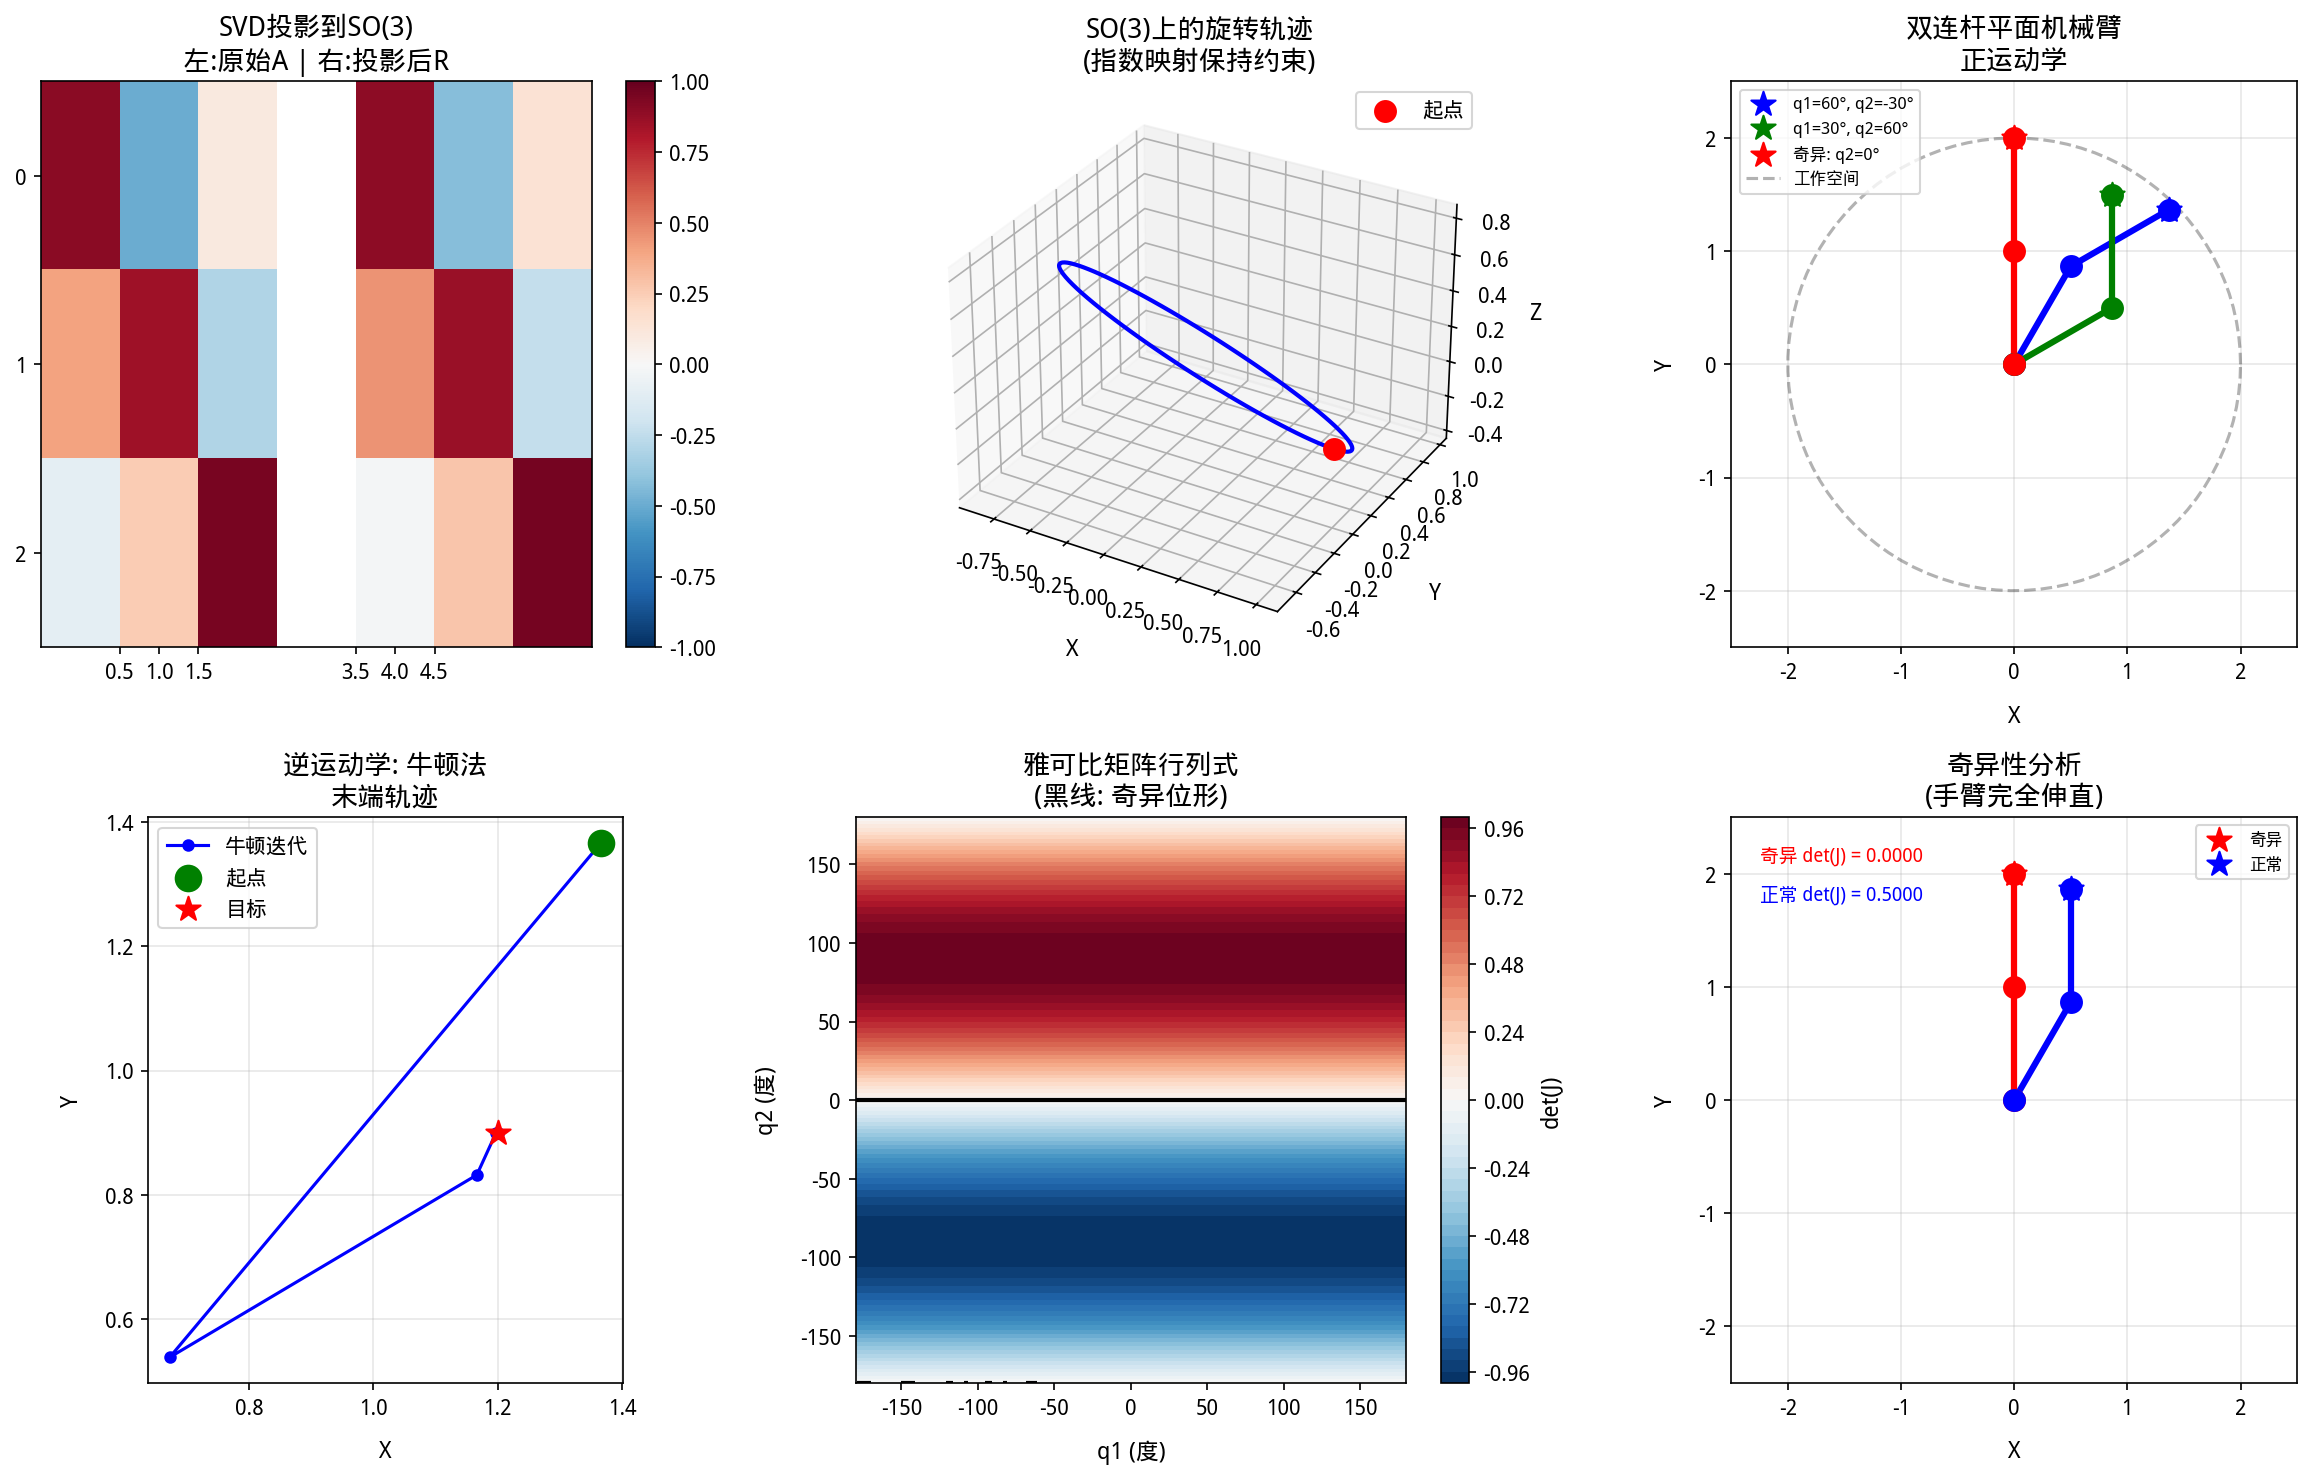
\includegraphics[width=0.98\textwidth]{figs/chap07_fig1.png}
\caption{机器人运动学与动力学演示。（1）SVD投影到SO(3)：将任意矩阵投影为有效旋转矩阵；（2）指数映射演示：在SO(3)流形上的正确旋转更新轨迹；（3）双连杆机械臂正运动学与工作空间；（4）牛顿法求解逆运动学的迭代收敛过程；（5）雅可比行列式热图，黑线标示奇异位形（$q_2 = 0, \pm\pi$）；（6）奇异性分析：手臂完全伸直时的奇异位形对比正常位形。代码验证：力传递结果$\tau = (-20, -10)$ Nm与书中一致。}
\label{fig:chap07_robotics}
\end{figure}

% ------------------------------------------------------------------------------------
\section{本章小结}

\begin{enumerate}
    \item \textbf{运动学}描述位置关系：正运动学 $x = f(q)$ 简单且唯一，逆运动学 $q = f^{-1}(x)$ 复杂且可能多解。
    
    \item \textbf{雅可比矩阵}是核心工具：$J$ 映射速度（$\dot{x} = J\dot{q}$），$J^\top$ 映射力（$\tau = J^\top F$）。这来自虚功原理。
    
    \item \textbf{奇异性}限制了机械臂的能力：在奇异位形，某些方向无法运动，某些方向力矩发散。
    
    \item \textbf{冗余}提供了额外自由度：零空间运动不影响末端，可用于次级目标（避障、远离限位等）。
    
    \item \textbf{动力学}来自拉格朗日方程：$M\ddot{q} + C\dot{q} + G = \tau$，把关节力矩与运动联系起来。
    
    \item \textbf{接触力}是拉格朗日乘子：互补条件 $\lambda \phi = 0$ 描述"接触才有力"，与线性规划的对偶理论一脉相承。
\end{enumerate}

\begin{unification}[title=$\lambda$ 在机器人学中的多重身份]
\begin{center}
\renewcommand{\arraystretch}{1.4}
\begin{tabular}{l|l|l}
\toprule
\textbf{场景} & \textbf{$\lambda$ 的含义} & \textbf{与优化的联系} \\
\midrule
逆运动学 & 末端约束力 & 等式约束的乘子 \\
关节限位 & 限位反力 & 不等式约束的乘子 \\
接触力 & 地面反作用力 & 互补约束的乘子 \\
闭链机构 & 环路内力 & 代数约束的乘子 \\
\bottomrule
\end{tabular}
\end{center}
\end{unification}

\begin{insightbox}
机器人学是约束优化最直接的工程应用。每一个关节限位、每一次接触、每一个任务目标，都对应着一个约束，而拉格朗日乘子 $\lambda$ 就是这些约束的"代言人"——它把抽象的几何限制转化为具体的物理力。

当你看到一个机械臂优雅地抓取物体，或者一个机器人稳健地行走，背后都是这些数学在默默工作。
\end{insightbox}

% ------------------------------------------------------------------------------------
\section{习题}

\paragraph{计算题}
\begin{enumerate}
    \item 双连杆机械臂，$L_1 = 1.2$ m，$L_2 = 0.8$ m。
    \begin{enumerate}
        \item 计算 $q_1 = 30°$，$q_2 = 45°$ 时的末端位置 $(x, y)$
        \item 计算此时的雅可比矩阵 $J$
        \item 若末端受力 $F = (5, 3)^\top$ N，求所需关节力矩 $\tau$
    \end{enumerate}
    
    \item 同上机械臂，目标末端位置为 $(1.5, 0.8)$。
    \begin{enumerate}
        \item 检验该目标是否在工作空间内
        \item 用几何方法求解逆运动学（提示：用余弦定理）
        \item 画出两个解对应的机械臂构型
    \end{enumerate}
    
    \item 单摆系统，质量 $m = 2$ kg，长度 $L = 0.5$ m。
    \begin{enumerate}
        \item 写出动能 $T$ 和势能 $V$ 的表达式
        \item 用拉格朗日方程推导运动方程
        \item 当摆角 $q = 60°$ 时，需要多大力矩才能保持静止？
    \end{enumerate}
\end{enumerate}

\paragraph{证明题}
\begin{enumerate}
    \setcounter{enumi}{3}
    \item 证明雅可比转置定理：若末端速度 $\dot{x} = J\dot{q}$，则关节力矩与末端力的关系为 $\tau = J^\top F$。（提示：从虚功原理 $\delta W = \tau^\top \delta q = F^\top \delta x$ 出发）
    
    \item 证明：当 $q_2 = 0$（手臂伸直）时，双连杆机械臂的雅可比矩阵奇异。从物理角度解释这意味着什么。
    
    \item 设 $J^\dagger = J^\top(JJ^\top)^{-1}$ 是雅可比矩阵的伪逆。证明：
    \begin{enumerate}
        \item $JJ^\dagger = I$（左逆性质）
        \item $(I - J^\dagger J)$ 是投影到零空间的投影矩阵，即 $J(I - J^\dagger J) = 0$
    \end{enumerate}
\end{enumerate}

\paragraph{编程题}
\begin{enumerate}
    \setcounter{enumi}{6}
    \item 实现双连杆机械臂的正运动学和雅可比计算，并可视化：
    \begin{enumerate}
        \item 给定关节角轨迹 $q(t)$，画出末端轨迹
        \item 在同一图中显示机械臂的运动过程（动画或多帧叠加）
    \end{enumerate}
    
    \item 实现牛顿迭代法求解逆运动学：
    \begin{enumerate}
        \item 给定目标位置，从不同初值出发，观察收敛到不同解的情况
        \item 处理奇异位形附近的数值稳定性（阻尼最小二乘法）
        \item 让末端沿直线轨迹运动，计算对应的关节轨迹
    \end{enumerate}
    
    \item （挑战）实现三连杆冗余机械臂（$n=3$，$m=2$）的逆运动学：
    \begin{enumerate}
        \item 实现基于伪逆的逆运动学
        \item 利用零空间实现次级目标：远离关节限位
        \item 可视化零空间运动：固定末端，观察肘关节的运动范围
    \end{enumerate}
\end{enumerate}

\paragraph{思考题}
\begin{enumerate}
    \setcounter{enumi}{9}
    \item 人的手臂有7个自由度，而控制手掌位置和朝向只需要6个自由度。这个"多余"的自由度在日常生活中有什么作用？举两个具体例子。
    
    \item 为什么工业机器人大多采用6自由度设计，而不是更多？从成本、控制复杂度、可靠性等角度分析。
    
    \item 接触力学中的互补条件 $\lambda \cdot \phi = 0$ 与线性规划中的互补松弛条件有何联系？从"稀缺资源才有价格"的角度解释接触力的物理意义。
    
    \item 机器人行走时，脚与地面的接触力是如何让机器人前进的？如果地面完全光滑（无摩擦），机器人还能行走吗？为什么？
    
    \item 比较牛顿-欧拉法和拉格朗日法计算机器人动力学的优缺点。在什么情况下你会选择哪种方法？
\end{enumerate}



% ====================================================================================
% ====================================================================================
% ====================================================================================
\section*{扩展阅读：从旋转矩阵到三维重建}
\addcontentsline{toc}{section}{扩展阅读：从旋转矩阵到三维重建}
% ====================================================================================

在本章中，我们用齐次变换矩阵 $T = \begin{bmatrix} R & p \\ 0 & 1 \end{bmatrix}$ 来描述机器人的位姿。位置向量 $p$ 很好处理——三个实数，想怎么改就怎么改。但旋转矩阵 $R$ 就没那么"自由"了：它必须满足 $R^\top R = I$ 和 $\det(R) = 1$。

这让我们想起了一个老朋友：\textbf{约束优化}。

等等，$R^\top R = I$ 不就是等式约束吗？我们有拉格朗日乘子法啊！

没错。这一节，我们就从拉格朗日乘子法出发，看看它如何自然地引出一个优美的数学结构——\textbf{李群与李代数}。最后，我们会用这些工具来理解一个非常酷的应用：\textbf{高斯泼溅（Gaussian Splatting）}——2023年爆火的三维重建技术。

%------------------------------------------------------------------------------
\subsection*{热身：单位向量的约束优化}
%------------------------------------------------------------------------------

在处理旋转矩阵之前，让我们先看一个更简单的例子：\textbf{单位向量}。

\paragraph{问题：在单位圆上找最近点}

假设你有一个二维向量 $v_0 = (2, 1)$，你想找一个\textbf{单位向量} $v$（满足 $\|v\| = 1$），使得 $v$ 尽可能接近 $v_0$。

\begin{figure}[h]
\centering
\begin{tikzpicture}[scale=1.2]
    % 坐标轴
    \draw[->] (-1.5, 0) -- (2.5, 0) node[right] {$x$};
    \draw[->] (0, -1.5) -- (0, 1.8) node[above] {$y$};
    
    % 单位圆
    \draw[thick, blue] (0,0) circle (1);
    \node[blue] at (1.3, -1) {单位圆 $\|v\|=1$};
    
    % 目标点
    \fill[red] (2, 1) circle (3pt);
    \node[red, right] at (2.1, 1) {$v_0 = (2, 1)$};
    
    % 最优解
    \fill[green!60!black] ({2/sqrt(5)}, {1/sqrt(5)}) circle (3pt);
    \node[green!60!black, above right] at ({2/sqrt(5)}, {1/sqrt(5)}) {$v^*$};
    
    % 连线
    \draw[dashed, gray] (0, 0) -- (2, 1);
    \draw[->, thick, green!60!black] (0, 0) -- ({2/sqrt(5)}, {1/sqrt(5)});
\end{tikzpicture}
\caption{在单位圆上找离 $v_0$ 最近的点}
\end{figure}

用数学语言写出来：
\begin{equation}
\min_{v \in \mathbb{R}^2} \frac{1}{2}\|v - v_0\|^2 \quad \st \quad \|v\|^2 - 1 = 0
\end{equation}

\paragraph{用拉格朗日乘子法求解}

构造拉格朗日函数：
\begin{equation}
\mathcal{L}(v, \lambda) = \frac{1}{2}\|v - v_0\|^2 + \lambda (\|v\|^2 - 1)
\end{equation}

对 $v$ 求导：
\begin{equation}
\nabla_v \mathcal{L} = (v - v_0) + 2\lambda v = 0
\end{equation}

整理得：
\begin{equation}
v = \frac{v_0}{1 + 2\lambda}
\end{equation}

代入约束 $\|v\| = 1$：
\begin{equation}
\left\| \frac{v_0}{1 + 2\lambda} \right\| = 1 \quad \Rightarrow \quad |1 + 2\lambda| = \|v_0\|
\end{equation}

因为 $\|v_0\| = \sqrt{5} > 1$，我们取 $1 + 2\lambda = \sqrt{5}$（另一个解对应最远点）。

所以：
\begin{equation}
v^* = \frac{v_0}{\|v_0\|} = \frac{(2, 1)}{\sqrt{5}} = \left( \frac{2}{\sqrt{5}}, \frac{1}{\sqrt{5}} \right)
\end{equation}

\textbf{结论}：最优解就是把 $v_0$ 归一化！这个结果很直观——离 $v_0$ 最近的单位向量，就是 $v_0$ 方向上的那个单位向量。

\paragraph{乘子 $\lambda$ 的意义}

回忆一下，拉格朗日乘子表示"约束的价格"。这里 $\lambda = \frac{\sqrt{5} - 1}{2} \approx 0.618$。

如果我们把约束稍微放松一点（允许 $\|v\|^2 \leq 1 + \epsilon$），目标函数会减少大约 $\lambda \cdot \epsilon$。

\begin{insightbox}
\textbf{这个简单例子告诉我们什么？}

\begin{enumerate}
    \item 约束 $\|v\| = 1$ 把优化限制在一个\textbf{圆}上
    \item 拉格朗日乘子法可以处理这种约束
    \item 最优解是 $v_0$ 在圆上的\textbf{投影}
\end{enumerate}

接下来，我们把同样的思路用到旋转矩阵上。
\end{insightbox}

%------------------------------------------------------------------------------
\subsection*{旋转矩阵：9个变量，6个约束}
%------------------------------------------------------------------------------

现在让我们来看旋转矩阵。一个 $3 \times 3$ 的旋转矩阵 $R$ 必须满足：
\begin{equation}
R^\top R = I, \quad \det(R) = 1
\end{equation}

满足这两个条件的所有矩阵构成一个集合，数学家给它起了一个名字：

\begin{definition}[特殊正交群 $SO(3)$]
\textbf{特殊正交群}（Special Orthogonal Group）定义为：
\begin{equation}
SO(3) = \{ R \in \mathbb{R}^{3 \times 3} : R^\top R = I, \, \det(R) = 1 \}
\end{equation}

\begin{itemize}
    \item \textbf{正交}（Orthogonal）：$R^\top R = I$，即 $R$ 的列向量相互垂直且长度为1
    \item \textbf{特殊}（Special）：$\det(R) = 1$，排除了镜像反射（镜像反射的行列式是 $-1$）
    \item \textbf{群}（Group）：旋转可以复合（矩阵乘法）、可以求逆（$R^{-1} = R^\top$），满足群的公理
\end{itemize}

类似地，二维旋转构成 $SO(2)$，$n$ 维旋转构成 $SO(n)$。
\end{definition}

\paragraph{约束有多少个？}

$R^\top R = I$ 是一个 $3 \times 3$ 的矩阵方程。但因为 $R^\top R$ 是对称矩阵，只有6个独立的方程：
\begin{itemize}
    \item 3个对角元 = 1：每列的长度是1
    \item 3个非对角元 = 0：列与列相互垂直
\end{itemize}

$\det(R) = 1$ 看起来是第7个约束，但实际上，一旦 $R^\top R = I$，就有 $\det(R) = \pm 1$。我们只是在两个"分支"中选择 $+1$ 那个。

所以：\textbf{9个变量，6个约束，3个自由度}。

\begin{figure}[h]
\centering
\begin{tikzpicture}[scale=0.85]
    % 9维空间
    \draw[thick, fill=blue!5] (0,0) ellipse (4 and 2.5);
    \node at (0, 2) {$\mathbb{R}^{3 \times 3}$（所有 $3\times 3$ 矩阵，9维）};
    
    % SO(3)
    \draw[thick, fill=red!20] (0, -0.3) ellipse (1.5 and 1);
    \node at (0, -0.3) {$SO(3)$};
    \node at (0, -1) {\small （旋转矩阵，3维曲面）};
    
    % 约束
    \draw[->, thick] (3, 1) -- (1.5, 0.2);
    \node[align=left, right] at (3, 1) {6个约束\\把9维"压缩"到3维};
\end{tikzpicture}
\caption{$SO(3)$ 是9维矩阵空间中的一个3维曲面}
\end{figure}

这3个自由度对应什么？就是我们熟悉的\textbf{三个旋转角}——比如绕 $x$、$y$、$z$ 轴的欧拉角。

\paragraph{问题：找最近的旋转矩阵}

假设你有一个"差不多是旋转矩阵"的矩阵 $A$（比如从噪声数据估计出来的），你想找一个\textbf{真正的旋转矩阵} $R$，使得 $R$ 尽可能接近 $A$。

\begin{equation}
\min_{R \in \mathbb{R}^{3 \times 3}} \|R - A\|_F^2 \quad \st \quad R^\top R = I, \quad \det(R) = 1
\end{equation}

这里 $\|\cdot\|_F$ 是 Frobenius 范数（矩阵元素的平方和再开根）。

\paragraph{拉格朗日函数}

约束 $R^\top R = I$ 有6个独立方程，需要引入一个\textbf{对称矩阵} $\Lambda \in \mathbb{R}^{3 \times 3}$ 作为乘子：

\begin{equation}
\mathcal{L}(R, \Lambda) = \|R - A\|_F^2 + \langle \Lambda, R^\top R - I \rangle
\end{equation}

其中 $\langle \Lambda, M \rangle = \tr(\Lambda^\top M)$ 是矩阵内积。

对 $R$ 求导（这需要一点矩阵微积分）：
\begin{equation}
\nabla_R \mathcal{L} = 2(R - A) + 2R\Lambda = 0
\end{equation}

整理：
\begin{equation}
R(I + \Lambda) = A
\end{equation}

这个方程告诉我们 $R$ 和 $A$ 的关系，但还需要代入约束来求解 $\Lambda$。

\paragraph{SVD 给出答案}

对 $A$ 做奇异值分解（SVD）：$A = U \Sigma V^\top$。

可以证明，最优解是：
\begin{equation}
R^* = U V^\top
\end{equation}

（如果 $\det(UV^\top) = -1$，需要翻转 $V$ 的一列。）

\begin{physicalmeaning}
\textbf{投影到 $SO(3)$ 上}

就像单位向量的例子中，最优解是"投影"到约束集合上一样：

最接近 $A$ 的旋转矩阵 = $A$ 在 $SO(3)$ 上的\textbf{投影}

SVD 自动帮我们完成了这个投影！
\end{physicalmeaning}

\begin{lstlisting}[style=teaching, language=Python]
import numpy as np

# 一个"有噪声"的矩阵
A = np.array([
    [0.9, -0.5, 0.1],
    [0.4, 0.85, -0.3],
    [-0.1, 0.25, 0.95]
])

print("A 不是旋转矩阵：")
print("A^T @ A =\n", np.round(A.T @ A, 3))
print("det(A) =", np.round(np.linalg.det(A), 3))

# 用 SVD 投影到 SO(3)
U, S, Vt = np.linalg.svd(A)
R = U @ Vt

# 确保 det = +1
if np.linalg.det(R) < 0:
    Vt[-1, :] *= -1
    R = U @ Vt

print("\nR 是旋转矩阵：")
print("R^T @ R =\n", np.round(R.T @ R, 3))
print("det(R) =", np.round(np.linalg.det(R), 3))
\end{lstlisting}

%------------------------------------------------------------------------------
\subsection*{约束的"隐藏结构"：为什么反对称矩阵会出现？}
%------------------------------------------------------------------------------

现在让我们换一个角度，看看约束 $R^\top R = I$ 隐藏着什么数学结构。

\paragraph{问旋转矩阵的"邻居"长什么样}

假设 $R$ 是一个旋转矩阵，我们想知道：$R$ 附近还有哪些旋转矩阵？

设 $R(\epsilon) = R + \epsilon \cdot \Delta R$ 是一个"稍微偏离 $R$"的矩阵。如果 $R(\epsilon)$ 也要是旋转矩阵，必须满足：
\begin{equation}
R(\epsilon)^\top R(\epsilon) = I
\end{equation}

展开：
\begin{equation}
(R + \epsilon \Delta R)^\top (R + \epsilon \Delta R) = R^\top R + \epsilon(R^\top \Delta R + \Delta R^\top R) + O(\epsilon^2) = I
\end{equation}

因为 $R^\top R = I$，一阶项必须为零：
\begin{equation}
R^\top \Delta R + \Delta R^\top R = 0
\end{equation}

设 $\Omega = R^\top \Delta R$，则上式变成：
\begin{equation}
\Omega + \Omega^\top = 0
\end{equation}

这说明 $\Omega$ 是\textbf{反对称矩阵}！

\begin{keyformula}[title=旋转矩阵的"合法扰动"]
如果 $R$ 是旋转矩阵，那么 $R$ 的"合法扰动方向" $\Delta R$ 必须满足：
\begin{equation}
R^\top \Delta R = \Omega \quad \text{其中 } \Omega^\top = -\Omega
\end{equation}

等价地：$\Delta R = R \Omega$，其中 $\Omega$ 是任意反对称矩阵。
\end{keyformula}

\paragraph{反对称矩阵有什么特点？}

一个 $3 \times 3$ 反对称矩阵长这样：
\begin{equation}
\Omega = \begin{bmatrix} 0 & -\omega_3 & \omega_2 \\ \omega_3 & 0 & -\omega_1 \\ -\omega_2 & \omega_1 & 0 \end{bmatrix}
\end{equation}

只有\textbf{3个自由参数} $(\omega_1, \omega_2, \omega_3)$——正好对应旋转矩阵的3个自由度！

我们引入一个方便的记号：

\begin{definition}[反对称矩阵与向量的对应]
对于向量 
\[
\omega = 
(\omega_1,\; \omega_2,\; \omega_3)^\top \in \mathbb{R}^3,
\]
定义其对应的反对称矩阵为：
\[
[\omega]_\times 
=
\begin{bmatrix}
0        & -\omega_3 & \ \omega_2 \\
\omega_3 & 0         & -\omega_1  \\
-\omega_2& \omega_1  & 0
\end{bmatrix}.
\]


这个记号叫做 \textbf{hat operator}（帽子算子），因为有些文献写成 $\hat{\omega}$。

它有一个非常漂亮的性质：
\begin{equation}
[\omega]_\times v = \omega \times v \quad \text{（矩阵乘法 = 叉积！）}
\end{equation}

也就是说，反对称矩阵左乘一个向量，等价于用 $\omega$ 对这个向量做叉积。
\end{definition}

这个向量 $\omega = (\omega_1, \omega_2, \omega_3)^\top$ 有一个物理意义：\textbf{角速度}。

\begin{physicalmeaning}
想象一个刚体正在旋转。在某一时刻，它的姿态是 $R$，角速度是 $\omega$。

那么姿态的变化率是：
\begin{equation}
\dot{R} = R \cdot [\omega]_\times
\end{equation}

其中 $[\omega]_\times$ 就是由 $\omega$ 构成的反对称矩阵。

\textbf{约束 $R^\top R = I$ 自动保证了这个关系！}
\end{physicalmeaning}

%------------------------------------------------------------------------------
\subsection*{离散化：从连续旋转到旋转更新}
%------------------------------------------------------------------------------

在实际计算中，我们经常需要"更新"一个旋转矩阵。比如：

\begin{itemize}
    \item 机器人每隔 $\Delta t$ 测量一次角速度 $\omega$，需要更新姿态 $R$
    \item 优化算法计算出一个"旋转修正量"，需要应用到当前估计上
\end{itemize}

\paragraph{错误的更新方式}

如果你直接这样更新：
\begin{equation}
R_{new} = R_{old} + \Delta t \cdot \dot{R} = R_{old} + \Delta t \cdot R_{old} [\omega]_\times
\end{equation}

问题是：$R_{new}$ 不再满足 $R^\top R = I$！

\begin{lstlisting}[style=teaching, language=Python]
import numpy as np

def skew(w):
    return np.array([[0, -w[2], w[1]], 
                     [w[2], 0, -w[0]], 
                     [-w[1], w[0], 0]])

R = np.eye(3)  # 初始姿态
omega = np.array([0.1, 0.2, 0.3])  # 角速度
dt = 0.1

# 错误的欧拉更新
R_wrong = R + dt * R @ skew(omega)

print("错误更新后：")
print("R^T @ R =\n", np.round(R_wrong.T @ R_wrong, 4))
# 不是单位阵！
\end{lstlisting}

\paragraph{正确的更新方式：指数映射}

正确的做法是使用\textbf{指数映射}：
\begin{equation}
R_{new} = R_{old} \cdot \exp([\omega \cdot \Delta t]_\times)
\end{equation}

这里的 $\exp$ 是什么意思？它是\textbf{矩阵指数}（matrix exponential），定义方式和普通指数函数的泰勒展开完全类似：

\begin{definition}[矩阵指数]
对于任意方阵 $A$，其矩阵指数定义为：
\begin{equation}
\exp(A) = I + A + \frac{A^2}{2!} + \frac{A^3}{3!} + \cdots = \sum_{k=0}^{\infty} \frac{A^k}{k!}
\end{equation}

这个级数对任意方阵都收敛。当 $A$ 是 $1 \times 1$ 矩阵（即普通数字）时，就退化为普通的 $e^a$。
\end{definition}

对于反对称矩阵 $[\omega]_\times$，这个无穷级数有一个漂亮的闭式解：

\begin{keytheorem}[title=罗德里格斯公式（Rodrigues' Formula）]
设 $\theta = \|\omega\|$，$\hat{\omega} = \omega / \theta$。则：
\begin{equation}
\exp([\omega]_\times) = I + \sin\theta \cdot [\hat{\omega}]_\times + (1 - \cos\theta) \cdot [\hat{\omega}]_\times^2
\end{equation}

物理意义：绕轴 $\hat{\omega}$ 旋转角度 $\theta$。
\end{keytheorem}

\begin{lstlisting}[style=teaching, language=Python]
def exp_so3(omega):
    """指数映射：反对称矩阵 -> 旋转矩阵"""
    theta = np.linalg.norm(omega)
    if theta < 1e-10:
        return np.eye(3)
    w_hat = omega / theta
    K = skew(w_hat)
    return np.eye(3) + np.sin(theta) * K + (1 - np.cos(theta)) * K @ K

# 正确的更新
delta_R = exp_so3(omega * dt)
R_correct = R @ delta_R

print("正确更新后：")
print("R^T @ R =\n", np.round(R_correct.T @ R_correct, 4))
# 是单位阵！
\end{lstlisting}

\paragraph{为什么这样做是对的？}

关键观察：$\exp([\omega]_\times)$ \textbf{一定是}旋转矩阵（无论 $\omega$ 是什么）！

而且，两个旋转矩阵的乘积也一定是旋转矩阵。所以 $R_{old} \cdot \exp([\cdot]_\times)$ 一定在 $SO(3)$ 上。

这就是\textbf{流形上优化}的核心思想：不要直接在矩阵空间里加减，而是用"旋转乘旋转"的方式更新。

%------------------------------------------------------------------------------
\subsection*{李群与李代数：给这些结构起个名字}
%------------------------------------------------------------------------------

我们刚才发现的这些结构，数学家们早就研究过了，还给它们起了名字。

\begin{definition}[李群与李代数（直观版）]

\begin{itemize}
    \item \textbf{李群}：一个既是"群"又是"光滑曲面"的数学对象。"群"意味着可以做乘法和求逆；"光滑曲面"意味着可以做微积分。
    
    \item \textbf{李代数}：李群在单位元处的"切空间"。它是一个普通的向量空间，可以自由地做加减法。
\end{itemize}
\end{definition}

对于旋转矩阵：
\begin{center}
\renewcommand{\arraystretch}{1.4}
\begin{tabular}{c|c|c|c}
\toprule
\textbf{李群} & \textbf{元素} & \textbf{李代数} & \textbf{元素} \\
\midrule
$SO(3)$ & 旋转矩阵 $R$ & $\mathfrak{so}(3)$ & 反对称矩阵 $[\omega]_\times$ \\
 & $R^\top R = I, \det R = 1$ & & 或等价地，向量 $\omega \in \mathbb{R}^3$ \\
\bottomrule
\end{tabular}
\end{center}

指数映射和对数映射在两者之间建立联系：
\begin{equation}
\exp: \mathfrak{so}(3) \to SO(3), \quad \log: SO(3) \to \mathfrak{so}(3)
\end{equation}

\begin{figure}[h]
\centering
\begin{tikzpicture}[scale=1.0]
    % 李群
    \draw[thick, fill=blue!10] (0,0) ellipse (2.5 and 1.5);
    \node at (0, 0) {$SO(3)$};
    \node at (0, -0.5) {\small 旋转矩阵};
    
    % 李代数
    \draw[thick, fill=green!10] (7,0) ellipse (2.5 and 1.5);
    \node at (7, 0) {$\mathfrak{so}(3) \cong \mathbb{R}^3$};
    \node at (7, -0.5) {\small 角速度向量};
    
    % 箭头
    \draw[->, thick, red] (2.5, 0.5) .. controls (4, 1.2) and (5, 1.2) .. (4.5, 0.5);
    \node[red, above] at (3.5, 1.2) {$\log$};
    
    \draw[->, thick, blue] (4.5, -0.5) .. controls (5, -1.2) and (4, -1.2) .. (2.5, -0.5);
    \node[blue, below] at (3.5, -1.2) {$\exp$};
    
    % 说明
    \node[align=center] at (3.5, -2.5) {
        在李代数中计算（普通向量运算）\\
        用 $\exp$ 映射回李群
    };
\end{tikzpicture}
\caption{李群与李代数的关系}
\end{figure}

\paragraph{为什么这个框架有用？}

\begin{enumerate}
    \item \textbf{最小参数化}：$\omega \in \mathbb{R}^3$ 恰好有3个参数，没有冗余
    \item \textbf{无约束优化}：在 $\mathbb{R}^3$ 中优化 $\omega$，不需要处理 $R^\top R = I$
    \item \textbf{数值稳定}：用 $\exp$ 映射回去，自动保证结果是旋转矩阵
\end{enumerate}

%------------------------------------------------------------------------------
\subsection*{$SE(3)$：位置 + 姿态一起处理}
%------------------------------------------------------------------------------

在机器人学中，我们经常需要同时描述位置和姿态——这就是\textbf{位姿}（pose）。

位姿可以用齐次变换矩阵表示，所有这样的矩阵构成另一个重要的群：

\begin{definition}[特殊欧氏群 $SE(3)$]
\textbf{特殊欧氏群}（Special Euclidean Group）定义为：
\begin{equation}
SE(3) = \left\{ T = \begin{bmatrix} R & p \\ 0 & 1 \end{bmatrix} : R \in SO(3), \, p \in \mathbb{R}^3 \right\}
\end{equation}

\begin{itemize}
    \item $R \in SO(3)$：旋转部分（3个自由度）
    \item $p \in \mathbb{R}^3$：平移部分（3个自由度）
    \item 总共 \textbf{6个自由度}
\end{itemize}

$SE(3)$ 描述了三维空间中刚体的所有可能位姿。类似地，$SE(2)$ 描述平面刚体运动（3个自由度）。
\end{definition}

$SE(3)$ 也是一个李群！它的李代数是 $\mathfrak{se}(3)$，包含6个参数：
\begin{equation}
\xi = \begin{pmatrix} v \\ \omega \end{pmatrix} \in \mathbb{R}^6
\end{equation}

\begin{itemize}
    \item $v \in \mathbb{R}^3$：线速度
    \item $\omega \in \mathbb{R}^3$：角速度
\end{itemize}

这个6维向量叫做\textbf{旋量}（twist），它描述了刚体的瞬时运动。

%------------------------------------------------------------------------------
\subsection*{应用：相机位姿估计与SLAM}
%------------------------------------------------------------------------------

现在让我们看看这些数学工具在实际中怎么用。

\paragraph{问题：从照片恢复相机位置}

假设你用手机拍了几张照片，想知道每张照片是在哪里、朝哪个方向拍的。这就是\textbf{相机位姿估计}问题。

\begin{figure}[h]
\centering
\begin{tikzpicture}[scale=0.9]
    % 相机轨迹
    \foreach \i/\x/\y/\angle in {1/0/0/30, 2/2/0.8/15, 3/4/1.2/0, 4/6/0.8/-20} {
        % 相机图标
        \begin{scope}[shift={(\x, \y)}, rotate=\angle]
            \draw[thick, fill=gray!30] (-0.2, -0.15) rectangle (0.2, 0.15);
            \draw[thick] (0.2, 0) -- (0.5, 0.2) -- (0.5, -0.2) -- cycle;
        \end{scope}
        \node[below] at (\x, \y-0.4) {\small $T_\i$};
    }
    
    % 3D点
    \foreach \x/\y in {1/2.5, 3/2.8, 5/2.2} {
        \fill[red] (\x, \y) circle (3pt);
    }
    \node[red] at (3, 3.3) {\small 场景中的3D点};
    
    % 观测线
    \draw[dashed, gray, opacity=0.5] (0, 0) -- (1, 2.5);
    \draw[dashed, gray, opacity=0.5] (2, 0.8) -- (1, 2.5);
    \draw[dashed, gray, opacity=0.5] (2, 0.8) -- (3, 2.8);
    \draw[dashed, gray, opacity=0.5] (4, 1.2) -- (3, 2.8);
    \draw[dashed, gray, opacity=0.5] (4, 1.2) -- (5, 2.2);
    \draw[dashed, gray, opacity=0.5] (6, 0.8) -- (5, 2.2);
\end{tikzpicture}
\caption{相机位姿估计：从多张照片恢复相机轨迹}
\end{figure}

\paragraph{优化问题的建立}

设第 $i$ 个相机的位姿是 $T_i \in SE(3)$，第 $j$ 个3D点在世界坐标系中的坐标是 $p_j \in \mathbb{R}^3$。

如果相机 $i$ 看到了点 $j$，在图像上的像素坐标是 $z_{ij} \in \mathbb{R}^2$。根据针孔相机模型，理论上应该有：
\begin{equation}
z_{ij} \approx \pi(T_i^{-1} \cdot p_j)
\end{equation}

这里 $\pi: \mathbb{R}^3 \to \mathbb{R}^2$ 是\textbf{相机投影函数}，它把相机坐标系下的3D点投影到2D图像平面：
\begin{equation}
\pi\begin{pmatrix} X \\ Y \\ Z \end{pmatrix} = \begin{pmatrix} f_x \cdot X/Z + c_x \\ f_y \cdot Y/Z + c_y \end{pmatrix}
\end{equation}
其中 $f_x, f_y$ 是焦距（以像素为单位），$(c_x, c_y)$ 是图像中心。这些参数称为\textbf{相机内参}，可以通过标定获得。

优化目标是最小化\textbf{重投影误差}——理论投影位置和实际观测位置的差距：
\begin{equation}
\min_{T_1, \ldots, T_n, p_1, \ldots, p_m} \sum_{(i,j) \in \mathcal{O}} \| z_{ij} - \pi(T_i^{-1} p_j) \|^2
\end{equation}
其中 $\mathcal{O}$ 是所有"相机 $i$ 看到点 $j$"的观测对集合。

\paragraph{用李代数参数化}

直接优化 $T_i$ 的16个元素会遇到约束问题（必须保持 $R^\top R = I$）。正确的做法是用李代数参数化。

首先，我们需要把6维向量变成 $4 \times 4$ 矩阵。类似于 $[\omega]_\times$ 把 $\mathbb{R}^3$ 映射到反对称矩阵，我们定义 $SE(3)$ 的"帽子算子"：

\begin{definition}[$SE(3)$ 的 $\wedge$（wedge）算子]
对于 $\xi = (v_1, v_2, v_3, \omega_1, \omega_2, \omega_3)^\top \in \mathbb{R}^6$，定义：
\begin{equation}
\xi^\wedge = \begin{bmatrix} [\omega]_\times & v \\ 0 & 0 \end{bmatrix} = 
\begin{bmatrix} 
0 & -\omega_3 & \omega_2 & v_1 \\
\omega_3 & 0 & -\omega_1 & v_2 \\
-\omega_2 & \omega_1 & 0 & v_3 \\
0 & 0 & 0 & 0
\end{bmatrix} \in \mathbb{R}^{4 \times 4}
\end{equation}
其中 $v = (v_1, v_2, v_3)^\top$ 对应平移，$\omega = (\omega_1, \omega_2, \omega_3)^\top$ 对应旋转。

这是李代数 $\mathfrak{se}(3)$ 中的元素。
\end{definition}

现在，对每个位姿 $T_i$，在当前估计值 $\bar{T}_i$ 附近用李代数参数化：
\begin{equation}
T_i = \bar{T}_i \cdot \exp(\xi_i^\wedge)
\end{equation}
其中 $\xi_i \in \mathbb{R}^6$ 是要优化的小量，$\exp(\xi_i^\wedge)$ 通过矩阵指数把它变成 $SE(3)$ 中的元素。

现在，优化变量变成了 $\xi_1, \ldots, \xi_n \in \mathbb{R}^6$ 和 $p_1, \ldots, p_m \in \mathbb{R}^3$——全都是普通的实数向量，没有任何约束，可以用标准的非线性最小二乘方法（如高斯-牛顿法、LM算法）求解！

这就是\textbf{视觉SLAM}（Simultaneous Localization and Mapping，即时定位与地图构建）的核心技术。你手机上的AR应用、自动驾驶汽车的定位系统，都在用这个原理。


%------------------------------------------------------------------------------
%------------------------------------------------------------------------------
\subsection*{本节小结}
%------------------------------------------------------------------------------

\begin{enumerate}
    \item \textbf{旋转矩阵的约束} $R^\top R = I$ 可以用拉格朗日乘子法处理，最优投影由SVD给出。
    
    \item \textbf{约束的结构}揭示了深层数学：合法的扰动方向必须是反对称矩阵，这自然引出了李代数。
    
    \item \textbf{李群 $SO(3)$} 是旋转矩阵的集合，\textbf{李代数 $\mathfrak{so}(3)$} 是反对称矩阵（或等价地，$\mathbb{R}^3$ 向量）。
    
    \item \textbf{指数映射}把李代数元素变成李群元素，保证更新后仍然满足约束。
    
    \item \textbf{实际应用}：视觉SLAM用李代数参数化相机位姿
\end{enumerate}

\begin{remark}
从拉格朗日乘子法到李群李代数，我们看到了同一个主题的不断深化：\textbf{如何优雅地处理约束}。

拉格朗日乘子法说：把约束编码到目标函数里。

李群理论说：选择一个参数化，让约束\textbf{自动满足}。

两种思路各有优势，在实际问题中常常结合使用。
\end{remark}

%--------------------------------------------------------------------------  % 第7章：机器人运动学与动力学
% ====================================================================================
\chapter{轨迹优化：让机器人优雅地运动}
% ====================================================================================

\section*{引言：火箭是怎么知道该怎么飞的？}

2015年12月21日，SpaceX的猎鹰9号火箭在发射后成功返回着陆——这是人类历史上第一次轨道级火箭的垂直回收。火箭在返回过程中需要精确控制发动机推力和姿态，才能稳稳降落在只有足球场大小的着陆平台上。
\storynote{Lev Pontryagin}{庞特里亚金（1908--1988），苏联数学家，14岁因煤油炉爆炸双目失明，靠母亲为他朗读论文完成研究。1955年他带领几位学生转向工程问题，为苏联空军研究"最短时间拦截"，1956年提出最大值原理——本章的伴随方程正是它的核心。}

\begin{figure}[htbp]
\centering
\begin{tikzpicture}[scale=0.8]
    % 火箭轨迹
    \draw[thick, blue, ->] (0, 6) to[out=-60, in=120] (2, 4) to[out=-60, in=150] (4, 2) to[out=-30, in=90] (5, 0);
    
    % 火箭（简化）
    \draw[fill=gray!30] (4.8, 0.5) -- (5, 1.5) -- (5.2, 0.5) -- cycle;
    \draw[fill=orange] (4.9, 0.3) -- (5, 0.5) -- (5.1, 0.3) -- cycle;
    
    % 着陆平台
    \fill[brown!50] (4, 0) rectangle (6, -0.2);
    \node at (5, -0.5) {\small 着陆平台};
    
    % 标注
    \node[blue] at (1, 5) {返回轨迹};
    \draw[->, red, thick] (4.5, 1.5) -- (4.5, 2.2);
    \node[red, right] at (4.5, 2) {\small 推力};
    
    % 问题
    \node[align=left] at (8, 3) {每一时刻该用\\多大推力？\\什么方向？};
\end{tikzpicture}
\caption{火箭返回着陆：一个复杂的轨迹优化问题}
\end{figure}

这就是\textbf{轨迹优化}问题：给定起点和终点，找到一条最优的运动轨迹，同时满足物理定律（动力学约束）。

令人惊喜的是，这个看似复杂的问题，其数学本质仍然是我们熟悉的\textbf{约束优化}——只不过约束变成了微分方程！

\vspace{0.3cm}
\noindent\textit{为什么火箭"知道"现在该用多大推力？为什么规划一条轨迹要从终点倒着算？为什么自动驾驶每隔零点几秒就把整个计划推翻重来一遍？}

\begin{quote}
\textbf{本章目标}：把"让一个系统从这里最优地走到那里"写成约束优化问题——目标是累计代价，约束是每个时刻都必须成立的动力学方程 $\dot{x} = f(x, u)$。你会看到，第1章的乘子 $\lambda$ 在这里变成一条随时间变化的曲线 $\lambda(t)$，它必须从终点往回算，这就是伴随方程；而"规划多步、只走一步、再重新规划"的 MPC，则是把这个优化问题塞进反馈回路里的工程做法。读完本章，你已经握住了第9章反向传播和第10章贝尔曼方程的钥匙。
\end{quote}

\begin{tcolorbox}[colback=yellow!10, colframe=orange!80, title=本章的核心观点]
\textbf{轨迹优化 = 变分法 + 拉格朗日乘子法。}本章的问题就是第1章的拉格朗日乘子法，只是约束从"一个方程 $g(x) = 0$"变成了"每个时刻一个方程 $\dot{x}(t) = f(x(t), u(t))$"，于是乘子从一个数 $\lambda$ 变成一个函数 $\lambda(t)$。

\begin{center}
\renewcommand{\arraystretch}{1.3}
\small
\begin{tabular}{lll}
\toprule
 & \textbf{第1章} & \textbf{本章} \\
\midrule
变量 & 向量 $x \in \R^n$ & 轨迹 $x(t)$ 与控制 $u(t)$ \\
目标 & $f(x)$ & $J = \int_0^T L(x, u)\,dt + \phi(x(T))$ \\
约束 & $g(x) = 0$ & $f(x, u) - \dot{x} = 0$（每个 $t$ 一条） \\
乘子 & $\lambda$（一个数） & $\lambda(t)$（协态，一条曲线） \\
拉格朗日函数 & $f + \lambda^\top g$ & $\int_0^T [L + \lambda^\top (f - \dot{x})]\,dt$ \\
一阶条件 & $\nabla f + \lambda^\top \nabla g = 0$，$g = 0$ & $\partial H/\partial u = 0$，$\dot{\lambda} = -\partial H/\partial x$，$\dot{x} = f$ \\
$\lambda$ 的意义 & 影子价格 & 未来代价对当前状态的敏感度 \\
\bottomrule
\end{tabular}
\end{center}
离散化之后（$x_{k+1} = f(x_k, u_k)$），这张表的右栏就变成第9章神经网络那张表的左栏。
\end{tcolorbox}

\begin{tcolorbox}[colback=green!5, colframe=green!60!black, title=学完这章，你将能够...]
\begin{itemize}
    \item 把"最省力移动物体"等问题写成最优控制形式
    \item 推导并求解简单系统的伴随方程
    \item 用直接法（离散化）数值求解轨迹优化问题
    \item 理解反向传播与伴随方法的数学联系
    \item 分析火箭着陆、机器人行走等实际案例
\end{itemize}
\end{tcolorbox}

% ------------------------------------------------------------------------------------
\section{从最简单的问题开始}

\subsection{问题：最省力地移动一个物体}

考虑一个质量为 $m$ 的物体在一维直线上运动。初始时刻 $t=0$ 在原点静止，我们要在时刻 $t=T$ 把它移动到位置 $x=1$，速度为零。

\begin{figure}[htbp]
\centering
\begin{tikzpicture}[scale=1.2]
    % 轨道
    \draw[thick] (-0.5, 0) -- (6, 0);
    
    % 起点
    \fill[blue] (0, 0) circle (3pt);
    \node[below] at (0, -0.2) {$x=0$};
    \node[above] at (0, 0.3) {$t=0$};
    \node[blue, above] at (0, 0.7) {静止};
    
    % 终点
    \fill[red] (5, 0) circle (3pt);
    \node[below] at (5, -0.2) {$x=1$};
    \node[above] at (5, 0.3) {$t=T$};
    \node[red, above] at (5, 0.7) {静止};
    
    % 物体和力
    \draw[fill=gray!30] (2.5, -0.2) rectangle (3, 0.2);
    \draw[->, thick, green!60!black] (3, 0) -- (4, 0);
    \node[green!60!black, above] at (3.5, 0) {$u(t)$};
    
    % 轨迹（虚线）
    \draw[dashed, blue] (0, 0.5) to[out=30, in=150] (5, 0.5);
\end{tikzpicture}
\caption{用最小的力把物体从起点移到终点}
\end{figure}

\textbf{物理定律}（牛顿第二定律）：
\[
m\ddot{x} = u(t)
\]

其中 $u(t)$ 是我们施加的力（控制输入）。

\textbf{边界条件}：
\begin{align}
x(0) &= 0, \quad \dot{x}(0) = 0 \quad \text{（初始：在原点静止）} \\
x(T) &= 1, \quad \dot{x}(T) = 0 \quad \text{（终止：在终点静止）}
\end{align}

\textbf{优化目标}：最小化总"能量消耗"（力的平方的积分）：
\[
J = \int_0^T \frac{1}{2} u(t)^2 \, dt
\]

为什么用 $u^2$ 而不是 $|u|$？因为平方可导，而且物理上电机的功率损耗与电流（力）的平方成正比。

\subsection{把问题写成标准形式}

为了方便，令 $m=1$，引入状态变量：
\[
x_1 = x \quad \text{（位置）}, \quad x_2 = \dot{x} \quad \text{（速度）}
\]

则动力学方程变成一阶系统：
\begin{align}
\dot{x}_1 &= x_2 \\
\dot{x}_2 &= u
\end{align}

\begin{keyformula}[title=轨迹优化的标准形式]
\begin{equation}
\min_{u(t)} \int_0^T L(x, u) \, dt
\end{equation}
\begin{align}
\text{s.t.} \quad & \dot{x} = f(x, u) \quad \text{（动力学约束）} \\
& x(0) = x_0, \quad x(T) = x_T \quad \text{（边界条件）}
\end{align}

在我们的例子中：
\begin{itemize}
    \item $x = (x_1, x_2)^\top$：状态向量
    \item $u$：控制输入
    \item $L(x, u) = \frac{1}{2}u^2$：瞬时代价
    \item $f(x, u) = (x_2, u)^\top$：动力学
\end{itemize}
\end{keyformula}

% ------------------------------------------------------------------------------------
\section{用拉格朗日乘子法处理动力学约束}

\subsection{关键思想}

回顾第1章：等式约束 $g(x) = 0$ 可以用拉格朗日乘子 $\lambda$ 处理。

现在的约束是微分方程 $\dot{x} = f(x, u)$，它必须在\textbf{每个时刻}都成立！
\review{第1章}{第1章的做法：每条等式约束 $g_i(x) = 0$ 配一个乘子 $\lambda_i$，写成 $\Lag = f + \sum_i \lambda_i g_i$，再对所有变量求导。这里的约束有无穷多条（每个时刻一条），所以乘子也有无穷多个——排成一个函数 $\lambda(t)$。}

所以我们需要\textbf{对每个时刻都引入一个乘子}——这就是连续时间的拉格朗日乘子 $\lambda(t)$。

\begin{insightbox}
\textbf{从有限维到无限维}：

有限维约束优化：$n$ 个约束 $\to$ $n$ 个乘子 $\lambda_1, \ldots, \lambda_n$

连续时间约束优化：每个时刻一个约束 $\to$ 乘子函数 $\lambda(t)$

乘子从"数"变成了"函数"！
\end{insightbox}
\review{第3章}{"乘子从数变成函数"在第3章已经发生过一次：离散化后每个 $y_{k+1} - y_k = v_k \Delta x$ 配一个 $\lambda_k$，取极限得到 $\lambda(x)$，而且 $\lambda_k = \partial F/\partial v_k$ 恰好是动量。本章只是把自变量从 $x$ 换成时间 $t$，把"斜率 $v$"换成"动力学 $f(x, u)$"。}

\subsection{构造哈密顿函数}

定义\textbf{哈密顿函数}（Hamiltonian）：

\begin{keyformula}[title=哈密顿函数]
\begin{equation}
H(x, u, \lambda) = L(x, u) + \lambda^\top f(x, u)
\end{equation}

在我们的例子中：
\begin{equation}
H = \frac{1}{2}u^2 + \lambda_1 x_2 + \lambda_2 u
\end{equation}
\end{keyformula}

\textbf{为什么叫哈密顿函数？}

这和分析力学中的哈密顿量有深刻的联系！第5章的哈密顿量是 $H = p\dot{q} - L$（保守系统里等于 $T + V$）；这里的 $H = L + \lambda^\top \dot{x}$ 来自同一个勒让德变换：把 $\lambda$ 看成动量 $p$，两者只差 $L$ 前面的符号（一个求最小作用量，一个求最小代价）。
\review{第5章}{第5章：$H = \sum_i \dot{q}_i \,\partial L/\partial \dot{q}_i - L$，不显含 $t$ 时守恒。这里的 $\lambda$ 扮演 $\partial L/\partial \dot{q}$（动量）的角色——第3章已经证明过"乘子 = 动量"。}

\subsection{增广的目标函数}

把约束"吸收"到目标函数中：

\begin{align}
J_{aug} &= \int_0^T \left[ L(x, u) + \lambda^\top (f(x, u) - \dot{x}) \right] dt \\
&= \int_0^T \left[ L(x, u) + \lambda^\top f(x, u) - \lambda^\top \dot{x} \right] dt
\end{align}

注意最后那项 $\lambda^\top \dot{x}$，对它用分部积分：
\clarify{为什么把约束写成 $f - \dot{x}$ 而不是 $\dot{x} - f$？两种写法只差 $\lambda$ 的符号。写成 $f - \dot{x}$ 时，推出来的 $\lambda$ 恰好是"未来代价对当前状态的梯度"，符号最顺手；这是最优控制文献的惯例。}

\[
\int_0^T \lambda^\top \dot{x} \, dt = [\lambda^\top x]_0^T - \int_0^T \dot{\lambda}^\top x \, dt
\]

代入得：
\begin{equation}
J_{aug} = -\lambda(T)^\top x(T) + \lambda(0)^\top x(0) + \int_0^T \left[ \underbrace{L + \lambda^\top f}_{H} + \dot{\lambda}^\top x \right] dt
\end{equation}

\subsection{变分条件}

现在对 $x(t)$、$u(t)$、$\lambda(t)$ 分别变分，要求 $J_{aug}$ 取极值。

\paragraph{对 $u$ 变分}（最优性条件）

\[
\frac{\partial H}{\partial u} = 0
\]

在我们的例子中：$\frac{\partial H}{\partial u} = u + \lambda_2 = 0$，即 $u = -\lambda_2$。

\paragraph{对 $x$ 变分}（伴随方程/协态方程）

\[
\dot{\lambda} = -\frac{\partial H}{\partial x}
\]

\begin{insightbox}
\textbf{伴随方程的直觉}：为什么要"向后"传播？

想象你在规划一次旅行。你的决定（控制$u$）会影响后续所有行程（状态$x$）。那么，\textbf{某一天的选择有多重要}，取决于它对\textbf{后面所有日子}的影响。

伴随变量 $\lambda(t)$ 正是量化这种"未来影响"的工具：
\begin{itemize}
    \item $\lambda(t)$ = "时刻$t$的状态变化对\textbf{未来总代价}的影响"
    \item 必须从终点往回算（因为要先知道终点代价，才能算中间点的影响）
    \item 这和第9章神经网络的\textbf{反向传播}是同一个思想！
\end{itemize}

\textbf{一句话总结}：伴随方程告诉我们"当前选择对未来的影响有多大"，所以必须从未来往回算。
\end{insightbox}

在我们的例子中：
\begin{align}
\dot{\lambda}_1 &= -\frac{\partial H}{\partial x_1} = 0 \\
\dot{\lambda}_2 &= -\frac{\partial H}{\partial x_2} = -\lambda_1
\end{align}

\paragraph{对 $\lambda$ 变分}（状态方程）

\[
\dot{x} = \frac{\partial H}{\partial \lambda} = f(x, u)
\]

这就是原来的动力学约束！

\begin{keytheorem}[title=Pontryagin 最大值原理（简化版）]
最优轨迹 $(x^*(t), u^*(t))$ 和对应的乘子 $\lambda^*(t)$ 满足：

\begin{enumerate}
    \item \textbf{状态方程}（向前积分）：
    \[
    \dot{x} = \frac{\partial H}{\partial \lambda} = f(x, u)
    \]
    
    \item \textbf{伴随方程}（向后积分）：
    \[
    \dot{\lambda} = -\frac{\partial H}{\partial x}
    \]
    
    \item \textbf{最优性条件}：
    \[
    \frac{\partial H}{\partial u} = 0
    \]
\end{enumerate}
\end{keytheorem}
\preview{这三条方程第9章会原样出现：把"时刻 $t$"换成"第 $i$ 层"，$x$ 换成层输出 $z_i$，$u$ 换成权重 $\theta_i$，伴随方程就叫"反向传播"；第10章再把 $\lambda$ 换成值函数的梯度，伴随方程就变成贝尔曼方程。}

\begin{physicalmeaning}
$\lambda(t)$ 的物理意义：\textbf{未来总代价对当前状态的敏感度}。

$\lambda_i(t) = \frac{\partial J^*}{\partial x_i(t)}$ 告诉我们：如果在时刻 $t$ 把状态 $x_i$ 增加一点点，未来的总代价会增加多少。

这就像股票的"影子价格"——当前持有的价值取决于未来的收益。
\end{physicalmeaning}
\clarify{符号约定提醒：本书动态各章统一把动力学约束写成"$f - \dot{x}$"（离散版 $f(x_k,u_k) - x_{k+1}$）的形式，于是 $\lambda$ 总是"最优代价对状态的梯度"：本章连续与离散部分、第9章的反向传播、第10章的值函数梯度、第11章的时间反传都是如此。第1章的规则 $\lambda = -df^*/d\epsilon$ 依然成立——把约束放松成 $f - \dot{x} = \epsilon$ 相当于把状态"往回拨"$\epsilon$，对状态的梯度前面因此多出一个负号，两者正好抵消。若像某些教材那样把约束写成 $\dot{x} - f$，推出的 $\lambda$ 只差一个整体负号，判断口径只看一条："$\lambda$ 是不是代价对状态的梯度"。}

% ------------------------------------------------------------------------------------
\section{完整求解：最省力移动问题}

现在让我们完整求解前面的问题。

\subsection{第一步：写出所有方程}

\textbf{状态方程}：
\begin{align}
\dot{x}_1 &= x_2 \\
\dot{x}_2 &= u
\end{align}

\textbf{伴随方程}：
\begin{align}
\dot{\lambda}_1 &= 0 \\
\dot{\lambda}_2 &= -\lambda_1
\end{align}

\textbf{最优性条件}：
\[
u = -\lambda_2
\]

\textbf{边界条件}：
\begin{align}
x_1(0) = 0, \quad x_2(0) = 0 \quad &\text{（初始条件）} \\
x_1(T) = 1, \quad x_2(T) = 0 \quad &\text{（终端条件）}
\end{align}

\subsection{第二步：解伴随方程}

从 $\dot{\lambda}_1 = 0$ 得：
\[
\lambda_1(t) = c_1 \quad \text{（常数）}
\]

从 $\dot{\lambda}_2 = -\lambda_1 = -c_1$ 得：
\[
\lambda_2(t) = -c_1 t + c_2
\]

\subsection{第三步：得到最优控制}

由最优性条件 $u = -\lambda_2$：
\[
u^*(t) = c_1 t - c_2
\]

最优控制是\textbf{时间的线性函数}！

\subsection{第四步：解状态方程}

把 $u^* = c_1 t - c_2$ 代入状态方程。

从 $\dot{x}_2 = u$ 积分：
\[
x_2(t) = \int_0^t u \, d\tau = \int_0^t (c_1 \tau - c_2) d\tau = \frac{c_1 t^2}{2} - c_2 t + x_2(0)
\]

由 $x_2(0) = 0$：
\[
x_2(t) = \frac{c_1 t^2}{2} - c_2 t
\]

从 $\dot{x}_1 = x_2$ 积分：
\[
x_1(t) = \int_0^t x_2 \, d\tau = \int_0^t \left(\frac{c_1 \tau^2}{2} - c_2 \tau\right) d\tau = \frac{c_1 t^3}{6} - \frac{c_2 t^2}{2}
\]

\subsection{第五步：确定常数}

用终端条件 $x_1(T) = 1$ 和 $x_2(T) = 0$：

从 $x_2(T) = 0$：
\[
\frac{c_1 T^2}{2} - c_2 T = 0 \quad \Rightarrow \quad c_2 = \frac{c_1 T}{2}
\]

从 $x_1(T) = 1$：
\[
\frac{c_1 T^3}{6} - \frac{c_2 T^2}{2} = 1
\]

把 $c_2 = \frac{c_1 T}{2}$ 代入：
\[
\frac{c_1 T^3}{6} - \frac{c_1 T}{2} \cdot \frac{T^2}{2} = \frac{c_1 T^3}{6} - \frac{c_1 T^3}{4} = -\frac{c_1 T^3}{12} = 1
\]

解得：
\[
c_1 = -\frac{12}{T^3}, \quad c_2 = \frac{c_1 T}{2} = -\frac{6}{T^2}
\]

\subsection{第六步：写出最终解}

\begin{keyformula}[title=最优解]
\textbf{最优控制}：
\begin{equation}
u^*(t) = c_1 t - c_2 = -\frac{12}{T^3} t + \frac{6}{T^2} = \frac{6}{T^2}\left(1 - \frac{2t}{T}\right)
\end{equation}

\textbf{最优轨迹}：
\begin{equation}
x_1^*(t) = \frac{c_1 t^3}{6} - \frac{c_2 t^2}{2} = -\frac{2t^3}{T^3} + \frac{3t^2}{T^2} = \left(\frac{t}{T}\right)^2 \left(3 - \frac{2t}{T}\right)
\end{equation}
\end{keyformula}

\subsection{验证与可视化}

取 $T = 1$，画出最优解：

\begin{figure}[htbp]
\centering
\begin{tikzpicture}[scale=0.85]
    % 位置图
    \begin{scope}
        \draw[->] (0, 0) -- (4.2, 0) node[right] {$t$};
        \draw[->] (0, 0) -- (0, 2.5) node[above] {$x_1$};

        % 刻度
        \node[below] at (3.8, 0) {$T$};
        \node[left] at (0, 2) {$1$};
        \draw (3.8, 0.05) -- (3.8, -0.05);
        \draw (0.05, 2) -- (-0.05, 2);

        % 轨迹 x(t) = 3t^2 - 2t^3 (T=1时)
        \draw[thick, blue, domain=0:3.8, samples=50] plot (\x, {2*(3*(\x/3.8)^2 - 2*(\x/3.8)^3)});

        \node[blue] at (1.9, 2.3) {位置 $x_1(t)$};
    \end{scope}

    % 速度图
    \begin{scope}[xshift=5.5cm]
        \draw[->] (0, -0.5) -- (4.2, -0.5) node[right] {$t$};
        \draw[->] (0, -0.5) -- (0, 2) node[above] {$x_2$};

        % 刻度
        \node[below] at (3.8, -0.5) {$T$};
        \node[below] at (1.9, -0.5) {$T/2$};

        % 速度 v(t) = 6t - 6t^2 (T=1时)
        \draw[thick, green!60!black, domain=0:3.8, samples=50] plot (\x, {1.5*(6*(\x/3.8)/3.8 - 6*(\x/3.8)^2/3.8) - 0.5});

        \node[green!60!black] at (1.9, 1.8) {速度 $x_2(t)$};
    \end{scope}

    % 控制图
    \begin{scope}[xshift=11cm]
        \draw[->] (0, -1) -- (4.2, -1) node[right] {$t$};
        \draw[->] (0, -1.5) -- (0, 2) node[above] {$u$};

        % 刻度
        \node[below] at (3.8, -1) {$T$};

        % 控制 u(t) = 6 - 12t (T=1时)
        \draw[thick, red, domain=0:3.8] plot (\x, {0.3*(6 - 12*\x/3.8) - 1});

        % 零线
        \draw[dashed, gray] (0, -1) -- (3.8, -1);

        \node[red] at (1.9, 1.5) {控制 $u(t)$};
    \end{scope}
\end{tikzpicture}
\caption{最优解的三个分量：位置平滑过渡，速度先增后减，控制力从正变负}
\end{figure}

\textbf{物理解释}：

\begin{itemize}
    \item \textbf{前半段}（$t < T/2$）：$u > 0$，向右推，加速
    \item \textbf{后半段}（$t > T/2$）：$u < 0$，向左推，减速
    \item \textbf{中点}（$t = T/2$）：速度最大，控制力过零
    \item \textbf{终点}（$t = T$）：恰好停在目标位置
\end{itemize}

这就是"最优"的直觉含义：不多不少，刚刚好！

\begin{insightbox}
\textbf{为什么最优控制是线性的？}

这是因为我们的系统是\textbf{线性的}（$\ddot{x} = u$），代价是\textbf{二次的}（$\int u^2 dt$）。

线性系统 + 二次代价 $\Rightarrow$ 最优控制 $u^*(t)$ 是时间的线性函数

严格地说，本例（终端固定、无状态代价）叫\textbf{最小能量控制}。加上状态的二次代价之后，就是控制工程中极其重要的\textbf{线性二次调节器}（LQR）——那时"线性"指的是最优控制是状态的线性反馈 $u = -Kx$。
\end{insightbox}

图~\ref{fig:chap08_minimum_effort} 画出了这个解析解，并展示了时间越长、所需控制能量越小的规律。

\begin{figure}[htbp]
\centering
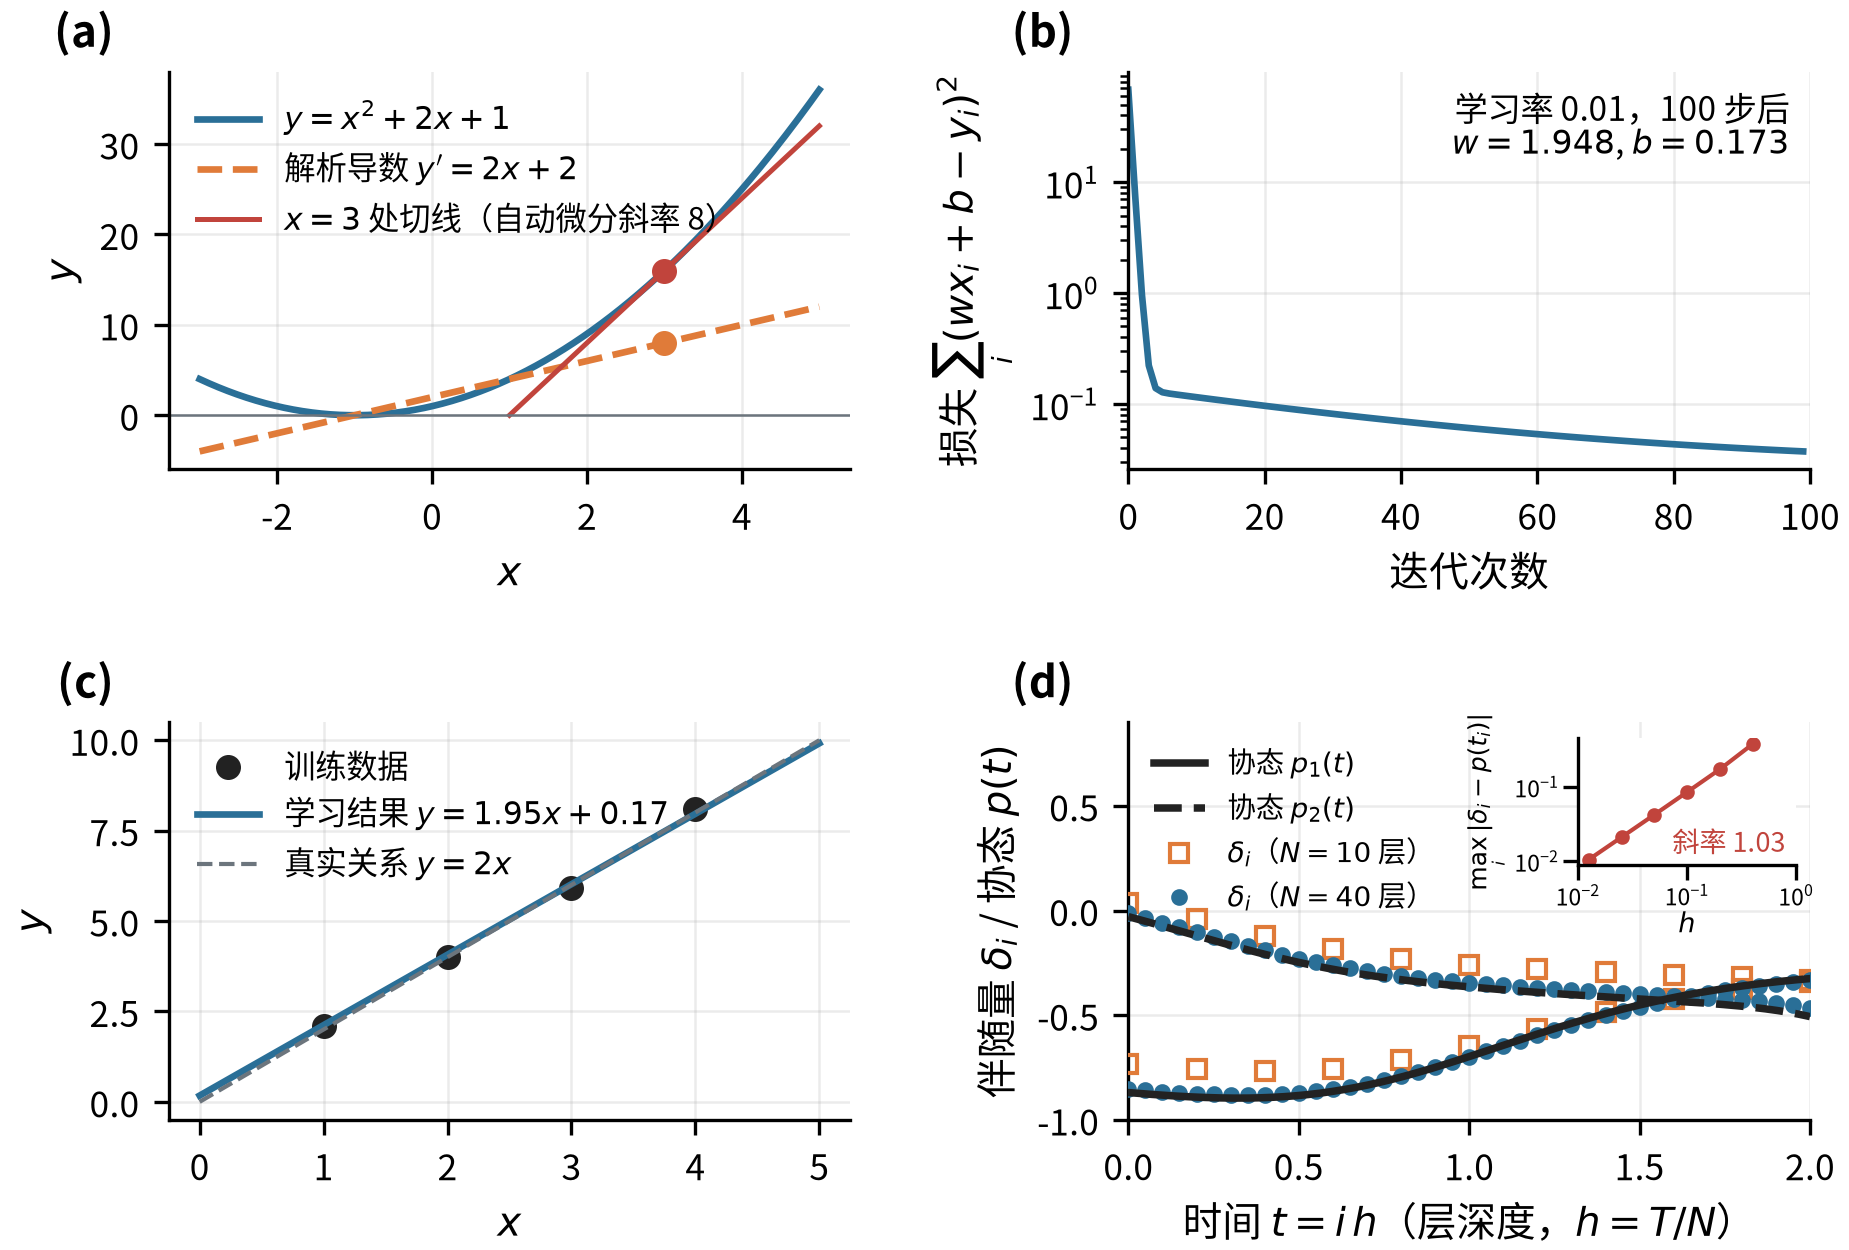
\includegraphics[width=0.95\textwidth]{figs_chap08/chap08_fig1.png}
\caption{最省力移动问题的解析解可视化。左图：最优轨迹$x^*(t) = (t/T)^2(3 - 2t/T)$（位置）和速度曲线——先加速后减速，在中点速度最大；中图：最优控制$u^*(t) = 6/T^2(1 - 2t/T)$——前半段加速（$u > 0$），后半段减速（$u < 0$）；右图：能量消耗随时间长度 $T$ 的关系——时间越长，所需控制能量越小，符合"慢工出细活"的直觉。}
\label{fig:chap08_minimum_effort}
\end{figure}

% ------------------------------------------------------------------------------------
\section{离散时间的视角}

实际计算机控制时，我们不能处理连续时间，必须离散化。这反而让问题变得更清晰！

\subsection{离散化}

把时间 $[0, T]$ 分成 $N$ 段，每段长度 $\Delta t = T/N$。

时刻：$t_k = k \cdot \Delta t$，$k = 0, 1, \ldots, N$

\textbf{离散状态和控制}：
\begin{itemize}
    \item $x_k \approx x(t_k)$：第 $k$ 时刻的状态
    \item $u_k \approx u(t_k)$：第 $k$ 时刻的控制
\end{itemize}

\textbf{离散动力学}（欧拉法）：
\[
x_{k+1} = x_k + \Delta t \cdot f(x_k, u_k)
\]

\textbf{离散代价}：
\[
J = \sum_{k=0}^{N-1} L(x_k, u_k) \cdot \Delta t
\]

\subsection{变成有限维优化问题}

\begin{keyformula}[title=离散轨迹优化]
\begin{equation}
\min_{x_0, u_0, x_1, u_1, \ldots, x_N, u_{N-1}} \sum_{k=0}^{N-1} L(x_k, u_k)
\end{equation}
\begin{align}
\text{s.t.} \quad & x_{k+1} = x_k + \Delta t \cdot f(x_k, u_k), \quad k = 0, \ldots, N-1 \\
& x_0 = x_{init} \\
& x_N = x_{target}
\end{align}
\end{keyformula}

这是一个\textbf{有限维的等式约束优化问题}！可以直接用拉格朗日乘子法。

\subsection{例子：一阶系统，$N = 2$}

考虑一阶系统 $\dot{x} = u$，从 $x(0) = 0$ 到 $x(T) = 1$。

离散化（$N=2$，$\Delta t = T/2$）：
\begin{align}
x_1 &= x_0 + \Delta t \cdot u_0 = \frac{T}{2} u_0 \\
x_2 &= x_1 + \Delta t \cdot u_1 = x_1 + \frac{T}{2} u_1
\end{align}

边界条件：$x_0 = 0$，$x_2 = 1$。

从第一个方程：$x_1 = \frac{T}{2} u_0$

代入第二个方程：$1 = \frac{T}{2} u_0 + \frac{T}{2} u_1$，即 $u_0 + u_1 = \frac{2}{T}$

\textbf{优化问题}：
\[
\min_{u_0, u_1} \frac{1}{2}u_0^2 + \frac{1}{2}u_1^2 \quad \text{s.t.} \quad u_0 + u_1 = \frac{2}{T}
\]

\textbf{用拉格朗日乘子法}：
\[
\mathcal{L} = \frac{1}{2}u_0^2 + \frac{1}{2}u_1^2 + \lambda\left(u_0 + u_1 - \frac{2}{T}\right)
\]

一阶条件：
\begin{align}
\frac{\partial \mathcal{L}}{\partial u_0} &= u_0 + \lambda = 0 \quad \Rightarrow \quad u_0 = -\lambda \\
\frac{\partial \mathcal{L}}{\partial u_1} &= u_1 + \lambda = 0 \quad \Rightarrow \quad u_1 = -\lambda \\
\frac{\partial \mathcal{L}}{\partial \lambda} &= u_0 + u_1 - \frac{2}{T} = 0
\end{align}

从前两个方程：$u_0 = u_1$

代入第三个方程：$2u_0 = \frac{2}{T}$，所以 $u_0 = u_1 = \frac{1}{T}$

\textbf{最优解}：匀速运动！$u_0 = u_1 = \frac{1}{T}$

这与连续时间的解一致（对于一阶系统，最省力的方法就是匀速）。这种"先离散化、再当成普通约束优化来解"的做法叫\textbf{直接法}。
\tryit{把 $N$ 改成 4、8、16，用 \texttt{scipy.optimize.minimize} 加等式约束求解，看 $u_k$ 是否始终等于 $1/T$。再把系统换回二阶的 $\ddot{x} = u$（状态取 $(x, v)$），看数值解如何逼近前面的解析解 $u^*(t) = \frac{6}{T^2}(1 - \frac{2t}{T})$。这就是"直接法"。}

% ------------------------------------------------------------------------------------
\section{伴随方程：反向传播的原型}

这一节我们来仔细推导离散时间的伴随方程，你会发现它和神经网络的反向传播\textbf{完全一样}！

\subsection{离散轨迹优化问题}

先把问题写清楚。我们要解决：

\begin{equation}
\min_{u_0, u_1, \ldots, u_{N-1}} J = \sum_{k=0}^{N-1} L_k(x_k, u_k) + \phi(x_N)
\end{equation}

约束是离散动力学：
\begin{equation}
x_{k+1} = f(x_k, u_k), \quad k = 0, 1, \ldots, N-1
\end{equation}

初始条件 $x_0$ 给定。

\textbf{决策变量}：控制序列 $u_0, u_1, \ldots, u_{N-1}$

\textbf{注意}：状态 $x_1, x_2, \ldots, x_N$ 不是独立的决策变量！一旦给定 $u_0, \ldots, u_{N-1}$，状态就由动力学唯一确定了。

\subsection{用拉格朗日乘子处理动力学约束}

虽然状态由控制决定，但直接计算 $\frac{\partial J}{\partial u_k}$ 很麻烦（因为 $u_k$ 通过动力学影响后面所有的状态）。

聪明的做法：把状态也当作独立变量，用拉格朗日乘子处理动力学约束。

\textbf{构造拉格朗日函数}：

对每个动力学约束 $f(x_k, u_k) - x_{k+1} = 0$（与连续部分的 $f - \dot{x}$ 同一写法），引入乘子 $\lambda_{k+1}$：

\begin{equation}
\mathcal{L} = \underbrace{\sum_{k=0}^{N-1} L_k(x_k, u_k) + \phi(x_N)}_{\text{原目标函数}} + \underbrace{\sum_{k=0}^{N-1} \lambda_{k+1}^\top \left[ f(x_k, u_k) - x_{k+1} \right]}_{\text{约束项（应该=0）}}
\end{equation}

展开写得更清楚：
\begin{align}
\mathcal{L} &= L_0(x_0, u_0) + \lambda_1^\top [f(x_0, u_0) - x_1] \\
&+ L_1(x_1, u_1) + \lambda_2^\top [f(x_1, u_1) - x_2] \\
&+ L_2(x_2, u_2) + \lambda_3^\top [f(x_2, u_2) - x_3] \\
&+ \cdots \\
&+ L_{N-1}(x_{N-1}, u_{N-1}) + \lambda_N^\top [f(x_{N-1}, u_{N-1}) - x_N] \\
&+ \phi(x_N)
\end{align}

\subsection{对各变量求偏导}

现在对 $\mathcal{L}$ 分别对 $x_k$、$u_k$、$\lambda_k$ 求偏导，令其为零。

\paragraph{对 $\lambda_{k+1}$ 求导}（恢复动力学约束）

\[
\frac{\partial \mathcal{L}}{\partial \lambda_{k+1}} = f(x_k, u_k) - x_{k+1} = 0
\]

这就是原来的动力学方程！没有新信息。

\paragraph{对 $u_k$ 求导}（最优性条件）

$u_k$ 只出现在 $L_k(x_k, u_k)$ 和 $f(x_k, u_k)$ 中：

\[
\frac{\partial \mathcal{L}}{\partial u_k} = \frac{\partial L_k}{\partial u_k} + \lambda_{k+1}^\top \frac{\partial f}{\partial u_k} = 0
\]

像连续部分那样定义离散哈密顿量 $H_k = L_k(x_k, u_k) + \lambda_{k+1}^\top f(x_k, u_k)$，这个条件就是：
\begin{equation}
\boxed{\frac{\partial H_k}{\partial u_k} = \frac{\partial L_k}{\partial u_k} + \lambda_{k+1}^\top \frac{\partial f}{\partial u_k} = 0}
\end{equation}

这告诉我们：最优控制时，代价对 $u_k$ 的"直接"敏感度，与"经由下一步状态传回来"的敏感度（乘子 × 动力学对 $u_k$ 的敏感度）恰好抵消。

\paragraph{对 $x_k$（$k = 1, \ldots, N-1$）求导}（伴随方程）

这是最关键的一步！让我们仔细看 $x_k$ 出现在哪里：

\begin{itemize}
    \item $L_k(x_k, u_k)$ 中：贡献 $\frac{\partial L_k}{\partial x_k}$
    \item $\lambda_{k+1}^\top [f(x_k, u_k) - x_{k+1}]$ 中的 $f(x_k, u_k)$：贡献 $\lambda_{k+1}^\top \frac{\partial f}{\partial x_k}$
    \item $\lambda_k^\top [f(x_{k-1}, u_{k-1}) - x_k]$ 中的 $-x_k$：贡献 $-\lambda_k^\top$
\end{itemize}

令偏导为零：
\[
\frac{\partial \mathcal{L}}{\partial x_k} = \frac{\partial L_k}{\partial x_k} - \lambda_k^\top + \lambda_{k+1}^\top \frac{\partial f}{\partial x_k} = 0
\]

整理得到\textbf{伴随方程}：
\begin{equation}
\boxed{\lambda_k = \left(\frac{\partial f}{\partial x_k}\right)^\top \lambda_{k+1} + \frac{\partial L_k}{\partial x_k}^\top = \frac{\partial H_k}{\partial x_k}^\top}
\end{equation}

\paragraph{对 $x_N$ 求导}（终端条件）

$x_N$ 出现在 $\phi(x_N)$ 和 $-\lambda_N^\top x_N$ 中：
\[
\frac{\partial \mathcal{L}}{\partial x_N} = \frac{\partial \phi}{\partial x_N} - \lambda_N^\top = 0
\]

得到\textbf{终端条件}：
\begin{equation}
\boxed{\lambda_N = \frac{\partial \phi}{\partial x_N}^\top}
\end{equation}
\think{$\lambda_N = \partial \phi/\partial x_N$ 说的是"终点状态挪一点，终端代价变多少"——正是影子价格。它和第1章的 $\lambda = -df^*/d\epsilon$ 差一个负号，矛盾吗？（提示：把最后一条约束放松成 $f(x_{N-1}, u_{N-1}) - x_N = \epsilon$，意味着 $x_N$ 减少 $\epsilon$，于是 $dJ^*/d\epsilon = -\partial\phi/\partial x_N = -\lambda_N$，第1章的规则原封不动。）}

\subsection{具体例子：手算伴随方程}

让我们用一个超级简单的例子来验证这些公式。

\textbf{问题}：一维系统，$N = 2$ 步

\begin{itemize}
    \item 动力学：$x_{k+1} = x_k + u_k$（离散积分器）
    \item 代价：$J = u_0^2 + u_1^2 + 10 x_2^2$（最小化控制能量，同时让终点尽量接近零）
    \item 初始条件：$x_0 = 1$
\end{itemize}


\textbf{第一步：前向传播}

\begin{align}
x_1 &= x_0 + u_0 = 1 + u_0 \\
x_2 &= x_1 + u_1 = 1 + u_0 + u_1
\end{align}

\textbf{第二步：计算各偏导数}

动力学 $f(x, u) = x + u$：
\[
\frac{\partial f}{\partial x} = 1, \quad \frac{\partial f}{\partial u} = 1
\]

代价 $L_k = u_k^2$：
\[
\frac{\partial L_k}{\partial x} = 0, \quad \frac{\partial L_k}{\partial u} = 2u_k
\]

终端代价 $\phi = 10 x_2^2$：
\[
\frac{\partial \phi}{\partial x_2} = 20 x_2
\]

\textbf{第三步：后向传播}（计算伴随变量）

终端条件：
\[
\lambda_2 = \frac{\partial \phi}{\partial x_2} = 20 x_2 = 20(1 + u_0 + u_1)
\]

伴随方程（$k = 1$）：
\[
\lambda_1 = \frac{\partial f}{\partial x}^\top \lambda_2 + \frac{\partial L_1}{\partial x}^\top = 1 \cdot \lambda_2 + 0 = \lambda_2 = 20(1 + u_0 + u_1)
\]

\textbf{第四步：最优性条件}

对 $u_1$：
\[
\frac{\partial L_1}{\partial u_1} + \lambda_2 \cdot \frac{\partial f}{\partial u} = 0 \quad \Rightarrow \quad 2u_1 = -\lambda_2 \cdot 1 = -20(1 + u_0 + u_1)
\]

整理：$2u_1 + 20u_1 = -20 - 20u_0$，即 $22u_1 = -20 - 20u_0$

对 $u_0$：
\[
\frac{\partial L_0}{\partial u_0} + \lambda_1 \cdot \frac{\partial f}{\partial u} = 0 \quad \Rightarrow \quad 2u_0 = -\lambda_1 \cdot 1 = -20(1 + u_0 + u_1)
\]

整理：$2u_0 + 20u_0 = -20 - 20u_1$，即 $22u_0 = -20 - 20u_1$

\textbf{第五步：解方程组}

\begin{align}
22u_0 &= -20 - 20u_1 \\
22u_1 &= -20 - 20u_0
\end{align}

两式相减：$22(u_0 - u_1) = -20(u_1 - u_0) = 20(u_0 - u_1)$

所以 $2(u_0 - u_1) = 0$，即 $u_0 = u_1$。

代入第一个方程：$22u_0 = -20 - 20u_0$，得 $42u_0 = -20$，即：
\[
u_0 = u_1 = -\frac{20}{42} = -\frac{10}{21} \approx -0.476
\]

\textbf{验证}：
\begin{align}
x_1 &= 1 + u_0 = 1 - 0.476 = 0.524 \\
x_2 &= x_1 + u_1 = 0.524 - 0.476 = 0.048
\end{align}

终点 $x_2 \approx 0.048$，接近零！

代价：$J = u_0^2 + u_1^2 + 10x_2^2 = 0.227 + 0.227 + 0.023 = 0.477$

\begin{insightbox}
\textbf{我们刚才做了什么？}

\begin{enumerate}
    \item 把优化问题写成拉格朗日函数
    \item 对各变量求导，得到\textbf{伴随方程}
    \item \textbf{前向}计算状态，\textbf{后向}计算伴随变量
    \item 用最优性条件求解最优控制
\end{enumerate}

\end{insightbox}


% ------------------------------------------------------------------------------------
\section{模型预测控制（MPC）}

\subsection{为什么需要 MPC？}

到目前为止，我们假设：
\begin{itemize}
    \item 模型完全准确（动力学 $f$ 精确已知）
    \item 没有外部干扰（没有风、没有摩擦变化）
    \item 可以一次性规划整个轨迹（从头到尾）
\end{itemize}

但现实世界不是这样的！

\begin{figure}[htbp]
\centering
\begin{tikzpicture}[scale=0.9]
    % 理想情况
    \begin{scope}
        \node[font=\bfseries] at (2, 2.5) {理想情况};
        \draw[thick] (0, 0) -- (4, 0);
        \draw[blue, thick, ->] (0.5, 0.3) to[out=30, in=150] (3.5, 0.3);
        \fill[blue] (0.5, 0.3) circle (2pt);
        \fill[red] (3.5, 0.3) circle (2pt);
        \node at (2, -0.5) {\small 规划一次，完美执行};
    \end{scope}
    
    % 现实情况
    \begin{scope}[xshift=6cm]
        \node[font=\bfseries] at (2, 2.5) {现实情况};
        \draw[thick] (0, 0) -- (4, 0);
        \draw[blue, thick, ->] (0.5, 0.3) to[out=30, in=180] (1.5, 0.8);
        \draw[blue, thick, dashed] (1.5, 0.8) to[out=0, in=150] (3.5, 0.3);
        \draw[red, thick, ->] (1.5, 0.8) to[out=-30, in=180] (2.2, 0.2);
        \fill[blue] (0.5, 0.3) circle (2pt);
        \fill[red] (3.5, 0.3) circle (2pt);
        
        % 干扰
        \draw[->, thick, orange] (1.3, 1.5) -- (1.5, 0.9);
        \node[orange] at (1.3, 1.8) {\small 干扰！};
        
        \node at (2, -0.5) {\small 计划被打乱};
    \end{scope}
\end{tikzpicture}
\caption{理想 vs 现实：干扰会打乱预先规划好的轨迹}
\end{figure}

\textbf{具体例子}：

\begin{itemize}
    \item \textbf{模型误差}：你以为摩擦系数是 0.5，实际是 0.3（路面结冰了）
    \item \textbf{外部干扰}：无人机在飞行中突然遇到侧风
    \item \textbf{环境变化}：自动驾驶车前方突然出现行人
\end{itemize}

如果我们在起点规划好整条轨迹然后"闭着眼执行"，一点小扰动就会让系统偏离目标！

\textbf{MPC 的哲学}：\textbf{计划赶不上变化，所以我们边走边规划}！
\think{MPC 每一步都重新解优化问题，那上一步算出的乘子 $\lambda$ 还有用吗？提示：$\lambda$ 是"未来代价对当前状态的敏感度"，而当前状态刚刚被测量更新了。第10章的值函数会给出更系统的答案：它就是"把 $\lambda$ 对所有可能的当前状态预先算好"。}

\subsection{MPC 的核心思想}

\begin{keyformula}[title=MPC 框架]
在\textbf{每个}时刻 $t$：
\begin{enumerate}
    \item \textbf{测量}：获取当前真实状态 $x_t$（通过传感器）
    \item \textbf{规划}：以 $x_t$ 为起点，求解未来 $N$ 步的轨迹优化问题
    \item \textbf{执行}：只执行优化结果的\textbf{第一步}控制 $u_t^*$
    \item \textbf{重复}：下一时刻回到第1步，用新测量的状态重新规划
\end{enumerate}
\end{keyformula}

\begin{figure}[htbp]
\centering
\begin{tikzpicture}[scale=1.0]

    % 时间轴
    \draw[->] (0,0) -- (17,0) node[right] {时间};

    % --------------------------
    % t=0 时刻
    % --------------------------
    \begin{scope}[xshift=0cm]
        \node[above] at (1,2.2) {\small $t=0$};
        \draw[thick] (1,0.1) -- (1,-0.1);

        % 预测轨迹
        \draw[blue, thick] (1,1.4) -- (2,1.6) -- (3,1.5) -- (4,1.3) -- (5,1.1);
        \foreach \x in {1,2,3,4,5} {
            \fill[blue] (\x, {1.4 + 0.2*sin((\x-1)*40)}) circle (2pt);
        }

        \node[blue, above] at (3,1.8) {\small 规划 $N=4$ 步};

        % 执行一步
        \draw[red, ultra thick] (1,0) -- (2,0);
        \draw[red, ultra thick, ->] (1,1.4) -- (2,1.6);
        \node[red, below] at (1.5,-0.3) {\small 执行};
    \end{scope}

    % --------------------------
    % t=1 时刻
    % --------------------------
    \begin{scope}[xshift=5cm]
        \node[above] at (1,2.2) {\small $t=1$};
        \draw[thick] (1,0.1) -- (1,-0.1);

        % 新真实位置
        \fill[orange] (1,1.5) circle (3pt);
        \node[orange,right] at (1.1,1.5) {\small 实际};

        % 新轨迹
        \draw[green!60!black, thick] (1,1.5) -- (2,1.55) -- (3,1.35) -- (4,1.15) -- (5,0.95);
        \node[green!60!black, above] at (3,1.9) {\small 重新规划};

        % 执行
        \draw[red, ultra thick] (1,0) -- (2,0);
    \end{scope}

    % --------------------------
    % t=2 时刻
    % --------------------------
    \begin{scope}[xshift=10cm]
        \node[above] at (1,2.2) {\small $t=2$};
        \draw[thick] (1,0.1) -- (1,-0.1);

        % 实际位置
        \fill[purple] (1,1.4) circle (3pt);

        % 预测轨迹
        \draw[purple, thick, dashed] (1,1.4) -- (2,1.25) -- (3,1.05) -- (4,0.85) -- (5,0.7);

        % 执行
        \draw[red, ultra thick] (1,0) -- (2,0);
    \end{scope}

    % --------------------------
    % 说明框
    % --------------------------
    \node[draw, align=left, fill=yellow!10] at (14,2.0) {
        \small 关键思想：滚动优化\\
        \small 1. 测量真实状态\\
        \small 2. 重新规划未来轨迹\\
        \small 3. 每次只执行一步
    };

\end{tikzpicture}

\caption{MPC 的滚动时域：不断测量、规划、执行}
\end{figure}

\subsection{为什么只执行一步就重新规划？}

这是 MPC 最反直觉的地方：明明规划了 $N$ 步，为什么只用第一步？

\textbf{原因1：近处看得准，远处看不准}

\begin{figure}[htbp]
\centering
\begin{tikzpicture}[scale=0.8]
    \draw[->] (0, 0) -- (8, 0) node[right] {时间};
    \draw[->] (0, 0) -- (0, 3) node[above] {预测误差};
    
    % 误差增长曲线
    \draw[thick, red, domain=0:7, samples=50] plot (\x, {0.1*\x*\x});
    
    % 标注
    \draw[dashed] (1, 0) -- (1, 0.1);
    \draw[dashed] (4, 0) -- (4, 1.6);
    \draw[dashed] (7, 0) -- (7, 4.9);
    
    \node[below] at (1, 0) {\small 第1步};
    \node[below] at (4, 0) {\small 第4步};
    \node[below] at (7, 0) {\small 第7步};
    
    \node[red] at (5, 3) {误差累积！};
\end{tikzpicture}
\caption{预测误差随时间累积：第一步最可靠}
\end{figure}

模型不完美，预测误差会\textbf{累积}。第一步的预测最准，越往后越不可信。

\textbf{原因2：信息会更新}

执行完第一步后，我们\textbf{测量到新的状态}。这是新的信息！用新信息重新规划，比用旧信息盲目执行更明智。

\textbf{原因3：自动纠错}

即使第一步执行得不完美，下一次规划会基于\textbf{实际到达的位置}，自动修正偏差。

\begin{physicalmeaning}
MPC 的生活比喻：

\textbf{开车导航}：
\begin{itemize}
    \item 开环控制：在出发前规划好路线，然后闭着眼开
    \item MPC：每隔几秒重新看一眼导航，根据当前位置调整路线
\end{itemize}

\textbf{下棋}：
\begin{itemize}
    \item 开环控制：一开始就想好后面50步怎么走
    \item MPC：每走一步，看对手怎么应对，再决定下一步
\end{itemize}

MPC 用\textbf{计算量}换取\textbf{鲁棒性}——每一步都重新算，但能应对意外。
\end{physicalmeaning}

\subsection{MPC 的数学形式}

在时刻 $t$，我们求解以下优化问题：

\begin{equation}
\min_{u_t, u_{t+1}, \ldots, u_{t+N-1}} \sum_{k=0}^{N-1} L(x_{t+k}, u_{t+k}) + \phi(x_{t+N})
\end{equation}

约束：
\begin{align}
x_{t+k+1} &= f(x_{t+k}, u_{t+k}), \quad k = 0, \ldots, N-1 \quad \text{（动力学）}\\
x_t &= x_{measured} \quad \text{（\textbf{关键}：用测量值作为初始条件！）}\\
u_{min} &\leq u_{t+k} \leq u_{max} \quad \text{（控制约束，如电机功率有限）}
\end{align}

\textbf{符号说明}：
\begin{itemize}
    \item $N$：预测时域（往前看多少步）
    \item $\phi(x_{t+N})$：终端代价（鼓励最终状态接近目标）
    \item $x_{measured}$：传感器测量的当前状态——\textbf{这就是 MPC 反馈的来源}！
\end{itemize}

% ------------------------------------------------------------------------------------
\section{完整例题：小车刹车问题}

让我们完整地手算一个 MPC 例子。

\subsection{问题设置}

一辆小车在一维轨道上，我们要让它停到原点 $p = 0$。

\textbf{状态}：$x = \begin{pmatrix} p \\ v \end{pmatrix}$，其中 $p$ = 位置，$v$ = 速度

\textbf{控制}：$u$ = 加速度（正 = 加速，负 = 刹车）

\textbf{离散动力学}（$\Delta t = 1$ 秒，简化计算）：
\begin{align}
p_{k+1} &= p_k + v_k \\
v_{k+1} &= v_k + u_k
\end{align}

写成矩阵形式：
\[
x_{k+1} = \underbrace{\begin{pmatrix} 1 & 1 \\ 0 & 1 \end{pmatrix}}_{A} x_k + \underbrace{\begin{pmatrix} 0 \\ 1 \end{pmatrix}}_{B} u_k
\]

\textbf{代价函数}（希望位置和速度都接近零，同时不要用太大的控制）：
\[
J = \sum_{k=0}^{N-1} (p_k^2 + v_k^2 + 0.1 u_k^2) + 10(p_N^2 + v_N^2)
\]

\textbf{当前状态}：$x_0 = \begin{pmatrix} 3 \\ 2 \end{pmatrix}$（位置 3m，速度 2m/s，正在远离原点！）

\textbf{预测时域}：$N = 2$（只看两步，便于手算）

\subsection{第一步：写出状态递推}

给定 $x_0$ 和控制 $u_0, u_1$，计算 $x_1, x_2$：

\[
x_1 = A x_0 + B u_0 = \begin{pmatrix} 1 & 1 \\ 0 & 1 \end{pmatrix} \begin{pmatrix} 3 \\ 2 \end{pmatrix} + \begin{pmatrix} 0 \\ 1 \end{pmatrix} u_0 = \begin{pmatrix} 5 \\ 2 + u_0 \end{pmatrix}
\]

\[
x_2 = A x_1 + B u_1 = \begin{pmatrix} 1 & 1 \\ 0 & 1 \end{pmatrix} \begin{pmatrix} 5 \\ 2 + u_0 \end{pmatrix} + \begin{pmatrix} 0 \\ 1 \end{pmatrix} u_1 = \begin{pmatrix} 7 + u_0 \\ 2 + u_0 + u_1 \end{pmatrix}
\]

所以：
\begin{align}
p_1 &= 5, \quad v_1 = 2 + u_0 \\
p_2 &= 7 + u_0, \quad v_2 = 2 + u_0 + u_1
\end{align}

\subsection{第二步：写出代价函数}

\begin{align}
J &= (p_0^2 + v_0^2 + 0.1 u_0^2) + (p_1^2 + v_1^2 + 0.1 u_1^2) + 10(p_2^2 + v_2^2) \\
&= (9 + 4 + 0.1 u_0^2) + (25 + (2+u_0)^2 + 0.1 u_1^2) + 10((7+u_0)^2 + (2+u_0+u_1)^2)
\end{align}

展开（只保留与 $u_0, u_1$ 有关的项，因为常数不影响最优化）：

\begin{align}
J &= 0.1 u_0^2 + (2+u_0)^2 + 0.1 u_1^2 + 10(7+u_0)^2 + 10(2+u_0+u_1)^2 + \text{const} \\
&= 0.1 u_0^2 + (4 + 4u_0 + u_0^2) + 0.1 u_1^2 + 10(49 + 14u_0 + u_0^2) \\
&\quad + 10(4 + 4u_0 + 4u_1 + u_0^2 + 2u_0 u_1 + u_1^2) + \text{const}
\end{align}

整理 $u_0, u_1$ 的系数：
\begin{align}
J &= (0.1 + 1 + 10 + 10) u_0^2 + (0.1 + 10) u_1^2 + 20 u_0 u_1 \\
&\quad + (4 + 140 + 40) u_0 + (40) u_1 + \text{const} \\
&= 21.1 u_0^2 + 10.1 u_1^2 + 20 u_0 u_1 + 184 u_0 + 40 u_1 + \text{const}
\end{align}

\subsection{第三步：求最优控制}

对 $u_0, u_1$ 求偏导，令其为零：
\begin{align}
\frac{\partial J}{\partial u_0} &= 42.2 u_0 + 20 u_1 + 184 = 0 \\
\frac{\partial J}{\partial u_1} &= 20.2 u_1 + 20 u_0 + 40 = 0
\end{align}

从第二个方程：$u_1 = \frac{-40 - 20 u_0}{20.2} = \frac{-40 - 20 u_0}{20.2}$

代入第一个方程：
\[
42.2 u_0 + 20 \cdot \frac{-40 - 20 u_0}{20.2} + 184 = 0
\]

\[
42.2 u_0 - \frac{800 + 400 u_0}{20.2} + 184 = 0
\]

乘以 20.2：
\[
852.44 u_0 - 800 - 400 u_0 + 3716.8 = 0
\]

\[
452.44 u_0 = -2916.8
\]

\[
u_0^* \approx -6.45
\]

代回求 $u_1$：
\[
u_1^* = \frac{-40 - 20 \times (-6.45)}{20.2} = \frac{-40 + 129.0}{20.2} \approx 4.40
\]

\subsection{第四步：MPC 只执行第一步}

最优控制序列是 $(u_0^*, u_1^*) \approx (-6.45, 4.40)$。

\textbf{但 MPC 只执行 $u_0^* = -6.45$}（猛踩刹车！）

执行后，真实状态变为：
\[
x_1 = \begin{pmatrix} 5 \\ 2 + (-6.45) \end{pmatrix} = \begin{pmatrix} 5 \\ -4.45 \end{pmatrix}
\]

位置到了 5m，但速度变成了 $-4.45$ m/s（开始往回走了！）

\subsection{第五步：重新规划}

下一时刻，用新的初始状态 $x_0^{new} = \begin{pmatrix} 5 \\ -4.45 \end{pmatrix}$ 重新求解优化问题。

（计算过程类似，这里省略）

新的最优控制会考虑到"现在正在往回走"这个事实，给出合适的控制。

\begin{insightbox}
\textbf{MPC 的精髓}：

我们规划了 $u_0^* \approx -6.45, u_1^* \approx 4.40$，但\textbf{只执行 $u_0^*$}。

为什么不执行 $u_1^*$？因为：
\begin{itemize}
    \item 执行 $u_0$ 后，真实状态可能不是预测的 $x_1$（有误差）
    \item 用\textbf{真实测量的状态}重新规划，比用\textbf{预测的状态}盲目执行更可靠
\end{itemize}

这就是 MPC 的反馈特性：\textbf{每一步都用最新信息做最优决策}。
\end{insightbox}

\subsection{MPC 的反馈修正能力}

假设执行 $u_0 = -6.45$ 后，因为路面打滑，实际状态不是 $\begin{pmatrix} 5 \\ -4.45 \end{pmatrix}$，而是 $\begin{pmatrix} 5.5 \\ -3.5 \end{pmatrix}$。

\textbf{开环控制}：继续执行预先计划的 $u_1 = 4.40$，不管实际状态如何。结果可能偏离目标。

\textbf{MPC}：用实际测量的 $\begin{pmatrix} 5.5 \\ -3.5 \end{pmatrix}$ 重新规划。新的 $u_1^{new}$ 会自动补偿偏差！

这就是 MPC 强大的原因：\textbf{它把优化问题嵌入到反馈回路中}，自动适应实际情况。

% ------------------------------------------------------------------------------------
% 代码演示结果
\begin{figure}[htbp]
\centering
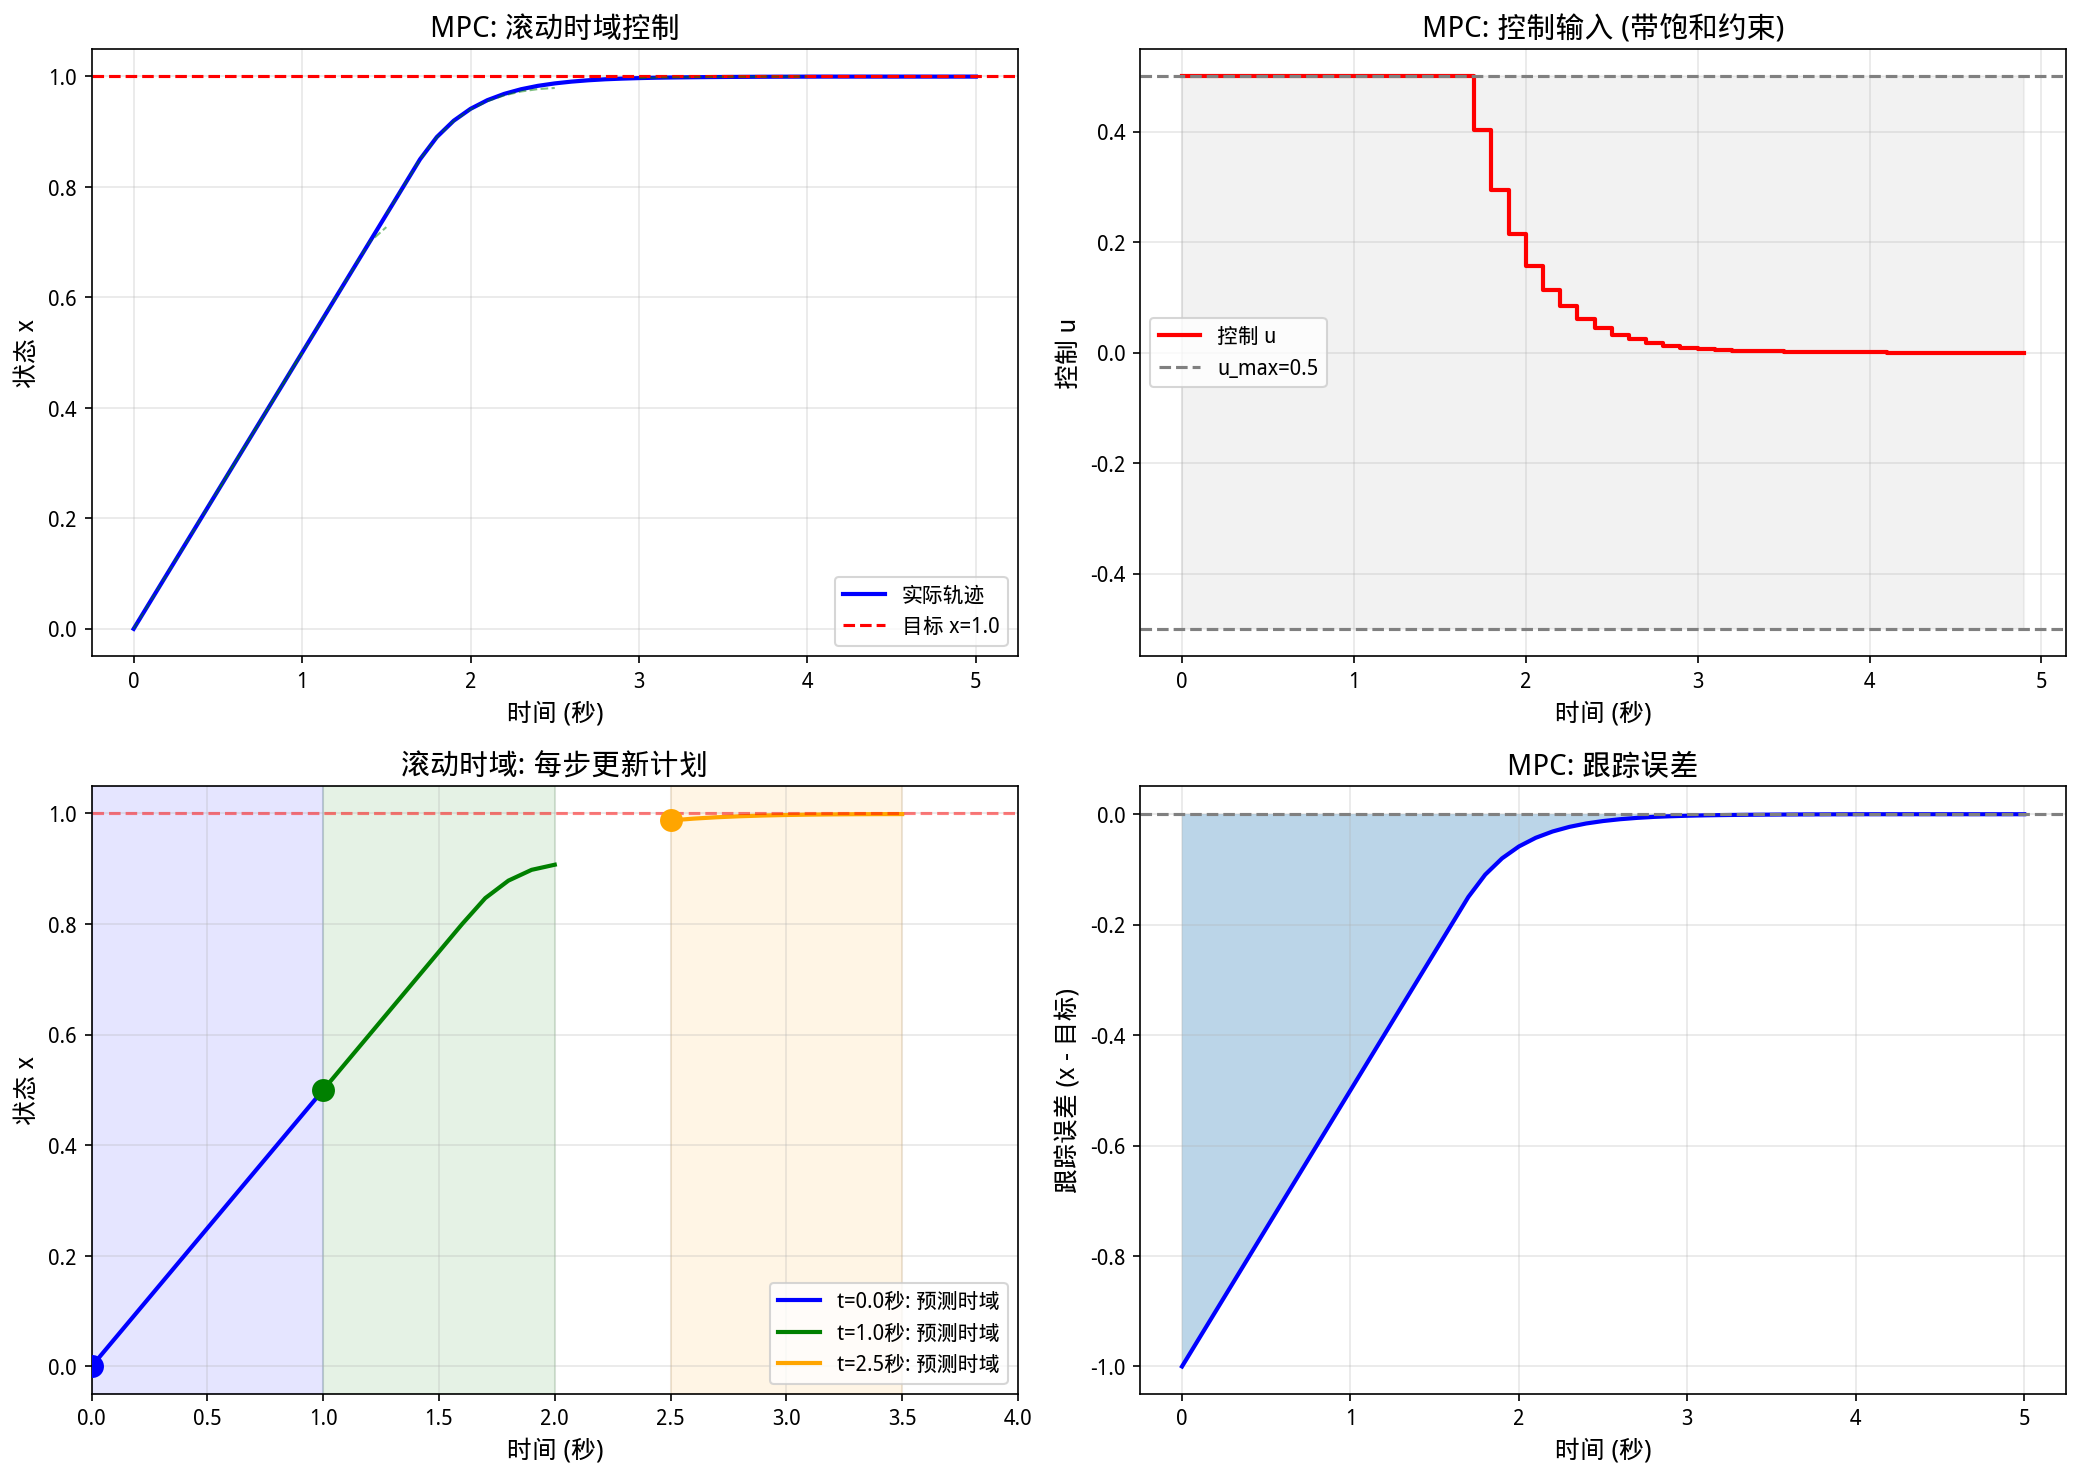
\includegraphics[width=0.98\textwidth]{figs_chap08/chap08_fig2.png}
\caption{MPC（模型预测控制）滚动时域演示。左上：实际轨迹与多条预测轨迹——每个时刻重新规划，但只执行第一步；右上：控制输入（饱和在$\pm 0.5$）；左下：滚动时域示意——不同时刻的规划窗口；右下：跟踪误差随时间减小。MPC的核心思想：规划多步但只执行一步，用反馈不断修正。}
\label{fig:chap08_mpc}
\end{figure}

% ------------------------------------------------------------------------------------
\section{本章小结}

\begin{enumerate}
    \item \textbf{轨迹优化}是带微分方程约束的变分问题
    
    \item \textbf{拉格朗日乘子} $\lambda(t)$ 处理动力学约束，物理意义是"未来对现在的影响"
    
    \item \textbf{哈密顿函数} $H = L + \lambda^\top f$ 是拉格朗日函数的连续时间版本
    
    \item \textbf{伴随方程}向后积分，与神经网络的\textbf{反向传播}数学结构相同
    
    \item \textbf{MPC} 是"边走边规划"的策略：规划多步，执行一步，用反馈修正
\end{enumerate}

\begin{unification}[title=统一视角：约束优化无处不在]
\begin{center}
\begin{tabular}{lll}
\toprule
\textbf{问题} & \textbf{约束} & \textbf{乘子的意义} \\
\midrule
静态优化 & $g(x) = 0$ & 约束的"价格" \\
力学系统 & 运动学约束 & 约束力 \\
轨迹优化 & $\dot{x} = f(x, u)$ & 未来代价的敏感度 \\
神经网络 & $z_{k+1} = f(z_k, W_k)$ & 损失对中间层的梯度 \\
\bottomrule
\end{tabular}
\end{center}

从静态到动态，从有限维到无限维，拉格朗日乘子法的思想贯穿始终！
\end{unification}

\begin{physicalmeaning}
\textbf{$\lambda$ 在本章的意义}：$\lambda(t)$ 是动力学约束在时刻 $t$ 的影子价格——"如果此刻有人把状态 $x(t)$ 推开 $\epsilon$，从现在到终点的最小代价会变化 $\lambda(t)^\top \epsilon$"。它有三张面孔：
\begin{itemize}
    \item 往前看第3、4章：把 $L$ 换成拉格朗日量，$\lambda = \partial L/\partial \dot{q}$ 就是广义动量 $p$，伴随方程 $\dot{\lambda} = -\partial H/\partial x$ 就是哈密顿方程 $\dot{p} = -\partial H/\partial q$。
    \item 往后看第9章：把时间步 $k$ 换成网络层 $i$，$\lambda_k$ 就是"误差信号"，伴随方程就是反向传播。
    \item 再往后看第10章：把终点推到无穷远、把代价换成奖励，$\lambda$ 就是值函数的梯度 $\nabla_s V(s)$，伴随方程就变成贝尔曼方程。
\end{itemize}
\end{physicalmeaning}

% ------------------------------------------------------------------------------------
\section{习题}

\paragraph{计算题}
\begin{enumerate}
    \item 对于一维系统 $\dot{x} = u$，最小化 $\int_0^1 u^2 dt$，边界条件 $x(0) = 0$，$x(1) = 1$。
    \begin{enumerate}
        \item 写出哈密顿函数
        \item 写出状态方程、伴随方程、最优性条件
        \item 求解最优控制 $u^*(t)$
        \item 验证 $x^*(t) = t$（匀速运动）
    \end{enumerate}
    
    \item 考虑带终端代价的问题：$\min \int_0^1 \frac{1}{2}u^2 dt + (x(1) - 1)^2$，动力学 $\dot{x} = u$，$x(0) = 0$。
    \begin{enumerate}
        \item 这个问题的终端条件是自由的（不要求 $x(1) = 1$）。推导终端条件 $\lambda(1) = ?$
        \item 求解最优轨迹
    \end{enumerate}
    
    \item （离散化）将问题1离散化为 $N = 4$ 步，用拉格朗日乘子法求解离散最优控制 $u_0^*, u_1^*, u_2^*, u_3^*$。验证与连续解的一致性。
\end{enumerate}

\paragraph{编程题}
\begin{enumerate}
    \setcounter{enumi}{3}
    \item 用直接法数值求解最省力移动问题：把 $\ddot{x} = u$ 离散成 $N = 50$ 步，状态取 $(x_k, v_k)$，用 \texttt{scipy.optimize.minimize}（SLSQP）在等式约束下最小化 $\sum_k u_k^2 \Delta t$。画出 $u_k$，与解析解 $u^*(t) = \frac{6}{T^2}(1 - \frac{2t}{T})$ 比较；打印求解器返回的乘子，验证它们近似等于 $\lambda(t_k)$。
    
    \item 实现本章"小车刹车"的 MPC 控制器：预测时域 $N = 5$，控制受限 $|u_k| \le 3$，每一步只执行 $u_0^*$；在仿真中加入随机扰动（速度每步加上 $\mathcal{N}(0, 0.3^2)$ 的噪声），比较开环控制与 MPC 的轨迹。
\end{enumerate}

\paragraph{思考题}
\begin{enumerate}
    \setcounter{enumi}{5}
    \item 伴随方程为什么要\textbf{向后}积分？这和"未来影响现在"有什么关系？
    
    \item MPC 每步都要求解一个优化问题，计算量很大。有什么方法可以加速？
    
    \item 如果模型不准确（真实动力学和假设的不同），MPC 还能工作吗？为什么？
    
    \item 比较 MPC 和强化学习：
    \begin{itemize}
        \item MPC 需要知道模型 $f(x, u)$，强化学习不需要
        \item MPC 在线计算，强化学习离线训练
        \item 它们各有什么优缺点？
    \end{itemize}
    \preview{第10章会正面回答这道题：强化学习的值函数 $V(s)$ 就是本章的乘子（对所有状态预先算好的 $\lambda$），贝尔曼方程就是伴随方程的无限时域版本；MPC 与强化学习的差别，是"在线解 $\lambda$"还是"离线学 $V$"。}
\end{enumerate}

\paragraph{拓展题}
\begin{enumerate}
    \setcounter{enumi}{9}
    \item （倒立摆）倒立摆的动力学是非线性的。查阅资料，了解如何用线性化 + MPC 控制倒立摆。
    
    \item （Neural ODE）了解"神经常微分方程"的概念。它如何把神经网络和常微分方程统一起来？
\end{enumerate}

% ====================================================================================
\section*{扩展阅读：约束、投影与"能不能到达"的问题}
\addcontentsline{toc}{section}{扩展阅读：约束、投影与"能不能到达"的问题}
% ====================================================================================

在本章中，我们学习了轨迹优化：给定起点和终点，找最优路径。但有一个更基本的问题我们还没问：

\textbf{这条路径存在吗？从 $A$ 出发，我们能不能到达 $B$？}

这就是\textbf{能控性}（controllability）问题。

让我们从一个生活中的例子开始。

%------------------------------------------------------------------------------
\subsection*{一个停车问题}
%------------------------------------------------------------------------------

假设你要把车停进一个平行车位。

\begin{figure}[htbp]
\centering
\begin{tikzpicture}[scale=0.85]
    % 停车位
    \fill[gray!20] (4, -0.5) rectangle (7, 1.5);
    \draw[thick] (4, -0.5) -- (4, 1.5);
    \draw[thick] (7, -0.5) -- (7, 1.5);
    \node at (5.5, 0.5) {\small 车位};
    
    % 初始位置的车
    \begin{scope}[shift={(1, 2)}, rotate=0]
        \draw[thick, fill=blue!30] (-0.6, -0.3) rectangle (0.6, 0.3);
        \fill (0.4, 0.25) circle (1.5pt);
        \fill (0.4, -0.25) circle (1.5pt);
        \fill (-0.4, 0.25) circle (1.5pt);
        \fill (-0.4, -0.25) circle (1.5pt);
    \end{scope}
    \node[blue] at (1, 2.8) {\small 你的车};
    
    % 目标位置的车（虚线）
    \begin{scope}[shift={(5.5, 0.5)}, rotate=0]
        \draw[thick, dashed, red] (-0.6, -0.3) rectangle (0.6, 0.3);
    \end{scope}
    \node[red] at (5.5, -0.3) {\small 目标};
    
    % 问号
    \node[font=\Large] at (3, 1.5) {?};
\end{tikzpicture}
\caption{平行泊车：怎么把车停进去？}
\end{figure}

你有两个控制：
\begin{itemize}
    \item 油门/刹车：控制前进或后退
    \item 方向盘：控制转向
\end{itemize}

\textbf{关键观察}：车不能横着走！

你没法让车直接"平移"进车位。但是，通过前进、后退、转向的组合，你确实可以把车停进去。

\textbf{问题}：为什么两个控制（油门和方向盘）可以让车在三维空间（位置 $x, y$ 和朝向 $\theta$）中自由移动？

答案和我们熟悉的\textbf{约束优化}有深刻的联系。

%------------------------------------------------------------------------------
\subsection*{从约束优化说起}
%------------------------------------------------------------------------------

让我们回顾一下约束优化的核心思想。

\paragraph{等式约束下的优化}

考虑问题：
\begin{equation}
\min f(x) \quad \text{s.t.} \quad g(x) = 0
\end{equation}

约束 $g(x) = 0$ 把我们限制在一个曲面上。在这个曲面上，我们不能朝任意方向走——只能沿着曲面的\textbf{切方向}走。

\begin{figure}[htbp]
\centering
\begin{tikzpicture}[scale=1.0]
    % 曲面（简化为曲线）
    \draw[thick, blue] plot[smooth, domain=-2:2] (\x, {0.3*\x*\x});
    \node[blue] at (2.5, 1.2) {约束曲面};
    
    % 当前点
    \fill[red] (1, 0.3) circle (3pt);
    \node[red, above right] at (1, 0.3) {$x$};
    
    % 切方向（可行）
    \draw[->, green!60!black, very thick] (1, 0.3) -- (2, 0.9);
    \node[green!60!black, right] at (2, 0.9) {切方向（可行）};
    
    % 法方向（不可行）
    \draw[->, gray, thick, dashed] (1, 0.3) -- (1, 1.3);
    \node[gray, right] at (1, 1.3) {法方向（不可行）};
    
    % 梯度
    \draw[->, orange, thick] (1, 0.3) -- (0.4, 0.9);
    \node[orange, left] at (0.4, 0.9) {$\nabla g$};
\end{tikzpicture}
\caption{约束曲面上，只能沿切方向移动}
\end{figure}

\paragraph{可行方向}

在点 $x$ 处，\textbf{可行方向}是满足以下条件的方向 $v$：
\begin{equation}
\nabla g(x)^\top v = 0
\end{equation}

也就是说，$v$ 必须垂直于约束的梯度 $\nabla g$——这样才能保持在约束曲面上。

所有可行方向构成一个\textbf{子空间}——约束曲面的\textbf{切空间}。

\paragraph{投影的视角}

如果我们想朝某个方向 $d$ 走，但 $d$ 不是可行方向怎么办？

答案是：把 $d$ \textbf{投影}到切空间上！

\begin{equation}
d_{\text{可行}} = d - \frac{\nabla g^\top d}{\|\nabla g\|^2} \nabla g
\end{equation}

这就是\textbf{投影梯度法}的核心思想：先计算梯度，再投影到可行方向上。

%------------------------------------------------------------------------------
\subsection*{控制系统中的"约束"}
%------------------------------------------------------------------------------

现在让我们把这个思想用到控制系统上。

\paragraph{汽车的运动学}

汽车的状态是 $(x, y, \theta)$：位置和朝向。

运动方程：
\begin{align}
\dot{x} &= v \cos\theta \\
\dot{y} &= v \sin\theta \\
\dot{\theta} &= \omega
\end{align}

其中 $v$ 是速度（前进/后退），$\omega$ 是转向角速度。

\paragraph{瞬时可达方向}

在任意状态 $(x, y, \theta)$，通过选择 $v$ 和 $\omega$，状态的变化率 $(\dot{x}, \dot{y}, \dot{\theta})$ 可以是：

\begin{equation}
\begin{pmatrix} \dot{x} \\ \dot{y} \\ \dot{\theta} \end{pmatrix} = 
v \underbrace{\begin{pmatrix} \cos\theta \\ \sin\theta \\ 0 \end{pmatrix}}_{g_1} + 
\omega \underbrace{\begin{pmatrix} 0 \\ 0 \\ 1 \end{pmatrix}}_{g_2}
\end{equation}

这意味着：瞬时可达的方向是 $g_1$ 和 $g_2$ 的\textbf{线性组合}。

\paragraph{问题来了}

$g_1$ 和 $g_2$ 只张成一个\textbf{二维}子空间！

但状态空间是三维的 $(x, y, \theta)$。

\textbf{缺失的方向是什么？}

\begin{itemize}
    \item $g_1 = (\cos\theta, \sin\theta, 0)$：沿车身方向（前进/后退）
    \item $g_2 = (0, 0, 1)$：原地转向
\end{itemize}

缺失的是：$(\sin\theta, -\cos\theta, 0)$——\textbf{垂直于车身的方向}（横向移动）！

\begin{figure}[htbp]
\centering
\begin{tikzpicture}[scale=1.1]
    % 三维坐标系
    \draw[->] (0, 0) -- (4, 0) node[right] {$x$};
    \draw[->] (0, 0) -- (0, 3) node[above] {$y$};
    \draw[->] (0, 0) -- (-1.5, -1) node[below left] {$\theta$};
    
    % 车的位置（在 xy 平面上）
    \begin{scope}[shift={(2, 1.5)}]
        % 车身（朝向约30度）
        \draw[thick, fill=gray!30, rotate=30] (-0.4, -0.2) rectangle (0.4, 0.2);
        
        % g1: 前进方向（在xy平面内）
        \draw[->, blue, very thick, rotate=30] (0, 0) -- (1.2, 0);
        \node[blue, rotate=30] at (1.1, 0.5) {$g_1$};
        \node[blue, font=\small] at (2.2, 1.8) {前进/后退};
        
        % 缺失的方向（垂直于车身，在xy平面内）
        \draw[->, red, very thick, dashed, rotate=30] (0, 0) -- (0, -1);
        \node[red, font=\small] at (1.8, -0.2) {缺失！};
        \node[red, font=\small] at (2.8, -0.5) {（横向移动）};
    \end{scope}
    
    % g2: 转向（沿theta轴）
    \draw[->, green!60!black, very thick] (2, 1.5) -- (1, 0.8);
    \node[green!60!black] at (0.5, 1.3) {$g_2$};
    \node[green!60!black, font=\small] at (0.3, 0.7) {转向};
    
    % 说明g1和g2张成的平面
    \fill[blue!10, opacity=0.5] (2, 1.5) -- (3.5, 2.1) -- (2.5, 1.1) -- (1, 0.8) -- cycle;
    \node[font=\small] at (3.8, 0.5) {$g_1, g_2$ 张成的};
    \node[font=\small] at (3.8, 0.1) {二维子空间};
    
    % 标注状态空间是三维
    \draw[<->, thick, purple] (5, 0) -- (5, 2.5);
    \node[purple, font=\small, align=center] at (5.8, 1.25) {状态空间\\是三维的};
\end{tikzpicture}
\caption{$g_1$（前进）和 $g_2$（转向）只张成二维子空间，缺失了横向移动的方向}
\end{figure}

这就是为什么车不能直接横着走。

%------------------------------------------------------------------------------
\subsection*{关键问题：怎么产生新方向？}
%------------------------------------------------------------------------------

虽然不能\textbf{瞬时}横移，但能不能通过某种\textbf{组合操作}实现横移呢？

\paragraph{一个思想实验}

想象以下操作（每步走很小的距离 $\epsilon$）：

\begin{enumerate}
    \item 前进一点点
    \item 左转一点点
    \item 后退一点点
    \item 右转一点点（回到原来的朝向）
\end{enumerate}

如果每步都是"直线运动"，走完一圈应该回到原点。

但实际上呢？

\begin{figure}[htbp]
\centering
\begin{tikzpicture}[scale=1.8]
    % 起点
    \fill (0, 0) circle (2pt);
    \node[below] at (0, 0) {起点};
    
    % 第一步：前进（车朝右）
    \draw[->, blue, thick] (0, 0) -- (0.8, 0);
    \node[blue, above] at (0.4, 0) {\small 1. 前进};
    
    % 第二步：左转（车现在朝上）+ 由于在新位置，"前进"方向变了
    \draw[->, red, thick] (0.8, 0) -- (0.8, 0.6);
    \node[red, right] at (0.8, 0.3) {\small 2. 转+走};
    
    % 第三步：后退
    \draw[->, blue, thick, dashed] (0.8, 0.6) -- (0.1, 0.6);
    \node[blue, above] at (0.45, 0.6) {\small 3. 后退};
    
    % 第四步：右转回来
    \draw[->, red, thick, dashed] (0.1, 0.6) -- (0.1, 0.15);
    \node[red, left] at (0.1, 0.35) {\small 4. 转回};
    
    % 净位移
    \draw[->, green!60!black, very thick] (0, 0) -- (0.1, 0.15);
    \node[green!60!black, below right] at (0.05, 0.08) {净位移！};
    
    % 说明
    \node[align=left] at (2.5, 0.3) {走了一圈\\没回到原点！};
\end{tikzpicture}
\caption{前进—转向—后退—转回：产生了横向位移}
\end{figure}

\textbf{惊喜}：走完一圈，车不在原来的位置！产生了一个\textbf{横向的净位移}。

这就是平行泊车的秘密：虽然不能直接横移，但通过"绕圈"可以\textbf{间接}实现横移。

\paragraph{数学推导：为什么会有净位移？}

让我们用微分方程来严格计算。设初始状态为 $(x_0, y_0, \theta_0) = (0, 0, 0)$（在原点，朝右）。

\textbf{第1步：前进 $\epsilon$}

控制 $v = 1, \omega = 0$，持续时间 $\epsilon$：
\begin{align}
x_1 &= x_0 + \epsilon \cos\theta_0 = 0 + \epsilon \cdot 1 = \epsilon \\
y_1 &= y_0 + \epsilon \sin\theta_0 = 0 + \epsilon \cdot 0 = 0 \\
\theta_1 &= \theta_0 = 0
\end{align}

状态变为 $(\epsilon, 0, 0)$。

\textbf{第2步：左转 $\epsilon$}

控制 $v = 0, \omega = 1$，持续时间 $\epsilon$：
\begin{align}
x_2 &= x_1 = \epsilon \\
y_2 &= y_1 = 0 \\
\theta_2 &= \theta_1 + \epsilon = \epsilon
\end{align}

状态变为 $(\epsilon, 0, \epsilon)$。注意：车现在朝向改变了！

\textbf{第3步：后退 $\epsilon$}

控制 $v = -1, \omega = 0$，持续时间 $\epsilon$。

\textbf{关键}：现在 $\theta = \epsilon \neq 0$，所以"后退"的方向变了！
\begin{align}
x_3 &= x_2 - \epsilon \cos\theta_2 = \epsilon - \epsilon \cos\epsilon \\
y_3 &= y_2 - \epsilon \sin\theta_2 = 0 - \epsilon \sin\epsilon \\
\theta_3 &= \theta_2 = \epsilon
\end{align}

用泰勒展开（$\epsilon$ 很小）：$\cos\epsilon \approx 1 - \frac{\epsilon^2}{2}$，$\sin\epsilon \approx \epsilon$
\begin{align}
x_3 &\approx \epsilon - \epsilon(1 - \frac{\epsilon^2}{2}) = \frac{\epsilon^3}{2} \\
y_3 &\approx -\epsilon \cdot \epsilon = -\epsilon^2
\end{align}

\textbf{第4步：右转 $\epsilon$}

控制 $v = 0, \omega = -1$，持续时间 $\epsilon$：
\begin{align}
x_4 &= x_3 \approx \frac{\epsilon^3}{2} \\
y_4 &= y_3 \approx -\epsilon^2 \\
\theta_4 &= \theta_3 - \epsilon = 0
\end{align}

\textbf{最终结果}：
\begin{equation}
\boxed{(x_4, y_4, \theta_4) \approx \left(\frac{\epsilon^3}{2}, -\epsilon^2, 0\right)}
\end{equation}

\textbf{分析}：
\begin{itemize}
    \item $\theta$ 回到了 0（朝向恢复）
    \item $x$ 方向有 $O(\epsilon^3)$ 的小位移（可忽略）
    \item $y$ 方向有 $\boxed{-\epsilon^2}$ 的位移——这就是\textbf{横向净位移}！
\end{itemize}

虽然每一步都只能沿 $g_1$ 或 $g_2$ 方向走，但四步组合下来，产生了一个沿"缺失方向"（$-y$ 方向，即 $[g_1, g_2]$ 方向）的净位移，大小正比于 $\epsilon^2$。

%------------------------------------------------------------------------------
\subsection*{数学描述：李括号}
%------------------------------------------------------------------------------

刚才的"绕圈产生新方向"现象，数学上用\textbf{李括号}（Lie bracket）来描述。

\paragraph{定义}

给定两个向量场 $f$ 和 $g$，它们的李括号 $[f, g]$ 定义为：

\begin{equation}
[f, g] = \frac{\partial g}{\partial x} f - \frac{\partial f}{\partial x} g
\end{equation}

这里 $\frac{\partial f}{\partial x}$ 是 $f$ 的雅可比矩阵（就是我们熟悉的多元函数求导）。

\paragraph{几何意义}

$[f, g]$ 正是"沿 $f$ 走一点、沿 $g$ 走一点、沿 $-f$ 走回来、沿 $-g$ 走回来"产生的\textbf{净位移方向}。

更精确地：如果每步走 $\epsilon$，净位移大约是 $\epsilon^2 \cdot [f, g]$。

\paragraph{为什么会有净位移？}

关键在于：向量场 $f$ 和 $g$ 是\textbf{随位置变化}的！

在不同位置，$f$ 指向不同方向。所以"前进"和"后退"不是简单的互相抵消——在不同位置执行，效果不完全相反。

这就像在地球上走路：从北京向东走1000公里，再向北走1000公里，再向西走1000公里，再向南走1000公里——你不会回到北京！因为地球是弯的，"东"和"西"的方向随位置而变。

%------------------------------------------------------------------------------
\subsection*{手算汽车的李括号}
%------------------------------------------------------------------------------

让我们来算一下汽车系统的 $[g_1, g_2]$。

\paragraph{两个向量场}

\begin{equation}
g_1 = \begin{pmatrix} \cos\theta \\ \sin\theta \\ 0 \end{pmatrix}, \quad
g_2 = \begin{pmatrix} 0 \\ 0 \\ 1 \end{pmatrix}
\end{equation}

\paragraph{计算雅可比矩阵}

$g_1$ 对 $(x, y, \theta)$ 的偏导：
\begin{equation}
\frac{\partial g_1}{\partial (x, y, \theta)} = \begin{pmatrix} 
\frac{\partial (\cos\theta)}{\partial x} & \frac{\partial (\cos\theta)}{\partial y} & \frac{\partial (\cos\theta)}{\partial \theta} \\
\frac{\partial (\sin\theta)}{\partial x} & \frac{\partial (\sin\theta)}{\partial y} & \frac{\partial (\sin\theta)}{\partial \theta} \\
0 & 0 & 0
\end{pmatrix} = \begin{pmatrix} 0 & 0 & -\sin\theta \\ 0 & 0 & \cos\theta \\ 0 & 0 & 0 \end{pmatrix}
\end{equation}

$g_2$ 是常向量（不依赖于 $x, y, \theta$），所以：
\begin{equation}
\frac{\partial g_2}{\partial (x, y, \theta)} = \begin{pmatrix} 0 & 0 & 0 \\ 0 & 0 & 0 \\ 0 & 0 & 0 \end{pmatrix}
\end{equation}

\paragraph{计算李括号}

\begin{align}
[g_1, g_2] &= \frac{\partial g_2}{\partial x} g_1 - \frac{\partial g_1}{\partial x} g_2 \\
&= \mathbf{0} - \begin{pmatrix} 0 & 0 & -\sin\theta \\ 0 & 0 & \cos\theta \\ 0 & 0 & 0 \end{pmatrix} \begin{pmatrix} 0 \\ 0 \\ 1 \end{pmatrix} \\
&= -\begin{pmatrix} -\sin\theta \\ \cos\theta \\ 0 \end{pmatrix} \\
&= \begin{pmatrix} \sin\theta \\ -\cos\theta \\ 0 \end{pmatrix}
\end{align}

\paragraph{这个结果是什么？}

$[g_1, g_2] = (\sin\theta, -\cos\theta, 0)$

这正是\textbf{垂直于车身}的方向！

\begin{figure}[htbp]
\centering
\begin{tikzpicture}[scale=1.3]
    % 车（朝向 theta = 30度）
    \begin{scope}[rotate=30]
        \draw[thick, fill=gray!20] (-0.8, -0.35) rectangle (0.8, 0.35);
        % 前轮
        \fill (0.5, 0.3) circle (2pt);
        \fill (0.5, -0.3) circle (2pt);
    \end{scope}
    
    % g1: 前进方向
    \draw[->, blue, very thick, rotate=30] (0, 0) -- (1.5, 0);
    \node[blue] at (1.8, 0.6) {$g_1$（前进）};
    
    % g2: 转向（绕原点）
    \draw[->, red, very thick] (0.3, 0.5) arc (60:120:0.6);
    \node[red] at (-0.3, 0.9) {$g_2$（转向）};
    
    % [g1, g2]: 横移方向
    \draw[->, green!60!black, very thick, rotate=30] (0, 0) -- (0, -1.2);
    \node[green!60!black] at (0.9, -1.1) {$[g_1, g_2]$（横移）};
    
    % 坐标系
    \draw[->] (-1.5, -1.5) -- (-0.5, -1.5) node[right] {\small $x$};
    \draw[->] (-1.5, -1.5) -- (-1.5, -0.5) node[above] {\small $y$};
\end{tikzpicture}
\caption{汽车的三个方向：$g_1$、$g_2$ 和它们的李括号 $[g_1, g_2]$}
\end{figure}

%------------------------------------------------------------------------------
\subsection*{能控性：什么时候能到达任意位置？}
%------------------------------------------------------------------------------

现在我们可以回答最初的问题了。

\paragraph{可达方向的集合}

汽车有三个"可达方向"：
\begin{itemize}
    \item $g_1$：直接可达（前进/后退）
    \item $g_2$：直接可达（转向）
    \item $[g_1, g_2]$：间接可达（通过"绕圈"实现横移）
\end{itemize}

\paragraph{检验线性无关性}

这三个向量是否线性无关？把它们排成矩阵，计算行列式：

\begin{equation}
\det \begin{pmatrix} \cos\theta & 0 & \sin\theta \\ \sin\theta & 0 & -\cos\theta \\ 0 & 1 & 0 \end{pmatrix}
\end{equation}

按第二列展开：
\begin{equation}
= 1 \cdot \det \begin{pmatrix} \cos\theta & \sin\theta \\ \sin\theta & -\cos\theta \end{pmatrix} = 1 \cdot (-\cos^2\theta - \sin^2\theta) = -1 \neq 0
\end{equation}

行列式非零，所以三个向量\textbf{线性无关}！

\paragraph{结论}

$g_1$、$g_2$、$[g_1, g_2]$ 张成整个三维空间。

这意味着：汽车可以到达状态空间中的\textbf{任意位置}！

虽然只有两个控制输入，但通过巧妙的组合，可以在三维状态空间中自由移动。

%------------------------------------------------------------------------------
\subsection*{与线性代数的联系}
%------------------------------------------------------------------------------

让我们把这个思想和线性代数联系起来。

\paragraph{回顾：线性方程组的解}

考虑 $Ax = b$。什么时候有解？

答案：$b$ 必须在 $A$ 的\textbf{列空间}中。

如果 $A$ 是 $n \times m$ 矩阵，列空间最多是 $m$ 维。只有当列空间充满整个 $\mathbb{R}^n$ 时，任意 $b$ 都有解。

\paragraph{控制系统的类比}

对于控制系统 $\dot{x} = u_1 g_1 + u_2 g_2$：

\begin{itemize}
    \item 瞬时可达方向 = $\text{span}\{g_1, g_2\}$（类比列空间）
    \item 如果 $\text{span}\{g_1, g_2\}$ 不是全空间，有些方向瞬时到不了
\end{itemize}

但控制系统比线性方程组多一个"武器"：\textbf{李括号}！

\begin{center}
\renewcommand{\arraystretch}{1.3}
\begin{tabular}{c|c}
\toprule
\textbf{线性代数} & \textbf{控制系统} \\
\midrule
列空间 $\text{span}\{a_1, \ldots, a_m\}$ & 瞬时可达方向 $\text{span}\{g_1, \ldots, g_m\}$ \\
维数固定 & 可以通过李括号"扩张" \\
$\text{rank}(A) = n$ $\Rightarrow$ 任意 $b$ 有解 & 李代数秩 $= n$ $\Rightarrow$ 能控 \\
\bottomrule
\end{tabular}
\end{center}

\paragraph{控制李代数}

从 $\{g_1, g_2\}$ 出发，不断取李括号，能产生的所有方向构成\textbf{控制李代数}：

\begin{equation}
\mathcal{L} = \text{span}\{g_1, g_2, [g_1, g_2], [g_1, [g_1, g_2]], [g_2, [g_1, g_2]], \ldots\}
\end{equation}

\textbf{能控性判据}：如果 $\dim(\mathcal{L}) = n$（状态空间维数），系统就是能控的。

%------------------------------------------------------------------------------
\subsection*{投影的视角}
%------------------------------------------------------------------------------

让我们从另一个角度理解李括号——\textbf{投影}。

\paragraph{约束优化中的投影}

在约束优化中，我们把梯度投影到可行方向上：

\begin{equation}
\text{可行梯度} = \text{梯度} - \text{（梯度在约束法向上的分量）}
\end{equation}

\paragraph{控制系统中的"约束"是什么？}

汽车的"约束"是：不能横向移动。

数学上，这对应于：
\begin{equation}
\dot{x} \sin\theta - \dot{y} \cos\theta = 0
\end{equation}

（车的横向速度为零）

这是一个\textbf{非完整约束}（nonholonomic constraint）——它约束的是\textbf{速度}，而不是位置。
\review{第7章}{第7章机器人的约束（关节、接触）都是关于位形 $q$ 的约束，可以写成 $g(q) = 0$ 或 $g(q) \ge 0$，叫完整约束。这里"车不能横向滑动"限制的是速度 $\dot{q}$，而且积分不出一个 $g(q) = 0$——这就是"非完整"的含义。}

\paragraph{非完整约束的特殊性}

普通的位置约束（如 $g(x) = 0$）把我们限制在一个曲面上，无论怎么走都逃不出去。

但速度约束不一样！虽然每个瞬间都必须满足约束，但通过巧妙的路径，可以到达"看起来不可达"的位置。

\begin{figure}[htbp]
\centering
\begin{tikzpicture}[scale=0.9]
    % 左边：位置约束
    \begin{scope}
        \node[font=\bfseries] at (2, 3) {位置约束 $g(x, y) = 0$};
        \draw[thick, blue] plot[smooth, domain=-0.5:4.5] (\x, {1 + 0.3*sin(\x r)});
        \fill[red] (1, {1 + 0.3*sin(1 r)}) circle (3pt);
        \fill[gray] (2, 2.5) circle (3pt);
        \node[gray] at (2.5, 2.5) {\small 不可达};
        \node at (2, -0.5) {\small 被困在曲线上};
    \end{scope}
    
    % 右边：速度约束
    \begin{scope}[xshift=7cm]
        \node[font=\bfseries] at (2, 3) {速度约束（非完整）};
        \draw[->] (0, 0) -- (4.5, 0) node[right] {$x$};
        \draw[->] (0, 0) -- (0, 2.8) node[above] {$y$};
        
        % 可达区域（整个平面）
        \fill[green!10] (0.1, 0.1) rectangle (4.3, 2.6);
        
        % 一条曲折的路径
        \draw[red, thick, ->] (1, 0.5) to[out=0, in=-90] (2, 1) to[out=90, in=180] (3, 1.5) to[out=0, in=-90] (3.5, 2);
        
        \fill[red] (1, 0.5) circle (3pt);
        \fill[red] (3.5, 2) circle (3pt);
        
        \node at (2, -0.5) {\small 整个平面可达（绕路）};
    \end{scope}
\end{tikzpicture}
\caption{位置约束 vs 速度约束：后者限制了瞬时方向，但不限制最终位置}
\end{figure}

%------------------------------------------------------------------------------
\subsection*{一个不能控的例子：火车}
%------------------------------------------------------------------------------

为了对比，看一个\textbf{不能控}的系统。

\paragraph{火车模型}

火车只能沿轨道前进/后退：
\begin{equation}
\begin{pmatrix} \dot{x} \\ \dot{y} \end{pmatrix} = v \begin{pmatrix} 1 \\ 0 \end{pmatrix}
\end{equation}

只有一个控制向量场 $g_1 = (1, 0)$。

\paragraph{李括号}

$[g_1, g_1] = 0$（任何向量和自己的李括号都是零，因为"绕圈"回到原点）。

没有其他向量场可以取李括号，所以：
\begin{equation}
\mathcal{L} = \text{span}\{g_1\} = \text{span}\{(1, 0)\}
\end{equation}

维数是1，但状态空间是2维。

\paragraph{结论}

火车不能控！只能沿 $x$ 轴移动，永远到不了 $y \neq 0$ 的位置。

\begin{figure}[htbp]
\centering
\begin{tikzpicture}[scale=0.9]
    % 火车
    \draw[->] (0, 0) -- (5, 0) node[right] {$x$};
    \draw[->] (0, -1) -- (0, 2) node[above] {$y$};
    
    % 轨道
    \draw[brown, line width=3pt] (0, 0) -- (4.5, 0);
    
    % 火车图标
    \draw[thick, fill=gray!30] (2, -0.2) rectangle (3, 0.2);
    \draw[thick] (2.2, 0.2) -- (2.2, 0.4) -- (2.8, 0.4) -- (2.8, 0.2);
    
    % 可达区域
    \draw[green!60!black, very thick, <->] (0.5, 0) -- (4, 0);
    \node[green!60!black, below] at (2.25, -0.4) {\small 可达};
    
    % 不可达
    \fill[red] (3, 1.5) circle (3pt);
    \node[red, right] at (3.1, 1.5) {\small 不可达};
    \draw[red, dashed] (2.5, 0) -- (3, 1.5);
    \node[red] at (2.2, 0.8) {\small ?};
\end{tikzpicture}
\caption{火车只能沿轨道移动，离开轨道的点永远到不了}
\end{figure}

%------------------------------------------------------------------------------
\subsection*{回到线性系统：Kalman 秩条件}
%------------------------------------------------------------------------------

你可能学过线性系统的能控性判据。让我们看看它和李括号的关系。

\paragraph{线性系统}

\begin{equation}
\dot{x} = Ax + Bu
\end{equation}

这可以写成：$\dot{x} = Ax + u_1 b_1 + u_2 b_2 + \cdots$，其中 $b_i$ 是 $B$ 的列向量。

\paragraph{Kalman 秩条件}

线性系统能控的充要条件是：
\begin{equation}
\text{rank}[B \mid AB \mid A^2B \mid \cdots \mid A^{n-1}B] = n
\end{equation}

\paragraph{和李括号的联系}

对于线性系统，漂移项是 $f_0(x) = Ax$，控制向量场是 $g_i = b_i$（$B$ 的列）。

计算李括号：
\begin{equation}
[f_0, g_i] = \frac{\partial g_i}{\partial x} (Ax) - \frac{\partial (Ax)}{\partial x} g_i = 0 - A \cdot b_i = -Ab_i
\end{equation}

继续：
\begin{equation}
[f_0, [f_0, g_i]] = -A(-Ab_i) = A^2 b_i
\end{equation}

所以：

\begin{center}
\renewcommand{\arraystretch}{1.3}
\begin{tabular}{c|c}
\toprule
\textbf{Kalman 矩阵的列} & \textbf{对应的李括号} \\
\midrule
$b_i$ & $g_i$ \\
$Ab_i$ & $-[f_0, g_i]$ \\
$A^2 b_i$ & $[f_0, [f_0, g_i]]$ \\
\bottomrule
\end{tabular}
\end{center}

\textbf{结论}：Kalman 秩条件就是李代数秩条件的线性版本！

%------------------------------------------------------------------------------
\subsection*{本节小结}
%------------------------------------------------------------------------------

\begin{enumerate}
    \item \textbf{能控性}问：从 $A$ 能不能到 $B$？这比"怎么最优地到达"更基本。
    
    \item 控制系统的\textbf{瞬时可达方向}可能不是全空间（比如汽车不能横移）。
    
    \item \textbf{李括号} $[f, g]$ 描述了"绕圈"产生的新方向——这是组合运动的数学描述。
    
    \item \textbf{能控性判据}：控制李代数的维数 = 状态空间维数 $\Rightarrow$ 能控。
    
    \item 汽车虽然只有2个控制，但李括号补上了第3个方向，所以在3维空间中能控。
    
    \item 线性系统的 \textbf{Kalman 秩条件}是李代数秩条件的特例。
\end{enumerate}

\begin{remark}
\textbf{约束优化的统一视角}：

\begin{itemize}
    \item 静态优化：约束 $g(x) = 0$ 限制了可行的\textbf{位置}
    \item 轨迹优化：动力学 $\dot{x} = f(x, u)$ 限制了可行的\textbf{速度}
    \item 能控性：问的是约束是否"太强"——强到无法到达某些状态
\end{itemize}

李括号告诉我们：速度约束有时候比看起来"弱"——通过组合运动可以突破瞬时的限制。

这就像人生：每一步都受限，但正确的组合可以带你到意想不到的地方。
\end{remark}
  % 第8章：轨迹优化与MPC

% ####################################################################################
%                              第四部分：机器学习
% ####################################################################################

\part{机器学习中的约束优化}

% ====================================================================================
\chapter{深度学习：从拉格朗日乘子到神经网络}
% ====================================================================================

\section*{引言：让机器学会"看"}

\marginnote{\textbf{深度学习三巨头}：Geoffrey Hinton、Yann LeCun、Yoshua Bengio因``深度学习的突破性贡献''共同获得2018年图灵奖（计算机界的诺贝尔奖）。2012年Hinton学生的AlexNet在ImageNet竞赛中取得突破，标志着深度学习时代的开始。}

\marginnote{\textbf{图灵奖}以计算机科学之父Alan Turing命名，是计算机界最高荣誉。图灵(1912--1954)提出了图灵机概念，奠定了现代计算机理论基础。他在二战中破解了纳粹密码，却因同性恋被迫害，最终服毒自杀。2009年英国政府正式道歉，2013年英女王宣布对其赦免。}

想象一个问题：如何让计算机识别手写数字？

给计算机一张 $28 \times 28$ 像素的灰度图片（共784个数字，每个数字表示一个像素的亮度），它需要输出 0-9 中的某个答案。

\textbf{传统方法}是人工设计规则：``6有一个圈''、``7有一横一竖''。但这种方法太脆弱——字迹潦草一点就失效了。

\textbf{深度学习的思路}完全不同：我们不告诉计算机规则，而是给它大量``图片-答案''的配对数据，让它\textbf{自己从数据中学出}识别规则。

这听起来很神奇，但数学上，它不过是一个\textbf{带约束的优化问题}——正是我们前几章学过的内容。
\storynote{Rumelhart、Hinton 与 Williams}{1986年，三人在 Nature 上发表了一篇只有四页的短文《Learning representations by back-propagating errors》，"反向传播"从此家喻户晓。但同样的公式，控制论学者早在1960年代就用来算火箭轨迹的灵敏度——第8章的伴随方程。本章要讲的，正是这段被遗忘的血缘。}

\vspace{0.3cm}
\noindent\textit{为什么一个有上亿参数的网络，算一次梯度只比算一次输出贵两三倍？为什么"反向传播"要从最后一层往回算，而不是从第一层往前算？为什么控制论里算火箭轨迹灵敏度的公式，和训练神经网络的公式一模一样？}

\begin{quote}
\textbf{本章目标}：用拉格朗日乘子法的视角，理解深度学习的数学本质。你会发现，神经网络的``反向传播''算法，正是约束优化中伴随方程的离散版本。
\end{quote}

\begin{tcolorbox}[colback=green!5, colframe=green!60!black, title=学完这章，你将能够...]
\begin{itemize}
    \item 手推一个两层神经网络的前向和反向传播
    \item 解释梯度消失/爆炸的数学原因（见扩展阅读）
    \item 用自己写的自动微分引擎训练一个小型分类器（编程题）
    \item 理解为什么反向传播是伴随方法的离散版本
    \item 分析激活函数、损失函数的选择依据（见扩展阅读）
\end{itemize}
\end{tcolorbox}

\begin{insightbox}
\textbf{阅读本章前，请确保你理解}：
\begin{itemize}
    \item 拉格朗日乘子法的基本思想（第1章：把约束融入目标函数）
    \item 约束优化的KKT条件（第1章：最优解满足的必要条件）
    \item （推荐）伴随方程的直觉（第8章：从未来往回算影响）
\end{itemize}

\textbf{如果你跳过了前面的章节}，至少要理解这个核心思想：
\begin{center}
\fbox{\parbox{0.85\textwidth}{
拉格朗日乘子 $\lambda$ 的含义：如果约束放松一点点，目标函数会变化多少？\\[0.2em]
这个``影子价格''的概念，在神经网络中变成了``误差信号''。
}}
\end{center}
\end{insightbox}

% ------------------------------------------------------------------------------------
\section{从函数逼近到神经网络}

\subsection{问题的数学表述}

识别手写数字，本质上是要找到一个函数：
\begin{equation}
f: \mathbb{R}^{784} \to \{0, 1, \ldots, 9\}
\end{equation}

输入是784维向量（图片的像素值），输出是一个类别标签。

但这样的函数有无穷多个，我们怎么找到``正确''的那个？答案是：\textbf{用数据来约束}。

假设我们有 $N$ 个训练样本 $\{(x^{(k)}, y^{(k)})\}_{k=1}^N$，其中 $x^{(k)}$ 是第 $k$ 张图片，$y^{(k)}$ 是对应的真实标签。我们希望找到的函数 $f$ 能够在这些样本上表现良好：
\begin{equation}
f(x^{(k)}) \approx y^{(k)}, \quad k = 1, \ldots, N
\end{equation}

\subsection{参数化函数族}

直接在所有函数中搜索是不现实的。深度学习的策略是：选定一个\textbf{参数化的函数族}，然后在这个族里搜索最优参数。

最简单的参数化函数是线性函数：$f(x) = Wx + b$，其中 $W$ 是权重矩阵，$b$ 是偏置向量。但线性函数的表达能力太弱，无法捕捉复杂的模式。

\textbf{神经网络}的想法是：把多个简单的非线性函数\textbf{复合}起来，形成一个复杂的函数。

\begin{definition}[神经网络]
一个 $n$ 层神经网络是如下形式的复合函数：
\begin{equation}
f(x; \theta) = f_n \circ f_{n-1} \circ \cdots \circ f_2 \circ f_1(x)
\end{equation}
其中每一层 $f_i$ 通常具有如下形式：
\begin{equation}
f_i(z; W_i, b_i) = \sigma(W_i z + b_i)
\end{equation}
这里：
\begin{itemize}
    \item $W_i \in \mathbb{R}^{d_{i} \times d_{i-1}}$ 是第 $i$ 层的\textbf{权重矩阵}
    \item $b_i \in \mathbb{R}^{d_i}$ 是第 $i$ 层的\textbf{偏置向量}
    \item $\sigma: \mathbb{R} \to \mathbb{R}$ 是\textbf{激活函数}（非线性函数），逐元素作用
    \item $\theta = \{W_1, b_1, \ldots, W_n, b_n\}$ 是所有待学习的参数
\end{itemize}
\end{definition}

\begin{figure}[h]
\centering
\begin{tikzpicture}[node distance=2cm, >=stealth]
    % 输入层
    \node[circle, draw, minimum size=0.8cm] (x1) at (0, 1.5) {$x_1$};
    \node[circle, draw, minimum size=0.8cm] (x2) at (0, 0) {$x_2$};
    \node[circle, draw, minimum size=0.8cm] (x3) at (0, -1.5) {$x_3$};
    \node[below=0.3cm of x3] {输入层};
    
    % 隐藏层1
    \node[circle, draw, fill=blue!10, minimum size=0.8cm] (h11) at (3, 1) {$z_1^{(1)}$};
    \node[circle, draw, fill=blue!10, minimum size=0.8cm] (h12) at (3, -1) {$z_2^{(1)}$};
    \node[below=0.3cm of h12] {隐藏层};
    
    % 输出层
    \node[circle, draw, fill=green!10, minimum size=0.8cm] (y) at (6, 0) {$y$};
    \node[below=0.3cm of y] {输出层};
    
    % 连接
    \foreach \i in {1,2,3} {
        \foreach \j in {1,2} {
            \draw[->] (x\i) -- (h1\j);
        }
    }
    \draw[->] (h11) -- (y);
    \draw[->] (h12) -- (y);
    
    % 标注
    \node[above right=0.1cm of x1, font=\small] {$W_1, b_1$};
    \node[above right=0.1cm of h11, font=\small] {$W_2, b_2$};
\end{tikzpicture}
\caption{一个两层神经网络的结构。每条边代表一个权重，信息从左向右流动。}
\end{figure}

\subsection{为什么需要非线性？}

\begin{theorem}[线性函数复合的退化性]
多个线性函数的复合仍然是线性函数。具体地，如果 $f_i(z) = W_i z$，则：
\begin{equation}
f_n \circ \cdots \circ f_1(x) = W_n W_{n-1} \cdots W_1 x = W' x
\end{equation}
其中 $W' = W_n W_{n-1} \cdots W_1$ 仍是一个矩阵。
\end{theorem}

这意味着，如果没有非线性激活函数 $\sigma$，无论堆叠多少层，神经网络的表达能力都等价于单层线性变换。非线性是深度网络表达能力的来源。

\begin{definition}[常用激活函数]
\begin{itemize}
    \item \textbf{ReLU}（Rectified Linear Unit）：$\sigma(x) = \max(0, x)$
    \item \textbf{Sigmoid}：$\sigma(x) = \frac{1}{1 + e^{-x}}$
    \item \textbf{Tanh}：$\sigma(x) = \frac{e^x - e^{-x}}{e^x + e^{-x}}$
\end{itemize}
\end{definition}

\marginnote{ReLU因其计算简单且能缓解``梯度消失''问题，成为现代深度学习中最常用的激活函数。它的导数在正半轴恒为1，使得梯度能够有效传播。}

% ------------------------------------------------------------------------------------
\section{学习即优化}

\subsection{损失函数}

有了参数化的函数族，下一步是定义``什么是好的参数''。我们需要一个\textbf{损失函数}（Loss Function）来度量预测与真实值的差距。

给定训练数据 $\{(x^{(k)}, y^{(k)})\}_{k=1}^N$，定义总损失：
\begin{equation}
L(\theta) = \frac{1}{N} \sum_{k=1}^N \ell\big(f(x^{(k)}; \theta), \, y^{(k)}\big)
\end{equation}

其中 $\ell(\hat{y}, y)$ 是单个样本的损失。常用的损失函数包括：

\begin{itemize}
    \item \textbf{均方误差}（用于回归）：$\ell(\hat{y}, y) = \frac{1}{2}\|\hat{y} - y\|^2$
    \item \textbf{交叉熵}（用于分类）：$\ell(\hat{y}, y) = -\sum_c y_c \log \hat{y}_c$
\end{itemize}
\clarify{还记得第6章吗？交叉熵损失就是最小化预测分布和真实分布的KL散度。选择交叉熵不是拍脑袋决定的，而是信息论的必然结论！}

\subsection{优化问题}

训练神经网络就是求解：
\begin{equation}
\min_\theta L(\theta) = \min_\theta \frac{1}{N} \sum_{k=1}^N \ell\big(f(x^{(k)}; \theta), \, y^{(k)}\big)
\end{equation}

这是一个\textbf{无约束优化问题}。最直接的方法是梯度下降：
\begin{equation}
\theta^{(t+1)} = \theta^{(t)} - \eta \nabla_\theta L(\theta^{(t)})
\end{equation}

其中 $\eta > 0$ 是学习率。

\textbf{核心问题}：如何高效计算梯度 $\nabla_\theta L$？

现代神经网络动辄有数百万甚至数十亿参数，直接用有限差分计算梯度（对每个参数扰动一下，观察损失变化）是不现实的。我们需要一种高效的方法。
\think{有限差分要算多少次前向？$P$ 个参数就要 $P+1$ 次。GPT-3 有 1750 亿个参数——每算一次梯度就要跑 1750 亿次前向传播。反向传播只要"一次前向 + 一次反向"。这就是本章要解释的奇迹。}

% ------------------------------------------------------------------------------------
\section{计算图：约束优化的视角}

这里是本章的核心洞察：\textbf{把神经网络的计算过程看作一个约束优化问题}。

\subsection{展开复合函数}

考虑一个简单的三层网络。原始写法是：
\begin{equation}
L = \ell\big(f_3(f_2(f_1(x)))\big)
\end{equation}

现在，我们引入\textbf{中间变量}：
\begin{align}
z_1 &= f_1(x; \theta_1) \\
z_2 &= f_2(z_1; \theta_2) \\
z_3 &= f_3(z_2; \theta_3) \\
L &= \ell(z_3)
\end{align}

\textbf{关键观察}：每个等式 $z_i = f_i(z_{i-1}; \theta_i)$ 都是一个\textbf{约束条件}！

\subsection{约束优化形式}

\begin{keyformula}[title=神经网络训练的约束优化形式]
\textbf{原始问题}（无约束形式）：
\begin{equation}
\min_\theta \ell\big(f_n(\cdots f_2(f_1(x; \theta_1); \theta_2) \cdots; \theta_n)\big)
\end{equation}

\textbf{等价问题}（约束形式）：
\begin{equation}
\begin{aligned}
\min_{\theta, z_1, \ldots, z_n} \quad & \ell(z_n) \\
\text{s.t.} \quad & z_1 = f_1(x; \theta_1) \\
& z_2 = f_2(z_1; \theta_2) \\
& \quad \vdots \\
& z_n = f_n(z_{n-1}; \theta_n)
\end{aligned}
\end{equation}
\end{keyformula}

\begin{tcolorbox}[colback=yellow!10, colframe=orange!80, title=本章的核心观点]
\textbf{深度学习不是什么新东西——它就是第1章的拉格朗日乘子法，只是约束变成了一串"级联"的等式 $z_i = f_i(z_{i-1}; \theta_i)$——每一层网络一条。}对每条约束引入乘子 $\lambda_i$，一阶条件自动给出反向传播。

\begin{center}
\renewcommand{\arraystretch}{1.3}
\small
\begin{tabular}{llll}
\toprule
 & \textbf{第1章} & \textbf{第8章（离散）} & \textbf{本章} \\
\midrule
变量 & $x$ & 状态 $x_k$、控制 $u_k$ & 层输出 $z_i$、参数 $\theta_i$ \\
目标 & $f(x)$ & $\sum_k L_k + \phi(x_N)$ & 损失 $\ell(z_n)$ \\
约束 & $g(x) = 0$ & $x_{k+1} = f(x_k, u_k)$ & $z_i = f_i(z_{i-1}; \theta_i)$ \\
乘子 & $\lambda$ & $\lambda_k$（协态） & $\lambda_i$（误差信号 $\delta_i = -\lambda_i$） \\
一阶条件 & $\nabla f + \lambda^\top \nabla g = 0$ & $\lambda_k = (\partial f/\partial x_k)^\top \lambda_{k+1} - (\partial L_k/\partial x_k)^\top$ & $\lambda_i = (\partial f_{i+1}/\partial z_i)^\top \lambda_{i+1}$ \\
影子价格 & $-df^*/d\epsilon$ & $-\partial J/\partial x_k$ & $-\partial L/\partial z_i$ \\
\bottomrule
\end{tabular}
\end{center}
这不是巧合：反向传播不是从天上掉下来的，而是把"每层一条约束"交给乘子法之后自然涌现的。
\end{tcolorbox}
\review{第8章}{把第8章的离散轨迹优化并排放在这里：状态 $x_k$ $\leftrightarrow$ 层输出 $z_i$，控制 $u_k$ $\leftrightarrow$ 参数 $\theta_i$，动力学 $x_{k+1} = f(x_k, u_k)$ $\leftrightarrow$ 层 $z_i = f_i(z_{i-1}; \theta_i)$，终端代价 $\phi(x_N)$ $\leftrightarrow$ 损失 $\ell(z_n)$。第8章"伴随方程：反向传播的原型"一节已经把答案写好了。}

这就是一个\textbf{带等式约束的优化问题}——和第1章学的完全一样，只是约束变成了一系列级联的等式。
\think{对比第3章的变分法：那里约束是$y_{k+1} - y_k = v_k \Delta x$，这里约束是$z_{i+1} = f_{i+1}(z_i)$。结构完全一样！神经网络是变分法的离散版本。}

\begin{figure}[h]
\centering
\begin{tikzpicture}[node distance=2.2cm, >=stealth]
    \node[circle, draw, thick] (x) {$x$};
    \node[circle, draw, thick, fill=blue!10, right of=x] (z1) {$z_1$};
    \node[circle, draw, thick, fill=blue!10, right of=z1] (z2) {$z_2$};
    \node[circle, draw, thick, fill=blue!10, right of=z2] (z3) {$z_3$};
    \node[circle, draw, thick, fill=red!10, right of=z3] (L) {$L$};

    \draw[->, thick] (x) -- node[above, font=\small] {$f_1(\cdot; \theta_1)$} (z1);
    \draw[->, thick] (z1) -- node[above, font=\small] {$f_2(\cdot; \theta_2)$} (z2);
    \draw[->, thick] (z2) -- node[above, font=\small] {$f_3(\cdot; \theta_3)$} (z3);
    \draw[->, thick] (z3) -- node[above, font=\small] {$\ell$} (L);

    \node[below=0.5cm of z1, font=\small, text=gray] {约束1};
    \node[below=0.5cm of z2, font=\small, text=gray] {约束2};
    \node[below=0.5cm of z3, font=\small, text=gray] {约束3};
\end{tikzpicture}
\caption{计算图：每个节点是一个变量，每条边对应一个约束}
\end{figure}

% ------------------------------------------------------------------------------------
\section{拉格朗日函数与伴随变量}

\subsection{构造拉格朗日函数}
\review{第1章}{拉格朗日乘子法的核心：对每个约束$g_i(x)=0$引入乘子$\lambda_i$，构造$\mathcal{L} = f + \sum_i \lambda_i g_i$。乘子的值告诉你"放松约束能获得多少好处"。}

按照第1章的方法，对每个约束引入拉格朗日乘子：

\begin{keyformula}[title=神经网络的拉格朗日函数]
\begin{equation}
\mathcal{L}(\theta, z, \lambda) = \ell(z_n) + \sum_{i=1}^n \lambda_i^\top \big(z_i - f_i(z_{i-1}; \theta_i)\big)
\end{equation}

其中 $\lambda_i \in \mathbb{R}^{d_i}$ 是约束 $z_i = f_i(z_{i-1}; \theta_i)$ 对应的拉格朗日乘子。
\end{keyformula}

\marginnote{注意：这里我们约定 $z_0 = x$（输入）。每个 $\lambda_i$ 的维度与 $z_i$ 相同。}

\subsection{驻点条件（KKT条件）}

在最优点，拉格朗日函数对所有变量的偏导数为零。

\textbf{对 $z_i$ 求导}（$i < n$）：

$z_i$ 出现在两个地方：第 $i$ 个约束项 $\lambda_i^\top z_i$ 和第 $i+1$ 个约束项 $-\lambda_{i+1}^\top f_{i+1}(z_i; \theta_{i+1})$。因此：
\begin{equation}
\frac{\partial \mathcal{L}}{\partial z_i} = \lambda_i - \left(\frac{\partial f_{i+1}}{\partial z_i}\right)^\top \lambda_{i+1} = 0
\end{equation}

\textbf{对 $z_n$ 求导}（最后一层）：

$z_n$ 出现在损失项 $\ell(z_n)$ 和约束项 $\lambda_n^\top z_n$ 中：
\begin{equation}
\frac{\partial \mathcal{L}}{\partial z_n} = \nabla \ell(z_n) + \lambda_n = 0 \quad \Rightarrow \quad \lambda_n = -\nabla \ell(z_n)
\end{equation}

整理这些条件，我们得到：

\begin{keytheorem}[title=伴随方程（反向传播公式）]
\begin{equation}
\boxed{
\begin{aligned}
\lambda_n &= -\nabla \ell(z_n) \quad \text{（终端条件）} \\[5pt]
\lambda_i &= \left(\frac{\partial f_{i+1}}{\partial z_i}\right)^\top \lambda_{i+1}, \quad i = n-1, \ldots, 1 \quad \text{（递推公式）}
\end{aligned}
}
\end{equation}

这正是深度学习中著名的\textbf{反向传播算法}！
\end{keytheorem}

\begin{physicalmeaning}
$\lambda_i$ 的意义是什么？

回忆第1章：拉格朗日乘子 $\lambda$ 表示``如果约束放松一点，目标函数会变化多少''——即约束的\textbf{影子价格}。

在神经网络中，$\lambda_i = -\frac{\partial L}{\partial z_i}$ 表示：如果第 $i$ 层的输出 $z_i$ 变化一点，最终损失 $L$ 会变化多少。

这就是为什么深度学习文献中常把 $\delta_i = -\lambda_i$ 称为``误差信号''——它告诉我们每一层对最终误差的``贡献''。

一句话总结：本章的约束是"每一层的输出必须等于上一层输出经过这一层的结果"；乘子 $\lambda_i$ 是第 $i$ 层输出的影子价格——偷偷把 $z_i$ 改一点，最终损失会变多少（差一个负号）。反向传播就是从最后一层往回算所有影子价格。
\end{physicalmeaning}
\clarify{符号约定：本书从第1章起写 $\Lag = f + \lambda^\top g$，因此 $\lambda$ 等于"目标对约束松弛量导数"的相反数（第1章 $\lambda = -df^*/d\epsilon$）。本章的 $\lambda_i = -\partial L/\partial z_i$ 与第8章离散伴随方程的 $\lambda_N = -\partial\phi/\partial x_N$ 都遵守这一约定；深度学习文献中的 $\delta_i = \partial L/\partial z_i$ 只差一个负号。}

\subsection{参数梯度}

有了 $\lambda_i$，计算参数梯度就很简单了。

对 $\theta_i$ 求导：
\begin{equation}
\frac{\partial \mathcal{L}}{\partial \theta_i} = -\lambda_i^\top \frac{\partial f_i}{\partial \theta_i}
\end{equation}

由于 $\lambda_i = -\frac{\partial L}{\partial z_i}$，我们有：
\begin{equation}
\boxed{\frac{\partial L}{\partial \theta_i} = \frac{\partial L}{\partial z_i}^\top \frac{\partial f_i}{\partial \theta_i} = -\lambda_i^\top \frac{\partial f_i}{\partial \theta_i}}
\end{equation}

\textbf{这就是参数梯度的计算公式！}一旦通过反向传播得到了所有 $\lambda_i$，就能直接算出每层参数的梯度。

% ------------------------------------------------------------------------------------
\section{传统链式法则 vs 拉格朗日方法}

你可能会问：``这和直接用链式法则有什么区别？''

让我们对比一下两种方法。

\subsection{链式法则的困境}

假设要计算 $\frac{\partial L}{\partial W_1}$（第一层权重的梯度）。直接用链式法则：
\begin{equation}
\frac{\partial L}{\partial W_1} = \frac{\partial L}{\partial z_n} \cdot \frac{\partial z_n}{\partial z_{n-1}} \cdot \frac{\partial z_{n-1}}{\partial z_{n-2}} \cdots \frac{\partial z_2}{\partial z_1} \cdot \frac{\partial z_1}{\partial W_1}
\end{equation}

\textbf{问题在于}：

\begin{enumerate}
    \item \textbf{维度地狱}：$\frac{\partial z_i}{\partial z_{i-1}}$ 是雅可比矩阵，$\frac{\partial z_1}{\partial W_1}$ 是三阶张量。维度匹配极易出错。
    
    \item \textbf{转置迷宫}：到底是 $W^\top \delta$ 还是 $\delta^\top W$？初学者常常靠``凑维度''来写代码。
    
    \item \textbf{全局依赖}：你必须在脑中保持整条链路，一旦中间断了，全盘皆输。
\end{enumerate}

\subsection{拉格朗日方法的优雅}

拉格朗日方法的关键优势是\textbf{局部性}：

\begin{itemize}
    \item 想求 $\lambda_i$？只需看 $z_i$ 出现在拉格朗日函数的哪些项中。
    \item 想求 $\frac{\partial L}{\partial W_i}$？只需看 $W_i$ 出现在哪一项中。
\end{itemize}

\begin{center}
\begin{tabular}{lll}
\toprule
\textbf{方面} & \textbf{链式法则} & \textbf{拉格朗日方法} \\
\midrule
操作对象 & 向量、矩阵、张量 & 标量 $\mathcal{L}$ \\
求导结果 & 雅可比矩阵（多维） & 梯度向量（与变量同维） \\
心智负担 & 高（需追踪整条链） & 低（只看邻居） \\
转置问题 & 需要手动判断 & 自动从公式导出 \\
\bottomrule
\end{tabular}
\end{center}

\begin{examplebox}[title=拉格朗日方法的局部性]
考虑全连接层：$z = \sigma(Wh + b)$，对应约束项：
\begin{equation}
\lambda^\top (z - \sigma(Wh + b))
\end{equation}

\textbf{求 $\lambda_{prev}$}（传给上一层的误差）：看 $h$ 在哪里出现：
\begin{equation}
\frac{\partial}{\partial h}[\lambda^\top \sigma(Wh + b)] = W^\top (\lambda \odot \sigma')
\end{equation}

\textbf{求 $\nabla_W L$}：看 $W$ 在哪里出现：
\begin{equation}
\frac{\partial}{\partial W}[\lambda^\top \sigma(Wh + b)] = (\lambda \odot \sigma') h^\top
\end{equation}

转置符号 $^\top$ 是\textbf{数学强制}的，不是靠凑出来的。
\end{examplebox}

% ------------------------------------------------------------------------------------
\section{反向传播算法}

\marginnote{\textbf{反向传播的历史}：反向传播的数学思想可追溯到1960年代Bryson和Ho的控制理论工作。1974年，哈佛博士生Paul Werbos在博士论文中首次将其应用于神经网络。但直到1986年，Rumelhart、Hinton和Williams在Nature发表的论文才让反向传播广为人知，成为深度学习的基石。}

现在我们可以写出完整的算法了。

\begin{keyformula}[title=反向传播算法]
\textbf{输入}：输入 $x$，标签 $y$，网络参数 $\theta = \{W_i, b_i\}_{i=1}^n$

\textbf{输出}：损失 $L$ 和所有参数的梯度 $\{\nabla_{W_i} L, \nabla_{b_i} L\}$

\vspace{0.3cm}
\textbf{// 前向传播：计算各层输出}
\begin{align}
z_0 &\leftarrow x \notag \\
\textbf{for } i &= 1 \text{ to } n: \notag \\
\quad z_i &\leftarrow f_i(z_{i-1}; W_i, b_i) = \sigma(W_i z_{i-1} + b_i) \notag \\
L &\leftarrow \ell(z_n, y) \notag
\end{align}

\textbf{// 反向传播：计算各层梯度}
\begin{align}
\lambda_n &\leftarrow -\nabla_{z_n} \ell(z_n, y) \quad \text{（终端条件）} \notag \\
\textbf{for } i &= n \text{ down to } 1: \notag \\
\quad \nabla_{W_i} L &\leftarrow -\lambda_i \odot \sigma'(W_i z_{i-1} + b_i) \cdot z_{i-1}^\top \quad \text{（参数梯度）} \notag \\
\quad \nabla_{b_i} L &\leftarrow -\lambda_i \odot \sigma'(W_i z_{i-1} + b_i) \notag \\
\quad \textbf{if } i &> 1: \notag \\
\quad\quad \lambda_{i-1} &\leftarrow W_i^\top (\lambda_i \odot \sigma'(W_i z_{i-1} + b_i)) \quad \text{（伴随方程）} \notag
\end{align}

\textbf{return} $L$, $\{\nabla_{W_i} L, \nabla_{b_i} L\}_{i=1}^n$
\end{keyformula}

\begin{theorem}[反向传播的计算复杂度]
设前向传播的计算量为 $O(C)$，则反向传播的计算量也是 $O(C)$。

换言之，\textbf{计算所有参数的梯度，只需要大约两倍于前向传播的时间}。
\end{theorem}
\clarify{"两倍"是数量级说法。精确的结论（Baur--Strassen 定理）是：梯度的计算量不超过前向的一个小常数倍（常引用的上界是 4--5 倍）。代价是必须把前向的所有中间值 $z_i$ 存下来——习题7说的"空间换时间"就是这个意思。}

这是一个惊人的结果：无论网络有多少参数（可能数百万甚至数十亿），梯度计算的代价都与前向传播同阶。这使得大规模神经网络的训练成为可能。

% ------------------------------------------------------------------------------------
\section{与最优控制的统一}





\marginnote{Neural ODE（神经常微分方程）是深度学习与控制理论交叉的热门方向。它把离散的神经网络层看作连续动力系统的离散化，用伴随方法计算梯度。}

回忆第8章的最优控制问题：
\begin{equation}
\min_u \phi(x(T)) \quad \text{s.t.} \quad \dot{x} = f(x, u), \; x(0) = x_0
\end{equation}

它的伴随方程是：
\begin{equation}
\dot{p} = -\frac{\partial H}{\partial x}, \quad p(T) = -\nabla \phi(x(T))
\end{equation}
\clarify{这里沿用第8章\textbf{离散}部分的符号约定（约束写成 $x_{k+1} - f$），所以 $p(T) = -\nabla\phi$；第8章连续部分把约束写成 $f - \dot{x}$，得到 $\lambda(T) = +\nabla\phi$。两者只差一个符号。}

现在对比神经网络：

\begin{center}
\begin{tabular}{ll}
\toprule
\textbf{神经网络（离散）} & \textbf{最优控制（连续）} \\
\midrule
层：$z_i = f_i(z_{i-1}; \theta_i)$ & 动力学：$\dot{x} = f(x, u)$ \\
损失：$L = \ell(z_n)$ & 终端代价：$\phi(x(T))$ \\
伴随变量：$\lambda_i$ & 协态变量：$p(t)$ \\
$\lambda_i = \left(\frac{\partial f_{i+1}}{\partial z_i}\right)^\top \lambda_{i+1}$ & $\dot{p} = -\frac{\partial H}{\partial x}$ \\
$\lambda_n = -\nabla \ell$ & $p(T) = -\nabla \phi$ \\
参数梯度：$\frac{\partial L}{\partial \theta_i}$ & 控制梯度：$\frac{\partial H}{\partial u}$ \\
\bottomrule
\end{tabular}
\end{center}

\begin{unification}[title=统一视角]
\textbf{反向传播和最优控制的伴随方法是同一个数学结构的离散和连续版本！}




统一的框架是：
\begin{equation}
\text{约束优化} \xrightarrow{\text{拉格朗日函数}} \text{KKT条件} \xrightarrow{\text{对偶变量}} \text{伴随方程}
\end{equation}
\end{unification}

这个对比解释了为什么深度学习和控制理论可以互相借鉴：Neural ODE、可微物理仿真、端到端机器人学习，都是这个统一框架的实例。
\preview{第10章会把这里的"终端损失"换成"未来累计奖励"，把网络深度推到无穷，$\lambda$ 变成值函数的梯度；第13章会把自动微分反过来用——对输入坐标而不是参数求导，从而把偏微分方程本身写进损失函数。}

% ------------------------------------------------------------------------------------
\section{实例：训练一个简单网络}

让我们用一个具体例子把所有概念串起来。

\begin{example}[两层网络的完整推导]
考虑一个两层网络：
\begin{align}
z_1 &= \sigma(W_1 x + b_1) \quad \text{（隐藏层）} \\
z_2 &= W_2 z_1 + b_2 \quad \text{（输出层，线性）} \\
L &= \frac{1}{2}\|z_2 - y\|^2 \quad \text{（均方误差损失）}
\end{align}

\textbf{Step 1: 写出拉格朗日函数}
\begin{equation}
\mathcal{L} = \frac{1}{2}\|z_2 - y\|^2 + \lambda_1^\top(z_1 - \sigma(W_1 x + b_1)) + \lambda_2^\top(z_2 - W_2 z_1 - b_2)
\end{equation}

\textbf{Step 2: 计算伴随变量}

对 $z_2$ 求导（终端条件）：
\begin{equation}
\frac{\partial \mathcal{L}}{\partial z_2} = (z_2 - y) + \lambda_2 = 0 \quad \Rightarrow \quad \lambda_2 = -(z_2 - y)
\end{equation}

对 $z_1$ 求导（递推）：
\begin{equation}
\frac{\partial \mathcal{L}}{\partial z_1} = \lambda_1 - W_2^\top \lambda_2 = 0 \quad \Rightarrow \quad \lambda_1 = W_2^\top \lambda_2
\end{equation}

\textbf{Step 3: 计算参数梯度}

对 $W_2, b_2$：
\begin{align}
\nabla_{W_2} L &= -\lambda_2 z_1^\top = (z_2 - y) z_1^\top \\
\nabla_{b_2} L &= -\lambda_2 = z_2 - y
\end{align}

对 $W_1, b_1$：令 $a_1 = W_1 x + b_1$（激活前的值），则
\begin{align}
\nabla_{W_1} L &= -(\lambda_1 \odot \sigma'(a_1)) x^\top \\
\nabla_{b_1} L &= -\lambda_1 \odot \sigma'(a_1)
\end{align}
\end{example}

% ------------------------------------------------------------------------------------
\section{自动微分：从代码到内存中的计算图}

\marginnote{\textbf{自动微分的历史}：自动微分（AD）的概念可追溯到1964年Robert Wengert的工作。芬兰学者Seppo Linnainmaa在1970年的硕士论文中提出了反向模式AD。现代框架如PyTorch（Facebook，2016）、TensorFlow（Google，2015）和JAX（Google，2018）都基于这些思想，但加入了动态/静态计算图、GPU加速等工程创新。}

在实践中，我们不需要手动推导每个网络的反向传播公式。现代深度学习框架（PyTorch、TensorFlow、JAX）都实现了\textbf{自动微分}（Automatic Differentiation）。

这一节我们用几十行Python代码，自己写一个``迷你版PyTorch''，让它能自动计算：
\begin{equation}
y = x^2 + 2x + 1 \quad \Rightarrow \quad \frac{dy}{dx} = ?
\end{equation}

\subsection{核心思想}

自动微分的核心思想是：
\begin{enumerate}
    \item 每个中间量都是一个 \texttt{Variable} 对象
    \item 运算时顺便搭建一棵\textbf{计算图}（函数树）
    \item \texttt{backward()} 走一遍这棵图，按链式法则把梯度往回传
\end{enumerate}

\subsection{Step 1：定义计算图节点——Variable类}

\begin{lstlisting}[style=teaching, language=Python]
import numpy as np

class Variable:
    """计算图中的一个节点：既存数据，也存梯度"""

    def __init__(self, data, _children=(), _op=''):
        self.data = np.array(data)      # 节点的数值（前向传播的结果）
        self.grad = np.zeros_like(self.data, dtype=float)  # 梯度（反向时填充）
        self._backward = lambda: None   # "如何把梯度传给父节点"的函数
        self._prev = set(_children)     # 前驱节点集合（谁指向了我）
        self._op = _op                  # 运算符号（调试用）
\end{lstlisting}

\textbf{这一步内存里发生了什么？}

每创建一个 \texttt{Variable(...)}，就会在内存中分配一个对象：

\begin{center}
\begin{tikzpicture}[
    box/.style={draw, rounded corners, minimum width=3cm, minimum height=0.6cm, font=\small\ttfamily},
    label/.style={font=\small}
]
    \node[box, fill=blue!10] (data) at (0, 0) {data: np.array};
    \node[box, fill=red!10] (grad) at (0, -0.8) {grad: np.array (初始为0)};
    \node[box, fill=gray!10] (prev) at (0, -1.6) {\_prev: 父节点指针集合};
    \node[box, fill=yellow!10] (back) at (0, -2.4) {\_backward: 函数指针};
    
    \node[draw, thick, fit=(data)(grad)(prev)(back), inner sep=0.3cm, label=above:{\textbf{Variable对象}}] {};
\end{tikzpicture}
\end{center}

可以把每个 \texttt{Variable} 想成计算图上的一个圆点：\texttt{data} 是它的``前向值''，\texttt{grad} 是它的``反向值''，\texttt{\_prev} 是它的入边。

\subsection{Step 2：重载加法——记录``加法节点''}

\marginnote{\footnotesize
\textbf{什么是重载？}\\[2pt]
像 \texttt{+}、\texttt{*} 这些符号，
Python 并不会强制规定它们怎么用。\\
如果你在类里定义了 \texttt{\_\_add\_\_} 或 \texttt{\_\_mul\_\_}，
那么写 \texttt{x + y} 或 \texttt{x * y} 时，
Python 就会自动调用你写的函数。\\
\textbf{重载 = 让符号按照你设定的方式工作}。
}


\begin{lstlisting}[style=teaching, language=Python]
    def __add__(self, other):
        # 如果 other 是常数，包装成 Variable
        other = other if isinstance(other, Variable) else Variable(other)

        # 前向计算 + 建立新节点（记录依赖关系）
        out = Variable(self.data + other.data, (self, other), '+')

        # 定义反向传播规则：知道 out.grad，如何更新父节点的 grad
        def _backward():
            # 对 z = x + y：dz/dx = 1, dz/dy = 1
            self.grad += out.grad
            other.grad += out.grad

        out._backward = _backward
        return out
\end{lstlisting}

\textbf{当执行 \texttt{z = x + y} 时，内存中发生了什么？}

\begin{enumerate}
    \item 新建 \texttt{Variable} 对象 \texttt{out}：
    \begin{itemize}
        \item \texttt{out.data = x.data + y.data}
        \item \texttt{out.grad = 0}
        \item \texttt{out.\_prev = \{x, y\}} （指针指向两个父节点）
    \end{itemize}
    \item \texttt{out.\_backward} 指向刚定义的闭包函数
\end{enumerate}

整棵图多了一个``加法节点''，它知道：自己是谁（\texttt{data}）、自己从哪来（\texttt{\_prev}）、将来反向时怎么把梯度分给父节点（\texttt{\_backward}）。

\begin{figure}[h]
\centering
\begin{tikzpicture}[
    node distance=2cm,
    var/.style={circle, draw, thick, minimum size=1cm, font=\small},
    op/.style={rectangle, draw, thick, fill=yellow!20, minimum size=0.8cm, font=\small}
]
    \node[var] (x) {$x$};
    \node[var] (y) [right of=x] {$y$};
    \node[op] (plus) [below right of=x, xshift=0.5cm] {$+$};
    \node[var] (out) [below of=plus] {out};
    
    \draw[->, thick] (x) -- (plus);
    \draw[->, thick] (y) -- (plus);
    \draw[->, thick] (plus) -- (out);
    
    \node[right of=out, xshift=1cm, font=\small, text=gray] {out.\_prev = \{x, y\}};
\end{tikzpicture}
\caption{加法运算在内存中建立的计算图结构}
\end{figure}

\subsection{Step 3：重载乘法——记录``乘法节点''}

\begin{lstlisting}[style=teaching, language=Python]
    def __mul__(self, other):
        other = other if isinstance(other, Variable) else Variable(other)
        out = Variable(self.data * other.data, (self, other), '*')

        def _backward():
            # 对 z = x * y：dz/dx = y, dz/dy = x
            self.grad += out.grad * other.data
            other.grad += out.grad * self.data

        out._backward = _backward
        return out
\end{lstlisting}

乘法的反向规则稍复杂：$\frac{\partial(xy)}{\partial x} = y$，$\frac{\partial(xy)}{\partial y} = x$。

\textbf{关键洞察}：每一次运算都会新增一个节点，每个节点都带着``反向怎么走''的局部规则。这就是自动微分的本质——\textbf{记录计算过程 + 链式法则}。

\subsection{Step 4：backward()——从输出往回走一遍计算图}

\begin{lstlisting}[style=teaching, language=Python]
    def backward(self):
        """反向传播：拓扑排序 + 逆序执行 _backward"""
        
        topo = []       # 存拓扑序列（从叶子到输出）
        visited = set()

        def build_topo(v):
            if v not in visited:
                visited.add(v)
                for child in v._prev:
                    build_topo(child)
                topo.append(v)  # 所有前驱处理完再追加自己

        build_topo(self)  # 从输出节点开始，遍历整张计算图
        
        self.grad = np.ones_like(self.data)  # dL/dL = 1，反向传播起点
        
        for v in reversed(topo):  # 逆拓扑序：从输出到输入
            v._backward()
\end{lstlisting}

\textbf{这里在内存/函数调用上的流程是}：

\begin{enumerate}
    \item \texttt{build\_topo(self)}：从输出节点开始，递归访问 \texttt{\_prev} 指向的所有父节点。先遍历父亲，再把当前节点 \texttt{append} 到 \texttt{topo}。结果：\texttt{topo = [叶子节点, ..., 中间节点, ..., 输出节点]}
    
    \item 设置输出节点 \texttt{self.grad = 1}：数学上是 $\frac{\partial L}{\partial L} = 1$
    
    \item \texttt{for v in reversed(topo)}：从输出节点开始，按依赖顺序反向遍历。对每个节点调用 \texttt{v.\_backward()}，里面会读 \texttt{out.grad}，按链式法则更新父节点的 \texttt{grad}。
\end{enumerate}

你可以把这看成：
\begin{itemize}
    \item \texttt{build\_topo}：在内存里从 \texttt{self} 沿 \texttt{\_prev} 指针，把计算图``铺平''成一个列表
    \item \texttt{reversed(topo)}：从输出往叶子走一遍，把梯度一层层推回去
\end{itemize}

\subsection{Step 5：完整示例——生成一棵具体的计算图}

\begin{lstlisting}[style=teaching, language=Python]
# 使用示例：y = x^2 + 2x + 1
x = Variable(3.0)            # 叶子节点
y = x * x + x * 2 + 1        # 构图（每一步运算都在建计算图）
y.backward()                 # 从 y 往回传播梯度

print(f"x = {x.data}")       # 3.0
print(f"y = {y.data}")       # 16.0
print(f"dy/dx = {x.grad}")   # 8.0（理论值：2x + 2 = 8）
\end{lstlisting}

\textbf{我们详细看一下这三行代码执行时，内存中发生了什么}：

\paragraph{第一步：\texttt{x = Variable(3.0)}}

新建对象 \texttt{x}：
\begin{itemize}
    \item \texttt{x.data = 3.0}
    \item \texttt{x.grad = 0.0}
    \item \texttt{x.\_prev = $\emptyset$}（叶子节点，没有父节点）
    \item \texttt{x.\_backward = lambda: None}
\end{itemize}

此时图上只有一个孤立的点 $x$。

\paragraph{第二步：\texttt{y = x * x + x * 2 + 1}}

\textbf{关键问题}：这行代码是被谁``拆''成一步步运算的？

答案是：\textbf{Python 解释器自己拆的}。我们并没有写任何``解析器''，而是利用了 Python 的运算符重载机制。

当 Python 解释器遇到 \texttt{x * x + x * 2 + 1} 时，它按照\textbf{运算符优先级}（先乘除后加减，从左到右）依次执行：

\begin{center}
\begin{tikzpicture}[
    node distance=0.8cm,
    box/.style={draw, rounded corners, minimum width=3cm, minimum height=0.7cm, font=\small\ttfamily},
    arrow/.style={->, thick, >=stealth}
]
    % 原始表达式
    \node[box, fill=gray!10] (expr) {x * x + x * 2 + 1};
    \node[left of=expr, xshift=-2cm, font=\small] {原始表达式};

    % Step 1
    \node[box, fill=blue!10] (s1) [below=of expr] {(x * x) + x * 2 + 1};
    \node[left of=s1, xshift=-2cm, font=\small] {Step 1};
    \node[anchor=west, font=\small, text=gray] at ([xshift=1.8cm]s1.east) {调用 \texttt{x.\_\_mul\_\_(x)} $\to$ 返回 $m_1$};

    % Step 2
    \node[box, fill=blue!10] (s2) [below=of s1] {m1 + (x * 2) + 1};
    \node[left of=s2, xshift=-2cm, font=\small] {Step 2};
    \node[anchor=west, font=\small, text=gray] at ([xshift=1.8cm]s2.east) {调用 \texttt{x.\_\_mul\_\_(2)} $\to$ 返回 $m_2$};

    % Step 3
    \node[box, fill=green!10] (s3) [below=of s2] {(m1 + m2) + 1};
    \node[left of=s3, xshift=-2cm, font=\small] {Step 3};
    \node[anchor=west, font=\small, text=gray] at ([xshift=1.8cm]s3.east) {调用 \texttt{m1.\_\_add\_\_(m2)} $\to$ 返回 $s_1$};

    % Step 4
    \node[box, fill=green!10] (s4) [below=of s3] {s1 + 1};
    \node[left of=s4, xshift=-2cm, font=\small] {Step 4};
    \node[anchor=west, font=\small, text=gray] at ([xshift=1.8cm]s4.east) {调用 \texttt{s1.\_\_add\_\_(1)} $\to$ 返回 $y$};

    % 最终
    \node[box, fill=red!10] (final) [below=of s4] {y};
    \node[left of=final, xshift=-2cm, font=\small] {完成};

    % 箭头
    \draw[arrow] (expr) -- (s1);
    \draw[arrow] (s1) -- (s2);
    \draw[arrow] (s2) -- (s3);
    \draw[arrow] (s3) -- (s4);
    \draw[arrow] (s4) -- (final);
\end{tikzpicture}
\end{center}

每次调用 \texttt{\_\_mul\_\_} 或 \texttt{\_\_add\_\_} 时，我们不仅计算了数值，还\textbf{顺便}创建了一个新节点、记录了依赖关系、存下了反向传播规则。Python 解释器替我们完成了``表达式解析''的工作！

\marginnote{这就是运算符重载的威力：用户写的是普通数学表达式，背后却自动构建了完整的计算图。PyTorch、TensorFlow 都是这个原理。}

现在让我们看看每一步具体发生了什么：

\begin{enumerate}
    \item \textbf{\texttt{x * x}}：Python 调用 \texttt{x.\_\_mul\_\_(x)}，建立乘法节点 $m_1$
    \begin{itemize}
        \item $m_1$\texttt{.data} = 9.0
        \item $m_1$\texttt{.\_prev} = \{$x$\}（\texttt{set} 会去重；但闭包里对 \texttt{x.grad} 累加了两次）
        \item $m_1$\texttt{.\_backward} 存下闭包：两次累加 \texttt{x.grad += m1.grad * x.data}
    \end{itemize}
    
    \item \textbf{\texttt{x * 2}}：Python 调用 \texttt{x.\_\_mul\_\_(2)}
    \begin{itemize}
        \item 因为 \texttt{2} 不是 \texttt{Variable}，在 \texttt{\_\_mul\_\_} 内部被包装成 \texttt{Variable(2)}
        \item 建立乘法节点 $m_2$，$m_2$\texttt{.data} = 6.0，$m_2$\texttt{.\_prev} = \{$x$, const$_2$\}
    \end{itemize}
    
    \item \textbf{\texttt{m1 + m2}}：Python 调用 \texttt{m1.\_\_add\_\_(m2)}，建立加法节点 $s_1$
    \begin{itemize}
        \item $s_1$\texttt{.data} = 15.0
        \item $s_1$\texttt{.\_prev} = \{$m_1$, $m_2$\}
    \end{itemize}
    
    \item \textbf{\texttt{s1 + 1}}：Python 调用 \texttt{s1.\_\_add\_\_(1)}，\texttt{1} 被包装，建立加法节点 $y$
    \begin{itemize}
        \item $y$\texttt{.data} = 16.0
        \item $y$\texttt{.\_prev} = \{$s_1$, const$_1$\}
    \end{itemize}
\end{enumerate}

此时内存中的计算图：

\begin{figure}[h]
\centering
\begin{tikzpicture}[
    node distance=1.5cm,
    var/.style={circle, draw, thick, minimum size=0.9cm, font=\small},
    const/.style={circle, draw, dashed, minimum size=0.7cm, font=\scriptsize, text=gray},
    op/.style={rectangle, draw, thick, fill=yellow!20, minimum width=0.6cm, font=\small}
]
    % 叶子节点
    \node[var, fill=blue!10] (x) {$x$};
    \node[below of=x, yshift=0.8cm, font=\scriptsize] {3.0};
    
    % 常数节点
    \node[const] (c2) [right of=x, xshift=1cm] {2};
    \node[const] (c1) [right of=c2, xshift=2cm] {1};
    
    % 中间节点
    \node[var] (m1) [below of=x, xshift=-0.5cm, yshift=-0.5cm] {$m_1$};
    \node[below of=m1, yshift=0.8cm, font=\scriptsize] {9.0};
    
    \node[var] (m2) [below of=x, xshift=1.5cm, yshift=-0.5cm] {$m_2$};
    \node[below of=m2, yshift=0.8cm, font=\scriptsize] {6.0};
    
    \node[var] (s1) [below of=m1, xshift=1cm, yshift=-0.3cm] {$s_1$};
    \node[below of=s1, yshift=0.8cm, font=\scriptsize] {15.0};
    
    \node[var, fill=red!10] (y) [below of=s1, xshift=1cm, yshift=-0.3cm] {$y$};
    \node[below of=y, yshift=0.8cm, font=\scriptsize] {16.0};
    
    % 连线
    \draw[->, thick] (x) -- (m1);
    \draw[->, thick] (x) to[bend left=20] (m1);
    \draw[->, thick] (x) -- (m2);
    \draw[->, thick] (c2) -- (m2);
    \draw[->, thick] (m1) -- (s1);
    \draw[->, thick] (m2) -- (s1);
    \draw[->, thick] (s1) -- (y);
    \draw[->, thick] (c1) -- (y);
    
    % 标注
    \node[right of=y, xshift=1.5cm, font=\small, align=left] {
        每个节点存着：\\
        \texttt{data}（前向值）\\
        \texttt{grad}（反向值，目前全0）\\
        \texttt{\_prev}（入边）\\
        \texttt{\_backward}（局部规则）
    };
\end{tikzpicture}
\caption{执行 \texttt{y = x*x + x*2 + 1} 后内存中的计算图}
\end{figure}

\paragraph{第三步：\texttt{y.backward()}}

\begin{enumerate}
    \item \texttt{build\_topo(y)} 得到拓扑序列（满足``父在前，子在后''）：
$    \texttt{topo} = [x, \text{const}_2, m_2, m_1, s_1, \text{const}_1, y]$
    
    \item 设置输出节点的梯度（反向传播起点）：
$    \frac{\partial y}{\partial y} = 1 \quad \Rightarrow \quad \texttt{y.grad} = 1
$    
    
    \item 逆序遍历 \texttt{topo}，执行每个节点的 \texttt{\_backward()}：
\end{enumerate}

\begin{center}
\renewcommand{\arraystretch}{1.6}
\begin{tabular}{c|l|l}
\toprule
\textbf{节点} & \textbf{执行的反向规则} & \textbf{梯度更新} \\
\midrule
$y$ & $y = s_1 + 1$，加法反传 & $\displaystyle \frac{\partial y}{\partial s_1} = 1 \;\Rightarrow\; s_1.\text{grad} \mathrel{+}= 1$ \\[3pt]
\midrule
$s_1$ & $s_1 = m_1 + m_2$，加法反传 & $\displaystyle \frac{\partial y}{\partial m_1} = \frac{\partial y}{\partial s_1} \cdot 1 = 1 \;\Rightarrow\; m_1.\text{grad} \mathrel{+}= 1$ \\
 & & $\displaystyle \frac{\partial y}{\partial m_2} = \frac{\partial y}{\partial s_1} \cdot 1 = 1 \;\Rightarrow\; m_2.\text{grad} \mathrel{+}= 1$ \\[3pt]
\midrule
$m_1$ & $m_1 = x \cdot x$，乘法反传 & $\displaystyle \frac{\partial y}{\partial x} \mathrel{+}= \frac{\partial y}{\partial m_1} \cdot x = 1 \times 3 = 3$ \\
 & （$x$出现两次，累加两次） & $\displaystyle \frac{\partial y}{\partial x} \mathrel{+}= \frac{\partial y}{\partial m_1} \cdot x = 1 \times 3 = 3$ \\
 & & $\Rightarrow\; x.\text{grad} = 0 + 3 + 3 = 6$ \\[3pt]
\midrule
$m_2$ & $m_2 = x \cdot 2$，乘法反传 & $\displaystyle \frac{\partial y}{\partial x} \mathrel{+}= \frac{\partial y}{\partial m_2} \cdot 2 = 1 \times 2 = 2$ \\
 & & $\Rightarrow\; x.\text{grad} = 6 + 2 = 8$ \\[3pt]
\midrule
$x$ & 叶子节点，无 \texttt{\_prev} & 反向传播结束 \\
\bottomrule
\end{tabular}
\end{center}

\vspace{0.3cm}
\noindent\textbf{最终结果}：
\begin{equation*}
x.\text{grad} = 8 = 2x + 2 \big|_{x=3} = \frac{dy}{dx}
\end{equation*}

\marginnote{PyTorch的\texttt{autograd}和这个简化版本原理完全相同，只是添加了：GPU支持、更多运算符、内存优化、支持高阶导数等工程细节。理解了这50行代码，你就理解了现代深度学习框架的核心。}

\begin{physicalmeaning}
这个极简引擎揭示了自动微分的本质：
\begin{itemize}
    \item \textbf{前向传播}：执行计算的同时，在内存中搭建一棵``函数树''
    \item \textbf{反向传播}：从树根（输出）往叶子走一遍，用链式法则把梯度一层层推回去
    \item \textbf{每个节点的 \texttt{\_backward}}：就是伴随方程的``局部版本''
\end{itemize}

这正是拉格朗日方法的计算机实现：每个节点只需要知道自己的``邻居''，不需要了解整张图的结构。
\end{physicalmeaning}
\tryit{给 \texttt{Variable} 加上 \texttt{\_\_pow\_\_} 和 \texttt{exp()}，对 $y = \exp(x^2)$ 调用 \texttt{backward()}，再用中心差分 $[y(x+h) - y(x-h)]/2h$ 核对 \texttt{x.grad}。这是习题4的热身。}


\section{梯度下降与优化器}
有了梯度，下一步就是用它来更新参数。这一节介绍深度学习中常用的优化方法。

回顾本章开头：训练就是 $\min_\theta L(\theta)$——一个关于参数 $\theta$ 的\textbf{无约束}优化问题（约束已经被伴随变量"消化"进梯度里了）。最直接的办法是梯度下降。它看起来很简单，但在真正训练一个大型神经网络时会遇到几个实际困难：
\begin{itemize}
    \item 数据量很大，不可能每次都计算全部样本；
    \item 损失地形很复杂，可能像峡谷一样又弯又深；
    \item 不同方向的梯度大小差异巨大，导致震荡或停滞；
    \item 学习率太大不行、太小也不行。
\end{itemize}

接下来，我们将看到 SGD、动量法和 Adam 等方法是如何一步步解决这些问题的。


\subsection{vanilla 梯度下降}

最基本的更新规则：
\begin{equation}
\theta^{(t+1)} = \theta^{(t)} - \eta \nabla_\theta L(\theta^{(t)})
\end{equation}

其中 $\eta > 0$ 是\textbf{学习率}（learning rate），控制每一步走多远。

\begin{figure}[h]
\centering
\begin{tikzpicture}[scale=1.2]
    % 等高线
    \foreach \r in {0.5, 1, 1.5, 2, 2.5} {
        \draw[gray!50] (0,0) ellipse ({\r} and {\r*0.6});
    }
    
    % 梯度下降路径
    \coordinate (p0) at (2.2, 0.8);
    \coordinate (p1) at (1.5, 0.4);
    \coordinate (p2) at (0.9, 0.15);
    \coordinate (p3) at (0.4, 0.05);
    \coordinate (p4) at (0.1, 0.01);
    
    \fill[blue] (p0) circle (2pt) node[above right] {$\theta^{(0)}$};
    \fill[blue] (p1) circle (2pt);
    \fill[blue] (p2) circle (2pt);
    \fill[blue] (p3) circle (2pt);
    \fill[red] (p4) circle (2pt) node[below] {$\theta^*$};
    
    \draw[->, thick, blue] (p0) -- (p1);
    \draw[->, thick, blue] (p1) -- (p2);
    \draw[->, thick, blue] (p2) -- (p3);
    \draw[->, thick, blue] (p3) -- (p4);
    
    % 标注
    \node at (0, -2) {损失函数的等高线};
\end{tikzpicture}
\caption{梯度下降：沿着负梯度方向，一步步走向最小值点}
\end{figure}

\textbf{学习率的选择}是一门艺术：
\begin{itemize}
    \item $\eta$ 太大：可能跳过最优点，甚至发散
    \item $\eta$ 太小：收敛太慢，训练时间过长
\end{itemize}

\subsection{随机梯度下降（SGD）}

\marginnote{\textbf{SGD的起源}：随机梯度下降由Robbins和Monro在1951年提出（``A Stochastic Approximation Method''），最初用于统计估计问题。半个多世纪后，它成为训练深度神经网络的标准方法，每天在全球数百万GPU上运行。}

当数据集很大时，计算全部样本的梯度太慢。\textbf{随机梯度下降}的想法是：每次只用一小批样本（mini-batch）来估计梯度。

\begin{keyformula}[title=Mini-batch SGD]
每次迭代：
\begin{enumerate}
    \item 从训练集中随机抽取一个小批量 $\mathcal{B} = \{(x^{(i)}, y^{(i)})\}_{i=1}^B$
    \item 计算这个批量上的平均梯度：
    \begin{equation}
    g = \frac{1}{B} \sum_{i \in \mathcal{B}} \nabla_\theta \ell(f(x^{(i)}; \theta), y^{(i)})
    \end{equation}
    \item 更新参数：$\theta \leftarrow \theta - \eta \cdot g$
\end{enumerate}
\end{keyformula}

\marginnote{为什么随机梯度也能收敛？因为 $\E[g] = \nabla_\theta L$，即小批量梯度是真实梯度的无偏估计。虽然每一步有噪声，但平均方向是对的。}

典型的批量大小 $B$ 是 32、64、128 或 256。

\subsection{动量法（Momentum）}

\marginnote{\textbf{动量法的历史}：动量方法由苏联数学家Boris Polyak于1964年提出（``Some methods of speeding up the convergence of iteration methods''）。这个简单而优雅的想法——给梯度加上``惯性''——至今仍是训练大型视觉模型（如ResNet、ViT）的首选方法。}

vanilla SGD 的问题：在``峡谷''地形中会来回震荡，收敛很慢。

\textbf{动量法}的想法：引入``惯性''，让更新方向更平滑。

\begin{keyformula}[title=SGD with Momentum]
\begin{align}
v^{(t+1)} &= \beta \cdot v^{(t)} + \nabla_\theta L(\theta^{(t)}) \\
\theta^{(t+1)} &= \theta^{(t)} - \eta \cdot v^{(t+1)}
\end{align}

其中 $v$ 是\textbf{速度}（velocity），$\beta \in [0, 1)$ 是动量系数（通常取 0.9）。
\end{keyformula}

\begin{physicalmeaning}
可以把优化过程想象成一个小球在损失曲面上滚动：
\begin{itemize}
    \item 没有动量：小球每一步只看当前坡度，容易来回震荡
    \item 有动量：小球有惯性，能``冲过''小坑，沿着主方向加速
\end{itemize}
\end{physicalmeaning}
\review{第4章}{"小球在损失曲面上滚"不只是比喻：把动量法写成连续时间，就是带阻尼的牛顿方程 $\ddot{\theta} + \gamma\dot{\theta} = -\nabla L(\theta)$——第4章的力学，势能就是损失函数，动量系数 $\beta$ 决定阻尼大小。}

\subsection{Adam：自适应学习率}

\marginnote{\textbf{Adam的诞生}：Adam由阿姆斯特丹大学的Diederik Kingma和多伦多大学的Jimmy Ba于2014年提出，发表于ICLR 2015。它巧妙地结合了动量法和RMSprop（Hinton课程中提出）的思想。论文引用超过20万次，Adam成为深度学习中最广泛使用的优化器之一，尤其在NLP和Transformer训练中几乎是标配。}

不同参数可能需要不同的学习率。\textbf{Adam}（Adaptive Moment Estimation）自动为每个参数调整学习率。

\begin{keyformula}[title=Adam 优化器]
\begin{align}
m^{(t+1)} &= \beta_1 m^{(t)} + (1 - \beta_1) g^{(t)} \quad \text{（一阶矩估计，类似动量）} \\
v^{(t+1)} &= \beta_2 v^{(t)} + (1 - \beta_2) (g^{(t)})^2 \quad \text{（二阶矩估计，梯度平方的滑动平均）} \\[5pt]
\hat{m} &= \frac{m^{(t+1)}}{1 - \beta_1^{t+1}}, \quad \hat{v} = \frac{v^{(t+1)}}{1 - \beta_2^{t+1}} \quad \text{（偏差修正）} \\[5pt]
\theta^{(t+1)} &= \theta^{(t)} - \eta \cdot \frac{\hat{m}}{\sqrt{\hat{v}} + \epsilon}
\end{align}

默认超参数：$\beta_1 = 0.9$，$\beta_2 = 0.999$，$\epsilon = 10^{-8}$，$\eta = 0.001$。
\end{keyformula}

\textbf{Adam 的直觉}：
\begin{itemize}
    \item $m$：梯度的滑动平均，提供动量效果
    \item $v$：梯度平方的滑动平均，估计每个参数的``典型梯度大小''
    \item 更新量 $\propto \frac{m}{\sqrt{v}}$：梯度大的方向步子小，梯度小的方向步子大
\end{itemize}

\subsection{优化器对比}

\begin{center}
\renewcommand{\arraystretch}{1.4}
\begin{tabular}{l|c|c|l}
\toprule
\textbf{优化器} & \textbf{自适应学习率} & \textbf{动量} & \textbf{适用场景} \\
\midrule
SGD & 否 & 否 & 简单问题，需要仔细调参 \\
SGD + Momentum & 否 & 是 & 大多数视觉任务 \\
Adam & 是 & 是 & NLP、快速原型、默认选择 \\
AdamW & 是 & 是 & Adam + 权重衰减，Transformer标配 \\
\bottomrule
\end{tabular}
\end{center}

\marginnote{实践中的经验：Adam 收敛快但泛化可能略差；SGD+Momentum 需要更多调参但最终效果常常更好。很多顶级模型用 SGD+Momentum 训练。}

\subsection{完整训练循环}

把前面所有内容串起来，一个完整的神经网络训练循环是这样的：

\begin{lstlisting}[style=teaching, language=Python]
# 伪代码：完整的训练循环
def train(model, data_loader, optimizer, num_epochs):
    for epoch in range(num_epochs):
        for batch_x, batch_y in data_loader:
            # 1. 前向传播：计算预测值和损失
            predictions = model.forward(batch_x)
            loss = compute_loss(predictions, batch_y)
            
            # 2. 反向传播：计算所有参数的梯度
            loss.backward()  # 自动微分！
            
            # 3. 参数更新：用优化器更新参数
            optimizer.step()  # theta = theta - lr * grad
            
            # 4. 清零梯度：为下一次迭代做准备
            optimizer.zero_grad()
        
        print(f"Epoch {epoch}: loss = {loss.item()}")
\end{lstlisting}

\begin{figure}[h]
\centering
\begin{tikzpicture}[
    box/.style={draw, rounded corners, minimum width=2.8cm, minimum height=1cm, font=\small, align=center},
    arrow/.style={->, thick, >=stealth}
]
    \node[box, fill=blue!15] (forward) at (0, 0) {前向传播\\$L = \ell(f(x; \theta), y)$};
    \node[box, fill=red!15] (backward) at (5, 0) {反向传播\\$\nabla_\theta L$};
    \node[box, fill=green!15] (update) at (10, 0) {参数更新\\$\theta \leftarrow \theta - \eta g$};
    
    \draw[arrow] (forward) -- node[above, font=\scriptsize] {计算损失} (backward);
    \draw[arrow] (backward) -- node[above, font=\scriptsize] {计算梯度} (update);
    \draw[arrow, dashed] (update.south) -- ++(0, -0.8) -| node[below, pos=0.25, font=\scriptsize] {下一个 batch} (forward.south);
\end{tikzpicture}
\caption{训练循环的三个核心步骤}
\end{figure}

这就是深度学习训练的完整流程：
\begin{enumerate}
    \item \textbf{前向传播}：用当前参数计算预测和损失
    \item \textbf{反向传播}：用伴随方程（自动微分）计算梯度
    \item \textbf{参数更新}：用优化器沿负梯度方向更新参数
    \item 重复以上步骤，直到损失收敛
\end{enumerate}

% ------------------------------------------------------------------------------------
% 代码演示结果
\begin{figure}[htbp]
\centering
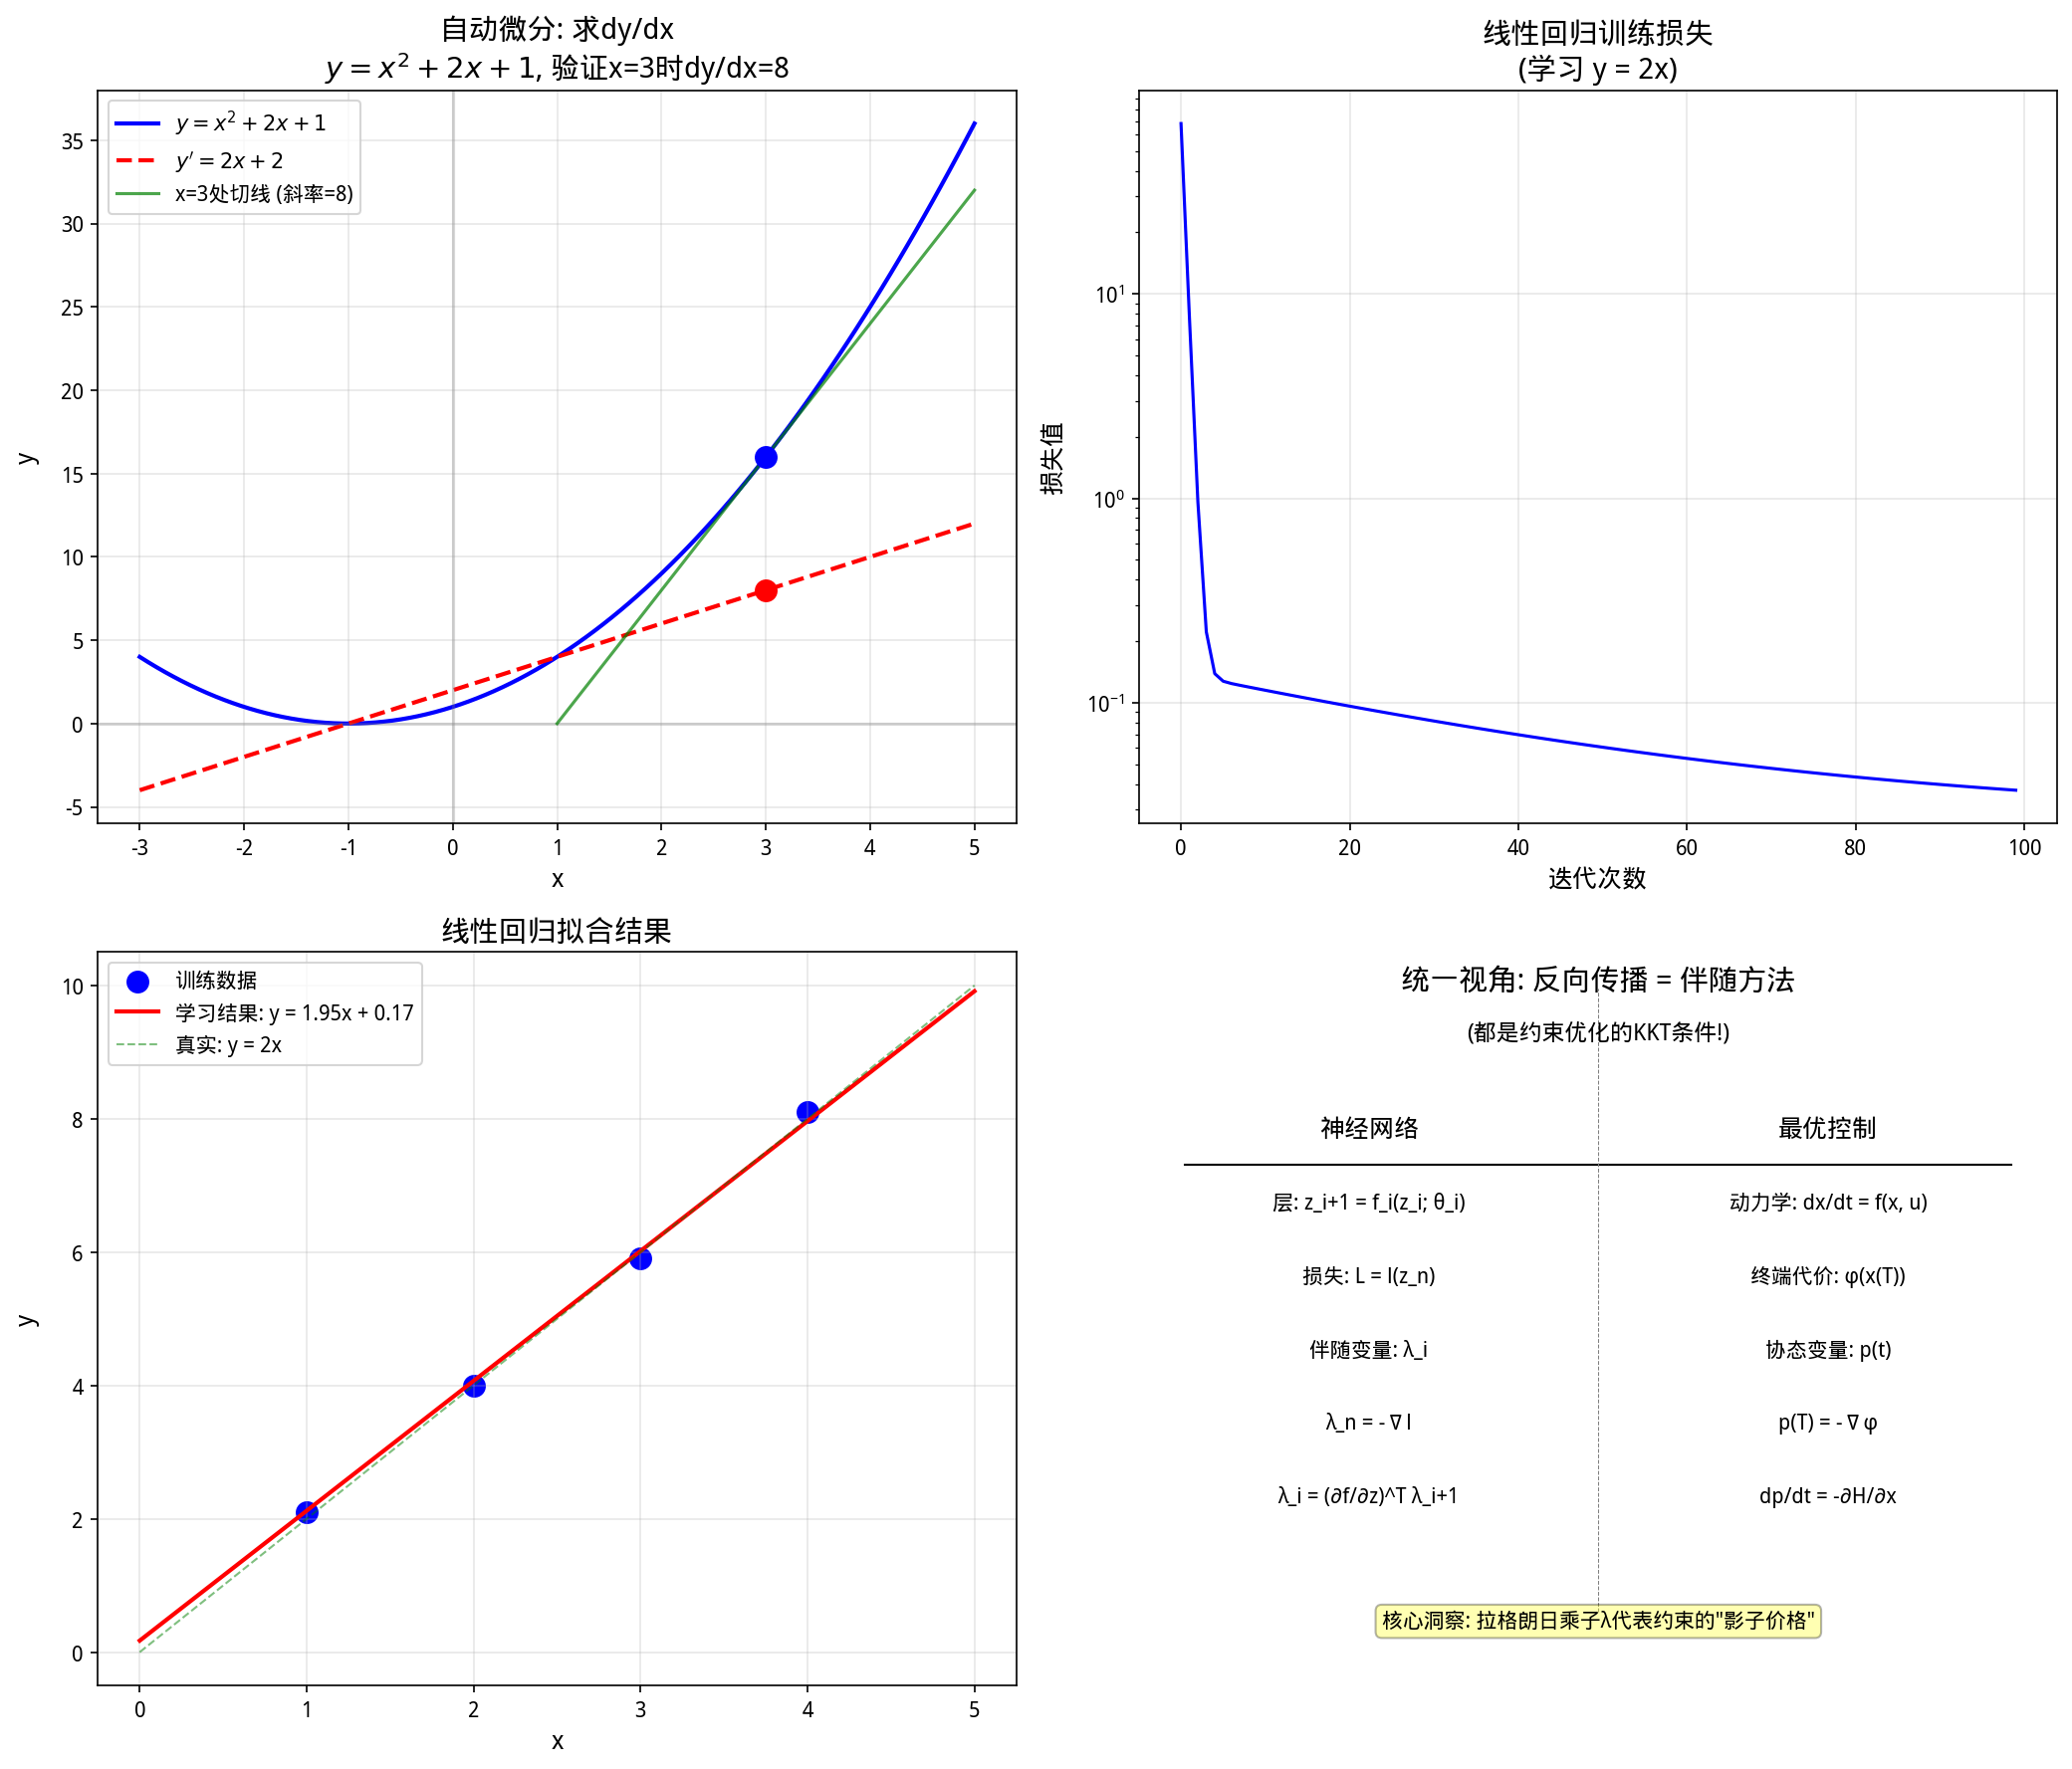
\includegraphics[width=0.95\textwidth]{figs_chap09/chap09_fig1.png}
\caption{自动微分与反向传播演示。（1）自动微分验证：本章例子 $y = x^2 + 2x + 1$，自动微分给出 $x = 3$ 处的切线斜率 $dy/dx = 8$，与手算一致；（2）用自动微分引擎训练线性回归 $y = 2x$ 的损失曲线；（3）拟合结果；（4）统一视角：神经网络的伴随变量 $\lambda_i$ 与最优控制的协态变量 $p(t)$ 逐项对应——都是约束优化的 KKT 条件。}
\label{fig:chap09_autograd}
\end{figure}

% ------------------------------------------------------------------------------------
\section{本章小结}

本章建立了深度学习与约束优化之间的桥梁：

\begin{enumerate}
    \item \textbf{神经网络}是一类参数化的复合函数，通过堆叠简单的线性变换和非线性激活来逼近复杂映射。
    
    \item \textbf{训练}是一个优化问题：最小化损失函数，找到最优参数。
    
    \item \textbf{计算图视角}：把复合函数展开为中间变量，每层变成一个等式约束。
    
    \item \textbf{拉格朗日函数}：引入乘子 $\lambda_i$，KKT条件给出伴随方程——这就是反向传播。
    
    \item \textbf{$\lambda_i$ 的意义}：第 $i$ 层输出对最终损失的敏感度，等价于``影子价格''。
    
    \item \textbf{统一框架}：反向传播 = 离散伴随方程 = 最优控制的数值版本。
\end{enumerate}

\begin{unification}[title=统一视角：伴随方法的三种面孔]
\begin{center}
\begin{tabular}{lll}
\toprule
\textbf{领域} & \textbf{正向过程} & \textbf{反向过程（伴随）} \\
\midrule
神经网络 & 前向传播 & 反向传播 \\
最优控制 & 状态方程 & 协态方程 \\
有限元/PDE & 求解原问题 & 敏感度分析 \\
\bottomrule
\end{tabular}
\end{center}
\end{unification}

\begin{physicalmeaning}
\textbf{$\lambda$ 在本章的意义}：$\lambda_i$ 是第 $i$ 层等式约束的影子价格——把第 $i$ 层的输出 $z_i$ 悄悄改动 $\epsilon$，最终损失变化 $-\lambda_i^\top \epsilon$。深度学习管 $\delta_i = -\lambda_i$ 叫"误差信号"，控制论管它叫"协态"，第1章管它叫"影子价格"——三个名字，一个东西。
\begin{itemize}
    \item 第8章：把"层 $i$"换成"时刻 $k$"、把参数 $\theta_i$ 换成控制 $u_k$，本章的伴随方程逐字变回第8章的离散伴随方程。
    \item 第10章：把损失换成"未来累计奖励"（符号因此翻转，$\lambda = +\partial J/\partial s$），把网络深度推到无穷，$\lambda$ 变成值函数的梯度，伴随方程变成贝尔曼方程。
    \item 第13章：把自动微分反过来用——不是对参数求导，而是对输入坐标 $(x, t)$ 求导，就能把偏微分方程本身写进损失函数（PINN）。
\end{itemize}
\end{physicalmeaning}

% ------------------------------------------------------------------------------------
\section{习题}

\paragraph{计算题}
\begin{enumerate}
    \item 考虑单层网络 $y = \sigma(Wx + b)$，损失 $L = \frac{1}{2}\|y - t\|^2$。
    \begin{enumerate}
        \item 写出拉格朗日函数。
        \item 推导 $\nabla_W L$ 和 $\nabla_b L$ 的表达式。
        \item 若 $\sigma(x) = \max(0, x)$（ReLU），写出梯度的具体形式。
    \end{enumerate}
    
    \item 对于softmax输出 $p_i = \frac{e^{z_i}}{\sum_j e^{z_j}}$ 和交叉熵损失 $L = -\sum_i y_i \log p_i$，证明 $\frac{\partial L}{\partial z_i} = p_i - y_i$。
    
    \item 考虑带skip connection的残差块：$z_{i+1} = z_i + f_i(z_i; \theta_i)$。推导它的伴随方程。
\end{enumerate}

\paragraph{编程题}
\begin{enumerate}
    \setcounter{enumi}{3}
    \item 扩展本章的自动微分引擎，添加以下运算：
    \begin{itemize}
        \item 矩阵乘法 $Y = XW$
        \item ReLU激活函数
        \item 交叉熵损失
    \end{itemize}
    
    \item 用你的引擎训练一个两层神经网络，在MNIST数据集的一个子集上进行手写数字分类。对比PyTorch的结果。
\end{enumerate}

\paragraph{思考题}
\begin{enumerate}
    \setcounter{enumi}{5}
    \item ``反向传播就是链式法则的应用''——这个常见说法有什么不准确之处？
    
    \item 为什么说反向传播是``空间换时间''的算法？它需要存储什么？
    
    \item 如果我们想计算二阶导数（Hessian矩阵），能否用类似的方法？这与``Hessian-free''优化有什么关系？
\end{enumerate}

\section*{扩展阅读：矩阵求导的规则与设计哲学}
\addcontentsline{toc}{section}{扩展阅读：矩阵求导}

在推导反向传播时，我们不可避免地要对矩阵、向量求导。这里系统介绍矩阵微积分的规则，更重要的是，解释\textbf{为什么}规则要这样设计。

\subsection*{核心问题：导数的``形状''应该是什么？}

考虑一个简单的问题：$y = Wx$，其中 $W \in \R^{m \times n}$，$x \in \R^n$，$y \in \R^m$。

问：$\frac{\partial y}{\partial x}$ 的形状应该是什么？

\textbf{直觉上}，$y$ 有 $m$ 个分量，$x$ 有 $n$ 个分量，所以导数应该有 $m \times n$ 个元素。但这 $m \times n$ 个元素应该排成什么形状？$m \times n$ 还是 $n \times m$？

这不是一个有唯一正确答案的问题——它是一个\textbf{约定}问题。不同的约定导致不同的``布局''（layout）。

\subsection*{两种布局约定}

\begin{definition}[雅可比矩阵的两种布局]
设 $f: \R^n \to \R^m$，即 $y = f(x)$，其中 $x \in \R^n$，$y \in \R^m$。

\textbf{分子布局}（Numerator Layout）：
\begin{equation}
\frac{\partial y}{\partial x} = \begin{pmatrix}
\frac{\partial y_1}{\partial x_1} & \frac{\partial y_1}{\partial x_2} & \cdots & \frac{\partial y_1}{\partial x_n} \\
\frac{\partial y_2}{\partial x_1} & \frac{\partial y_2}{\partial x_2} & \cdots & \frac{\partial y_2}{\partial x_n} \\
\vdots & \vdots & \ddots & \vdots \\
\frac{\partial y_m}{\partial x_1} & \frac{\partial y_m}{\partial x_2} & \cdots & \frac{\partial y_m}{\partial x_n}
\end{pmatrix} \in \R^{m \times n}
\end{equation}
第 $i$ 行第 $j$ 列是 $\frac{\partial y_i}{\partial x_j}$。行数跟分子走，列数跟分母走。

\textbf{分母布局}（Denominator Layout）：
\begin{equation}
\frac{\partial y}{\partial x} = \begin{pmatrix}
\frac{\partial y_1}{\partial x_1} & \frac{\partial y_2}{\partial x_1} & \cdots & \frac{\partial y_m}{\partial x_1} \\
\frac{\partial y_1}{\partial x_2} & \frac{\partial y_2}{\partial x_2} & \cdots & \frac{\partial y_m}{\partial x_2} \\
\vdots & \vdots & \ddots & \vdots \\
\frac{\partial y_1}{\partial x_n} & \frac{\partial y_2}{\partial x_n} & \cdots & \frac{\partial y_m}{\partial x_n}
\end{pmatrix} \in \R^{n \times m}
\end{equation}
就是分子布局的转置。行数跟分母走，列数跟分子走。
\end{definition}

\textbf{两种布局互为转置}，没有对错之分，只有方便与否。

\subsection*{为什么深度学习偏好分母布局？}

深度学习中，我们最关心的是\textbf{标量对向量的导数}：损失 $L$ 对参数 $\theta$ 的梯度。

设 $L \in \R$（标量），$\theta \in \R^n$（向量）。

\begin{itemize}
    \item \textbf{分子布局}：$\frac{\partial L}{\partial \theta} \in \R^{1 \times n}$（行向量）
    \item \textbf{分母布局}：$\frac{\partial L}{\partial \theta} \in \R^{n \times 1}$（列向量）
\end{itemize}

分母布局的好处是：\textbf{梯度和参数形状相同}。这样梯度下降可以直接写成：
\begin{equation}
\theta^{(t+1)} = \theta^{(t)} - \eta \nabla_\theta L
\end{equation}
不需要转置。PyTorch、TensorFlow 都采用这个约定。

\marginnote{\footnotesize
在深度学习框架里（PyTorch、TensorFlow、JAX），
参数 \texttt{w} 本身就是一个 \textbf{n×1 的张量}。
如果梯度也是 n×1，就可以直接做：

\texttt{w -= lr * w.grad}

而不用写
\texttt{w -= lr * w.grad.T}

越少转置，越少 bug。
}


\subsubsection*{一个最简单的例子（为什么分母布局更顺手？）}

深度学习中，最常见的梯度是 \textbf{标量损失 $L$ 对向量参数 $\theta$ 的导数}。

\[
L \in \mathbb{R}, \qquad \theta \in \mathbb{R}^n.
\]

两种常见定义是：

\begin{itemize}
    \item \textbf{分子布局（numerator layout）}：$\displaystyle \frac{\partial L}{\partial \theta} \in \mathbb{R}^{1 \times n}$（行向量）
    \item \textbf{分母布局（denominator layout）}：$\displaystyle \nabla_\theta L = \frac{\partial L}{\partial \theta} \in \mathbb{R}^{n \times 1}$（列向量）
\end{itemize}

深度学习框架（PyTorch / TensorFlow）统一采用分母布局，因为它使得梯度和参数形状一致，更新规则非常自然。

下面通过一个能够\textbf{直接代入数字手算}的例子来说明。

\paragraph{例子：最简单的线性模型}

设参数和输入为：

\[
x=\begin{pmatrix}2 \\ 3\end{pmatrix},\qquad 
w=\begin{pmatrix}1 \\ -1\end{pmatrix},\qquad 
t=4.
\]

模型输出：

\[
y = w^\top x = 1\cdot 2 + (-1)\cdot 3 = -1.
\]

平方误差损失：

\[
L=\frac12 (y - t)^2 = \frac12(-5)^2 = 12.5.
\]

\paragraph{计算梯度}

对于线性模型，损失对参数的梯度是：

\[
\nabla_w L = (y - t)\, x.
\]

代入数值：

\[
y - t = -1 - 4 = -5,
\qquad
x = \begin{pmatrix}2 \\ 3\end{pmatrix}.
\]

因此：

\[
\nabla_w L
= -5
\begin{pmatrix}2 \\ 3\end{pmatrix}
=
\begin{pmatrix}-10 \\ -15\end{pmatrix}.
\]

注意这是一个 \textbf{列向量}，与 $w$ 的形状完全一致。

\paragraph{梯度下降更新(手算)}

设学习率 $\eta=0.1$：

\[
w_{\text{new}}
= w - \eta \nabla_w L
=
\begin{pmatrix}1 \\ -1\end{pmatrix}
- 0.1
\begin{pmatrix}-10 \\ -15\end{pmatrix}
=
\begin{pmatrix}2 \\ 0.5\end{pmatrix}.
\]

完全不需要写转置！

\paragraph{如果用分子布局会怎样？}

分子布局得到的是行向量：

\[
\frac{\partial L}{\partial w} = [-10\ -15].
\]

更新必须写成：

\[
w_{\text{new}} = w - \eta \left( \frac{\partial L}{\partial w} \right)^{\top},
\]

否则维度不匹配（行向量 vs. 列向量）。

\bigskip
\begin{tcolorbox}[title=结论, colback=yellow!10!white]
深度学习采用分母布局（列向量梯度），因为它使得：

\[
\boxed{ \text{梯度和参数形状一致，更新公式无需转置，最自然。} }
\]

\end{tcolorbox}




\subsection*{标量对向量求导}

这是最基础的情况。设 $f: \R^n \to \R$，即 $y = f(x)$ 是标量。

\begin{keyformula}[title=标量对向量的梯度]
\begin{equation}
\nabla_x f = \frac{\partial f}{\partial x} = \begin{pmatrix}
\frac{\partial f}{\partial x_1} \\
\frac{\partial f}{\partial x_2} \\
\vdots \\
\frac{\partial f}{\partial x_n}
\end{pmatrix} \in \R^n
\end{equation}
（分母布局：梯度是列向量，与 $x$ 形状相同）
\end{keyformula}

\textbf{常用公式}：
\begin{align}
\nabla_x (a^\top x) &= a \\
\nabla_x (x^\top A x) &= (A + A^\top) x \\
\nabla_x \|x\|^2 &= 2x \\
\nabla_x \|Ax - b\|^2 &= 2A^\top(Ax - b)
\end{align}

\subsection*{标量对矩阵求导}

设 $f: \R^{m \times n} \to \R$，即 $y = f(X)$ 是标量，$X$ 是矩阵。

\begin{keyformula}[title=标量对矩阵的梯度]
\begin{equation}
\nabla_X f = \frac{\partial f}{\partial X} = \begin{pmatrix}
\frac{\partial f}{\partial X_{11}} & \frac{\partial f}{\partial X_{12}} & \cdots \\
\frac{\partial f}{\partial X_{21}} & \frac{\partial f}{\partial X_{22}} & \cdots \\
\vdots & \vdots & \ddots
\end{pmatrix} \in \R^{m \times n}
\end{equation}
梯度矩阵与 $X$ 形状相同，第 $(i,j)$ 元素是 $\frac{\partial f}{\partial X_{ij}}$。
\end{keyformula}

\textbf{常用公式}：
\begin{align}
\nabla_X \tr(AX) &= A^\top \\
\nabla_X \tr(X^\top A) &= A \\
\nabla_X \tr(AXB) &= A^\top B^\top \\
\nabla_X \tr(X^\top AX) &= (A + A^\top)X \\
\nabla_X (a^\top X b) &= ab^\top
\end{align}

\marginnote{这些公式看起来复杂，但都可以通过``展开成分量，求导，再组装回去''的方法推导。关键是保持布局一致。}

\subsection*{向量对向量求导（雅可比矩阵）}

设 $f: \R^n \to \R^m$，即 $y = f(x)$，其中 $y \in \R^m$，$x \in \R^n$。

\begin{keyformula}[title=雅可比矩阵]
分子布局下：
\begin{equation}
J = \frac{\partial y}{\partial x} = \begin{pmatrix}
\frac{\partial y_1}{\partial x_1} & \cdots & \frac{\partial y_1}{\partial x_n} \\
\vdots & \ddots & \vdots \\
\frac{\partial y_m}{\partial x_1} & \cdots & \frac{\partial y_m}{\partial x_n}
\end{pmatrix} \in \R^{m \times n}
\end{equation}
第 $i$ 行是 $\nabla_{x} y_i$ 的转置。
\end{keyformula}

\textbf{常用公式}：
\begin{align}
\frac{\partial (Ax)}{\partial x} &= A \quad \text{（$A$ 是常矩阵）} \\
\frac{\partial (Ax)}{\partial A} &= ? \quad \text{（这需要更复杂的记号，见下文）}
\end{align}

\subsection*{神经网络中的关键公式}

在反向传播中，我们最常遇到的是以下几种情况：

\textbf{情况1}：$z = Wx + b$，求 $\frac{\partial L}{\partial W}$

设 $L$ 是标量损失，$\delta = \frac{\partial L}{\partial z}$ 已知（从后面传回来的梯度）。

\begin{equation}
\boxed{\frac{\partial L}{\partial W} = \delta \, x^\top}
\end{equation}

\textbf{推导}：用链式法则，$L$ 通过 $z$ 依赖于 $W$。
\begin{equation}
\frac{\partial L}{\partial W_{ij}} = \sum_k \frac{\partial L}{\partial z_k} \frac{\partial z_k}{\partial W_{ij}} = \frac{\partial L}{\partial z_i} \cdot x_j = \delta_i x_j
\end{equation}
组装成矩阵形式就是 $\delta x^\top$。

\textbf{情况2}：$z = Wx$，求 $\frac{\partial L}{\partial x}$（传给上一层的梯度）

\begin{equation}
\boxed{\frac{\partial L}{\partial x} = W^\top \delta}
\end{equation}

\textbf{推导}：
\begin{equation}
\frac{\partial L}{\partial x_j} = \sum_k \frac{\partial L}{\partial z_k} \frac{\partial z_k}{\partial x_j} = \sum_k \delta_k W_{kj} = (W^\top \delta)_j
\end{equation}

\textbf{情况3}：$z = \sigma(a)$（逐元素激活），求 $\frac{\partial L}{\partial a}$

\begin{equation}
\boxed{\frac{\partial L}{\partial a} = \delta \odot \sigma'(a)}
\end{equation}

其中 $\odot$ 是逐元素乘法（Hadamard积），$\sigma'(a)$ 是激活函数的导数逐元素作用于 $a$。

\subsection*{为什么转置会出现？}

很多初学者困惑：为什么 $\frac{\partial L}{\partial x} = W^\top \delta$ 要有转置？

\textbf{直觉解释}：前向传播时，$W$ 把 $n$ 维空间映射到 $m$ 维空间。反向传播时，梯度要从 $m$ 维空间``映射回'' $n$ 维空间。这个``反向映射''就是 $W^\top$。

\textbf{更深的理解}：$W^\top$ 是 $W$ 的\textbf{伴随算子}（adjoint）。在内积空间中，线性算子 $A$ 的伴随 $A^*$ 满足 $\langle Ax, y \rangle = \langle x, A^* y \rangle$。对于实矩阵，伴随就是转置。

这解释了为什么伴随方程（反向传播）中到处是转置——它们在数学上是前向算子的伴随。

\subsection*{记忆技巧：维度分析}

当你不确定某个公式时，\textbf{维度分析}是最可靠的检验：

\begin{itemize}
    \item $W \in \R^{m \times n}$，$x \in \R^n$，则 $Wx \in \R^m$ ✓
    \item $\delta \in \R^m$（与 $z$ 同形状），$x \in \R^n$
    \item $\frac{\partial L}{\partial W}$ 应与 $W$ 同形状，即 $\R^{m \times n}$
    \item $\delta x^\top \in \R^{m \times 1} \cdot \R^{1 \times n} = \R^{m \times n}$ ✓
\end{itemize}

\begin{insightbox}[title=实用建议]
\begin{enumerate}
    \item \textbf{坚持一种布局}：推荐分母布局（梯度与变量同形状）。
    \item \textbf{标量是安全的}：遇到复杂情况，先把 $L$ 写成标量形式，对每个分量求导，再组装。
    \item \textbf{维度检验}：每一步都检查维度是否匹配。
    \item \textbf{用迹的技巧}：$a^\top X b = \tr(ab^\top X^\top) = \tr(b a^\top X)$，迹对矩阵求导有简洁公式。
\end{enumerate}
\end{insightbox}

\subsection*{与拉格朗日方法的联系}

回到本章的主题：为什么拉格朗日方法能避免矩阵求导的混乱？

关键在于：\textbf{拉格朗日函数 $\mathcal{L}$ 是标量}。

当我们写：
\begin{equation}
\mathcal{L} = L(z_n) + \sum_i \lambda_i^\top (z_i - f_i(z_{i-1}; W_i))
\end{equation}

每一项都是标量（$\lambda_i^\top (\cdots)$ 是向量内积，结果是标量）。对标量求导：
\begin{itemize}
    \item 对向量求导 → 得到同形状的向量
    \item 对矩阵求导 → 得到同形状的矩阵
\end{itemize}

不需要处理雅可比矩阵、三阶张量这些复杂对象。转置符号也会从标量求导的规则中\textbf{自动出现}，而不需要我们去猜。

这就是拉格朗日方法的优雅之处：它把高维的矩阵微积分问题，降维成了一系列标量微积分问题。


\section*{扩展阅读：Python 如何理解 \texttt{x * x + x * 2 + 1}？}
\addcontentsline{toc}{section}{扩展阅读：Python表达式求值}

\marginnote{这一节解释 Python 解释器的工作原理。理解这个，你就明白了为什么我们只需要重载运算符，就能``免费''获得计算图构建的能力。}

当我们写下 \texttt{y = x * x + x * 2 + 1} 时，Python 解释器究竟做了什么？为什么它知道``先乘后加''？

\subsection*{三步走：从源代码到执行结果}

Python 执行这行代码，实际上经历了三个阶段：

\paragraph{第一步：解析（Parsing）—— 读懂表达式结构}

Python 按照数学规则（先乘除后加减，同级从左到右），把源代码解析成一棵\textbf{抽象语法树}（Abstract Syntax Tree, AST）：

\begin{center}
\begin{tikzpicture}[
    level distance=1.2cm,
    sibling distance=2cm,
    every node/.style={draw, circle, minimum size=0.8cm, font=\small},
    edge from parent/.style={draw, ->, thick}
]
    \node {$+$}
        child { node {$+$}
            child { node {$\times$}
                child { node {$x$} }
                child { node {$x$} }
            }
            child { node {$\times$}
                child { node {$x$} }
                child { node {$2$} }
            }
        }
        child { node {$1$} };
\end{tikzpicture}
\end{center}

这棵树的结构就是 $(((x \times x) + (x \times 2)) + 1)$。\textbf{``先乘后加''是在这一步决定的}。

\paragraph{第二步：编译（Compilation）—— 把树变成指令序列}

Python 编译器把 AST 翻译成一串\textbf{字节码指令}（bytecode）。每条指令只做一件很小的事：

\begin{center}
\renewcommand{\arraystretch}{1.3}
\begin{tabular}{cl}
\toprule
\textbf{指令} & \textbf{含义} \\
\midrule
\texttt{LOAD\_FAST x} & 把变量 $x$ 压入栈顶 \\
\texttt{BINARY\_MULTIPLY} & 弹出栈顶两个数，相乘，结果压回栈顶 \\
\texttt{BINARY\_ADD} & 弹出栈顶两个数，相加，结果压回栈顶 \\
\texttt{LOAD\_CONST 2} & 把常数 2 压入栈顶 \\
\bottomrule
\end{tabular}
\end{center}

\paragraph{第三步：执行（Execution）—— 用栈依次运行指令}

解释器维护一个\textbf{栈}（像一摞盘子），严格按字节码顺序执行：

\begin{center}
\renewcommand{\arraystretch}{1.4}
\begin{tabular}{c|l|l}
\toprule
\textbf{步骤} & \textbf{执行的指令} & \textbf{栈的状态}（右边是栈顶） \\
\midrule
1 & \texttt{LOAD\_FAST x} & $[3.0]$ \\
2 & \texttt{LOAD\_FAST x} & $[3.0, 3.0]$ \\
3 & \texttt{BINARY\_MULTIPLY} $\to$ 调用 \texttt{x.\_\_mul\_\_(x)} & $[m_1]$ \quad ($m_1$.data=9.0) \\
\midrule
4 & \texttt{LOAD\_FAST x} & $[m_1, 3.0]$ \\
5 & \texttt{LOAD\_CONST 2} & $[m_1, 3.0, 2]$ \\
6 & \texttt{BINARY\_MULTIPLY} $\to$ 调用 \texttt{x.\_\_mul\_\_(2)} & $[m_1, m_2]$ \quad ($m_2$.data=6.0) \\
\midrule
7 & \texttt{BINARY\_ADD} $\to$ 调用 \texttt{m1.\_\_add\_\_(m2)} & $[s_1]$ \quad ($s_1$.data=15.0) \\
\midrule
8 & \texttt{LOAD\_CONST 1} & $[s_1, 1]$ \\
9 & \texttt{BINARY\_ADD} $\to$ 调用 \texttt{s1.\_\_add\_\_(1)} & $[y]$ \quad ($y$.data=16.0) \\
\bottomrule
\end{tabular}
\end{center}

\textbf{关键洞察}：每次执行 \texttt{BINARY\_MULTIPLY} 或 \texttt{BINARY\_ADD} 时，Python 会调用我们重载的 \texttt{\_\_mul\_\_} 或 \texttt{\_\_add\_\_} 方法。在这些方法里，我们不仅计算了数值，还\textbf{顺便}创建了计算图节点！

\subsection*{真的可以看到字节码吗？}

可以！Python 提供了 \texttt{dis} 模块来查看字节码：

\begin{lstlisting}[style=teaching, language=Python]
import dis

def f(x):
    return x * x + x * 2 + 1

dis.dis(f)
\end{lstlisting}

输出（简化后）：

\begin{lstlisting}[style=teaching, language=Python, numbers=none]
  3           0 LOAD_FAST                0 (x)
              2 LOAD_FAST                0 (x)
              4 BINARY_MULTIPLY              # x * x -> m1

              6 LOAD_FAST                0 (x)
              8 LOAD_CONST               1 (2)
             10 BINARY_MULTIPLY              # x * 2 -> m2

             12 BINARY_ADD                   # m1 + m2 -> s1

             14 LOAD_CONST               2 (1)
             16 BINARY_ADD                   # s1 + 1 -> y

             18 RETURN_VALUE
\end{lstlisting}

这正是我们前面 Step 1--4 图的``官方版本''！

\subsection*{小结}

\begin{center}
\begin{tikzpicture}[
    box/.style={draw, rounded corners, minimum width=3cm, minimum height=1cm, font=\small, align=center},
    arrow/.style={->, thick, >=stealth}
]
    \node[box, fill=blue!10] (src) at (0, 0) {源代码\\{\ttfamily x*x + x*2 + 1}};
    \node[box, fill=green!10] (ast) at (4.5, 0) {抽象语法树\\（确定优先级）};
    \node[box, fill=yellow!10] (bc) at (9, 0) {字节码序列\\（线性指令）};
    \node[box, fill=red!10] (exec) at (13.5, 0) {栈式执行\\（调用重载方法）};
    
    \draw[arrow] (src) -- node[above, font=\scriptsize] {解析} (ast);
    \draw[arrow] (ast) -- node[above, font=\scriptsize] {编译} (bc);
    \draw[arrow] (bc) -- node[above, font=\scriptsize] {执行} (exec);
\end{tikzpicture}
\end{center}

\begin{itemize}
    \item \textbf{``先乘后加''}是在\textbf{解析阶段}决定的（构建 AST）
    \item \textbf{``从左到右''}是在\textbf{执行阶段}实现的（按字节码顺序）
    \item \textbf{我们没有写任何解析器}，Python 帮我们做完了所有这些工作
    \item 我们只需要\textbf{重载运算符}，就能在执行阶段``搭便车''构建计算图
\end{itemize}

这就是自动微分框架的设计哲学：\textbf{利用宿主语言的表达式求值机制，免费获得计算图构建能力}。PyTorch、JAX、TensorFlow Eager 都是这个思路。

\section*{扩展阅读：深度学习与数值方法的深刻联系——第5章的后续}
\addcontentsline{toc}{section}{扩展阅读：与数值方法的联系}

\marginnote{这一节揭示深度学习与经典数值方法的内在联系。你会发现，很多``新''的深度学习技术，其实是老方法的新面孔。}

深度学习中的许多核心概念，与数值线性代数、有限元方法有着惊人的相似性。理解这些联系，能帮助你更深刻地理解两个领域。

\subsection*{条件数与训练困难}

梯度下降的收敛速度取决于损失函数的\textbf{Hessian矩阵}（二阶导数矩阵）的\textbf{条件数}。

\begin{definition}[Hessian 矩阵]
Hessian 矩阵 $H$ 是损失函数的二阶偏导数组成的矩阵：
\begin{equation}
H_{ij} = \frac{\partial^2 L}{\partial \theta_i \partial \theta_j}
\end{equation}
它描述了损失曲面的``曲率''——在不同方向上曲面弯曲的程度。
\end{definition}

\begin{figure}[h]
\centering
\begin{tikzpicture}[scale=0.75]
    % 良态：接近圆形
    \begin{scope}
        \node[font=\bfseries] at (2, 3.8) {良态（$\kappa \approx 1$）};
        \draw[->] (0, 0) -- (4, 0) node[right] {$\theta_1$};
        \draw[->] (0, 0) -- (0, 3.2) node[above] {$\theta_2$};
        
        % 等高线（接近圆形）
        \draw[blue!40] (2, 1.5) ellipse (1.4 and 1.2);
        \draw[blue!60] (2, 1.5) ellipse (0.9 and 0.75);
        \draw[blue!80] (2, 1.5) ellipse (0.4 and 0.33);
        \fill[red] (2, 1.5) circle (2pt);
        
        % 梯度下降路径
        \draw[->, thick, red] (0.8, 2.5) -- (1.5, 1.8) -- (1.9, 1.55) -- (2, 1.5);
        
        \node[font=\small] at (2, -0.5) {各方向曲率相近 $\to$ 快速收敛};
    \end{scope}
    
    % 病态：扁椭圆
    \begin{scope}[xshift=6.5cm]
        \node[font=\bfseries] at (2, 3.8) {病态（$\kappa \gg 1$）};
        \draw[->] (0, 0) -- (4, 0) node[right] {$\theta_1$};
        \draw[->] (0, 0) -- (0, 3.2) node[above] {$\theta_2$};
        
        % 等高线（扁椭圆）
        \draw[blue!40, rotate around={20:(2,1.5)}] (2, 1.5) ellipse (1.6 and 0.35);
        \draw[blue!60, rotate around={20:(2,1.5)}] (2, 1.5) ellipse (1.0 and 0.22);
        \draw[blue!80, rotate around={20:(2,1.5)}] (2, 1.5) ellipse (0.4 and 0.09);
        \fill[red] (2, 1.5) circle (2pt);
        
        % 梯度下降路径（锯齿）
        \draw[->, thick, red] (3.5, 2.3) -- (2.5, 1.2) -- (3.0, 1.7) -- (2.3, 1.3) -- (2.6, 1.55) -- (2.2, 1.4);
        
        \node[font=\small] at (2, -0.5) {曲率差异大 $\to$ 锯齿震荡};
    \end{scope}
\end{tikzpicture}
\caption{条件数决定损失曲面的``形状''：圆形容易优化，扁椭圆困难}
\end{figure}

\begin{itemize}
    \item \textbf{$\kappa$ 小}：各方向曲率相近，等高线接近圆形，梯度直指最低点
    \item \textbf{$\kappa$ 大}：有的方向很陡，有的方向很平，梯度下降会在陡峭方向来回震荡
\end{itemize}

这与求解线性方程组 $Ax = b$ 时的情况完全一致！

\subsection*{优化器 = 预条件子}

几乎所有现代优化器都可以理解为某种\textbf{预条件}（preconditioning）！

\begin{center}
\renewcommand{\arraystretch}{1.4}
\begin{tabular}{l|l|l}
\toprule
\textbf{数值线性代数} & \textbf{深度学习优化器} & \textbf{预条件矩阵 $M$} \\
\midrule
无预条件 & SGD & $M = I$ \\
Jacobi 预条件 & Adagrad / RMSprop & $M = \text{diag}(\sqrt{v})$ \\
近似 Newton 法 & Adam & $M = \text{diag}(\sqrt{\hat{v}})$ \\
完整 Newton 法 & K-FAC, Shampoo & $M \approx H$ \\
\bottomrule
\end{tabular}
\end{center}

\textbf{Adam 的本质}：用对角预条件子对梯度进行缩放：
\begin{equation}
\theta^{(t+1)} = \theta^{(t)} - \eta \cdot \frac{\hat{m}}{\sqrt{\hat{v}} + \epsilon} = \theta^{(t)} - \eta \cdot M^{-1} \hat{m}
\end{equation}

\begin{itemize}
    \item 梯度大的方向（$\hat{v}$ 大）：步长缩小，防止震荡
    \item 梯度小的方向（$\hat{v}$ 小）：步长放大，加速收敛
\end{itemize}

这与数值线性代数中的 Jacobi 预条件思想完全一致！

\subsection*{稀疏性：从有限元到卷积网络}

有限元刚度矩阵是\textbf{稀疏}的（每个节点只与邻居耦合），现代神经网络也追求稀疏性。

\begin{figure}[h]
\centering
\begin{tikzpicture}[scale=0.8]
    % 左边：全连接
    \begin{scope}
        \node[font=\bfseries] at (1.5, 4) {全连接层};
        % 输入节点
        \foreach \i in {1,...,4} {
            \fill[blue] (0, \i) circle (4pt);
        }
        % 输出节点
        \foreach \i in {1,...,3} {
            \fill[red] (3, \i+0.5) circle (4pt);
        }
        % 连接
        \foreach \i in {1,...,4} {
            \foreach \j in {1,...,3} {
                \draw[gray, thin] (0, \i) -- (3, \j+0.5);
            }
        }
        \node[font=\small] at (1.5, 0.3) {$O(n \times m)$ 参数};
    \end{scope}
    
    % 右边：稀疏连接（卷积）
    \begin{scope}[xshift=6cm]
        \node[font=\bfseries] at (1.5, 4) {卷积层};
        % 输入节点
        \foreach \i in {1,...,4} {
            \fill[blue] (0, \i) circle (4pt);
        }
        % 输出节点
        \foreach \i in {1,...,3} {
            \fill[red] (3, \i+0.5) circle (4pt);
        }
        % 局部连接
        \draw[thick] (0, 1) -- (3, 1.5);
        \draw[thick] (0, 2) -- (3, 1.5);
        \draw[thick] (0, 2) -- (3, 2.5);
        \draw[thick] (0, 3) -- (3, 2.5);
        \draw[thick] (0, 3) -- (3, 3.5);
        \draw[thick] (0, 4) -- (3, 3.5);
        \node[font=\small] at (1.5, 0.3) {$O(k)$ 参数};
    \end{scope}
\end{tikzpicture}
\caption{全连接层 vs 卷积层：稀疏连接大幅减少参数}
\end{figure}

\textbf{卷积神经网络（CNN）}利用了与有限元相同的原理：

\begin{itemize}
    \item \textbf{局部连接}：每个输出只依赖局部输入（类比：每个节点只与邻居耦合）
    \item \textbf{权值共享}：不同位置用相同的卷积核（类比：均匀网格上的单元刚度矩阵相同）
    \item \textbf{稀疏性}：参数量从 $O(n^2)$ 降到 $O(n)$
\end{itemize}

\begin{insightbox}[title=局部性的力量]
有限元方法和卷积神经网络都在利用\textbf{局部性}——物理世界的大多数相互作用是局部的：
\begin{itemize}
    \item 热量从高温流向低温（局部传导）
    \item 力通过接触传递（局部作用）
    \item 图像特征是局部的（边缘、纹理）
\end{itemize}
局部性导致稀疏结构，稀疏结构带来计算上的巨大节省！
\end{insightbox}

\subsection*{多重网格与 U-Net}

数值方法中的\textbf{多重网格}（multigrid）技术在深度学习中有惊人的对应物：\textbf{U-Net}！

\begin{figure}[h]
\centering
\begin{tikzpicture}[scale=0.65]
    % U-Net 结构
    % 左边：编码器（下采样）
    \draw[fill=blue!30] (0, 0) rectangle (1.5, 4);
    \node[font=\scriptsize] at (0.75, 2) {细};
    \draw[fill=blue!40] (2, 0.5) rectangle (3, 3.5);
    \draw[fill=blue!50] (3.5, 1) rectangle (4.5, 3);
    \draw[fill=blue!60] (5, 1.5) rectangle (5.5, 2.5);
    \node[font=\scriptsize] at (5.25, 2) {粗};
    
    % 右边：解码器（上采样）
    \draw[fill=red!30] (9, 0) rectangle (10.5, 4);
    \node[font=\scriptsize] at (9.75, 2) {细};
    \draw[fill=red!40] (7.5, 0.5) rectangle (8.5, 3.5);
    \draw[fill=red!50] (6, 1) rectangle (7, 3);
    
    % 跳跃连接
    \draw[->, thick, green!60!black] (1.5, 3.5) to[bend left=20] (9, 3.5);
    \draw[->, thick, green!60!black] (3, 3) to[bend left=15] (7.5, 3);
    \draw[->, thick, green!60!black] (4.5, 2.5) to[bend left=10] (6, 2.5);
    
    % 箭头
    \draw[->, thick] (1.6, 2) -- (1.9, 2);
    \draw[->, thick] (3.1, 2) -- (3.4, 2);
    \draw[->, thick] (4.6, 2) -- (4.9, 2);
    \draw[->, thick] (5.6, 2) -- (5.9, 2);
    \draw[->, thick] (7.1, 2) -- (7.4, 2);
    \draw[->, thick] (8.6, 2) -- (8.9, 2);
    
    % 标签
    \node at (2.5, 4.8) {下采样（限制）};
    \node at (7.5, 4.8) {上采样（插值）};
    \node[green!60!black, font=\small] at (5.25, 4.3) {跳跃连接};
\end{tikzpicture}
\caption{U-Net 结构与多重网格的惊人相似}
\end{figure}

\begin{center}
\renewcommand{\arraystretch}{1.4}
\begin{tabular}{l|l}
\toprule
\textbf{多重网格} & \textbf{U-Net} \\
\midrule
限制（Restriction） & 池化 / 下采样 \\
粗网格求解 & 瓶颈层处理 \\
插值（Prolongation） & 转置卷积 / 上采样 \\
粗细网格信息传递 & 跳跃连接（Skip Connection） \\
\bottomrule
\end{tabular}
\end{center}

U-Net 在医学图像分割等任务中非常成功——它继承了多重网格``多尺度处理''的智慧！

\subsection*{GPU 并行：为什么深度学习需要 GPU}

深度学习的爆发离不开 \textbf{GPU}，而 GPU 擅长的恰恰是\textbf{大规模并行计算}。

\begin{figure}[h]
\centering
\begin{tikzpicture}[scale=0.8]
    % CPU
    \begin{scope}
        \node[font=\bfseries] at (1.6, 2.8) {CPU};
        \foreach \i in {0,...,3} {
            \draw[fill=blue!50] (\i*0.8, 0) rectangle ++(0.7, 0.7);
        }
        \node[font=\small] at (1.6, -0.5) {4--16 个强核心};
        \node[font=\small] at (1.6, -1) {擅长复杂逻辑};
    \end{scope}
    
    % GPU
    \begin{scope}[xshift=6cm]
        \node[font=\bfseries] at (2.4, 2.8) {GPU};
        \foreach \i in {0,...,9} {
            \foreach \j in {0,...,3} {
                \draw[fill=green!50] (\i*0.5, \j*0.5) rectangle ++(0.4, 0.4);
            }
        }
        \node[font=\small] at (2.4, -0.5) {数千个小核心};
        \node[font=\small] at (2.4, -1) {擅长简单并行};
    \end{scope}
\end{tikzpicture}
\caption{CPU vs GPU：不同的设计哲学}
\end{figure}

\textbf{为什么神经网络适合 GPU？}

神经网络的核心运算是\textbf{矩阵乘法}：$Y = XW + b$。

矩阵乘法中，每个输出元素 $Y_{ij} = \sum_k X_{ik} W_{kj}$ 可以\textbf{独立计算}——这是天然的并行结构！

\begin{insightbox}[title=GPU 友好的计算模式]
\begin{enumerate}
    \item \textbf{大量独立的相同操作}（如 batch 中每个样本的前向传播）
    \item \textbf{规则的内存访问}（如矩阵乘法的连续读写）
    \item \textbf{少量分支逻辑}（避免 if-else 导致的线程分化）
\end{enumerate}

这解释了为什么：
\begin{itemize}
    \item Transformer 比 RNN 更容易并行（无时序依赖）
    \item 卷积比全连接更高效（局部性好，缓存友好）
    \item Batch Normalization 比 Layer Normalization 更 GPU 友好
\end{itemize}
\end{insightbox}

\subsection*{统一的视角}

回顾本章和这些扩展阅读，我们看到一个统一的图景：

\begin{center}
\renewcommand{\arraystretch}{1.5}
\begin{tabular}{l|l|l}
\toprule
\textbf{概念} & \textbf{数值方法} & \textbf{深度学习} \\
\midrule
核心问题 & 求解 $Ax = b$ 或 $\min_x f(x)$ & 求解 $\min_\theta L(\theta)$ \\
迭代方法 & Jacobi, Gauss-Seidel, CG & SGD, Momentum, Adam \\
加速技术 & 预条件子 & 自适应学习率 \\
利用结构 & 稀疏矩阵 & 卷积、注意力 \\
多尺度 & 多重网格 & U-Net, Feature Pyramid \\
并行化 & 区域分解 & 数据并行、模型并行 \\
\bottomrule
\end{tabular}
\end{center}

\textbf{核心信息}：深度学习不是凭空出现的``黑魔法''，而是建立在几十年数值计算研究基础上的自然延伸。理解经典方法，能帮助你更好地理解和改进现代深度学习技术。

\section*{扩展阅读：深度学习的计算基础设施}
\addcontentsline{toc}{section}{扩展阅读：计算基础设施}

当你写下 \texttt{y = torch.matmul(A, B)} 时，背后发生了什么？为什么 GPU 
比 CPU 快 100 倍？为了理解这一点，我们先从一个经典的小故事开始。

\subsection*{一个被认为“毫无意义”的实验}

\marginnote{\textbf{Geoffrey Hinton}(1947--)：``深度学习教父''，2018年图灵奖得主。他在多伦多大学坚持神经网络研究三十年，在AI冬天时几乎是孤军奋战。2012年AlexNet的成功证明了他的坚持。2023年他辞去Google职位，公开警告AI的潜在危险。}

2009 年，Montreal 的一间小实验室里，博士生 Ranzato、
助手 Alex Krizhevsky，以及他们的导师 Hinton 正在做一个
很多人看来``一点用都没有''的实验——

\begin{quote}
用当时游戏玩家的显卡（NVIDIA GTX 280）来训练一个
卷积神经网络。
\end{quote}

在那个年代，深度学习还远没有今天的气势。主流观点认为：

\begin{itemize}
    \item 深度网络太大，训练太慢；
    \item GPU 只是玩游戏的，没有科研价值；
    \item 机器学习的未来应该是从数学上给模型加约束，而不是暴力堆算力。
\end{itemize}

但 Krizhevsky 注意到了一件别人忽略的事：  
游戏显卡的核心结构（SIMD + 大量并行浮点单元）和卷积操作的数学结构是完美匹配的。

于是他们写下了第一版用 CUDA 加速卷积的代码，
发现速度比 CPU \textbf{快了几十倍}。Hinton 后来回忆说：

\begin{quote}
``第一次看到 GPU 把卷积层跑得这么快时，我们觉得好像未来突然被打开了。''
\end{quote}

三年后，也就是 2012 年，Krizhevsky 基于这些经验写出了 \texttt{cuda-convnet}，并用一台双 GTX 580 显卡训练出了历史性的模型——

\begin{center}
\textbf{AlexNet}
\end{center}

它把 ImageNet 错误率降低了 10 个百分点，直接点燃了整个深度学习时代。

从此之后，一个事实被彻底确认：

\begin{quote}
\textbf{深度学习的突破，离不开硬件架构与数学结构的完美匹配。}
\end{quote}

而你今天执行的 \texttt{torch.matmul}、\texttt{conv2d} 等操作，
本质上都是在 GPU 上调用几十年积累下来的线性代数内核（cuBLAS、cuDNN），
这些内核又精确地利用了 GPU 的大规模并行结构。

因此，表面上一行 Python：

\begin{equation}
y = \text{torch.matmul}(A, B)
\end{equation}

背后是一整套工业级的软硬件生态：计算图编译器、Tensor Core、
warp 调度、内存对齐、缓存优化、并行线程块调度……

理解这一点后，PyTorch 为什么快，就不再是魔法，而是工程与数学共同的必然结果(这一节以英伟达NVIDIA相关生态举例，华为等硬件厂商也有类似的底层架构逻辑，机器码和线程管理模式不尽相同)。

\subsection*{GPU 编程的层次结构}

深度学习的计算栈是这样的：

\begin{figure}[h]
\centering
\begin{tikzpicture}[
    box/.style={draw, rounded corners, minimum width=4cm, minimum height=0.9cm, font=\small, align=center},
    arrow/.style={->, thick, >=stealth}
]
    \node[box, fill=blue!20] (python) at (0, 5) {Python 代码\\{\ttfamily y = model(x)}};
    \node[box, fill=blue!30] (pytorch) at (0, 3.8) {PyTorch / JAX / TensorFlow\\自动微分、张量操作};
    \node[box, fill=green!20] (cuda) at (0, 2.6) {CUDA / cuDNN / cuBLAS\\GPU 算子库};
    \node[box, fill=yellow!20] (driver) at (0, 1.4) {GPU 驱动\\内存管理、任务调度};
    \node[box, fill=red!20] (hw) at (0, 0.2) {GPU 硬件\\CUDA Core / Tensor Core};
    
    \draw[arrow] (python) -- (pytorch);
    \draw[arrow] (pytorch) -- (cuda);
    \draw[arrow] (cuda) -- (driver);
    \draw[arrow] (driver) -- (hw);
    
    % 右侧标注
    \node[right, font=\small, text=gray] at (2.3, 5) {你写的};
    \node[right, font=\small, text=gray] at (2.3, 3.8) {框架提供};
    \node[right, font=\small, text=gray] at (2.3, 2.6) {NVIDIA 提供};
    \node[right, font=\small, text=gray] at (2.3, 1.4) {系统层};
    \node[right, font=\small, text=gray] at (2.3, 0.2) {硬件层};
\end{tikzpicture}
\caption{深度学习计算栈：从 Python 到硬件}
\end{figure}

\subsection*{CUDA：GPU 编程的基础}

\textbf{CUDA}（Compute Unified Device Architecture）是 NVIDIA 的 GPU 编程平台。

\paragraph{核心概念}

\begin{itemize}
    \item \textbf{Thread}：最小执行单元，执行相同的代码（SIMT: Single Instruction Multiple Threads）
    \item \textbf{Block}：一组线程，共享高速的 Shared Memory
    \item \textbf{Grid}：所有 Block 的集合，完成一个计算任务
\end{itemize}

\begin{figure}[h]
\centering
\begin{tikzpicture}[scale=0.8]
    % Grid
    \draw[thick, blue] (0, 0) rectangle (8, 4);
    \node[blue, font=\bfseries] at (4, 4.4) {Grid（整个任务）};
    
    % Blocks
    \foreach \i in {0, 2.7, 5.4} {
        \draw[thick, green!60!black, fill=green!10] (\i+0.2, 0.2) rectangle (\i+2.5, 3.8);
    }
    \node[green!60!black, font=\small] at (1.35, 3.5) {Block 0};
    \node[green!60!black, font=\small] at (4.05, 3.5) {Block 1};
    \node[green!60!black, font=\small] at (6.75, 3.5) {Block 2};
    
    % Threads in first block
    \foreach \i in {0,...,3} {
        \foreach \j in {0,...,2} {
            \draw[fill=red!30] (0.4+\i*0.5, 0.5+\j*0.9) rectangle ++(0.4, 0.7);
        }
    }
    \node[font=\scriptsize] at (1.35, 0.3) {Threads};
    
    % 标注
    \node[right, font=\small, align=left] at (8.5, 3) {每个 Block：\\共享 Shared Memory\\同步执行};
    \node[right, font=\small, align=left] at (8.5, 1) {每个 Thread：\\独立寄存器\\执行相同代码};
\end{tikzpicture}
\caption{CUDA 的线程层次：Grid → Block → Thread}
\end{figure}

\paragraph{一个简单的 CUDA 核函数}

\begin{lstlisting}[style=teaching, language=C]
// 向量加法的 CUDA 实现
__global__ void vector_add(float *a, float *b, float *c, int n) {
    // 计算当前线程负责的元素索引
    int idx = blockIdx.x * blockDim.x + threadIdx.x;
    
    if (idx < n) {
        c[idx] = a[idx] + b[idx];  // 每个线程只算一个元素！
    }
}

// 调用：启动 N 个线程并行计算
vector_add<<<num_blocks, threads_per_block>>>(a, b, c, N);
\end{lstlisting}

\textbf{关键洞察}：传统 CPU 代码用 \texttt{for} 循环遍历数组，CUDA 代码让每个线程只处理一个元素，成千上万个线程\textbf{同时}执行！

\subsection*{内存层次与性能优化}

GPU 有多级内存，访问速度差异巨大：

\begin{center}
\renewcommand{\arraystretch}{1.4}
\begin{tabular}{l|r|r|l}
\toprule
\textbf{内存类型} & \textbf{大小} & \textbf{带宽} & \textbf{延迟} \\
\midrule
寄存器（Register） & $\sim$256 KB/SM & -- & 1 cycle \\
共享内存（Shared Memory） & $\sim$100 KB/SM & $\sim$19 TB/s & $\sim$20 cycles \\
L2 缓存 & $\sim$40 MB & $\sim$6 TB/s & $\sim$200 cycles \\
全局内存（Global/HBM） & 24--80 GB & $\sim$2 TB/s & $\sim$400 cycles \\
\bottomrule
\end{tabular}
\end{center}

\marginnote{SM = Streaming Multiprocessor，GPU 的计算单元。一个 GPU 有几十到上百个 SM。}

\textbf{性能优化的核心}：尽量让数据停留在快速的内存层次中！

\begin{itemize}
    \item \textbf{访存合并}（Memory Coalescing）：相邻线程访问相邻内存，一次传输搞定
    \item \textbf{Shared Memory}：Block 内的线程共享数据，避免重复读取全局内存
    \item \textbf{寄存器复用}：计算密集型操作尽量用寄存器存中间结果
\end{itemize}

\subsection*{张量的内存布局：Stride 的秘密}

当你创建一个 PyTorch 张量时，它在内存中是怎么存储的？

\begin{lstlisting}[style=teaching, language=Python]
import torch

A = torch.tensor([[1, 2, 3],
                  [4, 5, 6]])  # shape: (2, 3)

print(A.storage())  # 底层存储：[1, 2, 3, 4, 5, 6]（一维数组！）
print(A.stride())   # 步长：(3, 1)
\end{lstlisting}

\textbf{Stride}（步长）告诉我们：沿每个维度移动一步，需要在底层数组中跳过多少元素。

\begin{figure}[h]
\centering
\begin{tikzpicture}[scale=0.9]
    % 底层一维数组
    \foreach \i/\v in {0/1, 1/2, 2/3, 3/4, 4/5, 5/6} {
        \draw[fill=blue!20] (\i*1.2, 0) rectangle ++(1, 0.8);
        \node at (\i*1.2+0.5, 0.4) {\v};
        \node[font=\scriptsize, gray] at (\i*1.2+0.5, -0.3) {\i};
    }
    \node[font=\small] at (3.5, -0.8) {底层存储（连续内存）};
    
    % 逻辑视图
    \node at (-1.5, 2.5) {逻辑视图：};
    \draw[fill=green!20] (0, 2) rectangle ++(1, 0.8); \node at (0.5, 2.4) {1};
    \draw[fill=green!20] (1.2, 2) rectangle ++(1, 0.8); \node at (1.7, 2.4) {2};
    \draw[fill=green!20] (2.4, 2) rectangle ++(1, 0.8); \node at (2.9, 2.4) {3};
    \draw[fill=green!20] (0, 3) rectangle ++(1, 0.8); \node at (0.5, 3.4) {4};
    \draw[fill=green!20] (1.2, 3) rectangle ++(1, 0.8); \node at (1.7, 3.4) {5};
    \draw[fill=green!20] (2.4, 3) rectangle ++(1, 0.8); \node at (2.9, 3.4) {6};
    
    % stride 标注
    \draw[<->, thick, red] (0.5, 1.8) -- (0.5, 1.2) -- (3.5, 1.2) -- (3.5, 0.9);
    \node[red, font=\small] at (2, 1.5) {stride[0]=3};
    
    \draw[<->, thick, orange] (4.5, 2.4) -- (5.5, 2.4);
    \node[orange, font=\small] at (5, 2.8) {stride[1]=1};
\end{tikzpicture}
\caption{张量的 Stride：逻辑多维数组如何映射到一维内存}
\end{figure}

\paragraph{为什么 Stride 重要？}

\textbf{转置}不需要复制数据，只需要交换 stride！

\begin{lstlisting}[style=teaching, language=Python]
A = torch.tensor([[1, 2, 3],
                  [4, 5, 6]])
print(A.stride())       # (3, 1) - 行优先

B = A.T                 # 转置
print(B.stride())       # (1, 3) - 列优先
print(B.storage())      # 还是 [1, 2, 3, 4, 5, 6]，没有复制！

# 但是 B 不是"连续"的
print(B.is_contiguous())  # False
\end{lstlisting}

\begin{insightbox}[title=Contiguous 的含义]
一个张量是 \textbf{contiguous} 的，当且仅当它的内存布局与从头创建时一致（行优先，stride 递减）。

很多 CUDA 算子要求输入是 contiguous 的，否则需要先调用 \texttt{.contiguous()} 复制一份数据。这是常见的性能陷阱！
\end{insightbox}

\subsection*{cuBLAS 和 cuDNN：优化到极致的算子库}

自己写 CUDA 核函数很难达到最优性能。NVIDIA 提供了高度优化的库：

\begin{itemize}
    \item \textbf{cuBLAS}：基础线性代数（矩阵乘法、向量运算）
    \item \textbf{cuDNN}：深度学习原语（卷积、BatchNorm、RNN）
    \item \textbf{cuFFT}：快速傅里叶变换
    \item \textbf{cuSPARSE}：稀疏矩阵运算
\end{itemize}

\textbf{矩阵乘法有多复杂？}
\marginnote{一个优化良好的矩阵乘法实现可能有上万行代码，针对不同尺寸有几十个特化版本。}

看似简单的 $C = AB$，cuBLAS 的实现考虑了：
\begin{itemize}
    \item 矩阵分块（Tiling）：适配 Shared Memory 大小
    \item 数据预取（Prefetching）：隐藏内存延迟
    \item 向量化访存：一次读取 128 位
    \item Tensor Core 加速：专用硬件做 $4 \times 4$ 矩阵乘
    \item 不同矩阵尺寸的特化实现
\end{itemize}



\subsection*{Triton：让 GPU 编程更简单}

\textbf{Triton} 是由 OpenAI 推出的新一代 GPU 编程语言，旨在让研究者能够\textbf{以接近 Python 的方式编写高性能的自定义算子}，而无需深度掌握 CUDA 的底层细节。它在矩阵乘法、注意力等核心算子上曾展现出与手写 CUDA 相当甚至更优的性能。由于长期维护成本高、生态兼容性复杂，Triton 已于 2025 年 11 月正式停止维护，但其思想（如自动优化、块级并行抽象）仍然对后续深度学习编译器的设计产生了重要影响。

\begin{lstlisting}[style=teaching, language=Python]
import triton
import triton.language as tl

@triton.jit
def vector_add_kernel(x_ptr, y_ptr, out_ptr, n, BLOCK_SIZE: tl.constexpr):
    # 每个程序实例处理 BLOCK_SIZE 个元素
    pid = tl.program_id(0)
    offsets = pid * BLOCK_SIZE + tl.arange(0, BLOCK_SIZE)
    mask = offsets < n
    
    # 向量化加载、计算、存储
    x = tl.load(x_ptr + offsets, mask=mask)
    y = tl.load(y_ptr + offsets, mask=mask)
    tl.store(out_ptr + offsets, x + y, mask=mask)
\end{lstlisting}

\textbf{Triton vs CUDA}：

\begin{center}
\renewcommand{\arraystretch}{1.4}
\begin{tabular}{l|l|l}
\toprule
\textbf{方面} & \textbf{CUDA} & \textbf{Triton} \\
\midrule
语言 & C++ 扩展 & Python 风格 \\
抽象层次 & 线程级 & Block 级 \\
内存管理 & 手动 & 自动 Tiling \\
性能调优 & 繁琐 & 编译器自动优化 \\
学习曲线 & 陡峭 & 相对平缓 \\
\bottomrule
\end{tabular}
\end{center}

PyTorch 2.0 的 \texttt{torch.compile} 就使用 Triton 生成高效的融合算子。

\subsection*{算子融合：减少内存访问}

深度学习中一个关键优化是\textbf{算子融合}（Kernel Fusion）。

考虑 $y = \text{ReLU}(Wx + b)$，朴素实现：

\begin{lstlisting}[style=teaching, language=Python]
# 朴素实现：3 次 kernel launch，3 次读写全局内存
z1 = torch.matmul(W, x)   # 写 z1 到 HBM
z2 = z1 + b               # 读 z1，写 z2 到 HBM  
y = torch.relu(z2)        # 读 z2，写 y 到 HBM
\end{lstlisting}

\textbf{问题}：每个操作都要把中间结果写回慢速的全局内存（HBM），再读出来。

\textbf{融合后}：一个 kernel 完成所有操作，中间结果只在寄存器/Shared Memory 中：

\begin{lstlisting}[style=teaching, language=Python]
# 融合实现：1 次 kernel launch，中间结果不写回 HBM
@triton.jit
def fused_linear_relu(x, W, b, y, ...):
    z1 = dot(W, x)        # 结果在寄存器
    z2 = z1 + b           # 结果在寄存器
    y = max(z2, 0)        # 直接写最终结果
\end{lstlisting}

\begin{figure}[h]
\centering
\begin{tikzpicture}[scale=0.8]
    % 朴素版本
    \begin{scope}
        \node[font=\bfseries] at (2, 4) {朴素实现};
        \draw[fill=green!20] (0, 3) rectangle (1.5, 3.5); \node[font=\small] at (0.75, 3.25) {matmul};
        \draw[fill=green!20] (2, 3) rectangle (3.5, 3.5); \node[font=\small] at (2.75, 3.25) {add};
        \draw[fill=green!20] (4, 3) rectangle (5.5, 3.5); \node[font=\small] at (4.75, 3.25) {relu};
        
        \draw[fill=red!20] (0, 1.5) rectangle (5.5, 2.2);
        \node[font=\small] at (2.75, 1.85) {HBM（全局内存）};
        
        \draw[->, thick] (0.75, 3) -- (0.75, 2.2);
        \draw[->, thick] (0.75, 2.2) -- (2.75, 2.2) -- (2.75, 3);
        \draw[->, thick] (2.75, 3) -- (2.75, 2.2);
        \draw[->, thick] (2.75, 2.2) -- (4.75, 2.2) -- (4.75, 3);
        
        \node[font=\small, red] at (2.75, 0.8) {6 次 HBM 访问};
    \end{scope}
    
    % 融合版本
    \begin{scope}[xshift=8cm]
        \node[font=\bfseries] at (2, 4) {融合实现};
        \draw[fill=blue!30] (0.5, 2.8) rectangle (4, 3.7);
        \node[font=\small] at (2.25, 3.25) {fused\_linear\_relu};
        
        \draw[fill=yellow!30] (1, 2) rectangle (3.5, 2.5);
        \node[font=\small] at (2.25, 2.25) {寄存器};
        
        \draw[fill=red!20] (0, 0.8) rectangle (4.5, 1.3);
        \node[font=\small] at (2.25, 1.05) {HBM};
        
        \draw[->, thick, dashed] (2.25, 2.8) -- (2.25, 2.5);
        \draw[->, thick] (2.25, 2) -- (2.25, 1.3);
        
        \node[font=\small, blue] at (2.25, 0.3) {1 次 HBM 写入};
    \end{scope}
\end{tikzpicture}
\caption{算子融合减少内存访问：6 次 $\to$ 1 次}
\end{figure}

FlashAttention 就是通过融合 QKV 计算、Softmax、输出投影，避免了存储巨大的注意力矩阵。

\subsection*{深度学习软件生态}

\begin{figure}[h]
\centering
\begin{tikzpicture}[
    box/.style={draw, rounded corners, minimum height=0.8cm, font=\small, align=center},
    scale=0.85, transform shape
]
    % 应用层
    \node[box, fill=purple!20, minimum width=8cm] at (4, 5) {应用：ChatGPT, Stable Diffusion, AlphaFold};
    
    % 框架层
    \node[box, fill=blue!20, minimum width=2.4cm] at (1.2, 4) {PyTorch};
    \node[box, fill=blue!20, minimum width=2.4cm] at (4, 4) {JAX};
    \node[box, fill=blue!20, minimum width=2.4cm] at (6.8, 4) {TensorFlow};
    
    % 编译器层
    \node[box, fill=green!20, minimum width=2.4cm] at (1.2, 3) {TorchScript};
    \node[box, fill=green!20, minimum width=2.4cm] at (4, 3) {XLA};
    \node[box, fill=green!20, minimum width=2.4cm] at (6.8, 3) {Triton};
    
    % 运行时层
    \node[box, fill=yellow!20, minimum width=3.8cm] at (2, 2) {cuDNN / cuBLAS};
    \node[box, fill=yellow!20, minimum width=3.8cm] at (6, 2) {NCCL（多卡通信）};
    
    % 驱动层
    \node[box, fill=orange!20, minimum width=8cm] at (4, 1) {CUDA Runtime / Driver};
    
    % 硬件层
    \node[box, fill=red!20, minimum width=3.8cm] at (2, 0) {NVIDIA GPU};
    \node[box, fill=red!20, minimum width=3.8cm] at (6, 0) {AMD GPU / TPU};
\end{tikzpicture}
\caption{深度学习软件栈全景图}
\end{figure}

\begin{center}
\renewcommand{\arraystretch}{1.4}
\begin{tabular}{l|l}
\toprule
\textbf{组件} & \textbf{作用} \\
\midrule
PyTorch / JAX & 前端框架，提供自动微分、张量操作 \\
Triton / XLA & 编译器，生成优化的 GPU 代码 \\
cuDNN / cuBLAS & 算子库，提供高度优化的基础运算 \\
NCCL & 多 GPU 通信库，支持分布式训练 \\
CUDA & GPU 编程平台和运行时 \\
\bottomrule
\end{tabular}
\end{center}

\subsection*{为什么了解这些很重要？}

\begin{enumerate}
    \item \textbf{性能调优}：知道瓶颈在哪里（计算 vs 内存 vs 通信）
    \item \textbf{写高效代码}：避免不必要的 \texttt{.contiguous()}、合理使用 \texttt{torch.compile}
    \item \textbf{理解论文}：FlashAttention、Paged Attention 等优化的原理
    \item \textbf{职业发展}：GPU 编程是稀缺技能，薪资溢价高
\end{enumerate}

\begin{insightbox}[title=实用建议]
\begin{itemize}
    \item 入门：先用好 PyTorch 的 \texttt{torch.compile}，让编译器帮你优化
    \item 进阶：学习 Triton，能写自定义高效算子
    \item 深入：学习 CUDA，理解底层原理
    \item 关注：FlashAttention、vLLM 等开源项目的实现
\end{itemize}
\end{insightbox}


% ====================================================================================
\section*{扩展阅读：手写激活函数——从实现到直觉}
\addcontentsline{toc}{section}{扩展阅读：手写激活函数}
% ====================================================================================

\begin{tcolorbox}[colback=gray!5, colframe=gray!50, title=本节导读]
激活函数是神经网络的"非线性魔法"。没有它，再深的网络也只是线性变换。但为什么ReLU比Sigmoid好用？为什么现代大模型偏爱GELU？本节通过手写实现，带你理解激活函数背后的设计哲学。
\end{tcolorbox}

% ------------------------------------------------------------------------------------
\subsection*{一、激活函数全家福}

图\ref{fig:activation_functions}展示了8种常用激活函数及其导数。注意几个关键观察：

\begin{figure}[htbp]
\centering
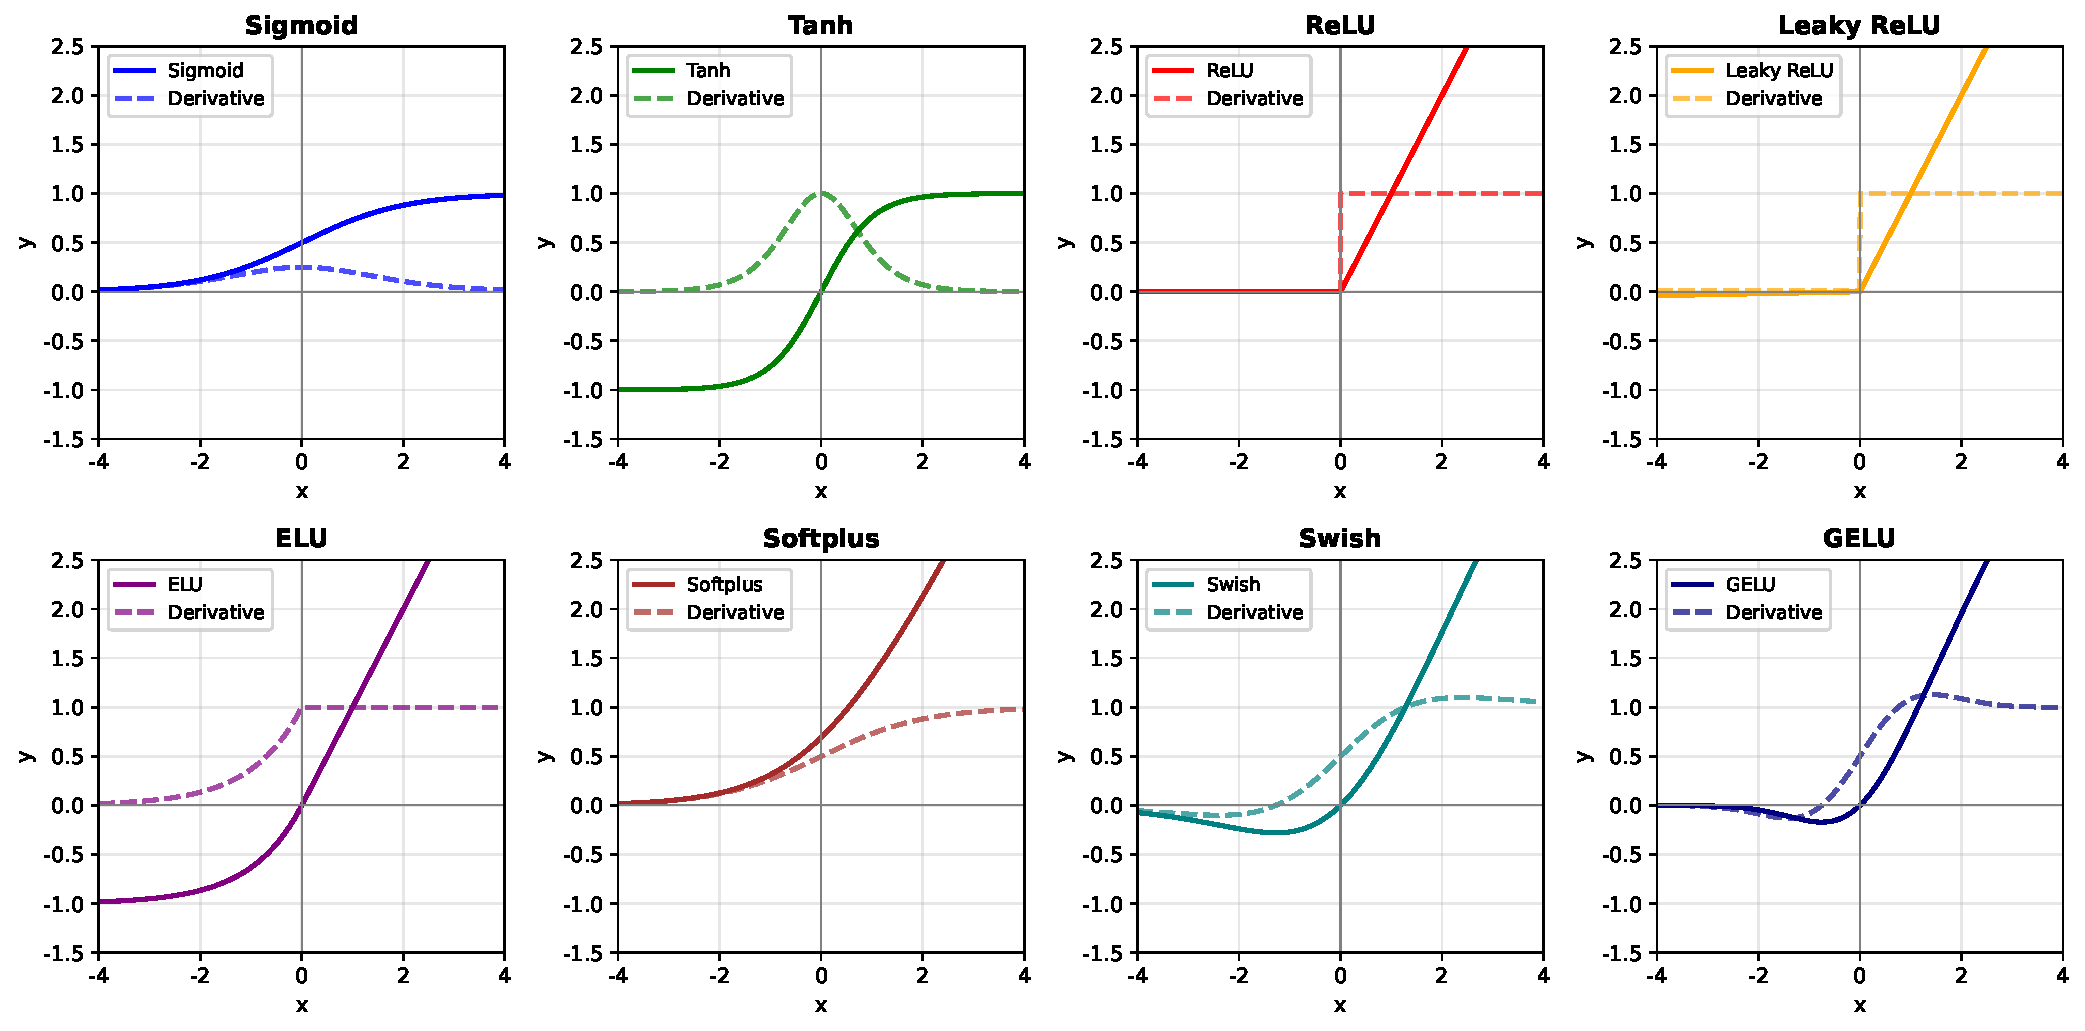
\includegraphics[width=0.95\textwidth]{figs_chap09/activation_functions.pdf}
\caption{常用激活函数（实线）及其导数（虚线）。Sigmoid和Tanh在输入绝对值较大时趋于饱和，导数接近0。ReLU在负半轴完全为0，正半轴导数恒为1。Leaky ReLU、ELU、Swish、GELU都是对ReLU的改进。}
\label{fig:activation_functions}
\end{figure}

\begin{itemize}
    \item \textbf{Sigmoid和Tanh}：输出被"压缩"到有限区间（$[0,1]$或$[-1,1]$），这曾被认为符合生物神经元的激活特性。但它们有严重的\textbf{梯度饱和}问题。

    \item \textbf{ReLU}：极其简单——保留正值，置零负值。计算快、不饱和（正半轴），但可能导致"神经元死亡"。

    \item \textbf{改进版ReLU}：Leaky ReLU、ELU在负半轴保留非零梯度；Swish和GELU则是光滑版本，避免了导数的不连续性。
\end{itemize}

\subsection*{二、手写实现：以Sigmoid为例}

Sigmoid函数的实现看似简单，但有数值陷阱：

\begin{lstlisting}[language=Python]
import numpy as np

def sigmoid_naive(x):
    """朴素实现——可能溢出！"""
    return 1 / (1 + np.exp(-x))

def sigmoid_stable(x):
    """数值稳定实现"""
    return np.where(x >= 0,
                    1 / (1 + np.exp(-x)),
                    np.exp(x) / (1 + np.exp(x)))
\end{lstlisting}

当$x$是很大的负数（如$x = -1000$）时，\texttt{np.exp(-x)}会溢出。稳定版本通过分情况处理避免了这个问题。

Sigmoid的导数有一个优雅的形式：
\[
\sigma'(x) = \sigma(x)(1 - \sigma(x))
\]
这意味着我们可以复用前向传播的结果来计算梯度——这正是深度学习框架的做法。

\subsection*{三、梯度消失问题}

为什么Sigmoid在深度网络中表现不佳？看图\ref{fig:gradient_flow}的中图：

\begin{figure}[htbp]
\centering
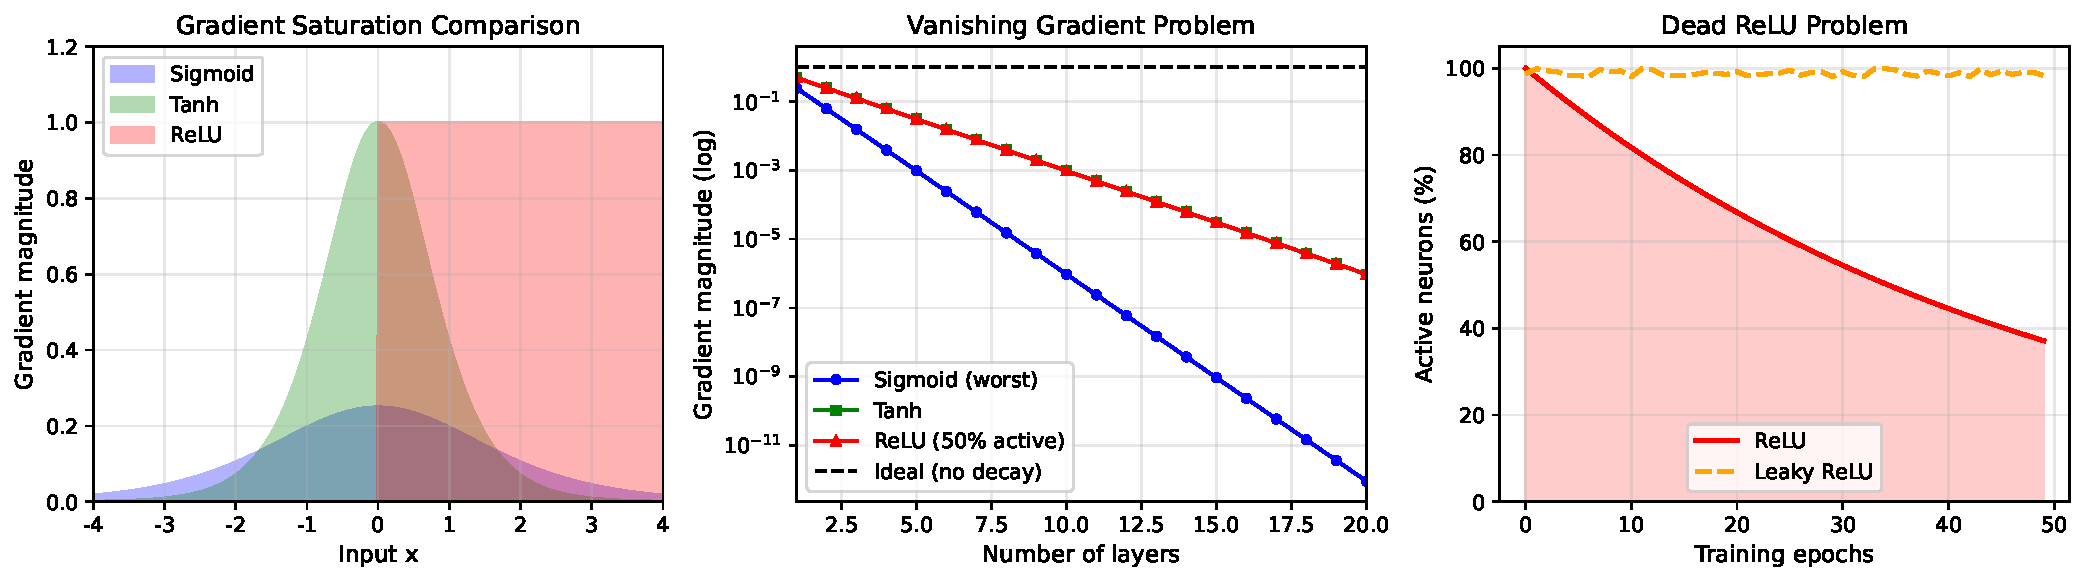
\includegraphics[width=0.95\textwidth]{figs_chap09/gradient_flow.pdf}
\caption{梯度流动分析。左图：不同激活函数的梯度分布。中图：梯度经过多层的衰减（对数尺度）。右图：ReLU的"死亡神经元"问题。}
\label{fig:gradient_flow}
\end{figure}

Sigmoid的最大梯度只有0.25（在$x=0$处）。经过$n$层网络后，梯度最多变成原来的$0.25^n$倍。这就是\textbf{梯度消失}（vanishing gradient）问题——深层网络的参数几乎无法更新。

\marginnote{\textbf{历史注记}：梯度消失问题是神经网络在1990年代陷入低谷的重要原因。直到2006年Hinton等人提出逐层预训练，以及后来ReLU的流行，深度学习才迎来复兴。}

ReLU的优势在于：正半轴的梯度恒为1，不会衰减。这使得梯度可以"无损"地流过任意多层。但ReLU也有代价：负输入的梯度为0，一旦某个神经元进入"死亡"状态，它将永远无法恢复。

\subsection*{四、计算图与反向传播}

理解反向传播的关键是画出\textbf{计算图}（图\ref{fig:computation_graph}）：

\begin{figure}[htbp]
\centering
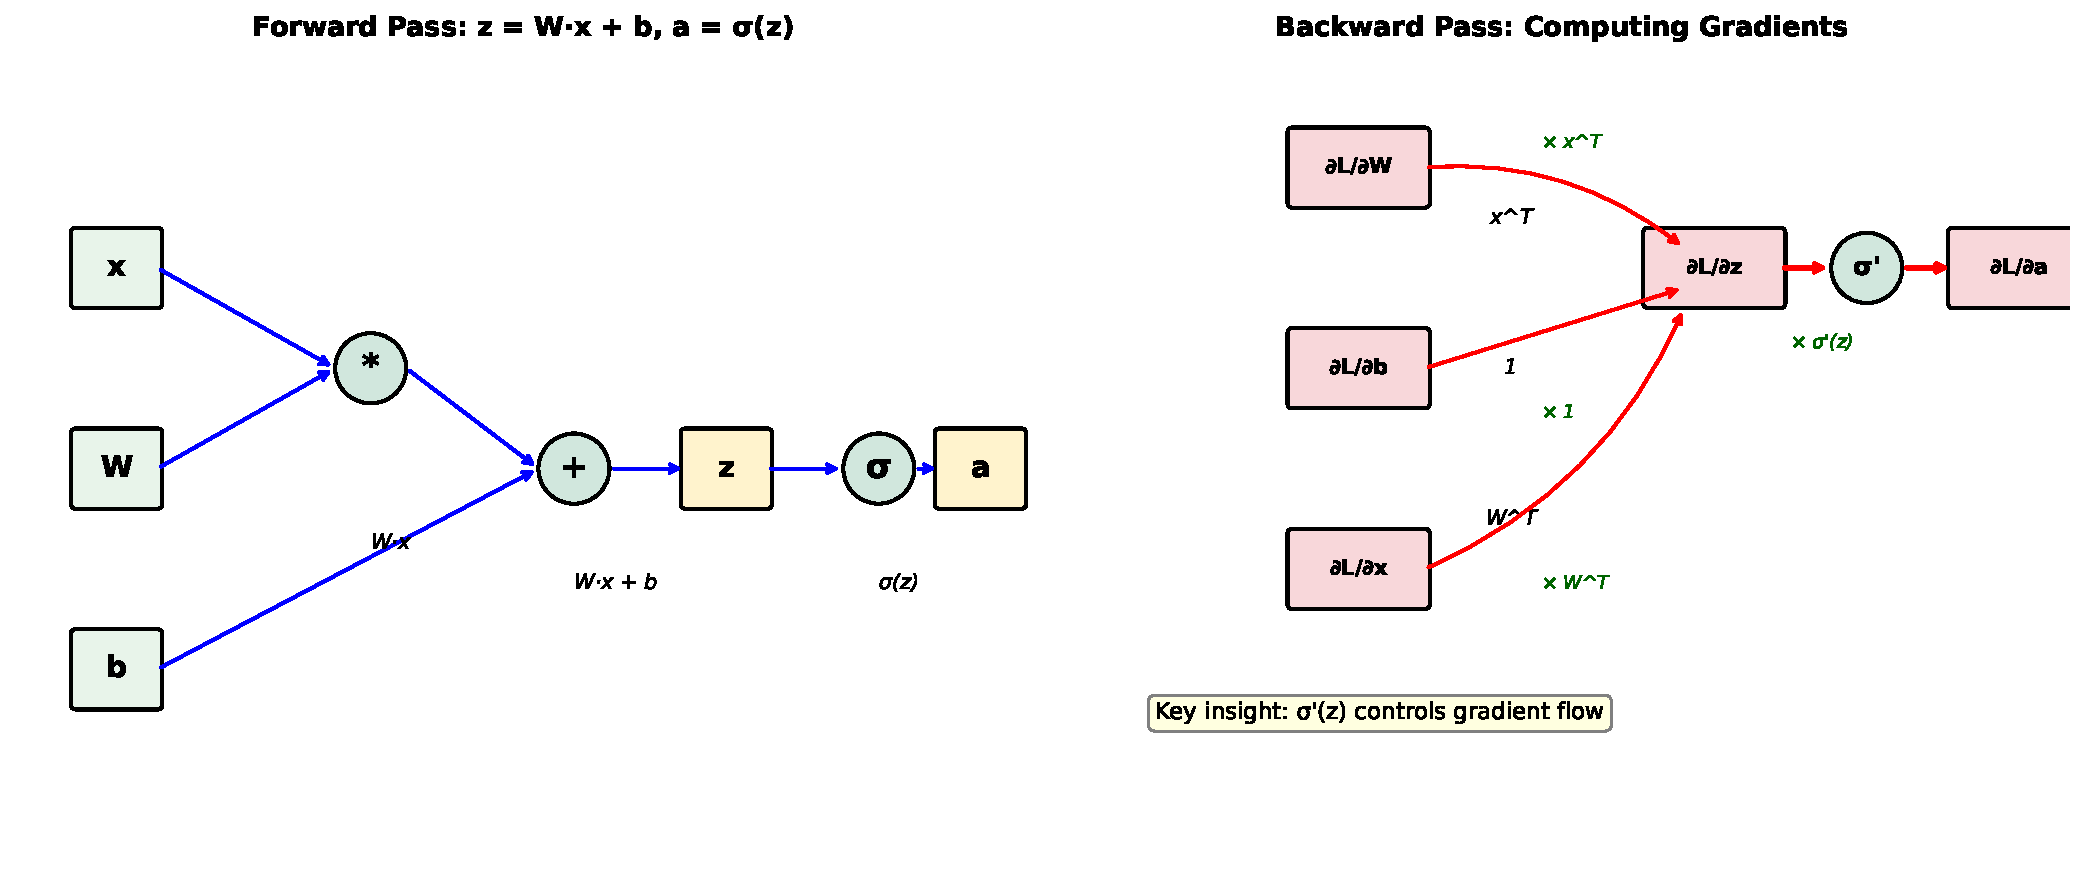
\includegraphics[width=0.95\textwidth]{figs_chap09/computation_graph.pdf}
\caption{单层神经元的计算图。左图：前向传播，从输入$x$计算输出$a$。右图：反向传播，从损失对输出的梯度$\partial L/\partial a$逐步计算对参数$W, b$的梯度。注意$\sigma'(z)$是"阀门"，控制梯度能否有效流回。}
\label{fig:computation_graph}
\end{figure}

前向传播中，信息从左到右流动：$x \to z = Wx+b \to a = \sigma(z)$。

反向传播中，梯度从右到左流动。关键公式是\textbf{链式法则}：
\[
\frac{\partial L}{\partial W} = \frac{\partial L}{\partial a} \cdot \frac{\partial a}{\partial z} \cdot \frac{\partial z}{\partial W} = \frac{\partial L}{\partial a} \cdot \sigma'(z) \cdot x^T
\]

这里$\sigma'(z)$扮演着"阀门"的角色：如果它很小，梯度就流不过去。这解释了为什么激活函数的选择如此重要。

\subsection*{五、梯度检验：验证你的实现}

如何确保手写的梯度公式正确？使用\textbf{数值梯度}验证：
\[
\frac{\partial f}{\partial x} \approx \frac{f(x + \epsilon) - f(x - \epsilon)}{2\epsilon}
\]

图\ref{fig:gradient_check}展示了解析梯度与数值梯度的对比：

\begin{figure}[htbp]
\centering
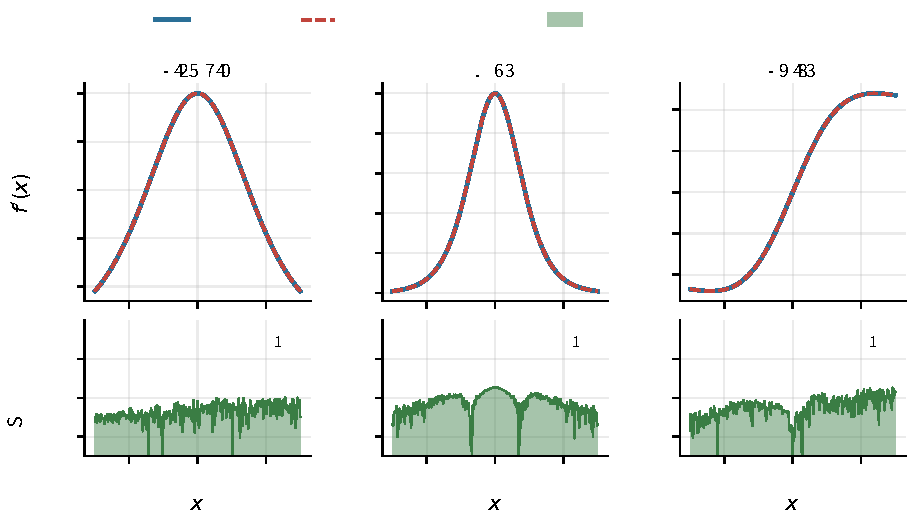
\includegraphics[width=0.95\textwidth]{figs_chap09/gradient_check.pdf}
\caption{梯度检验：解析梯度（蓝色实线）与数值梯度（红色虚线）几乎完全重合。绿色区域显示误差，最大约为$10^{-10}$量级，验证了实现的正确性。}
\label{fig:gradient_check}
\end{figure}

\begin{lstlisting}[language=Python]
def gradient_check(func, deriv, x, eps=1e-5):
    """梯度检验"""
    analytical = deriv(x)
    numerical = (func(x + eps) - func(x - eps)) / (2 * eps)
    error = np.abs(analytical - numerical)
    return error
\end{lstlisting}

如果误差超过$10^{-5}$，很可能你的解析梯度有bug。

\subsection*{六、现代激活函数：GELU与Swish}

GPT和BERT等大模型为什么选择GELU（Gaussian Error Linear Unit）？

\begin{figure}[htbp]
\centering
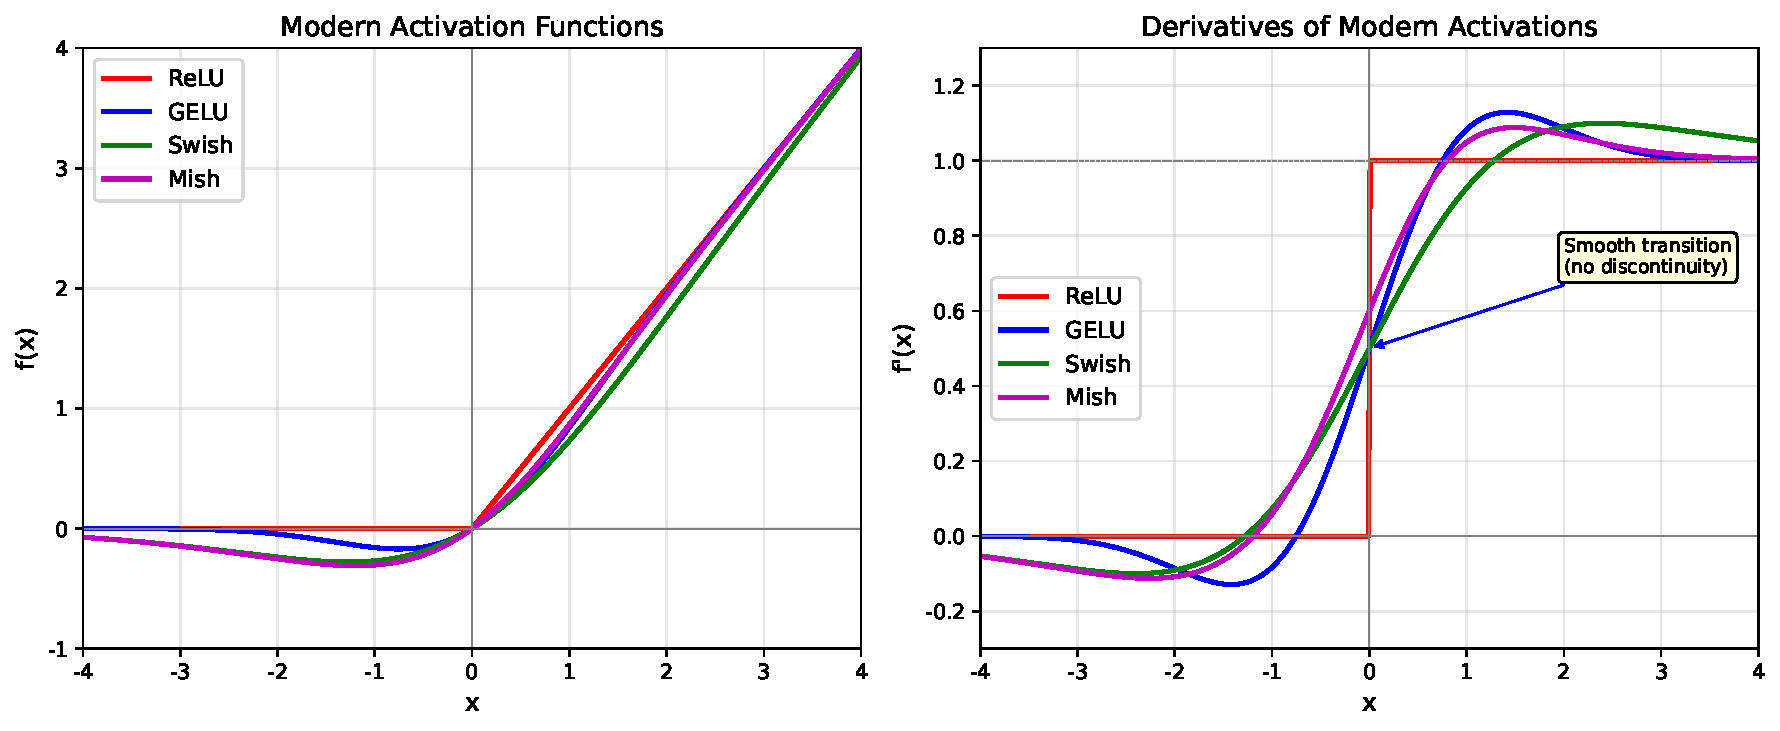
\includegraphics[width=0.9\textwidth]{figs_chap09/modern_activations.pdf}
\caption{现代激活函数对比。GELU、Swish、Mish都是ReLU的光滑近似，在$x=0$附近没有导数的跳跃。右图显示它们的导数曲线，比ReLU更加平滑。}
\label{fig:modern_activations}
\end{figure}

GELU的定义：
\[
\text{GELU}(x) = x \cdot \Phi(x) \approx 0.5x\left(1 + \tanh\left[\sqrt{\frac{2}{\pi}}\left(x + 0.044715x^3\right)\right]\right)
\]
其中$\Phi(x)$是标准正态分布的CDF。

直觉：GELU对输入$x$进行"随机门控"——输入越大，通过的概率越高。这可以看作对dropout的可微近似。

Swish则更简单：$\text{Swish}(x) = x \cdot \sigma(x)$。

这些光滑激活函数的优势：
\begin{itemize}
    \item 导数处处连续，优化过程更稳定
    \item 负半轴不完全为0，避免神经元死亡
    \item 在大规模模型上的实验效果略优于ReLU
\end{itemize}

\subsection*{七、手写自动微分}

最后，我们展示如何用50行代码实现支持激活函数的自动微分：

\begin{lstlisting}[language=Python]
class Tensor:
    def __init__(self, data):
        self.data = data
        self.grad = 0
        self._backward = lambda: None
        self._prev = set()

    def sigmoid(self):
        s = 1 / (1 + np.exp(-self.data))
        out = Tensor(s)
        out._prev = {self}
        def _backward():
            self.grad += s * (1 - s) * out.grad  # 链式法则！
        out._backward = _backward
        return out

    def backward(self):
        # 拓扑排序
        topo = []
        visited = set()
        def build_topo(v):
            if v not in visited:
                visited.add(v)
                for child in v._prev:
                    build_topo(child)
                topo.append(v)
        build_topo(self)

        # 反向传播
        self.grad = 1
        for v in reversed(topo):
            v._backward()
\end{lstlisting}

核心思想：每个操作（如Sigmoid）都记录"如何把输出的梯度传递给输入"。反向传播时，按拓扑逆序依次调用这些函数。

完整代码见\texttt{code\_chap09/activation\_functions.py}。

\subsection*{八、设计哲学小结}

激活函数的演化体现了深度学习的工程智慧：

\begin{enumerate}
    \item \textbf{生物启发 → 数学便利}：Sigmoid模拟神经元激活概率，但数学性质不好。ReLU虽不生物，但训练效果好。

    \item \textbf{简单 → 光滑}：ReLU计算快但不连续，GELU光滑但计算稍贵。在大模型时代，光滑性带来的稳定性更重要。

    \item \textbf{理论 → 实验}：没有任何理论证明GELU一定比ReLU好。选择激活函数更多靠实验调参。
\end{enumerate}

\begin{insightbox}[title=实践建议]
\begin{itemize}
    \item \textbf{默认选ReLU}：简单、快、效果好
    \item \textbf{大模型用GELU}：GPT/BERT的标配
    \item \textbf{遇到"死神经元"换Leaky ReLU}：负半轴保留梯度
    \item \textbf{不确定就实验}：在你的任务上跑几个对比
\end{itemize}
\end{insightbox}

%======================================================================
\section*{扩展阅读：为什么不能随便选择神经网络架构}
\addcontentsline{toc}{section}{扩展阅读：神经网络架构选择}
%======================================================================

神经网络通常被写成一个参数化函数
\[
f_\theta : \mathcal{X} \to \mathcal{Y},
\]
其中 $\theta$ 是网络的所有参数（权重与偏置）。给定一个输入 $x\in\mathcal{X}$，网络输出 $f_\theta(x)$ 作为预测或表示。

不同的网络结构，对 $f_\theta$ 所在的函数集合施加了不同的约束：
\[
\mathcal{F}_{\text{MLP}} \neq \mathcal{F}_{\text{CNN}} \neq \mathcal{F}_{\text{RNN}} \neq \mathcal{F}_{\text{Transformer}} \neq \mathcal{F}_{\text{GNN}}.
\]
这里的 $\mathcal{F}$ 可以理解为"在有限参数规模与有限深度下，网络实际能够高效表示的函数类"。

虽然多层感知机（MLP）在理论上具有通用逼近能力，可以逼近任意连续函数，但在有限宽度、有限深度和有限训练样本的条件下，不同结构对不同类型数据的表达效率差异巨大。本节从公式与直觉两方面，分析典型网络结构与数据结构之间的对应关系，并给出一些"某一结构难以识别、另一结构容易识别"的具体例子。

%----------------------------------------------------------------------
\subsection*{一、基本单元：仿射变换与非线性}
%----------------------------------------------------------------------

\paragraph{单个神经元的计算形式}

最基本的神经元对输入向量 $x\in\mathbb{R}^d$ 的计算为
\[
y = \sigma(w^\top x + b),
\]
其中 $w\in\mathbb{R}^d$ 为权重向量，$b\in\mathbb{R}$ 为偏置，$\sigma(\cdot)$ 为非线性激活函数（如 ReLU, Sigmoid 等）。

几何意义上，$w^\top x + b = 0$ 表示 $\mathbb{R}^d$ 中的一个超平面。对于二分类任务，若将输出二值化：
\[
\hat{y} = \begin{cases} 1, & \sigma(w^\top x + b) \ge \tau,\\ 0, & \text{否则}, \end{cases}
\]
该神经元实质上实现了一个线性分类器，决策边界是一个超平面。

\paragraph{单隐层前馈网络}

一个含单隐层，宽度为 $m$ 的前馈神经网络可以写成
\[
f(x) = \sum_{i=1}^m \alpha_i \,\sigma(w_i^\top x + b_i) + c,
\]
其中 $w_i, b_i$ 为第 $i$ 个隐层神经元的参数，$\alpha_i, c$ 为输出层的参数。

此类网络在理论上满足通用逼近定理：当 $m\to\infty$ 时，在 mild 条件下可以逼近任意连续函数。然而，在固定宽度 $m$ 下，能方便表示的函数仍有强烈结构性。不同的网络结构可以被视为在以下几个方面作出不同的"工程性假设"：

\begin{itemize}
\item 输入特征之间是否存在空间或拓扑结构；
\item 函数是否具有平移、旋转或其他对称性；
\item 是否存在时间或序列依赖；
\item 是否存在图结构（节点与边）约束。
\end{itemize}

后续各节将围绕这些问题展开。

%----------------------------------------------------------------------
\subsection*{二、线性可分性与 XOR：一层网络的能力极限}
%----------------------------------------------------------------------

\paragraph{线性可分与决策边界}

考虑二分类问题，输入 $x\in\mathbb{R}^2$，输出 $y\in\{0,1\}$。若存在某个 $(w,b)$ 使得
\[
w^\top x + b > 0 \Rightarrow y=1,\quad w^\top x + b < 0 \Rightarrow y=0,
\]
则称该数据集合 \emph{线性可分}。此时仅用一个神经元即可实现完美分类，决策边界是平面（在二维即直线）。

若数据不是线性可分，则单个神经元无论如何调整 $w,b$ 都不可能实现零训练误差。这种情况需要多个神经元组合，利用非线性叠加构造更复杂的边界。

\paragraph{XOR 示例：典型的非线性可分问题}

考虑逻辑异或运算 XOR：
\[
\text{XOR}(x_1,x_2) = \begin{cases} 1, & x_1 \ne x_2,\\ 0, & x_1 = x_2. \end{cases}
\]
对应的四个输入--输出对为：
\[
(0,0)\to 0,\quad (1,1)\to 0,\quad (1,0)\to 1,\quad (0,1)\to 1.
\]

将这些点画在二维平面上，可以观察到：

\begin{itemize}
\item $(0,0)$ 与 $(1,1)$ 属于一类；
\item $(1,0)$ 与 $(0,1)$ 属于另一类；
\item 无论怎样画一条直线，都无法将这两类点完全分开。
\end{itemize}

因此 XOR 数据不是线性可分的。一层感知机的决策边界为 $w_1x_1 + w_2x_2 + b = 0$，只能得到一条直线，即只能表示线性可分类。故一层网络无法表示 XOR 函数。

\paragraph{两层网络如何表示 XOR}

引入一个含两个隐含神经元的网络：
\[
h_1 = \sigma(w_1^\top x + b_1), \quad h_2 = \sigma(w_2^\top x + b_2), \quad f(x) = \sigma(\alpha_1 h_1 + \alpha_2 h_2 + c).
\]

可以构造如下形式（用 Heaviside 函数 $H$ 直观说明）：
\[
h_1 = H(x_1 - x_2),\quad h_2 = H(x_2 - x_1).
\]
此时
\[
h_1 = \begin{cases} 1, & x_1 > x_2,\\ 0, & \text{否则}, \end{cases} \quad h_2 = \begin{cases} 1, & x_2 > x_1,\\ 0, & \text{否则}. \end{cases}
\]
对 XOR 的四个点：
\[
\begin{aligned}
(0,0): &\quad h_1=0,\ h_2=0,\\
(1,1): &\quad h_1=0,\ h_2=0,\\
(1,0): &\quad h_1=1,\ h_2=0,\\
(0,1): &\quad h_1=0,\ h_2=1.
\end{aligned}
\]
可以令输出层为
\[
f(x) = H(h_1 + h_2 - 0.5),
\]
则恰好得到 XOR。这里两层结构将平面划分为多个线性区域，再通过线性组合与非线性得到非线性决策边界。

这个例子说明：即使有非线性激活，一层结构的表达能力仍严格受限，只能表示线性可分问题。增加一层后，决策边界可以组合多个线性片段，从而表示更复杂模式。

%----------------------------------------------------------------------
\subsection*{三、卷积网络与局部结构：为什么 CNN 在图像上高效}
%----------------------------------------------------------------------

\paragraph{图像的局部相关性与平移等变性}

将灰度图像视为矩阵 $X \in \mathbb{R}^{H\times W}$，每个像素 $X_{i,j}$ 与其邻近像素在空间上高度相关。许多模式（边缘、角点、纹理）具有以下特征：

\begin{itemize}
\item \textbf{局部性}：可以仅通过一个小邻域（例如 $3\times 3$）来判断；
\item \textbf{平移等变性}：同一个局部模式出现在图像的不同位置时，其语义一致。
\end{itemize}

将这两点作为假设，可以构造卷积神经网络。

\paragraph{卷积运算的形式}

以二维卷积为例，给定卷积核 $K\in\mathbb{R}^{k\times k}$，卷积运算为
\[
(Y = K * X)_{i,j} = \sum_{u=-r}^r \sum_{v=-r}^r K_{u,v}\, X_{i+u, j+v},
\]
其中 $k = 2r+1$。该公式反映两点重要性质：

\begin{itemize}
\item \textbf{局部感受野}：输出 $Y_{i,j}$ 只依赖于输入中 $(i,j)$ 附近的像素；
\item \textbf{权重共享}：同一个卷积核 $K$ 在整张图像上平移使用。
\end{itemize}

若将图像展开为向量 $x\in\mathbb{R}^{HW}$，则卷积对应一个稀疏矩阵 $W_{\text{conv}}$：
\[
\text{vec}(Y) = W_{\text{conv}}\, \text{vec}(X),
\]
其中 $W_{\text{conv}}$ 的非零结构体现了局部连接和权重共享。

与之对比，如果使用全连接层：
\[
y = W_{\text{fc}}\, \text{vec}(X) + b,
\]
矩阵 $W_{\text{fc}}$ 为稠密矩阵，需要 $O(H^2 W^2)$ 个参数，既不利用局部性，也不利用平移不变性；卷积核则只需 $k^2$ 个参数。

\paragraph{边缘检测示例：卷积核的优势}

考虑一幅 $5\times 5$ 的简化图像，包含一条水平边缘：
\[
X = \begin{bmatrix} 1 & 1 & 1 & 1 & 1\\ 1 & 1 & 1 & 1 & 1\\ 0 & 0 & 0 & 0 & 0\\ 0 & 0 & 0 & 0 & 0\\ 0 & 0 & 0 & 0 & 0 \end{bmatrix}.
\]

定义一个垂直边缘检测的卷积核（Sobel 样式）：
\[
K = \begin{bmatrix} 1 & 0 & -1\\ 1 & 0 & -1\\ 1 & 0 & -1 \end{bmatrix}.
\]

对 $X$ 做卷积，局部窗口中亮度差显著处（即边缘）会产生较大响应。卷积核不需要知道边缘出现在图像哪里，只要局部模式相同，响应便相同，这体现了平移等变性。

若用全连接层来手动"学习"边缘检测，则需要为每个可能的边缘位置学习一组单独参数，参数量极大，并且难以泛化到未见过的位置。卷积核通过共享参数，在整个图像上复用同一模式检测器。

\paragraph{从函数类角度的对比}

全连接网络可以表示的线性映射集合为所有 $HW \times HW$ 的矩阵；卷积网络可以表示的线性映射集合仅是其中满足"Toeplitz 块结构"的一小部分。形式上：
\[
\mathcal{L}_{\text{conv}} \subset \mathcal{L}_{\text{fc}}.
\]

这一"缩小函数空间"的操作相当于引入明显且符合图像物理结构的归纳偏置，使得在相同参数规模下，卷积网络在图像任务上能够更高效地拟合正确映射。

%----------------------------------------------------------------------
\subsection*{四、序列建模：RNN 与 Transformer 对长依赖的处理}
\preview{第11章会专门推导 RNN 的梯度消失（把本章的伴随方程沿时间展开）并介绍 Transformer 的注意力机制；这里只从"函数类"的角度做个预告。}
%----------------------------------------------------------------------

\paragraph{RNN 的递推结构}

给定一个长度为 $T$ 的序列 $(x_1, x_2, \dots, x_T)$，循环神经网络（RNN）定义隐状态递推为：
\[
h_t = \phi(W_h h_{t-1} + W_x x_t + b),
\]
输出为
\[
y_t = \psi(W_y h_t + c).
\]

这里 $h_t$ 可以视为对前 $t$ 个输入的"压缩记忆"。理论上，$h_t$ 包含所有历史信息：
\[
h_t = F(x_1, x_2, \dots, x_t).
\]

然而在实践中，由于链式乘积的存在，参数学习会面临梯度消失或爆炸问题。

\paragraph{梯度消失的简要分析}

以损失 $L$ 对某一时刻状态 $h_t$ 的梯度为例：
\[
\frac{\partial L}{\partial h_t} = \frac{\partial L}{\partial h_T} \prod_{k=t+1}^{T} \frac{\partial h_k}{\partial h_{k-1}}.
\]
若将 $\frac{\partial h_k}{\partial h_{k-1}}$ 近似写作某个矩阵 $J_k$，则
\[
\left|\frac{\partial L}{\partial h_t}\right| \le \left|\frac{\partial L}{\partial h_T}\right| \cdot \prod_{k=t+1}^{T} \|J_k\|.
\]
如果 $\|J_k\| < 1$，则该乘积随着 $T-t$ 增大会快速趋向 0，造成梯度消失，从而较难捕获长距离依赖；若 $\|J_k\| > 1$，则会出现梯度爆炸。

LSTM、GRU 等结构通过门控机制缓解这一问题，但根本上仍基于顺序递推。

\paragraph{长依赖示例：远距离一致性}

考虑一个简化任务：输入为括号序列，如
\[
\texttt{( ( ) ( ( ) ) )},
\]
任务是判断括号是否匹配。判断最后一个右括号是否匹配，需要考虑整个序列的结构信息。

RNN 需要在 $h_t$ 中长期保存栈式信息，且训练时梯度需要通过长链传播，容易出现训练困难。在理论上，足够大的 RNN 可以模拟栈机，但在有限参数和梯度下降的训练机制下，学习到稳定的栈行为非常困难。

\paragraph{Transformer 的自注意力机制}

Transformer 使用自注意力机制（self-attention）直接让每个位置与全序列交互。对长度为 $T$ 的序列，先通过线性变换得到
\[
Q = X W_Q,\quad K = X W_K,\quad V = X W_V,
\]
其中 $X\in\mathbb{R}^{T\times d}$ 为输入序列表示，$Q,K,V\in\mathbb{R}^{T\times d_k}$。

自注意力输出为
\[
\text{Attn}(Q,K,V) = \text{softmax}\left(\frac{QK^\top}{\sqrt{d_k}}\right)V.
\]

其中 $(QK^\top)_{ij} = q_i^\top k_j$ 表示位置 $i$ 对位置 $j$ 的相关性。对于每个位置 $i$：
\[
\tilde{h}_i = \sum_{j=1}^{T} \alpha_{ij} v_j,\quad \alpha_{ij} = \frac{\exp(q_i^\top k_j / \sqrt{d_k})}{\sum_{l=1}^{T} \exp(q_i^\top k_l / \sqrt{d_k})}.
\]

这种结构的关键特点是：\emph{任意两个位置之间可以通过单层注意力直接建立联系}，不需要经过多步递推。对于前面的括号任务，某个位置可以直接"关注"与之匹配的括号位置，因此在函数表达上更适合建模远距离依赖。

\paragraph{从函数表达角度的对比}

RNN 所表达的函数类通过递推定义：
\[
h_t = F(h_{t-1}, x_t),
\]
而 Transformer 的自注意力层本质上表达了"任意位置两两交互"的函数：
\[
\tilde{h}_i = G\left(\{x_j\}_{j=1}^{T}\right),
\]
且 $G$ 在构造上具有对位置重排的某些对称性（通过位置编码调节）。从函数空间角度看，Transformer 引入的自注意力操作扩展了对非局部依赖的直接表达能力，使得在有限深度下更容易表示需要远距离交互的函数。

%----------------------------------------------------------------------
\subsection*{五、图结构数据与图神经网络}
%----------------------------------------------------------------------

\paragraph{图结构数据的特征}

图 $G = (V, E)$ 由节点集合 $V$ 与边集合 $E$ 组成。典型例子包括：

\begin{itemize}
\item 社交网络：节点为用户，边为好友关系；
\item 交通网络：节点为路口或站点，边为道路或轨道；
\item 电力网络：节点为变电站或母线，边为输电线路；
\item 分子结构：节点为原子，边为化学键。
\end{itemize}

图数据的重要特征在于：拓扑结构本身承载了关键信息。节点的功能不仅由其自身特征决定，还由其邻居及更远节点的结构关系决定。

\paragraph{图神经网络的消息传递框架}

图神经网络（Graph Neural Network, GNN）的一个典型形式是消息传递神经网络（Message Passing Neural Network, MPNN）。在第 $k$ 层，第 $i$ 个节点特征更新规则为：
\[
h_i^{(k+1)} = \phi\Big(h_i^{(k)},\ \square_{j\in\mathcal{N}(i)} \psi\big(h_i^{(k)}, h_j^{(k)}, e_{ij}\big)\Big),
\]
其中
\begin{itemize}
\item $h_i^{(k)}$ 为节点 $i$ 在第 $k$ 层的表示；
\item $\mathcal{N}(i)$ 为节点 $i$ 的邻居集合；
\item $e_{ij}$ 为边 $(i,j)$ 的特征；
\item $\psi$ 为消息函数，$\phi$ 为更新函数；
\item $\square$ 为一个置换不变的聚合算子（如求和、平均或最大）。
\end{itemize}

该形式体现了图结构的两个关键性质：

\begin{itemize}
\item \textbf{局部性}：节点表示由邻居的表示聚合而来；
\item \textbf{置换不变性}：邻居节点顺序可以任意变换，不影响聚合结果。
\end{itemize}

\paragraph{图结构上 CNN 的局限}

若尝试将普通 CNN 直接应用于图，存在若干困难：

\begin{itemize}
\item 图通常是非规则结构，不存在自然的二维网格坐标 $(i,j)$；
\item 不同节点的度数不同，难以定义固定形状的"卷积核邻域"；
\item 图结构不存在平移对称性，不能简单依赖权重共享在规则网格上的平移。
\end{itemize}

因此，传统卷积无法直接刻画图上的邻接关系与拓扑属性。而 GNN 通过邻居聚合的形式，将图的邻接结构内置到更新规则中。例如，一阶 GCN（Graph Convolutional Network）层可写作：
\[
H^{(k+1)} = \sigma\left(\tilde{D}^{-1/2} \tilde{A} \tilde{D}^{-1/2} H^{(k)} W^{(k)}\right),
\]
其中 $\tilde{A} = A + I$ 为加入自环的邻接矩阵，$\tilde{D}$ 为对应度矩阵，$H^{(k)}$ 为所有节点的表示矩阵。该结构利用了图拉普拉斯算子的谱特性，从谱图论角度实现了"图上的卷积"。

\paragraph{拓扑敏感任务中的结构差异}

考虑以下任务：给定电力网络拓扑与各节点负荷，预测某条线路是否存在过载风险。该任务的输出不仅取决于某条线的局部属性，还取决于整个网络的潮流分布。

若将网络拓扑展开为某种顺序向量输入全连接网络，理论上可以表达正确函数，但需要网络在训练中"重新学会"图的拓扑结构与 Kirchhoff 定律之类的物理约束，学习效率低。而 GNN 在结构上即按照图拓扑传播与聚合信息，更接近实际物理过程，因此在相同参数规模下更容易学习到合理函数。

%----------------------------------------------------------------------
\subsection*{六、函数空间与归纳偏置}
%----------------------------------------------------------------------

\paragraph{通用逼近与有效逼近}

多层感知机的通用逼近定理表明：对于紧致集合上的任意连续函数 $f$，存在一个宽度足够的大单隐层网络，使得
\[
\sup_{x\in K} |f(x) - f_\theta(x)| < \varepsilon
\]
对任意 $\varepsilon>0$ 成立。

然而该定理没有给出网络宽度、参数规模与逼近误差之间的有效关系，也没有考虑训练算法与数据分布。实际中更关心的问题是：在给定参数预算与数据规模下，哪类结构能够"高效"表示目标函数。

\paragraph{结构约束下的函数类}

可以将不同结构的网络理解为在参数空间 $\Theta$ 上施加不同的结构约束，从而改变可表达函数集：
\[
\mathcal{F} = \{f_\theta : \theta\in\Theta\}.
\]

\begin{itemize}
\item 对于全连接网络，$\Theta_{\text{fc}}$ 包含所有稠密矩阵参数，$\mathcal{F}_{\text{fc}}$ 十分宽泛；
\item 对于卷积网络，$\Theta_{\text{conv}}$ 仅包含卷积核参数，且强制权重共享，$\mathcal{F}_{\text{conv}}$ 是 $\mathcal{F}_{\text{fc}}$ 的一个子集；
\item 对于 RNN/Transformer/GNN，$\Theta$ 中都包含特定形式的权重共享、对称性或拓扑约束。
\end{itemize}

这些约束可以被视为归纳偏置（inductive bias）：在函数空间中优先选择满足某些不变性或等变性的函数。例如：

\begin{itemize}
\item 卷积层偏向选择平移等变函数；
\item GNN 偏向选择在节点重标号下保持不变的图函数；
\item 自注意力层偏向选择依赖于 token 间相对相似性的函数。
\end{itemize}

\paragraph{对称性与等变性}

设有一组变换构成的群 $G$（例如图像的平移群）。若函数 $f$ 满足
\[
f(T_g x) = f(x),\quad \forall g\in G,
\]
称 $f$ 对 $G$ 不变；若满足
\[
f(T_g x) = T'_g f(x),
\]
称 $f$ 对 $G$ 等变。卷积网络通过局部感受野与权重共享，实现了对平移的等变性；池化操作进一步导致对平移的不变性。

\paragraph{归纳偏置与数据结构匹配}

当数据的真实生成机制具有某种对称性或结构时，将相同的结构内置到网络中，可以显著减少所需参数与训练样本。相反，若选择与数据结构不匹配的网络结构，则需要更多参数、更多数据才能"在函数空间中搜索到"合适的函数，甚至在有限资源下根本难以学到。

从这个角度看，不同架构的"适用领域"可以概括为：

\begin{itemize}
\item MLP：适合无明显空间或拓扑结构的小规模特征；
\item CNN：适合具有局部相关性和平移等变性的网格数据（图像、某些 PDE 网格）；
\item RNN/LSTM：适合中短距离依赖为主的序列；
\item Transformer：适合存在长距离依赖或全局交互的序列与多模态数据；
\item GNN：适合拓扑结构重要、以图为基本对象的数据。
\end{itemize}

%----------------------------------------------------------------------
\subsection*{七、小结}
%----------------------------------------------------------------------

本节从公式与结构出发，讨论了不同神经网络架构与不同类型问题之间的对应关系。主要结论可以概括如下：

\begin{enumerate}
\item 单层网络（线性分类器）只能实现线性可分问题，典型反例是 XOR；增加层数后，通过叠加多个仿射变换与非线性，可以构造更复杂的分段线性决策边界。

\item 卷积网络通过局部感受野与权重共享假设，内置了对平移等变性的归纳偏置，极大提高了在图像等网格结构数据上的表达效率；全连接网络虽然理论上也能表示相同函数，但参数规模与学习难度远大于卷积网络。

\item RNN 通过递推关系建模序列，但梯度需要沿时间方向传播，容易出现梯度消失，难以捕获长距离依赖；Transformer 的自注意力机制允许任意位置之间直接交互，在表达远距离依赖方面更具优势。

\item 图神经网络通过消息传递与邻居聚合机制，将图的拓扑结构直接编码到网络更新规则中，适合处理社交网络、电网、交通网络等图结构数据；传统 CNN 由于依赖规则网格和平移对称性，难以直接应用于一般图。

\item 从函数空间与归纳偏置的角度看，不同架构对应不同的可表达函数类。通过引入与数据生成机制相匹配的结构性假设，可以在有限参数和样本条件下，更高效地学习到合理的函数映射。
\end{enumerate}

在具体应用中，网络结构的选择可以被理解为：对数据结构、任务需求与物理或统计规律的一种工程化编码。理解这些结构背后的数学与直观假设，是构建有效深度学习模型的重要基础。  % 第9章：深度学习与反向传播
% ====================================================================================
\chapter{强化学习：从约束优化到智能决策}
% ====================================================================================


\marginnote{\textbf{理查德·贝尔曼}(1920--1984)：美国应用数学家，动态规划之父。他在兰德公司工作期间创立了这一领域，后获IEEE荣誉奖章。``维数灾难''一词也是他首创的。贝尔曼方程如今是强化学习和最优控制的核心。}

1953年的一个下午，美国数学家理查德·贝尔曼（Richard Bellman）正在兰德公司的办公室里思考一个看似简单的问题：如何做出一系列最优决策？

当时正值冷战，美国国防部需要优化各种军事后勤问题——补给路线、资源分配、作战规划。这些问题有一个共同特点：今天的决策会影响明天的选择，明天的选择又会影响后天......决策像多米诺骨牌一样环环相扣。

贝尔曼发现了一个优美的原理：\textbf{无论你现在处于什么状态，从现在到终点的最优策略，不依赖于你是怎么到达现在这个状态的}。换句话说，"过去的就让它过去吧"——最优决策只需要看当前状态和未来，不需要纠结历史。

贝尔曼后来回忆，他选择"动态规划"（Dynamic Programming）这个名字是为了"听起来很厉害"，好让国防部的官员们批准研究经费。"Programming"在当时指"规划"而非"编程"，而"Dynamic"则是为了避开当时国防部长对"数学研究"的反感。

这个原理被称为\textbf{最优性原理}（Principle of Optimality），由此推导出的方程被命名为\textbf{贝尔曼方程}（Bellman Equation）。七十年后的今天，这个方程正在AlphaGo的棋盘上、ChatGPT的对话中、波士顿动力机器狗的每一步里默默运行。

但贝尔曼方程从何而来？教科书通常把它当作"定义"直接给出。本章将揭示一个更深刻的事实：\textbf{贝尔曼方程是约束优化问题的KKT条件}，而值函数$V(s)$正是我们熟悉的拉格朗日乘子！

\begin{quote}
\textbf{本章目标}：
\begin{enumerate}
    \item 从约束优化的角度推导贝尔曼方程
    \item 通过最短路问题理解"对偶上升"与"原始改进"两种求解思路
    \item 建立对强化学习各种算法的统一认识
\end{enumerate}
\end{quote}

\begin{tcolorbox}[colback=green!5, colframe=green!60!black, title=学完这章，你将能够...]
\begin{itemize}
    \item 把序贯决策问题写成约束优化形式
    \item 推导并求解简单MDP的贝尔曼方程
    \item 实现Value Iteration和Policy Iteration算法
    \item 理解Q-learning、DQN、PPO等算法的核心思想
    \item 分析值函数作为拉格朗日乘子的经济学含义
\end{itemize}
\end{tcolorbox}

% ------------------------------------------------------------------------------------
\section{智能体的决策问题}
% ------------------------------------------------------------------------------------

\subsection{问题描述}

想象你在玩一个游戏。在每个时刻$t$：
\begin{itemize}
    \item 你处于某个\textbf{状态} $s_t$（比如棋盘局面、机器人的位置和速度）
    \item 你选择一个\textbf{动作} $a_t$（比如落子位置、关节力矩）
    \item 环境给你一个\textbf{奖励} $r_t$（比如吃掉对方棋子得分、向目标前进得分）
    \item 环境进入下一个状态 $s_{t+1}$
\end{itemize}

\marginnote{\textbf{有趣的历史}：在强化学习中，动作叫action，记作$a$；而在控制理论中，控制量却几乎总是记作$u(t)$。

原因来自前苏联控制论传统——"控制"在俄语中是«{\cyrillicfont управление}»（u-prav-lé-nie），首字母正是俄文字母«{\cyrillicfont У}»（对应拉丁字母U），因此控制量自然记为$u$。

也就是说，RL的$a$和控制论的$u$来自冷战时期两套独立发展的理论体系，最终在现代机器人学习中再次汇合。}

你的目标是让\textbf{累积奖励最大}：
\begin{equation}
    J = r_0 + \gamma r_1 + \gamma^2 r_2 + \cdots = \sum_{t=0}^{\infty} \gamma^t r_t
\end{equation}

这里$\gamma \in (0,1)$叫做\textbf{折扣因子}。为什么需要它？

\textbf{数学原因}：如果$\gamma = 1$且游戏永远不结束，无穷级数可能发散。$\gamma < 1$保证级数收敛。

\textbf{现实原因}："一鸟在手胜过双鸟在林"——今天的一块钱比明天的一块钱更值钱。$\gamma$正是这种时间偏好的数学表达。

\subsection{关键洞察：动力学是约束}

游戏有规则！你不能随意瞬移到任何状态，必须遵循状态转移方程：
\begin{equation}
    s_{t+1} = f(s_t, a_t)
\end{equation}

停下来想一想：这个方程在说什么？

它说的是：给定当前状态$s_t$和你的动作$a_t$，下一个状态$s_{t+1}$就被\textbf{唯一确定}了。你没有选择的余地——这是物理世界的规则，是你必须遵守的\textbf{约束}。

于是，强化学习问题可以写成我们熟悉的约束优化形式：

\begin{keyformula}[title=强化学习的约束优化形式]
\begin{equation}
    \max_{\{a_t\}_{t=0}^{\infty}} \sum_{t=0}^{\infty} \gamma^t r(s_t, a_t) \quad \text{subject to} \quad s_{t+1} = f(s_t, a_t), \quad \forall t \geq 0
\end{equation}
\end{keyformula}

这和我们在前面章节学过的约束优化问题有着完全相同的结构！唯一的区别是这里有无穷多个时刻，因此有无穷多个约束。
\clarify{对比一下：第3章变分法的约束是$y_{k+1} - y_k = v_k\Delta x$，第4章力学的约束是$\dot{q} = v$，这里的约束是$s_{t+1} = f(s_t, a_t)$。形式完全一样！只是变量名不同：位置/状态/state，速度/动作/action。}

\begin{keyidea}{强化学习问题的输入与输出——给大二同学的说明}
\textbf{你在解决什么问题？}

一个智能体在环境中行动，每一步都会获得奖励。你的目标是找到最优策略，使得累积奖励最大。

\textbf{输入（你需要知道的）}：
\begin{itemize}
    \item \textbf{状态空间}$\mathcal{S}$：智能体可能处于的所有状态（如机器人的位置、速度）
    \item \textbf{动作空间}$\mathcal{A}$：智能体可以采取的所有动作（如"向左"、"向右"）
    \item \textbf{动力学}$f(s,a) \to s'$：执行动作后状态如何变化
    \item \textbf{奖励函数}$r(s,a)$：在状态$s$执行动作$a$获得多少奖励
    \item \textbf{折扣因子}$\gamma \in (0,1)$：未来奖励的"打折"程度（$\gamma=0.99$表示明天的1元约等于今天的0.99元）
\end{itemize}

\textbf{输出（你要求的）}：
\begin{itemize}
    \item \textbf{最优值函数}$V^*(s)$：从状态$s$出发，采用最优策略能获得的最大累积奖励
    \item \textbf{最优策略}$\pi^*(s)$：在状态$s$应该采取什么动作
\end{itemize}

\textbf{关键概念——折扣因子$\gamma$}：
\begin{itemize}
    \item $\gamma < 1$保证无穷级数收敛（数学上需要）
    \item $\gamma$越接近1，越重视长远利益；$\gamma$越接近0，越"急功近利"
    \item 例子：$\gamma = 0.9$时，10步后的奖励只值今天的$0.9^{10} \approx 0.35$倍
\end{itemize}

\textbf{终止条件}：当智能体到达目标状态$s_{\text{goal}}$时，通常设$V(s_{\text{goal}}) = 0$（任务完成，不再有后续奖励）。
\end{keyidea}

% ------------------------------------------------------------------------------------
\section{用拉格朗日乘子法推导贝尔曼方程}
% ------------------------------------------------------------------------------------

既然是约束优化问题，我们就可以使用拉格朗日乘子法。让我们一步一步来。

\section{用拉格朗日乘子法推导贝尔曼方程}
% ------------------------------------------------------------------------------------

本节从带动力学约束的无限视界最优控制问题出发，通过拉格朗日乘子法推导强化学习中的贝尔曼最优方程。
\review{第1章}{如果你忘了拉格朗日乘子法：目标函数$f$加约束$g=0$，构造$\mathcal{L}=f+\lambda g$。令$\nabla\mathcal{L}=0$得到最优条件。乘子$\lambda$的物理含义是"约束的边际价值"。}

\subsection{增广拉格朗日函数}

考虑优化问题
\[
\max_{\{a_t\}_{t\ge0}} \sum_{t=0}^{\infty} \gamma^{t} r(s_t,a_t),
\qquad
s_{t+1}=f(s_t,a_t).
\]

对每个约束 $s_{t+1}-f(s_t,a_t)=0$ 引入乘子 $\lambda_t$，构造增广拉格朗日函数：
\begin{equation}
    \mathcal{L}
    =
    \sum_{t=0}^{\infty}
    \left[
        \gamma^{t} r(s_t,a_t)
        +
        \lambda_t^{\top} (f(s_t,a_t)-s_{t+1})
    \right].
\end{equation}

\subsection{一阶必要条件}

\subsubsection*{对状态求导}

对 $s_{t+1}$ 求偏导，注意其在第 $t$ 项与第 $t+1$ 项中均出现，得
\begin{align}
    \frac{\partial \mathcal{L}}{\partial s_{t+1}}
    &=
    -\lambda_t
    +
    \gamma^{t+1}\nabla_s r(s_{t+1},a_{t+1})
    +
    \left(\nabla_s f(s_{t+1},a_{t+1})\right)^{\!\top} \lambda_{t+1}
    =0,
\end{align}
即伴随方程
\begin{equation}
    \lambda_t
    =
    \gamma^{t+1}\nabla_s r(s_{t+1},a_{t+1})
    +
    \left(\nabla_s f(s_{t+1},a_{t+1})\right)^{\!\top} \lambda_{t+1}.
    \label{eq:adjoint}
\end{equation}

\subsubsection*{对动作求导}

对 $a_t$ 求偏导得到动作的最优性条件：
\begin{equation}
    \gamma^{t}\nabla_a r(s_t,a_t)
    +
    \left(\nabla_a f(s_t,a_t)\right)^{\!\top} \lambda_t
    =0.
    \label{eq:kkt-action}
\end{equation}

\subsection{乘子与值函数的关系}

定义从状态 $s_t$ 出发的最优值函数：
\begin{equation}
    V(s_t)
    =
    \max_{\{a_k\}_{k\ge t}}
    \sum_{k=t}^{\infty}
        \gamma^{k-t} r(s_k,a_k),
    \qquad s_{k+1}=f(s_k,a_k).
\end{equation}

全局目标函数可写为
\[
J^*
=
\left(\sum_{k=0}^{t-1} \gamma^k r(s_k,a_k)\right)
+
\gamma^{t} V(s_t).
\]

按照拉格朗日乘子的灵敏度含义，对约束 $s_{t+1}=f(s_t,a_t)$ 的乘子满足
\[
\lambda_t
=
\frac{\partial J^*}{\partial s_{t+1}}
=
\gamma^{t+1}\nabla_s V(s_{t+1}),
\]
即
\begin{equation}
    \boxed{
    \lambda_t = \gamma^{t+1}\nabla_s V(s_{t+1})
    }.
    \label{eq:lambda-value}
\end{equation}

\subsection{从最优性条件得到贝尔曼方程}

将 \eqref{eq:lambda-value} 代入动作的最优性条件 \eqref{eq:kkt-action}。原条件为
\begin{equation}
    \gamma^{t}\nabla_a r(s_t,a_t)
    +
    \left(\nabla_a f(s_t,a_t)\right)^{\!\top} \lambda_t
    =0.
\end{equation}
代入 
\(
\lambda_t=\gamma^{t+1}\nabla_s V(s_{t+1})
\)
得到
\begin{align}
0
&= \gamma^{t}\nabla_a r(s_t,a_t)
   +\left(\nabla_a f(s_t,a_t)\right)^{\!\top} 
      \big(\gamma^{t+1}\nabla_s V(s_{t+1})\big)  \\
&= \gamma^{t}\Big[
        \nabla_a r(s_t,a_t)
        +\gamma
        \left(\nabla_a f(s_t,a_t)\right)^{\!\top} 
        \nabla_s V(s_{t+1})
    \Big].
\end{align}
由于 $\gamma^t>0$，约去即得
\begin{equation}
    \nabla_a r(s_t,a_t)
    +\gamma\,
    \left(\nabla_a f(s_t,a_t)\right)^{\!\top}\nabla_s V(s_{t+1})
    =0.
    \label{eq:kkt-expand-final}
\end{equation}



接下来注意 $s_{t+1}=f(s_t,a_t)$，因此 $V(s_{t+1})$ 是关于动作 $a_t$ 的复合函数：
\[
V(s_{t+1}) = V(f(s_t,a_t)).
\]
应用链式法则可得
\begin{equation}
\nabla_a V(f(s_t,a_t))
    =
    \big(\nabla_a f(s_t,a_t)\big)^{\!\top}
    \nabla_s V(s_{t+1}).  
    \label{eq:chain-rule}
\end{equation}


\begin{center}
\fbox{%
\parbox{0.92\linewidth}{%
\textbf{维度与链式法则说明.}
设 $s_t\in\mathbb{R}^{d_s}$, $a_t\in\mathbb{R}^{d_a}$，则
$f:\mathbb{R}^{d_s}\times\mathbb{R}^{d_a}\to\mathbb{R}^{d_s}$，
$V:\mathbb{R}^{d_s}\to\mathbb{R}$。于是
$\nabla_s V(s_{t+1})\in\mathbb{R}^{d_s}$ 为 $d_s\times 1$ 向量，
$\nabla_a f(s_t,a_t)\in\mathbb{R}^{d_s\times d_a}$ 为 Jacobian 矩阵。

记
\[
f(s_t,a_t)
=
\begin{pmatrix}
f_1(s_t,a_t)\\
\vdots\\
f_{d_s}(s_t,a_t)
\end{pmatrix},
\qquad
s_{t+1}=f(s_t,a_t),
\]
则复合函数
\(
V(f(s_t,a_t))
\)
关于第 $i$ 个动作分量 $a_i$ 的偏导为
\[
\frac{\partial}{\partial a_i} V(f(s_t,a_t))
=
\sum_{j=1}^{d_s}
\frac{\partial V}{\partial s_j}(s_{t+1})\,
\frac{\partial f_j}{\partial a_i}(s_t,a_t),
\qquad i=1,\dots,d_a.
\]
把这 $d_a$ 个标量方程写成向量形式，即得到
\[
\nabla_a V(f(s_t,a_t))
=
\big(\nabla_a f(s_t,a_t)\big)^\top \nabla_s V(s_{t+1}),
\]
其中 $(d_s\times d_a)^\top (d_s\times 1) = d_a\times 1$，
与 $\nabla_a V\in\mathbb{R}^{d_a}$ 维度一致。这正是链式法则在
当前多变量设置中的具体表达。
}%
}
\end{center}



将 \eqref{eq:chain-rule} 代入 \eqref{eq:kkt-expand-final} 得到
\begin{equation}
    \nabla_a r(s_t,a_t)
    +\gamma\,\nabla_a V(f(s_t,a_t))
    =0.
\end{equation}
即
\begin{equation}
    \nabla_a\Big[
        r(s_t,a_t) 
        +\gamma V(f(s_t,a_t))
    \Big]
    =0.
\end{equation}
因此最优动作满足
\begin{equation}
a_t^*
=
\arg\max_{a}
\left[
r(s_t,a)+\gamma V(f(s_t,a))
\right].
\end{equation}


结合值函数定义即可得到




\begin{keytheorem}[title=贝尔曼最优方程]
\begin{equation}
    \boxed{
    V(s)
    =
    \max_a
    \left[
        r(s,a)
        +
        \gamma V(s')
    \right]},
    \qquad s'=f(s,a).
\end{equation}
\end{keytheorem}


值函数由此满足一个自洽的递推关系：  
\textbf{最优价值 = 即时奖励 + 折扣后未来最优价值}。



\textbf{这个方程不是凭空定义的，而是从KKT条件自然推导出来的！}

让我们欣赏一下这个方程的优美：它说的是，一个状态的最优价值，等于"现在的即时奖励"加上"折扣后的未来最优价值"，而且你应该选择让这个总和最大的动作。

% ------------------------------------------------------------------------------------
\section{一个简单的例子：最短路问题}
% ------------------------------------------------------------------------------------

贝尔曼方程看起来很抽象。让我们用一个更简单、更直观的问题来建立理解——\textbf{最短路问题}。

\subsection{问题描述}

想象你在一座城市里，想从家（起点$s$）走到学校（终点$t$）。城市的道路网络可以用一张\textbf{图}来表示：

\begin{itemize}
    \item 每个路口是一个\textbf{顶点}（vertex）
    \item 每条道路是一条\textbf{边}（edge），连接两个顶点
    \item 每条边有一个\textbf{权重}（weight），表示走这条路的代价（比如时间或距离）
\end{itemize}

你的目标是找到一条从$s$到$t$的路径，使得\textbf{总代价最小}。

\begin{figure}[h]
\centering
\begin{tikzpicture}[
    node distance=2.5cm,
    vertex/.style={circle, draw, minimum size=10mm, font=\small},
    edge/.style={->, thick}
]
    % 顶点
    \node[vertex, fill=blue!20] (s) at (0,0) {$s$};
    \node[vertex] (a) at (2.5,1.5) {$a$};
    \node[vertex] (b) at (2.5,-1.5) {$b$};
    \node[vertex] (c) at (5,0) {$c$};
    \node[vertex, fill=green!20] (t) at (7.5,0) {$t$};
    
    % 边和权重
    \draw[edge] (s) -- node[above left] {$2$} (a);
    \draw[edge] (s) -- node[below left] {$5$} (b);
    \draw[edge] (a) -- node[above] {$1$} (c);
    \draw[edge] (a) -- node[right] {$3$} (b);
    \draw[edge] (b) -- node[below] {$2$} (c);
    \draw[edge] (c) -- node[above] {$1$} (t);
    \draw[edge] (b) to[bend right=20] node[below] {$6$} (t);
\end{tikzpicture}
\caption{一个简单的有向图。从$s$到$t$有多条路径，最短的是$s \to a \to c \to t$，总代价为$2+1+1=4$。}
\end{figure}

\subsection{最短路的递归结构}

设$d(v)$为从顶点$v$到终点$t$的最短距离。显然$d(t) = 0$。

对于其他顶点$v$，想一想：从$v$出发的最短路是什么样的？

你必须先走一步到某个邻居$u$，然后再从$u$走到$t$。总代价是"这一步的代价"加上"从$u$到$t$的最短距离"。而你应该选择让总代价最小的那个邻居。

用数学语言：
\begin{equation}
    d(v) = \min_{u \in \text{neighbors}(v)} \left[ w_{vu} + d(u) \right]
\end{equation}

这就是最短路问题的\textbf{贝尔曼方程}！

\begin{marginnote}
对比强化学习的贝尔曼方程$V(s) = \max_a[r + \gamma V(s')]$：
\begin{itemize}
    \item 最短路是最小化代价，RL是最大化奖励
    \item 最短路没有折扣（$\gamma = 1$）
    \item 最短路的"动作"就是选择下一个顶点
\end{itemize}
\end{marginnote}


\subsection{手工计算最短路径}

让我们逐步分析这个图，找出从 $s$ 到 $t$ 的最短路径。我们将介绍三种方法，它们体现了不同的计算思路。

\subsubsection{方法一：枚举所有路径}

对于这个小规模的图，我们可以直接枚举所有可能的路径：

\begin{enumerate}
    \item 路径 $s \to a \to c \to t$：代价 $2 + 1 + 1 = 4$
    \item 路径 $s \to b \to c \to t$：代价 $5 + 2 + 1 = 8$
    \item 路径 $s \to b \to t$：代价 $5 + 6 = 11$
    \item 路径 $s \to a \to b \to c \to t$：代价 $2 + 3 + 2 + 1 = 8$
    \item 路径 $s \to a \to b \to t$：代价 $2 + 3 + 6 = 11$
\end{enumerate}

比较可知，最短路径是 $s \to a \to c \to t$，总代价为 $4$。

枚举法虽然直观，但当图的规模增大时，路径数量会\textbf{指数级增长}，变得不可行。我们需要更聪明的方法。

\subsubsection{方法二：深度优先搜索（从终点回溯）}

深度优先搜索（Depth-First Search, DFS）的思想是：\textbf{沿着一条路径走到底，再回溯尝试其他分支}。我们从终点 $t$ 出发，逆向计算每个节点的最短距离。

定义 $V(x)$ 为从顶点 $x$ 到终点 $t$ 的最短距离。计算过程如下：

\begin{enumerate}
    \item \textbf{求 $V(s)$}：$s$ 有两个邻居 $a$ 和 $b$，需要先知道 $V(a)$ 和 $V(b)$
    
    \item \textbf{递归求 $V(a)$}：$a$ 有两个邻居 $c$ 和 $b$，需要先知道 $V(c)$ 和 $V(b)$
    
    \item \textbf{递归求 $V(c)$}：$c$ 只有一个邻居 $t$
    \[
        V(c) = w(c,t) + V(t) = 1 + 0 = 1 \quad \checkmark
    \]
    
    \item \textbf{递归求 $V(b)$}（从 $a$ 的分支触发）：$b$ 有两个邻居 $c$ 和 $t$
    \[
        V(b) = \min\{w(b,c) + V(c), \; w(b,t) + V(t)\} = \min\{2+1, \; 6+0\} = 3 \quad \checkmark
    \]
    
    \item \textbf{回到 $V(a)$}：现在 $V(c)=1$，$V(b)=3$ 都已知
    \[
        V(a) = \min\{w(a,c) + V(c), \; w(a,b) + V(b)\} = \min\{1+1, \; 3+3\} = 2 \quad \checkmark
    \]
    
    \item \textbf{回到 $V(s)$}：现在 $V(a)=2$，$V(b)=3$ 都已知
    \[
        V(s) = \min\{w(s,a) + V(a), \; w(s,b) + V(b)\} = \min\{2+2, \; 5+3\} = 4 \quad \checkmark
    \]
\end{enumerate}

图 \ref{fig:dfs-tree} 展示了这个递归调用的过程。

\begin{figure}[h]
\centering
\begin{tikzpicture}[
    level distance=1.5cm,
    sibling distance=3cm,
    every node/.style={draw, rounded corners, minimum width=1.2cm, minimum height=0.8cm},
    edge from parent/.style={draw, ->, thick},
    level 1/.style={sibling distance=4cm},
    level 2/.style={sibling distance=2.5cm}
]
    \node {$V(s)$?}
        child {node {$V(a)$?}
            child {node {$V(c)$?}
                child {node[fill=green!20] {$V(t)=0$}}
            }
            child {node {$V(b)$?}
                child {node[fill=gray!20] {$V(c)$}}
                child {node[fill=green!20] {$V(t)=0$}}
            }
        }
        child {node[fill=gray!20] {$V(b)$}};
\end{tikzpicture}
\caption{深度优先搜索的递归调用树。灰色节点表示已经计算过，可以直接返回缓存结果（这就是\textbf{记忆化}）。}
\label{fig:dfs-tree}
\end{figure}

\begin{remark}
注意到 $V(b)$ 被请求了两次（一次从 $a$，一次从 $s$），但我们只需要计算一次，第二次直接返回缓存的结果。这种技术叫做\textbf{记忆化}（memoization），它把朴素递归的指数时间复杂度降低到多项式时间。
\end{remark}

\subsubsection{方法三：广度优先/逐层更新（Bellman-Ford 风格）}

另一种思路是\textbf{逐层更新}：不是沿着一条路径走到底，而是每一轮同时更新所有节点的估计值，直到收敛。

初始化：$V^{(0)}(t) = 0$，其他节点 $V^{(0)}(x) = \infty$。

\textbf{第 1 轮更新}：考虑所有能一步到达 $t$ 的节点
\begin{align*}
    V^{(1)}(c) &= w(c,t) + V^{(0)}(t) = 1 + 0 = 1 \\
    V^{(1)}(b) &= w(b,t) + V^{(0)}(t) = 6 + 0 = 6
\end{align*}

\textbf{第 2 轮更新}：基于第 1 轮的结果继续更新
\begin{align*}
    V^{(2)}(a) &= \min\{w(a,c) + V^{(1)}(c), \; w(a,b) + V^{(1)}(b)\} = \min\{1+1, \; 3+6\} = 2 \\
    V^{(2)}(b) &= \min\{V^{(1)}(b), \; w(b,c) + V^{(1)}(c)\} = \min\{6, \; 2+1\} = 3 \quad \text{（更新！）}
\end{align*}

\textbf{第 3 轮更新}：
\begin{align*}
    V^{(3)}(s) &= \min\{w(s,a) + V^{(2)}(a), \; w(s,b) + V^{(2)}(b)\} = \min\{2+2, \; 5+3\} = 4
\end{align*}

第 4 轮更新后所有值不再变化，算法收敛。

\begin{table}[h]
\centering
\begin{tabular}{c|ccccc}
\toprule
轮次 & $V(s)$ & $V(a)$ & $V(b)$ & $V(c)$ & $V(t)$ \\
\midrule
初始 & $\infty$ & $\infty$ & $\infty$ & $\infty$ & $0$ \\
第 1 轮 & $\infty$ & $\infty$ & $6$ & $1$ & $0$ \\
第 2 轮 & $\infty$ & $2$ & $3$ & $1$ & $0$ \\
第 3 轮 & $4$ & $2$ & $3$ & $1$ & $0$ \\
\bottomrule
\end{tabular}
\caption{广度优先/逐层更新的迭代过程}
\end{table}

\subsubsection{两种策略的比较}

上述两种方法对应了求解贝尔曼方程的两种基本策略：

\begin{table}[h]
\centering
\begin{tabular}{lll}
\toprule
\textbf{特性} & \textbf{深度优先（DFS）} & \textbf{广度优先/逐层更新} \\
\midrule
计算顺序 & 沿路径深入，遇到未知再递归 & 每轮同时更新所有节点 \\
核心技术 & 递归 + 记忆化 & 迭代 + 值更新 \\
典型算法 & 记忆化搜索、策略迭代 & Bellman-Ford、值迭代 \\
适用场景 & 状态空间稀疏、只需部分解 & 状态空间稠密、需要全局解 \\
\bottomrule
\end{tabular}
\caption{深度优先与广度优先策略的比较}
\end{table}

\begin{figure}[h]
\centering
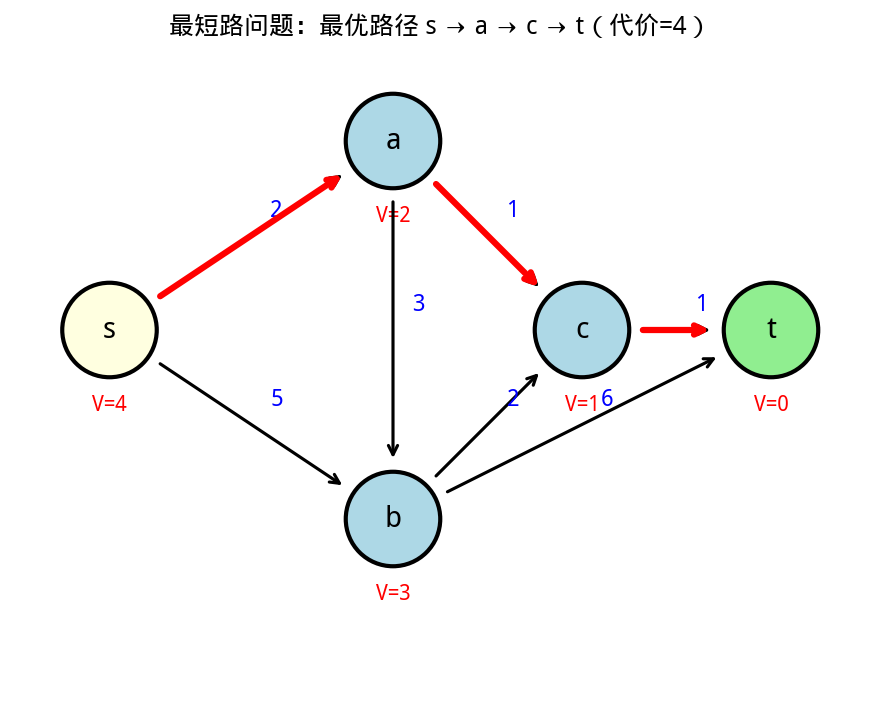
\includegraphics[width=0.6\textwidth]{figs/chap10_shortest_path.png}
\caption{最短路问题示意图。红色箭头标示最优路径$s \to a \to c \to t$，总代价为4。每个节点旁标注的$V$值是从该点到终点的最短距离。}
\label{fig:shortest_path}
\end{figure}

\subsection{最短路的线性规划形式}

最短路问题可以写成一个优雅的\textbf{线性规划}。这个视角将帮助我们深入理解求解算法的本质。

\subsubsection{原始问题：流量视角}

想象每条边上有"流量"$x_{ij}$。我们要把一单位的流量从$s$送到$t$，使得总代价最小：

\begin{equation}
    \begin{aligned}
        \min_{x} \quad & \sum_{(i,j) \in E} w_{ij} \cdot x_{ij} \\
        \text{s.t.} \quad & \sum_{j} x_{ij} - \sum_{k} x_{ki} = \begin{cases}
            1 & \text{if } i = s \\
            -1 & \text{if } i = t \\
            0 & \text{otherwise}
        \end{cases} \\
        & x_{ij} \geq 0, \quad \forall (i,j) \in E
    \end{aligned}
\end{equation}

这里的约束叫做\textbf{流量守恒}：除了起点（流出1单位）和终点（流入1单位），其他每个顶点流入等于流出。

\subsubsection{对偶问题：势能视角}

现在我们来写这个线性规划的对偶问题。

为每个顶点 $i$ 的流量守恒约束引入对偶变量 $V_i$（你可以把它想象成顶点的"势能"或"位置"）。根据线性规划对偶理论，对偶问题是：

\begin{keyformula}[title=最短路的对偶问题]
\begin{equation}
    \begin{aligned}
        \max_{V} \quad & V_t - V_s \\
        \text{s.t.} \quad & V_j - V_i \leq w_{ij}, \quad \forall (i,j) \in E
    \end{aligned}
\end{equation}
\end{keyformula}

\paragraph{物理直觉：绳网模型}

这个对偶问题有一个美妙的物理解释。想象每条边 $(i,j)$ 是一根\textbf{长度为 $w_{ij}$ 的绳子}，连接顶点 $i$ 和 $j$。现在：

\begin{itemize}
    \item 把起点 $s$ 固定在左边的墙壁上
    \item 把终点 $t$ 尽可能向右拉
    \item 绳子不能被拉断——相邻顶点的水平距离不能超过绳长
\end{itemize}

你能把 $t$ 拉到离墙多远？答案正是从 $s$ 到 $t$ 的最短路长度！

\begin{figure}[h]
\centering
\begin{tikzpicture}[scale=1.1]
    % 距离标尺
    \draw[->] (0,-3) -- (8.5,-3) node[right] {势能 $V$};
    \foreach \x in {0,1,2,3,4} {
        \draw (\x*2,-3.1) -- (\x*2,-2.9) node[below=2pt] {\small \x};
    }
    
    % 松弛的绳子（用抛物线/悬链线表示下垂）
    % s -> b: 绳长5，水平距离1，大量松弛
    \draw[thick, blue!60, decorate, decoration={snake, amplitude=0pt}] 
        (0,0) .. controls (0.5,-1.5) and (1.5,-2) .. (2,-1.5);
    \node[blue!60] at (0.6,-1.3) {\small $w=5$};
    
    % a -> b: 绳长3，松弛
    \draw[thick, blue!60] 
        (4,0) .. controls (3.5,-0.8) and (2.5,-1.2) .. (2,-1.5);
    \node[blue!60] at (2.7,-0.6) {\small $w=3$};
    
    % b -> c: 绳长2，水平距离2，轻微松弛
    \draw[thick, blue!60] 
        (2,-1.5) .. controls (3,-1.8) and (5,-0.8) .. (6,0);
    \node[blue!60] at (4,-1.5) {\small $w=2$};
    
    % b -> t: 绳长6，水平距离3，大量松弛
    \draw[thick, blue!60] 
        (2,-1.5) .. controls (4,-2.5) and (6,-1.5) .. (8,0);
    \node[blue!60] at (5.5,-2.3) {\small $w=6$};
    
    % 顶点（先画顶点，再画线和标签，确保标签在最上层）
    \node[circle, draw, fill=blue!20, minimum size=10mm] (s) at (0,0) {$s$};
    \node[circle, draw, fill=white, minimum size=10mm] (a) at (4,0) {$a$};
    \node[circle, draw, fill=white, minimum size=10mm] (b) at (2,-1.5) {$b$};
    \node[circle, draw, fill=white, minimum size=10mm] (c) at (6,0) {$c$};
    \node[circle, draw, fill=green!20, minimum size=10mm] (t) at (8,0) {$t$};

    % 拉紧的绳子（水平直线）- 最短路径，在节点之间
    \draw[red, very thick] (s.east) -- (a.west);
    \draw[red, very thick] (a.east) -- (c.west);
    \draw[red, very thick] (c.east) -- (t.west);

    % 拉紧标签（放在线的上方，避开节点）
    \node[red, fill=white, inner sep=1pt] at (2,0.25) {\scriptsize $w=2$};
    \node[red, fill=white, inner sep=1pt] at (5,0.25) {\scriptsize $w=1$};
    \node[red, fill=white, inner sep=1pt] at (7,0.25) {\scriptsize $w=1$};
    
    % 势能标注
    \node[above] at (0,0.6) {$V_s = 0$};
    \node[above] at (4,0.6) {$V_a = 2$};
    \node[below] at (2,-2.1) {$V_b = 1$};
    \node[above] at (6,0.6) {$V_c = 3$};
    \node[above] at (8,0.6) {$V_t = 4$};
    
    % 固定墙壁（左）
    \fill[gray!40] (-0.8,-2.5) rectangle (-0.5,1.5);
    \draw[thick] (-0.5,-2.5) -- (-0.5,1.5);
    \foreach \y in {-2,-1.5,...,1} {
        \draw[thick] (-0.8,\y) -- (-0.5,\y+0.3);
    }
    
    % 固定点
    \draw[thick] (-0.5,0) -- (0,0);
    \node[left] at (-0.8,0) {\small 固定};
    
    % 向右拉的箭头
    \draw[->, very thick, red!70] (8.6,0) -- (9.4,0) node[right] {拉！};
    
\end{tikzpicture}
\caption{绳网模型：把 $s$ 固定在墙壁，向右拉 $t$。红色的边被完全拉紧成水平直线，构成最短路径 $s \to a \to c \to t$。蓝色的边是松弛的，自然下垂。$t$ 到墙壁的水平距离（$4$）就是最短路长度。}
\label{fig:rope-network}
\end{figure}

\paragraph{为什么这是对的？}

\begin{itemize}
    \item \textbf{约束 $V_j - V_i \leq w_{ij}$}：绳子的长度限制。如果 $j$ 比 $i$ 向右超出绳长 $w_{ij}$，绳子就会被拉断。
    
    \item \textbf{目标 $\max(V_t - V_s)$}：我们想把 $t$ 拉得尽可能远离墙壁。
    
    \item \textbf{最优解}：当我们把 $t$ 拉到极限时，从 $s$ 到 $t$ 必有一条"全部拉紧"的路径——沿着这条路径，每根绳子都水平绑紧，即 $V_j - V_i = w_{ij}$。把这些等式沿路径相加：
    \[
        V_t - V_s = \sum_{\text{路径上的边}} w_{ij}
    \]
    这正是路径的总长度！而且因为其他路径的绳子在下垂（没拉紧），这条路径一定是最短的。
\end{itemize}

\begin{remark}
这个绳网模型揭示了最短路问题的\textbf{对偶结构}：
\begin{itemize}
    \item \textbf{原问题}（流的视角）：寻找从 $s$ 到 $t$ 的最小代价流
    \item \textbf{对偶问题}（势能视角）：寻找满足"绳长约束"的最大水平距离
\end{itemize}
强对偶定理告诉我们：最小流量代价 $=$ 最大势能差。这个等式在图 \ref{fig:rope-network} 中的体现是：$t$ 能被拉到的距离（$4$）恰好等于最短路的长度（$4$）。
\end{remark}

\paragraph{紧致条件与最短路径}

在最优解中，哪些边的约束取等号（$V_j - V_i = w_{ij}$）？正是\textbf{最短路径上的边}！

这些边在图中被完全拉成水平直线——水平距离恰好等于绳长。回到我们的例子：
\begin{align*}
    V_a - V_s &= 2 - 0 = 2 = w_{sa} \quad \text{（水平拉紧 }\checkmark\text{）} \\
    V_c - V_a &= 3 - 2 = 1 = w_{ac} \quad \text{（水平拉紧 }\checkmark\text{）} \\
    V_t - V_c &= 4 - 3 = 1 = w_{ct} \quad \text{（水平拉紧 }\checkmark\text{）}
\end{align*}

而非最短路径上的边则是松弛下垂的：
\begin{align*}
    V_b - V_s &= 1 - 0 = 1 < 5 = w_{sb} \quad \text{（下垂，剩余长度 $4$）} \\
    V_t - V_b &= 4 - 1 = 3 < 6 = w_{bt} \quad \text{（下垂，剩余长度 $3$）}
\end{align*}

这给了我们一个识别最短路径的方法：找到那些被水平拉紧的边，它们串起来就是最短路径。

\begin{remark}
松弛变量的物理意义也很清楚：它是绳子的\textbf{下垂量}（更准确地说，是绳长减去水平投影的差值）。绳子下垂得越厉害，说明这条边离"最短路"越远。如果 $V_b - V_s = 1$ 而 $w_{sb} = 5$，说明这根绳子还可以再水平拉伸 $4$ 个单位才会绑紧——这告诉我们走 $s \to b$ 这条路，后面还需要额外 $4$ 的代价才能"追上"最短路径。
\end{remark}
% ------------------------------------------------------------------------------------
\section{两种求解思路：对偶上升与原始改进}
% ------------------------------------------------------------------------------------

现在我们有了最短路问题的原始-对偶结构。如何求解？

有两种根本不同的策略，它们对应着你可能听说过的两类算法。

\subsection{策略一：对偶上升——维护最优性}

\textbf{核心思想}：从势能函数$V$出发，始终保持$V$满足所有约束（对偶可行），逐步提升目标$V_t - V_s$。

想象你是一个"保守派"：你不愿意冒险，每一步都要确保自己的解是"合法"的。

具体做法：
\begin{enumerate}
    \item 初始化：$V_t = 0$，其他$V_i = -\infty$（或者某个很小的值）
    \item 找到一个可以"提升"的顶点：存在边$(i,j)$使得$V_i < V_j - w_{ij}$
    \item 更新：$V_i \leftarrow V_j - w_{ij}$（让约束紧绑）
    \item 重复，直到无法再提升
\end{enumerate}

\textbf{关键性质}：每次更新都让$V_s$变大（因为势能像波浪一样从$t$向$s$传播），而且每一步的$V$都满足所有约束。

这就是\textbf{Dijkstra算法}的本质！它从终点开始，像水波一样向外扩展势能等值面。

\begin{figure}[h]
\centering
\begin{tikzpicture}[scale=0.9]
    % 波纹
    \fill[blue!10] (0,0) circle (2.5);
    \fill[blue!20] (0,0) circle (1.8);
    \fill[blue!30] (0,0) circle (1.1);
    \fill[blue!50] (0,0) circle (0.4);
    
    \node[font=\small] at (0,0) {$t$};
    \node[font=\footnotesize] at (0.8,0.8) {$V=1$};
    \node[font=\footnotesize] at (1.4,1.4) {$V=2$};
    \node[font=\footnotesize] at (2,2) {$V=3$};
    
    \node[below, font=\small] at (0,-3) {势能等值面从终点向外扩展};
\end{tikzpicture}
\caption{Dijkstra算法的几何直观：对偶上升}
\end{figure}

\subsection{策略二：原始改进——维护可行性}

\textbf{核心思想}：从一条实际路径出发，始终保持有一条从$s$到$t$的路（原始可行），逐步缩短路径长度。

想象你是一个"冒险家"：你先冲到终点再说，然后慢慢优化路线。

具体做法：
\begin{enumerate}
    \item 随便找一条从$s$到$t$的路径（可能很绕）
    \item 检查：有没有"捷径"可以替换当前路径的某一段？
    \item 如果有，更新路径
    \item 重复，直到找不到更短的路
\end{enumerate}

\textbf{关键性质}：每次更新都让路径变短，而且每一步都有一条完整的可行路径。

这就是\textbf{Bellman-Ford算法}的精神！它通过反复"松弛"所有边，让最短距离信息逐渐传播。

\subsection{两种策略的对比}

\begin{table}[h]
\centering
\caption{对偶上升 vs 原始改进}
\begin{tabular}{lcc}
\toprule
& \textbf{对偶上升（Dijkstra风格）} & \textbf{原始改进（Bellman-Ford风格）} \\
\midrule
维护什么 & 势能函数$V$（对偶变量） & 具体路径（原始变量） \\
解的状态 & 对偶可行，但可能"不完整" & 原始可行，但可能"不最优" \\
每步做什么 & 扩展确定区域 & 改进当前路径 \\
收敛时 & 对偶目标达到最优 & 原始目标达到最优 \\
界的变化 & 下界$\uparrow$上升 & 上界$\downarrow$下降 \\
\midrule
适用条件 & 需要边权非负 & 允许负边权 \\
时间复杂度 & $O(E \log V)$ & $O(VE)$ \\
\bottomrule
\end{tabular}
\end{table}

\begin{physicalmeaning}
\textbf{选择哪种策略？}

这取决于你的问题结构：
\begin{itemize}
    \item 如果约束容易满足，但找最优解难——用\textbf{对偶上升}（先保证最优，再扩展可行域）
    \item 如果找最优解容易，但满足约束难——用\textbf{原始改进}（先保证可行，再改进目标）
\end{itemize}

在最短路问题中，找一条路（原始可行）很容易，但要找最短的那条（最优）较难，所以Dijkstra（对偶上升）通常更高效。
\end{physicalmeaning}

% ------------------------------------------------------------------------------------
\section{从最短路到强化学习：算法设计的核心权衡}
% ------------------------------------------------------------------------------------

在最短路问题中，我们见识了两种截然不同的求解思路：
\begin{itemize}
    \item \textbf{深度优先}：沿着一条路走到底，看看总代价是多少，再回溯尝试其他路径
    \item \textbf{动态规划}：从终点往回推，逐步计算每个节点的最优值
\end{itemize}

这两种思路的差异，其实反映了算法设计中一个根本性的权衡。当我们从最短路走向更复杂的强化学习问题时，这个权衡会变得更加关键，同时还会出现新的挑战。

本节我们将建立一个"算法坐标系"，帮助你理解各种强化学习算法的设计逻辑。

% ------------------------------------------------------------------------------------
\subsection{核心权衡：探索深度 vs. 计算代价}
% ------------------------------------------------------------------------------------

让我们先聚焦于两个最基本的维度：\textbf{我们要探索多深}，以及\textbf{我们对环境了解多少}。

\subsubsection{维度一：更新深度——走多远再回头？}

\begin{keyidea}[title=核心问题]
更新价值函数时，我们应该走多少步再回头总结经验？
\end{keyidea}

回想最短路的两种算法：

\textbf{深度优先搜索}必须走完一整条路径才能知道这条路的代价。如果路径很长，中间有很多岔路，每条岔路又有岔路……搜索空间会指数爆炸。

\textbf{动态规划}则聪明得多：它只看"一步"。从终点开始，先算出离终点一步的节点的最优值；再算离终点两步的；依此类推。每一步都利用之前算好的结果，避免了重复计算。

这两种思路在强化学习中分别对应：

\paragraph{蒙特卡洛方法（MC）——"走到底再算账"}

就像深度优先搜索，MC方法必须完成一整个\textbf{回合}（episode），才能计算这条轨迹的总回报：
\begin{equation}
    G_t = r_t + \gamma r_{t+1} + \gamma^2 r_{t+2} + \cdots + \gamma^{T-t} r_T
\end{equation}

\paragraph{时序差分方法（TD）——"走一步就更新"}

就像动态规划，TD方法只看一步，然后用对下一状态的\textbf{估计值}来补全剩余部分：
\begin{equation}
    \text{TD目标} = r_t + \gamma \hat{V}(s_{t+1})
\end{equation}

这种"用估计更新估计"的技巧叫做\textbf{自举}（Bootstrapping）——就像拽着自己的鞋带把自己提起来。

\paragraph{直观理解：期中考 vs. 期末考}

假设你是老师，想预测学生的学习效果：

\begin{itemize}
    \item \textbf{TD思路}：期中考完就预测期末成绩。反馈快，但可能不准（有\textbf{偏差}）。
    \item \textbf{MC思路}：等期末考完再看真实成绩。绝对准确（\textbf{无偏}），但如果学生那天生病或超常发挥，结果波动很大（高\textbf{方差}）。
\end{itemize}

\begin{figure}[h]
\centering
\begin{tikzpicture}[scale=0.85, >=stealth]
    % 时间轴
    \draw[->, thick] (0,0) -- (14,0) node[right] {时间};
    
    % 状态节点
    \foreach \i/\label in {0/$s_t$, 2.5/$s_{t+1}$, 5/$s_{t+2}$, 9/$s_{t+3}$, 12.5/终点} {
        \fill (\i, 0) circle (3pt);
        \node[below] at (\i, -0.3) {\label};
    }
    \node at (7, 0) {$\cdots$};
    \node at (11, 0) {$\cdots$};
    
    % 奖励
    \foreach \i/\r in {1.25/$r_t$, 3.75/$r_{t+1}$, 6/$r_{t+2}$} {
        \node[above, blue] at (\i, 0.3) {\small \r};
    }
    
    % TD(0)：只看一步
    \draw[red, very thick, ->] (0, 1.2) -- (2.5, 1.2);
    \node[red, above] at (1.25, 1.2) {\textbf{TD(0)}};
    \node[red, right, font=\small] at (2.7, 1.2) {$r_t + \gamma \hat{V}(s_{t+1})$};
    \draw[red, dashed] (2.5, 1) -- (2.5, 0.2);
    
    % n-step
    \draw[orange, very thick, ->] (0, 2.2) -- (5, 2.2);
    \node[orange, above] at (2.5, 2.2) {\textbf{n-step TD}};
    \draw[orange, dashed] (5, 2) -- (5, 0.2);
    
    % MC：走到底
    \draw[green!60!black, very thick, ->] (0, 3.2) -- (12.5, 3.2);
    \node[green!60!black, above] at (6.25, 3.2) {\textbf{Monte Carlo}};
    \node[green!60!black, right, font=\small] at (12.7, 3.2) {$G_t = \sum \gamma^k r_{t+k}$};
    
\end{tikzpicture}
\caption{不同的更新深度：TD只看一步，n-step看若干步，MC走到终点}
\end{figure}

\subsubsection{维度二：模型依赖——能不能"想象"？}

\begin{keyidea}[title=核心问题]
我们知道环境的运作规则吗？能在脑中"推演"吗？
\end{keyidea}

回想最短路问题：我们知道图的完整结构——哪些节点相连、每条边的权重。有了这些信息，动态规划才能施展威力。

但如果你\textbf{不知道}图的结构呢？你只能从起点出发，走一步看一步，通过不断试错来摸清地形。

这就是\textbf{有模型}与\textbf{无模型}的区别：

\paragraph{有模型方法（Model-based）}

你知道（或者学会了）环境的"规则"：
\begin{itemize}
    \item 状态转移：从状态 $s$ 采取动作 $a$，会到达什么状态 $s'$？
    \item 奖励函数：这一步能获得多少奖励？
\end{itemize}

有了模型，你可以在"脑海中"推演，不需要真的和环境交互。就像下棋高手，不需要真的落子，就能在脑中预判十几步之后的局面。

\paragraph{无模型方法（Model-free）}

你对环境一无所知，只能通过\textbf{真实的试错}来学习。每次想知道某个动作好不好，都必须真的去做，承受后果。

\begin{table}[h]
\centering
\renewcommand{\arraystretch}{1.4}
\begin{tabular}{p{2.5cm}|p{5.5cm}|p{5.5cm}}
\toprule
& \textbf{有模型 (Model-based)} & \textbf{无模型 (Model-free)} \\
\midrule
\textbf{类比} & 知道棋盘规则，脑中推演 & 不知规则，只能试错 \\
\midrule
\textbf{优势} & 
数据效率极高；可以"想象"从未经历的情况；可以谨慎避免危险
 & 
实现简单；不怕模型不准；渐进性能通常更好
 \\
\midrule
\textbf{劣势} & 
模型难以精确获得；模型偏差会导致策略失效
 & 
需要海量真实交互；每次学习都要真的"摔跤"
 \\
\midrule
\textbf{代表算法} & AlphaZero、MuZero、Dreamer & DQN、PPO、SAC \\
\bottomrule
\end{tabular}
\caption{有模型 vs. 无模型方法的对比}
\end{table}

\subsubsection{二维图谱：算法的基本定位}

现在我们可以用这两个维度画出一张"算法地图"：

\begin{figure}[h]
\centering
\begin{tikzpicture}[scale=1.15, >=stealth]
    % 坐标轴
    \draw[->, very thick] (-5.2,0) -- (5.2,0);
    \draw[->, very thick] (0,-3.5) -- (0,3.8);
    
    % 轴标签
    \node[above] at (0, 3.8) {\textbf{模型依赖}};
    \node[right] at (5.2, 0) {\textbf{更新深度}};
    
    \node[below, font=\small, align=center] at (-4,0) {深 (MC)\\ \scriptsize 无偏·高方差};
    \node[below, font=\small, align=center] at (4,0) {浅 (TD)\\ \scriptsize 有偏·低方差};
    \node[left, font=\small, align=right] at (0,3) {有模型\\ \scriptsize 可以规划};
    \node[left, font=\small, align=right] at (0,-3) {无模型\\ \scriptsize 只能试错};
    
    % --- 四个象限 ---
    
    % 右上：动态规划
    \node[draw=blue!80, thick, rounded corners, fill=blue!10, text width=3cm, align=center] at (3.3, 2.3) {
        \textbf{动态规划}\\[3pt]
        \footnotesize Value Iteration\\
        Policy Iteration\\[3pt]
        \scriptsize 理论最优解
    };
    
    % 左上：规划搜索
    \node[draw=green!60!black, thick, rounded corners, fill=green!10, text width=3cm, align=center] at (-3.3, 2.3) {
        \textbf{树搜索}\\[3pt]
        \footnotesize MCTS\\
        AlphaZero\\[3pt]
        \scriptsize 围棋、国际象棋
    };
    
    % 左下：蒙特卡洛RL
    \node[draw=red!80, thick, rounded corners, fill=red!10, text width=3cm, align=center] at (-3.3, -2.3) {
        \textbf{蒙特卡洛 RL}\\[3pt]
        \footnotesize REINFORCE\\
        GRPO\\[3pt]
        \scriptsize 大模型训练
    };
    
    % 右下：时序差分RL
    \node[draw=orange!80, thick, rounded corners, fill=orange!10, text width=3cm, align=center] at (3.3, -2.3) {
        \textbf{时序差分 RL}\\[3pt]
        \footnotesize Q-Learning, DQN\\
        SARSA\\[3pt]
        \scriptsize 游戏AI
    };
    
    % 中间：Actor-Critic
    \node[draw=purple!80, thick, dashed, rounded corners, fill=purple!10, text width=3.2cm, align=center] at (0, -2.3) {
        \textbf{Actor-Critic}\\[3pt]
        \footnotesize PPO, SAC, A3C\\[3pt]
        \scriptsize 工业界主流
    };
    
    % 连接线
    \draw[dashed, gray] (-1.6, -2.3) -- (-3.3+1.5, -2.3);
    \draw[dashed, gray] (1.6, -2.3) -- (3.3-1.5, -2.3);
    
    % 对角线箭头表示权衡
    \draw[->, thick, gray, dashed] (-3.5, -3) -- (3.5, 3) node[pos=0.85, above, sloped, font=\small] {单步计算代价 $\uparrow$};
    
\end{tikzpicture}
\caption{强化学习算法的基本图谱。横轴是更新深度，纵轴是模型依赖程度。对角线方向代表计算代价的增加。}
\label{fig:rl-2d-map}
\end{figure}

\paragraph{图谱解读}

\begin{itemize}
    \item \textbf{右上角（动态规划）}：最短路问题就在这里！我们知道完整的图结构（有模型），用自举更新（TD式）。这是理论上最理想的情况——如果你能准确描述环境，动态规划给出的就是最优解。
    
    \item \textbf{左上角（树搜索）}：AlphaZero在这里。它知道棋盘规则（有模型），通过蒙特卡洛树搜索（MCTS）进行深度推演。计算量大，但效果惊人。
    
    \item \textbf{右下角（时序差分RL）}：DQN、Q-Learning在这里。不知道环境规则（无模型），只能通过试错学习，但每一步都及时更新（TD），收敛相对较快。
    
    \item \textbf{左下角（蒙特卡洛RL）}：REINFORCE、GRPO在这里。不知道模型，还必须走完整条轨迹才能更新。听起来最"笨"，但在某些场景下（如大语言模型训练）反而有独特优势。
    
    \item \textbf{中央（Actor-Critic）}：PPO、SAC等算法介于TD和MC之间，是目前工业界最常用的方法。
\end{itemize}

\begin{remark}
注意对角线方向：从右下到左上，计算代价递增。无模型+浅层更新单步最"便宜"；有模型+深度搜索单步最"昂贵"但也最强大。选择算法时，需要根据问题特点和计算预算来权衡。
\end{remark}

% ------------------------------------------------------------------------------------
\subsection{两个关键因素：数据的来源与使用}
% ------------------------------------------------------------------------------------

上面的二维图谱描述了"怎么计算"的问题。但在实际应用中，还有另一个同样重要的问题：\textbf{数据从哪来、怎么用}？

这涉及两个额外的维度，它们决定了算法的\textbf{数据效率}和\textbf{适用场景}。

\subsubsection{维度三：数据新鲜度（On-policy vs. Off-policy）}

\begin{keyidea}[title=核心问题]
训练数据必须来自当前策略吗？能不能用"过时"的数据？
\end{keyidea}

\paragraph{类比：学游泳}

你现在的游泳姿势是A，游了一圈后，教练给你反馈，你调整成姿势B。

问题来了：\textbf{刚才用姿势A游的那一圈数据，还能用来改进姿势B吗？}

\begin{itemize}
    \item \textbf{On-policy（同策略）}：不能。姿势A和姿势B的水感不同，旧数据可能产生误导。每次更新后，旧数据必须丢弃。
    
    \item \textbf{Off-policy（异策略）}：可以！通过数学技巧（如重要性采样），我们可以"修正"旧数据，使其对新策略也有参考价值。
\end{itemize}

\begin{figure}[h]
\centering
\begin{tikzpicture}[scale=0.85, >=stealth]
    % On-policy
    \begin{scope}[xshift=-5cm]
        \node[font=\bfseries] at (0, 3.2) {On-policy};
        \node[font=\small, gray] at (0, 2.7) {"数据保鲜期：一次"};
        
        \node[draw, rounded corners, fill=blue!20, minimum width=2cm, minimum height=0.7cm] (pi) at (0, 1.8) {策略 $\pi_\theta$};
        \node[draw, rounded corners, fill=green!20, minimum width=2cm, minimum height=0.7cm] (env) at (0, 0) {环境};
        \node[draw, rounded corners, fill=orange!20, minimum width=1.4cm, minimum height=0.5cm] (data) at (2.5, 0.9) {\small 数据};
        
        \draw[->, thick] (pi) -- node[left, font=\small] {交互} (env);
        \draw[->, thick] (env) -- (data);
        \draw[->, thick] (data) -- node[above, font=\small] {更新} (pi);
        
        \node[draw, rounded corners, fill=red!15, font=\small] at (2.5, -0.5) {丢弃};
        \draw[->, thick, red] (data) -- (2.5, -0.1);
    \end{scope}
    
    % Off-policy
    \begin{scope}[xshift=5cm]
        \node[font=\bfseries] at (0, 3.2) {Off-policy};
        \node[font=\small, gray] at (0, 2.7) {"数据可以反复使用"};
        
        \node[draw, rounded corners, fill=blue!20, minimum width=2cm, minimum height=0.7cm] (pi2) at (0, 1.8) {策略 $\pi_\theta$};
        \node[draw, rounded corners, fill=green!20, minimum width=2cm, minimum height=0.7cm] (env2) at (0, 0) {环境};
        \node[draw, rounded corners, fill=yellow!30, minimum width=1.8cm, minimum height=1cm] (buffer) at (2.8, 0.9) {\small 经验池};
        
        \draw[->, thick] (pi2) -- node[left, font=\small] {交互} (env2);
        \draw[->, thick] (env2) -- (buffer);
        \draw[->, thick] (buffer) -- node[above, font=\small] {采样} (pi2);
        
        \draw[->, thick, green!60!black] (buffer.south) arc (-90:180:0.25) -- (buffer.west);
        \node[green!60!black, font=\scriptsize] at (1.8, -0.1) {保留};
    \end{scope}
\end{tikzpicture}
\caption{On-policy每次更新后丢弃数据，Off-policy把数据存入经验池反复使用}
\end{figure}

\begin{table}[h]
\centering
\renewcommand{\arraystretch}{1.3}
\begin{tabular}{p{2.5cm}|p{5.2cm}|p{5.2cm}}
\toprule
& \textbf{On-policy} & \textbf{Off-policy} \\
\midrule
\textbf{数据要求} & 必须是当前策略产生的 & 可以是任意策略产生的 \\
\textbf{数据利用} & 用一次就丢弃 & 存入经验池，反复使用 \\
\textbf{优势} & 理论简洁，训练稳定 & 数据效率高 \\
\textbf{劣势} & 浪费数据 & 需要额外技巧保证稳定 \\
\textbf{代表} & PPO, REINFORCE, GRPO & DQN, SAC, TD3 \\
\bottomrule
\end{tabular}
\caption{On-policy vs. Off-policy}
\end{table}

\subsubsection{维度四：交互模式（Online vs. Offline）}

\begin{keyidea}[title=核心问题]
训练时能不能和环境实时交互？还是只能用已有的历史数据？
\end{keyidea}

这个维度在大模型时代变得尤为重要。

\paragraph{类比：学开车}

\begin{itemize}
    \item \textbf{Online（在线学习）}：你坐在真车里，边开边学。教练随时给反馈，你随时调整。
    
    \item \textbf{Offline（离线学习）}：你不能碰车。只能看一大堆别人的行车记录视频，从中学习。
\end{itemize}

\begin{figure}[h]
\centering
\begin{tikzpicture}[scale=0.85, >=stealth]
    % Online
    \begin{scope}[xshift=-5cm]
        \node[font=\bfseries] at (0, 2.8) {Online};
        \node[font=\small, gray] at (0, 2.3) {"边做边学"};
        
        \node[draw, rounded corners, fill=blue!20, minimum width=2cm, minimum height=0.7cm] (agent) at (0, 1.2) {智能体};
        \node[draw, rounded corners, fill=green!20, minimum width=2cm, minimum height=0.7cm] (env) at (0, -0.8) {环境};
        
        \draw[->, thick] (agent.south west) -- node[left, font=\small] {动作} (env.north west);
        \draw[->, thick] (env.north east) -- node[right, font=\small] {反馈} (agent.south east);
        
        \node[font=\scriptsize, gray] at (0, -1.8) {可以实时交互};
    \end{scope}
    
    % Offline
    \begin{scope}[xshift=5cm]
        \node[font=\bfseries] at (0, 2.8) {Offline};
        \node[font=\small, gray] at (0, 2.3) {"只看不做"};
        
        \node[draw, rounded corners, fill=blue!20, minimum width=2cm, minimum height=0.7cm] (agent2) at (0, 1.2) {智能体};
        \node[draw, rounded corners, fill=gray!30, minimum width=2.5cm, minimum height=1cm] (data) at (0, -0.8) {\small 历史数据集};
        
        \draw[->, thick] (data) -- node[right, font=\small] {学习} (agent2);
        
        \node[draw, rounded corners, fill=green!10, minimum width=1.5cm, minimum height=0.5cm] (env2) at (3, -0.8) {\small 环境};
        \draw[thick, red] (agent2.east) -- ++(0.5,0) -- ++(0,-1.3) node[midway, right, font=\scriptsize, red] {禁止} -- (env2.north);
        \draw[red, thick] (2.2, -0.3) -- (2.6, -0.7);
        \draw[red, thick] (2.2, -0.7) -- (2.6, -0.3);
        
        \node[font=\scriptsize, gray] at (0, -2) {不能和环境交互};
    \end{scope}
\end{tikzpicture}
\caption{Online可以实时与环境交互，Offline只能从固定数据集学习}
\end{figure}

\paragraph{为什么需要Offline RL？}

在很多实际场景中，我们\textbf{无法}进行在线交互：

\begin{itemize}
    \item \textbf{医疗}：不能让AI在真实病人身上"试错"
    \item \textbf{自动驾驶}：让一辆不会开车的AI上路太危险
    \item \textbf{推荐系统}：随意推荐会损失用户和收入
    \item \textbf{大模型对齐}：每次生成都要人类标注太昂贵
\end{itemize}

但我们通常有大量的\textbf{历史数据}：过去的诊疗记录、人类司机的驾驶日志、用户的点击历史、人类写的高质量文本……

Offline RL的目标就是：\textbf{只用这些历史数据，不做任何新的交互，训练出好的策略}。

\begin{table}[h]
\centering
\renewcommand{\arraystretch}{1.3}
\begin{tabular}{p{2.5cm}|p{5.2cm}|p{5.2cm}}
\toprule
& \textbf{Online} & \textbf{Offline} \\
\midrule
\textbf{数据来源} & 实时与环境交互产生 & 固定的历史数据集 \\
\textbf{能否探索} & 可以尝试新动作 & 只能用数据中出现过的 \\
\textbf{优势} & 可以主动探索最优策略 & 安全、成本低 \\
\textbf{核心挑战} & 探索的代价（安全/成本） & 分布偏移（数据不够多样） \\
\textbf{代表} & DQN, PPO, SAC & CQL, IQL, Decision Transformer \\
\bottomrule
\end{tabular}
\caption{Online vs. Offline：交互模式的权衡}
\end{table}

\begin{example}[title=大模型训练中的Online vs. Offline]
训练ChatGPT这样的对话模型时：

\textbf{Offline阶段}：用大量人类写的文本做预训练（SFT）。这是纯Offline的——模型只是"看"人类怎么写，自己不产生任何输出。

\textbf{Online阶段}：RLHF训练时，模型生成回答，人类给反馈，模型根据反馈调整。这是Online的——模型在"边做边学"。

实际中，由于人类标注昂贵，很多工作探索如何用更少的Online交互，更多地利用Offline数据。
\end{example}

\begin{remark}
On/Off-policy 和 Online/Offline 是两个不同的维度，容易混淆：
\begin{itemize}
    \item \textbf{On/Off-policy}：问的是"数据是不是当前策略产生的"
    \item \textbf{Online/Offline}：问的是"能不能边和环境交互边训练"
\end{itemize}
一个Off-policy算法（如DQN）通常用于Online场景；而Offline RL是一个独立的研究领域，需要专门设计的算法（如CQL）。
\end{remark}

% ------------------------------------------------------------------------------------
\section{算法全景：四维定位与选择指南}
% ------------------------------------------------------------------------------------

现在我们有了四个维度，可以像GPS定位一样精确地描述任何强化学习算法。
\marginnote{\textbf{为什么DeepSeek选择MC方法？}

传统RL中MC因高方差被避免，但大模型场景有特殊性：
\begin{enumerate}
    \item 答案对错明确（如数学题）
    \item Critic网络训练成本极高
    \item 可并行采样多条轨迹降低方差
\end{enumerate}
这使"古老"的蒙特卡洛方法焕发新生。
}

\subsection{主流算法的四维属性表}

\begin{table}[htbp]
\centering
\small
\renewcommand{\arraystretch}{1.35}
\caption{主流强化学习算法的四维定位（第一部分）}
\begin{tabular}{l|c|c|c|c|p{3.5cm}}
\toprule
\textbf{算法} & \textbf{模型} & \textbf{深度} & \textbf{新鲜度} & \textbf{交互} & \textbf{典型应用} \\
\midrule
\multicolumn{6}{l}{\textit{经典基础}} \\
\midrule
Q-Learning & 无 & TD & Off-policy & Online & 理论基石 \\
SARSA & 无 & TD & On-policy & Online & Q-Learning的保守版 \\
REINFORCE & 无 & MC & On-policy & Online & 最纯粹的策略梯度 \\
\midrule
\multicolumn{6}{l}{\textit{深度强化学习}} \\
\midrule
DQN & 无 & TD & Off-policy & Online & Atari游戏 \\
PPO & 无 & n-step & On-policy & Online & \textbf{ChatGPT}、机器人 \\
SAC & 无 & TD & Off-policy & Online & 机器人控制 \\
TD3 & 无 & TD & Off-policy & Online & 连续控制 \\
\bottomrule
\end{tabular}
\end{table}

\begin{table}[htbp]
\centering
\small
\renewcommand{\arraystretch}{1.35}
\caption{主流强化学习算法的四维定位（第二部分）}
\begin{tabular}{l|c|c|c|c|p{3.5cm}}
\toprule
\textbf{算法} & \textbf{模型} & \textbf{深度} & \textbf{新鲜度} & \textbf{交互} & \textbf{典型应用} \\
\midrule
\multicolumn{6}{l}{\textit{有模型方法}} \\
\midrule
AlphaZero & 有 & MCTS & Off-policy & Online & 围棋、国际象棋 \\
MuZero & 学习 & MCTS & Off-policy & Online & 不知规则的游戏 \\
Dreamer & 学习 & 想象 & On-policy & Online & 视觉控制任务 \\
\midrule
\multicolumn{6}{l}{\textit{大模型对齐}} \\
\midrule
RLHF (PPO) & 无 & n-step & On-policy & Online & \textbf{ChatGPT}对齐 \\
GRPO & 无 & MC & On-policy & Online & \textbf{DeepSeek}推理 \\
DPO & 无 & -- & Off-policy & Offline & 无需奖励模型的对齐 \\
\midrule
\multicolumn{6}{l}{\textit{离线强化学习}} \\
\midrule
CQL & 无 & TD & Off-policy & Offline & 医疗、机器人离线学习 \\
IQL & 无 & TD & Off-policy & Offline & 离线控制 \\
BC & 无 & -- & -- & Offline & 模仿学习基线 \\
\bottomrule
\end{tabular}
\end{table}




\subsection{如何选择算法？}

\begin{lstlisting}[style=decision, caption={强化学习算法选择指南}]
def 选择算法(问题):
    
    # 第一步：能否在线交互？
    if 不能和环境实时交互（安全/成本限制）:
        if 只有专家演示数据:
            return 行为克隆 / IQL
        else:
            return CQL / Decision Transformer
    
    # 第二步：有没有环境模型？
    if 有精确的模拟器或已知规则:
        return AlphaZero / MCTS / MuZero
    
    # 第三步：动作空间类型？
    if 动作是离散的（如游戏按键）:
        return DQN / Rainbow
    
    # 第四步：连续动作的权衡
    if 动作是连续的（如机械臂角度）:
        if 优先训练稳定性:
            return PPO  # 默认选择
        if 优先数据效率:
            return SAC / TD3
    
    # 第五步：大模型场景
    if 训练大语言模型:
        if 有人类偏好数据但不想训练RM:
            return DPO
        if 显存受限:
            return GRPO
        else:
            return PPO  # OpenAI的选择
    
    # 兜底
    return PPO  # 不知道选什么？先试PPO
\end{lstlisting}

\begin{remark}
在实际工程中，\textbf{PPO}是最安全的起点。它可能不是任何单一指标上的最优，但它在几乎所有任务上都能给出不错的结果，而且调参相对容易。先用PPO建立baseline，再根据需要尝试其他算法，是一个明智的策略。
\end{remark}

% -------------------------------------------------------------------------
\section{代码示例：值迭代与 Q-Learning}
% ------------------------------------------------------------------------------------

为了让大家更直观地理解"\textbf{需要环境模型的最优控制}（值迭代）"
和"\textbf{不需要模型的强化学习}（Q-Learning）"之间的区别，
我们用一个 5×5 的简单格子世界（GridWorld）演示。

智能体要从左上角 $(0,0)$ 出发，走到右下角 $(4,4)$。
每走一步都会损失 $1$ 的奖励（即奖励为 $-1$），
因此最短路径等价于最大化奖励。

\begin{figure}[h]
\centering
\begin{tikzpicture}[scale=0.9]
    % 画网格
    \draw[step=1, gray!50, thin] (0,0) grid (5,5);

    % 起点背景
    \fill[blue!30] (0,4) rectangle (1,5);
    % 起点标签移到左上方
    \node[font=\scriptsize, blue!70!black] at (-0.3, 4.8) {起点};

    % 终点
    \fill[green!30] (4,0) rectangle (5,1);
    \node[font=\small\bfseries] at (4.5, 0.5) {终点};

    % 智能体（红色圆圈表示当前位置）
    \node[circle, fill=red!70, minimum size=0.5cm] at (0.5, 4.5) {};

    % 坐标标注
    \node[above, font=\scriptsize] at (0.5, 5) {$(0,0)$};
    \node[below, font=\scriptsize] at (4.5, 0) {$(4,4)$};

    % 动作箭头示意
    \begin{scope}[xshift=7cm, yshift=2.5cm]
        \node[font=\bfseries] at (0, 1.8) {四个动作};
        \draw[->, thick] (0, 0.5) -- (0, 1.1) node[above, font=\small] {上};
        \draw[->, thick] (0, 0.5) -- (0, -0.1) node[below, font=\small] {下};
        \draw[->, thick] (0, 0.5) -- (-0.6, 0.5) node[left, font=\small] {左};
        \draw[->, thick] (0, 0.5) -- (0.6, 0.5) node[right, font=\small] {右};
        \fill[red!70] (0, 0.5) circle (0.15);
    \end{scope}

    % 奖励说明
    \begin{scope}[xshift=7cm, yshift=-0.5cm]
        \node[font=\small, align=left] at (0, 0) {
            每走一步：$r = -1$\\
            目标：最短路径到终点
        };
    \end{scope}

\end{tikzpicture}
\caption{5×5 GridWorld 环境。智能体（红色）从起点出发，每一步获得 $-1$ 奖励，目标是尽快到达终点。}
\end{figure}

\subsection{环境定义}

在代码中，环境就是一个函数：输入当前状态和动作，输出下一状态与奖励。

\begin{lstlisting}[language=Python]
class GridWorld:
    """5x5 网格世界"""
    def __init__(self, size=5):
        self.size = size
        self.goal = (size-1, size-1)          # 终点位置
        self.actions = [(-1,0), (1,0), (0,-1), (0,1)]  # 上、下、左、右
    
    def step(self, state, action):
        """执行动作，返回 (新状态, 奖励, 是否结束)"""
        i, j = state
        di, dj = self.actions[action]
        
        # 移动（撞墙则停在原地）
        ni = max(0, min(i + di, self.size - 1))
        nj = max(0, min(j + dj, self.size - 1))
        new_state = (ni, nj)
        
        reward = -1                            # 每一步代价为 1
        done = (new_state == self.goal)        # 到达终点则结束
        return new_state, reward, done
\end{lstlisting}

这和我们在数学上写的转移方程是一样的：
\[
s_{t+1} = f(s_t, a_t), \qquad r_t = r(s_t, a_t)
\]

% ------------------------------------------------------------------------------------
\subsection{值迭代：在脑中推演所有可能}
% ------------------------------------------------------------------------------------

值迭代是一种\textbf{有模型}方法。因为我们可以直接调用 \texttt{env.step()} 来"想象"每个动作的后果，所以不需要真的和环境交互。

\begin{figure}[h]
\centering
\begin{tikzpicture}[scale=0.75]
    % 标题
    \node[font=\bfseries] at (2.5, 6.2) {值迭代：遍历所有格子};
    
    % 画网格
    \draw[step=1, gray!50, thin] (0,0) grid (5,5);
    
    % 当前正在计算的格子
    \fill[yellow!50] (1,3) rectangle (2,4);
    \node[font=\small] at (1.5, 3.5) {$V(s)$};
    
    % 四个可能的下一步
    \draw[->, thick, blue] (1.5, 3.5) -- (1.5, 4.3) node[above, font=\scriptsize] {$r + \gamma V$};
    \draw[->, thick, blue] (1.5, 3.5) -- (1.5, 2.7) node[below, font=\scriptsize] {$r + \gamma V$};
    \draw[->, thick, blue] (1.5, 3.5) -- (0.7, 3.5) node[left, font=\scriptsize] {$r + \gamma V$};
    \draw[->, thick, blue] (1.5, 3.5) -- (2.3, 3.5) node[right, font=\scriptsize] {$r + \gamma V$};
    
    % 终点
    \fill[green!30] (4,0) rectangle (5,1);
    \node[font=\scriptsize] at (4.5, 0.5) {$V=0$};
    
    % 说明
    \begin{scope}[xshift=6.5cm, yshift=2.5cm]
        \node[align=left, font=\small] at (0, 0) {
            对每个格子 $s$：\\[3pt]
            1. 枚举 4 个动作\\
            2. 用模型算出 $s', r$\\
            3. 计算 $Q = r + \gamma V(s')$\\
            4. 取最大：$V(s) = \max_a Q$
        };
    \end{scope}
\end{tikzpicture}
\caption{值迭代在每个格子上"想象"四个方向的后果，选择最优的那个更新 $V(s)$。}
\end{figure}

\begin{lstlisting}[language=Python]
def value_iteration(env, gamma=1.0, threshold=1e-6):
    """
    值迭代算法
    - 输入：环境模型 env（可以调用 env.step 模拟任意动作）
    - 输出：最优值函数 V(s)
    """
    V = np.zeros((env.size, env.size))  # 初始化 V(s) = 0
    
    for iteration in range(1000):
        delta = 0  # 记录本轮最大变化
        
        # === 遍历所有状态 ===
        for i in range(env.size):
            for j in range(env.size):
                if (i,j) == env.goal:
                    continue  # 终点 V=0，不用更新
                
                state = (i, j)
                old_v = V[i, j]
                
                # === 枚举所有动作，用模型"想象"结果 ===
                q_values = []
                for action in range(4):
                    # 关键：这里调用模型，但不是真的执行！
                    next_state, reward, _ = env.step(state, action)
                    q = reward + gamma * V[next_state]
                    q_values.append(q)
                
                # === Bellman 最优方程：取最大值 ===
                V[i, j] = max(q_values)
                delta = max(delta, abs(old_v - V[i, j]))
        
        # 收敛判断
        if delta < threshold:
            print(f"值迭代：{iteration+1} 轮后收敛")
            break
    
    return V
\end{lstlisting}

\paragraph{算法要点}
\begin{itemize}
    \item \textbf{每轮迭代}：遍历全部 $5 \times 5 = 25$ 个状态
    \item \textbf{每个状态}：枚举 4 个动作，用模型计算 $Q(s,a) = r + \gamma V(s')$
    \item \textbf{更新规则}：$V(s) \leftarrow \max_a Q(s,a)$（Bellman 最优方程）
    \item \textbf{收敛条件}：所有状态的值变化小于阈值
    \item \textbf{计算量}：每轮 $25 \times 4 = 100$ 次模型调用，约 9 轮收敛
\end{itemize}

\begin{figure}[h]
\centering
\begin{minipage}{0.48\textwidth}
    \centering
    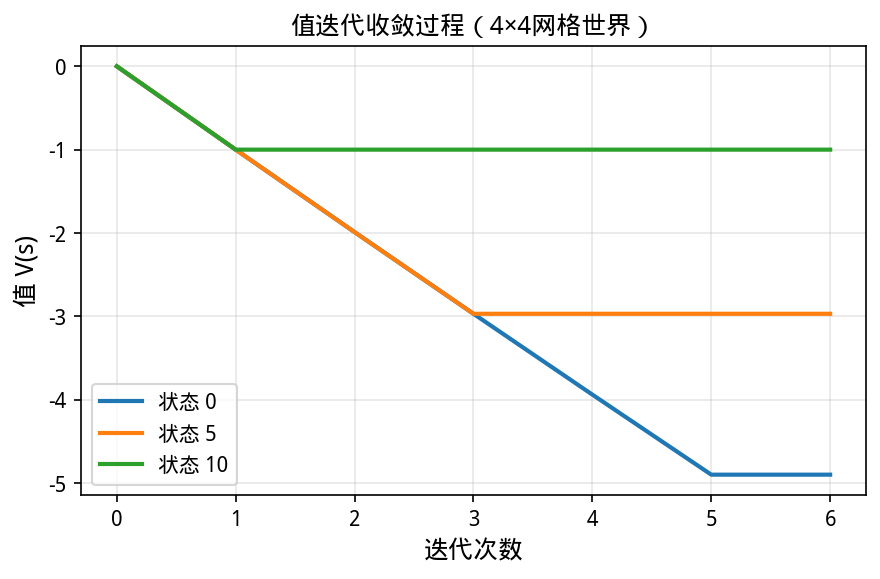
\includegraphics[width=\textwidth]{figs/chap10_value_iteration.png}
\end{minipage}
\hfill
\begin{minipage}{0.48\textwidth}
    \centering
    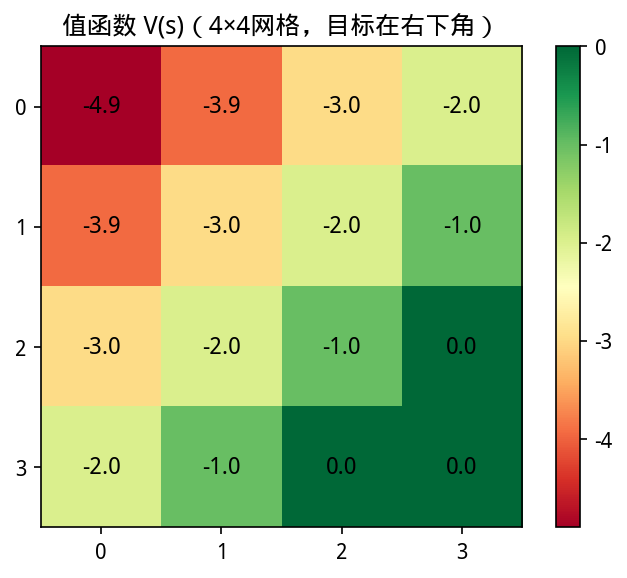
\includegraphics[width=\textwidth]{figs/chap10_value_heatmap.png}
\end{minipage}
\caption{值迭代结果。\textbf{左}：不同状态的值函数随迭代次数的变化，展示收敛过程；\textbf{右}：收敛后的值函数热力图，颜色越绿表示到达目标的期望回报越高。}
\label{fig:value_iteration}
\end{figure}

\begin{figure}[h]
\centering
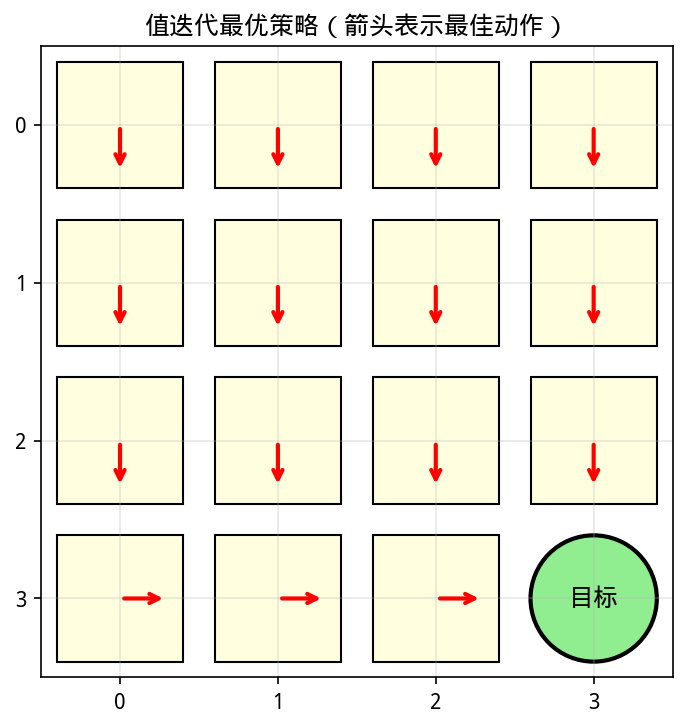
\includegraphics[width=0.45\textwidth]{figs/chap10_policy.png}
\caption{值迭代得到的最优策略。箭头指向每个状态应采取的最佳动作，指引智能体沿最短路径到达右下角的目标。}
\label{fig:policy}
\end{figure}

% ------------------------------------------------------------------------------------
\subsection{Q-Learning：从试错中学习}
% ------------------------------------------------------------------------------------

\marginnote{\textbf{Q-Learning的诞生}：Q-Learning由剑桥大学博士生Christopher Watkins在1989年博士论文中提出，1992年与Peter Dayan合作发表于\textit{Machine Learning}期刊。论文证明了Q-Learning在一定条件下收敛到最优Q函数，这个简洁的算法成为后来深度强化学习的基石。}

Q-Learning 是一种\textbf{无模型}方法。它不知道执行动作会发生什么，只能像小孩学走路一样——走一步、摔一跤、记住教训。

\begin{figure}[h]
\centering
\begin{tikzpicture}[scale=0.75]
    % 标题
    \node[font=\bfseries] at (2.5, 6.2) {Q-Learning：边走边学};
    
    % 画网格
    \draw[step=1, gray!50, thin] (0,0) grid (5,5);
    
    % 一条轨迹
    \fill[blue!20] (0,4) rectangle (1,5);
    \fill[blue!20] (1,4) rectangle (2,5);
    \fill[blue!20] (1,3) rectangle (2,4);
    \fill[blue!20] (2,3) rectangle (3,4);
    \fill[blue!20] (2,2) rectangle (3,3);
    
    % 轨迹箭头
    \draw[->, very thick, red!70] (0.5, 4.5) -- (1.3, 4.5);
    \draw[->, very thick, red!70] (1.5, 4.5) -- (1.5, 3.7);
    \draw[->, very thick, red!70] (1.5, 3.5) -- (2.3, 3.5);
    \draw[->, very thick, red!70] (2.5, 3.5) -- (2.5, 2.7);
    
    % 当前位置
    \node[circle, fill=red!70, minimum size=0.5cm] at (2.5, 2.5) {};
    
    % 终点
    \fill[green!30] (4,0) rectangle (5,1);
    
    % 说明
    \begin{scope}[xshift=6.5cm, yshift=2.5cm]
        \node[align=left, font=\small] at (0, 0) {
            每一步：\\[3pt]
            1. 选动作（探索/利用）\\
            2. 执行，观察 $s', r$\\
            3. 计算 TD 误差\\
            4. 更新 $Q(s,a)$\\
            5. 移动到 $s'$
        };
    \end{scope}
\end{tikzpicture}
\caption{Q-Learning 通过实际走动来学习。红色箭头表示智能体走过的轨迹，每走一步就更新一次 $Q$ 值。}
\end{figure}

\begin{lstlisting}[language=Python]
def q_learning(env, episodes=2000, gamma=1.0, alpha=0.1, epsilon=0.1):
    """
    Q-Learning 算法
    - 输入：环境 env（只能通过交互获取信息）
    - 输出：学到的 Q(s,a) 函数
    - 超参数：
        - episodes: 训练回合数
        - alpha: 学习率（每次更新的步长）
        - epsilon: 探索概率
    """
    Q = np.zeros((env.size, env.size, 4))  # Q(s, a) 初始化为 0
    
    for episode in range(episodes):
        state = (0, 0)  # 每个回合从起点开始
        
        # === 一个回合：从起点走到终点 ===
        while True:
            # --- 第一步：选择动作（epsilon-贪婪）---
            if np.random.random() < epsilon:
                action = np.random.randint(4)      # 10% 概率随机探索
            else:
                action = np.argmax(Q[state[0], state[1]])  # 90% 选当前最优；注意python张量特性
            
            # --- 第二步：执行动作，观察结果 ---
            # 注意：这是真实交互，不是模拟！
            next_state, reward, done = env.step(state, action)
            
            # --- 第三步：计算 TD 目标和误差 ---
            if done:
                td_target = reward  # 终点没有未来
            else:
                td_target = reward + gamma * np.max(Q[next_state])
            
            td_error = td_target - Q[state[0], state[1], action]
            
            # --- 第四步：更新 Q 值 ---
            # Q(s,a) ← Q(s,a) + α * (TD目标 - Q(s,a))
            Q[state[0], state[1], action] += alpha * td_error
            
            # --- 第五步：移动到下一状态 ---
            state = next_state
            if done:
                break  # 到达终点，结束本回合
    
    print(f"Q-Learning：训练了 {episodes} 个回合")
    return Q
\end{lstlisting}

\paragraph{算法要点}
\begin{itemize}
    \item \textbf{每个回合}：从起点走到终点，大约 8-20 步（取决于探索）
    \item \textbf{每一步}：只更新当前 $(s, a)$ 对应的 $Q$ 值（而不是所有状态）
    \item \textbf{探索 vs 利用}：$\epsilon = 0.1$ 意味着 10\% 概率随机探索，90\% 选当前最优
    \item \textbf{学习率}：$\alpha = 0.1$ 控制每次更新的幅度
    \item \textbf{计算量}：2000 回合 $\times$ 平均 10 步 $=$ 约 20000 次真实交互
\end{itemize}

\begin{figure}[h]
\centering
\begin{tikzpicture}[>=stealth]
    % TD 更新公式可视化
    \node[draw, rounded corners, fill=blue!10, minimum width=2.5cm, minimum height=1cm] (old) at (0, 0) {$Q(s,a)$};
    \node[draw, rounded corners, fill=green!10, minimum width=4cm, minimum height=1cm] (target) at (6, 0) {$r + \gamma \max_{a'} Q(s',a')$};
    \node[draw, rounded corners, fill=orange!10, minimum width=2.5cm, minimum height=1cm] (new) at (3, -2) {$Q(s,a)_{new}$};
    
    \draw[->, thick] (old) -- node[above] {TD 误差} (target);
    \draw[->, thick] (old) -- node[left] {$+ \alpha \cdot$} (new);
    \draw[->, thick] (target) -- node[right] {误差} (new);
    
    \node[below, font=\small, gray] at (3, -3) {$Q(s,a) \leftarrow Q(s,a) + \alpha \cdot \big[ \underbrace{r + \gamma \max_{a'} Q(s',a')}_{\text{TD 目标}} - Q(s,a) \big]$};
\end{tikzpicture}
\caption{Q-Learning 的更新规则：让 $Q(s,a)$ 向 TD 目标靠近一小步}
\end{figure}

% ------------------------------------------------------------------------------------
\subsection{对比：两种方法的本质区别}
% ------------------------------------------------------------------------------------

\begin{figure}[h]
\centering
\begin{tikzpicture}[scale=0.8, >=stealth]
    % 值迭代
    \begin{scope}[xshift=-5.5cm]
        \node[font=\bfseries] at (2, 4.5) {值迭代};
        \node[font=\small, gray] at (2, 4) {"在脑中推演"};
        
        \draw[step=0.6, gray!30, thin] (0,0) grid (3,3);
        
        % 遍历所有格子
        \foreach \i in {0,...,4} {
            \foreach \j in {0,...,4} {
                \fill[blue!30, opacity=0.5] (0.6*\i, 0.6*\j) rectangle (0.6*\i+0.6, 0.6*\j+0.6);
            }
        }
        
        \node[below, font=\small, align=center] at (1.5, -0.5) {每轮遍历\\所有状态};
    \end{scope}
    
    % Q-Learning
    \begin{scope}[xshift=2.5cm]
        \node[font=\bfseries] at (2, 4.5) {Q-Learning};
        \node[font=\small, gray] at (2, 4) {"边走边学"};
        
        \draw[step=0.6, gray!30, thin] (0,0) grid (3,3);
        
        % 只走过的格子
        \fill[red!30] (0, 2.4) rectangle (0.6, 3);
        \fill[red!30] (0.6, 2.4) rectangle (1.2, 3);
        \fill[red!30] (1.2, 2.4) rectangle (1.8, 3);
        \fill[red!30] (1.8, 1.8) rectangle (2.4, 2.4);
        \fill[red!30] (2.4, 1.2) rectangle (3, 1.8);
        \fill[red!30] (2.4, 0.6) rectangle (3, 1.2);
        \fill[red!30] (2.4, 0) rectangle (3, 0.6);
        
        % 轨迹线
        \draw[->, very thick, red!70] (0.3, 2.7) -- (0.9, 2.7) -- (1.5, 2.7) -- (2.1, 2.1) -- (2.7, 1.5) -- (2.7, 0.9) -- (2.7, 0.3);
        
        \node[below, font=\small, align=center] at (1.5, -0.5) {每回合只走\\一条轨迹};
    \end{scope}
\end{tikzpicture}
\caption{值迭代每轮更新所有状态；Q-Learning 每回合只更新走过的状态}
\end{figure}

运行两种算法，最终得到相同的值函数：
\newpage
\begin{verbatim}
=== 值迭代（需要模型）===
值迭代：9 轮后收敛

    [[-8. -7. -6. -5. -4.]
     [-7. -6. -5. -4. -3.]
     [-6. -5. -4. -3. -2.]
     [-5. -4. -3. -2. -1.]
     [-4. -3. -2. -1.  0.]]

=== Q-Learning（不需要模型）===
Q-Learning：训练了 2000 个回合

    [[-8. -7. -6. -5. -4.]
     [-7. -6. -5. -4. -3.]
     [-6. -5. -4. -3. -2.]
     [-5. -4. -3. -2. -1.]
     [-4. -3. -2. -1.  0.]]
\end{verbatim}

每个格子的最优价值 $=$ 到终点的曼哈顿距离的负值（因为每步 $-1$）。

\begin{table}[h]
\centering
\renewcommand{\arraystretch}{1.4}
\begin{tabular}{p{3cm}|p{5cm}|p{5cm}}
\toprule
& \textbf{值迭代} & \textbf{Q-Learning} \\
\midrule
\textbf{需要模型？} & 是（可以调用 \texttt{env.step} 模拟） & 否（只能真实交互） \\
\midrule
\textbf{每轮做什么} & 遍历所有 25 个状态 & 走一条轨迹（约 10 步） \\
\midrule
\textbf{收敛速度} & 9 轮（快！） & 2000 回合（慢） \\
\midrule
\textbf{计算量} & $9 \times 25 \times 4 = 900$ 次模型调用 & $\approx 20000$ 次真实交互 \\
\midrule
\textbf{适用场景} & 模型已知或可学习 & 模型未知或太复杂 \\
\bottomrule
\end{tabular}
\caption{值迭代 vs Q-Learning：速度与信息需求的权衡}
\end{table}

\begin{remark}
这个对比揭示了强化学习的核心权衡：
\begin{itemize}
    \item \textbf{有模型} $\Rightarrow$ 可以"想象"，数据效率高，但模型可能不准
    \item \textbf{无模型} $\Rightarrow$ 必须试错，数据效率低，但不怕模型偏差
\end{itemize}
在真实世界中，精确的环境模型往往难以获得，这就是为什么 Q-Learning 及其后继者（DQN、SAC 等）成为深度强化学习的主流方法。
\end{remark}

% ------------------------------------------------------------------------------------
% Q-Learning 实验结果
\begin{figure}[h]
\centering
\begin{minipage}{0.55\textwidth}
    \centering
    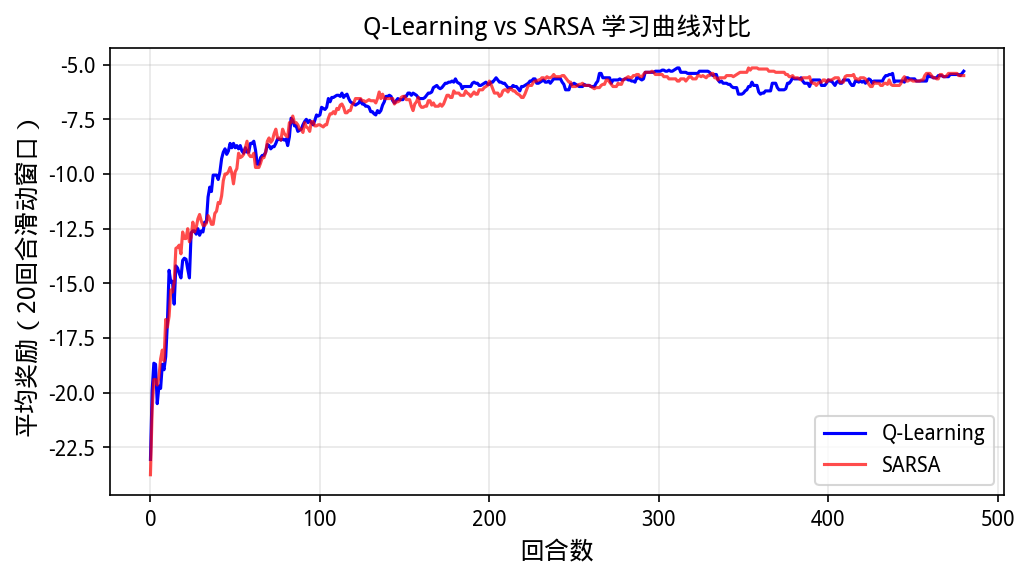
\includegraphics[width=\textwidth]{figs/chap10_qlearning_sarsa.png}
\end{minipage}
\hfill
\begin{minipage}{0.42\textwidth}
    \centering
    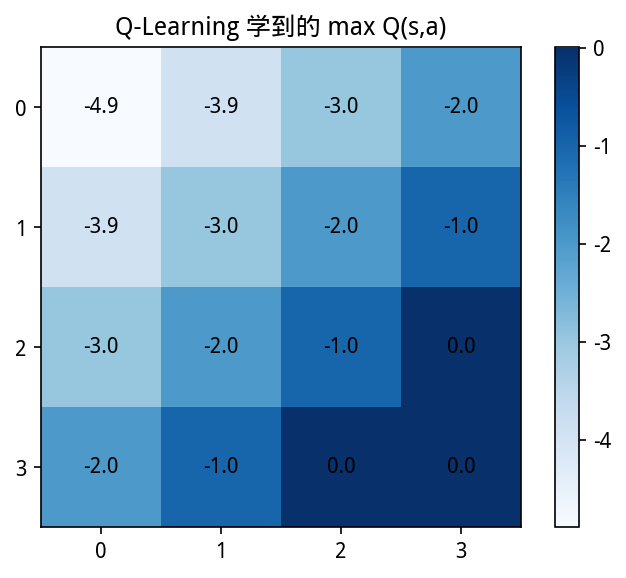
\includegraphics[width=\textwidth]{figs/chap10_qtable.png}
\end{minipage}
\caption{\textbf{左}：Q-Learning与SARSA的学习曲线对比。两种无模型算法通过与环境交互不断改进，最终都能学到接近最优的策略。\textbf{右}：Q-Learning学到的$\max_a Q(s,a)$热力图，可与图\ref{fig:value_iteration}中的值函数对比——虽然训练方式完全不同（无模型vs有模型），最终学到的值函数非常接近。}
\label{fig:qlearning_results}
\end{figure}

% ------------------------------------------------------------------------------------
\section{本章小结}
% ------------------------------------------------------------------------------------

让我们回顾这一章的核心内容：

\begin{enumerate}
    \item \textbf{贝尔曼方程的来源}：它不是凭空定义的，而是强化学习约束优化问题的KKT条件。值函数$V(s)$正是动力学约束的拉格朗日乘子。
    
    \item \textbf{最短路的启示}：通过最短路问题，我们看到了原始-对偶结构。Dijkstra代表"对偶上升"（维护最优性），Bellman-Ford代表"原始改进"（维护可行性）。
    
    \item \textbf{两个核心维度}：
    \begin{itemize}
        \item 模型可获取性：有模型（可以脑中模拟）vs 无模型（只能真实交互）
        \item 决策深度：浅（用估计值，低方差高偏差）vs 深（用真实回报，高方差低偏差）
    \end{itemize}
    
    \item \textbf{算法图谱}：动态规划、MCTS、蒙特卡洛、时序差分四大流派，以及它们的现代变体（PPO、GRPO等）。
\end{enumerate}

\begin{physicalmeaning}
强化学习的本质是：在\textbf{动力学约束}下，通过\textbf{试错与估计}找到最优决策。

不同算法的区别在于两个权衡：
\begin{itemize}
    \item 你知道多少规则？（模型）——决定能否"想象"而不必"实践"
    \item 你愿意看多远？（深度）——决定偏差与方差的取舍
\end{itemize}

从RLHF到GRPO，大语言模型对齐的最新进展告诉我们：当绝对的"奖励"难以定义时，"相对比较"（组内排序）是一条可行之路——这正是"原始改进"思想的现代演绎。
\end{physicalmeaning}

% ------------------------------------------------------------------------------------
\section{习题}
% ------------------------------------------------------------------------------------

\paragraph{概念理解}
\begin{enumerate}
    \item 用你自己的话解释：为什么说"值函数是拉格朗日乘子"？
    
    \item Dijkstra算法为什么不能处理负权边？用"对偶上升"的视角解释。
    
    \item TD学习的偏差来自哪里？在什么情况下这个偏差会特别严重？
    
    \item GRPO为什么不需要单独训练奖励模型？它和RLHF有什么本质区别？
\end{enumerate}

\paragraph{数学推导}
\begin{enumerate}
    \setcounter{enumi}{4}
    \item 写出最短路问题的原始LP和对偶LP，验证强对偶性成立。
    
    \item 证明：当$\gamma < 1$时，贝尔曼算子$T$是压缩映射，即
    \[
        \|TV_1 - TV_2\|_\infty \leq \gamma \|V_1 - V_2\|_\infty
    \]
    （提示：利用$|\max f - \max g| \leq \max |f - g|$）
\end{enumerate}

\paragraph{编程实践}
\begin{enumerate}
    \setcounter{enumi}{6}
    \item 修改GridWorld代码，添加一个"陷阱"格子（奖励$-10$）。观察值函数如何变化。
    
    \item 实现TD($\lambda$)算法，在GridWorld上比较$\lambda = 0, 0.5, 1$的学习曲线。
    
    \item （挑战）实现一个简化版的GRPO：对同一个状态采样多个动作，用组内排序来更新策略。
\end{enumerate}

\section{扩展阅读：从表格到神经网络}
% ------------------------------------------------------------------------------------

\marginnote{\textbf{Sutton与Barto}：Richard Sutton和Andrew Barto是强化学习领域的``教父''。他们1998年合著的《Reinforcement Learning: An Introduction》是该领域的圣经，免费在线阅读。Sutton提出了TD学习、策略梯度等核心算法，2024年获图灵奖提名。}

在前面的 GridWorld 例子中，我们用一个 $5 \times 5 \times 4$ 的数组来存储 $Q(s, a)$。这在状态空间很小的时候完全可行，但如果状态是一张 $84 \times 84$ 的游戏画面呢？

可能的状态数 $\approx 256^{84 \times 84} \approx 10^{17000}$

这个数字比宇宙中的原子数还要多得多。我们不可能为每个状态都存一个 $Q$ 值。

解决方案很自然：用\textbf{神经网络}来近似 $Q(s, a)$ 或 $\pi(a|s)$。这就是\textbf{深度强化学习}（Deep RL）的核心思想。

\begin{insightbox}
\textbf{为什么现代AI都围绕矩阵运算发展？}

你可能注意到了一个规律：从第3章的梯度计算，到第9章的反向传播，再到本章的强化学习，所有算法的核心都是\textbf{矩阵运算}。这不是巧合：

\begin{enumerate}
    \item \textbf{数学统一性}：神经网络的前向传播就是一系列矩阵乘法 $\bm{y} = \bm{W}\bm{x} + \bm{b}$；反向传播也是矩阵乘法的链式法则
    \item \textbf{硬件适配}：GPU 天生擅长并行矩阵运算，一块 A100 GPU 可以每秒完成 $10^{15}$ 次浮点矩阵运算
    \item \textbf{批量处理}：把 64 个样本打包成一个矩阵，一次前向传播就能处理所有样本
\end{enumerate}

所以，\textbf{理解矩阵运算 = 理解现代AI的计算基础}。这也是为什么我们在第2-3章花大量篇幅讲线性代数和矩阵求导。
\end{insightbox}

\begin{figure}[h]
\centering
\begin{tikzpicture}[>=stealth, scale=0.9]
    % 表格方法
    \begin{scope}[xshift=-5cm]
        \node[font=\bfseries] at (0, 3) {表格方法};
        
        % 表格
        \draw (0,0) grid[step=0.6] (1.8, 1.8);
        \foreach \i in {0,1,2} {
            \foreach \j in {0,1,2} {
                \node[font=\tiny] at (0.3+0.6*\i, 0.3+0.6*\j) {$Q$};
            }
        }
        
        \node[below, font=\small] at (0.9, -0.3) {每个格子存一个值};
        
        \draw[->, thick] (0, -1) -- (0, -1.8) node[below, font=\small, align=center] {状态数爆炸\\无法存储};
    \end{scope}
    
    % 箭头
    \draw[->, very thick] (-2, 1) -- (0, 1) node[midway, above, font=\small] {深度学习};
    
    % 神经网络方法
    \begin{scope}[xshift=3cm]
        \node[font=\bfseries] at (1.5, 3) {函数近似};
        
        % 输入
        \node[draw, rounded corners, fill=blue!20, minimum width=1.2cm, minimum height=1.5cm] (input) at (0, 1) {\small 状态 $s$};
        
        % 神经网络
        \node[draw, rounded corners, fill=orange!20, minimum width=1.5cm, minimum height=1.8cm, align=center] (nn) at (2.2, 1) {\small 神经\\网络};
        
        % 输出
        \node[draw, rounded corners, fill=green!20, minimum width=1.2cm, minimum height=1.5cm] (output) at (4.4, 1) {\small $Q(s,\cdot)$};
        
        \draw[->, thick] (input) -- (nn);
        \draw[->, thick] (nn) -- (output);
        
        \node[below, font=\small, align=center] at (2.2, -0.5) {网络参数 $\theta$\\可以泛化到未见过的状态};
    \end{scope}
\end{tikzpicture}
\caption{从表格方法到函数近似：神经网络用有限的参数表示无限状态空间上的值函数}
\end{figure}

% ------------------------------------------------------------------------------------
\subsection{Stable Baselines3：工业级深度强化学习库}
% ------------------------------------------------------------------------------------

\href{https://stable-baselines3.readthedocs.io/}{Stable Baselines3}（简称 SB3）是目前最流行的深度强化学习库。它实现了 DQN、PPO、SAC 等主流算法，代码清晰、文档完善，非常适合学习。

\begin{lstlisting}[language=Python, caption={用 SB3 训练一个 PPO 智能体}]
from stable_baselines3 import PPO
import gymnasium as gym

# 创建环境
env = gym.make("CartPole-v1")

# 创建智能体（一行代码！）
model = PPO("MlpPolicy", env, verbose=1)

# 训练
model.learn(total_timesteps=10000)

# 测试
obs, _ = env.reset()
for _ in range(1000):
    action, _ = model.predict(obs)
    obs, reward, done, _, _ = env.step(action)
    if done:
        obs, _ = env.reset()
\end{lstlisting}

看起来很简单，但背后隐藏着大量的工程细节。让我们深入源代码，看看这些算法到底是怎么实现的。

% ------------------------------------------------------------------------------------
\subsection{DQN：从 Q-Learning 到深度网络}
% ------------------------------------------------------------------------------------

\marginnote{\textbf{DeepMind与DQN}：2013年，伦敦创业公司DeepMind（由Demis Hassabis、Shane Legg等创立）在arXiv发布DQN论文，用神经网络玩Atari游戏达到人类水平。2014年Google以约6亿美元收购DeepMind。2015年DQN正式发表于Nature，开启深度强化学习时代。两年后AlphaGo击败世界围棋冠军，震惊世界。}

\marginnote{\textbf{Demis Hassabis}(1976--)：DeepMind联合创始人兼CEO，2024年诺贝尔化学奖得主（因AlphaFold蛋白质结构预测）。他是国际象棋神童，13岁时已是世界第二年轻的大师。他先后在剑桥和UCL获得学位，是少数同时在AI和神经科学两个领域做出重要贡献的人。}

DQN 是深度强化学习的开山之作（Mnih et al., 2015）。它的核心思想是用神经网络代替 Q 表格，但这带来了两个新问题：

\begin{enumerate}
    \item \textbf{数据相关性}：连续的游戏帧高度相关，直接训练会导致网络"过拟合"到最近的经验
    \item \textbf{目标不稳定}：TD 目标 $r + \gamma \max_{a'} Q(s', a')$ 依赖于 $Q$ 网络本身，形成"追逐移动靶心"
\end{enumerate}

DQN 的两个关键技巧正是为了解决这两个问题：

\begin{figure}[h]
\centering
\begin{tikzpicture}[>=stealth, scale=0.85]
    % 经验回放
    \begin{scope}[xshift=-4.5cm]
        \node[font=\bfseries] at (0, 3.5) {技巧一：经验回放};
        
        % 经验池
        \node[draw, rounded corners, fill=yellow!20, minimum width=3cm, minimum height=2cm] (buffer) at (0, 1.5) {};
        \node at (0, 2.2) {\small 经验池};
        
        % 经验条目
        \node[font=\tiny] at (0, 1.8) {$(s_1, a_1, r_1, s_1')$};
        \node[font=\tiny] at (0, 1.4) {$(s_2, a_2, r_2, s_2')$};
        \node[font=\tiny] at (0, 1.0) {$\vdots$};
        
        % 随机采样
        \draw[->, thick] (0, 0.3) -- (0, -0.5) node[below, font=\small, align=center] {随机采样\\打破相关性};
    \end{scope}
    
    % 目标网络
    \begin{scope}[xshift=3.5cm]
        \node[font=\bfseries] at (0, 3.5) {技巧二：目标网络};
        
        % 当前网络
        \node[draw, rounded corners, fill=blue!20, minimum width=2cm, minimum height=1cm] (q) at (-1.2, 2) {\small $Q_\theta$};
        \node[below, font=\tiny] at (-1.2, 1.4) {每步更新};
        
        % 目标网络
        \node[draw, rounded corners, fill=green!20, minimum width=2cm, minimum height=1cm] (qt) at (1.2, 2) {\small $Q_{\theta^-}$};
        \node[below, font=\tiny] at (1.2, 1.4) {定期复制};
        
        % 箭头
        \draw[->, thick, dashed] (q) -- node[above, font=\tiny] {周期性} (qt);
        
        % 说明
        \node[below, font=\small, align=center] at (0, 0) {用 $Q_{\theta^-}$ 计算目标\\稳定训练过程};
    \end{scope}
\end{tikzpicture}
\caption{DQN 的两个核心技巧}
\end{figure}

以下是 DQN 的核心训练逻辑（简化自 SB3 源码）。

\begin{insightbox}
\textbf{代码说明}：本节的 DQN、PPO、SAC 代码是\textbf{算法结构概览}，用于帮助理解核心逻辑。完整可运行的代码见 \texttt{code/chap10\_rl.py}（值迭代、Q-Learning、SARSA）和 Stable-Baselines3 库。

\textbf{为什么这里用概览代码？} 真实的 DQN/PPO 实现涉及大量工程细节（网络定义、数据加载、日志记录等），会淹没核心算法思想。我们先理解"骨架"，再去看完整实现。
\end{insightbox}

\begin{lstlisting}[language=Python, caption={DQN 核心算法（算法概览）}]
class DQN:
    def __init__(self, env):
        self.q_network = NeuralNetwork()        # Q 网络
        self.target_network = copy(self.q_network)  # 目标网络
        self.buffer = ReplayBuffer(size=100000)  # 经验池
        self.gamma = 0.99
        self.epsilon = 0.1  # 探索率
        
    def select_action(self, state):
        """epsilon-贪婪策略"""
        if random() < self.epsilon:
            return env.action_space.sample()  # 随机探索
        else:
            q_values = self.q_network(state)
            return argmax(q_values)  # 选最优
    
    def train_step(self, batch_size=64):
        """一步训练"""
        # 1. 从经验池随机采样
        states, actions, rewards, next_states, dones = \
            self.buffer.sample(batch_size)
        
        # 2. 计算 TD 目标（用目标网络！）
        with torch.no_grad():
            next_q_values = self.target_network(next_states)
            max_next_q = next_q_values.max(dim=1)
            td_target = rewards + self.gamma * max_next_q * (1 - dones)
        
        # 3. 计算当前 Q 值
        current_q = self.q_network(states)
        current_q = current_q.gather(1, actions)  # 选出执行动作的Q值
        
        # 4. 计算损失并更新（这就是 Bellman 误差！）
        loss = F.mse_loss(current_q, td_target)
        
        self.optimizer.zero_grad()
        loss.backward()
        self.optimizer.step()
        
    def update_target_network(self):
        """定期更新目标网络"""
        self.target_network.load_state_dict(
            self.q_network.state_dict()
        )
\end{lstlisting}

\begin{keyidea}[DQN 的损失函数就是 Bellman 误差]
\begin{equation}
    \mathcal{L}(\theta) = \mathbb{E}_{(s,a,r,s') \sim \mathcal{D}} \left[ \left( Q_\theta(s, a) - \underbrace{\left( r + \gamma \max_{a'} Q_{\theta^-}(s', a') \right)}_{\text{TD 目标（用目标网络）}} \right)^2 \right]
\end{equation}
这正是让 Bellman 方程"左边等于右边"的 L2 损失！
\end{keyidea}

% ------------------------------------------------------------------------------------
\subsection{PPO：稳健的策略梯度}
% ------------------------------------------------------------------------------------

\marginnote{\textbf{PPO与OpenAI}：PPO由OpenAI的John Schulman等人于2017年提出。Schulman此前还提出了TRPO（2015），但TRPO计算复杂。PPO通过简单的``裁剪''技巧获得类似效果，实现简单、调参容易，成为工业界标配。2022年ChatGPT的RLHF训练正是使用PPO，让AI学会遵循人类偏好。}

PPO（Proximal Policy Optimization）是目前工业界最常用的算法，ChatGPT 的 RLHF 训练就用的它。

与 DQN 不同，PPO 不是去拟合 Bellman 方程，而是\textbf{直接优化策略}。它的目标很直接：让好动作的概率变高，坏动作的概率变低。

\begin{figure}[h]
\centering
\begin{tikzpicture}[>=stealth, scale=0.9]
    % Actor-Critic 结构
    \node[draw, rounded corners, fill=blue!20, minimum width=2cm, minimum height=1.2cm] (state) at (0, 0) {状态 $s$};
    
    \node[draw, rounded corners, fill=orange!20, minimum width=2.5cm, minimum height=1.2cm] (actor) at (4, 1) {Actor $\pi_\theta$};
    \node[draw, rounded corners, fill=green!20, minimum width=2.5cm, minimum height=1.2cm] (critic) at (4, -1) {Critic $V_\phi$};
    
    \node[draw, rounded corners, fill=red!10, minimum width=2cm, minimum height=0.8cm] (action) at (8, 1) {动作 $a$};
    \node[draw, rounded corners, fill=purple!10, minimum width=2cm, minimum height=0.8cm] (value) at (8, -1) {价值 $V(s)$};
    
    \draw[->, thick] (state) -- (actor);
    \draw[->, thick] (state) -- (critic);
    \draw[->, thick] (actor) -- (action);
    \draw[->, thick] (critic) -- (value);
    
    \node[below, font=\small, gray] at (4, 1.8) {输出动作分布};
    \node[below, font=\small, gray] at (4, -0.2) {估计状态价值};
\end{tikzpicture}
\caption{PPO 的 Actor-Critic 结构：Actor 决定做什么，Critic 评估好不好}
\end{figure}

PPO 的核心创新是\textbf{Clip 机制}——限制每次更新的幅度，防止策略变化太大导致训练崩溃。

\begin{lstlisting}[language=Python, caption={PPO 核心算法}]
class PPO:
    def __init__(self, env):
        self.actor = PolicyNetwork()   # 策略网络 pi(a|s)
        self.critic = ValueNetwork()   # 价值网络 V(s)
        self.gamma = 0.99
        self.gae_lambda = 0.95  # GAE 参数
        self.clip_range = 0.2   # PPO 的核心：裁剪范围
        
    def collect_rollout(self, n_steps):
        """收集一段轨迹（On-policy：必须用当前策略！）"""
        trajectory = []
        state = self.env.reset()
        
        for _ in range(n_steps):
            with torch.no_grad():
                # Actor 输出动作分布，采样一个动作
                action_dist = self.actor(state)
                action = action_dist.sample()
                log_prob = action_dist.log_prob(action)
                value = self.critic(state)
            
            next_state, reward, done = self.env.step(action)
            trajectory.append({
                'state': state,
                'action': action,
                'log_prob': log_prob,  # 记住旧策略的概率
                'value': value,
                'reward': reward,
                'done': done
            })
            state = next_state
            
        return trajectory
    
    def compute_gae(self, trajectory):
        """计算广义优势估计（GAE）"""
        advantages = []
        gae = 0
        
        # 从后往前计算
        for t in reversed(range(len(trajectory))):
            if t == len(trajectory) - 1:
                next_value = 0
            else:
                next_value = trajectory[t+1]['value']
            
            # TD 误差
            delta = trajectory[t]['reward'] + \
                    self.gamma * next_value * (1 - trajectory[t]['done']) - \
                    trajectory[t]['value']
            
            # GAE 递推
            gae = delta + self.gamma * self.gae_lambda * gae
            advantages.insert(0, gae)
            
        return advantages
    
    def train(self, trajectory, advantages):
        """PPO 更新（可以用同一批数据更新多次！）"""
        
        # 计算回报（用于训练 Critic）
        returns = [adv + traj['value'] 
                   for adv, traj in zip(advantages, trajectory)]
        
        # 多个 epoch 更新（数据复用，但有 clip 保护）
        for epoch in range(K_EPOCHS):
            for batch in make_batches(trajectory):
                # --- Actor 损失：PPO-Clip ---
                
                # 新策略下的 log 概率
                new_dist = self.actor(batch['states'])
                new_log_prob = new_dist.log_prob(batch['actions'])
                
                # 概率比率 r(theta) = pi_new / pi_old
                ratio = torch.exp(new_log_prob - batch['old_log_probs'])
                
                # PPO 核心：裁剪目标
                surr1 = ratio * batch['advantages']
                surr2 = torch.clamp(ratio, 
                                    1 - self.clip_range,
                                    1 + self.clip_range) * batch['advantages']
                actor_loss = -torch.min(surr1, surr2).mean()
                
                # --- Critic 损失：简单的 MSE ---
                value_pred = self.critic(batch['states'])
                critic_loss = F.mse_loss(value_pred, batch['returns'])
                
                # --- 总损失 ---
                loss = actor_loss + 0.5 * critic_loss
                
                self.optimizer.zero_grad()
                loss.backward()
                self.optimizer.step()
        
        # On-policy：用完就丢！
        trajectory.clear()
\end{lstlisting}

\begin{keyidea}[PPO 的 Clip 机制]
\begin{equation}
    \mathcal{L}^{CLIP}(\theta) = \mathbb{E}_t \left[ \min \left( r_t(\theta) A_t, \; \text{clip}(r_t(\theta), 1-\epsilon, 1+\epsilon) A_t \right) \right]
\end{equation}
其中 $r_t(\theta) = \frac{\pi_\theta(a_t|s_t)}{\pi_{\theta_{old}}(a_t|s_t)}$ 是新旧策略的概率比。

当 $A_t > 0$（好动作）时，我们想增加 $r_t$，但最多增加到 $1+\epsilon$；\\
当 $A_t < 0$（坏动作）时，我们想减少 $r_t$，但最多减少到 $1-\epsilon$。

这样就防止了策略更新"步子迈太大"。
\end{keyidea}

% ------------------------------------------------------------------------------------
\subsection{SAC：最大熵强化学习}
% ------------------------------------------------------------------------------------

\marginnote{\textbf{SAC与Berkeley}：SAC由UC Berkeley的Tuomas Haarnoja等人于2018年提出，导师是Pieter Abbeel和Sergey Levine——两位机器人强化学习的领军人物。SAC的``最大熵''思想来自信息论，让策略保持适度随机性以增强探索和鲁棒性，在机器人操作任务中表现出色。}

SAC（Soft Actor-Critic）是连续控制任务的首选算法，在机器人控制领域表现优异。

SAC 的核心思想是：不仅要最大化奖励，还要最大化策略的\textbf{熵}（随机性）。这听起来很奇怪——我们不是应该找到最优动作然后一直执行吗？

\begin{figure}[h]
\centering
\begin{tikzpicture}[>=stealth, scale=0.9]
    % 普通 RL
    \begin{scope}[xshift=-4cm]
        \node[font=\bfseries] at (0, 3.5) {普通 RL};
        
        \draw[->] (-1.5, 0) -- (1.5, 0) node[right] {$a$};
        \draw[->] (0, 0) -- (0, 2) node[above] {$\pi(a|s)$};
        
        % 尖峰分布
        \draw[thick, blue, fill=blue!20] (-0.1, 0) -- (0, 1.8) -- (0.1, 0) -- cycle;
        
        \node[below, font=\small] at (0, -0.5) {确定性策略};
        \node[below, font=\tiny, gray] at (0, -1) {容易陷入局部最优};
    \end{scope}
    
    % SAC
    \begin{scope}[xshift=4cm]
        \node[font=\bfseries] at (0, 3.5) {SAC（最大熵）};
        
        \draw[->] (-1.5, 0) -- (1.5, 0) node[right] {$a$};
        \draw[->] (0, 0) -- (0, 2) node[above] {$\pi(a|s)$};
        
        % 高斯分布
        \draw[thick, red, fill=red!20, domain=-1.3:1.3, samples=50] 
            plot (\x, {1.5*exp(-2*\x*\x)});
        
        \node[below, font=\small] at (0, -0.5) {随机策略};
        \node[below, font=\tiny, gray] at (0, -1) {保持探索，更鲁棒};
    \end{scope}
\end{tikzpicture}
\caption{普通 RL 学出尖锐的确定性策略，SAC 保持策略的随机性}
\end{figure}

为什么要保持随机性？
\begin{itemize}
    \item \textbf{更好的探索}：随机策略能发现更多可能性
    \item \textbf{更强的鲁棒性}：面对扰动时不会彻底崩溃
    \item \textbf{避免局部最优}：不会过早锁死在某个策略上
\end{itemize}

\begin{lstlisting}[language=Python, caption={SAC 核心算法}]
class SAC:
    def __init__(self, env):
        # SAC 有 5 个网络！
        self.actor = GaussianPolicy()     # 输出动作的均值和方差
        self.critic_1 = QNetwork()        # Q1(s, a)
        self.critic_2 = QNetwork()        # Q2(s, a) - 双Q减少过估计
        self.target_critic_1 = copy(self.critic_1)
        self.target_critic_2 = copy(self.critic_2)
        
        self.alpha = 0.2  # 熵系数（温度）
        self.buffer = ReplayBuffer()
        
    def select_action(self, state):
        """从高斯分布采样动作"""
        mean, std = self.actor(state)
        dist = Normal(mean, std)
        action = dist.rsample()  # 重参数化采样（可导！）
        return torch.tanh(action)  # 压缩到 [-1, 1]
    
    def train_step(self, batch_size=256):
        batch = self.buffer.sample(batch_size)
        
        # --- 更新 Critic ---
        with torch.no_grad():
            # 用当前策略采样下一个动作
            next_action, next_log_prob = self.actor.sample(
                batch['next_states']
            )
            
            # 双Q网络：取较小的那个（悲观估计）
            target_q1 = self.target_critic_1(
                batch['next_states'], next_action
            )
            target_q2 = self.target_critic_2(
                batch['next_states'], next_action
            )
            target_q = torch.min(target_q1, target_q2)
            
            # SAC 的目标：Q - alpha * log_prob（软Q值）
            target = batch['rewards'] + self.gamma * (
                target_q - self.alpha * next_log_prob
            )
        
        # Critic 损失
        q1 = self.critic_1(batch['states'], batch['actions'])
        q2 = self.critic_2(batch['states'], batch['actions'])
        critic_loss = F.mse_loss(q1, target) + F.mse_loss(q2, target)
        
        self.critic_optimizer.zero_grad()
        critic_loss.backward()
        self.critic_optimizer.step()
        
        # --- 更新 Actor ---
        # 重参数化技巧：a = tanh(mu + sigma * epsilon)
        new_action, log_prob = self.actor.rsample(batch['states'])
        
        q_value = torch.min(
            self.critic_1(batch['states'], new_action),
            self.critic_2(batch['states'], new_action)
        )
        
        # Actor 目标：最大化 Q - alpha * log_prob
        # 等价于最小化 alpha * log_prob - Q
        actor_loss = (self.alpha * log_prob - q_value).mean()
        
        self.actor_optimizer.zero_grad()
        actor_loss.backward()
        self.actor_optimizer.step()
        
        # --- 软更新目标网络（Polyak 平均）---
        for target_param, param in zip(
            self.target_critic_1.parameters(),
            self.critic_1.parameters()
        ):
            target_param.data.copy_(
                0.995 * target_param.data + 0.005 * param.data
            )
        # target_critic_2 同理
\end{lstlisting}

\begin{keyidea}[title=SAC 的优化目标]
SAC 最大化的不是普通的累积奖励，而是带熵正则的目标：
\begin{equation}
    J(\pi) = \sum_{t=0}^{\infty} \mathbb{E}_{(s_t, a_t) \sim \pi} \left[ r(s_t, a_t) + \alpha \underbrace{\mathcal{H}(\pi(\cdot|s_t))}_{\text{策略熵}} \right]
\end{equation}
其中 $\alpha$ 是温度系数，控制"探索 vs 利用"的权衡。
\end{keyidea}

% ------------------------------------------------------------------------------------
\subsection{三种算法的对比总结}
% ------------------------------------------------------------------------------------

\begin{table}[h]
\centering
\small
\renewcommand{\arraystretch}{1.4}
\caption{DQN、PPO、SAC 的核心对比}
\begin{tabular}{p{2.2cm}|p{3.8cm}|p{3.8cm}|p{3.8cm}}
\toprule
& \textbf{DQN} & \textbf{PPO} & \textbf{SAC} \\
\midrule
\textbf{学什么} & Q 值函数 $Q(s,a)$ & 策略 $\pi(a|s)$ + 价值 $V(s)$ & 策略 $\pi(a|s)$ + Q值 $Q(s,a)$ \\
\midrule
\textbf{动作空间} & 离散 & 离散或连续 & 连续 \\
\midrule
\textbf{数据策略} & Off-policy（经验回放） & On-policy（用完即弃） & Off-policy（经验回放） \\
\midrule
\textbf{核心技巧} & 目标网络 & Clip 裁剪 & 最大熵 + 双Q网络 \\
\midrule
\textbf{损失函数} & Bellman 误差 (MSE) & Clip 策略损失 + 价值 MSE & 软 Bellman 误差 + 策略熵 \\
\midrule
\textbf{典型应用} & Atari 游戏 & ChatGPT、机器人 & 机器人控制 \\
\bottomrule
\end{tabular}
\end{table}

\begin{figure}[h]
\centering
\begin{tikzpicture}[scale=0.9]
    % 坐标轴
    \draw[->, thick] (-0.5, 0) -- (10, 0) node[right] {实现复杂度};
    \draw[->, thick] (0, -0.5) -- (0, 5) node[above] {样本效率};
    
    % 算法位置
    \node[draw, circle, fill=blue!30, minimum size=1.2cm] (dqn) at (2, 2) {DQN};
    \node[draw, circle, fill=orange!30, minimum size=1.2cm] (ppo) at (5, 3) {PPO};
    \node[draw, circle, fill=green!30, minimum size=1.2cm] (sac) at (8, 4.5) {SAC};
    
    % 标注
    \node[below, font=\small] at (2, 1.2) {简单、入门};
    \node[below, font=\small] at (5, 2.2) {稳健、通用};
    \node[below, font=\small] at (8, 3.7) {高效、复杂};
    
    % 箭头表示演进
    \draw[->, dashed, gray] (dqn) -- (ppo);
    \draw[->, dashed, gray] (ppo) -- (sac);
\end{tikzpicture}
\caption{三种算法的定位：从简单到复杂，从低效到高效}
\end{figure}

% ------------------------------------------------------------------------------------
\subsection{动手实践：用 SB3 训练经典控制任务}
% ------------------------------------------------------------------------------------

以下代码展示如何用 SB3 在经典控制任务上训练和对比三种算法：

\begin{lstlisting}[language=Python, caption={用 SB3 对比三种算法}]
import gymnasium as gym
from stable_baselines3 import DQN, PPO, SAC
import matplotlib.pyplot as plt

# CartPole: 离散动作，适合 DQN 和 PPO
env_discrete = gym.make("CartPole-v1")

# Pendulum: 连续动作，适合 PPO 和 SAC
env_continuous = gym.make("Pendulum-v1")

# --- 训练 DQN（离散动作）---
dqn_model = DQN(
    "MlpPolicy", 
    env_discrete,
    learning_rate=1e-3,
    buffer_size=50000,      # 经验池大小
    learning_starts=1000,   # 开始训练前先收集多少数据
    target_update_interval=500,  # 目标网络更新频率
    verbose=1
)
dqn_model.learn(total_timesteps=20000)

# --- 训练 PPO（通用）---
ppo_model = PPO(
    "MlpPolicy",
    env_discrete,
    learning_rate=3e-4,
    n_steps=2048,           # 每次收集多少步
    batch_size=64,          # 小批量大小
    n_epochs=10,            # 每批数据训练几轮
    clip_range=0.2,         # PPO clip 参数
    verbose=1
)
ppo_model.learn(total_timesteps=20000)

# --- 训练 SAC（连续动作）---
sac_model = SAC(
    "MlpPolicy",
    env_continuous,
    learning_rate=3e-4,
    buffer_size=100000,
    learning_starts=1000,
    tau=0.005,              # 软更新系数
    verbose=1
)
sac_model.learn(total_timesteps=20000)
\end{lstlisting}

\begin{remark}
SB3 的强大之处在于：\textbf{把这里的 \texttt{CartPole} 换成你的自定义环境，代码几乎不用改}。

只要你的问题能封装成 Gymnasium 接口：
\begin{itemize}
    \item \texttt{reset()} 返回初始状态
    \item \texttt{step(action)} 返回 (下一状态, 奖励, 是否结束, 信息)
\end{itemize}

那么 SB3 就能直接训练。把 CartPole 的物理方程换成飞行器动力学，就是飞行控制；换成流体方程，就是流体控制。
\end{remark}




\section{扩展阅读：深度强化学习与约束优化的深层联系}
% ------------------------------------------------------------------------------------

在第一章中，我们用拉格朗日乘子法推导出了贝尔曼方程。现在让我们反过来思考：既然强化学习本质上是一个约束优化问题，那么现代算法（如 PPO）是如何处理这些约束的？

这一节我们将揭示 PPO 背后的优化理论，以及从 TRPO 到 PPO 的演化过程中，研究者是如何用工程技巧来近似复杂的约束优化的。

% ------------------------------------------------------------------------------------
\subsection{策略优化的本质困难}
% ------------------------------------------------------------------------------------

假设我们想直接优化策略 $\pi_\theta$，最大化累积奖励：
\begin{equation}
    \max_\theta \; J(\theta) = \mathbb{E}_{\tau \sim \pi_\theta} \left[ \sum_{t=0}^{T} \gamma^t r_t \right]
\end{equation}

这看起来就是一个普通的优化问题，用梯度上升不就行了吗？

\begin{equation}
    \theta \leftarrow \theta + \alpha \nabla_\theta J(\theta)
\end{equation}

问题在于：\textbf{策略梯度的方差极大，而且步长很难选择}。

\begin{figure}[h]
\centering
\begin{tikzpicture}[>=stealth, scale=0.9]
    % 损失曲面
    \draw[thick, domain=-3:3, samples=100, blue] 
        plot (\x, {0.3*\x*\x - 0.5*cos(3*\x r) + 2});
    
    % 当前位置
    \fill[red] (-1.5, 2.175) circle (3pt);
    \node[above right, font=\small] at (-1.5, 2.175) {当前策略 $\theta$};
    
    % 小步长
    \draw[->, thick, green!60!black] (-1.5, 2.175) -- (-0.8, 1.8);
    \node[below, font=\scriptsize, green!60!black] at (-1.15, 1.8) {小步长：安全但慢};
    
    % 大步长（跳过去）
    \draw[->, thick, red, dashed] (-1.5, 2.175) -- (1.5, 2.5);
    \node[above, font=\scriptsize, red] at (0, 2.8) {大步长：可能跳到很差的地方};
    
    % 悬崖
    \fill[red!20] (0.8, 0) rectangle (1.2, 3.5);
    \node[font=\scriptsize, red] at (1, 3.8) {性能悬崖};
    
    \draw[->] (-3.5, 0) -- (3.5, 0) node[right] {$\theta$};
    \draw[->] (-3, -0.5) -- (-3, 4) node[above] {$-J(\theta)$};
\end{tikzpicture}
\caption{策略优化的困难：损失曲面高度非凸，步长太大可能跳入"性能悬崖"}
\end{figure}

更糟糕的是，策略的微小变化可能导致\textbf{采样分布的巨大变化}。想象一下：

\begin{itemize}
    \item 旧策略 $\pi_{old}$：在状态 $s$ 有 90\% 概率选动作 $a_1$
    \item 新策略 $\pi_{new}$：在状态 $s$ 有 90\% 概率选动作 $a_2$
\end{itemize}

虽然参数 $\theta$ 可能只变了一点点，但智能体的行为完全不同了！这就是为什么普通的梯度下降在策略优化中经常失败。

% ------------------------------------------------------------------------------------
\subsection{信任域方法：把优化问题变成约束优化}
% ------------------------------------------------------------------------------------

解决方案是：\textbf{限制每次更新的幅度}。

这正是\textbf{信任域方法}（Trust Region Methods）的核心思想。我们不是在整个参数空间里找最优，而是在当前点附近的一个"信任域"里找最优。

\begin{keyidea}[信任域优化]
每一步解决以下约束优化问题：
\begin{equation}
    \begin{aligned}
        \max_\theta \quad & L(\theta) = \mathbb{E}_{s,a \sim \pi_{old}} \left[ \frac{\pi_\theta(a|s)}{\pi_{old}(a|s)} A^{\pi_{old}}(s,a) \right] \\
        \text{s.t.} \quad & D(\pi_\theta, \pi_{old}) \leq \delta
    \end{aligned}
\end{equation}
其中 $D$ 是某种"距离"度量，$\delta$ 是信任域半径。
\end{keyidea}

这里的 $L(\theta)$ 叫做\textbf{替代目标}（Surrogate Objective）。它的含义是：

\begin{itemize}
    \item $\frac{\pi_\theta(a|s)}{\pi_{old}(a|s)}$：新旧策略的概率比
    \item $A^{\pi_{old}}(s,a)$：在旧策略下，动作 $a$ 比平均水平好多少（优势函数）
    \item 整体意义：如果 $A > 0$（好动作），增大概率比；如果 $A < 0$（坏动作），减小概率比
\end{itemize}

% ------------------------------------------------------------------------------------
\subsection{TRPO：用拉格朗日对偶求解}
% ------------------------------------------------------------------------------------

TRPO（Trust Region Policy Optimization）选择 KL 散度作为距离度量：

\begin{equation}
    \begin{aligned}
        \max_\theta \quad & L(\theta) \\
        \text{s.t.} \quad & \bar{D}_{KL}(\pi_{old} \| \pi_\theta) \leq \delta
    \end{aligned}
\end{equation}

其中 $\bar{D}_{KL}$ 是对所有状态取平均的 KL 散度。

\paragraph{拉格朗日对偶}

这是一个不等式约束优化问题，自然想到用拉格朗日乘子法：

\begin{equation}
    \mathcal{L}(\theta, \lambda) = L(\theta) - \lambda \left( \bar{D}_{KL}(\pi_{old} \| \pi_\theta) - \delta \right)
\end{equation}

对偶问题是：
\begin{equation}
    \min_{\lambda \geq 0} \max_\theta \mathcal{L}(\theta, \lambda)
\end{equation}

\paragraph{二阶近似与自然梯度}

TRPO 的关键洞察是：在 $\theta_{old}$ 附近，可以用泰勒展开近似：

\begin{align}
    L(\theta) &\approx L(\theta_{old}) + g^T (\theta - \theta_{old}) \\
    \bar{D}_{KL} &\approx \frac{1}{2} (\theta - \theta_{old})^T F (\theta - \theta_{old})
\end{align}

其中 $g = \nabla_\theta L|_{\theta_{old}}$ 是策略梯度，$F$ 是\textbf{Fisher 信息矩阵}：

\begin{equation}
    F = \mathbb{E}_{s \sim \pi_{old}} \left[ \nabla_\theta \log \pi_\theta(a|s) \nabla_\theta \log \pi_\theta(a|s)^T \right]_{\theta = \theta_{old}}
\end{equation}

这样，约束优化问题变成了一个\textbf{二次规划}：

\begin{equation}
    \begin{aligned}
        \max_{\Delta\theta} \quad & g^T \Delta\theta \\
        \text{s.t.} \quad & \frac{1}{2} \Delta\theta^T F \Delta\theta \leq \delta
    \end{aligned}
\end{equation}

用 KKT 条件可以得到解析解：

\begin{equation}
    \Delta\theta^* = \sqrt{\frac{2\delta}{g^T F^{-1} g}} F^{-1} g
\end{equation}

这就是\textbf{自然梯度}（Natural Gradient）！它的方向是 $F^{-1} g$，不是普通梯度 $g$。

\begin{figure}[h]
\centering
\begin{tikzpicture}[>=stealth, scale=1.0]
    % 椭圆等高线（KL 约束）
    \draw[thick, blue, rotate=30] (0,0) ellipse (2 and 1);
    \draw[thick, blue!60, rotate=30] (0,0) ellipse (1.5 and 0.75);
    \draw[thick, blue!30, rotate=30] (0,0) ellipse (1 and 0.5);
    
    % 当前点
    \fill[red] (0, 0) circle (3pt);
    \node[below left, font=\small] at (0, 0) {$\theta_{old}$};
    
    % 普通梯度方向
    \draw[->, very thick, green!60!black] (0, 0) -- (1.5, 0.8);
    \node[right, font=\small, green!60!black] at (1.5, 0.8) {普通梯度 $g$};
    
    % 自然梯度方向
    \draw[->, very thick, red] (0, 0) -- (1.2, -0.3);
    \node[right, font=\small, red] at (1.2, -0.3) {自然梯度 $F^{-1}g$};
    
    % 信任域边界
    \node[blue, font=\small] at (2.2, 1.5) {KL $= \delta$};
    
    % 说明
    \node[below, font=\small, align=center] at (0, -2) {自然梯度考虑了参数空间的"形状"\\在 KL 约束下是最优方向};
\end{tikzpicture}
\caption{普通梯度 vs 自然梯度。椭圆是 KL 散度的等高线，自然梯度是在 KL 约束下的最优方向。}
\end{figure}

\paragraph{TRPO 的数值困难}

TRPO 理论很漂亮，但实现很困难：

\begin{enumerate}
    \item \textbf{Fisher 矩阵太大}：如果网络有 $n$ 个参数，$F$ 是 $n \times n$ 矩阵。对于百万参数的网络，存储和求逆都不可行。
    
    \item \textbf{需要共轭梯度法}：TRPO 用共轭梯度（CG）来近似求解 $F^{-1}g$，需要多次计算 $Fv$（Fisher-向量乘积）。
    
    \item \textbf{需要线搜索}：二阶近似可能不准，TRPO 还需要做线搜索来确保约束真的满足。
\end{enumerate}

\begin{lstlisting}[language=Python, caption={TRPO 的核心步骤（简化版）}]
def trpo_update(policy, states, actions, advantages):
    # 1. 计算策略梯度
    g = compute_policy_gradient(policy, states, actions, advantages)
    
    # 2. 用共轭梯度法求解 F^{-1} g
    def fisher_vector_product(v):
        # 计算 Fv，不需要显式构造 F
        return compute_fvp(policy, states, v)
    
    step_dir = conjugate_gradient(fisher_vector_product, g, max_iter=10)
    
    # 3. 计算步长
    shs = 0.5 * step_dir.dot(fisher_vector_product(step_dir))
    step_size = sqrt(2 * delta / shs)
    full_step = step_size * step_dir
    
    # 4. 线搜索：确保 KL 约束满足且目标提升
    for shrink in [1, 0.5, 0.25, 0.125]:
        new_params = old_params + shrink * full_step
        if kl_divergence(new_policy, old_policy) <= delta:
            if surrogate_loss(new_policy) > surrogate_loss(old_policy):
                break
    
    return new_params
\end{lstlisting}

% ------------------------------------------------------------------------------------
\subsection{PPO：用裁剪代替约束}
% ------------------------------------------------------------------------------------

PPO 的核心洞察是：\textbf{与其精确求解约束优化，不如用一个简单的裁剪来近似}。

回顾 TRPO 的目标：
\begin{equation}
    \max_\theta \; \mathbb{E} \left[ \frac{\pi_\theta(a|s)}{\pi_{old}(a|s)} A(s,a) \right] \quad \text{s.t.} \quad D_{KL} \leq \delta
\end{equation}

PPO 的想法是：与其用 KL 散度约束概率比 $r(\theta) = \frac{\pi_\theta}{\pi_{old}}$，不如\textbf{直接裁剪概率比}！

\begin{keyidea}[PPO-Clip 目标函数]
\begin{equation}
    L^{CLIP}(\theta) = \mathbb{E} \left[ \min \left( r(\theta) A, \; \text{clip}(r(\theta), 1-\epsilon, 1+\epsilon) A \right) \right]
\end{equation}
其中 $\epsilon$ 通常取 $0.1$ 或 $0.2$。
\end{keyidea}

让我们仔细理解这个公式：

\begin{figure}[h]
\centering
\begin{tikzpicture}[>=stealth, scale=0.85]
    % A > 0 的情况
    \begin{scope}[xshift=-5cm]
        \node[font=\bfseries] at (2, 4) {当 $A > 0$（好动作）};
        
        \draw[->] (0, 0) -- (4.5, 0) node[right] {$r(\theta)$};
        \draw[->] (0, -0.5) -- (0, 3.5) node[above] {目标};
        
        % 未裁剪的目标
        \draw[thick, blue, dashed] (0, 0) -- (4, 3.2);
        \node[blue, font=\scriptsize] at (3.8, 2.5) {$rA$};
        
        % 裁剪后的目标
        \draw[very thick, red] (0, 0) -- (2.4, 1.92);
        \draw[very thick, red] (2.4, 1.92) -- (4, 1.92);
        
        % 裁剪点
        \draw[dashed, gray] (2.4, 0) -- (2.4, 1.92);
        \node[below, font=\scriptsize] at (2.4, 0) {$1+\epsilon$};
        \node[below, font=\scriptsize] at (1, 0) {$1$};
        \draw[dashed, gray] (1, 0) -- (1, 0.8);
        
        \node[below, font=\small, align=center] at (2, -1) {概率比超过 $1+\epsilon$ 后\\目标不再增加};
    \end{scope}
    
    % A < 0 的情况
    \begin{scope}[xshift=4cm]
        \node[font=\bfseries] at (2, 4) {当 $A < 0$（坏动作）};
        
        \draw[->] (0, 0) -- (4.5, 0) node[right] {$r(\theta)$};
        \draw[->] (0, -2.5) -- (0, 1) node[above] {目标};
        
        % 未裁剪的目标
        \draw[thick, blue, dashed] (0, 0) -- (4, -3.2);
        \node[blue, font=\scriptsize] at (3.8, -2.5) {$rA$};
        
        % 裁剪后的目标
        \draw[very thick, red] (0, 0) -- (0.8, -0.64);
        \draw[very thick, red] (0.8, -0.64) -- (4, -0.64);
        
        % 裁剪点
        \draw[dashed, gray] (0.8, 0) -- (0.8, -0.64);
        \node[below, font=\scriptsize] at (0.8, 0) {$1-\epsilon$};
        \node[below, font=\scriptsize] at (2, 0) {$1$};
        \draw[dashed, gray] (2, 0) -- (2, -0.5);
        
        \node[below, font=\small, align=center] at (2, -3.5) {概率比低于 $1-\epsilon$ 后\\目标不再减少};
    \end{scope}
\end{tikzpicture}
\caption{PPO 裁剪机制的效果。左：对于好动作，限制概率增加的幅度。右：对于坏动作，限制概率减少的幅度。}
\end{figure}

\paragraph{为什么裁剪有效？}

\begin{itemize}
    \item 当 $A > 0$（好动作）：我们想增大 $r(\theta)$，但超过 $1+\epsilon$ 后梯度消失，防止过度增加
    \item 当 $A < 0$（坏动作）：我们想减小 $r(\theta)$，但低于 $1-\epsilon$ 后梯度消失，防止过度减少
\end{itemize}

这相当于\textbf{隐式地}限制了策略的变化幅度，而不需要显式计算 KL 散度或 Fisher 矩阵！

\paragraph{PPO vs TRPO 的数值比较}

\begin{table}[h]
\centering
\renewcommand{\arraystretch}{1.4}
\begin{tabular}{p{3cm}|p{5cm}|p{5cm}}
\toprule
& \textbf{TRPO} & \textbf{PPO} \\
\midrule
\textbf{约束方式} & 显式 KL 散度约束 & 隐式裁剪 \\
\midrule
\textbf{需要计算} & Fisher 矩阵、共轭梯度、线搜索 & 只需要普通梯度 \\
\midrule
\textbf{每次更新} & 一步精确求解 & 多个 epoch 小步迭代 \\
\midrule
\textbf{实现难度} & 高（约 500 行核心代码） & 低（约 50 行核心代码） \\
\midrule
\textbf{计算成本} & 高（每步需要多次前向/反向传播） & 低（标准梯度下降） \\
\midrule
\textbf{性能} & 理论最优 & 实践中相当甚至更好 \\
\bottomrule
\end{tabular}
\caption{TRPO vs PPO：复杂度与性能的权衡}
\end{table}

% ------------------------------------------------------------------------------------
\subsection{PPO 的完整优化流程}
% ------------------------------------------------------------------------------------

让我们详细看看 PPO 的一次完整更新：

\begin{figure}[h]
\centering
\begin{tikzpicture}[>=stealth, scale=0.85, 
    block/.style={draw, rounded corners, minimum width=2.5cm, minimum height=1cm, align=center}]
    
    % 流程图
    \node[block, fill=blue!20] (collect) at (0, 0) {收集轨迹\\$\{s, a, r, \log\pi_{old}\}$};
    \node[block, fill=green!20] (gae) at (5, 0) {计算优势\\GAE};
    \node[block, fill=orange!20] (epoch) at (10, 0) {多轮训练\\K epochs};
    \node[block, fill=red!20] (discard) at (10, -2.5) {丢弃数据\\(On-policy)};
    
    \draw[->, thick] (collect) -- (gae);
    \draw[->, thick] (gae) -- (epoch);
    \draw[->, thick] (epoch) -- (discard);
    \draw[->, thick, dashed] (discard) -- (0, -2.5) -- (collect);
    
    % epoch 内部
    \begin{scope}[xshift=10cm, yshift=-5.5cm]
        \node[font=\bfseries] at (-5, 2.5) {每个 Epoch 内部};
        
        \node[block, fill=yellow!20, minimum width=2cm] (batch) at (0, 1.5) {采样 batch};
        \node[block, fill=purple!20, minimum width=2cm] (ratio) at (0, 0) {计算 $r(\theta)$};
        \node[block, fill=cyan!20, minimum width=2cm] (clip) at (0, -1.5) {裁剪 + 损失};
        \node[block, fill=gray!20, minimum width=2cm] (grad) at (0, -3) {梯度下降};
        
        \draw[->, thick] (batch) -- (ratio);
        \draw[->, thick] (ratio) -- (clip);
        \draw[->, thick] (clip) -- (grad);
    \end{scope}
\end{tikzpicture}
\caption{PPO 的完整训练流程}
\end{figure}

\begin{lstlisting}[language=Python, caption={PPO 优化的详细实现}]
class PPOTrainer:
    def __init__(self, policy, value_net, clip_range=0.2):
        self.policy = policy          # Actor: pi(a|s)
        self.value_net = value_net    # Critic: V(s)
        self.clip_range = clip_range
        self.gamma = 0.99
        self.gae_lambda = 0.95
        self.n_epochs = 10            # 每批数据训练几轮
        self.batch_size = 64
        
    def compute_gae(self, rewards, values, dones):
        """
        广义优势估计 (Generalized Advantage Estimation)
        平衡 TD (低方差高偏差) 和 MC (高方差低偏差)
        """
        advantages = []
        gae = 0
        
        for t in reversed(range(len(rewards))):
            if t == len(rewards) - 1:
                next_value = 0
            else:
                next_value = values[t + 1]
            
            # TD 误差: delta = r + gamma * V(s') - V(s)
            delta = rewards[t] + self.gamma * next_value * (1 - dones[t]) \
                    - values[t]
            
            # GAE 递推: A_t = delta_t + (gamma * lambda) * A_{t+1}
            # lambda=0 时退化为 TD(0)
            # lambda=1 时退化为 MC
            gae = delta + self.gamma * self.gae_lambda * (1 - dones[t]) * gae
            advantages.insert(0, gae)
        
        return torch.tensor(advantages)
    
    def compute_loss(self, batch, old_log_probs, advantages, returns):
        """计算 PPO 的损失函数"""
        
        # --- Actor 损失 (PPO-Clip) ---
        
        # 当前策略的 log 概率
        new_dist = self.policy(batch['states'])
        new_log_probs = new_dist.log_prob(batch['actions'])
        
        # 概率比 r(theta) = pi_new / pi_old = exp(log_new - log_old)
        ratio = torch.exp(new_log_probs - old_log_probs)
        
        # 裁剪
        clipped_ratio = torch.clamp(ratio, 
                                    1 - self.clip_range, 
                                    1 + self.clip_range)
        
        # PPO 目标：取两者较小值（悲观估计）
        surr1 = ratio * advantages
        surr2 = clipped_ratio * advantages
        actor_loss = -torch.min(surr1, surr2).mean()
        
        # --- Critic 损失 (简单 MSE) ---
        value_pred = self.value_net(batch['states'])
        critic_loss = F.mse_loss(value_pred, returns)
        
        # --- 熵正则化（鼓励探索）---
        entropy = new_dist.entropy().mean()
        entropy_loss = -0.01 * entropy  # 负号因为我们要最大化熵
        
        # --- 总损失 ---
        total_loss = actor_loss + 0.5 * critic_loss + entropy_loss
        
        return total_loss, {
            'actor_loss': actor_loss.item(),
            'critic_loss': critic_loss.item(),
            'entropy': entropy.item(),
            'clip_fraction': ((ratio - 1).abs() > self.clip_range).float().mean().item()
        }
    
    def update(self, trajectory):
        """PPO 的一次完整更新"""
        
        # 1. 预处理轨迹数据
        states = torch.stack([t['state'] for t in trajectory])
        actions = torch.stack([t['action'] for t in trajectory])
        rewards = [t['reward'] for t in trajectory]
        dones = [t['done'] for t in trajectory]
        old_log_probs = torch.stack([t['log_prob'] for t in trajectory])
        values = torch.stack([t['value'] for t in trajectory])
        
        # 2. 计算 GAE 和回报
        advantages = self.compute_gae(rewards, values.squeeze(), dones)
        returns = advantages + values.squeeze()
        
        # 3. 归一化优势（减少方差，稳定训练）
        advantages = (advantages - advantages.mean()) / (advantages.std() + 1e-8)
        
        # 4. 多轮训练（这是 PPO 相比 TRPO 的关键：同一批数据用多次）
        dataset = TensorDataset(states, actions, old_log_probs, 
                                advantages, returns)
        dataloader = DataLoader(dataset, batch_size=self.batch_size, 
                                shuffle=True)
        
        for epoch in range(self.n_epochs):
            for batch in dataloader:
                batch_states, batch_actions, batch_old_log_probs, \
                    batch_advantages, batch_returns = batch
                
                loss, info = self.compute_loss(
                    {'states': batch_states, 'actions': batch_actions},
                    batch_old_log_probs,
                    batch_advantages,
                    batch_returns
                )
                
                self.optimizer.zero_grad()
                loss.backward()
                
                # 梯度裁剪（防止梯度爆炸）
                torch.nn.utils.clip_grad_norm_(
                    self.policy.parameters(), max_norm=0.5
                )
                torch.nn.utils.clip_grad_norm_(
                    self.value_net.parameters(), max_norm=0.5
                )
                
                self.optimizer.step()
            
            # 监控：如果 KL 散度太大，提前停止
            # （这是 PPO 的"软约束"：虽然没有显式 KL 约束，但会监控）
            approx_kl = (old_log_probs - new_log_probs).mean()
            if approx_kl > 0.02:  # 经验阈值
                print(f"Early stopping at epoch {epoch}: KL = {approx_kl:.4f}")
                break
        
        # 5. On-policy 特性：用完就丢
        return info
\end{lstlisting}

% ------------------------------------------------------------------------------------
\subsection{GAE：优势估计的偏差-方差权衡}
% ------------------------------------------------------------------------------------

PPO 中的另一个关键组件是\textbf{广义优势估计}（GAE），它本质上是 TD 和 MC 的加权组合。

回顾不同步长的优势估计：

\begin{align}
    \hat{A}^{(1)}_t &= r_t + \gamma V(s_{t+1}) - V(s_t) = \delta_t \quad &\text{(TD，低方差高偏差)} \\
    \hat{A}^{(2)}_t &= r_t + \gamma r_{t+1} + \gamma^2 V(s_{t+2}) - V(s_t) &\text{(2-step)} \\
    &\vdots \\
    \hat{A}^{(\infty)}_t &= \sum_{k=0}^{\infty} \gamma^k r_{t+k} - V(s_t) = G_t - V(s_t) \quad &\text{(MC，高方差低偏差)}
\end{align}

GAE 用指数加权把它们结合起来：

\begin{equation}
    \hat{A}^{GAE}_t = \sum_{l=0}^{\infty} (\gamma \lambda)^l \delta_{t+l}
\end{equation}

其中 $\lambda \in [0, 1]$ 控制权衡：
\begin{itemize}
    \item $\lambda = 0$：退化为 TD(0)，低方差但高偏差
    \item $\lambda = 1$：退化为 MC，高方差但无偏差
    \item $\lambda \approx 0.95$：实践中的常用值，平衡两者
\end{itemize}

\begin{figure}[h]
\centering
\begin{tikzpicture}[>=stealth, scale=0.9]
    \draw[->] (0, 0) -- (10, 0) node[right] {$\lambda$};
    \draw[->] (0, 0) -- (0, 4) node[above] {};
    
    % 偏差曲线
    \draw[thick, blue, domain=0:9.5, samples=50] 
        plot (\x, {3 * exp(-0.3*\x)});
    \node[blue, right] at (9.5, 0.5) {偏差};
    
    % 方差曲线
    \draw[thick, red, domain=0:9.5, samples=50] 
        plot (\x, {0.3 + 0.3*\x});
    \node[red, right] at (9.5, 3.3) {方差};
    
    % 最优点
    \draw[dashed, gray] (6, 0) -- (6, 2.5);
    \node[below] at (6, 0) {$\lambda^*$};
    \fill[green!60!black] (6, 1.8) circle (4pt);
    \node[above right, font=\small, green!60!black] at (6, 1.8) {平衡点};
    
    % 标注
    \node[below] at (0, 0) {$0$};
    \node[below] at (9.5, 0) {$1$};
    \node[below, font=\small] at (0, -0.8) {TD(0)};
    \node[below, font=\small] at (9.5, -0.8) {MC};
\end{tikzpicture}
\caption{GAE 的偏差-方差权衡。$\lambda$ 越大，方差越高但偏差越低。}
\end{figure}

% ------------------------------------------------------------------------------------
\subsection{数值稳定性技巧}
% ------------------------------------------------------------------------------------

在实际实现中，有很多数值稳定性的细节需要注意：

\textbf{1. 优势函数归一化}

\begin{lstlisting}[language=Python]
# 归一化优势函数，减少方差
advantages = (advantages - advantages.mean()) / (advantages.std() + 1e-8)
\end{lstlisting}

为什么有效？归一化后，优势函数大约一半是正的、一半是负的，梯度更新更平衡。

\textbf{2. 梯度裁剪}

\begin{lstlisting}[language=Python]
# 防止梯度爆炸
torch.nn.utils.clip_grad_norm_(model.parameters(), max_norm=0.5)
\end{lstlisting}

策略梯度可能突然变得很大，导致参数更新过猛。

\textbf{3. 学习率调度}

\begin{lstlisting}[language=Python]
# 线性衰减学习率
def linear_schedule(progress):
    return 1 - progress  # progress 从 0 到 1

scheduler = LambdaLR(optimizer, lr_lambda=linear_schedule)
\end{lstlisting}

训练后期降低学习率有助于稳定收敛。

\textbf{4. 价值函数裁剪（可选）}

\begin{lstlisting}[language=Python]
# 限制价值函数的更新幅度
value_clipped = old_values + torch.clamp(
    value_pred - old_values, -clip_range, clip_range
)
critic_loss = torch.max(
    (value_pred - returns)**2,
    (value_clipped - returns)**2
).mean()
\end{lstlisting}

类似于策略裁剪，防止价值函数变化太大。

% ------------------------------------------------------------------------------------
\subsection{从优化角度看不同 RL 算法}
% ------------------------------------------------------------------------------------

现在我们可以从约束优化的角度统一理解各种算法：

\begin{table}[h]
\centering
\small
\renewcommand{\arraystretch}{1.5}
\caption{从约束优化角度看 RL 算法}
\begin{tabular}{p{2cm}|p{3.5cm}|p{4cm}|p{4cm}}
\toprule
\textbf{算法} & \textbf{优化目标} & \textbf{约束/正则} & \textbf{求解方法} \\
\midrule
\textbf{DQN} & Bellman 误差 & 目标网络（隐式稳定） & 随机梯度下降 \\
\midrule
\textbf{TRPO} & 替代目标 $L(\theta)$ & $D_{KL} \leq \delta$（显式约束） & 共轭梯度 + 线搜索 \\
\midrule
\textbf{PPO-Clip} & 裁剪后的替代目标 & 裁剪（隐式约束） & 随机梯度下降 \\
\midrule
\textbf{PPO-KL} & $L(\theta) - \beta D_{KL}$ & KL 惩罚（软约束） & 随机梯度下降 + 自适应 $\beta$ \\
\midrule
\textbf{SAC} & $J + \alpha \mathcal{H}$ & 熵正则化（软约束） & 交替优化 Actor/Critic \\
\bottomrule
\end{tabular}
\end{table}

\begin{remark}
PPO 的成功告诉我们一个深刻的道理：在深度学习时代，\textbf{简单的近似往往比精确的求解更有效}。

TRPO 精确求解 KL 约束的优化问题，理论上是最优的。但 PPO 用一个简单的裁剪操作，配合多轮小步更新，实际效果相当甚至更好，而实现简单得多。

这也是为什么 PPO 成为了工业界的默认选择——从 OpenAI 的 ChatGPT 到 DeepMind 的各种应用。
\end{remark}

% ------------------------------------------------------------------------------------
\subsection{进阶：拉格朗日乘子的自适应调整}
% ------------------------------------------------------------------------------------

有一种 PPO 的变体叫 \textbf{PPO-KL}，它不用裁剪，而是显式地用 KL 惩罚：

\begin{equation}
    L(\theta) = \mathbb{E}\left[ r(\theta) A - \beta D_{KL}(\pi_{old} \| \pi_\theta) \right]
\end{equation}

这里 $\beta$ 就是拉格朗日乘子！关键是如何自适应地调整 $\beta$：

\begin{lstlisting}[language=Python, caption={PPO-KL 的自适应拉格朗日乘子}]
class PPO_KL:
    def __init__(self, target_kl=0.01):
        self.beta = 1.0        # 初始拉格朗日乘子
        self.target_kl = target_kl
        
    def update(self, ...):
        # 计算损失
        loss = -surrogate_loss + self.beta * kl_divergence
        
        # 更新策略
        optimize(loss)
        
        # 自适应调整 beta（对偶上升）
        actual_kl = compute_kl(new_policy, old_policy)
        
        if actual_kl > 1.5 * self.target_kl:
            # KL 太大，增加惩罚
            self.beta *= 2
        elif actual_kl < self.target_kl / 1.5:
            # KL 太小，减少惩罚（允许更大更新）
            self.beta /= 2
\end{lstlisting}

这正是\textbf{对偶上升法}（Dual Ascent）的思想：
\begin{itemize}
    \item 如果约束被违反（$D_{KL}$ 太大），增大乘子 $\beta$，加强惩罚
    \item 如果约束有余量（$D_{KL}$ 太小），减小乘子 $\beta$，允许更大更新
\end{itemize}

这种自适应机制确保了策略更新既不会太保守（浪费计算），也不会太激进（破坏稳定性）。

% ------------------------------------------------------------------------------------
\subsection{总结：优化视角下的 RL 算法演进}
% ------------------------------------------------------------------------------------

\begin{figure}[h]
\centering
\begin{tikzpicture}[>=stealth, scale=0.85,
    block/.style={draw, rounded corners, minimum width=3cm, minimum height=1cm, align=center}]
    
    % 时间线
    \draw[->, thick] (0, -0.8) -- (12, -0.8) node[right] {时间/简化程度};
    
    % 算法节点
    \node[block, fill=blue!20] (pg) at (1.5, 2) {策略梯度\\REINFORCE};
    \node[block, fill=green!20] (npg) at (5, 2) {自然策略梯度\\NPG};
    \node[block, fill=orange!20] (trpo) at (8.5, 2) {TRPO\\(约束优化)};
    \node[block, fill=red!20] (ppo) at (12, 2) {PPO\\(裁剪近似)};
    
    % 箭头
    \draw[->, thick] (pg) -- (npg);
    \draw[->, thick] (npg) -- (trpo);
    \draw[->, thick] (trpo) -- (ppo);
    
    % 标注
    \node[below, font=\scriptsize, align=center] at (1.5, 0.8) {高方差\\不稳定};
    \node[below, font=\scriptsize, align=center] at (5, 0.8) {考虑参数\\几何结构};
    \node[below, font=\scriptsize, align=center] at (8.5, 0.8) {显式 KL 约束\\二阶优化};
    \node[below, font=\scriptsize, align=center] at (12, 0.8) {简单裁剪\\一阶优化};
    
    % 权衡
    \draw[<->, thick, gray] (1, -1.5) -- (13, -1.5);
    \node[left, font=\small] at (1, -1.5) {理论严谨};
    \node[right, font=\small] at (13, -1.5) {工程实用};
\end{tikzpicture}
\caption{策略优化算法的演进：从理论严谨走向工程实用}
\end{figure}

这一节我们看到了强化学习与约束优化的深层联系：

\begin{enumerate}
    \item \textbf{策略优化本质上是约束优化}：我们想最大化奖励，但要约束策略不能变化太大
    
    \item \textbf{TRPO 用拉格朗日对偶 + 二阶方法}精确求解，理论漂亮但实现复杂
    
    \item \textbf{PPO 用裁剪近似约束}，放弃精确性换取简单性，实践中效果更好
    
    \item \textbf{GAE 平衡偏差和方差}，是 TD 和 MC 的连续插值
    
    \item \textbf{数值稳定性技巧}（归一化、梯度裁剪、学习率调度）在实践中至关重要
\end{enumerate}

理解了这些，你就掌握了现代深度强化学习的核心优化思想。


\section{扩展阅读：强化学习的采样理论基础}


% ------------------------------------------------------------------------------------

到目前为止，我们讨论的都是"如何优化"——给定数据，怎么更新策略或值函数。但还有一个更基本的问题：\textbf{需要多少数据才能学到足够好的策略？}

这个问题属于\textbf{采样复杂度}（Sample Complexity）的范畴，是强化学习理论的核心。本节我们将介绍一些基础工具：Hoeffding 不等式、PAC 学习框架、UCB 算法，以及它们如何帮助我们理解强化学习的样本效率。

% ------------------------------------------------------------------------------------
\subsection{从一个简单问题开始：多臂老虎机}
% ------------------------------------------------------------------------------------
\marginnote{
\textbf{前置知识提醒}

本节需要概率论基础，包括：期望、方差、概率不等式等概念。

本书的主线内容只假设读者具备微积分和线性代数背景。但强化学习的理论根基深植于概率论——毕竟我们研究的是\textbf{不确定性下的决策}。

如果你还没学过概率论，可以先跳过本节的证明细节，只需记住结论：\textit{UCB 算法通过"乐观面对不确定性"，能以 $O(\ln \text{轨迹数量})$ 的遗憾找到最优臂，这在足够长的时间后遗憾平均趋近于0}。等学完概率论后再回来，会有更深的理解。
}

在深入强化学习之前，让我们先看一个更简单的问题——\textbf{多臂老虎机}（Multi-Armed Bandit, MAB）。

\begin{figure}[h]
\centering
\begin{tikzpicture}[scale=0.9]
    % 老虎机
    \foreach \i in {1,2,3,4} {
        \begin{scope}[xshift=\i*2.5cm]
            % 机身
            \draw[thick, fill=gray!20, rounded corners] (0, 0) rectangle (1.5, 2.5);
            % 拉杆
            \draw[very thick, red!70] (1.7, 2) -- (1.7, 1) -- (2, 0.8);
            \fill[red!70] (2, 0.8) circle (0.15);
            % 显示窗
            \draw[thick, fill=yellow!30] (0.2, 1.5) rectangle (1.3, 2.2);
            \node at (0.75, 1.85) {?};
            % 标签
            \node[below] at (0.75, 0) {臂 $\i$};
            % 真实期望（隐藏）
            \node[above, font=\scriptsize, gray] at (0.75, 2.5) {$\mu_\i = ?$};
        \end{scope}
    }
    
    % 说明
    \node[below, align=center, font=\small] at (6.25, -1) {每个臂有未知的奖励分布\\目标：找到期望奖励最高的臂};
\end{tikzpicture}
\caption{多臂老虎机问题：有 $K$ 个臂，每个臂的奖励服从未知分布，目标是最大化累积奖励}
\end{figure}

\paragraph{问题设定}
\begin{itemize}
    \item 有 $K$ 个臂（动作），每个臂 $i$ 的奖励服从某个分布，期望为 $\mu_i$
    \item 你不知道 $\mu_i$，只能通过拉臂来观察奖励
    \item 目标：在 $T$ 轮内最大化累积奖励
\end{itemize}

\paragraph{探索与利用的困境}

这个问题的核心难点是\textbf{探索-利用权衡}（Exploration-Exploitation Trade-off）：

\begin{itemize}
    \item \textbf{利用}（Exploitation）：根据目前观察，选当前看起来最好的臂
    \item \textbf{探索}（Exploration）：尝试其他臂，可能发现更好的
\end{itemize}

如果只利用，可能错过真正最优的臂；如果只探索，会浪费很多次在差的臂上。

\paragraph{遗憾的定义}

我们用\textbf{遗憾}（Regret）来衡量算法的好坏：

\begin{equation}
    \text{Regret}(T) = T \cdot \mu^* - \sum_{t=1}^{T} \mu_{a_t}
\end{equation}

其中 $\mu^* = \max_i \mu_i$ 是最优臂的期望奖励，$a_t$ 是第 $t$ 轮选择的臂。

遗憾衡量的是：\textbf{如果一开始就知道最优臂，能多获得多少奖励}。

% ------------------------------------------------------------------------------------
\subsection{集中不等式：Hoeffding 不等式}
% ------------------------------------------------------------------------------------

要分析采样算法，我们需要一个基本工具：\textbf{集中不等式}（Concentration Inequality）。它告诉我们：样本均值和真实期望有多接近？

\begin{keyidea}[Hoeffding 不等式]
设 $X_1, X_2, \ldots, X_n$ 是独立同分布的随机变量，$X_i \in [0, 1]$，期望为 $\mu$。令 $\hat{\mu} = \frac{1}{n} \sum_{i=1}^{n} X_i$ 为样本均值，则：
\begin{equation}
    \mathbb{P}\left( |\hat{\mu} - \mu| \geq \epsilon \right) \leq 2 \exp\left( -2n\epsilon^2 \right)
\end{equation}
\end{keyidea}

\paragraph{直观理解}

这个不等式说：样本均值偏离真实期望超过 $\epsilon$ 的概率，随样本数 $n$ \textbf{指数衰减}。

\begin{figure}[h]
\centering
\begin{tikzpicture}[scale=0.9]
    % 坐标轴
    \draw[->] (0, 0) -- (8, 0) node[right] {样本数 $n$};
    \draw[->] (0, 0) -- (0, 4) node[above] {$\mathbb{P}(|\hat{\mu} - \mu| \geq \epsilon)$};
    
    % 曲线
    \draw[thick, blue, domain=0.5:7.5, samples=50] 
        plot (\x, {3.5 * exp(-0.5*\x)});
    
    % 标注
    \node[right, blue, font=\small] at (7, 0.3) {$2e^{-2n\epsilon^2}$};
    
    % 虚线
    \draw[dashed, gray] (2, 0) -- (2, 1.3);
    \draw[dashed, gray] (0, 1.3) -- (2, 1.3);
    \node[left, font=\scriptsize] at (0, 1.3) {$\approx 0.37$};
    \node[below, font=\scriptsize] at (2, 0) {$n = \frac{1}{\epsilon^2}$};
    
    % 高置信区域
    \fill[green!20, opacity=0.5] (4, 0) rectangle (7.5, 0.5);
    \node[font=\scriptsize] at (5.75, 0.25) {高置信};
\end{tikzpicture}
\caption{Hoeffding 不等式：偏差概率随样本数指数衰减}
\end{figure}

\paragraph{置信区间}

反过来，如果我们想让偏差概率小于 $\delta$，需要多少样本？

令 $2\exp(-2n\epsilon^2) \leq \delta$，解得：

\begin{equation}
    n \geq \frac{1}{2\epsilon^2} \ln\frac{2}{\delta}
\end{equation}

或者等价地，给定 $n$ 个样本，以概率至少 $1-\delta$：

\begin{equation}
    |\hat{\mu} - \mu| \leq \sqrt{\frac{\ln(2/\delta)}{2n}}
\end{equation}

这就是\textbf{置信区间}的宽度——样本越多，区间越窄。

% ------------------------------------------------------------------------------------
\subsection{UCB 算法：乐观面对不确定性}
% ------------------------------------------------------------------------------------

有了 Hoeffding 不等式，我们可以设计一个有理论保证的算法：\textbf{UCB}（Upper Confidence Bound）。

\begin{keyidea}[UCB 算法的核心思想]
对每个臂，维护一个\textbf{置信上界}：
\begin{equation}
    \text{UCB}_i(t) = \hat{\mu}_i + \sqrt{\frac{2\ln t}{n_i(t)}}
\end{equation}
其中 $\hat{\mu}_i$ 是臂 $i$ 的样本均值，$n_i(t)$ 是臂 $i$ 被拉的次数。

每轮选择 UCB 值最大的臂：$a_t = \arg\max_i \text{UCB}_i(t)$
\end{keyidea}

\paragraph{为什么这样设计？}

\begin{figure}[h]
\centering
\begin{tikzpicture}[
    scale=0.9, 
    y=8cm,  %关键：拉伸Y轴，让0.1的差距看起来像0.8cm
    >=stealth % 箭头样式优化
]
    % 绘制坐标轴
    \draw[->, thick] (-0.5, 0) -- (9, 0); % X轴
    \draw[->, thick] (0, 0) -- (0, 0.9) node[left] {奖励 (Reward)}; % Y轴
    
    % 定义数据：位置/均值/样本数/名字
    % 注意：为了配合你的描述让臂2的UCB最高，我微调了臂1的参数（或者你需要更小的N给臂2）
    % 原数据：臂1 UCB=0.6+0.11=0.71, 臂2 UCB=0.4+0.22=0.62 (臂1其实更高)
    % 这里的绘图将忠实反映计算结果，箭头指向计算出的UCB位置
    \foreach \x/\mu/\n/\name in {2/0.6/20/臂1, 5/0.4/2/臂2, 8/0.5/50/臂3} {
        \begin{scope}[xshift=\x cm]
            % 计算置信区间 CI
            \pgfmathsetmacro{\ci}{0.5/sqrt(\n)}
            \pgfmathsetmacro{\ucb}{\mu+\ci}
            \pgfmathsetmacro{\lcb}{\mu-\ci}
            
            % 1. 绘制置信区间线 (蓝色)
            \draw[very thick, blue!80] (0, \lcb) -- (0, \ucb);
            \draw[thick, blue!80] (-0.2, \lcb) -- (0.2, \lcb); % 下横线
            \draw[thick, blue!80] (-0.2, \ucb) -- (0.2, \ucb); % 上横线（UCB）
            
            % 2. 绘制样本均值点 (红色)
            \fill[red] (0, \mu) circle (2.5pt) node[right=2pt, font=\scriptsize, black] {$\hat{\mu}$};
            
            % 3. 绘制 UCB 点 (绿色)
            \fill[green!60!black] (0, \ucb) circle (2.5pt);
            \node[right=2pt, font=\scriptsize, green!60!black] at (0, \ucb) {UCB};
            
            % 4. 底部标签 (固定位置，不再乱跑)
            \draw (0, 0) -- (0, -0.02); % x轴刻度
            \node[below=5pt, font=\bfseries] at (0, 0) {\name};
            \node[below=18pt, font=\scriptsize, gray] at (0, 0) {$n=\n$};
            
            % 特殊处理：如果是臂2，画箭头
            \ifnum\x=5
                \draw[<-, very thick, orange] (0, \ucb+0.05) -- (0, \ucb+0.25) node[above, font=\small] {Exploration!};
            \fi
        \end{scope}
    }
    
    % 虚线辅助线（可选，看最大值水平）
    %\draw[dashed, gray] (-0.5, 0.71) -- (9, 0.71); 
\end{tikzpicture}
\caption{UCB 算法示意图：虽然臂2的均值（红点）较低，但由于探索次数少（$n=2$），其不确定性范围大，导致置信上界（绿点）具有竞争力。}
\end{figure}

UCB 的设计体现了"\textbf{乐观面对不确定性}"（Optimism in the Face of Uncertainty）原则：

\begin{itemize}
    \item 对于采样多的臂，置信区间窄，UCB $\approx$ 样本均值
    \item 对于采样少的臂，置信区间宽，UCB 可能很高
    \item 这自动平衡了探索（采样少的臂 UCB 高）和利用（样本均值高的臂 UCB 高）
\end{itemize}

\paragraph{UCB 的遗憾分析}

\begin{theorem}[UCB 遗憾上界]
UCB 算法的期望遗憾满足：
\begin{equation}
    \mathbb{E}[\text{Regret}(T)] \leq 8 \sum_{i: \Delta_i > 0} \frac{\ln T}{\Delta_i} + \left(1 + \frac{\pi^2}{3}\right) \sum_i \Delta_i
\end{equation}
其中 $\Delta_i = \mu^* - \mu_i$ 是臂 $i$ 与最优臂的差距。
\end{theorem}

\paragraph{关键结论}
\begin{itemize}
    \item 遗憾是 $O(\ln T)$ 的，即\textbf{亚线性增长}
    \item 这意味着平均每轮遗憾 $\to 0$，算法最终会集中在最优臂上
    \item 而且可以证明 $\Omega(\ln T)$ 是下界——UCB 是\textbf{最优阶}的！
\end{itemize}

% ------------------------------------------------------------------------------------
\subsection{UCB 遗憾分析的完整证明}
% ------------------------------------------------------------------------------------

让我们详细证明 UCB 的遗憾上界，这个证明展示了 Hoeffding 不等式的典型应用。

\paragraph{记号}
\begin{itemize}
    \item $\mu^* = \max_i \mu_i$：最优臂的期望
    \item $a^* = \arg\max_i \mu_i$：最优臂的索引
    \item $\Delta_i = \mu^* - \mu_i$：臂 $i$ 的次优差距
    \item $n_i(t)$：到时刻 $t$ 为止臂 $i$ 被拉的次数
    \item $\hat{\mu}_i(t)$：臂 $i$ 在时刻 $t$ 的样本均值
\end{itemize}

\paragraph{遗憾分解}

遗憾可以按臂分解：
\begin{equation}
    \text{Regret}(T) = \sum_{t=1}^{T} (\mu^* - \mu_{a_t}) = \sum_{i=1}^{K} \Delta_i \cdot n_i(T)
\end{equation}

所以我们只需要界定每个次优臂被拉的次数 $n_i(T)$。

\paragraph{核心引理}

\begin{lemma}[次优臂被拉的条件]
如果在时刻 $t$ 选择了次优臂 $i$（即 $a_t = i \neq a^*$），则至少发生以下三种情况之一：
\begin{enumerate}
    \item $\hat{\mu}^*(t) + c_t(n^*(t)) < \mu^*$（最优臂的 UCB 低估了真实值）
    \item $\hat{\mu}_i(t) > \mu_i + c_t(n_i(t))$（次优臂的样本均值高估了）
    \item $\mu^* < \hat{\mu}_i(t) + 2c_t(n_i(t))$（次优臂采样太少）
\end{enumerate}
其中 $c_t(n) = \sqrt{\frac{2\ln t}{n}}$ 是置信半径。
\end{lemma}

\begin{proof}
如果选了臂 $i$ 而不是 $a^*$，说明 $\text{UCB}_i(t) \geq \text{UCB}^*(t)$，即：
\begin{equation}
    \hat{\mu}_i(t) + c_t(n_i(t)) \geq \hat{\mu}^*(t) + c_t(n^*(t))
\end{equation}

如果情况 1 和 2 都不发生，则：
\begin{align}
    \mu^* &\leq \hat{\mu}^*(t) + c_t(n^*(t)) \quad \text{（1不发生）} \\
    &\leq \hat{\mu}_i(t) + c_t(n_i(t)) \quad \text{（选了臂 $i$）} \\
    &\leq \mu_i + 2c_t(n_i(t)) \quad \text{（2不发生）}
\end{align}

所以 $\mu^* - \mu_i \leq 2c_t(n_i(t))$，即 $\Delta_i \leq 2\sqrt{\frac{2\ln t}{n_i(t)}}$。

解得 $n_i(t) \leq \frac{8\ln t}{\Delta_i^2}$。如果 $n_i(t) > \frac{8\ln t}{\Delta_i^2}$，则情况 3 不成立，矛盾。
\end{proof}

\paragraph{应用 Hoeffding 不等式}

现在我们用 Hoeffding 不等式来界定情况 1 和 2 发生的概率。

对于情况 1（$\hat{\mu}^* < \mu^* - c_t(n^*)$）：
\begin{align}
    \mathbb{P}(\text{情况 1}) &= \mathbb{P}\left(\hat{\mu}^* - \mu^* < -\sqrt{\frac{2\ln t}{n^*}}\right) \\
    &\leq \exp\left(-2n^* \cdot \frac{2\ln t}{n^*}\right) \quad \text{（Hoeffding）} \\
    &= \exp(-2\ln t) = t^{-2}
\end{align}

同理，情况 2 的概率也 $\leq t^{-2}$。

\paragraph{汇总}

次优臂 $i$ 在时刻 $t$ 被拉的概率：
\begin{equation}
    \mathbb{P}(a_t = i) \leq \mathbb{P}(\text{情况 1}) + \mathbb{P}(\text{情况 2}) + \mathbbm{1}\left[n_i(t) \leq \frac{8\ln t}{\Delta_i^2}\right]
\end{equation}

对 $n_i(T)$ 求期望：
\begin{align}
    \mathbb{E}[n_i(T)] &= \sum_{t=1}^{T} \mathbb{P}(a_t = i) \\
    &\leq \frac{8\ln T}{\Delta_i^2} + \sum_{t=1}^{T} 2t^{-2} \\
    &\leq \frac{8\ln T}{\Delta_i^2} + \frac{\pi^2}{3}
\end{align}

最后，总遗憾：
\begin{equation}
    \mathbb{E}[\text{Regret}(T)] = \sum_{i \neq a^*} \Delta_i \cdot \mathbb{E}[n_i(T)] \leq \sum_{i: \Delta_i > 0} \left( \frac{8\ln T}{\Delta_i} + \frac{\pi^2}{3} \Delta_i \right)
\end{equation}

这就完成了证明。$\square$

% ------------------------------------------------------------------------------------
\subsection{PAC 学习框架}
% ------------------------------------------------------------------------------------

除了遗憾界，还有另一种分析框架：\textbf{PAC 学习}（Probably Approximately Correct）。

\begin{keyidea}[PAC 学习（Probably Approximately Correct）]
我们希望：即使不知道真实环境的动态规律，算法也能靠有限的样本学到“足够好”的策略。

设 $\pi$ 是算法学到的策略，$V^\pi$ 是它的价值，$V^*$ 是最优策略的价值。

\textbf{定义：}  
如果一个学习算法满足下面的性质，我们称它是 $(\epsilon,\delta)$-PAC 的：

\[
\mathbb{P}\!\left(\, V^\pi \ge V^* - \epsilon \,\right) \ge 1-\delta.
\]

这句话的含义是：

\begin{itemize}
    \item 输出的策略 $\pi$ 的表现 \emph{几乎} 和最优策略一样好（最多差 $\epsilon$）
    \item 这种情况发生的概率至少为 $1-\delta$,而“失败”的概率只有 $\delta$
\end{itemize}

换句话说，一个 PAC 算法只要给它足够多的训练数据，就能 \textbf{以高概率学到接近最优的策略}。

\vspace{0.5em}
\textbf{样本复杂度} 指：  
为了保证上面的性质成立，算法\emph{最少}需要多少条样本（交互步骤）。
\end{keyidea}


\paragraph{多臂老虎机的 PAC 界}

对于 $K$ 臂老虎机，要找到 $\epsilon$-最优臂，需要多少样本？
\marginnote{
这和微积分里的 $\varepsilon\text{-}\delta$ / $\varepsilon\text{-}N$ 语言很像。数列存在极限的定义是：对每个 $\varepsilon>0$，存在 $N(\varepsilon)$，使得
当 $n\ge N(\varepsilon)$ 时有 $|a_n - L| < \varepsilon$。\\[0.3em]
PAC 学习也是：给定容忍误差 $\epsilon$ 和失败概率 $\delta$，
问“需要多少样本 $N(\epsilon,\delta)$ 才能保证
$\mathbb{P}(V^\pi \ge V^*-\epsilon)\ge 1-\delta$？”——本质上都是在问：
\textbf{‘要多大才算足够大？’}
}

\begin{theorem}[朴素 PAC 界]
均匀采样每个臂 $n = \frac{2}{\epsilon^2} \ln\frac{2K}{\delta}$ 次，然后选样本均值最大的臂，是 $(\epsilon, \delta)$-PAC 的。总样本数：
\begin{equation}
    N = K \cdot \frac{2}{\epsilon^2} \ln\frac{2K}{\delta} = O\left(\frac{K}{\epsilon^2} \ln\frac{K}{\delta}\right)
\end{equation}
\end{theorem}

\begin{proof}
用 Hoeffding 不等式和 Union Bound：
\begin{align}
    \mathbb{P}(\text{选错臂}) &\leq \mathbb{P}\left(\exists i: |\hat{\mu}_i - \mu_i| > \frac{\epsilon}{2}\right) \\
    &\leq \sum_{i=1}^{K} \mathbb{P}\left(|\hat{\mu}_i - \mu_i| > \frac{\epsilon}{2}\right) \quad \text{（Union Bound）} \\
    &\leq \sum_{i=1}^{K} 2\exp\left(-\frac{n\epsilon^2}{2}\right) \quad \text{（Hoeffding）} \\
    &= 2K \exp\left(-\frac{n\epsilon^2}{2}\right)
\end{align}

令 $2K \exp(-n\epsilon^2/2) \leq \delta$，解得 $n \geq \frac{2}{\epsilon^2}\ln\frac{2K}{\delta}$。
\end{proof}

% ------------------------------------------------------------------------------------
\subsection{从老虎机到表格型强化学习}
% ------------------------------------------------------------------------------------

现在让我们把这些工具应用到完整的强化学习问题。考虑\textbf{表格型 MDP}：有限状态 $\mathcal{S}$，有限动作 $\mathcal{A}$，转移概率 $P(s'|s,a)$，奖励 $r(s,a)$。

\paragraph{挑战}

强化学习比老虎机难得多：
\begin{itemize}
    \item 动作的效果是\textbf{延迟}的——当前动作影响未来所有状态
    \item 状态之间是\textbf{关联}的——探索某状态需要先到达它
    \item 策略评估需要估计\textbf{整个值函数}，不只是单个期望
\end{itemize}

\paragraph{UCB 思想的推广：乐观初始化}

一个简单但有效的方法是\textbf{乐观初始化}：将所有 Q 值初始化为最大可能值。

\begin{lstlisting}[language=Python, caption={乐观初始化的 Q-Learning}]
def optimistic_q_learning(env, episodes, gamma=0.99):
    # 乐观初始化：Q 值设为最大可能回报
    Q_max = 1 / (1 - gamma)  # 假设奖励在 [0,1]
    Q = np.full((n_states, n_actions), Q_max)
    
    # 计数器
    N = np.zeros((n_states, n_actions))
    
    for episode in range(episodes):
        state = env.reset()
        
        while True:
            # 选 Q 值最大的动作（乐观驱动探索）
            action = np.argmax(Q[state])
            
            next_state, reward, done = env.step(action)
            N[state, action] += 1
            
            # 学习率递减
            alpha = 1 / N[state, action]
            
            # Q 更新
            td_target = reward + gamma * np.max(Q[next_state]) * (1 - done)
            Q[state, action] += alpha * (td_target - Q[state, action])
            
            state = next_state
            if done:
                break
    
    return Q
\end{lstlisting}

为什么乐观初始化能促进探索？因为未访问过的状态-动作对保持高 Q 值，算法会被"吸引"去探索它们。

\paragraph{UCB-VI：值迭代中的 UCB}

更精细的方法是在值迭代中显式使用置信区间。\textbf{UCB-VI}（UCB for Value Iteration）维护转移概率和奖励的置信区间，然后做"乐观规划"。

核心思想：
\begin{equation}
    Q(s,a) = r(s,a) + \gamma \sum_{s'} \hat{P}(s'|s,a) V(s') + \text{Bonus}(s,a)
\end{equation}

其中 Bonus 项来自 Hoeffding 不等式：
\begin{equation}
    \text{Bonus}(s,a) = O\left(\sqrt{\frac{H \ln(SAT/\delta)}{n(s,a)}}\right)
\end{equation}

$H$ 是时间步长，$n(s,a)$ 是访问次数。

% ------------------------------------------------------------------------------------
\subsection{表格型 RL 的样本复杂度}
% ------------------------------------------------------------------------------------

\begin{theorem}[表格型 RL 的 PAC 界（简化版）]
对于有 $S$ 个状态、$A$ 个动作、折扣因子 $\gamma$ 的 MDP，存在算法能以概率 $1-\delta$ 找到 $\epsilon$-最优策略，样本复杂度为：
\begin{equation}
    N = \tilde{O}\left( \frac{SA}{(1-\gamma)^3 \epsilon^2} \right)
\end{equation}
其中 $\tilde{O}$ 忽略对数因子。
\end{theorem}

\paragraph{理解这个界}
\begin{itemize}
    \item $SA$：需要探索所有状态-动作对
    \item $1/(1-\gamma)^3$：折扣因子越接近 1，有效时间步长越长，需要更多样本
    \item $1/\epsilon^2$：精度要求越高，需要样本越多（与 Hoeffding 一致）
\end{itemize}

\paragraph{下界}

也可以证明 $\Omega\left(\frac{SA}{(1-\gamma)^3 \epsilon^2}\right)$ 是下界，说明这个样本复杂度是\textbf{紧的}。

% ------------------------------------------------------------------------------------
\subsection{探索奖励：内在动机}
% ------------------------------------------------------------------------------------

UCB 的思想也启发了深度强化学习中的\textbf{探索奖励}（Exploration Bonus）方法。由于深度 RL 中状态空间太大，不能像表格法那样精确计数。常用的近似方法包括：

\paragraph{1. 基于计数的方法（Count-based）}

用密度模型近似"伪计数"：
\begin{equation}
    \text{Bonus}(s) = \frac{\beta}{\sqrt{\hat{n}(s)}}
\end{equation}

其中 $\hat{n}(s)$ 是状态 $s$ 的伪计数，可以用像素变化、状态密度等方式估计。

\paragraph{2. 好奇心驱动（Curiosity-driven）}

用预测误差作为探索奖励：
\begin{equation}
    \text{Bonus}(s, a, s') = \| \hat{f}(s, a) - s' \|^2
\end{equation}

如果转移难以预测，说明这是"新奇"的状态，应该探索。

\paragraph{3. Random Network Distillation (RND)}

训练一个网络去预测另一个固定随机网络的输出：
\begin{equation}
    \text{Bonus}(s) = \| f_\theta(s) - f_{\text{random}}(s) \|^2
\end{equation}

未见过的状态预测误差大，获得高探索奖励。

\begin{figure}[h]
\centering
\begin{tikzpicture}[>=stealth, scale=0.85]
    % 三种方法
    \begin{scope}[xshift=0cm]
        \node[font=\bfseries] at (0, 3) {计数法};
        \draw[thick, blue, domain=0.2:3, samples=50] plot (\x, {1.5/sqrt(\x)});
        \draw[->] (0, 0) -- (3.5, 0) node[right, font=\small] {$n(s)$};
        \draw[->] (0, 0) -- (0, 3) node[above, font=\small] {Bonus};
        \node[font=\scriptsize, gray] at (1.5, -0.5) {$\propto 1/\sqrt{n}$};
    \end{scope}
    
    \begin{scope}[xshift=5cm]
        \node[font=\bfseries] at (0, 3) {好奇心};
        \node[draw, rounded corners, fill=blue!20, minimum width=1.5cm] (pred) at (0, 1.5) {预测器};
        \node[draw, rounded corners, fill=green!20, minimum width=1cm] (s) at (-1.5, 1.5) {$s,a$};
        \node[draw, rounded corners, fill=green!20, minimum width=1cm] (sp) at (1.5, 1.5) {$s'$};
        \draw[->, thick] (s) -- (pred);
        \draw[->, thick] (pred) -- (sp);
        \node[font=\scriptsize, gray] at (0, 0.5) {预测误差 = Bonus};
    \end{scope}
    
    \begin{scope}[xshift=10cm]
        \node[font=\bfseries] at (0, 3) {RND};
        \node[draw, rounded corners, fill=orange!20, minimum width=1.5cm] (f1) at (-0.8, 1.8) {$f_\theta$};
        \node[draw, rounded corners, fill=gray!30, minimum width=1.5cm] (f2) at (0.8, 1.8) {$f_{rand}$};
        \node[draw, rounded corners, fill=green!20, minimum width=1cm] (s2) at (0, 0.8) {$s$};
        \draw[->, thick] (s2) -- (f1);
        \draw[->, thick] (s2) -- (f2);
        \draw[<->, thick, red] (f1) -- node[above, font=\scriptsize] {差异} (f2);
        \node[font=\scriptsize, gray] at (0, 0) {固定随机网络};
    \end{scope}
\end{tikzpicture}
\caption{三种探索奖励方法的示意}
\end{figure}

% ------------------------------------------------------------------------------------
\subsection{理论与实践的鸿沟}
% ------------------------------------------------------------------------------------

虽然我们有漂亮的 PAC 界和遗憾界，但在深度强化学习中，这些理论往往不能直接应用：

\begin{table}[h]
\centering
\renewcommand{\arraystretch}{1.4}
\begin{tabular}{p{4cm}|p{5cm}|p{5cm}}
\toprule
\textbf{方面} & \textbf{理论分析} & \textbf{深度 RL 实践} \\
\midrule
状态空间 & 有限、可枚举 & 连续、高维（如图像） \\
\midrule
函数近似 & 表格（精确） & 神经网络（近似） \\
\midrule
样本 & 独立同分布 & 高度相关（轨迹） \\
\midrule
更新 & 精确计算 & 随机梯度下降 \\
\midrule
探索 & UCB 等有保证 & $\epsilon$-贪婪、熵正则等启发式 \\
\bottomrule
\end{tabular}
\caption{理论分析与深度 RL 实践的差异}
\end{table}

\paragraph{为什么理论仍然重要？}

尽管有这些差距，理论分析仍然提供了重要的\textbf{定性指导}：

\begin{itemize}
    \item \textbf{探索的必要性}：纯贪婪策略的遗憾是线性的，必须探索
    \item \textbf{样本复杂度的结构}：依赖于 $S, A, 1/(1-\gamma), 1/\epsilon$ 的方式
    \item \textbf{乐观原则}：面对不确定性应该乐观，这启发了很多实用算法
    \item \textbf{偏差-方差权衡}：TD vs MC 的本质是统计学的偏差-方差权衡
\end{itemize}

% ------------------------------------------------------------------------------------

\begin{remark}
采样理论告诉我们一个深刻的道理：\textbf{学习的本质是在有限样本下做统计推断}。Hoeffding 不等式量化了"样本均值有多可靠"，UCB 算法展示了如何利用这种量化来做决策。

虽然深度强化学习的实践远比理论复杂，但理解这些基础概念，能帮助你在设计算法时做出更有原则的选择。
\end{remark}


% ====================================================================================
\section*{扩展阅读：从迷宫到机械臂——连续控制的挑战}
\addcontentsline{toc}{section}{扩展阅读：从迷宫到机械臂}
% ====================================================================================

\begin{tcolorbox}[colback=gray!5, colframe=gray!50, title=本节导读]
前面的GridWorld例子只有25个状态、4个动作——这对于理解RL原理很有帮助，但距离真实的机器人控制还很远。本节介绍\textbf{连续控制}（Continuous Control）问题，以机械臂和CartPole为例，展示强化学习如何应对高维、连续的状态和动作空间。
\end{tcolorbox}

% ------------------------------------------------------------------------------------
\subsection*{一、为什么连续控制更难？}

GridWorld的状态是离散的格子，动作是上下左右四个方向。但在机器人控制中：

\begin{itemize}
    \item \textbf{状态是连续的}：机械臂的关节角度$\theta \in \mathbb{R}^n$、角速度$\dot{\theta} \in \mathbb{R}^n$
    \item \textbf{动作是连续的}：施加的力矩$\tau \in \mathbb{R}^n$，不是"左/右"而是"施加多少牛顿米"
    \item \textbf{动力学是复杂的}：运动方程涉及质量矩阵、科里奥利力等非线性项
\end{itemize}

这意味着Q表格不再可行（状态空间无限大），必须用函数逼近（如神经网络）。

% ------------------------------------------------------------------------------------
\subsection*{二、机械臂的数学模型}

考虑最简单的\textbf{二连杆平面机械臂}（图\ref{fig:arm_kinematics}）：两根杆通过旋转关节连接，第一根固定在基座上。

\begin{figure}[htbp]
\centering
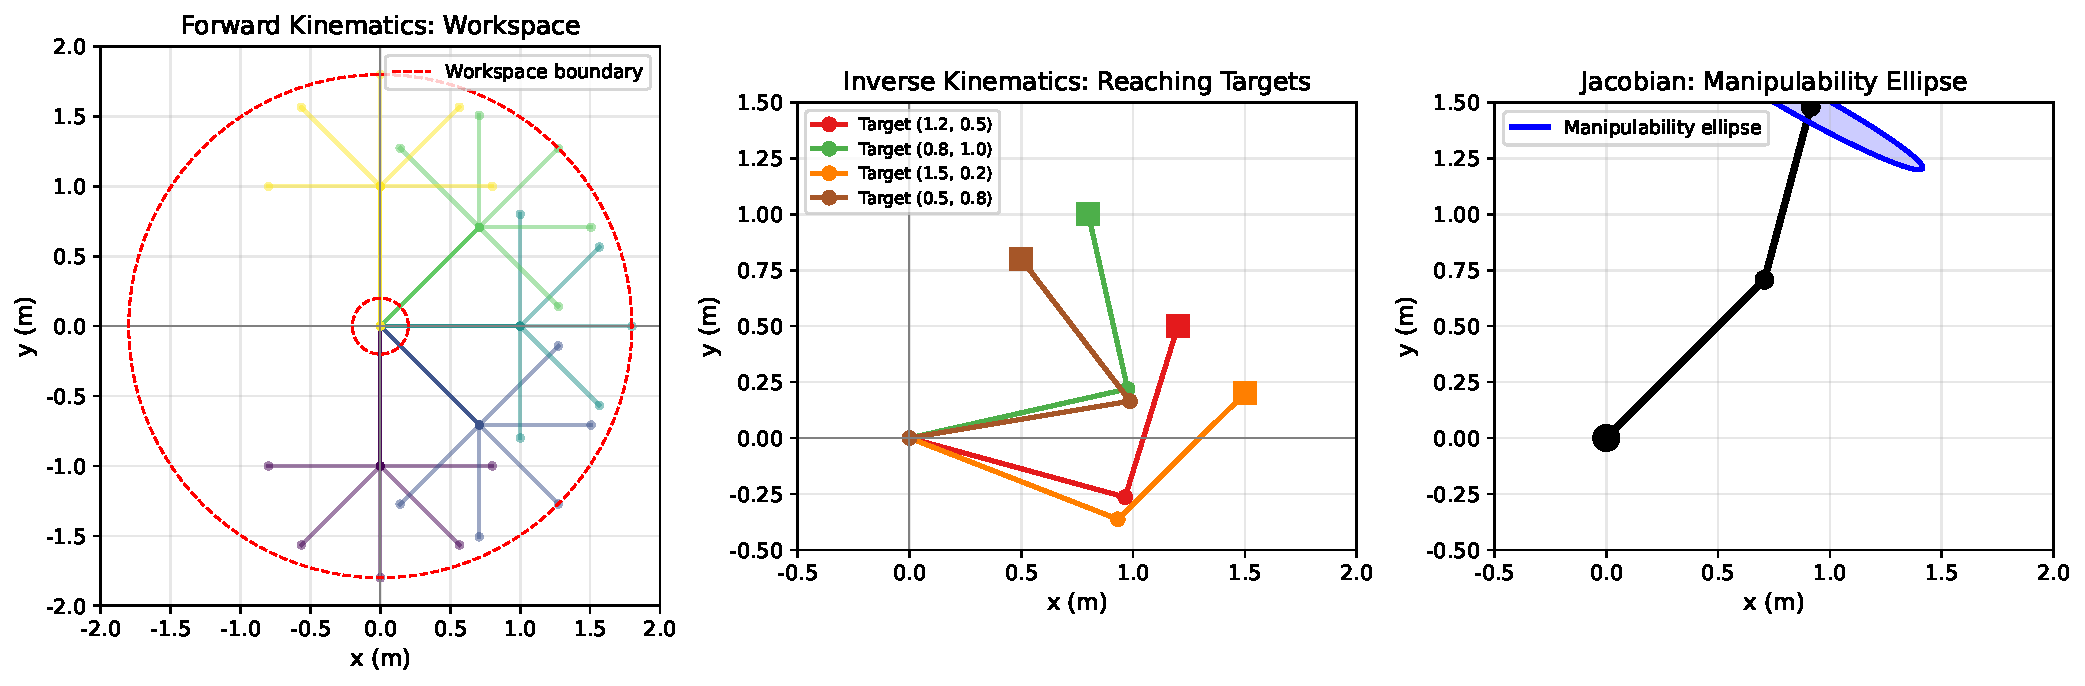
\includegraphics[width=0.95\textwidth]{figs_chap10/arm_kinematics.pdf}
\caption{二连杆机械臂运动学。左图：正运动学——给定关节角度，计算末端位置，扫出工作空间。中图：逆运动学——给定目标位置，求解关节角度。右图：雅可比矩阵决定的"可操作性椭圆"，反映不同方向上的运动能力。}
\label{fig:arm_kinematics}
\end{figure}

\paragraph{正运动学}
给定关节角度$(\theta_1, \theta_2)$，末端位置为：
\begin{align}
    x &= L_1 \cos\theta_1 + L_2 \cos(\theta_1 + \theta_2) \\
    y &= L_1 \sin\theta_1 + L_2 \sin(\theta_1 + \theta_2)
\end{align}

\paragraph{逆运动学}
给定目标位置$(x, y)$，需要求解$(\theta_1, \theta_2)$。这是一个非线性方程组，通常有多个解（对应不同的肘部朝向）。用余弦定理可得：
\[
\cos\theta_2 = \frac{x^2 + y^2 - L_1^2 - L_2^2}{2 L_1 L_2}
\]

\paragraph{雅可比矩阵}
末端速度与关节速度的关系由\textbf{雅可比矩阵}描述：
\[
\begin{pmatrix} \dot{x} \\ \dot{y} \end{pmatrix} = J(\theta) \begin{pmatrix} \dot{\theta}_1 \\ \dot{\theta}_2 \end{pmatrix}
\]

雅可比矩阵的奇异值分解揭示了机械臂在不同方向的"灵活度"——椭圆长轴方向容易运动，短轴方向难以运动。

% ------------------------------------------------------------------------------------
\subsection*{三、传统控制 vs 强化学习}

\begin{figure}[htbp]
\centering
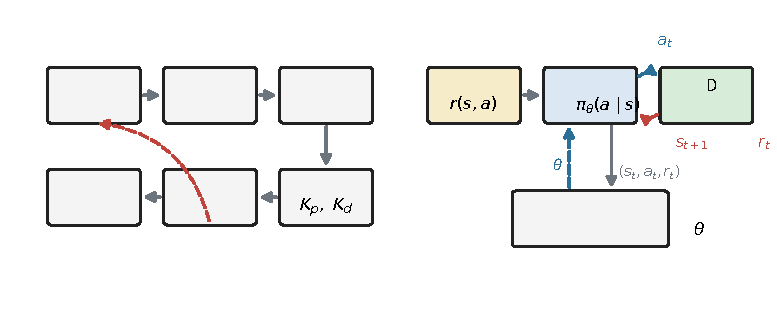
\includegraphics[width=0.95\textwidth]{figs_chap10/rl_control_comparison.pdf}
\caption{控制方法对比。传统控制需要精确建模、控制器设计、稳定性分析；强化学习只需定义奖励函数，让智能体在交互中学习，但需要大量训练样本和计算资源。}
\label{fig:rl_control_comparison}
\end{figure}

\paragraph{传统方法：PD控制}
最简单的控制策略是\textbf{PD控制器}：
\[
\tau = K_p (\theta_{\text{target}} - \theta) - K_d \dot{\theta}
\]

这需要：(1) 知道目标角度（需要逆运动学）；(2) 调节增益$K_p, K_d$；(3) 假设动力学足够简单。

图\ref{fig:pd_control}展示了PD控制器跟踪圆形轨迹的效果——在简单任务上表现良好，但对模型误差和外部扰动敏感。

\begin{figure}[htbp]
\centering
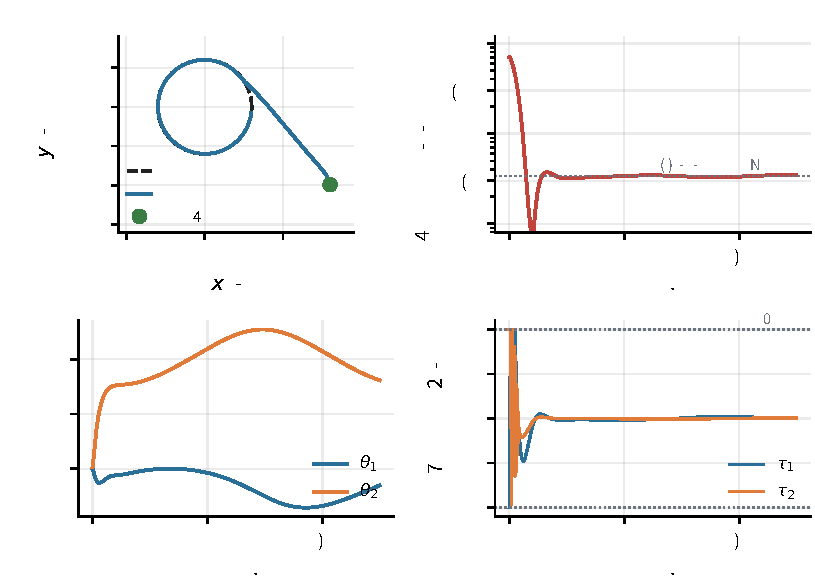
\includegraphics[width=0.95\textwidth]{figs_chap10/pd_control_trajectory.pdf}
\caption{PD控制器跟踪圆形轨迹。左上：末端实际轨迹vs目标轨迹。右上：跟踪误差。左下：关节角度随时间变化。右下：控制力矩。}
\label{fig:pd_control}
\end{figure}

\paragraph{强化学习方法}
RL不需要显式的逆运动学或动力学模型。智能体直接学习从状态到力矩的映射：
\[
\pi_\theta: (\theta_1, \theta_2, \dot{\theta}_1, \dot{\theta}_2, x_{\text{goal}}, y_{\text{goal}}) \mapsto (\tau_1, \tau_2)
\]

奖励设计示例：
\[
r = -\|p_{\text{end}} - p_{\text{goal}}\|^2 - 0.01 \|\tau\|^2
\]
第一项鼓励接近目标，第二项惩罚过大的力矩。

% ------------------------------------------------------------------------------------
\subsection*{四、CartPole：连续控制的入门任务}

在动手实现机械臂RL之前，先用更简单的\textbf{CartPole}任务热身（图\ref{fig:cartpole_demo}）。

\begin{figure}[htbp]
\centering
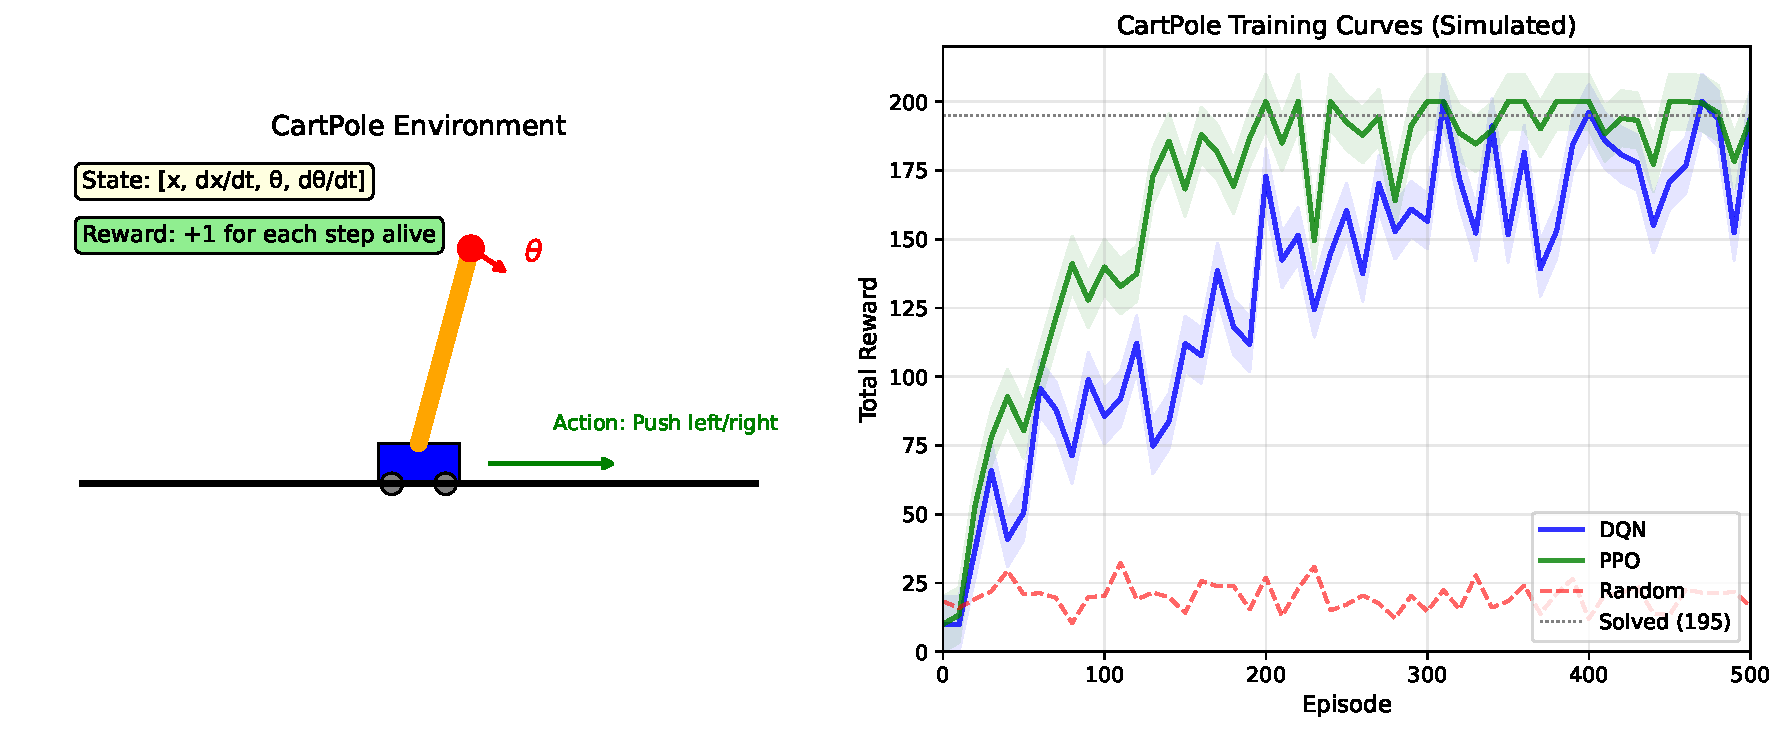
\includegraphics[width=0.95\textwidth]{figs_chap10/cartpole_demo.pdf}
\caption{CartPole任务。左图：环境示意——小车上竖立一根杆，目标是通过左右推动小车让杆保持竖直。状态是4维连续向量，动作是离散的（左/右）。右图：不同算法的学习曲线（模拟）——PPO和DQN都能在几百个episode内学会，随机策略则始终徘徊在低奖励。}
\label{fig:cartpole_demo}
\end{figure}

CartPole的状态是4维向量$[x, \dot{x}, \theta, \dot{\theta}]$，目标是让杆保持竖直（$|\theta| < 12°$）且小车不出界（$|x| < 2.4$）。每坚持一步获得+1奖励，达到200步"solved"。

\paragraph{用Stable Baselines3训练}

\begin{lstlisting}[language=Python]
import gymnasium as gym
from stable_baselines3 import PPO

# 创建环境
env = gym.make("CartPole-v1")

# 创建并训练智能体
model = PPO("MlpPolicy", env, verbose=1)
model.learn(total_timesteps=50000)

# 测试
obs, _ = env.reset()
for _ in range(200):
    action, _ = model.predict(obs, deterministic=True)
    obs, reward, done, truncated, info = env.step(action)
    if done:
        break
\end{lstlisting}

PPO（Proximal Policy Optimization）是目前最常用的策略梯度算法，在ChatGPT的RLHF训练中也使用了它。

% ------------------------------------------------------------------------------------
\subsection*{五、进阶：用RL控制机械臂}

机械臂控制比CartPole复杂得多：
\begin{itemize}
    \item 动作空间是\textbf{连续}的（力矩值），需要用SAC或TD3等算法
    \item 状态维度更高（关节+目标位置）
    \item 奖励设计更关键（稀疏奖励很难学习）
\end{itemize}

推荐使用\texttt{gymnasium-robotics}库中的\texttt{FetchReach}等环境，或者MuJoCo物理引擎中的机械臂任务。

\begin{lstlisting}[language=Python]
import gymnasium as gym
from stable_baselines3 import SAC

# 机械臂到达任务（需要安装gymnasium-robotics）
env = gym.make("FetchReach-v3")

# SAC适合连续动作空间
model = SAC("MultiInputPolicy", env, verbose=1)
model.learn(total_timesteps=100000)
\end{lstlisting}

% ------------------------------------------------------------------------------------
\subsection*{六、实践建议}

\begin{insightbox}[title=连续控制学习路线]
\begin{enumerate}
    \item \textbf{入门}：CartPole + DQN/PPO，理解基本训练流程
    \item \textbf{进阶}：Pendulum/MountainCarContinuous + SAC，体验连续动作空间
    \item \textbf{挑战}：FetchReach/HalfCheetah，接触真实机器人仿真
    \item \textbf{实战}：sim-to-real迁移，将仿真策略部署到真实机器人
\end{enumerate}
\end{insightbox}

完整代码见\texttt{code\_chap10/robotic\_arm\_control.py}。

\begin{remark}
从GridWorld到机械臂，我们看到了强化学习的通用性：只要能定义状态、动作、奖励，同样的算法框架就能应用。但"能应用"不等于"好用"——连续控制的样本效率、奖励设计、sim-to-real差距都是活跃的研究方向。
\end{remark}
  % 第10章：强化学习
% ====================================================================================
\chapter{序列建模：从RNN到Transformer}
% ====================================================================================

\section*{Attention Is All You Need}

\sidenoteplain{2017年Google团队发表“Attention Is All You Need”，提出Transformer，彻底改变了NLP。论文标题模仿Beatles的歌“All You Need Is Love”。这个架构成为GPT、BERT、ChatGPT的基础。}

ChatGPT、GPT-4、Claude——这些震惊世界的AI系统都基于同一个架构：\textbf{Transformer}。为什么它能取代统治自然语言处理（NLP）十年的循环神经网络（RNN）？

本章我们将从两个视角回答这个问题。优化视角问的是：为什么RNN的梯度会消失或爆炸？信息论视角问的是：为什么RNN会“遗忘”长距离信息？两个问题的答案指向同一个根源。然后，我们将从零开始构建Transformer，理解它的每一个组件。

\vspace{0.3cm}
\noindent\textit{为什么一个只有几百万参数的 RNN 记不住 50 个词之前的信息？为什么“注意力”这个看似工程化的技巧，会和第4章的最大熵原理长得一模一样？为什么 Transformer 要给残差连接留一条“高速公路”？}

\begin{quote}
\textbf{本章目标}：把序列建模看成“序列损失 + 隐状态递推约束”的拉格朗日问题。你会发现 RNN 的梯度消失就是乘子 $\lambda_t$（隐状态的影子价格）沿时间指数折损，LSTM 的门控和 Transformer 的残差流都是在保护这个影子价格；而注意力的 softmax 则是第4章最大熵原理的直接产物。读完本章，Q、K、V、缩放、多头、位置编码、残差——都不再是“设计出来的”，而是从约束里自然涌现的。
\end{quote}

\begin{tcolorbox}[colback=green!5, colframe=green!60!black, title=学完这章，你将能够...]
\begin{itemize}
    \item 分析RNN为什么会梯度消失，LSTM如何缓解
    \item 手算Self-Attention的输出（给定Q、K、V矩阵）
    \item 解释为什么Transformer能处理长序列
    \item 用PyTorch实现一个简化版Transformer块
    \item 理解GPT、BERT等大模型的架构差异
\end{itemize}
\end{tcolorbox}

% ====================================================================================
\section{RNN：序列建模的第一次尝试}
% ====================================================================================

在理解Transformer之前，我们需要先理解它的前辈——循环神经网络（Recurrent Neural Network, RNN）。
\storynote{Sepp Hochreiter}{1991年，慕尼黑工大的硕士生 Hochreiter 在 Schmidhuber 指导下写出一篇德文论文，第一次从数学上解释了 RNN 的梯度消失；六年后两人提出 LSTM。这篇论文直到 2000 年代才被英语世界广泛引用——“Attention Is All You Need”其实是在回答他 26 年前提出的问题。}

% ------------------------------------------------------------------------------------
\subsection{序列建模作为约束优化问题}
% ------------------------------------------------------------------------------------

序列数据的特点是每一步都依赖于之前的历史。我们要回答的第一个问题是：这种依赖应该怎样写进优化问题？让我们用熟悉的约束优化框架来理解序列建模——答案是把“依赖历史”写成一条约束。

\begin{keyidea}[序列模型的统一形式]
所有序列模型都可以写成以下约束优化问题：
\begin{equation}
    \begin{aligned}
        \min_{\{h_t\}, \theta} \quad & J = \sum_{t=1}^{T} \ell(h_t, y_t) \\
        \text{s.t.} \quad & h_{t+1} = F(h_t, x_t; \theta) \quad \text{（动力学/机器学习模型约束）}
    \end{aligned}
\end{equation}
其中 $h_t$ 是第 $t$ 步的\textbf{隐状态}（Hidden State），压缩了历史信息；$x_t$ 是第 $t$ 步的\textbf{输入}（如当前单词）；$y_t$ 是第 $t$ 步的\textbf{目标}（如下一个单词）；$\theta$ 是\textbf{模型参数}；$F$ 是\textbf{状态转移函数}。
\end{keyidea}

这和第9章强化学习中看到的结构是一样的！隐状态 $h_t$ 就像MDP中的状态，状态转移函数 $F$ 就像环境的动力学方程。
\think{回顾一下：第3章变分法、第5章力学、第7章轨迹优化、第8章神经网络、第9章强化学习，都有同样的约束结构$x_{t+1} = f(x_t, u_t)$。这不是巧合——它们都是同一个数学框架的不同实例！}

% ------------------------------------------------------------------------------------
\subsection{RNN的动力学方程}
% ------------------------------------------------------------------------------------

RNN选择了最简单的状态转移函数——线性变换加非线性激活：

\begin{keyformula}[title=RNN递推方程]
\begin{equation}
    h_t = \sigma(W_h h_{t-1} + W_x x_t + b)
\end{equation}
其中 $\sigma$ 是激活函数（如tanh），$W_h, W_x, b$ 是可学习参数。
\end{keyformula}
\review{第8章}{激活函数$\sigma$是什么？它是神经网络的“非线性调味料”——没有它，多层网络就退化成单层线性变换。常用的有ReLU、tanh、sigmoid，第8章详细讨论了它们的性质。}

\begin{figure}[htbp]
\centering
\begin{tikzpicture}[>=stealth, scale=0.9]
    % 展开的RNN
    \foreach \i in {0,1,2,3} {
        % 隐状态
        \node[draw, circle, fill=blue!20, minimum size=1cm] (h\i) at (\i*3, 0) {$h_{\i}$};
        % 输入
        \node[draw, rectangle, fill=green!20, minimum width=0.8cm, minimum height=0.6cm] (x\i) at (\i*3, -1.5) {$x_{\i}$};
        % 输出
        \node[draw, rectangle, fill=orange!20, minimum width=0.8cm, minimum height=0.6cm] (y\i) at (\i*3, 1.5) {$y_{\i}$};
        % 连接
        \draw[->, thick] (x\i) -- (h\i);
        \draw[->, thick] (h\i) -- (y\i);
    }
    % 水平连接（共享参数W_h）
    \foreach \i in {0,1,2} {
        \pgfmathtruncatemacro{\j}{\i+1}
        \draw[->, thick, red] (h\i) -- node[above, font=\small] {$W_h$} (h\j);
    }
    % 省略号
    \node at (12.5, 0) {$\cdots$};
    
    % 标注
    \node[below, font=\small, gray] at (4.5, -2.2) {所有时间步共享同一组参数 $W_h, W_x, b$};
\end{tikzpicture}
\caption{RNN的展开图。红色箭头表示同一个矩阵 $W_h$ 被重复使用。}
\end{figure}

\paragraph{关键特点：参数共享}

注意到 $W_h, W_x, b$ 在所有时间步都是\textbf{相同的}。这个设计有深刻的物理原因。第一是\textbf{时间平移对称性}：物理定律不随时间改变，牛顿定律昨天适用，今天也适用；类似地，语言的语法规则在句首和句尾应该是一致的。第二是\textbf{处理任意长度}的需要：参数数量与序列长度无关，所以可以处理任意长的输入。

\begin{tcolorbox}[colback=yellow!10, colframe=orange!80, title=本章的核心观点]
\textbf{序列建模不是什么新东西——它就是第1章的拉格朗日乘子法，只不过约束变成了一条长度为 $T$ 的递推链 $h_{t+1} = F(h_t, x_t; \theta)$，乘子 $\lambda_t$ 变成了“沿时间往回传的梯度”。}

本章的问题就是第1章的问题，只是变量多了 $T$ 组隐状态、约束多了 $T$ 条递推方程，于是乘子也多了 $T$ 个。RNN、LSTM、Transformer 的区别，只在于这 $T$ 条约束的\textbf{拓扑}——一条长链，还是一张短而宽的图。

\begin{center}
\renewcommand{\arraystretch}{1.3}
\small
\begin{tabularx}{\linewidth}{lXX}
\toprule
 & \textbf{第1章（有限维）} & \textbf{本章（序列模型）} \\
\midrule
变量 & $x \in \R^n$ & 隐状态 $h_1, \ldots, h_T$ 与参数 $\theta$ \\
目标 & $f(x)$ & $J = \sum_t \ell(h_t, y_t)$ \\
约束 & $g(x) = 0$ & $F(h_t, x_t; \theta) - h_{t+1} = 0$（$T$ 条） \\
乘子 & $\lambda$ & $\lambda_t = \partial J/\partial h_t$（伴随变量） \\
一阶条件 & $\nabla f + \lambda^\top \nabla g = 0$ & 伴随方程 $\lambda_t = J_t^\top \lambda_{t+1} + \partial \ell/\partial h_t$ \\
影子价格 & $\partial f^*/\partial c$ & 扰动 $h_t$ 一单位，总损失变化多少 \\
病态 & 约束雅可比奇异 & $\prod_t J_t$ 指数消失 / 爆炸 \\
\bottomrule
\end{tabularx}
\end{center}
\end{tcolorbox}

但这个设计也带来了严重的问题——让我们用拉格朗日乘子法来分析。
\review{第7章}{把 $h_t$ 看成状态、$x_t$ 看成外部输入，$h_{t+1} = F(h_t, x_t; \theta)$ 就是第7章轨迹优化里的离散动力学约束。那里对每个时刻引入一个乘子 $\lambda_t$，这里也一样。}

% ------------------------------------------------------------------------------------
% ------------------------------------------------------------------------------------
\subsection{梯度问题：伴随方程的视角}
% ------------------------------------------------------------------------------------

为了训练RNN，我们需要计算损失函数对参数的梯度。让我们用伴随方法（Adjoint Method）来分析。

构造拉格朗日函数：
\begin{equation}
    \mathcal{L} = \sum_{t=1}^{T} \ell(h_t, y_t) + \sum_{t=0}^{T-1} \lambda_{t+1}^\top \left( F(h_t, x_t; \theta) - h_{t+1} \right)
\end{equation}

其中 $\lambda_t$ 是拉格朗日乘子。根据KKT条件，对 $h_t$ 求偏导为零，得到\textbf{伴随方程}（也就是反向传播的数学本质）：

\begin{equation}
    \lambda_t = \left( \frac{\partial F}{\partial h_t} \right)^\top \lambda_{t+1} + \frac{\partial \ell}{\partial h_t}
\end{equation}

这里的 $\lambda_t$ 正是梯度 $\frac{\partial J}{\partial h_t}$。
\clarify{按全书的说法，$\lambda_t$ 是“约束 $h_{t+1} = F(h_t, x_t)$ 的影子价格”：把第 $t$ 步的隐状态推开 $\delta$，总损失变化 $\lambda_t^\top \delta$。第8章里它叫“误差信号”，第7章里叫“协态”，是同一个东西。（约束写成 $F - h_{t+1}$ 而不是 $h_{t+1} - F$，是为了让 $\lambda_t$ 恰好等于 $+\partial J/\partial h_t$，与第7章连续部分一致。）}

\paragraph{各个量的形状}

让我们明确每个量的维度。假设隐状态 $h_t \in \mathbb{R}^n$（$n$ 是隐藏层大小），则：

\begin{table}[htbp]
\centering
\renewcommand{\arraystretch}{1.3}
\begin{tabular}{lll}
\toprule
符号 & 形状 & 含义 \\
\midrule
$h_t$ & $\mathbb{R}^n$ & 时刻 $t$ 的隐状态向量 \\
$W_h$ & $\mathbb{R}^{n \times n}$ & 隐状态到隐状态的权重矩阵 \\
$\lambda_t$ & $\mathbb{R}^n$ & 对 $h_t$ 的梯度（拉格朗日乘子） \\
$\frac{\partial F}{\partial h_t}$ & $\mathbb{R}^{n \times n}$ & 雅可比矩阵（Jacobian） \\
\bottomrule
\end{tabular}
\end{table}

\paragraph{雅可比矩阵的结构}

RNN的状态转移是：
\begin{equation}
    h_{t+1} = F(h_t, x_t) = \sigma(W_h h_t + W_x x_t + b)
\end{equation}

其中 $\sigma$ 是逐元素的激活函数。我们来计算雅可比矩阵 $\frac{\partial h_{t+1}}{\partial h_t}$。

设 $z_t = W_h h_t + W_x x_t + b$（激活前的值），则 $h_{t+1} = \sigma(z_t)$。用链式法则：

\begin{equation}
    \frac{\partial h_{t+1}}{\partial h_t} = \frac{\partial \sigma(z_t)}{\partial z_t} \cdot \frac{\partial z_t}{\partial h_t}
\end{equation}

第二个因子最简单：$\frac{\partial z_t}{\partial h_t} = W_h$，形状是 $n \times n$。第一个因子 $\frac{\partial \sigma(z_t)}{\partial z_t} = \text{diag}(\sigma'(z_t))$ 是一个 $n \times n$ 的\textbf{对角矩阵}，这是因为 $\sigma$ 是逐元素操作：$[\sigma(z)]_i = \sigma(z_i)$，所以
\begin{equation}
    \frac{\partial [\sigma(z)]_i}{\partial z_j} = \begin{cases}
        \sigma'(z_i) & \text{if } i = j \\
        0 & \text{if } i \neq j
    \end{cases}
\end{equation}

因此，雅可比矩阵是：

\begin{keyformula}[title=RNN的雅可比矩阵]
\begin{equation}
    J_t := \frac{\partial h_{t+1}}{\partial h_t} = \text{diag}(\sigma'(z_t)) \cdot W_h \in \mathbb{R}^{n \times n}
\end{equation}
其中 $\text{diag}(\sigma'(z_t))$ 是对角线上放置 $\sigma'(z_{t,1}), \sigma'(z_{t,2}), \ldots, \sigma'(z_{t,n})$ 的对角矩阵。
\end{keyformula}

\begin{figure}[htbp]
\centering
\begin{tikzpicture}[scale=0.62]
    % 对角矩阵
    \node at (2, 4.5) {$\text{diag}(\sigma'(z_t))$};
    \draw[thick] (0, 0) rectangle (4, 4);
    \fill[blue!30] (0, 3) rectangle (1, 4);
    \fill[blue!30] (1, 2) rectangle (2, 3);
    \fill[blue!30] (2, 1) rectangle (3, 2);
    \fill[blue!30] (3, 0) rectangle (4, 1);
    \node[font=\scriptsize] at (0.5, 3.5) {$\sigma'_1$};
    \node[font=\scriptsize] at (1.5, 2.5) {$\sigma'_2$};
    \node[font=\scriptsize] at (2.5, 1.5) {$\sigma'_3$};
    \node[font=\scriptsize] at (3.5, 0.5) {$\sigma'_n$};
    \node at (2, -0.5) {$n \times n$};
    
    % 乘号
    \node at (5, 2) {$\times$};
    
    % W_h矩阵
    \node at (8, 4.5) {$W_h$};
    \draw[thick] (6, 0) rectangle (10, 4);
    \fill[green!20] (6, 0) rectangle (10, 4);
    \node at (8, 2) {稠密};
    \node at (8, -0.5) {$n \times n$};
    
    % 等号
    \node at (11, 2) {$=$};
    
    % 结果
    \node at (14, 4.5) {$J_t$};
    \draw[thick] (12, 0) rectangle (16, 4);
    \fill[orange!20] (12, 0) rectangle (16, 4);
    \node at (14, 2) {雅可比};
    \node at (14, -0.5) {$n \times n$};
\end{tikzpicture}
\caption{雅可比矩阵的结构：对角矩阵（激活函数导数）乘以权重矩阵}
\end{figure}

\paragraph{梯度的矩阵连乘}

从时刻 $T$ 反向传播到时刻 $0$，需要连乘所有时刻的雅可比矩阵：

\begin{equation}
    \frac{\partial J}{\partial h_0} = \frac{\partial J}{\partial h_T} \cdot \prod_{t=0}^{T-1} J_t^\top = \frac{\partial J}{\partial h_T} \cdot J_{T-1}^\top \cdot J_{T-2}^\top \cdots J_1^\top \cdot J_0^\top
\end{equation}

展开写：
\begin{equation}
    \frac{\partial J}{\partial h_0} = \frac{\partial J}{\partial h_T} \cdot \prod_{t=0}^{T-1} W_h^\top \cdot \text{diag}(\sigma'(z_t))
\end{equation}

\begin{figure}[htbp]
\centering
\begin{tikzpicture}[>=stealth, scale=0.8]
    % 梯度向量
    \node[draw, rectangle, fill=red!20, minimum width=1cm, minimum height=1.5cm] (grad) at (0, 0) {$\frac{\partial J}{\partial h_T}$};
    \node[below, font=\scriptsize] at (0, -1) {$1 \times n$};
    
    % 连乘的矩阵
    \foreach \i/\label in {1/T-1, 2/T-2, 3/\cdots, 4/0} {
        \pgfmathsetmacro{\x}{1.5 + \i*2}
        \node[draw, rectangle, fill=blue!20, minimum width=1.5cm, minimum height=1.5cm] (J\i) at (\x, 0) {$J_{\label}^\top$};
        \node[below, font=\scriptsize] at (\x, -1) {$n \times n$};
    }
    
    % 乘号
    \node at (1, 0) {$\times$};
    \node at (4.5, 0) {$\times$};
    \node at (6.5, 0) {$\times$};
    \node at (8.5, 0) {$\times$};
    
    % 结果
    \node at (11, 0) {$=$};
    \node[draw, rectangle, fill=green!20, minimum width=1cm, minimum height=1.5cm] (result) at (13, 0) {$\frac{\partial J}{\partial h_0}$};
    \node[below, font=\scriptsize] at (13, -1) {$1 \times n$};
    
    % 标注
    \draw[decorate, decoration={brace, amplitude=8pt, mirror}] (2.5, -2) -- (9.5, -2);
    \node[below] at (6, -2.5) {连乘 $T$ 个 $n \times n$ 矩阵};
\end{tikzpicture}
\caption{梯度反向传播需要连乘 $T$ 个雅可比矩阵}
\end{figure}

\paragraph{问题的根源}

虽然每个时刻的 $\text{diag}(\sigma'(z_t))$ 不同，但 $W_h$ 是\textbf{同一个矩阵}！

考虑简化情况，假设 $\sigma' \approx 1$（线性激活），则：
\begin{equation}
    \frac{\partial J}{\partial h_0} \approx \frac{\partial J}{\partial h_T} \cdot (W_h^\top)^T
\end{equation}

这就是同一个矩阵的 $T$ 次幂！

\paragraph{特征值分析}

设 $W_h$ 的特征分解为 $W_h = P \Lambda P^{-1}$，其中 $\Lambda = \text{diag}(\mu_1, \ldots, \mu_n)$ 是特征值对角矩阵（这里用 $\mu$ 记特征值，把 $\lambda$ 留给乘子）。则：

\begin{equation}
    W_h^T = P \Lambda^T P^{-1} = P \cdot \text{diag}(\mu_1^T, \ldots, \mu_n^T) \cdot P^{-1}
\end{equation}

设最大特征值的模为 $\rho = \max_i |\mu_i|$。若 $\rho < 1$，则 $|\mu_i|^T \to 0$，梯度\textbf{指数衰减}；若 $\rho > 1$，则 $|\mu_i|^T \to \infty$，梯度\textbf{指数爆炸}；只有 $\rho = 1$ 时理论上稳定，但实际中难以精确控制。
\think{把 $W_h$ 换成正交矩阵（所有特征值模为 1），连乘还会爆炸或消失吗？非线性 $\sigma'$ 又会把这个结论破坏到什么程度？（提示：这就是“酉 RNN”的出发点。）}

\begin{example}[梯度消失的数值演示]
假设隐状态维度 $n = 256$，$W_h$ 的最大特征值 $\rho = 0.9$，序列长度 $T = 100$。

沿最大特征向量方向的梯度衰减：
\begin{equation}
    0.9^{100} \approx 2.66 \times 10^{-5}
\end{equation}

这意味着从位置 100 传回位置 0 的梯度只剩下原来的 $0.003\%$！模型几乎无法学习长距离依赖。

反过来，若 $\rho = 1.1$：
\begin{equation}
    1.1^{100} \approx 1.38 \times 10^{4}
\end{equation}

梯度会爆炸到上万倍，训练变得极不稳定，loss可能变成NaN。
\end{example}

\sidenoteplain{对于tanh激活函数，$|\sigma'(z)| \leq 1$，这进一步加剧了梯度消失。因为每一步都要乘以一个 $\leq 1$ 的因子。}


% ------------------------------------------------------------------------------------
\subsection{信息论视角：数据处理不等式}
% ------------------------------------------------------------------------------------

除了梯度问题，RNN还有一个更根本的信息论限制。即使我们想办法把梯度传回去，前向传播时信息是不是已经丢了？

\begin{keyidea}[RNN的信息瓶颈]
RNN的状态更新具有马尔可夫性：
\begin{equation}
    X_{<t} \to h_{t-1} \to h_t \to X_{t+1}
\end{equation}
所有历史信息 $X_{<t}$ 必须通过一个固定大小的向量 $h_t$ 传递给未来。
\end{keyidea}

根据\textbf{数据处理不等式}（Data Processing Inequality）：

\begin{equation}
    I(X_{<t}; h_{t+k}) \leq I(X_{<t}; h_{t+k-1}) \leq \cdots \leq I(X_{<t}; h_t)
\end{equation}
（固定“过去” $X_{<t}$，让隐状态往后走：每走一步，隐状态里关于过去的信息只会减少。）

\begin{figure}[htbp]
\centering
\begin{tikzpicture}[>=stealth, scale=0.9]
    % 信息流
    \node[draw, rectangle, fill=green!20, minimum width=1.5cm] (x0) at (0, 0) {$X_{<t}$};
    \node[draw, circle, fill=blue!20, minimum size=1cm] (h1) at (3, 0) {$h_t$};
    \node[draw, circle, fill=blue!20, minimum size=1cm] (h2) at (6, 0) {$h_{t+1}$};
    \node[draw, circle, fill=blue!20, minimum size=1cm] (h3) at (9, 0) {$h_{t+2}$};
    \node[draw, rectangle, fill=orange!20, minimum width=1.5cm] (xf) at (12, 0) {$X_{t+k}$};
    
    % 箭头
    \draw[->, thick] (x0) -- node[above, font=\small] {压缩} (h1);
    \draw[->, thick] (h1) -- (h2);
    \draw[->, thick] (h2) -- (h3);
    \draw[->, thick, dashed] (h3) -- (xf);
    
    % 信息量标注
    \draw[<->, red] (0, -1) -- (3, -1);
    \node[below, red, font=\small] at (1.5, -1) {信息损失};
    
    \draw[<->, red] (3, -1) -- (6, -1);
    \node[below, red, font=\small] at (4.5, -1) {继续损失};
    
    % 瓶颈标注
    \node[below, font=\small, gray] at (6, -2) {固定大小的“瓶颈”不断压缩信息};
\end{tikzpicture}
\caption{RNN的信息瓶颈：历史信息被强制压缩进固定大小的隐状态}
\end{figure}

这意味着信息只能\textbf{减少}，不能增加，而且距离越远，能保留的信息越少。这是\textbf{有损压缩}，信息随距离单调衰减（有限容量的隐状态下通常是指数式的）。

\begin{remark}
长距离依赖的丢失不仅是梯度问题，更是\textbf{信息论的必然}。即使梯度完美传播，信息也已经在前向传播中丢失了。
\end{remark}

% ====================================================================================
\section{LSTM：门控的缓解尝试}
% ====================================================================================

\sidenoteplain{\textbf{LSTM的历史}：LSTM由德国学者Sepp Hochreiter和Jürgen Schmidhuber于1997年提出。Hochreiter在博士论文中分析了RNN梯度消失问题，LSTM的门控设计正是为了解决这个问题。2010年代LSTM在语音识别（Google Voice）和机器翻译中大放异彩，直到2017年被Transformer取代。}

上一节的诊断是：同一个雅可比连乘 $T$ 次。既然如此，能不能让某条通路上的雅可比接近单位阵？长短期记忆网络（LSTM）试图通过\textbf{门控机制}来缓解梯度问题。

% ------------------------------------------------------------------------------------
\subsection{LSTM的核心设计}
% ------------------------------------------------------------------------------------

LSTM引入了一个新的状态——\textbf{细胞状态}（Cell State）$c_t$，以及三个“门”来控制信息流：

\begin{keyformula}[title=LSTM方程]
\begin{align}
    f_t &= \sigma(W_f [h_{t-1}, x_t] + b_f) \quad \text{（遗忘门）} \\
    i_t &= \sigma(W_i [h_{t-1}, x_t] + b_i) \quad \text{（输入门）} \\
    \tilde{c}_t &= \tanh(W_c [h_{t-1}, x_t] + b_c) \quad \text{（候选记忆）} \\
    c_t &= f_t \odot c_{t-1} + i_t \odot \tilde{c}_t \quad \text{（记忆更新）} \\
    o_t &= \sigma(W_o [h_{t-1}, x_t] + b_o) \quad \text{（输出门）} \\
    h_t &= o_t \odot \tanh(c_t) \quad \text{（隐状态）}
\end{align}
其中 $\odot$ 表示逐元素乘法，$\sigma$ 是sigmoid函数（输出在0到1之间）。
\end{keyformula}
\storynote{Yoshua Bengio}{1964--，2018年图灵奖得主，蒙特利尔大学教授，被称为``深度学习三巨头''之一。他对序列模型贡献巨大：他和学生提出了神经机器翻译、注意力机制的早期版本，以及GAN的改进。他创立的MILA是全球最大的AI研究机构之一。}

\begin{figure}[htbp]
\centering
\begin{tikzpicture}[>=stealth, scale=0.7, font=\small]

\tikzstyle{layer} = [draw, thick, fill=yellow!20, minimum width=1cm, minimum height=0.6cm]
\tikzstyle{op} = [draw, thick, circle, fill=green!10, inner sep=0pt, minimum size=0.6cm]
\tikzstyle{labeltext} = [font=\scriptsize, color=gray!80!black]

\draw[thick, rounded corners=8pt, fill=gray!5] (0, 0) rectangle (13, 6);

% --- 遗忘门
\node[layer] (ft) at (2.5, 2) {$f_t$};
\node[op] (mul_f) at (2.5, 5) {$\times$};
\node[labeltext, below=0.2cm] at (ft.south) {遗忘门};

% --- 输入门
\node[layer] (it) at (5.5, 2) {$i_t$};
\node[layer, fill=purple!10] (ct_tilde) at (7.5, 2) {$\tilde{c}_t$};
\node[op] (mul_i) at (6.5, 3.5) {$\times$};
\node[op] (add_c) at (6.5, 5) {$+$};

% --- 输出门
\node[layer] (ot) at (10.5, 2) {$o_t$};
\node[op, fill=white] (tanh_out) at (10.5, 3.8) {\footnotesize tanh};
\node[op] (mul_h) at (10.5, 2.8) {$\times$};

% --- Cell State 顶部高速通道
\coordinate (c_in) at (-1.2, 5);
\coordinate (c_out) at (14.2, 5);

\draw[->, very thick, blue!70!black] (c_in) -- (mul_f);
\draw[->, very thick, blue!70!black] (mul_f) -- (add_c);
\draw[->, very thick, blue!70!black] (add_c) -- (c_out);

\node[left] at (c_in) {$c_{t-1}$};
\node[right] at (c_out) {$c_t$};

% --- Input bus
\coordinate (input_entry) at (6.5, -1.2);

\node[below] at (input_entry) {输入 $x_t, h_{t-1}$};

\draw[thick] (input_entry) -- (6.5, 0.8);   

\draw[->, thick] (6.5, 0.8) -| (ft.south);
\draw[->, thick] (6.5, 0.8) -| (it.south);
\draw[->, thick] (6.5, 0.8) -| (ct_tilde.south);
\draw[->, thick] (6.5, 0.8) -| (ot.south);

% 遗忘门连通
\draw[->, thick] (ft.north) -- (mul_f.south);

% 输入门和候选状态融合
\draw[->, thick] (it.north) |- (mul_i.west);
\draw[->, thick] (ct_tilde.north) |- (mul_i.east);
\draw[->, thick] (mul_i.north) -- (add_c.south);

% 输出路径
\draw[fill=black] (8.5, 5) circle (0.08);
\draw[->, thick] (8.5, 5) |- (tanh_out.west);

\draw[->, thick] (tanh_out.south) -- (mul_h.north);
\draw[->, thick] (ot.north) -- (mul_h.south);

\draw[->, very thick] (mul_h.east) -- (14.2, 2.8) node[right] {$h_t$};

\end{tikzpicture}
\caption{LSTM 内部详细数据流向图}
\end{figure}


\paragraph{门控如何帮助梯度传播？}

关键在于细胞状态的更新方程：
\begin{equation}
    c_t = f_t \odot c_{t-1} + i_t \odot \tilde{c}_t
\end{equation}

对应的梯度（伴随方程）：
\begin{equation}
    \frac{\partial c_t}{\partial c_{t-1}} = \text{diag}(f_t)
\end{equation}

当遗忘门 $f_t \approx 1$ 时，梯度可以近乎无损地传播！这就像在动力系统中加入了一条“梯度高速公路”。
\preview{“梯度高速公路”在本章后面的残差流、第14章 PINN 的深层网络里都会再出现：让主干通路的雅可比接近单位阵，影子价格就不会折损。}

\paragraph{LSTM的局限}

尽管LSTM缓解了梯度消失，它仍然有根本性的限制。它仍是串行计算，$h_t$ 依赖 $h_{t-1}$，无法并行；路径长度仍是 $O(T)$，信息必须经过 $T$ 步才能从开头传到结尾；信息瓶颈也依然存在，所有历史仍被压缩进固定大小的状态。

\begin{remark}
LSTM把“结构性的梯度消失问题”转化为了“可学习的优化问题”——让模型自己决定遗忘什么、记住什么。但这只是缓解，不是根治。在 $T \to \infty$ 的极限下，重复应用同一个算子必然导致信息退化。
\end{remark}

% ====================================================================================
\section{为什么参数必须共享？}
% ====================================================================================

在继续之前，让我们思考一个深刻的问题：为什么RNN/LSTM要坚持参数共享？如果每个时间步用不同的参数，不就没有连乘问题了吗？

\think{ResNet每层参数不同，可以做到上千层。为什么RNN做不到？}

% ------------------------------------------------------------------------------------
\subsection{物理约束：时间平移对称性}
% ------------------------------------------------------------------------------------

参数共享源于两个基本假设。

\paragraph{1. 时间平移对称性}

物理定律不随时间改变。牛顿定律 $F = ma$ 昨天成立，今天也成立，明天还成立。类似地，语言的规则也应该是时间无关的：“主语 + 谓语 + 宾语”的结构在句首和句尾都适用，“I love you”和“You love me”遵循相同的语法规则。

\textbf{数学推论}：状态转移函数 $F$ 的参数 $\theta$ 不能依赖于时间 $t$。

\paragraph{2. 因果性}

现在的状态由过去决定，未来不能影响过去。这要求状态必须\textbf{迭代演化}：
\begin{equation}
    h_t = F(h_{t-1}, x_t; \theta)
\end{equation}

\paragraph{代价}

这两个“物理正确”的假设，强行锁定了优化的拓扑结构：参数共享意味着同一矩阵连乘，于是梯度呈指数行为；因果性意味着串行计算，于是无法并行。

\begin{center}
\textit{RNN的悲剧在于：它为了遵守“时间对称性”和“因果性”，牺牲了“优化的稳定性”。}
\end{center}

% ------------------------------------------------------------------------------------
\subsection{对比：为什么ResNet能做深？}
% ------------------------------------------------------------------------------------

\storynote{何恺明}{ResNet（Deep Residual Learning for Image Recognition, 2016）由微软亚洲研究院的何恺明等人提出，获得CVPR 2016最佳论文奖。这篇论文引用量超过20万次，是深度学习领域被引用最多的论文之一。残差连接的思想看似简单，却彻底改变了深度网络的设计范式。}

ResNet和LSTM看起来都有残差结构，为什么表现天差地别？

\begin{table}[htbp]
\centering
\renewcommand{\arraystretch}{1.4}
\begin{tabularx}{\textwidth}{p{2.4cm}|X|X}
\toprule
& \textbf{ResNet（空间深度）} & \textbf{RNN/LSTM（时间深度）} \\
\midrule
\textbf{递推方程} & $x_{\ell+1} = x_\ell + F(x_\ell; \theta_\ell)$ & $h_{t+1} = F(h_t; \theta)$（LSTM 的细胞态才有 $c_{t+1} = c_t + \cdots$） \\
\midrule
\textbf{参数} & 每层不同 $\theta_\ell$ & 所有时间步共享 $\theta$ \\
\midrule
\textbf{动力学性质} & 非自治系统，每层可以纠正上层偏差 & 迭代函数系统，微小偏差被指数放大 \\
\midrule
\textbf{梯度路径} & 穿过 $L$ 个\textbf{不同}的算子 & 同一个算子的 $T$ 次幂 \\
\midrule
\textbf{可行深度} & 1000+层 & 几百步就困难 \\
\bottomrule
\end{tabularx}
\caption{ResNet vs RNN：参数共享的代价}
\end{table}

\textbf{核心结论}：LSTM的门控只能缓解，无法根治。因为在长序列极限下，重复应用同一个算子必然导致动力学行为的退化。


% ====================================================================================
\section{Transformer：打破串行的束缚}
% ====================================================================================

\sidenoteplain{\textbf{Transformer的诞生}：2017年Google团队（Vaswani等8人）发表``Attention Is All You Need''。Ashish Vaswani是第一作者，但这是典型的团队合作成果。这篇论文的引用量已超20万次，是AI史上最具影响力的论文之一。有趣的是，论文的8位作者后来大多离开Google创业。}

上一节的结论是：只要坚持参数共享和串行递推，连乘就无法避免。那么，哪一条假设可以放弃？Transformer的核心洞察是：\textbf{放弃因果性的串行约束，让所有位置直接相连}。

% ------------------------------------------------------------------------------------
\subsection{从时间深度到空间深度}
% ------------------------------------------------------------------------------------

\begin{figure}[htbp]
\centering
\begin{tikzpicture}[>=stealth, scale=0.9, auto]
    % 通用样式
    \tikzstyle{node_rnn} = [circle, draw=blue!80, fill=blue!10, thick, minimum size=0.9cm]
    \tikzstyle{node_trans} = [circle, draw=green!60!black, fill=green!10, thick, minimum size=0.9cm]
    \tikzstyle{arrow_rnn} = [->, thick, blue!80]
    \tikzstyle{line_att} = [-, thick, green!40!black, opacity=0.3]

    % ================= RNN部分 =================
    \begin{scope}[xshift=-5.5cm]
        \node[font=\bfseries] at (2.5, 3) {RNN: 时间串行 (Sequential)};
        
        % 节点
        \foreach \i in {0,1,2,3,4} {
            \node[node_rnn] (r\i) at (\i*1.3, 0) {$h_\i$};
        }
        
        % 串行连接
        \foreach \i [count=\j] in {0,1,2,3} {
            \draw[arrow_rnn] (r\i) -- (r\j);
        }
        
        % 强调长路径
        \draw[<->, red, dashed, thick] (0, -0.8) -- (5.2, -0.8);
        \node[red, below, font=\small] at (2.6, -0.8) {梯度路径长 $O(T)$};
        
        % 隐喻：像接力赛
        \node[gray, font=\footnotesize] at (2.6, -1.5) {必须等待上一步完成};
    \end{scope}

    % ================= Transformer部分 =================
    \begin{scope}[xshift=2cm]
        \node[font=\bfseries] at (2.5, 3) {Transformer: 全局并行 (Parallel)};
        
        % 节点
        \foreach \i in {0,1,2,3,4} {
            \node[node_trans] (t\i) at (\i*1.3, 0) {$x_\i$};
        }
        
        % 全连接 (使用不同曲率的弧线，避免重叠)
        \foreach \i in {0,1,2,3,4} {
            \foreach \j in {0,1,2,3,4} {
                \ifnum\i<\j
                    % 计算弯曲度，距离越远弯曲越大
                    \pgfmathsetmacro{\bendangle}{30 + (\j-\i)*10}
                    \draw[line_att, bend left=\bendangle] (t\i) to (t\j);
                \fi
            }
        }
        
        % 高亮一条长距离连接，展示优势
        \draw[<->, red, very thick, bend left=60] (t0) to node[above, font=\small] {直接相连 $O(1)$} (t4);
        
        % 隐喻：像会议室讨论
        \node[gray, font=\footnotesize] at (2.6, -1.5) {所有人同时对话};
    \end{scope}

    % 分割线
    \draw[dashed, gray!50] (-1, 3.5) -- (-1, -2);

\end{tikzpicture}
\caption{序列建模的两种范式对比：RNN必须按时间步“接力”传递信息，而Transformer允许任意两个位置通过注意力机制“直接对话”。}
\end{figure}

Transformer的关键变化有三点。第一，\textbf{每层参数不同}：第 $\ell$ 层有自己的参数 $\theta^{(\ell)}$，避免连乘同一矩阵。第二，\textbf{注意力机制}：任意两个位置可以直接交互，路径长度 $O(1)$。第三，\textbf{可并行计算}：所有位置可以同时处理。

\paragraph{代价}

Transformer用 $O(T^2)$ 的计算复杂度换取了优化的稳定性。这在现代GPU上是可接受的。
\preview{$O(T^2)$ 到底费多少显存、多少算力？附录C会给出可以直接套用的估算公式（KV Cache、FLOPs $\approx 6ND$）。}

% ------------------------------------------------------------------------------------
% ------------------------------------------------------------------------------------
\subsection{优化视角：残差流与“高速公路”}
% ------------------------------------------------------------------------------------

从数学结构上看，Transformer 的核心在于其\textbf{残差连接（Residual Connection）}。现代大模型（如 GPT-3, LLaMA）通常采用 \textbf{Pre-Norm} 架构，其单层更新为：

\begin{align}
    H' &= H^{(\ell)} + \text{Attn}(\text{LayerNorm}(H^{(\ell)})) \\
    H^{(\ell+1)} &= H' + \text{MLP}(\text{LayerNorm}(H'))
\end{align}

即先对输入做 LayerNorm，然后过 Attention/MLP，最后与原输入相加。这保证了主干通路 $H$ 上没有任何非线性操作，梯度可以无阻碍地流动。

\sidenoteplain{\textbf{Pre-Norm vs. Post-Norm}:
最早的 Transformer（2017）将 Norm 放在残差相加之后（Post-Norm）：$H \leftarrow \text{Norm}(H + \text{Attn}(H))$。现代大模型为了训练稳定性，普遍改用 Pre-Norm：先 Norm 再过子层。Pre-Norm 让残差主干成为一条“高速公路”，是训练超深 Transformer 的关键。}

这意味着，信息和梯度可以沿着 $H$ 通路无损地向前或向后传播，不被非线性层阻断。这也是 Transformer 能够堆叠到近百层（如 GPT-3 的 96 层）而不发生梯度消失的根本数学原因。

\paragraph{现代变体 (SOTA Tricks)}
在实际工程中，为了进一步提升稳定性与效率，还会采用一些改进：RMSNorm 是简化的 LayerNorm，去除了均值中心化，被 DeepSeek/LLaMA 采用；SwiGLU 是更高效的激活函数，替代了传统的 ReLU；RoPE（旋转位置编码）则通过复数旋转引入位置信息。

\begin{table}[htbp]
\centering
\renewcommand{\arraystretch}{1.4}
\begin{tabularx}{\textwidth}{p{2.4cm}|X|X}
\toprule
& \textbf{RNN/LSTM} & \textbf{Transformer} \\
\midrule
\textbf{约束拓扑} & 时间维度的长链（$T$步） & 深度维度的短图（$L$层） \\
\midrule
\textbf{伴随方程} & $\prod_{t=0}^{T} J_t$（连乘） & $\approx I + \epsilon$（残差微扰） \\
\midrule
\textbf{优化难度} & 极难（梯度消失/爆炸） & 容易（平坦的损失曲面） \\
\midrule
\textbf{资源交换} & 省显存，费优化 & 费显存（$O(T^2)$），易优化 \\
\bottomrule
\end{tabularx}
\caption{RNN与Transformer的优化特性对比}
\end{table}

% ------------------------------------------------------------------------------------
% ------------------------------------------------------------------------------------
\subsection{信息论视角：Transformer 为何不丢信息}
% ------------------------------------------------------------------------------------

除了优化视角，我们还可以从\textbf{信息论}角度理解为什么Transformer优于RNN。

\paragraph{RNN的信息瓶颈}

回顾RNN的结构：所有历史信息必须通过一个固定大小的隐状态 $h_t$ 传递。

\begin{equation}
    X_1, X_2, \ldots, X_{t-1} \xrightarrow{\text{压缩}} h_{t-1} \xrightarrow{\text{传递}} h_t \xrightarrow{\text{预测}} X_{t+1}
\end{equation}

根据\textbf{数据处理不等式}（Data Processing Inequality, DPI）：

\begin{keytheorem}[title=数据处理不等式]
对于马尔可夫链 $X \to Y \to Z$，有：
\begin{equation}
    I(X; Z) \leq I(X; Y)
\end{equation}
即信息只能减少，不能增加。数据每经过一次处理，信息只会损失或保持，不可能凭空产生。
\end{keytheorem}

应用到RNN：
\begin{equation}
    I(X_{<t}; h_{T}) \leq I(X_{<t}; h_{T-1}) \leq \cdots \leq I(X_{<t}; h_t)
\end{equation}
（马尔可夫链 $X_{<t} \to h_t \to h_{t+1} \to \cdots$：越往后的隐状态，关于过去的信息越少。）

\begin{figure}[htbp]
\centering
\begin{tikzpicture}[>=stealth, scale=0.8]
    % 信息量的衰减
    \draw[->] (0, 0) -- (12, 0) node[right] {时间步};
    \draw[->] (0, 0) -- (0, 4) node[above] {互信息 $I(X_1; h_t)$};
    
    % RNN曲线
    \draw[thick, red, domain=0:10, samples=50] plot (\x, {3.5*exp(-0.3*\x)});
    \node[red, right] at (10, 0.5) {RNN};
    
    % Transformer直线
    \draw[thick, blue] (0, 3.2) -- (10, 3.2);
    \node[blue, right] at (10, 3.2) {Transformer};
    
    % 标注
    \draw[dashed, gray] (5, 0) -- (5, 3.5);
    \node[below, font=\small] at (5, 0) {$t = T/2$};
    
    \node[red, font=\small] at (7, 1.5) {指数衰减};
    \node[blue, font=\small] at (7, 3.5) {保持不变};
\end{tikzpicture}
\caption{RNN vs Transformer的信息保持能力。RNN中远距离token的互信息指数衰减，Transformer保持恒定。}
\end{figure}

这意味着距离越远的信息，能保留的越少；固定大小的 $h_t$ 形成“信息瓶颈”；长距离依赖的丢失是\textbf{信息论的必然}，不仅仅是梯度问题。

\paragraph{Transformer：直接信息通道}

Transformer的注意力机制彻底打破了这种链式结构：

\begin{equation}
    h_t = \sum_{i=1}^{T} \alpha_{ti} \cdot v_i, \quad \alpha_{ti} = \text{softmax}\left(\frac{q_t \cdot k_i}{\sqrt{d}}\right)
\end{equation}

关键区别有三点。第一，\textbf{直接信息通道}：任意token $x_i$ 和 $x_t$ 之间存在直接连接，不需要经过中间节点。第二，\textbf{互信息不衰减}：
\begin{equation}
    I(X_i; h_t^{(1)}) \ \text{与距离 $|t-i|$ 无关} \quad \text{（每个 $x_i$ 到 $h_t$ 都只经过一次处理）}
\end{equation}
第三，\textbf{只用一次数据处理不等式}：信息从 $x_i$ 到 $h_t$ 只经过一次处理，损失不会随距离累积。

\paragraph{从最大熵原理推导Attention}

一个深刻的问题：Attention的形式是随意设计的，还是有某种最优性？

答案是后者。我们可以从\textbf{第一性原理}推导出Attention的形式。

\begin{keyidea}[从第一性原理推导Attention]
引入三个基本假设：

\textbf{假设1：相似性由内积定义（希尔伯特空间）}

在向量空间中，两个向量的“相关性”最自然的度量是内积：
\begin{equation}
    \text{Score}(q, k_i) = q^\top k_i
\end{equation}

\textbf{假设2：最大熵原理（最少偏见）}

在给定相关性分数的约束下，哪个概率分布引入最少的先验偏见？

统计力学告诉我们，答案是\textbf{玻尔兹曼分布}：
\begin{equation}
    p(i|q) \propto \exp\left(\frac{q^\top k_i}{\tau}\right)
\end{equation}
其中 $\tau$ 是“温度”参数（在Attention中是 $\sqrt{d}$）。

这个分布在所有满足期望约束的分布中，熵最大，即：
\begin{equation}
    p^* = \arg\max_p H(p) \quad \text{s.t.} \quad \mathbb{E}_p[\text{Score}] = \text{给定值}
\end{equation}

\textbf{假设3：输出是Value的期望（核回归）}

最终输出应该是Value向量的加权期望：
\begin{equation}
    \hat{v} = \mathbb{E}_{p(i|q)}[v_i] = \sum_i p(i|q) \cdot v_i
\end{equation}
\end{keyidea}
\review{第4章}{“最大熵 + 期望约束 $\Rightarrow$ 玻尔兹曼分布”正是第4章的推导：$p_i \propto \exp(\beta g_i)$，$\beta$ 是期望约束的拉格朗日乘子。注意力里的 $1/\sqrt{d_k}$ 就是这个 $\beta$。}

把三个假设组合起来：
\begin{equation}
    \hat{v} = \sum_i \underbrace{\frac{\exp(q^\top k_i / \sqrt{d})}{\sum_j \exp(q^\top k_j / \sqrt{d})}}_{\text{softmax（玻尔兹曼分布）}} \cdot v_i
\end{equation}

这正是Attention公式！

\begin{remark}
Attention不是凭空设计的，它是在希尔伯特空间中进行\textbf{最大熵信息检索}的\textbf{最优估计器}：用内积度量相似性来自几何假设，Softmax归一化来自最大熵原理（玻尔兹曼分布），对Value加权求和则是核回归（Nadaraya-Watson估计器）。

温度参数 $\sqrt{d}$ 控制分布的“尖锐程度”：温度越低，分布越集中在最相关的位置；温度越高，分布越均匀。
\end{remark}


% ------------------------------------------------------------------------------------
\subsection{为什么需要多层？深度的意义}
% ------------------------------------------------------------------------------------

一个自然的问题：既然单层Attention已经可以连接任意两个位置，为什么还需要多层？

\paragraph{单层Attention的局限}

\sidenoteplain{核回归（Kernel Regression）可追溯至 1950–60 年代，是最早的非参数学习方法之一。它以核函数为权重，对邻域样本做加权平均，从统计界到机器学习界都曾是主力技术。}

单层Attention在数学上等价于\textbf{核回归}：

\begin{equation}
    \hat{v}_t = \sum_i \underbrace{\text{softmax}(q_t^\top k_i)}_{\text{核函数}} v_i
\end{equation}

这本质上是在做\textbf{加权平均}。它有三个根本性的局限。首先，它只能拟合平滑函数：核回归是一种平滑器，无法表示尖锐的决策边界。其次，它没有组合性：只能检索现有的 $v_i$，无法生成新的概念。最后，它的核函数是固定的：$K(q, k) = \exp(q^\top k)$ 无法适应复杂的高阶相关性。

\paragraph{语言学实例：组合结构}

考虑句子：

\begin{center}
\textit{“The book that I bought yesterday is blue.”}
\end{center}

问题：什么是蓝色的？答案不是单纯的“book”（世界上有很多书），也不是“I”、“bought”或“yesterday”，而是\textbf{复合整体}：“The book that I bought yesterday”。

\begin{figure}[htbp]
\centering
\begin{tikzpicture}[>=stealth, scale=0.8]
    % 单层
    \begin{scope}[xshift=-5cm]
        \node[font=\bfseries] at (0, 3) {单层Attention};
        
        \node (blue) at (0, 2) {blue};
        \node (book) at (-1.5, 0) {book};
        \node (that) at (-0.5, 0) {that};
        \node (I) at (0.5, 0) {I};
        \node (bought) at (1.5, 0) {bought};
        
        \draw[->, thick, red] (blue) -- node[left, font=\scriptsize] {?} (book);
        
        \node[below, font=\small, gray, align=center] at (0, -1) {只能看到单词级别\\可能错误学到“书=蓝”};
    \end{scope}
    
    % 多层
    \begin{scope}[xshift=5cm]
        \node[font=\bfseries] at (0, 3) {多层Attention};
        
        \node (blue2) at (0, 2) {blue};
        
        % 中间表示
        \node[draw, rounded corners, fill=green!20] (phrase) at (0, 0.8) {$h_{\text{phrase}}$};
        
        \node (book2) at (-2, -0.5) {book};
        \node (that2) at (-0.7, -0.5) {that};
        \node (I2) at (0.7, -0.5) {I};
        \node (bought2) at (2, -0.5) {bought};
        
        \draw[->, thick, blue] (blue2) -- (phrase);
        \draw[->, thick, gray] (book2) -- (phrase);
        \draw[->, thick, gray] (that2) -- (phrase);
        \draw[->, thick, gray] (I2) -- (phrase);
        \draw[->, thick, gray] (bought2) -- (phrase);
        
        \node[below, font=\small, gray, align=center] at (0, -1.5) {中间层组合成短语表示\\blue关注的是组合后的概念};
    \end{scope}
\end{tikzpicture}
\caption{单层只能做单词匹配，多层可以构建组合概念}
\end{figure}

\paragraph{层级分工：抽象阶梯}

研究表明，Transformer的不同层学习不同类型的表示：

\begin{table}[htbp]
\centering
\renewcommand{\arraystretch}{1.4}
\begin{tabularx}{\textwidth}{l|l|X}
\toprule
层级 & 功能 & 数学描述 \\
\midrule
Layer 1-2 & \textbf{局部感知} & 捕捉Bigram/Trigram，计算局部互信息 \\
\midrule
Layer 3-6 & \textbf{句法组合} & 将Token组合成短语，$H^{(\ell)}$代表Token Group \\
\midrule
Layer 7-10 & \textbf{长程推理} & 多跳依赖，指代消解（he $\to$ the boy） \\
\midrule
Layer 11-L & \textbf{语义压缩} & 提取预测所需的核心语义变量 \\
\bottomrule
\end{tabularx}
\caption{Transformer层级的功能分工}
\end{table}

\paragraph{深度核机器视角}

从数学上，可以把多层Attention看作\textbf{核函数的递归嵌套}：

\begin{align}
    \text{Layer 1:} \quad & f^{(1)}(x) = \sum_i K^{(1)}(x, x_i) v_i \\
    \text{Layer 2:} \quad & f^{(2)}(x) = f^{(1)}(x) + \sum_i K^{(2)}(f^{(1)}(x), f^{(1)}(x_i)) v_i \\
    & \vdots \\
    \text{Layer L:} \quad & f^{(L)} = f^{(L-1)} + \text{Attention}_L \circ \cdots \circ \text{Attention}_1
\end{align}

每一层都在\textbf{动态改变核函数的形状}。通过 $L$ 次复合，简单的线性Attention被转化为\textbf{极高维、极非线性}的流形变换，从而能表达任意复杂的语义组合。
\sidenoteplain{KL 展开是把随机过程分解成一组最优正交模式的办法，相当于连续版本的 PCA。}

\begin{remark}[物理视角：Transformer的谱分析诠释]
    从信号处理的角度看，多头注意力机制（Multi-Head Attention）本质上是在高维空间中寻找一组\textbf{特征基（Feature Basis）}。
    
    这在数学上与\textbf{卡尔胡宁-洛伊夫展开（Karhunen-Loève Expansion）}有异曲同工之妙：
    \begin{equation}
        f(x) \approx \sum_{k=1}^{H} \lambda_{k} \phi_{k}(x)
    \end{equation}
    其中 $\phi_k(x)$ 对应不同的注意力头捕获的“信息模态”。
    
    浅层网络倾向于捕捉局部的、语法层面的\textbf{短程关联}（类似于高频分量），而深层网络则利用残差流将这些信号组合，构建出语义层面的\textbf{高阶长程依赖}。Transformer 实际上是在并行计算和梯度稳定的双重物理约束下，对序列建模“信息论极限”的一种高效逼近。
\end{remark}

% ------------------------------------------------------------------------------------
\subsection{Transformer的局限性}
% ------------------------------------------------------------------------------------

尽管Transformer非常成功，它并非万能。从信息论角度，存在三个结构性瓶颈：

\paragraph{1. 仅限二阶统计}

Attention本质是一个\textbf{两两内积核}：
\begin{equation}
    \alpha_{ij} \propto \exp(q_i^\top k_j)
\end{equation}

它能表达的是线性模态和两两相关性（Pairwise Correlation）；不能直接表达的是高阶依赖（三元组、环路）、群论对称性和拓扑结构。当然，多层Attention可以隐式地学习高阶关系，但这需要更多的层数和参数。

\paragraph{2. 结构健忘症}

每一层都在\textbf{重新计算}注意力矩阵：
\begin{equation}
    A^{(\ell)} = \text{softmax}(Q^{(\ell)} K^{(\ell)\top})
\end{equation}

Transformer没有显式的结构存储。物理系统和语言都有\textbf{持久结构}（如PDE的边界条件、句法树），但Transformer必须靠梯度下降“隐式死记硬背”，信息效率较低。

\paragraph{3. 复杂度的诅咒}

$O(T^2)$ 的复杂度限制了处理超长序列的能力：对于稀疏事件和长距离依赖，全连接图造成算力浪费。这催生了各种改进：稀疏Attention、线性Attention、状态空间模型等。

\begin{table}[htbp]
\centering
\renewcommand{\arraystretch}{1.4}
\begin{tabularx}{\textwidth}{l|c|c|X}
\toprule
方法 & 时间复杂度 & 长序列能力 & 代表模型 \\
\midrule
标准Attention & $O(T^2)$ & 受限 & GPT, BERT \\
稀疏Attention & $O(T \sqrt{T})$ & 较好 & Longformer, BigBird \\
线性Attention & $O(T)$ & 优秀 & Performer, Linear Transformer \\
状态空间模型 & $O(T)$ & 优秀 & Mamba, S4 \\
\bottomrule
\end{tabularx}
\caption{不同方法的复杂度与长序列处理能力}
\end{table}

\paragraph{总结：Transformer的定位}

\begin{center}
\fbox{\parbox{0.9\textwidth}{
\textbf{Transformer是在给定 $O(T^2)$ 算力预算下的一种合理折中：}从优化视角看，残差连接使梯度稳定传播；从信息论视角看，全连接实现互信息最大化；代价则是 $O(T^2)$ 的复杂度，以及没有显式的结构存储。

当算力和显存充足时，Transformer战胜RNN是数学上的必然。但对于超长序列或需要显式结构的任务，新的架构仍在探索中。
}}
\end{center}


% ====================================================================================
\section{文本到数字：预处理流程}
% ====================================================================================

在深入注意力机制之前，我们先了解文本是如何被转换成模型可处理的数字的。这个过程包括三步：\textbf{分词}、\textbf{嵌入}、\textbf{位置编码}。

% ------------------------------------------------------------------------------------
\subsection{分词：把句子切成Token}
% ------------------------------------------------------------------------------------

\begin{keyidea}[分词的目标]
把一段文本切分成一系列\textbf{token}（词元）。Token是模型处理的基本单位，每个token对应一个整数ID。
\end{keyidea}

分词看起来简单，但有很多设计选择。现代大模型普遍使用\textbf{子词分词}（Subword Tokenization）。要理解为什么，先看两种最直接的方案各有什么问题。

\paragraph{为什么不直接按单词分词？}

因为词表太大——英语有几十万单词，中文词汇量更大；而且无法处理新词，如“ChatGPT”第一次出现时不在词表中；也无法处理拼写错误，如“teh”（the的错误拼写）。

\paragraph{为什么不按字符分词？}

因为序列太长——“artificial”变成10个token；而且丢失了单词级语义，模型需要从字符重新学习单词。

\paragraph{子词分词：折中方案}

子词分词（如BPE、WordPiece）把常见词保留为整体，罕见词拆成子词：

\begin{center}
\begin{tabular}{ll}
\toprule
输入 & 分词结果 \\
\midrule
“hello” & [“hello”]（常见词，保留） \\
“unhappiness” & [“un”, “happiness”]（拆成词根+后缀） \\
“ChatGPT” & [“Chat”, “G”, “PT”]（新词被拆开） \\
“你好世界” & [“你好”, “世界”]（中文按词分） \\
\bottomrule
\end{tabular}
\end{center}

\sidenoteplain{GPT-4的词表大小约为100,000。一个中文字符通常对应1-2个token，而一个英文单词通常对应1-3个token。}

\paragraph{分词的结果}

分词器输出的是\textbf{整数序列}，每个整数是token在词表中的索引：

\begin{equation}
    \text{“I love AI”} \xrightarrow{\text{分词}} [40, 765, 2735] \xrightarrow{\text{查词表}} \text{[“I”, “love”, “AI”]}
\end{equation}

% ------------------------------------------------------------------------------------
\subsection{词嵌入：整数到向量}
% ------------------------------------------------------------------------------------

神经网络不能直接处理整数，需要把每个token转换成一个\textbf{向量}。

\sidenoteplain{词嵌入是需要训练的。
训练方式是：把它当成普通神经网络参数，让反向传播自动调整嵌入矩阵的每一行，使相似词在高维空间里更接近，不相似的词更远。}

\begin{keyidea}[词嵌入（Word Embedding）]
词嵌入是一个\textbf{查表操作}：每个token ID对应词嵌入矩阵中的一行。
\begin{equation}
    \text{token ID } i \xrightarrow{\text{嵌入}} E[i, :] \in \mathbb{R}^{d}
\end{equation}
其中 $E \in \mathbb{R}^{V \times d}$ 是词嵌入矩阵，$V$ 是词表大小，$d$ 是嵌入维度。
\end{keyidea}

\begin{figure}[htbp]
\centering
\begin{tikzpicture}[>=stealth, scale=0.9]
    % Token IDs
    \node at (-2, 2) {Token IDs:};
    \node[draw, rectangle, fill=blue!20, minimum width=1cm, minimum height=0.6cm] at (0, 2) {40};
    \node[draw, rectangle, fill=blue!20, minimum width=1cm, minimum height=0.6cm] at (1.5, 2) {765};
    \node[draw, rectangle, fill=blue!20, minimum width=1cm, minimum height=0.6cm] at (3, 2) {2735};
    
    % 嵌入矩阵
    \node at (-2, 0) {$E$:};
    \draw[thick] (0, -1) rectangle (4, 1);
    \node at (2, 0) {$V \times d$};
    \node[left, font=\scriptsize] at (0, 0.7) {行 0};
    \node[left, font=\scriptsize] at (0, 0) {$\vdots$};
    \node[left, font=\scriptsize] at (0, -0.7) {行 $V$-1};
    
    % 箭头
    \draw[->, thick] (0, 1.5) -- (0, 1.1);
    \draw[->, thick] (1.5, 1.5) -- (1.5, 1.1);
    \draw[->, thick] (3, 1.5) -- (3, 1.1);
    
    % 输出向量
    \node at (-2, -2.5) {嵌入向量:};
    \node[draw, rectangle, fill=green!20, minimum width=2cm, minimum height=0.5cm] at (0.5, -2.5) {$e_1 \in \mathbb{R}^d$};
    \node[draw, rectangle, fill=green!20, minimum width=2cm, minimum height=0.5cm] at (3, -2.5) {$e_2 \in \mathbb{R}^d$};
    \node at (5.5, -2.5) {$\cdots$};
    
    \draw[->, thick] (0, -1.1) -- (0.5, -2.1);
    \draw[->, thick] (1.5, -1.1) -- (1.5, -2.1);
    \draw[->, thick] (3, -1.1) -- (3, -2.1);
    
\end{tikzpicture}
\caption{词嵌入：从token ID查表得到向量}
\end{figure}

\paragraph{嵌入向量的含义}

词嵌入不是随机的，它编码了\textbf{语义信息}：语义相近的词，嵌入向量也相近，“king”和“queen”的向量接近；甚至可以做向量运算，$\vec{king} - \vec{man} + \vec{woman} \approx \vec{queen}$。

\paragraph{嵌入维度}

现代大模型的嵌入维度 $d$ 通常在几百到几千：

\begin{center}
\begin{tabular}{lcc}
\toprule
模型 & 词表大小 $V$ & 嵌入维度 $d$ \\
\midrule
GPT-2 & 50,257 & 768 / 1024 / 1280 \\
GPT-3 & 50,257 & 12,288 \\
LLaMA-7B & 32,000 & 4,096 \\
\bottomrule
\end{tabular}
\end{center}

% ------------------------------------------------------------------------------------
\subsection{位置编码：告诉模型顺序}
% ------------------------------------------------------------------------------------

注意力机制本身是\textbf{位置无关}的——它只看token之间的相似度，不知道谁在前谁在后。但语言显然是有顺序的：“狗咬人”和“人咬狗”意思完全不同！

\begin{keyidea}[位置编码（Positional Encoding）]
位置编码给每个位置加上一个独特的“标记”，让模型能够区分不同位置：
\begin{equation}
    \text{输入} = \text{词嵌入} + \text{位置编码}
\end{equation}
\end{keyidea}

\sidenoteplain{现代模型通常使用\textbf{可学习的位置编码}——把位置编码当作参数来训练，或者使用\textbf{旋转位置编码}（RoPE）等更高级的方法。}

\paragraph{正弦位置编码（原始Transformer）}

原始Transformer使用固定的正弦函数：

\begin{align}
    PE_{(pos, 2i)} &= \sin\left(\frac{pos}{10000^{2i/d}}\right) \\
    PE_{(pos, 2i+1)} &= \cos\left(\frac{pos}{10000^{2i/d}}\right)
\end{align}

其中 $pos$ 是位置，$i$ 是维度索引。

\begin{figure}[htbp]
\centering
\begin{tikzpicture}[scale=0.7]
    % 热力图示意
    \draw[step=0.5, gray!30, thin] (0, 0) grid (8, 4);
    
    % 正弦波纹
    \foreach \y in {0, 0.5, 1, 1.5, 2, 2.5, 3, 3.5} {
        \pgfmathsetmacro{\freq}{0.5 + \y*0.3}
        \draw[blue, thick, domain=0:8, samples=50] plot (\x, {\y + 0.2*sin(\freq*\x*180/3.14)});
    }
    
    % 标签
    \node[below] at (4, -0.3) {位置 $pos$};
    \node[left, rotate=90] at (-0.3, 2) {维度 $i$};
    
    \node[below, font=\small, gray] at (4, -1) {不同维度用不同频率的正弦波};
\end{tikzpicture}
\caption{正弦位置编码：低维度变化快（高频），高维度变化慢（低频）}
\end{figure}

\paragraph{为什么用正弦函数？}

这个设计看似神秘，其实有深刻的数学动机。首先，它可以处理任意长度：不需要学习，直接计算。其次，相对位置可表示：$PE_{pos+k}$ 可以表示为 $PE_{pos}$ 的线性变换。具体来说，由三角恒等式：
\[
\begin{pmatrix} \sin(\omega \cdot (pos+k)) \\ \cos(\omega \cdot (pos+k)) \end{pmatrix}
= \begin{pmatrix} \cos(\omega k) & \sin(\omega k) \\ -\sin(\omega k) & \cos(\omega k) \end{pmatrix}
\begin{pmatrix} \sin(\omega \cdot pos) \\ \cos(\omega \cdot pos) \end{pmatrix}
\]
这意味着模型可以通过学习一个\textbf{固定的线性变换}来推断相对位置！这正是设计者的精妙之处：让 Attention 能够“看到”相对距离。最后，不同维度捕捉不同尺度：低频维度捕捉远距离关系，高频维度捕捉近距离关系。


% ------------------------------------------------------------------------------------
\subsection{完整的输入处理流程}
% ------------------------------------------------------------------------------------
\begin{figure}[htbp]
\centering
\begin{tikzpicture}[>=stealth, scale=0.72, every node/.style={transform shape},
    block/.style={draw, rounded corners, minimum width=2.0cm, minimum height=0.8cm, align=center}]
    
    % 原始文本
    \node[block, fill=blue!20] (text) at (0, 0)
        {原始文本\\\texttt{I love AI}};
    
    % Token IDs
    \node[block, fill=orange!20, right=1.5cm of text] (token)
        {Token IDs\\$[40, 765, 2735]$};
    
    % 词嵌入矩阵 Z
    \node[block, fill=green!20, right=1.5cm of token] (embed)
        {词嵌入 $Z$\\$\in \mathbb{R}^{3\times d}$};
    
    % 位置编码矩阵 P（下方）
    \node[block, fill=purple!20, below=1.4cm of embed] (pos)
        {位置编码 $P$\\$\in \mathbb{R}^{3\times d}$};
    
    % 加号
    \node[draw, circle, thick, minimum size=0.7cm,
        right=1.2cm of embed] (plus) {$+$};
    
    % 最终输入 X
    \node[block, fill=red!20, right=1.2cm of plus] (input)
        {模型输入 $X$\\$= Z + P$};
    
    % 箭头
    \draw[->, thick] (text) -- node[above, font=\small] {分词} (token);
    \draw[->, thick] (token) -- node[above, font=\small] {查表} (embed);
    \draw[->, thick] (embed) -- (plus);
    \draw[->, thick] (pos) -- (plus);
    \draw[->, thick] (plus) -- (input);
    
\end{tikzpicture}
\caption{从原始文本到 Transformer 输入矩阵 $X$ 的流程示意。}
\end{figure}

总结一下这条流水线：分词把文本变成Token ID序列；词嵌入把Token ID查表成向量；位置编码再加上位置信息；最终得到 $X \in \mathbb{R}^{T \times d}$，其中 $T$ 是序列长度，$d$ 是嵌入维度。

% ====================================================================================
\section{注意力机制：Q、K、V从何而来}
% ====================================================================================

现在我们终于可以深入理解Transformer的核心——\textbf{自注意力机制}（Self-Attention）。

% ------------------------------------------------------------------------------------
\subsection{注意力的直觉}
% ------------------------------------------------------------------------------------

想象你在读一个句子：

\begin{center}
\textit{“The animal didn't cross the street because \textbf{it} was too tired.”}
\end{center}

当你读到“it”时，你的大脑会自动回溯，确定“it”指的是“animal”而不是“street”。这就是\textbf{注意力}——根据当前需求，有选择地关注历史信息的不同部分。把这种“回头看”写进神经网络的想法，最早并不是为了取代RNN：2014年，Bahdanau等人在机器翻译中引入了注意力机制，让模型在翻译时有选择地关注源句的不同部分；三年后的Transformer则把它变成了唯一的机制。

\begin{figure}[htbp]
\centering
\begin{tikzpicture}[>=stealth, scale=0.9]
    % 句子
    \node (the) at (0, 0) {The};
    \node (animal) at (1.5, 0) {animal};
    \node (didnt) at (3.2, 0) {didn't};
    \node (cross) at (4.7, 0) {cross};
    \node (street) at (6.2, 0) {street};
    \node (because) at (7.9, 0) {because};
    \node[red, font=\bfseries] (it) at (9.2, 0) {it};
    \node (was) at (10.3, 0) {was};
    \node (tired) at (11.5, 0) {tired};
    
    % 注意力箭头
    \draw[->, thick, blue, bend left=30] (it) to node[above, font=\scriptsize] {0.8} (animal);
    \draw[->, thick, blue!30, bend left=20] (it) to node[above, font=\scriptsize] {0.1} (street);
    \draw[->, thick, blue!10, bend left=15] (it) to (the);
    
    \node[below, gray, font=\small] at (5.5, -1) {“it”强烈关注“animal”，轻微关注“street”};
\end{tikzpicture}
\caption{注意力机制：每个词有选择地“关注”其他词}
\end{figure}

% ------------------------------------------------------------------------------------
\subsection{Q、K、V的来源与含义}
% ------------------------------------------------------------------------------------

注意力机制用三个向量来实现这种“选择性关注”：

\begin{keyidea}[Q、K、V的含义]
\textbf{Query（查询）}$Q$ 回答“我在找什么”，是当前token的“问题”；\textbf{Key（键）}$K$ 回答“我有什么”，是每个token的“标签”；\textbf{Value（值）}$V$ 回答“我能提供什么”，是每个token的“内容”。
\end{keyidea}

\paragraph{类比：图书馆检索}

想象你去图书馆找书：你带着一个\textbf{查询}（Query）——“我想找关于机器学习的书”；每本书有一个\textbf{标签}（Key）——书名、关键词；每本书还有\textbf{内容}（Value）——实际的知识。你通过比较Query和每本书的Key，找到最相关的书，然后获取它们的Value。

\paragraph{Q、K、V是怎么算出来的？}

关键点：Q、K、V都是从\textbf{同一个输入}通过\textbf{不同的线性变换}得到的。

\begin{keyformula}[title=Q、K、V的计算]
\begin{align}
    Q &= X W_Q \quad \text{（查询矩阵）} \\
    K &= X W_K \quad \text{（键矩阵）} \\
    V &= X W_V \quad \text{（值矩阵）}
\end{align}
其中 $X \in \mathbb{R}^{T \times d}$ 是输入序列，$W_Q, W_K, W_V \in \mathbb{R}^{d \times d_k}$ 是\textbf{可学习的}投影矩阵。
\end{keyformula}

\begin{figure}[htbp]
\centering
\begin{tikzpicture}[>=stealth, scale=0.85,
    block/.style={draw, rounded corners, minimum width=1.5cm, minimum height=0.7cm}]
    
    % 输入
    \node[block, fill=blue!20, minimum width=3cm] (X) at (0, 0) {输入 $X$};
    
    % 三个投影
    \node[block, fill=red!20] (Wq) at (-3, -2) {$W_Q$};
    \node[block, fill=green!20] (Wk) at (0, -2) {$W_K$};
    \node[block, fill=purple!20] (Wv) at (3, -2) {$W_V$};
    
    % 输出
    \node[block, fill=red!10] (Q) at (-3, -4) {$Q$};
    \node[block, fill=green!10] (K) at (0, -4) {$K$};
    \node[block, fill=purple!10] (V) at (3, -4) {$V$};
    
    % 箭头
    \draw[->, thick] (X) -- (Wq);
    \draw[->, thick] (X) -- (Wk);
    \draw[->, thick] (X) -- (Wv);
    \draw[->, thick] (Wq) -- (Q);
    \draw[->, thick] (Wk) -- (K);
    \draw[->, thick] (Wv) -- (V);
    
    % 标注
    \node[right, font=\small] at (4, -2) {三个不同的线性变换};
    \node[right, font=\small] at (4, -4) {得到三个不同的表示};
    
\end{tikzpicture}
\caption{Q、K、V都来自同一个输入，通过不同的投影矩阵变换}
\end{figure}

\paragraph{为什么需要三个不同的投影？}

一个自然的问题：为什么不直接用 $X$ 本身作为Q、K、V？

原因是：\textbf{不同的角色需要不同的表示}。“它”作为Query时，应该编码“我在找一个名词性的先行词”；“动物”作为Key时，应该编码“我是一个可以被代词指代的名词”；而“动物”作为Value时，应该编码“动物的语义信息”。通过学习不同的投影矩阵，模型可以让同一个词在不同角色下有不同的表示。

% ------------------------------------------------------------------------------------
\subsection{注意力分数的计算}
% ------------------------------------------------------------------------------------

有了Q和K，我们就可以计算每对token之间的“相关性”。

\begin{keyformula}[title=缩放点积注意力]
\begin{equation}
    \text{Attention}(Q, K, V) = \text{softmax}\left( \frac{QK^\top}{\sqrt{d_k}} \right) V
\end{equation}
\end{keyformula}

让我们分解这个公式：

\paragraph{第一步：计算相似度 $QK^\top$}

$Q$ 的每一行是一个token的Query向量，$K$ 的每一行是一个token的Key向量。

\begin{equation}
    (QK^\top)_{ij} = q_i \cdot k_j = \sum_{m=1}^{d_k} q_{im} k_{jm}
\end{equation}

这是token $i$ 的Query和token $j$ 的Key的\textbf{点积}，衡量它们有多“匹配”。

\begin{figure}[htbp]
\centering
\begin{tikzpicture}[scale=0.8]
    % Q矩阵
    \node at (-1.5, 2) {$Q$};
    \draw[thick] (0, 0) rectangle (2, 4);
    \node[font=\small] at (1, 2) {$T \times d_k$};
    
    % K^T矩阵
    \node at (5, 4.5) {$K^\top$};
    \draw[thick] (3, 1) rectangle (7, 3);
    \node[font=\small] at (5, 2) {$d_k \times T$};
    
    % 乘法符号
    \node at (2.5, 2) {$\times$};
    
    % 结果矩阵
    \node at (11, 4.5) {$QK^\top$};
    \draw[thick] (9, 0) rectangle (13, 4);
    \node[font=\small] at (11, 2) {$T \times T$};
    
    % 等号
    \node at (8, 2) {$=$};
    
    % 标注
    \node[below, font=\small, gray] at (11, -0.5) {注意力分数矩阵};
\end{tikzpicture}
\caption{$QK^\top$ 得到一个 $T \times T$ 的注意力分数矩阵}
\end{figure}

\paragraph{第二步：缩放除以 $\sqrt{d_k}$}

为什么要除以 $\sqrt{d_k}$？

当 $d_k$ 很大时，点积的\textbf{方差}会变大。假设 $q$ 和 $k$ 的每个分量都是均值0、方差1的独立随机变量，则：

\begin{equation}
    \text{Var}(q \cdot k) = \text{Var}\left(\sum_{i=1}^{d_k} q_i k_i\right) = d_k
\end{equation}

点积的标准差是 $\sqrt{d_k}$。如果 $d_k = 64$，点积可能达到 $\pm 20$ 甚至更大。

这会导致softmax的输入过大，使得输出接近one-hot（几乎所有概率集中在一个位置），梯度接近零。

\sidenoteplain{这就像softmax的“温度”调节：除以 $\sqrt{d_k}$ 相当于提高温度，让分布更平滑。}

除以 $\sqrt{d_k}$ 后，点积的方差变成1，softmax的行为更稳定。

\paragraph{第三步：Softmax归一化}

对每一行做softmax，使得每行和为1：

\begin{equation}
    \alpha_{ij} = \frac{\exp(s_{ij})}{\sum_{k=1}^{T} \exp(s_{ik})}
\end{equation}

其中 $s_{ij} = \frac{q_i \cdot k_j}{\sqrt{d_k}}$。

$\alpha_{ij}$ 就是\textbf{注意力权重}：token $i$ 对 token $j$ 的“关注程度”。

\paragraph{第四步：加权求和 Value}

最后，用注意力权重对Value向量加权求和：

\begin{equation}
    \text{output}_i = \sum_{j=1}^{T} \alpha_{ij} \cdot v_j
\end{equation}

每个token的输出是所有token的Value的加权组合，权重由Query-Key匹配程度决定。
\tryit{用 NumPy 生成 $d_k = 64$ 的随机 $q, k \sim \mathcal{N}(0, 1)$，画出除以 $\sqrt{d_k}$ 前后 softmax 输出最大值的直方图，看看“接近 one-hot”有多严重。}

% ------------------------------------------------------------------------------------
\subsection{注意力的数学本质}
% ------------------------------------------------------------------------------------

从数学角度看，注意力机制其实是一个\textbf{可微的软检索}。

\begin{keyidea}[注意力 = 核回归]
经典的Nadaraya-Watson核回归：
\begin{equation}
    f(x) = \sum_i \frac{K(x, x_i)}{\sum_j K(x, x_j)} y_i
\end{equation}

注意力机制：
\begin{equation}
    \text{output} = \sum_i \frac{\exp(q \cdot k_i / \sqrt{d})}{\sum_j \exp(q \cdot k_j / \sqrt{d})} v_i
\end{equation}

注意力是用\textbf{softmax核}的核回归！
\end{keyidea}

这个视角揭示了注意力的本质：它是在用Query去“检索”最相关的Key，然后返回对应的Value。

\paragraph{从物理第一性原理推导}

我们甚至可以从几个基本假设推导出注意力的形式：

\begin{enumerate}
    \item \textbf{相似性假设}（希尔伯特空间）：相关性由内积定义
    \begin{equation}
        \text{相关性}(q, k_i) \propto q^\top k_i
    \end{equation}
    
    \item \textbf{最大熵原则}：在给定相关性的约束下，概率分布应该最大化熵
    \begin{equation}
        p(i|q) \propto \exp\left(\frac{q^\top k_i}{\tau}\right) \quad \text{（玻尔兹曼分布）}
    \end{equation}
    
    \item \textbf{估计目标}：输出应该是Value的期望
    \begin{equation}
        \hat{v} = \mathbb{E}_{p(i|q)}[v_i] = \sum_i p(i|q) v_i
    \end{equation}
\end{enumerate}

把这三条结合起来，就得到了注意力公式！

% ====================================================================================
\section{多头注意力：不同角度的关注}
% ====================================================================================

单个注意力头只能捕捉一种类型的关系。但语言中的关系是多种多样的：语法关系、语义关系、指代关系……

\textbf{多头注意力}（Multi-Head Attention）让模型同时从多个角度关注序列。

% ------------------------------------------------------------------------------------
\subsection{多头的结构}
% ------------------------------------------------------------------------------------

\begin{keyformula}[title=多头注意力]
\begin{align}
    \text{head}_i &= \text{Attention}(XW_Q^i, XW_K^i, XW_V^i) \\
    \text{MultiHead}(X) &= \text{Concat}(\text{head}_1, \ldots, \text{head}_h) W_O
\end{align}
其中 $h$ 是头的数量，$W_Q^i, W_K^i, W_V^i \in \mathbb{R}^{d \times d_k}$，$W_O \in \mathbb{R}^{hd_v \times d}$。
\end{keyformula}

\begin{figure}[htbp]
\centering
\begin{tikzpicture}[>=stealth, scale=0.75,
    block/.style={draw, rounded corners, minimum width=1.8cm, minimum height=0.6cm, font=\small}]
    
    % 输入
    \node[block, fill=blue!20, minimum width=3cm] (X) at (0, 0) {输入 $X$};
    
    % 多个头
    \foreach \i/\c in {1/red, 2/green, 3/blue, 4/purple} {
        \pgfmathsetmacro{\x}{-3 + (\i-1)*2}
        \node[block, fill=\c!20] (h\i) at (\x, -2) {Head \i};
        \draw[->, thick] (X) -- (h\i);
    }
    
    % Concat
    \node[block, fill=orange!20, minimum width=3cm] (concat) at (0, -4) {Concat};
    \foreach \i in {1,2,3,4} {
        \draw[->, thick] (h\i) -- (concat);
    }
    
    % 输出投影
    \node[block, fill=gray!20, minimum width=3cm] (out) at (0, -6) {$W_O$};
    \draw[->, thick] (concat) -- (out);
    
    % 输出
    \node[block, fill=green!10, minimum width=3cm] (output) at (0, -8) {输出};
    \draw[->, thick] (out) -- (output);
    
    % 标注
    \node[right, font=\small] at (4, -2) {每个头有独立的 $W_Q, W_K, W_V$};
    \node[right, font=\small] at (4, -4) {拼接所有头的输出};
    \node[right, font=\small] at (4, -6) {投影回原始维度};
    
\end{tikzpicture}
\caption{多头注意力结构}
\end{figure}

\paragraph{维度安排}

为了保持计算量不变，通常让每个头的维度是总维度的 $1/h$：例如总维度 $d = 512$、头数 $h = 8$ 时，每个头的维度是 $d_k = d_v = d/h = 64$。

\sidenoteplain{这种“分工”是自动学到的，不是人为设计的。这体现了神经网络的“涌现”能力。}

\paragraph{不同头学到什么？}

研究发现，不同的头会自动学到关注不同类型的关系：某些头关注\textbf{相邻词}（局部语法），某些头关注\textbf{句子主语}（全局依赖），某些头关注\textbf{标点符号}（句子边界），还有些头关注\textbf{代词的先行词}（指代消解）。


% ====================================================================================
\section{Transformer的完整架构}
% ====================================================================================

现在我们可以把所有组件组装起来，看看完整的Transformer是什么样的。

% ------------------------------------------------------------------------------------
\subsection{Encoder-Decoder结构}
% ------------------------------------------------------------------------------------

原始Transformer用于机器翻译，采用\textbf{Encoder-Decoder}结构：

\begin{figure}[htbp]
\centering
\begin{tikzpicture}[>=stealth, scale=0.8,
    % 定义通用方块样式
    block/.style={
        draw, 
        rounded corners, 
        minimum width=3cm, 
        minimum height=1cm, 
        align=center, 
        font=\small
    },
    % 定义箭头样式
    arrow/.style={->, thick, gray!80!black},
    % 修复点：定义无边框但需要换行的文本节点样式
    text_node/.style={
        align=center,
        font=\small
    }
]

    % ================== Encoder (左塔) ==================
    \begin{scope}[xshift=-4.5cm]
        \node[font=\bfseries\large] at (0, 6.5) {Encoder};
        
        % 底部输入
        \node[text_node] (enc_input) at (0, -1) {Inputs};
        \node[block, fill=pink!20] (enc_emb) at (0, 0.2) {Input Embedding\\+ Positional Encoding};
        
        % Encoder Block (用虚线框起来)
        \draw[dashed, thick, gray] (-1.8, 1.2) rectangle (1.8, 4.8);
        \node[anchor=south east, font=\scriptsize, gray] at (1.8, 1.2) {$\times N$};
        
        \node[block, fill=green!10] (enc_self) at (0, 2) {Multi-Head\\Self-Attention};
        \node[block, fill=blue!10] (enc_ffn) at (0, 3.8) {Feed Forward};
        
        % 连线
        \draw[arrow] (enc_input) -- (enc_emb);
        \draw[arrow] (enc_emb) -- (enc_self);
        \draw[arrow] (enc_self) -- (enc_ffn);
        
        % 定义一个Encoder输出点，供后面连线使用
        \coordinate (enc_out_point) at (0, 4.8); 
        \draw[thick, gray!80!black] (enc_ffn) -- (enc_out_point);
    \end{scope}

    % ================== Decoder (右塔) ==================
    \begin{scope}[xshift=4.5cm]
        \node[font=\bfseries\large] at (0, 6.5) {Decoder};
        
        % 底部输入 (【修复点】：添加 align=center)
        \node[text_node] (dec_input) at (0, -1) {Outputs\\(Shifted Right)};
        \node[block, fill=pink!20] (dec_emb) at (0, 0.2) {Output Embedding\\+ Positional Encoding};
        
        % Decoder Block (虚线框)
        \draw[dashed, thick, gray] (-1.8, 1.2) rectangle (1.8, 6.6);
        \node[anchor=south east, font=\scriptsize, gray] at (1.8, 1.2) {$\times N$};
        
        \node[block, fill=green!10] (dec_self) at (0, 2) {Masked Multi-Head\\Self-Attention};
        \node[block, fill=orange!10] (dec_cross) at (0, 3.8) {Multi-Head\\Cross-Attention};
        \node[block, fill=blue!10] (dec_ffn) at (0, 5.6) {Feed Forward};
        
        % 顶部输出
        \node[block, fill=gray!20, minimum height=0.8cm] (linear) at (0, 7.5) {Linear + Softmax};
        \node[text_node] (final_prob) at (0, 8.5) {Output Probabilities};
        
        % 连线
        \draw[arrow] (dec_input) -- (dec_emb);
        \draw[arrow] (dec_emb) -- (dec_self);
        \draw[arrow] (dec_self) -- (dec_cross);
        \draw[arrow] (dec_cross) -- (dec_ffn);
        \draw[arrow] (dec_ffn) -- (linear);
        \draw[arrow] (linear) -- (final_prob);
    \end{scope}

    % ================== 关键连接 (Cross Attention) ==================
    % 从左塔的顶部 (enc_out_point) 连到右塔的中间 (dec_cross)
    \draw[->, very thick, red!70] (enc_out_point) 
        to[out=0, in=180] node[midway, above, font=\scriptsize\bfseries, red] {Keys, Values} 
        (dec_cross.west);

\end{tikzpicture}
\caption{Transformer 架构示意图：左侧 Encoder 生成的 K、V 矩阵传递给右侧 Decoder 的每一层 Cross-Attention 模块。}
\end{figure}

\paragraph{Encoder}
Encoder的输入是源语言句子（如英语），结构是多层自注意力 + 前馈网络，输出是源句子的表示。

\paragraph{Decoder}
Decoder的输入是目标语言的已生成部分（如法语），结构是掩码自注意力 + 交叉注意力 + 前馈网络，输出是下一个词的概率分布。

% ------------------------------------------------------------------------------------
\subsection{只用Decoder：GPT的选择}
% ------------------------------------------------------------------------------------

GPT系列模型简化了结构，\textbf{只用Decoder}：

\begin{figure}[htbp]
\centering
\begin{tikzpicture}[>=stealth, scale=0.8,
    block/.style={draw, rounded corners, minimum width=3cm, minimum height=0.7cm, font=\small}]
    
    % 输入
    \node[block, fill=blue!20] (input) at (0, 0) {输入 Token};
    \node[block, fill=purple!20] (embed) at (0, 1) {嵌入 + 位置编码};
    
    % Decoder块
    \draw[thick, dashed] (-2, 1.8) rectangle (2, 5.2);
    \node[font=\scriptsize] at (0, 5) {$\times L$层};
    
    \node[block, fill=green!20] (attn) at (0, 2.5) {掩码自注意力};
    \node[block, fill=orange!20] (ff) at (0, 3.5) {前馈网络};
    \node[block, fill=gray!30] (ln) at (0, 4.5) {层归一化};
    
    % 输出
    \node[block, fill=red!20] (lm) at (0, 6) {语言模型头};
    \node[block, fill=yellow!20] (out) at (0, 7) {下一个Token概率};
    
    % 箭头
    \draw[->, thick] (input) -- (embed);
    \draw[->, thick] (embed) -- (attn);
    \draw[->, thick] (attn) -- (ff);
    \draw[->, thick] (ff) -- (ln);
    \draw[->, thick] (ln) -- (lm);
    \draw[->, thick] (lm) -- (out);
    
    % 残差连接
    \draw[->, thick, gray, dashed] (embed) -- ++(-1.5, 0) -- ++(0, 2) -- (attn);
    \draw[->, thick, gray, dashed] (attn) -- ++(1.5, 0) -- ++(0, 1) -- (ff);
    
\end{tikzpicture}
\caption{GPT的纯Decoder结构}
\end{figure}

\paragraph{掩码自注意力}

GPT是\textbf{自回归}模型：生成第 $t$ 个词时，只能看到前 $t-1$ 个词。

这通过\textbf{注意力掩码}实现：把未来位置的注意力分数设为 $-\infty$，softmax后变成0。

\begin{equation}
    \text{Mask}_{ij} = \begin{cases}
        0 & \text{if } j \leq i \\
        -\infty & \text{if } j > i
    \end{cases}
\end{equation}

\begin{figure}[htbp]
\centering
\begin{tikzpicture}[scale=0.6]
    % 掩码矩阵
    \foreach \i in {1,...,5} {
        \foreach \j in {1,...,5} {
            \ifnum\j>\i
                \fill[red!30] (\j-1, 5-\i) rectangle (\j, 6-\i);
            \else
                \fill[green!30] (\j-1, 5-\i) rectangle (\j, 6-\i);
            \fi
        }
    }
    \draw[step=1, thick] (0, 0) grid (5, 5);
    
    % 标签
    \node[left] at (0, 4.5) {$t=1$};
    \node[left] at (0, 3.5) {$t=2$};
    \node[left] at (0, 2.5) {$t=3$};
    \node[left] at (0, 1.5) {$t=4$};
    \node[left] at (0, 0.5) {$t=5$};
    
    \node[below] at (0.5, 0) {1};
    \node[below] at (1.5, 0) {2};
    \node[below] at (2.5, 0) {3};
    \node[below] at (3.5, 0) {4};
    \node[below] at (4.5, 0) {5};
    
    % 图例
    \fill[green!30] (7, 4) rectangle (8, 5);
    \node[right] at (8, 4.5) {可以看到};
    \fill[red!30] (7, 2.5) rectangle (8, 3.5);
    \node[right] at (8, 3) {被遮挡};
    
\end{tikzpicture}
\caption{因果掩码：位置 $t$ 只能看到 $1, 2, \ldots, t$ 的信息}
\end{figure}

% ------------------------------------------------------------------------------------
\subsection{一个Transformer层的完整流程}
% ------------------------------------------------------------------------------------

让我们详细追踪一个Transformer层的数据流：

\begin{enumerate}
    \item \textbf{输入}：$X \in \mathbb{R}^{T \times d}$
    
    \item \textbf{层归一化}：$X' = \text{LayerNorm}(X)$
    
    \item \textbf{计算Q、K、V}：
    \begin{align}
        Q &= X' W_Q \in \mathbb{R}^{T \times d_k} \\
        K &= X' W_K \in \mathbb{R}^{T \times d_k} \\
        V &= X' W_V \in \mathbb{R}^{T \times d_v}
    \end{align}
    
    \item \textbf{计算注意力分数}：
    \begin{equation}
        A = \text{softmax}\left(\frac{QK^\top}{\sqrt{d_k}} + \text{Mask}\right) \in \mathbb{R}^{T \times T}
    \end{equation}
    
    \item \textbf{加权求和}：$\text{Attn} = AV \in \mathbb{R}^{T \times d_v}$
    
    \item \textbf{残差连接}：$X_1 = X + \text{Attn} \cdot W_O$
    
    \item \textbf{前馈网络}：
    \begin{equation}
        X_2 = X_1 + \text{MLP}(\text{LayerNorm}(X_1))
    \end{equation}
    其中 $\text{MLP}(x) = \text{激活函数}(xW_1 + b_1)W_2 + b_2$
    
    \item \textbf{输出}：$X_2 \in \mathbb{R}^{T \times d}$
\end{enumerate}
\tryit{按这八步用 PyTorch 写一个 \texttt{TransformerBlock} 类（约 40 行），用 \texttt{torch.autograd.gradcheck} 检查；附录C“代码实现”一节给出了其中注意力部分的参考实现。}

% ====================================================================================
\section{输入输出：实际使用指南}
% ====================================================================================

理解了Transformer的结构后，让我们看看实际使用时的输入输出是怎样的。

% ------------------------------------------------------------------------------------
\subsection{输入格式}
% ------------------------------------------------------------------------------------

对于GPT类模型，输入是一个\textbf{token序列}：

\begin{center}
\begin{tabular}{ll}
\toprule
格式 & 说明 \\
\midrule
原始文本 & “What is the capital of France?” \\
Token IDs & $[2061, 318, 262, 3139, 286, 4881, 30]$ \\
嵌入向量 & $X \in \mathbb{R}^{7 \times d}$ \\
\bottomrule
\end{tabular}
\end{center}

\paragraph{特殊Token}

大多数模型使用一些特殊token：\texttt{<BOS>} 或 \texttt{<s>} 标记句子开始，\texttt{<EOS>} 或 \texttt{</s>} 标记句子结束，\texttt{<PAD>} 用于填充（让不同长度的序列对齐），\texttt{<UNK>} 表示未知词（不在词表中）。

\paragraph{批处理}

实际训练时，多个序列会被打包成一个\textbf{批次}（Batch）：

\begin{equation}
    X \in \mathbb{R}^{B \times T \times d}
\end{equation}

其中 $B$ 是批大小，$T$ 是序列长度，$d$ 是嵌入维度。

% ------------------------------------------------------------------------------------
\subsection{输出格式}
% ------------------------------------------------------------------------------------

Transformer的输出也是一个序列，每个位置对应一个向量：

\begin{equation}
    Y \in \mathbb{R}^{T \times d}
\end{equation}

\paragraph{语言模型任务}

对于生成下一个词的任务，需要把输出向量映射到词表大小的概率分布：

\begin{equation}
    P = \text{softmax}(Y W_{\text{vocab}} + b) \in \mathbb{R}^{T \times V}
\end{equation}

$P_{t,v}$ 表示在位置 $t$ 生成词 $v$ 的概率。

\paragraph{生成过程（自回归）}

生成文本时，模型一次只生成一个token，然后把新token加入输入，继续生成：

\begin{figure}[htbp]
\centering
\begin{tikzpicture}[>=stealth, scale=0.8]
    % 步骤1
    \node at (-2, 3) {\textbf{步骤1:}};
    \node[draw, rectangle, fill=blue!20] at (1, 3) {What is};
    \node at (3, 3) {$\rightarrow$};
    \node[draw, rectangle, fill=green!20] at (4.5, 3) {the};
    
    % 步骤2
    \node at (-2, 2) {\textbf{步骤2:}};
    \node[draw, rectangle, fill=blue!20] at (1.5, 2) {What is the};
    \node at (3.5, 2) {$\rightarrow$};
    \node[draw, rectangle, fill=green!20] at (5.2, 2) {capital};
    
    % 步骤3
    \node at (-2, 1) {\textbf{步骤3:}};
    \node[draw, rectangle, fill=blue!20] at (2, 1) {What is the capital};
    \node at (4.5, 1) {$\rightarrow$};
    \node[draw, rectangle, fill=green!20] at (6, 1) {of};
    
    % 继续
    \node at (3, 0) {$\vdots$};
\end{tikzpicture}
\caption{自回归生成：每次生成一个token，然后作为下一次的输入}
\end{figure}



\sidenoteplain{KV Cache是企业进行大模型部署的关键步骤，理解它对优化推理速度很重要。}
\subsection{KV Cache：为什么能大幅加速推理？}
% ------------------------------------------------------------------------------------

自回归大模型在\textbf{生成第 $t$ 个 token} 时，需要看见前面所有的 token：
\[
p(x_t \mid x_1, x_2, \dots, x_{t-1}).
\]
在 Transformer 里，这意味着第 $t$ 个位置的 Query 要和前面 $1\sim t$ 个位置的 Key/Value 做 Self-Attention。

如果\textbf{完全不做缓存}，第 $t$ 步要重新计算：
\[
K_1, V_1,\, K_2, V_2,\, \dots,\, K_t, V_t,
\]
生成长度为 $T$ 的一句话，总计算量大约是 $O(T^2)$：越到后面越慢。

\paragraph{关键观察：历史的 K/V 根本不会变}

在解码阶段，每个位置 $i$ 的
\[
K_i = W_K h_i, \quad V_i = W_V h_i
\]
一旦算出来，就\textbf{永远不会再被修改}。但我们在后续每一步里，会一遍又一遍地用到这些 K/V。

\textbf{KV Cache 的想法就很简单}：第一次看到某个 token 时，把它的 $K_i, V_i$ 算出来；以后再生成新 token 时，\textbf{不再重新算}前面的 $K_1,\dots,K_{t-1}$，直接\textbf{从缓存里读出来用}。

这样，生成每个新 token 时，只需要：
\[
\text{计算新的 } K_t, V_t,\quad \text{然后与缓存中的 } K_{1:t-1}, V_{1:t-1} \text{ 做 Attention。}
\]
复杂度从“每次重算 $1\sim t$ 个”变成“只算第 $t$ 个”：省掉的是历史 K/V 的重复投影（$O(T^2 d) \to O(T d)$）；注意力本身每步仍要算 $q_t$ 与全部历史的点积，总量仍是 $O(T^2)$。

\sidenoteplain{直观地说：本来每写一个字都要把全文再读一遍，现在改成“以前读过的都用笔记查”，当然快很多。}

\paragraph{图示理解}

\begin{figure}[H]
\centering
\begin{tikzpicture}[>=stealth, scale=0.8, font=\scriptsize]

    % 样式定义
    \tikzstyle{block_new} = [draw, fill=blue!40, minimum size=0.6cm, anchor=center]
    \tikzstyle{block_recalc} = [draw, fill=red!30, minimum size=0.6cm, anchor=center]
    \tikzstyle{block_cache} = [draw, fill=green!20, dashed, minimum size=0.6cm, anchor=center]
    
    % ================= 左侧：无缓存 (Standard Attention) =================
    \begin{scope}[xshift=-4.5cm]
        \node[font=\bfseries\small] at (1.5, 4.5) {无缓存：计算量爆炸};
        \node[gray] at (1.5, 4) {(每次都要重算历史)};
        
        % 时间步 t=1
        \node[left] at (-0.5, 3) {$t=1$};
        \node[block_new] at (0, 3) {1};
        
        % 时间步 t=2
        \node[left] at (-0.5, 2) {$t=2$};
        \node[block_recalc] at (0, 2) {1}; % 重算
        \node[block_new] at (0.7, 2) {2};
        
        % 时间步 t=3
        \node[left] at (-0.5, 1) {$t=3$};
        \node[block_recalc] at (0, 1) {1}; % 重算
        \node[block_recalc] at (0.7, 1) {2}; % 重算
        \node[block_new] at (1.4, 1) {3};
        
        % 时间步 t=4
        \node[left] at (-0.5, 0) {$t=4$};
        \node[block_recalc] at (0, 0) {1}; % 重算
        \node[block_recalc] at (0.7, 0) {2}; % 重算
        \node[block_recalc] at (1.4, 0) {3}; % 重算
        \node[block_new] at (2.1, 0) {4};
        
        % 标注浪费
        \draw[<-, thick, red] (0.35, 0.5) -- (1.5, 1.5) node[right, red, align=left] {红色块都是\\重复计算！};
    \end{scope}
    
    % 分隔线
    \draw[dashed, gray] (0, -0.5) -- (0, 4.5);

    % ================= 右侧：KV Cache =================
    \begin{scope}[xshift=2cm]
        \node[font=\bfseries\small] at (1.5, 4.5) {KV Cache：增量计算};
        \node[gray] at (1.5, 4) {(空间换时间)};
        
        % 时间步 t=1
        \node[block_new] at (0, 3) {1};
        \node[right, gray, scale=0.8] at (0.4, 3) {存入Cache};
        
        % 时间步 t=2
        \node[block_cache] at (0, 2) {1}; % 缓存
        \node[block_new] at (0.7, 2) {2};
        
        % 时间步 t=3
        \node[block_cache] at (0, 1) {1};
        \node[block_cache] at (0.7, 1) {2};
        \node[block_new] at (1.4, 1) {3};
        
        % 时间步 t=4
        \node[block_cache] at (0, 0) {1};
        \node[block_cache] at (0.7, 0) {2};
        \node[block_cache] at (1.4, 0) {3};
        \node[block_new] at (2.1, 0) {4};
        
        % 标注
        \draw[decorate, decoration={brace, amplitude=5pt}, green!50!black] (0-0.3, -0.4) -- (1.4+0.3, -0.4);
        \node[below, green!50!black] at (0.7, -0.6) {直接读取，不计算};
        
        \draw[->, blue, thick] (2.1, -0.4) -- (2.1, -0.6) node[below] {只算这个};
    \end{scope}

\end{tikzpicture}
\caption{KV Cache 原理对比：左图展示了标准的 Attention 机制在解码时存在大量冗余计算（红色部分）；右图展示了 KV Cache 如何通过复用历史计算结果（绿色虚线框）将计算复杂度从 $O(T^2)$ 降低为 $O(T)$。}
\end{figure}

\paragraph{为什么只缓存 K/V，不缓存 Q？}

对于第 $t$ 个位置：

\[
\text{Attention}(q_t,\; K_{1:t},\; V_{1:t}).
\]

$q_t$ 只依赖当前这个 token（以及当前位置），\textbf{每次都不一样}，不能提前算，也没必要缓存；而 $K_{1:t-1}, V_{1:t-1}$ 来自历史 token，\textbf{一旦算完就不再改变}，非常适合缓存。因此只缓存 K 和 V 就足够了，这也是名词叫 \emph{KV Cache} 的原因。

% -------------------------------------------------------
\paragraph{KV Cache 的显存开销从哪里来？}

缓存不是免费的，它会占用显存。典型估算公式为：
\begin{equation}
    \text{显存} 
    \;\approx\; 
    2 \times L \times T \times d \times \text{batch\_size} \times \text{precision},
\end{equation}
其中：

\begin{itemize}
    \item 因子 $2$：一份是 Key，一份是 Value；
    \item $L$：Transformer 的层数（每一层都有自己的 K/V，需要各存一份）；
    \item $T$：序列长度（越长，对应的缓存就越大）；
    \item $d$：每个位置向量的维度（hidden size，例如 4096）；
    \item $\text{batch\_size}$：一次同时生成多少条序列；
    \item $\text{precision}$：每个数占多少字节（FP16 是 2 字节，FP32 是 4 字节）。
\end{itemize}

\begin{example}[一个简单的数量级估算]
假设：
\begin{gather*}
L = 32,\quad
T = 2048,\quad
d = 4096,\\
\text{batch\_size}=1,\quad
\text{precision} = 2\ \text{bytes (FP16)}.
\end{gather*}
则 KV Cache 需要的显存大约为
\[
2 \times 32 \times 2048 \times 4096 \times 2
\;\approx\; 1.07\times 10^9\ \text{bytes} \;\approx\; 1\ \text{GB}.
\]
这只是\textbf{缓存}占掉的显存，还不包括模型参数本身！
\end{example}

这也是为什么上下文越长（$T$ 越大），显存越吃紧；工程上要对 KV Cache 做\textbf{量化}（比如用 \texttt{int8}、\texttt{int4} 存储）来减小显存开销；企业部署大模型时，KV Cache 是\textbf{必须精细优化}的一环。
\preview{附录C会把这个公式扩展成完整的显存预算表：权重、梯度、优化器状态、激活值、KV Cache，并讨论“显存的影子价格”。}




% ------------------------------------------------------------------------------------
\subsection{上下文长度限制}
% ------------------------------------------------------------------------------------

Transformer有一个重要限制：\textbf{最大上下文长度}。GPT-3是2048 tokens，GPT-4是8192 / 32768 tokens，Claude则达到100K+ tokens。

\paragraph{为什么有长度限制？}

原因有三：注意力复杂度是 $O(T^2)$，长序列计算量巨大；某些位置编码方式限制了最大长度；KV Cache随长度线性增长，受显存限制。

\paragraph{超长文本怎么办？}

常见做法有三种：分块处理，把长文档切成多个块，分别处理；滑动窗口，只保留最近的 $T$ 个token；长度外推，用特殊的位置编码支持更长序列。

% ====================================================================================
% 代码演示结果
\begin{figure}[htbp]
\centering
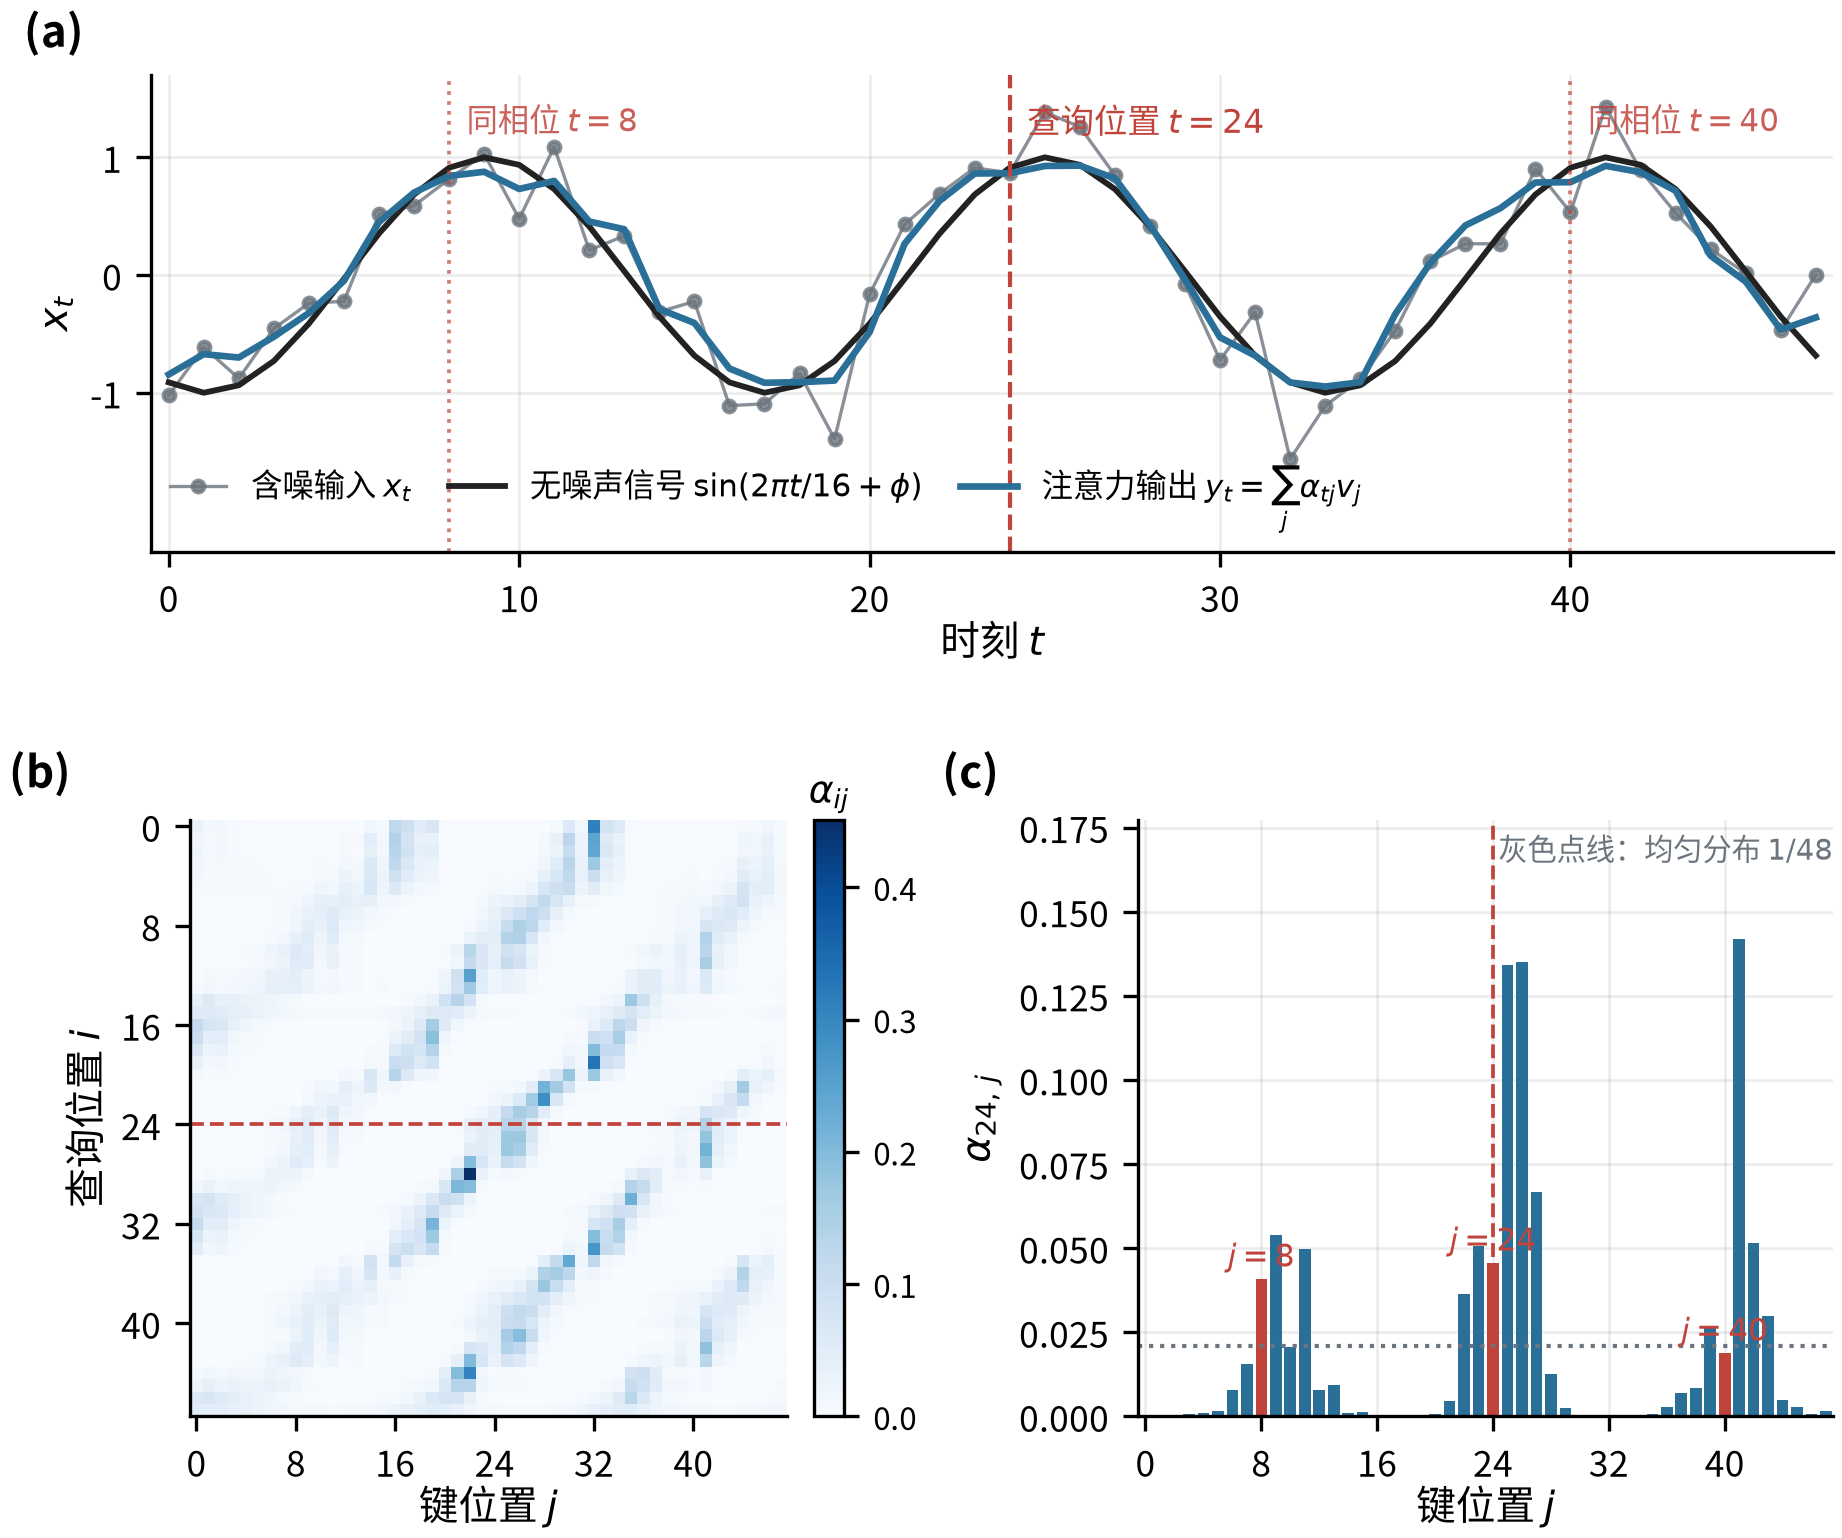
\includegraphics[width=0.98\textwidth]{figs_chap11/chap11_fig1.png}
\caption{一个真实训练出来的单头自注意力（\texttt{code\_chap11/chap11\_figures.py}）：输入是含噪的正弦序列 $x_t=\sin(2\pi t/16+\phi)+\varepsilon_t$（$T=48$，三个周期），$Q,K,V$ 由最近 4 个采样值线性映射得到，训练目标是还原无噪声的信号。（a）含噪输入（灰点）、真实信号（黑线）与注意力输出（蓝线）：输出的均方误差约为输入噪声的一半。（b）注意力矩阵 $\alpha_{ij}=\mathrm{softmax}_j(q_i\cdot k_j/\sqrt{d_k})$：平行于对角线、间距为 16 的条纹说明模型学会了``关注相位相同的时刻''。（c）查询位置 $t=24$ 的注意力分布：权重集中在 $j\approx 8,24,40$ 三簇（合计约 0.95），其余位置几乎为零——注意力就是按相似度加权的平均，即正文所说的 softmax 核回归。}
\label{fig:chap11_attention}
\end{figure}

\begin{figure}[htbp]
\centering
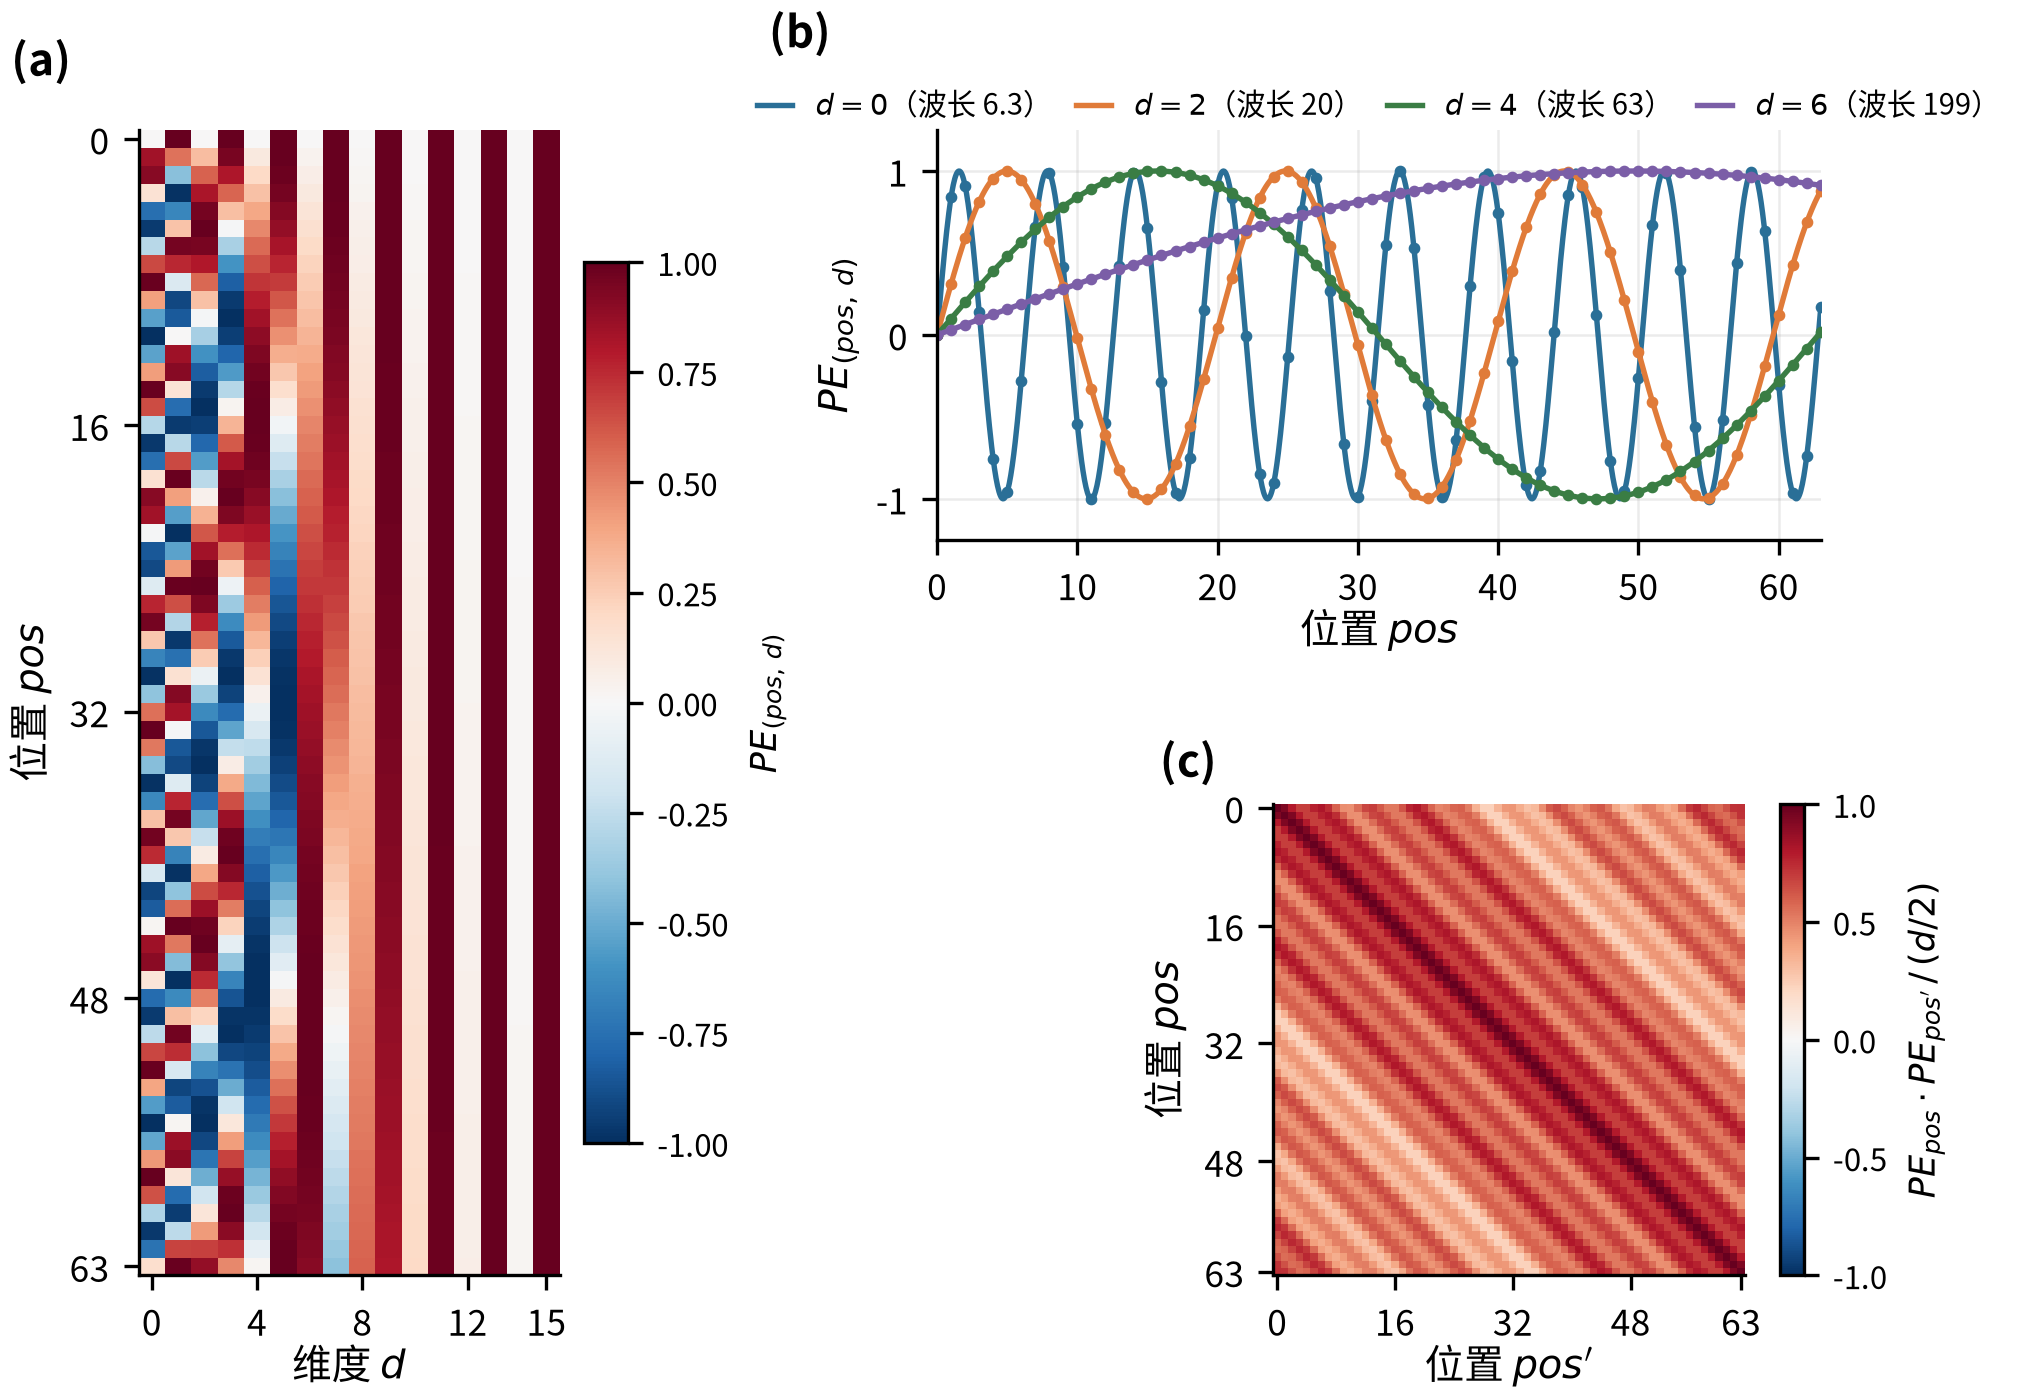
\includegraphics[width=0.95\textwidth]{figs_chap11/chap11_fig2.png}
\caption{正弦位置编码（$d_{\text{model}}=16$，位置 $0\sim 63$）。（a）编码矩阵 $PE_{(pos,d)}$：低维度变化快（高频），高维度变化慢（低频），最右几列在 64 个位置内几乎不变。（b）维度 $0,2,4,6$ 的正弦分量，波长分别为 $6.3,20,63,199$：一个位置的编码就是一组不同频率的``时钟指针''。（c）位置之间的归一化点积 $PE_{pos}\cdot PE_{pos'}/(d/2)$：矩阵沿对角线平移不变，只依赖相对位置 $pos-pos'$，相邻位置最相似——这正是``$PE_{pos+k}$ 是 $PE_{pos}$ 的线性变换''的体现。}
\label{fig:chap11_positional_encoding}
\end{figure}


% ====================================================================================
\section{视觉--语言模型：把图像也变成 token}
% ====================================================================================

到目前为止，本章的 Transformer 只吃一种东西：文本 token。可是物理智能要面对的世界不是一串字，而是一张张图像、一段段视频。让语言模型“睁开眼睛”的办法，出人意料地简单：\textbf{不改 Transformer，改输入}——把图像也变成一串 token，和文本 token 拼在同一条序列里，剩下的交给注意力。本节沿着这条思路走一遍：图像怎么切成 token，视觉编码器怎么训，怎么接到语言模型上，以及整套系统按什么配方训练。每一步我们照例问同样的三个问题：目标是什么、约束是什么、$\lambda$ 代表什么。

% ------------------------------------------------------------------------------------
\subsection{为什么要把图像变成 token}
% ------------------------------------------------------------------------------------

回顾本章“注意力机制”一节：注意力只做一件事——对一组向量按相似度做加权平均。它不关心这些向量从哪里来，是一个词、一个像素块，还是一段声音。这意味着 Transformer 天然是一个\textbf{与模态无关}的机器：只要你能把任何信号表示成“一串 $d$ 维向量”，它就能处理。

\begin{keyidea}[感知的统一接口]
Transformer 只认一种输入：形状为 $T \times d$ 的向量序列。因此，让模型“看见”的问题，就被转化为一个\textbf{接口问题}：
\begin{equation}
    \text{图像} \;\xrightarrow{\;\text{某种编码器}\;}\; X_{\text{img}} \in \mathbb{R}^{N \times d}, \qquad
    \text{文本} \;\xrightarrow{\;\text{分词 + 嵌入}\;}\; X_{\text{txt}} \in \mathbb{R}^{T \times d},
\end{equation}
然后把两者拼成一条长度为 $N + T$ 的序列送进同一个 Transformer。文本、图像、音频、机器人的关节角度，在这个接口之后都是一样的东西——token。
\end{keyidea}

这个想法之所以重要，是因为它把“多模态”从一个架构问题变成了一个\textbf{表示问题}：我们不需要为每种感官设计一套新的网络，只需要为每种感官设计一个“翻译成 token”的前端。

% ------------------------------------------------------------------------------------
\subsection{ViT：把图片切成 patch}
% ------------------------------------------------------------------------------------

一张 $224 \times 224$ 的彩色图像有 $224 \times 224 \times 3 \approx 150{,}000$ 个数。如果把每个像素当一个 token，序列长度 $T = 50{,}176$，注意力的 $O(T^2)$ 代价会立刻把我们压垮。视觉 Transformer（Vision Transformer, ViT，2020）的解法是：不看像素，看\textbf{小块}（patch）。
\storynote{Alexey Dosovitskiy}{2020 年，Google 的 Dosovitskiy 等人发表《An Image Is Worth 16x16 Words》。标题就是全部思想：一张图等于 196 个“单词”。当时很多人认为卷积的归纳偏置不可替代，而这篇论文表明，只要数据够多，一个几乎没改动的文本 Transformer 也能在图像分类上追平甚至超过卷积网络。}

\paragraph{patch 化}

把图像切成互不重叠的 $P \times P$ 小块。对 $224 \times 224$ 的图，取 $P = 16$ 时每边 $224/16 = 14$ 块，共 $14^2 = 196$ 个 patch；取 $P = 14$ 时每边 $224/14 = 16$ 块，共 $16^2 = 256$ 个 patch。每个 patch 展平后是一个 $P^2 \cdot 3$ 维的向量（$P = 16$ 时是 768 维）。于是一张图从“$150{,}000$ 个像素”变成了“196 个 768 维向量”——序列长度降到了和一段文本差不多的量级。

\paragraph{线性嵌入与位置编码}

接下来的步骤和本章“文本到数字”一节完全平行：
\begin{equation}
    z_i = W_{\text{patch}}\, \mathrm{vec}(\text{patch}_i) + p_i, \qquad i = 1, \dots, N,
\end{equation}
其中 $W_{\text{patch}} \in \mathbb{R}^{d \times 3P^2}$ 是一个线性层（相当于文本的“查词表”，只不过这里是乘一个矩阵而不是查一行），$p_i$ 是位置编码。位置编码在这里更加不可或缺：注意力本身不知道两个 patch 谁在左谁在右、谁在上谁在下，把 196 个 patch 打乱顺序它也看不出来。ViT 用的是可学习的位置编码，把二维网格按行展开成一维序号即可；也有工作显式地用二维坐标构造编码。

\paragraph{汇聚：[CLS] 还是均值}

经过 $L$ 层 Transformer 后，我们得到 $N$ 个输出向量。如果任务需要“整张图的一个向量”（例如分类或者和一句话做对比），有两种常见做法：在序列前面多加一个可学习的特殊 token \texttt{[CLS]}，让它通过注意力从所有 patch 里“收集”信息，取它的输出；或者干脆对 $N$ 个输出向量取平均（均值池化）。两者效果通常相近。

\paragraph{和文本 token 的三点不同}

第一是\textbf{连续与离散}之别：文本 token 是词表里的整数 ID，图像 patch 是连续向量。这意味着图像 token 没有“词表”，也就没法像文本那样用 softmax 交叉熵去“预测下一个 patch”——这一点在后面讨论训练损失时会再回来。第二是\textbf{序列长度}：一句话通常几十个 token，而一张 $224 \times 224$ 的图是 196 或 256 个；分辨率翻倍，patch 数翻四倍。图像是“话多”的模态。第三是\textbf{信息密度}：一个词几乎每个都有意义，而相邻的 patch 高度冗余（一片蓝天切出的几十个 patch 几乎一样）。这为后面的“压缩”留下了空间。

% ------------------------------------------------------------------------------------
\subsection{视觉编码器怎么训：对比学习}
% ------------------------------------------------------------------------------------

ViT 只是一个架构，它输出的向量有没有“意义”，取决于用什么目标去训它。最早的 ViT 用图像分类标签训练——这条路线的数据基础是李飞飞团队 2009 年发布的 ImageNet，它的标注是靠亚马逊 Mechanical Turk 众包完成的。而今天视觉--语言模型里的视觉编码器，几乎都用\textbf{图文对比学习}（contrastive learning）训练，代表是 CLIP（2021）和 SigLIP（2023）。

想法很直接：互联网上有海量“图片 + 文字说明”的配对——Radford 等人 2021 年发布的 CLIP 就用了 4 亿对。我们训练一个图像编码器 $f$ 和一个文本编码器 $g$，让配对的图和文在同一个向量空间里靠近，不配对的远离。取一个批次的 $B$ 个图文对，把编码后的向量归一化到单位球面上：$u_i = f(\text{img}_i)/\|f(\text{img}_i)\|$，$v_j = g(\text{txt}_j)/\|g(\text{txt}_j)\|$，相似度就是内积 $s_{ij} = u_i^\top v_j \in [-1, 1]$。

\begin{keyformula}[title=CLIP 的对比损失]
对第 $i$ 张图，在 $B$ 段文本里“选出”它的配文，这是一个 $B$ 类分类问题：
\begin{equation}
    p_{ij} = \frac{\exp(s_{ij}/\tau)}{\sum_{k=1}^{B} \exp(s_{ik}/\tau)}, \qquad
    \ell_{\text{img}\to\text{txt}} = -\frac{1}{B}\sum_{i=1}^{B} \log p_{ii}.
    \label{eq:clip_loss}
\end{equation}
对称地再做一遍“文找图”，两者取平均就是 CLIP 的损失。$\tau$ 是温度。把 $-\log p_{ii}$ 展开，每一项都可以拆成两部分：
\begin{equation}
    -\log p_{ii} = -\frac{s_{ii}}{\tau} + \log \sum_{k=1}^{B} e^{s_{ik}/\tau}.
    \label{eq:clip_split}
\end{equation}
\end{keyformula}

式~\eqref{eq:clip_split} 的拆分值得多看一眼：第一项把匹配对的相似度\textbf{往上拉}，第二项是配分函数的对数，把所有对的相似度\textbf{往下压}。这正是第4章的结构——$p_{ij}$ 是一个玻尔兹曼分布，$\log\sum_k e^{s_{ik}/\tau}$ 就是 $\log Z$。
\review{第4章}{在给定“期望相似度”约束下最大化熵，解是 $p_{ij} \propto \exp(\beta s_{ij})$，$\beta$ 是这条约束的拉格朗日乘子。对比学习里的 $1/\tau$ 就是这个 $\beta$：温度是乘子的倒数。这和本章注意力里的 $1/\sqrt{d_k}$ 是同一个角色。}

\begin{keyidea}[对比学习的目标 / 约束 / $\lambda$]
\textbf{目标}是最大化匹配对的对数似然 $\sum_i \log p_{ii}$，等价于让 $u_i$ 和 $v_i$ 的内积在所有候选中脱颖而出。\textbf{约束}有两条。第一条是 $u_i, v_j$ 落在单位球面上，$\|u_i\| = \|v_j\| = 1$：没有它，模型只要把向量的模长放大就能让 $\log Z$ 项随意变化，“相似”就失去了意义；归一化是这条约束的硬性实现。第二条是每张图对 $B$ 段文本的“注意力” $p_{i\cdot}$ 必须是一个概率分布——归一化约束，它的乘子给出 $\log Z$，也就是式~\eqref{eq:clip_split} 的第二项。而 \textbf{$\lambda$} 就是 $1/\tau$，即“期望相似度”约束的乘子：$\tau$ 越小，分布越尖，模型越“确信”；$\tau$ 越大，分布越平，匹配与不匹配的差别被抹平。CLIP 干脆把 $\tau$ 也设成可学习参数（初始值 $0.07$）——让模型自己决定这条约束的价格。
\end{keyidea}

SigLIP 做了一个小而重要的改动：不再要求 $p_{i\cdot}$ 在整个批次上归一化，而是对每一对 $(i, j)$ 独立地做一个二分类——“这一对是不是配对的”——用 sigmoid 损失。这去掉了上面的第二条约束，于是不再需要全批次的 $\log Z$，损失可以按对拆开计算，对 batch 大小的依赖也小得多。在本书的语言里，这是把一条全局归一化约束换成了 $B^2$ 条相互独立的局部约束。

训练好之后，我们只保留图像编码器 $f$（通常连 \texttt{[CLS]} 之前的 $N$ 个 patch 输出一起保留），它的输出向量已经“知道”哪些视觉特征对应哪些词——这是把它接到语言模型上的最好起点。

% ------------------------------------------------------------------------------------
\subsection{接到语言模型上：连接器与多模态序列}
% ------------------------------------------------------------------------------------

\begin{figure}[htbp]
\centering
\begin{tikzpicture}[>=stealth, scale=0.88, every node/.style={transform shape},
    block/.style={draw, rounded corners, minimum width=2.5cm, minimum height=0.95cm, align=center, font=\small}]
    % 第一行：图像通路
    \node[block, fill=blue!20] (img) at (0, 2.4) {图像\\$H \times W \times 3$};
    \node[block, fill=blue!20] (patch) at (3.4, 2.4) {切成 patch\\$N$ 个 $P \times P$ 小块};
    \node[block, fill=green!20] (vit) at (6.8, 2.4) {视觉编码器\\(ViT)};
    \node[block, fill=orange!20] (conn) at (10.2, 2.4) {连接器\\投影 / 重采样};
    % 第二行：文本通路与拼接
    \node[block, fill=blue!20] (txt) at (0, 0) {文本提示\\``图里是什么''};
    \node[block, fill=green!20] (emb) at (3.4, 0) {分词 + 嵌入\\$T$ 个文本 token};
    \node[block, fill=purple!20] (cat) at (6.8, 0) {拼接成一条序列\\$N' + T$ 个 token};
    % 第三行：语言模型与输出
    \node[block, fill=red!20] (llm) at (6.8, -2.4) {语言模型\\(Transformer 解码器)};
    \node[block, fill=green!20] (out) at (10.2, -2.4) {输出文本\\逐 token 生成};
    % 箭头
    \draw[->, thick] (img) -- (patch);
    \draw[->, thick] (patch) -- (vit);
    \draw[->, thick] (vit) -- node[above, font=\scriptsize] {$N$ 个向量} (conn);
    \draw[->, thick] (conn.south) |- node[pos=0.75, above, font=\scriptsize] {$N'$ 个视觉 token} (cat.east);
    \draw[->, thick] (txt) -- (emb);
    \draw[->, thick] (emb) -- (cat);
    \draw[->, thick] (cat) -- (llm);
    \draw[->, thick] (llm) -- (out);
    % 标注
    \node[below, font=\scriptsize, gray, align=center] at (3.4, -2.4) {损失只算输出文本的\\下一词预测};
\end{tikzpicture}
\caption{视觉--语言模型的数据流：图像切成 patch，经视觉编码器得到 $N$ 个向量，再由连接器变成 $N'$ 个和文本嵌入同维度的视觉 token（$N' \le N$），与文本 token 拼成一条序列送进语言模型。语言模型本身不需要为图像做任何改动。}
\label{fig:vlm_pipeline}
\end{figure}

视觉编码器输出的向量维度（例如 1024）一般和语言模型的嵌入维度（例如 4096）不一样，“语义坐标系”也不一样。中间需要一个\textbf{连接器}（connector），把视觉向量翻译成语言模型能读的 token。连接器有两种主流设计。

\paragraph{投影层：一个 patch 一个 token}

最简单的做法是一个线性层或两层 MLP：
\begin{equation}
    X_{\text{img}} = \mathrm{MLP}(Z_{\text{ViT}}) \in \mathbb{R}^{N \times d_{\text{LLM}}}.
\end{equation}
LLaVA（2023）就是这么做的：CLIP 的 ViT-L/14 编码器，接一个投影层，直接把每个 patch 变成一个 token。在 $336 \times 336$ 分辨率、$P = 14$ 下，一张图就是 $24^2 = 576$ 个 token。它的优点是不丢信息、不引入新的注意力模块；缺点是 token 多。

\paragraph{重采样：把几百个压成几十个}

另一种做法利用前面提到的冗余：用 $K$ 个\textbf{可学习的查询向量}（$K$ 远小于 $N$）对 $N$ 个 patch 做交叉注意力，把信息“吸”进 $K$ 个 token 里。Flamingo（2022）的 Perceiver Resampler 用 64 个查询，BLIP-2（2023）的 Q-Former 用 32 个。这正是本章注意力的另一种用法：查询 $Q$ 不再来自输入本身，而是一组学出来的“提问”，$K, V$ 来自 patch。序列从几百压到几十，代价是压缩必然有损，细小的文字、远处的物体可能被“平均掉”。

也有人干脆跳过视觉编码器，把 patch 线性投影后直接喂进语言模型（Fuyu，2023）。这把“感知的统一接口”贯彻到了极致，代价是语言模型必须从零学会看图，需要多得多的图像数据。

\paragraph{图文交错序列}

连接器输出的视觉 token 和文本 token 处于同一个空间，于是可以像文字一样自由排布：
\begin{center}
\texttt{<image>}$\;\underbrace{x_1 \cdots x_{N'}}_{\text{视觉 token}}\;$\texttt{</image>} 这张图里有几只猫？\texttt{<assistant>} 两只。
\end{center}
一段对话里可以有多张图、图和文交替出现，模型统统当成一条序列来处理。图像的“位置”就是它在序列中的位置——位置编码对视觉 token 照常生效。

\paragraph{注意力掩码：文本因果，图像双向}

本章“只用 Decoder”一节里，GPT 用因果掩码禁止每个 token 看到未来。对视觉 token，这个限制没有道理：一张图的左上角 patch 完全可以“看”右下角，图像内部没有先后。PaliGemma（2024）采用的 \textbf{prefix-LM} 掩码把这一点写得很清楚：把图像 token 和用户提示当作“前缀”，前缀内部\textbf{双向}注意力，只有模型要生成的“后缀”才用因果掩码。用 $\mathcal{P}$ 记前缀的位置集合，掩码可以写成
\begin{equation}
    M_{ij} =
    \begin{cases}
        1, & j \le i \quad \text{（因果：可以看过去）} \\
        1, & i \in \mathcal{P} \text{ 且 } j \in \mathcal{P} \quad \text{（前缀内部：可以互看）} \\
        0, & \text{其他}
    \end{cases}
\end{equation}
$M_{ij} = 0$ 的位置在 softmax 之前被置为 $-\infty$。这个掩码和本章 Encoder-Decoder 结构的精神一致：前缀相当于一个“编码器”，只不过它和解码器共用同一套参数。

\paragraph{高分辨率的代价：token 数暴涨}

$224 \times 224$ 看不清发票上的小字。提高分辨率最直接的办法是\textbf{切块}：把一张大图切成若干个 $336 \times 336$ 的子块，每块单独过一遍编码器，再加上一张缩小的全局缩略图。四个子块加一张缩略图，就是 $5 \times 576 = 2{,}880$ 个 token——一张图的 token 数已经超过一篇短文。视频更甚：每秒抽几帧，每帧几百个 token，一分钟视频轻松上万。
\preview{视觉 token 直接进入 KV Cache：每层每个 token 都要存一份 $K$ 和 $V$。一张高分辨率图的 2{,}880 个 token 占的显存，和 2{,}880 个文字 token 一模一样。附录C会给出可以直接套用的估算公式，并讨论显存作为一条硬约束时，它的影子价格如何决定“该不该压缩视觉 token”。}

这就是为什么“重采样压缩”和“按需分辨率”成了工程上的核心问题：视觉 token 不是免费的，它们和文本 token 一样要占 $O(T^2)$ 的注意力算力与线性增长的 KV Cache。

% ------------------------------------------------------------------------------------
\subsection{和 LLM 一起训练的三阶段配方}
% ------------------------------------------------------------------------------------

现在三个部件齐了：预训练好的视觉编码器、随机初始化的连接器、预训练好的语言模型。怎么把它们训成一个整体？当前主流配方分三个阶段。

\paragraph{阶段一：对齐预训练}

冻结视觉编码器和语言模型，\textbf{只训连接器}。数据是大量简单的图文对（一张图、一句描述），任务是“看图写说明”。这一阶段的目的很单纯：让连接器学会把视觉向量翻译成语言模型“听得懂”的 token。

\paragraph{阶段二：指令微调}

解冻语言模型（有些配方也解冻视觉编码器，但用小得多的学习率），在高质量的多模态指令数据上训练：看图问答、看图推理、多轮对话、读图表、识别文档。同时\textbf{混入一定比例的纯文本指令数据}。这一阶段模型才真正学会“按要求看图做事”。

\paragraph{阶段三：偏好对齐}

和纯文本大模型一样，最后用人类偏好数据做强化学习或直接偏好优化，重点压制多模态特有的问题——例如“幻觉”：描述图里根本不存在的物体。本书不展开这一阶段，其原理见第9章。

\paragraph{损失函数：只算文本}

三个阶段用的都是本章的下一词预测损失，但有一个关键细节：\textbf{图像 token 不预测}。设序列为 $x_1, \dots, x_{N'+T}$，用掩码 $m_t \in \{0, 1\}$ 标出需要预测的位置（只有模型应当生成的文本 token 为 1），
\begin{equation}
    \ell(\theta) = -\sum_{t} m_t \log p_\theta(x_t \mid x_{<t}).
\end{equation}
原因有两个：一是视觉 token 是连续向量，没有词表可供分类；二是在 prefix-LM 掩码下前缀内部可以互看，“预测”前缀里的 token 等于作弊。图像在这里只是\textbf{条件}，不是\textbf{目标}。
\clarify{“冻结”一个模块的意思是不更新它的参数，而\textbf{不是}不经过它反向传播。阶段一里语言模型虽然被冻结，伴随变量 $\lambda$（第8章的误差信号）仍然要从损失出发穿过整个语言模型，才能到达连接器。冻结省的是优化器状态和参数更新，不省反向传播的算力。}

\paragraph{为什么要分阶段？为什么要混纯文本？}

用本书的框架来看，这两条经验都不是“技巧”，而是一条约束的两种处理方式。

\begin{keyidea}[多模态训练的目标 / 约束 / $\lambda$]
\textbf{目标}是多模态数据上的下一词预测损失 $\ell_{\text{mm}}(\theta)$——学会看图。\textbf{约束}是语言模型原有的语言能力不能退化，写成不等式就是 $\ell_{\text{txt}}(\theta) \le \ell_{\text{txt}}(\theta_0) + \epsilon$，其中 $\theta_0$ 是预训练语言模型的参数，$\ell_{\text{txt}}$ 是纯文本数据上的损失；或者写成 $\mathrm{KL}\big(p_\theta \,\|\, p_{\theta_0}\big) \le \epsilon$。于是\textbf{拉格朗日函数}为
\begin{equation}
    \mathcal{L}(\theta, \lambda) = \ell_{\text{mm}}(\theta) + \lambda \big[\ell_{\text{txt}}(\theta) - \ell_{\text{txt}}(\theta_0) - \epsilon\big].
\end{equation}
这里的 \textbf{$\lambda$} 就是训练数据里\textbf{纯文本数据的混合比例}（或 KL 正则项的系数）。它是“不遗忘”这条约束的影子价格：把语言能力的门槛 $\epsilon$ 放松一点，多模态损失能降多少。
\end{keyidea}

有了这个视角，三阶段配方就顺理成章了。\textbf{阶段一是把约束当硬约束}：$\theta_{\text{LLM}} \equiv \theta_0$，语言能力\textbf{不可能}退化。此时连接器是随机初始化的，它送进语言模型的是一堆噪声；如果这时就放开语言模型的参数，梯度会为了“迁就噪声”把语言能力冲垮——这条约束的影子价格在此刻极高，硬约束是最便宜的处理方式。

\textbf{阶段二把硬约束换成软约束}：连接器对齐之后，视觉 token 已经“像话”了，进一步提升需要语言模型本身配合，约束的影子价格降下来，于是可以解冻。混入纯文本数据就是显式地把 $\lambda\,\ell_{\text{txt}}$ 这一项加进损失；给编码器一个更小的学习率，则是对“不要偏离 $\theta_0$”这条约束的另一种软化——每一步只允许在原参数附近的一个小邻域里移动。

\textbf{混合比例不是拍脑袋定的}：按第1章互补松弛的读法，$\lambda$ 应当由约束是否被激活来决定。实际操作中人们会监控纯文本基准的分数：分数掉了，说明约束被违反，就该调高纯文本比例——这正是“按影子价格调乘子”的手工版本。

\begin{physicalmeaning}[title=$\lambda$ 在视觉--语言模型里的两种身份]
本节出现了两个 $\lambda$，它们在同一个框架里扮演不同角色。对比学习里的 $1/\tau$ 是一个“分布层面”的乘子，决定图文匹配分布的尖锐程度，与第4章的逆温度、本章注意力的 $1/\sqrt{d_k}$ 同源；它对应的约束是“期望相似度”，是关于\textbf{单个样本内部}的约束。训练配方里的混合比例则是一个“参数层面”的乘子，决定新能力（看图）与旧能力（说话）之间的交换率；它对应的约束是“不遗忘”，是关于\textbf{整个模型}的约束。两者都回答同一个问题：把约束松一点，目标能好多少。
\end{physicalmeaning}

% ------------------------------------------------------------------------------------
\subsection{从看图说话到看图做事}
% ------------------------------------------------------------------------------------

到这里，语言模型已经能看图、答题、描述场景。但物理智能要的不止于此：机器人看到桌上的杯子，需要的不是一句“桌上有个杯子”，而是一串关节角度。

沿着本节的思路，答案几乎是自动的。既然图像可以变成 token 拼进序列，动作为什么不能？把机器人的动作离散化成词表里的整数，让语言模型像生成文字一样生成动作 token，这是一条路；保留语言模型不动，在旁边接一个专门输出连续动作的“动作专家”，用视觉--语言模型的隐状态作为它的条件，这是另一条路。两条路都建立在同一个基础上：一个已经对齐了视觉和语言的骨干网络。
\preview{第17章讨论具身智能时会回到这里：视觉--语言--动作模型（VLA）把本节的视觉--语言模型当作骨干，再加上动作输出——例如 $\pi_0$（2024）就以 PaliGemma 为骨干，外接一个用流匹配训练的动作专家。到那时你会看到，“动作也是 token”这句话背后，仍然是同一个 $\mathcal{L} = f + \lambda^\top g$：目标是任务成功，约束是物理可行与安全，$\lambda$ 是安全的价格。}

\begin{insightbox}[title=统一接口，再看一次]
本章的故事绕了一个圈又回到起点：Transformer 之所以能成为物理智能的骨干，不是因为它“懂语言”，而是因为它提供了一个统一的接口——任何能被写成 token 序列的东西，它都能建模。视觉--语言模型没有给 Transformer 增加任何新机制，只是在接口前面多加了一个“图像到 token”的翻译器，再用一条“不遗忘”约束把新旧能力捆在一起。任何能被写成 $\mathcal{L} = f + \lambda^\top g$ 的东西，我们都能用同一套语言读懂它的设计。
\end{insightbox}

% ====================================================================================
\section{本章小结}
% ====================================================================================

\subsection{核心要点}
\preview{会看、会说之后怎么变成会做事？第12章讲后训练：奖励是目标、参考模型是约束、RLHF 的 $\beta$ 就是 $\lambda$；第17章再把本章的 VLM 接上动作。}

\begin{enumerate}
    \item \textbf{RNN的问题}：参数共享导致梯度连乘，信息瓶颈导致长距离依赖丢失
    
    \item \textbf{LSTM的缓解}：门控机制让梯度可以“直通”，但仍是串行计算
    
    \item \textbf{Transformer的解决}：用注意力实现全连接，路径长度 $O(1)$；每层参数不同，避免连乘同一矩阵；可并行计算，代价是 $O(T^2)$ 复杂度
    
    \item \textbf{Q、K、V的来源}：同一输入通过三个不同的线性变换得到
    
    \item \textbf{多头注意力}：让模型从多个角度关注序列
    
    \item \textbf{视觉--语言模型}：把图像切成 patch、编码成向量、经连接器变成 token，与文本 token 拼成一条序列送进同一个 Transformer；对比学习的温度 $1/\tau$ 与训练配方里的纯文本混合比例，是“期望相似度”与“不遗忘”两条约束的乘子
\end{enumerate}

\begin{physicalmeaning}[title=$\lambda_t$ 在本章的意义]
$\lambda_t$ 是第 $t$ 步隐状态的\textbf{影子价格}：把递推约束 $h_{t+1} = F(h_t, x_t)$ 松开一点、让 $h_t$ 多偏 $\delta$，总损失变化 $\lambda_t^\top \delta$。本章的几个主角都可以用它来读。\textbf{梯度消失}就是早期状态的影子价格趋于零：$\lambda_0 \approx (\prod_t J_t)^\top \lambda_T \to 0$，优化器“看不见”早期信息的价值。\textbf{LSTM 的遗忘门} $f_t \approx 1$ 让 $\partial c_t/\partial c_{t-1} \approx I$，影子价格不折价地往回传。\textbf{Transformer 的残差流} $H^{(\ell+1)} = H^{(\ell)} + f_\ell(H^{(\ell)})$ 给出伴随 $\lambda^{(\ell)} = (I + \partial f_\ell)^\top \lambda^{(\ell+1)} \approx \lambda^{(\ell+1)}$，而且只有 $L$ 层而不是 $T$ 步。本章还有\textbf{第二个 $\lambda$}：注意力权重 $\mathrm{softmax}(q^\top k/\sqrt{d_k})$ 是第4章最大熵问题的解，$1/\sqrt{d_k}$ 就是“期望相似度”约束的乘子——温度的倒数。
\end{physicalmeaning}

\begin{unification}[title=统一视角]
第7章的协态、第8章的误差信号 $\lambda_i$、第9章的伴随变量 $\lambda_t$、本章的 BPTT 梯度 $\partial J/\partial h_t$，是同一个对象：动力学约束的拉格朗日乘子。附录C会问一个更工程的问题：当这 $T$ 条约束占用的显存与算力本身成为约束时，它们的影子价格是多少？
\end{unification}


\begin{table}[htbp]
\centering
\renewcommand{\arraystretch}{1.4}
\begin{tabularx}{\textwidth}{p{2.2cm}|X|X|X}
\toprule
& \textbf{RNN} & \textbf{LSTM} & \textbf{Transformer} \\
\midrule
\textbf{信息流} & 串行链式 & 串行 + 高速公路 & 全连接 \\
\textbf{梯度路径} & $O(T)$ 连乘 & $O(T)$ 但可直通 & $O(1)$ 直连 \\
\textbf{并行性} & 不可并行 & 不可并行 & 完全并行 \\
\textbf{复杂度} & $O(T)$ & $O(T)$ & $O(T^2)$ \\
\textbf{长距离依赖} & 困难 & 较好 & 优秀 \\
\bottomrule
\end{tabularx}
\caption{三种序列模型的对比}
\end{table}

% ====================================================================================
\section{习题}
% ====================================================================================

\paragraph{计算题}
\begin{enumerate}
    \item 设RNN的权重矩阵 $W_h$ 的特征值为 $\mu_1 = 0.95, \mu_2 = 0.85$。计算经过 $T = 50$ 步后，沿最大特征向量方向的梯度衰减倍数。
    
    \item 在一个注意力头中，$d_k = 64$。假设Q和K的每个元素独立服从 $\mathcal{N}(0, 1)$，计算点积 $q \cdot k$ 的标准差。解释为什么要除以 $\sqrt{d_k}$。
    
    \item 计算自注意力的时间和空间复杂度。设序列长度为 $T$，嵌入维度为 $d$，头数为 $h$。
    
    \item 一个Transformer模型有 $L = 32$ 层，$d = 4096$，$h = 32$ 头。计算KV Cache在处理长度 $T = 8192$ 的序列时占用的显存（假设使用float16）。
\end{enumerate}

\paragraph{编程题}
\begin{enumerate}
    \setcounter{enumi}{4}
    \item 用 NumPy 手算一个 3 个 token、$d_k = 2$ 的自注意力：自己给定 $Q, K, V$，算出注意力权重矩阵和输出，再用 PyTorch 的 \texttt{torch.nn.functional.}\allowbreak\texttt{scaled\_dot\_product\_attention} 验证。
    
    \item 用 PyTorch 实现一个简化版 \texttt{TransformerBlock}（Pre-Norm：多头注意力 + 前馈网络 + 残差 + LayerNorm，约 40 行）；用 \texttt{torch.autograd.}\allowbreak\texttt{gradcheck} 检查梯度，并在一个字符级语言建模玩具任务上训练几百步。
\end{enumerate}

\paragraph{思考题}
\begin{enumerate}
    \setcounter{enumi}{6}
    \item 解释为什么RNN的梯度会消失或爆炸。用特征值的语言描述。
    
    \item 数据处理不等式如何限制了RNN的长距离建模能力？
    
    \item 为什么Transformer的残差连接有助于梯度传播？从伴随方程的角度解释。
    
    \item 解释Q、K、V的含义，以及为什么需要三个不同的投影矩阵。
    
    \item 多头注意力相比单头注意力有什么优势？为什么每个头的维度要缩小？
    
    \item LSTM的遗忘门 $f_t$ 接近1时可以缓解梯度消失，但为什么不能完全解决长距离依赖问题？从信息论角度思考。
    
    \item Transformer的 $O(T^2)$ 复杂度在处理超长序列时是瓶颈。你能想到什么方法来降低复杂度？（提示：稀疏注意力、线性注意力）
    
    \item 为什么GPT只用Decoder而BERT只用Encoder？它们的训练目标有什么不同？
    
    \item 从第一性原理角度，注意力机制可以看作是基于最大熵原则的软检索。这与传统的硬检索（如数据库查询）有什么本质区别？
    
    \item 一个视觉--语言模型在阶段二解冻了语言模型，训练后看图能力提升，但纯文本基准分数明显下降。用本章“目标 / 约束 / $\lambda$”的语言描述发生了什么：哪条约束被违反了？对应的乘子是训练配方里的哪个量？给出两种把这个乘子“调高”的具体做法，并说明各自的代价（提示：一种改数据，一种改损失函数；再想想它们对显存和训练时间的影响）。
\end{enumerate}
  % 第11章：序列建模：从RNN到Transformer
% ====================================================================================
\chapter{Transformer实战：显存、算力与工程实现}
% ====================================================================================

\section*{引言：从论文到实验室}

\marginnote{本章内容是你在实验室跑实验必须具备的"工程直觉"。不懂这些，代码写对了也跑不起来。}

在前面的章节中，我们深入理解了Transformer的数学原理。但当你真正要在实验室训练或部署模型时，会遇到一系列非常实际的问题：

\begin{itemize}
    \item "导师给了我一个7B的模型，实验室的显卡能跑吗？"
    \item "为什么我的训练刚开始就报OOM（Out of Memory）？"
    \item "同学说他用4张卡，我只有2张，我的实验要跑多久？"
\end{itemize}

这些问题的答案需要你具备\textbf{工程直觉}——能够快速估算显存、预测训练时间、写出正确的代码。

本章分为四个部分：
\begin{enumerate}
    \item \textbf{硬件基础}：了解你手里的GPU能做什么
    \item \textbf{显存估算}：判断实验能不能跑起来
    \item \textbf{吞吐量计算}：预估实验要跑多久
    \item \textbf{代码实现}：手写核心组件
\end{enumerate}

% ====================================================================================
\section{认识你的GPU}
% ====================================================================================

\marginnote{\textbf{黄仁勋与NVIDIA}：NVIDIA创始人黄仁勋(Jensen Huang)是AI计算革命的关键人物。2006年推出CUDA让GPU可编程，2012年AlexNet用GPU训练催生深度学习浪潮，如今NVIDIA市值超2万亿美元。深度学习的成功很大程度上归功于GPU的并行计算能力。}

% ------------------------------------------------------------------------------------
\subsection{常见GPU参数速查}
% ------------------------------------------------------------------------------------

作为学生，你可能接触到以下几类GPU：

\begin{table}[h]
\centering
\small
\renewcommand{\arraystretch}{1.3}
\begin{tabular}{l|c|c|c|c|c}
\toprule
\textbf{型号} & \textbf{显存} & \textbf{FP16算力} & \textbf{显存带宽} & \textbf{功耗} & \textbf{定位} \\
\midrule
\multicolumn{6}{c}{\textit{消费级（个人/小实验室常见）}} \\
\midrule
RTX 3080 & 10 GB & 30 TFLOPS & 760 GB/s & 320W & 入门深度学习 \\
RTX 3090 & 24 GB & 36 TFLOPS & 936 GB/s & 350W & 个人炼丹主力 \\
RTX 4080 & 16 GB & 49 TFLOPS & 717 GB/s & 320W & 性价比之选 \\
RTX 4090 & 24 GB & 83 TFLOPS & 1008 GB/s & 450W & 消费级天花板 \\
\midrule
\multicolumn{6}{c}{\textit{专业级（实验室/计算中心常见）}} \\
\midrule
A100 40GB & 40 GB & 312 TFLOPS & 1555 GB/s & 400W & 主流科研卡 \\
A100 80GB & 80 GB & 312 TFLOPS & 2039 GB/s & 400W & 大模型训练 \\
H100 SXM & 80 GB & 990 TFLOPS & 3350 GB/s & 700W & 最新旗舰 \\
\midrule
\multicolumn{6}{c}{\textit{国产替代（部分高校可能接触）}} \\
\midrule
华为910B & 64 GB & 320 TFLOPS & 1200 GB/s & 400W & 国产主力 \\
\bottomrule
\end{tabular}
\caption{常见GPU参数对比（FP16/BF16算力，2024年数据）}
\end{table}

\marginnote{\textbf{TFLOPS}：每秒万亿次浮点运算。1 TFLOPS = $10^{12}$ FLOPS。这是衡量GPU计算能力的核心指标。}

\paragraph{几个关键概念}

\begin{itemize}
    \item \textbf{显存（VRAM）}：GPU的"内存"，决定能装多大的模型
    \item \textbf{算力（FLOPS）}：计算速度，决定训练/推理多快
    \item \textbf{显存带宽}：数据搬运速度，大模型推理的瓶颈往往在这里
    \item \textbf{功耗}：电费和散热的考量，实验室可能有限制
\end{itemize}

% ------------------------------------------------------------------------------------
\subsection{数据精度与存储}
% ------------------------------------------------------------------------------------

不同的数值精度决定了模型占用的显存大小：

\begin{table}[h]
\centering
\renewcommand{\arraystretch}{1.3}
\begin{tabular}{l|c|c|c|l}
\toprule
\textbf{精度} & \textbf{位数} & \textbf{字节} & \textbf{数值范围} & \textbf{典型用途} \\
\midrule
FP32 & 32 bit & 4 B & $\pm 3.4 \times 10^{38}$ & 传统训练、优化器状态 \\
TF32 & 19 bit & 4 B & 同FP32 & A100默认训练精度 \\
FP16 & 16 bit & 2 B & $\pm 6.5 \times 10^{4}$ & 混合精度训练 \\
BF16 & 16 bit & 2 B & $\pm 3.4 \times 10^{38}$ & 大模型训练（推荐） \\
INT8 & 8 bit & 1 B & $-128 \sim 127$ & 量化推理 \\
INT4 & 4 bit & 0.5 B & $-8 \sim 7$ & 激进量化 \\
\bottomrule
\end{tabular}
\caption{常见数值精度对比}
\end{table}

\begin{figure}[h]
\centering
\begin{tikzpicture}[scale=0.9]
    % FP32
    \node[font=\bfseries] at (-2, 2) {FP32:};
    \draw (0, 1.7) rectangle (0.8, 2.3);
    \node[font=\scriptsize] at (0.4, 2) {符号};
    \draw (0.8, 1.7) rectangle (3.2, 2.3);
    \node[font=\scriptsize] at (2, 2) {指数 (8位)};
    \draw (3.2, 1.7) rectangle (8, 2.3);
    \node[font=\scriptsize] at (5.6, 2) {尾数 (23位)};
    
    % FP16
    \node[font=\bfseries] at (-2, 1) {FP16:};
    \draw (0, 0.7) rectangle (0.5, 1.3);
    \node[font=\scriptsize] at (0.25, 1) {符};
    \draw (0.5, 0.7) rectangle (2, 1.3);
    \node[font=\scriptsize] at (1.25, 1) {指数 (5位)};
    \draw (2, 0.7) rectangle (5, 1.3);
    \node[font=\scriptsize] at (3.5, 1) {尾数 (10位)};
    
    % BF16
    \node[font=\bfseries] at (-2, 0) {BF16:};
    \draw (0, -0.3) rectangle (0.5, 0.3);
    \node[font=\scriptsize] at (0.25, 0) {符};
    \draw (0.5, -0.3) rectangle (2.9, 0.3);
    \node[font=\scriptsize] at (1.7, 0) {指数 (8位)};
    \draw (2.9, -0.3) rectangle (5, 0.3);
    \node[font=\scriptsize] at (3.95, 0) {尾数 (7位)};
    
    % 说明
    \node[right, font=\small, gray] at (8.5, 2) {精度最高，但慢且费显存};
    \node[right, font=\small, gray] at (5.5, 1) {容易溢出（范围小）};
    \node[right, font=\small, gray] at (5.5, 0) {范围大，精度够用（推荐）};
\end{tikzpicture}
\caption{不同浮点格式的位分配}
\end{figure}

\begin{keyidea}[BF16 vs FP16]
\begin{itemize}
    \item \textbf{FP16}：尾数多（精度高），但指数少（范围小），训练时容易溢出
    \item \textbf{BF16}：指数与FP32相同（范围大），尾数少但够用，训练更稳定
    \item \textbf{实践建议}：如果你的GPU支持BF16（A100、H100、RTX 30/40系列），优先用BF16
\end{itemize}
\end{keyidea}

% ====================================================================================
\section{显存估算：你的实验能跑吗？}
% ====================================================================================

显存是深度学习的"硬通货"。显存不够，代码写得再对也跑不起来。

% ------------------------------------------------------------------------------------
\subsection{模型参数的显存占用}
% ------------------------------------------------------------------------------------

\begin{keyformula}[title=模型显存速算]
\begin{equation}
    \text{模型显存 (GB)} = \text{参数量 (B)} \times \text{每参数字节数}
\end{equation}

速算口诀：
\begin{itemize}
    \item FP32：参数量 $\times$ 4
    \item FP16/BF16：参数量 $\times$ 2
    \item INT8：参数量 $\times$ 1
    \item INT4：参数量 $\times$ 0.5
\end{itemize}
\end{keyformula}

\begin{table}[h]
\centering
\renewcommand{\arraystretch}{1.3}
\begin{tabular}{l|c|c|c|c|c}
\toprule
\textbf{模型} & \textbf{参数量} & \textbf{FP32} & \textbf{FP16/BF16} & \textbf{INT8} & \textbf{INT4} \\
\midrule
GPT-2 & 1.5B & 6 GB & 3 GB & 1.5 GB & 0.75 GB \\
LLaMA-7B & 7B & 28 GB & 14 GB & 7 GB & 3.5 GB \\
LLaMA-13B & 13B & 52 GB & 26 GB & 13 GB & 6.5 GB \\
Qwen-14B & 14B & 56 GB & 28 GB & 14 GB & 7 GB \\
LLaMA-70B & 70B & 280 GB & 140 GB & 70 GB & 35 GB \\
\bottomrule
\end{tabular}
\caption{常见模型的参数显存需求（仅模型权重）}
\end{table}

\begin{example}[判断能否跑LLaMA-7B推理]
\textbf{场景}：实验室有一张RTX 3090（24GB），想跑LLaMA-7B推理。

\textbf{分析}：
\begin{itemize}
    \item FP16加载：$7 \times 2 = 14$ GB $\checkmark$ 可以
    \item 还剩 $24 - 14 = 10$ GB 给KV Cache和其他开销
    \item 结论：\textbf{可以跑}，但长文本生成时KV Cache可能爆显存
\end{itemize}

\textbf{如果只有RTX 3080（10GB）}：
\begin{itemize}
    \item FP16加载：14 GB > 10 GB $\times$ 跑不了
    \item INT4量化：$7 \times 0.5 = 3.5$ GB $\checkmark$ 可以
    \item 结论：必须用\textbf{4-bit量化}（如GPTQ、AWQ）
\end{itemize}
\end{example}

% ------------------------------------------------------------------------------------
\subsection{训练显存：为什么比推理大这么多？}
% ------------------------------------------------------------------------------------

新手常见困惑：为什么推理只要14GB，训练却要上百GB？

答案：训练需要存储的东西远不止模型权重。

\begin{figure}[h]
\centering
\begin{tikzpicture}[>=stealth, scale=0.85]
    % 推理
    \begin{scope}[xshift=-4.5cm]
        \node[font=\bfseries] at (1, 5.5) {推理};
        
        \draw[fill=blue!30] (0, 0) rectangle (2, 3);
        \node at (1, 1.5) {模型权重};
        \node[font=\small] at (1, 0.8) {14 GB};
        
        \draw[fill=gray!20] (0, 3) rectangle (2, 4);
        \node[font=\small] at (1, 3.5) {KV Cache};
        
        \draw[<->] (2.5, 0) -- (2.5, 4);
        \node[right, font=\small] at (2.5, 2) {$\approx$16 GB};
    \end{scope}
    
    % 训练
    \begin{scope}[xshift=3cm]
        \node[font=\bfseries] at (1.5, 5.5) {全量微调};
        
        \draw[fill=blue!30] (0, 0) rectangle (3, 1.5);
        \node at (1.5, 0.75) {模型权重 (FP16)};
        \node[font=\small, gray] at (1.5, 0.3) {14 GB};
        
        \draw[fill=green!30] (0, 1.5) rectangle (3, 3);
        \node at (1.5, 2.25) {梯度 (FP16)};
        \node[font=\small, gray] at (1.5, 1.8) {14 GB};
        
        \draw[fill=orange!30] (0, 3) rectangle (3, 6);
        \node at (1.5, 4.5) {优化器状态};
        \node[font=\small] at (1.5, 4) {(Adam, FP32)};
        \node[font=\small, gray] at (1.5, 3.5) {56 GB};
        
        \draw[fill=red!20] (0, 6) rectangle (3, 7.5);
        \node at (1.5, 6.75) {激活值};
        \node[font=\small, gray] at (1.5, 6.3) {可变};
        
        \draw[<->] (3.5, 0) -- (3.5, 6);
        \node[right, font=\small] at (3.5, 3) {$\geq$84 GB};
        \node[right, font=\scriptsize, red] at (3.5, 2.3) {一张A100都不够！};
    \end{scope}
\end{tikzpicture}
\caption{LLaMA-7B推理 vs 训练的显存对比}
\end{figure}

\paragraph{训练显存的四个组成部分}

\begin{enumerate}
    \item \textbf{模型权重}：和推理一样
    \begin{equation}
        M_{\text{weights}} = N \times \text{dtype\_size}
    \end{equation}
    
    \item \textbf{梯度}：每个参数对应一个梯度，大小与权重相同
    \begin{equation}
        M_{\text{gradients}} = N \times \text{dtype\_size}
    \end{equation}
    
    \item \textbf{优化器状态}：这是大头！以Adam为例：
    \begin{itemize}
        \item 一阶矩（Momentum）：$m_t = \beta_1 m_{t-1} + (1-\beta_1) g_t$
        \item 二阶矩（Variance）：$v_t = \beta_2 v_{t-1} + (1-\beta_2) g_t^2$
        \item 通常用FP32存储以保证数值稳定
    \end{itemize}
    \begin{equation}
        M_{\text{optimizer}} = N \times 2 \times 4 = 8N \quad \text{(Adam)}
    \end{equation}
    
    \item \textbf{激活值}：前向传播的中间结果，反向时要用
    \begin{itemize}
        \item 取决于Batch Size、序列长度、模型深度
        \item 可以用\textbf{梯度检查点}节省（用计算换显存）
    \end{itemize}
\end{enumerate}

\begin{keyformula}[title=全量微调显存估算]
\begin{equation}
    M_{\text{train}} \approx \underbrace{2N}_{\text{权重}} + \underbrace{2N}_{\text{梯度}} + \underbrace{8N}_{\text{优化器}} + M_{\text{激活}} = 12N + M_{\text{激活}}
\end{equation}

简化记忆：\textbf{训练显存 $\approx$ 推理显存 $\times$ 6倍}（不含激活值）
\end{keyformula}

\begin{table}[h]
\centering
\renewcommand{\arraystretch}{1.3}
\begin{tabular}{l|c|c|c|c}
\toprule
\textbf{模型} & \textbf{FP16推理} & \textbf{全量微调} & \textbf{单卡可行性} & \textbf{解决方案} \\
\midrule
GPT-2 (1.5B) & 3 GB & $\approx$20 GB & RTX 3090 ✓ & 单卡可跑 \\
LLaMA-7B & 14 GB & $\approx$100 GB & A100-80G ✗ & DeepSpeed / LoRA \\
LLaMA-13B & 26 GB & $\approx$180 GB & 单卡不可能 & 多卡并行 \\
LLaMA-70B & 140 GB & $\approx$1 TB & 单卡不可能 & 集群训练 \\
\bottomrule
\end{tabular}
\caption{不同模型的训练显存需求与可行性}
\end{table}

% ------------------------------------------------------------------------------------
\subsection{KV Cache：长文本的显存杀手}
% ------------------------------------------------------------------------------------

自回归生成时，为避免重复计算，需要缓存历史token的Key和Value。

\begin{keyformula}[title=KV Cache显存]
\begin{equation}
    M_{KV} = 2 \times L \times S \times H \times D_{\text{type}}
\end{equation}
\begin{itemize}
    \item 2：K和V各一份
    \item $L$：Transformer层数
    \item $S$：序列长度（输入 + 已生成）
    \item $H$：隐藏层维度
    \item $D_{\text{type}}$：每元素字节数（FP16为2）
\end{itemize}
\end{keyformula}

\begin{example}[KV Cache计算]
\textbf{配置}：LLaMA-7B（32层，$H=4096$），序列长度4K，Batch=1，FP16

\begin{align}
    M_{KV} &= 2 \times 32 \times 4096 \times 4096 \times 2 \text{ Bytes} \\
    &= 2,147,483,648 \text{ Bytes} \approx 2 \text{ GB}
\end{align}

\textbf{追问}：如果Batch Size变成16呢？
\begin{equation}
    M_{KV} = 2 \text{ GB} \times 16 = 32 \text{ GB}
\end{equation}

这就是为什么大Batch + 长序列推理这么吃显存。
\end{example}

\begin{table}[h]
\centering
\small
\renewcommand{\arraystretch}{1.3}
\begin{tabular}{l|c|c|c|c}
\toprule
\textbf{序列长度} & \textbf{Batch=1} & \textbf{Batch=8} & \textbf{Batch=32} & \textbf{Batch=64} \\
\midrule
2K & 0.5 GB & 4 GB & 16 GB & 32 GB \\
4K & 1 GB & 8 GB & 32 GB & 64 GB \\
8K & 2 GB & 16 GB & 64 GB & 128 GB \\
32K & 8 GB & 64 GB & 256 GB & 512 GB \\
128K & 32 GB & 256 GB & 1 TB & 2 TB \\
\bottomrule
\end{tabular}
\caption{LLaMA-7B的KV Cache显存（FP16）}
\end{table}

\paragraph{缓解KV Cache的方法}

\begin{itemize}
    \item \textbf{KV Cache量化}：用INT8存储K和V，显存减半
    \item \textbf{GQA}（Grouped Query Attention）：多个Query头共享K/V，LLaMA-2/3已采用
    \item \textbf{PagedAttention}：动态分配KV Cache，vLLM使用的技术
    \item \textbf{滑动窗口}：只保留最近的K/V，Mistral采用
\end{itemize}

% ------------------------------------------------------------------------------------
\subsection{显存速查表}
% ------------------------------------------------------------------------------------

\begin{table}[h]
\centering
\small
\renewcommand{\arraystretch}{1.4}
\begin{tabular}{l|l|l}
\toprule
\textbf{场景} & \textbf{速算公式} & \textbf{7B模型示例} \\
\midrule
FP16推理 & $2 \times N$ & $2 \times 7 = 14$ GB \\
FP32推理 & $4 \times N$ & $4 \times 7 = 28$ GB \\
INT8推理 & $1 \times N$ & $1 \times 7 = 7$ GB \\
INT4推理 & $0.5 \times N$ & $0.5 \times 7 = 3.5$ GB \\
\midrule
全量微调 & $\approx 12 \times N$ & $12 \times 7 = 84$ GB \\
LoRA微调 & $\approx 2 \times N$ & $\approx 16$ GB \\
\midrule
KV Cache (FP16) & $4 \times L \times S \times H$ & 见上表 \\
\bottomrule
\end{tabular}
\caption{显存估算速查表（$N$单位：B参数，结果单位：GB）}
\end{table}

% ====================================================================================
\section{吞吐量计算：实验要跑多久？}
% ====================================================================================

显存够了之后，下一个问题是：\textbf{实验要跑多久？}

% ------------------------------------------------------------------------------------
\subsection{计算量估算}
% ------------------------------------------------------------------------------------

\paragraph{Transformer的计算量}

对于一个Transformer模型，前向传播的计算量约为：

\begin{keyformula}[title=Transformer计算量估算]
\begin{equation}
    \text{FLOPs}_{\text{forward}} \approx 2 \times N \times S
\end{equation}
其中 $N$ 是参数量，$S$ 是序列长度。

训练时还需要反向传播（约等于2倍前向），所以：
\begin{equation}
    \text{FLOPs}_{\text{train}} \approx 6 \times N \times S \quad \text{(每个token)}
\end{equation}
\end{keyformula}

\marginnote{这个公式假设模型以矩阵乘法为主，忽略了激活函数等开销。实际计算量可能略高。}

\begin{example}[训练计算量估算]
\textbf{任务}：用100B tokens预训练一个7B模型

\textbf{计算}：
\begin{align}
    \text{总FLOPs} &= 6 \times 7 \times 10^9 \times 100 \times 10^9 \\
    &= 4.2 \times 10^{21} \text{ FLOPs} \\
    &= 4.2 \text{ ZFLOPs}
\end{align}
\end{example}

% ------------------------------------------------------------------------------------
\subsection{训练时间估算}
% ------------------------------------------------------------------------------------

知道计算量后，可以估算训练时间：

\begin{keyformula}[title=训练时间估算]
\begin{equation}
    T = \frac{\text{总FLOPs}}{\text{GPU数量} \times \text{单卡算力} \times \text{利用率}}
\end{equation}
\end{keyformula}

\paragraph{GPU利用率（MFU）}

实际训练中，GPU不可能100\%满载。\textbf{模型算力利用率}（Model FLOPS Utilization, MFU）通常在30\%-60\%：

\begin{table}[h]
\centering
\renewcommand{\arraystretch}{1.3}
\begin{tabular}{l|c|l}
\toprule
\textbf{场景} & \textbf{典型MFU} & \textbf{原因} \\
\midrule
单卡训练小模型 & 40-50\% & 数据加载、小batch效率低 \\
单卡训练大模型 & 50-60\% & batch大，计算密集 \\
多卡数据并行 & 40-55\% & 通信开销 \\
多卡模型并行 & 30-45\% & 流水线气泡、通信开销 \\
\bottomrule
\end{tabular}
\caption{不同场景的典型GPU利用率}
\end{table}

\begin{example}[预训练时间估算]
\textbf{任务}：用100B tokens预训练7B模型

\textbf{配置}：8张A100-80GB，MFU假设50\%

\textbf{计算}：
\begin{align}
    \text{有效算力} &= 8 \times 312 \text{ TFLOPS} \times 50\% = 1248 \text{ TFLOPS} \\
    T &= \frac{4.2 \times 10^{21}}{1248 \times 10^{12}} = 3.37 \times 10^{6} \text{ 秒} \\
    &\approx 39 \text{ 天}
\end{align}

\textbf{如果用64张H100}：
\begin{align}
    \text{有效算力} &= 64 \times 990 \text{ TFLOPS} \times 50\% = 31680 \text{ TFLOPS} \\
    T &= \frac{4.2 \times 10^{21}}{31680 \times 10^{12}} \approx 1.5 \text{ 天}
\end{align}
\end{example}

% ------------------------------------------------------------------------------------
\subsection{不同规模的训练成本参考}
% ------------------------------------------------------------------------------------

\begin{table}[h]
\centering
\small
\renewcommand{\arraystretch}{1.4}
\begin{tabular}{l|c|c|c|c}
\toprule
\textbf{模型} & \textbf{训练数据} & \textbf{总FLOPs} & \textbf{8×A100时间} & \textbf{64×H100时间} \\
\midrule
GPT-2 (1.5B) & 40B tokens & $3.6 \times 10^{20}$ & 3天 & 4小时 \\
LLaMA-7B & 1T tokens & $4.2 \times 10^{22}$ & 1年+ & 42天 \\
LLaMA-13B & 1T tokens & $7.8 \times 10^{22}$ & 2年+ & 78天 \\
LLaMA-70B & 1.4T tokens & $5.9 \times 10^{23}$ & 15年+ & 1.5年 \\
\bottomrule
\end{tabular}
\caption{预训练时间估算（MFU=50\%）}
\end{table}

\begin{remark}
从这个表可以看出：
\begin{itemize}
    \item 预训练大模型需要\textbf{大量算力}，不是学生个人能承担的
    \item 学生能做的是\textbf{微调}（只需要原训练的千分之一算力）
    \item 或者\textbf{小模型实验}（验证想法后再申请资源）
\end{itemize}
\end{remark}

% ------------------------------------------------------------------------------------
\subsection{微调时间估算}
% ------------------------------------------------------------------------------------

微调比预训练快得多，因为数据量小：

\begin{example}[LoRA微调时间估算]
\textbf{任务}：对LLaMA-7B做LoRA微调，10K条指令数据，平均长度512 tokens

\textbf{计算}：
\begin{align}
    \text{总tokens} &= 10000 \times 512 = 5.12 \times 10^6 \\
    \text{每epoch FLOPs} &= 6 \times 7 \times 10^9 \times 5.12 \times 10^6 = 2.15 \times 10^{17}
\end{align}

\textbf{单张RTX 4090}（83 TFLOPS，MFU 45\%）：
\begin{align}
    \text{每epoch时间} &= \frac{2.15 \times 10^{17}}{83 \times 10^{12} \times 0.45} \approx 5760 \text{ 秒} \approx 1.6 \text{ 小时}
\end{align}

训练3个epoch：\textbf{约5小时}
\end{example}

% ------------------------------------------------------------------------------------
\subsection{推理吞吐量}
% ------------------------------------------------------------------------------------

推理时，我们关心的是\textbf{每秒能生成多少token}（tokens/s）。

\paragraph{推理的两个阶段}

\begin{enumerate}
    \item \textbf{Prefill}（预填充）：处理输入的所有token，计算密集
    \item \textbf{Decode}（解码）：逐个生成输出token，显存带宽受限
\end{enumerate}

\begin{figure}[h]
\centering
\begin{tikzpicture}[>=stealth, scale=0.85]
    % Prefill
    \draw[fill=blue!20] (0, 0) rectangle (3, 2);
    \node at (1.5, 1) {Prefill};
    \node[below, font=\small] at (1.5, 0) {处理输入};
    
    % Decode
    \draw[fill=orange!20] (4, 0) rectangle (10, 2);
    \node at (7, 1) {Decode（自回归生成）};
    \node[below, font=\small] at (7, 0) {逐token生成};
    
    % 时间轴
    \draw[->] (0, -1) -- (11, -1) node[right] {时间};
    
    % 特点标注
    \node[above, font=\small, blue] at (1.5, 2.2) {计算密集};
    \node[above, font=\small, blue] at (1.5, 2.7) {可高度并行};
    
    \node[above, font=\small, orange] at (7, 2.2) {带宽受限};
    \node[above, font=\small, orange] at (7, 2.7) {逐个串行};
\end{tikzpicture}
\caption{推理的两个阶段}
\end{figure}

\paragraph{Decode阶段的吞吐量估算}

Decode阶段是带宽受限的，每生成一个token需要从显存读取整个模型：

\begin{equation}
    \text{最大tokens/s} \approx \frac{\text{显存带宽}}{\text{模型大小}}
\end{equation}

\begin{example}[LLaMA-7B推理吞吐量]
\textbf{配置}：单张A100-80GB（带宽2039 GB/s），FP16

\begin{align}
    \text{理论最大} &= \frac{2039 \text{ GB/s}}{14 \text{ GB}} \approx 145 \text{ tokens/s}
\end{align}

实际由于各种开销，通常能达到\textbf{80-100 tokens/s}。

\textbf{对比RTX 4090}（带宽1008 GB/s）：
\begin{align}
    \text{理论最大} &= \frac{1008}{14} \approx 72 \text{ tokens/s}
\end{align}
实际约\textbf{40-50 tokens/s}。
\end{example}

\begin{table}[h]
\centering
\small
\renewcommand{\arraystretch}{1.3}
\begin{tabular}{l|c|c|c|c}
\toprule
\textbf{GPU} & \textbf{LLaMA-7B} & \textbf{LLaMA-13B} & \textbf{LLaMA-70B} & \textbf{备注} \\
\midrule
RTX 3090 & 30-40 t/s & 需量化 & 不可行 & 消费级 \\
RTX 4090 & 40-50 t/s & 20-25 t/s & 需量化 & 消费级天花板 \\
A100-40GB & 70-90 t/s & 40-50 t/s & 需多卡 & 专业卡 \\
A100-80GB & 80-100 t/s & 50-60 t/s & 15-20 t/s & 大显存 \\
H100 & 150-200 t/s & 100-120 t/s & 40-50 t/s & 最新旗舰 \\
\bottomrule
\end{tabular}
\caption{不同GPU的LLM推理吞吐量参考（FP16，Batch=1，实测范围）}
\end{table}

% ====================================================================================
\section{代码实现：手写Attention}
% ====================================================================================

\marginnote{\textbf{Transformer的诞生}：2017年，Google的Vaswani等人发表``Attention Is All You Need''，用纯注意力机制取代了RNN/CNN，成为现代大模型的基石。论文标题成为深度学习史上最经典的口号之一。}

理解原理后，让我们动手实现核心组件。

% ------------------------------------------------------------------------------------
\subsection{Scaled Dot-Product Attention}
% ------------------------------------------------------------------------------------

\marginnote{\textbf{注意力机制溯源}：注意力机制最早由Bahdanau等人(2014)引入机器翻译，让模型``看向''输入的不同部分。Transformer将其推广为``自注意力''，让序列中的每个位置都能关注其他所有位置。}

回顾公式：
\begin{equation}
    \text{Attention}(Q, K, V) = \text{softmax}\left(\frac{QK^\top}{\sqrt{d_k}}\right) V
\end{equation}

\begin{lstlisting}[language=Python, caption=Scaled Dot-Product Attention]
import torch
import torch.nn.functional as F
import math

def scaled_dot_product_attention(query, key, value, mask=None):
    """
    缩放点积注意力
    
    Args:
        query: [batch, num_heads, seq_len_q, head_dim]
        key:   [batch, num_heads, seq_len_k, head_dim]
        value: [batch, num_heads, seq_len_k, head_dim]
        mask:  [batch, 1, seq_len_q, seq_len_k] 或可广播形状
               1表示保留，0表示遮挡
    
    Returns:
        output: [batch, num_heads, seq_len_q, head_dim]
        attn_weights: [batch, num_heads, seq_len_q, seq_len_k]
    """
    d_k = query.size(-1)  # head_dim
    
    # Step 1: Q @ K^T -> [batch, heads, seq_q, seq_k]
    scores = torch.matmul(query, key.transpose(-2, -1))
    
    # Step 2: 缩放，防止点积过大导致softmax饱和
    scores = scores / math.sqrt(d_k)
    
    # Step 3: 应用mask（可选）
    if mask is not None:
        # mask为0的位置填负无穷，softmax后变成0
        scores = scores.masked_fill(mask == 0, float('-inf'))
    
    # Step 4: softmax归一化（在最后一个维度，即key的位置）
    attn_weights = F.softmax(scores, dim=-1)
    
    # Step 5: 加权求和
    output = torch.matmul(attn_weights, value)
    
    return output, attn_weights
\end{lstlisting}

\begin{example}[运行示例：理解张量维度变化]
让我们用具体数字追踪一次Attention计算：

\begin{lstlisting}[language=Python, caption=Attention维度演示]
# 输入: batch=2, heads=4, seq_len=3, head_dim=8
query = torch.randn(2, 4, 3, 8)
key   = torch.randn(2, 4, 3, 8)
value = torch.randn(2, 4, 3, 8)

output, weights = scaled_dot_product_attention(query, key, value)

print(f"Query shape:   {query.shape}")   # [2, 4, 3, 8]
print(f"Key shape:     {key.shape}")     # [2, 4, 3, 8]
print(f"Scores shape:  {(query @ key.transpose(-2,-1)).shape}")  # [2, 4, 3, 3]
print(f"Weights shape: {weights.shape}") # [2, 4, 3, 3] <- softmax后的注意力权重
print(f"Output shape:  {output.shape}")  # [2, 4, 3, 8]

# 验证：每行注意力权重和为1
print(f"权重和: {weights[0,0,0,:].sum():.4f}")  # 1.0000
\end{lstlisting}

\textbf{矩阵运算追踪}：
\begin{enumerate}
    \item $Q \times K^\top$: $[2,4,3,\mathbf{8}] \times [2,4,\mathbf{8},3] = [2,4,3,3]$ —— 每对位置的相似度
    \item softmax: $[2,4,3,3] \to [2,4,3,3]$ —— 归一化为概率
    \item $\text{weights} \times V$: $[2,4,3,\mathbf{3}] \times [2,4,\mathbf{3},8] = [2,4,3,8]$ —— 加权求和
\end{enumerate}

\textbf{核心洞察}：\textbf{Attention就是三次矩阵乘法}。这正是GPU能高效处理的原因！
\end{example}

\paragraph{关键点解析}

\begin{enumerate}
    \item \textbf{为什么除以$\sqrt{d_k}$？}
    
    假设Q和K的元素独立同分布于$\mathcal{N}(0, 1)$，则点积的方差是$d_k$：
    \begin{equation}
        \text{Var}(q \cdot k) = \sum_{i=1}^{d_k} \text{Var}(q_i k_i) = d_k
    \end{equation}
    
    $d_k$越大，点积值越大，softmax越接近one-hot，梯度越小。缩放后方差为1。
    
    \item \textbf{为什么mask用负无穷？}
    
    因为$\text{softmax}(-\infty) = 0$。如果直接把scores设成0，softmax后不是0而是一个正数。
    
    \item \textbf{softmax在哪个维度？}
    
    \texttt{dim=-1}，即对所有Key位置归一化，保证注意力权重和为1。
\end{enumerate}

% ------------------------------------------------------------------------------------
\subsection{因果掩码（Causal Mask）}
% ------------------------------------------------------------------------------------

自回归生成时，位置$i$只能看到位置$j \leq i$的token：

\begin{lstlisting}[language=Python, caption=生成因果掩码]
def create_causal_mask(seq_len, device='cpu'):
    """
    创建因果掩码（下三角矩阵）
    
    Returns:
        mask: [1, 1, seq_len, seq_len]
    """
    # torch.tril: 下三角矩阵
    mask = torch.tril(torch.ones(seq_len, seq_len, device=device))
    # 扩展维度以便广播到 [batch, heads, seq, seq]
    return mask.unsqueeze(0).unsqueeze(0)

# 示例: seq_len=4
# [[1, 0, 0, 0],
#  [1, 1, 0, 0],
#  [1, 1, 1, 0],
#  [1, 1, 1, 1]]
\end{lstlisting}

\begin{figure}[h]
\centering
\begin{tikzpicture}[scale=0.55]
    % 矩阵格子
    \foreach \i in {0,...,5} {
        \draw[gray] (0, \i) -- (6, \i);
        \draw[gray] (\i, 0) -- (\i, 6);
    }
    \draw[thick] (0, 0) rectangle (6, 6);
    
    % 填充
    \foreach \i in {0,...,5} {
        \foreach \j in {0,...,5} {
            \pgfmathtruncatemacro{\keep}{\j <= \i ? 1 : 0}
            \ifnum\keep=1
                \fill[green!30] (\j, 5-\i) rectangle (\j+1, 6-\i);
                \node[font=\small] at (\j+0.5, 5.5-\i) {1};
            \else
                \fill[red!20] (\j, 5-\i) rectangle (\j+1, 6-\i);
                \node[font=\small] at (\j+0.5, 5.5-\i) {0};
            \fi
        }
    }
    
    % 标签
    \node[above] at (3, 6.3) {Key位置 $j$};
    \node[left, rotate=90] at (-0.5, 3) {Query位置 $i$};
    
    % 说明
    \node[right, font=\small] at (7, 5) {绿色：可以看到};
    \node[right, font=\small] at (7, 4) {红色：不能看到};
    \node[right, font=\small] at (7, 2.5) {位置 $i$ 只能attend到};
    \node[right, font=\small] at (7, 1.8) {位置 $j \leq i$};
\end{tikzpicture}
\caption{因果掩码示例（seq\_len=6）}
\end{figure}

% ------------------------------------------------------------------------------------
\subsection{Multi-Head Attention的维度变换}
% ------------------------------------------------------------------------------------

Multi-Head的关键是正确处理维度：

\begin{equation}
    [B, L, D] \xrightarrow{\text{拆分}} [B, H, L, D_h] \xrightarrow{\text{attention}} [B, H, L, D_h] \xrightarrow{\text{合并}} [B, L, D]
\end{equation}

其中$D = H \times D_h$（总维度 = 头数 $\times$ 每头维度）。

\begin{lstlisting}[language=Python, caption=Multi-Head维度变换]
def split_heads(x, num_heads):
    """
    拆分成多头
    [batch, seq_len, hidden_size] -> [batch, num_heads, seq_len, head_dim]
    """
    batch, seq_len, hidden = x.size()
    head_dim = hidden // num_heads
    
    # reshape: [B, L, H] -> [B, L, num_heads, head_dim]
    x = x.view(batch, seq_len, num_heads, head_dim)
    
    # transpose: [B, L, num_heads, head_dim] -> [B, num_heads, L, head_dim]
    # 把num_heads提前，方便并行计算
    return x.transpose(1, 2)


def merge_heads(x):
    """
    合并多头
    [batch, num_heads, seq_len, head_dim] -> [batch, seq_len, hidden_size]
    """
    batch, num_heads, seq_len, head_dim = x.size()
    
    # transpose回去: [B, num_heads, L, head_dim] -> [B, L, num_heads, head_dim]
    x = x.transpose(1, 2)
    
    # reshape: [B, L, num_heads, head_dim] -> [B, L, hidden]
    # contiguous()保证内存连续，否则view可能报错
    return x.contiguous().view(batch, seq_len, num_heads * head_dim)
\end{lstlisting}

\paragraph{为什么要transpose？}

\texttt{torch.matmul}对最后两个维度做矩阵乘法，前面的维度广播。

把\texttt{num\_heads}放到前面后，每个head的$Q \in \mathbb{R}^{L \times D_h}$和$K \in \mathbb{R}^{L \times D_h}$可以并行相乘。

% ------------------------------------------------------------------------------------
\subsection{完整的Multi-Head Attention}
% ------------------------------------------------------------------------------------

\begin{lstlisting}[language=Python, caption=完整的Multi-Head Attention]
class MultiHeadAttention(nn.Module):
    def __init__(self, hidden_size, num_heads, dropout=0.1):
        super().__init__()
        assert hidden_size % num_heads == 0, "hidden_size必须能被num_heads整除"
        
        self.hidden_size = hidden_size
        self.num_heads = num_heads
        self.head_dim = hidden_size // num_heads
        
        # Q, K, V投影
        self.q_proj = nn.Linear(hidden_size, hidden_size)
        self.k_proj = nn.Linear(hidden_size, hidden_size)
        self.v_proj = nn.Linear(hidden_size, hidden_size)
        
        # 输出投影
        self.out_proj = nn.Linear(hidden_size, hidden_size)
        self.dropout = nn.Dropout(dropout)
        
    def forward(self, x, mask=None):
        """
        自注意力：Q, K, V都来自同一个输入x
        Args:
            x: [batch, seq_len, hidden_size]
            mask: [batch, 1, seq_len, seq_len] 或 None
        """
        batch_size, seq_len, _ = x.size()
        
        # 1. 投影
        Q = self.q_proj(x)  # [B, L, H]
        K = self.k_proj(x)
        V = self.v_proj(x)
        
        # 2. 拆分多头
        Q = self._split_heads(Q)  # [B, num_heads, L, head_dim]
        K = self._split_heads(K)
        V = self._split_heads(V)
        
        # 3. 计算注意力
        scores = torch.matmul(Q, K.transpose(-2, -1)) / math.sqrt(self.head_dim)
        
        if mask is not None:
            scores = scores.masked_fill(mask == 0, float('-inf'))
        
        attn_weights = F.softmax(scores, dim=-1)
        attn_weights = self.dropout(attn_weights)
        
        attn_output = torch.matmul(attn_weights, V)  # [B, num_heads, L, head_dim]
        
        # 4. 合并多头
        attn_output = self._merge_heads(attn_output)  # [B, L, H]
        
        # 5. 输出投影
        output = self.out_proj(attn_output)
        
        return output
    
    def _split_heads(self, x):
        B, L, _ = x.size()
        return x.view(B, L, self.num_heads, self.head_dim).transpose(1, 2)
    
    def _merge_heads(self, x):
        B, _, L, _ = x.size()
        return x.transpose(1, 2).contiguous().view(B, L, self.hidden_size)
\end{lstlisting}

% ====================================================================================
\section{高效微调：LoRA简介}
% ====================================================================================

\marginnote{\textbf{LoRA的诞生}：2021年，微软的Hu等人提出LoRA，让普通研究者也能在消费级显卡上微调大模型。这篇论文引用量已超过5000次，催生了QLoRA、DoRA等一系列变体，成为开源社区微调LLM的标准方法。}

全量微调大模型需要的显存太大。\textbf{LoRA}（Low-Rank Adaptation）是一种参数高效的替代方案。

% ------------------------------------------------------------------------------------
\subsection{核心思想}
% ------------------------------------------------------------------------------------

\begin{keyidea}[title=LoRA的假设]
微调时，权重的更新量$\Delta W$是\textbf{低秩}的。

原来的大矩阵$W \in \mathbb{R}^{d \times d}$可能有1600万参数，但更新量可以用两个小矩阵近似：
\begin{equation}
    \Delta W \approx BA, \quad B \in \mathbb{R}^{d \times r}, \quad A \in \mathbb{R}^{r \times d}
\end{equation}
其中$r$是秩，通常$r = 4, 8, 16$，远小于$d$。
\end{keyidea}

\begin{figure}[h]
\centering
\begin{tikzpicture}[>=stealth, scale=0.8]
    % 原始权重
    \node[draw, rectangle, fill=blue!20, minimum width=2.5cm, minimum height=2.5cm] (W) at (0, 0) {$W$};
    \node[below, font=\small] at (0, -1.5) {$d \times d$};
    \node[below, font=\scriptsize, gray] at (0, -2) {（冻结）};
    
    \node at (2, 0) {$+$};
    
    % B矩阵
    \node[draw, rectangle, fill=green!30, minimum width=0.5cm, minimum height=2.5cm] (B) at (4, 0) {$B$};
    \node[below, font=\small] at (4, -1.5) {$d \times r$};
    
    \node at (5, 0) {$\times$};
    
    % A矩阵
    \node[draw, rectangle, fill=orange!30, minimum width=2.5cm, minimum height=0.5cm] (A) at (7, 0) {$A$};
    \node[below, font=\small] at (7, -0.6) {$r \times d$};
    
    \node at (9.5, 0) {$=$};
    
    % 新权重
    \node[draw, rectangle, fill=purple!20, minimum width=2.5cm, minimum height=2.5cm] (Wnew) at (12, 0) {$W'$};
    \node[below, font=\small] at (12, -1.5) {$d \times d$};
    
    % 标注
    \draw[<->, red, thick] (3.7, -1.25) -- (4.3, -1.25);
    \node[red, below, font=\scriptsize] at (4, -1.4) {很窄!};
\end{tikzpicture}
\caption{LoRA：冻结原权重$W$，只训练低秩矩阵$A$和$B$}
\end{figure}

% ------------------------------------------------------------------------------------
\subsection{参数量与显存}
% ------------------------------------------------------------------------------------

\begin{example}[LoRA参数量计算]
\textbf{设置}：$W$的形状是$[4096, 4096]$，LoRA秩$r=8$

\textbf{计算}：
\begin{align}
    \text{原参数量} &= 4096 \times 4096 = 16,777,216 \approx 16.7\text{M} \\
    \text{LoRA参数} &= 4096 \times 8 + 8 \times 4096 = 65,536 \approx 65\text{K} \\
    \text{比例} &= \frac{65\text{K}}{16.7\text{M}} \approx 0.4\%
\end{align}
\end{example}

LoRA的显存优势：

\begin{itemize}
    \item 原模型\textbf{冻结}：不需要存梯度和优化器状态
    \item 只训练$A$和$B$：参数量小，相应的梯度和优化器状态也小
\end{itemize}

\begin{table}[h]
\centering
\renewcommand{\arraystretch}{1.3}
\begin{tabular}{l|c|c}
\toprule
\textbf{方法} & \textbf{7B模型训练显存} & \textbf{单卡可行性} \\
\midrule
全量微调 & $\approx$100 GB & A100-80GB ✗ \\
LoRA ($r=8$) & $\approx$18 GB & RTX 3090 ✓ \\
QLoRA (4-bit + LoRA) & $\approx$6 GB & RTX 3080 ✓ \\
\bottomrule
\end{tabular}
\caption{不同微调方法的显存需求对比}
\end{table}

% ------------------------------------------------------------------------------------
\subsection{LoRA的关键细节}
% ------------------------------------------------------------------------------------

\paragraph{初始化}

\begin{itemize}
    \item $A$：高斯随机初始化
    \item $B$：\textbf{全零}初始化
\end{itemize}

为什么$B$初始化为0？因为这样初始时$BA = 0$，网络输出与预训练模型完全相同。这保证了微调从一个好的起点开始。

\paragraph{推理时合并权重}

训练完成后，可以把LoRA权重合并到原权重中：

\begin{equation}
    W' = W + BA
\end{equation}

合并后，推理时就是一个普通的线性层，\textbf{没有额外开销}。

\begin{lstlisting}[language=Python, caption=LoRA推理时合并权重]
# 训练完成后
merged_weight = base_weight + lora_B @ lora_A

# 推理时直接用merged_weight，速度与原模型相同
\end{lstlisting}

% ====================================================================================
\section{高效计算：FlashAttention与MoE}
% ====================================================================================

\marginnote{本节介绍两个现代大模型的关键技术：FlashAttention加速注意力计算，MoE降低推理成本。}

% ------------------------------------------------------------------------------------
\subsection{FlashAttention：IO感知的注意力计算}
% ------------------------------------------------------------------------------------

\marginnote{\textbf{FlashAttention}：2022年，斯坦福的Tri Dao在博士期间提出，通过IO感知算法将长序列注意力速度提升2-4倍，并大幅降低显存。该工作发表于NeurIPS 2022，Dao随后创办Together AI公司，FlashAttention已成为几乎所有大模型训练的标配。}

标准注意力计算有一个严重问题：需要存储完整的$N \times N$注意力矩阵。

\begin{keyformula}[title=标准Attention的显存瓶颈]
对于序列长度$N$，标准Attention需要：
\begin{itemize}
    \item 计算：$O(N^2 \cdot d)$ 次浮点运算
    \item 存储：$O(N^2)$ 的注意力矩阵（用于反向传播）
\end{itemize}

当$N = 100K$时，注意力矩阵需要 $100K \times 100K \times 2B = 20$ GB 显存！
\end{keyformula}

FlashAttention的核心思想：\textbf{分块计算 + 重算而非存储}。

\paragraph{算法思路}

\begin{enumerate}
    \item 将$Q, K, V$分成小块（block），每块能装进GPU的高速缓存（SRAM）
    \item 一次只计算一个块的注意力，立即与$V$相乘得到部分输出
    \item 使用在线softmax技巧，边算边累加，无需存储完整的注意力矩阵
    \item 反向传播时，重新计算注意力矩阵（recomputation），用计算换显存
\end{enumerate}

\begin{figure}[h]
\centering
\begin{tikzpicture}[scale=0.8]
    % 左边：标准Attention
    \node[font=\bfseries] at (0, 3.5) {标准Attention};

    % Q, K矩阵
    \draw[fill=blue!20] (0, 0) rectangle (1, 2.5);
    \node at (0.5, 2.8) {\small Q};
    \draw[fill=green!20] (1.5, 0) rectangle (4, 0.8);
    \node at (2.75, 1.1) {\small $K^T$};

    % 大的Attention矩阵
    \draw[fill=red!30] (0, -3) rectangle (2.5, -0.5);
    \node at (1.25, -1.75) {\small Attn};
    \node[font=\scriptsize] at (1.25, -2.3) {$N \times N$};
    \node[font=\scriptsize, red] at (1.25, -3.4) {需要存储！};

    % 箭头
    \draw[->, thick] (2, 0.4) -- (1.25, -0.3);

    % 右边：FlashAttention
    \node[font=\bfseries] at (7, 3.5) {FlashAttention};

    % 分块的Q, K
    \draw[fill=blue!40] (6, 1.8) rectangle (6.8, 2.5);
    \draw[fill=blue!20] (6, 1) rectangle (6.8, 1.7);
    \draw[fill=blue!20] (6, 0.2) rectangle (6.8, 0.9);
    \node at (6.4, 2.8) {\small Q块};

    \draw[fill=green!40] (7.2, 2.2) rectangle (9, 2.5);
    \draw[fill=green!20] (7.2, 1.9) rectangle (9, 2.2);
    \draw[fill=green!20] (7.2, 1.6) rectangle (9, 1.9);
    \node at (8.1, 2.8) {\small $K^T$块};

    % 小的块矩阵
    \draw[fill=orange!40] (6.5, -1.5) rectangle (7.3, -0.7);
    \node[font=\scriptsize] at (6.9, -1.1) {小块};
    \node[font=\scriptsize, green!60!black] at (6.9, -2) {在SRAM中};

    % 输出
    \draw[fill=purple!30] (8, -1.5) rectangle (8.6, -0.7);
    \node[font=\scriptsize] at (8.3, -1.1) {累加};

    % 箭头
    \draw[->, thick] (7.5, 1.6) -- (6.9, -0.5);
    \draw[->, thick] (7.3, -1.1) -- (7.9, -1.1);
\end{tikzpicture}
\caption{FlashAttention通过分块计算避免存储完整注意力矩阵}
\end{figure}

\begin{keyidea}[FlashAttention的核心洞察]
\textbf{GPU的瓶颈不是计算，而是数据搬运}（memory-bound）。

\begin{itemize}
    \item GPU算力：H100有990 TFLOPS
    \item 显存带宽：H100只有3.35 TB/s
    \item 计算/带宽比 = 296 FLOP/Byte，意味着每搬1字节要做296次运算才能喂饱GPU
\end{itemize}

FlashAttention把数据留在高速SRAM中，减少HBM读写，从而同时加速计算和节省显存。
\end{keyidea}

\paragraph{使用方法}

\begin{lstlisting}[language=Python, caption=PyTorch 2.0+ 内置FlashAttention]
import torch.nn.functional as F

# PyTorch 2.0+ 自动使用FlashAttention
output = F.scaled_dot_product_attention(
    query, key, value,
    is_causal=True  # 因果掩码
)

# 手动指定后端
with torch.backends.cuda.sdp_kernel(
    enable_flash=True,
    enable_math=False,
    enable_mem_efficient=False
):
    output = F.scaled_dot_product_attention(query, key, value)
\end{lstlisting}

\begin{physicalmeaning}
\textbf{为什么FlashAttention能又快又省？}

回想一下，标准Attention需要：
\begin{enumerate}
    \item 计算 $n \times n$ 的注意力矩阵（$O(n^2)$ 空间）
    \item 把这个矩阵从SRAM $\to$ HBM $\to$ SRAM来回搬运
\end{enumerate}

FlashAttention的技巧：
\begin{itemize}
    \item 把Q分成小块，每次只处理一小块
    \item 在SRAM中算好softmax的增量更新，不存完整矩阵
    \item 结果：空间从 $O(n^2)$ 降到 $O(n)$，速度提升2-4倍
\end{itemize}

\textbf{对本科生的启示}：理解计算复杂度只是第一步，\textbf{理解数据搬运成本}才能真正优化程序。这就是为什么学习计算机体系结构（缓存、内存层次）很重要！
\end{physicalmeaning}

% ------------------------------------------------------------------------------------
\subsection{Mixture of Experts (MoE)：稀疏激活}
% ------------------------------------------------------------------------------------

\marginnote{\textbf{MoE的复兴}：MoE思想源自1991年Jacobs等人，但真正在大模型中大放异彩是Google的Shazeer(2017)在机器翻译中的应用。2023年底，Mistral AI发布的Mixtral 8x7B证明了开源MoE模型的巨大潜力。据传GPT-4也是MoE架构。}

MoE是另一种提升模型能力同时控制计算量的技术，被GPT-4、Mixtral等模型采用。

\begin{keyidea}[MoE的核心思想]
\textbf{模型参数很多，但每次只用一小部分}。

标准Transformer的FFN层对每个token都做相同的计算。MoE用多个"专家"（Expert）替代单个FFN，但每个token只路由到少数几个专家。
\end{keyidea}

\paragraph{架构对比}

\begin{figure}[h]
\centering
\begin{tikzpicture}[scale=0.85]
    % 左边：标准FFN
    \node[font=\bfseries] at (1.5, 4) {标准FFN};

    \draw[fill=blue!20, rounded corners] (0, 2) rectangle (3, 3);
    \node at (1.5, 2.5) {FFN};

    \draw[fill=gray!20] (1.2, 0.5) rectangle (1.8, 1.5);
    \node[font=\scriptsize] at (1.5, 1) {token};

    \draw[->, thick] (1.5, 1.5) -- (1.5, 2);
    \draw[->, thick] (1.5, 3) -- (1.5, 3.5);

    \node[font=\scriptsize, gray] at (1.5, -0.3) {100\%参数激活};

    % 右边：MoE
    \node[font=\bfseries] at (8, 4) {MoE层};

    % 专家们
    \draw[fill=green!30, rounded corners] (5.5, 2) rectangle (6.5, 3);
    \node[font=\scriptsize] at (6, 2.5) {E1};

    \draw[fill=green!30, rounded corners] (6.8, 2) rectangle (7.8, 3);
    \node[font=\scriptsize] at (7.3, 2.5) {E2};

    \draw[fill=orange!40, rounded corners] (8.1, 2) rectangle (9.1, 3);
    \node[font=\scriptsize] at (8.6, 2.5) {E3};

    \draw[fill=green!30, rounded corners] (9.4, 2) rectangle (10.4, 3);
    \node[font=\scriptsize] at (9.9, 2.5) {E4};

    % Router
    \draw[fill=yellow!40, rounded corners] (7.3, 0.8) rectangle (8.7, 1.4);
    \node[font=\scriptsize] at (8, 1.1) {Router};

    % token
    \draw[fill=gray!20] (7.7, 0) rectangle (8.3, 0.5);
    \node[font=\scriptsize] at (8, 0.25) {token};

    % 箭头
    \draw[->, thick] (8, 0.5) -- (8, 0.8);
    \draw[->, thick, orange] (8, 1.4) -- (8.6, 2);
    \draw[->, thick, gray, dashed] (8, 1.4) -- (6, 2);
    \draw[->, thick, gray, dashed] (8, 1.4) -- (7.3, 2);
    \draw[->, thick, gray, dashed] (8, 1.4) -- (9.9, 2);

    \node[font=\scriptsize, gray] at (8, -0.5) {只激活Top-K专家};
    \node[font=\scriptsize, gray] at (8, -1) {(如K=2，激活25\%参数)};
\end{tikzpicture}
\caption{MoE用路由器选择性激活专家，减少计算量}
\end{figure}

\begin{keyformula}[title=MoE计算公式]
设有$E$个专家，每个token选择Top-K个：

\begin{equation}
    \text{Router}(x) = \text{softmax}(W_g \cdot x) \in \mathbb{R}^E
\end{equation}

\begin{equation}
    y = \sum_{i \in \text{TopK}} g_i \cdot \text{Expert}_i(x)
\end{equation}

其中$g_i$是门控权重，$\text{TopK}$是得分最高的K个专家。
\end{keyformula}

\paragraph{MoE的优势与挑战}

\begin{table}[h]
\centering
\renewcommand{\arraystretch}{1.3}
\begin{tabular}{l|l}
\toprule
\textbf{优势} & \textbf{挑战} \\
\midrule
参数量大但计算量可控 & 负载均衡问题（部分专家过载） \\
更强的模型容量 & 训练不稳定 \\
推理时只加载活跃专家 & 通信开销（分布式时） \\
\bottomrule
\end{tabular}
\end{table}

\begin{example}[Mixtral 8x7B的参数]
Mixtral 8x7B：
\begin{itemize}
    \item 总参数量：47B（8个7B专家 + 共享层）
    \item 激活参数量：约13B（每次只用2个专家）
    \item 计算量相当于13B模型，但能力接近大模型
\end{itemize}
\end{example}

\paragraph{负载均衡Loss}

为了避免所有token都路由到同一个专家，需要加入辅助损失：

\begin{equation}
    L_{\text{aux}} = \alpha \cdot E \cdot \sum_{i=1}^{E} f_i \cdot P_i
\end{equation}

其中$f_i$是分配给专家$i$的token比例，$P_i$是路由到专家$i$的平均概率。这个损失鼓励均匀分配。

% ====================================================================================
\section{本章总结}
% ====================================================================================

\subsection{核心公式速查}

\begin{table}[h]
\centering
\small
\renewcommand{\arraystretch}{1.5}
\begin{tabular}{l|l}
\toprule
\textbf{场景} & \textbf{公式} \\
\midrule
模型显存（FP16） & $M = 2N$ GB（$N$为参数量B） \\
全量微调显存 & $M \approx 12N$ GB（Adam优化器） \\
KV Cache & $M = 2 \times L \times S \times H \times D_{type}$ \\
\midrule
训练计算量 & FLOPs $\approx 6NS$（每token） \\
训练时间 & $T = \frac{\text{总FLOPs}}{\text{GPU数} \times \text{算力} \times \text{MFU}}$ \\
推理吞吐量（Decode） & tokens/s $\approx \frac{\text{带宽}}{\text{模型大小}}$ \\
\midrule
Attention & $\text{softmax}\left(\frac{QK^\top}{\sqrt{d_k}}\right)V$ \\
LoRA参数量 & $(d_{in} + d_{out}) \times r$ \\
\bottomrule
\end{tabular}
\caption{本章核心公式}
\end{table}

\subsection{实战检查清单}

在开始实验前，问自己这几个问题：

\begin{enumerate}
    \item \textbf{显存够吗？}
    \begin{itemize}
        \item 推理：模型大小 + KV Cache
        \item 训练：$\times 6$（全量微调）或$\times 1.2$（LoRA）
    \end{itemize}
    
    \item \textbf{要跑多久？}
    \begin{itemize}
        \item 估算总FLOPs
        \item 除以（GPU数 $\times$ 算力 $\times$ 利用率）
    \end{itemize}
    
    \item \textbf{精度选什么？}
    \begin{itemize}
        \item 训练：BF16（如果支持）> FP16 + loss scaling
        \item 推理：FP16，显存紧张用INT8/INT4
    \end{itemize}
    
    \item \textbf{Batch Size怎么设？}
    \begin{itemize}
        \item 尽量大（提高GPU利用率）
        \item 但不能超过显存限制
        \item 可以用梯度累积模拟大Batch
    \end{itemize}
\end{enumerate}

% ====================================================================================
\section{习题}
% ====================================================================================

\paragraph{显存估算}

\begin{enumerate}
    \item 你有一张RTX 4090（24GB），想跑LLaMA-13B推理。
    \begin{enumerate}
        \item FP16能跑吗？
        \item 如果不能，INT8呢？INT4呢？
        \item 假设用INT4，序列长度4K，Batch=4时KV Cache占多少显存？能跑吗？
    \end{enumerate}
    
    \item 实验室有8张A100-40GB。
    \begin{enumerate}
        \item 能否全量微调LLaMA-7B？如果不能，需要什么技术？
        \item 如果用LoRA，单卡能跑吗？
    \end{enumerate}
    
    \item 计算以下配置的KV Cache显存：
    \begin{itemize}
        \item 模型：48层，hidden\_size = 8192
        \item 序列长度：32K
        \item Batch Size：16
        \item 精度：FP16
    \end{itemize}
\end{enumerate}

\paragraph{时间估算}

\begin{enumerate}
    \setcounter{enumi}{3}
    
    \item 用50K条数据（平均长度1024 tokens）对7B模型做LoRA微调，训练5个epoch。
    \begin{enumerate}
        \item 估算总FLOPs
        \item 用单张RTX 4090（83 TFLOPS，MFU=45\%）需要多久？
        \item 用4张A100（312 TFLOPS，MFU=50\%）需要多久？
    \end{enumerate}
    
    \item LLaMA-7B在A100-80GB上的推理吞吐量约为90 tokens/s。你需要生成1000条回复，每条平均500 tokens。需要多久？
\end{enumerate}

\paragraph{代码实现}

\begin{enumerate}
    \setcounter{enumi}{5}
    
    \item 实现\texttt{scaled\_dot\_product\_attention}函数，要求：
    \begin{itemize}
        \item 支持可选的mask参数
        \item 返回注意力权重（用于可视化）
    \end{itemize}
    
    \item 实现因果掩码的生成函数\texttt{create\_causal\_mask(seq\_len)}。
    
    \item 完整实现一个\texttt{MultiHeadAttention}类，包括：
    \begin{itemize}
        \item Q/K/V投影
        \item 多头拆分与合并
        \item 缩放点积注意力
        \item 输出投影
    \end{itemize}
\end{enumerate}

\paragraph{思考题}

\begin{enumerate}
    \setcounter{enumi}{8}
    
    \item 为什么长文本推理（如100K context）特别吃显存？有哪些缓解方法？
    
    \item LoRA的$B$矩阵为什么初始化为0？如果用高斯初始化会怎样？
    
    \item Flash Attention为什么能同时加速计算和节省显存？（提示：分块计算、IO感知）
\end{enumerate}


% ====================================================================================
\section{扩展阅读：从零上手：服务器与环境配置}
% ====================================================================================

\marginnote{本节是给完全没有服务器使用经验的同学准备的。如果你已经熟悉Linux和Git，可以跳过前面的基础部分。}

当你要训练稍大一点的模型时，自己的笔记本电脑肯定不够用。你需要使用实验室的服务器或学校的计算集群。

本节将带你从零开始：连接服务器、配置环境、提交训练任务。

% ------------------------------------------------------------------------------------
\subsection{连接服务器：SSH基础}
% ------------------------------------------------------------------------------------

\paragraph{什么是SSH？}

SSH（Secure Shell）是连接远程服务器的标准方式。你在自己电脑上输入命令，实际在服务器上执行。

\paragraph{基本连接命令}:SSH

\begin{lstlisting}[language=bash, caption=SSH连接服务器]
# 基本格式
ssh 用户名@服务器地址

# 示例：连接到实验室服务器
ssh zhangsan@192.168.1.100

# 如果服务器用非标准端口（比如2222）
ssh -p 2222 zhangsan@192.168.1.100

# 第一次连接会问你是否信任，输入 yes
\end{lstlisting}

\paragraph{免密登录配置}

每次输密码很烦，可以配置SSH密钥实现免密登录：

\begin{lstlisting}[language=bash, caption=配置SSH免密登录]
# 1. 在自己电脑上生成密钥（如果没有的话）
ssh-keygen -t rsa -b 4096
# 一路回车，使用默认设置

# 2. 把公钥复制到服务器
ssh-copy-id zhangsan@192.168.1.100
# 输入一次密码

# 3. 以后就可以直接连接，不用密码了
ssh zhangsan@192.168.1.100
\end{lstlisting}

\paragraph{SSH配置文件}

在 \texttt{\~/.ssh/config} 中配置常用服务器，以后连接更方便：

\begin{lstlisting}[language=bash, caption=SSH配置文件示例]
# 文件位置: ~/.ssh/config

# 实验室GPU服务器
Host lab
    HostName 192.168.1.100
    User zhangsan
    Port 22

# 学校计算集群
Host cluster
    HostName hpc.university.edu
    User s2024001
    Port 22

# 配置好后，直接用别名连接
# ssh lab
# ssh cluster
\end{lstlisting}

% ------------------------------------------------------------------------------------
\subsection{Linux基础命令}
% ------------------------------------------------------------------------------------

服务器通常运行Linux系统（如Ubuntu）。这里列出最常用的命令：

\paragraph{文件与目录操作}

\begin{table}[h]
\centering
\small
\renewcommand{\arraystretch}{1.3}
\begin{tabular}{l|l|l}
\toprule
\textbf{命令} & \textbf{功能} & \textbf{示例} \\
\midrule
\texttt{pwd} & 显示当前目录 & \texttt{pwd} \\
\texttt{ls} & 列出文件 & \texttt{ls -la}（显示详细信息） \\
\texttt{cd} & 切换目录 & \texttt{cd /home/user/project} \\
\texttt{mkdir} & 创建目录 & \texttt{mkdir -p data/train} \\
\texttt{cp} & 复制文件 & \texttt{cp file.txt backup/} \\
\texttt{mv} & 移动/重命名 & \texttt{mv old.txt new.txt} \\
\texttt{rm} & 删除文件 & \texttt{rm -rf folder/}（谨慎！） \\
\texttt{cat} & 查看文件内容 & \texttt{cat config.yaml} \\
\texttt{head/tail} & 查看开头/结尾 & \texttt{tail -f train.log}（实时查看） \\
\texttt{du} & 查看磁盘占用 & \texttt{du -sh *}（当前目录各文件大小） \\
\texttt{df} & 查看磁盘空间 & \texttt{df -h}（各分区剩余空间） \\
\bottomrule
\end{tabular}
\caption{常用文件操作命令}
\end{table}

\textbf{进程与资源监控}

\begin{table}[h]
\centering
\small
\renewcommand{\arraystretch}{1.3}
\begin{tabular}{l|l|l}
\toprule
\textbf{命令} & \textbf{功能} & \textbf{说明} \\
\midrule
\texttt{nvidia-smi} & 查看GPU状态 & 显存占用、温度、进程 \\
\texttt{watch -n 1 nvidia-smi} & 实时监控GPU & 每秒刷新 \\
\texttt{htop} & 查看CPU和内存 & 比\texttt{top}更友好 \\
\texttt{ps aux | grep python} & 查找Python进程 & 找到你的训练进程 \\
\texttt{kill PID} & 结束进程 & \texttt{kill -9 12345}（强制结束） \\
\bottomrule
\end{tabular}
\caption{进程监控命令}
\end{table}

\begin{figure}[h]
\centering
\begin{tikzpicture}[scale=0.9]
    % nvidia-smi 输出示意
    \node[draw, rectangle, fill=black!90, text=green!80, font=\ttfamily\scriptsize, 
          align=left, minimum width=12cm, minimum height=5cm] at (0, 0) {
+-----------------------------------------------------------------------------+\\
| NVIDIA-SMI 535.104.05   Driver Version: 535.104.05   CUDA Version: 12.2     |\\
|-------------------------------+----------------------+----------------------+\\
| GPU  Name        Persistence-M| Bus-Id        Disp.A | Volatile Uncorr. ECC |\\
| Fan  Temp  Perf  Pwr:Usage/Cap|         Memory-Usage | GPU-Util  Compute M. |\\
|===============================+======================+======================|\\
|   0  NVIDIA A100-SXM...  On   | 00000000:00:04.0 Off |                    0 |\\
| N/A   32C    P0    52W / 400W |  45231MiB / 81920MiB |      0\%      Default |\\
+-------------------------------+----------------------+----------------------+\\
|                                                                             |\\
| Processes:                                                                  |\\
|  GPU   GI   CI        PID   Type   Process name                  GPU Memory |\\
|        ID   ID                                                   Usage      |\\
|=============================================================================|\\
|    0   N/A  N/A     12345      C   python train.py                45200MiB |\\
+-----------------------------------------------------------------------------+
    };
\end{tikzpicture}
\caption{\texttt{nvidia-smi}输出示例：显示GPU型号、显存使用、运行中的进程}
\end{figure}

\textbf{文件传输}

\begin{lstlisting}[language=bash, caption=在本地和服务器之间传输文件]
# 从本地上传到服务器
scp local_file.py zhangsan@server:/home/zhangsan/project/

# 从服务器下载到本地
scp zhangsan@server:/home/zhangsan/results.csv ./

# 上传整个文件夹（-r 递归）
scp -r ./my_project zhangsan@server:/home/zhangsan/

# 如果配置了SSH config，可以用别名
scp local_file.py lab:/home/zhangsan/project/
\end{lstlisting}

% ------------------------------------------------------------------------------------
\subsection{Git版本控制}
% ------------------------------------------------------------------------------------

Git是代码版本管理的标准工具。即使只有你一个人写代码，也强烈建议用Git。

\paragraph{为什么要用Git？}

\begin{itemize}
    \item 记录每次修改，可以随时回退
    \item 不用担心改坏代码（改坏了就回退）
    \item 方便在多台机器（本地、服务器）之间同步代码
    \item 方便与他人协作
\end{itemize}

\paragraph{Git基本工作流程}

\begin{figure}[h]
\centering
\begin{tikzpicture}[>=stealth, scale=0.85,
    box/.style={draw, rounded corners, minimum width=2.2cm, minimum height=1cm, align=center}]
    
    % 三个区域
    \node[box, fill=blue!20] (work) at (0, 0) {工作目录\\Working};
    \node[box, fill=green!20] (stage) at (5, 0) {暂存区\\Staging};
    \node[box, fill=orange!20] (repo) at (10, 0) {本地仓库\\Repository};
    \node[box, fill=purple!20] (remote) at (10, -3) {远程仓库\\GitHub/GitLab};
    
    % 箭头
    \draw[->, thick] (work) -- node[above, font=\small] {\texttt{git add}} (stage);
    \draw[->, thick] (stage) -- node[above, font=\small] {\texttt{git commit}} (repo);
    \draw[->, thick] (repo) -- node[right, font=\small] {\texttt{git push}} (remote);
    \draw[->, thick] (remote) -- node[left, font=\small] {\texttt{git pull}} ++(-5, 0) -- (work);
    
\end{tikzpicture}
\caption{Git工作流程}
\end{figure}

\textbf{常用Git命令}

\begin{lstlisting}[language=bash, caption=Git常用命令]
# === 初始化 ===
git init                    # 在当前目录创建Git仓库
git clone <url>             # 克隆远程仓库

# === 日常使用 ===
git status                  # 查看当前状态（哪些文件改了）
git add .                   # 把所有修改添加到暂存区
git add train.py            # 只添加特定文件
git commit -m "描述信息"     # 提交，写清楚这次改了什么

# === 与远程同步 ===
git pull                    # 从远程拉取最新代码
git push                    # 把本地提交推送到远程

# === 查看历史 ===
git log --oneline           # 查看提交历史（简洁版）
git diff                    # 查看未暂存的修改
git diff --staged           # 查看已暂存的修改

# === 分支（进阶） ===
git branch                  # 查看分支
git checkout -b new_feature # 创建并切换到新分支
git merge new_feature       # 合并分支
\end{lstlisting}

\textbf{典型工作流程示例}

\begin{lstlisting}[language=bash, caption=一次完整的Git工作流程]
# 1. 开始工作前，先拉取最新代码
git pull

# 2. 写代码、做实验...

# 3. 查看改了哪些文件
git status

# 4. 添加修改
git add .

# 5. 提交，写清楚改了什么
git commit -m "增加学习率warmup功能"

# 6. 推送到远程（比如GitHub）
git push

# 现在你的代码就安全地保存在远程了！
\end{lstlisting}

\paragraph{.gitignore文件}

有些文件不应该加入Git（比如数据集、模型权重、临时文件）：

\begin{lstlisting}[language=bash, caption=.gitignore示例]
# .gitignore 文件内容

# 数据和模型（太大了）
data/
checkpoints/
*.pt
*.bin

# Python临时文件
__pycache__/
*.pyc
.ipynb_checkpoints/

# 环境和配置
.env
wandb/
outputs/

# 系统文件
.DS_Store
*.log
\end{lstlisting}

% ------------------------------------------------------------------------------------
\subsection{Python环境管理：Conda}
% ------------------------------------------------------------------------------------

服务器上可能有多个用户、多个项目，每个项目需要的Python版本和库可能不同。\textbf{Conda}帮你管理独立的Python环境。

\paragraph{为什么要用虚拟环境？}

\begin{itemize}
    \item 不同项目可能需要不同版本的PyTorch
    \item 避免库版本冲突
    \item 不会污染系统Python
    \item 环境出问题了可以直接删掉重建
\end{itemize}

\textbf{Conda基本命令}

\begin{lstlisting}[language=bash, caption=Conda环境管理]
# === 创建环境 ===
conda create -n myenv python=3.10   # 创建名为myenv的环境，Python 3.10
conda activate myenv                 # 激活环境
conda deactivate                     # 退出环境

# === 查看环境 ===
conda env list                       # 列出所有环境
conda list                           # 列出当前环境的所有包

# === 安装包 ===
conda install numpy pandas           # 用conda安装
pip install torch transformers       # 用pip安装（conda没有的包）

# === 删除环境 ===
conda remove -n myenv --all          # 删除整个环境

# === 导出/导入环境 ===
conda env export > environment.yml   # 导出环境配置
conda env create -f environment.yml  # 从配置文件创建环境
\end{lstlisting}

\textbf{典型深度学习环境配置}

\begin{lstlisting}[language=bash, caption=配置一个深度学习环境]
# 1. 创建新环境
conda create -n llm python=3.10
conda activate llm

# 2. 安装PyTorch（去官网查对应CUDA版本的命令）
# https://pytorch.org/get-started/locally/
pip install torch torchvision torchaudio --index-url https://download.pytorch.org/whl/cu118

# 3. 安装常用库
pip install transformers datasets accelerate
pip install wandb tensorboard
pip install jupyter ipython

# 4. 验证安装
python -c "import torch; print(torch.cuda.is_available())"
# 应该输出 True
\end{lstlisting}

% ------------------------------------------------------------------------------------
\subsection{CUDA与PyTorch版本：公用服务器的大坑}
% ------------------------------------------------------------------------------------

\marginnote{这一节是很多新手踩的最大坑：不理解CUDA版本、PyTorch版本、驱动版本之间的关系，随意升级，结果把组里老代码全搞挂了。}

在公用服务器上，\textbf{版本管理}是一个非常重要但经常被忽视的问题。理解下面这些概念，能帮你避免"一改配置全组遭殃"的惨剧。

\paragraph{三个版本的区别}

\begin{table}[h]
\centering
\small
\renewcommand{\arraystretch}{1.4}
\begin{tabular}{l|l|l|l}
\toprule
\textbf{名称} & \textbf{是什么} & \textbf{谁负责安装} & \textbf{能否随意改} \\
\midrule
\textbf{NVIDIA驱动} & GPU的底层驱动 & 系统管理员 & \textcolor{red}{绝对不能！} \\
\textbf{CUDA Toolkit} & GPU编程工具包 & 系统或用户 & 谨慎（见下文） \\
\textbf{PyTorch CUDA版本} & PyTorch编译时用的CUDA & pip安装时选择 & 可以，但要匹配 \\
\bottomrule
\end{tabular}
\caption{三种"CUDA版本"的区别}
\end{table}

\begin{keyidea}[版本兼容的关键原则]
\begin{itemize}
    \item \textbf{驱动版本} $\geq$ \textbf{CUDA Toolkit版本}（向下兼容）
    \item \textbf{PyTorch CUDA版本}必须与系统CUDA Toolkit匹配
    \item 同一台机器上，\textbf{驱动只有一个}，但可以有多个CUDA Toolkit版本
\end{itemize}
\end{keyidea}

\paragraph{如何查看版本}

\begin{lstlisting}[language=bash, caption=查看各种CUDA相关版本]
# 1. 查看NVIDIA驱动版本（nvidia-smi右上角）
nvidia-smi
# 输出: Driver Version: 535.104.05   CUDA Version: 12.2
#                                     ^^^^^^^^^^^^
#                        注意：这是驱动支持的最高CUDA版本，不是系统安装的CUDA

# 2. 查看系统安装的CUDA Toolkit版本
nvcc --version
# 输出: Cuda compilation tools, release 11.8, V11.8.89

# 3. 查看PyTorch使用的CUDA版本
python -c "import torch; print(torch.version.cuda)"
# 输出: 11.8

# 4. 验证PyTorch能否使用GPU
python -c "import torch; print(torch.cuda.is_available())"
# 输出: True  (如果是False，说明版本不匹配！)
\end{lstlisting}

\begin{remark}
\texttt{nvidia-smi}显示的"CUDA Version"容易让人误解。那是\textbf{驱动支持的最高CUDA版本}，不是你实际安装的CUDA版本。实际版本要用\texttt{nvcc --version}查看。
\end{remark}

\paragraph{什么是 \texttt{cuda:0}？}

当你写 \texttt{.to("cuda:0")} 时，\texttt{cuda:0}表示\textbf{第0号GPU}。

\begin{lstlisting}[language=Python, caption=GPU设备管理]
import torch

# 查看有几张GPU
print(torch.cuda.device_count())  # 比如输出 4，表示有4张卡

# 查看当前默认设备
print(torch.cuda.current_device())  # 通常是 0

# 把张量放到指定GPU
x = torch.randn(1000, 1000)
x = x.to("cuda:0")   # 放到第0张卡
x = x.to("cuda:1")   # 放到第1张卡
x = x.cuda()         # 等价于 .to("cuda:0")

# 指定默认GPU
torch.cuda.set_device(1)  # 之后.cuda()默认用第1张卡
\end{lstlisting}

\paragraph{使用 \texttt{CUDA\_VISIBLE\_DEVICES} 控制可见GPU}

在公用服务器上，你通常不能独占所有GPU。用环境变量控制你的程序能看到哪些卡：

\begin{lstlisting}[language=bash, caption=控制可见GPU]
# 只用第2张卡（编号从0开始）
CUDA_VISIBLE_DEVICES=2 python train.py

# 用第0和第3张卡
CUDA_VISIBLE_DEVICES=0,3 python train.py

# 此时在Python里：
# - torch.cuda.device_count() 返回 2
# - "cuda:0" 对应物理上的第0张卡
# - "cuda:1" 对应物理上的第3张卡

# 完全不用GPU（强制CPU）
CUDA_VISIBLE_DEVICES="" python train.py
\end{lstlisting}

\begin{warning}
\textbf{公用服务器的生存法则}：
\begin{enumerate}
    \item \textbf{永远不要升级系统的CUDA或驱动}——这会影响所有用户！
    \item \textbf{用Conda管理自己的PyTorch版本}——每个环境独立，不影响别人
    \item \textbf{用 \texttt{CUDA\_VISIBLE\_DEVICES} 指定GPU}——避免抢占别人正在用的卡
    \item \textbf{跑之前先 \texttt{nvidia-smi} 看一眼}——确认哪些卡空闲
\end{enumerate}
\end{warning}

\paragraph{版本不匹配的常见报错}

\begin{table}[h]
\centering
\small
\renewcommand{\arraystretch}{1.4}
\begin{tabular}{p{7cm}|p{6cm}}
\toprule
\textbf{报错信息} & \textbf{可能原因} \\
\midrule
\texttt{CUDA error: no kernel image is available} & PyTorch的CUDA版本与GPU架构不匹配 \\
\texttt{torch.cuda.is\_available() = False} & PyTorch没装CUDA版本，或CUDA版本不匹配 \\
\texttt{CUDA out of memory} & 显存不够，或别人在用这张卡 \\
\texttt{RuntimeError: CUDA unknown error} & 驱动问题，尝试重启或联系管理员 \\
\bottomrule
\end{tabular}
\caption{常见CUDA报错与原因}
\end{table}

\paragraph{安装正确版本的PyTorch}

去 \url{https://pytorch.org/get-started/locally/} 选择对应你系统CUDA版本的安装命令：

\begin{lstlisting}[language=bash, caption=根据CUDA版本安装PyTorch]
# 如果系统CUDA是11.8
pip install torch torchvision torchaudio --index-url https://download.pytorch.org/whl/cu118

# 如果系统CUDA是12.1
pip install torch torchvision torchaudio --index-url https://download.pytorch.org/whl/cu121

# CPU版本（没有GPU或想强制用CPU）
pip install torch torchvision torchaudio --index-url https://download.pytorch.org/whl/cpu
\end{lstlisting}

\begin{example}[一个典型的"版本地狱"场景]
\textbf{场景}：师兄的代码在服务器上跑得好好的。你为了跑一个新论文的代码，把系统CUDA从11.8升级到12.2。

\textbf{结果}：
\begin{itemize}
    \item 师兄的PyTorch是cu118版本，现在\texttt{torch.cuda.is\_available()}返回False
    \item 师姐用的TensorFlow也挂了
    \item 导师问为什么大家的实验都跑不了了……
\end{itemize}

\textbf{正确做法}：
\begin{itemize}
    \item 不改系统CUDA，用Conda创建新环境
    \item 在新环境里装cu118版本的PyTorch（向下兼容没问题）
    \item 或者联系管理员，在不影响现有环境的情况下添加新CUDA版本
\end{itemize}
\end{example}

% ------------------------------------------------------------------------------------
\subsection{后台运行：Screen和Tmux}
% ------------------------------------------------------------------------------------

SSH断开后，正在运行的程序会被终止。用\texttt{screen}或\texttt{tmux}可以让程序在后台持续运行。

\textbf{Screen基本用法}

\begin{lstlisting}[language=bash, caption=Screen使用方法]
# 创建新的screen会话
screen -S train          # 创建名为train的会话

# 在screen里运行训练
python train.py

# 断开screen（程序继续运行）
# 按 Ctrl+A，然后按 D

# 重新连接
screen -r train          # 连接到train会话

# 查看所有会话
screen -ls

# 结束会话
exit                     # 在screen里输入exit
# 或者 screen -X -S train quit
\end{lstlisting}

\paragraph{Tmux基本用法}

Tmux功能更强大，推荐使用：

\begin{lstlisting}[language=bash, caption=Tmux使用方法]
# 创建新会话
tmux new -s train

# 断开（detach）
# 按 Ctrl+B，然后按 D

# 重新连接
tmux attach -t train
# 或简写
tmux a -t train

# 查看所有会话
tmux ls

# 结束会话
tmux kill-session -t train
\end{lstlisting}

\begin{figure}[h]
\centering
\begin{tikzpicture}[>=stealth, scale=0.85]

    % 服务器框
    \node[draw, rectangle, fill=blue!10,
          minimum width=10cm, minimum height=4cm] (server) at (0, 0) {};
    \node[above] at (0, 2.2) {服务器};

    % Tmux 会话
\node[
    draw,
    rectangle,
    fill=green!20,
    minimum width=4cm,
    minimum height=1.5cm,
    align=center
] (tmux1) at (-2, 0.5)
    {\texttt{tmux: train}\\\texttt{python train.py}};

\node[
    draw,
    rectangle,
    fill=orange!20,
    minimum width=4cm,
    minimum height=1.5cm,
    align=center
] (tmux2) at (-2, -1.5)
    {\texttt{tmux: eval}\\\texttt{python eval.py}};


    % 用户
    \node[draw, circle, fill=yellow!30] (user) at (6, 0) {你};

    % SSH 连线
    \draw[<->, thick] (user) -- node[above] {SSH} (2, 0);

    % 注释
    \node[right, font=\small, gray] at (7, 1) {SSH断开后};
    \node[right, font=\small, gray] at (7, 0.5) {tmux里的程序};
    \node[right, font=\small, gray] at (7, 0) {继续运行};

\end{tikzpicture}
\caption{Tmux让程序在后台持续运行}
\end{figure}


% ------------------------------------------------------------------------------------
\subsection{集群任务调度：SLURM}
% ------------------------------------------------------------------------------------

如果你使用学校的计算集群（HPC），通常需要通过\textbf{SLURM}提交任务。SLURM会把你的任务排队，等有空闲GPU时自动运行。

\paragraph{SLURM基本概念}

\begin{itemize}
    \item \textbf{节点（Node）}：一台物理服务器
    \item \textbf{分区（Partition）}：一组节点，比如gpu分区、cpu分区
    \item \textbf{作业（Job）}：你提交的任务
    \item \textbf{脚本（Script）}：描述任务需要什么资源、运行什么命令
\end{itemize}

\textbf{查看集群状态}

\begin{lstlisting}[language=bash, caption=SLURM常用查询命令]
# 查看所有分区和节点状态
sinfo

# 查看队列中的作业
squeue

# 只看自己的作业
squeue -u $USER

# 查看作业详细信息
scontrol show job <job_id>

# 查看历史作业
sacct -u $USER --starttime=2024-01-01
\end{lstlisting}

\textbf{编写SLURM脚本}

\begin{lstlisting}[language=bash, caption=SLURM作业脚本示例（train.slurm）]
#!/bin/bash
#SBATCH --job-name=llm_train        # 作业名称
#SBATCH --partition=gpu             # 分区（队列）名称
#SBATCH --nodes=1                   # 节点数
#SBATCH --ntasks-per-node=1         # 每节点任务数
#SBATCH --cpus-per-task=8           # 每任务CPU核数
#SBATCH --gres=gpu:4                # GPU数量
#SBATCH --mem=64G                   # 内存
#SBATCH --time=24:00:00             # 最大运行时间
#SBATCH --output=logs/%j.out        # 标准输出文件（%j是作业ID）
#SBATCH --error=logs/%j.err         # 错误输出文件

# 加载环境
source ~/.bashrc
conda activate llm

# 进入工作目录
cd /home/zhangsan/project

# 运行训练
python train.py \
    --model_name llama-7b \
    --batch_size 4 \
    --learning_rate 2e-5 \
    --num_epochs 3
\end{lstlisting}

\textbf{提交和管理作业}

\begin{lstlisting}[language=bash, caption=提交和管理SLURM作业]
# 提交作业
sbatch train.slurm
# 返回：Submitted batch job 12345

# 查看作业状态
squeue -u $USER
# JOBID  PARTITION  NAME       USER      ST  TIME  NODES  NODELIST
# 12345  gpu        llm_train  zhangsan  R   1:23  1      gpu-node-01

# 取消作业
scancel 12345

# 取消自己的所有作业
scancel -u $USER
\end{lstlisting}

\paragraph{交互式调试}

有时候需要交互式地调试代码，可以申请一个交互式会话：

\begin{lstlisting}[language=bash, caption=申请交互式GPU会话]
# 申请1张GPU，2小时
srun --partition=gpu --gres=gpu:1 --time=2:00:00 --pty bash

# 现在你在一个有GPU的节点上了
nvidia-smi          # 可以看到GPU
python train.py     # 可以直接运行代码

# 退出交互式会话
exit
\end{lstlisting}

\textbf{多GPU训练脚本示例}

\begin{lstlisting}[language=bash, caption=多GPU分布式训练脚本]
#!/bin/bash
#SBATCH --job-name=llm_ddp
#SBATCH --partition=gpu
#SBATCH --nodes=2                   # 2个节点
#SBATCH --ntasks-per-node=4         # 每节点4个任务（对应4张GPU）
#SBATCH --gres=gpu:4                # 每节点4张GPU
#SBATCH --cpus-per-task=4
#SBATCH --mem=128G
#SBATCH --time=48:00:00
#SBATCH --output=logs/%j.out

source ~/.bashrc
conda activate llm

# 设置分布式训练环境变量
export MASTER_ADDR=$(scontrol show hostnames $SLURM_JOB_NODELIST | head -n 1)
export MASTER_PORT=29500
export WORLD_SIZE=$SLURM_NTASKS

# 使用torchrun启动分布式训练
srun torchrun \
    --nnodes=$SLURM_NNODES \
    --nproc_per_node=4 \
    --rdzv_id=$SLURM_JOB_ID \
    --rdzv_backend=c10d \
    --rdzv_endpoint=$MASTER_ADDR:$MASTER_PORT \
    train.py \
    --batch_size 8 \
    --gradient_accumulation_steps 4
\end{lstlisting}

% ------------------------------------------------------------------------------------
\subsection{实用技巧汇总}
% ------------------------------------------------------------------------------------

\textbf{训练监控}

\begin{lstlisting}[language=bash, caption=监控训练过程]
# 实时查看训练日志
tail -f logs/12345.out

# 实时监控GPU
watch -n 1 nvidia-smi

# 使用wandb或tensorboard可视化
# 在训练代码中集成wandb
tensorboard --logdir=./runs --port=6006

# 如果在服务器上运行tensorboard，需要端口转发
# 在本地运行：
ssh -L 6006:localhost:6006 lab
# 然后在本地浏览器打开 http://localhost:6006
\end{lstlisting}

\paragraph{常见问题排查}

\begin{table}[h]
\centering
\small
\renewcommand{\arraystretch}{1.4}
\begin{tabular}{l|l}
\toprule
\textbf{问题} & \textbf{解决方法} \\
\midrule
CUDA out of memory & 减小batch size，用梯度累积 \\
SSH连接断开程序终止 & 用tmux或screen \\
找不到GPU & 检查\texttt{CUDA\_VISIBLE\_DEVICES}环境变量 \\
权限不够 & 检查文件权限，用\texttt{chmod} \\
磁盘空间不足 & \texttt{du -sh *}找大文件，清理checkpoint \\
作业一直排队 & \texttt{sinfo}看资源，考虑换分区或减少资源请求 \\
\bottomrule
\end{tabular}
\caption{常见问题与解决方法}
\end{table}

\textbf{一个完整的实验流程}

\begin{lstlisting}[language=bash, caption=从零开始的完整实验流程]
# === 1. 连接服务器 ===
ssh lab

# === 2. 创建项目目录 ===
mkdir -p ~/projects/my_llm_exp
cd ~/projects/my_llm_exp

# === 3. 克隆代码 ===
git clone https://github.com/yourname/llm-finetune.git
cd llm-finetune

# === 4. 创建环境 ===
conda create -n myexp python=3.10
conda activate myexp
pip install -r requirements.txt

# === 5. 准备数据 ===
mkdir -p data
# 上传或下载数据到 data/ 目录

# === 6. 测试代码（交互式，小数据） ===
srun --partition=gpu --gres=gpu:1 --time=1:00:00 --pty bash
python train.py --debug --max_samples 100
exit

# === 7. 提交正式训练 ===
mkdir -p logs
sbatch train.slurm

# === 8. 监控训练 ===
squeue -u $USER
tail -f logs/<job_id>.out

# === 9. 训练完成后，下载结果 ===
# 在本地：
scp -r lab:~/projects/my_llm_exp/checkpoints ./
\end{lstlisting}

% ------------------------------------------------------------------------------------
\subsection{推荐的目录结构}
% ------------------------------------------------------------------------------------

一个组织良好的项目目录让你的实验更容易管理：

\begin{lstlisting}[language=bash, caption=推荐的项目目录结构]
my_project/
|-- data/                    # 数据（通常不加入git）
|   |-- train.json
|   |-- eval.json
|
|-- src/                     # 源代码
|   |-- model.py
|   |-- train.py
|   |-- eval.py
|   |-- utils.py
|
|-- configs/                 # 配置文件
|   |-- train_7b.yaml
|   |-- train_13b.yaml
|
|-- scripts/                 # 运行脚本
|   |-- train.slurm
|   |-- eval.slurm
|
|-- checkpoints/             # 模型权重（不加入git）
|-- logs/                    # 日志（不加入git）
|-- outputs/                 # 输出结果
|
|-- requirements.txt         # Python依赖
|-- README.md               # 项目说明
|-- .gitignore              # Git忽略文件
\end{lstlisting}

\begin{remark}
养成良好的习惯：
\begin{itemize}
    \item 代码改动及时commit
    \item 重要实验记录配置和结果
    \item checkpoint定期清理（很占空间）
    \item 给文件和变量起有意义的名字
\end{itemize}

这些习惯会在你做毕设或发论文时帮大忙。
\end{remark}

% ------------------------------------------------------------------------------------
\subsection{常用工具库速览}
% ------------------------------------------------------------------------------------

深度学习生态有大量优秀的开源工具。这里介绍最常用的几类，帮你快速上手。

\subsubsection{Hugging Face生态：Transformers + PEFT + Datasets}

\marginnote{\textbf{Hugging Face}：由法国人Clément Delangue等于2016年创立，最初是一个聊天机器人。2019年开源Transformers库后爆发式增长，如今已成为AI开源社区的``GitHub''，托管超过50万个模型。公司估值超40亿美元。}

Hugging Face是目前最流行的NLP/LLM工具生态，几乎是必学的。

\textbf{Transformers：模型加载与推理}

\begin{lstlisting}[language=Python, caption=使用Transformers加载和使用模型]
from transformers import AutoTokenizer, AutoModelForCausalLM
import torch

# 加载模型和分词器（会自动从Hugging Face下载）
model_name = "meta-llama/Llama-2-7b-hf"  # 或本地路径
tokenizer = AutoTokenizer.from_pretrained(model_name)
model = AutoModelForCausalLM.from_pretrained(
    model_name,
    torch_dtype=torch.float16,  # 半精度节省显存
    device_map="auto"           # 自动分配到GPU
)

# 生成文本
prompt = "人工智能的未来发展方向是"
inputs = tokenizer(prompt, return_tensors="pt").to(model.device)
outputs = model.generate(
    **inputs,
    max_new_tokens=100,
    temperature=0.7,
    do_sample=True
)
print(tokenizer.decode(outputs[0], skip_special_tokens=True))
\end{lstlisting}

\paragraph{PEFT：参数高效微调（LoRA等）}

PEFT（Parameter-Efficient Fine-Tuning）库让你用几行代码就能实现LoRA微调：

\begin{lstlisting}[language=Python, caption=使用PEFT进行LoRA微调]
from transformers import AutoModelForCausalLM, AutoTokenizer, TrainingArguments
from peft import LoraConfig, get_peft_model, TaskType
from trl import SFTTrainer

# 1. 加载基础模型
model = AutoModelForCausalLM.from_pretrained(
    "meta-llama/Llama-2-7b-hf",
    torch_dtype=torch.float16,
    device_map="auto"
)

# 2. 配置LoRA
lora_config = LoraConfig(
    task_type=TaskType.CAUSAL_LM,
    r=8,                        # LoRA秩
    lora_alpha=16,              # 缩放因子
    lora_dropout=0.05,
    target_modules=["q_proj", "v_proj"],  # 对哪些层应用LoRA
)

# 3. 创建PEFT模型
model = get_peft_model(model, lora_config)
model.print_trainable_parameters()
# 输出类似：trainable params: 4,194,304 || all params: 6,742,609,920 || trainable%: 0.0622

# 4. 训练（使用trl的SFTTrainer更方便）
trainer = SFTTrainer(
    model=model,
    train_dataset=dataset,
    args=TrainingArguments(
        output_dir="./output",
        per_device_train_batch_size=4,
        gradient_accumulation_steps=4,
        num_train_epochs=3,
        learning_rate=2e-4,
        fp16=True,
        logging_steps=10,
        save_steps=100,
    ),
)
trainer.train()

# 5. 保存LoRA权重（只保存增量，很小）
model.save_pretrained("./lora_weights")
\end{lstlisting}

\textbf{Datasets：数据加载与处理}

\begin{lstlisting}[language=Python, caption=使用Datasets处理数据]
from datasets import load_dataset, Dataset

# 加载公开数据集
dataset = load_dataset("tatsu-lab/alpaca")  # 指令微调数据

# 加载本地JSON文件
dataset = load_dataset("json", data_files="data/train.json")

# 从Python字典创建
data = {
    "instruction": ["写一首诗", "翻译成英文"],
    "input": ["关于春天", "你好世界"],
    "output": ["春风拂面...", "Hello World"]
}
dataset = Dataset.from_dict(data)

# 数据预处理
def preprocess(example):
    prompt = f"### 指令:\n{example['instruction']}\n### 回答:\n"
    return {"text": prompt + example["output"]}

dataset = dataset.map(preprocess)

# 划分训练集和验证集
dataset = dataset.train_test_split(test_size=0.1)
\end{lstlisting}

\begin{table}[h]
\centering
\small
\renewcommand{\arraystretch}{1.3}
\begin{tabular}{l|l|l}
\toprule
\textbf{库} & \textbf{功能} & \textbf{安装} \\
\midrule
transformers & 模型加载、推理、训练 & \texttt{pip install transformers} \\
peft & LoRA、QLoRA等高效微调 & \texttt{pip install peft} \\
datasets & 数据集加载与处理 & \texttt{pip install datasets} \\
accelerate & 分布式训练、混合精度 & \texttt{pip install accelerate} \\
trl & RLHF、SFT训练器 & \texttt{pip install trl} \\
bitsandbytes & 4/8-bit量化 & \texttt{pip install bitsandbytes} \\
\bottomrule
\end{tabular}
\caption{Hugging Face生态常用库}
\end{table}

\subsubsection{量化推理：让大模型在小显卡上跑}

显存不够时，量化是最直接的解决方案。

\textbf{BitsAndBytes：4-bit/8-bit量化}

\begin{lstlisting}[language=Python, caption=4-bit量化加载模型]
from transformers import AutoModelForCausalLM, AutoTokenizer, BitsAndBytesConfig

# 配置4-bit量化
bnb_config = BitsAndBytesConfig(
    load_in_4bit=True,                    # 4-bit加载
    bnb_4bit_quant_type="nf4",           # NormalFloat4量化
    bnb_4bit_compute_dtype=torch.float16, # 计算时用FP16
    bnb_4bit_use_double_quant=True,      # 二次量化，进一步压缩
)

# 加载量化模型
model = AutoModelForCausalLM.from_pretrained(
    "meta-llama/Llama-2-7b-hf",
    quantization_config=bnb_config,
    device_map="auto"
)
# 原本需要14GB显存，现在只需要约4GB！
\end{lstlisting}

\paragraph{QLoRA：量化 + LoRA}

QLoRA结合了量化和LoRA，可以在单张消费级显卡上微调大模型：

\begin{lstlisting}[language=Python, caption=QLoRA微调]
from peft import prepare_model_for_kbit_training

# 1. 加载4-bit量化模型
model = AutoModelForCausalLM.from_pretrained(
    "meta-llama/Llama-2-7b-hf",
    quantization_config=bnb_config,
    device_map="auto"
)

# 2. 准备模型进行k-bit训练
model = prepare_model_for_kbit_training(model)

# 3. 添加LoRA
model = get_peft_model(model, lora_config)

# 现在可以在RTX 3080 (10GB) 上微调7B模型了！
\end{lstlisting}

\textbf{GPTQ/AWQ：更高效的量化}

\begin{lstlisting}[language=Python, caption=加载GPTQ量化模型]
from transformers import AutoModelForCausalLM

# GPTQ量化模型（需要预先量化好的权重）
model = AutoModelForCausalLM.from_pretrained(
    "TheBloke/Llama-2-7B-GPTQ",  # 社区量化的模型
    device_map="auto"
)
\end{lstlisting}

\begin{table}[h]
\centering
\small
\renewcommand{\arraystretch}{1.3}
\begin{tabular}{l|c|c|l}
\toprule
\textbf{量化方法} & \textbf{精度} & \textbf{7B模型显存} & \textbf{特点} \\
\midrule
无量化 (FP16) & 高 & 14 GB & 基准 \\
BitsAndBytes 8-bit & 较高 & 8 GB & 简单易用 \\
BitsAndBytes 4-bit & 中等 & 4-5 GB & 配合LoRA微调 \\
GPTQ 4-bit & 中等 & 4 GB & 推理快，需预量化 \\
AWQ 4-bit & 中等 & 4 GB & 推理更快 \\
\bottomrule
\end{tabular}
\caption{常见量化方法对比}
\end{table}

\subsubsection{高效推理框架}

当你需要部署模型提供服务时，这些框架能大幅提升吞吐量。

\paragraph{vLLM：高吞吐量推理}

vLLM使用PagedAttention技术，显著提升推理效率：

\begin{lstlisting}[language=Python, caption=使用vLLM进行高效推理]
from vllm import LLM, SamplingParams

# 加载模型
llm = LLM(
    model="meta-llama/Llama-2-7b-hf",
    tensor_parallel_size=1,  # GPU数量
    dtype="float16"
)

# 配置采样参数
sampling_params = SamplingParams(
    temperature=0.7,
    top_p=0.9,
    max_tokens=256
)

# 批量推理（vLLM会自动优化批处理）
prompts = [
    "北京是中国的",
    "机器学习的核心思想是",
    "今天天气很好，我想"
]
outputs = llm.generate(prompts, sampling_params)

for output in outputs:
    print(output.outputs[0].text)
\end{lstlisting}

\textbf{启动vLLM API服务}

\begin{lstlisting}[language=bash, caption=启动vLLM服务器]
# 启动OpenAI兼容的API服务
python -m vllm.entrypoints.openai.api_server \
    --model meta-llama/Llama-2-7b-hf \
    --port 8000

# 然后可以用OpenAI的客户端调用
# curl http://localhost:8000/v1/completions ...
\end{lstlisting}

\paragraph{其他推理框架}

\begin{table}[h]
\centering
\small
\renewcommand{\arraystretch}{1.3}
\begin{tabular}{l|l|l}
\toprule
\textbf{框架} & \textbf{特点} & \textbf{适用场景} \\
\midrule
vLLM & PagedAttention，高吞吐 & 生产部署 \\
Text Generation Inference & Hugging Face官方 & 容器化部署 \\
llama.cpp & CPU/低端GPU推理 & 本地运行、边缘设备 \\
Ollama & 一键运行本地模型 & 个人使用、快速体验 \\
\bottomrule
\end{tabular}
\caption{常见推理框架对比}
\end{table}

\subsubsection{LangChain：构建LLM应用}

LangChain是构建LLM应用的流行框架，提供了链式调用、RAG、Agent等功能。

\textbf{基本使用}

\begin{lstlisting}[language=Python, caption=LangChain基本使用]
from langchain_openai import ChatOpenAI
from langchain_core.prompts import ChatPromptTemplate
from langchain_core.output_parsers import StrOutputParser

# 1. 创建模型（可以用OpenAI或本地模型）
llm = ChatOpenAI(
    model="gpt-3.5-turbo",
    temperature=0.7
)

# 2. 创建提示模板
prompt = ChatPromptTemplate.from_messages([
    ("system", "你是一个专业的{role}。"),
    ("user", "{question}")
])

# 3. 创建链（Chain）
chain = prompt | llm | StrOutputParser()

# 4. 运行
response = chain.invoke({
    "role": "Python程序员",
    "question": "如何读取CSV文件？"
})
print(response)
\end{lstlisting}

\paragraph{RAG：检索增强生成}

RAG让模型能够基于你的文档回答问题：

\begin{lstlisting}[language=Python, caption=使用LangChain构建RAG系统]
from langchain_community.document_loaders import PyPDFLoader
from langchain.text_splitter import RecursiveCharacterTextSplitter
from langchain_community.vectorstores import FAISS
from langchain_openai import OpenAIEmbeddings
from langchain.chains import RetrievalQA

# 1. 加载文档
loader = PyPDFLoader("paper.pdf")
documents = loader.load()

# 2. 切分文档
text_splitter = RecursiveCharacterTextSplitter(
    chunk_size=1000,
    chunk_overlap=200
)
splits = text_splitter.split_documents(documents)

# 3. 创建向量存储
embeddings = OpenAIEmbeddings()
vectorstore = FAISS.from_documents(splits, embeddings)

# 4. 创建检索QA链
qa_chain = RetrievalQA.from_chain_type(
    llm=ChatOpenAI(model="gpt-3.5-turbo"),
    chain_type="stuff",
    retriever=vectorstore.as_retriever(search_kwargs={"k": 3})
)

# 5. 提问
answer = qa_chain.invoke("这篇论文的主要贡献是什么？")
print(answer)
\end{lstlisting}

\begin{figure}[h]
\centering
\begin{tikzpicture}[>=stealth, scale=0.8,
    box/.style={draw, rounded corners, minimum width=2cm, minimum height=1cm, align=center, font=\small}]
    
    % RAG流程
    \node[box, fill=blue!20] (query) at (0, 0) {用户问题};
    \node[box, fill=green!20] (embed) at (3, 0) {向量化};
    \node[box, fill=orange!20] (search) at (6, 0) {检索相关\\文档};
    \node[box, fill=purple!20] (llm) at (9, 0) {LLM生成\\回答};
    \node[box, fill=red!20] (answer) at (12, 0) {最终答案};
    
    % 向量数据库
    \node[box, fill=yellow!20] (db) at (6, -2.5) {向量数据库\\(文档切片)};
    
    % 箭头
    \draw[->, thick] (query) -- (embed);
    \draw[->, thick] (embed) -- (search);
    \draw[->, thick] (search) -- (llm);
    \draw[->, thick] (llm) -- (answer);
    \draw[->, thick] (search) -- (db);
    \draw[->, thick] (db) -- (search);
    
\end{tikzpicture}
\caption{RAG（检索增强生成）流程}
\end{figure}

\paragraph{Agent：让LLM使用工具}

Agent可以让LLM调用外部工具（搜索、计算器、代码执行等）：

\begin{lstlisting}[language=Python, caption=创建简单的Agent]
from langchain_openai import ChatOpenAI
from langchain.agents import tool, AgentExecutor, create_react_agent
from langchain import hub

# 1. 定义工具
@tool
def search_weather(city: str) -> str:
    """查询城市天气"""
    # 实际应该调用天气API
    return f"{city}今天晴，气温25度"

@tool  
def calculate(expression: str) -> str:
    """计算数学表达式"""
    return str(eval(expression))

tools = [search_weather, calculate]

# 2. 创建Agent
llm = ChatOpenAI(model="gpt-4", temperature=0)
prompt = hub.pull("hwchase17/react")  # 使用ReAct提示模板
agent = create_react_agent(llm, tools, prompt)

# 3. 创建执行器
agent_executor = AgentExecutor(
    agent=agent, 
    tools=tools, 
    verbose=True  # 打印推理过程
)

# 4. 运行
response = agent_executor.invoke({
    "input": "北京今天天气怎么样？如果温度乘以2是多少？"
})
print(response["output"])
\end{lstlisting}

\subsubsection{实验追踪：Weights \& Biases}

W\&B（wandb）帮你记录实验、可视化训练曲线、比较不同配置：

\begin{lstlisting}[language=Python, caption=使用W\&B追踪实验]
import wandb

# 1. 初始化（第一次需要登录：wandb login）
wandb.init(
    project="llm-finetune",      # 项目名
    name="lora-r8-lr2e4",        # 本次实验名
    config={                      # 记录超参数
        "model": "llama-7b",
        "lora_r": 8,
        "learning_rate": 2e-4,
        "batch_size": 4,
    }
)

# 2. 在训练循环中记录指标
for epoch in range(num_epochs):
    for batch in dataloader:
        loss = train_step(batch)
        wandb.log({
            "train/loss": loss,
            "train/epoch": epoch
        })
    
    # 验证
    val_loss = evaluate()
    wandb.log({"val/loss": val_loss})

# 3. 结束
wandb.finish()

# 如果使用HuggingFace Trainer，直接设置report_to="wandb"即可
\end{lstlisting}

\begin{figure}[h]
\centering
\begin{tikzpicture}[scale=0.9]
    % W&B界面示意
    \node[draw, rectangle, fill=gray!10, minimum width=11cm, minimum height=5cm] at (0, 0) {};
    
    % 图表区域
    \draw[fill=white] (-4.5, -1.5) rectangle (-0.5, 1.5);
    \draw[thick, blue, smooth] plot coordinates {(-4.3, 1.2) (-3.5, 0.5) (-2.5, 0) (-1.5, -0.3) (-0.7, -0.5)};
    \node[font=\small] at (-2.5, -2) {Training Loss};
    
    \draw[fill=white] (0.5, -1.5) rectangle (4.5, 1.5);
    \draw[thick, green!60!black, smooth] plot coordinates {(0.7, -0.8) (1.5, -0.3) (2.5, 0.2) (3.5, 0.5) (4.3, 0.7)};
    \node[font=\small] at (2.5, -2) {Validation Accuracy};
    
    % 标题
    \node[font=\bfseries] at (0, 2.2) {Weights \& Biases Dashboard};
    
\end{tikzpicture}
\caption{W\&B自动生成训练曲线和实验对比}
\end{figure}

\subsubsection{工具库速查表}

\begin{table}[h]
\centering
\small
\renewcommand{\arraystretch}{1.4}
\begin{tabular}{l|l|l}
\toprule
\textbf{任务} & \textbf{推荐工具} & \textbf{一句话说明} \\
\midrule
\multicolumn{3}{c}{\textit{模型训练与微调}} \\
\midrule
加载预训练模型 & Transformers & \texttt{AutoModel.from\_pretrained()} \\
LoRA/QLoRA微调 & PEFT + BitsAndBytes & 低显存微调大模型 \\
分布式训练 & Accelerate / DeepSpeed & 多卡/多机训练 \\
RLHF训练 & TRL & PPO、DPO实现 \\
\midrule
\multicolumn{3}{c}{\textit{推理与部署}} \\
\midrule
高效批量推理 & vLLM & PagedAttention，高吞吐 \\
本地快速体验 & Ollama & \texttt{ollama run llama2} \\
CPU/边缘推理 & llama.cpp & C++实现，无需GPU \\
\midrule
\multicolumn{3}{c}{\textit{应用开发}} \\
\midrule
构建LLM应用 & LangChain & 链式调用、RAG、Agent \\
向量数据库 & FAISS / Chroma & 存储和检索文档向量 \\
\midrule
\multicolumn{3}{c}{\textit{实验管理}} \\
\midrule
实验追踪 & Weights \& Biases & 记录指标、可视化 \\
可视化 & TensorBoard & \texttt{tensorboard --logdir=runs} \\
\bottomrule
\end{tabular}
\caption{常用工具库速查}
\end{table}

\subsubsection{一个完整的微调示例}

把前面的工具组合起来，这是一个完整的LoRA微调脚本：

\begin{lstlisting}[language=Python, caption=完整的LoRA微调脚本]
"""
LLaMA LoRA微调完整示例
运行: python finetune.py
"""
import torch
from datasets import load_dataset
from transformers import (
    AutoModelForCausalLM,
    AutoTokenizer,
    TrainingArguments,
    BitsAndBytesConfig,
)
from peft import LoraConfig, get_peft_model, prepare_model_for_kbit_training
from trl import SFTTrainer
import wandb

# ============ 配置 ============
MODEL_NAME = "meta-llama/Llama-2-7b-hf"
OUTPUT_DIR = "./output"
LORA_R = 8
LORA_ALPHA = 16
LEARNING_RATE = 2e-4
BATCH_SIZE = 4
GRAD_ACCUM = 4
NUM_EPOCHS = 3
MAX_SEQ_LEN = 1024

# ============ 初始化W&B ============
wandb.init(project="llm-finetune", name="lora-alpaca")

# ============ 加载模型（4-bit量化）============
bnb_config = BitsAndBytesConfig(
    load_in_4bit=True,
    bnb_4bit_quant_type="nf4",
    bnb_4bit_compute_dtype=torch.float16,
)

model = AutoModelForCausalLM.from_pretrained(
    MODEL_NAME,
    quantization_config=bnb_config,
    device_map="auto",
)
tokenizer = AutoTokenizer.from_pretrained(MODEL_NAME)
tokenizer.pad_token = tokenizer.eos_token

# ============ 配置LoRA ============
model = prepare_model_for_kbit_training(model)
lora_config = LoraConfig(
    r=LORA_R,
    lora_alpha=LORA_ALPHA,
    lora_dropout=0.05,
    target_modules=["q_proj", "v_proj", "k_proj", "o_proj"],
    task_type="CAUSAL_LM",
)
model = get_peft_model(model, lora_config)
model.print_trainable_parameters()

# ============ 加载数据 ============
dataset = load_dataset("tatsu-lab/alpaca", split="train")

def format_prompt(example):
    if example["input"]:
        text = f"### Instruction:\n{example['instruction']}\n\n### Input:\n{example['input']}\n\n### Response:\n{example['output']}"
    else:
        text = f"### Instruction:\n{example['instruction']}\n\n### Response:\n{example['output']}"
    return {"text": text}

dataset = dataset.map(format_prompt)

# ============ 训练 ============
trainer = SFTTrainer(
    model=model,
    train_dataset=dataset,
    dataset_text_field="text",
    max_seq_length=MAX_SEQ_LEN,
    args=TrainingArguments(
        output_dir=OUTPUT_DIR,
        per_device_train_batch_size=BATCH_SIZE,
        gradient_accumulation_steps=GRAD_ACCUM,
        num_train_epochs=NUM_EPOCHS,
        learning_rate=LEARNING_RATE,
        fp16=True,
        logging_steps=10,
        save_steps=200,
        save_total_limit=3,
        report_to="wandb",
        warmup_ratio=0.03,
    ),
)

trainer.train()

# ============ 保存 ============
model.save_pretrained(f"{OUTPUT_DIR}/lora_weights")
tokenizer.save_pretrained(f"{OUTPUT_DIR}/lora_weights")
wandb.finish()

print("训练完成！")
\end{lstlisting}

\begin{lstlisting}[language=bash, caption=对应的SLURM脚本]
#!/bin/bash
#SBATCH --job-name=lora_finetune
#SBATCH --partition=gpu
#SBATCH --gres=gpu:1
#SBATCH --cpus-per-task=8
#SBATCH --mem=32G
#SBATCH --time=12:00:00
#SBATCH --output=logs/%j.out

source ~/.bashrc
conda activate llm

cd /home/user/project
python finetune.py
\end{lstlisting}

\begin{remark}
工具在快速迭代，API可能会变化。建议：
\begin{itemize}
    \item 遇到问题先看官方文档和GitHub Issues
    \item 记录你使用的库版本（\texttt{pip freeze > requirements.txt}）
    \item 从官方示例代码开始修改，而不是从零写起
\end{itemize}
\end{remark}  % 第12章：Transformer实战：显存、算力与工程实现

% ####################################################################################
%                              第五部分：前沿交叉
% ####################################################################################

\part{前沿交叉}

% ====================================================================================
\chapter{有限元方法：能量极小化}
% ====================================================================================

\section*{引言：从飞机到桥梁}

1943年，第二次世界大战正酣。英国工程师们面临一个紧迫的问题：如何计算新型飞机机翼的应力分布？机翼形状复杂，传统的解析方法根本无法应对。

\storynote{Richard Courant}{1888--1972，德裔美国数学家，有限元方法的先驱。纳粹上台后逃离德国，在纽约大学创建了著名的库朗数学研究所(Courant Institute)。他与希尔伯特合著的《数学物理方法》至今仍是经典教材。}

数学家 Richard Courant 提出了一个革命性的想法：与其求解整个连续体的方程，不如把机翼\textbf{切成很多小三角形}，在每个三角形内假设应力是简单的（比如线性的），然后把这些小块``拼起来''。

这个想法就是\textbf{有限元方法}（Finite Element Method，FEM）的雏形。不过“有限元”这个名字要到 1960 年才由 Ray Clough 在论文里首次使用；在那之前的 1956 年，Turner、Clough、Martin 和 Topp 已经为波音的机翼分析发展出了刚度法——“刚度”这个词，我们很快就会在刚度矩阵里再遇到。

\begin{figure}[htbp]
\centering
\begin{tikzpicture}[scale=0.9]
    % 定义机翼形状的上下边界函数
    % 上边界: y_top(x) 从(0,0)到(6,0.15)，中间凸起
    % 下边界: y_bot(x) 从(0,0)到(6,0.15)，中间凹陷

    % 填充三角形网格 - 手动绘制以确保填满
    \begin{scope}
        \clip (0,0) .. controls (1.5,0.7) and (4,0.55) .. (6,0.15) --
              (6,0.15) .. controls (4,-0.15) and (1.5,-0.25) .. (0,0);

        % 绘制三角形网格
        \foreach \i in {0,1,...,11} {
            \foreach \j in {0,1,...,3} {
                \pgfmathsetmacro{\x}{\i*0.5}
                \pgfmathsetmacro{\y}{\j*0.25 - 0.25}
                % 上三角形
                \draw[gray!60, thin] (\x,\y) -- (\x+0.5,\y) -- (\x+0.25,\y+0.25) -- cycle;
                % 下三角形
                \draw[gray!60, thin] (\x+0.25,\y+0.25) -- (\x+0.5,\y) -- (\x+0.5,\y+0.25) -- cycle;
            }
        }
    \end{scope}

    % 机翼轮廓（加粗）
    \draw[very thick, blue!70!black] (0,0) .. controls (1.5,0.7) and (4,0.55) .. (6,0.15);
    \draw[very thick, blue!70!black] (0,0) .. controls (1.5,-0.25) and (4,-0.15) .. (6,0.15);

    % 标注
    \node at (3,-1) {机翼被切成很多小三角形单元};

    % 放大一个单元
    \begin{scope}[shift={(8,0)}]
        \draw[thick, fill=blue!15] (0,0) -- (1.5,0) -- (0.75,1) -- cycle;
        \fill[red] (0,0) circle (2.5pt);
        \fill[red] (1.5,0) circle (2.5pt);
        \fill[red] (0.75,1) circle (2.5pt);
        \node at (0.75,-0.5) {一个三角形单元};
        \node[right, font=\small] at (1.6,0) {节点};
        \draw[<-, thick] (1.55,0.05) -- (1.9,0.3);
    \end{scope}
\end{tikzpicture}
\caption{有限元方法的基本思想：把复杂形状切成简单的小块}
\end{figure}

\subsection*{有限元的现代应用}

1967 年，Zienkiewicz 出版了第一本有限元专著。今天，有限元方法已是工程计算的绝对基石：建筑工程用它计算桥梁、高楼的应力分布以确保结构安全，汽车工业用它模拟碰撞测试、优化车身设计，航空航天用它分析飞机机翼与火箭发动机的热应力，电子产品用它模拟芯片散热与电磁场分布，医学用它分析人工关节的力学性能、模拟心脏血流。
\clarify{为什么这一章放在“物理智能”部分，而不是紧跟第5章的力学？因为它真正的下游是第14章的 PINN 和第15章的神经算子：要把物理定律嵌进神经网络，先得知道物理是怎么被算出来的——弱形式、刚度矩阵、条件数，都会在那两章原样出现。它只依赖第3章的变分法和第5章的最小作用量，可以随时回来读。}

\begin{example}[你身边的有限元]
你的手机外壳在设计前，工程师用有限元模拟过跌落时的应力；港珠澳大桥在建造前，工程师用有限元分析过风载和车载下的变形；波音787的机翼用复合材料，设计全靠有限元优化。
\end{example}

\vspace{0.5cm}
\noindent\textit{为什么一台连微分方程都不会解的计算机，能算出机翼上每一点的应力？为什么把区域切成三角形之后，问题反而变简单了？为什么工程师说“固定端的支反力”，数学家却说“边界条件的乘子”？}

\begin{quote}
\textbf{本章目标}：让你看清一个事实——工程师用来算桥梁、飞机的有限元软件，骨子里做的就是第1章那件事：写下一个能量（目标函数），把边界条件当约束，求导等于零。唯一的新东西是“把无限维的函数切成有限个帐篷”。读完本章，你应该能徒手算出一个刚度矩阵，并且说得清 $\lambda$ 为什么是边界上的热流或支反力。
\end{quote}

\subsection*{本章的核心观点}

令人惊讶的是，这个强大的工程工具的数学本质就是我们已经学过的\textbf{变分法的离散化}：

\begin{tcolorbox}[colback=yellow!10, colframe=orange!80, title=核心观点]
\textbf{有限元不是什么新东西——它就是第1章的拉格朗日乘子法，只不过变量从几个数变成了成千上万个节点值。}目标函数是总势能 $J(U) = \frac{1}{2}U^\top KU - F^\top U$，约束是“边界上的值被钉死”，求导等于零就得到 $KU = F$。这里 $K$ 是刚度矩阵，描述系统的“硬度”；$U$ 是我们要求的未知量——节点处的位移、温度或电势；$F$ 是载荷向量，代表外部作用力、热源或电荷。

\begin{center}
\renewcommand{\arraystretch}{1.3}
\small
\begin{tabular}{lll}
\toprule
 & \textbf{第1章} & \textbf{本章（有限元）} \\
\midrule
变量 & $x \in \R^n$ & 节点值 $U \in \R^n$（离散化的 $u(x)$） \\
目标 & $f(x)$ & 总势能 $J(U) = \frac{1}{2}U^\top KU - F^\top U$ \\
约束 & $g(x) = 0$ & Dirichlet 边界条件 $BU = g$ \\
乘子 & $\lambda$（影子价格） & $\lambda$ = 边界热流 / 支反力 \\
一阶条件 & $\nabla f + \lambda \nabla g = 0$ & $KU + B^\top \lambda = F$，$BU = g$ \\
\bottomrule
\end{tabular}
\end{center}
\end{tcolorbox}
\review{第3章}{还记得变分法吗？我们把连续曲线离散成$y_0, y_1, \ldots, y_N$，把积分变成求和，把泛函极值问题变成有限维优化问题。有限元方法用的是完全相同的套路！}

\begin{tcolorbox}[colback=green!5, colframe=green!60!black, title=学完这章，你将能够...]
\begin{itemize}
    \item 把Poisson方程转化为能量最小化问题（变分形式）
    \item 手算一维有限元问题的刚度矩阵和载荷向量
    \item 用Python/MATLAB组装刚度矩阵并求解$KU=F$
    \item 理解工程软件（ANSYS、COMSOL）背后的数学原理
    \item 估算网格密度与计算精度的关系
\end{itemize}
\end{tcolorbox}

% ------------------------------------------------------------------------------------
\section{从物理问题到数学方程}

\subsection{一个简单的例子：一维热传导}

想象一根长度为 1 米的金属棒，两端固定在 0°C 的冰水中，中间有一个均匀的热源（比如电流通过产生的焦耳热）。问：稳态时棒上的温度分布是什么？

\begin{figure}[htbp]
\centering
\begin{tikzpicture}[scale=1.0]
    % 金属棒
    \fill[gray!30] (0,-0.3) rectangle (6,0.3);
    \draw[thick] (0,-0.3) rectangle (6,0.3);
    
    % 边界条件
    \fill[blue!30] (-0.5,-0.5) rectangle (0,0.5);
    \fill[blue!30] (6,-0.5) rectangle (6.5,0.5);
    \node at (-0.25,0.8) {\small 0°C};
    \node at (6.25,0.8) {\small 0°C};
    
    % 热源
    \foreach \x in {1,2,3,4,5} {
        \draw[red, thick, ->] (\x,-0.8) -- (\x,-0.4);
    }
    \node[red] at (3,-1.2) {均匀热源 $f$};
    
    % 温度分布（虚线）
    \draw[blue, thick, dashed] plot[smooth] coordinates {(0,0.3) (1,0.8) (2,1.1) (3,1.2) (4,1.1) (5,0.8) (6,0.3)};
    \node[blue] at (3,1.5) {温度分布 $u(x)$};
    
    % 坐标
    \node at (0,-0.6) {\small $x=0$};
    \node at (6,-0.6) {\small $x=1$};
\end{tikzpicture}
\caption{一维热传导问题}
\end{figure}

\subsection{Poisson方程从哪里来？}

在有限元和PINN中，你会反复遇到\textbf{Poisson方程}（泊松方程）。让我们从物理第一性原理推导它。
\preview{第14章的 PINN 也要解同一个 Poisson 方程，只是把这里的“形函数”换成神经网络。学完本章再看第14章，你会发现两者只差一个“基函数怎么选”。}

\begin{keyidea}[Poisson方程的推导——大白话版]
\textbf{核心物理}：守恒律 + 本构关系 = 偏微分方程

\textbf{步骤1：守恒律}

考虑热传导。取一小段$[x, x+\Delta x]$，稳态下热量``流进 + 生成 = 流出''：
\[
q(x) + f(x)\Delta x = q(x + \Delta x)
\]
其中$q(x)$是热流密度（单位时间流过$x$处的热量，向右为正），$f(x)$是热源强度。

整理得：$\frac{q(x+\Delta x) - q(x)}{\Delta x} = f(x)$

当$\Delta x \to 0$：
\[
\frac{dq}{dx} = f(x) \quad \text{（守恒律：热流的增量来自热源）}
\]

\textbf{步骤2：本构关系（傅里叶定律）}

热量从高温流向低温，流速与温度梯度成正比：
\[
q = -k\frac{du}{dx} \quad \text{（傅里叶定律）}
\]
这里$k$是热导率（设$k=1$简化），负号表示热量流向温度降低的方向。

\textbf{步骤3：合并}

把傅里叶定律代入守恒律：
\[
\frac{d}{dx}\left(-\frac{du}{dx}\right) = f(x) \quad \Rightarrow \quad \boxed{-\frac{d^2u}{dx^2} = f(x)}
\]

这就是一维Poisson方程！高维情况只需把$\frac{d^2}{dx^2}$换成Laplacian算子$\nabla^2$：
\[
-\nabla^2 u = f \quad \text{（Poisson方程）}
\]
\end{keyidea}

\subsection{现实问题与PDE的对应关系}

Poisson方程（及其变种）描述了惊人多的物理现象：

\begin{center}
\renewcommand{\arraystretch}{1.4}
\begin{tabular}{l|l|l|l}
\toprule
\textbf{物理问题} & \textbf{方程} & \textbf{$u$代表} & \textbf{$f$代表} \\
\midrule
稳态热传导 & $-\nabla^2 u = f$ & 温度 & 热源强度 \\
静电场 & $-\nabla^2 \phi = \rho/\varepsilon_0$ & 电势 & 电荷密度 \\
万有引力 & $\nabla^2 \phi = 4\pi G\rho$ & 引力势 & 质量密度 \\
弹性膜变形 & $-\nabla^2 u = f$ & 挠度 & 压力 \\
地下水渗流 & $-\nabla \cdot (K\nabla h) = Q$ & 水头 & 源/汇 \\
\midrule
\multicolumn{4}{c}{\textit{时间相关的方程}} \\
\midrule
热扩散 & $\frac{\partial u}{\partial t} = \alpha \nabla^2 u$ & 温度 & — \\
波动 & $\frac{\partial^2 u}{\partial t^2} = c^2 \nabla^2 u$ & 位移 & — \\
Schrödinger & $i\hbar\frac{\partial \psi}{\partial t} = -\frac{\hbar^2}{2m}\nabla^2\psi + V\psi$ & 波函数 & 势能 \\
Navier-Stokes & $\rho(\frac{\partial \vec{v}}{\partial t} + \vec{v}\cdot\nabla\vec{v}) = -\nabla p + \mu\nabla^2\vec{v}$ & 速度场 & 压力 \\
\bottomrule
\end{tabular}
\end{center}

\begin{insightbox}
\textbf{为什么这么多问题都对应类似的方程？}因为它们都遵循相同的模式：一条\textbf{守恒律}（能量、质量或电荷守恒），加上一条\textbf{本构关系}（流量与梯度成正比，即 Fourier、Ohm 或 Darcy 定律）。这就是为什么学会用有限元解一个问题（如热传导），就等于学会了解\textbf{所有}类似问题！
\end{insightbox}

\subsection{物理定律：热传导方程}

根据上面的推导，稳态温度分布 $u(x)$ 满足：

\begin{equation}
-\frac{d^2 u}{dx^2} = f(x), \quad x \in (0, 1)
\end{equation}

加上边界条件：
\begin{equation}
u(0) = 0, \quad u(1) = 0
\end{equation}

这里 $u(x)$ 是位置 $x$ 处的温度，是我们要求的未知函数；$f(x)$ 是已知的热源强度；$-\frac{d^2u}{dx^2}$ 则是热量的“净流出率”。

\paragraph{物理直觉}

方程 $-u'' = f$ 说的是：在稳态下，热源产生的热量等于热传导带走的热量。如果 $u'' < 0$，温度曲线开口向下、像山峰，热量就从这点向两边流出；如果 $u'' > 0$，温度曲线开口向上、像山谷，热量就从两边流入这点。稳态要求流入等于流出加上热源产生的量，这正是方程两边所表达的平衡。

\subsection{这个方程能解析求解吗？}

对于简单情况（如 $f = $ 常数），可以直接积分两次：

\begin{example}[$f = 1$ 的解析解]
\begin{align}
-u'' &= 1 \\
\Rightarrow \quad u' &= -x + C_1 \\
\Rightarrow \quad u &= -\frac{x^2}{2} + C_1 x + C_2
\end{align}

代入边界条件 $u(0) = 0$ 得 $C_2 = 0$；$u(1) = 0$ 得 $C_1 = \frac{1}{2}$。

所以解析解是：
\[
u(x) = \frac{x(1-x)}{2}
\]
这是一条开口向下的抛物线，最高点在 $x = 0.5$ 处，$u_{\max} = 0.125$。
\end{example}

\textbf{但是}，在实际工程问题中，区域形状可能很复杂（如飞机机翼），材料可能不均匀（$f$ 是复杂函数），边界条件也可能很复杂。这时解析解不存在，必须用数值方法——这就是有限元！

% ------------------------------------------------------------------------------------
\section{变分原理：换一个角度看问题}

\subsection{从微分方程到能量最小化}

上一节的结尾留下了一个困难：微分方程要求在每一点都成立，形状一复杂就无从下手。既然逐点求解走不通，能不能换一种提法，把“每点都满足方程”改写成“某个整体的量取最小”？第3章和第5章告诉我们，很多微分方程可以从变分原理推导出来。热传导方程也不例外！

\begin{keytheorem}[title=能量原理]
定义\textbf{能量泛函}：
\begin{equation}
J[u] = \frac{1}{2}\int_0^1 (u')^2 \, dx - \int_0^1 f \cdot u \, dx
\end{equation}

则：
\begin{equation}
u^* = \arg\min_u J[u] \quad \Longleftrightarrow \quad -u^{*\prime\prime} = f
\end{equation}

即：\textbf{求解微分方程} $\Leftrightarrow$ \textbf{找使能量最小的函数}
\end{keytheorem}

\paragraph{能量泛函的物理意义}

第一项 $\frac{1}{2}\int (u')^2 dx$ 是\textbf{内能}，与温度梯度的平方成正比；第二项 $\int fu \, dx$ 是\textbf{外部热源的“功”}；两者相减，$J$ 就是内能减去外功，即总势能。系统自然趋向于总势能最小的状态——这就是能量最小化原理！
\think{能量泛函里为什么是 $-\int fu\,dx$ 而不是 $+\int fu\,dx$？提示：把 $f$ 想成重力、$u$ 想成位移，外力做功会降低系统的势能。}

\subsection{验证：从变分到微分方程}

让我们用第3章的 Euler-Lagrange 方程验证这个等价性。

泛函：$J[u] = \int_0^1 F(x, u, u') \, dx$，其中 $F = \frac{1}{2}(u')^2 - fu$

计算偏导数：
\[
\frac{\partial F}{\partial u} = -f, \quad \frac{\partial F}{\partial u'} = u'
\]

E-L 方程：
\[
\frac{\partial F}{\partial u} - \frac{d}{dx}\frac{\partial F}{\partial u'} = 0 \quad \Rightarrow \quad -f - u'' = 0 \quad \Rightarrow \quad -u'' = f
\]

确实得到了热传导方程！

\begin{insightbox}
\textbf{两种视角的等价性}：

\begin{center}
\begin{tabular}{c|c}
\textbf{微分方程视角} & \textbf{变分视角} \\
\hline
找满足 $-u'' = f$ 的函数 & 找使 $J[u]$ 最小的函数 \\
\hline
局部条件（每点都要满足） & 整体条件（能量最小） \\
\hline
需要解微分方程 & 需要做优化 \\
\end{tabular}
\end{center}

有限元方法从变分视角出发——因为优化问题更容易离散化！
\end{insightbox}

% ------------------------------------------------------------------------------------
\section{弱形式：降低光滑性要求}

\subsection{强形式的困难}

微分方程 $-u'' = f$ 叫做\textbf{强形式}，因为它要求 $u$ 在每个点都精确满足，而且 $u$ 必须有二阶导数。

但在实际问题中，解可能不够光滑：材料交界处（如铜棒接钢棒）温度梯度可能不连续，集中热源处温度分布可能有“尖角”。这些地方二阶导数并不存在，强形式无从谈起，于是我们需要一种对光滑性要求更低的写法。

\subsection{弱形式：用积分代替微分}

\textbf{弱形式}用一个巧妙的技巧绕过了光滑性问题：

\begin{enumerate}
    \item 把方程两边乘以一个\textbf{测试函数} $v(x)$
    \item 对整个区间积分
    \item 用分部积分把导数“转移”到测试函数上
\end{enumerate}

\paragraph{推导过程}

从强形式出发：
\[
-u'' = f
\]

乘以测试函数 $v$，积分：
\[
-\int_0^1 u'' \cdot v \, dx = \int_0^1 f \cdot v \, dx
\]

对左边用分部积分：
\[
-\int_0^1 u'' v \, dx = -[u' v]_0^1 + \int_0^1 u' v' \, dx
\]

如果测试函数 $v$ 在边界上为零（$v(0) = v(1) = 0$），边界项消失：

\begin{keyformula}[title=弱形式]
找 $u$ 使得对所有满足 $v(0) = v(1) = 0$ 的测试函数 $v$：
\begin{equation}
\boxed{\int_0^1 u' \cdot v' \, dx = \int_0^1 f \cdot v \, dx}
\end{equation}
\end{keyformula}

\clarify{“弱”不是“不严格”。弱形式的解若恰好足够光滑，它一定也满足强形式；反过来，材料交界处梯度不连续的解只满足弱形式。弱形式是“更宽容”，不是“更马虎”。}

\paragraph{弱形式的优点}

弱形式带来三样好处。首先它\textbf{降低了光滑性要求}：只需要 $u$ 有一阶导数，不需要二阶导数，前面说的材料交界处于是不再是障碍。其次它\textbf{自然地处理边界条件}：某些边界条件会在分部积分的边界项里自动满足。最后它\textbf{便于离散化}：下一节将看到，从弱形式可以直接导出有限元方程。

\begin{physicalmeaning}
弱形式的物理意义是\textbf{能量平衡}：

左边 $\int u' v' dx$ 可以理解为“虚位移 $v$ 产生的内部虚功”

右边 $\int fv dx$ 是“外力对虚位移做的虚功”

弱形式说：对任意虚位移，内部虚功 = 外部虚功（虚功原理）
\end{physicalmeaning}

% ------------------------------------------------------------------------------------
\section{有限元离散化}

\subsection{核心思想：用有限维逼近无限维}

弱形式是一个关于函数 $u(x)$ 的方程——$u$ 有无限多个自由度（每个点的值都是未知的）。

有限元的核心思想是：用有限个\textbf{基函数}的线性组合来逼近真实解：
\begin{equation}
u_h(x) \approx U_1 \phi_1(x) + U_2 \phi_2(x) + \cdots + U_n \phi_n(x) = \sum_{j=1}^n U_j \phi_j(x)
\end{equation}

其中 $\phi_j(x)$ 是预先选定的\textbf{形函数}，是已知的；$U_j$ 是待求的\textbf{系数}，是未知的；$n$ 是自由度数，而且是有限的。这样，无限维问题变成了求 $n$ 个未知数 $(U_1, U_2, \ldots, U_n)$ 的问题！

\subsection{形函数：有限元的“积木块”}

最常用的形函数是\textbf{分片线性函数}，也叫\textbf{帐篷函数}或\textbf{帽子函数}：

\begin{figure}[htbp]
\centering
\begin{tikzpicture}[scale=1.5]
    % 坐标轴
    \draw[->] (-0.3,0) -- (5.5,0) node[right] {$x$};
    \draw[->] (0,-0.2) -- (0,1.5) node[above] {$\phi_i(x)$};
    
    % 网格节点
    \foreach \x/\lab in {0/$x_0$, 1/$x_{i-1}$, 2/$x_i$, 3/$x_{i+1}$, 4/$x_n$} {
        \fill (\x,0) circle (1.5pt);
        \node[below] at (\x,-0.1) {\small \lab};
    }
    
    % 形函数 φ_i
    \draw[very thick, blue] (0,0) -- (1,0) -- (2,1) -- (3,0) -- (4,0);
    
    % 标注
    \node[blue, above] at (2,1) {$\phi_i(x_i) = 1$};
    \draw[blue, <-] (1.1,0.1) -- (0.8,0.4) node[above] {\small $= 0$};
    \draw[blue, <-] (2.9,0.1) -- (3.2,0.4) node[above] {\small $= 0$};
    
    % 帐篷形状说明
    \draw[dashed, gray] (2,0) -- (2,1);
\end{tikzpicture}
\caption{帐篷函数 $\phi_i(x)$：在节点 $x_i$ 处等于 1，在相邻节点处等于 0，中间线性过渡}
\end{figure}

\paragraph{形函数的关键性质}

\begin{equation}
\phi_i(x_j) = \delta_{ij} = \begin{cases} 1, & i = j \\ 0, & i \neq j \end{cases}
\end{equation}

这个性质保证了：\textbf{系数 $U_i$ 恰好等于节点 $x_i$ 处的近似解值}！

验证：
\[
u_h(x_i) = \sum_j U_j \phi_j(x_i) = \sum_j U_j \delta_{ji} = U_i
\]

\subsection{从弱形式到线性方程组}

现在把近似解 $u_h = \sum_j U_j \phi_j$ 代入弱形式。

测试函数也用形函数：取 $v = \phi_i$（$i = 1, 2, \ldots, n$）

\paragraph{代入弱形式}

\[
\int_0^1 u_h' \cdot \phi_i' \, dx = \int_0^1 f \cdot \phi_i \, dx
\]

左边：
\[
\int_0^1 \left(\sum_j U_j \phi_j'\right) \phi_i' \, dx = \sum_j U_j \underbrace{\int_0^1 \phi_j' \phi_i' \, dx}_{K_{ij}}
\]

右边：
\[
\underbrace{\int_0^1 f \phi_i \, dx}_{F_i}
\]

于是得到：

\begin{keyformula}[title=有限元线性方程组]
\begin{equation}
\boxed{KU = F}
\end{equation}

其中 $K_{ij} = \int_0^1 \phi_i'(x) \phi_j'(x) \, dx$ 是\textbf{刚度矩阵}的元素，$F_i = \int_0^1 f(x) \phi_i(x) \, dx$ 是\textbf{载荷向量}的元素，$U = (U_1, U_2, \ldots, U_n)^\top$ 是待求的\textbf{节点值向量}。
\end{keyformula}

这就是有限元的核心方程！一个无限维的变分问题，变成了一个 $n \times n$ 的线性方程组。
\preview{本章“与优化的联系”一节会证明：$KU = F$ 正是 $J(U) = \frac{1}{2}U^\top KU - F^\top U$ 的一阶条件 $\nabla_U J = 0$——还是第1章“求导等于零”的老套路。}

% ------------------------------------------------------------------------------------
\section{刚度矩阵的计算}

\subsection{为什么叫“刚度矩阵”？}

“刚度”这个名字来自弹性力学。在弹簧系统中，$F = kx$，$k$ 是刚度——力与位移的比值。

在有限元中，$KU = F$ 说的是：\textbf{节点力 = 刚度矩阵 $\times$ 节点位移}。

$K_{ij}$ 的物理意义：给节点 $j$ 一个单位位移，节点 $i$ 受到多大的力？

\subsection{刚度矩阵的结构}

让我们计算刚度矩阵的元素 $K_{ij} = \int_0^1 \phi_i' \phi_j' dx$。

\paragraph{关键观察}

帐篷函数 $\phi_i$ 只在 $[x_{i-1}, x_{i+1}]$ 区间内非零（\textbf{局部支撑}）。因此，如果 $|i - j| > 1$，即节点不相邻，$\phi_i$ 和 $\phi_j$ 的支撑不重叠，积分自然为零，$K_{ij} = 0$；只有 $|i - j| \leq 1$，即相邻或相同节点时，$K_{ij} \neq 0$。这导致刚度矩阵是\textbf{稀疏的三对角矩阵}！

\begin{figure}[htbp]
\centering
\begin{tikzpicture}[scale=0.6]
    % 画一个 5x5 的矩阵
    \draw[gray] (0,0) grid (5,5);
    
    % 填充非零元素
    % 主对角线
    \foreach \i in {0,...,4} {
        \fill[blue!60] (\i,4-\i) rectangle ++(1,1);
    }
    % 上下对角线
    \foreach \i in {0,...,3} {
        \fill[blue!30] (\i+1,4-\i) rectangle ++(1,1);
        \fill[blue!30] (\i,3-\i) rectangle ++(1,1);
    }
    
    % 标注
    \node at (2.5,-1) {三对角矩阵};
    \node[right] at (5.5,4.5) {\small $K_{11}$};
    \node[right] at (5.5,3.5) {\small $K_{22}$};
    \draw[->] (5.3,2.5) -- (4.2,2.5);
    \node[right] at (5.5,2.5) {\small 对角线};
\end{tikzpicture}
\caption{一维有限元的刚度矩阵是三对角的：只有相邻节点之间有耦合}
\end{figure}

\subsection{具体计算刚度矩阵元素}

设网格是均匀的，步长为 $h = \frac{1}{N}$，节点为 $x_k = kh$（$k = 0, 1, \ldots, N$）。

\paragraph{情况1：对角线元素 $K_{ii}$（$i$ 和自己的耦合）}

$\phi_i$ 在 $[x_{i-1}, x_i]$ 上斜率为 $+\frac{1}{h}$，在 $[x_i, x_{i+1}]$ 上斜率为 $-\frac{1}{h}$。

\begin{figure}[htbp]
\centering
\begin{tikzpicture}[scale=1.2]
    \draw[->] (0,0) -- (4,0) node[right] {$x$};
    \draw[->] (0,-0.2) -- (0,1.5);
    
    % 形函数
    \draw[very thick, blue] (0,0) -- (1.5,1.2) -- (3,0);
    \node[blue, above] at (1.5,1.2) {$\phi_i$};
    
    % 斜率标注
    \node[blue] at (0.5,0.8) {\small $\frac{1}{h}$};
    \node[blue] at (2.5,0.8) {\small $-\frac{1}{h}$};
    
    % 节点
    \node[below] at (0,0) {$x_{i-1}$};
    \node[below] at (1.5,0) {$x_i$};
    \node[below] at (3,0) {$x_{i+1}$};
    
    % 区间标注
    \draw[<->] (0,-0.5) -- (1.5,-0.5) node[midway, below] {$h$};
    \draw[<->] (1.5,-0.5) -- (3,-0.5) node[midway, below] {$h$};
\end{tikzpicture}
\end{figure}

\begin{align}
K_{ii} &= \int_{x_{i-1}}^{x_{i+1}} (\phi_i')^2 \, dx \\
&= \int_{x_{i-1}}^{x_i} \left(\frac{1}{h}\right)^2 dx + \int_{x_i}^{x_{i+1}} \left(-\frac{1}{h}\right)^2 dx \\
&= \frac{1}{h^2} \cdot h + \frac{1}{h^2} \cdot h = \frac{2}{h}
\end{align}

\paragraph{情况2：相邻元素 $K_{i,i+1}$（相邻节点的耦合）}

$\phi_i$ 和 $\phi_{i+1}$ 只在 $[x_i, x_{i+1}]$ 上同时非零。

\begin{figure}[htbp]
\centering
\begin{tikzpicture}[scale=1.8]
    % 坐标轴
    \draw[->] (-0.3,0) -- (4.5,0) node[right] {$x$};
    \draw[->] (0,-0.2) -- (0,1.5) node[above] {};
    
    % 网格节点
    \foreach \x/\lab in {0/$x_{i-1}$, 1.5/$x_i$, 3/$x_{i+1}$, 4.5/$x_{i+2}$} {
        \fill (\x,0) circle (1.5pt);
    }
    \node[below] at (0,-0.1) {\small $x_{i-1}$};
    \node[below] at (1.5,-0.1) {\small $x_i$};
    \node[below] at (3,-0.1) {\small $x_{i+1}$};
    \node[below] at (4.2,-0.1) {\small $x_{i+2}$};
    
    % 形函数 φ_i (蓝色)
    \draw[very thick, blue] (0,0) -- (1.5,1.2) -- (3,0);
    \node[blue, above left] at (1.5,1.2) {$\phi_i$};
    
    % 形函数 φ_{i+1} (红色)
    \draw[very thick, red] (1.5,0) -- (3,1.2) -- (4.2,0);
    \node[red, above right] at (3,1.2) {$\phi_{i+1}$};
    
    % 重叠区域高亮
    \fill[purple, opacity=0.15] (1.5,0) -- (3,0) -- (3,1.2) -- (1.5,1.2) -- cycle;
    \fill[purple, opacity=0.15] (1.5,0) -- (1.5,1.2) -- (3,0) -- cycle;
    
    % 实际重叠的三角形区域（两个函数都非零的地方）
    \fill[green, opacity=0.2] (1.5,0) -- (2.25,0.6) -- (3,0) -- cycle;
    
    % 斜率标注
    \draw[blue, thick, ->] (2,0.4) -- (2.4,0.08);
    \node[blue] at (2.5,0.5) {\small $\phi_i' = -\dfrac{1}{h}$};
    
    \draw[red, thick, ->] (2.2,0.25) -- (2.6,0.57);
    \node[red] at (1.8,0.9) {\small $\phi_{i+1}' = +\dfrac{1}{h}$};
    
    % 区间标注
    \draw[<->, thick, purple] (1.5,-0.4) -- (3,-0.4);
    \node[purple, below] at (2.25,-0.4) {\small 重叠区间 $[x_i, x_{i+1}]$};
    
    % h 标注
    \draw[<->] (1.5,-0.7) -- (3,-0.7);
    \node at (2.25,-0.9) {\small $h$};
\end{tikzpicture}
\caption{相邻形函数 $\phi_i$ 和 $\phi_{i+1}$ 在区间 $[x_i, x_{i+1}]$ 上重叠。在此区间内，$\phi_i$ 下降（斜率 $-1/h$），$\phi_{i+1}$ 上升（斜率 $+1/h$），导致 $K_{i,i+1} < 0$。}
\end{figure}

在重叠区间 $[x_i, x_{i+1}]$ 上，$\phi_i$ 从 1 下降到 0，斜率 $\phi_i' = -\dfrac{1}{h}$；$\phi_{i+1}$ 从 0 上升到 1，斜率 $\phi_{i+1}' = +\dfrac{1}{h}$。于是

\begin{align}
K_{i,i+1} &= \int_{x_i}^{x_{i+1}} \phi_i' \cdot \phi_{i+1}' \, dx \\
&= \int_{x_i}^{x_{i+1}} \left(-\frac{1}{h}\right) \cdot \left(+\frac{1}{h}\right) dx \\
&= -\frac{1}{h^2} \cdot h = \boxed{-\frac{1}{h}}
\end{align}

\begin{physicalmeaning}
$K_{i,i+1} < 0$ 的物理意义：相邻节点之间是\textbf{负耦合}。

用弹簧网络的比喻：节点 $i$ 和 $i+1$ 之间连着一根弹簧。当节点 $i$ 向上移动时，弹簧会把节点 $i+1$ 也往上拉——这就是负刚度系数的来源。

对角线元素 $K_{ii} = \frac{2}{h} > 0$（正刚度），非对角线元素 $K_{i,i+1} = -\frac{1}{h} < 0$（负耦合），这种结构保证了刚度矩阵的正定性。
\end{physicalmeaning}

\paragraph{情况3：不相邻元素 $K_{ij}$（$|i-j| > 1$）}

$\phi_i$ 和 $\phi_j$ 的支撑不重叠，所以：
\[
K_{ij} = \int_0^1 \phi_i' \phi_j' dx = 0
\]

\subsection{刚度矩阵的完整形式}

综合以上，对于均匀网格，内部节点（$i = 1, 2, \ldots, N-1$）的刚度矩阵是：

\begin{equation}
K = \frac{1}{h}
\begin{pmatrix}
2 & -1 & 0 & \cdots & 0 \\
-1 & 2 & -1 & \cdots & 0 \\
0 & -1 & 2 & \cdots & 0 \\
\vdots & & \ddots & \ddots & \vdots \\
0 & 0 & \cdots & -1 & 2
\end{pmatrix}
\end{equation}

\begin{insightbox}
\textbf{这不是巧合}：对于均匀网格，有限元得到的矩阵 $\frac{1}{h}[-1, 2, -1]$ 与\textbf{二阶中心差分}完全相同！后面“殊途同归”一节会解释原因。但有限元的优势在别处：它可以处理非均匀网格，可以处理二维、三维的复杂几何，而且有坚实的数学理论保证收敛。
\end{insightbox}

% ------------------------------------------------------------------------------------
\section{完整例题：手算有限元}

让我们完整地手算一个例子，加深理解。

\subsection{问题设定}

求解：
\[
-u''(x) = 1, \quad x \in (0, 1), \quad u(0) = u(1) = 0
\]

使用 4 个单元（5 个节点），步长 $h = 0.25$。
\begin{figure}[htbp]
\centering
\begin{tikzpicture}[scale=1.2]
    % ===== 上半部分：各个加权形函数 =====
    \node[anchor=south] at (2,4.8) {\textbf{各个加权形函数}};
    
    % 坐标轴（上）
    \draw[->] (-0.3,3) -- (4.5,3) node[right] {\small $x$};
    \draw[->] (0,2.8) -- (0,4.7);
    
    % 节点位置
    \foreach \i in {0,1,2,3,4} {
        \fill (\i,3) circle (1.5pt);
    }
    
    % U_1 φ_1 (蓝色) - 高度 0.09375 × 10 = 0.9375 (放大显示)
    \draw[very thick, blue] (0,3) -- (1,3.75) -- (2,3);
    \node[blue, right] at (1.1,3.85) {\small $U_1\phi_1$};
    
    % U_2 φ_2 (红色) - 高度 0.125 × 10 = 1.25
    \draw[very thick, red] (1,3) -- (2,4) -- (3,3);
    \node[red, above] at (2,4.05) {\small $U_2\phi_2$};
    
    % U_3 φ_3 (green) - 高度 0.09375 × 10 = 0.9375
    \draw[very thick, green!60!black] (2,3) -- (3,3.75) -- (4,3);
    \node[green!60!black, left] at (2.9,3.85) {\small $U_3\phi_3$};
    
    % 节点值标注
    \node[blue, below] at (1,2.9) {\scriptsize $U_1$};
    \node[red, below] at (2,2.9) {\scriptsize $U_2$};
    \node[green!60!black, below] at (3,2.9) {\scriptsize $U_3$};
    
    % ===== 加号 =====
    \node at (2,2.3) {\Large $\Downarrow$ \normalsize 叠加};
    
    % ===== 下半部分：叠加结果 =====
    \node[anchor=south] at (2,1.3) {\textbf{近似解 $u_h(x) = \sum_{j=1}^{3} U_j \phi_j(x)$}};
    
    % 坐标轴（下）
    \draw[->] (-0.3,0) -- (4.5,0) node[right] {\small $x$};
    \draw[->] (0,-0.2) -- (0,1.3);
    
    % 节点
    \foreach \i in {0,1,2,3,4} {
        \fill (\i,0) circle (1.5pt);
    }
    \node[below] at (0,-0.1) {\scriptsize $0$};
    \node[below] at (4,-0.1) {\scriptsize $1$};
    
    % 叠加后的分段线性函数 (紫色粗线)
    \draw[very thick, purple] (0,0) -- (1,0.75) -- (2,1) -- (3,0.75) -- (4,0);
    
    % 节点值标注
    \fill[purple] (1,0.75) circle (2pt);
    \fill[purple] (2,1) circle (2pt);
    \fill[purple] (3,0.75) circle (2pt);
    \node[purple, above left] at (1,0.75) {\small $U_1$};
    \node[purple, above] at (2,1.05) {\small $U_2$};
    \node[purple, above right] at (3,0.75) {\small $U_3$};
    
    % 精确解（虚线）
    \draw[dashed, gray, thick, domain=0:4, samples=50] plot (\x, {(\x/4)*(1-\x/4)*4});
    \node[gray, right] at (4.2,0.5) {\small 精确解};
    
    % 边界条件
    \fill[blue] (0,0) circle (2pt);
    \fill[blue] (4,0) circle (2pt);
    \node[blue, above left] at (0,0.1) {\scriptsize $U_0=0$};
    \node[blue, above right] at (4,0.1) {\scriptsize $U_4=0$};
\end{tikzpicture}
\caption{有限元近似解的构造：$u_h(x) = U_1\phi_1(x) + U_2\phi_2(x) + U_3\phi_3(x)$。每个形函数 $\phi_j$ 在节点 $j$ 处取值为 1，乘以节点值 $U_j$ 后叠加得到分段线性的近似解。灰色虚线为精确解 $u(x) = \frac{x(1-x)}{2}$。}
\end{figure}

\begin{insightbox}[title=形函数的“插值”本质]
形函数的关键性质是 $\phi_i(x_j) = \delta_{ij}$（在自己的节点上等于1，在其他节点上等于0）。

这意味着：
\[
u_h(x_j) = \sum_{k=1}^{n} U_k \phi_k(x_j) = \sum_{k=1}^{n} U_k \delta_{kj} = U_j
\]

即：\textbf{近似解在节点处的值恰好等于我们要求的未知量 $U_j$}！

形函数的作用就是在节点之间进行\textbf{线性插值}，把离散的节点值“连接”成连续函数。
\end{insightbox}

\subsection{第一步：组装刚度矩阵}

对于内部 3 个自由度，刚度矩阵是 $3 \times 3$：

\[
K = \frac{1}{h}
\begin{pmatrix}
2 & -1 & 0 \\
-1 & 2 & -1 \\
0 & -1 & 2
\end{pmatrix}
= \frac{1}{0.25}
\begin{pmatrix}
2 & -1 & 0 \\
-1 & 2 & -1 \\
0 & -1 & 2
\end{pmatrix}
=
\begin{pmatrix}
8 & -4 & 0 \\
-4 & 8 & -4 \\
0 & -4 & 8
\end{pmatrix}
\]

\subsection{第二步：计算载荷向量}

对于 $f(x) = 1$，载荷向量的第 $i$ 个分量为：
\[
F_i = \int_0^1 1 \cdot \phi_i(x) \, dx
\]

$\phi_i$ 是一个“帐篷”，底边宽 $2h$，高度为 1，面积为：
\[
F_i = \frac{1}{2} \times 2h \times 1 = h = 0.25
\]

（边界节点的形函数只有半个帐篷，但它们对应 $U_0 = U_4 = 0$，不参与方程。）

载荷向量：
\[
F = \begin{pmatrix} 0.25 \\ 0.25 \\ 0.25 \end{pmatrix}
\]

\subsection{第三步：求解线性方程组}

现在求解：
\[
\begin{pmatrix}
8 & -4 & 0 \\
-4 & 8 & -4 \\
0 & -4 & 8
\end{pmatrix}
\begin{pmatrix} U_1 \\ U_2 \\ U_3 \end{pmatrix}
=
\begin{pmatrix} 0.25 \\ 0.25 \\ 0.25 \end{pmatrix}
\]

\paragraph{用高斯消元法求解}

第一个方程：$8U_1 - 4U_2 = 0.25$

第二个方程加上第一个方程的 $\frac{1}{2}$ 倍：
\[
(-4 + 4)U_1 + (8 - 2)U_2 - 4U_3 = 0.25 + 0.125 \quad \Rightarrow \quad 6U_2 - 4U_3 = 0.375
\]

第三个方程加上新的第二个方程的 $\frac{2}{3}$ 倍：
\[
(8 - \frac{8}{3})U_3 = 0.25 + 0.25 \quad \Rightarrow \quad \frac{16}{3}U_3 = 0.5 \quad \Rightarrow \quad U_3 = 0.09375
\]

回代：
\[
U_2 = \frac{0.375 + 4 \times 0.09375}{6} = \frac{0.75}{6} = 0.125
\]
\[
U_1 = \frac{0.25 + 4 \times 0.125}{8} = \frac{0.75}{8} = 0.09375
\]

\subsection{第四步：检验结果}

有限元解：
\[
U_1 = U_3 = 0.09375, \quad U_2 = 0.125
\]

精确解 $u(x) = \frac{x(1-x)}{2}$ 在节点处的值：
\[
u(0.25) = \frac{0.25 \times 0.75}{2} = 0.09375
\]
\[
u(0.5) = \frac{0.5 \times 0.5}{2} = 0.125
\]
\[
u(0.75) = \frac{0.75 \times 0.25}{2} = 0.09375
\]

\textbf{有限元解在节点处恰好等于精确解！}

\begin{figure}[htbp]
\centering
\begin{tikzpicture}[x=6cm, y=15cm]
    % 坐标轴
    \draw[->] (-0.05,0) -- (1.15,0) node[right] {$x$};
    \draw[->] (0,-0.01) -- (0,0.15) node[above] {$u(x)$};
    
    % 刻度
    \foreach \x in {0, 0.25, 0.5, 0.75, 1} {
        \draw (\x,0) -- (\x,-0.005);
        \node[below] at (\x,-0.005) {\scriptsize $\x$};
    }
    \foreach \y in {0, 0.05, 0.1} {
        \draw (0,\y) -- (-0.02,\y);
        \node[left] at (-0.02,\y) {\scriptsize $\y$};
    }
    
    % 精确解
    \draw[thick, gray, dashed, domain=0:1, samples=50] plot (\x, {0.5*\x*(1-\x)});
    \node[gray] at (0.85,0.11) {\small 精确解};
    
    % 有限元解
    \draw[very thick, blue] (0,0) -- (0.25,0.09375) -- (0.5,0.125) -- (0.75,0.09375) -- (1,0);
    \node[blue] at (0.15,0.06) {\small $u_h(x)$};
    
    % 节点
    \fill[red] (0.25,0.09375) circle (2pt);
    \fill[red] (0.5,0.125) circle (2pt);
    \fill[red] (0.75,0.09375) circle (2pt);
\end{tikzpicture}
\caption{有限元解（蓝色折线）与精确解（灰色虚线）的对比}
\end{figure}

\begin{insightbox}
\textbf{超收敛现象}：对于一维问题和线性形函数，有限元解在节点处恰好等于精确解！

这是一维问题的特殊性质。在二维、三维问题中，有限元解在节点处通常只是近似值，但仍然是“最优”的（在能量范数意义下）。
\end{insightbox}

\subsection{十行代码：一维线性有限元}

上面的手算过程可以直接翻译成代码。刚度矩阵是三对角的，载荷向量在 $f = 1$ 时就是 $h$：

\begin{lstlisting}[style=teaching, caption={一维线性有限元求解 $-u''=1$，$u(0)=u(1)=0$}]
import numpy as np

N = 4                       # 单元数
h = 1.0 / N                 # 步长
n = N - 1                   # 内部节点数（两端节点已知为 0）
K = (np.diag(2*np.ones(n)) - np.diag(np.ones(n-1), 1)
     - np.diag(np.ones(n-1), -1)) / h       # 刚度矩阵：(1/h)[-1, 2, -1]
F = h * np.ones(n)          # 载荷向量：f = 1 时 F_i = h
U = np.linalg.solve(K, F)   # 求解 KU = F
x = np.linspace(h, 1-h, n)
print(U)                    # [0.09375 0.125   0.09375]
print(x*(1-x)/2)            # 精确解在节点处的值——完全一致
\end{lstlisting}

把 \texttt{N} 改成 8、16、32，你会看到节点值始终与精确解重合，而节点之间的最大误差按 $O(h^2)$ 下降（图~\ref{fig:chap13_fem}）。这十行代码就是所有商业有限元软件的“内核”——剩下的只是把 $K$ 组装得更聪明、解得更快（见本章扩展阅读）。

\begin{figure}[htbp]
\centering
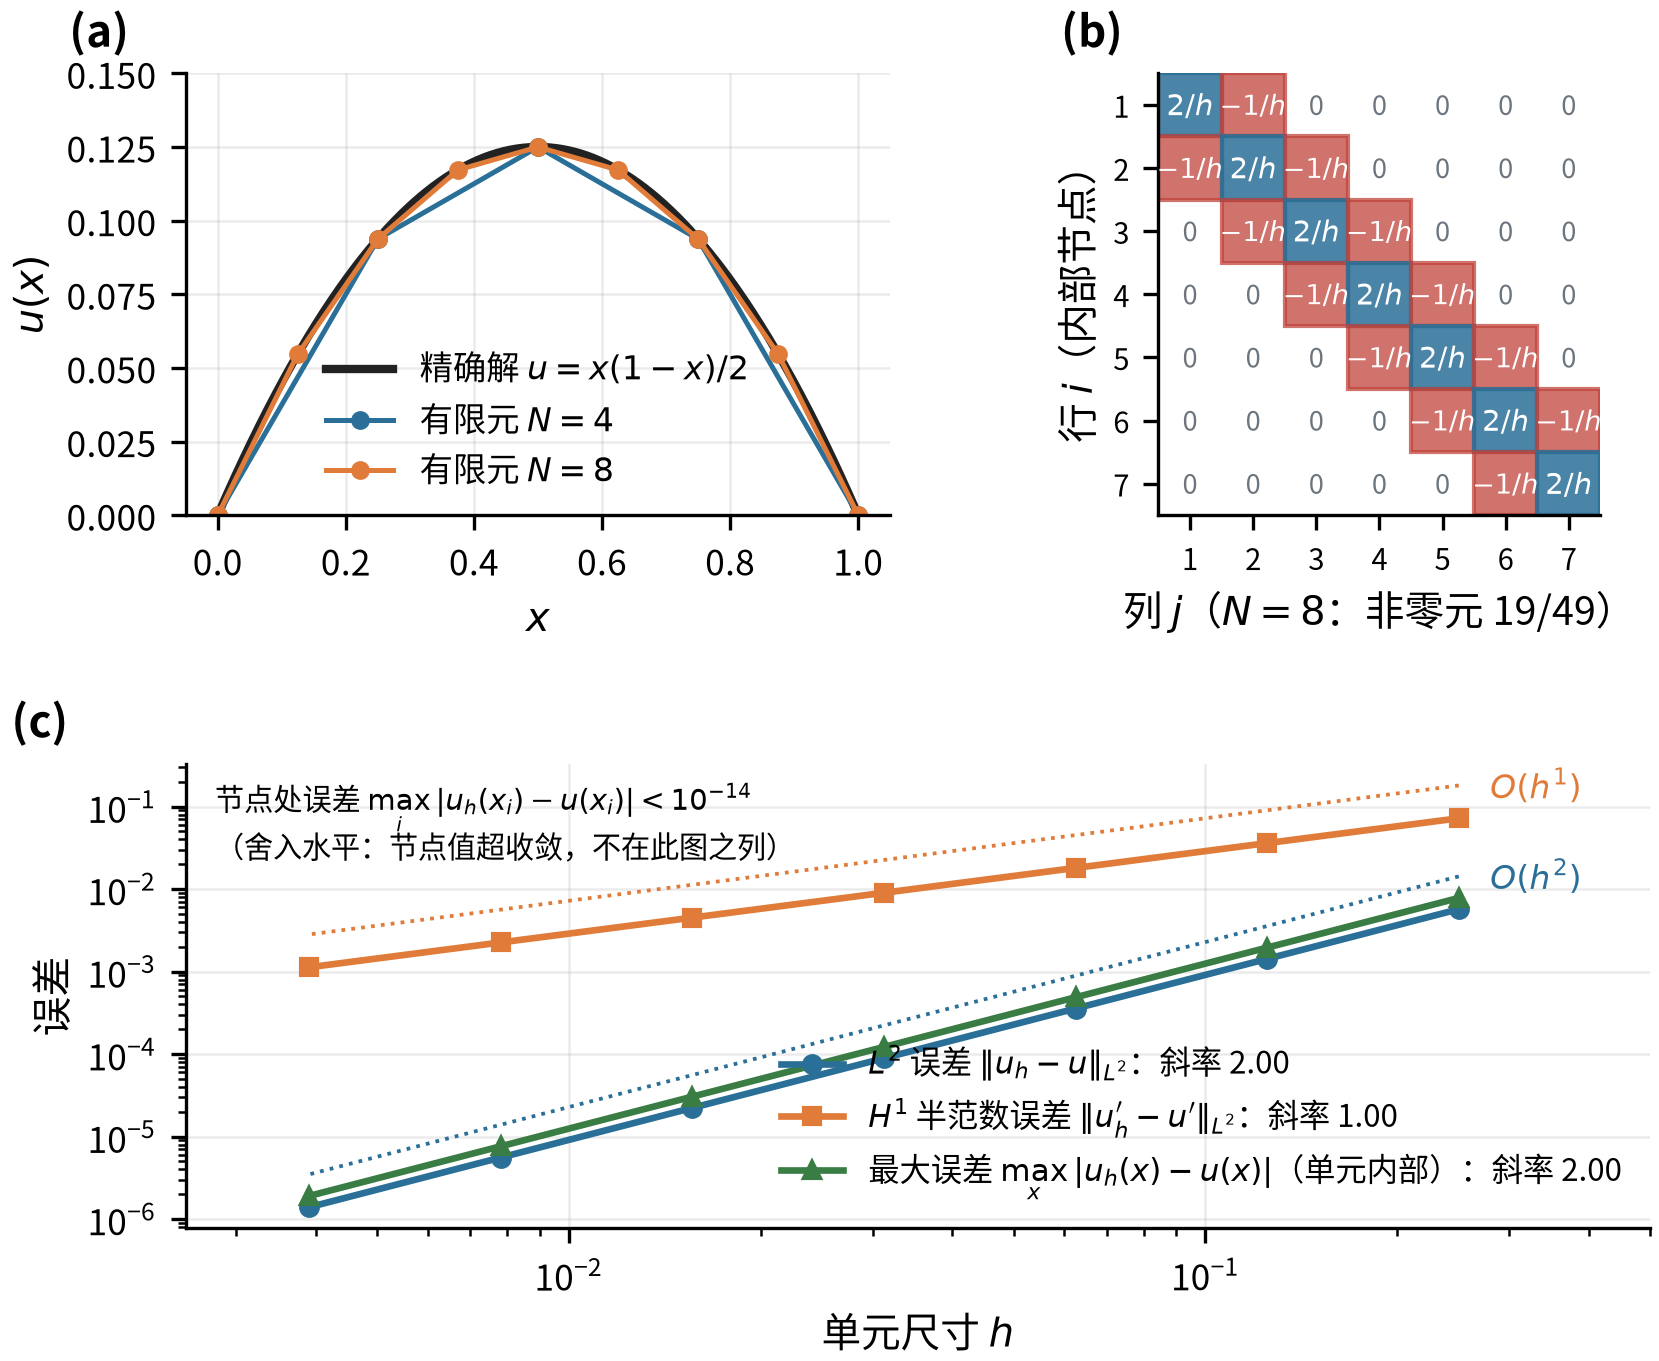
\includegraphics[width=0.95\textwidth]{figs_chap13/chap13_fig2.png}
\caption{一维有限元求解热传导问题$-u''=1$，$u(0)=u(1)=0$。(a) 有限元解（$N=4,8$）与解析解$u(x)=x(1-x)/2$的对比：节点值与解析解重合，误差只出现在单元内部。(b) 施加边界条件后的刚度矩阵$K$（$N=8$）的三对角结构——这源于帐篷函数的局部支撑性。(c) 网格细化时的收敛：$L^2$误差和单元内最大误差按$O(h^2)$下降（拟合斜率2.00），$H^1$半范数误差按$O(h)$下降（斜率1.00）；节点处的误差在$10^{-14}$以下（舍入水平），这是一维线性元的超收敛现象。}
\label{fig:chap13_fem}
\end{figure}

% ------------------------------------------------------------------------------------
\section{单元组装：从局部到整体}

上一节我们直接写出了整体刚度矩阵，这在一维均匀网格上没有问题；可一旦网格不规则、单元类型混杂，逐个推导 $K_{ij}$ 就无从下手了。实际计算中的做法分两步：先在每个小\textbf{单元}上计算\textbf{单元刚度矩阵}，再把所有单元刚度矩阵\textbf{组装}成整体刚度矩阵。这种“分而治之”的策略使有限元方法非常灵活——可以处理不规则网格、不同类型的单元混合等。

\subsection{单元刚度矩阵}

对于一维线性单元（两个节点），单元刚度矩阵是 $2 \times 2$ 的：

\begin{keyformula}[title=一维线性单元刚度矩阵]
\begin{equation}
K^e = \frac{1}{h}
\begin{pmatrix}
1 & -1 \\
-1 & 1
\end{pmatrix}
\end{equation}

行和列分别对应单元的左节点和右节点。
\end{keyformula}

\paragraph{推导}

设单元长度为 $h$，两端节点为 $x_L$ 和 $x_R$。

单元内的两个形函数：
\[
N_L(x) = \frac{x_R - x}{h}, \quad N_R(x) = \frac{x - x_L}{h}
\]

它们的导数：
\[
N_L' = -\frac{1}{h}, \quad N_R' = \frac{1}{h}
\]

单元刚度矩阵的元素：
\[
K^e_{LL} = \int_{x_L}^{x_R} (N_L')^2 dx = \frac{1}{h^2} \cdot h = \frac{1}{h}
\]
\[
K^e_{LR} = \int_{x_L}^{x_R} N_L' N_R' dx = -\frac{1}{h^2} \cdot h = -\frac{1}{h}
\]
\[
K^e_{RR} = \int_{x_L}^{x_R} (N_R')^2 dx = \frac{1}{h^2} \cdot h = \frac{1}{h}
\]

\subsection{组装过程}

组装的规则很简单：把每个单元刚度矩阵“放入”整体矩阵的对应位置，重叠处累加。

\begin{figure}[htbp]
\centering
\begin{tikzpicture}[scale=0.6]
    % 单元1矩阵（用数学矩阵表示，不用tikz框）
    \node[anchor=east] at (-2,6) {\small 单元1 (节点0-1):};
    \node at (0,6) {$\begin{pmatrix} \frac{1}{h} & -\frac{1}{h} \\[3pt] -\frac{1}{h} & \frac{1}{h} \end{pmatrix}$};

    % 箭头指向蓝色区域
    \draw[->, thick, blue!70] (1.8,6) -- (4.2,4.5);

    % 单元2矩阵
    \node[anchor=east] at (-2,2) {\small 单元2 (节点1-2):};
    \node at (0,2) {$\begin{pmatrix} \frac{1}{h} & -\frac{1}{h} \\[3pt] -\frac{1}{h} & \frac{1}{h} \end{pmatrix}$};

    % 箭头指向橙色区域
    \draw[->, thick, orange!80] (1.8,2) -- (5.2,2.5);

    % 整体矩阵框架
    \draw[thick] (4,0) grid (9,5);

    % 填充蓝色区域（单元1贡献：节点0,1）
    \fill[blue!25] (4,4) rectangle (5,5);
    \fill[blue!25] (5,4) rectangle (6,5);
    \fill[blue!25] (4,3) rectangle (5,4);
    \fill[blue!25] (5,3) rectangle (6,4);

    % 填充橙色区域（单元2贡献：节点1,2）
    \fill[orange!25] (5,3) rectangle (6,4);
    \fill[orange!25] (6,3) rectangle (7,4);
    \fill[orange!25] (5,2) rectangle (6,3);
    \fill[orange!25] (6,2) rectangle (7,3);

    % 重叠处（节点1的对角元）用红色标出
    \fill[red!40] (5,3) rectangle (6,4);
    \node[font=\footnotesize] at (5.5,3.5) {$\frac{2}{h}$};

    % 列标签（在矩阵上方）
    \foreach \i in {0,...,4} {
        \node[above, font=\scriptsize] at (4.5+\i,5.1) {\i};
    }
    % 行标签（在矩阵左侧）
    \foreach \i in {0,...,4} {
        \node[left, font=\scriptsize] at (3.9,4.5-\i) {\i};
    }

    % 整体矩阵标题
    \node[above] at (6.5,5.5) {\small 整体刚度矩阵 $K$};

    % 说明文字
    \node at (6.5,-0.8) {\small 重叠处累加：$\frac{1}{h} + \frac{1}{h} = \frac{2}{h}$};
\end{tikzpicture}
\caption{组装过程示意：单元矩阵放入整体矩阵对应位置，重叠处累加}
\end{figure}

\begin{physicalmeaning}
\textbf{组装的物理意义}：对角线元素 $K_{ii}$ 累加了所有与节点 $i$ 相连的单元贡献，是节点的“总刚度”；非对角线元素 $K_{ij}$ 只来自同时包含 $i$ 和 $j$ 的单元，是节点间的“耦合”。这就像一个弹簧网络：每个节点的总刚度是连接它的所有弹簧刚度之和。
\end{physicalmeaning}

% ------------------------------------------------------------------------------------
\section{边界条件处理}

到目前为止，边界条件是靠“只对内部节点列方程”悄悄处理掉的。这一节把这件事摆到明面上：边界条件到底怎么进入方程组，有几种进入方式，以及为什么其中一种会把第1章的乘子带回来。

\subsection{Dirichlet 边界条件（固定值）}

我们的例子中，$u(0) = u(1) = 0$ 是 Dirichlet 边界条件——边界上的值是固定的。

\paragraph{处理方法1：直接消去}

既然 $U_0 = U_4 = 0$ 是已知的，就从方程组中删去这两个未知量，只求解内部节点。

这就是我们上面手算例子用的方法。

\paragraph{处理方法2：大数法（罚函数）}

把对角线元素改成一个很大的数，对应的载荷也相应修改：

\[
K_{00} \leftarrow 10^{20}, \quad F_0 \leftarrow 10^{20} \times g_0
\]

其中 $g_0$ 是边界值。这样方程 $10^{20} U_0 = 10^{20} g_0$ 就强制 $U_0 \approx g_0$。

\textbf{优点}：不改变矩阵结构，易于编程

\textbf{缺点}：矩阵条件数变差

\subsection{Neumann 边界条件（给定导数）}

如果边界条件是 $u'(1) = q$（给定热流），这是 Neumann 边界条件。

Neumann 条件在弱形式中\textbf{自然满足}——它会贡献到载荷向量：
\[
F_n \leftarrow F_n + q
\]

\subsection{拉格朗日乘子法}

和第1章一样，我们也可以用拉格朗日乘子处理边界条件！

把边界条件 $u(0) = g$ 看作约束，引入乘子 $\lambda$：
\[
\mathcal{L}[u, \lambda] = J[u] + \lambda(u(0) - g)
\]

这导出一个\textbf{鞍点问题}：
\[
\begin{pmatrix}
K & B^\top \\
B & 0
\end{pmatrix}
\begin{pmatrix}
U \\
\lambda
\end{pmatrix}
=
\begin{pmatrix}
F \\
g
\end{pmatrix}
\]

\begin{physicalmeaning}
$\lambda$ 的物理意义是边界处的\textbf{法向通量}：在热传导里，$\lambda$ 是热流密度（W/m²）；在弹性力学里，$\lambda$ 是边界反力（N）。这与第5章力学中的约束力完全对应——边界条件本质上也是约束！
\end{physicalmeaning}
\review{第1章}{影子价格：$\lambda = -\dfrac{df^*}{d\epsilon}$。这里的 $\epsilon$ 是边界温度 $g$ 的微小改变，$f^*$ 是最小总势能。所以 $\lambda$ 度量“边界值抬高一点，总势能变多少”——量纲恰好是热流。}

% ------------------------------------------------------------------------------------
\section{误差分析与收敛性}

\subsection{误差的来源}

有限元解 $u_h$ 与精确解 $u$ 之间有误差。误差来自哪里？一方面是\textbf{离散化误差}——我们用有限维空间逼近了无限维空间；另一方面是\textbf{插值误差}——我们用分片多项式逼近了光滑函数。两者都随网格加密而减小，问题是减小得多快。

\subsection{误差估计}

对于线性形函数，误差有如下估计：

\begin{keytheorem}[title=有限元误差估计]
设 $u$ 是精确解，$u_h$ 是线性有限元解，$h$ 是网格步长。则：

\textbf{能量范数误差}：
\[
\|u' - u_h'\|_{L^2} \leq Ch \|u''\|_{L^2}
\]

\textbf{$L^2$ 范数误差}：
\[
\|u - u_h\|_{L^2} \leq Ch^2 \|u''\|_{L^2}
\]

其中 $C$ 是与 $h$ 无关的常数。
\end{keytheorem}

\paragraph{含义}

网格加密一倍（$h \to h/2$），导数误差减半，函数值误差减到 $\frac{1}{4}$。也就是说，线性元的收敛阶在能量范数下是 $O(h)$，在 $L^2$ 范数下是 $O(h^2)$；若用更高阶的多项式（如二次元、三次元），可以获得更高的收敛阶。

\subsection{数值验证}

让我们用不同的网格密度求解 $-u'' = 1$，验证收敛性：

\begin{center}
\begin{tabular}{c|c|c|c}
\toprule
单元数 $N$ & 步长 $h$ & 最大误差 & 误差比 \\
\midrule
4 & 0.25 & $7.8 \times 10^{-3}$ & -- \\
8 & 0.125 & $2.0 \times 10^{-3}$ & 3.9 \\
16 & 0.0625 & $4.9 \times 10^{-4}$ & 4.1 \\
32 & 0.03125 & $1.2 \times 10^{-4}$ & 4.1 \\
\bottomrule
\end{tabular}
\end{center}

每次加密一倍，误差减少到约 $\frac{1}{4}$——符合 $O(h^2)$ 的理论预测！
\clarify{表中的“最大误差”取在单元中点。前面说过一维线性元在节点处是精确的，所以误差全部来自节点之间的线性插值，中点误差恰好是 $h^2/8$（$h = 0.25$ 时为 $0.0078$）。}

% ------------------------------------------------------------------------------------
\section{二维问题简介}

\subsection{从一维到二维}

一维的思想可以自然推广到二维。

\textbf{二维 Poisson 方程}：
\[
-\nabla^2 u = -\left(\frac{\partial^2 u}{\partial x^2} + \frac{\partial^2 u}{\partial y^2}\right) = f \quad \text{in } \Omega
\]

\textbf{弱形式}：
\[
\int_\Omega \nabla u \cdot \nabla v \, dA = \int_\Omega fv \, dA
\]

\textbf{离散化}：把区域 $\Omega$ 剖分成三角形或四边形单元。

\begin{figure}[htbp]
\centering
\begin{tikzpicture}[scale=0.8]
    % 区域
    \draw[thick] (0,0) -- (4,0) -- (4,3) -- (0,3) -- cycle;
    
    % 三角形网格
    \foreach \x in {0,1,...,4} {
        \foreach \y in {0,1,2,3} {
            \fill (\x,\y) circle (1.5pt);
        }
    }
    
    % 画一些三角形
    \draw[gray] (0,0) -- (1,1) -- (0,1) -- cycle;
    \draw[gray] (0,0) -- (1,0) -- (1,1) -- cycle;
    \draw[gray] (1,0) -- (2,1) -- (1,1) -- cycle;
    \draw[gray] (1,0) -- (2,0) -- (2,1) -- cycle;
    \draw[gray] (2,0) -- (3,1) -- (2,1) -- cycle;
    \draw[gray] (2,0) -- (3,0) -- (3,1) -- cycle;
    \draw[gray] (3,0) -- (4,1) -- (3,1) -- cycle;
    \draw[gray] (3,0) -- (4,0) -- (4,1) -- cycle;
    
    \draw[gray] (0,1) -- (1,2) -- (0,2) -- cycle;
    \draw[gray] (0,1) -- (1,1) -- (1,2) -- cycle;
    \draw[gray] (1,1) -- (2,2) -- (1,2) -- cycle;
    \draw[gray] (1,1) -- (2,1) -- (2,2) -- cycle;
    \draw[gray] (2,1) -- (3,2) -- (2,2) -- cycle;
    \draw[gray] (2,1) -- (3,1) -- (3,2) -- cycle;
    \draw[gray] (3,1) -- (4,2) -- (3,2) -- cycle;
    \draw[gray] (3,1) -- (4,1) -- (4,2) -- cycle;
    
    \draw[gray] (0,2) -- (1,3) -- (0,3) -- cycle;
    \draw[gray] (0,2) -- (1,2) -- (1,3) -- cycle;
    \draw[gray] (1,2) -- (2,3) -- (1,3) -- cycle;
    \draw[gray] (1,2) -- (2,2) -- (2,3) -- cycle;
    \draw[gray] (2,2) -- (3,3) -- (2,3) -- cycle;
    \draw[gray] (2,2) -- (3,2) -- (3,3) -- cycle;
    \draw[gray] (3,2) -- (4,3) -- (3,3) -- cycle;
    \draw[gray] (3,2) -- (4,2) -- (4,3) -- cycle;
    
    % 标注
    \node at (2,-0.8) {三角形网格剖分};
\end{tikzpicture}
\caption{二维有限元：区域被剖分成三角形单元}
\end{figure}

\subsection{三角形单元}

最简单的二维单元是线性三角形单元。每个三角形有 3 个节点，单元内的近似解是：
\[
u_h(x, y) = U_1 N_1(x,y) + U_2 N_2(x,y) + U_3 N_3(x,y)
\]

其中 $N_i$ 是线性形函数，满足 $N_i(x_j, y_j) = \delta_{ij}$。

\paragraph{单元刚度矩阵}

三角形单元的刚度矩阵是 $3 \times 3$：
\[
K^e_{ij} = \int_{\text{三角形}} \nabla N_i \cdot \nabla N_j \, dA
\]

由于 $N_i$ 是线性函数，$\nabla N_i$ 是常向量，积分很容易计算。

\subsection{刚度矩阵的稀疏性}

二维问题的刚度矩阵仍然是稀疏的——只有相邻节点之间有耦合。

但稀疏结构更复杂：不再是三对角，而是\textbf{带状稀疏}矩阵。

\begin{figure}[htbp]
\centering
\begin{tikzpicture}[scale=0.08]
    % 画一个稀疏矩阵的样子
    \draw[gray] (0,0) rectangle (50,50);
    
    % 用随机点表示非零元素
    \foreach \i in {0,...,49} {
        \fill[blue] (\i,49-\i) circle (1);
        \pgfmathsetmacro{\jone}{int(\i+1)}
        \pgfmathsetmacro{\jtwo}{int(\i+2)}
        \pgfmathsetmacro{\jthree}{int(\i+5)}
        \pgfmathsetmacro{\jfour}{int(\i+6)}
        \ifnum\i<49
            \fill[blue!50] (\jone,49-\i) circle (0.8);
            \fill[blue!50] (\i,49-\jone) circle (0.8);
        \fi
        \ifnum\i<48
            \fill[blue!30] (\jtwo,49-\i) circle (0.6);
            \fill[blue!30] (\i,49-\jtwo) circle (0.6);
        \fi
        \ifnum\i<45
            \fill[blue!20] (\jthree,49-\i) circle (0.5);
            \fill[blue!20] (\i,49-\jthree) circle (0.5);
        \fi
    }
    
    \node at (25,-8) {\small 二维有限元的稀疏刚度矩阵};
\end{tikzpicture}
\end{figure}

% ------------------------------------------------------------------------------------
% ------------------------------------------------------------------------------------
\section{殊途同归：有限差分与有限元}

在继续深入之前，让我们回答一个常见问题：有限差分法（FDM）和有限元法（FEM）有什么区别？

\subsection{一维情况：完全等价}

考虑一维问题 $-u'' = f$，用 $N$ 个等距节点离散化。

\begin{figure}[htbp]
\centering
\begin{tikzpicture}[scale=1.2]
    % 左边：FDM
    \node[font=\bfseries] at (-3, 2) {有限差分 (FDM)};
    \draw[->] (-5, 0) -- (-1, 0) node[right] {$x$};
    \foreach \i in {0,1,2,3,4} {
        \fill (-5+\i, 0) circle (2pt);
        \node[below] at (-5+\i, -0.2) {\small $x_\i$};
    }
    % Taylor展开示意
    \draw[blue, thick, ->] (-3, 0.3) -- (-4, 0.3);
    \draw[blue, thick, ->] (-3, 0.3) -- (-2, 0.3);
    \node[blue, above] at (-3, 0.4) {\small Taylor展开};
    
    % 右边：FEM
    \node[font=\bfseries] at (3, 2) {有限元 (FEM)};
    \draw[->] (1, 0) -- (5, 0) node[right] {$x$};
    \foreach \i in {0,1,2,3,4} {
        \fill (1+\i, 0) circle (2pt);
    }
    % 形函数示意
    \draw[red, thick] (1,0) -- (2,0.8) -- (3,0);
    \draw[red, thick] (2,0) -- (3,0.8) -- (4,0);
    \node[red, above] at (3, 0.9) {\small 形函数};
\end{tikzpicture}
\caption{有限差分 vs 有限元的离散化方式}
\end{figure}

\vspace{0.3cm}
\noindent
\begin{minipage}[t]{0.48\textwidth}
\textbf{有限差分的推导}

出发点：Taylor展开近似导数
\[
-u''(x_i) \approx -\frac{u_{i+1} - 2u_i + u_{i-1}}{h^2}
\]

离散方程（第 $i$ 行）：
\[
\frac{-u_{i-1} + 2u_i - u_{i+1}}{h^2} = f_i
\]

系数：$\left[ -\frac{1}{h^2}, \; \frac{2}{h^2}, \; -\frac{1}{h^2} \right]$
\end{minipage}
\hfill
\begin{minipage}[t]{0.48\textwidth}
\textbf{有限元的推导}

出发点：弱形式 + 线性形函数
\[
K_{ij} = \int \phi_i' \phi_j' dx
\]

刚度矩阵（第 $i$ 行）：
\[
\frac{1}{h} [-1, \quad 2, \quad -1]
\]

方程：$\frac{-U_{i-1} + 2U_i - U_{i+1}}{h} = hf_i$
\end{minipage}

\vspace{0.5cm}
把FEM方程两边除以 $h$：
\[
\frac{-U_{i-1} + 2U_i - U_{i+1}}{h^2} = f_i
\]

\begin{insightbox}
在一维均匀网格上，线性有限元和中心差分给出\textbf{完全相同}的方程！

这不是巧合——两种方法从不同角度逼近了同一个物理问题。
\end{insightbox}



\subsection{二维情况：分道扬镳}

当问题升级到二维，两种方法开始展现本质区别。

\textbf{任务}：在圆形区域 $\Omega$ 上求解 $-\Delta u = f$。

\begin{figure}[htbp]
\centering
\begin{tikzpicture}[scale=1.8]
    % 左边：FDM
    \begin{scope}[xshift=-3cm]
        \node[font=\bfseries] at (0.5, 1.3) {有限差分};
        % 规则网格
        \draw[step=0.2, gray!30, thin] (0,0) grid (1.1,1.1);
        % 真实圆边界
        \draw[thick, red] (0,1) arc (90:0:1);
        % 锯齿逼近
        \draw[blue, thick]
            (0,1) -- (0.2,1) -- (0.2,0.8) --
            (0.4,0.8) -- (0.4,0.6) --
            (0.6,0.6) -- (0.6,0.4) --
            (0.8,0.4) -- (0.8,0.2) --
            (1.0,0.2) -- (1.0,0);
        % 五点差分模板
        \fill[blue] (0.6,0.4) circle (1pt);
        \foreach \dx/\dy in {0.2/0, -0.2/0, 0/0.2, 0/-0.2}{
            \draw[->, thick, blue!60] (0.6,0.4) -- +(\dx,\dy);
        }
        \node[red, font=\scriptsize] at (0.5, 1.15) {真实边界};
        \node[blue, font=\scriptsize] at (0.2, 0.5) {锯齿};
    \end{scope}
    
    % 右边：FEM
    \begin{scope}[xshift=1.5cm]
        \node[font=\bfseries] at (0.5, 1.3) {有限元};
        % 真实圆边界
        \draw[thick, red] (0,1) arc (90:0:1);
        % 三角剖分
        \coordinate (O) at (0,0);
        \coordinate (B) at (0,1);
        \coordinate (C) at (0.5,0.866);
        \coordinate (D) at (0.866,0.5);
        \coordinate (E) at (1,0);
        \coordinate (b) at (0,0.5);
        \coordinate (c) at (0.25,0.433);
        \coordinate (d) at (0.433,0.25);
        \coordinate (e) at (0.5,0);
        
        \draw[blue] (O) -- (b) -- (c) -- cycle;
        \draw[blue] (O) -- (c) -- (d) -- cycle;
        \draw[blue] (O) -- (d) -- (e) -- cycle;
        \draw[blue] (b) -- (B) -- (C) -- (c) -- cycle;
        \draw[blue] (c) -- (C) -- (D) -- (d) -- cycle;
        \draw[blue] (d) -- (D) -- (E) -- (e) -- cycle;
        
        % 边界节点
        \foreach \P in {B,C,D,E} {
            \fill[red] (\P) circle (1.5pt);
        }
        \node[blue, font=\scriptsize] at (0.5, 0.5) {三角形};
        \node[red, font=\scriptsize] at (0.7, 1.0) {节点在边界上};
    \end{scope}
\end{tikzpicture}
\caption{二维圆形区域的离散化：FDM用锯齿逼近边界，FEM可以精确贴合。}
\end{figure}

\begin{center}
\renewcommand{\arraystretch}{1.4}
\begin{tabular}{l|p{5cm}|p{5cm}}
\toprule
& \textbf{有限差分} & \textbf{有限元} \\
\midrule
网格类型 & 结构化（规则方格） & 非结构化（任意三角形） \\
边界处理 & 锯齿逼近，精度损失 & 节点直接在边界上 \\
复杂几何 & 困难（需要特殊处理） & 自然（只需网格生成） \\
实现难度 & 简单（数组索引） & 复杂（邻接关系） \\
适用场景 & 规则区域（图像、芯片） & 复杂几何（飞机、骨骼） \\
\bottomrule
\end{tabular}
\end{center}

\begin{physicalmeaning}
\textbf{为什么FEM统治了工程计算？}

现实世界的几何很少是规则的：飞机机翼是流线型的，人体骨骼是弯曲的，汽车车身是复杂曲面。

有限元的三角形/四面体网格可以\textbf{贴合任意几何形状}，这是它在工程中广泛应用的根本原因。

代价是：需要维护复杂的网格数据结构和邻接关系。
\end{physicalmeaning}

% ------------------------------------------------------------------------------------
\section{连续性的秘密}

\subsection{为什么要求连续？}

在前面的推导中，我们默默假设了 $u_h(x)$ 是连续的。但为什么？

\begin{figure}[htbp]
\centering
\begin{tikzpicture}[scale=1.2]
    % 上半部分：连续函数
    \begin{scope}[yshift=2cm]
        \draw[->] (0,0) -- (4,0) node[right] {$x$};
        \draw[->] (0,0) -- (0,1.5);
        \draw[blue, very thick] (0.5, 0.3) -- (2, 1.2) -- (3.5, 0.8);
        \node[blue] at (2, 1.5) {连续折线};
        \node[blue, align=center] at (5, 0.8) {导数有限 \\ 能量有限 $\checkmark$};
    \end{scope}
    
    % 下半部分：不连续函数
    \begin{scope}
        \draw[->] (0,0) -- (4,0) node[right] {$x$};
        \draw[->] (0,0) -- (0,1.5);
        \draw[red, very thick] (0.5, 0.3) -- (2, 1.2);
        \draw[red, very thick] (2, 0.4) -- (3.5, 0.8);
        \draw[red, dashed] (2, 0.4) -- (2, 1.2);
        \node[red] at (2.3, 0.8) {Jump!};
        \node[red, align=center] at (5, 0.8) {导数 $= \infty$ \\ 能量 $= \infty$ $\times$};
    \end{scope}
\end{tikzpicture}
\caption{连续性与能量的关系}
\end{figure}

\textbf{数学解释}：我们的弱形式包含梯度项 $\int |\nabla u|^2 dx$（能量）。如果 $u$ 在某点有跳跃（不连续），导数 $u'$ 在该点就变成 Dirac $\delta$ 函数（无穷大），于是能量 $\int (u')^2 dx = \int \delta^2 dx = \infty$。物理上，无穷大的能量是不允许的。

\begin{keyformula}[title=$C^0$ 连续性]
我们要求有限元解空间 $V_h \subset C^0(\Omega)$，即：

\textbf{函数值连续，但导数可以不连续}

换句话说：$u_h$ 可以“折”，但不能“断”。
\end{keyformula}

\subsection{线性单元如何保证连续？}

一个关键问题：我们只要求\textbf{节点值}相等，怎么能保证整条公共边上都连续？

\begin{figure}[htbp]
\centering
\begin{tikzpicture}[scale=1.5]
    % 两个三角形共享边
    \coordinate (N1) at (0,1);
    \coordinate (N2) at (0,-1);
    \coordinate (N3) at (-1.5, 0);
    \coordinate (N4) at (1.5, 0);
    
    \draw[fill=blue!10] (N1) -- (N2) -- (N3) -- cycle;
    \draw[fill=orange!10] (N1) -- (N2) -- (N4) -- cycle;
    
    % 共享边
    \draw[ultra thick, red] (N1) -- (N2);
    
    % 节点标注
    \node[above] at (N1) {$U_1$};
    \node[below] at (N2) {$U_2$};
    \node[left] at (N3) {$U_3$};
    \node[right] at (N4) {$U_4$};
    
    \node[blue] at (-0.7, 0) {单元 A};
    \node[orange] at (0.7, 0) {单元 B};
    
    % 边上的点
    \fill[black] (0, 0.3) circle (1.5pt) node[right] {$P$};
\end{tikzpicture}
\caption{两个三角形共享边 1-2}
\end{figure}

\textbf{几何证明}：

\begin{enumerate}
    \item 在三角形 A 内部，$u_h$ 是一个\textbf{平面}（线性函数）
    
    \item 这个平面在边 1-2 上截出一条\textbf{直线}
    
    \item 这条直线由两个端点值 $U_1$ 和 $U_2$ \textbf{唯一确定}（两点定一线！）
    
    \item 同样，三角形 B 在边 1-2 上也截出一条直线，也由 $U_1$ 和 $U_2$ 确定
    
    \item 两条直线端点相同 $\Rightarrow$ 两条直线重合！
\end{enumerate}

\begin{insightbox}
\textbf{线性单元连续性的关键}：两点确定一条直线。

只要共享节点的值相同，整条公共边就自动连续——就像\textbf{合页(Hinge)}一样严丝合缝。

这就是为什么线性单元只需要在顶点处设置自由度。
\end{insightbox}

\textbf{高阶单元怎么办？}

如果是二次单元，边上的函数是抛物线。两点定不了抛物线！

解决方案：在边的中点增加一个节点，三点定抛物线。

\begin{figure}[htbp]
\centering
\begin{tikzpicture}[scale=1.2]
    % 线性单元
    \begin{scope}
        \node[font=\bfseries] at (1, 1.8) {线性单元};
        \draw[thick] (0,0) -- (2,0) -- (1,1.5) -- cycle;
        \fill[blue] (0,0) circle (3pt);
        \fill[blue] (2,0) circle (3pt);
        \fill[blue] (1,1.5) circle (3pt);
        \node[below] at (1, -0.3) {3个节点};
    \end{scope}
    
    % 二次单元
    \begin{scope}[xshift=5cm]
        \node[font=\bfseries] at (1, 1.8) {二次单元};
        \draw[thick] (0,0) -- (2,0) -- (1,1.5) -- cycle;
        % 顶点
        \fill[blue] (0,0) circle (3pt);
        \fill[blue] (2,0) circle (3pt);
        \fill[blue] (1,1.5) circle (3pt);
        % 边中点
        \fill[red] (1,0) circle (3pt);
        \fill[red] (1.5,0.75) circle (3pt);
        \fill[red] (0.5,0.75) circle (3pt);
        \node[below] at (1, -0.3) {6个节点};
    \end{scope}
\end{tikzpicture}
\caption{线性单元（3节点）vs 二次单元（6节点）}
\end{figure}

\subsection{一维二次单元详解}

为了理解高阶单元，让我们先看最简单的情况：一维二次单元。

\begin{figure}[htbp]
\centering
\begin{tikzpicture}[scale=1.5]
    % 坐标轴
    \draw[->] (-0.5, 0) -- (4.5, 0) node[right] {$x$};
    \draw[->] (0, -0.3) -- (0, 1.5);
    
    % 三个节点
    \fill[blue] (0, 0) circle (3pt) node[below] {$x_1 = 0$};
    \fill[red] (2, 0) circle (3pt) node[below] {$x_2 = h/2$};
    \fill[blue] (4, 0) circle (3pt) node[below] {$x_3 = h$};
    
    % 三个形函数
    % φ_1: 在x_1=1, 其他=0
    \draw[blue, thick, domain=0:4, samples=50] plot (\x, {((\x-2)*(\x-4))/((-2)*(-4))});
    \node[blue] at (0.3, 1.2) {$\phi_1$};
    
    % φ_2: 在x_2=1, 其他=0
    \draw[red, thick, domain=0:4, samples=50] plot (\x, {((\x-0)*(\x-4))/((2-0)*(2-4))});
    \node[red] at (2, 1.3) {$\phi_2$};
    
    % φ_3: 在x_3=1, 其他=0
    \draw[green!60!black, thick, domain=0:4, samples=50] plot (\x, {((\x-0)*(\x-2))/((4-0)*(4-2))});
    \node[green!60!black] at (3.7, 1.2) {$\phi_3$};
    
    % 高度标记
    \draw[dashed, gray] (0, 1) -- (0.2, 1);
    \node[left, gray] at (0, 1) {\small 1};
    \draw[dashed, gray] (2, 1) -- (2.2, 1);
    \draw[dashed, gray] (4, 1) -- (4.2, 1);
\end{tikzpicture}
\caption{一维二次单元的三个形函数：都是抛物线！}
\end{figure}

\textbf{二次形函数的公式}

用拉格朗日插值构造（三点定抛物线）：

\begin{align}
\phi_1(x) &= \frac{(x - x_2)(x - x_3)}{(x_1 - x_2)(x_1 - x_3)} = \frac{(x - h/2)(x - h)}{(0 - h/2)(0 - h)} = \frac{2(x - h/2)(x - h)}{h^2} \\[5pt]
\phi_2(x) &= \frac{(x - x_1)(x - x_3)}{(x_2 - x_1)(x_2 - x_3)} = \frac{(x - 0)(x - h)}{(h/2)(- h/2)} = -\frac{4x(x - h)}{h^2} \\[5pt]
\phi_3(x) &= \frac{(x - x_1)(x - x_2)}{(x_3 - x_1)(x_3 - x_2)} = \frac{(x - 0)(x - h/2)}{(h)(h/2)} = \frac{2x(x - h/2)}{h^2}
\end{align}

可以验证：$\phi_i(x_j) = \delta_{ij}$（在自己的节点上等于1，其他节点上等于0）。

\begin{example}[二次单元的刚度矩阵]
计算一维二次单元的刚度矩阵 $K_{ij} = \int_0^h \phi_i'(x) \phi_j'(x) dx$。

\textbf{Step 1: 求导}

先对形函数求导（注意这次导数不再是常数了！）：
\begin{align}
\phi_1'(x) &= \frac{2(2x - 3h/2)}{h^2} = \frac{4x - 3h}{h^2} \\[3pt]
\phi_2'(x) &= \frac{-4(2x - h)}{h^2} = \frac{-8x + 4h}{h^2} \\[3pt]
\phi_3'(x) &= \frac{2(2x - h/2)}{h^2} = \frac{4x - h}{h^2}
\end{align}

\textbf{Step 2: 计算 $K_{11}$}
\begin{align}
K_{11} &= \int_0^h (\phi_1')^2 dx = \int_0^h \frac{(4x - 3h)^2}{h^4} dx \\
&= \frac{1}{h^4} \int_0^h (16x^2 - 24hx + 9h^2) dx \\
&= \frac{1}{h^4} \left[ \frac{16x^3}{3} - 12hx^2 + 9h^2 x \right]_0^h \\
&= \frac{1}{h^4} \left( \frac{16h^3}{3} - 12h^3 + 9h^3 \right) = \frac{1}{h^4} \cdot \frac{7h^3}{3} = \boxed{\frac{7}{3h}}
\end{align}

\textbf{Step 3: 计算 $K_{12}$}
\begin{align}
K_{12} &= \int_0^h \phi_1' \phi_2' dx = \int_0^h \frac{(4x - 3h)(-8x + 4h)}{h^4} dx \\
&= \frac{1}{h^4} \int_0^h (-32x^2 + 40hx - 12h^2) dx \\
&= \frac{1}{h^4} \left[ -\frac{32x^3}{3} + 20hx^2 - 12h^2 x \right]_0^h \\
&= \frac{1}{h^4} \left( -\frac{32h^3}{3} + 20h^3 - 12h^3 \right) = \frac{1}{h^4} \cdot \left(-\frac{8h^3}{3}\right) = \boxed{-\frac{8}{3h}}
\end{align}

\textbf{完整的刚度矩阵}（类似计算其他元素后）：
\begin{equation}
K^{(e)} = \frac{1}{3h} \begin{pmatrix}
7 & -8 & 1 \\
-8 & 16 & -8 \\
1 & -8 & 7
\end{pmatrix}
\end{equation}
\end{example}

\begin{physicalmeaning}
对比线性单元和二次单元的刚度矩阵：

\vspace{0.3cm}
\begin{minipage}[t]{0.45\textwidth}
\centering
\textbf{线性单元}（2节点）
\[
K^{(e)} = \frac{1}{h} \begin{pmatrix}
1 & -1 \\
-1 & 1
\end{pmatrix}
\]
只有相邻节点耦合
\end{minipage}
\hfill
\begin{minipage}[t]{0.45\textwidth}
\centering
\textbf{二次单元}（3节点）
\[
K^{(e)} = \frac{1}{3h} \begin{pmatrix}
7 & -8 & 1 \\
-8 & 16 & -8 \\
1 & -8 & 7
\end{pmatrix}
\]
三个节点都有耦合！
\end{minipage}

\vspace{0.3cm}
注意二次单元中 $K_{13} = \frac{1}{3h} \neq 0$：端点1和端点3虽然不相邻，但通过中间的抛物线“感受”到彼此！
\end{physicalmeaning}

\begin{example}[精度提升的威力]
用二次单元求解 $-u'' = 1$，$u(0) = u(1) = 0$。

只用\textbf{2个二次单元}（5个节点：$x = 0, 0.25, 0.5, 0.75, 1$）：

\begin{center}
\begin{tabular}{c|c|c|c}
\toprule
$x$ & 数值解 $U$ & 精确解 $u = \frac{x(1-x)}{2}$ & 误差 \\
\midrule
0 & 0 & 0 & 0 \\
0.25 & 0.09375 & 0.09375 & 0 \\
0.5 & 0.125 & 0.125 & 0 \\
0.75 & 0.09375 & 0.09375 & 0 \\
1 & 0 & 0 & 0 \\
\bottomrule
\end{tabular}
\end{center}

误差为\textbf{零}！因为精确解是二次多项式，而二次单元可以精确表示二次多项式。

这叫做\textbf{多项式精确性}：$p$阶单元可以精确表示$p$阶及以下的多项式。
\end{example}

\begin{insightbox}
\textbf{高阶单元的代价与收益}：代价是每个单元的节点数增加（线性 3 个 $\to$ 二次 6 个），单元刚度矩阵更大、计算量增加，形函数也更复杂、需要数值积分。收益是相同网格下精度大幅提高，收敛速度从 $O(h^2)$ 提高到 $O(h^3)$，对于光滑解常常“事半功倍”。工程中的经验法则：对于光滑问题，用少量高阶单元往往比大量低阶单元更高效！
\end{insightbox}
% ------------------------------------------------------------------------------------
\section{全局视角：帐篷函数的叠加}

\subsection{从单元思维到全局思维}

前面我们一直从“拼装单元”的角度理解有限元。现在换个视角：

与其说是“把单元拼起来”，不如说是“把全局基函数叠加起来”。

\begin{figure}[htbp]
\centering
\begin{tikzpicture}[scale=0.7, x={(1cm,0cm)}, y={(0.5cm,0.4cm)}, z={(0cm,1cm)}]
    % 中心点
    \coordinate (C) at (0,0,0);
    \coordinate (Top) at (0,0,2.5);
    
    % 周围一圈点 (六边形)
    \foreach \i in {0, 60, ..., 300} {
        \coordinate (P\i) at ({2.5*cos(\i)}, {2.5*sin(\i)}, 0);
        \draw[gray] (C) -- (P\i);
        \draw[blue, thick] (Top) -- (P\i);
    }
    % 连外圈
    \draw[gray] (P0)--(P60)--(P120)--(P180)--(P240)--(P300)--cycle;
    
    % 填充几个面
    \fill[blue!20, opacity=0.5] (P0)--(Top)--(P60)--cycle;
    \fill[blue!30, opacity=0.5] (P60)--(Top)--(P120)--cycle;
    \fill[blue!15, opacity=0.5] (P120)--(Top)--(P180)--cycle;
    
    \node[above, red, font=\bfseries] at (Top) {$\Phi_i = 1$};
    \node[below] at (C) {节点 $i$};
    \node[gray] at (3, 0, 0) {$\Phi_i = 0$};
\end{tikzpicture}
\caption{全局形函数 $\Phi_i$：一个以节点 $i$ 为顶点的“帐篷”}
\end{figure}

全局形函数 $\Phi_i$ 在节点 $i$ 处取值为 1，在所有邻居节点处取值为 0，在其他地方也是 0（局部支撑），形状像一个多面体的“帐篷”或“金字塔”。有限元解可以写成：
\begin{equation}
u_h(x) = \sum_{i=1}^{N} U_i \Phi_i(x)
\end{equation}

这就是 $N$ 个帐篷高低错落地叠加在一起！

\begin{physicalmeaning}
\textbf{连续性的本质}：

每个全局基函数 $\Phi_i$ 本身都是连续的（帐篷布没有破洞）。

连续函数的线性组合还是连续函数。

所以 $u_h = \sum U_i \Phi_i$ 必然是连续的！

“节点共享”的本质，是我们定义了\textbf{跨越多个单元的全局基函数}。
\end{physicalmeaning}

\subsection{稀疏性的来源}

刚度矩阵为什么是稀疏的？

\begin{equation}
K_{ij} = \int_\Omega \nabla\Phi_i \cdot \nabla\Phi_j \, dx
\end{equation}

关键观察：$\Phi_i$ 和 $\Phi_j$ 只在它们的支撑区域重叠时，积分才非零！

\begin{figure}[htbp]
\centering
\begin{tikzpicture}[scale=1.5]
    % 中心点 i
    \coordinate (Ni) at (0,0);
    
    % i 的影响范围
    \fill[red!15] (1,0) -- (0.5, 0.866) -- (-0.5, 0.866) -- (-1,0) -- (-0.5, -0.866) -- (0.5, -0.866) -- cycle;
    
    % 画中心点
    \fill[red] (Ni) circle (2.5pt);
    \node[red, below=3pt] at (Ni) {$U_i$};
    
    % 邻居节点
    \foreach \angle/\idx in {0/1, 60/2, 120/3, 180/4, 240/5, 300/6} {
        \coordinate (Nj\idx) at (\angle:1);
        \draw[thick, gray] (Ni) -- (Nj\idx);
        \fill[blue] (Nj\idx) circle (2pt);
    }
    
    % 远处的点
    \coordinate (Nk) at (1.8, 0.8);
    \fill[black!50] (Nk) circle (2pt);
    \node[right, font=\small] at (Nk) {$U_k$（非邻居）};
    
    \draw[dashed, gray] (Ni) -- (Nk);
    \node[font=\scriptsize, gray] at (1.2, 0.5) {$K_{ik} = 0$};
\end{tikzpicture}
\caption{节点 $i$ 只与直接相邻的节点耦合}
\end{figure}

如果节点 $i$ 和 $j$ 直接相邻（有边相连），$\Phi_i$ 和 $\Phi_j$ 重叠，$K_{ij} \neq 0$；如果节点 $i$ 和 $j$ 不相邻，$\Phi_i$ 和 $\Phi_j$ 不重叠，$K_{ij} = 0$。

\begin{insightbox}
\textbf{稀疏性的物理意义}：

即使网格有100万个节点，每个节点也只与周围约6-8个邻居耦合。

刚度矩阵的每一行只有约7个非零元素（自己 + 6个邻居）。

这就是为什么我们能求解大规模有限元问题——矩阵虽大，但几乎全是零！
\end{insightbox}

% ------------------------------------------------------------------------------------
\section{与优化的联系}

让我们从拉格朗日乘子的角度重新审视有限元。

\subsection{有限元 = 能量最小化}

回顾一下有限元的推导路径：

\begin{center}
\begin{tikzpicture}[node distance=3.25cm, auto,
    block/.style={rectangle, draw, fill=blue!10, text width=2.5cm, text centered, rounded corners, minimum height=1.2cm, font=\small}]
    \node[block] (pde) {PDE\\[2pt]$-\Delta u = f$};
    \node[block, right of=pde] (var) {变分问题\\[2pt]$\min J[u]$};
    \node[block, right of=var] (weak) {弱形式\\[2pt]$\int \nabla u \cdot \nabla v = \int fv$};
    \node[block, right of=weak] (lin) {线性方程\\[2pt]$KU = F$};

    \draw[->, thick] (pde) -- (var);
    \draw[->, thick] (var) -- (weak);
    \draw[->, thick] (weak) -- (lin);
\end{tikzpicture}
\end{center}

有限元方程 $KU = F$ 其实是以下优化问题的\textbf{一阶最优性条件}：

\begin{equation}
\min_U \quad J(U) = \frac{1}{2}U^\top K U - F^\top U
\end{equation}

求导：$\nabla_U J = KU - F = 0 \quad \Rightarrow \quad KU = F$

\begin{physicalmeaning}
$J(U) = \frac{1}{2}U^\top KU - F^\top U$ 的物理意义：$\frac{1}{2}U^\top KU$ 是系统的内部能量（弹性势能、热能等），$F^\top U$ 是外力做的功，两者之差 $J(U)$ 就是总势能。\textbf{有限元求解的本质}是找到使总势能最小的状态，这与自然界的规律一致——系统总是趋向于能量最低的平衡态！
\end{physicalmeaning}

\subsection{约束处理的统一视角}

现在，边界条件可以被理解为\textbf{约束}：

\begin{center}
\renewcommand{\arraystretch}{1.5}
\begin{tabular}{c|c|c}
\toprule
\textbf{优化概念} & \textbf{有限元对应} & \textbf{物理意义} \\
\midrule
决策变量 $U$ & 节点值 $U_i$ & 温度/位移 \\
目标函数 $J(U)$ & $\frac{1}{2}U^\top KU - F^\top U$ & 总势能 \\
等式约束 $CU = g$ & Dirichlet 边界条件 & 固定边界 \\
拉格朗日乘子 $\lambda$ & 边界反力/热流 & 约束力 \\
\bottomrule
\end{tabular}
\end{center}

带边界条件的有限元问题：
\begin{align}
\min_U \quad & \frac{1}{2}U^\top K U - F^\top U \\
\text{s.t.} \quad & U_i = g_i \quad \text{（边界节点）}
\end{align}

拉格朗日函数：
\begin{equation}
\mathcal{L}(U, \lambda) = \frac{1}{2}U^\top K U - F^\top U + \sum_{i \in \text{边界}} \lambda_i (U_i - g_i)
\end{equation}

\begin{keytheorem}[title=乘子的物理意义]
有限元中的拉格朗日乘子 $\lambda_i$ = 边界节点 $i$ 处的\textbf{反力}（或热流）。

它告诉我们：\textbf{为了维持边界条件，需要施加多大的外力}。
\end{keytheorem}

\begin{example}[悬臂梁]
考虑一端固定的悬臂梁，固定端位移为零：$U_1 = 0$。

拉格朗日乘子 $\lambda_1$ 就是固定端的支反力——墙壁对梁的作用力。

如果放松约束（允许 $U_1$ 有微小位移 $\delta U_1$），最小总势能会改变 $-\lambda_1\, \delta U_1$——这正是第1章的约定 $dJ^*/dg = -\lambda$：乘子就是影子价格。
\end{example}
\review{第5章}{在第5章，乘子 $\lambda$ 给出约束力（绳子的张力、斜面的支持力）。这里的 $\lambda_1$ 是墙对梁的支反力——同一个东西，只是从“连续体”换成了“离散节点”。}

% ------------------------------------------------------------------------------------
\section{打破传统：间断有限元初探}

前面我们花了很大功夫保证有限元解的连续性。但有没有可能\textbf{故意让它不连续}？

\subsection{一个大胆的想法}

传统有限元的“痛点”都来自节点共享：必须维护复杂的节点共享关系，网格生成困难（要保证相邻单元节点对齐），也难以并行化（单元之间有耦合）。\textbf{新思路}是让每个单元拥有\textbf{独立的节点}，然后用\textbf{约束}把它们“缝合”起来！

\begin{figure}[htbp]
\centering
\begin{tikzpicture}[scale=1.5]
    % 左边：传统FEM
    \begin{scope}
        \node[font=\bfseries] at (0.75, 1.5) {传统 FEM};
        \coordinate (A) at (0,0);
        \coordinate (B) at (1.5,0);
        \coordinate (C) at (0.75, 1.2);
        \coordinate (D) at (2.25, 1.2);
        
        \draw[thick, fill=blue!10] (A)--(B)--(C)--cycle;
        \draw[thick, fill=orange!10] (B)--(D)--(C)--cycle;
        
        \fill[red] (B) circle (2pt) node[below]{$U_2$};
        \fill[red] (C) circle (2pt) node[above]{$U_3$};
        
        \node[align=center, font=\scriptsize] at (0.75, -0.5) {共享节点\\$U_2, U_3$ 只有一份};
    \end{scope}
    
    % 右边：间断FEM
    \begin{scope}[xshift=4cm]
        \node[font=\bfseries] at (0.75, 1.5) {间断 FEM};
        % 左单元
        \coordinate (A) at (0,0);
        \coordinate (B1) at (1.4,0);
        \coordinate (C1) at (0.65, 1.2);
        \draw[thick, fill=blue!10] (A)--(B1)--(C1)--cycle;
        
        % 右单元（稍微拉开）
        \coordinate (B2) at (1.6,0);
        \coordinate (C2) at (0.85, 1.2);
        \coordinate (D) at (2.35, 1.2);
        \draw[thick, fill=orange!10] (B2)--(D)--(C2)--cycle;
        
        \fill[blue] (B1) circle (2pt) node[below left=-2pt, font=\scriptsize]{$U_2^{(1)}$};
        \fill[blue] (C1) circle (2pt) node[above left=-2pt, font=\scriptsize]{$U_3^{(1)}$};
        \fill[orange] (B2) circle (2pt) node[below right=-2pt, font=\scriptsize]{$U_2^{(2)}$};
        \fill[orange] (C2) circle (2pt) node[above right=-2pt, font=\scriptsize]{$U_3^{(2)}$};
        
        \draw[<->, dashed, red] (B1)--(B2);
        \node[red, font=\scriptsize] at (1.5, -0.3) {Gap};
        
        \node[align=center, font=\scriptsize] at (0.75, -0.5) {独立节点\\需要约束缝合};
    \end{scope}
\end{tikzpicture}
\caption{传统FEM（共享节点）vs 间断FEM（独立节点）}
\end{figure}

\subsection{变量倍增与约束方程}

\textbf{变量变化}：传统做法的未知量是 $U = [U_1, U_2, U_3, U_4]$，共 4 个；间断做法把共享节点拆开，未知量变成 $U = [U_1^{(1)}, U_2^{(1)}, U_3^{(1)}, U_2^{(2)}, U_3^{(2)}, U_4^{(2)}]$，共 6 个。

\textbf{新增约束}（缝合条件）：
\begin{equation}
U_2^{(1)} = U_2^{(2)}, \quad U_3^{(1)} = U_3^{(2)}
\end{equation}

写成矩阵形式：$CU = 0$，其中
\begin{equation}
C = \begin{bmatrix}
0 & 1 & 0 & -1 & 0 & 0 \\
0 & 0 & 1 & 0 & -1 & 0
\end{bmatrix}
\end{equation}

\subsection{用拉格朗日乘子缝合}

新的优化问题：
\begin{align}
\min_U \quad & \frac{1}{2}U^\top K_{block} U - F^\top U \\
\text{s.t.} \quad & CU = 0 \quad \text{（缝合条件）}
\end{align}

其中 $K_{block}$ 是\textbf{块对角矩阵}：
\begin{equation}
K_{block} = \begin{bmatrix}
K^{(1)} & 0 \\
0 & K^{(2)}
\end{bmatrix}
\end{equation}

拉格朗日函数：
\begin{equation}
\mathcal{L}(U, \lambda) = \frac{1}{2}U^\top K_{block} U - F^\top U + \lambda^\top (CU)
\end{equation}

\begin{physicalmeaning}
乘子 $\lambda$ 的物理意义：\textbf{界面力}（interface flux）。

它是维持单元之间连续性的“胶水力”——强制两边位移相等的约束力。

这与传统FEM中隐式存在的单元间作用力是一样的，只不过现在被显式地表示出来了！
\end{physicalmeaning}

\subsection{块对角结构的威力}

间断有限元的最大优势：$K_{block}$ 是块对角的！

\begin{equation}
K_{block}^{-1} = \begin{bmatrix}
(K^{(1)})^{-1} & 0 \\
0 & (K^{(2)})^{-1}
\end{bmatrix}
\end{equation}

\textbf{这意味着}：每个单元可以\textbf{独立求解}！
\clarify{“每个单元独立求解”有个前提：界面力 $\lambda$ 已知。$\lambda$ 本身要靠界面方程解出——这正是本章扩展阅读里 Schur 补与区域分解的思路。}

\begin{center}
\renewcommand{\arraystretch}{1.4}
\begin{tabular}{l|c|c}
\toprule
& \textbf{传统 FEM} & \textbf{间断 FEM} \\
\midrule
刚度矩阵结构 & 稀疏但耦合 & 块对角 \\
单元独立求解 & 不可能 & 可以！ \\
并行化 & 困难 & 天然并行 \\
GPU 加速 & 有限 & 极度友好 \\
\bottomrule
\end{tabular}
\end{center}

\begin{insightbox}
\textbf{为什么这很重要？}

现代 GPU 有数千个核心，但它们最擅长的是做\textbf{相同的独立计算}。

间断有限元把一个大问题分解成了百万个 $3 \times 3$（或 $4 \times 4$）的小问题，每个核心解一个——这正是 GPU 的最爱！

这就是为什么间断 Galerkin (DG) 方法在计算流体力学等领域越来越流行。
\end{insightbox}

\subsection{罚函数方法：软约束}

直接处理带约束的鞍点问题比较复杂。一个常用技巧是\textbf{罚函数}：

不强制 $U^{(1)} = U^{(2)}$，而是惩罚它们的差距：
\begin{equation}
J_\rho(U) = \frac{1}{2}U^\top K_{block} U - F^\top U + \frac{\rho}{2}\|CU\|^2
\end{equation}

其中 $\rho$ 是罚参数（很大的正数）——记号与第1章“视角三：罚函数”一致。

\begin{figure}[htbp]
\centering
\begin{tikzpicture}[scale=0.9]
    % 弱罚
    \begin{scope}
        \node[font=\bfseries] at (1.5, 1.8) {弱罚（$\rho$ 小）};
        \draw[fill=blue!20, thick] (0,0) rectangle (2,1);
        \draw[fill=blue!20, thick] (2.5,0) rectangle (4.5,1);
        \draw[decorate, decoration={coil,aspect=0.5,segment length=3mm,amplitude=3mm}, thick, red] (2,0.5) -- (2.5,0.5);
        \node[red, font=\small] at (2.25, 1.3) {Gap 大};
        \node at (1, 0.5) {单元1};
        \node at (3.5, 0.5) {单元2};
    \end{scope}
    
    % 强罚
    \begin{scope}[xshift=6cm]
        \node[font=\bfseries] at (1.5, 1.8) {强罚（$\rho \to \infty$）};
        \draw[fill=blue!20, thick] (0,0) rectangle (2.1,1);
        \draw[fill=blue!20, thick] (2.2,0) rectangle (4.3,1);
        \draw[decorate, decoration={coil,aspect=0.3,segment length=1mm,amplitude=2mm}, thick, red] (2.1,0.5) -- (2.2,0.5);
        \node[red, font=\small] at (2.15, 1.3) {Gap $\approx 0$};
        \node at (1, 0.5) {单元1};
        \node at (3.25, 0.5) {单元2};
    \end{scope}
\end{tikzpicture}
\caption{罚函数就像在断口处装了一个弹簧}
\end{figure}

当 $\rho \to \infty$ 时，任何微小的 Gap 都会产生巨大的惩罚，系统被迫让 $CU \to 0$，于是恢复到传统有限元的连续解。

\begin{physicalmeaning}
罚函数的物理图像：在断口处装一个\textbf{刚度为 $\rho$ 的弹簧}。$\rho$ 小，弹簧软，拉不住，Gap 大；$\rho$ 大，弹簧硬，瞬间把两端吸在一起。这与深度学习中的正则化项异曲同工！
\[
\text{Loss} = \text{Data\_Fidelity} + \rho \cdot \text{Regularization}
\]

这个思想也激励了我们探索物理信息神经网络(PINN)。
\end{physicalmeaning}

% ------------------------------------------------------------------------------------
% ------------------------------------------------------------------------------------
\section{本章小结}

\begin{enumerate}
    \item \textbf{核心思想}：有限元方法把无限维的变分问题转化为有限维的线性方程组 $KU = F$。
    
    \item \textbf{与有限差分的关系}：一维等价，二维开始分化；FEM 的优势在于处理复杂几何。
    
    \item \textbf{连续性}：$C^0$ 连续性保证能量有限；线性单元靠“两点定一线”自动满足连续性。
    
    \item \textbf{全局视角}：有限元解是全局“帐篷”基函数的线性叠加。
    
    \item \textbf{稀疏性}：基函数的局部支撑性导致刚度矩阵稀疏。
    
    \item \textbf{优化视角}：有限元 $\Leftrightarrow$ 能量最小化 $\Leftrightarrow$ 带约束的 QP 问题。
    
    \item \textbf{间断有限元}：放弃强制连续性，用约束/罚函数缝合，获得天然并行性。
\end{enumerate}

\begin{unification}[title=有限元：优化视角的大统一]
\begin{center}
\begin{tabular}{lll}
\toprule
\textbf{优化概念} & \textbf{有限元对应} & \textbf{物理意义} \\
\midrule
决策变量 & 节点值 $U_i$ & 物理量（温度/位移） \\
目标函数 & $\frac{1}{2}U^\top KU - F^\top U$ & 总势能 \\
等式约束 & Dirichlet 边界条件 & 固定边界 \\
拉格朗日乘子 & 边界反力 & 约束力 \\
罚函数 & 界面耦合项 & 虚拟弹簧 \\
\bottomrule
\end{tabular}
\end{center}

有限元不是孤立的数值技术，它是\textbf{变分原理}和\textbf{约束优化}在工程中的自然统一！

从第1章的拉格朗日乘子，到这里的有限元，$\lambda$ 始终扮演着“约束力”的角色。
\end{unification}

\begin{physicalmeaning}
\textbf{$\lambda$ 在本章的意义}：边界条件是约束，$\lambda$ 是“把边界钉住”所需的力——热传导里是边界热流，弹性力学里是支反力，间断元里是单元之间的界面力。它仍然是影子价格：$\lambda_i = -\partial J^*/\partial g_i$，边界值放松一点，最小总势能就改变 $\lambda_i$ 那么多。

回头看：第1章的 $\lambda$ 是影子价格，第5章的 $\lambda$ 是约束力，本章把两者接在了一起——约束力就是能量对约束的敏感度。往前看：第6章机器人的接触力，以及第14章 PINN 把 PDE 当作软约束写进损失函数，用的都是同一个 $\lambda$。
\end{physicalmeaning}


% ------------------------------------------------------------------------------------
\section{习题}

\paragraph{计算题}
\begin{enumerate}
    \item 用 2 个线性单元求解 $-u'' = 1$，$u(0) = u(1) = 0$。
    \begin{enumerate}
        \item 写出刚度矩阵 $K$ 和载荷向量 $F$
        \item 求解线性方程组，得到节点值 $U_1$
        \item 与精确解 $u(0.5) = 0.125$ 比较
    \end{enumerate}
    
    \item 用 4 个线性单元求解 $-u'' = \sin(\pi x)$，$u(0) = u(1) = 0$。
    \begin{enumerate}
        \item 计算载荷向量（需要积分 $\int \sin(\pi x) \phi_i dx$）
        \item 求解节点值
        \item 与精确解 $u(x) = \frac{\sin(\pi x)}{\pi^2}$ 比较
    \end{enumerate}
    
    \item 考虑非齐次边界条件：$-u'' = 0$，$u(0) = 0$，$u(1) = 1$。
    \begin{enumerate}
        \item 用 3 个单元建立有限元方程
        \item 用直接消去法处理边界条件
        \item 求解并验证结果是直线 $u(x) = x$
    \end{enumerate}
\end{enumerate}

\paragraph{证明题}
\begin{enumerate}
    \setcounter{enumi}{3}
    \item 证明刚度矩阵 $K$ 是对称的：$K_{ij} = K_{ji}$。
    
    \item 证明刚度矩阵 $K$ 是半正定的：$U^\top K U \geq 0$ 对所有 $U$ 成立。
    
    \item 证明有限元解 $u_h$ 是精确解 $u$ 在有限元空间中的“最佳逼近”：
    \[
    \int_0^1 (u_h' - u')^2 dx \leq \int_0^1 (v_h' - u')^2 dx \quad \forall v_h \in V_h
    \]
    （提示：这叫做 Galerkin 正交性）
\end{enumerate}

\paragraph{编程题}
\begin{enumerate}
    \setcounter{enumi}{6}
    \item 实现一维线性有限元：
    \begin{enumerate}
        \item 输入：区间 $[0, 1]$，单元数 $N$，源项 $f(x)$，边界值
        \item 输出：节点值向量 $U$
        \item 测试：$-u'' = 1$，$u(0) = u(1) = 0$
    \end{enumerate}
    
    \item 做收敛性实验：
    \begin{enumerate}
        \item 用 $N = 4, 8, 16, 32, 64$ 个单元求解
        \item 计算误差 $\|u - u_h\|_{L^2}$（用数值积分）
        \item 画 $\log(\text{误差})$ vs $\log(h)$ 的图，验证 $O(h^2)$ 收敛
    \end{enumerate}
    
    \item （挑战）实现二维三角形有限元：
    \begin{enumerate}
        \item 对单位正方形用三角形网格剖分
        \item 组装刚度矩阵和载荷向量
        \item 求解 $-\nabla^2 u = 1$，$u|_{\partial\Omega} = 0$
        \item 可视化数值解
    \end{enumerate}
\end{enumerate}

\paragraph{思考题}
\begin{enumerate}
    \setcounter{enumi}{9}
    \item 有限元方法和有限差分方法有什么本质区别？各有什么优缺点？
    
    \item 为什么有限元在工程中如此成功？它解决了工程师的什么痛点？
    
    \item 有限元方法与第14章的 PINN（物理信息神经网络）有什么联系和区别？
    
    \item 如果你要模拟一架飞机的应力分布，需要多少个有限元节点？这对计算机的要求是什么？
\end{enumerate}



% ====================================================================================
% 本章原有三篇工程类扩展阅读（大规模线性方程组的求解艺术、CPU 并行计算、流固耦合有限元）
% 已移至附录D“工程专题”。
% ====================================================================================
\paragraph{延伸阅读}
想知道 $KU=F$ 在百万自由度时怎么解（共轭梯度、多重网格、条件数）、CPU 并行到底并行了什么、以及一个真实的流固耦合基准算例，请看附录D“工程专题”的前三节——它们都是本章内容的工程延伸，不影响主线阅读。
  % 第13章：PINN
% ====================================================================================
\chapter{神经算子：从函数到函数的映射}
% ====================================================================================

% ====================================================================================
\section*{引言：一次训练，任意条件}
% ====================================================================================

\sidenoteplain{神经算子的两个里程碑工作几乎同时出现：Lu Lu等人在2019年提出DeepONet，Zongyi Li等人在2020年提出FNO。两种方法代表了不同的设计哲学——DeepONet基于万能逼近定理，FNO利用傅里叶变换的效率。}

\storynote{Lu Lu}{Karniadakis 的学生，DeepONet 第一作者，也是开源库 DeepXDE 的作者——PINN 与神经算子研究的事实标准工具。DeepONet 的理论基础是 Tianping Chen 与 Hong Chen 1995 年的算子万能逼近定理，一个被埋没了二十多年的结果。}

在上一章中，我们学习了PINN：用神经网络逼近一个特定PDE的解。但你可能已经意识到一个问题：

\begin{quote}
\textit{每次初始条件或边界条件变化，我们都要重新训练网络。这太低效了！}
\end{quote}

想象一下天气预报的场景：大气动力学方程是固定的（Navier-Stokes方程），但每天的初始状态都不同。如果用PINN，每天凌晨都要花几个小时重新训练网络——这显然不切实际。

有没有办法\textbf{一次训练，对任意初始条件都能直接预测}？

这就是\textbf{神经算子}（Neural Operator）的目标：不是学习一个特定的解函数$u(x)$，而是学习从"条件函数"到"解函数"的\textbf{映射}。

\vspace{0.3cm}
\noindent\textit{为什么天气预报模型可以"一次训练、天天用"，而 PINN 却要天天重训？为什么一个在 64 个格点上训练的网络，可以直接在 256 个格点上推理？第6章辛辛苦苦组装的刚度矩阵 $K$，和这里学出来的"算子"是什么关系？}

\begin{quote}
\textbf{本章目标}：让你看到神经算子不是又一个新架构，而是第6章那句"解方程就是算 $K^{-1}F$"的直接延伸：第6章我们辛辛苦苦组装 $K$ 再去解，本章干脆从数据里把 $K^{-1}$——也就是格林函数——学出来。读完本章你会明白，为什么"一次训练、任意条件"是可能的，为什么它与网格分辨率无关，以及当我们把约束（物理定律）从损失函数里拿掉时，究竟丢掉了什么。
\end{quote}

\begin{tcolorbox}[colback=green!5, colframe=green!60!black, title=学完这章，你将能够...]
\begin{itemize}
    \item 解释为什么神经算子比PINN更适合实时预测
    \item 实现一个简化版DeepONet学习一个简单算子（反导数算子；热传导方程见习题）
    \item 理解FNO如何用傅里叶变换实现高效的全局卷积
    \item 分析神经算子与格林函数的数学联系
    \item 评估神经算子在给定任务上的适用性
\end{itemize}
\end{tcolorbox}

% ====================================================================================
\section{从求解到映射：算子学习的思想}
% ====================================================================================

\subsection{PINN的局限性}

回顾PINN的工作方式：

\begin{center}
\begin{tikzpicture}[
    box/.style={rectangle, draw, minimum width=2.5cm, minimum height=1cm, align=center},
    arrow/.style={-{Stealth}, thick}
]
    \node[box] (input) at (0, 0) {初始条件\\$u_0(x)$};
    \node[box] (pinn) at (4, 0) {PINN\\训练};
    \node[box] (output) at (8, 0) {解\\$u(x,t)$};
    
    \draw[arrow] (input) -- (pinn);
    \draw[arrow] (pinn) -- (output);
    
    \node[below=0.5cm of pinn, text=red] {每次新条件都要重训！};
\end{tikzpicture}
\end{center}

具体地，考虑热传导方程：
\begin{equation}
    \frac{\partial u}{\partial t} = \alpha \frac{\partial^2 u}{\partial x^2}, \quad u(x, 0) = u_0(x)
\end{equation}

如果$u_0(x) = \sin(\pi x)$，我们训练一个PINN得到解$u_1(x,t)$。

现在换一个初始条件$u_0(x) = \sin(2\pi x)$，我们必须\textbf{从头训练}另一个PINN得到$u_2(x,t)$。

\begin{example}[PINN的计算成本]
假设：
\begin{itemize}
    \item 训练一个PINN需要10分钟
    \item 我们需要预测1000个不同初始条件下的解
\end{itemize}
那么总计算时间是$10 \times 1000 = 10000$分钟 $\approx$ 7天！

这对于需要实时预测的应用（如天气预报）是完全不可接受的。
\end{example}

\subsection{算子学习的目标}

算子学习的思路是：既然方程是固定的，不同的只是初始/边界条件，那么我们应该学习的是\textbf{从条件到解的映射}。

\begin{definition}[解算子]
考虑PDE：
\begin{equation}
    \mathcal{L}[u] = f, \quad u|_{\partial\Omega} = g, \quad u|_{t=0} = u_0
\end{equation}
\textbf{解算子}$\mathcal{G}$是从初始/边界条件到解的映射：
\begin{equation}
    \mathcal{G}: u_0 \mapsto u
\end{equation}
其中$u_0$是输入函数，$u$是输出函数。
\end{definition}
\review{第6章}{有限元把 $-\nabla^2 u = f$ 变成 $KU = F$，解是 $U = K^{-1}F$。$K$ 只依赖方程和网格，不依赖载荷：换一个 $F$ 只需再乘一次 $K^{-1}$。"解算子"就是 $K^{-1}$ 的连续版本——本章要学的正是它。}

\begin{center}
\begin{tikzpicture}[
    box/.style={rectangle, draw, minimum width=2.5cm, minimum height=1cm, align=center},
    arrow/.style={-{Stealth}, thick}
]
    \node[box] (input1) at (0, 1) {$u_0^{(1)}(x)$};
    \node[box] (input2) at (0, 0) {$u_0^{(2)}(x)$};
    \node[box] (input3) at (0, -1) {$u_0^{(3)}(x)$};
    
    \node[box, minimum height=3cm] (operator) at (4, 0) {神经算子\\$\mathcal{G}_\theta$\\（一次训练）};
    
    \node[box] (output1) at (8, 1) {$u^{(1)}(x,t)$};
    \node[box] (output2) at (8, 0) {$u^{(2)}(x,t)$};
    \node[box] (output3) at (8, -1) {$u^{(3)}(x,t)$};
    
    \draw[arrow] (input1) -- (operator);
    \draw[arrow] (input2) -- (operator);
    \draw[arrow] (input3) -- (operator);
    \draw[arrow] (operator) -- (output1);
    \draw[arrow] (operator) -- (output2);
    \draw[arrow] (operator) -- (output3);
    
    \node[below=0.5cm of operator, text=blue] {训练后，任意新条件直接推理！};
\end{tikzpicture}
\end{center}

\begin{insightbox}
\textbf{传统神经网络} vs \textbf{神经算子}：

\begin{center}
\begin{tabular}{l|cc}
\toprule
& \textbf{传统神经网络} & \textbf{神经算子} \\
\midrule
输入 & 向量 $x \in \mathbb{R}^n$ & 函数 $u(x)$ \\
输出 & 向量 $y \in \mathbb{R}^m$ & 函数 $v(x)$ \\
学习目标 & $f: \mathbb{R}^n \to \mathbb{R}^m$ & $\mathcal{G}: \mathcal{U} \to \mathcal{V}$ \\
\bottomrule
\end{tabular}
\end{center}

神经算子是\textbf{函数空间到函数空间}的映射！
\end{insightbox}

\subsection{为什么这很难？}

函数是无穷维对象，如何用有限参数的神经网络来表示"函数到函数"的映射？

传统方法是离散化：把函数$u(x)$在网格点$\{x_1, \ldots, x_n\}$上采样，得到向量$(u(x_1), \ldots, u(x_n))$，然后用传统神经网络处理。

但这有几个问题：
\begin{enumerate}
    \item \textbf{分辨率绑定}：在$32 \times 32$网格上训练的网络，不能直接用于$64 \times 64$的输入
    \item \textbf{缺乏泛化性}：网络学到的是"像素到像素"的映射，而不是"函数到函数"的映射
    \item \textbf{网格依赖}：换一种网格划分方式，就需要重新训练
\end{enumerate}

神经算子的核心挑战是：如何设计一个\textbf{与离散化方式无关}的架构？

% ====================================================================================
\section{离散化无关性：神经算子的核心特性}
% ====================================================================================

\subsection{什么是离散化无关性}

\begin{definition}[离散化无关性]
一个神经算子$\mathcal{G}_\theta$具有\textbf{离散化无关性}（discretization invariance），如果：
\begin{enumerate}
    \item 它可以接受任意分辨率的输入
    \item 它可以在任意分辨率上输出
    \item 无论使用什么分辨率，它都在逼近同一个连续算子
\end{enumerate}
\end{definition}

用数学语言说：设$\mathcal{G}^*$是真实的连续算子，$\mathcal{G}_\theta^{(n)}$是在$n$个网格点上的离散近似。离散化无关性意味着：
\begin{equation}
    \lim_{n \to \infty} \mathcal{G}_\theta^{(n)} = \mathcal{G}_\theta \quad \text{（在适当范数意义下）}
\end{equation}
\clarify{离散化无关性保证的是：分辨率 $n \to \infty$ 时 $\mathcal{G}_\theta^{(n)}$ 收敛到某个与网格无关的连续算子 $\mathcal{G}_\theta$。它是否等于真实的 $\mathcal{G}^*$，取决于训练得好不好——那是另一回事。}

\begin{example}[零样本超分辨率]
这是离散化无关性最惊人的应用：

假设我们在$32 \times 32$的粗网格上训练了一个FNO模型。训练完成后，我们可以：
\begin{itemize}
    \item 输入$64 \times 64$的数据，得到$64 \times 64$的输出
    \item 输入$128 \times 128$的数据，得到$128 \times 128$的输出
    \item 输入$256 \times 256$的数据，得到$256 \times 256$的输出
\end{itemize}
\textbf{无需任何额外训练！}

这被称为\textbf{零样本超分辨率}（zero-shot super-resolution）。
\end{example}

\subsection{为什么传统CNN不具有离散化无关性？}

考虑一个简单的1D卷积：
\begin{equation}
    (k * u)_i = \sum_{j=-r}^{r} k_j \cdot u_{i+j}
\end{equation}

这里$k$是一个固定大小的卷积核（如$3 \times 3$）。问题在于：

\begin{itemize}
    \item 卷积核大小是固定的像素数，而不是固定的物理尺寸
    \item 在不同分辨率下，同样大小的卷积核覆盖的物理区域不同
\end{itemize}

\begin{example}[卷积核的分辨率依赖]
假设物理域是$[0, 1]$，使用$3 \times 3$卷积核：
\begin{itemize}
    \item 在$32$个网格点上：卷积核覆盖物理尺寸$3 \times \frac{1}{32} \approx 0.094$
    \item 在$64$个网格点上：卷积核覆盖物理尺寸$3 \times \frac{1}{64} \approx 0.047$
\end{itemize}

同样的卷积核，在不同分辨率下"看到"的物理区域完全不同！
\end{example}

\subsection{如何实现离散化无关性？}

有两种主要思路：

\textbf{思路1：在函数空间定义操作}

不要在"像素"上定义操作，而是在"函数"上定义操作。具体方法是使用\textbf{积分算子}：
\begin{equation}
    (Ku)(x) = \int_\Omega \kappa(x, y) u(y) \, dy
\end{equation}

积分是定义在连续函数上的，与离散化方式无关。不同分辨率只是对同一个积分的不同数值近似。

\textbf{思路2：在频域操作}

傅里叶变换将函数映射到频域。频域表示是"坐标无关"的——频率$k$的傅里叶系数对应的是函数的全局特性，与网格划分无关。

% ====================================================================================
\section{数学统一：格林函数与积分变换}
% ====================================================================================

在深入具体架构之前，让我们建立一个统一的数学框架。

\begin{tcolorbox}[colback=yellow!10, colframe=orange!80, title=本章的核心观点]
\textbf{本章的问题仍是第1章的拉格朗日乘子法，只是这次我们不求某一个问题的解，而是求"约束放松一点、解变多少"这张影子价格表本身。}

线性情形下这张表有名字：格林函数 $G(x, \xi) = \partial u(x)/\partial f(\xi)$，也就是第6章 $K^{-1}$ 的连续版本。神经算子把它推广到非线性方程，并直接从数据里学。

\begin{center}
\renewcommand{\arraystretch}{1.3}
\small
\begin{tabular}{lll}
\toprule
 & \textbf{第1章 / 第6章} & \textbf{本章（神经算子）} \\
\midrule
变量 & $x \in \R^n$ / 节点值 $U$ & 算子参数 $\theta$（一次学完一族问题） \\
目标 & $f(x)$ / $\frac{1}{2}U^\top KU - F^\top U$ & 数据误差 $\sum_i \|\mathcal{G}_\theta(a_i) - u_i\|^2$ \\
约束 & $g(x) = 0$ / 无（已在能量里） & 纯数据驱动：无显式约束；PINO：$\mathcal{N}[\mathcal{G}_\theta(a)] = f$ \\
乘子 & $\lambda$（影子价格） & 格林函数 $G(x, \xi) = \partial u(x)/\partial f(\xi)$：对源项的影子价格表 \\
一阶条件 & $\nabla f + \lambda^\top \nabla g = 0$ / $KU = F$ & $u = \int G(x, \xi) f(\xi)\,d\xi$，即 $U = K^{-1}F$ \\
求解方式 & 组装 $K$，解方程 & 跳过组装，直接学 $K^{-1}$（$\kappa_\theta$、$R(k)$、$b_k t_k$） \\
\bottomrule
\end{tabular}
\end{center}
\end{tcolorbox}

\subsection{线性PDE的解算子}

考虑线性PDE：
\begin{equation}
    \mathcal{L}[u] = f
\end{equation}
其中$\mathcal{L}$是线性微分算子（如$-\nabla^2$）。

\begin{theorem}[格林函数表示]
\label{thm:green}
如果格林函数$G(x, y)$满足：
\begin{equation}
    \mathcal{L}_x[G(x, y)] = \delta(x - y)
\end{equation}
且 $G(\cdot, y)$ 满足齐次边界条件，那么PDE的解可以写成积分形式：
\begin{equation}
    u(x) = \int_\Omega G(x, y) f(y) \, dy
\end{equation}
\end{theorem}

\begin{proof}
将$u(x) = \int G(x, y) f(y) dy$代入方程：
\begin{align}
    \mathcal{L}[u](x) &= \mathcal{L}_x\left[\int_\Omega G(x, y) f(y) \, dy\right] \\
    &= \int_\Omega \mathcal{L}_x[G(x, y)] f(y) \, dy \quad \text{（线性性）} \\
    &= \int_\Omega \delta(x - y) f(y) \, dy \\
    &= f(x) \quad \checkmark
\end{align}
（边界条件由 $G(\cdot, y)$ 满足齐次边界条件保证。）
\end{proof}
\review{第1章}{影子价格 $\lambda = -df^*/d\epsilon$：约束放松一点，最优值变多少。现在的约束是"每个点 $\xi$ 处方程都成立"，无穷多条；在 $\xi$ 处放松一个单位源 $\delta(x - \xi)$，解在 $x$ 处变化 $G(x, \xi)$。格林函数就是一整张影子价格表，第9章的伴随变量就是这张表乘上目标的梯度。}

\begin{example}[一维泊松方程的格林函数]
考虑：
\begin{equation}
    -u''(x) = f(x), \quad x \in (0, 1), \quad u(0) = u(1) = 0
\end{equation}

格林函数为：
\begin{equation}
    G(x, y) = \begin{cases}
        y(1-x), & y < x \\
        x(1-y), & y \geq x
    \end{cases}
\end{equation}

解为：
\begin{equation}
    u(x) = \int_0^1 G(x, y) f(y) \, dy
\end{equation}
\end{example}

回想第6章：有限元把这个方程变成 $KU = F$，解是 $U = K^{-1}F$。刚度矩阵 $K$ 只和方程、网格有关，与载荷无关——换一个 $F$，只需再乘一次 $K^{-1}$。所以"解算子"就是 $K^{-1}$，格林函数 $G(x, y)$ 就是 $K^{-1}$ 的连续版本：对一维泊松方程，$K^{-1}$ 的第 $(i, j)$ 元恰好等于 $h\, G(x_i, x_j)$。第6章我们组装 $K$ 再解方程；本章跳过组装，直接从数据里学 $K^{-1}$。
\tryit{用第6章的代码组装一维泊松方程的刚度矩阵 $K = \frac{1}{h}\,\mathrm{tridiag}(-1, 2, -1)$（$h = 0.1$），算 $K^{-1}$ 并画热力图，与 $G(x, y) = \min(x, y)(1 - \max(x, y))$ 对比：$K^{-1}$ 的第 $(i, j)$ 元恰好等于 $h\, G(x_i, x_j)$。}

\subsection{神经算子的统一形式}

定理\ref{thm:green}告诉我们：线性PDE的解算子本质上是一个\textbf{积分算子}。

这启发了神经算子的设计：

\begin{keyformula}[title=神经算子的核心形式]
所有神经算子都可以写成积分变换的形式：
\begin{equation}
    v(x) = \sigma\left( Wu(x) + \int_\Omega \kappa_\theta(x, y) u(y) \, dy + b(x) \right)
\end{equation}
其中：
\begin{itemize}
    \item $\kappa_\theta(x, y)$是\textbf{可学习的积分核}（类比格林函数）
    \item $W$是局部线性变换
    \item $\sigma$是非线性激活函数
    \item $b(x)$是偏置
\end{itemize}
\end{keyformula}

\begin{unification}[title=不同神经算子架构的统一]
不同的神经算子架构，本质上是选择了不同的方式来参数化积分核$\kappa_\theta(x, y)$：

\begin{center}
\begin{tabular}{l|l}
\toprule
\textbf{架构} & \textbf{积分核的形式} \\
\midrule
DeepONet & $\sum_k b_k(u)\, t_k(x)$：分支给系数、主干给基函数（分支为线性层时 $\kappa(x,y) = \sum_k t_k(x) \sum_j w_{kj}\delta(y - y_j)$；一般情形对 $u$ 非线性，已超出线性积分算子族） \\
FNO & $\kappa(x, y) = \kappa(x - y)$（平移不变，频域表示） \\
GNO & 图上的消息传递（非规则网格） \\
Transformer & $\kappa(x, y) = \text{softmax}(Q(x)K(y)^T / \sqrt{d})$（数据依赖） \\
\bottomrule
\end{tabular}
\end{center}
\end{unification}
\think{分支网络 $b_k(u)$ 对 $u$ 是非线性的，所以 DeepONet 写不成对 $u$ 线性的 $\int \kappa(x, y) u(y)\,dy$。那它和积分算子框架"统一"在哪里？提示：把分支网络换成线性层，看看 $\kappa$ 长什么样。}

% ====================================================================================
\section{DeepONet：基函数展开视角}
\label{sec:deeponet}
% ====================================================================================

\subsection{万能逼近定理}

DeepONet的理论基础是Chen \& Chen在1995年证明的万能逼近定理：

\begin{theorem}[算子的万能逼近定理]
设$\mathcal{G}: \mathcal{U} \to \mathcal{V}$是从紧集$K \subset C(\Omega_1)$到$C(\Omega_2)$的非线性连续算子。那么对于任意$\epsilon > 0$，存在正整数$p$、连续函数$g_k$、$f_k$和点$\{y_j\}_{j=1}^m \subset \Omega_1$，使得：
\begin{equation}
    \left| \mathcal{G}(u)(x) - \sum_{k=1}^{p} \underbrace{g_k\left(u(y_1), \ldots, u(y_m)\right)}_{\text{依赖于输入函数}} \cdot \underbrace{f_k(x)}_{\text{依赖于输出位置}} \right| < \epsilon
\end{equation}
对所有$u \in K$和$x \in \Omega_2$成立。
\end{theorem}

\begin{remark}[直觉理解]
这个定理说的是：任何算子都可以近似为"\textbf{系数}"乘以"\textbf{基函数}"的形式，其中：
\begin{itemize}
    \item 系数$g_k(u(y_1), \ldots, u(y_m))$依赖于输入函数在某些"传感器"位置的值
    \item 基函数$f_k(x)$只依赖于输出位置
\end{itemize}

这类似于傅里叶级数$f(x) = \sum_k c_k e^{ikx}$，只是这里的"傅里叶系数"$c_k$变成了输入函数的非线性泛函。
\end{remark}

\subsection{DeepONet架构}

基于万能逼近定理，DeepONet设计了一个"双塔"结构：

\begin{definition}[DeepONet]
DeepONet由两个子网络组成：
\begin{itemize}
    \item \textbf{分支网络}（Branch Net）$\mathbf{b}_\theta$：输入为函数$u$在传感器位置的采样值$(u(y_1), \ldots, u(y_m))$，输出为$p$维向量$(b_1, \ldots, b_p)$
    \item \textbf{主干网络}（Trunk Net）$\mathbf{t}_\phi$：输入为查询位置$x$，输出为$p$维向量$(t_1, \ldots, t_p)$
\end{itemize}

最终输出通过内积计算：
\begin{equation}
    \mathcal{G}_{\theta, \phi}(u)(x) = \sum_{k=1}^{p} b_k(u) \cdot t_k(x) = \mathbf{b}_\theta(u) \cdot \mathbf{t}_\phi(x)
\end{equation}
\end{definition}
\review{第6章}{$\sum_k b_k(u)\, t_k(x)$ 和有限元的 $u_h(x) = \sum_j U_j \phi_j(x)$ 是同一种写法：主干网络学"基函数" $\phi_j$，分支网络学"系数" $U_j$ 对载荷的依赖，也就是 $K^{-1}F$ 这一步。区别只是基函数不再是固定的帐篷函数，而是学出来的。}

\begin{figure}[htbp]
\centering
\begin{tikzpicture}[
    box/.style={rectangle, draw, rounded corners, minimum width=2cm, minimum height=0.8cm, align=center},
    arrow/.style={-{Stealth}, thick}
]
    % Branch Net
    \node[box, fill=blue!20] (sensors) at (0, 2) {传感器值\\$(u(y_1), \ldots, u(y_m))$};
    \node[box, fill=blue!30] (branch) at (0, 0) {分支网络\\(MLP)};
    \node[box, fill=blue!10] (b) at (0, -2) {$\mathbf{b} = (b_1, \ldots, b_p)$};
    
    % Trunk Net
    \node[box, fill=green!20] (query) at (6, 2) {查询位置\\$x$};
    \node[box, fill=green!30] (trunk) at (6, 0) {主干网络\\(MLP)};
    \node[box, fill=green!10] (t) at (6, -2) {$\mathbf{t} = (t_1, \ldots, t_p)$};
    
    % Output
    \node[box, fill=red!20] (output) at (3, -4) {$\mathcal{G}(u)(x) = \mathbf{b} \cdot \mathbf{t}$};
    
    % Arrows
    \draw[arrow] (sensors) -- (branch);
    \draw[arrow] (branch) -- (b);
    \draw[arrow] (query) -- (trunk);
    \draw[arrow] (trunk) -- (t);
    \draw[arrow] (b) -- (output);
    \draw[arrow] (t) -- (output);
\end{tikzpicture}
\caption{DeepONet的双塔架构}
\label{fig:deeponet}
\end{figure}

\subsection{物理直觉：POD分解}

DeepONet的形式让人联想到\textbf{本征正交分解}（Proper Orthogonal Decomposition，POD）。

在POD中，我们将参数化的解$u(x; \mu)$分解为：
\begin{equation}
    u(x; \mu) \approx \sum_{k=1}^{p} \alpha_k(\mu) \phi_k(x)
\end{equation}
其中$\{\phi_k\}$是数据驱动的基函数，$\alpha_k(\mu)$是依赖于参数的系数。

DeepONet可以看作是POD的\textbf{神经网络版本}：
\begin{itemize}
    \item 主干网络学习"基函数"$t_k(x)$
    \item 分支网络学习"系数"$b_k(u)$对输入函数的依赖
\end{itemize}

\begin{remark}[为什么用内积？]
内积$\mathbf{b} \cdot \mathbf{t}$是一种"双线性"操作：
\begin{itemize}
    \item 固定$u$，输出是$x$的非线性函数（通过主干网络）
    \item 固定$x$，输出是$u$的非线性函数（通过分支网络）
\end{itemize}

这种结构允许两个网络独立地编码各自的信息，然后通过简单的内积组合。也可以用其他组合方式（如拼接后过MLP），但内积最简洁高效。
\end{remark}

\subsection{完整代码实现}

\begin{lstlisting}[language=Python, caption={DeepONet的完整实现}]
import torch
import torch.nn as nn
import numpy as np

class DeepONet(nn.Module):
    """
    DeepONet: 学习函数到函数的映射
    
    架构：
    - 分支网络：编码输入函数 u 在传感器位置的值
    - 主干网络：编码输出查询位置 x
    - 输出：两个网络输出的内积
    """
    
    def __init__(self, 
                 n_sensors,      # 传感器数量（输入函数的采样点数）
                 branch_layers,  # 分支网络层结构，如 [100, 64, 64, 64]
                 trunk_layers,   # 主干网络层结构，如 [1, 64, 64, 64]
                 p):             # 输出维度（"基函数"数量）
        super().__init__()
        
        # ========== 分支网络 ==========
        # 输入：u在传感器位置的值，形状 (batch, n_sensors)
        # 输出：系数向量，形状 (batch, p)
        branch_layers = [n_sensors] + branch_layers + [p]
        self.branch_net = self._build_mlp(branch_layers)
        
        # ========== 主干网络 ==========
        # 输入：查询位置 x，形状 (batch, input_dim)
        # 输出：基函数值，形状 (batch, p)
        trunk_layers = trunk_layers + [p]
        self.trunk_net = self._build_mlp(trunk_layers)
        
        # 偏置项
        self.bias = nn.Parameter(torch.zeros(1))
        
    def _build_mlp(self, layers):
        """构建MLP"""
        net = []
        for i in range(len(layers) - 1):
            net.append(nn.Linear(layers[i], layers[i+1]))
            if i < len(layers) - 2:  # 最后一层不加激活
                net.append(nn.Tanh())
        return nn.Sequential(*net)
    
    def forward(self, u_sensors, x_query):
        """
        前向传播
        
        参数:
            u_sensors: 输入函数在传感器的值, 形状 (batch, n_sensors)
            x_query: 查询位置, 形状 (batch, input_dim) 或 (batch, n_query, input_dim)
        
        返回:
            G(u)(x): 算子输出, 形状与x_query对应
        """
        # 分支网络：编码输入函数
        b = self.branch_net(u_sensors)  # (batch, p)
        
        # 主干网络：编码查询位置
        # 处理不同形状的x_query
        if x_query.dim() == 2:
            t = self.trunk_net(x_query)  # (batch, p)
            # 内积
            output = torch.sum(b * t, dim=-1, keepdim=True) + self.bias
        else:
            # x_query: (batch, n_query, input_dim)
            batch_size, n_query, input_dim = x_query.shape
            x_flat = x_query.reshape(-1, input_dim)  # (batch*n_query, input_dim)
            t_flat = self.trunk_net(x_flat)  # (batch*n_query, p)
            t = t_flat.reshape(batch_size, n_query, -1)  # (batch, n_query, p)
            
            # b: (batch, p) -> (batch, 1, p)
            b = b.unsqueeze(1)
            # 内积: (batch, n_query)
            output = torch.sum(b * t, dim=-1) + self.bias
        
        return output


def demo_deeponet_antiderivative():
    """
    演示：用DeepONet学习反导数算子
    
    目标算子：G(u)(x) = integral_0^x u(t) dt
    """
    torch.manual_seed(42)
    
    # ========== 参数设置 ==========
    n_sensors = 50      # 传感器数量
    n_train = 1000      # 训练样本数
    n_test = 100        # 测试样本数
    
    # ========== 生成数据 ==========
    def generate_data(n_samples, n_sensors, n_query=50):
        """
        生成训练数据
        
        输入函数：随机傅里叶级数
        u(x) = sum_k a_k * sin(k*pi*x) + b_k * cos(k*pi*x)
        
        输出：反导数 G(u)(x) = integral_0^x u(t) dt
        """
        x_sensors = torch.linspace(0, 1, n_sensors)
        x_query = torch.linspace(0, 1, n_query)
        
        U_sensors = []  # 输入函数在传感器的值
        X_query = []    # 查询位置
        Y_true = []     # 真实积分值
        
        for _ in range(n_samples):
            # 生成随机傅里叶系数
            n_modes = 5
            a = torch.randn(n_modes) * 0.5
            b = torch.randn(n_modes) * 0.5
            
            # 计算u(x) = sum_k a_k*sin(k*pi*x) + b_k*cos(k*pi*x)
            def u(x):
                result = torch.zeros_like(x)
                for k in range(1, n_modes + 1):
                    result += a[k-1] * torch.sin(k * np.pi * x)
                    result += b[k-1] * torch.cos(k * np.pi * x)
                return result
            
            # 计算积分的解析解
            # integral sin(k*pi*x) = -cos(k*pi*x)/(k*pi) + C
            # integral cos(k*pi*x) = sin(k*pi*x)/(k*pi) + C
            def integral_u(x):
                result = torch.zeros_like(x)
                for k in range(1, n_modes + 1):
                    # integral_0^x sin(k*pi*t) dt = (1 - cos(k*pi*x))/(k*pi)
                    result += a[k-1] * (1 - torch.cos(k * np.pi * x)) / (k * np.pi)
                    # integral_0^x cos(k*pi*t) dt = sin(k*pi*x)/(k*pi)
                    result += b[k-1] * torch.sin(k * np.pi * x) / (k * np.pi)
                return result
            
            U_sensors.append(u(x_sensors))
            X_query.append(x_query)
            Y_true.append(integral_u(x_query))
        
        U_sensors = torch.stack(U_sensors)  # (n_samples, n_sensors)
        X_query = torch.stack(X_query)      # (n_samples, n_query)
        Y_true = torch.stack(Y_true)        # (n_samples, n_query)
        
        return U_sensors, X_query.unsqueeze(-1), Y_true
    
    # 生成数据
    U_train, X_train, Y_train = generate_data(n_train, n_sensors)
    U_test, X_test, Y_test = generate_data(n_test, n_sensors)
    
    # ========== 创建模型 ==========
    model = DeepONet(
        n_sensors=n_sensors,
        branch_layers=[64, 64],
        trunk_layers=[1, 64, 64],
        p=64
    )
    
    optimizer = torch.optim.Adam(model.parameters(), lr=1e-3)
    
    # ========== 训练 ==========
    print("开始训练DeepONet...")
    n_epochs = 2000
    batch_size = 64
    
    for epoch in range(n_epochs):
        # 随机打乱
        perm = torch.randperm(n_train)
        total_loss = 0.0
        n_batches = 0
        
        for i in range(0, n_train, batch_size):
            idx = perm[i:i+batch_size]
            u_batch = U_train[idx]
            x_batch = X_train[idx]
            y_batch = Y_train[idx]
            
            # 前向传播
            y_pred = model(u_batch, x_batch)
            
            # 损失
            loss = torch.mean((y_pred - y_batch) ** 2)
            
            # 反向传播
            optimizer.zero_grad()
            loss.backward()
            optimizer.step()
            
            total_loss += loss.item()
            n_batches += 1
        
        if (epoch + 1) % 200 == 0:
            avg_loss = total_loss / n_batches
            print(f"Epoch {epoch+1}: MSE = {avg_loss:.6f}")
    
    # ========== 测试 ==========
    model.eval()
    with torch.no_grad():
        Y_pred = model(U_test, X_test)
        test_mse = torch.mean((Y_pred - Y_test) ** 2).item()
        print(f"\n测试集 MSE: {test_mse:.6f}")
        
        # 相对误差
        rel_error = torch.mean(torch.abs(Y_pred - Y_test) / (torch.abs(Y_test) + 1e-6))
        print(f"测试集相对误差: {rel_error:.4f}")
    
    print("\n训练完成！")

if __name__ == "__main__":
    demo_deeponet_antiderivative()
\end{lstlisting}

\begin{exercise}[title = 扩展DeepONet]
\begin{enumerate}
    \item 修改上述代码，让DeepONet学习\textbf{微分算子}$\mathcal{G}(u)(x) = u'(x)$。
    
    \textbf{提示}：微分比积分更难学（因为它是"不连续"的操作），你可能需要更多的训练数据和更大的网络。
    
    \item 将DeepONet应用到热传导方程：输入初始温度分布$u_0(x)$，输出$t=0.1$时刻的温度分布$u(x, 0.1)$。
    
    \textbf{提示}：主干网络的输入应该是$(x, t)$，但训练时$t$固定为$0.1$。
\end{enumerate}
\end{exercise}

% ====================================================================================
\section{FNO：傅里叶变换视角}
\label{sec:fno}
% ====================================================================================

\subsection{卷积定理：空域积分 = 频域乘法}

FNO的核心思想基于\textbf{卷积定理}：

\begin{theorem}[卷积定理]
设$f, g$是$L^2$函数，$\hat{f}, \hat{g}$是它们的傅里叶变换。那么：
\begin{equation}
    \widehat{f * g} = \hat{f} \cdot \hat{g}
\end{equation}
即\textbf{空域的卷积等于频域的逐点乘法}。
\end{theorem}

回顾我们在上一节看到的积分算子：
\begin{equation}
    (Ku)(x) = \int_\Omega \kappa(x-y) u(y) \, dy
\end{equation}

如果积分核$\kappa$是\textbf{平移不变}的（只依赖于$x-y$），这就是一个卷积！

根据卷积定理：
\begin{equation}
    \widehat{Ku}(k) = \hat{\kappa}(k) \cdot \hat{u}(k)
\end{equation}

\begin{insightbox}
\textbf{在频域做积分算子}：
\begin{enumerate}
    \item 对输入$u$做傅里叶变换：$\hat{u} = \mathcal{F}(u)$
    \item 在频域做逐点乘法：$\hat{v} = R \cdot \hat{u}$，其中$R$是可学习的
    \item 做逆傅里叶变换：$v = \mathcal{F}^{-1}(\hat{v})$
\end{enumerate}

这比直接计算积分高效得多：
\begin{itemize}
    \item 直接积分：$O(N^2)$
    \item FFT方法：$O(N \log N)$
\end{itemize}
\end{insightbox}
\clarify{对周期域上的常系数方程，格林函数是平移不变的 $G(x - y)$，它的傅里叶变换就是微分算子符号的倒数：$-u'' = f \Rightarrow \hat{G}(k) = 1/k^2$。FNO 在线性情形下学到的 $R(k)$ 就是 $1/k^2$——$K^{-1}$ 的谱表示。}

\subsection{FNO层的设计}

\begin{definition}[傅里叶层]
FNO中的一层（Fourier Layer）定义为：
\begin{equation}
    v^{(l+1)}(x) = \sigma\left( Wv^{(l)}(x) + \mathcal{F}^{-1}\left(R^{(l)} \cdot \mathcal{F}(v^{(l)})\right)(x) + b \right)
\end{equation}
其中：
\begin{itemize}
    \item $W \in \mathbb{R}^{d_v \times d_v}$是局部线性变换
    \item $R^{(l)} \in \mathbb{C}^{k_{\max} \times d_v \times d_v}$是频域中的可学习权重
    \item $k_{\max}$是保留的最大频率模态数
    \item $\sigma$是激活函数（如GELU）
\end{itemize}
\end{definition}

\begin{figure}[htbp]
\centering
\begin{tikzpicture}[
    box/.style={rectangle, draw, rounded corners, minimum width=1.5cm, minimum height=0.8cm, align=center, font=\small},
    arrow/.style={-{Stealth}, thick}
]
    % 输入
    \node[box, fill=blue!20] (input) at (0, 0) {$v^{(l)}$};
    
    % 上路：傅里叶分支
    \node[box, fill=yellow!30] (fft) at (2.5, 1.5) {FFT\\$\mathcal{F}$};
    \node[box, fill=orange!30] (filter) at (5, 1.5) {频域滤波\\$R \cdot$};
    \node[box, fill=yellow!30] (ifft) at (7.5, 1.5) {IFFT\\$\mathcal{F}^{-1}$};
    
    % 下路：局部线性
    \node[box, fill=green!30] (linear) at (5, -1) {线性\\$W$};
    
    % 合并
    \node[circle, draw, fill=white] (add) at (9, 0) {$+$};
    
    % 激活
    \node[box, fill=red!20] (act) at (11, 0) {$\sigma$};
    
    % 输出
    \node[box, fill=blue!20] (output) at (13, 0) {$v^{(l+1)}$};
    
    % 箭头
    \draw[arrow] (input) -- (1.5, 0) -- (1.5, 1.5) -- (fft);
    \draw[arrow] (fft) -- (filter);
    \draw[arrow] (filter) -- (ifft);
    \draw[arrow] (ifft) -- (8.5, 1.5) -- (8.5, 0.3) -- (add);
    
    \draw[arrow] (input) -- (1.5, 0) -- (1.5, -1) -- (linear);
    \draw[arrow] (linear) -- (8.5, -1) -- (8.5, -0.3) -- (add);
    
    \draw[arrow] (add) -- (act);
    \draw[arrow] (act) -- (output);
\end{tikzpicture}
\caption{FNO中傅里叶层的结构}
\label{fig:fno_layer}
\end{figure}

\subsection{低通滤波特性}

FNO的一个关键设计是\textbf{只保留低频模态}：

在傅里叶变换后，我们只保留前$k_{\max}$个频率的分量，高频分量直接截断为零。

\begin{lstlisting}[language=Python, caption={频域截断}]
# 假设输入形状为 (batch, n_x, d_v)
# 傅里叶变换后形状为 (batch, n_x, d_v)（复数）

x_ft = torch.fft.rfft(x, dim=1)  # 实数FFT

# 只保留前 k_max 个模态
x_ft_truncated = x_ft[:, :k_max, :]

# 频域乘法
out_ft = torch.einsum('bki,kio->bko', x_ft_truncated, R)

# 补零到原始大小，然后逆变换
out_ft_padded = torch.zeros_like(x_ft)
out_ft_padded[:, :k_max, :] = out_ft
x_out = torch.fft.irfft(out_ft_padded, n=n_x, dim=1)
\end{lstlisting}

\begin{remark}[为什么截断高频？]
\begin{enumerate}
    \item \textbf{物理假设}：大多数PDE的解是\textbf{光滑}的，高频成分能量很小。保留低频就足以捕捉主要特征。
    
    \item \textbf{参数效率}：只学习$k_{\max}$个频率的权重，而不是$N$个。参数量从$O(N)$降到$O(k_{\max})$。
    
    \item \textbf{离散化无关性}：傅里叶系数$\hat{u}(k)$的物理意义与网格大小$N$无关——频率$k$代表的是函数的全局振荡特性。
\end{enumerate}
\end{remark}

\begin{warning}[title = FNO的局限]
低通滤波特性意味着FNO\textbf{不适合处理间断解}：
\begin{itemize}
    \item 激波、接触间断（流体力学）
    \item 裂纹、相界面（固体力学）
\end{itemize}

这些间断在傅里叶空间表现为高频成分（Gibbs现象），被FNO截断后无法恢复。
\end{warning}

\subsection{完整FNO实现}

\begin{lstlisting}[language=Python, caption={FNO的完整实现}]
import numpy as np
import torch
import torch.nn as nn
import torch.nn.functional as F

class SpectralConv1d(nn.Module):
    """
    1D傅里叶层
    
    在频域进行可学习的滤波操作
    """
    
    def __init__(self, in_channels, out_channels, modes):
        """
        参数:
            in_channels: 输入通道数
            out_channels: 输出通道数  
            modes: 保留的傅里叶模态数
        """
        super().__init__()
        self.in_channels = in_channels
        self.out_channels = out_channels
        self.modes = modes
        
        # 可学习的频域权重（复数）
        # 形状: (modes, in_channels, out_channels)
        scale = 1 / (in_channels * out_channels)
        self.weights = nn.Parameter(
            scale * torch.rand(modes, in_channels, out_channels, 2)
        )
    
    def compl_mul1d(self, input, weights):
        """
        复数矩阵乘法
        
        input: (batch, modes, in_channels) 复数
        weights: (modes, in_channels, out_channels) 复数
        output: (batch, modes, out_channels) 复数
        """
        # 转换为复数张量
        weights_complex = torch.view_as_complex(weights)
        return torch.einsum("bmi,mio->bmo", input, weights_complex)
    
    def forward(self, x):
        """
        前向传播
        
        x: (batch, n_x, in_channels)
        output: (batch, n_x, out_channels)
        """
        batch_size, n_x, _ = x.shape
        
        # 傅里叶变换
        x_ft = torch.fft.rfft(x, dim=1)  # (batch, n_x//2+1, in_channels)
        
        # 只取前modes个模态
        x_ft_truncated = x_ft[:, :self.modes, :]
        
        # 频域乘法
        out_ft = self.compl_mul1d(x_ft_truncated, self.weights)
        
        # 补零并逆变换
        out_ft_full = torch.zeros(
            batch_size, n_x // 2 + 1, self.out_channels,
            dtype=torch.cfloat, device=x.device
        )
        out_ft_full[:, :self.modes, :] = out_ft
        
        # 逆傅里叶变换
        x_out = torch.fft.irfft(out_ft_full, n=n_x, dim=1)
        
        return x_out


class FNO1d(nn.Module):
    """
    1D傅里叶神经算子
    
    用于学习1D函数到1D函数的映射
    """
    
    def __init__(self, modes, width, in_channels=1, out_channels=1, n_layers=4):
        """
        参数:
            modes: 保留的傅里叶模态数
            width: 隐藏层宽度
            in_channels: 输入通道数
            out_channels: 输出通道数
            n_layers: 傅里叶层数
        """
        super().__init__()
        self.modes = modes
        self.width = width
        self.n_layers = n_layers
        
        # 输入提升
        self.fc0 = nn.Linear(in_channels + 1, width)  # +1 for spatial coordinate
        
        # 傅里叶层
        self.spectral_convs = nn.ModuleList([
            SpectralConv1d(width, width, modes) for _ in range(n_layers)
        ])
        self.linears = nn.ModuleList([
            nn.Conv1d(width, width, 1) for _ in range(n_layers)
        ])
        
        # 输出投影
        self.fc1 = nn.Linear(width, 128)
        self.fc2 = nn.Linear(128, out_channels)
    
    def forward(self, x, grid=None):
        """
        前向传播
        
        x: (batch, n_x, in_channels) 输入函数
        grid: (batch, n_x, 1) 空间坐标（可选）
        
        output: (batch, n_x, out_channels)
        """
        batch_size, n_x, _ = x.shape
        
        # 如果没有提供grid，自动生成
        if grid is None:
            grid = torch.linspace(0, 1, n_x, device=x.device)
            grid = grid.reshape(1, n_x, 1).expand(batch_size, -1, -1)
        
        # 拼接空间坐标
        x = torch.cat([x, grid], dim=-1)  # (batch, n_x, in_channels+1)
        
        # 输入提升
        x = self.fc0(x)  # (batch, n_x, width)
        
        # 傅里叶层
        for i in range(self.n_layers):
            # 频域路径
            x_ft = self.spectral_convs[i](x)
            
            # 局部线性路径
            x_lin = self.linears[i](x.permute(0, 2, 1)).permute(0, 2, 1)
            
            # 相加并激活
            x = F.gelu(x_ft + x_lin)
        
        # 输出投影
        x = self.fc1(x)
        x = F.gelu(x)
        x = self.fc2(x)
        
        return x


def demo_fno_burgers():
    """
    演示：用FNO求解Burgers方程
    
    du/dt + u * du/dx = nu * d^2u/dx^2
    
    学习映射：初始条件 u(x, 0) -> 解 u(x, T)
    """
    torch.manual_seed(42)
    
    print("=" * 50)
    print("FNO求解Burgers方程演示")
    print("=" * 50)
    
    # ========== 生成合成数据 ==========
    # 实际应用中，这些数据来自数值求解器
    n_train = 500
    n_test = 100
    n_x = 64
    
    def generate_burgers_data(n_samples, n_x):
        """
        生成Burgers方程的训练数据
        
        这里用简化的模型生成"伪数据"用于演示
        实际应用需要用数值方法（如谱方法）生成真实数据
        """
        x = torch.linspace(0, 2*np.pi, n_x)
        
        # 随机初始条件（傅里叶级数）
        U0 = []
        UT = []
        
        for _ in range(n_samples):
            # 随机傅里叶系数
            a = torch.randn(5) * 0.3
            b = torch.randn(5) * 0.3
            
            # 初始条件
            u0 = torch.zeros(n_x)
            for k in range(1, 6):
                u0 += a[k-1] * torch.sin(k * x) + b[k-1] * torch.cos(k * x)
            
            # "模拟"T时刻的解（这里简化为耗散+非线性变形）
            # 真实应用需要用数值方法
            decay = 0.5
            uT = u0 * decay - 0.1 * u0 ** 2   # 注意：这是逐点映射，只为演示流程（见下文说明）
            
            U0.append(u0)
            UT.append(uT)
        
        U0 = torch.stack(U0).unsqueeze(-1)  # (n_samples, n_x, 1)
        UT = torch.stack(UT).unsqueeze(-1)  # (n_samples, n_x, 1)
        
        return U0, UT
    
    # 生成数据
    U0_train, UT_train = generate_burgers_data(n_train, n_x)
    U0_test, UT_test = generate_burgers_data(n_test, n_x)
    
    print(f"训练数据: {U0_train.shape}")
    print(f"测试数据: {U0_test.shape}")
    
    # ========== 创建FNO模型 ==========
    model = FNO1d(
        modes=16,      # 保留16个傅里叶模态
        width=32,      # 隐藏层宽度
        n_layers=4     # 4层傅里叶层
    )
    
    optimizer = torch.optim.Adam(model.parameters(), lr=1e-3)
    scheduler = torch.optim.lr_scheduler.StepLR(optimizer, step_size=500, gamma=0.5)
    
    # ========== 训练 ==========
    print("\n开始训练FNO...")
    n_epochs = 1000
    batch_size = 32
    
    for epoch in range(n_epochs):
        model.train()
        perm = torch.randperm(n_train)
        total_loss = 0.0
        
        for i in range(0, n_train, batch_size):
            idx = perm[i:i+batch_size]
            u0 = U0_train[idx]
            uT = UT_train[idx]
            
            # 前向传播
            uT_pred = model(u0)
            
            # 损失
            loss = F.mse_loss(uT_pred, uT)
            
            # 反向传播
            optimizer.zero_grad()
            loss.backward()
            optimizer.step()
            
            total_loss += loss.item()
        
        scheduler.step()
        
        if (epoch + 1) % 200 == 0:
            avg_loss = total_loss / (n_train // batch_size)
            print(f"Epoch {epoch+1}: MSE = {avg_loss:.6f}")
    
    # ========== 测试 ==========
    model.eval()
    with torch.no_grad():
        UT_pred = model(U0_test)
        test_mse = F.mse_loss(UT_pred, UT_test).item()
        print(f"\n测试集 MSE: {test_mse:.6f}")
    
    # ========== 测试离散化无关性 ==========
    print("\n测试离散化无关性...")
    
    # 在不同分辨率上测试同一个模型
    for new_nx in [32, 64, 128, 256]:
        # 生成新分辨率的测试数据
        U0_new, UT_new = generate_burgers_data(10, new_nx)
        
        with torch.no_grad():
            UT_pred_new = model(U0_new)
            mse_new = F.mse_loss(UT_pred_new, UT_new).item()
            print(f"  分辨率 {new_nx}: MSE = {mse_new:.6f}")
    
    print("\n训练完成！")

if __name__ == "__main__":
    demo_fno_burgers()
\end{lstlisting}

\subsection{离散化无关性的验证}

FNO最令人惊讶的特性是\textbf{零样本超分辨率}：

\begin{exercise}[title = 验证离散化无关性]
运行上面的代码，观察模型在不同分辨率（32, 64, 128, 256）上的表现。

思考：
\begin{enumerate}
    \item 为什么在64点上训练的模型可以直接用于256点的输入？
    \item 如果用传统CNN代替FNO，会发生什么？
    \item 在什么情况下，零样本超分辨率的效果会变差？
\end{enumerate}
\end{exercise}

% ====================================================================================
\section{Transformer作为神经算子}
\label{sec:transformer_operator}
% ====================================================================================

\subsection{Attention机制的积分算子视角}

回顾Transformer中的自注意力机制：
\begin{equation}
    \text{Attention}(Q, K, V) = \text{softmax}\left(\frac{QK^T}{\sqrt{d}}\right) V
\end{equation}

让我们从积分算子的角度重新审视这个公式。

\begin{proposition}[Attention作为积分算子]
自注意力可以写成积分算子的离散形式：
\begin{equation}
    v_i = \sum_{j=1}^{N} \kappa(x_i, x_j) u_j
\end{equation}
其中积分核为：
\begin{equation}
    \kappa(x_i, x_j) = \frac{\exp\left(q(x_i)^T k(x_j) / \sqrt{d}\right)}{\sum_l \exp\left(q(x_i)^T k(x_l) / \sqrt{d}\right)}
\end{equation}
\end{proposition}
\review{第11章}{第11章已证明单层注意力等价于 softmax 核的核回归 $\hat{v}_t = \sum_i k(q_t, k_i) v_i$。这里只是把"序列位置"换成"空间坐标"，核回归就成了积分算子。}

\begin{insightbox}
Attention与传统积分算子的关键区别：

\begin{center}
\begin{tabular}{l|cc}
\toprule
& \textbf{传统积分算子} & \textbf{Attention} \\
\midrule
积分核 & $\kappa(x, y)$固定或可学习 & $\kappa(x_i, x_j)$\textbf{数据依赖} \\
计算复杂度 & $O(N^2)$或$O(N \log N)$ & $O(N^2)$ \\
平移不变性 & 通常假设$\kappa(x-y)$ & 不假设 \\
\bottomrule
\end{tabular}
\end{center}

Attention的积分核是\textbf{输入依赖}的——它根据具体的输入函数动态调整"谁跟谁相关"。
\end{insightbox}

\subsection{Galerkin Transformer}

Galerkin Transformer是将Transformer用于算子学习的一个变体：

\begin{definition}[Galerkin Attention]
在Galerkin Transformer（Cao, 2021）中，注意力去掉了 softmax，变成线性注意力：
\begin{equation}
    \text{GalerkinAttn}(Q, K, V) = \frac{1}{N}\, Q \left( \tilde{K}^\top \tilde{V} \right)
\end{equation}
其中 $\tilde{K}, \tilde{V}$ 是做过层归一化的 $K, V$，$N$ 是序列长度（网格点数）。
\end{definition}

这个简单的修改有深刻的数学意义：

\begin{remark}[为什么除以$N$？]
回顾积分的黎曼和近似：
\begin{equation}
    \int_0^1 \kappa(x, y) u(y) \, dy \approx \frac{1}{N} \sum_{j=1}^{N} \kappa(x, y_j) u(y_j)
\end{equation}

$1/N$ 因子是积分近似的求积权重。去掉 softmax 之后，$K^\top V$ 是对网格点求和，必须乘上 $1/N$ 才是积分——这正是"Galerkin"这个名字的来历：它对应有限元弱形式里的内积 $(\kappa, u)$，而不是 softmax 那种"归一化的加权平均"。

这使得模型在不同分辨率 $N$ 下的行为一致，有助于离散化无关性；顺便还把复杂度从 $O(N^2)$ 降到了 $O(N d^2)$。
\end{remark}

\subsection{Transformer vs FNO}

\begin{center}
\begin{tabular}{l|cc}
\toprule
& \textbf{FNO} & \textbf{Transformer} \\
\midrule
积分核类型 & 平移不变（卷积） & 数据依赖 \\
计算复杂度 & $O(N \log N)$ & $O(N^2)$ \\
适合的问题 & 周期边界、光滑解 & 复杂边界、长程依赖 \\
离散化无关性 & 天然具备 & 需要特殊设计 \\
\bottomrule
\end{tabular}
\end{center}

% ====================================================================================
\section{应用案例：气象大模型}
\label{sec:weather}
% ====================================================================================

神经算子最成功的应用之一是\textbf{天气预报}。

\subsection{传统数值天气预报}

传统天气预报基于求解大气动力学方程（本质上是Navier-Stokes方程的变体）：

\begin{align}
    \frac{\partial \mathbf{v}}{\partial t} + (\mathbf{v} \cdot \nabla)\mathbf{v} &= -\frac{1}{\rho}\nabla p + \mathbf{g} + \mathbf{F} \\
    \frac{\partial \rho}{\partial t} + \nabla \cdot (\rho \mathbf{v}) &= 0 \\
    \frac{\partial T}{\partial t} + \mathbf{v} \cdot \nabla T &= Q
\end{align}

全球顶尖的数值预报系统（如ECMWF的IFS）：
\begin{itemize}
    \item 网格分辨率：约9km
    \item 变量数：数十个（温度、湿度、风速、气压等）
    \item 每次预报需要在超级计算机上运行数小时
\end{itemize}

\subsection{神经算子方法}

神经算子将天气预报重新表述为\textbf{算子学习问题}：

\begin{quote}
学习映射：当前时刻的大气状态 $\to$ 未来时刻的大气状态
\end{quote}

\begin{example}[FourCastNet (NVIDIA, 2022)]
基于\textbf{FNO}的架构：
\begin{itemize}
    \item 输入：当前时刻的气象场（20+变量）
    \item 输出：6小时后的气象场
    \item 多步预测：迭代应用模型
\end{itemize}

性能：
\begin{itemize}
    \item 推理速度：\textbf{秒级}（vs 数值模式的小时级）
    \item 预报精度：短期、大尺度变量上接近欧洲中心的 IFS，降水等少数变量略优
    \item 能耗：降低$10000\times$
\end{itemize}
\end{example}
\preview{第16章的"世界模型"学的正是"当前状态 $\to$ 下一状态"的映射。气象大模型是世界模型在地球尺度上的实例；把神经算子换成机器人或游戏引擎，就是第16章。}

\begin{example}[GraphCast (DeepMind, 2023)]
基于\textbf{图神经网络}的架构：
\begin{itemize}
    \item 将地球表面建模为图（节点=网格点，边=邻居关系）
    \item 使用消息传递机制进行信息聚合
    \item 更好地处理非规则网格（极地区域）
\end{itemize}

成就：
\begin{itemize}
    \item 在90\%的指标上超越ECMWF的HRES系统
    \item 10天预报只需不到1分钟
\end{itemize}
\end{example}

\subsection{为什么神经算子在天气预报上成功？}

\begin{enumerate}
    \item \textbf{数据丰富}：ERA5再分析数据提供了40年的高质量全球气象数据，约250TB
    
    \item \textbf{物理约束较弱}：大气系统是混沌的，长期预测本质上是概率性的。神经算子不需要精确满足PDE，只需要统计上准确
    
    \item \textbf{分辨率需求适中}：天气预报关心的是大尺度模式（低频），而不是精细结构（高频），正好符合FNO的低通特性
    
    \item \textbf{速度至关重要}：气象部门需要在有限时间内生成多个集合预报成员，神经算子的速度优势是决定性的
\end{enumerate}

\begin{warning}[title = 神经算子在天气预报中的局限]
\begin{itemize}
    \item \textbf{物理一致性}：预测结果可能违反物理守恒律（如质量、能量守恒）
    \item \textbf{可解释性}：难以理解模型为什么做出特定预测
    \item \textbf{分布漂移}：气候变化可能导致训练数据分布与未来不同
\end{itemize}
\end{warning}

% ====================================================================================
图~\ref{fig:chap14_neural_operator} 汇总了本章两种架构的结构，以及它们与格林函数 / 积分算子的对应关系。

\begin{figure}[htbp]
\centering
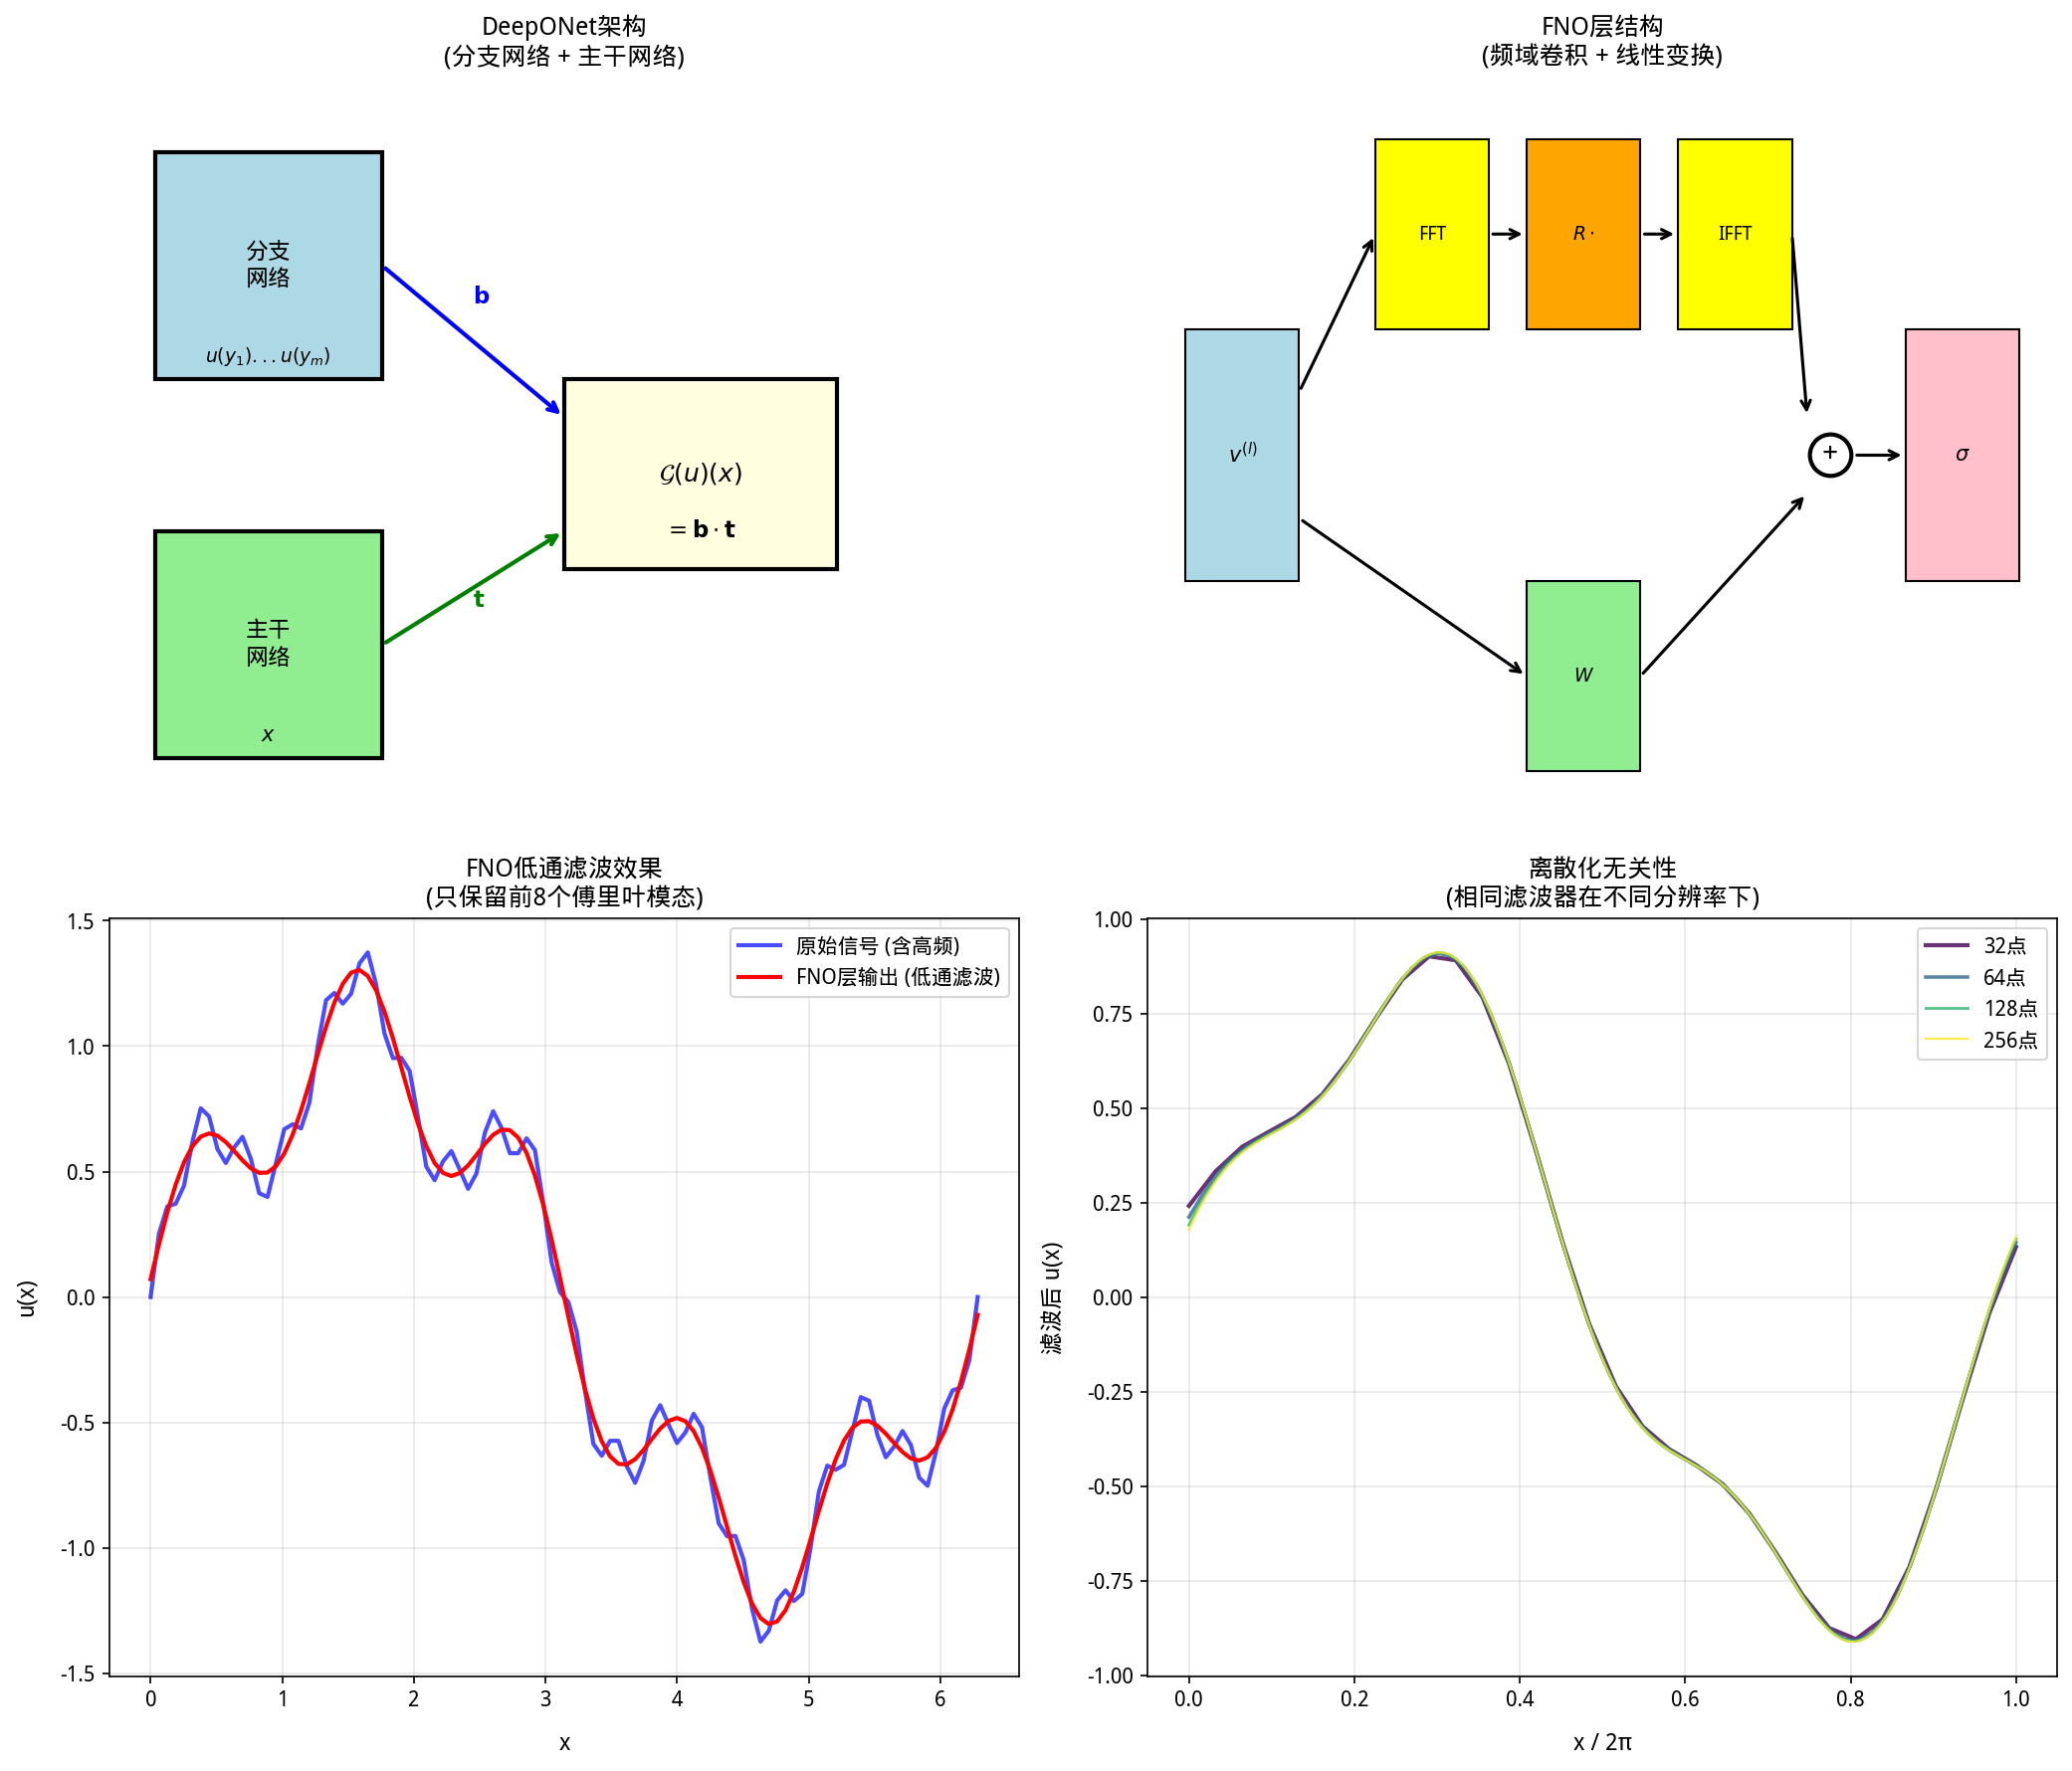
\includegraphics[width=0.95\textwidth]{figs_chap14/chap14_fig1.png}
\caption{神经算子概念演示。（1）DeepONet架构：分支网络处理输入函数采样值，主干网络处理查询位置，输出通过内积合成——这是万能逼近定理的实现；（2）FNO频域滤波：在傅里叶空间对高频和低频分量进行不同处理，体现频域操作的离散化无关性；（3）离散化无关性验证：同一个算子在不同分辨率网格上的输出保持一致性，实现零样本超分辨率的关键特性。}
\label{fig:chap14_neural_operator}
\end{figure}

% ====================================================================================
\section{本章小结}
% ====================================================================================

\begin{enumerate}
    \item \textbf{从函数到算子}：PINN 学一个特定问题的解 $u(x)$；神经算子学"条件函数 $\to$ 解函数"的映射 $\mathcal{G}$，一次训练、任意条件。
    \item \textbf{离散化无关性}：模型逼近的是连续算子，训练分辨率和推理分辨率可以不同（零样本超分辨率）。
    \item \textbf{数学统一}：所有神经算子都可以写成积分算子 $v(x) = \int \kappa(x, y) u(y)\,dy$，不同架构只是参数化积分核 $\kappa$ 的不同方式；线性情形下这个核就是格林函数，也就是第6章 $K^{-1}$ 的连续版本。
    \item \textbf{两种主流架构}：DeepONet（基函数展开：分支网络给系数、主干网络给基函数，理论清晰、通用）与 FNO（频域卷积：效率高、分辨率无关，适合周期 / 光滑问题）。
    \item \textbf{与 PINN 的关系}：PINN 把物理约束写进损失、针对单个问题；神经算子把物理隐含在数据里、针对一类问题；PINO 把两者结合。
\end{enumerate}

\begin{physicalmeaning}
\textbf{$\lambda$ 在本章的意义}：第1章的 $\lambda$ 回答"这条约束放松一点，目标变多少"；PDE 是一整族约束——每个点 $\xi$ 处方程都要成立——于是影子价格也成了一个函数：在 $\xi$ 处加一个单位源，解在 $x$ 处变化 $G(x, \xi)$。格林函数就是 PDE 约束的影子价格表，第9章的伴随变量就是这张表乘上目标的梯度。神经算子学的就是这张表。代价也在这里：纯数据驱动的 DeepONet / FNO 没有显式约束，$\lambda \equiv 0$，没有人替物理定律"看门"——这就是"应用案例"一节警告"预测可能违反守恒律"的根源；PINO 把第13章的乘子请回来，正是为了补上这个缺口。
\end{physicalmeaning}

% ====================================================================================
\section{习题}
% ====================================================================================

\paragraph{计算题}
\begin{enumerate}
    \item \textbf{格林函数与DeepONet}：
    考虑一维泊松方程$-u''(x) = f(x)$，$u(0) = u(1) = 0$。
    
    \begin{enumerate}
        \item 写出格林函数$G(x, y)$的表达式
        \item 如果用DeepONet学习从$f$到$u$的映射，分支网络的输入是什么？主干网络的输入是什么？
        \item DeepONet学到的$\sum_k b_k(f) t_k(x)$与格林函数表示$\int G(x,y) f(y) dy$有什么联系？
    \end{enumerate}
    
\end{enumerate}

\paragraph{编程题}
\begin{enumerate}
    \setcounter{enumi}{1}
    \item \textbf{实现2D FNO}：
    将本章的1D FNO代码扩展到2D情况：
    \begin{enumerate}
        \item 实现\code{SpectralConv2d}类
        \item 实现\code{FNO2d}类
        \item 在Darcy流问题上测试：给定渗透率场$a(x,y)$，预测压力场$u(x,y)$
    \end{enumerate}
    
    \textbf{提示}：2D FFT使用\code{torch.fft.rfft2}和\code{torch.fft.irfft2}。
    
    \item \textbf{DeepONet变体}：
    实现以下DeepONet的变体，并比较它们的性能：
    \begin{enumerate}
        \item \textbf{PI-DeepONet}：在损失函数中加入物理约束
        \item \textbf{Multi-output DeepONet}：主干网络输出多个查询点的结果
        \item \textbf{Deep DeepONet}：在内积之后再加一个MLP
    \end{enumerate}
    
\end{enumerate}

\paragraph{思考题}
\begin{enumerate}
    \setcounter{enumi}{3}
    \item \textbf{理解离散化无关性}：
    解释为什么以下操作不具有离散化无关性：
    \begin{enumerate}
        \item 全连接层 $y = Wx + b$，其中$x \in \mathbb{R}^n$
        \item 固定大小的卷积核
    \end{enumerate}
    
    提出一种使它们具有离散化无关性的修改方案。
    
    \item \textbf{神经算子的局限}：
    讨论神经算子在以下场景中可能遇到的困难：
    \begin{enumerate}
        \item 激波问题（Burgers方程在黏性趋近于零时）
        \item 湍流（高雷诺数Navier-Stokes方程）
        \item 多尺度问题（例如大气-海洋耦合）
    \end{enumerate}
    
    你能想到什么改进方法？
    
    \item \textbf{算子学习 vs 传统数值方法}：
    比较神经算子和传统数值方法（如有限元）的优缺点。在什么情况下应该选择神经算子？在什么情况下应该坚持传统方法？
    
\end{enumerate}
  % 第14章：算子学习
% ====================================================================================
\chapter{多智能体系统：从微观博弈到宏观平均场}
% ====================================================================================

% ====================================================================================
\section*{引言：当优化遇到博弈}
% ====================================================================================

\storynote{John Nash}{1928--2015，普林斯顿数学博士，21岁（1950年）就证明了纳什均衡的存在性。患精神分裂症数十年后奇迹康复，1994年获诺贝尔经济学奖。他的故事被拍成电影《美丽心灵》(A Beautiful Mind)，获奥斯卡最佳影片。2015年与妻子在出租车事故中去世。}

\storynote{John von Neumann}{1903--1957，20世纪最伟大的数学家之一，博弈论奠基人。他还发明了冯·诺伊曼计算机架构、参与曼哈顿计划、创立量子力学数学基础。据说他能用心算积分，智商估计超过180。}

在前面的章节中，我们一直在解决"一个智能体对抗环境"的问题：
\begin{itemize}
    \item 最优控制：一个控制器操控一个动力系统
    \item 强化学习：一个智能体在环境中最大化累积奖励
    \item PINN/神经算子：求解一个固定的PDE
\end{itemize}

但真实世界远比这复杂。想象以下场景：

\begin{quote}
\textit{早高峰时，每个司机都想选择最快的路线。但"最快"取决于其他人的选择——如果大家都选同一条路，这条路反而最慢。}
\end{quote}

\begin{quote}
\textit{在电力市场中，每个发电厂都想最大化利润。但电价取决于所有发电厂的总供应量——你的最优策略取决于别人怎么做。}
\end{quote}

\begin{quote}
\textit{一群无人机需要协作完成搜索任务。每架无人机的最优路径取决于其他无人机去哪里——你不想和别人重复搜索同一区域。}
\end{quote}

这些问题的共同特点是：\textbf{我的最优决策取决于你的决策，而你的最优决策也取决于我的决策}。

这就是\textbf{博弈论}（Game Theory）的领域。

\vspace{0.3cm}
\noindent\textit{为什么给城市多修一条路，反而可能让所有人都更堵？为什么"每个人都最优"和"整体最优"不是一回事？为什么当人多到数不清时，博弈论会变成流体力学？}

\begin{quote}
\textbf{本章目标}：当决策者不止一个时，"最优"这个词本身就要重新定义。本章要让你看到：纳什均衡不是新数学，而是把第1章的 KKT 条件同时写 $N$ 份；看似混乱的交通、市场和无人机群，背后常常藏着一个大家在共同最小化的势函数；而当玩家多到数不清时，博弈会自然地变成一对前向--后向的偏微分方程。
\end{quote}

\begin{tcolorbox}[colback=green!5, colframe=green!60!black, title=学完这章，你将能够...]
\begin{itemize}
    \item 用KKT条件计算简单博弈的纳什均衡
    \item 分析交通流量分配中的Wardrop均衡
    \item 理解QMIX、MAPPO等多智能体RL算法的核心思想
    \item 解释平均场博弈如何将$N$体问题简化为连续极限
    \item 用拉格朗日方法分析带约束的博弈问题
\end{itemize}
\end{tcolorbox}

% ====================================================================================
\section{博弈论基础：从优化到均衡}
% ====================================================================================

\subsection{从单人优化到多人博弈}

\review{第1章}{KKT 条件：驻点、可行、乘子非负、互补松弛。本章要做的只是把它写 $N$ 遍——每个玩家一遍——再要求它们同时成立。}
回顾单人优化问题：
\begin{equation}
    \min_{x} f(x) \quad \text{s.t.} \quad g(x) \leq 0
\end{equation}

最优解$x^*$满足KKT条件。这里只有一个决策者，目标函数$f(x)$只依赖于自己的决策$x$。

现在考虑\textbf{两人博弈}：

\begin{definition}[二人博弈]
一个二人博弈由以下元素组成：
\begin{itemize}
    \item \textbf{玩家1的策略空间}$\mathcal{A}_1$：玩家1可以选择的所有策略的集合
    \item \textbf{玩家2的策略空间}$\mathcal{A}_2$：玩家2可以选择的所有策略的集合
    \item \textbf{玩家1的代价函数}$J_1(a_1, a_2)$：玩家1要最小化的目标，\textbf{同时依赖于双方的策略}
    \item \textbf{玩家2的代价函数}$J_2(a_1, a_2)$：玩家2要最小化的目标，同样依赖于双方的策略
\end{itemize}
\end{definition}

\begin{remark}[与优化问题的关键区别]
在单人优化中，目标函数$f(x)$只依赖于决策者自己的选择$x$。但在博弈中，$J_1(a_1, a_2)$不仅依赖于玩家1的选择$a_1$，还依赖于玩家2的选择$a_2$。这意味着：
\begin{itemize}
    \item 玩家1想最小化$J_1$，但他控制不了$a_2$
    \item 玩家2想最小化$J_2$，但他控制不了$a_1$
    \item 双方的决策相互影响，形成一个"耦合"的系统
\end{itemize}
\end{remark}

每个玩家都想最小化自己的代价，但代价取决于对方的选择。这就产生了一个根本性的问题：

\begin{quote}
\textit{什么是"好"的策略组合？}
\end{quote}

\subsection{纳什均衡：没有人想单方面改变}
\review{第2章}{你其实已经见过纳什均衡：第2章把拉格朗日函数看成 $x$ 与 $\lambda$ 的零和博弈，强对偶成立时的鞍点 $(x^*, \lambda^*)$ 就是一个纳什均衡。}

\begin{definition}[纳什均衡]
策略组合$(a_1^*, a_2^*)$是一个\textbf{纳什均衡}（Nash Equilibrium），如果：
\begin{align}
    J_1(a_1^*, a_2^*) &\leq J_1(a_1, a_2^*), \quad \forall a_1 \in \mathcal{A}_1 \\
    J_2(a_1^*, a_2^*) &\leq J_2(a_1^*, a_2), \quad \forall a_2 \in \mathcal{A}_2
\end{align}
即：给定对方的策略，没有人能通过单方面改变自己的策略来降低代价。
\end{definition}

\begin{remark}[纳什均衡的直观理解]
让我们用更通俗的语言解释纳什均衡：

想象你和朋友在玩一个游戏。如果你们达到了纳什均衡状态，那意味着：
\begin{itemize}
    \item 你看了朋友的策略后，觉得"我现在的选择已经是最好的了，换别的只会更差"
    \item 你的朋友看了你的策略后，也觉得"我现在的选择已经是最好的了"
    \item 双方都没有动力去改变，系统达到一种"稳定"状态
\end{itemize}

\textbf{关键词}：单方面。纳什均衡不是说大家都开心，而是说没人想\textbf{单独}改变。
\end{remark}

\begin{example}[囚徒困境——博弈论最经典的例子]
\label{ex:prisoners}
两个囚犯分别被审讯，每人可以选择"合作"（保持沉默）或"背叛"（揭发对方）。

\textbf{变量含义}：
\begin{itemize}
    \item $a_1 \in \{\text{合作}, \text{背叛}\}$：玩家1的策略
    \item $a_2 \in \{\text{合作}, \text{背叛}\}$：玩家2的策略
    \item $J_1(a_1, a_2)$：玩家1的刑期（年），希望越小越好
    \item $J_2(a_1, a_2)$：玩家2的刑期（年），希望越小越好
\end{itemize}

代价矩阵（刑期）如下：

\begin{center}
\begin{tabular}{c|cc}
& 玩家2合作 & 玩家2背叛 \\
\hline
玩家1合作 & (1年, 1年) & (3年, 0年) \\
玩家1背叛 & (0年, 3年) & (2年, 2年) \\
\end{tabular}
\end{center}

\textbf{如何解读这个表格}：
\begin{itemize}
    \item 如果双方都合作（保持沉默），证据不足，各判1年
    \item 如果你背叛而对方合作，你当污点证人获释（0年），对方被重判（3年）
    \item 如果双方都背叛，各判2年
\end{itemize}

\textbf{分析纳什均衡}——我们来做"最优响应分析"：

\textit{假设玩家2选择合作}：
\begin{itemize}
    \item 玩家1选合作：刑期1年
    \item 玩家1选背叛：刑期0年 $\leftarrow$ \textbf{更好！}
\end{itemize}

\textit{假设玩家2选择背叛}：
\begin{itemize}
    \item 玩家1选合作：刑期3年
    \item 玩家1选背叛：刑期2年 $\leftarrow$ \textbf{更好！}
\end{itemize}

结论：\textbf{无论玩家2怎么选，玩家1选背叛总是更好}。这叫做"背叛是玩家1的\textbf{占优策略}"。

由于博弈是对称的，玩家2也会得出同样结论。

因此，\textbf{（背叛，背叛）是唯一的纳什均衡}，双方各判2年。

\textbf{悖论所在}：如果双方都选合作，各判1年，明明对双方都更好！但理性的个体不会选择合作，因为背叛总是对自己更有利。

这揭示了博弈论的一个深刻洞察：\textbf{个体理性不一定导致集体理性}。
\end{example}
\think{如果两人可以事先签一份"背叛者赔付 3 年"的合同，代价矩阵会怎样变？新的纳什均衡在哪里？（提示：合同就是一条新约束。）}

\begin{figure}[htbp]
\centering
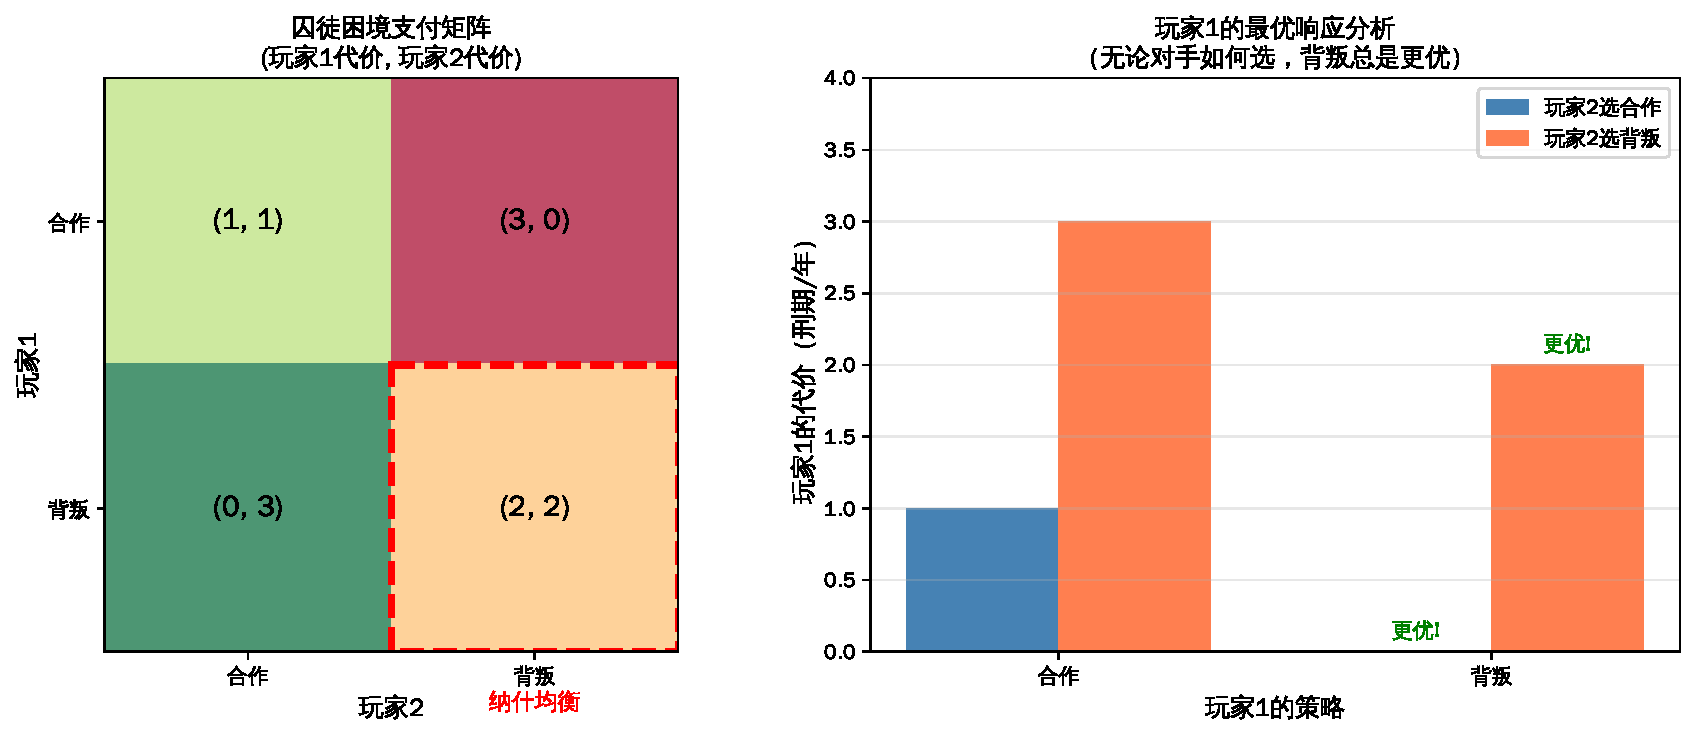
\includegraphics[width=0.95\textwidth]{figs_chap15/prisoners_dilemma.pdf}
\caption{囚徒困境的可视化分析。左图：支付矩阵热力图，红色虚线框标记纳什均衡（背叛，背叛）。右图：玩家1的最优响应分析，无论玩家2如何选择，背叛都是玩家1的更优选择。}
\label{fig:prisoners}
\end{figure}

图\ref{fig:prisoners}展示了囚徒困境的两种分析视角。从右图可以清楚看到：不管对手选什么，选择背叛总能让自己的代价更低。这就是为什么理性的玩家会陷入（背叛，背叛）的均衡，尽管（合作，合作）对双方都更好。

\subsection{连续策略博弈与最优响应}

当策略空间是连续的（如$\mathcal{A}_i = \R$），我们可以用微积分来分析。

\begin{definition}[最优响应]
给定对手的策略$a_{-i}$，玩家$i$的\textbf{最优响应}（Best Response）是：
\begin{equation}
    BR_i(a_{-i}) = \arg\min_{a_i \in \mathcal{A}_i} J_i(a_i, a_{-i})
\end{equation}

\textbf{直观理解}：如果我知道对手会选$a_{-i}$，我应该选什么来最小化自己的代价？答案就是$BR_i(a_{-i})$。
\end{definition}

\begin{proposition}[纳什均衡的不动点特征]
$(a_1^*, a_2^*)$是纳什均衡，当且仅当：
\begin{equation}
    a_1^* = BR_1(a_2^*), \quad a_2^* = BR_2(a_1^*)
\end{equation}
即每个人的策略都是对方策略的最优响应。
\end{proposition}

\begin{remark}[不动点的直观含义]
这个条件说的是：在纳什均衡点，形成了一个"自洽"的循环：
\begin{itemize}
    \item 玩家1选$a_1^*$是因为对手选了$a_2^*$
    \item 玩家2选$a_2^*$是因为对手选了$a_1^*$
    \item 谁也不想先改变，因为改变只会让自己更差
\end{itemize}

这正是数学中"不动点"的概念：$x^* = f(x^*)$，即函数作用在某个点上还是它自己。
\end{remark}

这给出了一个寻找纳什均衡的算法思路：\textbf{迭代最优响应}（Iterated Best Response）。

\begin{algorithm}
\caption{迭代最优响应（伪代码）}
\begin{algorithmic}[1]
\State \textbf{输入}: 初始策略 $a_1^{(0)}, a_2^{(0)}$，迭代次数 $K$
\State \textbf{输出}: 近似纳什均衡 $(a_1^{(K)}, a_2^{(K)})$
\For{$k = 0, 1, 2, \ldots, K-1$}
    \State $a_1^{(k+1)} \leftarrow BR_1(a_2^{(k)})$ \Comment{玩家1对玩家2当前策略的最优响应}
    \State $a_2^{(k+1)} \leftarrow BR_2(a_1^{(k+1)})$ \Comment{玩家2对玩家1新策略的最优响应}
\EndFor
\State \Return $(a_1^{(K)}, a_2^{(K)})$
\end{algorithmic}
\end{algorithm}

\begin{warning}[title=迭代最优响应不一定收敛]
迭代最优响应可能：
\begin{itemize}
    \item \textbf{收敛到纳什均衡}（如果博弈是"好"的）
    \item \textbf{陷入循环}（如石头剪刀布）
    \item \textbf{发散}
\end{itemize}
收敛性取决于博弈的结构，我们稍后会看到一类保证收敛的"势博弈"。
\end{warning}
\preview{下一节的 Beckmann 势函数就是这样的例子：每个司机各自为政，宏观上却在最小化同一个凸函数 $\Phi$——博弈又变回了第1章的优化。}

% ====================================================================================
\section{物理约束下的静态博弈}
% ====================================================================================

\begin{tcolorbox}[colback=yellow!10, colframe=orange!80, title=本章的核心观点]
\textbf{本章的问题就是第1章的拉格朗日乘子法，只是要同时写 $N$ 份——每个玩家一份，各自只对自己的变量求导，却共享同一组变量。}

这不是比喻：广义纳什均衡的定义，就是"$N$ 组 KKT 条件同时成立"。

\begin{center}
\renewcommand{\arraystretch}{1.3}
\small
\begin{tabular}{lll}
\toprule
\textbf{概念} & \textbf{第1章（单人优化）} & \textbf{本章（博弈）} \\
\midrule
变量 & 一个向量 $x$ & $N$ 个玩家各自的 $a_i$，合起来 $(a_1, \ldots, a_N)$ \\
目标 & 一个 $f(x)$ & $N$ 个 $J_i(a_i, a_{-i})$，玩家 $i$ 只管自己的 \\
约束 & $g(x) \le 0$ & $g_i(a_i, a_{-i}) \le 0$，可能依赖别人的选择 \\
乘子 & $\lambda$：影子价格 & 每人一组 $\lambda_i$；Wardrop 中 $\lambda_w$ = 均衡旅行时间 \\
一阶条件 & 一组 KKT & $N$ 组 KKT 同时成立 $=$ 广义纳什均衡 \\
特例 & --- & 势博弈：$N$ 组 KKT 恰好是同一个 $\Phi$ 的一组 KKT \\
\bottomrule
\end{tabular}
\end{center}
\end{tcolorbox}

\subsection{广义纳什均衡与KKT条件}

在实际问题中，每个玩家的策略通常受到\textbf{物理约束}：
\begin{itemize}
    \item 能量上限：$\|a_i\|^2 \leq E_{\max}$
    \item 位置限制：$a_i \in [0, L]$
    \item 资源预算：$c^T a_i \leq B$
\end{itemize}

\begin{definition}[广义纳什均衡问题]
$N$个玩家的\textbf{广义纳什均衡问题}（Generalized Nash Equilibrium Problem, GNEP）：

每个玩家$i$求解：
\begin{equation}
    \min_{a_i} J_i(a_i, a_{-i}) \quad \text{s.t.} \quad g_i(a_i, a_{-i}) \leq 0
\end{equation}

\textbf{变量说明}：
\begin{itemize}
    \item $a_i$：玩家$i$的策略（决策变量）
    \item $a_{-i}$：除玩家$i$外所有其他玩家的策略
    \item $J_i$：玩家$i$的代价函数
    \item $g_i$：玩家$i$面临的约束（可能依赖于其他玩家的策略）
\end{itemize}
\end{definition}

\begin{keyinsight}
纳什均衡可以用\textbf{KKT条件系统}来刻画！

在纳什均衡$(a_1^*, \ldots, a_N^*)$处，每个玩家$i$的策略$a_i^*$必须满足其优化问题的KKT条件：
\begin{align}
    \nabla_{a_i} J_i(a_i^*, a_{-i}^*) + \sum_j \lambda_{ij}^* \nabla_{a_i} g_{ij}(a_i^*, a_{-i}^*) &= 0 \quad \text{（驻点条件）} \\
    \lambda_{ij}^* &\geq 0 \quad \text{（乘子非负）} \\
    \lambda_{ij}^* g_{ij}(a_i^*, a_{-i}^*) &= 0 \quad \text{（互补松弛）} \\
    g_{ij}(a_i^*, a_{-i}^*) &\leq 0 \quad \text{（可行性）}
\end{align}

这是$N$组KKT条件\textbf{同时成立}！
\end{keyinsight}
\clarify{单人优化是"一个目标、一组 KKT"；博弈是"$N$ 个目标、$N$ 组 KKT"，它们共享变量，却各自只对自己的 $a_i$ 求导。所以均衡一般不是任何一个函数的极小点——除非它是势博弈。}

\begin{remark}[KKT条件的物理意义]
回忆一下KKT条件的含义：
\begin{itemize}
    \item \textbf{驻点条件}：在最优点，目标函数的梯度被约束的梯度"抵消"了
    \item \textbf{互补松弛}：约束要么不起作用（$g < 0$），要么起作用但乘子为正（$\lambda > 0$）
\end{itemize}

在博弈中，每个玩家都在自己的约束下做优化，所以每个人的KKT条件都要满足。纳什均衡就是这$N$组条件的公共解。
\end{remark}

\subsection{案例一：图博弈——邻居之间的互动}

\begin{definition}[图博弈]
在\textbf{图博弈}（Network Game）中：
\begin{itemize}
    \item 玩家位于图$G = (V, E)$的节点上
    \item 玩家$i$的代价只依赖于自己和\textbf{邻居}的策略：
    \begin{equation}
        J_i(a_i, a_{N(i)}) = f_i(a_i) + \sum_{j \in N(i)} \phi_{ij}(a_i, a_j)
    \end{equation}
    其中$N(i)$是$i$的邻居集合
\end{itemize}
\end{definition}

\begin{example}[线性二次图博弈——一个完整的求解过程]
\label{ex:lq_network}
考虑代价函数：
\begin{equation}
    J_i = \frac{1}{2}(a_i - a_{i,0})^2 + \delta \cdot a_i \sum_{j \in N(i)} a_j
\end{equation}

\textbf{变量含义详解}：
\begin{itemize}
    \item $a_i \in \R$：玩家$i$的策略/行动（比如生产量、投入的努力等）
    \item $a_{i,0}$：玩家$i$的"理想状态"或"目标值"（如果没有邻居影响，他想选择的值）
    \item $\delta$：交互强度参数，决定邻居对你的影响有多大
    \item $N(i)$：玩家$i$的邻居集合（图中与$i$相连的节点）
\end{itemize}

\textbf{代价函数的物理解释}：
\begin{itemize}
    \item \textbf{第一项} $(a_i - a_{i,0})^2/2$：偏离理想状态的代价。你想待在$a_{i,0}$附近，离得越远代价越大
    \item \textbf{第二项} $\delta \cdot a_i \sum_{j \in N(i)} a_j$：与邻居的交互代价
    \begin{itemize}
        \item 如果$\delta > 0$（\textbf{策略替代}）：邻居做得多，你做得多会增加代价。类似于竞争关系——市场上对手生产越多，你再多生产就越亏
        \item 如果$\delta < 0$（\textbf{策略互补}）：邻居做得多，你做得多反而减少代价。类似于协作关系——朋友都在学习，你学习效果也更好
    \end{itemize}
\end{itemize}

\textbf{求解纳什均衡}：

每个玩家$i$想最小化$J_i$，将$a_i$视为决策变量，$a_{-i}$视为已知。

对$a_i$求导并令其为零（一阶最优性条件）：
\begin{equation}
    \frac{\partial J_i}{\partial a_i} = (a_i - a_{i,0}) + \delta \sum_{j \in N(i)} a_j = 0
\end{equation}

解这个方程得到\textbf{最优响应}：
\begin{equation}
    a_i^* = a_{i,0} - \delta \sum_{j \in N(i)} a_j^*
\end{equation}

\textbf{解读}：如果$\delta > 0$（竞争），邻居行动越大，你的最优响应越小。如果$\delta < 0$（协作），邻居行动越大，你也应该行动更大。

\textbf{矩阵形式}：

把所有$N$个玩家的最优响应方程写在一起：
\begin{equation}
    \mathbf{a}^* = \mathbf{a}_0 - \delta A \mathbf{a}^*
\end{equation}
其中$A$是图的邻接矩阵：$A_{ij} = 1$如果$i$和$j$是邻居，否则为0。

移项整理：
\begin{equation}
    (I + \delta A) \mathbf{a}^* = \mathbf{a}_0
\end{equation}

解得纳什均衡：
\begin{equation}
    \boxed{\mathbf{a}^* = (I + \delta A)^{-1} \mathbf{a}_0}
\end{equation}

这是一个漂亮的闭式解！只需要知道图结构（邻接矩阵$A$）和每个人的理想状态（$\mathbf{a}_0$），就能直接算出均衡。
\tryit{用 NumPy 构造 6 节点环形图的邻接矩阵，分别取 $\delta = 0.15$ 和 $\delta = 0.6$ 计算 $(I + \delta A)^{-1}\mathbf{a}_0$，再跑迭代最优响应。哪个 $\delta$ 下迭代发散？和 $A$ 的谱半径比一比。}
\end{example}

\begin{figure}[htbp]
\centering
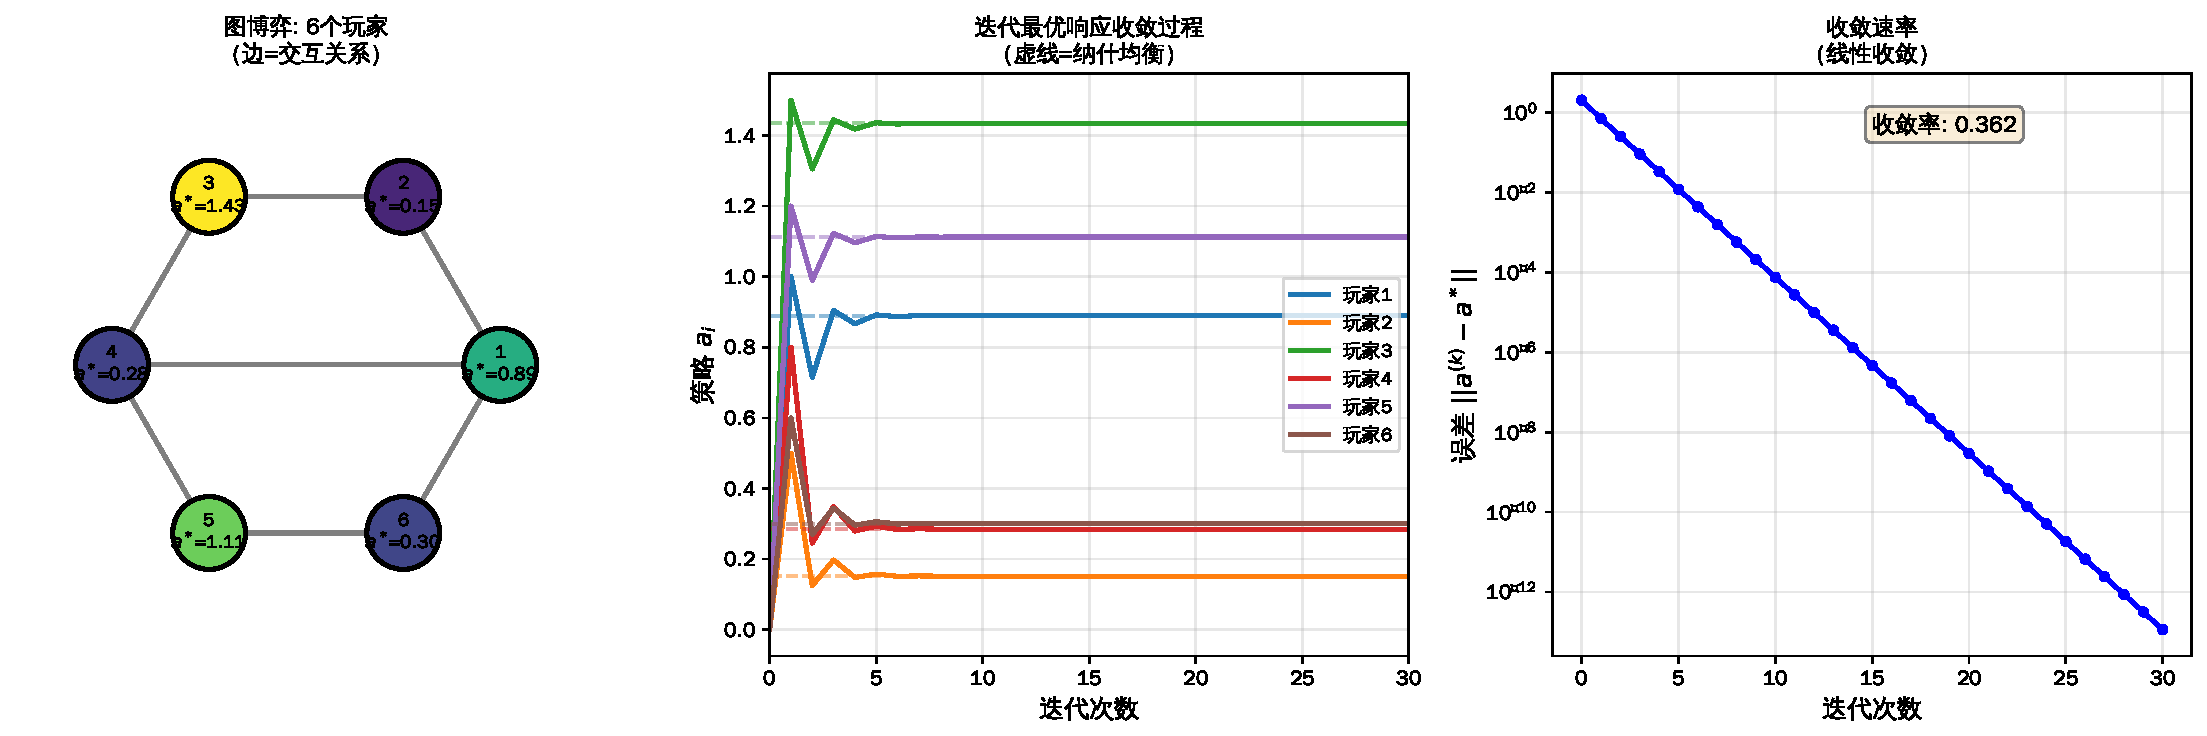
\includegraphics[width=0.95\textwidth]{figs_chap15/network_game.pdf}
\caption{图博弈的数值实验。左图：6个玩家组成的网络，节点颜色表示均衡策略的大小。中图：迭代最优响应过程，从零初始化出发，每个玩家的策略逐渐收敛到纳什均衡（虚线）。右图：收敛误差随迭代次数呈指数下降，表明算法线性收敛。参数：$\delta = 0.15$（策略替代）。}
\label{fig:network_game}
\end{figure}

图\ref{fig:network_game}展示了图博弈的实际计算结果。可以观察到：
\begin{itemize}
    \item 迭代最优响应算法确实收敛到了纳什均衡
    \item 收敛速度是\textbf{线性}的（在对数坐标下误差直线下降）
    \item 不同位置的玩家（中心节点vs边缘节点）有不同的均衡策略
\end{itemize}

\subsection{案例二：交通均衡与Braess悖论}

\begin{example}[Wardrop交通均衡]
\label{ex:wardrop}
考虑一个交通网络：
\begin{itemize}
    \item $W$个OD对（Origin-Destination，起点-终点对）
    \item 每个OD对$w$有需求$d_w$（单位时间内要从起点到终点的车辆数）
    \item 每个OD对有多条可选路径$P_w$
    \item 每条边$a$有时间函数$t_a(x_a)$，其中$x_a$是边$a$的流量
\end{itemize}

\textbf{Wardrop第一原理}（用户均衡）：在均衡状态下，每个OD对所有被使用的路径具有\textbf{相同且最小}的旅行时间。

\textbf{直观理解}：如果有一条更快的路，司机会切换过去。切换的人多了，那条路就变慢了。最终达到平衡：所有在用的路一样快，没人想换。
\end{example}

\begin{example}[Braess悖论——增加道路反而更堵！]
\label{ex:braess}
\storynote{Dietrich Braess}{德国数学家（1938--）。1968 年他研究交通网络的数值方法时发现：给路网加一条边，可能让所有人的均衡旅行时间变长。这篇德语论文沉寂多年，直到规划者在纽约、首尔的真实道路上看到同样现象才广为人知。}
这是交通领域最著名的悖论之一。考虑从起点S到终点E的交通网络：

\textbf{网络结构}：
\begin{itemize}
    \item 节点：S（起点）、A、B、E（终点）
    \item 边SA：时间函数$t_{SA}(x) = x/100$（流量越大越慢）
    \item 边AE：固定时间$t_{AE} = 45$分钟
    \item 边SB：固定时间$t_{SB} = 45$分钟
    \item 边BE：时间函数$t_{BE}(x) = x/100$
    \item 边AB（Braess边）：时间$t_{AB} = 0$（\textbf{免费捷径！}）
\end{itemize}

总需求：4000辆车从S到E。

\textbf{情况1：没有AB边}

可选路径：
\begin{itemize}
    \item 路径1：S $\to$ A $\to$ E，时间 = $x_{SA}/100 + 45$
    \item 路径2：S $\to$ B $\to$ E，时间 = $45 + x_{BE}/100$
\end{itemize}

由对称性，均衡时各2000辆车：
\begin{itemize}
    \item 路径1时间：$2000/100 + 45 = 20 + 45 = 65$分钟
    \item 路径2时间：$45 + 2000/100 = 45 + 20 = 65$分钟 $\checkmark$
\end{itemize}

\textbf{所有人旅行时间：65分钟}

\textbf{情况2：有AB边（免费捷径）}

新增路径3：S $\to$ A $\to$ B $\to$ E，时间 = $x_{SA}/100 + 0 + x_{BE}/100$

\textbf{关键分析}：假设所有4000辆车都走路径3（S$\to$A$\to$B$\to$E）：
\begin{itemize}
    \item 路径3时间：$4000/100 + 0 + 4000/100 = 40 + 0 + 40 = 80$分钟
\end{itemize}

验证这是纳什均衡——有人想换路吗？
\begin{itemize}
    \item 换到路径1（S$\to$A$\to$E）：$40 + 45 = 85$分钟 > 80分钟，更差！
    \item 换到路径2（S$\to$B$\to$E）：$45 + 40 = 85$分钟 > 80分钟，更差！
\end{itemize}

没人想换，所以\textbf{所有人走S$\to$A$\to$B$\to$E确实是纳什均衡}。

\textbf{所有人旅行时间：80分钟}

\textbf{悖论}：增加了一条\textbf{免费}道路，所有人的旅行时间反而从65分钟增加到80分钟！增加了约23\%！

\textbf{为什么会这样？}
\begin{itemize}
    \item 免费捷径看起来很诱人
    \item 每个人都"理性"地选择它
    \item 但大家都这么想，导致SA和BE两条边都拥挤了
    \item 如果政府\textbf{禁止}这条免费道路，反而能让所有人更快到达！
\end{itemize}

这再次说明：\textbf{个体理性 $\neq$ 集体理性}。
\end{example}

\begin{figure}[htbp]
\centering
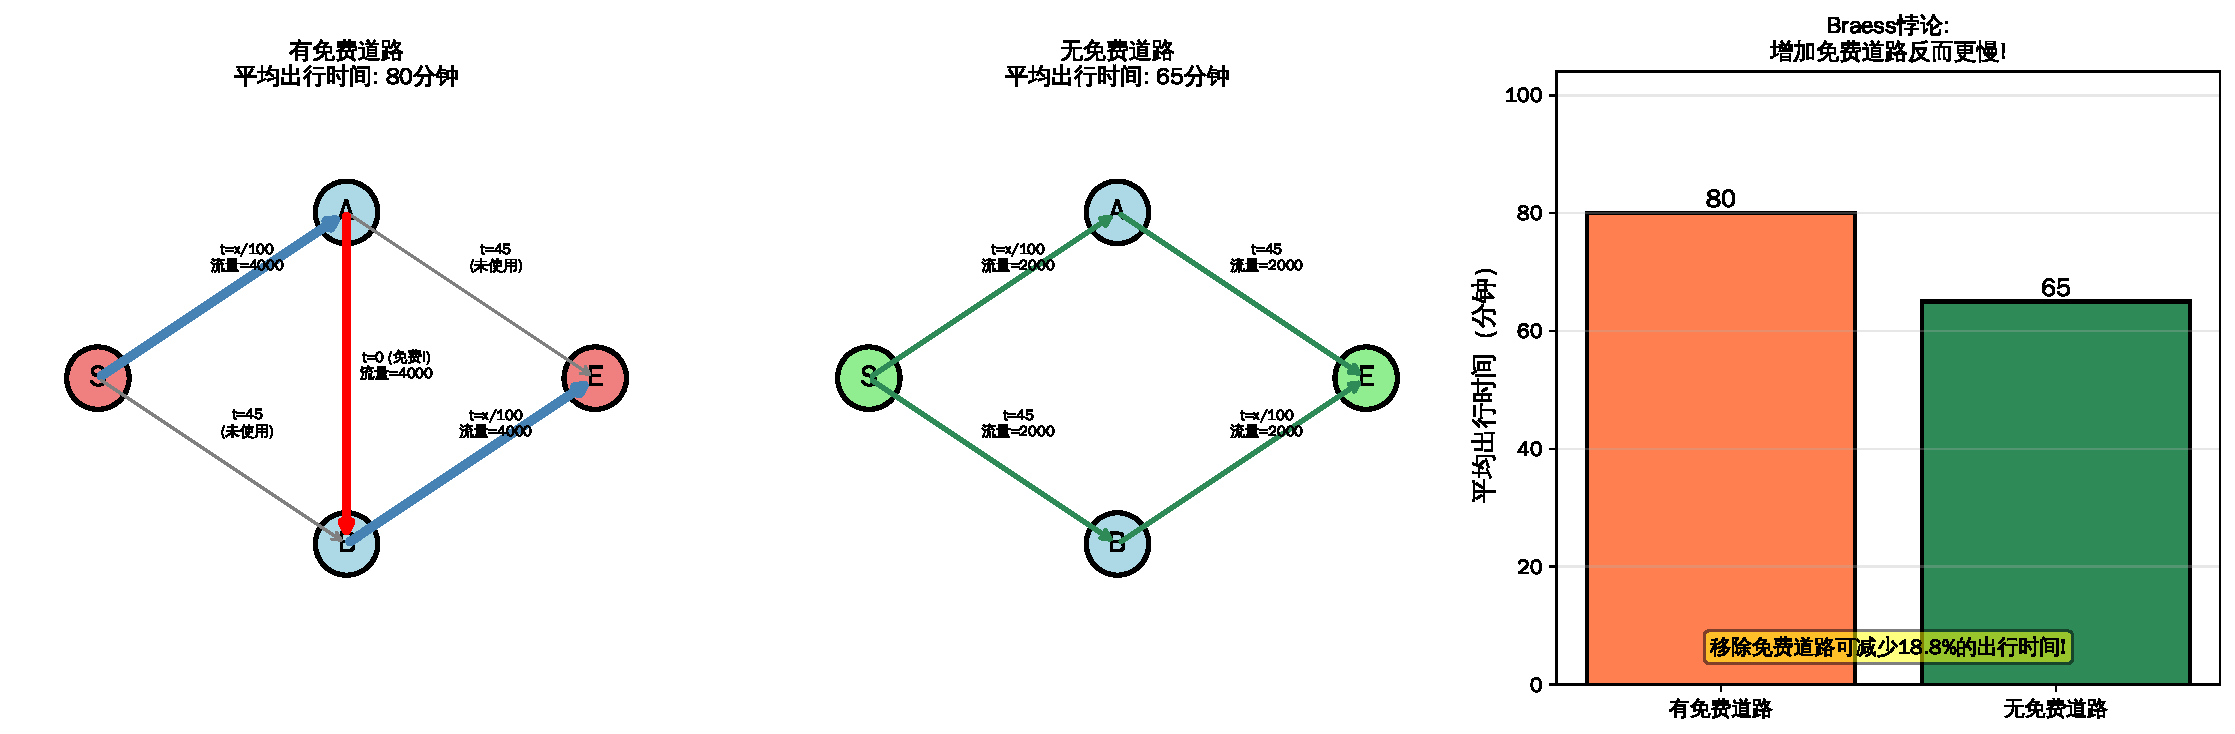
\includegraphics[width=0.95\textwidth]{figs_chap15/braess_paradox.pdf}
\caption{Braess悖论的数值验证。左图：有免费道路（红色AB边）时，所有车辆都选择S$\to$A$\to$B$\to$E路径，平均旅行时间80分钟。中图：没有免费道路时，车辆均匀分布在两条路径上，平均旅行时间65分钟。右图：柱状对比显示，移除免费道路可减少约18.8\%的旅行时间。}
\label{fig:braess}
\end{figure}

图\ref{fig:braess}直观展示了Braess悖论。这个悖论在现实中确实存在——1990年代，纽约市关闭了第42街的一段道路后，周围的交通状况反而改善了！首尔在2003年拆除了一条高架路后，交通拥堵也得到缓解。

\subsection{势博弈：自私博弈的隐藏秩序}

\begin{theorem}[Beckmann势函数]
如果边时间函数$t_a(x_a)$是连续且非递减的，则Wardrop用户均衡是以下\textbf{凸优化问题}的解：
\begin{equation}
    \min_{\mathbf{f}} \Phi(\mathbf{x}(\mathbf{f})) = \sum_{a} \int_0^{x_a} t_a(s) \, ds
\end{equation}
\begin{equation}
    \text{s.t.} \quad \sum_{p \in P_w} f_p = d_w, \quad f_p \geq 0, \quad x_a = \sum_{p \ni a} f_p
\end{equation}

\textbf{变量说明}：
\begin{itemize}
    \item $f_p$：路径$p$上的流量
    \item $x_a$：边$a$上的总流量（所有经过边$a$的路径流量之和）
    \item $d_w$：OD对$w$的总需求
    \item $\Phi$：Beckmann势函数
\end{itemize}
\end{theorem}

\begin{proof}[用KKT条件证明Wardrop均衡]
这是一个经典的``优化 $\Leftrightarrow$ 均衡''对应。让我们用KKT条件来证明Beckmann问题的解恰好满足Wardrop用户均衡条件。

\textbf{Step 1：写出拉格朗日函数}

对于路径流量$f_p$的约束优化问题，拉格朗日函数为：
\begin{equation}
    \mathcal{L} = \sum_{a} \int_0^{x_a} t_a(s) \, ds - \sum_w \lambda_w \left( \sum_{p \in P_w} f_p - d_w \right) - \sum_p \mu_p f_p
\end{equation}
其中：
\begin{itemize}
    \item $\lambda_w$：OD对$w$的需求约束的乘子
    \item $\mu_p \geq 0$：路径流量非负约束$f_p \geq 0$的乘子
\end{itemize}
（这里把 $f_p \ge 0$ 写成 $-f_p \le 0$，并用减号引入乘子；与第1章的 $\Lag = f + \lambda g + \mu h$ 只差记号约定。）

\textbf{Step 2：对$f_p$求偏导}

注意$x_a = \sum_{p \ni a} f_p$，所以$\frac{\partial x_a}{\partial f_p} = 1$（如果路径$p$经过边$a$）。因此：
\begin{equation}
    \frac{\partial \mathcal{L}}{\partial f_p} = \sum_{a \in p} t_a(x_a) - \lambda_w - \mu_p = 0
\end{equation}
即：\textbf{路径$p$的总旅行时间} = $\lambda_w + \mu_p$

\textbf{Step 3：互补松弛条件}

KKT的互补松弛条件要求：$\mu_p \cdot f_p = 0$
\begin{itemize}
    \item 若$f_p > 0$（路径被使用），则$\mu_p = 0$，故路径时间 $= \lambda_w$
    \item 若$f_p = 0$（路径未被使用），则$\mu_p \geq 0$，故路径时间 $\geq \lambda_w$
\end{itemize}

\textbf{Step 4：这正是Wardrop条件！}

上述结论可以总结为：
\begin{center}
\fbox{\parbox{0.8\textwidth}{
\textbf{所有被使用的路径}（$f_p > 0$）具有\textbf{相同的}旅行时间$\lambda_w$；\\
\textbf{所有未被使用的路径}（$f_p = 0$）旅行时间$\geq \lambda_w$。
}}
\end{center}

这正是Wardrop第一原理的数学表述！乘子$\lambda_w$就是OD对$w$的\textbf{均衡旅行时间}。
\end{proof}
\clarify{这正是第1章的影子价格：$\partial \Phi^*/\partial d_w = \lambda_w$，再多派一辆车走 OD 对 $w$，势函数恰好增加这辆车自己经历的旅行时间。它不等于系统总旅行时间的增量——后者还要加上这辆车给别人添的堵，两者之差 $x_a t_a'(x_a)$ 就是"拥堵费"。}

\begin{keyinsight}
\textbf{自私博弈的隐藏秩序}：

看似混乱的交通系统——每个司机都在自私地最小化自己的旅行时间——在宏观上却等价于在优化一个系统的``总势能''$\Phi$。

这类博弈被称为\textbf{势博弈}（Potential Game）：存在一个势函数$\Phi$，每个玩家改变策略导致的代价变化等于势函数的变化。

势博弈有很好的性质：
\begin{itemize}
    \item 纳什均衡一定存在（$\Phi$的最小值点）
    \item 最优响应动态一定收敛（因为$\Phi$单调下降）
    \item 可以用优化算法求解均衡
\end{itemize}
\end{keyinsight}

\begin{figure}[htbp]
\centering
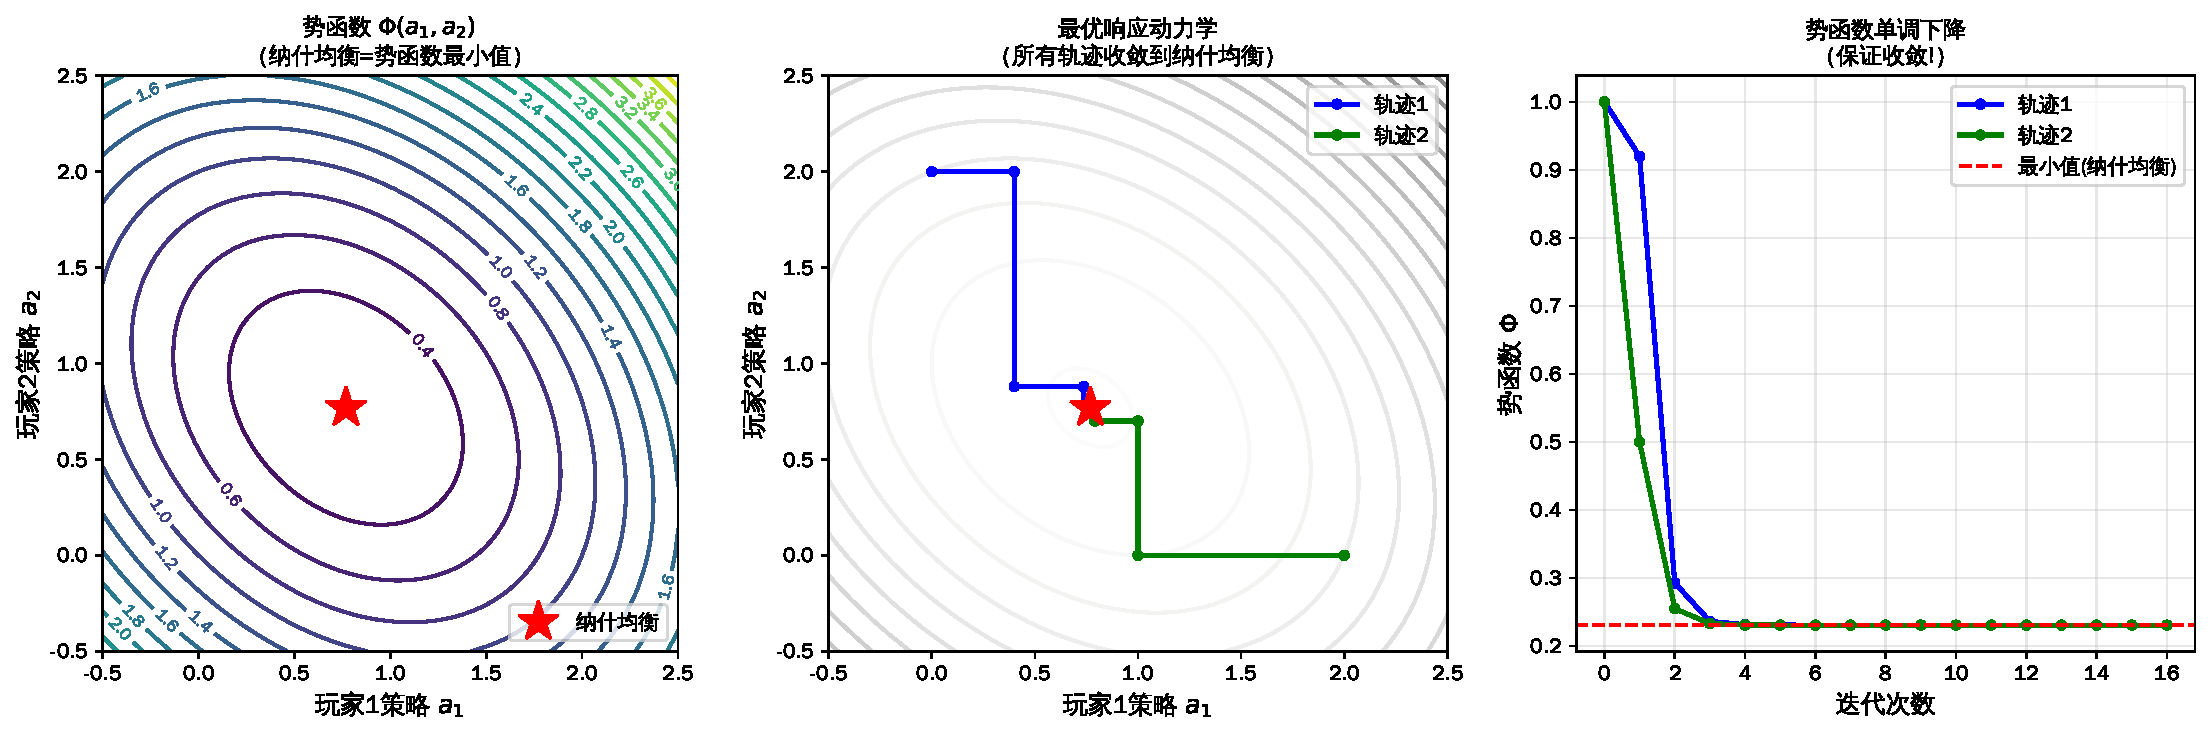
\includegraphics[width=0.95\textwidth]{figs_chap15/potential_game.pdf}
\caption{势博弈的收敛性质。左图：势函数$\Phi(a_1, a_2)$的等高线，红星标记纳什均衡（势函数最小值点）。中图：从不同初始点出发的迭代最优响应轨迹，都收敛到纳什均衡。右图：势函数沿轨迹单调下降，保证收敛性。}
\label{fig:potential}
\end{figure}

图\ref{fig:potential}展示了势博弈的核心性质：势函数沿着迭代最优响应的轨迹\textbf{单调下降}。这就像一个小球在山谷中滚动，总会滚到最低点（纳什均衡）。这也是为什么势博弈特别"好"——我们可以把博弈问题转化为优化问题来求解。

% ====================================================================================
\section{深度多智能体强化学习}
% ====================================================================================

前面我们讨论的都是\textbf{静态博弈}——玩家同时做出决策，博弈只进行一轮。

现在我们加入\textbf{时间}维度：智能体需要在多个时间步做出决策，当前决策会影响未来状态。这就是\textbf{动态博弈}，或更具体地说，\textbf{马尔可夫博弈}（Markov Game）。

\subsection{从静态到动态：马尔可夫博弈}

\begin{definition}[马尔可夫博弈]
一个$N$人\textbf{马尔可夫博弈}（又称随机博弈）由以下元素组成：
\begin{itemize}
    \item \textbf{状态空间}$\mathcal{S}$：系统可能处于的所有状态
    \item \textbf{动作空间}$\mathcal{A}_i$：每个智能体$i$可选择的动作
    \item \textbf{状态转移}$P(s' | s, a_1, \ldots, a_N)$：给定当前状态和所有人的动作，下一个状态的概率分布
    \item \textbf{奖励函数}$r_i(s, a_1, \ldots, a_N)$：每个智能体在每一步获得的即时奖励
    \item \textbf{折扣因子}$\gamma \in [0,1)$：未来奖励的折扣率
\end{itemize}

每个智能体$i$的目标是最大化累积奖励：
\begin{equation}
    \max_{\pi_i} \E\left[ \sum_{t=0}^{\infty} \gamma^t r_i(s_t, a_{1,t}, \ldots, a_{N,t}) \right]
\end{equation}
\end{definition}

\review{第10章}{第10章里 Q 学习、策略梯度的收敛性都假设转移概率固定。这里 $\pi_{-i}$ 在变，等于地基在动——单智能体的收敛保证从根上失效。}
\begin{warning}[title=多智能体RL的核心困难：非平稳性]
\textbf{问题}：从智能体$i$的视角看，环境的转移概率是：
\begin{equation}
    P(s' | s, a_i) = \sum_{a_{-i}} P(s' | s, a_i, a_{-i}) \pi_{-i}(a_{-i} | s)
\end{equation}

但其他智能体也在学习，所以$\pi_{-i}$在不断变化！

\textbf{后果}：
\begin{itemize}
    \item 环境对于单个智能体是\textbf{非平稳}的（规则在变）
    \item 单智能体RL的收敛性保证不再成立
    \item "追逐移动目标"问题——你刚学会应对对手的策略，对手又变了
\end{itemize}

\textbf{类比}：想象你在学下棋，但对手每天都在变强。你昨天赢他的策略，今天可能就不管用了。
\end{warning}

\subsection{CTDE范式：集中训练，分散执行}

解决非平稳性的一个关键思想是\textbf{CTDE}（Centralized Training with Decentralized Execution）：

\begin{itemize}
    \item \textbf{训练时}：可以使用全局信息（所有智能体的观测和动作）
    \item \textbf{执行时}：每个智能体只能使用自己的局部观测
\end{itemize}

\begin{figure}[htbp]
\centering
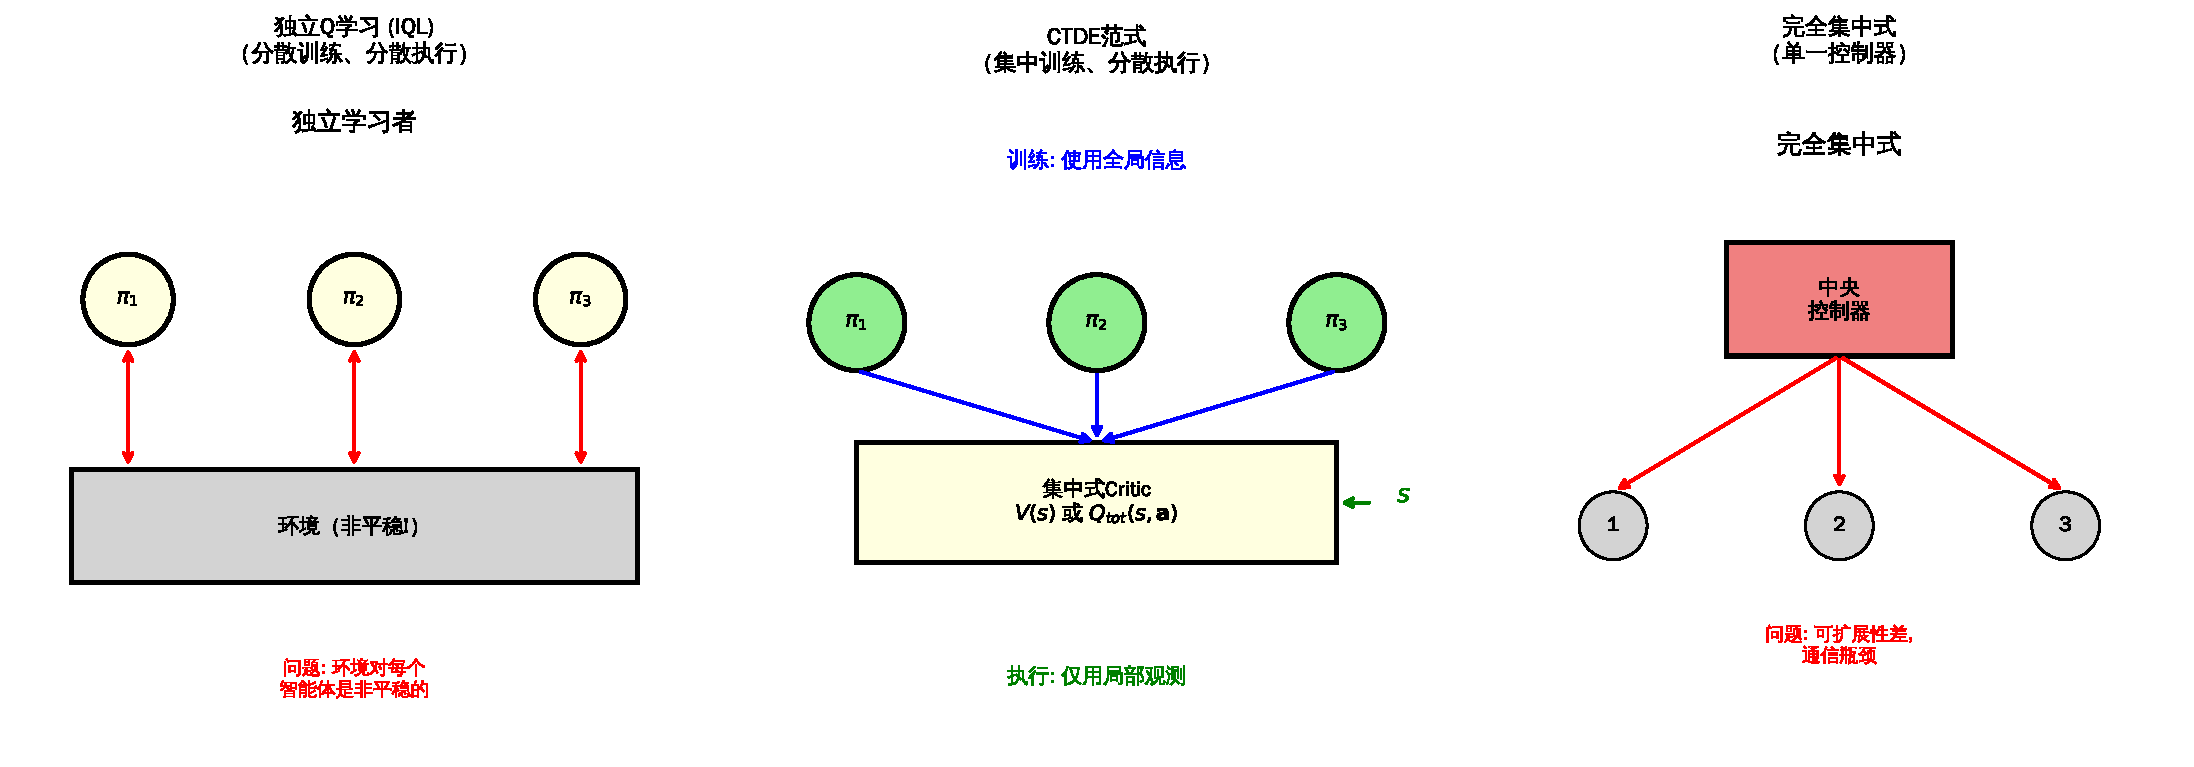
\includegraphics[width=0.95\textwidth]{figs_chap15/ctde_comparison.pdf}
\caption{三种多智能体学习范式的对比。左：独立学习（IQL），每个智能体独立与环境交互，面临非平稳性问题。中：CTDE范式，训练时使用全局信息（集中式Critic），执行时只用局部观测（分散式Actor）。右：完全集中式，由单一控制器指挥所有智能体，存在可扩展性和通信瓶颈问题。}
\label{fig:ctde}
\end{figure}

图\ref{fig:ctde}对比了三种学习范式。CTDE是目前最流行的方法，因为它在\textbf{训练效率}和\textbf{执行灵活性}之间取得了很好的平衡。

\subsection{价值分解方法：QMIX}

QMIX是CTDE范式下\textbf{价值分解}（Value Decomposition）方法的代表。

\begin{definition}[IGM原则——核心思想]
\textbf{IGM}（Individual-Global-Max）原则要求：
\begin{equation}
    \arg\max_{\mathbf{a}} Q_{tot}(s, \mathbf{a}) = \begin{pmatrix} \arg\max_{a_1} Q_1(o_1, a_1) \\ \vdots \\ \arg\max_{a_N} Q_N(o_N, a_N) \end{pmatrix}
\end{equation}

\textbf{直观理解}：最大化全局Q值的联合动作，等于每个智能体分别最大化自己局部Q值的动作组合。

\textbf{为什么重要}：这保证了分散执行的一致性——每个智能体贪婪地选择自己的最优动作，组合起来就是全局最优！
\end{definition}

\begin{theorem}[QMIX的单调性约束]
如果$Q_{tot}$关于每个$Q_i$是单调递增的：
\begin{equation}
    \frac{\partial Q_{tot}}{\partial Q_i} \geq 0, \quad \forall i
\end{equation}
则IGM原则自动满足。
\end{theorem}

\begin{proof}
设$a_i^* = \arg\max_{a_i} Q_i(o_i, a_i)$。

对于任意其他动作$a_i'$，有$Q_i(o_i, a_i^*) \geq Q_i(o_i, a_i')$。

由单调性（$Q_{tot}$ 对每个 $Q_i$ 非减），对任意联合动作 $a' = (a_1', \ldots, a_N')$，逐个坐标替换：
\begin{equation}
    Q_{tot}(s, a_1^*, a_2^*, \ldots, a_N^*) \geq Q_{tot}(s, a_1', a_2^*, \ldots, a_N^*) \geq Q_{tot}(s, a_1', a_2', \ldots, a_N^*) \geq \cdots \geq Q_{tot}(s, a')
\end{equation}
每一步只换一个坐标，用一次单调性。所以$(a_1^*, \ldots, a_N^*)$最大化$Q_{tot}$。
\end{proof}

\begin{figure}[htbp]
\centering
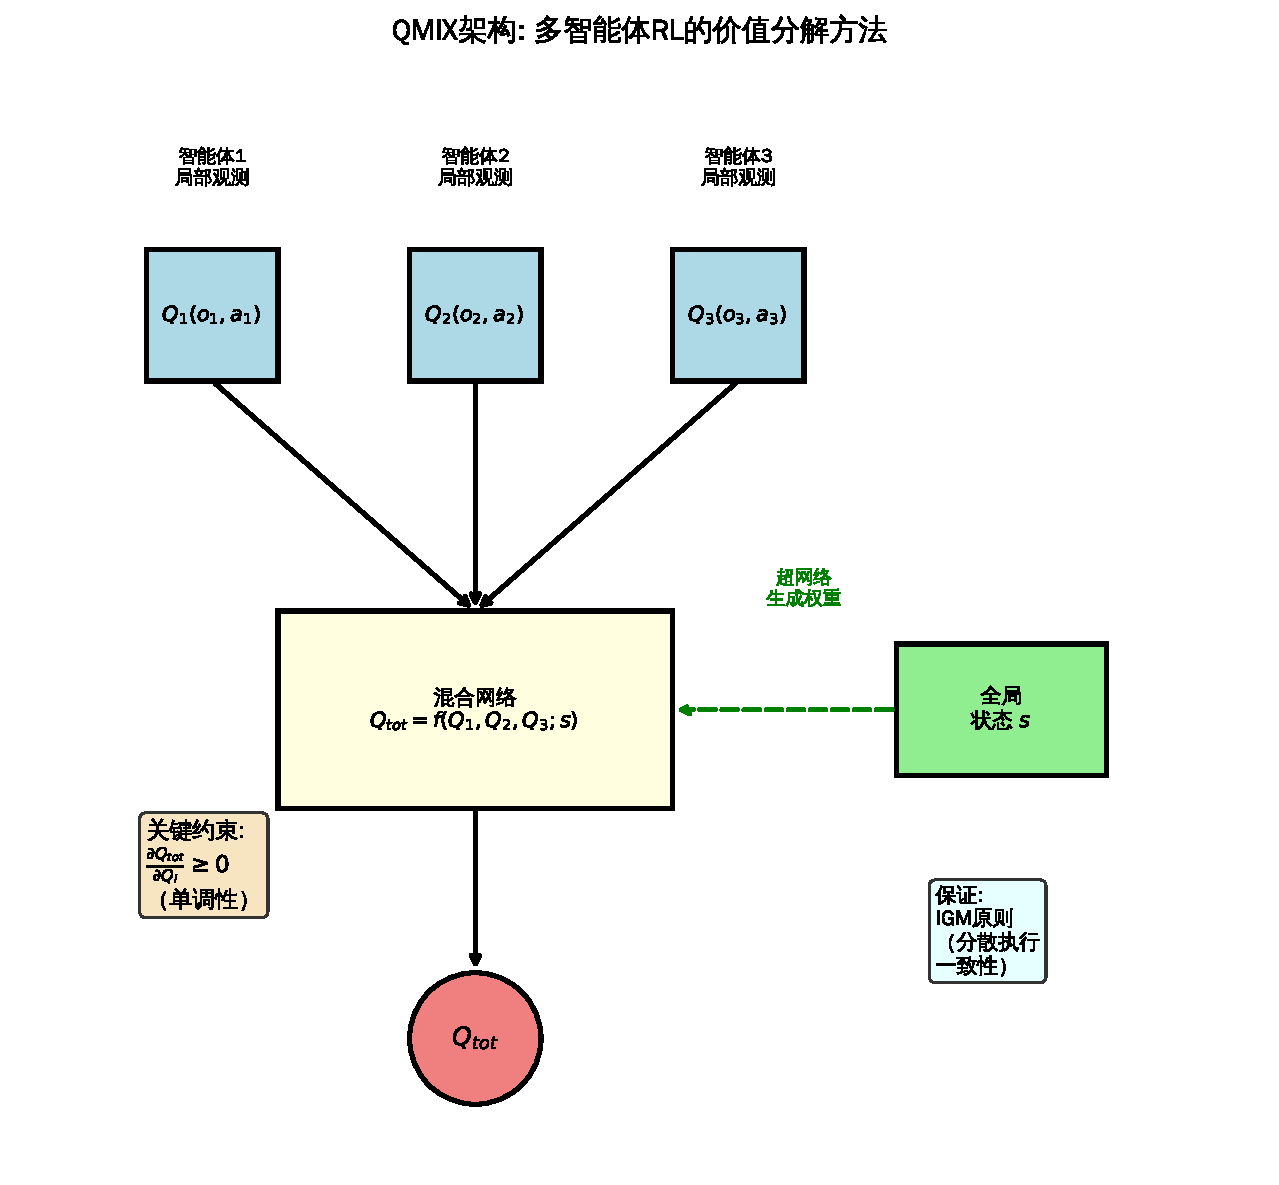
\includegraphics[width=0.8\textwidth]{figs_chap15/qmix_architecture.pdf}
\caption{QMIX架构示意图。每个智能体有自己的Q网络$Q_i(o_i, a_i)$，只使用局部观测。混合网络将各个局部Q值组合成全局Q值$Q_{tot}$。关键：混合网络的权重由超网络（Hypernetwork）根据全局状态$s$生成，且保证对$Q_i$的偏导非负（单调性约束），从而满足IGM原则。}
\label{fig:qmix}
\end{figure}

\textbf{QMIX架构的关键组件}（见图\ref{fig:qmix}）：
\begin{enumerate}
    \item \textbf{局部Q网络}：每个智能体$i$有一个Q网络$Q_i(o_i, a_i)$，只使用自己的观测
    \item \textbf{混合网络}：将所有局部Q值组合成全局Q值
    \item \textbf{超网络}：根据全局状态$s$生成混合网络的权重
    \item \textbf{非负权重}：通过绝对值或指数函数保证权重非负，从而满足单调性
\end{enumerate}

\begin{algorithm}
\caption{QMIX训练流程（伪代码）}
\begin{algorithmic}[1]
\State \textbf{输入}: 经验回放池，学习率$\alpha$，目标网络更新率$\tau$
\For{每个训练步}
    \State 从回放池采样一批经验 $(o, a, r, o', s, s', done)$
    \State \Comment{$o$: 各智能体观测, $a$: 各智能体动作, $s$: 全局状态}

    \State \textbf{计算当前Q值}:
    \For{每个智能体 $i$}
        \State $Q_i \leftarrow Q_i(o_i, a_i; \theta_i)$ \Comment{局部Q网络}
    \EndFor
    \State $Q_{tot} \leftarrow \text{MixingNetwork}(Q_1, \ldots, Q_N; s)$ \Comment{混合得到全局Q}

    \State \textbf{计算目标Q值}:
    \For{每个智能体 $i$}
        \State $Q'_i \leftarrow \max_{a'_i} Q^{target}_i(o'_i, a'_i)$ \Comment{目标网络}
    \EndFor
    \State $Q'_{tot} \leftarrow \text{MixingNetwork}^{target}(Q'_1, \ldots, Q'_N; s')$
    \State $y \leftarrow r + \gamma (1 - done) \cdot Q'_{tot}$ \Comment{TD目标}

    \State \textbf{更新网络}:
    \State $\mathcal{L} \leftarrow (Q_{tot} - y)^2$ \Comment{TD损失}
    \State 梯度下降更新所有网络参数
    \State 软更新目标网络: $\theta^{target} \leftarrow \tau \theta + (1-\tau) \theta^{target}$
\EndFor
\end{algorithmic}
\end{algorithm}

\begin{physicalintuition}
QMIX的单调性约束有深刻的物理意义：

\textbf{总能量是子系统能量的非线性叠加}。

想象一个物理系统由$N$个子系统组成，每个子系统有能量$E_i$。如果：
\begin{equation}
    \frac{\partial E_{tot}}{\partial E_i} \geq 0
\end{equation}

这意味着：任何子系统能量的增加都会导致总能量增加。没有"负能量贡献"。

QMIX假设的是一个\textbf{协作博弈}：每个智能体的"贡献"都是正向的。这在很多团队任务中是合理的（如星际争霸的微操、机器人协作搬运等）。

但如果智能体之间存在竞争关系（零和或混合博弈），QMIX的表达能力就不足了——这时需要其他方法。
\end{physicalintuition}

\subsection{策略梯度方法：MAPPO}

MAPPO是将PPO（近端策略优化）扩展到多智能体设置的方法。

\begin{definition}[MAPPO]
MAPPO使用Actor-Critic架构：
\begin{itemize}
    \item \textbf{Actor}（分散）：每个智能体$i$有自己的策略网络$\pi_i(a_i | o_i)$，只依赖局部观测
    \item \textbf{Critic}（集中）：一个共享的价值网络$V(s)$，使用全局状态
\end{itemize}

\review{第10章}{$L^{\text{CLIP}}$ 的来历见第10章扩展阅读"PPO：用裁剪代替约束"——它是把信赖域约束 $\mathrm{KL}(\pi_\theta \| \pi_{\theta_{\rm old}}) \le \delta$ 的拉格朗日形式换成一个便宜的替代品。}
策略更新使用PPO的裁剪目标：
\begin{equation}
    L^{\text{CLIP}}_i = \E\left[ \min\left( r_t(\theta) \hat{A}_t, \text{clip}(r_t(\theta), 1-\epsilon, 1+\epsilon) \hat{A}_t \right) \right]
\end{equation}
其中：
\begin{itemize}
    \item $r_t(\theta) = \frac{\pi_\theta(a_t | o_t)}{\pi_{\theta_{\text{old}}}(a_t | o_t)}$：新旧策略的概率比
    \item $\hat{A}_t$：优势函数估计（这个动作比平均好多少）
    \item $\epsilon$：裁剪参数（通常取0.1-0.2）
\end{itemize}
\end{definition}

\begin{remark}[MAPPO vs QMIX]
\begin{center}
\begin{tabular}{l|cc}
\toprule
& \textbf{QMIX} & \textbf{MAPPO} \\
\midrule
方法类型 & 价值分解 & 策略梯度 \\
动作空间 & 离散为主 & 离散/连续都可 \\
训练稳定性 & 较稳定 & 需要仔细调参 \\
表达能力 & 受单调性限制 & 更灵活 \\
适用场景 & 纯协作博弈 & 更广泛 \\
\bottomrule
\end{tabular}
\end{center}
\end{remark}

% ====================================================================================
\section{宏观极限：平均场博弈}
% ====================================================================================

\subsection{维度灾难与平均场近似}

当智能体数量很大时（如$N = 10000$个无人机、百万级的交通参与者），直接处理$N$体博弈面临\textbf{维度灾难}：
\begin{itemize}
    \item 联合状态空间：$\mathcal{S}^N$
    \item 联合动作空间：$\mathcal{A}^N$
    \item 存储和计算指数增长
\end{itemize}

\textbf{平均场近似}的思想来自统计物理：

\begin{quote}
\textit{当粒子数量趋于无穷时，忽略具体个体，只关注群体的统计分布。}
\end{quote}

\marginnote{\textbf{平均场博弈创始人}：MFG由法国数学家Jean-Michel Lasry和Pierre-Louis Lions于2006年合作提出；几乎同时，Huang、Malhamé 和 Caines 在加拿大独立提出了同样的思想。Lions是1994年菲尔兹奖得主（数学界最高荣誉），专长非线性PDE。他在法兰西公学院的MFG课程推动了该领域的蓬勃发展。}

\begin{definition}[平均场博弈]
在\textbf{平均场博弈}（Mean Field Game, MFG）中：
\begin{itemize}
    \item 有无穷多个同质（相同）智能体
    \item 每个智能体与群体分布$m(x, t)$交互，而不是与具体个体交互
    \item 群体分布由所有智能体的策略决定
\end{itemize}

\textbf{核心简化}：把``与$N$个具体对手的博弈''替换为``与群体分布的博弈''。
\end{definition}

\begin{example}[平均场近似的直观理解]
想象你是一滴水在大海中。

\textbf{微观视角}：你要考虑周围每一滴水的位置和速度（几乎不可能）

\textbf{平均场视角}：你只需要知道周围水的"平均流动方向"（密度场和速度场）

类似地，在有大量智能体的博弈中：
\begin{itemize}
    \item 你不需要知道每个对手的具体策略
    \item 你只需要知道对手群体的"分布"——有多少比例在做什么
    \item 基于这个分布，你做出最优响应
    \item 当每个人都这样做时，形成一个自洽的均衡
\end{itemize}
\end{example}

\subsection{MFG的核心思想：两步不动点}

理解MFG最关键的是把它看成一个\textbf{两步迭代过程}，最终要找的是一个\textbf{不动点}：

\begin{keyidea}[MFG的不动点结构——给大二同学的直观解释]
想象你是无数智能体中的一个，你需要做两件事：

\textbf{第一步：猜测别人的行为}

你不知道每个具体对手会做什么，但你可以``猜''一个群体分布$m(x,t)$——表示``在时刻$t$，有多少比例的智能体在位置$x$附近''。

\textbf{第二步：基于猜测，优化自己}

假设群体分布就是$m$，那么你面临的是一个\textbf{单人最优控制问题}——环境（别人的分布）已经固定了，你只需要最小化自己的代价。解这个问题得到\textbf{最优策略}$\pi^*(m)$和对应的\textbf{价值函数}$u(x,t)$。

\textbf{第三步：验证猜测是否自洽}

如果每个智能体都用$\pi^*(m)$这个策略，那么所有人的运动会产生一个新的密度分布$m'$。问题来了：$m'$和你最初猜的$m$一样吗？

\textbf{不动点条件}：如果$m' = m$，说明你的猜测是自洽的——每个人基于这个分布做最优决策，而这些最优决策恰好产生了这个分布。这就是\textbf{纳什均衡}！

\begin{center}
\begin{tikzpicture}[>=stealth, scale=0.9]
    \node[draw, rounded corners, fill=blue!15, minimum width=3cm, minimum height=1.2cm, align=center] (m) at (0, 0) {群体分布\\$m(x,t)$};
    \node[draw, rounded corners, fill=orange!15, minimum width=3cm, minimum height=1.2cm, align=center] (u) at (6, 0) {最优策略/价值函数\\$u(x,t), \pi^*$};

    \draw[->, thick] (m.east) -- node[above, font=\small] {固定$m$，解最优控制} node[below, font=\small, gray] {(HJB方程)} (u.west);
    \draw[->, thick] (u.south) .. controls (6, -2) and (0, -2) .. node[below, font=\small] {按$\pi^*$行动，推导密度} node[above, font=\small, gray] {(FP方程)} (m.south);

    \node[font=\small, red] at (3, -2.8) {\textbf{不动点}：$m \xrightarrow{\text{HJB}} u \xrightarrow{\text{FP}} m$};
\end{tikzpicture}
\end{center}
\end{keyidea}

\subsection{MFG的数学方程}

上面的直觉对应两个偏微分方程：

\begin{keyformula}[title=平均场博弈方程组]
\textbf{1. HJB方程}（``给定$m$，求最优策略''）：
\begin{equation}
    -\frac{\partial u}{\partial t} - \nu \Delta u + H(x, \nabla u, m) = 0, \quad u(x, T) = g(x), \qquad H(x, p, m) = \max_v \left[ -p \cdot v - L(x, v, m) \right]
\end{equation}
这是一个\textbf{后向方程}：从终端条件$g(x)$出发，往回算每个时刻的最优代价$u(x,t)$；$\nu \Delta u$ 项来自智能体受到的布朗运动扰动。
\review{第8章}{$u(x, t)$ 就是第8章的值函数 / 协态：HJB 从终端条件倒着算，和伴随方程"从未来往回算影响"是同一件事。这里的新意只在于 $H$ 里多了一个群体分布 $m$。}

\textbf{2. FP方程}（``给定最优策略，算密度演化''）：
\begin{equation}
    \frac{\partial m}{\partial t} + \nabla \cdot (m \cdot v^*) - \nu \Delta m = 0, \quad m(x, 0) = m_0(x)
\end{equation}
这是一个\textbf{前向方程}：从初始分布$m_0(x)$出发，根据最优速度场$v^* = -\nabla_p H$往前推演密度如何变化。

\textbf{耦合与不动点}：
\begin{itemize}
    \item HJB需要$m$：你的最优策略取决于别人在哪里（拥挤效应等）
    \item FP需要$u$：密度演化取决于大家的最优运动方向
    \item \textbf{纳什均衡} = 同时满足两个方程的$(u^*, m^*)$
\end{itemize}
\end{keyformula}

\begin{remark}[物理直觉]
\begin{itemize}
    \item \textbf{HJB方程}：类似量子力学中的Schrödinger方程，描述``价值波''的演化
    \item \textbf{FP方程}：就是连续性方程/扩散方程，描述概率密度的输运
\end{itemize}
MFG是统计力学和最优控制的交叉——群体行为的``热力学''。
\end{remark}

\begin{example}[线性二次MFG——一个可以精确求解的例子]
为了让上面的抽象方程变得具体，我们考虑一个最简单的MFG问题：

\textbf{场景}：无穷多个智能体在一维空间$x \in \mathbb{R}$上运动，时间$t \in [0, T]$。

\textbf{每个智能体的目标}：最小化自己的代价
\begin{equation}
    J = \int_0^T \left[ \frac{1}{2}v^2 + \frac{\alpha}{2}(x - \bar{x})^2 \right] dt + \frac{1}{2}x(T)^2
\end{equation}
其中：
\begin{itemize}
    \item $\frac{1}{2}v^2$：控制代价——速度越大，``油费''越贵
    \item $\frac{\alpha}{2}(x - \bar{x})^2$：\textbf{跟随代价}——$\alpha > 0$ 时希望靠近群体平均位置$\bar{x} = \int x \, m(x,t) dx$（$\alpha < 0$ 则变成拥挤代价，越远越好）
    \item $\frac{1}{2}x(T)^2$：终端代价——最后希望靠近原点
\end{itemize}

\textbf{动力学}：每个智能体按$\dot{x} = v$运动，并受布朗运动扰动（扩散系数$\nu$）。

\textbf{初始条件}：所有智能体初始集中在原点附近，$m_0(x) \sim \mathcal{N}(0, \sigma_0^2)$。

这个问题的MFG方程可以用有限差分法数值求解：HJB 从 $T$ 往回算、FP 从 $0$ 往前算，交替迭代直到不动点。图\ref{fig:mfg}就是这样算出来的一个\textbf{真实数值解}——为了让``别人对我的价格''看得见，图中把跟随代价换成了\textbf{拥挤代价}：$F(x,m)=\frac{\alpha}{2}(x-x_{\rm target})^2+\kappa\, m(x,t)$（想去目标点 $x_{\rm target}=1$，但当地人越多越贵），群体从 $x\approx-1$ 出发，终端代价 $g(x)=\frac{\alpha}{2}(x-x_{\rm target})^2$，参数 $\alpha=3$、$\kappa=2$、$\nu=0.05$、$T=1.5$。
\end{example}

\begin{figure}[htbp]
\centering
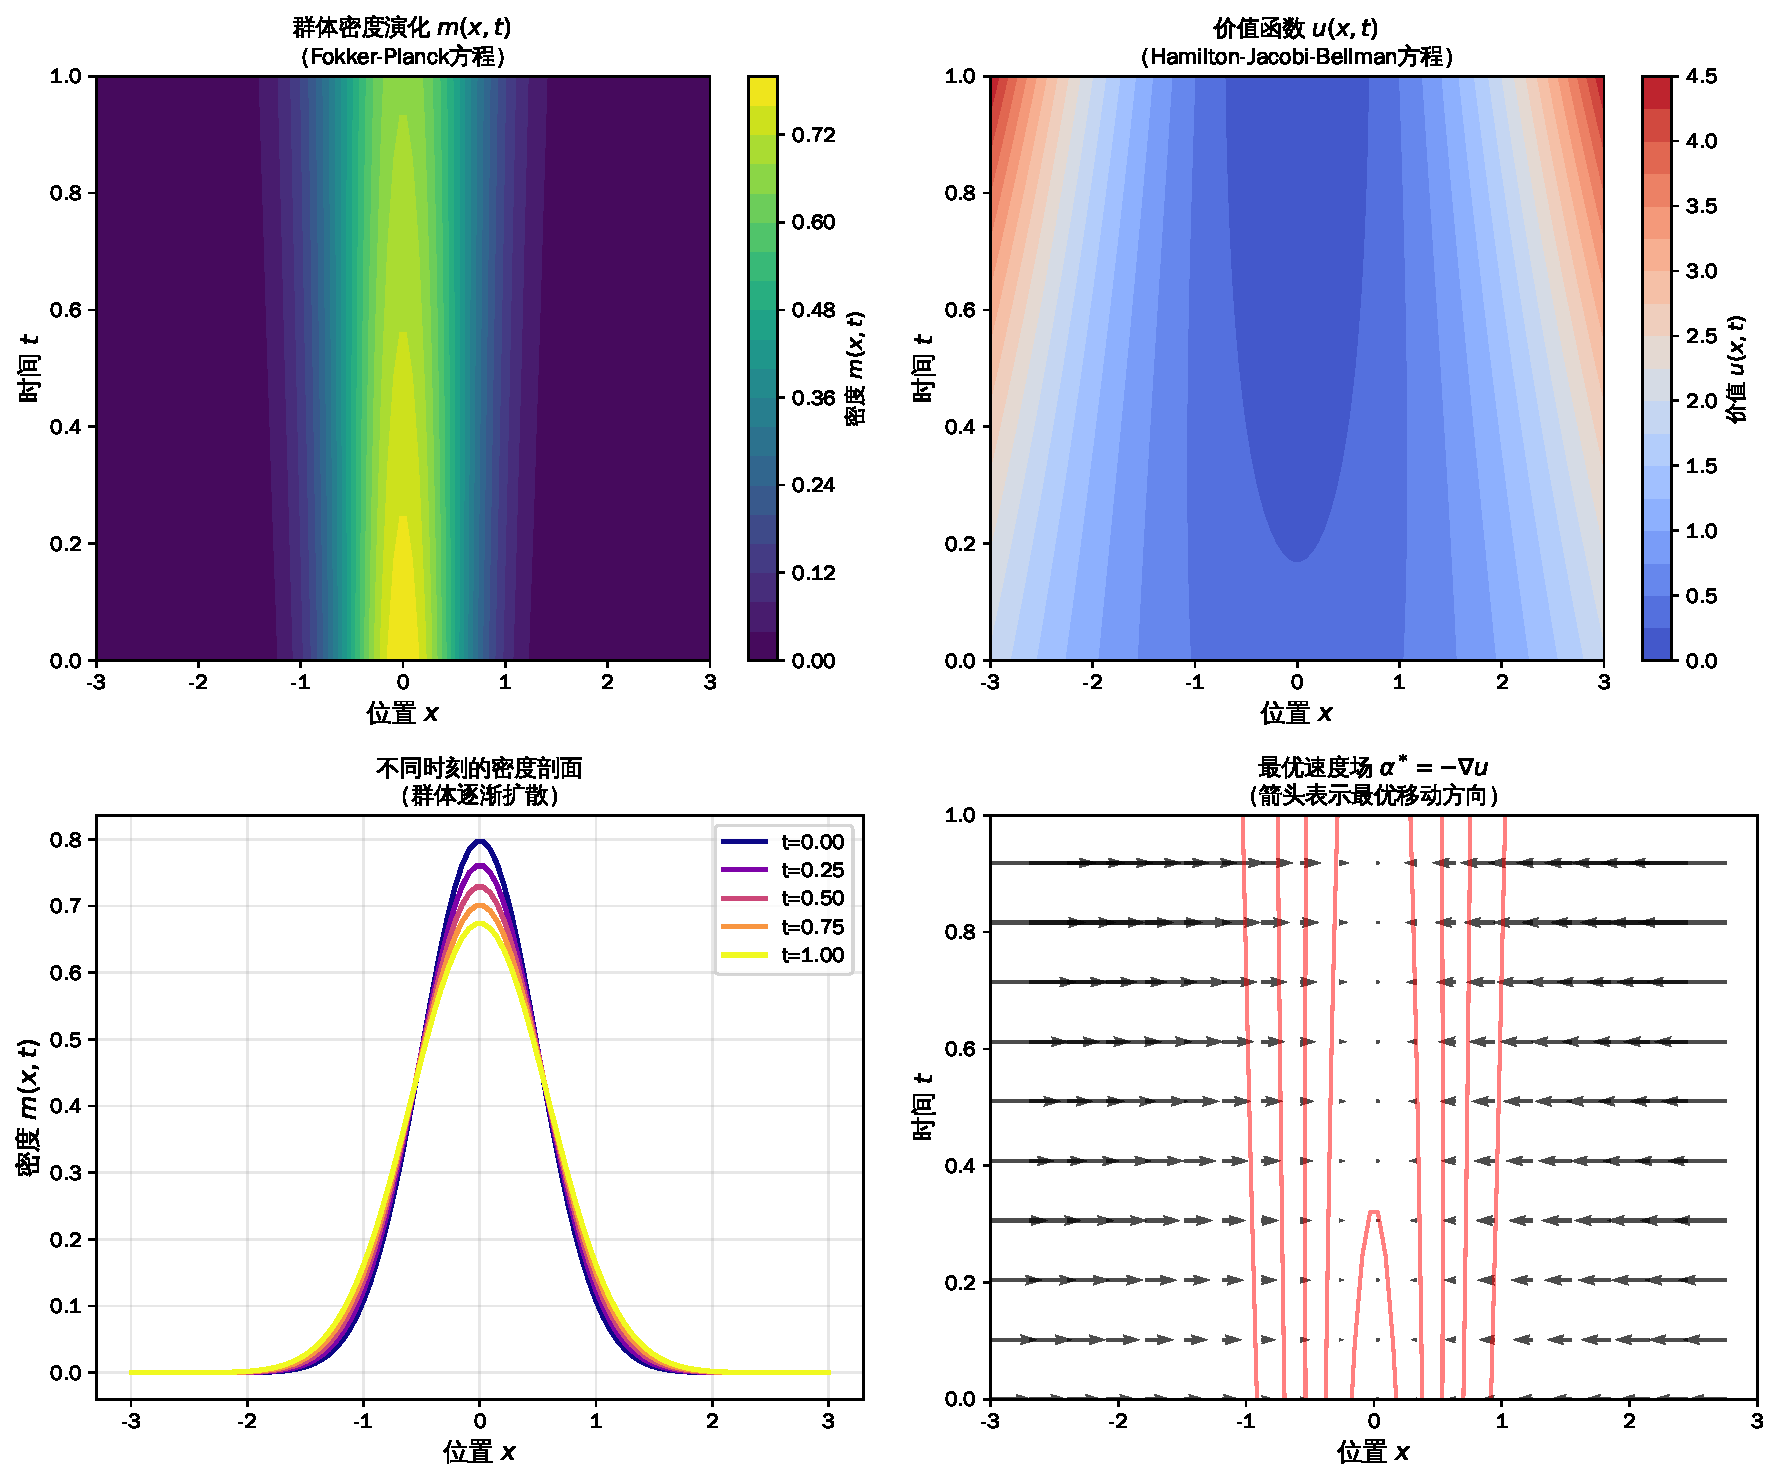
\includegraphics[width=0.95\textwidth]{figs_chap15/mfg_solution.pdf}
\caption{一维平均场博弈的数值解（有限差分 + 阻尼不动点迭代，代码 \texttt{code\_chap15/chap15\_mfg\_solver.py}）。每个人的运行代价是 $\frac12 v^2+\frac{\alpha}{2}(x-x_{\rm target})^2+\kappa\, m(x,t)$：想去目标点 $x_{\rm target}=1$（黑色点线），但讨厌拥挤。(a) 密度 $m(x,t)$：群体从 $x=-1$ 整体迁往目标点；红色虚线是沿最优速度场 $\dot x=-\partial_x u$ 积分出的个体轨迹——个体随群体一起走，但走在最前面的人会越过目标点，给后面的人让位。(b) 价值函数 $u(x,t)$（离目标越远代价越高）与最优速度 $v^*=-\partial_x u$（箭头）：$u$ 就是第8章的协态、本章的 $\lambda$，它的梯度直接告诉每个人该往哪走、走多快。(c) 不同时刻的密度剖面：有拥挤惩罚（$\kappa=2$）时，$t=T$ 的群体铺成峰值 $1.3$、标准差 $0.28$ 的宽平台；把 $\kappa$ 设为 $0$（灰色虚线）群体就挤成峰值 $2.6$、标准差 $0.16$ 的尖峰。(d) 不动点迭代残差：$m\to$HJB$\to u\to$FP$\to\tilde m$ 每一轮的变化量按指数衰减，约 110 轮后降到 $10^{-8}$——$(u^*,m^*)$ 确实是自洽的纳什均衡，不是画出来的。}
\label{fig:mfg}
\end{figure}

\textbf{从图中可以观察到}：
\begin{itemize}
    \item \textbf{(a)}：群体整体从 $x=-1$ 迁往目标点，但并不是每个人都停在目标点上——个体轨迹在 $t=T$ 时分散在 $x\approx0.5$ 到 $1.3$ 之间，前面的人越过目标点给后面的人让位。这就是拥挤代价 $\kappa m$ 在起作用：它是群体分布 $m$ 反过来施加给每个个体的``价格''
    \item \textbf{(b)}：价值函数在离目标远的地方最大（深色），越靠近目标越平缓；最优速度 $v^*=-\partial_x u$ 在目标点两侧相向指向目标，靠近目标后箭头变短——个体只按自己所在位置的 $\nabla u$ 行动，不需要知道别人的具体位置，这正是平均场近似的含义
    \item \textbf{(c)}：把 $\kappa$ 从 $2$ 调到 $0$，$t=T$ 的密度从宽平台变成尖峰。拥挤惩罚让个体宁可离目标远一点也要避开人群，宏观上就是群体``摊开''
    \item \textbf{(d)}：HJB 需要 $m$、FP 需要 $u$，两者互为约束；纳什均衡是这对方程组的不动点，残差按指数衰减到 $10^{-8}$ 说明它被真正算出来了（迭代时要加阻尼 $m\leftarrow(1-\theta)m+\theta\tilde m$，否则``人多的地方大家都想离开''会让迭代来回振荡）
\end{itemize}

% ====================================================================================
\section{本章小结}
% ====================================================================================

\begin{enumerate}
    \item \textbf{从优化到博弈}：单人优化只有一个决策者；多人博弈里每个人的最优依赖于他人的选择。纳什均衡是"没有人想单方面改变"的稳定状态。
    \item \textbf{静态博弈的分析工具}：广义纳什均衡 = 所有玩家的 KKT 条件同时成立；势博弈的自私行为恰好在优化一个全局势函数（保证收敛）；图博弈只有局部交互，可分布式计算；Braess 悖论说明增加选择反而可能让所有人更差。
    \item \textbf{动态博弈与深度 MARL}：CTDE 范式集中训练、分散执行；QMIX 用单调性约束保证 IGM；MAPPO 用集中式 Critic + 分散式 Actor。
    \item \textbf{宏观极限——平均场博弈}：$N \to \infty$ 时多体交互变成个体--场交互，HJB（后向）+ FP（前向）耦合方程组把博弈论接到了偏微分方程与统计物理。
\end{enumerate}

\begin{physicalmeaning}
\textbf{$\lambda$ 在本章的意义}：
\begin{itemize}
    \item \textbf{玩家自己的约束}：$\lambda_{ij}$ 是玩家 $i$ 为放松第 $j$ 条约束愿意付出的代价——第1章的影子价格原封不动，只是每人各有一份。
    \item \textbf{交通均衡}：需求约束的乘子 $\lambda_w = \partial \Phi^*/\partial d_w$ 等于均衡旅行时间；非负约束的乘子 $\mu_p$ 是路径 $p$ 比最短路"慢多少"。把 $t_a$ 换成边际社会成本后，多出来的 $x_a t_a'(x_a)$ 就是拥堵费。
    \item \textbf{平均场极限}：值函数 $u(x, t)$ 是 $\lambda$ 的连续版本（第8章的协态），$\nabla u$ 直接给出每个人的最优速度。
\end{itemize}
第4章 $\lambda$ = 约束力，第8章 $\lambda(t)$ = 伴随变量，第10章 $\lambda$ = 值函数梯度；本章它变成了"别人对我的价格"。下一章（第16章）它将以"安全约束的斥力"再次出现。
\end{physicalmeaning}

\begin{unification}[title=从微观到宏观的统一视角]
\begin{center}
\begin{tabular}{lccc}
\toprule
\textbf{维度} & \textbf{微观} & \textbf{中观} & \textbf{宏观} \\
\midrule
\textbf{智能体数} & 少量（2-10） & 中等（10-1000） & 无穷 \\
\textbf{核心对象} & 个体动作 $a_i$ & 联合动作 $\mathbf{a}$ & 密度分布 $m(x)$ \\
\textbf{静态模型} & 纳什均衡 & 图博弈/势博弈 & Wardrop均衡 \\
\textbf{动态模型} & 两人马尔可夫博弈 & Markov Game & MFG (HJB-FP) \\
\textbf{AI算法} & 自博弈（AlphaZero） & QMIX/MAPPO & Neural MFG \\
\textbf{物理类比} & 质点力学 & 多体系统 & 流体力学/统计物理 \\
\bottomrule
\end{tabular}
\end{center}

这个表格展示了一个美妙的对应：随着智能体数量的增加，我们从离散的个体视角逐渐过渡到连续的场视角，就像从牛顿力学过渡到流体力学一样。
\end{unification}

% ====================================================================================
\section{习题}
% ====================================================================================

\paragraph{计算题}
\begin{enumerate}
    \item \textbf{纳什均衡的理解}：
    考虑以下"协调博弈"：两个人要选择在哪里见面，可以选A地或B地。如果选同一个地方就能见面（代价0），选不同地方就见不到（代价1）。
    \begin{enumerate}
        \item 写出代价矩阵
        \item 找出所有纳什均衡
        \item 解释为什么会有多个纳什均衡
        \item 这个博弈是势博弈吗？为什么？
    \end{enumerate}
    
    \item \textbf{Braess悖论的变种}：
    在Braess悖论的例子中，如果免费道路AB的时间不是0，而是一个正数$c$，问：
    \begin{enumerate}
        \item $c$取什么范围时，悖论仍然存在（有免费道路更差）？
        \item $c$取什么值时，有道路和没道路的均衡时间相同？
        \item 给出直观解释。
    \end{enumerate}
    
    \item \textbf{图博弈的KKT条件}：
    对于代价函数$J_i = \frac{1}{2}(a_i - a_{i,0})^2 + \delta a_i \sum_{j \in N(i)} a_j$和约束$a_i \in [0, L]$：
    \begin{enumerate}
        \item 写出每个玩家的拉格朗日函数（提示：需要两个乘子，分别对应$a_i \geq 0$和$a_i \leq L$）
        \item 推导KKT条件
        \item 证明投影最优响应$a_i = \Pi_{[0,L]}(a_{i,0} - \delta \sum_{j} a_j)$满足KKT条件
        \item 其中$\Pi_{[0,L]}(x) = \max(0, \min(x, L))$是到区间$[0,L]$的投影
    \end{enumerate}
    
\end{enumerate}

\paragraph{证明题}
\begin{enumerate}
    \setcounter{enumi}{3}
    \item \textbf{QMIX的IGM证明}：
    证明：如果$\frac{\partial Q_{tot}}{\partial Q_i} \geq 0$对所有$i$成立，则IGM原则满足。
    
    提示：用反证法，假设存在$a'$使得$Q_{tot}(s, a') > Q_{tot}(s, a^*)$，其中$a_i^* = \arg\max Q_i$，推导矛盾。
    
\end{enumerate}

\paragraph{编程题}
\begin{enumerate}
    \setcounter{enumi}{4}
    \item \textbf{实现迭代最优响应}：
    对于例\ref{ex:lq_network}中的线性二次图博弈：
    \begin{enumerate}
        \item 用Python实现迭代最优响应算法
        \item 在一个10节点的随机图上测试收敛性
        \item 画出收敛曲线，验证线性收敛率
        \item 探索：$\delta$取什么值时算法不收敛？与图的谱半径有什么关系？
    \end{enumerate}
    
    \item \textbf{Braess悖论的数值验证}：
    参考本章的Python代码（\texttt{chap15\_generate\_figures.py}）：
    \begin{enumerate}
        \item 复现Braess悖论的计算
        \item 修改需求量（从4000变为其他值），观察悖论是否仍然存在
        \item 设计一个你自己的交通网络，尝试找到/构造Braess悖论
    \end{enumerate}
    
\end{enumerate}

\paragraph{思考题}
\begin{enumerate}
    \setcounter{enumi}{6}
    \item Wardrop 均衡的乘子 $\lambda_w$ 是均衡旅行时间。如果政府按边际社会成本 $x_a t_a'(x_a)$ 对每条路收拥堵费，新的均衡会变成什么？它和"系统最优"是什么关系？谁受益、谁受损？
    
    \item 第2章把拉格朗日函数看成 $x$ 与 $\lambda$ 的零和博弈。本章的势博弈是"$N$ 组 KKT 恰好是同一个函数的 KKT"。两者有什么共同点？一个非零和博弈什么时候会退化成单人优化？
\end{enumerate}

% ====================================================================================
\section*{扩展阅读：延伸文献}
\addcontentsline{toc}{section}{扩展阅读：延伸文献}
% ====================================================================================

\begin{enumerate}
    \item \textbf{博弈论入门}：Osborne, M. J. (2004). \textit{An Introduction to Game Theory}. Oxford University Press. 非常适合本科生的博弈论教材。

    \item \textbf{平均场博弈}：Lasry, J. M., \& Lions, P. L. (2007). Mean field games. \textit{Japanese Journal of Mathematics}, 2(1), 229-260. 平均场博弈的奠基性论文。

    \item \textbf{QMIX}：Rashid, T., et al. (2018). QMIX: Monotonic value function factorisation for deep multi-agent reinforcement learning. \textit{ICML 2018}. 价值分解方法的里程碑。

    \item \textbf{MAPPO}：Yu, C., et al. (2022). The surprising effectiveness of PPO in cooperative multi-agent games. \textit{NeurIPS 2022}. 展示了简单方法在多智能体RL中的强大能力。

    \item \textbf{Braess悖论}：Braess, D. (1968). Über ein Paradoxon aus der Verkehrsplanung. \textit{Unternehmensforschung}, 12(1), 258-268. 原始论文（德语）。

    \item \textbf{交通均衡}：Wardrop, J. G. (1952). Road paper. Some theoretical aspects of road traffic research. \textit{Proceedings of the Institution of Civil Engineers}, 1(3), 325-362. 交通均衡理论的经典。
\end{enumerate}
  % 第15章：多智能体与博弈
\chapter{物理世界模型：从约束优化到智能本质}

 

\vspace{1cm}

\begin{center}
\textit{"如果说拉格朗日力学描述了死物的运动规律，\\
那么我们如何用同样的数学语言描述智能体的思考与行动？"}
\end{center}

\vspace{1cm}

 

% ====================================================================================

\section*{引言：约束优化的终极问题}

% ====================================================================================

 

\marginnote{这一章是全书的Grand Finale。我们将看到，从牛顿力学到深度学习，从机器人控制到世界模型，所有这些看似不同的领域，都可以用同一个数学语言来统一：\textbf{约束优化}。}

 

让我们回顾这本书的旅程：

 

\begin{itemize}

    \item 第一章，我们从$F = ma$出发，看到拉格朗日如何用\textbf{约束优化}重新表述力学

    \item 中间的章节，我们学习了如何用神经网络求解PDE（PINN）、学习算子（神经算子）、处理多智能体博弈

    \item 现在，站在全书的终点，我们要问一个更深刻的问题：

\end{itemize}

 

\begin{quote}

\textbf{智能的本质是什么？}

\end{quote}

 

一块石头从山上滚下，遵循最小作用量原理——它"知道"如何找到最省能量的路径。但石头不是智能的。

 

一只猫追逐老鼠，也在某种意义上"优化"——但它的目标函数是什么？它的约束是什么？

 

一个自动驾驶系统在复杂的城市环境中导航，既要到达目的地（优化），又不能撞人（约束），还要预测其他车辆的行为（建模）。

 

\begin{framed}

\textbf{本章核心问题}：

 

如何用我们学过的数学工具——约束优化、动力系统、神经网络——来理解和构建\textbf{能够感知、预测、规划、行动}的智能系统？

 

\textbf{本章结构}：

\begin{enumerate}

    \item 什么是世界模型？——从"拟合数据"到"理解结构"

    \item 具身智能的数学本质——物理约束下的安全控制

    \item 可微物理——当牛顿定律变成计算图

    \item 终极猜想——自由能原理与智能的统一理论

\end{enumerate}

\end{framed}

 

% ====================================================================================

\section{什么是世界模型？}

% ====================================================================================

 

\subsection{从模型说起：什么是"理解"？}

 

在物理学中，"模型"是对现实世界的数学抽象。牛顿力学是一个模型，麦克斯韦方程是一个模型，薛定谔方程也是一个模型。

 

\begin{example}[你已经见过很多"模型"]

\begin{itemize}

    \item \textbf{单摆模型}：用角度$\theta$和角速度$\dot{\theta}$描述摆的状态

    \item \textbf{弹簧模型}：$F = -kx$，用位移描述弹力

    \item \textbf{热传导模型}：$\frac{\partial T}{\partial t} = \alpha \nabla^2 T$，用温度场描述热量流动

\end{itemize}

这些模型的共同点是：\textbf{用少数变量捕捉系统的本质行为}。

\end{example}

 

\begin{definition}[世界模型的直观定义]

在人工智能中，\textbf{世界模型}（World Model）是智能体对环境的内部表示。简单来说：

 

\begin{center}

\fbox{\textbf{世界模型 = 智能体脑中的"物理模拟器"}}

\end{center}

 

它回答一个核心问题：\textbf{如果我做了动作$a$，世界会变成什么样？}

\end{definition}

 

用数学语言表述：给定当前状态$s_t$和动作$a_t$，世界模型预测下一个状态$s_{t+1}$：

\begin{equation}
    \boxed{s_{t+1} = f(s_t, a_t) + \epsilon}
\end{equation}

其中：

\begin{itemize}

    \item $s_t$：\textbf{当前状态}——可以是机器人的位置、速度，也可以是游戏画面

    \item $a_t$：\textbf{动作}——智能体采取的行动，如"向左转"、"加速"

    \item $f$：\textbf{动力学函数}——描述状态如何演化的规则

    \item $\epsilon$：\textbf{不确定性}——世界并非完全可预测

\end{itemize}

 

\begin{example}[世界模型的生活实例]

想象你在打台球：

\begin{itemize}

    \item \textbf{状态}$s_t$：所有球的位置

    \item \textbf{动作}$a_t$：你击球的力度和角度

    \item \textbf{世界模型}$f$：预测击球后所有球会滚到哪里

\end{itemize}

 

一个台球高手脑中有一个精确的"物理模拟器"——他能在击球前"想象"出球的运动轨迹。这就是世界模型的本质！

\end{example}

 

\subsection{两种范式之争：像素vs本质}

 

当前AI领域对"世界模型"有两种截然不同的哲学。这场争论的核心是：\textbf{我们应该在什么空间中建模？}

 

\subsubsection{生成式世界模型（OpenAI/Sora路线）}

 

\marginnote{Sora是OpenAI在2024年发布的视频生成模型，能够生成高度逼真的视频。它被一些人认为是"物理模拟器"，因为它似乎"理解"了物体如何运动。}

 

核心思想：\textbf{预测原始像素}。

 

如果一个模型能够准确预测视频的下一帧，那么它一定"理解"了物理规律——因为没有理解物理，就无法预测物体会怎么运动。

 

数学表述：学习条件概率分布

\begin{equation}
    P(x_{t+1} | x_1, x_2, \ldots, x_t)
\end{equation}

其中$x_t$是第$t$帧的像素（比如一张$256 \times 256$的图片有65536个像素值）。

 

\begin{example}[视频预测作为物理模拟]

想象一个视频：一个球从桌子边缘滚落。

 

要准确预测下一帧，模型需要"知道"：

\begin{itemize}

    \item 重力会让球加速下落（$a = g \approx 9.8 \text{m/s}^2$）

    \item 球是圆的，所以会滚动而不是滑动

    \item 空气阻力可以忽略（对于慢速运动）

    \item 球落地后会弹起（如果是弹性球）

\end{itemize}

 

如果模型能预测这些，是不是意味着它"学会"了物理？

\end{example}

 

\subsubsection{联合嵌入预测架构（LeCun/JEPA路线）}

 

\marginnote{\textbf{Yann LeCun}(1960--)：2018年图灵奖得主（与Hinton、Bengio共获），卷积神经网络之父，现任Meta首席AI科学家。他在1990年代开发的LeNet是现代CNN的鼻祖。近年他大力推动``世界模型''研究方向，批评纯语言模型是``通往AGI的错误道路''。}

 

Yann LeCun对生成式路线的批评是尖锐的：

 

\begin{quote}

\textit{"预测像素是在浪费算力去拟合随机噪声。风吹动树叶的每一个细节是不可预测的，但这不重要！重要的是树在那里，风在吹。"}

\end{quote}

 

核心思想：\textbf{在抽象特征空间预测，而不是在像素空间}。

 

\begin{definition}[JEPA架构——用大白话解释]

\textbf{联合嵌入预测架构}（Joint-Embedding Predictive Architecture，JEPA）的思想是：

\begin{enumerate}

    \item \textbf{先压缩}：把高维的像素压缩成低维的"本质特征"

    \item \textbf{再预测}：在特征空间做预测（而不是在像素空间）

    \item \textbf{比较特征}：预测的特征和真实的特征应该接近

\end{enumerate}

\end{definition}

 

用数学语言：

\begin{itemize}

    \item \textbf{编码器}$E$：将观测$x$（如图片）映射到抽象表征$s = E(x)$

    \item \textbf{预测器}$P$：在表征空间预测$\hat{s}_{t+1} = P(s_t, a_t)$

    \item \textbf{距离函数}$D$：衡量预测与真实表征的距离$D(\hat{s}_{t+1}, s_{t+1})$

\end{itemize}

 

\begin{figure}[htbp]

\centering

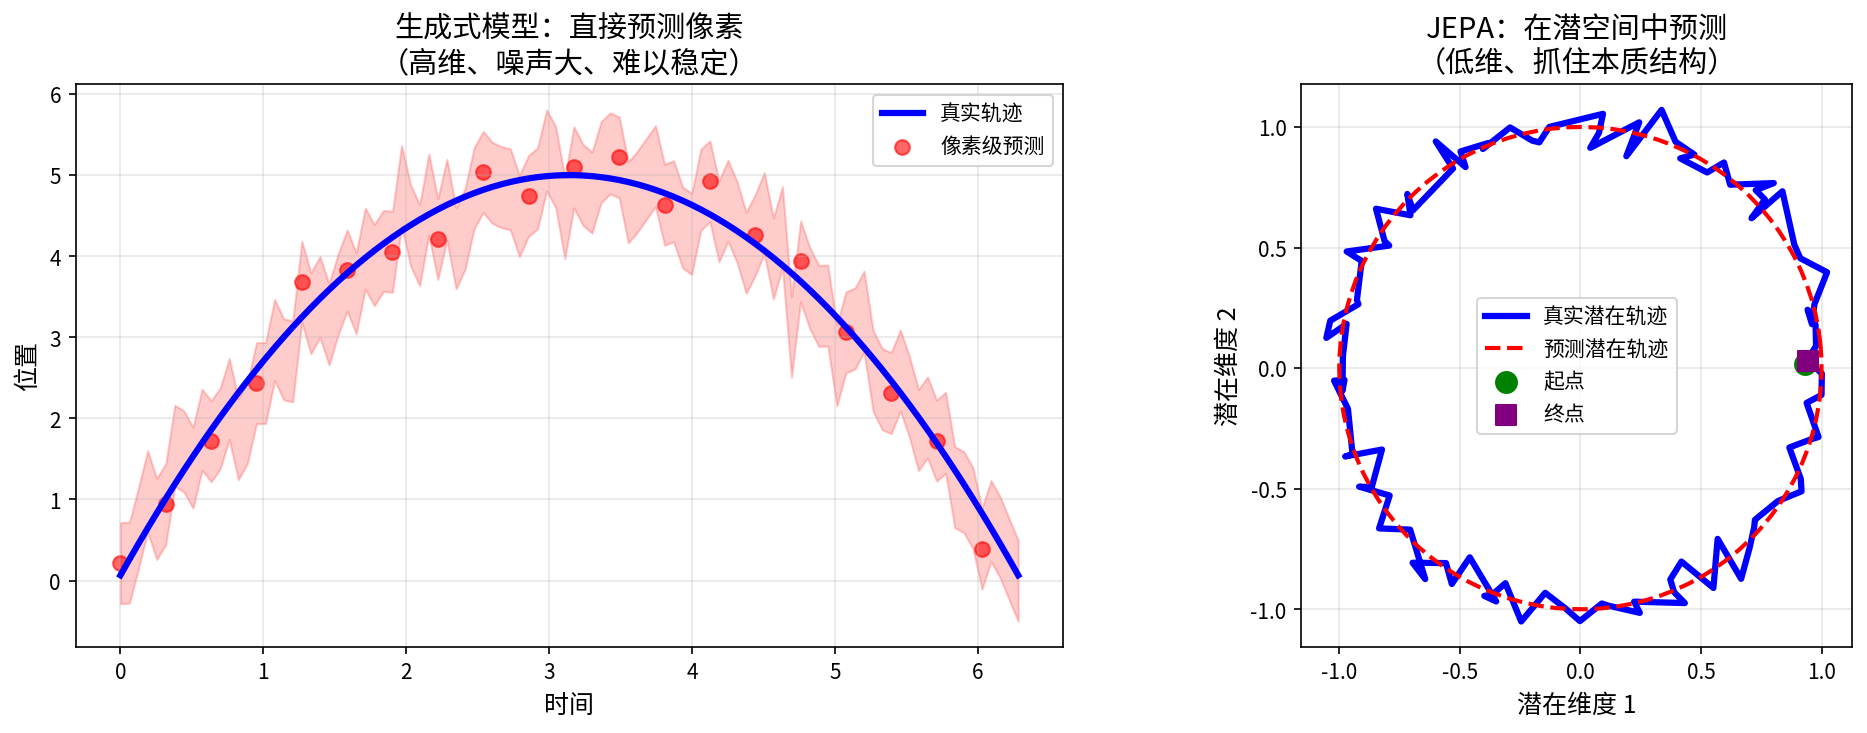
\includegraphics[width=0.95\textwidth]{figs_chap16/paradigm_comparison.png}

\caption{两种世界模型范式对比。左图：生成式模型直接预测像素，预测结果有噪声；右图：JEPA在低维潜空间预测，轨迹更加平滑、本质。}

\label{fig:paradigm_comparison}

\end{figure}

 

\begin{keyinsight}

\textbf{两种范式的约束优化视角}：

 

\textbf{生成式模型}：试图拟合整个数据分布$P(x)$

\begin{equation}
    \min_\theta \E_{x \sim \text{data}}[-\log P_\theta(x)]
\end{equation}

这是一个\textbf{无约束}的密度估计问题——要建模所有细节。

 

\textbf{JEPA}：学习表征空间中的\textbf{约束关系}

\begin{equation}
    \min_{E, P} \E[D(P(E(x_t), a_t), E(x_{t+1}))] \quad \text{s.t. 表征不能坍缩为常数}
\end{equation}

这是一个\textbf{有约束}的流形学习问题——只学习本质特征。

\end{keyinsight}

 

\begin{example}[类比：记忆 vs 理解]

想象两个学生准备考试：

\begin{itemize}

    \item \textbf{学生A}（生成式）：把课本逐字背下来，包括每个标点符号

    \item \textbf{学生B}（JEPA）：理解核心概念，用自己的话总结

\end{itemize}

学生A的"模型"可以完美复述课本，但占用大量记忆。学生B的"模型"更紧凑，而且能举一反三。

 

JEPA的哲学就是：\textbf{学习本质，忽略细节}。

\end{example}

 

\subsection{潜空间动力学：在梦境中学习}

 

无论选择哪种范式，一个共同的思想是：在\textbf{潜空间}（latent space）中建模动力学。

 

\begin{definition}[潜空间——什么是"潜"？]

"潜空间"这个名字来自"潜在变量"（latent variable）——它是隐藏在数据背后、我们无法直接观测的变量。

 

\textbf{类比}：你看到一个人在笑（观测），但你看不到他的心情（潜变量）。心情是"潜在"的，但它决定了外在表现。

\end{definition}

 

\begin{definition}[潜空间动力学模型的三个组件]

一个完整的潜空间动力学模型包含三个部分：

\begin{align}
    z_t &= \text{Encoder}(o_t) \quad \text{（\textbf{感知}：把观测压缩成潜态）} \\
    z_{t+1} &= \text{Dynamics}(z_t, a_t) \quad \text{（\textbf{预测}：潜态如何演化）} \\
    \hat{o}_{t+1} &= \text{Decoder}(z_{t+1}) \quad \text{（\textbf{想象}：从潜态还原观测）}
\end{align}

 

其中：

\begin{itemize}

    \item $o_t$：\textbf{观测}（observation），如摄像头拍到的图像，维度很高

    \item $z_t$：\textbf{潜态}（latent state），压缩后的表示，维度很低

    \item $a_t$：\textbf{动作}（action），智能体的行为

\end{itemize}

\end{definition}

 

\begin{figure}[htbp]

\centering

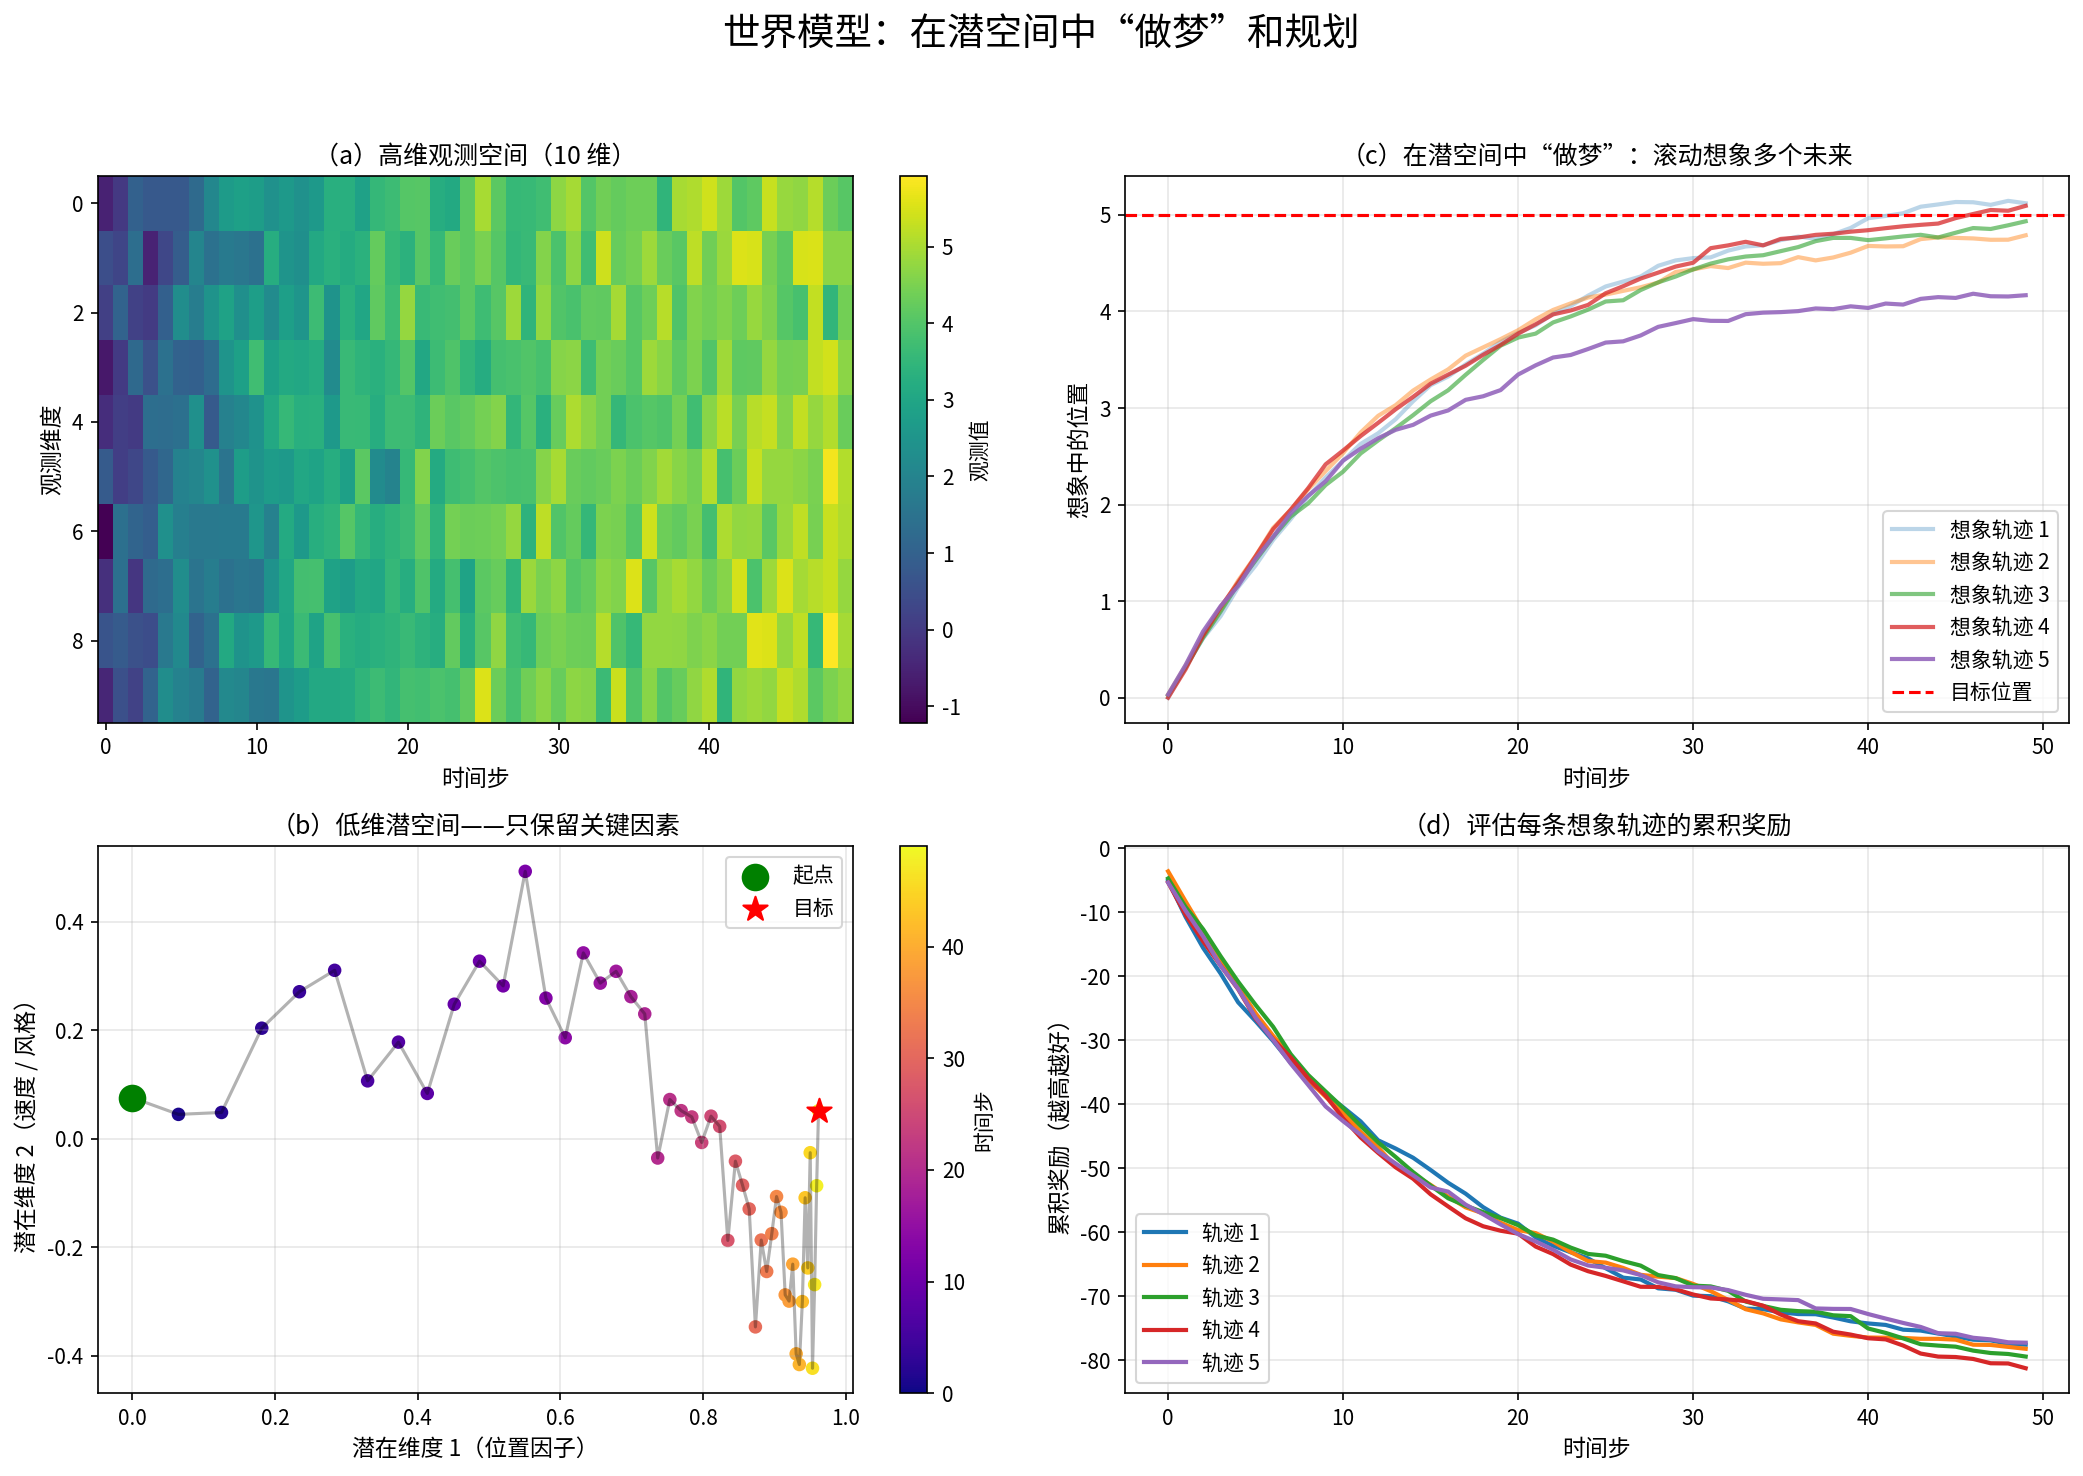
\includegraphics[width=0.95\textwidth]{figs_chap16/latent_dynamics.png}

\caption{潜空间动力学模型示意图。(a)高维观测数据难以直接处理；(b)编码器将其压缩到2维潜空间，清晰显示状态演化；(c)在潜空间中可以"做梦"——想象多条可能的未来轨迹；(d)评估每条轨迹的累积奖励，选择最优动作。}

\label{fig:latent_dynamics}

\end{figure}

 

\begin{example}[Dreamer算法：在梦中学习]

\marginnote{Dreamer是DeepMind提出的世界模型强化学习方法。它的核心思想是：在潜空间中"做梦"，想象可能的未来，然后在想象中学习策略。}

 

Dreamer算法的工作流程就像人类做白日梦：

 

\textbf{第一步：学习世界模型}

\begin{itemize}

    \item 收集真实环境中的经验$(o_1, a_1, r_1, o_2, \ldots)$

    \item 训练编码器、动力学模型、解码器

\end{itemize}

 

\textbf{第二步：在想象中规划}

\begin{itemize}

    \item 从当前潜态$z_t$出发

    \item 在潜空间中"展开"未来：$z_{t+1} = f(z_t, a_t)$

    \item 预测每一步的奖励：$\hat{r}_t = R(z_t)$

    \item 尝试不同的动作序列，找到累积奖励最高的那个

\end{itemize}

 

\textbf{第三步：执行并学习}

\begin{itemize}

    \item 执行规划得到的动作

    \item 用新数据更新世界模型

\end{itemize}

 

这就像你在脑中"预演"打台球——你想象不同的击球方式，预测结果，选择最好的那个，然后才真正动手。

\end{example}

 

\begin{physicalintuition}

\textbf{潜空间与广义坐标的深刻联系}

 

回想拉格朗日力学：我们用\textbf{广义坐标}$q$来描述系统状态，而不是用笛卡尔坐标。广义坐标的选择应该"尊重约束"——比如用角度$\theta$描述单摆，而不是用$(x, y)$坐标。

 

潜空间就是神经网络学到的"广义坐标"！它应该：

\begin{itemize}

    \item 捕捉系统的本质自由度（单摆只有1个自由度）

    \item 忽略无关的细节（如光照变化、背景噪声）

    \item 使动力学方程尽可能简单

\end{itemize}

 

\textbf{好的潜空间 = 好的广义坐标 = 对称性和约束的正确表达}

\end{physicalintuition}

 

下面是潜空间动力学模型的伪代码，帮助理解其核心结构：

 

\begin{algorithm}[H]
\caption{潜空间世界模型的核心流程}
\begin{algorithmic}[1]
\Require 观测序列 $\{o_1, o_2, \ldots, o_T\}$，动作序列 $\{a_1, a_2, \ldots, a_{T-1}\}$
\State \textbf{// 第一步：编码——将高维观测压缩到低维潜空间}
\For{$t = 1$ to $T$}
    \State $z_t \gets \text{Encoder}(o_t)$ \Comment{例如：$256\times256$图像 $\to$ 64维向量}
\EndFor
\State \textbf{// 第二步：学习动力学——潜态如何随动作演化}
\For{$t = 1$ to $T-1$}
    \State $\hat{z}_{t+1} \gets \text{Dynamics}(z_t, a_t)$ \Comment{预测下一个潜态}
    \State $\text{loss} \gets \text{loss} + \|z_{t+1} - \hat{z}_{t+1}\|^2$ \Comment{预测误差}
\EndFor
\State \textbf{// 第三步：想象未来——在潜空间中"做梦"}
\State $z_{\text{current}} \gets \text{Encoder}(o_{\text{current}})$
\For{每个候选动作序列 $\{a_1, a_2, \ldots, a_H\}$}
    \State $z \gets z_{\text{current}}$
    \State $\text{total\_reward} \gets 0$
    \For{$h = 1$ to $H$}
        \State $z \gets \text{Dynamics}(z, a_h)$
        \State $\text{total\_reward} \gets \text{total\_reward} + \text{RewardPredictor}(z)$
    \EndFor
    \State 记录该动作序列的总奖励
\EndFor
\State \textbf{return} 总奖励最高的动作序列的第一个动作
\end{algorithmic}
\end{algorithm}

 

% ====================================================================================

\section{具身智能的数学本质：安全约束下的控制}

% ====================================================================================

 

世界模型告诉我们"世界会怎么变"。但对于\textbf{具身智能}（Embodied Intelligence）——机器人、自动驾驶、无人机——光有预测还不够。

 

我们还需要回答：\textbf{如何在物理约束下安全地行动？}

 

\subsection{约束的本质变了}

 

回顾我们在第一章学过的拉格朗日力学。当时的约束是这样的：

\begin{equation}
    \mathcal{L} = T - V + \lambda g(q)
\end{equation}

 

这里的约束$g(q) = 0$是\textbf{等式约束}——比如单摆必须沿圆弧运动，系统没有选择。

 

但在机器人控制中，约束变成了\textbf{不等式约束}——有一片"禁区"，系统不能进入：

\begin{itemize}

    \item \textbf{安全边界}：$\text{距离障碍物}(x) \geq d_{\min}$（不能撞墙）

    \item \textbf{关节限位}：$q_{\min} \leq q \leq q_{\max}$（机械臂不能弯曲超过极限）

    \item \textbf{摩擦锥}：$\|f_{\text{切向}}\| \leq \mu f_{\text{法向}}$（脚不能打滑）

    \item \textbf{能量约束}：$\|u\|^2 \leq u_{\max}^2$（电机功率有限）

\end{itemize}

 

\begin{example}[等式约束 vs 不等式约束]

\begin{itemize}

    \item \textbf{等式约束}：火车必须在轨道上（没得选）

    \item \textbf{不等式约束}：汽车不能开到悬崖下面（有一片禁区，但路很宽）

\end{itemize}

\end{example}

 

\subsection{控制障碍函数：安全的数学保证}

 

如何保证机器人"永远不会撞墙"？这听起来是一个很强的要求——我们需要一个数学工具来提供\textbf{安全保证}。

 

\begin{definition}[安全集合与障碍函数——用通俗语言解释]

想象你在一个房间里，房间中央有一根柱子（障碍物）。我们定义一个函数$h(x)$：

 

\begin{equation}
    h(x) = \text{（你离柱子的距离）} - \text{（安全距离）}
\end{equation}

 

这个函数告诉我们：

\begin{itemize}

    \item $h(x) > 0$：你离柱子足够远，\textbf{安全}

    \item $h(x) = 0$：你刚好在安全边界上，\textbf{临界}

    \item $h(x) < 0$：你离柱子太近了，\textbf{危险}！

\end{itemize}

 

\textbf{安全集合}就是所有$h(x) \geq 0$的点构成的区域。

\end{definition}

 

更具体地，对于一个位于$x_{\text{obs}}$的圆形障碍物，安全距离为$d$，障碍函数可以定义为：

\begin{equation}
    h(x) = \|x - x_{\text{obs}}\|^2 - d^2
\end{equation}

 

这里$\|x - x_{\text{obs}}\|$是你到障碍物中心的距离。

 

\begin{theorem}[控制障碍函数条件——如何保证安全？]

\label{thm:cbf}

考虑一个受控系统：

\begin{equation}
    \dot{x} = f(x) + g(x)u
\end{equation}

其中$x$是状态，$u$是控制输入，$f(x)$是系统的自然演化，$g(x)$描述控制如何影响系统。

 

\textbf{关键问题}：我们想让$h(x)$永远保持非负（永远安全）。根据微积分，$h$的变化率是：

\begin{equation}
    \dot{h} = \frac{\partial h}{\partial x} \cdot \dot{x} = \frac{\partial h}{\partial x} \cdot (f(x) + g(x)u)
\end{equation}

 

\textbf{核心条件}：如果我们能保证

\begin{equation}
    \boxed{\dot{h}(x, u) \geq -\alpha \cdot h(x)}
\end{equation}

其中$\alpha > 0$是一个正常数，那么安全集合$h(x) \geq 0$是\textbf{前向不变}的——一旦进入安全区域，永远不会离开。

\end{theorem}

 

\begin{physicalintuition}

\textbf{为什么这个条件能保证安全？}

 

条件$\dot{h} \geq -\alpha h$的含义是：

\begin{itemize}

    \item 当$h$很大时（离危险很远），$\dot{h}$可以是负的——允许靠近

    \item 当$h$接近0时（快到边界了），$\dot{h}$必须接近0或为正——不能再靠近

    \item 当$h = 0$时（恰好在边界上），$\dot{h} \geq 0$——只能离开，不能进入危险区

\end{itemize}

 

这就像一个"软弹簧"把你推离危险区域——越靠近边界，推力越大。

\end{physicalintuition}

 

\begin{keyformula}[title=基于CBF的安全控制器]

假设我们有一个\textbf{标称控制器}$u_{\text{ref}}(x)$——这是我们"想要"的控制（比如"直线走向目标"）。

 

问题是：$u_{\text{ref}}$可能会导致碰撞。我们需要找一个\textbf{尽量接近}$u_{\text{ref}}$但\textbf{保证安全}的控制$u^*$。

 

这是一个\textbf{二次规划}（QP）问题：

\begin{equation}
    u^*(x) = \arg\min_{u} \frac{1}{2}\|u - u_{\text{ref}}(x)\|^2
\end{equation}

\begin{equation}
    \text{约束条件：} \quad \underbrace{\frac{\partial h}{\partial x}f(x)}_{\text{自然漂移}} + \underbrace{\frac{\partial h}{\partial x}g(x) \cdot u}_{\text{控制效果}} + \alpha h(x) \geq 0
\end{equation}

 

\textbf{直观解释}：在所有满足安全约束的控制中，选择和原计划最接近的那个。

\end{keyformula}

 

好消息是，这个QP有\textbf{闭式解}！利用拉格朗日乘子法（KKT条件）：

\begin{equation}
    u^* = u_{\text{ref}} - \lambda^* \left(\frac{\partial h}{\partial x}g(x)\right)^T
\end{equation}

其中$\lambda^* \geq 0$是拉格朗日乘子，只在约束激活（接近危险）时非零。

 

\begin{physicalintuition}

\textbf{CBF与拉格朗日力学的深刻联系}

 

这里的$\lambda^*$和拉格朗日力学中的约束力$\lambda$有着相同的物理意义！

 

\textbf{拉格朗日力学}：

\begin{itemize}

    \item 约束力$\lambda$维持等式约束$g(q) = 0$

    \item $\lambda$垂直于约束面，阻止系统"穿出"

\end{itemize}

 

\textbf{CBF控制}：

\begin{itemize}

    \item 安全修正项$\lambda^* (\nabla h \cdot g)^T$维持不等式约束$h(x) \geq 0$

    \item $\lambda^*$只在接近边界时激活，产生"斥力"

\end{itemize}

 

\textbf{统一视角}：两者都是\textbf{约束优化}——拉格朗日乘子是"违反约束的代价"。

\end{physicalintuition}

 

\subsection{实验结果：CBF控制器的效果}

 

下面我们通过一个简单的实验来展示CBF控制器的效果。场景设置：

\begin{itemize}

    \item 起点：$(0, 0)$

    \item 目标：$(10, 10)$

    \item 障碍物：位于$(5, 5)$，安全距离$d = 1.5$

    \item 标称控制器：直接朝目标方向走

\end{itemize}

 

\begin{figure}[htbp]

\centering

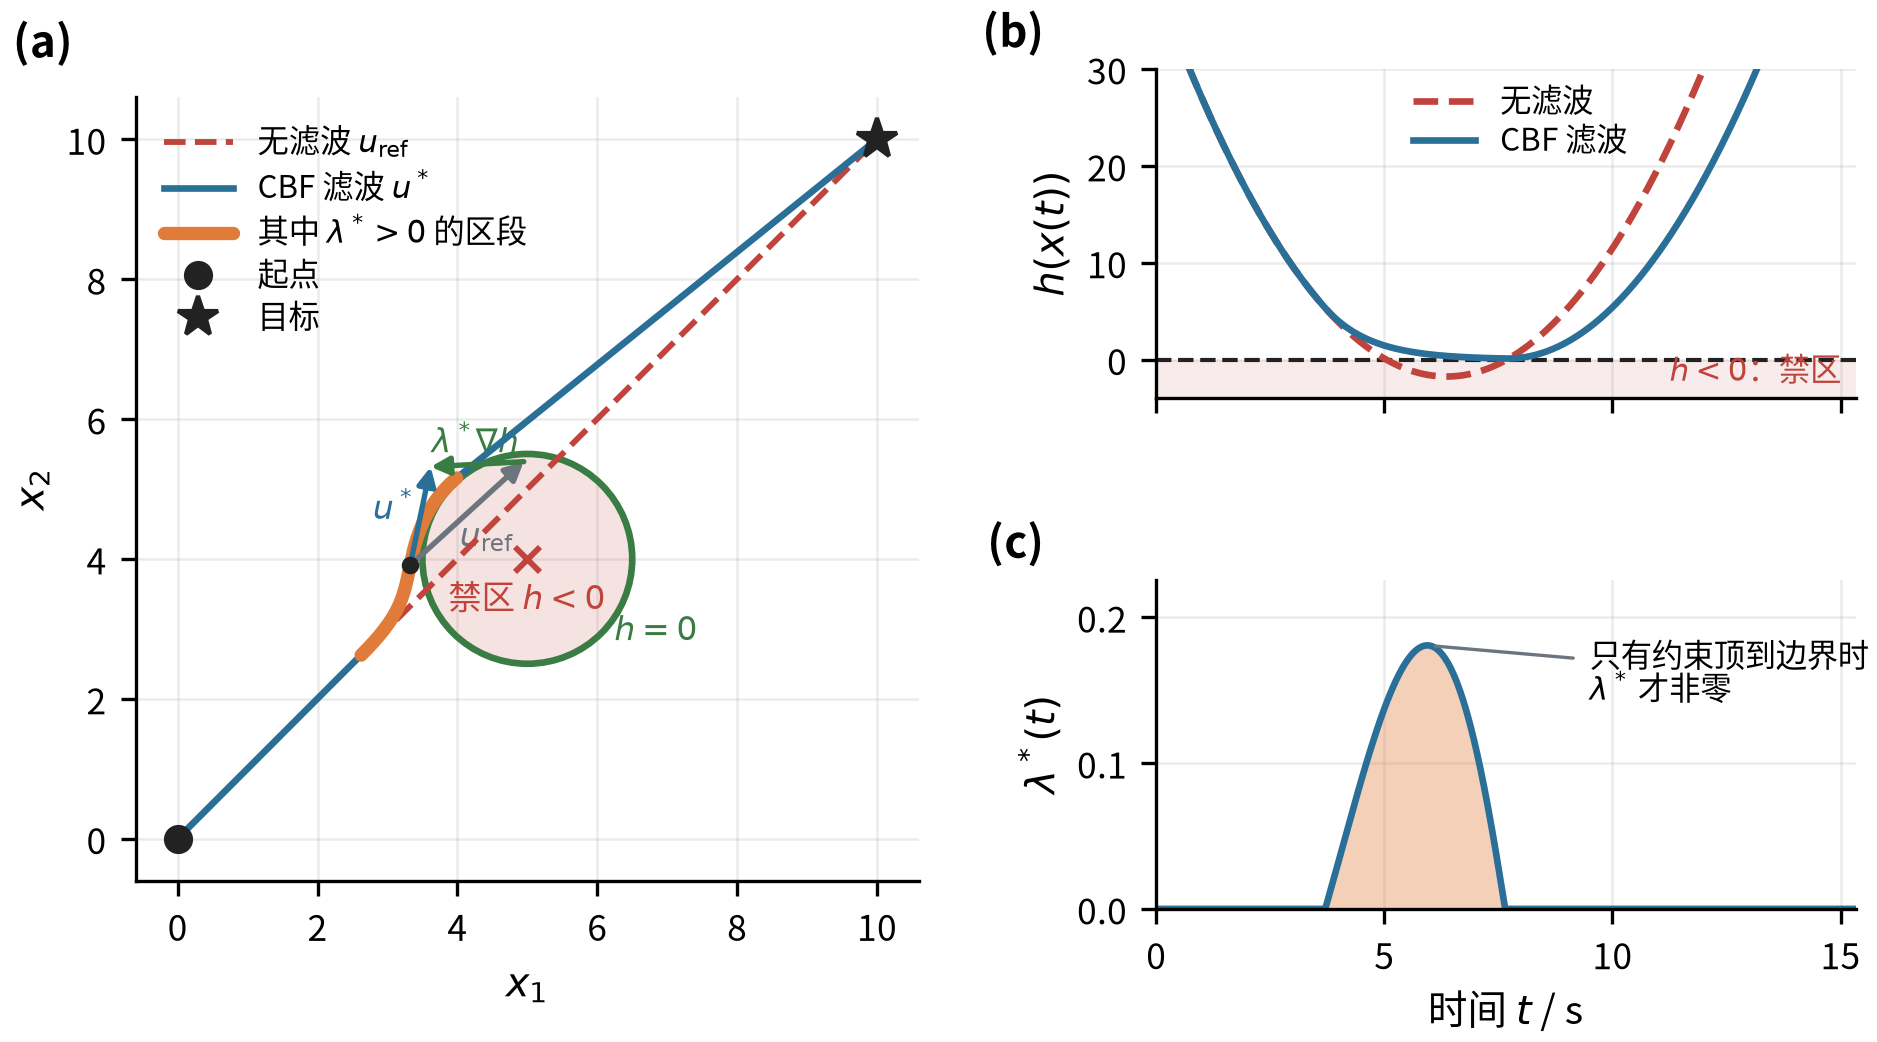
\includegraphics[width=0.95\textwidth]{figs_chap16/cbf_controller.png}

\caption{CBF安全控制器实验结果。(a)无CBF时，智能体直线冲向目标，穿过障碍物！(b)有CBF时，智能体绕开障碍物安全到达目标。(c)障碍函数$h(x)$随时间变化：无CBF时$h$变负（进入危险区），有CBF时$h$始终非负。(d)控制输入对比：CBF只在必要时（接近障碍物时）修正控制。}

\label{fig:cbf_controller}

\end{figure}

 

\textbf{关键观察}：

\begin{enumerate}

    \item \textbf{安全保证}：有CBF时，障碍函数$h(x)$始终保持非负，系统永远不会进入危险区域。

    \item \textbf{最小干预}：CBF控制器是"懒惰"的——只有当系统接近危险边界时才会干预。在远离障碍物的地方，$u_{\text{safe}} \approx u_{\text{ref}}$。

    \item \textbf{光滑绕行}：系统自然地绕开障碍物，轨迹平滑，没有突变。

\end{enumerate}

 

\begin{figure}[htbp]

\centering

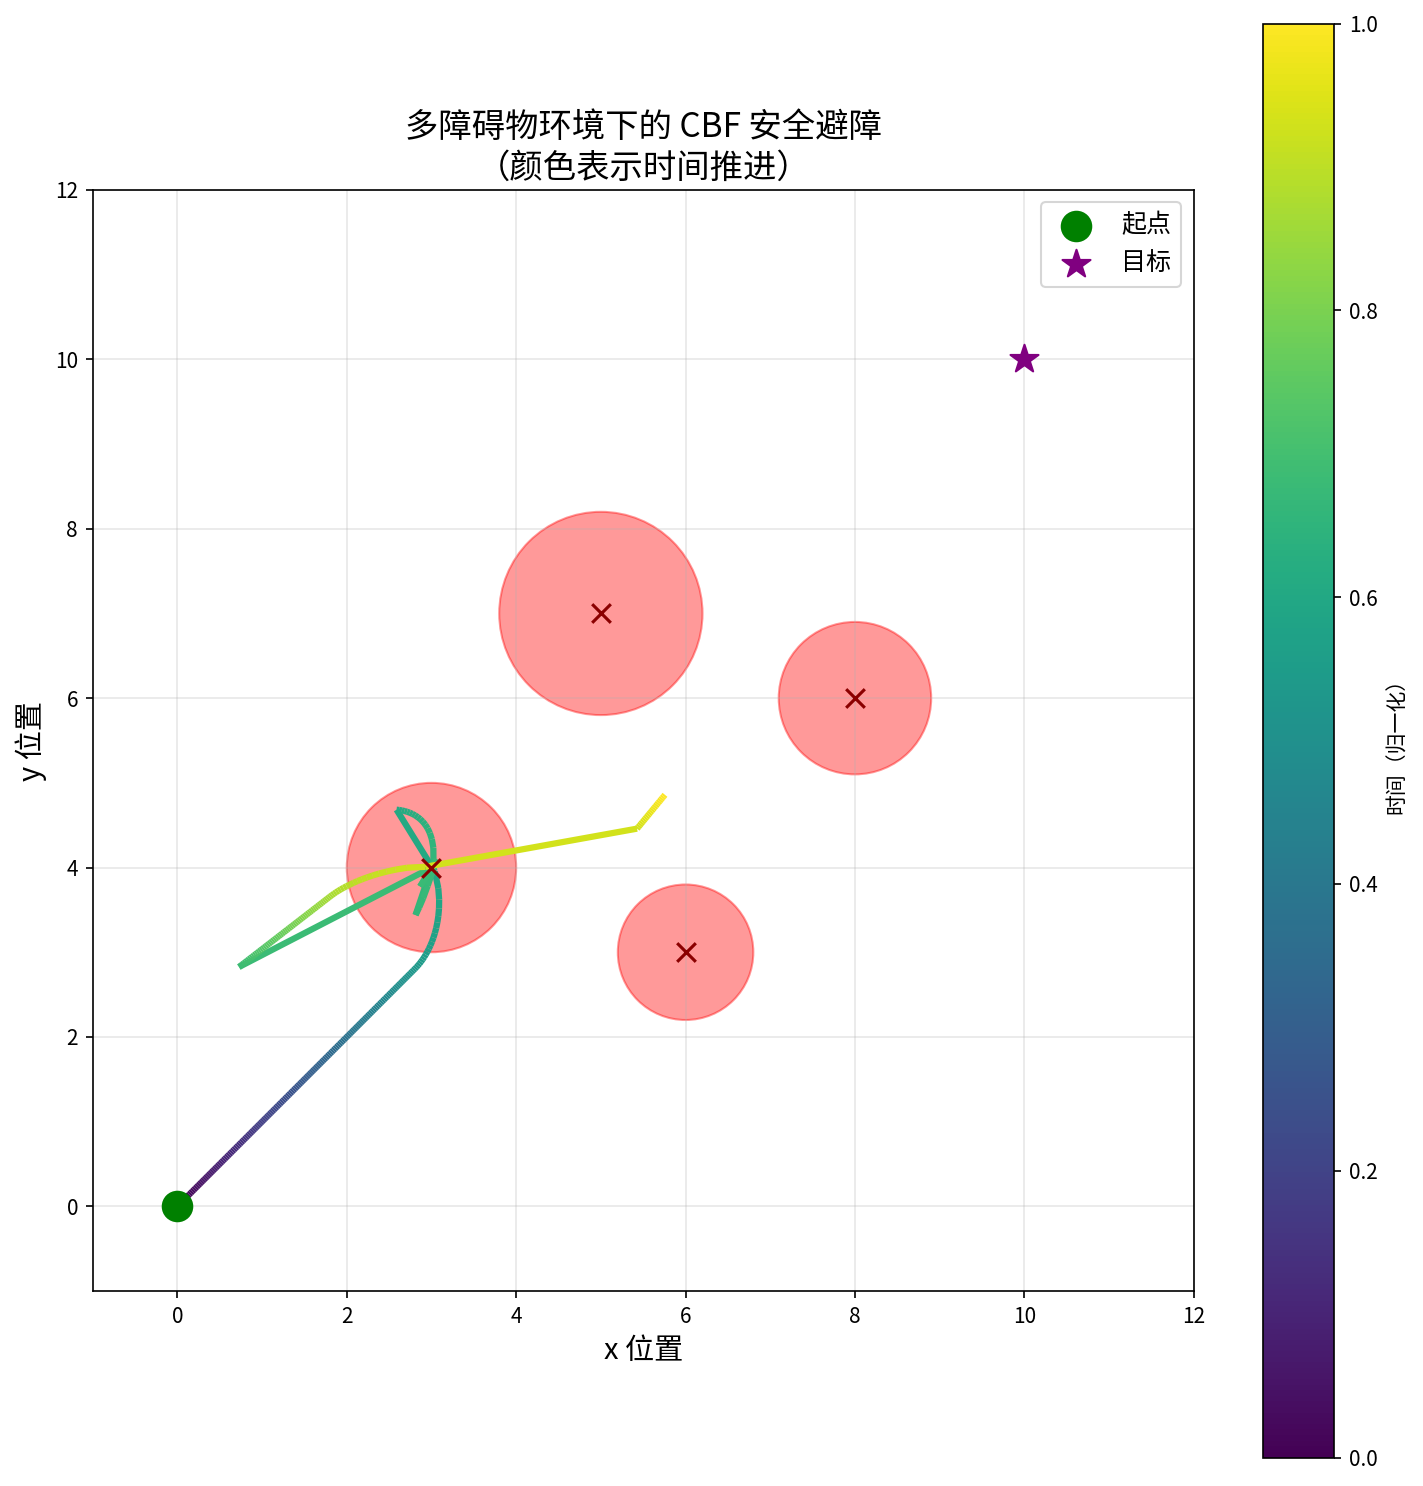
\includegraphics[width=0.75\textwidth]{figs_chap16/multi_obstacle.png}

\caption{多障碍物环境下的CBF避障。智能体从起点出发，自动规划路径绕过所有障碍物到达目标。颜色深浅表示时间推进。}

\label{fig:multi_obstacle}

\end{figure}

 

CBF方法可以自然地扩展到\textbf{多障碍物}场景：对每个障碍物定义一个障碍函数$h_i(x)$，然后在控制器中同时满足所有约束。

 

\begin{algorithm}[H]
\caption{CBF安全控制器伪代码}
\begin{algorithmic}[1]
\Require 当前位置 $x$，目标位置 $x_{\text{goal}}$，障碍物位置 $x_{\text{obs}}$，安全距离 $d$
\State \textbf{// 第一步：计算标称控制（朝目标走）}
\State $u_{\text{ref}} \gets \text{方向}(x_{\text{goal}} - x) \times \text{速度}$
\State \textbf{// 第二步：计算障碍函数及其梯度}
\State $h \gets \|x - x_{\text{obs}}\|^2 - d^2$ \Comment{正表示安全，负表示危险}
\State $\nabla h \gets 2(x - x_{\text{obs}})$ \Comment{指向远离障碍物的方向}
\State \textbf{// 第三步：检查安全约束}
\If{$\nabla h \cdot u_{\text{ref}} + \alpha \cdot h \geq 0$}
    \State \textbf{return} $u_{\text{ref}}$ \Comment{标称控制已经安全，无需修正}
\EndIf
\State \textbf{// 第四步：计算安全修正}
\State $\lambda \gets -\frac{\nabla h \cdot u_{\text{ref}} + \alpha \cdot h}{\|\nabla h\|^2}$
\State $u_{\text{safe}} \gets u_{\text{ref}} - \lambda \cdot \nabla h$ \Comment{沿梯度方向修正}
\State \textbf{return} $u_{\text{safe}}$
\end{algorithmic}
\end{algorithm}

 

% ====================================================================================

\section{可微物理：当牛顿定律变成计算图}

% ====================================================================================

 

\subsection{从黑盒到白盒}

 

传统的物理仿真器（如游戏引擎）是\textbf{黑盒}：你输入状态和控制，它输出下一个状态，但你无法知道"输出对输入的导数是多少"。

 

\textbf{可微物理}（Differentiable Physics）的思想是：把物理定律写成\textbf{可自动微分}的计算图。

 

\begin{definition}[可微物理仿真器]

可微物理仿真器将物理仿真实现为：

\begin{equation}
    x_{t+1} = \text{PhysicsStep}(x_t, u_t; \theta)
\end{equation}

其中$\theta$是物理参数（质量、刚度、摩擦系数等），整个函数对$(x_t, u_t, \theta)$都是\textbf{可微的}——可以计算梯度！

\end{definition}

 

\begin{example}[为什么需要可微？]

想象你在训练一个机器人走路：

\begin{itemize}

    \item 你有一个策略网络$\pi_\theta$，输出每个关节的力矩

    \item 物理仿真器计算机器人的运动

    \item 你想最小化"摔倒次数"

\end{itemize}

 

\textbf{传统方法}（强化学习）：随机尝试，看哪个好，很慢。

 

\textbf{可微物理}：直接计算"如果我改变策略参数，摔倒次数会怎么变"——梯度下降，很快。

\end{example}

 

\begin{advantage}[可微物理的三大优势]

\textbf{1. 策略优化}——直接优化策略参数：

\begin{equation}
    \theta^* = \arg\min_\theta \mathcal{L}(\text{Simulate}(\pi_\theta))
\end{equation}

用梯度下降代替随机搜索！

 

\textbf{2. 系统辨识}——从观测数据学习物理参数：

\begin{equation}
    \phi^* = \arg\min_\phi \|x_{\text{真实}} - x_{\text{仿真}}(\phi)\|^2
\end{equation}

给定轨迹数据，反推质量、摩擦系数等。

 

\textbf{3. Sim-to-Real迁移}——同时优化策略和物理参数，缩小仿真与现实的差距。

\end{advantage}

 

\subsection{实验：弹簧-质点系统的可微仿真}

 

让我们用一个简单的例子来说明可微物理的威力：\textbf{弹簧-质点系统}。

 

物理方程：

\begin{equation}
    m\ddot{x} = -kx - c\dot{x} + u
\end{equation}

其中：

\begin{itemize}

    \item $m$：质量

    \item $k$：弹簧刚度

    \item $c$：阻尼系数

    \item $u$：外力（控制输入）

\end{itemize}

 

\begin{figure}[htbp]

\centering

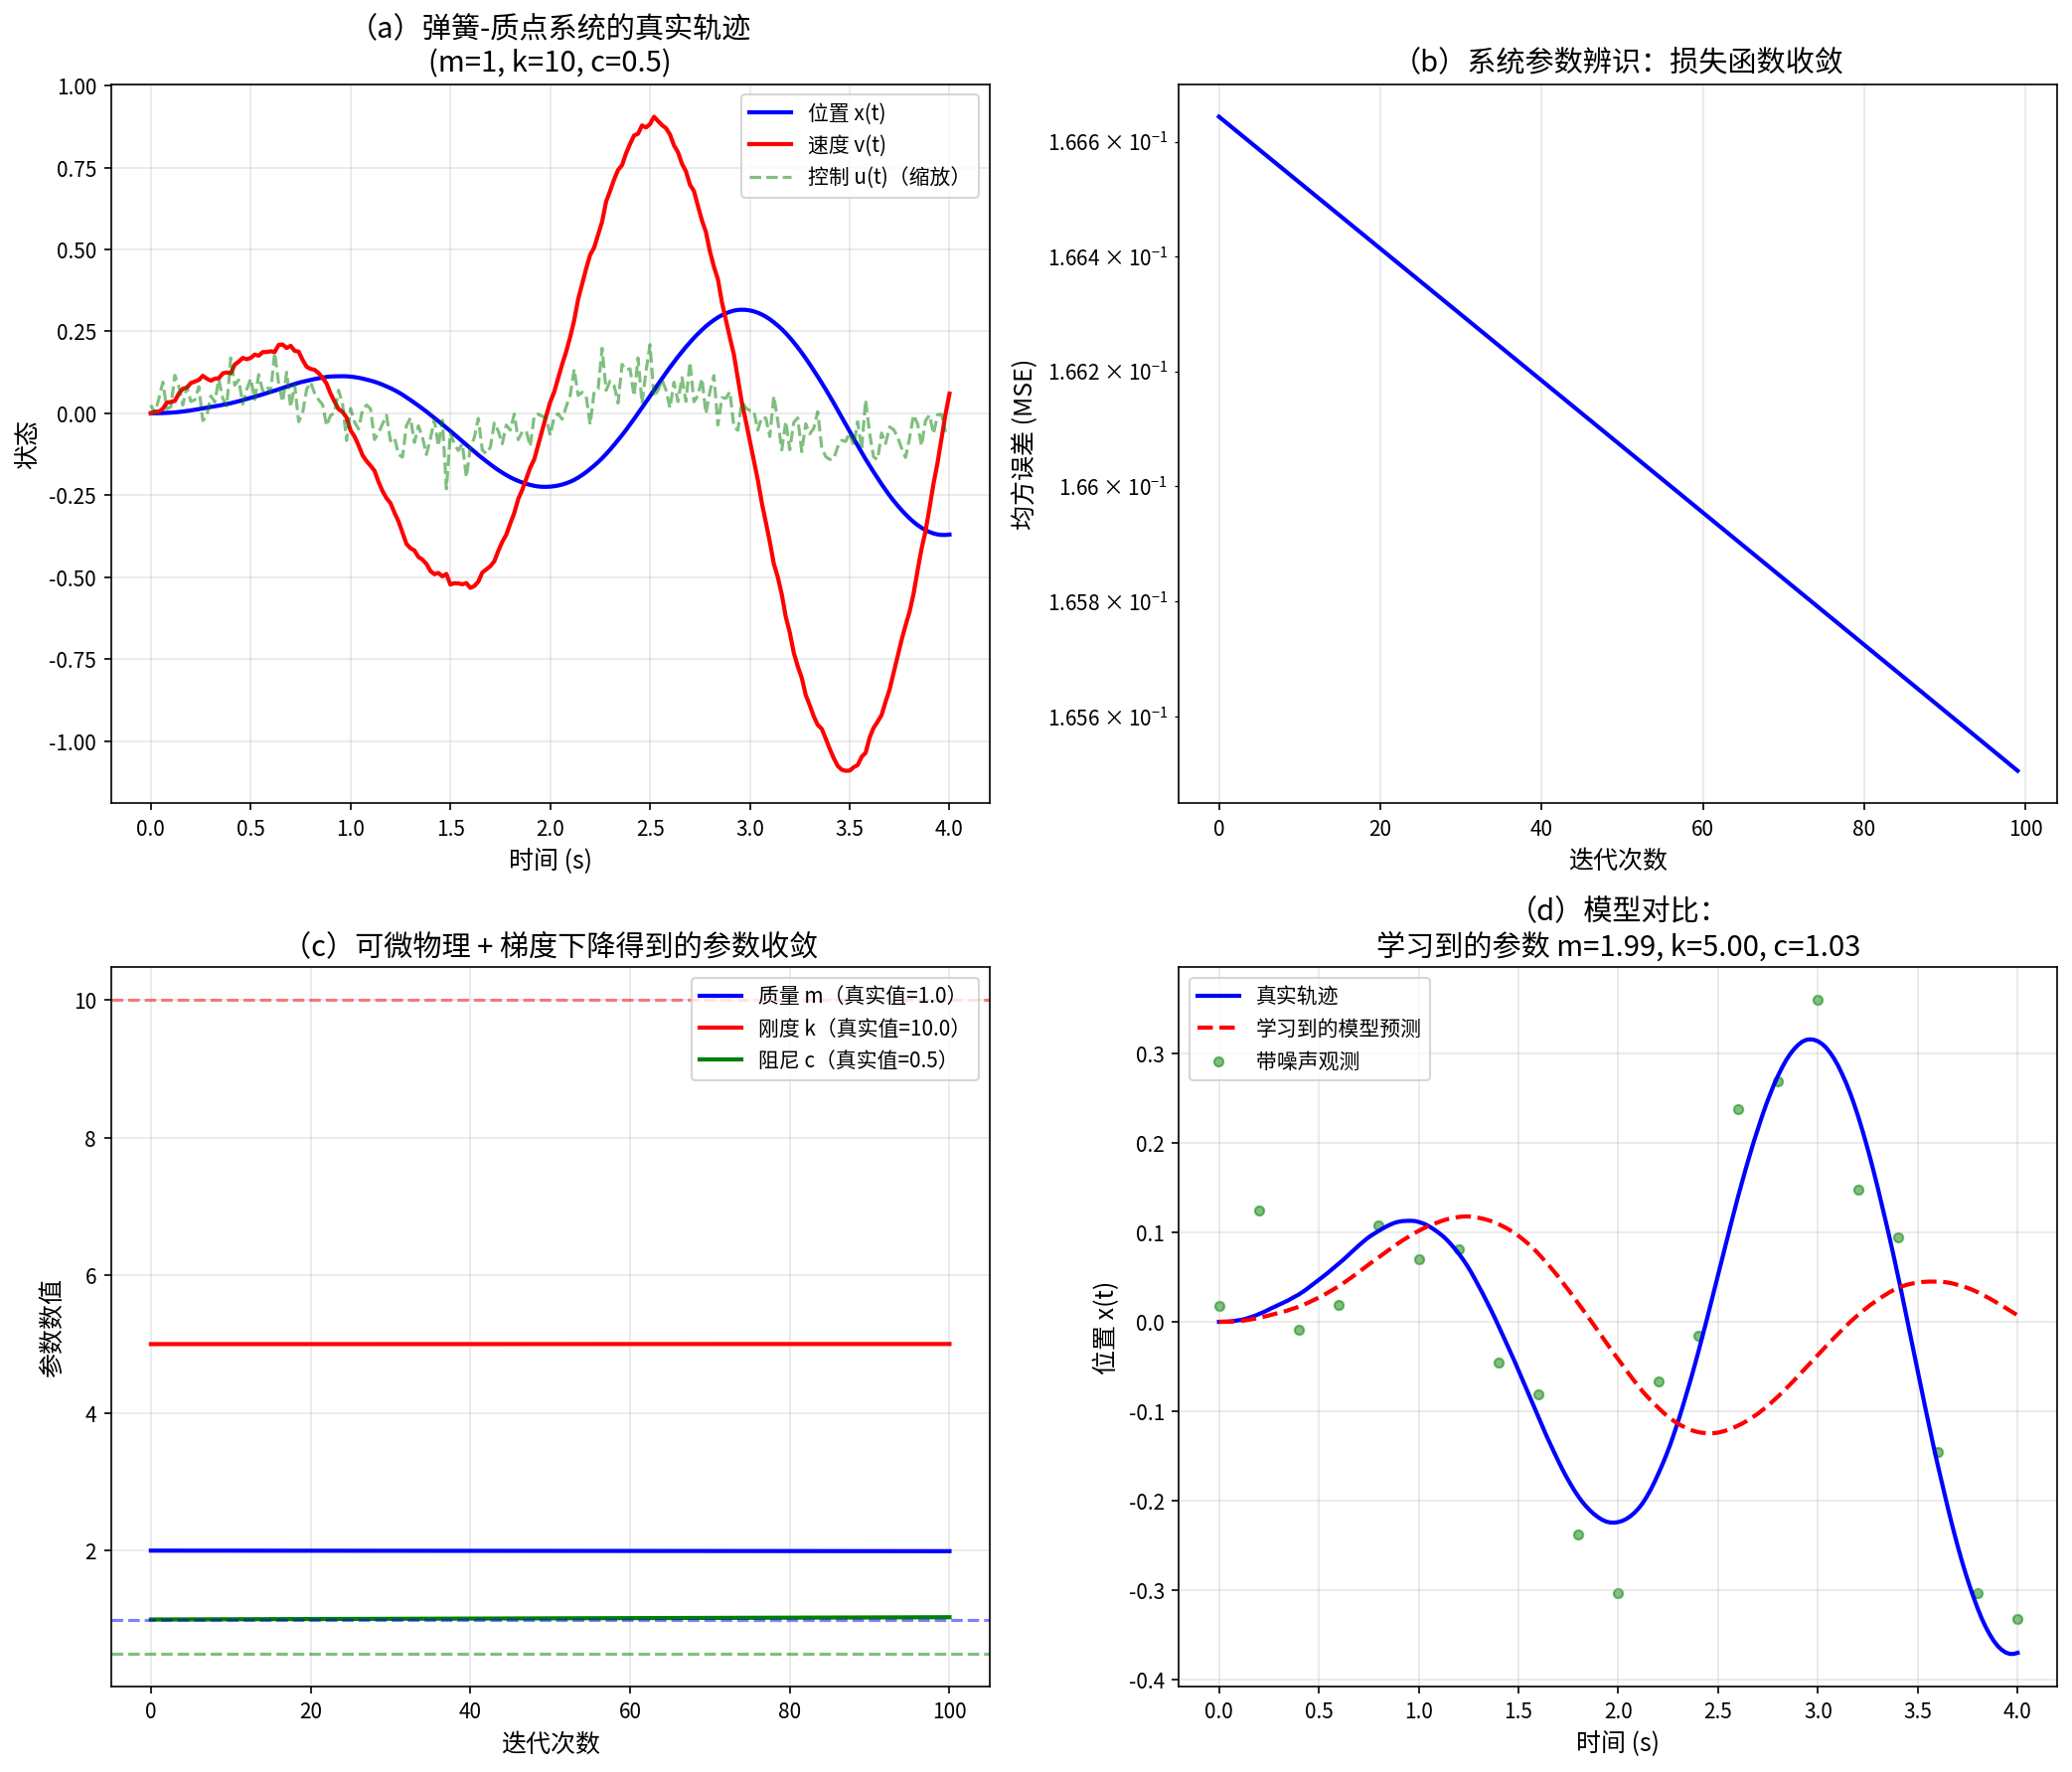
\includegraphics[width=0.95\textwidth]{figs_chap16/differentiable_physics.png}

\caption{可微物理系统辨识实验。(a)弹簧-质点系统的真实轨迹（$m=1, k=10, c=0.5$）；(b)损失函数随迭代下降；(c)三个物理参数逐渐收敛到真值；(d)学习到的模型能准确预测轨迹。}

\label{fig:differentiable_physics}

\end{figure}

 

\textbf{实验设置}：

\begin{itemize}

    \item 真实参数：$m=1, k=10, c=0.5$

    \item 初始猜测：$m=2, k=5, c=1$（故意猜错）

    \item 目标：从带噪声的观测数据中恢复真实参数

\end{itemize}

 

\textbf{实验结果分析}：

\begin{enumerate}

    \item \textbf{损失下降}：均方误差从初始值迅速下降两个数量级

    \item \textbf{参数收敛}：经过100次迭代，三个参数都接近真值

    \item \textbf{模型准确}：学到的模型（红色虚线）与真实轨迹（蓝色实线）高度吻合

\end{enumerate}

 

这个实验展示了可微物理的核心能力：\textbf{从数据中学习物理参数}。在更复杂的场景中（如机器人、流体），同样的方法可以用来校准仿真器，使其更接近真实世界。

 

\subsection{相空间：理解动力系统的窗口}

 

\begin{definition}[相空间——另一种看世界的方式]

对于一个力学系统，\textbf{相空间}是由位置$x$和速度$v$组成的空间。系统的状态是相空间中的一个点，随时间演化形成一条\textbf{轨迹}。

\end{definition}

 

\begin{figure}[htbp]

\centering

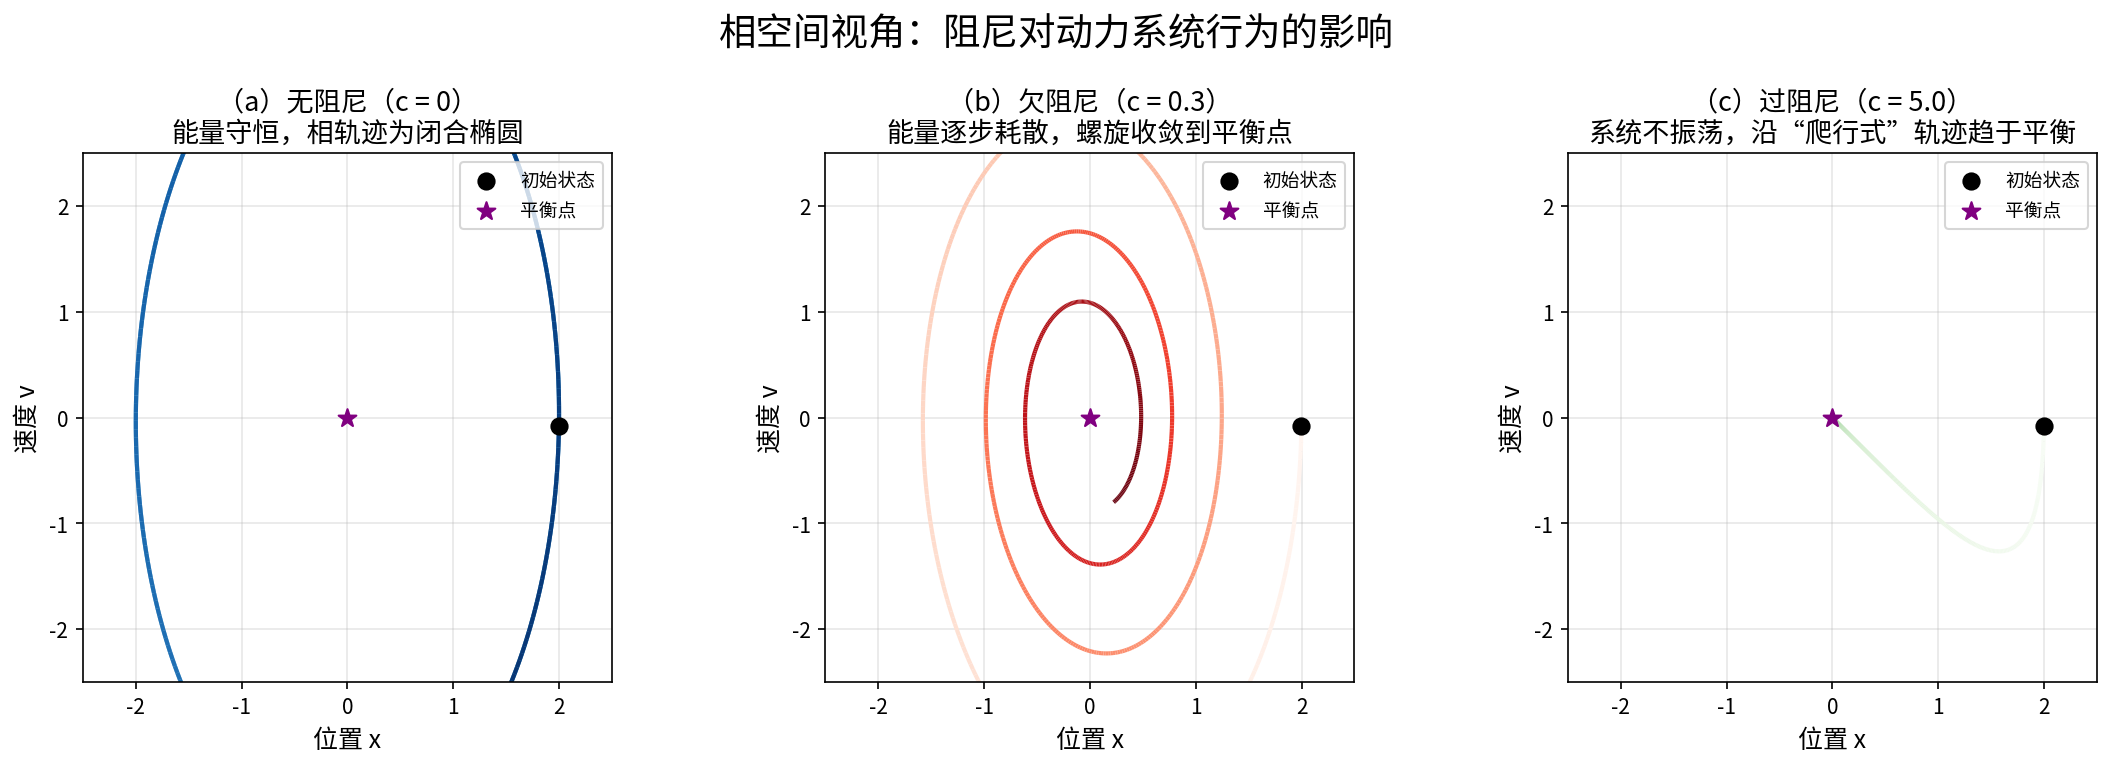
\includegraphics[width=0.95\textwidth]{figs_chap16/phase_space.png}

\caption{弹簧-质点系统的相空间轨迹。(a)无阻尼：能量守恒，轨迹是闭合的椭圆；(b)欠阻尼：能量逐渐耗散，轨迹螺旋趋向平衡点；(c)过阻尼：系统"懒洋洋"地直接趋向平衡点。}

\label{fig:phase_space}

\end{figure}

 

\textbf{相空间的物理意义}：

\begin{itemize}

    \item \textbf{无阻尼}（$c=0$）：总能量$E = \frac{1}{2}mv^2 + \frac{1}{2}kx^2$守恒，轨迹是椭圆

    \item \textbf{欠阻尼}（$c$较小）：能量逐渐耗散，轨迹螺旋向内

    \item \textbf{过阻尼}（$c$较大）：系统被"拖住"，缓慢趋向平衡

\end{itemize}

 

相空间是理解动力系统的重要工具——它让我们"一眼看出"系统的长期行为。

 

% ====================================================================================

\section{终极猜想：自由能原理与智能的统一理论}

% ====================================================================================

 

\marginnote{\textbf{Karl Friston}(1959--)：英国神经科学家，伦敦大学学院教授，英国皇家学会院士。他是世界上被引用最多的神经科学家，h-index超过250。他发明了脑成像分析的标准工具SPM，2000年代后致力于自由能原理，试图用单一数学框架统一大脑的感知、学习、决策。}

 

在本章的最后，让我们探讨一个大胆的问题：\textbf{智能的本质是什么？}

 

\subsection{惊奇最小化：一个统一的原理}

 

Karl Friston提出的\textbf{自由能原理}（Free Energy Principle）给出了一个优雅的答案：

 

\begin{philosophy}

\textbf{核心观点}：生命体（智能体）存在的目的，就是\textbf{最小化变分自由能}。

 

用更直白的话说：智能体试图\textbf{最小化惊奇}（Surprise）——让世界的行为符合自己的预期。

\end{philosophy}

 

\begin{example}[什么是"惊奇"？]

\begin{itemize}

    \item 你预期太阳从东边升起——太阳真的从东边升起——\textbf{不惊奇}

    \item 你预期房间里有椅子——椅子还在——\textbf{不惊奇}

    \item 你预期咖啡是热的——喝了一口是冰的——\textbf{惊奇！}

\end{itemize}

 

"惊奇"的数学定义是：$\text{惊奇} = -\log P(\text{观测})$

 

观测越不可能（越意外），惊奇越大。

\end{example}

 

\begin{definition}[变分自由能——稍微技术一点]

给定观测$o$和内部状态$s$（智能体的"信念"），\textbf{变分自由能}定义为：

\begin{equation}
    F = \E_{q(s)}[\log q(s) - \log p(s, o)]
\end{equation}

这可以分解为两部分：

\begin{equation}
    F = \underbrace{\text{KL}(q(s) \| p(s|o))}_{\text{信念与真实的差距}} + \underbrace{(-\log p(o))}_{\text{惊奇}}
\end{equation}

\end{definition}

 

\subsection{感知与行动的统一}

 

自由能原理最优美的地方在于：它用\textbf{同一个目标函数}统一了\textbf{感知}和\textbf{行动}。

 

\begin{figure}[htbp]

\centering

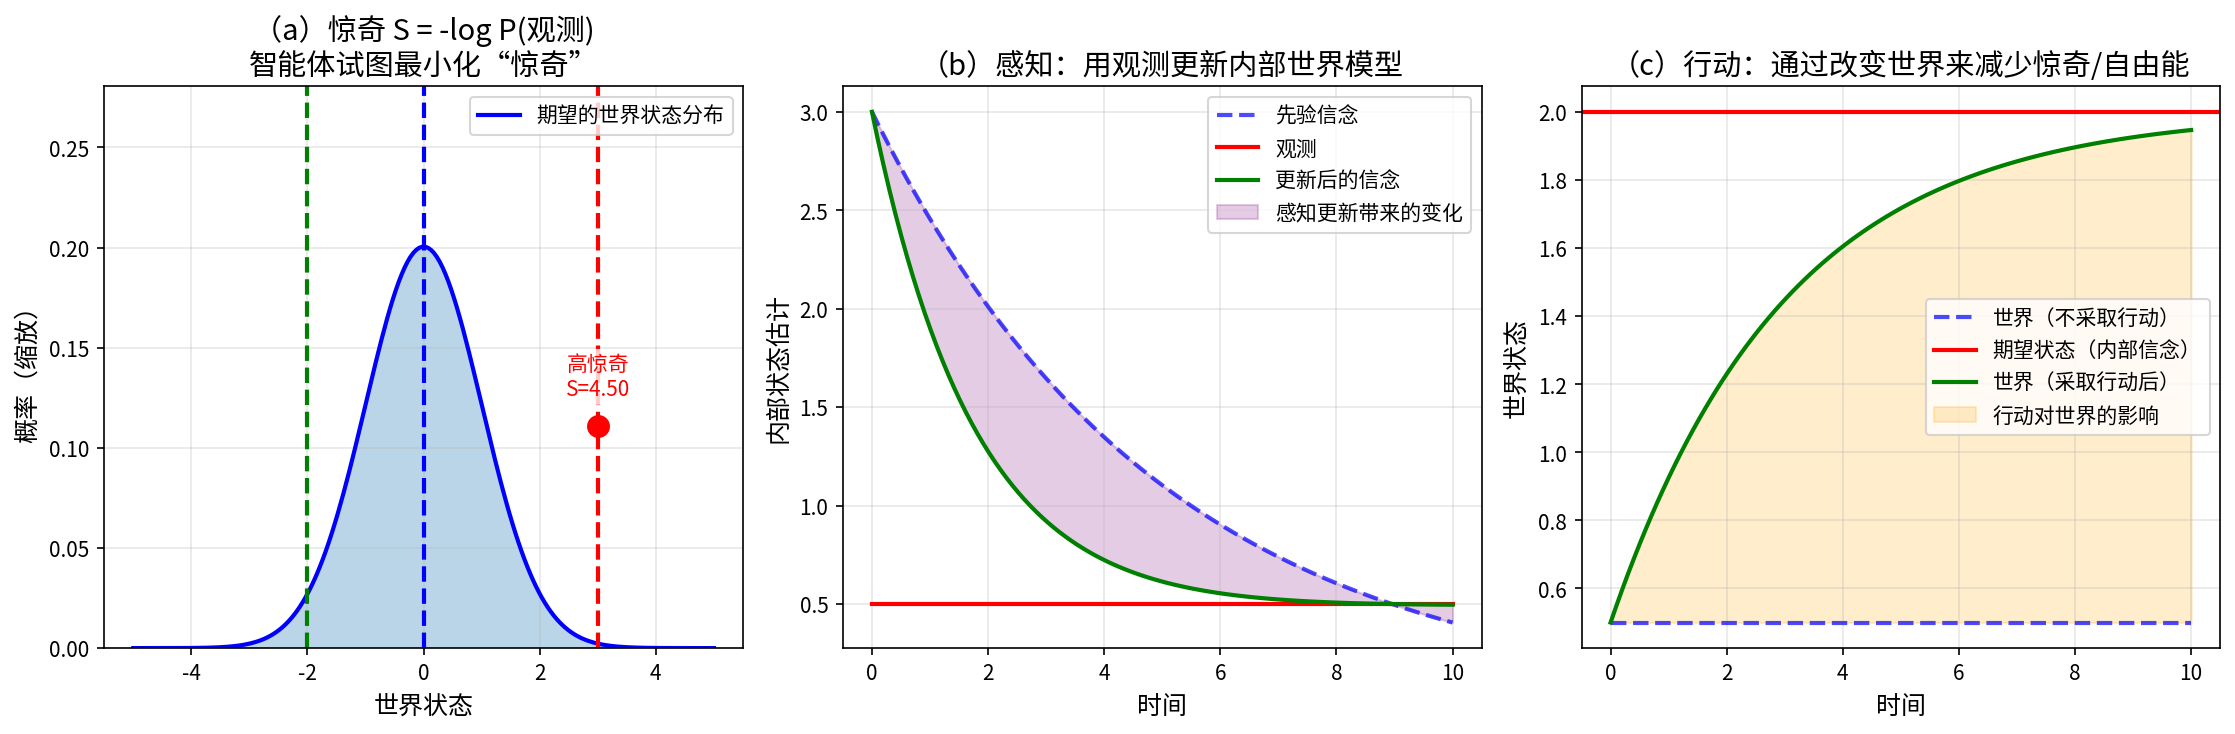
\includegraphics[width=0.95\textwidth]{figs_chap16/free_energy.png}

\caption{自由能原理示意图。(a)惊奇的定义：观测越偏离预期，惊奇越大；(b)感知：更新信念使之匹配观测；(c)行动：改变世界使之匹配信念。两者都在最小化惊奇！}

\label{fig:free_energy}

\end{figure}

 

\begin{keyformula}[title=感知与行动的统一]

\textbf{感知}（Perception）：更新内部信念$s$以最小化自由能

\begin{equation}
    s^* = \arg\min_s F(s, o) \quad \text{（"我看到了什么？更新我的信念"）}
\end{equation}

 

\textbf{行动}（Action）：改变世界状态以最小化\textbf{期望}自由能

\begin{equation}
    a^* = \arg\min_a \E_{p(o|a)}[F(s, o)] \quad \text{（"世界不符合预期？改变它！"）}
\end{equation}

 

两者都是在最小化"惊奇"——感知通过改变信念，行动通过改变世界！

\end{keyformula}

 

\begin{example}[为什么人在黑暗中感到不安？]

用自由能原理解释：

\begin{itemize}

    \item 在黑暗中，视觉输入的不确定性很高

    \item 高不确定性 = 难以预测 = 高惊奇

    \item 智能体天生"不喜欢"惊奇

    \item 所以人会感到不安，并采取行动（开灯、走到明亮处）来减少不确定性

\end{itemize}

\end{example}

 


 

% ====================================================================================

\section{习题}

% ====================================================================================

 

\subsection{概念题}

 

\begin{exercise}[世界模型的范式比较]

比较生成式世界模型和JEPA两种范式：

\begin{enumerate}

    \item 用自己的话解释：为什么LeCun认为"预测像素是浪费算力"？

    \item 从"约束优化"的角度，两者的目标函数有什么不同？

    \item 举一个生活中的例子，说明"学习本质"比"记忆细节"更重要。

\end{enumerate}

\end{exercise}

 

\begin{exercise}[CBF的物理意义]

考虑一个机器人在房间里移动，房间中央有一根柱子。

\begin{enumerate}

    \item 写出障碍函数$h(x)$的表达式（设机器人位置为$x$，柱子位置为$x_c$，安全距离为$r$）。

    \item 解释：为什么条件$\dot{h} \geq -\alpha h$能保证安全？

    \item CBF中的$\lambda^*$和拉格朗日力学中的约束力$\lambda$有什么相似之处？

\end{enumerate}

\end{exercise}

 

\begin{exercise}[自由能原理]

用自由能原理解释以下现象：

\begin{enumerate}

    \item 为什么人在黑暗的房间里会感到不安？

    \item 为什么我们喜欢有规律、可预测的生活？

    \item "好奇心"如何用自由能原理解释？（提示：探索可以减少未来的不确定性）

\end{enumerate}

\end{exercise}

 

\subsection{计算题}

 

\begin{exercise}[简单的CBF计算]

设系统状态$x \in \R$，动力学为$\dot{x} = u$（控制直接决定速度），障碍函数$h(x) = x - 1$（不能进入$x < 1$的区域）。

\begin{enumerate}

    \item 写出CBF条件$\dot{h} \geq -\alpha h$的具体形式。

    \item 如果标称控制$u_{\text{ref}} = -1$（朝危险方向走），当$x = 2$时，CBF会如何修正？

    \item 当$x = 1.1$时呢？

\end{enumerate}

\end{exercise}

 

\begin{exercise}[相空间分析]

对于弹簧-质点系统$m\ddot{x} = -kx - c\dot{x}$：

\begin{enumerate}

    \item 写出相空间$(x, v)$中的动力学方程。

    \item 当$c = 0$时，证明能量$E = \frac{1}{2}mv^2 + \frac{1}{2}kx^2$守恒。

    \item 当$c > 0$时，证明$\frac{dE}{dt} \leq 0$（能量只能减少）。

\end{enumerate}

\end{exercise}

 

\subsection{思考题}

 

\begin{exercise}[开放讨论]

本章提出"智能 = 在约束下寻找最优"。你认为这个观点能解释人类智能吗？有什么局限性？

\end{exercise}

% ====================================================================================
\section*{本章结语：从牛顿到智能}
\addcontentsline{toc}{section}{本章结语}
% ====================================================================================

\vspace{0.5cm}

当牛顿在1687年写下$F = ma$时，他大概不会想到，这个简单的方程会成为理解智能的钥匙。

\vspace{0.3cm}

当拉格朗日在1788年用变分法重写力学时，他大概不会想到，他的$\lambda$乘子会在300年后被用来训练神经网络、控制机器人、理解大脑。

\vspace{0.3cm}

而今天，当我们站在人工智能革命的浪潮中，回望这本书走过的旅程：

\begin{itemize}
    \item 从\textbf{第一章}的KKT条件，到\textbf{第十章}的强化学习
    \item 从\textbf{有限元}的$KU=F$，到\textbf{PINN}的物理信息损失
    \item 从\textbf{单智能体}的最优控制，到\textbf{多智能体}的纳什均衡
    \item 从\textbf{经典力学}的约束力，到\textbf{世界模型}的潜空间动力学
\end{itemize}

我们发现，所有这些看似迥异的领域，竟然都在诉说同一个故事：

\begin{keyformula}[title=全书的核心信息]
\begin{center}
\Large
\textbf{智能 = 在约束下寻找最优}
\end{center}

\vspace{0.3cm}

无论是石头滚下山坡，还是AlphaGo落子博弈；无论是单摆的简谐振动，还是GPT生成流畅的文字——它们都在做同一件事：在各自的约束条件下，寻找某种意义上的"最优解"。

\vspace{0.3cm}

\textbf{约束}定义了可能性的边界，\textbf{优化}选择了边界内的最佳路径。

\textbf{$\lambda$}不只是数学技巧，它是约束的"价格"，是物理的"力"，是信息的"代价"。
\end{keyformula}

\vspace{0.5cm}

\begin{philosophy}
\textbf{给读者的临别赠言}

\vspace{0.3cm}

如果你是大二的学生，正站在科学与工程的分岔路口，希望这本书能给你一个统一的视角：不要把物理、数学、计算机看成孤立的学科，它们是同一座大厦的不同房间。

\vspace{0.3cm}

当你下次遇到一个复杂问题时，不妨问自己三个问题：

\begin{enumerate}
    \item \textbf{目标是什么？}——我想最大化/最小化什么？
    \item \textbf{约束是什么？}——什么条件必须满足？
    \item \textbf{$\lambda$代表什么？}——约束的代价/价格/力是什么？
\end{enumerate}

这三个问题，能帮你把任何复杂问题，翻译成你已经熟悉的数学语言。
\end{philosophy}

\vspace{0.8cm}

\begin{center}
\Large
\textit{愿你在约束中找到自由，在优化中发现智慧。}

\vspace{0.5cm}

\normalsize
\textbf{全书完}
\end{center}   % 第16章：展望

% ####################################################################################
%                              全书总结
% ####################################################################################

\chapter*{全书总结：约束优化的统一视角}
\addcontentsline{toc}{chapter}{全书总结}

我们从一个简单的问题开始：
\begin{quote}
\textit{如何在满足约束的条件下，最大化（或最小化）一个目标？}
\end{quote}

拉格朗日的天才在于：引入乘子$\lambda$，把约束"吸收"进目标函数：
\begin{equation}
L(x, \lambda) = f(x) + \lambda^T g(x)
\end{equation}

这个简单的技巧，竟然能统一如此多的领域：

\begin{center}
\begin{tabular}{c|c|c}
\toprule
\textbf{领域} & \textbf{目标} & \textbf{$\lambda$的意义} \\
\midrule
经济学 & 效用最大化 & 边际价格 \\
力学 & 最小作用量 & 约束力 \\
有限元 & 能量最小 & 节点力 \\
信息论 & 最大熵 & 每比特代价 \\
控制 & 轨迹优化 & 协态变量 \\
机器学习 & 损失最小 & 梯度递推 \\
博弈论 & 纳什均衡 & 联合最优性 \\
\bottomrule
\end{tabular}
\end{center}

\vspace{1em}

\textbf{核心信息}：当你在任何领域遇到"有条件的优化"问题时，都可以用约束优化的框架来思考。
$\lambda$不只是数学上的"技巧"，它有深刻的物理/经济/信息含义——它度量了约束的"价格"。

希望这本书能帮助你建立这种统一的思维方式。当你下次看到一个复杂的问题时，
不妨问自己：\textbf{这里的约束是什么？$\lambda$代表什么？}




 



\begin{keyinsight}

\textbf{贯穿全书的数学之美}：

 

无论是单摆的运动、PDE的解、机器人的控制，还是智能体的决策，它们都可以用同一个数学框架来理解：

 

\begin{center}

\fbox{\Large 在约束下寻找最优}

\end{center}

 

这就是物理学与人工智能的深刻统一。

\end{keyinsight}

 

% ====================================================================================

\section*{结语：约束中的自由}

% ====================================================================================

 

\vspace{1cm}

 

当我们回顾这本书，从最简单的$F = ma$，到求解数百万参数的神经网络；从拉格朗日的$\lambda$乘子，到控制机器人的障碍函数。我们发现，人类理解世界的方式惊人地一致：

 

\begin{center}

\textit{世界是混乱的，但它是被约束的。}

\end{center}

 

物理定律是自然的\textbf{硬约束}——质能守恒、熵增原理、光速极限。

 

伦理道德是社会的\textbf{软约束}——法律、规范、价值观。

 

而\textbf{智能}（Intelligence），或许就是在这些重重约束的夹缝中，\textbf{寻找最优解的那道光}。

 

\vspace{0.5cm}

 

拉格朗日在1788年写下《解析力学》时，可能没有想到他的乘子会被用来训练神经网络。

 

香农在1948年创立信息论时，可能没有想到"惊奇最小化"会成为理解大脑的钥匙。

 

而今天的我们，站在巨人的肩膀上，正在用这些古老而优美的数学工具，构建能够感知、思考、行动的智能系统。

 

\vspace{0.5cm}

 

\begin{center}

\textit{希望这本书能让你在未来的AI研究中，\\
透过复杂的代码和架构，\\
看到那贯穿始终的数学本质。}

\end{center}

 

\vspace{2cm}

% ====================================================================================
\chapter*{附录：核心概念索引}
\addcontentsline{toc}{chapter}{附录：核心概念索引}
% ====================================================================================

本附录提供全书核心概念的快速索引，帮助读者：
\begin{itemize}
    \item 查找概念的首次出现位置和完整定义
    \item 理解同一概念在不同章节中的不同形态
    \item 复习时快速定位关键内容
\end{itemize}

% ------------------------------------------------------------------------------------
\section*{核心概念跨章对照表}

\begin{center}
\renewcommand{\arraystretch}{1.6}
\small
\begin{tabular}{p{2.8cm}|p{2.2cm}|p{8cm}}
\toprule
\textbf{概念} & \textbf{首次出现} & \textbf{各章节中的形态} \\
\midrule

\textbf{拉格朗日乘子} $\lambda$
& 第1章
& \textbf{Ch1}: 约束的"影子价格" \newline
  \textbf{Ch5}: 对偶问题的变量 \newline
  \textbf{Ch6}: 最大熵分布的特征权重 \newline
  \textbf{Ch8}: 伴随变量（协态变量） \newline
  \textbf{Ch9}: 反向传播中的误差信号 \newline
  \textbf{Ch15}: 博弈论中的边际价值 \\
\midrule

\textbf{KKT条件}
& 第1章
& \textbf{Ch1}: 约束优化的必要条件 \newline
  \textbf{Ch5}: 强对偶性的充分条件 \newline
  \textbf{Ch7}: SVM的支持向量条件 \newline
  \textbf{Ch15}: 纳什均衡的刻画 \\
\midrule

\textbf{对偶性}
& 第5章
& \textbf{Ch5}: 原问题与对偶问题的关系 \newline
  \textbf{Ch6}: 最大熵 = 最小KL散度 \newline
  \textbf{Ch7}: SVM原问题与对偶问题 \\
\midrule

\textbf{梯度/导数}
& 第3章
& \textbf{Ch3}: 矩阵求导规则 \newline
  \textbf{Ch4}: 正则化项的梯度 \newline
  \textbf{Ch9}: 反向传播计算梯度 \newline
  \textbf{Ch16}: 可微物理中的梯度 \\
\midrule

\textbf{伴随方程/变量}
& 第8章
& \textbf{Ch8}: 最优控制中的协态方程 \newline
  \textbf{Ch9}: 神经网络的反向传播 \newline
  \textbf{Ch16}: 可微仿真中的梯度计算 \\
\midrule

\textbf{熵}
& 第6章
& \textbf{Ch6}: Shannon熵，信息量的期望 \newline
  \textbf{Ch6}: KL散度中的负熵项 \newline
  \textbf{Ch12-5}: 注意力中的熵惩罚 \\
\midrule

\textbf{Softmax}
& 第6章
& \textbf{Ch6}: 最大熵分布的形式 \newline
  \textbf{Ch9}: 分类器输出层 \newline
  \textbf{Ch12}: Attention的权重归一化 \\
\midrule

\textbf{注意力机制}
& 第12章
& \textbf{Ch12}: Query-Key-Value结构 \newline
  \textbf{Ch12-5}: FlashAttention优化 \newline
  \textbf{Ch12-5}: 多头注意力 \\
\midrule

\textbf{正则化}
& 第4章
& \textbf{Ch4}: L1/L2范数惩罚 \newline
  \textbf{Ch7}: SVM的间隔最大化 \newline
  \textbf{Ch12-5}: MoE的负载均衡损失 \\
\bottomrule
\end{tabular}
\end{center}

% ------------------------------------------------------------------------------------
\section*{核心概念快速定义}

\subsection*{A. 优化基础（第1-5章）}

\begin{description}
    \item[拉格朗日乘子 (Lagrange Multiplier)]
    约束优化中引入的辅助变量，表示约束放松一个单位时目标函数的改进量（"影子价格"）。
    \[
    \mathcal{L}(x, \lambda) = f(x) + \lambda g(x)
    \]

    \item[KKT条件 (Karush-Kuhn-Tucker Conditions)]
    约束优化问题最优解的必要条件，包括：
    \begin{enumerate}
        \item 梯度条件：$\nabla f + \sum \lambda_i \nabla g_i = 0$
        \item 可行性：$g_i(x) \leq 0$（或 $= 0$）
        \item 互补松弛：$\lambda_i g_i(x) = 0$
        \item 对偶可行：$\lambda_i \geq 0$（不等式约束）
    \end{enumerate}

    \item[对偶问题 (Dual Problem)]
    通过拉格朗日函数构造的另一个优化问题，提供原问题最优值的下界。强对偶性成立时，两者最优值相等。

    \item[凸优化 (Convex Optimization)]
    目标函数和可行域都是凸的优化问题。局部最优 = 全局最优，KKT条件是充分必要条件。
\end{description}

\subsection*{B. 信息与学习（第6-7章）}

\begin{description}
    \item[熵 (Entropy)]
    分布不确定性的度量，也是平均信息量：
    \[
    H(p) = -\sum_i p_i \log p_i
    \]

    \item[KL散度 (Kullback-Leibler Divergence)]
    两个分布之间的"差异"（非对称）：
    \[
    D_{KL}(P \| Q) = \sum_i p_i \log \frac{p_i}{q_i}
    \]

    \item[交叉熵 (Cross Entropy)]
    用分布 $Q$ 编码分布 $P$ 的平均比特数：
    \[
    H(P, Q) = -\sum_i p_i \log q_i = H(P) + D_{KL}(P \| Q)
    \]

    \item[Softmax函数]
    将实数向量转换为概率分布的函数，是最大熵分布的形式：
    \[
    p_i = \frac{e^{z_i}}{\sum_j e^{z_j}}
    \]

    \item[支持向量机 (SVM)]
    间隔最大化的分类器，对偶问题只依赖于支持向量。
\end{description}

\subsection*{C. 控制与动态（第8章、第16章）}

\begin{description}
    \item[最优控制 (Optimal Control)]
    选择控制输入 $u(t)$ 使得系统轨迹最优化某个目标泛函。

    \item[伴随方程 (Adjoint Equation)]
    描述"未来代价对当前状态的敏感度"的微分方程，从终点向起点反向求解：
    \[
    \dot{\lambda} = -\frac{\partial H}{\partial x}
    \]

    \item[哈密顿函数 (Hamiltonian)]
    综合目标函数和约束的函数：
    \[
    H(x, u, \lambda) = L(x, u) + \lambda^\top f(x, u)
    \]

    \item[可微仿真 (Differentiable Simulation)]
    物理仿真的可微分版本，允许通过反向传播计算控制输入的梯度。
\end{description}

\subsection*{D. 神经网络（第9章、第12章）}

\begin{description}
    \item[反向传播 (Backpropagation)]
    高效计算神经网络梯度的算法，本质是伴随方程的离散版本。

    \item[计算图 (Computational Graph)]
    表示计算过程的有向无环图，前向传播计算值，反向传播计算梯度。

    \item[Transformer]
    基于自注意力机制的神经网络架构，不使用循环或卷积。

    \item[注意力机制 (Attention)]
    根据Query和Key的相似度对Value加权求和：
    \[
    \text{Attention}(Q, K, V) = \text{softmax}\left(\frac{QK^\top}{\sqrt{d_k}}\right) V
    \]

    \item[FlashAttention]
    IO感知的注意力算法，通过分块计算减少内存访问。

    \item[MoE (Mixture of Experts)]
    稀疏激活的架构，每个输入只激活部分专家网络。
\end{description}

\subsection*{E. 多智能体（第15章）}

\begin{description}
    \item[纳什均衡 (Nash Equilibrium)]
    每个玩家都采用最优响应的策略组合，没有人有动机单方面偏离。

    \item[最优响应 (Best Response)]
    给定其他玩家策略时，最大化自己收益的策略。

    \item[Cournot竞争]
    企业同时选择产量的寡头竞争模型，纳什均衡通过KKT条件求解。
\end{description}

% ------------------------------------------------------------------------------------
\section*{概念演化图谱}

\begin{center}
\begin{tikzpicture}[
    node distance=1.8cm,
    concept/.style={rectangle, rounded corners, draw=blue!50, fill=blue!10,
                    text width=2.5cm, align=center, minimum height=1cm},
    arrow/.style={->, >=stealth, thick, blue!60}
]

% 第一行：基础
\node[concept] (lagrange) {拉格朗日乘子\\(Ch1)};
\node[concept, right=of lagrange] (kkt) {KKT条件\\(Ch1)};
\node[concept, right=of kkt] (dual) {对偶性\\(Ch5)};

% 第二行：分支应用
\node[concept, below=of lagrange] (adjoint) {伴随方程\\(Ch8)};
\node[concept, below=of kkt] (entropy) {最大熵\\(Ch6)};
\node[concept, below=of dual] (svm) {SVM\\(Ch7)};

% 第三行：现代应用
\node[concept, below=of adjoint] (bp) {反向传播\\(Ch9)};
\node[concept, below=of entropy] (softmax) {Softmax\\(Ch6,12)};
\node[concept, below=of svm] (nash) {纳什均衡\\(Ch15)};

% 第四行：前沿
\node[concept, below=of bp] (diffsim) {可微仿真\\(Ch16)};
\node[concept, below=of softmax] (attention) {注意力\\(Ch12)};

% 箭头
\draw[arrow] (lagrange) -- (kkt);
\draw[arrow] (kkt) -- (dual);
\draw[arrow] (lagrange) -- (adjoint);
\draw[arrow] (lagrange) -- (entropy);
\draw[arrow] (dual) -- (svm);
\draw[arrow] (adjoint) -- (bp);
\draw[arrow] (entropy) -- (softmax);
\draw[arrow] (kkt) -- (nash);
\draw[arrow] (bp) -- (diffsim);
\draw[arrow] (softmax) -- (attention);

% 虚线连接（表示概念联系）
\draw[dashed, gray] (adjoint) -- (bp);
\draw[dashed, gray] (bp) to[bend right=20] (diffsim);

\end{tikzpicture}
\end{center}

\vspace{0.5cm}
\begin{center}
\textit{箭头表示概念的继承/发展关系，虚线表示本质相同的不同表述。}
\end{center}

% ------------------------------------------------------------------------------------
\section*{本书的核心信息}

\begin{unification}[title=一个公式，多个化身]
拉格朗日函数的梯度条件
\[
\nabla_x \mathcal{L} = \nabla f + \lambda \nabla g = 0
\]
在不同领域有不同的名字：

\begin{center}
\renewcommand{\arraystretch}{1.4}
\begin{tabular}{l|l}
\toprule
\textbf{领域} & \textbf{名字} \\
\midrule
微积分 & 拉格朗日乘子法 \\
运筹学 & KKT条件 \\
物理学 & 哈密顿原理 \\
控制论 & 伴随方程 \\
机器学习 & 反向传播 \\
信息论 & 最大熵分布 \\
博弈论 & 纳什均衡条件 \\
\bottomrule
\end{tabular}
\end{center}

\textbf{理解了拉格朗日乘子的本质，就等于理解了它们的共同根源。}
\end{unification}

% ------------------------------------------------------------------------------------
\section*{章节速查}

\begin{center}
\renewcommand{\arraystretch}{1.3}
\begin{tabular}{c|l|l}
\toprule
\textbf{章} & \textbf{标题} & \textbf{核心关键词} \\
\midrule
1 & 从高数到约束优化 & 拉格朗日乘子、KKT条件、影子价格 \\
2 & 线性代数回顾 & 特征值、SVD、正定矩阵 \\
3 & 矩阵求导 & 链式法则、Jacobian、Hessian \\
4 & 范数与正则化 & L1/L2范数、稀疏性、过拟合 \\
5 & 凸优化与对偶 & 对偶问题、强对偶、凸集 \\
6 & 信息与编码 & 熵、KL散度、交叉熵、Softmax \\
7 & 支持向量机 & 间隔、核技巧、对偶形式 \\
8 & 最优控制 & 伴随方程、Pontryagin原理 \\
9 & 神经网络 & 反向传播、计算图、自动微分 \\
10 & 动态规划 & Bellman方程、值函数 \\
12 & Transformer & 自注意力、多头注意力 \\
12-5 & 高效计算 & FlashAttention、MoE \\
14 & 强化学习 & 策略梯度、Actor-Critic \\
15 & 多智能体 & 纳什均衡、博弈论 \\
16 & 世界模型 & 可微仿真、模型预测控制 \\
\bottomrule
\end{tabular}
\end{center}
  % 附录A：核心概念索引
% ====================================================================================
\appendixchapter{实验环境速成——服务器与环境配置}{实验环境速成}
% ====================================================================================

\sidenoteplain{本附录原是“大模型工程”一章（现附录C）的扩展阅读，给完全没有服务器使用经验的同学准备。如果你已经熟悉 Linux 和 Git，可以跳过前面的基础部分。}

\noindent\textit{本附录不讲数学。}它回答的是一个很实际的问题：当你的笔记本电脑跑不动第8--16章的实验时，怎样在实验室服务器或学校集群上把代码跑起来——连接服务器、配置环境、提交训练任务、把结果取回来。各节相互独立，随用随查。

% ------------------------------------------------------------------------------------
\section*{连接服务器：SSH基础}
\addcontentsline{toc}{section}{连接服务器：SSH基础}
% ------------------------------------------------------------------------------------

\paragraph{什么是SSH？}

SSH（Secure Shell）是连接远程服务器的标准方式。你在自己电脑上输入命令，实际在服务器上执行。

\paragraph{基本连接命令}\mbox{}\par\nopagebreak

\begin{lstlisting}[language=bash, caption=SSH连接服务器]
# 基本格式
ssh 用户名@服务器地址

# 示例：连接到实验室服务器
ssh zhangsan@192.168.1.100

# 如果服务器用非标准端口（比如2222）
ssh -p 2222 zhangsan@192.168.1.100

# 第一次连接会问你是否信任，输入 yes
\end{lstlisting}

\paragraph{免密登录配置}

每次输密码很烦，可以配置SSH密钥实现免密登录：

\begin{lstlisting}[language=bash, caption=配置SSH免密登录]
# 1. 在自己电脑上生成密钥（如果没有的话）
ssh-keygen -t rsa -b 4096
# 一路回车，使用默认设置

# 2. 把公钥复制到服务器
ssh-copy-id zhangsan@192.168.1.100
# 输入一次密码

# 3. 以后就可以直接连接，不用密码了
ssh zhangsan@192.168.1.100
\end{lstlisting}

\paragraph{SSH配置文件}

在 \texttt{\~/.ssh/config} 中配置常用服务器，以后连接更方便：

\begin{lstlisting}[language=bash, caption=SSH配置文件示例]
# 文件位置: ~/.ssh/config

# 实验室GPU服务器
Host lab
    HostName 192.168.1.100
    User zhangsan
    Port 22

# 学校计算集群
Host cluster
    HostName hpc.university.edu
    User s2024001
    Port 22

# 配置好后，直接用别名连接
# ssh lab
# ssh cluster
\end{lstlisting}

% ------------------------------------------------------------------------------------
\section*{Linux基础命令}
\addcontentsline{toc}{section}{Linux基础命令}
% ------------------------------------------------------------------------------------

服务器通常运行Linux系统（如Ubuntu）。这里列出最常用的命令：

\paragraph{文件与目录操作}\mbox{}\par\nopagebreak

\begin{table}[H]
\centering
\small
\renewcommand{\arraystretch}{1.3}
\begin{tabular}{l|l|l}
\toprule
\textbf{命令} & \textbf{功能} & \textbf{示例} \\
\midrule
\texttt{pwd} & 显示当前目录 & \texttt{pwd} \\
\texttt{ls} & 列出文件 & \texttt{ls -la}（显示详细信息） \\
\texttt{cd} & 切换目录 & \texttt{cd /home/user/project} \\
\texttt{mkdir} & 创建目录 & \texttt{mkdir -p data/train} \\
\texttt{cp} & 复制文件 & \texttt{cp file.txt backup/} \\
\texttt{mv} & 移动/重命名 & \texttt{mv old.txt new.txt} \\
\texttt{rm} & 删除文件 & \texttt{rm -rf folder/}（谨慎！） \\
\texttt{cat} & 查看文件内容 & \texttt{cat config.yaml} \\
\texttt{head/tail} & 查看开头/结尾 & \texttt{tail -f train.log}（实时查看） \\
\texttt{du} & 查看磁盘占用 & \texttt{du -sh *}（当前目录各文件大小） \\
\texttt{df} & 查看磁盘空间 & \texttt{df -h}（各分区剩余空间） \\
\bottomrule
\end{tabular}
\caption{常用文件操作命令}
\end{table}

\paragraph{进程与资源监控}\mbox{}\par\nopagebreak

\begin{table}[H]
\centering
\small
\renewcommand{\arraystretch}{1.3}
\begin{tabular}{l|l|l}
\toprule
\textbf{命令} & \textbf{功能} & \textbf{说明} \\
\midrule
\texttt{nvidia-smi} & 查看GPU状态 & 显存占用、温度、进程 \\
\texttt{watch -n 1 nvidia-smi} & 实时监控GPU & 每秒刷新 \\
\texttt{htop} & 查看CPU和内存 & 比\texttt{top}更友好 \\
\texttt{ps aux | grep python} & 查找Python进程 & 找到你的训练进程 \\
\texttt{kill PID} & 结束进程 & \texttt{kill -9 12345}（强制结束） \\
\bottomrule
\end{tabular}
\caption{进程监控命令}
\end{table}

\begin{figure}[htbp]
\centering
\begin{tikzpicture}[scale=0.9]
    % nvidia-smi 输出示意
    \node[draw, rectangle, fill=black!90, text=green!80, font=\ttfamily\scriptsize, 
          align=left, minimum width=12cm, minimum height=5cm] at (0, 0) {
+-----------------------------------------------------------------------------+\\
| NVIDIA-SMI 535.104.05   Driver Version: 535.104.05   CUDA Version: 12.2     |\\
|-------------------------------+----------------------+----------------------+\\
| GPU  Name        Persistence-M| Bus-Id        Disp.A | Volatile Uncorr. ECC |\\
| Fan  Temp  Perf  Pwr:Usage/Cap|         Memory-Usage | GPU-Util  Compute M. |\\
|===============================+======================+======================|\\
|   0  NVIDIA A100-SXM...  On   | 00000000:00:04.0 Off |                    0 |\\
| N/A   32C    P0    52W / 400W |  45231MiB / 81920MiB |      0\%      Default |\\
+-------------------------------+----------------------+----------------------+\\
|                                                                             |\\
| Processes:                                                                  |\\
|  GPU   GI   CI        PID   Type   Process name                  GPU Memory |\\
|        ID   ID                                                   Usage      |\\
|=============================================================================|\\
|    0   N/A  N/A     12345      C   python train.py                45200MiB |\\
+-----------------------------------------------------------------------------+
    };
\end{tikzpicture}
\caption{\texttt{nvidia-smi}输出示例：显示GPU型号、显存使用、运行中的进程}
\end{figure}

\paragraph{文件传输}\mbox{}\par\nopagebreak

\begin{lstlisting}[language=bash, caption=在本地和服务器之间传输文件]
# 从本地上传到服务器
scp local_file.py zhangsan@server:/home/zhangsan/project/

# 从服务器下载到本地
scp zhangsan@server:/home/zhangsan/results.csv ./

# 上传整个文件夹（-r 递归）
scp -r ./my_project zhangsan@server:/home/zhangsan/

# 如果配置了SSH config，可以用别名
scp local_file.py lab:/home/zhangsan/project/
\end{lstlisting}

% ------------------------------------------------------------------------------------
\section*{Git版本控制}
\addcontentsline{toc}{section}{Git版本控制}
% ------------------------------------------------------------------------------------

Git是代码版本管理的标准工具。即使只有你一个人写代码，也强烈建议用Git。

\paragraph{为什么要用Git？}

Git 记录你的每一次修改，所以任何时候都可以回退到之前的某个版本；有了这层保险，你就不必担心改坏代码——改坏了就退回去。它还解决了另一个很实际的问题：代码要在本地和服务器等多台机器之间来回同步，多人合作时还要合并各自的改动，靠手工拷贝文件很快就会乱套，而 Git 正是为此设计的。

\paragraph{Git基本工作流程}\mbox{}\par\nopagebreak

\begin{figure}[H]
\centering
\begin{tikzpicture}[>=stealth, scale=0.85,
    box/.style={draw, rounded corners, minimum width=2.2cm, minimum height=1cm, align=center}]
    
    % 三个区域
    \node[box, fill=blue!20] (work) at (0, 0) {工作目录\\Working};
    \node[box, fill=green!20] (stage) at (5, 0) {暂存区\\Staging};
    \node[box, fill=orange!20] (repo) at (10, 0) {本地仓库\\Repository};
    \node[box, fill=purple!20] (remote) at (10, -3) {远程仓库\\GitHub/GitLab};
    
    % 箭头
    \draw[->, thick] (work) -- node[above, font=\small] {\texttt{git add}} (stage);
    \draw[->, thick] (stage) -- node[above, font=\small] {\texttt{git commit}} (repo);
    \draw[->, thick] (repo) -- node[right, font=\small] {\texttt{git push}} (remote);
    \draw[->, thick] (remote) -- node[left, font=\small] {\texttt{git pull}} ++(-5, 0) -- (work);
    
\end{tikzpicture}
\caption{Git工作流程}
\end{figure}

\paragraph{常用Git命令}\mbox{}\par\nopagebreak

\begin{lstlisting}[language=bash, caption=Git常用命令]
# === 初始化 ===
git init                    # 在当前目录创建Git仓库
git clone <url>             # 克隆远程仓库

# === 日常使用 ===
git status                  # 查看当前状态（哪些文件改了）
git add .                   # 把所有修改添加到暂存区
git add train.py            # 只添加特定文件
git commit -m "描述信息"     # 提交，写清楚这次改了什么

# === 与远程同步 ===
git pull                    # 从远程拉取最新代码
git push                    # 把本地提交推送到远程

# === 查看历史 ===
git log --oneline           # 查看提交历史（简洁版）
git diff                    # 查看未暂存的修改
git diff --staged           # 查看已暂存的修改

# === 分支（进阶） ===
git branch                  # 查看分支
git checkout -b new_feature # 创建并切换到新分支
git merge new_feature       # 合并分支
\end{lstlisting}

\paragraph{典型工作流程示例}\mbox{}\par\nopagebreak

\begin{lstlisting}[language=bash, caption=一次完整的Git工作流程]
# 1. 开始工作前，先拉取最新代码
git pull

# 2. 写代码、做实验...

# 3. 查看改了哪些文件
git status

# 4. 添加修改
git add .

# 5. 提交，写清楚改了什么
git commit -m "增加学习率warmup功能"

# 6. 推送到远程（比如GitHub）
git push

# 现在你的代码就安全地保存在远程了！
\end{lstlisting}

\paragraph{.gitignore文件}

有些文件不应该加入Git（比如数据集、模型权重、临时文件）：

\begin{lstlisting}[language=bash, caption=.gitignore示例]
# .gitignore 文件内容

# 数据和模型（太大了）
data/
checkpoints/
*.pt
*.bin

# Python临时文件
__pycache__/
*.pyc
.ipynb_checkpoints/

# 环境和配置
.env
wandb/
outputs/

# 系统文件
.DS_Store
*.log
\end{lstlisting}

% ------------------------------------------------------------------------------------
\section*{Python环境管理：Conda}
\addcontentsline{toc}{section}{Python环境管理：Conda}
% ------------------------------------------------------------------------------------

服务器上可能有多个用户、多个项目，每个项目需要的Python版本和库可能不同。\textbf{Conda}帮你管理独立的Python环境。

\paragraph{为什么要用虚拟环境？}

不同项目常常需要不同版本的 PyTorch 和其他库，如果都装进同一个 Python 里，版本迟早会互相冲突，还会把系统自带的 Python 弄乱。虚拟环境把每个项目的依赖隔离开：各装各的版本，互不干扰；哪个环境出了问题，直接删掉重建就行，不会波及别的项目。

\paragraph{Conda基本命令}\mbox{}\par\nopagebreak

\begin{lstlisting}[language=bash, caption=Conda环境管理]
# === 创建环境 ===
conda create -n myenv python=3.10   # 创建名为myenv的环境，Python 3.10
conda activate myenv                 # 激活环境
conda deactivate                     # 退出环境

# === 查看环境 ===
conda env list                       # 列出所有环境
conda list                           # 列出当前环境的所有包

# === 安装包 ===
conda install numpy pandas           # 用conda安装
pip install torch transformers       # 用pip安装（conda没有的包）

# === 删除环境 ===
conda remove -n myenv --all          # 删除整个环境

# === 导出/导入环境 ===
conda env export > environment.yml   # 导出环境配置
conda env create -f environment.yml  # 从配置文件创建环境
\end{lstlisting}

\paragraph{典型深度学习环境配置}\mbox{}\par\nopagebreak

\begin{lstlisting}[language=bash, caption=配置一个深度学习环境]
# 1. 创建新环境
conda create -n llm python=3.10
conda activate llm

# 2. 安装PyTorch（去官网查对应CUDA版本的命令）
# https://pytorch.org/get-started/locally/
pip install torch torchvision torchaudio --index-url https://download.pytorch.org/whl/cu118

# 3. 安装常用库
pip install transformers datasets accelerate
pip install wandb tensorboard
pip install jupyter ipython

# 4. 验证安装
python -c "import torch; print(torch.cuda.is_available())"
# 应该输出 True
\end{lstlisting}

% ------------------------------------------------------------------------------------
\section*{CUDA 与 PyTorch 版本的坑}
\addcontentsline{toc}{section}{CUDA 与 PyTorch 版本的坑}
% ------------------------------------------------------------------------------------

\sidenoteplain{这一节是很多新手踩的最大坑：不理解CUDA版本、PyTorch版本、驱动版本之间的关系，随意升级，结果把组里老代码全搞挂了。}

在公用服务器上，\textbf{版本管理}是一个非常重要但经常被忽视的问题。理解下面这些概念，能帮你避免“一改配置全组遭殃”的惨剧。

\paragraph{三个版本的区别}\mbox{}\par\nopagebreak

\begin{table}[H]
\centering
\small
\renewcommand{\arraystretch}{1.4}
\begin{tabularx}{\textwidth}{l|X|l|l}
\toprule
\textbf{名称} & \textbf{是什么} & \textbf{谁负责安装} & \textbf{能否随意改} \\
\midrule
\textbf{NVIDIA驱动} & GPU的底层驱动 & 系统管理员 & \textcolor{red}{绝对不能！} \\
\textbf{CUDA Toolkit} & GPU编程工具包 & 系统或用户 & 谨慎（见下文） \\
\textbf{PyTorch CUDA版本} & PyTorch编译时用的CUDA & pip安装时选择 & 可以，但要匹配 \\
\bottomrule
\end{tabularx}
\caption{三种“CUDA版本”的区别}
\end{table}

\begin{keyidea}[版本兼容的关键原则]
三者的关系是分层的。\textbf{驱动}在最底层，同一台机器上只有一个；它向下兼容，所以驱动版本必须 $\geq$ CUDA Toolkit 版本。\textbf{CUDA Toolkit} 在中间，同一台机器上可以装多个版本。\textbf{PyTorch 的 CUDA 版本}在最上层，它必须与系统的 CUDA Toolkit 匹配。
\end{keyidea}

\paragraph{如何查看版本}\mbox{}\par\nopagebreak

\begin{lstlisting}[language=bash, caption=查看各种CUDA相关版本]
# 1. 查看NVIDIA驱动版本（nvidia-smi右上角）
nvidia-smi
# 输出: Driver Version: 535.104.05   CUDA Version: 12.2
#                                     ^^^^^^^^^^^^
#                        注意：这是驱动支持的最高CUDA版本，不是系统安装的CUDA

# 2. 查看系统安装的CUDA Toolkit版本
nvcc --version
# 输出: Cuda compilation tools, release 11.8, V11.8.89

# 3. 查看PyTorch使用的CUDA版本
python -c "import torch; print(torch.version.cuda)"
# 输出: 11.8

# 4. 验证PyTorch能否使用GPU
python -c "import torch; print(torch.cuda.is_available())"
# 输出: True  (如果是False，说明版本不匹配！)
\end{lstlisting}

\begin{remark}
\texttt{nvidia-smi}显示的“CUDA Version”容易让人误解。那是\textbf{驱动支持的最高CUDA版本}，不是你实际安装的CUDA版本。实际版本要用\texttt{nvcc --version}查看。
\end{remark}

\paragraph{什么是 \texttt{cuda:0}？}

当你写 \texttt{.to("cuda:0")} 时，\texttt{cuda:0}表示\textbf{第0号GPU}。

\begin{lstlisting}[language=Python, caption=GPU设备管理]
import torch

# 查看有几张GPU
print(torch.cuda.device_count())  # 比如输出 4，表示有4张卡

# 查看当前默认设备
print(torch.cuda.current_device())  # 通常是 0

# 把张量放到指定GPU
x = torch.randn(1000, 1000)
x = x.to("cuda:0")   # 放到第0张卡
x = x.to("cuda:1")   # 放到第1张卡
x = x.cuda()         # 等价于 .to("cuda:0")

# 指定默认GPU
torch.cuda.set_device(1)  # 之后.cuda()默认用第1张卡
\end{lstlisting}

\paragraph{使用 \texttt{CUDA\_VISIBLE\_DEVICES} 控制可见GPU}

在公用服务器上，你通常不能独占所有GPU。用环境变量控制你的程序能看到哪些卡：

\begin{lstlisting}[language=bash, caption=控制可见GPU]
# 只用第2张卡（编号从0开始）
CUDA_VISIBLE_DEVICES=2 python train.py

# 用第0和第3张卡
CUDA_VISIBLE_DEVICES=0,3 python train.py

# 此时在Python里：
# - torch.cuda.device_count() 返回 2
# - "cuda:0" 对应物理上的第0张卡
# - "cuda:1" 对应物理上的第3张卡

# 完全不用GPU（强制CPU）
CUDA_VISIBLE_DEVICES="" python train.py
\end{lstlisting}

\begin{warning}
\textbf{公用服务器的生存法则}：
\begin{enumerate}
    \item \textbf{永远不要升级系统的CUDA或驱动}——这会影响所有用户！
    \item \textbf{用Conda管理自己的PyTorch版本}——每个环境独立，不影响别人
    \item \textbf{用 \texttt{CUDA\_VISIBLE\_DEVICES} 指定GPU}——避免抢占别人正在用的卡
    \item \textbf{跑之前先 \texttt{nvidia-smi} 看一眼}——确认哪些卡空闲
\end{enumerate}
\end{warning}

\paragraph{版本不匹配的常见报错}\mbox{}\par\nopagebreak

\begin{table}[H]
\centering
\small
\renewcommand{\arraystretch}{1.4}
\begin{tabularx}{\textwidth}{X|X}
\toprule
\textbf{报错信息} & \textbf{可能原因} \\
\midrule
\texttt{CUDA error: no kernel image is available} & PyTorch的CUDA版本与GPU架构不匹配 \\
\texttt{torch.cuda.is\_available() = False} & PyTorch没装CUDA版本，或CUDA版本不匹配 \\
\texttt{CUDA out of memory} & 显存不够，或别人在用这张卡 \\
\texttt{RuntimeError: CUDA unknown error} & 驱动问题，尝试重启或联系管理员 \\
\bottomrule
\end{tabularx}
\caption{常见CUDA报错与原因}
\end{table}

\paragraph{安装正确版本的PyTorch}

安装命令要和系统的 CUDA 版本匹配。PyTorch 官网的安装页面会根据你选择的系统与 CUDA 版本生成对应的命令：
\begin{center}
\small\url{https://pytorch.org/get-started/locally/}
\end{center}

\begin{lstlisting}[language=bash, caption=根据CUDA版本安装PyTorch]
# 如果系统CUDA是11.8
pip install torch torchvision torchaudio --index-url https://download.pytorch.org/whl/cu118

# 如果系统CUDA是12.1
pip install torch torchvision torchaudio --index-url https://download.pytorch.org/whl/cu121

# CPU版本（没有GPU或想强制用CPU）
pip install torch torchvision torchaudio --index-url https://download.pytorch.org/whl/cpu
\end{lstlisting}

\begin{example}[一个典型的“版本地狱”场景]
师兄的代码在服务器上跑得好好的。你为了跑一个新论文的代码，把系统 CUDA 从 11.8 升级到 12.2。结果，师兄的 PyTorch 是 cu118 版本，现在 \texttt{torch.cuda.is\_available()} 返回 False；师姐用的 TensorFlow 也挂了；导师开始问为什么大家的实验都跑不了了……

正确的做法是不碰系统 CUDA：用 Conda 创建一个新环境，在里面装 cu118 版本的 PyTorch（驱动向下兼容，没有问题）；如果新代码确实需要更新的 CUDA，就联系管理员，在不影响现有环境的前提下另外添加一个版本。
\end{example}

% ------------------------------------------------------------------------------------
\section*{后台运行：Screen和Tmux}
\addcontentsline{toc}{section}{后台运行：Screen和Tmux}
% ------------------------------------------------------------------------------------

SSH断开后，正在运行的程序会被终止。用\texttt{screen}或\texttt{tmux}可以让程序在后台持续运行。

\paragraph{Screen基本用法}\mbox{}\par\nopagebreak

\begin{lstlisting}[language=bash, caption=Screen使用方法]
# 创建新的screen会话
screen -S train          # 创建名为train的会话

# 在screen里运行训练
python train.py

# 断开screen（程序继续运行）
# 按 Ctrl+A，然后按 D

# 重新连接
screen -r train          # 连接到train会话

# 查看所有会话
screen -ls

# 结束会话
exit                     # 在screen里输入exit
# 或者 screen -X -S train quit
\end{lstlisting}

\paragraph{Tmux基本用法}

Tmux功能更强大，推荐使用：

\begin{lstlisting}[language=bash, caption=Tmux使用方法]
# 创建新会话
tmux new -s train

# 断开（detach）
# 按 Ctrl+B，然后按 D

# 重新连接
tmux attach -t train
# 或简写
tmux a -t train

# 查看所有会话
tmux ls

# 结束会话
tmux kill-session -t train
\end{lstlisting}

\begin{figure}[htbp]
\centering
\begin{tikzpicture}[>=stealth, scale=0.85]

    % 服务器框
    \node[draw, rectangle, fill=blue!10,
          minimum width=10cm, minimum height=4cm] (server) at (0, 0) {};
    \node[above] at (0, 2.2) {服务器};

    % Tmux 会话
\node[
    draw,
    rectangle,
    fill=green!20,
    minimum width=4cm,
    minimum height=1.5cm,
    align=center
] (tmux1) at (-2, 0.5)
    {\texttt{tmux: train}\\\texttt{python train.py}};

\node[
    draw,
    rectangle,
    fill=orange!20,
    minimum width=4cm,
    minimum height=1.5cm,
    align=center
] (tmux2) at (-2, -1.5)
    {\texttt{tmux: eval}\\\texttt{python eval.py}};


    % 用户
    \node[draw, circle, fill=yellow!30] (user) at (6, 0) {你};

    % SSH 连线
    \draw[<->, thick] (user) -- node[above] {SSH} (2, 0);

    % 注释
    \node[font=\small, gray, align=center] at (6, -1.6) {SSH断开后\\tmux里的程序\\继续运行};

\end{tikzpicture}
\caption{Tmux让程序在后台持续运行}
\end{figure}


% ------------------------------------------------------------------------------------
\section*{集群任务调度：SLURM}
\addcontentsline{toc}{section}{集群任务调度：SLURM}
% ------------------------------------------------------------------------------------

如果你使用学校的计算集群（HPC），通常需要通过\textbf{SLURM}提交任务。SLURM会把你的任务排队，等有空闲GPU时自动运行。

\paragraph{SLURM基本概念}

先认识四个词。集群由许多台物理服务器组成，每一台叫一个\textbf{节点}（Node）；管理员把节点分成若干组，比如 gpu 分区、cpu 分区，每一组叫一个\textbf{分区}（Partition）。你提交给集群的任务叫\textbf{作业}（Job），而描述这个作业需要什么资源、要运行什么命令的文件，就是作业\textbf{脚本}（Script）。

\paragraph{查看集群状态}\mbox{}\par\nopagebreak

\begin{lstlisting}[language=bash, caption=SLURM常用查询命令]
# 查看所有分区和节点状态
sinfo

# 查看队列中的作业
squeue

# 只看自己的作业
squeue -u $USER

# 查看作业详细信息
scontrol show job <job_id>

# 查看历史作业
sacct -u $USER --starttime=2024-01-01
\end{lstlisting}

\paragraph{编写SLURM脚本}\mbox{}\par\nopagebreak

\begin{lstlisting}[language=bash, caption=SLURM作业脚本示例（train.slurm）]
#!/bin/bash
#SBATCH --job-name=llm_train        # 作业名称
#SBATCH --partition=gpu             # 分区（队列）名称
#SBATCH --nodes=1                   # 节点数
#SBATCH --ntasks-per-node=1         # 每节点任务数
#SBATCH --cpus-per-task=8           # 每任务CPU核数
#SBATCH --gres=gpu:4                # GPU数量
#SBATCH --mem=64G                   # 内存
#SBATCH --time=24:00:00             # 最大运行时间
#SBATCH --output=logs/%j.out        # 标准输出文件（%j是作业ID）
#SBATCH --error=logs/%j.err         # 错误输出文件

# 加载环境
source ~/.bashrc
conda activate llm

# 进入工作目录
cd /home/zhangsan/project

# 运行训练
python train.py \
    --model_name llama-7b \
    --batch_size 4 \
    --learning_rate 2e-5 \
    --num_epochs 3
\end{lstlisting}

\paragraph{提交和管理作业}\mbox{}\par\nopagebreak

\begin{lstlisting}[language=bash, caption=提交和管理SLURM作业]
# 提交作业
sbatch train.slurm
# 返回：Submitted batch job 12345

# 查看作业状态
squeue -u $USER
# JOBID  PARTITION  NAME       USER      ST  TIME  NODES  NODELIST
# 12345  gpu        llm_train  zhangsan  R   1:23  1      gpu-node-01

# 取消作业
scancel 12345

# 取消自己的所有作业
scancel -u $USER
\end{lstlisting}

\paragraph{交互式调试}

有时候需要交互式地调试代码，可以申请一个交互式会话：

\begin{lstlisting}[language=bash, caption=申请交互式GPU会话]
# 申请1张GPU，2小时
srun --partition=gpu --gres=gpu:1 --time=2:00:00 --pty bash

# 现在你在一个有GPU的节点上了
nvidia-smi          # 可以看到GPU
python train.py     # 可以直接运行代码

# 退出交互式会话
exit
\end{lstlisting}

\paragraph{多GPU训练脚本示例}\mbox{}\par\nopagebreak

\begin{lstlisting}[language=bash, caption=多GPU分布式训练脚本]
#!/bin/bash
#SBATCH --job-name=llm_ddp
#SBATCH --partition=gpu
#SBATCH --nodes=2                   # 2个节点
#SBATCH --ntasks-per-node=4         # 每节点4个任务（对应4张GPU）
#SBATCH --gres=gpu:4                # 每节点4张GPU
#SBATCH --cpus-per-task=4
#SBATCH --mem=128G
#SBATCH --time=48:00:00
#SBATCH --output=logs/%j.out

source ~/.bashrc
conda activate llm

# 设置分布式训练环境变量
export MASTER_ADDR=$(scontrol show hostnames $SLURM_JOB_NODELIST | head -n 1)
export MASTER_PORT=29500
export WORLD_SIZE=$SLURM_NTASKS

# 使用torchrun启动分布式训练
srun torchrun \
    --nnodes=$SLURM_NNODES \
    --nproc_per_node=4 \
    --rdzv_id=$SLURM_JOB_ID \
    --rdzv_backend=c10d \
    --rdzv_endpoint=$MASTER_ADDR:$MASTER_PORT \
    train.py \
    --batch_size 8 \
    --gradient_accumulation_steps 4
\end{lstlisting}

% ------------------------------------------------------------------------------------
\section*{实用技巧汇总}
\addcontentsline{toc}{section}{实用技巧汇总}
% ------------------------------------------------------------------------------------

\paragraph{训练监控}\mbox{}\par\nopagebreak

\begin{lstlisting}[language=bash, caption=监控训练过程]
# 实时查看训练日志
tail -f logs/12345.out

# 实时监控GPU
watch -n 1 nvidia-smi

# 使用wandb或tensorboard可视化
# 在训练代码中集成wandb
tensorboard --logdir=./runs --port=6006

# 如果在服务器上运行tensorboard，需要端口转发
# 在本地运行：
ssh -L 6006:localhost:6006 lab
# 然后在本地浏览器打开 http://localhost:6006
\end{lstlisting}

\paragraph{常见问题排查}\mbox{}\par\nopagebreak

\begin{table}[H]
\centering
\small
\renewcommand{\arraystretch}{1.4}
\begin{tabular}{l|l}
\toprule
\textbf{问题} & \textbf{解决方法} \\
\midrule
CUDA out of memory & 减小batch size，用梯度累积 \\
SSH连接断开程序终止 & 用tmux或screen \\
找不到GPU & 检查\texttt{CUDA\_VISIBLE\_DEVICES}环境变量 \\
权限不够 & 检查文件权限，用\texttt{chmod} \\
磁盘空间不足 & \texttt{du -sh *}找大文件，清理checkpoint \\
作业一直排队 & \texttt{sinfo}看资源，考虑换分区或减少资源请求 \\
\bottomrule
\end{tabular}
\caption{常见问题与解决方法}
\end{table}

\paragraph{一个完整的实验流程}\mbox{}\par\nopagebreak

\begin{lstlisting}[language=bash, caption=从零开始的完整实验流程]
# === 1. 连接服务器 ===
ssh lab

# === 2. 创建项目目录 ===
mkdir -p ~/projects/my_llm_exp
cd ~/projects/my_llm_exp

# === 3. 克隆代码 ===
git clone https://github.com/yourname/llm-finetune.git
cd llm-finetune

# === 4. 创建环境 ===
conda create -n myexp python=3.10
conda activate myexp
pip install -r requirements.txt

# === 5. 准备数据 ===
mkdir -p data
# 上传或下载数据到 data/ 目录

# === 6. 测试代码（交互式，小数据） ===
srun --partition=gpu --gres=gpu:1 --time=1:00:00 --pty bash
python train.py --debug --max_samples 100
exit

# === 7. 提交正式训练 ===
mkdir -p logs
sbatch train.slurm

# === 8. 监控训练 ===
squeue -u $USER
tail -f logs/<job_id>.out

# === 9. 训练完成后，下载结果 ===
# 在本地：
scp -r lab:~/projects/my_llm_exp/checkpoints ./
\end{lstlisting}

% ------------------------------------------------------------------------------------
\section*{推荐的目录结构}
\addcontentsline{toc}{section}{推荐的目录结构}
% ------------------------------------------------------------------------------------

一个组织良好的项目目录让你的实验更容易管理：

\begin{lstlisting}[language=bash, caption=推荐的项目目录结构]
my_project/
|-- data/                    # 数据（通常不加入git）
|   |-- train.json
|   |-- eval.json
|
|-- src/                     # 源代码
|   |-- model.py
|   |-- train.py
|   |-- eval.py
|   |-- utils.py
|
|-- configs/                 # 配置文件
|   |-- train_7b.yaml
|   |-- train_13b.yaml
|
|-- scripts/                 # 运行脚本
|   |-- train.slurm
|   |-- eval.slurm
|
|-- checkpoints/             # 模型权重（不加入git）
|-- logs/                    # 日志（不加入git）
|-- outputs/                 # 输出结果
|
|-- requirements.txt         # Python依赖
|-- README.md               # 项目说明
|-- .gitignore              # Git忽略文件
\end{lstlisting}

\begin{remark}
再养成几个习惯：代码改动及时 commit；重要的实验把配置和结果一起记下来；checkpoint 很占空间，要定期清理；给文件和变量起有意义的名字。这些习惯会在你做毕设或发论文时帮大忙。
\end{remark}

% ------------------------------------------------------------------------------------
\section*{常用工具库速览}
\addcontentsline{toc}{section}{常用工具库速览}
% ------------------------------------------------------------------------------------

深度学习生态有大量优秀的开源工具。这里介绍最常用的几类，帮你快速上手。

\subsection*{Hugging Face 生态}

\sidenoteplain{\textbf{Hugging Face}：由法国人Clément Delangue等于2016年创立，最初是一个聊天机器人。2019年开源Transformers库后爆发式增长，如今已成为AI开源社区的``GitHub''，托管超过50万个模型。公司估值超40亿美元。}

Hugging Face是目前最流行的NLP/LLM工具生态，几乎是必学的。

\paragraph{Transformers：模型加载与推理}\mbox{}\par\nopagebreak

\begin{lstlisting}[language=Python, caption=使用Transformers加载和使用模型]
from transformers import AutoTokenizer, AutoModelForCausalLM
import torch

# 加载模型和分词器（会自动从Hugging Face下载）
model_name = "meta-llama/Llama-2-7b-hf"  # 或本地路径
tokenizer = AutoTokenizer.from_pretrained(model_name)
model = AutoModelForCausalLM.from_pretrained(
    model_name,
    torch_dtype=torch.float16,  # 半精度节省显存
    device_map="auto"           # 自动分配到GPU
)

# 生成文本
prompt = "人工智能的未来发展方向是"
inputs = tokenizer(prompt, return_tensors="pt").to(model.device)
outputs = model.generate(
    **inputs,
    max_new_tokens=100,
    temperature=0.7,
    do_sample=True
)
print(tokenizer.decode(outputs[0], skip_special_tokens=True))
\end{lstlisting}

\paragraph{PEFT：参数高效微调（LoRA等）}

PEFT（Parameter-Efficient Fine-Tuning）库让你用几行代码就能实现LoRA微调：

\begin{lstlisting}[language=Python, caption=使用PEFT进行LoRA微调]
from transformers import AutoModelForCausalLM, AutoTokenizer, TrainingArguments
from peft import LoraConfig, get_peft_model, TaskType
from trl import SFTTrainer

# 1. 加载基础模型
model = AutoModelForCausalLM.from_pretrained(
    "meta-llama/Llama-2-7b-hf",
    torch_dtype=torch.float16,
    device_map="auto"
)

# 2. 配置LoRA
lora_config = LoraConfig(
    task_type=TaskType.CAUSAL_LM,
    r=8,                        # LoRA秩
    lora_alpha=16,              # 缩放因子
    lora_dropout=0.05,
    target_modules=["q_proj", "v_proj"],  # 对哪些层应用LoRA
)

# 3. 创建PEFT模型
model = get_peft_model(model, lora_config)
model.print_trainable_parameters()
# 输出类似：trainable params: 4,194,304 || all params: 6,742,609,920 || trainable%: 0.0622

# 4. 训练（使用trl的SFTTrainer更方便）
trainer = SFTTrainer(
    model=model,
    train_dataset=dataset,
    args=TrainingArguments(
        output_dir="./output",
        per_device_train_batch_size=4,
        gradient_accumulation_steps=4,
        num_train_epochs=3,
        learning_rate=2e-4,
        fp16=True,
        logging_steps=10,
        save_steps=100,
    ),
)
trainer.train()

# 5. 保存LoRA权重（只保存增量，很小）
model.save_pretrained("./lora_weights")
\end{lstlisting}

\paragraph{Datasets：数据加载与处理}\mbox{}\par\nopagebreak

\begin{lstlisting}[language=Python, caption=使用Datasets处理数据]
from datasets import load_dataset, Dataset

# 加载公开数据集
dataset = load_dataset("tatsu-lab/alpaca")  # 指令微调数据

# 加载本地JSON文件
dataset = load_dataset("json", data_files="data/train.json")

# 从Python字典创建
data = {
    "instruction": ["写一首诗", "翻译成英文"],
    "input": ["关于春天", "你好世界"],
    "output": ["春风拂面...", "Hello World"]
}
dataset = Dataset.from_dict(data)

# 数据预处理
def preprocess(example):
    prompt = f"### 指令:\n{example['instruction']}\n### 回答:\n"
    return {"text": prompt + example["output"]}

dataset = dataset.map(preprocess)

# 划分训练集和验证集
dataset = dataset.train_test_split(test_size=0.1)
\end{lstlisting}

\begin{table}[htbp]
\centering
\small
\renewcommand{\arraystretch}{1.3}
\begin{tabular}{l|l|l}
\toprule
\textbf{库} & \textbf{功能} & \textbf{安装} \\
\midrule
transformers & 模型加载、推理、训练 & \texttt{pip install transformers} \\
peft & LoRA、QLoRA等高效微调 & \texttt{pip install peft} \\
datasets & 数据集加载与处理 & \texttt{pip install datasets} \\
accelerate & 分布式训练、混合精度 & \texttt{pip install accelerate} \\
trl & RLHF、SFT训练器 & \texttt{pip install trl} \\
bitsandbytes & 4/8-bit量化 & \texttt{pip install bitsandbytes} \\
\bottomrule
\end{tabular}
\caption{Hugging Face生态常用库}
\end{table}

\subsection*{量化推理：让大模型在小显卡上跑}

显存不够时，量化是最直接的解决方案。

\paragraph{BitsAndBytes：4-bit/8-bit量化}\mbox{}\par\nopagebreak

\begin{lstlisting}[language=Python, caption=4-bit量化加载模型]
from transformers import AutoModelForCausalLM, AutoTokenizer, BitsAndBytesConfig

# 配置4-bit量化
bnb_config = BitsAndBytesConfig(
    load_in_4bit=True,                    # 4-bit加载
    bnb_4bit_quant_type="nf4",           # NormalFloat4量化
    bnb_4bit_compute_dtype=torch.float16, # 计算时用FP16
    bnb_4bit_use_double_quant=True,      # 二次量化，进一步压缩
)

# 加载量化模型
model = AutoModelForCausalLM.from_pretrained(
    "meta-llama/Llama-2-7b-hf",
    quantization_config=bnb_config,
    device_map="auto"
)
# 原本需要14GB显存，现在只需要约4GB！
\end{lstlisting}

\paragraph{QLoRA：量化 + LoRA}

QLoRA结合了量化和LoRA，可以在单张消费级显卡上微调大模型：

\begin{lstlisting}[language=Python, caption=QLoRA微调]
from peft import prepare_model_for_kbit_training

# 1. 加载4-bit量化模型
model = AutoModelForCausalLM.from_pretrained(
    "meta-llama/Llama-2-7b-hf",
    quantization_config=bnb_config,
    device_map="auto"
)

# 2. 准备模型进行k-bit训练
model = prepare_model_for_kbit_training(model)

# 3. 添加LoRA
model = get_peft_model(model, lora_config)

# 现在可以在RTX 3080 (10GB) 上微调7B模型了！
\end{lstlisting}

\paragraph{GPTQ/AWQ：更高效的量化}\mbox{}\par\nopagebreak

\begin{lstlisting}[language=Python, caption=加载GPTQ量化模型]
from transformers import AutoModelForCausalLM

# GPTQ量化模型（需要预先量化好的权重）
model = AutoModelForCausalLM.from_pretrained(
    "TheBloke/Llama-2-7B-GPTQ",  # 社区量化的模型
    device_map="auto"
)
\end{lstlisting}

\begin{table}[htbp]
\centering
\small
\renewcommand{\arraystretch}{1.3}
\begin{tabular}{l|c|c|l}
\toprule
\textbf{量化方法} & \textbf{精度} & \textbf{7B模型显存} & \textbf{特点} \\
\midrule
无量化 (FP16) & 高 & 14 GB & 基准 \\
BitsAndBytes 8-bit & 较高 & 8 GB & 简单易用 \\
BitsAndBytes 4-bit & 中等 & 4-5 GB & 配合LoRA微调 \\
GPTQ 4-bit & 中等 & 4 GB & 推理快，需预量化 \\
AWQ 4-bit & 中等 & 4 GB & 推理更快 \\
\bottomrule
\end{tabular}
\caption{常见量化方法对比}
\end{table}

\subsection*{高效推理框架}

当你需要部署模型提供服务时，这些框架能大幅提升吞吐量。

\paragraph{vLLM：高吞吐量推理}

vLLM使用PagedAttention技术，显著提升推理效率：

\begin{lstlisting}[language=Python, caption=使用vLLM进行高效推理]
from vllm import LLM, SamplingParams

# 加载模型
llm = LLM(
    model="meta-llama/Llama-2-7b-hf",
    tensor_parallel_size=1,  # GPU数量
    dtype="float16"
)

# 配置采样参数
sampling_params = SamplingParams(
    temperature=0.7,
    top_p=0.9,
    max_tokens=256
)

# 批量推理（vLLM会自动优化批处理）
prompts = [
    "北京是中国的",
    "机器学习的核心思想是",
    "今天天气很好，我想"
]
outputs = llm.generate(prompts, sampling_params)

for output in outputs:
    print(output.outputs[0].text)
\end{lstlisting}

\paragraph{启动vLLM API服务}\mbox{}\par\nopagebreak

\begin{lstlisting}[language=bash, caption=启动vLLM服务器]
# 启动OpenAI兼容的API服务
python -m vllm.entrypoints.openai.api_server \
    --model meta-llama/Llama-2-7b-hf \
    --port 8000

# 然后可以用OpenAI的客户端调用
# curl http://localhost:8000/v1/completions ...
\end{lstlisting}

\paragraph{其他推理框架}\mbox{}\par\nopagebreak

\begin{table}[H]
\centering
\small
\renewcommand{\arraystretch}{1.3}
\begin{tabular}{l|l|l}
\toprule
\textbf{框架} & \textbf{特点} & \textbf{适用场景} \\
\midrule
vLLM & PagedAttention，高吞吐 & 生产部署 \\
Text Generation Inference & Hugging Face官方 & 容器化部署 \\
llama.cpp & CPU/低端GPU推理 & 本地运行、边缘设备 \\
Ollama & 一键运行本地模型 & 个人使用、快速体验 \\
\bottomrule
\end{tabular}
\caption{常见推理框架对比}
\end{table}

\subsection*{LangChain：构建LLM应用}

LangChain是构建LLM应用的流行框架，提供了链式调用、RAG、Agent等功能。

\paragraph{基本使用}\mbox{}\par\nopagebreak

\begin{lstlisting}[language=Python, caption=LangChain基本使用]
from langchain_openai import ChatOpenAI
from langchain_core.prompts import ChatPromptTemplate
from langchain_core.output_parsers import StrOutputParser

# 1. 创建模型（可以用OpenAI或本地模型）
llm = ChatOpenAI(
    model="gpt-3.5-turbo",
    temperature=0.7
)

# 2. 创建提示模板
prompt = ChatPromptTemplate.from_messages([
    ("system", "你是一个专业的{role}。"),
    ("user", "{question}")
])

# 3. 创建链（Chain）
chain = prompt | llm | StrOutputParser()

# 4. 运行
response = chain.invoke({
    "role": "Python程序员",
    "question": "如何读取CSV文件？"
})
print(response)
\end{lstlisting}

\paragraph{RAG：检索增强生成}

RAG让模型能够基于你的文档回答问题：

\begin{lstlisting}[language=Python, caption=使用LangChain构建RAG系统]
from langchain_community.document_loaders import PyPDFLoader
from langchain.text_splitter import RecursiveCharacterTextSplitter
from langchain_community.vectorstores import FAISS
from langchain_openai import OpenAIEmbeddings
from langchain.chains import RetrievalQA

# 1. 加载文档
loader = PyPDFLoader("paper.pdf")
documents = loader.load()

# 2. 切分文档
text_splitter = RecursiveCharacterTextSplitter(
    chunk_size=1000,
    chunk_overlap=200
)
splits = text_splitter.split_documents(documents)

# 3. 创建向量存储
embeddings = OpenAIEmbeddings()
vectorstore = FAISS.from_documents(splits, embeddings)

# 4. 创建检索QA链
qa_chain = RetrievalQA.from_chain_type(
    llm=ChatOpenAI(model="gpt-3.5-turbo"),
    chain_type="stuff",
    retriever=vectorstore.as_retriever(search_kwargs={"k": 3})
)

# 5. 提问
answer = qa_chain.invoke("这篇论文的主要贡献是什么？")
print(answer)
\end{lstlisting}

\begin{figure}[htbp]
\centering
\begin{tikzpicture}[>=stealth, scale=0.8,
    box/.style={draw, rounded corners, minimum width=2cm, minimum height=1cm, align=center, font=\small}]
    
    % RAG流程
    \node[box, fill=blue!20] (query) at (0, 0) {用户问题};
    \node[box, fill=green!20] (embed) at (3, 0) {向量化};
    \node[box, fill=orange!20] (search) at (6, 0) {检索相关\\文档};
    \node[box, fill=purple!20] (llm) at (9, 0) {LLM生成\\回答};
    \node[box, fill=red!20] (answer) at (12, 0) {最终答案};
    
    % 向量数据库
    \node[box, fill=yellow!20] (db) at (6, -2.5) {向量数据库\\(文档切片)};
    
    % 箭头
    \draw[->, thick] (query) -- (embed);
    \draw[->, thick] (embed) -- (search);
    \draw[->, thick] (search) -- (llm);
    \draw[->, thick] (llm) -- (answer);
    \draw[->, thick] (search) -- (db);
    \draw[->, thick] (db) -- (search);
    
\end{tikzpicture}
\caption{RAG（检索增强生成）流程}
\end{figure}

\paragraph{Agent：让LLM使用工具}

Agent 可以让 LLM 调用外部工具（搜索、计算器、代码执行等）。下面用到的 ReAct 提示模板，实现的正是第 12 章里姚顺雨 2022 年提出的那套节奏：让模型交替地``想一步''和``做一步''，把工具返回的观察再喂回推理：

\begin{lstlisting}[language=Python, caption=创建简单的Agent]
from langchain_openai import ChatOpenAI
from langchain.agents import tool, AgentExecutor, create_react_agent
from langchain import hub

# 1. 定义工具
@tool
def search_weather(city: str) -> str:
    """查询城市天气"""
    # 实际应该调用天气API
    return f"{city}今天晴，气温25度"

@tool  
def calculate(expression: str) -> str:
    """计算数学表达式"""
    return str(eval(expression))

tools = [search_weather, calculate]

# 2. 创建Agent
llm = ChatOpenAI(model="gpt-4", temperature=0)
prompt = hub.pull("hwchase17/react")  # 使用ReAct提示模板
agent = create_react_agent(llm, tools, prompt)

# 3. 创建执行器
agent_executor = AgentExecutor(
    agent=agent, 
    tools=tools, 
    verbose=True  # 打印推理过程
)

# 4. 运行
response = agent_executor.invoke({
    "input": "北京今天天气怎么样？如果温度乘以2是多少？"
})
print(response["output"])
\end{lstlisting}

\subsection*{实验追踪：Weights \& Biases}

W\&B（wandb）帮你记录实验、可视化训练曲线、比较不同配置：

\begin{lstlisting}[language=Python, caption=使用W\&B追踪实验]
import wandb

# 1. 初始化（第一次需要登录：wandb login）
wandb.init(
    project="llm-finetune",      # 项目名
    name="lora-r8-lr2e4",        # 本次实验名
    config={                      # 记录超参数
        "model": "llama-7b",
        "lora_r": 8,
        "learning_rate": 2e-4,
        "batch_size": 4,
    }
)

# 2. 在训练循环中记录指标
for epoch in range(num_epochs):
    for batch in dataloader:
        loss = train_step(batch)
        wandb.log({
            "train/loss": loss,
            "train/epoch": epoch
        })
    
    # 验证
    val_loss = evaluate()
    wandb.log({"val/loss": val_loss})

# 3. 结束
wandb.finish()

# 如果使用HuggingFace Trainer，直接设置report_to="wandb"即可
\end{lstlisting}

\begin{figure}[htbp]
\centering
\begin{tikzpicture}[scale=0.9]
    % W&B界面示意
    \node[draw, rectangle, fill=gray!10, minimum width=11cm, minimum height=5cm] at (0, 0) {};
    
    % 图表区域
    \draw[fill=white] (-4.5, -1.5) rectangle (-0.5, 1.5);
    \draw[thick, blue, smooth] plot coordinates {(-4.3, 1.2) (-3.5, 0.5) (-2.5, 0) (-1.5, -0.3) (-0.7, -0.5)};
    \node[font=\small] at (-2.5, -2) {Training Loss};
    
    \draw[fill=white] (0.5, -1.5) rectangle (4.5, 1.5);
    \draw[thick, green!60!black, smooth] plot coordinates {(0.7, -0.8) (1.5, -0.3) (2.5, 0.2) (3.5, 0.5) (4.3, 0.7)};
    \node[font=\small] at (2.5, -2) {Validation Accuracy};
    
    % 标题
    \node[font=\bfseries] at (0, 2.2) {Weights \& Biases Dashboard};
    
\end{tikzpicture}
\caption{W\&B自动生成训练曲线和实验对比}
\end{figure}

\subsection*{工具库速查表}

\begin{table}[htbp]
\centering
\small
\renewcommand{\arraystretch}{1.4}
\begin{tabular}{l|l|l}
\toprule
\textbf{任务} & \textbf{推荐工具} & \textbf{一句话说明} \\
\midrule
\multicolumn{3}{c}{\textit{模型训练与微调}} \\
\midrule
加载预训练模型 & Transformers & \texttt{AutoModel.from\_pretrained()} \\
LoRA/QLoRA微调 & PEFT + BitsAndBytes & 低显存微调大模型 \\
分布式训练 & Accelerate / DeepSpeed & 多卡/多机训练 \\
RLHF训练 & TRL & PPO、DPO实现 \\
\midrule
\multicolumn{3}{c}{\textit{推理与部署}} \\
\midrule
高效批量推理 & vLLM & PagedAttention，高吞吐 \\
本地快速体验 & Ollama & \texttt{ollama run llama2} \\
CPU/边缘推理 & llama.cpp & C++实现，无需GPU \\
\midrule
\multicolumn{3}{c}{\textit{应用开发}} \\
\midrule
构建LLM应用 & LangChain & 链式调用、RAG、Agent \\
向量数据库 & FAISS / Chroma & 存储和检索文档向量 \\
\midrule
\multicolumn{3}{c}{\textit{实验管理}} \\
\midrule
实验追踪 & Weights \& Biases & 记录指标、可视化 \\
可视化 & TensorBoard & \texttt{tensorboard --logdir=runs} \\
\bottomrule
\end{tabular}
\caption{常用工具库速查}
\end{table}

\subsection*{一个完整的微调示例}

把前面的工具组合起来，这是一个完整的LoRA微调脚本：

\begin{lstlisting}[language=Python, caption=完整的LoRA微调脚本]
"""
LLaMA LoRA微调完整示例
运行: python finetune.py
"""
import torch
from datasets import load_dataset
from transformers import (
    AutoModelForCausalLM,
    AutoTokenizer,
    TrainingArguments,
    BitsAndBytesConfig,
)
from peft import LoraConfig, get_peft_model, prepare_model_for_kbit_training
from trl import SFTTrainer
import wandb

# ============ 配置 ============
MODEL_NAME = "meta-llama/Llama-2-7b-hf"
OUTPUT_DIR = "./output"
LORA_R = 8
LORA_ALPHA = 16
LEARNING_RATE = 2e-4
BATCH_SIZE = 4
GRAD_ACCUM = 4
NUM_EPOCHS = 3
MAX_SEQ_LEN = 1024

# ============ 初始化W&B ============
wandb.init(project="llm-finetune", name="lora-alpaca")

# ============ 加载模型（4-bit量化）============
bnb_config = BitsAndBytesConfig(
    load_in_4bit=True,
    bnb_4bit_quant_type="nf4",
    bnb_4bit_compute_dtype=torch.float16,
)

model = AutoModelForCausalLM.from_pretrained(
    MODEL_NAME,
    quantization_config=bnb_config,
    device_map="auto",
)
tokenizer = AutoTokenizer.from_pretrained(MODEL_NAME)
tokenizer.pad_token = tokenizer.eos_token

# ============ 配置LoRA ============
model = prepare_model_for_kbit_training(model)
lora_config = LoraConfig(
    r=LORA_R,
    lora_alpha=LORA_ALPHA,
    lora_dropout=0.05,
    target_modules=["q_proj", "v_proj", "k_proj", "o_proj"],
    task_type="CAUSAL_LM",
)
model = get_peft_model(model, lora_config)
model.print_trainable_parameters()

# ============ 加载数据 ============
dataset = load_dataset("tatsu-lab/alpaca", split="train")

def format_prompt(example):
    if example["input"]:
        text = f"### Instruction:\n{example['instruction']}\n\n### Input:\n{example['input']}\n\n### Response:\n{example['output']}"
    else:
        text = f"### Instruction:\n{example['instruction']}\n\n### Response:\n{example['output']}"
    return {"text": text}

dataset = dataset.map(format_prompt)

# ============ 训练 ============
trainer = SFTTrainer(
    model=model,
    train_dataset=dataset,
    dataset_text_field="text",
    max_seq_length=MAX_SEQ_LEN,
    args=TrainingArguments(
        output_dir=OUTPUT_DIR,
        per_device_train_batch_size=BATCH_SIZE,
        gradient_accumulation_steps=GRAD_ACCUM,
        num_train_epochs=NUM_EPOCHS,
        learning_rate=LEARNING_RATE,
        fp16=True,
        logging_steps=10,
        save_steps=200,
        save_total_limit=3,
        report_to="wandb",
        warmup_ratio=0.03,
    ),
)

trainer.train()

# ============ 保存 ============
model.save_pretrained(f"{OUTPUT_DIR}/lora_weights")
tokenizer.save_pretrained(f"{OUTPUT_DIR}/lora_weights")
wandb.finish()

print("训练完成！")
\end{lstlisting}

\begin{lstlisting}[language=bash, caption=对应的SLURM脚本]
#!/bin/bash
#SBATCH --job-name=lora_finetune
#SBATCH --partition=gpu
#SBATCH --gres=gpu:1
#SBATCH --cpus-per-task=8
#SBATCH --mem=32G
#SBATCH --time=12:00:00
#SBATCH --output=logs/%j.out

source ~/.bashrc
conda activate llm

cd /home/user/project
python finetune.py
\end{lstlisting}

\begin{remark}
这些工具都在快速迭代，API 随时可能变化。所以遇到问题先看官方文档和 GitHub Issues；用 \texttt{pip freeze > requirements.txt} 记下你实际使用的库版本，将来才能复现；写代码时从官方示例开始修改，而不是从零写起。
\end{remark}    % 附录B：实验环境速成——服务器与环境配置（原第12章扩展阅读）

\end{document}